\documentclass[3p,review,sort&compress,11pt,fleqn]{elsarticle}
\bibliographystyle{elsarticle-num-names}
\journal{Engineering Structures}
\usepackage{lmodern,amsmath,amsfonts,amssymb,siunitx,subcaption,graphicx,floatrow,booktabs,pgfplots,gnuplot-lua-tikz,structmech,bm}
\setstructmech{linewidth=.4pt}
\pgfplotsset{compat=1.14}
\usepgfplotslibrary{fillbetween}
\usetikzlibrary{shapes,arrows.meta}
\newcommand*{\md}[1]{\mathrm{d}#1}
\newcommand*{\va}[1]{\delta#1}
\newcommand*{\mT}{\mathrm{T}}
\newcommand*{\vfrac}[2]{\dfrac{\va#1}{\va#2}}
\newcommand*{\pfrac}[2]{\dfrac{\partial#1}{\partial#2}}
\newcommand*{\figref}[1]{Fig.~\ref{#1}}
\newcommand*{\eqsref}[1]{Eq.~(\ref{#1})}
\newcommand*{\tabref}[1]{Table~\ref{#1}}
\newcommand*{\mathbold}{\bm}
\begin{document}
\begin{abstract}
Numerical simulation of reinforced concrete (RC) shear walls is a challenging task, due to the intricate underlying mechanics and the difficulty in balancing computational cost and accuracy. In the previous work, a general--purpose four--node quadrilateral drilling element named as GCMQ has been developed by the authors. This new element performs well with coarse meshes and provides engineers an option to efficiently simulate plane problems, such as shear walls subjected to in-plane loading. Meanwhile, GCMQ can recover nonlinear distribution of stress field so that section resultant forces can be explicitly integrated. In this paper, GCMQ is validated via numerical simulations of several RC shear wall specimens with different reinforcement schemes and geometries. Compared to experimental results, numerical models show that GCMQ can accurately simulate in-plane response such as pushover backbones with a relatively low cost for both short and slender walls. With a proper material model, it is also possible to recover damage distribution patterns. Since GCMQ is essentially a microscopic finite element, convergence is guaranteed, local response can also be obtained with mesh refinement. GCMQ could be used as a good tool for future modelling of shear walls and similar structures.
\end{abstract}
\begin{keyword}
drilling element\sep
{RC} shear wall\sep
{FEM} simulation
\end{keyword}
\begin{frontmatter}
\title{Numerical Evaluations of A Novel Membrane Element in Simulations of Reinforced Concrete Shear Walls}
\author[add1]{T.~L.~Chang\corref{tlc}}
\ead{tlcfem@gmail.com}
\author[add1]{C.-L.~Lee}
\author[add1]{A.~J.~Carr}
\author[add1]{R.~P.~Dhakal}
\cortext[tlc]{corresponding author}
\address[add1]{Department of Civil and Natural Resources Engineering, University of Canterbury, Christchurch, NZ, 8041.}
\end{frontmatter}%\tableofcontents
\section{Introduction}
The initial concept of finite element methods (FEM) can be traced back to early 1950s (see the review by \citet{Clough1990}). The FEMs quickly gained popularity and civil engineers started to model wall/panel structures \citep[e.g.,][]{MacLeod1969} with early 2D elements, such as the widely--used four--node isoparametric element \citep{Turner1956}. Since those elements tend to be over-stiff, dense mesh grids are often required to obtain relatively accurate results. This makes it almost impractical to carry out numerical simulations of coupled systems, such as large--scale multi-storey buildings, with these finite elements, due to a high computational cost. The approach using classic finite elements is hereinafter referred to as the microscopic approach.

To improve simulation efficiency, engineers then started to seek other simplifications, such as macroscopic approaches. Apart from beam and truss approximations \citep[e.g.,][]{Hrennikoff1941}, the three--vertical line element model (TVLEM) \citep{Kabeyaswa1983} was accepted by engineers due to its simple formulation. To improve its performance, \citet{Colotti1993} proposed the multi--vertical line element model (MVLEM), which works well for slender walls. However, current spring--based elements, including TVLEM, MVLEM and their variants \citep[e.g.,][]{Massone2010,Fischinger2014,Kolozvari2015}, are still experiencing difficulties in modelling squat walls due to two major drawbacks: 1) the incapability of fully describing coupled response, and 2) the presence of ad hoc assumptions, such as `plane sections remain plane', most of which are often violated in the cases where shear dominates.

It could be noted that there are debates \cite{Orakcal2004,Palermo2007} about the efficiency, robustness and reliability of both approaches. Given the fact that the problem at hand is two dimensional, the authors believe that the microscopic approach is a better option to obtain accurate simulation results. Although the macroscopic approach allows more flexible simplifications of element formulations, such as using spring systems to represent wall panels, it lacks a mechanics basis and sometimes cannot converge to analytical solutions. To obtain accurate results, material parameters need to be modified to compensate for the error brought by such simplifications. Thus, analysts have to alter material properties to obtain reasonably accurate results. It should be stressed that, if the aforementioned assumptions cannot be eliminated, such a deficiency is inevitable.

In contrast, microscopic elements are normally formulated based on the total energy possessed by the system so that convergence is often guaranteed if both the consistency requirement and the stability condition are fulfilled \citep[see, e.g.,][]{Zienkiewicz2013,Ralston2001}. To avoid using dense mesh grids, the element formulation could be optimised to remarkably improve coarse--mesh accuracy. Thus, computational cost can be largely reduced while reliability and robustness can be retained. Moreover, since 2D finite elements naturally support planar distributions of stress and strain, nonlinear local response can be recovered to a certain degree, depending on the capability of adopted material models. This can be hardly accomplished by macroscopic elements.

Based on the above strategies and motivations, a high--performing drilling membrane element, named as GCMQ, is proposed by the authors \citep{Chang2019}. The new element: 1) has only four corner nodes (for smaller matrix bandwidth), 2) possesses drilling degrees of freedom for direct applications in modelling wall--frame structures, 3) is general for elasto-plastic applications, 4) exhibits excellent performance particularly with coarse meshes, and 5) simplifies stress/strain recovery \citep{Chang2019}. The numerical examples presented in the same paper have shown a good performance baseline in terms of linear elastic applications. In this paper, incorporating both fixed crack theory and concrete damage plasticity (CDP) model \citep{Lee1998}, GCMQ is used to simulate several reinforced concrete wall specimens with different geometries and loading configurations. With coarse mesh grids (\numproduct{2x2} and fewer), it is shown that GCMQ is able to simulate global response, such as pushover curves and damage patterns with an acceptable accuracy.

This paper firstly presents the basic definition of GCMQ. In the same section, some engineering considerations of stress interpretation and the derivation of sectional resultant forces are discussed. Following a summary of the material models involved in this paper, numerical simulations of several RC shear wall specimens are performed and presented in the corresponding section.
\section{The GCMQ Element}
\subsection{Overview}
The GCMQ element is a plane membrane element with four corner nodes that possess nodal rotational degrees of freedom (also known as drilling DoFs). It combines the advantages of mixed formulation and the generalised conforming method \citep{Long2009}. The corresponding governing functional possesses a simple form
\begin{gather}\label{eq:final_principle}
\varPi=\int_V\left[W\left(\mathbold{\varepsilon}\right)+\mathbold{\sigma}^\mT\left(\nabla\mathbold{u}+\hat{\mathbold{\varepsilon}}-\mathbold{\varepsilon}\right)\right]\md{V}-\varPi_{bt},
\end{gather}
in which $V$ denotes element domain, $W\left(\mathbold{\varepsilon}\right)$ is strain energy and is normally a nonlinear function of strain $\mathbold{\varepsilon}$, $\mathbold{\sigma}$ is stress, $\mathbold{u}$ is displacement and $\hat{\mathbold{\varepsilon}}$ is the so called enhanced strain field that can be used to fine tune the behaviour of resulting element. The symbol $\varPi_{bt}$ denotes the boundary terms that may include contributions of body forces, surface tractions and/or concentrated loads. In GCMQ, deformation is decomposed in an additive manner, the corresponding graphical interpretation can be seen in \figref{fig:decompose_deformation}. The distortion controlled by drilling DoFs augments the traditional bilinear displacement field. Details of element formulation, along with solving scheme, implementation considerations and performance benchmarks, can be found in the previous work by the authors \citep{Chang2019}.
\begin{figure}[H]
\centering\scriptsize
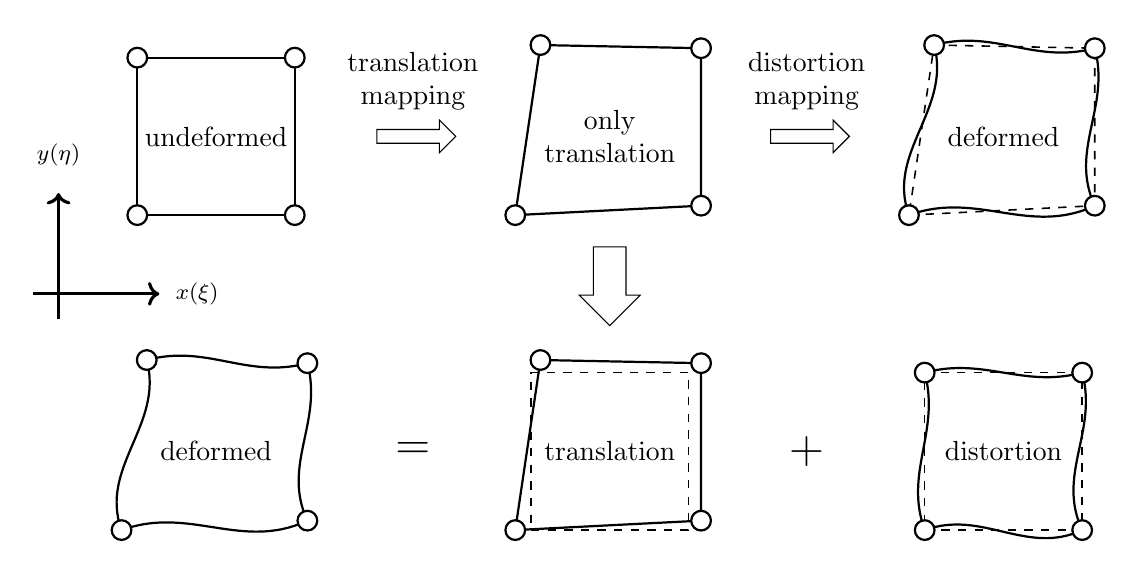
\begin{tikzpicture}[x=2mm,y=2mm]
\def\a{0+20}\def\b{180+25}\def\c{270+15}\def\d{360+15}
\CoorOrigin{-5,-5}[x(\xi)][y(\eta)]{8}
\node[single arrow,draw,minimum height=10mm,single arrow head extend=1.2mm,inner sep=.8mm]at(17.5,5){};
\node[single arrow,draw,minimum height=10mm,single arrow head extend=1.2mm,inner sep=.8mm]at(42.5,5){};
\node[align=center]at(17.5,8.5){translation\\mapping};
\node[align=center]at(42.5,8.5){distortion\\mapping};
\node[single arrow,draw,minimum height=10mm,single arrow head extend=1.8mm,inner sep=2mm,shape border rotate=270]at(30,-4){};
\node at(17.5,-15){\LARGE$=$};
\node at(42.5,-15){\LARGE$+$};
\node[align=center]at(5,5){undeformed};
\node[align=center]at(30,5){only\\translation};
\node[align=center]at(55,5){deformed};
\node[align=center]at(5,-15){deformed};
\node[align=center]at(30,-15){translation};
\node[align=center]at(55,-15){distortion};
\begin{scope}[xshift=00mm,every node/.style={circle,thick,draw,fill=white,inner sep=0,minimum size=2.5mm}]
\draw[thick]
(0,0)node{}--(10,0)node{}--(10,10)node{}--(0,10)node{}--cycle;
\end{scope}
\begin{scope}[xshift=50mm,every node/.style={circle,thick,draw,fill=white,inner sep=0,minimum size=2.5mm}]
\draw[thick]
(0-1,0)node{}--(10+.8,0+.6)node{}--(10+.8,10+.6)node{}--(0+.6,10+.8)node{}--cycle;
\end{scope}
\begin{scope}[xshift=100mm,every node/.style={circle,thick,draw,fill=white,inner sep=0,minimum size=2.5mm}]
\draw[dashed,line width=.2mm]
(0-1,0)--(10+.8,0+.6)--(10+.8,10+.6)--(0+.6,10+.8)--cycle;
\draw[thick]
(0-1,0)node{}to[out=\a,in=\b]
(10+.8,0+.6)node{}to[out=\b-90,in=\c]
(10+.8,10+.6)node{}to[out=\c-90,in=\d]
(0+.6,10+.8)node{}to[out=\d-90,in=\a+90]cycle;
\end{scope}
\begin{scope}[xshift=00mm,yshift=-40mm,every node/.style={circle,thick,draw,fill=white,inner sep=0,minimum size=2.5mm}]
\draw[thick]
(0-1,0)node{}to[out=\a,in=\b]
(10+.8,0+.6)node{}to[out=\b-90,in=\c]
(10+.8,10+.6)node{}to[out=\c-90,in=\d]
(0+.6,10+.8)node{}to[out=\d-90,in=\a+90]cycle;
\end{scope}
\begin{scope}[xshift=50mm,yshift=-40mm,every node/.style={circle,thick,draw,fill=white,inner sep=0,minimum size=2.5mm}]
\draw[dashed,line width=.2mm]
(0,0)--(10,0)--(10,10)--(0,10)--cycle;
\draw[thick]
(0-1,0)node{}--(10+.8,0+.6)node{}--(10+.8,10+.6)node{}--(0+.6,10+.8)node{}--cycle;
\end{scope}
\begin{scope}[xshift=100mm,yshift=-40mm,every node/.style={circle,thick,draw,fill=white,inner sep=0,minimum size=2.5mm}]
\draw[dashed,line width=.2mm]
(0,0)--(10,0)--(10,10)--(0,10)--cycle;
\draw[thick]
(0,0)node{}to[out=\a,in=\b]
(10,0)node{}to[out=\b-90,in=\c]
(10,10)node{}to[out=\c-90,in=\d]
(0,10)node{}to[out=\d-90,in=\a+90]cycle;
\end{scope}
\end{tikzpicture}
\caption{deformation decomposition}\label{fig:decompose_deformation}
\end{figure}
\subsection{Stress Patterns}
Due to its mixed nature, GCMQ interpolates stress field over element domain by using a complete quadratic polynomial derived from a quartic Airy stress function, the explicit expression of which can be written as
\begin{gather}
\mathbold{\sigma}=\begin{bmatrix}
	\sigma_x & \sigma_y & \tau_{xy}
\end{bmatrix}^\mT=\mathbold{\phi}_\sigma\mathbold{\alpha},
\end{gather}
with $\mathbold{\alpha}=\begin{bmatrix}
	\alpha_1 & \alpha_2 & \alpha_3 & \cdots & \alpha_{11}
\end{bmatrix}^\mT$ are interpolation parameters and
\begin{gather}\label{eq:stress_patterns}
\mathbold{\phi}_\sigma=
\left[\begin{array}{ccc|cc|cc|cc|cc}
	1 & 0 & 0 & 0 & y & 0  & x  &  0   & 2xy  &   -x^2   & 2y^2-x^2 \\
	0 & 1 & 0 & x & 0 & y  & 0  & 2xy  &  0   & 2x^2-y^2 &   -y^2   \\
	0 & 0 & 1 & 0 & 0 & -x & -y & -x^2 & -y^2 &   2xy    &   2xy
\end{array}\right],
\end{gather}
where $x$ and $y$ are global coordinates.

Some of the stress patterns that \eqsref{eq:stress_patterns} can represent are illustrated in \figref{fig:stress_patterns}. The corresponding Airy stress terms are also shown in the same figure. For conventional FEM analyses, external loads are typically applied as (or converted to) concentrated nodal forces. This leads to a lower order distribution of stress field within element domain. However, a constant or (incomplete) linear interpolation, as commonly adopted in existing classic elements, is not sufficient to properly describe stress distributions in certain loading cases. With a quadratic distribution, as can be seen in the figure, most stress patterns in loaded wall--like structures (without boundary tractions) can be covered.
\begin{figure}[H]
\centering\scriptsize
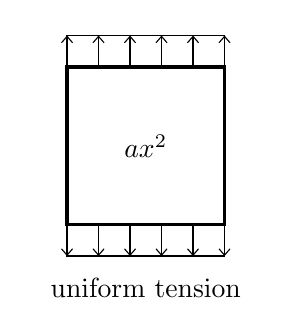
\begin{tikzpicture}[>={Straight Barb[width=4pt]}]
\clip(-.5,-1)rectangle(2.5,2.5);
\draw[line width=.4mm](0,0)rectangle(2,2);
\draw(0,0)rectangle(2,-.4);
\draw(0,2)rectangle(2,2.4);
\foreach\x in{0,.4,.8,1.2,1.6,2}{
\draw[->](\x,0)--++(0,-.4);
\draw[->](\x,2)--++(0,.4);
};
\node at(1,1){$ax^2$};
\node at(1,-.8){uniform tension};
\end{tikzpicture}
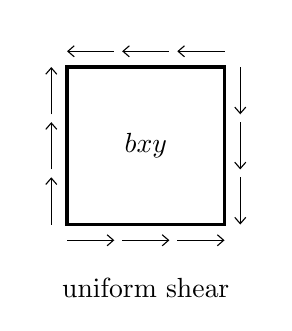
\begin{tikzpicture}[>={Straight Barb[width=4pt]}]
\clip(-.5,-1)rectangle(2.5,2.5);
\draw[line width=.4mm](0,0)rectangle(2,2);
\foreach\x in{0,.7,1.4}{
\draw[->](\x,-.2)--++(.6,0);
\draw[<-](2.2,\x)--++(0,.6);
\draw[<-](\x,2.2)--++(.6,0);
\draw[->](-.2,\x)--++(0,.6);
};
\node at(1,1){$bxy$};
\node at(1,-.8){uniform shear};
\end{tikzpicture}
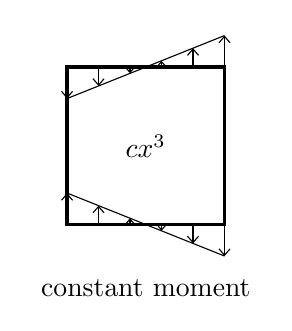
\begin{tikzpicture}[>={Straight Barb[width=4pt]}]
\clip(-.5,-1)rectangle(2.5,2.5);
\draw[line width=.4mm](0,0)rectangle(2,2);
\draw(0,.4)--(2,-.4);
\draw(0,1.6)--(2,2.4);
\foreach\x in{0,.4,.8,1.2,1.6,2}{
\draw[->](\x,0)--++(0,-.4*\x+.4);
\draw[->](\x,2)--++(0,.4*\x-.4);
};
\node at(1,1){$cx^3$};
\node at(1,-.8){constant moment};
\end{tikzpicture}
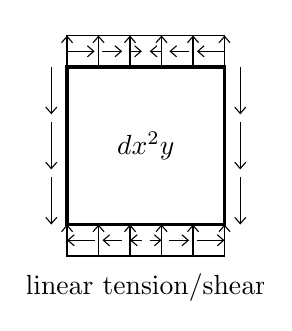
\begin{tikzpicture}[>={Straight Barb[width=4pt]}]
\clip(-.5,-1)rectangle(2.5,2.5);
\draw[line width=.4mm](0,0)rectangle(2,2);
\draw(0,0)rectangle(2,-.4);
\draw(0,2)rectangle(2,2.4);
\foreach\x in{0,.4,.8,1.2,1.6,2}{
\draw[<-](\x,0)--++(0,-.4);
\draw[->](\x,2)--++(0,.4);
}
\foreach\x in{0,.7,1.4}{
\draw[<-](2.2,\x)--++(0,.6);
\draw[<-](-.2,\x)--++(0,.6);
}
\draw[<-](0,-.2)--++(.35,0);
\draw[<-](.45,-.2)--++(.25,0);
\draw[<-](.8,-.2)--++(.15,0);
\draw[->](1.05,-.2)--++(.15,0);
\draw[->](1.3,-.2)--++(.25,0);
\draw[->](1.65,-.2)--++(.35,0);
\draw[->](0,2.2)--++(.35,0);
\draw[->](.45,2.2)--++(.25,0);
\draw[->](.8,2.2)--++(.15,0);
\draw[<-](1.05,2.2)--++(.15,0);
\draw[<-](1.3,2.2)--++(.25,0);
\draw[<-](1.65,2.2)--++(.35,0);
\node at(1,1){$dx^2y$};
\node at(1,-.8){linear tension/shear};
\end{tikzpicture}
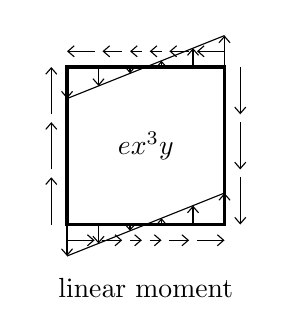
\begin{tikzpicture}[>={Straight Barb[width=4pt]}]
\clip(-.5,-1)rectangle(2.5,2.5);
\draw[line width=.4mm](0,0)rectangle(2,2);
\draw(0,-.4)--(2,.4);
\draw(0,1.6)--(2,2.4);
\foreach\x in{0,.4,.8,1.2,1.6,2}{
\draw[->](\x,0)--++(0,.4*\x-.4);
\draw[->](\x,2)--++(0,.4*\x-.4);
}
\foreach\x in{0,.7,1.4}{
\draw[<-](2.2,\x)--++(0,.6);
\draw[->](-.2,\x)--++(0,.6);
}
\draw[->](0,-.2)--++(.35,0);
\draw[->](.45,-.2)--++(.25,0);
\draw[->](.8,-.2)--++(.15,0);
\draw[->](1.05,-.2)--++(.15,0);
\draw[->](1.3,-.2)--++(.25,0);
\draw[->](1.65,-.2)--++(.35,0);
\draw[<-](0,2.2)--++(.35,0);
\draw[<-](.45,2.2)--++(.25,0);
\draw[<-](.8,2.2)--++(.15,0);
\draw[<-](1.05,2.2)--++(.15,0);
\draw[<-](1.3,2.2)--++(.25,0);
\draw[<-](1.65,2.2)--++(.35,0);
\node at(1,1){$ex^3y$};
\node at(1,-.8){linear moment};
\end{tikzpicture}
\caption{corresponding stress patterns of selected Airy stress function terms}\label{fig:stress_patterns}
\end{figure}
\subsection{Section Resultant Forces}
Engineers are more interested in section resultant forces as from which useful information can be extracted to guide structural design. By definition, section resultant forces, including moment $M$, axial force $F$ and shear force $V$, can be obtained by integrating stress field $\mathbold{\sigma}$ over the target section, which degenerates to a line in a 2D scenario.

For any section within element domain, three resultant forces could be expressed as
\begin{gather}\label{eq:resultant_force}
F=\int\sigma_w~\md{A},\quad{}V=\int\tau_s~\md{A},\quad{}M=\int{}s\cdot\sigma_w~\md{A},
\end{gather}
in which $s$ and $w$ are local coordinates of the target section/line, $\sigma_w$ and $\tau_s$ are normal and shear stresses acting along corresponding directions. The $w$ axis points to the outer normal direction while the $s$ axis coincides with the section inclination. Since a uniform thickness $t$ is assumed, $\md{A}$ simply equals $t\cdot\md{s}$. The direct computation of cross section resultant forces would be useful with very coarse mesh grids. However, as moments are taken about edge centres, it would be less meaningful to process moment outputs alone if multiple elements are defined along the target section.

Here only the edge 2 that connects nodes 2 and 3 is discussed for illustration. \figref{fig:reference_frame} shows the definitions of three different reference frames: the global coordinate system $x$-$y$, the parent coordinate system $\xi$-$\eta$ and the local coordinate system $s$-$w$ for edge 2. In this case, $s$ and $\eta$ are of the same direction so that
\begin{gather*}
\md{s}=\dfrac{e_2}{2}\md{\eta},
\end{gather*}
where $e_2$ is the length of edge 2. The stress $\mathbold{\sigma}$ can be transformed from $x$-$y$ system to $w$-$s$ system as follows,
\begin{gather}\label{eq:edge_stress}
\bar{\mathbold{\sigma}}_2\left(\eta\right)=\begin{bmatrix}
\sigma_w\\\tau_s
\end{bmatrix}=\mathbold{L}_2\mathbold{\sigma}_2=\mathbold{L}_2\mathbold{\phi}_\sigma\left(\xi,\eta\right)\Big|_{\xi=1}\mathbold{\alpha},
\end{gather}
with
\begin{gather}
\mathbold{L}_2=\begin{bmatrix}
l^2_2&m^2_2&2l_2m_2\\
-l_2m_2&l_2m_2&l^2_2-m^2_2
\end{bmatrix},
\end{gather}
where $l_2=\cos\theta_2$ and $m_2=\sin\theta_2$ are directional cosines with $\theta_2$ denotes the anticlockwise angle measured from $x$-axis to $w$-axis. The subscript $n=1,2,3,4$ denotes four edge labels. The transformation matrix $\mathbold{L}_n$ can be easily derived from the free body diagram of a wedge subjected to given stress $\mathbold{\sigma}$. It shall be emphasised that the original $\mathbold{\phi}_\sigma$ is a function of global coordinates $x$ and $y$. But in \eqsref{eq:edge_stress} it is expressed as a function of the parent coordinates $\xi$ and $\eta$. The transformation between parent and global coordinates is given by the Jacobian matrix that is available via isoparametric mapping.
\begin{figure}[htb]
\footnotesize\centering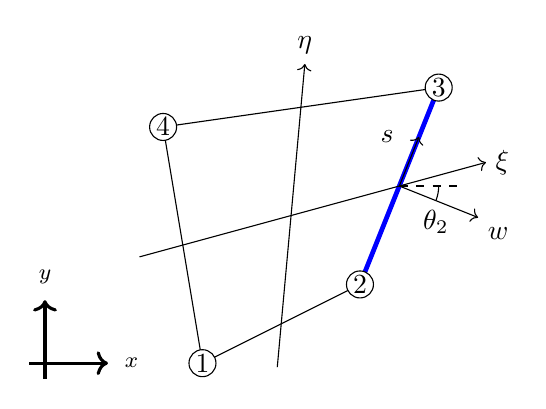
\begin{tikzpicture}
\CoorOrigin{-1,-1}
\coordinate(A)at(1,-1);
\coordinate(B)at(3,0);
\coordinate(C)at(4,2.5);
\coordinate(D)at(.5,2);
\coordinate(E)at($(A)!.5!(D)$);
\coordinate(F)at($(B)!.5!(C)$);
\coordinate(G)at($(A)!.5!(B)$);
\coordinate(H)at($(C)!.5!(D)$);
\draw[blue,line width=.6mm](B)--(C);
\draw(B)node[draw,circle,fill=white,inner sep=.2mm]{$2$}--(A)node[draw,circle,fill=white,inner sep=.2mm]{$1$}--(D)node[draw,circle,fill=white,inner sep=.2mm]{$4$}--(C)node[draw,circle,fill=white,inner sep=.2mm]{$3$};
\draw[->]($(E)!-.2!(F)$)--($(E)!1.4!(F)$)node[anchor=west]{$\xi$};
\draw[->]($(G)!-.2!(H)$)--($(G)!1.2!(H)$)node[fill=white,anchor=south]{$\eta$};
\draw[->](F)--($(F)!.5!(C)$)node[fill=white,left=2mm]{$s$};
\draw[->](F)--++(1,-.4)node[fill=white,anchor=north west]{$w$};
\draw($(F)+(.5,0)$)arc(0:-21.8:.5)node[anchor=north]{$\theta_2$};
\draw[dashed](F)--++(.8,0);
\end{tikzpicture}
\caption{definitions of reference frames}\label{fig:reference_frame}
\end{figure}

Then three section resultant forces can be simply integrated as
\begin{gather*}
F_2=\int\sigma_w~\md{A}=\dfrac{e_2t}{2}\int_{-1}^{1}\sigma_w~\md{\eta},\\
V_2=\int\tau_s~\md{A}=\dfrac{e_2t}{2}\int_{-1}^{1}\tau_s~\md{\eta},\\
M_2=\int{}s\cdot\sigma_w~\md{A}=\dfrac{e_2^2t}{4}\int_{-1}^{1}\eta\cdot\sigma_w~\md{\eta}.
\end{gather*}
Since $\mathbold{L}_n$ is a constant matrix for each boundary, they can be further expressed as
\begin{gather}
\begin{bmatrix}
F_2\\V_2
\end{bmatrix}=\dfrac{e_2t}{2}\mathbold{L}_2\mathbold{C}_2\mathbold{\alpha},\qquad
M_2=\dfrac{e_2^2t}{4}\mathbold{L}_2^{\left(1\right)}\mathbold{D}_2\mathbold{\alpha}.
\end{gather}
where
\begin{gather}
\mathbold{C}_2=\int_{-1}^{1}\mathbold{\phi}_\sigma\left(\xi,\eta\right)\Big|_{\xi=1}~\md{\eta},\qquad
\mathbold{D}_2=\int_{-1}^{1}\eta\cdot\mathbold{\phi}_\sigma\left(\xi,\eta\right)\Big|_{\xi=1}~\md{\eta}.
\end{gather}
The symbol $\mathbold{L}_2^{\left(1\right)}$ denotes the first row of $\mathbold{L}_2$. The matrices $\mathbold{C}_2$ and $\mathbold{D}_2$, that contain up to cubic terms, can be precisely evaluated by a two--point Gaussian scheme. For other edges, the transformation can be derived in a similar fashion. A closed form of above resultant forces is available only if the element is a parallelogram or rectangle.

The procedure described above is an alternative to simplify the recovery of stress field and resultant forces. Nevertheless, traditional post-processing procedures can also be applied. Resultant forces can also be obtained by integrating the material stress field, which can be obtained from material stresses at integration points via proper averaging methods. This is beyond the scope of this paper.
\section{Material Models}
\subsection{Concrete}
Two concrete material models, namely the fixed crack model (FCM) and the damage plasticity model (CDP), are employed in this work. FCM model allows flexible definitions of backbones and unloading/reloading responses. It is used in applications under cyclic loadings. However, FCM model does not support regularisation of size effect, hence it is not suitable for studies regarding mesh refinement. In contrast, CDP model is derived based on classic plasticity theory and supports regularisation, hence it can be used to study convergence of the proposed element. CDP model is only used in applications under monotonic loadings due to its limitations in calibration of unloading/reloading behaviour. Details of two models are briefly introduced.
\subsubsection{Fixed Crack Concrete Model}
A fixed crack planar concrete model (FCM) that incorporates a Rankine type square initial yield surface is used. The formulation resembles the one presented by \citet{Crisfield1989}. Similar formulations can be seen elsewhere. For simplicity, coupling effect between two crack directions is not considered. For each direction, the uniaxial response adopts Tsai's equation \citep{Tsai1988}. The normalised equation can be written as
\begin{gather*}
y=\dfrac{mx}{1+\left(m-\dfrac{n}{n-1}\right)x+\dfrac{x^n}{n-1}},
\end{gather*}
where $x$ and $y$ are normalised strain and stress, $m$ is a constant that controls the ratio of the initial modulus and the secant modulus at peak stress while $n$ is another constant that controls the shape of descending portion of the curve. By adjusting $m$ and $n$, both compression and tension backbones can be represented. A simple piece--wise linear unloading/reloading rule is applied. An illustrative example is depicted in \figref{fig:concrete}. It shall be noted that the material parameters are scaled for a clearer plot and may not represent a real concrete behaviour. The shear response is assumed to be bilinear elastic with a shear retention factor to account for dowel action, aggregate locking, etc. Such a concrete model is simple and in most cases convergence can be achieved with little computational effort.
\subsubsection{Concrete Damage Plasticity Model}
To refine analysis results, this paper also adopts another type of concrete constitutive models that is based on classic plasticity and damage theory, namely the concrete damage plasticity (CDP) model. The yield surface of which is defined in the principal stress space, the first stress invariant $I_1$ is included in its expression so confinement can be automatically accounted for. Details of the model can be found elsewhere \citep{Lee1998}. Based on the additive decomposition of strain, the stress $\sigma$ can be expressed as
\begin{gather*}
\sigma=\left(1-d\right)E\left(\varepsilon-\varepsilon_p\right),
\end{gather*}
in which $E$ the elastic stiffness, $\varepsilon$ is the total strain, $\varepsilon_p$ is the plastic strain and $d=f(d_t,d_c)$ is the damage/degradation factor defined as a function of tensile and compressive damage indices $d_t$ and $d_c$, the evolution of which depends on two material constants $g_t$ and $g_c$. By adjusting these two parameters, the CDP model is able to regularise material response to obtain mesh independent results. The normalised fracture energy $g_t$ is defined as fracture energy per unit length, viz., $g_t=G_F/l_c$ where $G_F$ is the first mode fracture energy and $l_c$ is the characteristic length. Although there is no correspondence in compression, for numerical convenience, the conjugate part of $g_t$, namely $g_c$, is defined in the model. Alternatively, they can be interpreted as the total areas under stress envelops expressed in terms of $\varepsilon_p$ \citep{Lubliner1989}.

The damage indices $d_t$ and $d_c$ ranging from zero to unity can be used to indicate the degree of stiffness degradation. Since cracking is modelled in a smeared approach, $d_t$ and $d_c$ may not necessarily be directly related to concrete crack and crush. Meanwhile, since coarse meshes are used in the following numerical examples, only an averaged effect can be represented. For the same reason, confinement is not considered separately in this work.
\subsection{Reinforcement}
In this work, reinforcement is assumed to be uniformly distributed and implemented in a smeared approach. As a result, the real rebar layouts are not explicitly modelled. An alternative could be the combination of both concentrated and smeared reinforcements. The uniaxial Menegotto--Pinto steel model \citep{Menegotto1973} is used to simulate the behaviour of reinforcement along two orthogonal directions. A representative example of the model is shown in \figref{fig:steel}.
\begin{figure}[htb]
\centering\scriptsize
\begin{subfigure}[b]{.48\textwidth}\centering
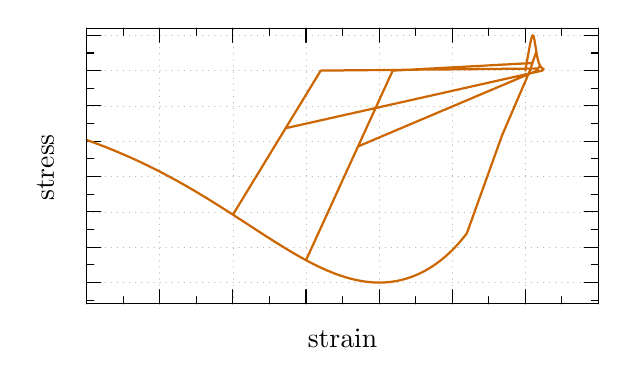
\begin{tikzpicture}[gnuplot]
%% generated with GNUPLOT 5.2p6 (Lua 5.3; terminal rev. Nov 2018, script rev. 107)
%% 03/05/2019 03:30:03
\path (0.000,0.000) rectangle (6.500,3.500);
\gpcolor{color=gp lt color border}
\gpsetlinetype{gp lt border}
\gpsetdashtype{gp dt solid}
\gpsetlinewidth{1.00}
\draw[gp path] (0.000,0.045)--(0.090,0.045);
\draw[gp path] (6.499,0.045)--(6.409,0.045);
\gpcolor{color=gp lt color axes}
\gpsetlinetype{gp lt axes}
\gpsetdashtype{gp dt axes}
\gpsetlinewidth{0.50}
\draw[gp path] (0.000,0.269)--(6.499,0.269);
\gpcolor{color=gp lt color border}
\gpsetlinetype{gp lt border}
\gpsetdashtype{gp dt solid}
\gpsetlinewidth{1.00}
\draw[gp path] (0.000,0.269)--(0.180,0.269);
\draw[gp path] (6.499,0.269)--(6.319,0.269);
\draw[gp path] (0.000,0.493)--(0.090,0.493);
\draw[gp path] (6.499,0.493)--(6.409,0.493);
\gpcolor{color=gp lt color axes}
\gpsetlinetype{gp lt axes}
\gpsetdashtype{gp dt axes}
\gpsetlinewidth{0.50}
\draw[gp path] (0.000,0.718)--(6.499,0.718);
\gpcolor{color=gp lt color border}
\gpsetlinetype{gp lt border}
\gpsetdashtype{gp dt solid}
\gpsetlinewidth{1.00}
\draw[gp path] (0.000,0.718)--(0.180,0.718);
\draw[gp path] (6.499,0.718)--(6.319,0.718);
\draw[gp path] (0.000,0.942)--(0.090,0.942);
\draw[gp path] (6.499,0.942)--(6.409,0.942);
\gpcolor{color=gp lt color axes}
\gpsetlinetype{gp lt axes}
\gpsetdashtype{gp dt axes}
\gpsetlinewidth{0.50}
\draw[gp path] (0.000,1.166)--(6.499,1.166);
\gpcolor{color=gp lt color border}
\gpsetlinetype{gp lt border}
\gpsetdashtype{gp dt solid}
\gpsetlinewidth{1.00}
\draw[gp path] (0.000,1.166)--(0.180,1.166);
\draw[gp path] (6.499,1.166)--(6.319,1.166);
\draw[gp path] (0.000,1.391)--(0.090,1.391);
\draw[gp path] (6.499,1.391)--(6.409,1.391);
\gpcolor{color=gp lt color axes}
\gpsetlinetype{gp lt axes}
\gpsetdashtype{gp dt axes}
\gpsetlinewidth{0.50}
\draw[gp path] (0.000,1.615)--(6.499,1.615);
\gpcolor{color=gp lt color border}
\gpsetlinetype{gp lt border}
\gpsetdashtype{gp dt solid}
\gpsetlinewidth{1.00}
\draw[gp path] (0.000,1.615)--(0.180,1.615);
\draw[gp path] (6.499,1.615)--(6.319,1.615);
\draw[gp path] (0.000,1.839)--(0.090,1.839);
\draw[gp path] (6.499,1.839)--(6.409,1.839);
\gpcolor{color=gp lt color axes}
\gpsetlinetype{gp lt axes}
\gpsetdashtype{gp dt axes}
\gpsetlinewidth{0.50}
\draw[gp path] (0.000,2.064)--(6.499,2.064);
\gpcolor{color=gp lt color border}
\gpsetlinetype{gp lt border}
\gpsetdashtype{gp dt solid}
\gpsetlinewidth{1.00}
\draw[gp path] (0.000,2.064)--(0.180,2.064);
\draw[gp path] (6.499,2.064)--(6.319,2.064);
\draw[gp path] (0.000,2.288)--(0.090,2.288);
\draw[gp path] (6.499,2.288)--(6.409,2.288);
\gpcolor{color=gp lt color axes}
\gpsetlinetype{gp lt axes}
\gpsetdashtype{gp dt axes}
\gpsetlinewidth{0.50}
\draw[gp path] (0.000,2.512)--(6.499,2.512);
\gpcolor{color=gp lt color border}
\gpsetlinetype{gp lt border}
\gpsetdashtype{gp dt solid}
\gpsetlinewidth{1.00}
\draw[gp path] (0.000,2.512)--(0.180,2.512);
\draw[gp path] (6.499,2.512)--(6.319,2.512);
\draw[gp path] (0.000,2.736)--(0.090,2.736);
\draw[gp path] (6.499,2.736)--(6.409,2.736);
\gpcolor{color=gp lt color axes}
\gpsetlinetype{gp lt axes}
\gpsetdashtype{gp dt axes}
\gpsetlinewidth{0.50}
\draw[gp path] (0.000,2.961)--(6.499,2.961);
\gpcolor{color=gp lt color border}
\gpsetlinetype{gp lt border}
\gpsetdashtype{gp dt solid}
\gpsetlinewidth{1.00}
\draw[gp path] (0.000,2.961)--(0.180,2.961);
\draw[gp path] (6.499,2.961)--(6.319,2.961);
\draw[gp path] (0.000,3.185)--(0.090,3.185);
\draw[gp path] (6.499,3.185)--(6.409,3.185);
\gpcolor{color=gp lt color axes}
\gpsetlinetype{gp lt axes}
\gpsetdashtype{gp dt axes}
\gpsetlinewidth{0.50}
\draw[gp path] (0.000,3.409)--(6.499,3.409);
\gpcolor{color=gp lt color border}
\gpsetlinetype{gp lt border}
\gpsetdashtype{gp dt solid}
\gpsetlinewidth{1.00}
\draw[gp path] (0.000,3.409)--(0.180,3.409);
\draw[gp path] (6.499,3.409)--(6.319,3.409);
\gpcolor{color=gp lt color axes}
\gpsetlinetype{gp lt axes}
\gpsetdashtype{gp dt axes}
\gpsetlinewidth{0.50}
\draw[gp path] (0.000,0.000)--(0.000,3.499);
\gpcolor{color=gp lt color border}
\gpsetlinetype{gp lt border}
\gpsetdashtype{gp dt solid}
\gpsetlinewidth{1.00}
\draw[gp path] (0.000,0.000)--(0.000,0.180);
\draw[gp path] (0.000,3.499)--(0.000,3.319);
\draw[gp path] (0.464,0.000)--(0.464,0.090);
\draw[gp path] (0.464,3.499)--(0.464,3.409);
\gpcolor{color=gp lt color axes}
\gpsetlinetype{gp lt axes}
\gpsetdashtype{gp dt axes}
\gpsetlinewidth{0.50}
\draw[gp path] (0.928,0.000)--(0.928,3.499);
\gpcolor{color=gp lt color border}
\gpsetlinetype{gp lt border}
\gpsetdashtype{gp dt solid}
\gpsetlinewidth{1.00}
\draw[gp path] (0.928,0.000)--(0.928,0.180);
\draw[gp path] (0.928,3.499)--(0.928,3.319);
\draw[gp path] (1.393,0.000)--(1.393,0.090);
\draw[gp path] (1.393,3.499)--(1.393,3.409);
\gpcolor{color=gp lt color axes}
\gpsetlinetype{gp lt axes}
\gpsetdashtype{gp dt axes}
\gpsetlinewidth{0.50}
\draw[gp path] (1.857,0.000)--(1.857,3.499);
\gpcolor{color=gp lt color border}
\gpsetlinetype{gp lt border}
\gpsetdashtype{gp dt solid}
\gpsetlinewidth{1.00}
\draw[gp path] (1.857,0.000)--(1.857,0.180);
\draw[gp path] (1.857,3.499)--(1.857,3.319);
\draw[gp path] (2.321,0.000)--(2.321,0.090);
\draw[gp path] (2.321,3.499)--(2.321,3.409);
\gpcolor{color=gp lt color axes}
\gpsetlinetype{gp lt axes}
\gpsetdashtype{gp dt axes}
\gpsetlinewidth{0.50}
\draw[gp path] (2.785,0.000)--(2.785,3.499);
\gpcolor{color=gp lt color border}
\gpsetlinetype{gp lt border}
\gpsetdashtype{gp dt solid}
\gpsetlinewidth{1.00}
\draw[gp path] (2.785,0.000)--(2.785,0.180);
\draw[gp path] (2.785,3.499)--(2.785,3.319);
\draw[gp path] (3.250,0.000)--(3.250,0.090);
\draw[gp path] (3.250,3.499)--(3.250,3.409);
\gpcolor{color=gp lt color axes}
\gpsetlinetype{gp lt axes}
\gpsetdashtype{gp dt axes}
\gpsetlinewidth{0.50}
\draw[gp path] (3.714,0.000)--(3.714,3.499);
\gpcolor{color=gp lt color border}
\gpsetlinetype{gp lt border}
\gpsetdashtype{gp dt solid}
\gpsetlinewidth{1.00}
\draw[gp path] (3.714,0.000)--(3.714,0.180);
\draw[gp path] (3.714,3.499)--(3.714,3.319);
\draw[gp path] (4.178,0.000)--(4.178,0.090);
\draw[gp path] (4.178,3.499)--(4.178,3.409);
\gpcolor{color=gp lt color axes}
\gpsetlinetype{gp lt axes}
\gpsetdashtype{gp dt axes}
\gpsetlinewidth{0.50}
\draw[gp path] (4.642,0.000)--(4.642,3.499);
\gpcolor{color=gp lt color border}
\gpsetlinetype{gp lt border}
\gpsetdashtype{gp dt solid}
\gpsetlinewidth{1.00}
\draw[gp path] (4.642,0.000)--(4.642,0.180);
\draw[gp path] (4.642,3.499)--(4.642,3.319);
\draw[gp path] (5.106,0.000)--(5.106,0.090);
\draw[gp path] (5.106,3.499)--(5.106,3.409);
\gpcolor{color=gp lt color axes}
\gpsetlinetype{gp lt axes}
\gpsetdashtype{gp dt axes}
\gpsetlinewidth{0.50}
\draw[gp path] (5.571,0.000)--(5.571,3.499);
\gpcolor{color=gp lt color border}
\gpsetlinetype{gp lt border}
\gpsetdashtype{gp dt solid}
\gpsetlinewidth{1.00}
\draw[gp path] (5.571,0.000)--(5.571,0.180);
\draw[gp path] (5.571,3.499)--(5.571,3.319);
\draw[gp path] (6.035,0.000)--(6.035,0.090);
\draw[gp path] (6.035,3.499)--(6.035,3.409);
\gpcolor{color=gp lt color axes}
\gpsetlinetype{gp lt axes}
\gpsetdashtype{gp dt axes}
\gpsetlinewidth{0.50}
\draw[gp path] (6.499,0.000)--(6.499,3.499);
\gpcolor{color=gp lt color border}
\gpsetlinetype{gp lt border}
\gpsetdashtype{gp dt solid}
\gpsetlinewidth{1.00}
\draw[gp path] (6.499,0.000)--(6.499,0.180);
\draw[gp path] (6.499,3.499)--(6.499,3.319);
\draw[gp path] (0.000,3.499)--(0.000,0.000)--(6.499,0.000)--(6.499,3.499)--cycle;
\node[gp node center,rotate=-270] at (-0.492,1.749) {stress};
\node[gp node center] at (3.249,-0.461) {strain};
\gpcolor{rgb color={0.800,0.400,0.000}}
\gpsetlinewidth{2.00}
\draw[gp path] (5.571,2.961)--(5.580,3.013)--(5.589,3.066)--(5.598,3.118)--(5.608,3.170)%
  --(5.617,3.221)--(5.626,3.271)--(5.636,3.319)--(5.645,3.361)--(5.654,3.393)--(5.663,3.409)%
  --(5.673,3.402)--(5.682,3.371)--(5.691,3.321)--(5.701,3.261)--(5.710,3.202)--(5.701,3.174)%
  --(5.691,3.147)--(5.682,3.119)--(5.673,3.092)--(5.663,3.064)--(5.654,3.037)--(5.645,3.009)%
  --(5.636,2.981)--(5.626,2.955)--(5.617,2.934)--(5.608,2.912)--(5.598,2.891)--(5.589,2.869)%
  --(5.580,2.847)--(5.571,2.826)--(5.561,2.804)--(5.552,2.783)--(5.543,2.761)--(5.533,2.739)%
  --(5.524,2.718)--(5.515,2.696)--(5.506,2.674)--(5.496,2.653)--(5.487,2.631)--(5.478,2.610)%
  --(5.468,2.588)--(5.459,2.566)--(5.450,2.545)--(5.441,2.523)--(5.431,2.502)--(5.422,2.480)%
  --(5.413,2.458)--(5.403,2.437)--(5.394,2.415)--(5.385,2.394)--(5.376,2.372)--(5.366,2.350)%
  --(5.357,2.329)--(5.348,2.307)--(5.338,2.286)--(5.329,2.264)--(5.320,2.242)--(5.311,2.221)%
  --(5.301,2.199)--(5.292,2.177)--(5.283,2.156)--(5.273,2.134)--(5.264,2.108)--(5.255,2.082)%
  --(5.246,2.057)--(5.236,2.031)--(5.227,2.005)--(5.218,1.979)--(5.208,1.953)--(5.199,1.927)%
  --(5.190,1.902)--(5.181,1.876)--(5.171,1.850)--(5.162,1.824)--(5.153,1.798)--(5.143,1.772)%
  --(5.134,1.747)--(5.125,1.721)--(5.116,1.695)--(5.106,1.669)--(5.097,1.643)--(5.088,1.617)%
  --(5.079,1.592)--(5.069,1.566)--(5.060,1.540)--(5.051,1.514)--(5.041,1.488)--(5.032,1.463)%
  --(5.023,1.437)--(5.014,1.411)--(5.004,1.385)--(4.995,1.359)--(4.986,1.333)--(4.976,1.308)%
  --(4.967,1.282)--(4.958,1.256)--(4.949,1.230)--(4.939,1.204)--(4.930,1.178)--(4.921,1.153)%
  --(4.911,1.127)--(4.902,1.101)--(4.893,1.075)--(4.884,1.049)--(4.874,1.023)--(4.865,0.998)%
  --(4.856,0.972)--(4.846,0.946)--(4.837,0.920)--(4.828,0.895)--(4.819,0.883)--(4.809,0.871)%
  --(4.800,0.859)--(4.791,0.847)--(4.781,0.836)--(4.772,0.825)--(4.763,0.813)--(4.754,0.802)%
  --(4.744,0.791)--(4.735,0.781)--(4.726,0.770)--(4.716,0.759)--(4.707,0.749)--(4.698,0.739)%
  --(4.689,0.729)--(4.679,0.719)--(4.670,0.709)--(4.661,0.700)--(4.651,0.690)--(4.642,0.681)%
  --(4.633,0.672)--(4.624,0.663)--(4.614,0.654)--(4.605,0.645)--(4.596,0.636)--(4.586,0.628)%
  --(4.577,0.620)--(4.568,0.611)--(4.559,0.603)--(4.549,0.595)--(4.540,0.587)--(4.531,0.579)%
  --(4.521,0.572)--(4.512,0.564)--(4.503,0.557)--(4.494,0.549)--(4.484,0.542)--(4.475,0.535)%
  --(4.466,0.528)--(4.456,0.521)--(4.447,0.514)--(4.438,0.508)--(4.429,0.501)--(4.419,0.495)%
  --(4.410,0.488)--(4.401,0.482)--(4.391,0.476)--(4.382,0.470)--(4.373,0.464)--(4.364,0.458)%
  --(4.354,0.452)--(4.345,0.447)--(4.336,0.441)--(4.326,0.436)--(4.317,0.431)--(4.308,0.425)%
  --(4.299,0.420)--(4.289,0.415)--(4.280,0.410)--(4.271,0.405)--(4.261,0.401)--(4.252,0.396)%
  --(4.243,0.391)--(4.234,0.387)--(4.224,0.383)--(4.215,0.378)--(4.206,0.374)--(4.196,0.370)%
  --(4.187,0.366)--(4.178,0.362)--(4.169,0.358)--(4.159,0.354)--(4.150,0.351)--(4.141,0.347)%
  --(4.132,0.344)--(4.122,0.340)--(4.113,0.337)--(4.104,0.334)--(4.094,0.331)--(4.085,0.327)%
  --(4.076,0.324)--(4.067,0.322)--(4.057,0.319)--(4.048,0.316)--(4.039,0.313)--(4.029,0.311)%
  --(4.020,0.308)--(4.011,0.306)--(4.002,0.304)--(3.992,0.301)--(3.983,0.299)--(3.974,0.297)%
  --(3.964,0.295)--(3.955,0.293)--(3.946,0.291)--(3.937,0.289)--(3.927,0.288)--(3.918,0.286)%
  --(3.909,0.285)--(3.899,0.283)--(3.890,0.282)--(3.881,0.280)--(3.872,0.279)--(3.862,0.278)%
  --(3.853,0.277)--(3.844,0.276)--(3.834,0.275)--(3.825,0.274)--(3.816,0.273)--(3.807,0.273)%
  --(3.797,0.272)--(3.788,0.271)--(3.779,0.271)--(3.769,0.270)--(3.760,0.270)--(3.751,0.270)%
  --(3.742,0.269)--(3.732,0.269)--(3.723,0.269)--(3.714,0.269)--(3.704,0.269)--(3.695,0.269)%
  --(3.686,0.270)--(3.677,0.270)--(3.667,0.270)--(3.658,0.270)--(3.649,0.271)--(3.639,0.271)%
  --(3.630,0.272)--(3.621,0.273)--(3.612,0.273)--(3.602,0.274)--(3.593,0.275)--(3.584,0.276)%
  --(3.574,0.277)--(3.565,0.278)--(3.556,0.279)--(3.547,0.280)--(3.537,0.281)--(3.528,0.283)%
  --(3.519,0.284)--(3.509,0.286)--(3.500,0.287)--(3.491,0.289)--(3.482,0.290)--(3.472,0.292)%
  --(3.463,0.294)--(3.454,0.295)--(3.444,0.297)--(3.435,0.299)--(3.426,0.301)--(3.417,0.303)%
  --(3.407,0.305)--(3.398,0.307)--(3.389,0.309)--(3.379,0.312)--(3.370,0.314)--(3.361,0.316)%
  --(3.352,0.319)--(3.342,0.321)--(3.333,0.324)--(3.324,0.326)--(3.314,0.329)--(3.305,0.332)%
  --(3.296,0.334)--(3.287,0.337)--(3.277,0.340)--(3.268,0.343)--(3.259,0.346)--(3.249,0.349)%
  --(3.240,0.352)--(3.231,0.355)--(3.222,0.358)--(3.212,0.361)--(3.203,0.364)--(3.194,0.368)%
  --(3.185,0.371)--(3.175,0.374)--(3.166,0.378)--(3.157,0.381)--(3.147,0.385)--(3.138,0.388)%
  --(3.129,0.392)--(3.120,0.396)--(3.110,0.399)--(3.101,0.403)--(3.092,0.407)--(3.082,0.411)%
  --(3.073,0.414)--(3.064,0.418)--(3.055,0.422)--(3.045,0.426)--(3.036,0.430)--(3.027,0.434)%
  --(3.017,0.439)--(3.008,0.443)--(2.999,0.447)--(2.990,0.451)--(2.980,0.455)--(2.971,0.460)%
  --(2.962,0.464)--(2.952,0.468)--(2.943,0.473)--(2.934,0.477)--(2.925,0.482)--(2.915,0.486)%
  --(2.906,0.491)--(2.897,0.496)--(2.887,0.500)--(2.878,0.505)--(2.869,0.510)--(2.860,0.514)%
  --(2.850,0.519)--(2.841,0.524)--(2.832,0.529)--(2.822,0.534)--(2.813,0.538)--(2.804,0.543)%
  --(2.795,0.548)--(2.785,0.553)--(2.795,0.574)--(2.804,0.594)--(2.813,0.614)--(2.822,0.635)%
  --(2.832,0.655)--(2.841,0.675)--(2.850,0.695)--(2.860,0.716)--(2.869,0.736)--(2.878,0.756)%
  --(2.887,0.777)--(2.897,0.797)--(2.906,0.817)--(2.915,0.838)--(2.925,0.858)--(2.934,0.878)%
  --(2.943,0.898)--(2.952,0.919)--(2.962,0.939)--(2.971,0.959)--(2.980,0.980)--(2.990,1.000)%
  --(2.999,1.020)--(3.008,1.041)--(3.017,1.061)--(3.027,1.081)--(3.036,1.102)--(3.045,1.122)%
  --(3.055,1.142)--(3.064,1.162)--(3.073,1.183)--(3.082,1.203)--(3.092,1.223)--(3.101,1.244)%
  --(3.110,1.264)--(3.120,1.284)--(3.129,1.305)--(3.138,1.325)--(3.147,1.345)--(3.157,1.366)%
  --(3.166,1.386)--(3.175,1.406)--(3.185,1.426)--(3.194,1.447)--(3.203,1.467)--(3.212,1.487)%
  --(3.222,1.508)--(3.231,1.528)--(3.240,1.548)--(3.249,1.569)--(3.259,1.589)--(3.268,1.609)%
  --(3.277,1.630)--(3.287,1.650)--(3.296,1.670)--(3.305,1.690)--(3.314,1.711)--(3.324,1.731)%
  --(3.333,1.751)--(3.342,1.772)--(3.352,1.792)--(3.361,1.812)--(3.370,1.833)--(3.379,1.853)%
  --(3.389,1.873)--(3.398,1.893)--(3.407,1.914)--(3.417,1.934)--(3.426,1.954)--(3.435,1.975)%
  --(3.444,1.995)--(3.454,2.015)--(3.463,2.036)--(3.472,2.056)--(3.482,2.076)--(3.491,2.097)%
  --(3.500,2.117)--(3.509,2.137)--(3.519,2.157)--(3.528,2.178)--(3.537,2.198)--(3.547,2.218)%
  --(3.556,2.239)--(3.565,2.259)--(3.574,2.279)--(3.584,2.300)--(3.593,2.320)--(3.602,2.340)%
  --(3.612,2.361)--(3.621,2.381)--(3.630,2.401)--(3.639,2.421)--(3.649,2.442)--(3.658,2.462)%
  --(3.667,2.482)--(3.677,2.503)--(3.686,2.523)--(3.695,2.543)--(3.704,2.564)--(3.714,2.584)%
  --(3.723,2.604)--(3.732,2.625)--(3.742,2.645)--(3.751,2.665)--(3.760,2.685)--(3.769,2.706)%
  --(3.779,2.726)--(3.788,2.746)--(3.797,2.767)--(3.807,2.787)--(3.816,2.807)--(3.825,2.828)%
  --(3.834,2.848)--(3.844,2.868)--(3.853,2.888)--(3.862,2.909)--(3.872,2.929)--(3.881,2.949)%
  --(3.890,2.961)--(3.899,2.961)--(3.909,2.962)--(3.918,2.962)--(3.927,2.963)--(3.937,2.963)%
  --(3.946,2.964)--(3.955,2.964)--(3.964,2.965)--(3.974,2.965)--(3.983,2.966)--(3.992,2.966)%
  --(4.002,2.967)--(4.011,2.967)--(4.020,2.968)--(4.029,2.968)--(4.039,2.969)--(4.048,2.969)%
  --(4.057,2.970)--(4.067,2.971)--(4.076,2.971)--(4.085,2.972)--(4.094,2.972)--(4.104,2.973)%
  --(4.113,2.973)--(4.122,2.974)--(4.132,2.974)--(4.141,2.975)--(4.150,2.975)--(4.159,2.976)%
  --(4.169,2.976)--(4.178,2.977)--(4.187,2.977)--(4.196,2.978)--(4.206,2.978)--(4.215,2.979)%
  --(4.224,2.979)--(4.234,2.980)--(4.243,2.980)--(4.252,2.981)--(4.261,2.981)--(4.271,2.982)%
  --(4.280,2.982)--(4.289,2.983)--(4.299,2.983)--(4.308,2.984)--(4.317,2.984)--(4.326,2.985)%
  --(4.336,2.985)--(4.345,2.986)--(4.354,2.986)--(4.364,2.987)--(4.373,2.987)--(4.382,2.988)%
  --(4.391,2.988)--(4.401,2.989)--(4.410,2.989)--(4.419,2.990)--(4.429,2.990)--(4.438,2.991)%
  --(4.447,2.991)--(4.456,2.992)--(4.466,2.992)--(4.475,2.993)--(4.484,2.993)--(4.494,2.994)%
  --(4.503,2.994)--(4.512,2.995)--(4.521,2.995)--(4.531,2.996)--(4.540,2.996)--(4.549,2.997)%
  --(4.559,2.997)--(4.568,2.998)--(4.577,2.998)--(4.586,2.999)--(4.596,2.999)--(4.605,3.000)%
  --(4.614,3.000)--(4.624,3.001)--(4.633,3.001)--(4.642,3.002)--(4.651,3.002)--(4.661,3.003)%
  --(4.670,3.003)--(4.679,3.004)--(4.689,3.004)--(4.698,3.005)--(4.707,3.005)--(4.716,3.006)%
  --(4.726,3.006)--(4.735,3.007)--(4.744,3.007)--(4.754,3.008)--(4.763,3.008)--(4.772,3.009)%
  --(4.781,3.009)--(4.791,3.010)--(4.800,3.010)--(4.809,3.011)--(4.819,3.011)--(4.828,3.012)%
  --(4.837,3.012)--(4.846,3.013)--(4.856,3.013)--(4.865,3.014)--(4.874,3.014)--(4.884,3.015)%
  --(4.893,3.015)--(4.902,3.016)--(4.911,3.016)--(4.921,3.017)--(4.930,3.017)--(4.939,3.018)%
  --(4.949,3.018)--(4.958,3.019)--(4.967,3.019)--(4.976,3.020)--(4.986,3.020)--(4.995,3.021)%
  --(5.004,3.021)--(5.014,3.022)--(5.023,3.022)--(5.032,3.023)--(5.041,3.023)--(5.051,3.024)%
  --(5.060,3.024)--(5.069,3.025)--(5.079,3.025)--(5.088,3.026)--(5.097,3.027)--(5.106,3.027)%
  --(5.116,3.028)--(5.125,3.028)--(5.134,3.029)--(5.143,3.029)--(5.153,3.030)--(5.162,3.030)%
  --(5.171,3.031)--(5.181,3.031)--(5.190,3.032)--(5.199,3.032)--(5.208,3.033)--(5.218,3.033)%
  --(5.227,3.034)--(5.236,3.034)--(5.246,3.035)--(5.255,3.035)--(5.264,3.036)--(5.273,3.036)%
  --(5.283,3.037)--(5.292,3.037)--(5.301,3.038)--(5.311,3.038)--(5.320,3.039)--(5.329,3.039)%
  --(5.338,3.040)--(5.348,3.040)--(5.357,3.041)--(5.366,3.041)--(5.376,3.042)--(5.385,3.042)%
  --(5.394,3.043)--(5.403,3.043)--(5.413,3.044)--(5.422,3.044)--(5.431,3.045)--(5.441,3.045)%
  --(5.450,3.046)--(5.459,3.046)--(5.468,3.047)--(5.478,3.047)--(5.487,3.048)--(5.496,3.048)%
  --(5.506,3.049)--(5.515,3.049)--(5.524,3.050)--(5.533,3.050)--(5.543,3.051)--(5.552,3.051)%
  --(5.561,3.052)--(5.571,3.052)--(5.580,3.053)--(5.589,3.053)--(5.598,3.054)--(5.608,3.054)%
  --(5.617,3.055)--(5.626,3.055)--(5.636,3.056)--(5.645,3.056)--(5.654,3.057)--(5.663,3.064)%
  --(5.673,3.092)--(5.682,3.119)--(5.691,3.147)--(5.701,3.174)--(5.710,3.202)--(5.719,3.149)%
  --(5.728,3.106)--(5.738,3.072)--(5.747,3.046)--(5.756,3.026)--(5.747,3.011)--(5.738,2.995)%
  --(5.728,2.979)--(5.719,2.963)--(5.710,2.957)--(5.701,2.953)--(5.691,2.949)--(5.682,2.945)%
  --(5.673,2.942)--(5.663,2.938)--(5.654,2.934)--(5.645,2.930)--(5.636,2.926)--(5.626,2.922)%
  --(5.617,2.918)--(5.608,2.914)--(5.598,2.910)--(5.589,2.906)--(5.580,2.902)--(5.571,2.898)%
  --(5.561,2.894)--(5.552,2.890)--(5.543,2.886)--(5.533,2.883)--(5.524,2.879)--(5.515,2.875)%
  --(5.506,2.871)--(5.496,2.867)--(5.487,2.863)--(5.478,2.859)--(5.468,2.855)--(5.459,2.851)%
  --(5.450,2.847)--(5.441,2.843)--(5.431,2.839)--(5.422,2.835)--(5.413,2.831)--(5.403,2.827)%
  --(5.394,2.824)--(5.385,2.820)--(5.376,2.816)--(5.366,2.812)--(5.357,2.808)--(5.348,2.804)%
  --(5.338,2.800)--(5.329,2.796)--(5.320,2.792)--(5.311,2.788)--(5.301,2.784)--(5.292,2.780)%
  --(5.283,2.776)--(5.273,2.772)--(5.264,2.768)--(5.255,2.764)--(5.246,2.761)--(5.236,2.757)%
  --(5.227,2.753)--(5.218,2.749)--(5.208,2.745)--(5.199,2.741)--(5.190,2.737)--(5.181,2.733)%
  --(5.171,2.729)--(5.162,2.725)--(5.153,2.721)--(5.143,2.717)--(5.134,2.713)--(5.125,2.709)%
  --(5.116,2.705)--(5.106,2.702)--(5.097,2.698)--(5.088,2.694)--(5.079,2.690)--(5.069,2.686)%
  --(5.060,2.682)--(5.051,2.678)--(5.041,2.674)--(5.032,2.670)--(5.023,2.666)--(5.014,2.662)%
  --(5.004,2.658)--(4.995,2.654)--(4.986,2.650)--(4.976,2.646)--(4.967,2.643)--(4.958,2.639)%
  --(4.949,2.635)--(4.939,2.631)--(4.930,2.627)--(4.921,2.623)--(4.911,2.619)--(4.902,2.615)%
  --(4.893,2.611)--(4.884,2.607)--(4.874,2.603)--(4.865,2.599)--(4.856,2.595)--(4.846,2.591)%
  --(4.837,2.587)--(4.828,2.583)--(4.819,2.580)--(4.809,2.576)--(4.800,2.572)--(4.791,2.568)%
  --(4.781,2.564)--(4.772,2.560)--(4.763,2.556)--(4.754,2.552)--(4.744,2.548)--(4.735,2.544)%
  --(4.726,2.540)--(4.716,2.536)--(4.707,2.532)--(4.698,2.528)--(4.689,2.524)--(4.679,2.521)%
  --(4.670,2.517)--(4.661,2.513)--(4.651,2.509)--(4.642,2.505)--(4.633,2.501)--(4.624,2.497)%
  --(4.614,2.493)--(4.605,2.489)--(4.596,2.485)--(4.586,2.481)--(4.577,2.477)--(4.568,2.473)%
  --(4.559,2.469)--(4.549,2.465)--(4.540,2.462)--(4.531,2.458)--(4.521,2.454)--(4.512,2.450)%
  --(4.503,2.446)--(4.494,2.442)--(4.484,2.438)--(4.475,2.434)--(4.466,2.430)--(4.456,2.426)%
  --(4.447,2.422)--(4.438,2.418)--(4.429,2.414)--(4.419,2.410)--(4.410,2.406)--(4.401,2.402)%
  --(4.391,2.399)--(4.382,2.395)--(4.373,2.391)--(4.364,2.387)--(4.354,2.383)--(4.345,2.379)%
  --(4.336,2.375)--(4.326,2.371)--(4.317,2.367)--(4.308,2.363)--(4.299,2.359)--(4.289,2.355)%
  --(4.280,2.351)--(4.271,2.347)--(4.261,2.343)--(4.252,2.340)--(4.243,2.336)--(4.234,2.332)%
  --(4.224,2.328)--(4.215,2.324)--(4.206,2.320)--(4.196,2.316)--(4.187,2.312)--(4.178,2.308)%
  --(4.169,2.304)--(4.159,2.300)--(4.150,2.296)--(4.141,2.292)--(4.132,2.288)--(4.122,2.284)%
  --(4.113,2.281)--(4.104,2.277)--(4.094,2.273)--(4.085,2.269)--(4.076,2.265)--(4.067,2.261)%
  --(4.057,2.257)--(4.048,2.253)--(4.039,2.249)--(4.029,2.245)--(4.020,2.241)--(4.011,2.237)%
  --(4.002,2.233)--(3.992,2.229)--(3.983,2.225)--(3.974,2.221)--(3.964,2.218)--(3.955,2.214)%
  --(3.946,2.210)--(3.937,2.206)--(3.927,2.202)--(3.918,2.198)--(3.909,2.194)--(3.899,2.190)%
  --(3.890,2.186)--(3.881,2.182)--(3.872,2.178)--(3.862,2.174)--(3.853,2.170)--(3.844,2.166)%
  --(3.834,2.162)--(3.825,2.159)--(3.816,2.155)--(3.807,2.151)--(3.797,2.147)--(3.788,2.143)%
  --(3.779,2.139)--(3.769,2.135)--(3.760,2.131)--(3.751,2.127)--(3.742,2.123)--(3.732,2.119)%
  --(3.723,2.115)--(3.714,2.111)--(3.704,2.107)--(3.695,2.103)--(3.686,2.100)--(3.677,2.096)%
  --(3.667,2.092)--(3.658,2.088)--(3.649,2.084)--(3.639,2.080)--(3.630,2.076)--(3.621,2.072)%
  --(3.612,2.068)--(3.602,2.064)--(3.593,2.060)--(3.584,2.056)--(3.574,2.052)--(3.565,2.048)%
  --(3.556,2.044)--(3.547,2.040)--(3.537,2.037)--(3.528,2.033)--(3.519,2.029)--(3.509,2.025)%
  --(3.500,2.021)--(3.491,2.017)--(3.482,2.013)--(3.472,2.009)--(3.463,2.005)--(3.454,2.001)%
  --(3.444,1.995)--(3.435,1.975)--(3.426,1.954)--(3.417,1.934)--(3.407,1.914)--(3.398,1.893)%
  --(3.389,1.873)--(3.379,1.853)--(3.370,1.833)--(3.361,1.812)--(3.352,1.792)--(3.342,1.772)%
  --(3.333,1.751)--(3.324,1.731)--(3.314,1.711)--(3.305,1.690)--(3.296,1.670)--(3.287,1.650)%
  --(3.277,1.630)--(3.268,1.609)--(3.259,1.589)--(3.249,1.569)--(3.240,1.548)--(3.231,1.528)%
  --(3.222,1.508)--(3.212,1.487)--(3.203,1.467)--(3.194,1.447)--(3.185,1.426)--(3.175,1.406)%
  --(3.166,1.386)--(3.157,1.366)--(3.147,1.345)--(3.138,1.325)--(3.129,1.305)--(3.120,1.284)%
  --(3.110,1.264)--(3.101,1.244)--(3.092,1.223)--(3.082,1.203)--(3.073,1.183)--(3.064,1.162)%
  --(3.055,1.142)--(3.045,1.122)--(3.036,1.102)--(3.027,1.081)--(3.017,1.061)--(3.008,1.041)%
  --(2.999,1.020)--(2.990,1.000)--(2.980,0.980)--(2.971,0.959)--(2.962,0.939)--(2.952,0.919)%
  --(2.943,0.898)--(2.934,0.878)--(2.925,0.858)--(2.915,0.838)--(2.906,0.817)--(2.897,0.797)%
  --(2.887,0.777)--(2.878,0.756)--(2.869,0.736)--(2.860,0.716)--(2.850,0.695)--(2.841,0.675)%
  --(2.832,0.655)--(2.822,0.635)--(2.813,0.614)--(2.804,0.594)--(2.795,0.574)--(2.785,0.553)%
  --(2.776,0.558)--(2.767,0.563)--(2.757,0.568)--(2.748,0.574)--(2.739,0.579)--(2.730,0.584)%
  --(2.720,0.589)--(2.711,0.594)--(2.702,0.599)--(2.692,0.605)--(2.683,0.610)--(2.674,0.615)%
  --(2.665,0.621)--(2.655,0.626)--(2.646,0.631)--(2.637,0.637)--(2.627,0.642)--(2.618,0.647)%
  --(2.609,0.653)--(2.600,0.658)--(2.590,0.664)--(2.581,0.669)--(2.572,0.675)--(2.562,0.681)%
  --(2.553,0.686)--(2.544,0.692)--(2.535,0.697)--(2.525,0.703)--(2.516,0.709)--(2.507,0.714)%
  --(2.497,0.720)--(2.488,0.726)--(2.479,0.731)--(2.470,0.737)--(2.460,0.743)--(2.451,0.749)%
  --(2.442,0.754)--(2.432,0.760)--(2.423,0.766)--(2.414,0.772)--(2.405,0.778)--(2.395,0.783)%
  --(2.386,0.789)--(2.377,0.795)--(2.367,0.801)--(2.358,0.807)--(2.349,0.813)--(2.340,0.819)%
  --(2.330,0.825)--(2.321,0.830)--(2.312,0.836)--(2.303,0.842)--(2.293,0.848)--(2.284,0.854)%
  --(2.275,0.860)--(2.265,0.866)--(2.256,0.872)--(2.247,0.878)--(2.238,0.884)--(2.228,0.890)%
  --(2.219,0.896)--(2.210,0.902)--(2.200,0.908)--(2.191,0.914)--(2.182,0.920)--(2.173,0.926)%
  --(2.163,0.932)--(2.154,0.938)--(2.145,0.944)--(2.135,0.950)--(2.126,0.956)--(2.117,0.962)%
  --(2.108,0.968)--(2.098,0.974)--(2.089,0.980)--(2.080,0.986)--(2.070,0.993)--(2.061,0.999)%
  --(2.052,1.005)--(2.043,1.011)--(2.033,1.017)--(2.024,1.023)--(2.015,1.029)--(2.005,1.035)%
  --(1.996,1.041)--(1.987,1.047)--(1.978,1.053)--(1.968,1.059)--(1.959,1.065)--(1.950,1.071)%
  --(1.940,1.077)--(1.931,1.083)--(1.922,1.089)--(1.913,1.095)--(1.903,1.101)--(1.894,1.107)%
  --(1.885,1.113)--(1.875,1.119)--(1.866,1.125)--(1.857,1.131)--(1.866,1.146)--(1.875,1.162)%
  --(1.885,1.177)--(1.894,1.192)--(1.903,1.207)--(1.913,1.223)--(1.922,1.238)--(1.931,1.253)%
  --(1.940,1.268)--(1.950,1.283)--(1.959,1.299)--(1.968,1.314)--(1.978,1.329)--(1.987,1.344)%
  --(1.996,1.360)--(2.005,1.375)--(2.015,1.390)--(2.024,1.405)--(2.033,1.421)--(2.043,1.436)%
  --(2.052,1.451)--(2.061,1.466)--(2.070,1.481)--(2.080,1.497)--(2.089,1.512)--(2.098,1.527)%
  --(2.108,1.542)--(2.117,1.558)--(2.126,1.573)--(2.135,1.588)--(2.145,1.603)--(2.154,1.619)%
  --(2.163,1.634)--(2.173,1.649)--(2.182,1.664)--(2.191,1.679)--(2.200,1.695)--(2.210,1.710)%
  --(2.219,1.725)--(2.228,1.740)--(2.238,1.756)--(2.247,1.771)--(2.256,1.786)--(2.265,1.801)%
  --(2.275,1.817)--(2.284,1.832)--(2.293,1.847)--(2.303,1.862)--(2.312,1.877)--(2.321,1.893)%
  --(2.330,1.908)--(2.340,1.923)--(2.349,1.938)--(2.358,1.954)--(2.367,1.969)--(2.377,1.984)%
  --(2.386,1.999)--(2.395,2.015)--(2.405,2.030)--(2.414,2.045)--(2.423,2.060)--(2.432,2.075)%
  --(2.442,2.091)--(2.451,2.106)--(2.460,2.121)--(2.470,2.136)--(2.479,2.152)--(2.488,2.167)%
  --(2.497,2.182)--(2.507,2.197)--(2.516,2.212)--(2.525,2.228)--(2.535,2.243)--(2.544,2.258)%
  --(2.553,2.273)--(2.562,2.289)--(2.572,2.304)--(2.581,2.319)--(2.590,2.334)--(2.600,2.350)%
  --(2.609,2.365)--(2.618,2.380)--(2.627,2.395)--(2.637,2.410)--(2.646,2.426)--(2.655,2.441)%
  --(2.665,2.456)--(2.674,2.471)--(2.683,2.487)--(2.692,2.502)--(2.702,2.517)--(2.711,2.532)%
  --(2.720,2.548)--(2.730,2.563)--(2.739,2.578)--(2.748,2.593)--(2.757,2.608)--(2.767,2.624)%
  --(2.776,2.639)--(2.785,2.654)--(2.795,2.669)--(2.804,2.685)--(2.813,2.700)--(2.822,2.715)%
  --(2.832,2.730)--(2.841,2.746)--(2.850,2.761)--(2.860,2.776)--(2.869,2.791)--(2.878,2.806)%
  --(2.887,2.822)--(2.897,2.837)--(2.906,2.852)--(2.915,2.867)--(2.925,2.883)--(2.934,2.898)%
  --(2.943,2.913)--(2.952,2.928)--(2.962,2.944)--(2.971,2.959)--(2.980,2.961)--(2.990,2.961)%
  --(2.999,2.961)--(3.008,2.961)--(3.017,2.961)--(3.027,2.961)--(3.036,2.961)--(3.045,2.961)%
  --(3.055,2.961)--(3.064,2.962)--(3.073,2.962)--(3.082,2.962)--(3.092,2.962)--(3.101,2.962)%
  --(3.110,2.962)--(3.120,2.962)--(3.129,2.962)--(3.138,2.962)--(3.147,2.962)--(3.157,2.962)%
  --(3.166,2.963)--(3.175,2.963)--(3.185,2.963)--(3.194,2.963)--(3.203,2.963)--(3.212,2.963)%
  --(3.222,2.963)--(3.231,2.963)--(3.240,2.963)--(3.249,2.963)--(3.259,2.963)--(3.268,2.964)%
  --(3.277,2.964)--(3.287,2.964)--(3.296,2.964)--(3.305,2.964)--(3.314,2.964)--(3.324,2.964)%
  --(3.333,2.964)--(3.342,2.964)--(3.352,2.964)--(3.361,2.964)--(3.370,2.964)--(3.379,2.965)%
  --(3.389,2.965)--(3.398,2.965)--(3.407,2.965)--(3.417,2.965)--(3.426,2.965)--(3.435,2.965)%
  --(3.444,2.965)--(3.454,2.965)--(3.463,2.965)--(3.472,2.965)--(3.482,2.966)--(3.491,2.966)%
  --(3.500,2.966)--(3.509,2.966)--(3.519,2.966)--(3.528,2.966)--(3.537,2.966)--(3.547,2.966)%
  --(3.556,2.966)--(3.565,2.966)--(3.574,2.966)--(3.584,2.967)--(3.593,2.967)--(3.602,2.967)%
  --(3.612,2.967)--(3.621,2.967)--(3.630,2.967)--(3.639,2.967)--(3.649,2.967)--(3.658,2.967)%
  --(3.667,2.967)--(3.677,2.967)--(3.686,2.967)--(3.695,2.968)--(3.704,2.968)--(3.714,2.968)%
  --(3.723,2.968)--(3.732,2.968)--(3.742,2.968)--(3.751,2.968)--(3.760,2.968)--(3.769,2.968)%
  --(3.779,2.968)--(3.788,2.968)--(3.797,2.969)--(3.807,2.969)--(3.816,2.969)--(3.825,2.969)%
  --(3.834,2.969)--(3.844,2.969)--(3.853,2.969)--(3.862,2.969)--(3.872,2.969)--(3.881,2.969)%
  --(3.890,2.969)--(3.899,2.970)--(3.909,2.970)--(3.918,2.970)--(3.927,2.970)--(3.937,2.970)%
  --(3.946,2.970)--(3.955,2.970)--(3.964,2.970)--(3.974,2.970)--(3.983,2.970)--(3.992,2.970)%
  --(4.002,2.970)--(4.011,2.971)--(4.020,2.971)--(4.029,2.971)--(4.039,2.971)--(4.048,2.971)%
  --(4.057,2.971)--(4.067,2.971)--(4.076,2.971)--(4.085,2.971)--(4.094,2.971)--(4.104,2.971)%
  --(4.113,2.972)--(4.122,2.972)--(4.132,2.972)--(4.141,2.972)--(4.150,2.972)--(4.159,2.972)%
  --(4.169,2.972)--(4.178,2.972)--(4.187,2.972)--(4.196,2.972)--(4.206,2.972)--(4.215,2.973)%
  --(4.224,2.973)--(4.234,2.973)--(4.243,2.973)--(4.252,2.973)--(4.261,2.973)--(4.271,2.973)%
  --(4.280,2.973)--(4.289,2.973)--(4.299,2.973)--(4.308,2.973)--(4.317,2.973)--(4.326,2.974)%
  --(4.336,2.974)--(4.345,2.974)--(4.354,2.974)--(4.364,2.974)--(4.373,2.974)--(4.382,2.974)%
  --(4.391,2.974)--(4.401,2.974)--(4.410,2.974)--(4.419,2.974)--(4.429,2.975)--(4.438,2.975)%
  --(4.447,2.975)--(4.456,2.975)--(4.466,2.975)--(4.475,2.975)--(4.484,2.975)--(4.494,2.975)%
  --(4.503,2.975)--(4.512,2.975)--(4.521,2.975)--(4.531,2.976)--(4.540,2.976)--(4.549,2.976)%
  --(4.559,2.976)--(4.568,2.976)--(4.577,2.976)--(4.586,2.976)--(4.596,2.976)--(4.605,2.976)%
  --(4.614,2.976)--(4.624,2.976)--(4.633,2.977)--(4.642,2.977)--(4.651,2.977)--(4.661,2.977)%
  --(4.670,2.977)--(4.679,2.977)--(4.689,2.977)--(4.698,2.977)--(4.707,2.977)--(4.716,2.977)%
  --(4.726,2.977)--(4.735,2.977)--(4.744,2.978)--(4.754,2.978)--(4.763,2.978)--(4.772,2.978)%
  --(4.781,2.978)--(4.791,2.978)--(4.800,2.978)--(4.809,2.978)--(4.819,2.978)--(4.828,2.978)%
  --(4.837,2.978)--(4.846,2.979)--(4.856,2.979)--(4.865,2.979)--(4.874,2.979)--(4.884,2.979)%
  --(4.893,2.979)--(4.902,2.979)--(4.911,2.979)--(4.921,2.979)--(4.930,2.979)--(4.939,2.979)%
  --(4.949,2.980)--(4.958,2.980)--(4.967,2.980)--(4.976,2.980)--(4.986,2.980)--(4.995,2.980)%
  --(5.004,2.980)--(5.014,2.980)--(5.023,2.980)--(5.032,2.980)--(5.041,2.980)--(5.051,2.980)%
  --(5.060,2.981)--(5.069,2.981)--(5.079,2.981)--(5.088,2.981)--(5.097,2.981)--(5.106,2.981)%
  --(5.116,2.981)--(5.125,2.981)--(5.134,2.981)--(5.143,2.981)--(5.153,2.981)--(5.162,2.982)%
  --(5.171,2.982)--(5.181,2.982)--(5.190,2.982)--(5.199,2.982)--(5.208,2.982)--(5.218,2.982)%
  --(5.227,2.982)--(5.236,2.982)--(5.246,2.982)--(5.255,2.982)--(5.264,2.983)--(5.273,2.983)%
  --(5.283,2.983)--(5.292,2.983)--(5.301,2.983)--(5.311,2.983)--(5.320,2.983)--(5.329,2.983)%
  --(5.338,2.983)--(5.348,2.983)--(5.357,2.983)--(5.366,2.983)--(5.376,2.984)--(5.385,2.984)%
  --(5.394,2.984)--(5.403,2.984)--(5.413,2.984)--(5.422,2.984)--(5.431,2.984)--(5.441,2.984)%
  --(5.450,2.984)--(5.459,2.984)--(5.468,2.984)--(5.478,2.985)--(5.487,2.985)--(5.496,2.985)%
  --(5.506,2.985)--(5.515,2.985)--(5.524,2.985)--(5.533,2.985)--(5.543,2.985)--(5.552,2.985)%
  --(5.561,2.985)--(5.571,2.985)--(5.580,2.986)--(5.589,2.986)--(5.598,2.986)--(5.608,2.986)%
  --(5.617,2.986)--(5.626,2.986)--(5.636,2.986)--(5.645,2.986)--(5.654,2.986)--(5.663,2.986)%
  --(5.673,2.986)--(5.682,2.986)--(5.691,2.987)--(5.701,2.987)--(5.710,2.987)--(5.719,2.987)%
  --(5.728,2.987)--(5.738,2.995)--(5.747,3.011)--(5.756,3.026)--(5.766,3.012)--(5.775,3.000)%
  --(5.784,2.992)--(5.793,2.985)--(5.803,2.981)--(5.793,2.969)--(5.784,2.960)--(5.775,2.958)%
  --(5.766,2.956)--(5.756,2.954)--(5.747,2.952)--(5.738,2.950)--(5.728,2.947)--(5.719,2.945)%
  --(5.710,2.943)--(5.701,2.941)--(5.691,2.939)--(5.682,2.937)--(5.673,2.935)--(5.663,2.933)%
  --(5.654,2.931)--(5.645,2.929)--(5.636,2.927)--(5.626,2.925)--(5.617,2.922)--(5.608,2.920)%
  --(5.598,2.918)--(5.589,2.916)--(5.580,2.914)--(5.571,2.912)--(5.561,2.910)--(5.552,2.908)%
  --(5.543,2.906)--(5.533,2.904)--(5.524,2.902)--(5.515,2.900)--(5.506,2.897)--(5.496,2.895)%
  --(5.487,2.893)--(5.478,2.891)--(5.468,2.889)--(5.459,2.887)--(5.450,2.885)--(5.441,2.883)%
  --(5.431,2.881)--(5.422,2.879)--(5.413,2.877)--(5.403,2.875)--(5.394,2.872)--(5.385,2.870)%
  --(5.376,2.868)--(5.366,2.866)--(5.357,2.864)--(5.348,2.862)--(5.338,2.860)--(5.329,2.858)%
  --(5.320,2.856)--(5.311,2.854)--(5.301,2.852)--(5.292,2.850)--(5.283,2.847)--(5.273,2.845)%
  --(5.264,2.843)--(5.255,2.841)--(5.246,2.839)--(5.236,2.837)--(5.227,2.835)--(5.218,2.833)%
  --(5.208,2.831)--(5.199,2.829)--(5.190,2.827)--(5.181,2.825)--(5.171,2.822)--(5.162,2.820)%
  --(5.153,2.818)--(5.143,2.816)--(5.134,2.814)--(5.125,2.812)--(5.116,2.810)--(5.106,2.808)%
  --(5.097,2.806)--(5.088,2.804)--(5.079,2.802)--(5.069,2.800)--(5.060,2.797)--(5.051,2.795)%
  --(5.041,2.793)--(5.032,2.791)--(5.023,2.789)--(5.014,2.787)--(5.004,2.785)--(4.995,2.783)%
  --(4.986,2.781)--(4.976,2.779)--(4.967,2.777)--(4.958,2.775)--(4.949,2.772)--(4.939,2.770)%
  --(4.930,2.768)--(4.921,2.766)--(4.911,2.764)--(4.902,2.762)--(4.893,2.760)--(4.884,2.758)%
  --(4.874,2.756)--(4.865,2.754)--(4.856,2.752)--(4.846,2.750)--(4.837,2.747)--(4.828,2.745)%
  --(4.819,2.743)--(4.809,2.741)--(4.800,2.739)--(4.791,2.737)--(4.781,2.735)--(4.772,2.733)%
  --(4.763,2.731)--(4.754,2.729)--(4.744,2.727)--(4.735,2.725)--(4.726,2.722)--(4.716,2.720)%
  --(4.707,2.718)--(4.698,2.716)--(4.689,2.714)--(4.679,2.712)--(4.670,2.710)--(4.661,2.708)%
  --(4.651,2.706)--(4.642,2.704)--(4.633,2.702)--(4.624,2.700)--(4.614,2.697)--(4.605,2.695)%
  --(4.596,2.693)--(4.586,2.691)--(4.577,2.689)--(4.568,2.687)--(4.559,2.685)--(4.549,2.683)%
  --(4.540,2.681)--(4.531,2.679)--(4.521,2.677)--(4.512,2.675)--(4.503,2.672)--(4.494,2.670)%
  --(4.484,2.668)--(4.475,2.666)--(4.466,2.664)--(4.456,2.662)--(4.447,2.660)--(4.438,2.658)%
  --(4.429,2.656)--(4.419,2.654)--(4.410,2.652)--(4.401,2.650)--(4.391,2.647)--(4.382,2.645)%
  --(4.373,2.643)--(4.364,2.641)--(4.354,2.639)--(4.345,2.637)--(4.336,2.635)--(4.326,2.633)%
  --(4.317,2.631)--(4.308,2.629)--(4.299,2.627)--(4.289,2.625)--(4.280,2.622)--(4.271,2.620)%
  --(4.261,2.618)--(4.252,2.616)--(4.243,2.614)--(4.234,2.612)--(4.224,2.610)--(4.215,2.608)%
  --(4.206,2.606)--(4.196,2.604)--(4.187,2.602)--(4.178,2.600)--(4.169,2.597)--(4.159,2.595)%
  --(4.150,2.593)--(4.141,2.591)--(4.132,2.589)--(4.122,2.587)--(4.113,2.585)--(4.104,2.583)%
  --(4.094,2.581)--(4.085,2.579)--(4.076,2.577)--(4.067,2.575)--(4.057,2.572)--(4.048,2.570)%
  --(4.039,2.568)--(4.029,2.566)--(4.020,2.564)--(4.011,2.562)--(4.002,2.560)--(3.992,2.558)%
  --(3.983,2.556)--(3.974,2.554)--(3.964,2.552)--(3.955,2.550)--(3.946,2.547)--(3.937,2.545)%
  --(3.927,2.543)--(3.918,2.541)--(3.909,2.539)--(3.899,2.537)--(3.890,2.535)--(3.881,2.533)%
  --(3.872,2.531)--(3.862,2.529)--(3.853,2.527)--(3.844,2.525)--(3.834,2.522)--(3.825,2.520)%
  --(3.816,2.518)--(3.807,2.516)--(3.797,2.514)--(3.788,2.512)--(3.779,2.510)--(3.769,2.508)%
  --(3.760,2.506)--(3.751,2.504)--(3.742,2.502)--(3.732,2.500)--(3.723,2.497)--(3.714,2.495)%
  --(3.704,2.493)--(3.695,2.491)--(3.686,2.489)--(3.677,2.487)--(3.667,2.485)--(3.658,2.483)%
  --(3.649,2.481)--(3.639,2.479)--(3.630,2.477)--(3.621,2.475)--(3.612,2.472)--(3.602,2.470)%
  --(3.593,2.468)--(3.584,2.466)--(3.574,2.464)--(3.565,2.462)--(3.556,2.460)--(3.547,2.458)%
  --(3.537,2.456)--(3.528,2.454)--(3.519,2.452)--(3.509,2.450)--(3.500,2.447)--(3.491,2.445)%
  --(3.482,2.443)--(3.472,2.441)--(3.463,2.439)--(3.454,2.437)--(3.444,2.435)--(3.435,2.433)%
  --(3.426,2.431)--(3.417,2.429)--(3.407,2.427)--(3.398,2.425)--(3.389,2.422)--(3.379,2.420)%
  --(3.370,2.418)--(3.361,2.416)--(3.352,2.414)--(3.342,2.412)--(3.333,2.410)--(3.324,2.408)%
  --(3.314,2.406)--(3.305,2.404)--(3.296,2.402)--(3.287,2.400)--(3.277,2.397)--(3.268,2.395)%
  --(3.259,2.393)--(3.249,2.391)--(3.240,2.389)--(3.231,2.387)--(3.222,2.385)--(3.212,2.383)%
  --(3.203,2.381)--(3.194,2.379)--(3.185,2.377)--(3.175,2.375)--(3.166,2.372)--(3.157,2.370)%
  --(3.147,2.368)--(3.138,2.366)--(3.129,2.364)--(3.120,2.362)--(3.110,2.360)--(3.101,2.358)%
  --(3.092,2.356)--(3.082,2.354)--(3.073,2.352)--(3.064,2.350)--(3.055,2.347)--(3.045,2.345)%
  --(3.036,2.343)--(3.027,2.341)--(3.017,2.339)--(3.008,2.337)--(2.999,2.335)--(2.990,2.333)%
  --(2.980,2.331)--(2.971,2.329)--(2.962,2.327)--(2.952,2.325)--(2.943,2.322)--(2.934,2.320)%
  --(2.925,2.318)--(2.915,2.316)--(2.906,2.314)--(2.897,2.312)--(2.887,2.310)--(2.878,2.308)%
  --(2.869,2.306)--(2.860,2.304)--(2.850,2.302)--(2.841,2.300)--(2.832,2.297)--(2.822,2.295)%
  --(2.813,2.293)--(2.804,2.291)--(2.795,2.289)--(2.785,2.287)--(2.776,2.285)--(2.767,2.283)%
  --(2.757,2.281)--(2.748,2.279)--(2.739,2.277)--(2.730,2.275)--(2.720,2.272)--(2.711,2.270)%
  --(2.702,2.268)--(2.692,2.266)--(2.683,2.264)--(2.674,2.262)--(2.665,2.260)--(2.655,2.258)%
  --(2.646,2.256)--(2.637,2.254)--(2.627,2.252)--(2.618,2.250)--(2.609,2.247)--(2.600,2.245)%
  --(2.590,2.243)--(2.581,2.241)--(2.572,2.239)--(2.562,2.237)--(2.553,2.235)--(2.544,2.233)%
  --(2.535,2.231)--(2.525,2.228)--(2.516,2.212)--(2.507,2.197)--(2.497,2.182)--(2.488,2.167)%
  --(2.479,2.152)--(2.470,2.136)--(2.460,2.121)--(2.451,2.106)--(2.442,2.091)--(2.432,2.075)%
  --(2.423,2.060)--(2.414,2.045)--(2.405,2.030)--(2.395,2.015)--(2.386,1.999)--(2.377,1.984)%
  --(2.367,1.969)--(2.358,1.954)--(2.349,1.938)--(2.340,1.923)--(2.330,1.908)--(2.321,1.893)%
  --(2.312,1.877)--(2.303,1.862)--(2.293,1.847)--(2.284,1.832)--(2.275,1.817)--(2.265,1.801)%
  --(2.256,1.786)--(2.247,1.771)--(2.238,1.756)--(2.228,1.740)--(2.219,1.725)--(2.210,1.710)%
  --(2.200,1.695)--(2.191,1.679)--(2.182,1.664)--(2.173,1.649)--(2.163,1.634)--(2.154,1.619)%
  --(2.145,1.603)--(2.135,1.588)--(2.126,1.573)--(2.117,1.558)--(2.108,1.542)--(2.098,1.527)%
  --(2.089,1.512)--(2.080,1.497)--(2.070,1.481)--(2.061,1.466)--(2.052,1.451)--(2.043,1.436)%
  --(2.033,1.421)--(2.024,1.405)--(2.015,1.390)--(2.005,1.375)--(1.996,1.360)--(1.987,1.344)%
  --(1.978,1.329)--(1.968,1.314)--(1.959,1.299)--(1.950,1.283)--(1.940,1.268)--(1.931,1.253)%
  --(1.922,1.238)--(1.913,1.223)--(1.903,1.207)--(1.894,1.192)--(1.885,1.177)--(1.875,1.162)%
  --(1.866,1.146)--(1.857,1.131)--(1.848,1.137)--(1.838,1.143)--(1.829,1.149)--(1.820,1.155)%
  --(1.810,1.161)--(1.801,1.167)--(1.792,1.173)--(1.783,1.179)--(1.773,1.185)--(1.764,1.191)%
  --(1.755,1.197)--(1.745,1.203)--(1.736,1.208)--(1.727,1.214)--(1.718,1.220)--(1.708,1.226)%
  --(1.699,1.232)--(1.690,1.238)--(1.680,1.244)--(1.671,1.250)--(1.662,1.255)--(1.653,1.261)%
  --(1.643,1.267)--(1.634,1.273)--(1.625,1.279)--(1.615,1.284)--(1.606,1.290)--(1.597,1.296)%
  --(1.588,1.302)--(1.578,1.308)--(1.569,1.313)--(1.560,1.319)--(1.550,1.325)--(1.541,1.330)%
  --(1.532,1.336)--(1.523,1.342)--(1.513,1.347)--(1.504,1.353)--(1.495,1.359)--(1.485,1.364)%
  --(1.476,1.370)--(1.467,1.376)--(1.458,1.381)--(1.448,1.387)--(1.439,1.392)--(1.430,1.398)%
  --(1.420,1.404)--(1.411,1.409)--(1.402,1.415)--(1.393,1.420)--(1.383,1.426)--(1.374,1.431)%
  --(1.365,1.437)--(1.356,1.442)--(1.346,1.447)--(1.337,1.453)--(1.328,1.458)--(1.318,1.464)%
  --(1.309,1.469)--(1.300,1.475)--(1.291,1.480)--(1.281,1.485)--(1.272,1.491)--(1.263,1.496)%
  --(1.253,1.501)--(1.244,1.506)--(1.235,1.512)--(1.226,1.517)--(1.216,1.522)--(1.207,1.528)%
  --(1.198,1.533)--(1.188,1.538)--(1.179,1.543)--(1.170,1.548)--(1.161,1.554)--(1.151,1.559)%
  --(1.142,1.564)--(1.133,1.569)--(1.123,1.574)--(1.114,1.579)--(1.105,1.584)--(1.096,1.589)%
  --(1.086,1.594)--(1.077,1.599)--(1.068,1.604)--(1.058,1.609)--(1.049,1.614)--(1.040,1.619)%
  --(1.031,1.624)--(1.021,1.629)--(1.012,1.634)--(1.003,1.639)--(0.993,1.644)--(0.984,1.649)%
  --(0.975,1.654)--(0.966,1.659)--(0.956,1.663)--(0.947,1.668)--(0.938,1.673)--(0.928,1.678)%
  --(0.919,1.683)--(0.910,1.687)--(0.901,1.692)--(0.891,1.697)--(0.882,1.702)--(0.873,1.706)%
  --(0.863,1.711)--(0.854,1.716)--(0.845,1.720)--(0.836,1.725)--(0.826,1.729)--(0.817,1.734)%
  --(0.808,1.739)--(0.798,1.743)--(0.789,1.748)--(0.780,1.752)--(0.771,1.757)--(0.761,1.761)%
  --(0.752,1.766)--(0.743,1.770)--(0.733,1.775)--(0.724,1.779)--(0.715,1.784)--(0.706,1.788)%
  --(0.696,1.792)--(0.687,1.797)--(0.678,1.801)--(0.668,1.806)--(0.659,1.810)--(0.650,1.814)%
  --(0.641,1.818)--(0.631,1.823)--(0.622,1.827)--(0.613,1.831)--(0.603,1.836)--(0.594,1.840)%
  --(0.585,1.844)--(0.576,1.848)--(0.566,1.852)--(0.557,1.857)--(0.548,1.861)--(0.538,1.865)%
  --(0.529,1.869)--(0.520,1.873)--(0.511,1.877)--(0.501,1.881)--(0.492,1.885)--(0.483,1.889)%
  --(0.473,1.893)--(0.464,1.897)--(0.455,1.901)--(0.446,1.905)--(0.436,1.909)--(0.427,1.913)%
  --(0.418,1.917)--(0.409,1.921)--(0.399,1.925)--(0.390,1.929)--(0.381,1.933)--(0.371,1.937)%
  --(0.362,1.941)--(0.353,1.944)--(0.344,1.948)--(0.334,1.952)--(0.325,1.956)--(0.316,1.960)%
  --(0.306,1.963)--(0.297,1.967)--(0.288,1.971)--(0.279,1.975)--(0.269,1.978)--(0.260,1.982)%
  --(0.251,1.986)--(0.241,1.989)--(0.232,1.993)--(0.223,1.997)--(0.214,2.000)--(0.204,2.004)%
  --(0.195,2.007)--(0.186,2.011)--(0.176,2.014)--(0.167,2.018)--(0.158,2.022)--(0.149,2.025)%
  --(0.139,2.029)--(0.130,2.032)--(0.121,2.036)--(0.111,2.039)--(0.102,2.042)--(0.093,2.046)%
  --(0.084,2.049)--(0.074,2.053)--(0.065,2.056)--(0.056,2.059)--(0.046,2.063)--(0.037,2.066)%
  --(0.028,2.070)--(0.019,2.073)--(0.009,2.076)--(0.000,2.079);
\gpcolor{color=gp lt color border}
\gpsetlinewidth{1.00}
\draw[gp path] (0.000,3.499)--(0.000,0.000)--(6.499,0.000)--(6.499,3.499)--cycle;
%% coordinates of the plot area
\gpdefrectangularnode{gp plot 1}{\pgfpoint{0.000cm}{0.000cm}}{\pgfpoint{6.499cm}{3.499cm}}
\end{tikzpicture}
%% gnuplot variables

\caption{uniaxial concrete model}\label{fig:concrete}
\end{subfigure}\quad
\begin{subfigure}[b]{.48\textwidth}\centering
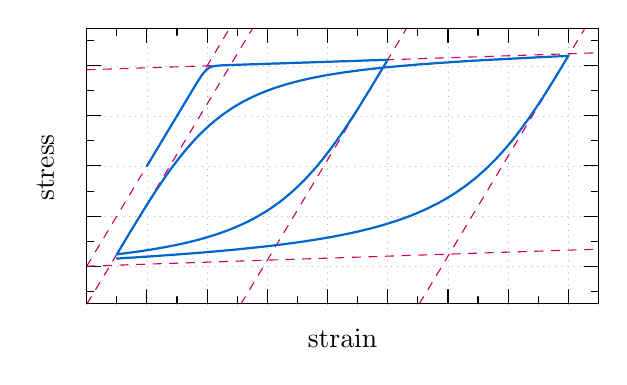
\begin{tikzpicture}[gnuplot]
%% generated with GNUPLOT 5.2p6 (Lua 5.3; terminal rev. Nov 2018, script rev. 107)
%% 03/05/2019 03:30:10
\path (0.000,0.000) rectangle (6.500,3.500);
\gpcolor{color=gp lt color border}
\gpsetlinetype{gp lt border}
\gpsetdashtype{gp dt solid}
\gpsetlinewidth{1.00}
\draw[gp path] (0.000,0.159)--(0.090,0.159);
\draw[gp path] (6.499,0.159)--(6.409,0.159);
\gpcolor{color=gp lt color axes}
\gpsetlinetype{gp lt axes}
\gpsetdashtype{gp dt axes}
\gpsetlinewidth{0.50}
\draw[gp path] (0.000,0.477)--(6.499,0.477);
\gpcolor{color=gp lt color border}
\gpsetlinetype{gp lt border}
\gpsetdashtype{gp dt solid}
\gpsetlinewidth{1.00}
\draw[gp path] (0.000,0.477)--(0.180,0.477);
\draw[gp path] (6.499,0.477)--(6.319,0.477);
\draw[gp path] (0.000,0.795)--(0.090,0.795);
\draw[gp path] (6.499,0.795)--(6.409,0.795);
\gpcolor{color=gp lt color axes}
\gpsetlinetype{gp lt axes}
\gpsetdashtype{gp dt axes}
\gpsetlinewidth{0.50}
\draw[gp path] (0.000,1.113)--(6.499,1.113);
\gpcolor{color=gp lt color border}
\gpsetlinetype{gp lt border}
\gpsetdashtype{gp dt solid}
\gpsetlinewidth{1.00}
\draw[gp path] (0.000,1.113)--(0.180,1.113);
\draw[gp path] (6.499,1.113)--(6.319,1.113);
\draw[gp path] (0.000,1.431)--(0.090,1.431);
\draw[gp path] (6.499,1.431)--(6.409,1.431);
\gpcolor{color=gp lt color axes}
\gpsetlinetype{gp lt axes}
\gpsetdashtype{gp dt axes}
\gpsetlinewidth{0.50}
\draw[gp path] (0.000,1.750)--(6.499,1.750);
\gpcolor{color=gp lt color border}
\gpsetlinetype{gp lt border}
\gpsetdashtype{gp dt solid}
\gpsetlinewidth{1.00}
\draw[gp path] (0.000,1.750)--(0.180,1.750);
\draw[gp path] (6.499,1.750)--(6.319,1.750);
\draw[gp path] (0.000,2.068)--(0.090,2.068);
\draw[gp path] (6.499,2.068)--(6.409,2.068);
\gpcolor{color=gp lt color axes}
\gpsetlinetype{gp lt axes}
\gpsetdashtype{gp dt axes}
\gpsetlinewidth{0.50}
\draw[gp path] (0.000,2.386)--(6.499,2.386);
\gpcolor{color=gp lt color border}
\gpsetlinetype{gp lt border}
\gpsetdashtype{gp dt solid}
\gpsetlinewidth{1.00}
\draw[gp path] (0.000,2.386)--(0.180,2.386);
\draw[gp path] (6.499,2.386)--(6.319,2.386);
\draw[gp path] (0.000,2.704)--(0.090,2.704);
\draw[gp path] (6.499,2.704)--(6.409,2.704);
\gpcolor{color=gp lt color axes}
\gpsetlinetype{gp lt axes}
\gpsetdashtype{gp dt axes}
\gpsetlinewidth{0.50}
\draw[gp path] (0.000,3.022)--(6.499,3.022);
\gpcolor{color=gp lt color border}
\gpsetlinetype{gp lt border}
\gpsetdashtype{gp dt solid}
\gpsetlinewidth{1.00}
\draw[gp path] (0.000,3.022)--(0.180,3.022);
\draw[gp path] (6.499,3.022)--(6.319,3.022);
\draw[gp path] (0.000,3.340)--(0.090,3.340);
\draw[gp path] (6.499,3.340)--(6.409,3.340);
\gpcolor{color=gp lt color axes}
\gpsetlinetype{gp lt axes}
\gpsetdashtype{gp dt axes}
\gpsetlinewidth{0.50}
\draw[gp path] (0.000,0.000)--(0.000,3.499);
\gpcolor{color=gp lt color border}
\gpsetlinetype{gp lt border}
\gpsetdashtype{gp dt solid}
\gpsetlinewidth{1.00}
\draw[gp path] (0.000,0.000)--(0.000,0.180);
\draw[gp path] (0.000,3.499)--(0.000,3.319);
\draw[gp path] (0.382,0.000)--(0.382,0.090);
\draw[gp path] (0.382,3.499)--(0.382,3.409);
\gpcolor{color=gp lt color axes}
\gpsetlinetype{gp lt axes}
\gpsetdashtype{gp dt axes}
\gpsetlinewidth{0.50}
\draw[gp path] (0.765,0.000)--(0.765,3.499);
\gpcolor{color=gp lt color border}
\gpsetlinetype{gp lt border}
\gpsetdashtype{gp dt solid}
\gpsetlinewidth{1.00}
\draw[gp path] (0.765,0.000)--(0.765,0.180);
\draw[gp path] (0.765,3.499)--(0.765,3.319);
\draw[gp path] (1.147,0.000)--(1.147,0.090);
\draw[gp path] (1.147,3.499)--(1.147,3.409);
\gpcolor{color=gp lt color axes}
\gpsetlinetype{gp lt axes}
\gpsetdashtype{gp dt axes}
\gpsetlinewidth{0.50}
\draw[gp path] (1.529,0.000)--(1.529,3.499);
\gpcolor{color=gp lt color border}
\gpsetlinetype{gp lt border}
\gpsetdashtype{gp dt solid}
\gpsetlinewidth{1.00}
\draw[gp path] (1.529,0.000)--(1.529,0.180);
\draw[gp path] (1.529,3.499)--(1.529,3.319);
\draw[gp path] (1.911,0.000)--(1.911,0.090);
\draw[gp path] (1.911,3.499)--(1.911,3.409);
\gpcolor{color=gp lt color axes}
\gpsetlinetype{gp lt axes}
\gpsetdashtype{gp dt axes}
\gpsetlinewidth{0.50}
\draw[gp path] (2.294,0.000)--(2.294,3.499);
\gpcolor{color=gp lt color border}
\gpsetlinetype{gp lt border}
\gpsetdashtype{gp dt solid}
\gpsetlinewidth{1.00}
\draw[gp path] (2.294,0.000)--(2.294,0.180);
\draw[gp path] (2.294,3.499)--(2.294,3.319);
\draw[gp path] (2.676,0.000)--(2.676,0.090);
\draw[gp path] (2.676,3.499)--(2.676,3.409);
\gpcolor{color=gp lt color axes}
\gpsetlinetype{gp lt axes}
\gpsetdashtype{gp dt axes}
\gpsetlinewidth{0.50}
\draw[gp path] (3.058,0.000)--(3.058,3.499);
\gpcolor{color=gp lt color border}
\gpsetlinetype{gp lt border}
\gpsetdashtype{gp dt solid}
\gpsetlinewidth{1.00}
\draw[gp path] (3.058,0.000)--(3.058,0.180);
\draw[gp path] (3.058,3.499)--(3.058,3.319);
\draw[gp path] (3.441,0.000)--(3.441,0.090);
\draw[gp path] (3.441,3.499)--(3.441,3.409);
\gpcolor{color=gp lt color axes}
\gpsetlinetype{gp lt axes}
\gpsetdashtype{gp dt axes}
\gpsetlinewidth{0.50}
\draw[gp path] (3.823,0.000)--(3.823,3.499);
\gpcolor{color=gp lt color border}
\gpsetlinetype{gp lt border}
\gpsetdashtype{gp dt solid}
\gpsetlinewidth{1.00}
\draw[gp path] (3.823,0.000)--(3.823,0.180);
\draw[gp path] (3.823,3.499)--(3.823,3.319);
\draw[gp path] (4.205,0.000)--(4.205,0.090);
\draw[gp path] (4.205,3.499)--(4.205,3.409);
\gpcolor{color=gp lt color axes}
\gpsetlinetype{gp lt axes}
\gpsetdashtype{gp dt axes}
\gpsetlinewidth{0.50}
\draw[gp path] (4.588,0.000)--(4.588,3.499);
\gpcolor{color=gp lt color border}
\gpsetlinetype{gp lt border}
\gpsetdashtype{gp dt solid}
\gpsetlinewidth{1.00}
\draw[gp path] (4.588,0.000)--(4.588,0.180);
\draw[gp path] (4.588,3.499)--(4.588,3.319);
\draw[gp path] (4.970,0.000)--(4.970,0.090);
\draw[gp path] (4.970,3.499)--(4.970,3.409);
\gpcolor{color=gp lt color axes}
\gpsetlinetype{gp lt axes}
\gpsetdashtype{gp dt axes}
\gpsetlinewidth{0.50}
\draw[gp path] (5.352,0.000)--(5.352,3.499);
\gpcolor{color=gp lt color border}
\gpsetlinetype{gp lt border}
\gpsetdashtype{gp dt solid}
\gpsetlinewidth{1.00}
\draw[gp path] (5.352,0.000)--(5.352,0.180);
\draw[gp path] (5.352,3.499)--(5.352,3.319);
\draw[gp path] (5.734,0.000)--(5.734,0.090);
\draw[gp path] (5.734,3.499)--(5.734,3.409);
\gpcolor{color=gp lt color axes}
\gpsetlinetype{gp lt axes}
\gpsetdashtype{gp dt axes}
\gpsetlinewidth{0.50}
\draw[gp path] (6.117,0.000)--(6.117,3.499);
\gpcolor{color=gp lt color border}
\gpsetlinetype{gp lt border}
\gpsetdashtype{gp dt solid}
\gpsetlinewidth{1.00}
\draw[gp path] (6.117,0.000)--(6.117,0.180);
\draw[gp path] (6.117,3.499)--(6.117,3.319);
\draw[gp path] (6.499,0.000)--(6.499,0.090);
\draw[gp path] (6.499,3.499)--(6.499,3.409);
\draw[gp path] (0.000,3.499)--(0.000,0.000)--(6.499,0.000)--(6.499,3.499)--cycle;
\node[gp node center,rotate=-270] at (-0.492,1.749) {stress};
\node[gp node center] at (3.249,-0.461) {strain};
\gpcolor{rgb color={0.800,0.000,0.400}}
\gpsetdashtype{gp dt 2}
\draw[gp path] (0.000,0.477)--(0.066,0.586)--(0.131,0.696)--(0.197,0.805)--(0.263,0.914)%
  --(0.328,1.023)--(0.394,1.133)--(0.460,1.242)--(0.525,1.351)--(0.591,1.460)--(0.656,1.570)%
  --(0.722,1.679)--(0.788,1.788)--(0.853,1.897)--(0.919,2.007)--(0.985,2.116)--(1.050,2.225)%
  --(1.116,2.334)--(1.182,2.444)--(1.247,2.553)--(1.313,2.662)--(1.379,2.771)--(1.444,2.880)%
  --(1.510,2.990)--(1.576,3.099)--(1.641,3.208)--(1.707,3.317)--(1.772,3.427)--(1.815,3.499);
\draw[gp path] (0.000,2.971)--(0.066,2.973)--(0.131,2.975)--(0.197,2.978)--(0.263,2.980)%
  --(0.328,2.982)--(0.394,2.984)--(0.460,2.986)--(0.525,2.988)--(0.591,2.991)--(0.656,2.993)%
  --(0.722,2.995)--(0.788,2.997)--(0.853,2.999)--(0.919,3.002)--(0.985,3.004)--(1.050,3.006)%
  --(1.116,3.008)--(1.182,3.010)--(1.247,3.012)--(1.313,3.015)--(1.379,3.017)--(1.444,3.019)%
  --(1.510,3.021)--(1.576,3.023)--(1.641,3.026)--(1.707,3.028)--(1.772,3.030)--(1.838,3.032)%
  --(1.904,3.034)--(1.969,3.037)--(2.035,3.039)--(2.101,3.041)--(2.166,3.043)--(2.232,3.045)%
  --(2.298,3.047)--(2.363,3.050)--(2.429,3.052)--(2.495,3.054)--(2.560,3.056)--(2.626,3.058)%
  --(2.692,3.061)--(2.757,3.063)--(2.823,3.065)--(2.888,3.067)--(2.954,3.069)--(3.020,3.071)%
  --(3.085,3.074)--(3.151,3.076)--(3.217,3.078)--(3.282,3.080)--(3.348,3.082)--(3.414,3.085)%
  --(3.479,3.087)--(3.545,3.089)--(3.611,3.091)--(3.676,3.093)--(3.742,3.096)--(3.807,3.098)%
  --(3.873,3.100)--(3.939,3.102)--(4.004,3.104)--(4.070,3.106)--(4.136,3.109)--(4.201,3.111)%
  --(4.267,3.113)--(4.333,3.115)--(4.398,3.117)--(4.464,3.120)--(4.530,3.122)--(4.595,3.124)%
  --(4.661,3.126)--(4.727,3.128)--(4.792,3.130)--(4.858,3.133)--(4.923,3.135)--(4.989,3.137)%
  --(5.055,3.139)--(5.120,3.141)--(5.186,3.144)--(5.252,3.146)--(5.317,3.148)--(5.383,3.150)%
  --(5.449,3.152)--(5.514,3.154)--(5.580,3.157)--(5.646,3.159)--(5.711,3.161)--(5.777,3.163)%
  --(5.843,3.165)--(5.908,3.168)--(5.974,3.170)--(6.039,3.172)--(6.105,3.174)--(6.171,3.176)%
  --(6.236,3.179)--(6.302,3.181)--(6.368,3.183)--(6.433,3.185)--(6.499,3.187);
\draw[gp path] (0.000,0.477)--(0.066,0.479)--(0.131,0.482)--(0.197,0.484)--(0.263,0.486)%
  --(0.328,0.488)--(0.394,0.490)--(0.460,0.492)--(0.525,0.495)--(0.591,0.497)--(0.656,0.499)%
  --(0.722,0.501)--(0.788,0.503)--(0.853,0.506)--(0.919,0.508)--(0.985,0.510)--(1.050,0.512)%
  --(1.116,0.514)--(1.182,0.516)--(1.247,0.519)--(1.313,0.521)--(1.379,0.523)--(1.444,0.525)%
  --(1.510,0.527)--(1.576,0.530)--(1.641,0.532)--(1.707,0.534)--(1.772,0.536)--(1.838,0.538)%
  --(1.904,0.540)--(1.969,0.543)--(2.035,0.545)--(2.101,0.547)--(2.166,0.549)--(2.232,0.551)%
  --(2.298,0.554)--(2.363,0.556)--(2.429,0.558)--(2.495,0.560)--(2.560,0.562)--(2.626,0.565)%
  --(2.692,0.567)--(2.757,0.569)--(2.823,0.571)--(2.888,0.573)--(2.954,0.575)--(3.020,0.578)%
  --(3.085,0.580)--(3.151,0.582)--(3.217,0.584)--(3.282,0.586)--(3.348,0.589)--(3.414,0.591)%
  --(3.479,0.593)--(3.545,0.595)--(3.611,0.597)--(3.676,0.599)--(3.742,0.602)--(3.807,0.604)%
  --(3.873,0.606)--(3.939,0.608)--(4.004,0.610)--(4.070,0.613)--(4.136,0.615)--(4.201,0.617)%
  --(4.267,0.619)--(4.333,0.621)--(4.398,0.624)--(4.464,0.626)--(4.530,0.628)--(4.595,0.630)%
  --(4.661,0.632)--(4.727,0.634)--(4.792,0.637)--(4.858,0.639)--(4.923,0.641)--(4.989,0.643)%
  --(5.055,0.645)--(5.120,0.648)--(5.186,0.650)--(5.252,0.652)--(5.317,0.654)--(5.383,0.656)%
  --(5.449,0.658)--(5.514,0.661)--(5.580,0.663)--(5.646,0.665)--(5.711,0.667)--(5.777,0.669)%
  --(5.843,0.672)--(5.908,0.674)--(5.974,0.676)--(6.039,0.678)--(6.105,0.680)--(6.171,0.683)%
  --(6.236,0.685)--(6.302,0.687)--(6.368,0.689)--(6.433,0.691)--(6.499,0.693);
\draw[gp path] (1.960,0.000)--(1.969,0.014)--(2.035,0.123)--(2.101,0.232)--(2.166,0.341)%
  --(2.232,0.451)--(2.298,0.560)--(2.363,0.669)--(2.429,0.778)--(2.495,0.888)--(2.560,0.997)%
  --(2.626,1.106)--(2.692,1.215)--(2.757,1.325)--(2.823,1.434)--(2.888,1.543)--(2.954,1.652)%
  --(3.020,1.762)--(3.085,1.871)--(3.151,1.980)--(3.217,2.089)--(3.282,2.199)--(3.348,2.308)%
  --(3.414,2.417)--(3.479,2.526)--(3.545,2.636)--(3.611,2.745)--(3.676,2.854)--(3.742,2.963)%
  --(3.807,3.073)--(3.873,3.182)--(3.939,3.291)--(4.004,3.400)--(4.063,3.499);
\draw[gp path] (0.004,0.000)--(0.066,0.101)--(0.131,0.210)--(0.197,0.319)--(0.263,0.429)%
  --(0.328,0.538)--(0.394,0.647)--(0.460,0.756)--(0.525,0.866)--(0.591,0.975)--(0.656,1.084)%
  --(0.722,1.193)--(0.788,1.302)--(0.853,1.412)--(0.919,1.521)--(0.985,1.630)--(1.050,1.739)%
  --(1.116,1.849)--(1.182,1.958)--(1.247,2.067)--(1.313,2.176)--(1.379,2.286)--(1.444,2.395)%
  --(1.510,2.504)--(1.576,2.613)--(1.641,2.723)--(1.707,2.832)--(1.772,2.941)--(1.838,3.050)%
  --(1.904,3.160)--(1.969,3.269)--(2.035,3.378)--(2.101,3.487)--(2.108,3.499);
\draw[gp path] (4.224,0.000)--(4.267,0.069)--(4.333,0.179)--(4.398,0.288)--(4.464,0.397)%
  --(4.530,0.506)--(4.595,0.616)--(4.661,0.725)--(4.727,0.834)--(4.792,0.943)--(4.858,1.053)%
  --(4.923,1.162)--(4.989,1.271)--(5.055,1.380)--(5.120,1.490)--(5.186,1.599)--(5.252,1.708)%
  --(5.317,1.817)--(5.383,1.927)--(5.449,2.036)--(5.514,2.145)--(5.580,2.254)--(5.646,2.364)%
  --(5.711,2.473)--(5.777,2.582)--(5.843,2.691)--(5.908,2.800)--(5.974,2.910)--(6.039,3.019)%
  --(6.105,3.128)--(6.171,3.237)--(6.236,3.347)--(6.302,3.456)--(6.328,3.499);
\gpcolor{rgb color={0.000,0.400,0.800}}
\gpsetdashtype{gp dt solid}
\gpsetlinewidth{2.00}
\draw[gp path] (0.765,1.750)--(0.803,1.813)--(0.841,1.877)--(0.879,1.940)--(0.918,2.004)%
  --(0.956,2.068)--(0.994,2.131)--(1.032,2.195)--(1.070,2.258)--(1.109,2.322)--(1.147,2.386)%
  --(1.185,2.449)--(1.223,2.513)--(1.262,2.577)--(1.300,2.640)--(1.338,2.704)--(1.376,2.767)%
  --(1.414,2.829)--(1.453,2.888)--(1.491,2.940)--(1.529,2.979)--(1.567,3.003)--(1.606,3.016)%
  --(1.644,3.022)--(1.682,3.025)--(1.720,3.028)--(1.759,3.029)--(1.797,3.031)--(1.835,3.032)%
  --(1.873,3.033)--(1.911,3.035)--(1.950,3.036)--(1.988,3.037)--(2.026,3.038)--(2.064,3.040)%
  --(2.103,3.041)--(2.141,3.042)--(2.179,3.043)--(2.217,3.045)--(2.256,3.046)--(2.294,3.047)%
  --(2.332,3.049)--(2.370,3.050)--(2.408,3.051)--(2.447,3.052)--(2.485,3.054)--(2.523,3.055)%
  --(2.561,3.056)--(2.600,3.057)--(2.638,3.059)--(2.676,3.060)--(2.714,3.061)--(2.753,3.063)%
  --(2.791,3.064)--(2.829,3.065)--(2.867,3.066)--(2.905,3.068)--(2.944,3.069)--(2.982,3.070)%
  --(3.020,3.071)--(3.058,3.073)--(3.097,3.074)--(3.135,3.075)--(3.173,3.077)--(3.211,3.078)%
  --(3.250,3.079)--(3.288,3.080)--(3.326,3.082)--(3.364,3.083)--(3.402,3.084)--(3.441,3.085)%
  --(3.479,3.087)--(3.517,3.088)--(3.555,3.089)--(3.594,3.091)--(3.632,3.092)--(3.670,3.093)%
  --(3.708,3.094)--(3.746,3.096)--(3.785,3.097)--(3.823,3.098)--(3.785,3.035)--(3.746,2.971)%
  --(3.708,2.908)--(3.670,2.844)--(3.632,2.781)--(3.594,2.718)--(3.555,2.656)--(3.517,2.594)%
  --(3.479,2.532)--(3.441,2.471)--(3.402,2.411)--(3.364,2.352)--(3.326,2.294)--(3.288,2.236)%
  --(3.250,2.180)--(3.211,2.124)--(3.173,2.070)--(3.135,2.017)--(3.097,1.965)--(3.058,1.915)%
  --(3.020,1.865)--(2.982,1.817)--(2.944,1.771)--(2.905,1.726)--(2.867,1.682)--(2.829,1.640)%
  --(2.791,1.599)--(2.753,1.559)--(2.714,1.521)--(2.676,1.484)--(2.638,1.449)--(2.600,1.415)%
  --(2.561,1.382)--(2.523,1.350)--(2.485,1.319)--(2.447,1.290)--(2.408,1.262)--(2.370,1.235)%
  --(2.332,1.208)--(2.294,1.183)--(2.256,1.159)--(2.217,1.136)--(2.179,1.114)--(2.141,1.093)%
  --(2.103,1.072)--(2.064,1.052)--(2.026,1.033)--(1.988,1.015)--(1.950,0.998)--(1.911,0.981)%
  --(1.873,0.965)--(1.835,0.949)--(1.797,0.934)--(1.759,0.920)--(1.720,0.906)--(1.682,0.893)%
  --(1.644,0.880)--(1.606,0.868)--(1.567,0.856)--(1.529,0.844)--(1.491,0.833)--(1.453,0.822)%
  --(1.414,0.812)--(1.376,0.802)--(1.338,0.792)--(1.300,0.783)--(1.262,0.774)--(1.223,0.765)%
  --(1.185,0.757)--(1.147,0.749)--(1.109,0.741)--(1.070,0.733)--(1.032,0.726)--(0.994,0.719)%
  --(0.956,0.712)--(0.918,0.705)--(0.879,0.698)--(0.841,0.692)--(0.803,0.686)--(0.765,0.680)%
  --(0.726,0.674)--(0.688,0.668)--(0.650,0.663)--(0.612,0.657)--(0.573,0.652)--(0.535,0.647)%
  --(0.497,0.642)--(0.459,0.637)--(0.421,0.632)--(0.382,0.628)--(0.421,0.691)--(0.459,0.755)%
  --(0.497,0.818)--(0.535,0.882)--(0.573,0.945)--(0.612,1.008)--(0.650,1.071)--(0.688,1.133)%
  --(0.726,1.195)--(0.765,1.256)--(0.803,1.316)--(0.841,1.376)--(0.879,1.435)--(0.918,1.493)%
  --(0.956,1.549)--(0.994,1.605)--(1.032,1.659)--(1.070,1.713)--(1.109,1.764)--(1.147,1.815)%
  --(1.185,1.864)--(1.223,1.911)--(1.262,1.958)--(1.300,2.002)--(1.338,2.045)--(1.376,2.087)%
  --(1.414,2.127)--(1.453,2.166)--(1.491,2.203)--(1.529,2.238)--(1.567,2.273)--(1.606,2.306)%
  --(1.644,2.337)--(1.682,2.367)--(1.720,2.396)--(1.759,2.424)--(1.797,2.450)--(1.835,2.476)%
  --(1.873,2.500)--(1.911,2.523)--(1.950,2.545)--(1.988,2.567)--(2.026,2.587)--(2.064,2.606)%
  --(2.103,2.625)--(2.141,2.642)--(2.179,2.659)--(2.217,2.676)--(2.256,2.691)--(2.294,2.706)%
  --(2.332,2.720)--(2.370,2.734)--(2.408,2.747)--(2.447,2.759)--(2.485,2.771)--(2.523,2.783)%
  --(2.561,2.794)--(2.600,2.804)--(2.638,2.815)--(2.676,2.824)--(2.714,2.834)--(2.753,2.843)%
  --(2.791,2.852)--(2.829,2.860)--(2.867,2.868)--(2.905,2.876)--(2.944,2.883)--(2.982,2.891)%
  --(3.020,2.898)--(3.058,2.904)--(3.097,2.911)--(3.135,2.917)--(3.173,2.923)--(3.211,2.929)%
  --(3.250,2.935)--(3.288,2.941)--(3.326,2.946)--(3.364,2.951)--(3.402,2.956)--(3.441,2.961)%
  --(3.479,2.966)--(3.517,2.971)--(3.555,2.975)--(3.594,2.980)--(3.632,2.984)--(3.670,2.988)%
  --(3.708,2.992)--(3.746,2.996)--(3.785,3.000)--(3.823,3.004)--(3.861,3.008)--(3.899,3.011)%
  --(3.938,3.015)--(3.976,3.018)--(4.014,3.022)--(4.052,3.025)--(4.091,3.028)--(4.129,3.031)%
  --(4.167,3.035)--(4.205,3.038)--(4.243,3.041)--(4.282,3.044)--(4.320,3.046)--(4.358,3.049)%
  --(4.396,3.052)--(4.435,3.055)--(4.473,3.058)--(4.511,3.060)--(4.549,3.063)--(4.588,3.065)%
  --(4.626,3.068)--(4.664,3.071)--(4.702,3.073)--(4.740,3.075)--(4.779,3.078)--(4.817,3.080)%
  --(4.855,3.083)--(4.893,3.085)--(4.932,3.087)--(4.970,3.089)--(5.008,3.092)--(5.046,3.094)%
  --(5.085,3.096)--(5.123,3.098)--(5.161,3.100)--(5.199,3.102)--(5.237,3.104)--(5.276,3.106)%
  --(5.314,3.108)--(5.352,3.111)--(5.390,3.112)--(5.429,3.114)--(5.467,3.116)--(5.505,3.118)%
  --(5.543,3.120)--(5.581,3.122)--(5.620,3.124)--(5.658,3.126)--(5.696,3.128)--(5.734,3.130)%
  --(5.773,3.132)--(5.811,3.133)--(5.849,3.135)--(5.887,3.137)--(5.926,3.139)--(5.964,3.141)%
  --(6.002,3.142)--(6.040,3.144)--(6.078,3.146)--(6.117,3.148)--(6.078,3.084)--(6.040,3.020)%
  --(6.002,2.957)--(5.964,2.894)--(5.926,2.832)--(5.887,2.770)--(5.849,2.709)--(5.811,2.649)%
  --(5.773,2.589)--(5.734,2.531)--(5.696,2.474)--(5.658,2.417)--(5.620,2.362)--(5.581,2.308)%
  --(5.543,2.255)--(5.505,2.204)--(5.467,2.154)--(5.429,2.105)--(5.390,2.058)--(5.352,2.012)%
  --(5.314,1.967)--(5.276,1.924)--(5.237,1.882)--(5.199,1.841)--(5.161,1.802)--(5.123,1.764)%
  --(5.085,1.727)--(5.046,1.691)--(5.008,1.657)--(4.970,1.623)--(4.932,1.591)--(4.893,1.560)%
  --(4.855,1.530)--(4.817,1.502)--(4.779,1.474)--(4.740,1.447)--(4.702,1.421)--(4.664,1.396)%
  --(4.626,1.372)--(4.588,1.348)--(4.549,1.326)--(4.511,1.304)--(4.473,1.283)--(4.435,1.263)%
  --(4.396,1.244)--(4.358,1.225)--(4.320,1.206)--(4.282,1.189)--(4.243,1.172)--(4.205,1.155)%
  --(4.167,1.140)--(4.129,1.124)--(4.091,1.109)--(4.052,1.095)--(4.014,1.081)--(3.976,1.067)%
  --(3.938,1.054)--(3.899,1.042)--(3.861,1.030)--(3.823,1.018)--(3.785,1.006)--(3.746,0.995)%
  --(3.708,0.984)--(3.670,0.974)--(3.632,0.963)--(3.594,0.953)--(3.555,0.944)--(3.517,0.934)%
  --(3.479,0.925)--(3.441,0.916)--(3.402,0.908)--(3.364,0.899)--(3.326,0.891)--(3.288,0.883)%
  --(3.250,0.876)--(3.211,0.868)--(3.173,0.861)--(3.135,0.853)--(3.097,0.846)--(3.058,0.840)%
  --(3.020,0.833)--(2.982,0.826)--(2.944,0.820)--(2.905,0.814)--(2.867,0.808)--(2.829,0.802)%
  --(2.791,0.796)--(2.753,0.790)--(2.714,0.785)--(2.676,0.779)--(2.638,0.774)--(2.600,0.769)%
  --(2.561,0.764)--(2.523,0.759)--(2.485,0.754)--(2.447,0.749)--(2.408,0.744)--(2.370,0.740)%
  --(2.332,0.735)--(2.294,0.731)--(2.256,0.726)--(2.217,0.722)--(2.179,0.718)--(2.141,0.714)%
  --(2.103,0.710)--(2.064,0.706)--(2.026,0.702)--(1.988,0.698)--(1.950,0.694)--(1.911,0.690)%
  --(1.873,0.686)--(1.835,0.683)--(1.797,0.679)--(1.759,0.676)--(1.720,0.672)--(1.682,0.669)%
  --(1.644,0.665)--(1.606,0.662)--(1.567,0.659)--(1.529,0.656)--(1.491,0.652)--(1.453,0.649)%
  --(1.414,0.646)--(1.376,0.643)--(1.338,0.640)--(1.300,0.637)--(1.262,0.634)--(1.223,0.631)%
  --(1.185,0.628)--(1.147,0.625)--(1.109,0.623)--(1.070,0.620)--(1.032,0.617)--(0.994,0.614)%
  --(0.956,0.612)--(0.918,0.609)--(0.879,0.606)--(0.841,0.604)--(0.803,0.601)--(0.765,0.598)%
  --(0.726,0.596)--(0.688,0.593)--(0.650,0.591)--(0.612,0.588)--(0.573,0.586)--(0.535,0.584)%
  --(0.497,0.581)--(0.459,0.579)--(0.421,0.576)--(0.382,0.574);
\gpcolor{color=gp lt color border}
\gpsetlinewidth{1.00}
\draw[gp path] (0.000,3.499)--(0.000,0.000)--(6.499,0.000)--(6.499,3.499)--cycle;
%% coordinates of the plot area
\gpdefrectangularnode{gp plot 1}{\pgfpoint{0.000cm}{0.000cm}}{\pgfpoint{6.499cm}{3.499cm}}
\end{tikzpicture}
%% gnuplot variables

\caption{steel model}\label{fig:steel}
\end{subfigure}
\caption{schematic sketches of the material models used in analyses}\label{fig:material}
\end{figure}

In this work, reinforcement is modelled independently in a smeared approach. Hence interactions between reinforcement and host concrete, such as dowel action, bar buckling and confinement, are not considered (not in an discrete way but still can be accounted for by modifying material models). The total material stiffness $\mathbold{D}$ and stress $\mathbold{\sigma}$ can be expressed as the superposition of concrete and reinforcement response.
\begin{gather}
\mathbold{D}=\mathbold{D}_c+\mathbold{D}_s,\quad
\mathbold{\sigma}=\mathbold{\sigma}_c+\mathbold{\sigma}_s,
\end{gather}
where $\mathbold{D}$ is the overall material stiffness, subscripts $_c$ and $_s$ denote concrete and reinforcement portion, respectively. $\mathbold{D}_s$ is often assumed to be orthogonal so that
\begin{gather}
\mathbold{D}_s=\begin{bmatrix}
	\rho_xE_x & 0         & 0 \\
	0         & \rho_yE_y & 0 \\
	0         & 0         & 0
\end{bmatrix},\quad
\mathbold{\sigma}_s=\begin{bmatrix}
	\rho_x\sigma_x \\
	\rho_y\sigma_y \\
	0
\end{bmatrix},
\end{gather}
where $\rho_x$ and $\rho_y$ are two reinforcement ratios along two axes, $E_x$ and $E_y$ are corresponding steel moduli. Both the main reinforcement and stirrups along the two perpendicular directions can be considered. It shall be stressed that, although the smeared approach is used, GCMQ itself does not impose any constraint on the implementation of reinforcement. The discrete approach, or a combined method, could be employed as well.
\section{Numerical Simulations}
\subsection{Plain Concrete Panel}
A plain concrete panel with a unit size is used with the CDP model to showcase the performance baseline of GCMQ. The panel is fully fixed at one end and a uniform shear deformation is applied at the other end. Noting that strength degradation tends to be mesh dependent, which is known due to the size effect \citep[see, e.g.,][]{Bazant1983}, normalised fracture energy $g_t$ and its counterpart $g_c$, are strictly scaled according to their original definitions \citep{Lubliner1989} as shown in \tabref{tab:sp_gtgc} so that mesh dependence can be largely eliminated.
\begin{table}[htbp]
\scriptsize\centering\caption{normalised energy adopted in plain concrete panel example}\label{tab:sp_gtgc}
\begin{tabular}{lllll}
	\toprule
	                                       &            \multicolumn{4}{c}{mesh grid}            \\
	                                       & \numproduct{1x1}  & \numproduct{2x2}  & \numproduct{4x4}   & \numproduct{8x8}   \\ \midrule
	$g_t$ (\si{\newton\per\milli\meter^2}) & \num{4E-3} & \num{8E-3} & \num{16E-3} & \num{32E-3} \\
	$g_c$ (\si{\newton\per\milli\meter^2}) & \num{4E-1} & \num{8E-1} & \num{16E-1} & \num{32E-1} \\ \bottomrule
\end{tabular}
\end{table}
Other parameters remain unchanged for different meshes. They are: elastic modulus $E=\SI{30}{\giga\pascal}$, Poisson's ratio $\nu=\num{0.2}$, tensile strength $f_t=\SI{4}{\mega\pascal}$, compressive strength $f_c=\SI{40}{\mega\pascal}$, tensile softening parameter $a_t=\num{0.2}$, compressive hardening paramater $a_c=\num{4.0}$, reference degradation factor at half tensile strength $\bar{D}_t=\num{0.6}$, reference degradation factor at compressive strength $\bar{D}_c=\num{0.6}$, dilatation parameter $\alpha_p=\num{0.2}$, ratio between biaxial and uniaxial compressive strengths $f_{bc}/f_c=\num{1.16}$. Details on explanations and definitions of those material properties is documented elsewhere \citep{Lubliner1989,Lee1996,Lee1998}.

The benchmark results are shown in \figref{fig:single_patch}. Numbers in brackets indicate mesh density. Three different integration schemes are tested, which are denoted with suffixes -I (5-point \citep{Irons1971}), -G (\numproduct{3x3} Gauss) and -L (\numproduct{3x3} Lobatto). With a \numproduct{2x2} mesh grid, GCMQ is able to predict an equivalently accurate response compared to that of Q4 (CPS4 in ABAQUS notation) element \citep{Taig1964} with an \numproduct{8x8} mesh grid.
\begin{figure}[htb]
\scriptsize\centering
\begin{subfigure}[b]{.48\textwidth}
\begin{tikzpicture}[gnuplot]
%% generated with GNUPLOT 5.2p6 (Lua 5.3; terminal rev. Nov 2018, script rev. 107)
%% 03/03/2019 17:40:10
\path (0.000,0.000) rectangle (6.500,4.000);
\gpcolor{color=gp lt color axes}
\gpsetlinetype{gp lt axes}
\gpsetdashtype{gp dt axes}
\gpsetlinewidth{0.50}
\draw[gp path] (0.000,0.000)--(6.499,0.000);
\gpcolor{color=gp lt color border}
\gpsetlinetype{gp lt border}
\gpsetdashtype{gp dt solid}
\gpsetlinewidth{1.00}
\draw[gp path] (0.000,0.000)--(0.180,0.000);
\node[gp node right] at (-0.184,0.000) {$0$};
\draw[gp path] (0.000,0.800)--(0.090,0.800);
\gpcolor{color=gp lt color axes}
\gpsetlinetype{gp lt axes}
\gpsetdashtype{gp dt axes}
\gpsetlinewidth{0.50}
\draw[gp path] (0.000,1.600)--(6.499,1.600);
\gpcolor{color=gp lt color border}
\gpsetlinetype{gp lt border}
\gpsetdashtype{gp dt solid}
\gpsetlinewidth{1.00}
\draw[gp path] (0.000,1.600)--(0.180,1.600);
\node[gp node right] at (-0.184,1.600) {$1$};
\draw[gp path] (0.000,2.399)--(0.090,2.399);
\gpcolor{color=gp lt color axes}
\gpsetlinetype{gp lt axes}
\gpsetdashtype{gp dt axes}
\gpsetlinewidth{0.50}
\draw[gp path] (0.000,3.199)--(6.499,3.199);
\gpcolor{color=gp lt color border}
\gpsetlinetype{gp lt border}
\gpsetdashtype{gp dt solid}
\gpsetlinewidth{1.00}
\draw[gp path] (0.000,3.199)--(0.180,3.199);
\node[gp node right] at (-0.184,3.199) {$2$};
\gpcolor{color=gp lt color axes}
\gpsetlinetype{gp lt axes}
\gpsetdashtype{gp dt axes}
\gpsetlinewidth{0.50}
\draw[gp path] (0.000,0.000)--(0.000,3.999);
\gpcolor{color=gp lt color border}
\gpsetlinetype{gp lt border}
\gpsetdashtype{gp dt solid}
\gpsetlinewidth{1.00}
\draw[gp path] (0.000,0.000)--(0.000,0.180);
\node[gp node center] at (0.000,-0.308) {$0$};
\draw[gp path] (0.812,0.000)--(0.812,0.090);
\gpcolor{color=gp lt color axes}
\gpsetlinetype{gp lt axes}
\gpsetdashtype{gp dt axes}
\gpsetlinewidth{0.50}
\draw[gp path] (1.625,0.000)--(1.625,0.300);
\draw[gp path] (1.625,1.532)--(1.625,3.999);
\gpcolor{color=gp lt color border}
\gpsetlinetype{gp lt border}
\gpsetdashtype{gp dt solid}
\gpsetlinewidth{1.00}
\draw[gp path] (1.625,0.000)--(1.625,0.180);
\node[gp node center] at (1.625,-0.308) {$0.5$};
\draw[gp path] (2.437,0.000)--(2.437,0.090);
\gpcolor{color=gp lt color axes}
\gpsetlinetype{gp lt axes}
\gpsetdashtype{gp dt axes}
\gpsetlinewidth{0.50}
\draw[gp path] (3.250,0.000)--(3.250,0.300);
\draw[gp path] (3.250,1.532)--(3.250,3.999);
\gpcolor{color=gp lt color border}
\gpsetlinetype{gp lt border}
\gpsetdashtype{gp dt solid}
\gpsetlinewidth{1.00}
\draw[gp path] (3.250,0.000)--(3.250,0.180);
\node[gp node center] at (3.250,-0.308) {$1$};
\draw[gp path] (4.062,0.000)--(4.062,0.090);
\gpcolor{color=gp lt color axes}
\gpsetlinetype{gp lt axes}
\gpsetdashtype{gp dt axes}
\gpsetlinewidth{0.50}
\draw[gp path] (4.874,0.000)--(4.874,3.999);
\gpcolor{color=gp lt color border}
\gpsetlinetype{gp lt border}
\gpsetdashtype{gp dt solid}
\gpsetlinewidth{1.00}
\draw[gp path] (4.874,0.000)--(4.874,0.180);
\node[gp node center] at (4.874,-0.308) {$1.5$};
\draw[gp path] (5.687,0.000)--(5.687,0.090);
\gpcolor{color=gp lt color axes}
\gpsetlinetype{gp lt axes}
\gpsetdashtype{gp dt axes}
\gpsetlinewidth{0.50}
\draw[gp path] (6.499,0.000)--(6.499,3.999);
\gpcolor{color=gp lt color border}
\gpsetlinetype{gp lt border}
\gpsetdashtype{gp dt solid}
\gpsetlinewidth{1.00}
\draw[gp path] (6.499,0.000)--(6.499,0.180);
\node[gp node center] at (6.499,-0.308) {$2$};
\draw[gp path] (0.000,3.999)--(0.000,0.000)--(6.499,0.000)--(6.499,3.999)--cycle;
\node[gp node center,rotate=-270] at (-0.676,1.999) {base resistance};
\node[gp node center] at (3.249,-0.769) {top displacement (\num{E-3})};
\node[gp node right] at (1.981,1.378) {Q4 (1)};
\gpcolor{rgb color={0.894,0.102,0.110}}
\gpsetlinewidth{2.00}
\draw[gp path] (2.165,1.378)--(2.437,1.378);
\draw[gp path] (0.000,0.000)--(0.065,0.215)--(0.130,0.431)--(0.195,0.646)--(0.260,0.861)%
  --(0.325,1.077)--(0.390,1.292)--(0.455,1.507)--(0.520,1.723)--(0.585,1.938)--(0.650,2.153)%
  --(0.715,2.369)--(0.780,2.584)--(0.845,2.745)--(0.910,2.868)--(0.975,2.984)--(1.040,3.108)%
  --(1.105,3.231)--(1.170,3.354)--(1.235,3.428)--(1.300,3.481)--(1.365,3.517)--(1.430,3.558)%
  --(1.495,3.595)--(1.560,3.619)--(1.625,3.606)--(1.690,3.594)--(1.755,3.583)--(1.820,3.571)%
  --(1.885,3.557)--(1.950,3.543)--(2.015,3.527)--(2.080,3.510)--(2.145,3.493)--(2.210,3.475)%
  --(2.275,3.456)--(2.340,3.436)--(2.405,3.415)--(2.470,3.394)--(2.535,3.372)--(2.600,3.349)%
  --(2.665,3.326)--(2.730,3.302)--(2.795,3.278)--(2.860,3.254)--(2.925,3.229)--(2.990,3.204)%
  --(3.055,3.179)--(3.120,3.153)--(3.185,3.127)--(3.250,3.101)--(3.314,3.075)--(3.379,3.049)%
  --(3.444,3.023)--(3.509,2.997)--(3.574,2.971)--(3.639,2.945)--(3.704,2.919)--(3.769,2.893)%
  --(3.834,2.868)--(3.899,2.842)--(3.964,2.818)--(4.029,2.793)--(4.094,2.769)--(4.159,2.745)%
  --(4.224,2.721)--(4.289,2.698)--(4.354,2.675)--(4.419,2.653)--(4.484,2.631)--(4.549,2.610)%
  --(4.614,2.589)--(4.679,2.569)--(4.744,2.549)--(4.809,2.530)--(4.874,2.511)--(4.939,2.492)%
  --(5.004,2.475)--(5.069,2.457)--(5.134,2.441)--(5.199,2.424)--(5.264,2.409)--(5.329,2.393)%
  --(5.394,2.378)--(5.459,2.364)--(5.524,2.350)--(5.589,2.336)--(5.654,2.323)--(5.719,2.311)%
  --(5.784,2.298)--(5.849,2.286)--(5.914,2.275)--(5.979,2.264)--(6.044,2.253)--(6.109,2.242)%
  --(6.174,2.232)--(6.239,2.222)--(6.304,2.213)--(6.369,2.203)--(6.434,2.194)--(6.499,2.186);
\gpsetpointsize{4.00}
\gppoint{gp mark 1}{(0.000,0.000)}
\gppoint{gp mark 1}{(0.715,2.369)}
\gppoint{gp mark 1}{(1.430,3.558)}
\gppoint{gp mark 1}{(2.145,3.493)}
\gppoint{gp mark 1}{(2.860,3.254)}
\gppoint{gp mark 1}{(3.574,2.971)}
\gppoint{gp mark 1}{(4.289,2.698)}
\gppoint{gp mark 1}{(5.004,2.475)}
\gppoint{gp mark 1}{(5.719,2.311)}
\gppoint{gp mark 1}{(6.434,2.194)}
\gppoint{gp mark 1}{(2.301,1.378)}
\gpcolor{color=gp lt color border}
\node[gp node right] at (1.981,1.070) {Q4 (2)};
\gpcolor{rgb color={0.216,0.494,0.722}}
\draw[gp path] (2.165,1.070)--(2.437,1.070);
\draw[gp path] (0.000,0.000)--(0.065,0.168)--(0.130,0.335)--(0.195,0.503)--(0.260,0.671)%
  --(0.325,0.839)--(0.390,1.006)--(0.455,1.174)--(0.520,1.342)--(0.585,1.510)--(0.650,1.664)%
  --(0.715,1.795)--(0.780,1.884)--(0.845,1.962)--(0.910,2.045)--(0.975,2.124)--(1.040,2.199)%
  --(1.105,2.256)--(1.170,2.310)--(1.235,2.364)--(1.300,2.420)--(1.365,2.465)--(1.430,2.495)%
  --(1.495,2.522)--(1.560,2.535)--(1.625,2.547)--(1.690,2.555)--(1.755,2.565)--(1.820,2.574)%
  --(1.885,2.582)--(1.950,2.589)--(2.015,2.596)--(2.080,2.603)--(2.145,2.610)--(2.210,2.617)%
  --(2.275,2.623)--(2.340,2.629)--(2.405,2.632)--(2.470,2.623)--(2.535,2.608)--(2.600,2.597)%
  --(2.665,2.580)--(2.730,2.564)--(2.795,2.538)--(2.860,2.516)--(2.925,2.493)--(2.990,2.470)%
  --(3.055,2.447)--(3.120,2.423)--(3.185,2.399)--(3.250,2.375)--(3.314,2.351)--(3.379,2.326)%
  --(3.444,2.302)--(3.509,2.277)--(3.574,2.252)--(3.639,2.227)--(3.704,2.203)--(3.769,2.179)%
  --(3.834,2.155)--(3.899,2.131)--(3.964,2.107)--(4.029,2.085)--(4.094,2.061)--(4.159,2.037)%
  --(4.224,2.013)--(4.289,1.990)--(4.354,1.967)--(4.419,1.943)--(4.484,1.920)--(4.549,1.898)%
  --(4.614,1.875)--(4.679,1.853)--(4.744,1.830)--(4.809,1.808)--(4.874,1.787)--(4.939,1.765)%
  --(5.004,1.744)--(5.069,1.723)--(5.134,1.702)--(5.199,1.681)--(5.264,1.661)--(5.329,1.641)%
  --(5.394,1.622)--(5.459,1.602)--(5.524,1.583)--(5.589,1.564)--(5.654,1.545)--(5.719,1.527)%
  --(5.784,1.509)--(5.849,1.491)--(5.914,1.474)--(5.979,1.456)--(6.044,1.439)--(6.109,1.423)%
  --(6.174,1.406)--(6.239,1.390)--(6.304,1.375)--(6.369,1.359)--(6.434,1.344)--(6.499,1.329);
\gppoint{gp mark 2}{(0.000,0.000)}
\gppoint{gp mark 2}{(1.105,2.256)}
\gppoint{gp mark 2}{(2.210,2.617)}
\gppoint{gp mark 2}{(3.314,2.351)}
\gppoint{gp mark 2}{(4.419,1.943)}
\gppoint{gp mark 2}{(5.524,1.583)}
\gppoint{gp mark 2}{(2.301,1.070)}
\gpcolor{color=gp lt color border}
\node[gp node right] at (1.981,0.762) {Q4 (4)};
\gpcolor{rgb color={0.302,0.686,0.290}}
\draw[gp path] (2.165,0.762)--(2.437,0.762);
\draw[gp path] (0.000,0.000)--(0.065,0.149)--(0.130,0.298)--(0.195,0.448)--(0.260,0.597)%
  --(0.325,0.746)--(0.390,0.895)--(0.455,1.044)--(0.520,1.193)--(0.585,1.317)--(0.650,1.430)%
  --(0.715,1.548)--(0.780,1.649)--(0.845,1.737)--(0.910,1.818)--(0.975,1.881)--(1.040,1.942)%
  --(1.105,1.994)--(1.170,2.045)--(1.235,2.085)--(1.300,2.125)--(1.365,2.167)--(1.430,2.185)%
  --(1.495,2.214)--(1.560,2.231)--(1.625,2.252)--(1.690,2.269)--(1.755,2.274)--(1.820,2.280)%
  --(1.885,2.288)--(1.950,2.286)--(2.015,2.286)--(2.080,2.287)--(2.145,2.286)--(2.210,2.284)%
  --(2.275,2.282)--(2.340,2.279)--(2.405,2.275)--(2.470,2.272)--(2.535,2.264)--(2.600,2.258)%
  --(2.665,2.253)--(2.730,2.247)--(2.795,2.231)--(2.860,2.218)--(2.925,2.206)--(2.990,2.192)%
  --(3.055,2.178)--(3.120,2.163)--(3.185,2.148)--(3.250,2.133)--(3.314,2.118)--(3.379,2.102)%
  --(3.444,2.087)--(3.509,2.071)--(3.574,2.056)--(3.639,2.040)--(3.704,2.025)--(3.769,2.009)%
  --(3.834,1.993)--(3.899,1.972)--(3.964,1.959)--(4.029,1.943)--(4.094,1.927)--(4.159,1.911)%
  --(4.224,1.895)--(4.289,1.879)--(4.354,1.863)--(4.419,1.847)--(4.484,1.827)--(4.549,1.806)%
  --(4.614,1.789)--(4.679,1.770)--(4.744,1.751)--(4.809,1.731)--(4.874,1.712)--(4.939,1.692)%
  --(5.004,1.673)--(5.069,1.654)--(5.134,1.634)--(5.199,1.616)--(5.264,1.597)--(5.329,1.578)%
  --(5.394,1.559)--(5.459,1.541)--(5.524,1.522)--(5.589,1.504)--(5.654,1.486)--(5.719,1.468)%
  --(5.784,1.450)--(5.849,1.433)--(5.914,1.415)--(5.979,1.398)--(6.044,1.381)--(6.109,1.364)%
  --(6.174,1.347)--(6.239,1.331)--(6.304,1.314)--(6.369,1.298)--(6.434,1.282)--(6.499,1.266);
\gppoint{gp mark 3}{(0.000,0.000)}
\gppoint{gp mark 3}{(1.495,2.214)}
\gppoint{gp mark 3}{(2.990,2.192)}
\gppoint{gp mark 3}{(4.484,1.827)}
\gppoint{gp mark 3}{(5.979,1.398)}
\gppoint{gp mark 3}{(2.301,0.762)}
\gpcolor{color=gp lt color border}
\node[gp node right] at (1.981,0.454) {Q4 (8)};
\gpcolor{rgb color={0.596,0.306,0.639}}
\draw[gp path] (2.165,0.454)--(2.437,0.454);
\draw[gp path] (0.000,0.000)--(0.065,0.144)--(0.130,0.288)--(0.195,0.431)--(0.260,0.575)%
  --(0.325,0.719)--(0.390,0.863)--(0.455,1.005)--(0.520,1.136)--(0.585,1.265)--(0.650,1.377)%
  --(0.715,1.474)--(0.780,1.578)--(0.845,1.658)--(0.910,1.731)--(0.975,1.803)--(1.040,1.866)%
  --(1.105,1.913)--(1.170,1.955)--(1.235,2.003)--(1.300,2.041)--(1.365,2.068)--(1.430,2.096)%
  --(1.495,2.118)--(1.560,2.143)--(1.625,2.155)--(1.690,2.177)--(1.755,2.192)--(1.820,2.197)%
  --(1.885,2.200)--(1.950,2.212)--(2.015,2.213)--(2.080,2.212)--(2.145,2.208)--(2.210,2.211)%
  --(2.275,2.209)--(2.340,2.206)--(2.405,2.197)--(2.470,2.194)--(2.535,2.188)--(2.600,2.182)%
  --(2.665,2.164)--(2.730,2.157)--(2.795,2.150)--(2.860,2.140)--(2.925,2.129)--(2.990,2.114)%
  --(3.055,2.096)--(3.120,2.084)--(3.185,2.071)--(3.250,2.056)--(3.314,2.041)--(3.379,2.026)%
  --(3.444,2.010)--(3.509,1.993)--(3.574,1.976)--(3.639,1.960)--(3.704,1.944)--(3.769,1.927)%
  --(3.834,1.910)--(3.899,1.893)--(3.964,1.876)--(4.029,1.856)--(4.094,1.840)--(4.159,1.823)%
  --(4.224,1.805)--(4.289,1.788)--(4.354,1.770)--(4.419,1.753)--(4.484,1.736)--(4.549,1.719)%
  --(4.614,1.702)--(4.679,1.683)--(4.744,1.663)--(4.809,1.648)--(4.874,1.631)--(4.939,1.614)%
  --(5.004,1.597)--(5.069,1.580)--(5.134,1.563)--(5.199,1.546)--(5.264,1.530)--(5.329,1.513)%
  --(5.394,1.497)--(5.459,1.481)--(5.524,1.465)--(5.589,1.449)--(5.654,1.433)--(5.719,1.418)%
  --(5.784,1.402)--(5.849,1.387)--(5.914,1.371)--(5.979,1.357)--(6.044,1.342)--(6.109,1.327)%
  --(6.174,1.313)--(6.239,1.298)--(6.304,1.284)--(6.369,1.270)--(6.434,1.256)--(6.499,1.242);
\gppoint{gp mark 4}{(0.000,0.000)}
\gppoint{gp mark 4}{(2.015,2.213)}
\gppoint{gp mark 4}{(4.029,1.856)}
\gppoint{gp mark 4}{(6.044,1.342)}
\gppoint{gp mark 4}{(2.301,0.454)}
\gpcolor{color=gp lt color border}
\node[gp node right] at (3.909,1.378) {-I (1)};
\gpcolor{rgb color={0.894,0.102,0.110}}
\draw[gp path] (4.093,1.378)--(4.365,1.378);
\draw[gp path] (0.000,0.000)--(0.065,0.178)--(0.130,0.355)--(0.195,0.533)--(0.260,0.711)%
  --(0.325,0.889)--(0.390,1.066)--(0.455,1.244)--(0.520,1.422)--(0.585,1.600)--(0.650,1.777)%
  --(0.715,1.934)--(0.780,2.001)--(0.845,2.057)--(0.910,2.111)--(0.975,2.160)--(1.040,2.199)%
  --(1.105,2.245)--(1.170,2.290)--(1.235,2.335)--(1.300,2.378)--(1.365,2.422)--(1.430,2.464)%
  --(1.495,2.506)--(1.560,2.548)--(1.625,2.590)--(1.690,2.632)--(1.755,2.673)--(1.820,2.715)%
  --(1.885,2.756)--(1.950,2.798)--(2.015,2.822)--(2.080,2.822)--(2.145,2.819)--(2.210,2.800)%
  --(2.275,2.779)--(2.340,2.758)--(2.405,2.737)--(2.470,2.716)--(2.535,2.695)--(2.600,2.675)%
  --(2.665,2.654)--(2.730,2.634)--(2.795,2.613)--(2.860,2.593)--(2.925,2.573)--(2.990,2.553)%
  --(3.055,2.533)--(3.120,2.514)--(3.185,2.494)--(3.250,2.475)--(3.314,2.456)--(3.379,2.436)%
  --(3.444,2.417)--(3.509,2.399)--(3.574,2.380)--(3.639,2.362)--(3.704,2.344)--(3.769,2.326)%
  --(3.834,2.308)--(3.899,2.290)--(3.964,2.272)--(4.029,2.255)--(4.094,2.237)--(4.159,2.220)%
  --(4.224,2.203)--(4.289,2.186)--(4.354,2.168)--(4.419,2.151)--(4.484,2.134)--(4.549,2.117)%
  --(4.614,2.100)--(4.679,2.083)--(4.744,2.066)--(4.809,2.049)--(4.874,2.032)--(4.939,2.015)%
  --(5.004,1.998)--(5.069,1.981)--(5.134,1.964)--(5.199,1.946)--(5.264,1.928)--(5.329,1.911)%
  --(5.394,1.893)--(5.459,1.876)--(5.524,1.858)--(5.589,1.840)--(5.654,1.821)--(5.719,1.803)%
  --(5.784,1.784)--(5.849,1.765)--(5.914,1.746)--(5.979,1.727)--(6.044,1.707)--(6.109,1.687)%
  --(6.174,1.667)--(6.239,1.646)--(6.304,1.625)--(6.369,1.604)--(6.434,1.582)--(6.499,1.560);
\gppoint{gp mark 5}{(0.000,0.000)}
\gppoint{gp mark 5}{(0.715,1.934)}
\gppoint{gp mark 5}{(1.430,2.464)}
\gppoint{gp mark 5}{(2.145,2.819)}
\gppoint{gp mark 5}{(2.860,2.593)}
\gppoint{gp mark 5}{(3.574,2.380)}
\gppoint{gp mark 5}{(4.289,2.186)}
\gppoint{gp mark 5}{(5.004,1.998)}
\gppoint{gp mark 5}{(5.719,1.803)}
\gppoint{gp mark 5}{(6.434,1.582)}
\gppoint{gp mark 5}{(4.229,1.378)}
\gpcolor{color=gp lt color border}
\node[gp node right] at (3.909,1.070) {-I (2)};
\gpcolor{rgb color={0.216,0.494,0.722}}
\draw[gp path] (4.093,1.070)--(4.365,1.070);
\draw[gp path] (0.000,0.000)--(0.065,0.150)--(0.130,0.299)--(0.195,0.449)--(0.260,0.599)%
  --(0.325,0.748)--(0.390,0.898)--(0.455,1.047)--(0.520,1.197)--(0.585,1.327)--(0.650,1.436)%
  --(0.715,1.546)--(0.780,1.655)--(0.845,1.763)--(0.910,1.871)--(0.975,1.980)--(1.040,2.060)%
  --(1.105,2.123)--(1.170,2.177)--(1.235,2.213)--(1.300,2.244)--(1.365,2.277)--(1.430,2.298)%
  --(1.495,2.318)--(1.560,2.333)--(1.625,2.349)--(1.690,2.348)--(1.755,2.342)--(1.820,2.334)%
  --(1.885,2.325)--(1.950,2.315)--(2.015,2.304)--(2.080,2.293)--(2.145,2.282)--(2.210,2.270)%
  --(2.275,2.258)--(2.340,2.245)--(2.405,2.232)--(2.470,2.218)--(2.535,2.205)--(2.600,2.191)%
  --(2.665,2.177)--(2.730,2.162)--(2.795,2.148)--(2.860,2.134)--(2.925,2.119)--(2.990,2.105)%
  --(3.055,2.090)--(3.120,2.075)--(3.185,2.061)--(3.250,2.046)--(3.314,2.032)--(3.379,2.016)%
  --(3.444,2.001)--(3.509,1.985)--(3.574,1.970)--(3.639,1.954)--(3.704,1.939)--(3.769,1.924)%
  --(3.834,1.909)--(3.899,1.895)--(3.964,1.880)--(4.029,1.866)--(4.094,1.852)--(4.159,1.836)%
  --(4.224,1.817)--(4.289,1.798)--(4.354,1.778)--(4.419,1.759)--(4.484,1.740)--(4.549,1.721)%
  --(4.614,1.703)--(4.679,1.685)--(4.744,1.667)--(4.809,1.649)--(4.874,1.631)--(4.939,1.614)%
  --(5.004,1.597)--(5.069,1.580)--(5.134,1.563)--(5.199,1.547)--(5.264,1.530)--(5.329,1.514)%
  --(5.394,1.498)--(5.459,1.483)--(5.524,1.467)--(5.589,1.452)--(5.654,1.436)--(5.719,1.421)%
  --(5.784,1.407)--(5.849,1.392)--(5.914,1.377)--(5.979,1.363)--(6.044,1.349)--(6.109,1.335)%
  --(6.174,1.321)--(6.239,1.307)--(6.304,1.293)--(6.369,1.280)--(6.434,1.267)--(6.499,1.254);
\gppoint{gp mark 6}{(0.000,0.000)}
\gppoint{gp mark 6}{(1.105,2.123)}
\gppoint{gp mark 6}{(2.210,2.270)}
\gppoint{gp mark 6}{(3.314,2.032)}
\gppoint{gp mark 6}{(4.419,1.759)}
\gppoint{gp mark 6}{(5.524,1.467)}
\gppoint{gp mark 6}{(4.229,1.070)}
\gpcolor{color=gp lt color border}
\node[gp node right] at (3.909,0.762) {-I (4)};
\gpcolor{rgb color={0.302,0.686,0.290}}
\draw[gp path] (4.093,0.762)--(4.365,0.762);
\draw[gp path] (0.000,0.000)--(0.065,0.143)--(0.130,0.287)--(0.195,0.430)--(0.260,0.574)%
  --(0.325,0.717)--(0.390,0.861)--(0.455,1.004)--(0.520,1.136)--(0.585,1.266)--(0.650,1.396)%
  --(0.715,1.510)--(0.780,1.594)--(0.845,1.685)--(0.910,1.751)--(0.975,1.818)--(1.040,1.886)%
  --(1.105,1.949)--(1.170,2.000)--(1.235,2.036)--(1.300,2.072)--(1.365,2.105)--(1.430,2.128)%
  --(1.495,2.148)--(1.560,2.166)--(1.625,2.181)--(1.690,2.195)--(1.755,2.208)--(1.820,2.219)%
  --(1.885,2.229)--(1.950,2.239)--(2.015,2.240)--(2.080,2.241)--(2.145,2.238)--(2.210,2.236)%
  --(2.275,2.232)--(2.340,2.227)--(2.405,2.222)--(2.470,2.215)--(2.535,2.208)--(2.600,2.195)%
  --(2.665,2.186)--(2.730,2.175)--(2.795,2.164)--(2.860,2.153)--(2.925,2.140)--(2.990,2.127)%
  --(3.055,2.109)--(3.120,2.091)--(3.185,2.075)--(3.250,2.059)--(3.314,2.041)--(3.379,2.023)%
  --(3.444,2.004)--(3.509,1.985)--(3.574,1.966)--(3.639,1.943)--(3.704,1.924)--(3.769,1.904)%
  --(3.834,1.884)--(3.899,1.865)--(3.964,1.845)--(4.029,1.825)--(4.094,1.806)--(4.159,1.786)%
  --(4.224,1.766)--(4.289,1.747)--(4.354,1.727)--(4.419,1.708)--(4.484,1.688)--(4.549,1.669)%
  --(4.614,1.650)--(4.679,1.631)--(4.744,1.612)--(4.809,1.593)--(4.874,1.573)--(4.939,1.554)%
  --(5.004,1.535)--(5.069,1.517)--(5.134,1.499)--(5.199,1.481)--(5.264,1.463)--(5.329,1.446)%
  --(5.394,1.428)--(5.459,1.411)--(5.524,1.394)--(5.589,1.377)--(5.654,1.361)--(5.719,1.345)%
  --(5.784,1.329)--(5.849,1.313)--(5.914,1.297)--(5.979,1.282)--(6.044,1.267)--(6.109,1.251)%
  --(6.174,1.237)--(6.239,1.222)--(6.304,1.208)--(6.369,1.194)--(6.434,1.180)--(6.499,1.166);
\gppoint{gp mark 7}{(0.000,0.000)}
\gppoint{gp mark 7}{(1.495,2.148)}
\gppoint{gp mark 7}{(2.990,2.127)}
\gppoint{gp mark 7}{(4.484,1.688)}
\gppoint{gp mark 7}{(5.979,1.282)}
\gppoint{gp mark 7}{(4.229,0.762)}
\gpcolor{color=gp lt color border}
\node[gp node right] at (3.909,0.454) {-I (8)};
\gpcolor{rgb color={0.596,0.306,0.639}}
\draw[gp path] (4.093,0.454)--(4.365,0.454);
\draw[gp path] (0.000,0.000)--(0.065,0.142)--(0.130,0.284)--(0.195,0.427)--(0.260,0.569)%
  --(0.325,0.711)--(0.390,0.853)--(0.455,0.992)--(0.520,1.129)--(0.585,1.248)--(0.650,1.361)%
  --(0.715,1.471)--(0.780,1.558)--(0.845,1.641)--(0.910,1.723)--(0.975,1.781)--(1.040,1.844)%
  --(1.105,1.894)--(1.170,1.952)--(1.235,1.988)--(1.300,2.017)--(1.365,2.051)--(1.430,2.078)%
  --(1.495,2.110)--(1.560,2.133)--(1.625,2.139)--(1.690,2.157)--(1.755,2.172)--(1.820,2.177)%
  --(1.885,2.183)--(1.950,2.192)--(2.015,2.197)--(2.080,2.201)--(2.145,2.192)--(2.210,2.191)%
  --(2.275,2.189)--(2.340,2.187)--(2.405,2.183)--(2.470,2.171)--(2.535,2.167)--(2.600,2.157)%
  --(2.665,2.148)--(2.730,2.139)--(2.795,2.129)--(2.860,2.118)--(2.925,2.106)--(2.990,2.094)%
  --(3.055,2.081)--(3.120,2.062)--(3.185,2.046)--(3.250,2.032)--(3.314,2.017)--(3.379,2.004)%
  --(3.444,1.989)--(3.509,1.968)--(3.574,1.955)--(3.639,1.938)--(3.704,1.921)--(3.769,1.900)%
  --(3.834,1.884)--(3.899,1.867)--(3.964,1.849)--(4.029,1.832)--(4.094,1.814)--(4.159,1.797)%
  --(4.224,1.779)--(4.289,1.761)--(4.354,1.744)--(4.419,1.726)--(4.484,1.709)--(4.549,1.691)%
  --(4.614,1.674)--(4.679,1.656)--(4.744,1.639)--(4.809,1.619)--(4.874,1.604)--(4.939,1.587)%
  --(5.004,1.570)--(5.069,1.553)--(5.134,1.536)--(5.199,1.519)--(5.264,1.502)--(5.329,1.485)%
  --(5.394,1.469)--(5.459,1.452)--(5.524,1.436)--(5.589,1.420)--(5.654,1.403)--(5.719,1.387)%
  --(5.784,1.371)--(5.849,1.356)--(5.914,1.340)--(5.979,1.324)--(6.044,1.309)--(6.109,1.294)%
  --(6.174,1.278)--(6.239,1.263)--(6.304,1.248)--(6.369,1.233)--(6.434,1.219)--(6.499,1.204);
\gppoint{gp mark 8}{(0.000,0.000)}
\gppoint{gp mark 8}{(2.015,2.197)}
\gppoint{gp mark 8}{(4.029,1.832)}
\gppoint{gp mark 8}{(6.044,1.309)}
\gppoint{gp mark 8}{(4.229,0.454)}
\gpcolor{color=gp lt color border}
\gpsetlinewidth{1.00}
\draw[gp path] (0.000,3.999)--(0.000,0.000)--(6.499,0.000)--(6.499,3.999)--cycle;
\node at(5.7,3.3){
\begin{tikzpicture}[scale=.8]
\coordinate(N1)at(0,0);
\coordinate(N3)at(1,0);
\coordinate(N7)at(0,1);
\coordinate(N9)at(1,1);
\draw[line width=.2mm](N1)--(N3)--(N9)--(N7)--cycle;
\FixedSupport{.5,0}{1.8}
\draw[->](.1,1.2)--++(.8,0)node[midway,anchor=south]{$u$};
\end{tikzpicture}
};
%% coordinates of the plot area
\gpdefrectangularnode{gp plot 1}{\pgfpoint{0.000cm}{0.000cm}}{\pgfpoint{6.499cm}{3.999cm}}
\end{tikzpicture}
%% gnuplot variables

\caption{comparison between GCMQ-I and Q4}
\end{subfigure}\quad
\begin{subfigure}[b]{.48\textwidth}
\begin{tikzpicture}[gnuplot]
%% generated with GNUPLOT 5.2p6 (Lua 5.3; terminal rev. Nov 2018, script rev. 107)
%% 03/03/2019 17:35:39
\path (0.000,0.000) rectangle (6.500,4.000);
\gpcolor{color=gp lt color axes}
\gpsetlinetype{gp lt axes}
\gpsetdashtype{gp dt axes}
\gpsetlinewidth{0.50}
\draw[gp path] (0.000,0.000)--(6.499,0.000);
\gpcolor{color=gp lt color border}
\gpsetlinetype{gp lt border}
\gpsetdashtype{gp dt solid}
\gpsetlinewidth{1.00}
\draw[gp path] (0.000,0.000)--(0.180,0.000);
\node[gp node right] at (-0.184,0.000) {$0$};
\draw[gp path] (0.000,0.800)--(0.090,0.800);
\gpcolor{color=gp lt color axes}
\gpsetlinetype{gp lt axes}
\gpsetdashtype{gp dt axes}
\gpsetlinewidth{0.50}
\draw[gp path] (0.000,1.600)--(6.499,1.600);
\gpcolor{color=gp lt color border}
\gpsetlinetype{gp lt border}
\gpsetdashtype{gp dt solid}
\gpsetlinewidth{1.00}
\draw[gp path] (0.000,1.600)--(0.180,1.600);
\node[gp node right] at (-0.184,1.600) {$1$};
\draw[gp path] (0.000,2.399)--(0.090,2.399);
\gpcolor{color=gp lt color axes}
\gpsetlinetype{gp lt axes}
\gpsetdashtype{gp dt axes}
\gpsetlinewidth{0.50}
\draw[gp path] (0.000,3.199)--(6.499,3.199);
\gpcolor{color=gp lt color border}
\gpsetlinetype{gp lt border}
\gpsetdashtype{gp dt solid}
\gpsetlinewidth{1.00}
\draw[gp path] (0.000,3.199)--(0.180,3.199);
\node[gp node right] at (-0.184,3.199) {$2$};
\gpcolor{color=gp lt color axes}
\gpsetlinetype{gp lt axes}
\gpsetdashtype{gp dt axes}
\gpsetlinewidth{0.50}
\draw[gp path] (0.000,0.000)--(0.000,3.999);
\gpcolor{color=gp lt color border}
\gpsetlinetype{gp lt border}
\gpsetdashtype{gp dt solid}
\gpsetlinewidth{1.00}
\draw[gp path] (0.000,0.000)--(0.000,0.180);
\node[gp node center] at (0.000,-0.308) {$0$};
\draw[gp path] (0.812,0.000)--(0.812,0.090);
\gpcolor{color=gp lt color axes}
\gpsetlinetype{gp lt axes}
\gpsetdashtype{gp dt axes}
\gpsetlinewidth{0.50}
\draw[gp path] (1.625,0.000)--(1.625,0.300);
\draw[gp path] (1.625,1.224)--(1.625,3.999);
\gpcolor{color=gp lt color border}
\gpsetlinetype{gp lt border}
\gpsetdashtype{gp dt solid}
\gpsetlinewidth{1.00}
\draw[gp path] (1.625,0.000)--(1.625,0.180);
\node[gp node center] at (1.625,-0.308) {$0.5$};
\draw[gp path] (2.437,0.000)--(2.437,0.090);
\gpcolor{color=gp lt color axes}
\gpsetlinetype{gp lt axes}
\gpsetdashtype{gp dt axes}
\gpsetlinewidth{0.50}
\draw[gp path] (3.250,0.000)--(3.250,0.300);
\draw[gp path] (3.250,1.224)--(3.250,3.999);
\gpcolor{color=gp lt color border}
\gpsetlinetype{gp lt border}
\gpsetdashtype{gp dt solid}
\gpsetlinewidth{1.00}
\draw[gp path] (3.250,0.000)--(3.250,0.180);
\node[gp node center] at (3.250,-0.308) {$1$};
\draw[gp path] (4.062,0.000)--(4.062,0.090);
\gpcolor{color=gp lt color axes}
\gpsetlinetype{gp lt axes}
\gpsetdashtype{gp dt axes}
\gpsetlinewidth{0.50}
\draw[gp path] (4.874,0.000)--(4.874,0.300);
\draw[gp path] (4.874,1.224)--(4.874,3.999);
\gpcolor{color=gp lt color border}
\gpsetlinetype{gp lt border}
\gpsetdashtype{gp dt solid}
\gpsetlinewidth{1.00}
\draw[gp path] (4.874,0.000)--(4.874,0.180);
\node[gp node center] at (4.874,-0.308) {$1.5$};
\draw[gp path] (5.687,0.000)--(5.687,0.090);
\gpcolor{color=gp lt color axes}
\gpsetlinetype{gp lt axes}
\gpsetdashtype{gp dt axes}
\gpsetlinewidth{0.50}
\draw[gp path] (6.499,0.000)--(6.499,3.999);
\gpcolor{color=gp lt color border}
\gpsetlinetype{gp lt border}
\gpsetdashtype{gp dt solid}
\gpsetlinewidth{1.00}
\draw[gp path] (6.499,0.000)--(6.499,0.180);
\node[gp node center] at (6.499,-0.308) {$2$};
\draw[gp path] (0.000,3.999)--(0.000,0.000)--(6.499,0.000)--(6.499,3.999)--cycle;
\node[gp node center,rotate=-270] at (-0.676,1.999) {base resistance};
\node[gp node center] at (3.249,-0.769) {top displacement (\num{E-3})};
\node[gp node right] at (1.764,1.070) {-I (1)};
\gpcolor{rgb color={0.894,0.102,0.110}}
\gpsetlinewidth{2.00}
\draw[gp path] (1.948,1.070)--(2.220,1.070);
\draw[gp path] (0.000,0.000)--(0.065,0.178)--(0.130,0.355)--(0.195,0.533)--(0.260,0.711)%
  --(0.325,0.889)--(0.390,1.066)--(0.455,1.244)--(0.520,1.422)--(0.585,1.600)--(0.650,1.777)%
  --(0.715,1.934)--(0.780,2.001)--(0.845,2.057)--(0.910,2.111)--(0.975,2.160)--(1.040,2.199)%
  --(1.105,2.245)--(1.170,2.290)--(1.235,2.335)--(1.300,2.378)--(1.365,2.422)--(1.430,2.464)%
  --(1.495,2.506)--(1.560,2.548)--(1.625,2.590)--(1.690,2.632)--(1.755,2.673)--(1.820,2.715)%
  --(1.885,2.756)--(1.950,2.798)--(2.015,2.822)--(2.080,2.822)--(2.145,2.819)--(2.210,2.800)%
  --(2.275,2.779)--(2.340,2.758)--(2.405,2.737)--(2.470,2.716)--(2.535,2.695)--(2.600,2.675)%
  --(2.665,2.654)--(2.730,2.634)--(2.795,2.613)--(2.860,2.593)--(2.925,2.573)--(2.990,2.553)%
  --(3.055,2.533)--(3.120,2.514)--(3.185,2.494)--(3.250,2.475)--(3.314,2.456)--(3.379,2.436)%
  --(3.444,2.417)--(3.509,2.399)--(3.574,2.380)--(3.639,2.362)--(3.704,2.344)--(3.769,2.326)%
  --(3.834,2.308)--(3.899,2.290)--(3.964,2.272)--(4.029,2.255)--(4.094,2.237)--(4.159,2.220)%
  --(4.224,2.203)--(4.289,2.186)--(4.354,2.168)--(4.419,2.151)--(4.484,2.134)--(4.549,2.117)%
  --(4.614,2.100)--(4.679,2.083)--(4.744,2.066)--(4.809,2.049)--(4.874,2.032)--(4.939,2.015)%
  --(5.004,1.998)--(5.069,1.981)--(5.134,1.964)--(5.199,1.946)--(5.264,1.928)--(5.329,1.911)%
  --(5.394,1.893)--(5.459,1.876)--(5.524,1.858)--(5.589,1.840)--(5.654,1.821)--(5.719,1.803)%
  --(5.784,1.784)--(5.849,1.765)--(5.914,1.746)--(5.979,1.727)--(6.044,1.707)--(6.109,1.687)%
  --(6.174,1.667)--(6.239,1.646)--(6.304,1.625)--(6.369,1.604)--(6.434,1.582)--(6.499,1.560);
\gpsetpointsize{4.00}
\gppoint{gp mark 1}{(0.000,0.000)}
\gppoint{gp mark 1}{(0.715,1.934)}
\gppoint{gp mark 1}{(1.430,2.464)}
\gppoint{gp mark 1}{(2.145,2.819)}
\gppoint{gp mark 1}{(2.860,2.593)}
\gppoint{gp mark 1}{(3.574,2.380)}
\gppoint{gp mark 1}{(4.289,2.186)}
\gppoint{gp mark 1}{(5.004,1.998)}
\gppoint{gp mark 1}{(5.719,1.803)}
\gppoint{gp mark 1}{(6.434,1.582)}
\gppoint{gp mark 1}{(2.084,1.070)}
\gpcolor{color=gp lt color border}
\node[gp node right] at (1.764,0.762) {-I (2)};
\gpcolor{rgb color={0.216,0.494,0.722}}
\draw[gp path] (1.948,0.762)--(2.220,0.762);
\draw[gp path] (0.000,0.000)--(0.065,0.150)--(0.130,0.299)--(0.195,0.449)--(0.260,0.599)%
  --(0.325,0.748)--(0.390,0.898)--(0.455,1.047)--(0.520,1.197)--(0.585,1.327)--(0.650,1.436)%
  --(0.715,1.546)--(0.780,1.655)--(0.845,1.763)--(0.910,1.871)--(0.975,1.980)--(1.040,2.060)%
  --(1.105,2.123)--(1.170,2.177)--(1.235,2.213)--(1.300,2.244)--(1.365,2.277)--(1.430,2.298)%
  --(1.495,2.318)--(1.560,2.333)--(1.625,2.349)--(1.690,2.348)--(1.755,2.342)--(1.820,2.334)%
  --(1.885,2.325)--(1.950,2.315)--(2.015,2.304)--(2.080,2.293)--(2.145,2.282)--(2.210,2.270)%
  --(2.275,2.258)--(2.340,2.245)--(2.405,2.232)--(2.470,2.218)--(2.535,2.205)--(2.600,2.191)%
  --(2.665,2.177)--(2.730,2.162)--(2.795,2.148)--(2.860,2.134)--(2.925,2.119)--(2.990,2.105)%
  --(3.055,2.090)--(3.120,2.075)--(3.185,2.061)--(3.250,2.046)--(3.314,2.032)--(3.379,2.016)%
  --(3.444,2.001)--(3.509,1.985)--(3.574,1.970)--(3.639,1.954)--(3.704,1.939)--(3.769,1.924)%
  --(3.834,1.909)--(3.899,1.895)--(3.964,1.880)--(4.029,1.866)--(4.094,1.852)--(4.159,1.836)%
  --(4.224,1.817)--(4.289,1.798)--(4.354,1.778)--(4.419,1.759)--(4.484,1.740)--(4.549,1.721)%
  --(4.614,1.703)--(4.679,1.685)--(4.744,1.667)--(4.809,1.649)--(4.874,1.631)--(4.939,1.614)%
  --(5.004,1.597)--(5.069,1.580)--(5.134,1.563)--(5.199,1.547)--(5.264,1.530)--(5.329,1.514)%
  --(5.394,1.498)--(5.459,1.483)--(5.524,1.467)--(5.589,1.452)--(5.654,1.436)--(5.719,1.421)%
  --(5.784,1.407)--(5.849,1.392)--(5.914,1.377)--(5.979,1.363)--(6.044,1.349)--(6.109,1.335)%
  --(6.174,1.321)--(6.239,1.307)--(6.304,1.293)--(6.369,1.280)--(6.434,1.267)--(6.499,1.254);
\gppoint{gp mark 2}{(0.000,0.000)}
\gppoint{gp mark 2}{(0.715,1.546)}
\gppoint{gp mark 2}{(1.430,2.298)}
\gppoint{gp mark 2}{(2.145,2.282)}
\gppoint{gp mark 2}{(2.860,2.134)}
\gppoint{gp mark 2}{(3.574,1.970)}
\gppoint{gp mark 2}{(4.289,1.798)}
\gppoint{gp mark 2}{(5.004,1.597)}
\gppoint{gp mark 2}{(5.719,1.421)}
\gppoint{gp mark 2}{(6.434,1.267)}
\gppoint{gp mark 2}{(2.084,0.762)}
\gpcolor{color=gp lt color border}
\node[gp node right] at (1.764,0.454) {-I (4)};
\gpcolor{rgb color={0.302,0.686,0.290}}
\draw[gp path] (1.948,0.454)--(2.220,0.454);
\draw[gp path] (0.000,0.000)--(0.065,0.143)--(0.130,0.287)--(0.195,0.430)--(0.260,0.574)%
  --(0.325,0.717)--(0.390,0.861)--(0.455,1.004)--(0.520,1.136)--(0.585,1.266)--(0.650,1.396)%
  --(0.715,1.510)--(0.780,1.594)--(0.845,1.685)--(0.910,1.751)--(0.975,1.818)--(1.040,1.886)%
  --(1.105,1.949)--(1.170,2.000)--(1.235,2.036)--(1.300,2.072)--(1.365,2.105)--(1.430,2.128)%
  --(1.495,2.148)--(1.560,2.166)--(1.625,2.181)--(1.690,2.195)--(1.755,2.208)--(1.820,2.219)%
  --(1.885,2.229)--(1.950,2.239)--(2.015,2.240)--(2.080,2.241)--(2.145,2.238)--(2.210,2.236)%
  --(2.275,2.232)--(2.340,2.227)--(2.405,2.222)--(2.470,2.215)--(2.535,2.208)--(2.600,2.195)%
  --(2.665,2.186)--(2.730,2.175)--(2.795,2.164)--(2.860,2.153)--(2.925,2.140)--(2.990,2.127)%
  --(3.055,2.109)--(3.120,2.091)--(3.185,2.075)--(3.250,2.059)--(3.314,2.041)--(3.379,2.023)%
  --(3.444,2.004)--(3.509,1.985)--(3.574,1.966)--(3.639,1.943)--(3.704,1.924)--(3.769,1.904)%
  --(3.834,1.884)--(3.899,1.865)--(3.964,1.845)--(4.029,1.825)--(4.094,1.806)--(4.159,1.786)%
  --(4.224,1.766)--(4.289,1.747)--(4.354,1.727)--(4.419,1.708)--(4.484,1.688)--(4.549,1.669)%
  --(4.614,1.650)--(4.679,1.631)--(4.744,1.612)--(4.809,1.593)--(4.874,1.573)--(4.939,1.554)%
  --(5.004,1.535)--(5.069,1.517)--(5.134,1.499)--(5.199,1.481)--(5.264,1.463)--(5.329,1.446)%
  --(5.394,1.428)--(5.459,1.411)--(5.524,1.394)--(5.589,1.377)--(5.654,1.361)--(5.719,1.345)%
  --(5.784,1.329)--(5.849,1.313)--(5.914,1.297)--(5.979,1.282)--(6.044,1.267)--(6.109,1.251)%
  --(6.174,1.237)--(6.239,1.222)--(6.304,1.208)--(6.369,1.194)--(6.434,1.180)--(6.499,1.166);
\gppoint{gp mark 3}{(0.000,0.000)}
\gppoint{gp mark 3}{(0.715,1.510)}
\gppoint{gp mark 3}{(1.430,2.128)}
\gppoint{gp mark 3}{(2.145,2.238)}
\gppoint{gp mark 3}{(2.860,2.153)}
\gppoint{gp mark 3}{(3.574,1.966)}
\gppoint{gp mark 3}{(4.289,1.747)}
\gppoint{gp mark 3}{(5.004,1.535)}
\gppoint{gp mark 3}{(5.719,1.345)}
\gppoint{gp mark 3}{(6.434,1.180)}
\gppoint{gp mark 3}{(2.084,0.454)}
\gpcolor{color=gp lt color border}
\node[gp node right] at (3.324,1.070) {-L (1)};
\gpcolor{rgb color={0.894,0.102,0.110}}
\draw[gp path] (3.508,1.070)--(3.780,1.070);
\draw[gp path] (0.000,0.000)--(0.065,0.178)--(0.130,0.355)--(0.195,0.533)--(0.260,0.711)%
  --(0.325,0.889)--(0.390,1.066)--(0.455,1.244)--(0.520,1.422)--(0.585,1.600)--(0.650,1.777)%
  --(0.715,1.937)--(0.780,2.016)--(0.845,2.086)--(0.910,2.157)--(0.975,2.225)--(1.040,2.293)%
  --(1.105,2.359)--(1.170,2.425)--(1.235,2.490)--(1.300,2.556)--(1.365,2.620)--(1.430,2.685)%
  --(1.495,2.749)--(1.560,2.813)--(1.625,2.877)--(1.690,2.940)--(1.755,3.004)--(1.820,3.068)%
  --(1.885,3.131)--(1.950,3.195)--(2.015,3.242)--(2.080,3.248)--(2.145,3.248)--(2.210,3.247)%
  --(2.275,3.248)--(2.340,3.246)--(2.405,3.235)--(2.470,3.224)--(2.535,3.214)--(2.600,3.203)%
  --(2.665,3.190)--(2.730,3.177)--(2.795,3.164)--(2.860,3.150)--(2.925,3.130)--(2.990,3.114)%
  --(3.055,3.093)--(3.120,3.074)--(3.185,3.053)--(3.250,3.033)--(3.314,3.013)--(3.379,2.993)%
  --(3.444,2.973)--(3.509,2.954)--(3.574,2.934)--(3.639,2.914)--(3.704,2.894)--(3.769,2.874)%
  --(3.834,2.853)--(3.899,2.833)--(3.964,2.813)--(4.029,2.792)--(4.094,2.772)--(4.159,2.752)%
  --(4.224,2.731)--(4.289,2.711)--(4.354,2.690)--(4.419,2.670)--(4.484,2.649)--(4.549,2.628)%
  --(4.614,2.608)--(4.679,2.587)--(4.744,2.566)--(4.809,2.545)--(4.874,2.524)--(4.939,2.504)%
  --(5.004,2.483)--(5.069,2.462)--(5.134,2.441)--(5.199,2.420)--(5.264,2.400)--(5.329,2.379)%
  --(5.394,2.358)--(5.459,2.338)--(5.524,2.317)--(5.589,2.296)--(5.654,2.276)--(5.719,2.255)%
  --(5.784,2.234)--(5.849,2.213)--(5.914,2.192)--(5.979,2.171)--(6.044,2.150)--(6.109,2.129)%
  --(6.174,2.107)--(6.239,2.086)--(6.304,2.064)--(6.369,2.042)--(6.434,2.020)--(6.499,1.997);
\gppoint{gp mark 4}{(0.000,0.000)}
\gppoint{gp mark 4}{(1.105,2.359)}
\gppoint{gp mark 4}{(2.210,3.247)}
\gppoint{gp mark 4}{(3.314,3.013)}
\gppoint{gp mark 4}{(4.419,2.670)}
\gppoint{gp mark 4}{(5.524,2.317)}
\gppoint{gp mark 4}{(3.644,1.070)}
\gpcolor{color=gp lt color border}
\node[gp node right] at (3.324,0.762) {-L (2)};
\gpcolor{rgb color={0.216,0.494,0.722}}
\draw[gp path] (3.508,0.762)--(3.780,0.762);
\draw[gp path] (0.000,0.000)--(0.065,0.150)--(0.130,0.299)--(0.195,0.449)--(0.260,0.598)%
  --(0.325,0.748)--(0.390,0.897)--(0.455,1.047)--(0.520,1.196)--(0.585,1.329)--(0.650,1.443)%
  --(0.715,1.557)--(0.780,1.670)--(0.845,1.784)--(0.910,1.897)--(0.975,2.010)--(1.040,2.083)%
  --(1.105,2.132)--(1.170,2.168)--(1.235,2.199)--(1.300,2.229)--(1.365,2.258)--(1.430,2.286)%
  --(1.495,2.308)--(1.560,2.328)--(1.625,2.339)--(1.690,2.342)--(1.755,2.338)--(1.820,2.333)%
  --(1.885,2.327)--(1.950,2.321)--(2.015,2.314)--(2.080,2.306)--(2.145,2.298)--(2.210,2.290)%
  --(2.275,2.281)--(2.340,2.272)--(2.405,2.262)--(2.470,2.253)--(2.535,2.243)--(2.600,2.233)%
  --(2.665,2.223)--(2.730,2.212)--(2.795,2.202)--(2.860,2.191)--(2.925,2.181)--(2.990,2.170)%
  --(3.055,2.159)--(3.120,2.149)--(3.185,2.138)--(3.250,2.127)--(3.314,2.117)--(3.379,2.106)%
  --(3.444,2.095)--(3.509,2.085)--(3.574,2.074)--(3.639,2.064)--(3.704,2.053)--(3.769,2.042)%
  --(3.834,2.031)--(3.899,2.020)--(3.964,2.009)--(4.029,1.998)--(4.094,1.987)--(4.159,1.977)%
  --(4.224,1.966)--(4.289,1.952)--(4.354,1.937)--(4.419,1.921)--(4.484,1.905)--(4.549,1.890)%
  --(4.614,1.875)--(4.679,1.860)--(4.744,1.845)--(4.809,1.830)--(4.874,1.815)--(4.939,1.800)%
  --(5.004,1.784)--(5.069,1.769)--(5.134,1.753)--(5.199,1.738)--(5.264,1.723)--(5.329,1.708)%
  --(5.394,1.693)--(5.459,1.678)--(5.524,1.663)--(5.589,1.649)--(5.654,1.634)--(5.719,1.620)%
  --(5.784,1.606)--(5.849,1.591)--(5.914,1.577)--(5.979,1.563)--(6.044,1.550)--(6.109,1.536)%
  --(6.174,1.522)--(6.239,1.509)--(6.304,1.496)--(6.369,1.482)--(6.434,1.469)--(6.499,1.456);
\gppoint{gp mark 5}{(0.000,0.000)}
\gppoint{gp mark 5}{(1.105,2.132)}
\gppoint{gp mark 5}{(2.210,2.290)}
\gppoint{gp mark 5}{(3.314,2.117)}
\gppoint{gp mark 5}{(4.419,1.921)}
\gppoint{gp mark 5}{(5.524,1.663)}
\gppoint{gp mark 5}{(3.644,0.762)}
\gpcolor{color=gp lt color border}
\node[gp node right] at (3.324,0.454) {-L (4)};
\gpcolor{rgb color={0.302,0.686,0.290}}
\draw[gp path] (3.508,0.454)--(3.780,0.454);
\draw[gp path] (0.000,0.000)--(0.065,0.143)--(0.130,0.287)--(0.195,0.430)--(0.260,0.574)%
  --(0.325,0.717)--(0.390,0.861)--(0.455,1.004)--(0.520,1.137)--(0.585,1.269)--(0.650,1.400)%
  --(0.715,1.500)--(0.780,1.594)--(0.845,1.683)--(0.910,1.752)--(0.975,1.818)--(1.040,1.889)%
  --(1.105,1.953)--(1.170,2.003)--(1.235,2.038)--(1.300,2.069)--(1.365,2.103)--(1.430,2.131)%
  --(1.495,2.147)--(1.560,2.166)--(1.625,2.182)--(1.690,2.197)--(1.755,2.210)--(1.820,2.222)%
  --(1.885,2.234)--(1.950,2.245)--(2.015,2.247)--(2.080,2.249)--(2.145,2.244)--(2.210,2.238)%
  --(2.275,2.235)--(2.340,2.230)--(2.405,2.223)--(2.470,2.212)--(2.535,2.203)--(2.600,2.192)%
  --(2.665,2.183)--(2.730,2.174)--(2.795,2.160)--(2.860,2.151)--(2.925,2.138)--(2.990,2.119)%
  --(3.055,2.106)--(3.120,2.089)--(3.185,2.074)--(3.250,2.058)--(3.314,2.040)--(3.379,2.023)%
  --(3.444,2.005)--(3.509,1.987)--(3.574,1.968)--(3.639,1.950)--(3.704,1.931)--(3.769,1.913)%
  --(3.834,1.894)--(3.899,1.875)--(3.964,1.857)--(4.029,1.838)--(4.094,1.819)--(4.159,1.800)%
  --(4.224,1.781)--(4.289,1.763)--(4.354,1.744)--(4.419,1.725)--(4.484,1.707)--(4.549,1.688)%
  --(4.614,1.670)--(4.679,1.651)--(4.744,1.633)--(4.809,1.615)--(4.874,1.597)--(4.939,1.579)%
  --(5.004,1.561)--(5.069,1.544)--(5.134,1.526)--(5.199,1.509)--(5.264,1.492)--(5.329,1.472)%
  --(5.394,1.455)--(5.459,1.439)--(5.524,1.422)--(5.589,1.406)--(5.654,1.390)--(5.719,1.376)%
  --(5.784,1.360)--(5.849,1.345)--(5.914,1.330)--(5.979,1.315)--(6.044,1.298)--(6.109,1.285)%
  --(6.174,1.271)--(6.239,1.256)--(6.304,1.242)--(6.369,1.228)--(6.434,1.215)--(6.499,1.199);
\gppoint{gp mark 6}{(0.000,0.000)}
\gppoint{gp mark 6}{(1.105,1.953)}
\gppoint{gp mark 6}{(2.210,2.238)}
\gppoint{gp mark 6}{(3.314,2.040)}
\gppoint{gp mark 6}{(4.419,1.725)}
\gppoint{gp mark 6}{(5.524,1.422)}
\gppoint{gp mark 6}{(3.644,0.454)}
\gpcolor{color=gp lt color border}
\node[gp node right] at (4.884,1.070) {-G (1)};
\gpcolor{rgb color={0.894,0.102,0.110}}
\draw[gp path] (5.068,1.070)--(5.340,1.070);
\draw[gp path] (0.000,0.000)--(0.065,0.178)--(0.130,0.355)--(0.195,0.533)--(0.260,0.711)%
  --(0.325,0.889)--(0.390,1.066)--(0.455,1.244)--(0.520,1.422)--(0.585,1.600)--(0.650,1.777)%
  --(0.715,1.955)--(0.780,2.133)--(0.845,2.310)--(0.910,2.402)--(0.975,2.462)--(1.040,2.517)%
  --(1.105,2.574)--(1.170,2.630)--(1.235,2.684)--(1.300,2.738)--(1.365,2.792)--(1.430,2.846)%
  --(1.495,2.899)--(1.560,2.952)--(1.625,3.005)--(1.690,3.058)--(1.755,3.111)--(1.820,3.163)%
  --(1.885,3.185)--(1.950,3.182)--(2.015,3.168)--(2.080,3.150)--(2.145,3.138)--(2.210,3.123)%
  --(2.275,3.106)--(2.340,3.088)--(2.405,3.069)--(2.470,3.049)--(2.535,3.028)--(2.600,3.006)%
  --(2.665,2.979)--(2.730,2.953)--(2.795,2.926)--(2.860,2.898)--(2.925,2.870)--(2.990,2.842)%
  --(3.055,2.813)--(3.120,2.784)--(3.185,2.754)--(3.250,2.724)--(3.314,2.694)--(3.379,2.663)%
  --(3.444,2.632)--(3.509,2.600)--(3.574,2.569)--(3.639,2.537)--(3.704,2.504)--(3.769,2.473)%
  --(3.834,2.441)--(3.899,2.409)--(3.964,2.376)--(4.029,2.344)--(4.094,2.312)--(4.159,2.279)%
  --(4.224,2.247)--(4.289,2.214)--(4.354,2.181)--(4.419,2.149)--(4.484,2.116)--(4.549,2.083)%
  --(4.614,2.050)--(4.679,2.018)--(4.744,1.985)--(4.809,1.952)--(4.874,1.919)--(4.939,1.887)%
  --(5.004,1.854)--(5.069,1.821)--(5.134,1.788)--(5.199,1.755)--(5.264,1.722)--(5.329,1.689)%
  --(5.394,1.657)--(5.459,1.623)--(5.524,1.590)--(5.589,1.558)--(5.654,1.525)--(5.719,1.492)%
  --(5.784,1.459)--(5.849,1.428)--(5.914,1.397)--(5.979,1.365)--(6.044,1.332)--(6.109,1.300)%
  --(6.174,1.271)--(6.239,1.242)--(6.304,1.212)--(6.369,1.183)--(6.434,1.154)--(6.499,1.125);
\gppoint{gp mark 7}{(0.000,0.000)}
\gppoint{gp mark 7}{(1.885,3.185)}
\gppoint{gp mark 7}{(3.769,2.473)}
\gppoint{gp mark 7}{(5.654,1.525)}
\gppoint{gp mark 7}{(5.204,1.070)}
\gpcolor{color=gp lt color border}
\node[gp node right] at (4.884,0.762) {-G (2)};
\gpcolor{rgb color={0.216,0.494,0.722}}
\draw[gp path] (5.068,0.762)--(5.340,0.762);
\draw[gp path] (0.000,0.000)--(0.065,0.149)--(0.130,0.298)--(0.195,0.446)--(0.260,0.595)%
  --(0.325,0.744)--(0.390,0.893)--(0.455,1.042)--(0.520,1.191)--(0.585,1.340)--(0.650,1.480)%
  --(0.715,1.584)--(0.780,1.686)--(0.845,1.789)--(0.910,1.890)--(0.975,1.986)--(1.040,2.048)%
  --(1.105,2.096)--(1.170,2.139)--(1.235,2.183)--(1.300,2.226)--(1.365,2.269)--(1.430,2.294)%
  --(1.495,2.311)--(1.560,2.327)--(1.625,2.345)--(1.690,2.360)--(1.755,2.375)--(1.820,2.384)%
  --(1.885,2.389)--(1.950,2.389)--(2.015,2.381)--(2.080,2.372)--(2.145,2.363)--(2.210,2.353)%
  --(2.275,2.342)--(2.340,2.332)--(2.405,2.321)--(2.470,2.310)--(2.535,2.298)--(2.600,2.287)%
  --(2.665,2.275)--(2.730,2.263)--(2.795,2.251)--(2.860,2.239)--(2.925,2.227)--(2.990,2.214)%
  --(3.055,2.202)--(3.120,2.190)--(3.185,2.177)--(3.250,2.165)--(3.314,2.153)--(3.379,2.140)%
  --(3.444,2.128)--(3.509,2.115)--(3.574,2.103)--(3.639,2.091)--(3.704,2.079)--(3.769,2.065)%
  --(3.834,2.047)--(3.899,2.027)--(3.964,2.007)--(4.029,1.986)--(4.094,1.966)--(4.159,1.946)%
  --(4.224,1.925)--(4.289,1.906)--(4.354,1.885)--(4.419,1.865)--(4.484,1.845)--(4.549,1.825)%
  --(4.614,1.804)--(4.679,1.783)--(4.744,1.764)--(4.809,1.743)--(4.874,1.723)--(4.939,1.703)%
  --(5.004,1.683)--(5.069,1.664)--(5.134,1.644)--(5.199,1.625)--(5.264,1.605)--(5.329,1.586)%
  --(5.394,1.567)--(5.459,1.547)--(5.524,1.529)--(5.589,1.510)--(5.654,1.491)--(5.719,1.473)%
  --(5.784,1.455)--(5.849,1.436)--(5.914,1.418)--(5.979,1.401)--(6.044,1.383)--(6.109,1.365)%
  --(6.174,1.348)--(6.239,1.331)--(6.304,1.313)--(6.369,1.296)--(6.434,1.280)--(6.499,1.263);
\gppoint{gp mark 8}{(0.000,0.000)}
\gppoint{gp mark 8}{(1.885,2.389)}
\gppoint{gp mark 8}{(3.769,2.065)}
\gppoint{gp mark 8}{(5.654,1.491)}
\gppoint{gp mark 8}{(5.204,0.762)}
\gpcolor{color=gp lt color border}
\node[gp node right] at (4.884,0.454) {-G (4)};
\gpcolor{rgb color={0.302,0.686,0.290}}
\draw[gp path] (5.068,0.454)--(5.340,0.454);
\draw[gp path] (0.000,0.000)--(0.065,0.143)--(0.130,0.287)--(0.195,0.430)--(0.260,0.574)%
  --(0.325,0.717)--(0.390,0.860)--(0.455,1.004)--(0.520,1.144)--(0.585,1.270)--(0.650,1.396)%
  --(0.715,1.494)--(0.780,1.593)--(0.845,1.681)--(0.910,1.758)--(0.975,1.827)--(1.040,1.886)%
  --(1.105,1.949)--(1.170,1.993)--(1.235,2.031)--(1.300,2.069)--(1.365,2.101)--(1.430,2.125)%
  --(1.495,2.151)--(1.560,2.176)--(1.625,2.187)--(1.690,2.198)--(1.755,2.212)--(1.820,2.222)%
  --(1.885,2.232)--(1.950,2.241)--(2.015,2.239)--(2.080,2.238)--(2.145,2.235)--(2.210,2.234)%
  --(2.275,2.231)--(2.340,2.227)--(2.405,2.221)--(2.470,2.210)--(2.535,2.201)--(2.600,2.191)%
  --(2.665,2.183)--(2.730,2.172)--(2.795,2.161)--(2.860,2.150)--(2.925,2.137)--(2.990,2.125)%
  --(3.055,2.112)--(3.120,2.099)--(3.185,2.081)--(3.250,2.067)--(3.314,2.053)--(3.379,2.035)%
  --(3.444,2.022)--(3.509,2.004)--(3.574,1.986)--(3.639,1.970)--(3.704,1.952)--(3.769,1.934)%
  --(3.834,1.915)--(3.899,1.897)--(3.964,1.878)--(4.029,1.860)--(4.094,1.841)--(4.159,1.822)%
  --(4.224,1.804)--(4.289,1.785)--(4.354,1.767)--(4.419,1.748)--(4.484,1.730)--(4.549,1.712)%
  --(4.614,1.693)--(4.679,1.675)--(4.744,1.657)--(4.809,1.639)--(4.874,1.621)--(4.939,1.603)%
  --(5.004,1.586)--(5.069,1.568)--(5.134,1.551)--(5.199,1.534)--(5.264,1.517)--(5.329,1.500)%
  --(5.394,1.480)--(5.459,1.466)--(5.524,1.449)--(5.589,1.433)--(5.654,1.417)--(5.719,1.399)%
  --(5.784,1.383)--(5.849,1.366)--(5.914,1.352)--(5.979,1.336)--(6.044,1.321)--(6.109,1.306)%
  --(6.174,1.291)--(6.239,1.276)--(6.304,1.262)--(6.369,1.247)--(6.434,1.233)--(6.499,1.219);
\gppoint{gp mark 9}{(0.000,0.000)}
\gppoint{gp mark 9}{(1.885,2.232)}
\gppoint{gp mark 9}{(3.769,1.934)}
\gppoint{gp mark 9}{(5.654,1.417)}
\gppoint{gp mark 9}{(5.204,0.454)}
\gpcolor{color=gp lt color border}
\gpsetlinewidth{1.00}
\draw[gp path] (0.000,3.999)--(0.000,0.000)--(6.499,0.000)--(6.499,3.999)--cycle;
\node at(5.7,3.3){
\begin{tikzpicture}[scale=.8]
\coordinate(N1)at(0,0);
\coordinate(N3)at(1,0);
\coordinate(N7)at(0,1);
\coordinate(N9)at(1,1);
\draw[line width=.2mm](N1)--(N3)--(N9)--(N7)--cycle;
\FixedSupport{.5,0}{1.8}
\draw[->](.1,1.2)--++(.8,0)node[midway,anchor=south]{$u$};
\end{tikzpicture}
};
%% coordinates of the plot area
\gpdefrectangularnode{gp plot 1}{\pgfpoint{0.000cm}{0.000cm}}{\pgfpoint{6.499cm}{3.999cm}}
\end{tikzpicture}
%% gnuplot variables

\caption{comparison between different versions of GCMQ}\label{fig:gcmq_scheme}
\end{subfigure}
\caption{performance baseline of GCMQ}\label{fig:single_patch}
\end{figure}
Meanwhile, \figref{fig:gcmq_scheme} indicates that further mesh refinement does not lead to significant improvement of accuracy. Given that convergence of GCMQ is proved \citep{Chang2019}, it could be concluded that a \numproduct{2x2} mesh grid is accurate enough for practical uses. Based on this fact, in subsequent examples, a \numproduct{2x2} grid is used as a standard mesh configuration. It shall be mentioned that the localised response, such as crack propagation, can only be well simulated with a refined mesh grid. For illustration, \figref{fig:single_patch_dt} shows concentration of tensile damage parameter $d_t$ with mesh refinement.
\begin{figure}[htb]
\scriptsize\centering
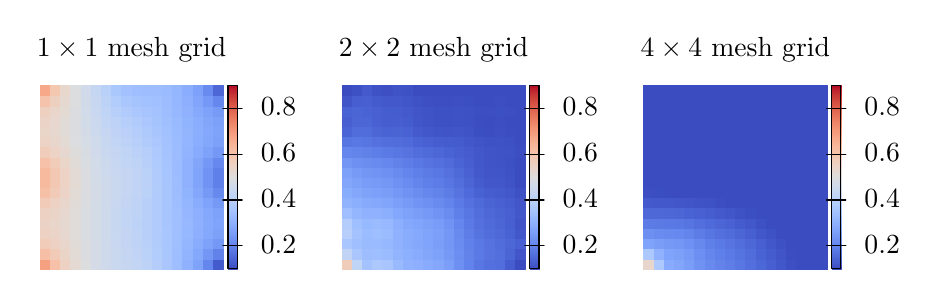
\begin{tikzpicture}[gnuplot]
%% generated with GNUPLOT 5.4p2 (Lua 5.4; terminal rev. Jun 2020, script rev. 114)
%% 11/16/21 06:24:41
\path (0.000,0.000) rectangle (10.000,2.500);
\gpfill{rgb color={0.963,0.629,0.508}} (0.000,0.084)--(0.000,0.214)--(0.130,0.214)--(0.130,0.084)--cycle;
\gpfill{rgb color={0.963,0.756,0.659}} (0.130,0.084)--(0.130,0.214)--(0.259,0.214)--(0.259,0.084)--cycle;
\gpfill{rgb color={0.965,0.745,0.644}} (0.000,0.214)--(0.000,0.343)--(0.130,0.343)--(0.130,0.214)--cycle;
\gpfill{rgb color={0.947,0.797,0.721}} (0.130,0.214)--(0.130,0.343)--(0.259,0.343)--(0.259,0.214)--cycle;
\gpfill{rgb color={0.944,0.801,0.727}} (0.000,0.343)--(0.000,0.473)--(0.130,0.473)--(0.130,0.343)--cycle;
\gpfill{rgb color={0.930,0.821,0.763}} (0.130,0.343)--(0.130,0.473)--(0.259,0.473)--(0.259,0.343)--cycle;
\gpfill{rgb color={0.931,0.819,0.759}} (0.000,0.473)--(0.000,0.603)--(0.130,0.603)--(0.130,0.473)--cycle;
\gpfill{rgb color={0.918,0.833,0.786}} (0.130,0.473)--(0.130,0.603)--(0.259,0.603)--(0.259,0.473)--cycle;
\gpfill{rgb color={0.926,0.825,0.770}} (0.000,0.603)--(0.000,0.732)--(0.130,0.732)--(0.130,0.603)--cycle;
\gpfill{rgb color={0.914,0.837,0.793}} (0.130,0.603)--(0.130,0.732)--(0.259,0.732)--(0.259,0.603)--cycle;
\gpfill{rgb color={0.931,0.820,0.760}} (0.000,0.732)--(0.000,0.862)--(0.130,0.862)--(0.130,0.732)--cycle;
\gpfill{rgb color={0.919,0.833,0.785}} (0.130,0.732)--(0.130,0.862)--(0.259,0.862)--(0.259,0.732)--cycle;
\gpfill{rgb color={0.946,0.798,0.721}} (0.000,0.862)--(0.000,0.991)--(0.130,0.991)--(0.130,0.862)--cycle;
\gpfill{rgb color={0.930,0.821,0.762}} (0.130,0.862)--(0.130,0.991)--(0.259,0.991)--(0.259,0.862)--cycle;
\gpfill{rgb color={0.964,0.753,0.654}} (0.000,0.991)--(0.000,1.121)--(0.130,1.121)--(0.130,0.991)--cycle;
\gpfill{rgb color={0.947,0.797,0.721}} (0.130,0.991)--(0.130,1.121)--(0.259,1.121)--(0.259,0.991)--cycle;
\gpfill{rgb color={0.968,0.728,0.620}} (0.000,1.121)--(0.000,1.250)--(0.130,1.250)--(0.130,1.121)--cycle;
\gpfill{rgb color={0.953,0.785,0.701}} (0.130,1.121)--(0.130,1.250)--(0.259,1.250)--(0.259,1.121)--cycle;
\gpfill{rgb color={0.968,0.729,0.622}} (0.000,1.250)--(0.000,1.379)--(0.130,1.379)--(0.130,1.250)--cycle;
\gpfill{rgb color={0.952,0.786,0.703}} (0.130,1.250)--(0.130,1.379)--(0.259,1.379)--(0.259,1.250)--cycle;
\gpfill{rgb color={0.963,0.756,0.658}} (0.000,1.379)--(0.000,1.509)--(0.130,1.509)--(0.130,1.379)--cycle;
\gpfill{rgb color={0.945,0.801,0.727}} (0.130,1.379)--(0.130,1.509)--(0.259,1.509)--(0.259,1.379)--cycle;
\gpfill{rgb color={0.943,0.803,0.730}} (0.000,1.509)--(0.000,1.638)--(0.130,1.638)--(0.130,1.509)--cycle;
\gpfill{rgb color={0.926,0.826,0.772}} (0.130,1.509)--(0.130,1.638)--(0.259,1.638)--(0.259,1.509)--cycle;
\gpfill{rgb color={0.925,0.826,0.773}} (0.000,1.638)--(0.000,1.768)--(0.130,1.768)--(0.130,1.638)--cycle;
\gpfill{rgb color={0.910,0.840,0.800}} (0.130,1.638)--(0.130,1.768)--(0.259,1.768)--(0.259,1.638)--cycle;
\gpfill{rgb color={0.917,0.834,0.787}} (0.000,1.768)--(0.000,1.897)--(0.130,1.897)--(0.130,1.768)--cycle;
\gpfill{rgb color={0.903,0.845,0.813}} (0.130,1.768)--(0.130,1.897)--(0.259,1.897)--(0.259,1.768)--cycle;
\gpfill{rgb color={0.921,0.831,0.781}} (0.000,1.897)--(0.000,2.027)--(0.130,2.027)--(0.130,1.897)--cycle;
\gpfill{rgb color={0.905,0.844,0.809}} (0.130,1.897)--(0.130,2.027)--(0.259,2.027)--(0.259,1.897)--cycle;
\gpfill{rgb color={0.934,0.816,0.753}} (0.000,2.027)--(0.000,2.157)--(0.130,2.157)--(0.130,2.027)--cycle;
\gpfill{rgb color={0.916,0.835,0.791}} (0.130,2.027)--(0.130,2.157)--(0.259,2.157)--(0.259,2.027)--cycle;
\gpfill{rgb color={0.960,0.766,0.672}} (0.000,2.157)--(0.000,2.286)--(0.130,2.286)--(0.130,2.157)--cycle;
\gpfill{rgb color={0.934,0.816,0.752}} (0.130,2.157)--(0.130,2.286)--(0.259,2.286)--(0.259,2.157)--cycle;
\gpfill{rgb color={0.968,0.657,0.537}} (0.000,2.286)--(0.000,2.416)--(0.130,2.416)--(0.130,2.286)--cycle;
\gpfill{rgb color={0.955,0.780,0.693}} (0.130,2.286)--(0.130,2.416)--(0.259,2.416)--(0.259,2.286)--cycle;
\gpfill{rgb color={0.928,0.823,0.766}} (0.259,0.084)--(0.259,0.214)--(0.389,0.214)--(0.389,0.084)--cycle;
\gpfill{rgb color={0.893,0.852,0.828}} (0.389,0.084)--(0.389,0.214)--(0.519,0.214)--(0.519,0.084)--cycle;
\gpfill{rgb color={0.919,0.832,0.785}} (0.259,0.214)--(0.259,0.343)--(0.389,0.343)--(0.389,0.214)--cycle;
\gpfill{rgb color={0.888,0.855,0.836}} (0.389,0.214)--(0.389,0.343)--(0.519,0.343)--(0.519,0.214)--cycle;
\gpfill{rgb color={0.910,0.841,0.802}} (0.259,0.343)--(0.259,0.473)--(0.389,0.473)--(0.389,0.343)--cycle;
\gpfill{rgb color={0.882,0.858,0.844}} (0.389,0.343)--(0.389,0.473)--(0.519,0.473)--(0.519,0.343)--cycle;
\gpfill{rgb color={0.901,0.847,0.817}} (0.259,0.473)--(0.259,0.603)--(0.389,0.603)--(0.389,0.473)--cycle;
\gpfill{rgb color={0.876,0.861,0.852}} (0.389,0.473)--(0.389,0.603)--(0.519,0.603)--(0.519,0.473)--cycle;
\gpfill{rgb color={0.897,0.849,0.821}} (0.259,0.603)--(0.259,0.732)--(0.389,0.732)--(0.389,0.603)--cycle;
\gpfill{rgb color={0.874,0.862,0.854}} (0.389,0.603)--(0.389,0.732)--(0.519,0.732)--(0.519,0.603)--cycle;
\gpfill{rgb color={0.901,0.847,0.816}} (0.259,0.732)--(0.259,0.862)--(0.389,0.862)--(0.389,0.732)--cycle;
\gpfill{rgb color={0.876,0.861,0.851}} (0.389,0.732)--(0.389,0.862)--(0.519,0.862)--(0.519,0.732)--cycle;
\gpfill{rgb color={0.909,0.841,0.803}} (0.259,0.862)--(0.259,0.991)--(0.389,0.991)--(0.389,0.862)--cycle;
\gpfill{rgb color={0.881,0.859,0.845}} (0.389,0.862)--(0.389,0.991)--(0.519,0.991)--(0.519,0.862)--cycle;
\gpfill{rgb color={0.921,0.831,0.782}} (0.259,0.991)--(0.259,1.121)--(0.389,1.121)--(0.389,0.991)--cycle;
\gpfill{rgb color={0.888,0.855,0.835}} (0.389,0.991)--(0.389,1.121)--(0.519,1.121)--(0.519,0.991)--cycle;
\gpfill{rgb color={0.925,0.826,0.772}} (0.259,1.121)--(0.259,1.250)--(0.389,1.250)--(0.389,1.121)--cycle;
\gpfill{rgb color={0.891,0.853,0.832}} (0.389,1.121)--(0.389,1.250)--(0.519,1.250)--(0.519,1.121)--cycle;
\gpfill{rgb color={0.924,0.827,0.774}} (0.259,1.250)--(0.259,1.379)--(0.389,1.379)--(0.389,1.250)--cycle;
\gpfill{rgb color={0.889,0.854,0.834}} (0.389,1.250)--(0.389,1.379)--(0.519,1.379)--(0.519,1.250)--cycle;
\gpfill{rgb color={0.917,0.834,0.788}} (0.259,1.379)--(0.259,1.509)--(0.389,1.509)--(0.389,1.379)--cycle;
\gpfill{rgb color={0.883,0.858,0.843}} (0.389,1.379)--(0.389,1.509)--(0.519,1.509)--(0.519,1.379)--cycle;
\gpfill{rgb color={0.902,0.846,0.814}} (0.259,1.509)--(0.259,1.638)--(0.389,1.638)--(0.389,1.509)--cycle;
\gpfill{rgb color={0.871,0.863,0.858}} (0.389,1.509)--(0.389,1.638)--(0.519,1.638)--(0.519,1.509)--cycle;
\gpfill{rgb color={0.890,0.854,0.833}} (0.259,1.638)--(0.259,1.768)--(0.389,1.768)--(0.389,1.638)--cycle;
\gpfill{rgb color={0.862,0.865,0.869}} (0.389,1.638)--(0.389,1.768)--(0.519,1.768)--(0.519,1.638)--cycle;
\gpfill{rgb color={0.883,0.858,0.843}} (0.259,1.768)--(0.259,1.897)--(0.389,1.897)--(0.389,1.768)--cycle;
\gpfill{rgb color={0.856,0.864,0.876}} (0.389,1.768)--(0.389,1.897)--(0.519,1.897)--(0.519,1.768)--cycle;
\gpfill{rgb color={0.882,0.858,0.843}} (0.259,1.897)--(0.259,2.027)--(0.389,2.027)--(0.389,1.897)--cycle;
\gpfill{rgb color={0.854,0.864,0.879}} (0.389,1.897)--(0.389,2.027)--(0.519,2.027)--(0.519,1.897)--cycle;
\gpfill{rgb color={0.890,0.854,0.833}} (0.259,2.027)--(0.259,2.157)--(0.389,2.157)--(0.389,2.027)--cycle;
\gpfill{rgb color={0.855,0.864,0.878}} (0.389,2.027)--(0.389,2.157)--(0.519,2.157)--(0.519,2.027)--cycle;
\gpfill{rgb color={0.898,0.849,0.820}} (0.259,2.157)--(0.259,2.286)--(0.389,2.286)--(0.389,2.157)--cycle;
\gpfill{rgb color={0.858,0.865,0.875}} (0.389,2.157)--(0.389,2.286)--(0.519,2.286)--(0.519,2.157)--cycle;
\gpfill{rgb color={0.908,0.842,0.804}} (0.259,2.286)--(0.259,2.416)--(0.389,2.416)--(0.389,2.286)--cycle;
\gpfill{rgb color={0.861,0.865,0.871}} (0.389,2.286)--(0.389,2.416)--(0.519,2.416)--(0.519,2.286)--cycle;
\gpfill{rgb color={0.858,0.865,0.874}} (0.519,0.084)--(0.519,0.214)--(0.648,0.214)--(0.648,0.084)--cycle;
\gpfill{rgb color={0.831,0.860,0.903}} (0.648,0.084)--(0.648,0.214)--(0.778,0.214)--(0.778,0.084)--cycle;
\gpfill{rgb color={0.857,0.864,0.876}} (0.519,0.214)--(0.519,0.343)--(0.648,0.343)--(0.648,0.214)--cycle;
\gpfill{rgb color={0.831,0.860,0.903}} (0.648,0.214)--(0.648,0.343)--(0.778,0.343)--(0.778,0.214)--cycle;
\gpfill{rgb color={0.855,0.864,0.878}} (0.519,0.343)--(0.519,0.473)--(0.648,0.473)--(0.648,0.343)--cycle;
\gpfill{rgb color={0.830,0.859,0.904}} (0.648,0.343)--(0.648,0.473)--(0.778,0.473)--(0.778,0.343)--cycle;
\gpfill{rgb color={0.852,0.864,0.881}} (0.519,0.473)--(0.519,0.603)--(0.648,0.603)--(0.648,0.473)--cycle;
\gpfill{rgb color={0.829,0.859,0.905}} (0.648,0.473)--(0.648,0.603)--(0.778,0.603)--(0.778,0.473)--cycle;
\gpfill{rgb color={0.851,0.864,0.882}} (0.519,0.603)--(0.519,0.732)--(0.648,0.732)--(0.648,0.603)--cycle;
\gpfill{rgb color={0.829,0.859,0.906}} (0.648,0.603)--(0.648,0.732)--(0.778,0.732)--(0.778,0.603)--cycle;
\gpfill{rgb color={0.852,0.864,0.881}} (0.519,0.732)--(0.519,0.862)--(0.648,0.862)--(0.648,0.732)--cycle;
\gpfill{rgb color={0.829,0.859,0.906}} (0.648,0.732)--(0.648,0.862)--(0.778,0.862)--(0.778,0.732)--cycle;
\gpfill{rgb color={0.854,0.864,0.880}} (0.519,0.862)--(0.519,0.991)--(0.648,0.991)--(0.648,0.862)--cycle;
\gpfill{rgb color={0.829,0.859,0.905}} (0.648,0.862)--(0.648,0.991)--(0.778,0.991)--(0.778,0.862)--cycle;
\gpfill{rgb color={0.856,0.864,0.877}} (0.519,0.991)--(0.519,1.121)--(0.648,1.121)--(0.648,0.991)--cycle;
\gpfill{rgb color={0.830,0.859,0.905}} (0.648,0.991)--(0.648,1.121)--(0.778,1.121)--(0.778,0.991)--cycle;
\gpfill{rgb color={0.856,0.864,0.877}} (0.519,1.121)--(0.519,1.250)--(0.648,1.250)--(0.648,1.121)--cycle;
\gpfill{rgb color={0.829,0.859,0.906}} (0.648,1.121)--(0.648,1.250)--(0.778,1.250)--(0.778,1.121)--cycle;
\gpfill{rgb color={0.854,0.864,0.879}} (0.519,1.250)--(0.519,1.379)--(0.648,1.379)--(0.648,1.250)--cycle;
\gpfill{rgb color={0.827,0.859,0.908}} (0.648,1.250)--(0.648,1.379)--(0.778,1.379)--(0.778,1.250)--cycle;
\gpfill{rgb color={0.850,0.863,0.884}} (0.519,1.379)--(0.519,1.509)--(0.648,1.509)--(0.648,1.379)--cycle;
\gpfill{rgb color={0.823,0.857,0.911}} (0.648,1.379)--(0.648,1.509)--(0.778,1.509)--(0.778,1.379)--cycle;
\gpfill{rgb color={0.843,0.862,0.891}} (0.519,1.509)--(0.519,1.638)--(0.648,1.638)--(0.648,1.509)--cycle;
\gpfill{rgb color={0.817,0.856,0.917}} (0.648,1.509)--(0.648,1.638)--(0.778,1.638)--(0.778,1.509)--cycle;
\gpfill{rgb color={0.837,0.861,0.898}} (0.519,1.638)--(0.519,1.768)--(0.648,1.768)--(0.648,1.638)--cycle;
\gpfill{rgb color={0.810,0.854,0.922}} (0.648,1.638)--(0.648,1.768)--(0.778,1.768)--(0.778,1.638)--cycle;
\gpfill{rgb color={0.830,0.859,0.904}} (0.519,1.768)--(0.519,1.897)--(0.648,1.897)--(0.648,1.768)--cycle;
\gpfill{rgb color={0.803,0.851,0.928}} (0.648,1.768)--(0.648,1.897)--(0.778,1.897)--(0.778,1.768)--cycle;
\gpfill{rgb color={0.825,0.858,0.909}} (0.519,1.897)--(0.519,2.027)--(0.648,2.027)--(0.648,1.897)--cycle;
\gpfill{rgb color={0.795,0.848,0.934}} (0.648,1.897)--(0.648,2.027)--(0.778,2.027)--(0.778,1.897)--cycle;
\gpfill{rgb color={0.822,0.857,0.912}} (0.519,2.027)--(0.519,2.157)--(0.648,2.157)--(0.648,2.027)--cycle;
\gpfill{rgb color={0.787,0.845,0.940}} (0.648,2.027)--(0.648,2.157)--(0.778,2.157)--(0.778,2.027)--cycle;
\gpfill{rgb color={0.819,0.856,0.915}} (0.519,2.157)--(0.519,2.286)--(0.648,2.286)--(0.648,2.157)--cycle;
\gpfill{rgb color={0.780,0.843,0.945}} (0.648,2.157)--(0.648,2.286)--(0.778,2.286)--(0.778,2.157)--cycle;
\gpfill{rgb color={0.816,0.856,0.917}} (0.519,2.286)--(0.519,2.416)--(0.648,2.416)--(0.648,2.286)--cycle;
\gpfill{rgb color={0.774,0.840,0.949}} (0.648,2.286)--(0.648,2.416)--(0.778,2.416)--(0.778,2.286)--cycle;
\gpfill{rgb color={0.809,0.853,0.923}} (0.778,0.084)--(0.778,0.214)--(0.907,0.214)--(0.907,0.084)--cycle;
\gpfill{rgb color={0.792,0.847,0.937}} (0.907,0.084)--(0.907,0.214)--(1.037,0.214)--(1.037,0.084)--cycle;
\gpfill{rgb color={0.808,0.853,0.924}} (0.778,0.214)--(0.778,0.343)--(0.907,0.343)--(0.907,0.214)--cycle;
\gpfill{rgb color={0.790,0.846,0.938}} (0.907,0.214)--(0.907,0.343)--(1.037,0.343)--(1.037,0.214)--cycle;
\gpfill{rgb color={0.808,0.853,0.924}} (0.778,0.343)--(0.778,0.473)--(0.907,0.473)--(0.907,0.343)--cycle;
\gpfill{rgb color={0.788,0.846,0.940}} (0.907,0.343)--(0.907,0.473)--(1.037,0.473)--(1.037,0.343)--cycle;
\gpfill{rgb color={0.807,0.853,0.925}} (0.778,0.473)--(0.778,0.603)--(0.907,0.603)--(0.907,0.473)--cycle;
\gpfill{rgb color={0.786,0.845,0.941}} (0.907,0.473)--(0.907,0.603)--(1.037,0.603)--(1.037,0.473)--cycle;
\gpfill{rgb color={0.807,0.853,0.925}} (0.778,0.603)--(0.778,0.732)--(0.907,0.732)--(0.907,0.603)--cycle;
\gpfill{rgb color={0.786,0.845,0.941}} (0.907,0.603)--(0.907,0.732)--(1.037,0.732)--(1.037,0.603)--cycle;
\gpfill{rgb color={0.807,0.853,0.925}} (0.778,0.732)--(0.778,0.862)--(0.907,0.862)--(0.907,0.732)--cycle;
\gpfill{rgb color={0.786,0.845,0.941}} (0.907,0.732)--(0.907,0.862)--(1.037,0.862)--(1.037,0.732)--cycle;
\gpfill{rgb color={0.807,0.853,0.925}} (0.778,0.862)--(0.778,0.991)--(0.907,0.991)--(0.907,0.862)--cycle;
\gpfill{rgb color={0.787,0.845,0.940}} (0.907,0.862)--(0.907,0.991)--(1.037,0.991)--(1.037,0.862)--cycle;
\gpfill{rgb color={0.807,0.853,0.925}} (0.778,0.991)--(0.778,1.121)--(0.907,1.121)--(0.907,0.991)--cycle;
\gpfill{rgb color={0.790,0.846,0.938}} (0.907,0.991)--(0.907,1.121)--(1.037,1.121)--(1.037,0.991)--cycle;
\gpfill{rgb color={0.807,0.852,0.925}} (0.778,1.121)--(0.778,1.250)--(0.907,1.250)--(0.907,1.121)--cycle;
\gpfill{rgb color={0.790,0.846,0.938}} (0.907,1.121)--(0.907,1.250)--(1.037,1.250)--(1.037,1.121)--cycle;
\gpfill{rgb color={0.804,0.852,0.927}} (0.778,1.250)--(0.778,1.379)--(0.907,1.379)--(0.907,1.250)--cycle;
\gpfill{rgb color={0.788,0.846,0.940}} (0.907,1.250)--(0.907,1.379)--(1.037,1.379)--(1.037,1.250)--cycle;
\gpfill{rgb color={0.800,0.850,0.931}} (0.778,1.379)--(0.778,1.509)--(0.907,1.509)--(0.907,1.379)--cycle;
\gpfill{rgb color={0.782,0.843,0.944}} (0.907,1.379)--(0.907,1.509)--(1.037,1.509)--(1.037,1.379)--cycle;
\gpfill{rgb color={0.793,0.848,0.936}} (0.778,1.509)--(0.778,1.638)--(0.907,1.638)--(0.907,1.509)--cycle;
\gpfill{rgb color={0.773,0.839,0.950}} (0.907,1.509)--(0.907,1.638)--(1.037,1.638)--(1.037,1.509)--cycle;
\gpfill{rgb color={0.785,0.845,0.942}} (0.778,1.638)--(0.778,1.768)--(0.907,1.768)--(0.907,1.638)--cycle;
\gpfill{rgb color={0.763,0.835,0.956}} (0.907,1.638)--(0.907,1.768)--(1.037,1.768)--(1.037,1.638)--cycle;
\gpfill{rgb color={0.776,0.841,0.948}} (0.778,1.768)--(0.778,1.897)--(0.907,1.897)--(0.907,1.768)--cycle;
\gpfill{rgb color={0.751,0.829,0.963}} (0.907,1.768)--(0.907,1.897)--(1.037,1.897)--(1.037,1.768)--cycle;
\gpfill{rgb color={0.765,0.836,0.955}} (0.778,1.897)--(0.778,2.027)--(0.907,2.027)--(0.907,1.897)--cycle;
\gpfill{rgb color={0.737,0.822,0.970}} (0.907,1.897)--(0.907,2.027)--(1.037,2.027)--(1.037,1.897)--cycle;
\gpfill{rgb color={0.753,0.830,0.962}} (0.778,2.027)--(0.778,2.157)--(0.907,2.157)--(0.907,2.027)--cycle;
\gpfill{rgb color={0.719,0.812,0.978}} (0.907,2.027)--(0.907,2.157)--(1.037,2.157)--(1.037,2.027)--cycle;
\gpfill{rgb color={0.739,0.823,0.969}} (0.778,2.157)--(0.778,2.286)--(0.907,2.286)--(0.907,2.157)--cycle;
\gpfill{rgb color={0.697,0.799,0.986}} (0.907,2.157)--(0.907,2.286)--(1.037,2.286)--(1.037,2.157)--cycle;
\gpfill{rgb color={0.726,0.816,0.975}} (0.778,2.286)--(0.778,2.416)--(0.907,2.416)--(0.907,2.286)--cycle;
\gpfill{rgb color={0.672,0.783,0.993}} (0.907,2.286)--(0.907,2.416)--(1.037,2.416)--(1.037,2.286)--cycle;
\gpfill{rgb color={0.777,0.841,0.947}} (1.037,0.084)--(1.037,0.214)--(1.166,0.214)--(1.166,0.084)--cycle;
\gpfill{rgb color={0.763,0.835,0.956}} (1.166,0.084)--(1.166,0.214)--(1.295,0.214)--(1.295,0.084)--cycle;
\gpfill{rgb color={0.772,0.839,0.950}} (1.037,0.214)--(1.037,0.343)--(1.166,0.343)--(1.166,0.214)--cycle;
\gpfill{rgb color={0.755,0.831,0.961}} (1.166,0.214)--(1.166,0.343)--(1.295,0.343)--(1.295,0.214)--cycle;
\gpfill{rgb color={0.768,0.837,0.953}} (1.037,0.343)--(1.037,0.473)--(1.166,0.473)--(1.166,0.343)--cycle;
\gpfill{rgb color={0.749,0.828,0.964}} (1.166,0.343)--(1.166,0.473)--(1.295,0.473)--(1.295,0.343)--cycle;
\gpfill{rgb color={0.766,0.836,0.954}} (1.037,0.473)--(1.037,0.603)--(1.166,0.603)--(1.166,0.473)--cycle;
\gpfill{rgb color={0.745,0.826,0.966}} (1.166,0.473)--(1.166,0.603)--(1.295,0.603)--(1.295,0.473)--cycle;
\gpfill{rgb color={0.765,0.836,0.955}} (1.037,0.603)--(1.037,0.732)--(1.166,0.732)--(1.166,0.603)--cycle;
\gpfill{rgb color={0.743,0.825,0.967}} (1.166,0.603)--(1.166,0.732)--(1.295,0.732)--(1.295,0.603)--cycle;
\gpfill{rgb color={0.765,0.836,0.955}} (1.037,0.732)--(1.037,0.862)--(1.166,0.862)--(1.166,0.732)--cycle;
\gpfill{rgb color={0.744,0.826,0.966}} (1.166,0.732)--(1.166,0.862)--(1.295,0.862)--(1.295,0.732)--cycle;
\gpfill{rgb color={0.768,0.837,0.953}} (1.037,0.862)--(1.037,0.991)--(1.166,0.991)--(1.166,0.862)--cycle;
\gpfill{rgb color={0.748,0.828,0.964}} (1.166,0.862)--(1.166,0.991)--(1.295,0.991)--(1.295,0.862)--cycle;
\gpfill{rgb color={0.772,0.839,0.950}} (1.037,0.991)--(1.037,1.121)--(1.166,1.121)--(1.166,0.991)--cycle;
\gpfill{rgb color={0.755,0.831,0.960}} (1.166,0.991)--(1.166,1.121)--(1.295,1.121)--(1.295,0.991)--cycle;
\gpfill{rgb color={0.774,0.840,0.949}} (1.037,1.121)--(1.037,1.250)--(1.166,1.250)--(1.166,1.121)--cycle;
\gpfill{rgb color={0.758,0.833,0.959}} (1.166,1.121)--(1.166,1.250)--(1.295,1.250)--(1.295,1.121)--cycle;
\gpfill{rgb color={0.772,0.839,0.951}} (1.037,1.250)--(1.037,1.379)--(1.166,1.379)--(1.166,1.250)--cycle;
\gpfill{rgb color={0.756,0.832,0.960}} (1.166,1.250)--(1.166,1.379)--(1.295,1.379)--(1.295,1.250)--cycle;
\gpfill{rgb color={0.765,0.836,0.955}} (1.037,1.379)--(1.037,1.509)--(1.166,1.509)--(1.166,1.379)--cycle;
\gpfill{rgb color={0.748,0.828,0.965}} (1.166,1.379)--(1.166,1.509)--(1.295,1.509)--(1.295,1.379)--cycle;
\gpfill{rgb color={0.753,0.830,0.962}} (1.037,1.509)--(1.037,1.638)--(1.166,1.638)--(1.166,1.509)--cycle;
\gpfill{rgb color={0.733,0.820,0.972}} (1.166,1.509)--(1.166,1.638)--(1.295,1.638)--(1.295,1.509)--cycle;
\gpfill{rgb color={0.740,0.824,0.968}} (1.037,1.638)--(1.037,1.768)--(1.166,1.768)--(1.166,1.638)--cycle;
\gpfill{rgb color={0.719,0.812,0.978}} (1.166,1.638)--(1.166,1.768)--(1.295,1.768)--(1.295,1.638)--cycle;
\gpfill{rgb color={0.728,0.817,0.974}} (1.037,1.768)--(1.037,1.897)--(1.166,1.897)--(1.166,1.768)--cycle;
\gpfill{rgb color={0.706,0.805,0.983}} (1.166,1.768)--(1.166,1.897)--(1.295,1.897)--(1.295,1.768)--cycle;
\gpfill{rgb color={0.711,0.808,0.981}} (1.037,1.897)--(1.037,2.027)--(1.166,2.027)--(1.166,1.897)--cycle;
\gpfill{rgb color={0.690,0.795,0.988}} (1.166,1.897)--(1.166,2.027)--(1.295,2.027)--(1.295,1.897)--cycle;
\gpfill{rgb color={0.691,0.795,0.988}} (1.037,2.027)--(1.037,2.157)--(1.166,2.157)--(1.166,2.027)--cycle;
\gpfill{rgb color={0.671,0.782,0.993}} (1.166,2.027)--(1.166,2.157)--(1.295,2.157)--(1.295,2.027)--cycle;
\gpfill{rgb color={0.667,0.779,0.994}} (1.037,2.157)--(1.037,2.286)--(1.166,2.286)--(1.166,2.157)--cycle;
\gpfill{rgb color={0.649,0.767,0.997}} (1.166,2.157)--(1.166,2.286)--(1.295,2.286)--(1.295,2.157)--cycle;
\gpfill{rgb color={0.637,0.758,0.998}} (1.037,2.286)--(1.037,2.416)--(1.166,2.416)--(1.166,2.286)--cycle;
\gpfill{rgb color={0.623,0.747,1.000}} (1.166,2.286)--(1.166,2.416)--(1.295,2.416)--(1.295,2.286)--cycle;
\gpfill{rgb color={0.739,0.823,0.969}} (1.295,0.084)--(1.295,0.214)--(1.425,0.214)--(1.425,0.084)--cycle;
\gpfill{rgb color={0.704,0.803,0.983}} (1.425,0.084)--(1.425,0.214)--(1.554,0.214)--(1.554,0.084)--cycle;
\gpfill{rgb color={0.731,0.819,0.973}} (1.295,0.214)--(1.295,0.343)--(1.425,0.343)--(1.425,0.214)--cycle;
\gpfill{rgb color={0.700,0.801,0.985}} (1.425,0.214)--(1.425,0.343)--(1.554,0.343)--(1.554,0.214)--cycle;
\gpfill{rgb color={0.725,0.816,0.975}} (1.295,0.343)--(1.295,0.473)--(1.425,0.473)--(1.425,0.343)--cycle;
\gpfill{rgb color={0.696,0.798,0.986}} (1.425,0.343)--(1.425,0.473)--(1.554,0.473)--(1.554,0.343)--cycle;
\gpfill{rgb color={0.721,0.813,0.977}} (1.295,0.473)--(1.295,0.603)--(1.425,0.603)--(1.425,0.473)--cycle;
\gpfill{rgb color={0.693,0.796,0.987}} (1.425,0.473)--(1.425,0.603)--(1.554,0.603)--(1.554,0.473)--cycle;
\gpfill{rgb color={0.719,0.812,0.978}} (1.295,0.603)--(1.295,0.732)--(1.425,0.732)--(1.425,0.603)--cycle;
\gpfill{rgb color={0.691,0.795,0.988}} (1.425,0.603)--(1.425,0.732)--(1.554,0.732)--(1.554,0.603)--cycle;
\gpfill{rgb color={0.720,0.812,0.978}} (1.295,0.732)--(1.295,0.862)--(1.425,0.862)--(1.425,0.732)--cycle;
\gpfill{rgb color={0.691,0.795,0.988}} (1.425,0.732)--(1.425,0.862)--(1.554,0.862)--(1.554,0.732)--cycle;
\gpfill{rgb color={0.723,0.815,0.976}} (1.295,0.862)--(1.295,0.991)--(1.425,0.991)--(1.425,0.862)--cycle;
\gpfill{rgb color={0.693,0.796,0.987}} (1.425,0.862)--(1.425,0.991)--(1.554,0.991)--(1.554,0.862)--cycle;
\gpfill{rgb color={0.730,0.818,0.973}} (1.295,0.991)--(1.295,1.121)--(1.425,1.121)--(1.425,0.991)--cycle;
\gpfill{rgb color={0.696,0.798,0.986}} (1.425,0.991)--(1.425,1.121)--(1.554,1.121)--(1.554,0.991)--cycle;
\gpfill{rgb color={0.732,0.820,0.972}} (1.295,1.121)--(1.295,1.250)--(1.425,1.250)--(1.425,1.121)--cycle;
\gpfill{rgb color={0.696,0.799,0.986}} (1.425,1.121)--(1.425,1.250)--(1.554,1.250)--(1.554,1.121)--cycle;
\gpfill{rgb color={0.730,0.818,0.973}} (1.295,1.250)--(1.295,1.379)--(1.425,1.379)--(1.425,1.250)--cycle;
\gpfill{rgb color={0.694,0.797,0.987}} (1.425,1.250)--(1.425,1.379)--(1.554,1.379)--(1.554,1.250)--cycle;
\gpfill{rgb color={0.722,0.814,0.977}} (1.295,1.379)--(1.295,1.509)--(1.425,1.509)--(1.425,1.379)--cycle;
\gpfill{rgb color={0.688,0.793,0.988}} (1.425,1.379)--(1.425,1.509)--(1.554,1.509)--(1.554,1.379)--cycle;
\gpfill{rgb color={0.708,0.806,0.982}} (1.295,1.509)--(1.295,1.638)--(1.425,1.638)--(1.425,1.509)--cycle;
\gpfill{rgb color={0.679,0.787,0.991}} (1.425,1.509)--(1.425,1.638)--(1.554,1.638)--(1.554,1.509)--cycle;
\gpfill{rgb color={0.695,0.798,0.986}} (1.295,1.638)--(1.295,1.768)--(1.425,1.768)--(1.425,1.638)--cycle;
\gpfill{rgb color={0.669,0.781,0.993}} (1.425,1.638)--(1.425,1.768)--(1.554,1.768)--(1.554,1.638)--cycle;
\gpfill{rgb color={0.683,0.790,0.990}} (1.295,1.768)--(1.295,1.897)--(1.425,1.897)--(1.425,1.768)--cycle;
\gpfill{rgb color={0.660,0.774,0.995}} (1.425,1.768)--(1.425,1.897)--(1.554,1.897)--(1.554,1.768)--cycle;
\gpfill{rgb color={0.669,0.781,0.993}} (1.295,1.897)--(1.295,2.027)--(1.425,2.027)--(1.425,1.897)--cycle;
\gpfill{rgb color={0.649,0.767,0.997}} (1.425,1.897)--(1.425,2.027)--(1.554,2.027)--(1.554,1.897)--cycle;
\gpfill{rgb color={0.653,0.770,0.996}} (1.295,2.027)--(1.295,2.157)--(1.425,2.157)--(1.425,2.027)--cycle;
\gpfill{rgb color={0.638,0.759,0.998}} (1.425,2.027)--(1.425,2.157)--(1.554,2.157)--(1.554,2.027)--cycle;
\gpfill{rgb color={0.636,0.757,0.999}} (1.295,2.157)--(1.295,2.286)--(1.425,2.286)--(1.425,2.157)--cycle;
\gpfill{rgb color={0.627,0.751,0.999}} (1.425,2.157)--(1.425,2.286)--(1.554,2.286)--(1.554,2.157)--cycle;
\gpfill{rgb color={0.616,0.742,1.000}} (1.295,2.286)--(1.295,2.416)--(1.425,2.416)--(1.425,2.286)--cycle;
\gpfill{rgb color={0.617,0.743,1.000}} (1.425,2.286)--(1.425,2.416)--(1.554,2.416)--(1.554,2.286)--cycle;
\gpfill{rgb color={0.665,0.778,0.994}} (1.554,0.084)--(1.554,0.214)--(1.684,0.214)--(1.684,0.084)--cycle;
\gpfill{rgb color={0.621,0.745,1.000}} (1.684,0.084)--(1.684,0.214)--(1.813,0.214)--(1.813,0.084)--cycle;
\gpfill{rgb color={0.663,0.777,0.994}} (1.554,0.214)--(1.554,0.343)--(1.684,0.343)--(1.684,0.214)--cycle;
\gpfill{rgb color={0.622,0.747,1.000}} (1.684,0.214)--(1.684,0.343)--(1.813,0.343)--(1.813,0.214)--cycle;
\gpfill{rgb color={0.662,0.776,0.995}} (1.554,0.343)--(1.554,0.473)--(1.684,0.473)--(1.684,0.343)--cycle;
\gpfill{rgb color={0.624,0.748,0.999}} (1.684,0.343)--(1.684,0.473)--(1.813,0.473)--(1.813,0.343)--cycle;
\gpfill{rgb color={0.661,0.775,0.995}} (1.554,0.473)--(1.554,0.603)--(1.684,0.603)--(1.684,0.473)--cycle;
\gpfill{rgb color={0.626,0.750,0.999}} (1.684,0.473)--(1.684,0.603)--(1.813,0.603)--(1.813,0.473)--cycle;
\gpfill{rgb color={0.660,0.775,0.995}} (1.554,0.603)--(1.554,0.732)--(1.684,0.732)--(1.684,0.603)--cycle;
\gpfill{rgb color={0.626,0.750,0.999}} (1.684,0.603)--(1.684,0.732)--(1.813,0.732)--(1.813,0.603)--cycle;
\gpfill{rgb color={0.660,0.774,0.995}} (1.554,0.732)--(1.554,0.862)--(1.684,0.862)--(1.684,0.732)--cycle;
\gpfill{rgb color={0.624,0.749,0.999}} (1.684,0.732)--(1.684,0.862)--(1.813,0.862)--(1.813,0.732)--cycle;
\gpfill{rgb color={0.659,0.774,0.995}} (1.554,0.862)--(1.554,0.991)--(1.684,0.991)--(1.684,0.862)--cycle;
\gpfill{rgb color={0.622,0.746,1.000}} (1.684,0.862)--(1.684,0.991)--(1.813,0.991)--(1.813,0.862)--cycle;
\gpfill{rgb color={0.659,0.774,0.995}} (1.554,0.991)--(1.554,1.121)--(1.684,1.121)--(1.684,0.991)--cycle;
\gpfill{rgb color={0.618,0.743,1.000}} (1.684,0.991)--(1.684,1.121)--(1.813,1.121)--(1.813,0.991)--cycle;
\gpfill{rgb color={0.657,0.773,0.996}} (1.554,1.121)--(1.554,1.250)--(1.684,1.250)--(1.684,1.121)--cycle;
\gpfill{rgb color={0.615,0.741,1.000}} (1.684,1.121)--(1.684,1.250)--(1.813,1.250)--(1.813,1.121)--cycle;
\gpfill{rgb color={0.655,0.771,0.996}} (1.554,1.250)--(1.554,1.379)--(1.684,1.379)--(1.684,1.250)--cycle;
\gpfill{rgb color={0.613,0.739,1.000}} (1.684,1.250)--(1.684,1.379)--(1.813,1.379)--(1.813,1.250)--cycle;
\gpfill{rgb color={0.651,0.768,0.997}} (1.554,1.379)--(1.554,1.509)--(1.684,1.509)--(1.684,1.379)--cycle;
\gpfill{rgb color={0.611,0.738,1.000}} (1.684,1.379)--(1.684,1.509)--(1.813,1.509)--(1.813,1.379)--cycle;
\gpfill{rgb color={0.646,0.765,0.997}} (1.554,1.509)--(1.554,1.638)--(1.684,1.638)--(1.684,1.509)--cycle;
\gpfill{rgb color={0.611,0.738,1.000}} (1.684,1.509)--(1.684,1.638)--(1.813,1.638)--(1.813,1.509)--cycle;
\gpfill{rgb color={0.640,0.761,0.998}} (1.554,1.638)--(1.554,1.768)--(1.684,1.768)--(1.684,1.638)--cycle;
\gpfill{rgb color={0.609,0.736,1.000}} (1.684,1.638)--(1.684,1.768)--(1.813,1.768)--(1.813,1.638)--cycle;
\gpfill{rgb color={0.634,0.755,0.999}} (1.554,1.768)--(1.554,1.897)--(1.684,1.897)--(1.684,1.768)--cycle;
\gpfill{rgb color={0.605,0.733,1.000}} (1.684,1.768)--(1.684,1.897)--(1.813,1.897)--(1.813,1.768)--cycle;
\gpfill{rgb color={0.626,0.750,0.999}} (1.554,1.897)--(1.554,2.027)--(1.684,2.027)--(1.684,1.897)--cycle;
\gpfill{rgb color={0.599,0.728,1.000}} (1.684,1.897)--(1.684,2.027)--(1.813,2.027)--(1.813,1.897)--cycle;
\gpfill{rgb color={0.617,0.743,1.000}} (1.554,2.027)--(1.554,2.157)--(1.684,2.157)--(1.684,2.027)--cycle;
\gpfill{rgb color={0.591,0.722,1.000}} (1.684,2.027)--(1.684,2.157)--(1.813,2.157)--(1.813,2.027)--cycle;
\gpfill{rgb color={0.610,0.737,1.000}} (1.554,2.157)--(1.554,2.286)--(1.684,2.286)--(1.684,2.157)--cycle;
\gpfill{rgb color={0.584,0.716,0.999}} (1.684,2.157)--(1.684,2.286)--(1.813,2.286)--(1.813,2.157)--cycle;
\gpfill{rgb color={0.605,0.733,1.000}} (1.554,2.286)--(1.554,2.416)--(1.684,2.416)--(1.684,2.286)--cycle;
\gpfill{rgb color={0.579,0.712,0.999}} (1.684,2.286)--(1.684,2.416)--(1.813,2.416)--(1.813,2.286)--cycle;
\gpfill{rgb color={0.566,0.700,0.997}} (1.813,0.084)--(1.813,0.214)--(1.943,0.214)--(1.943,0.084)--cycle;
\gpfill{rgb color={0.501,0.639,0.982}} (1.943,0.084)--(1.943,0.214)--(2.073,0.214)--(2.073,0.084)--cycle;
\gpfill{rgb color={0.574,0.707,0.998}} (1.813,0.214)--(1.813,0.343)--(1.943,0.343)--(1.943,0.214)--cycle;
\gpfill{rgb color={0.519,0.658,0.988}} (1.943,0.214)--(1.943,0.343)--(2.073,0.343)--(2.073,0.214)--cycle;
\gpfill{rgb color={0.582,0.714,0.999}} (1.813,0.343)--(1.813,0.473)--(1.943,0.473)--(1.943,0.343)--cycle;
\gpfill{rgb color={0.536,0.673,0.992}} (1.943,0.343)--(1.943,0.473)--(2.073,0.473)--(2.073,0.343)--cycle;
\gpfill{rgb color={0.589,0.720,1.000}} (1.813,0.473)--(1.813,0.603)--(1.943,0.603)--(1.943,0.473)--cycle;
\gpfill{rgb color={0.551,0.687,0.995}} (1.943,0.473)--(1.943,0.603)--(2.073,0.603)--(2.073,0.473)--cycle;
\gpfill{rgb color={0.591,0.722,1.000}} (1.813,0.603)--(1.813,0.732)--(1.943,0.732)--(1.943,0.603)--cycle;
\gpfill{rgb color={0.556,0.691,0.996}} (1.943,0.603)--(1.943,0.732)--(2.073,0.732)--(2.073,0.603)--cycle;
\gpfill{rgb color={0.588,0.719,0.999}} (1.813,0.732)--(1.813,0.862)--(1.943,0.862)--(1.943,0.732)--cycle;
\gpfill{rgb color={0.551,0.687,0.995}} (1.943,0.732)--(1.943,0.862)--(2.073,0.862)--(2.073,0.732)--cycle;
\gpfill{rgb color={0.581,0.714,0.999}} (1.813,0.862)--(1.813,0.991)--(1.943,0.991)--(1.943,0.862)--cycle;
\gpfill{rgb color={0.538,0.675,0.992}} (1.943,0.862)--(1.943,0.991)--(2.073,0.991)--(2.073,0.862)--cycle;
\gpfill{rgb color={0.570,0.704,0.998}} (1.813,0.991)--(1.813,1.121)--(1.943,1.121)--(1.943,0.991)--cycle;
\gpfill{rgb color={0.517,0.656,0.987}} (1.943,0.991)--(1.943,1.121)--(2.073,1.121)--(2.073,0.991)--cycle;
\gpfill{rgb color={0.564,0.699,0.997}} (1.813,1.121)--(1.813,1.250)--(1.943,1.250)--(1.943,1.121)--cycle;
\gpfill{rgb color={0.506,0.645,0.984}} (1.943,1.121)--(1.943,1.250)--(2.073,1.250)--(2.073,1.121)--cycle;
\gpfill{rgb color={0.563,0.697,0.997}} (1.813,1.250)--(1.813,1.379)--(1.943,1.379)--(1.943,1.250)--cycle;
\gpfill{rgb color={0.505,0.644,0.983}} (1.943,1.250)--(1.943,1.379)--(2.073,1.379)--(2.073,1.250)--cycle;
\gpfill{rgb color={0.565,0.700,0.997}} (1.813,1.379)--(1.813,1.509)--(1.943,1.509)--(1.943,1.379)--cycle;
\gpfill{rgb color={0.514,0.652,0.986}} (1.943,1.379)--(1.943,1.509)--(2.073,1.509)--(2.073,1.379)--cycle;
\gpfill{rgb color={0.573,0.706,0.998}} (1.813,1.509)--(1.813,1.638)--(1.943,1.638)--(1.943,1.509)--cycle;
\gpfill{rgb color={0.532,0.670,0.991}} (1.943,1.509)--(1.943,1.638)--(2.073,1.638)--(2.073,1.509)--cycle;
\gpfill{rgb color={0.576,0.709,0.999}} (1.813,1.638)--(1.813,1.768)--(1.943,1.768)--(1.943,1.638)--cycle;
\gpfill{rgb color={0.542,0.679,0.993}} (1.943,1.638)--(1.943,1.768)--(2.073,1.768)--(2.073,1.638)--cycle;
\gpfill{rgb color={0.576,0.709,0.998}} (1.813,1.768)--(1.813,1.897)--(1.943,1.897)--(1.943,1.768)--cycle;
\gpfill{rgb color={0.545,0.682,0.994}} (1.943,1.768)--(1.943,1.897)--(2.073,1.897)--(2.073,1.768)--cycle;
\gpfill{rgb color={0.570,0.704,0.998}} (1.813,1.897)--(1.813,2.027)--(1.943,2.027)--(1.943,1.897)--cycle;
\gpfill{rgb color={0.540,0.677,0.993}} (1.943,1.897)--(1.943,2.027)--(2.073,2.027)--(2.073,1.897)--cycle;
\gpfill{rgb color={0.560,0.695,0.997}} (1.813,2.027)--(1.813,2.157)--(1.943,2.157)--(1.943,2.027)--cycle;
\gpfill{rgb color={0.525,0.663,0.989}} (1.943,2.027)--(1.943,2.157)--(2.073,2.157)--(2.073,2.027)--cycle;
\gpfill{rgb color={0.551,0.687,0.995}} (1.813,2.157)--(1.813,2.286)--(1.943,2.286)--(1.943,2.157)--cycle;
\gpfill{rgb color={0.509,0.648,0.985}} (1.943,2.157)--(1.943,2.286)--(2.073,2.286)--(2.073,2.157)--cycle;
\gpfill{rgb color={0.542,0.679,0.993}} (1.813,2.286)--(1.813,2.416)--(1.943,2.416)--(1.943,2.286)--cycle;
\gpfill{rgb color={0.492,0.631,0.979}} (1.943,2.286)--(1.943,2.416)--(2.073,2.416)--(2.073,2.286)--cycle;
\gpfill{rgb color={0.398,0.528,0.929}} (2.073,0.084)--(2.073,0.214)--(2.202,0.214)--(2.202,0.084)--cycle;
\gpfill{rgb color={0.268,0.356,0.804}} (2.202,0.084)--(2.202,0.214)--(2.332,0.214)--(2.332,0.084)--cycle;
\gpfill{rgb color={0.455,0.592,0.963}} (2.073,0.214)--(2.073,0.343)--(2.202,0.343)--(2.202,0.214)--cycle;
\gpfill{rgb color={0.384,0.510,0.918}} (2.202,0.214)--(2.202,0.343)--(2.332,0.343)--(2.332,0.214)--cycle;
\gpfill{rgb color={0.496,0.634,0.980}} (2.073,0.343)--(2.073,0.473)--(2.202,0.473)--(2.202,0.343)--cycle;
\gpfill{rgb color={0.460,0.598,0.965}} (2.202,0.343)--(2.202,0.473)--(2.332,0.473)--(2.332,0.343)--cycle;
\gpfill{rgb color={0.518,0.657,0.987}} (2.073,0.473)--(2.073,0.603)--(2.202,0.603)--(2.202,0.473)--cycle;
\gpfill{rgb color={0.491,0.630,0.978}} (2.202,0.473)--(2.202,0.603)--(2.332,0.603)--(2.332,0.473)--cycle;
\gpfill{rgb color={0.526,0.664,0.990}} (2.073,0.603)--(2.073,0.732)--(2.202,0.732)--(2.202,0.603)--cycle;
\gpfill{rgb color={0.503,0.641,0.983}} (2.202,0.603)--(2.202,0.732)--(2.332,0.732)--(2.332,0.603)--cycle;
\gpfill{rgb color={0.520,0.658,0.988}} (2.073,0.732)--(2.073,0.862)--(2.202,0.862)--(2.202,0.732)--cycle;
\gpfill{rgb color={0.494,0.633,0.980}} (2.202,0.732)--(2.202,0.862)--(2.332,0.862)--(2.332,0.732)--cycle;
\gpfill{rgb color={0.498,0.637,0.981}} (2.073,0.862)--(2.073,0.991)--(2.202,0.991)--(2.202,0.862)--cycle;
\gpfill{rgb color={0.461,0.599,0.966}} (2.202,0.862)--(2.202,0.991)--(2.332,0.991)--(2.332,0.862)--cycle;
\gpfill{rgb color={0.462,0.599,0.966}} (2.073,0.991)--(2.073,1.121)--(2.202,1.121)--(2.202,0.991)--cycle;
\gpfill{rgb color={0.405,0.536,0.933}} (2.202,0.991)--(2.202,1.121)--(2.332,1.121)--(2.332,0.991)--cycle;
\gpfill{rgb color={0.444,0.580,0.957}} (2.073,1.121)--(2.073,1.250)--(2.202,1.250)--(2.202,1.121)--cycle;
\gpfill{rgb color={0.377,0.502,0.913}} (2.202,1.121)--(2.202,1.250)--(2.332,1.250)--(2.332,1.121)--cycle;
\gpfill{rgb color={0.443,0.579,0.956}} (2.073,1.250)--(2.073,1.379)--(2.202,1.379)--(2.202,1.250)--cycle;
\gpfill{rgb color={0.377,0.502,0.913}} (2.202,1.250)--(2.202,1.379)--(2.332,1.379)--(2.332,1.250)--cycle;
\gpfill{rgb color={0.460,0.597,0.965}} (2.073,1.379)--(2.073,1.509)--(2.202,1.509)--(2.202,1.379)--cycle;
\gpfill{rgb color={0.404,0.534,0.932}} (2.202,1.379)--(2.202,1.509)--(2.332,1.509)--(2.332,1.379)--cycle;
\gpfill{rgb color={0.494,0.633,0.979}} (2.073,1.509)--(2.073,1.638)--(2.202,1.638)--(2.202,1.509)--cycle;
\gpfill{rgb color={0.459,0.596,0.964}} (2.202,1.509)--(2.202,1.638)--(2.332,1.638)--(2.332,1.509)--cycle;
\gpfill{rgb color={0.514,0.653,0.986}} (2.073,1.638)--(2.073,1.768)--(2.202,1.768)--(2.202,1.638)--cycle;
\gpfill{rgb color={0.491,0.630,0.978}} (2.202,1.638)--(2.202,1.768)--(2.332,1.768)--(2.332,1.638)--cycle;
\gpfill{rgb color={0.520,0.658,0.988}} (2.073,1.768)--(2.073,1.897)--(2.202,1.897)--(2.202,1.768)--cycle;
\gpfill{rgb color={0.500,0.639,0.982}} (2.202,1.768)--(2.202,1.897)--(2.332,1.897)--(2.332,1.768)--cycle;
\gpfill{rgb color={0.513,0.652,0.986}} (2.073,1.897)--(2.073,2.027)--(2.202,2.027)--(2.202,1.897)--cycle;
\gpfill{rgb color={0.491,0.630,0.978}} (2.202,1.897)--(2.202,2.027)--(2.332,2.027)--(2.332,1.897)--cycle;
\gpfill{rgb color={0.493,0.632,0.979}} (2.073,2.027)--(2.073,2.157)--(2.202,2.157)--(2.202,2.027)--cycle;
\gpfill{rgb color={0.465,0.603,0.967}} (2.202,2.027)--(2.202,2.157)--(2.332,2.157)--(2.332,2.027)--cycle;
\gpfill{rgb color={0.459,0.596,0.964}} (2.073,2.157)--(2.073,2.286)--(2.202,2.286)--(2.202,2.157)--cycle;
\gpfill{rgb color={0.400,0.530,0.930}} (2.202,2.157)--(2.202,2.286)--(2.332,2.286)--(2.332,2.157)--cycle;
\gpfill{rgb color={0.411,0.542,0.937}} (2.073,2.286)--(2.073,2.416)--(2.202,2.416)--(2.202,2.286)--cycle;
\gpfill{rgb color={0.302,0.404,0.843}} (2.202,2.286)--(2.202,2.416)--(2.332,2.416)--(2.332,2.286)--cycle;
\gpfill{rgb color={0.230,0.299,0.754}} (2.390,0.084)--(2.506,0.084)--(2.506,0.094)--(2.390,0.094)--cycle;
\gpfill{rgb color={0.235,0.306,0.760}} (2.390,0.093)--(2.506,0.093)--(2.506,0.103)--(2.390,0.103)--cycle;
\gpfill{rgb color={0.239,0.313,0.767}} (2.390,0.102)--(2.506,0.102)--(2.506,0.112)--(2.390,0.112)--cycle;
\gpfill{rgb color={0.244,0.320,0.773}} (2.390,0.111)--(2.506,0.111)--(2.506,0.121)--(2.390,0.121)--cycle;
\gpfill{rgb color={0.248,0.326,0.778}} (2.390,0.120)--(2.506,0.120)--(2.506,0.130)--(2.390,0.130)--cycle;
\gpfill{rgb color={0.253,0.333,0.784}} (2.390,0.129)--(2.506,0.129)--(2.506,0.139)--(2.390,0.139)--cycle;
\gpfill{rgb color={0.257,0.340,0.790}} (2.390,0.138)--(2.506,0.138)--(2.506,0.148)--(2.390,0.148)--cycle;
\gpfill{rgb color={0.262,0.347,0.796}} (2.390,0.147)--(2.506,0.147)--(2.506,0.157)--(2.390,0.157)--cycle;
\gpfill{rgb color={0.266,0.353,0.802}} (2.390,0.156)--(2.506,0.156)--(2.506,0.166)--(2.390,0.166)--cycle;
\gpfill{rgb color={0.271,0.360,0.807}} (2.390,0.165)--(2.506,0.165)--(2.506,0.176)--(2.390,0.176)--cycle;
\gpfill{rgb color={0.276,0.367,0.813}} (2.390,0.175)--(2.506,0.175)--(2.506,0.185)--(2.390,0.185)--cycle;
\gpfill{rgb color={0.281,0.374,0.819}} (2.390,0.184)--(2.506,0.184)--(2.506,0.194)--(2.390,0.194)--cycle;
\gpfill{rgb color={0.285,0.380,0.824}} (2.390,0.193)--(2.506,0.193)--(2.506,0.203)--(2.390,0.203)--cycle;
\gpfill{rgb color={0.290,0.387,0.830}} (2.390,0.202)--(2.506,0.202)--(2.506,0.212)--(2.390,0.212)--cycle;
\gpfill{rgb color={0.295,0.394,0.835}} (2.390,0.211)--(2.506,0.211)--(2.506,0.221)--(2.390,0.221)--cycle;
\gpfill{rgb color={0.299,0.400,0.840}} (2.390,0.220)--(2.506,0.220)--(2.506,0.230)--(2.390,0.230)--cycle;
\gpfill{rgb color={0.304,0.407,0.845}} (2.390,0.229)--(2.506,0.229)--(2.506,0.239)--(2.390,0.239)--cycle;
\gpfill{rgb color={0.309,0.413,0.850}} (2.390,0.238)--(2.506,0.238)--(2.506,0.248)--(2.390,0.248)--cycle;
\gpfill{rgb color={0.313,0.420,0.855}} (2.390,0.247)--(2.506,0.247)--(2.506,0.258)--(2.390,0.258)--cycle;
\gpfill{rgb color={0.319,0.427,0.861}} (2.390,0.257)--(2.506,0.257)--(2.506,0.267)--(2.390,0.267)--cycle;
\gpfill{rgb color={0.324,0.433,0.865}} (2.390,0.266)--(2.506,0.266)--(2.506,0.276)--(2.390,0.276)--cycle;
\gpfill{rgb color={0.328,0.440,0.870}} (2.390,0.275)--(2.506,0.275)--(2.506,0.285)--(2.390,0.285)--cycle;
\gpfill{rgb color={0.333,0.446,0.875}} (2.390,0.284)--(2.506,0.284)--(2.506,0.294)--(2.390,0.294)--cycle;
\gpfill{rgb color={0.338,0.453,0.879}} (2.390,0.293)--(2.506,0.293)--(2.506,0.303)--(2.390,0.303)--cycle;
\gpfill{rgb color={0.343,0.459,0.884}} (2.390,0.302)--(2.506,0.302)--(2.506,0.312)--(2.390,0.312)--cycle;
\gpfill{rgb color={0.348,0.465,0.888}} (2.390,0.311)--(2.506,0.311)--(2.506,0.321)--(2.390,0.321)--cycle;
\gpfill{rgb color={0.353,0.472,0.893}} (2.390,0.320)--(2.506,0.320)--(2.506,0.330)--(2.390,0.330)--cycle;
\gpfill{rgb color={0.358,0.478,0.897}} (2.390,0.329)--(2.506,0.329)--(2.506,0.340)--(2.390,0.340)--cycle;
\gpfill{rgb color={0.363,0.485,0.902}} (2.390,0.339)--(2.506,0.339)--(2.506,0.349)--(2.390,0.349)--cycle;
\gpfill{rgb color={0.368,0.491,0.906}} (2.390,0.348)--(2.506,0.348)--(2.506,0.358)--(2.390,0.358)--cycle;
\gpfill{rgb color={0.373,0.497,0.910}} (2.390,0.357)--(2.506,0.357)--(2.506,0.367)--(2.390,0.367)--cycle;
\gpfill{rgb color={0.378,0.504,0.914}} (2.390,0.366)--(2.506,0.366)--(2.506,0.376)--(2.390,0.376)--cycle;
\gpfill{rgb color={0.383,0.510,0.918}} (2.390,0.375)--(2.506,0.375)--(2.506,0.385)--(2.390,0.385)--cycle;
\gpfill{rgb color={0.388,0.516,0.921}} (2.390,0.384)--(2.506,0.384)--(2.506,0.394)--(2.390,0.394)--cycle;
\gpfill{rgb color={0.393,0.522,0.925}} (2.390,0.393)--(2.506,0.393)--(2.506,0.403)--(2.390,0.403)--cycle;
\gpfill{rgb color={0.398,0.528,0.929}} (2.390,0.402)--(2.506,0.402)--(2.506,0.412)--(2.390,0.412)--cycle;
\gpfill{rgb color={0.404,0.534,0.932}} (2.390,0.411)--(2.506,0.411)--(2.506,0.422)--(2.390,0.422)--cycle;
\gpfill{rgb color={0.409,0.541,0.936}} (2.390,0.421)--(2.506,0.421)--(2.506,0.431)--(2.390,0.431)--cycle;
\gpfill{rgb color={0.414,0.547,0.939}} (2.390,0.430)--(2.506,0.430)--(2.506,0.440)--(2.390,0.440)--cycle;
\gpfill{rgb color={0.420,0.553,0.943}} (2.390,0.439)--(2.506,0.439)--(2.506,0.449)--(2.390,0.449)--cycle;
\gpfill{rgb color={0.425,0.559,0.946}} (2.390,0.448)--(2.506,0.448)--(2.506,0.458)--(2.390,0.458)--cycle;
\gpfill{rgb color={0.430,0.564,0.949}} (2.390,0.457)--(2.506,0.457)--(2.506,0.467)--(2.390,0.467)--cycle;
\gpfill{rgb color={0.435,0.570,0.952}} (2.390,0.466)--(2.506,0.466)--(2.506,0.476)--(2.390,0.476)--cycle;
\gpfill{rgb color={0.440,0.576,0.955}} (2.390,0.475)--(2.506,0.475)--(2.506,0.485)--(2.390,0.485)--cycle;
\gpfill{rgb color={0.446,0.582,0.958}} (2.390,0.484)--(2.506,0.484)--(2.506,0.494)--(2.390,0.494)--cycle;
\gpfill{rgb color={0.451,0.588,0.960}} (2.390,0.493)--(2.506,0.493)--(2.506,0.504)--(2.390,0.504)--cycle;
\gpfill{rgb color={0.457,0.594,0.963}} (2.390,0.503)--(2.506,0.503)--(2.506,0.513)--(2.390,0.513)--cycle;
\gpfill{rgb color={0.462,0.599,0.966}} (2.390,0.512)--(2.506,0.512)--(2.506,0.522)--(2.390,0.522)--cycle;
\gpfill{rgb color={0.467,0.605,0.968}} (2.390,0.521)--(2.506,0.521)--(2.506,0.531)--(2.390,0.531)--cycle;
\gpfill{rgb color={0.472,0.611,0.971}} (2.390,0.530)--(2.506,0.530)--(2.506,0.540)--(2.390,0.540)--cycle;
\gpfill{rgb color={0.478,0.616,0.973}} (2.390,0.539)--(2.506,0.539)--(2.506,0.549)--(2.390,0.549)--cycle;
\gpfill{rgb color={0.483,0.622,0.975}} (2.390,0.548)--(2.506,0.548)--(2.506,0.558)--(2.390,0.558)--cycle;
\gpfill{rgb color={0.488,0.627,0.977}} (2.390,0.557)--(2.506,0.557)--(2.506,0.567)--(2.390,0.567)--cycle;
\gpfill{rgb color={0.494,0.632,0.979}} (2.390,0.566)--(2.506,0.566)--(2.506,0.576)--(2.390,0.576)--cycle;
\gpfill{rgb color={0.499,0.638,0.981}} (2.390,0.575)--(2.506,0.575)--(2.506,0.586)--(2.390,0.586)--cycle;
\gpfill{rgb color={0.505,0.644,0.983}} (2.390,0.585)--(2.506,0.585)--(2.506,0.595)--(2.390,0.595)--cycle;
\gpfill{rgb color={0.510,0.649,0.985}} (2.390,0.594)--(2.506,0.594)--(2.506,0.604)--(2.390,0.604)--cycle;
\gpfill{rgb color={0.515,0.654,0.987}} (2.390,0.603)--(2.506,0.603)--(2.506,0.613)--(2.390,0.613)--cycle;
\gpfill{rgb color={0.521,0.659,0.988}} (2.390,0.612)--(2.506,0.612)--(2.506,0.622)--(2.390,0.622)--cycle;
\gpfill{rgb color={0.526,0.664,0.990}} (2.390,0.621)--(2.506,0.621)--(2.506,0.631)--(2.390,0.631)--cycle;
\gpfill{rgb color={0.532,0.669,0.991}} (2.390,0.630)--(2.506,0.630)--(2.506,0.640)--(2.390,0.640)--cycle;
\gpfill{rgb color={0.537,0.674,0.992}} (2.390,0.639)--(2.506,0.639)--(2.506,0.649)--(2.390,0.649)--cycle;
\gpfill{rgb color={0.542,0.679,0.993}} (2.390,0.648)--(2.506,0.648)--(2.506,0.658)--(2.390,0.658)--cycle;
\gpfill{rgb color={0.548,0.684,0.994}} (2.390,0.657)--(2.506,0.657)--(2.506,0.668)--(2.390,0.668)--cycle;
\gpfill{rgb color={0.554,0.689,0.995}} (2.390,0.667)--(2.506,0.667)--(2.506,0.677)--(2.390,0.677)--cycle;
\gpfill{rgb color={0.559,0.694,0.996}} (2.390,0.676)--(2.506,0.676)--(2.506,0.686)--(2.390,0.686)--cycle;
\gpfill{rgb color={0.564,0.699,0.997}} (2.390,0.685)--(2.506,0.685)--(2.506,0.695)--(2.390,0.695)--cycle;
\gpfill{rgb color={0.570,0.704,0.998}} (2.390,0.694)--(2.506,0.694)--(2.506,0.704)--(2.390,0.704)--cycle;
\gpfill{rgb color={0.575,0.708,0.998}} (2.390,0.703)--(2.506,0.703)--(2.506,0.713)--(2.390,0.713)--cycle;
\gpfill{rgb color={0.580,0.713,0.999}} (2.390,0.712)--(2.506,0.712)--(2.506,0.722)--(2.390,0.722)--cycle;
\gpfill{rgb color={0.586,0.717,0.999}} (2.390,0.721)--(2.506,0.721)--(2.506,0.731)--(2.390,0.731)--cycle;
\gpfill{rgb color={0.591,0.722,1.000}} (2.390,0.730)--(2.506,0.730)--(2.506,0.740)--(2.390,0.740)--cycle;
\gpfill{rgb color={0.596,0.726,1.000}} (2.390,0.739)--(2.506,0.739)--(2.506,0.749)--(2.390,0.749)--cycle;
\gpfill{rgb color={0.602,0.731,1.000}} (2.390,0.748)--(2.506,0.748)--(2.506,0.759)--(2.390,0.759)--cycle;
\gpfill{rgb color={0.608,0.735,1.000}} (2.390,0.758)--(2.506,0.758)--(2.506,0.768)--(2.390,0.768)--cycle;
\gpfill{rgb color={0.613,0.740,1.000}} (2.390,0.767)--(2.506,0.767)--(2.506,0.777)--(2.390,0.777)--cycle;
\gpfill{rgb color={0.618,0.744,1.000}} (2.390,0.776)--(2.506,0.776)--(2.506,0.786)--(2.390,0.786)--cycle;
\gpfill{rgb color={0.623,0.748,0.999}} (2.390,0.785)--(2.506,0.785)--(2.506,0.795)--(2.390,0.795)--cycle;
\gpfill{rgb color={0.629,0.752,0.999}} (2.390,0.794)--(2.506,0.794)--(2.506,0.804)--(2.390,0.804)--cycle;
\gpfill{rgb color={0.634,0.756,0.999}} (2.390,0.803)--(2.506,0.803)--(2.506,0.813)--(2.390,0.813)--cycle;
\gpfill{rgb color={0.639,0.760,0.998}} (2.390,0.812)--(2.506,0.812)--(2.506,0.822)--(2.390,0.822)--cycle;
\gpfill{rgb color={0.645,0.764,0.997}} (2.390,0.821)--(2.506,0.821)--(2.506,0.831)--(2.390,0.831)--cycle;
\gpfill{rgb color={0.650,0.767,0.997}} (2.390,0.830)--(2.506,0.830)--(2.506,0.841)--(2.390,0.841)--cycle;
\gpfill{rgb color={0.656,0.771,0.996}} (2.390,0.840)--(2.506,0.840)--(2.506,0.850)--(2.390,0.850)--cycle;
\gpfill{rgb color={0.661,0.775,0.995}} (2.390,0.849)--(2.506,0.849)--(2.506,0.859)--(2.390,0.859)--cycle;
\gpfill{rgb color={0.666,0.779,0.994}} (2.390,0.858)--(2.506,0.858)--(2.506,0.868)--(2.390,0.868)--cycle;
\gpfill{rgb color={0.671,0.782,0.993}} (2.390,0.867)--(2.506,0.867)--(2.506,0.877)--(2.390,0.877)--cycle;
\gpfill{rgb color={0.676,0.786,0.992}} (2.390,0.876)--(2.506,0.876)--(2.506,0.886)--(2.390,0.886)--cycle;
\gpfill{rgb color={0.682,0.789,0.990}} (2.390,0.885)--(2.506,0.885)--(2.506,0.895)--(2.390,0.895)--cycle;
\gpfill{rgb color={0.687,0.792,0.989}} (2.390,0.894)--(2.506,0.894)--(2.506,0.904)--(2.390,0.904)--cycle;
\gpfill{rgb color={0.692,0.796,0.987}} (2.390,0.903)--(2.506,0.903)--(2.506,0.913)--(2.390,0.913)--cycle;
\gpfill{rgb color={0.697,0.799,0.986}} (2.390,0.912)--(2.506,0.912)--(2.506,0.923)--(2.390,0.923)--cycle;
\gpfill{rgb color={0.702,0.802,0.984}} (2.390,0.922)--(2.506,0.922)--(2.506,0.932)--(2.390,0.932)--cycle;
\gpfill{rgb color={0.707,0.805,0.982}} (2.390,0.931)--(2.506,0.931)--(2.506,0.941)--(2.390,0.941)--cycle;
\gpfill{rgb color={0.713,0.808,0.980}} (2.390,0.940)--(2.506,0.940)--(2.506,0.950)--(2.390,0.950)--cycle;
\gpfill{rgb color={0.717,0.811,0.978}} (2.390,0.949)--(2.506,0.949)--(2.506,0.959)--(2.390,0.959)--cycle;
\gpfill{rgb color={0.722,0.814,0.976}} (2.390,0.958)--(2.506,0.958)--(2.506,0.968)--(2.390,0.968)--cycle;
\gpfill{rgb color={0.727,0.817,0.974}} (2.390,0.967)--(2.506,0.967)--(2.506,0.977)--(2.390,0.977)--cycle;
\gpfill{rgb color={0.732,0.820,0.972}} (2.390,0.976)--(2.506,0.976)--(2.506,0.986)--(2.390,0.986)--cycle;
\gpfill{rgb color={0.737,0.822,0.970}} (2.390,0.985)--(2.506,0.985)--(2.506,0.995)--(2.390,0.995)--cycle;
\gpfill{rgb color={0.742,0.825,0.967}} (2.390,0.994)--(2.506,0.994)--(2.506,1.005)--(2.390,1.005)--cycle;
\gpfill{rgb color={0.747,0.827,0.965}} (2.390,1.004)--(2.506,1.004)--(2.506,1.014)--(2.390,1.014)--cycle;
\gpfill{rgb color={0.752,0.830,0.962}} (2.390,1.013)--(2.506,1.013)--(2.506,1.023)--(2.390,1.023)--cycle;
\gpfill{rgb color={0.757,0.832,0.959}} (2.390,1.022)--(2.506,1.022)--(2.506,1.032)--(2.390,1.032)--cycle;
\gpfill{rgb color={0.762,0.834,0.957}} (2.390,1.031)--(2.506,1.031)--(2.506,1.041)--(2.390,1.041)--cycle;
\gpfill{rgb color={0.767,0.837,0.954}} (2.390,1.040)--(2.506,1.040)--(2.506,1.050)--(2.390,1.050)--cycle;
\gpfill{rgb color={0.771,0.839,0.951}} (2.390,1.049)--(2.506,1.049)--(2.506,1.059)--(2.390,1.059)--cycle;
\gpfill{rgb color={0.776,0.841,0.948}} (2.390,1.058)--(2.506,1.058)--(2.506,1.068)--(2.390,1.068)--cycle;
\gpfill{rgb color={0.780,0.843,0.945}} (2.390,1.067)--(2.506,1.067)--(2.506,1.077)--(2.390,1.077)--cycle;
\gpfill{rgb color={0.785,0.845,0.942}} (2.390,1.076)--(2.506,1.076)--(2.506,1.087)--(2.390,1.087)--cycle;
\gpfill{rgb color={0.790,0.847,0.938}} (2.390,1.086)--(2.506,1.086)--(2.506,1.096)--(2.390,1.096)--cycle;
\gpfill{rgb color={0.795,0.848,0.935}} (2.390,1.095)--(2.506,1.095)--(2.506,1.105)--(2.390,1.105)--cycle;
\gpfill{rgb color={0.799,0.850,0.931}} (2.390,1.104)--(2.506,1.104)--(2.506,1.114)--(2.390,1.114)--cycle;
\gpfill{rgb color={0.803,0.851,0.928}} (2.390,1.113)--(2.506,1.113)--(2.506,1.123)--(2.390,1.123)--cycle;
\gpfill{rgb color={0.808,0.853,0.924}} (2.390,1.122)--(2.506,1.122)--(2.506,1.132)--(2.390,1.132)--cycle;
\gpfill{rgb color={0.812,0.854,0.921}} (2.390,1.131)--(2.506,1.131)--(2.506,1.141)--(2.390,1.141)--cycle;
\gpfill{rgb color={0.817,0.856,0.917}} (2.390,1.140)--(2.506,1.140)--(2.506,1.150)--(2.390,1.150)--cycle;
\gpfill{rgb color={0.821,0.857,0.913}} (2.390,1.149)--(2.506,1.149)--(2.506,1.159)--(2.390,1.159)--cycle;
\gpfill{rgb color={0.825,0.858,0.909}} (2.390,1.158)--(2.506,1.158)--(2.506,1.169)--(2.390,1.169)--cycle;
\gpfill{rgb color={0.830,0.859,0.905}} (2.390,1.168)--(2.506,1.168)--(2.506,1.178)--(2.390,1.178)--cycle;
\gpfill{rgb color={0.834,0.860,0.901}} (2.390,1.177)--(2.506,1.177)--(2.506,1.187)--(2.390,1.187)--cycle;
\gpfill{rgb color={0.838,0.861,0.897}} (2.390,1.186)--(2.506,1.186)--(2.506,1.196)--(2.390,1.196)--cycle;
\gpfill{rgb color={0.842,0.862,0.892}} (2.390,1.195)--(2.506,1.195)--(2.506,1.205)--(2.390,1.205)--cycle;
\gpfill{rgb color={0.846,0.863,0.888}} (2.390,1.204)--(2.506,1.204)--(2.506,1.214)--(2.390,1.214)--cycle;
\gpfill{rgb color={0.850,0.863,0.884}} (2.390,1.213)--(2.506,1.213)--(2.506,1.223)--(2.390,1.223)--cycle;
\gpfill{rgb color={0.854,0.864,0.879}} (2.390,1.222)--(2.506,1.222)--(2.506,1.232)--(2.390,1.232)--cycle;
\gpfill{rgb color={0.858,0.865,0.875}} (2.390,1.231)--(2.506,1.231)--(2.506,1.241)--(2.390,1.241)--cycle;
\gpfill{rgb color={0.862,0.865,0.870}} (2.390,1.240)--(2.506,1.240)--(2.506,1.251)--(2.390,1.251)--cycle;
\gpfill{rgb color={0.866,0.865,0.865}} (2.390,1.250)--(2.506,1.250)--(2.506,1.260)--(2.390,1.260)--cycle;
\gpfill{rgb color={0.870,0.863,0.859}} (2.390,1.259)--(2.506,1.259)--(2.506,1.269)--(2.390,1.269)--cycle;
\gpfill{rgb color={0.874,0.862,0.854}} (2.390,1.268)--(2.506,1.268)--(2.506,1.278)--(2.390,1.278)--cycle;
\gpfill{rgb color={0.879,0.860,0.849}} (2.390,1.277)--(2.506,1.277)--(2.506,1.287)--(2.390,1.287)--cycle;
\gpfill{rgb color={0.883,0.858,0.843}} (2.390,1.286)--(2.506,1.286)--(2.506,1.296)--(2.390,1.296)--cycle;
\gpfill{rgb color={0.887,0.856,0.838}} (2.390,1.295)--(2.506,1.295)--(2.506,1.305)--(2.390,1.305)--cycle;
\gpfill{rgb color={0.890,0.853,0.832}} (2.390,1.304)--(2.506,1.304)--(2.506,1.314)--(2.390,1.314)--cycle;
\gpfill{rgb color={0.894,0.851,0.826}} (2.390,1.313)--(2.506,1.313)--(2.506,1.323)--(2.390,1.323)--cycle;
\gpfill{rgb color={0.898,0.849,0.821}} (2.390,1.322)--(2.506,1.322)--(2.506,1.332)--(2.390,1.332)--cycle;
\gpfill{rgb color={0.901,0.847,0.815}} (2.390,1.331)--(2.506,1.331)--(2.506,1.342)--(2.390,1.342)--cycle;
\gpfill{rgb color={0.905,0.844,0.809}} (2.390,1.341)--(2.506,1.341)--(2.506,1.351)--(2.390,1.351)--cycle;
\gpfill{rgb color={0.909,0.841,0.803}} (2.390,1.350)--(2.506,1.350)--(2.506,1.360)--(2.390,1.360)--cycle;
\gpfill{rgb color={0.912,0.839,0.797}} (2.390,1.359)--(2.506,1.359)--(2.506,1.369)--(2.390,1.369)--cycle;
\gpfill{rgb color={0.915,0.836,0.792}} (2.390,1.368)--(2.506,1.368)--(2.506,1.378)--(2.390,1.378)--cycle;
\gpfill{rgb color={0.918,0.833,0.786}} (2.390,1.377)--(2.506,1.377)--(2.506,1.387)--(2.390,1.387)--cycle;
\gpfill{rgb color={0.921,0.830,0.780}} (2.390,1.386)--(2.506,1.386)--(2.506,1.396)--(2.390,1.396)--cycle;
\gpfill{rgb color={0.924,0.827,0.774}} (2.390,1.395)--(2.506,1.395)--(2.506,1.405)--(2.390,1.405)--cycle;
\gpfill{rgb color={0.927,0.824,0.769}} (2.390,1.404)--(2.506,1.404)--(2.506,1.414)--(2.390,1.414)--cycle;
\gpfill{rgb color={0.930,0.821,0.763}} (2.390,1.413)--(2.506,1.413)--(2.506,1.424)--(2.390,1.424)--cycle;
\gpfill{rgb color={0.933,0.818,0.756}} (2.390,1.423)--(2.506,1.423)--(2.506,1.433)--(2.390,1.433)--cycle;
\gpfill{rgb color={0.935,0.814,0.750}} (2.390,1.432)--(2.506,1.432)--(2.506,1.442)--(2.390,1.442)--cycle;
\gpfill{rgb color={0.938,0.811,0.744}} (2.390,1.441)--(2.506,1.441)--(2.506,1.451)--(2.390,1.451)--cycle;
\gpfill{rgb color={0.940,0.808,0.738}} (2.390,1.450)--(2.506,1.450)--(2.506,1.460)--(2.390,1.460)--cycle;
\gpfill{rgb color={0.942,0.804,0.732}} (2.390,1.459)--(2.506,1.459)--(2.506,1.469)--(2.390,1.469)--cycle;
\gpfill{rgb color={0.945,0.801,0.726}} (2.390,1.468)--(2.506,1.468)--(2.506,1.478)--(2.390,1.478)--cycle;
\gpfill{rgb color={0.947,0.797,0.721}} (2.390,1.477)--(2.506,1.477)--(2.506,1.487)--(2.390,1.487)--cycle;
\gpfill{rgb color={0.949,0.794,0.715}} (2.390,1.486)--(2.506,1.486)--(2.506,1.496)--(2.390,1.496)--cycle;
\gpfill{rgb color={0.951,0.790,0.709}} (2.390,1.495)--(2.506,1.495)--(2.506,1.506)--(2.390,1.506)--cycle;
\gpfill{rgb color={0.953,0.786,0.702}} (2.390,1.505)--(2.506,1.505)--(2.506,1.515)--(2.390,1.515)--cycle;
\gpfill{rgb color={0.954,0.782,0.696}} (2.390,1.514)--(2.506,1.514)--(2.506,1.524)--(2.390,1.524)--cycle;
\gpfill{rgb color={0.956,0.778,0.690}} (2.390,1.523)--(2.506,1.523)--(2.506,1.533)--(2.390,1.533)--cycle;
\gpfill{rgb color={0.957,0.774,0.684}} (2.390,1.532)--(2.506,1.532)--(2.506,1.542)--(2.390,1.542)--cycle;
\gpfill{rgb color={0.959,0.770,0.678}} (2.390,1.541)--(2.506,1.541)--(2.506,1.551)--(2.390,1.551)--cycle;
\gpfill{rgb color={0.960,0.765,0.672}} (2.390,1.550)--(2.506,1.550)--(2.506,1.560)--(2.390,1.560)--cycle;
\gpfill{rgb color={0.962,0.761,0.666}} (2.390,1.559)--(2.506,1.559)--(2.506,1.569)--(2.390,1.569)--cycle;
\gpfill{rgb color={0.963,0.757,0.659}} (2.390,1.568)--(2.506,1.568)--(2.506,1.578)--(2.390,1.578)--cycle;
\gpfill{rgb color={0.964,0.752,0.653}} (2.390,1.577)--(2.506,1.577)--(2.506,1.588)--(2.390,1.588)--cycle;
\gpfill{rgb color={0.965,0.748,0.647}} (2.390,1.587)--(2.506,1.587)--(2.506,1.597)--(2.390,1.597)--cycle;
\gpfill{rgb color={0.966,0.743,0.641}} (2.390,1.596)--(2.506,1.596)--(2.506,1.606)--(2.390,1.606)--cycle;
\gpfill{rgb color={0.967,0.738,0.634}} (2.390,1.605)--(2.506,1.605)--(2.506,1.615)--(2.390,1.615)--cycle;
\gpfill{rgb color={0.967,0.734,0.628}} (2.390,1.614)--(2.506,1.614)--(2.506,1.624)--(2.390,1.624)--cycle;
\gpfill{rgb color={0.968,0.729,0.622}} (2.390,1.623)--(2.506,1.623)--(2.506,1.633)--(2.390,1.633)--cycle;
\gpfill{rgb color={0.969,0.724,0.616}} (2.390,1.632)--(2.506,1.632)--(2.506,1.642)--(2.390,1.642)--cycle;
\gpfill{rgb color={0.969,0.720,0.610}} (2.390,1.641)--(2.506,1.641)--(2.506,1.651)--(2.390,1.651)--cycle;
\gpfill{rgb color={0.969,0.715,0.604}} (2.390,1.650)--(2.506,1.650)--(2.506,1.660)--(2.390,1.660)--cycle;
\gpfill{rgb color={0.970,0.710,0.598}} (2.390,1.659)--(2.506,1.659)--(2.506,1.670)--(2.390,1.670)--cycle;
\gpfill{rgb color={0.970,0.704,0.591}} (2.390,1.669)--(2.506,1.669)--(2.506,1.679)--(2.390,1.679)--cycle;
\gpfill{rgb color={0.970,0.699,0.585}} (2.390,1.678)--(2.506,1.678)--(2.506,1.688)--(2.390,1.688)--cycle;
\gpfill{rgb color={0.970,0.694,0.579}} (2.390,1.687)--(2.506,1.687)--(2.506,1.697)--(2.390,1.697)--cycle;
\gpfill{rgb color={0.970,0.689,0.573}} (2.390,1.696)--(2.506,1.696)--(2.506,1.706)--(2.390,1.706)--cycle;
\gpfill{rgb color={0.970,0.683,0.567}} (2.390,1.705)--(2.506,1.705)--(2.506,1.715)--(2.390,1.715)--cycle;
\gpfill{rgb color={0.969,0.678,0.561}} (2.390,1.714)--(2.506,1.714)--(2.506,1.724)--(2.390,1.724)--cycle;
\gpfill{rgb color={0.969,0.673,0.555}} (2.390,1.723)--(2.506,1.723)--(2.506,1.733)--(2.390,1.733)--cycle;
\gpfill{rgb color={0.969,0.667,0.548}} (2.390,1.732)--(2.506,1.732)--(2.506,1.742)--(2.390,1.742)--cycle;
\gpfill{rgb color={0.968,0.662,0.542}} (2.390,1.741)--(2.506,1.741)--(2.506,1.752)--(2.390,1.752)--cycle;
\gpfill{rgb color={0.967,0.655,0.536}} (2.390,1.751)--(2.506,1.751)--(2.506,1.761)--(2.390,1.761)--cycle;
\gpfill{rgb color={0.967,0.650,0.530}} (2.390,1.760)--(2.506,1.760)--(2.506,1.770)--(2.390,1.770)--cycle;
\gpfill{rgb color={0.966,0.644,0.524}} (2.390,1.769)--(2.506,1.769)--(2.506,1.779)--(2.390,1.779)--cycle;
\gpfill{rgb color={0.965,0.638,0.518}} (2.390,1.778)--(2.506,1.778)--(2.506,1.788)--(2.390,1.788)--cycle;
\gpfill{rgb color={0.964,0.633,0.512}} (2.390,1.787)--(2.506,1.787)--(2.506,1.797)--(2.390,1.797)--cycle;
\gpfill{rgb color={0.963,0.627,0.506}} (2.390,1.796)--(2.506,1.796)--(2.506,1.806)--(2.390,1.806)--cycle;
\gpfill{rgb color={0.962,0.621,0.500}} (2.390,1.805)--(2.506,1.805)--(2.506,1.815)--(2.390,1.815)--cycle;
\gpfill{rgb color={0.961,0.615,0.494}} (2.390,1.814)--(2.506,1.814)--(2.506,1.824)--(2.390,1.824)--cycle;
\gpfill{rgb color={0.959,0.609,0.488}} (2.390,1.823)--(2.506,1.823)--(2.506,1.834)--(2.390,1.834)--cycle;
\gpfill{rgb color={0.958,0.602,0.481}} (2.390,1.833)--(2.506,1.833)--(2.506,1.843)--(2.390,1.843)--cycle;
\gpfill{rgb color={0.956,0.596,0.475}} (2.390,1.842)--(2.506,1.842)--(2.506,1.852)--(2.390,1.852)--cycle;
\gpfill{rgb color={0.955,0.590,0.469}} (2.390,1.851)--(2.506,1.851)--(2.506,1.861)--(2.390,1.861)--cycle;
\gpfill{rgb color={0.953,0.584,0.463}} (2.390,1.860)--(2.506,1.860)--(2.506,1.870)--(2.390,1.870)--cycle;
\gpfill{rgb color={0.951,0.577,0.458}} (2.390,1.869)--(2.506,1.869)--(2.506,1.879)--(2.390,1.879)--cycle;
\gpfill{rgb color={0.950,0.571,0.452}} (2.390,1.878)--(2.506,1.878)--(2.506,1.888)--(2.390,1.888)--cycle;
\gpfill{rgb color={0.948,0.565,0.446}} (2.390,1.887)--(2.506,1.887)--(2.506,1.897)--(2.390,1.897)--cycle;
\gpfill{rgb color={0.946,0.558,0.440}} (2.390,1.896)--(2.506,1.896)--(2.506,1.906)--(2.390,1.906)--cycle;
\gpfill{rgb color={0.944,0.552,0.434}} (2.390,1.905)--(2.506,1.905)--(2.506,1.915)--(2.390,1.915)--cycle;
\gpfill{rgb color={0.941,0.545,0.428}} (2.390,1.914)--(2.506,1.914)--(2.506,1.925)--(2.390,1.925)--cycle;
\gpfill{rgb color={0.939,0.538,0.422}} (2.390,1.924)--(2.506,1.924)--(2.506,1.934)--(2.390,1.934)--cycle;
\gpfill{rgb color={0.937,0.531,0.416}} (2.390,1.933)--(2.506,1.933)--(2.506,1.943)--(2.390,1.943)--cycle;
\gpfill{rgb color={0.934,0.524,0.410}} (2.390,1.942)--(2.506,1.942)--(2.506,1.952)--(2.390,1.952)--cycle;
\gpfill{rgb color={0.932,0.518,0.405}} (2.390,1.951)--(2.506,1.951)--(2.506,1.961)--(2.390,1.961)--cycle;
\gpfill{rgb color={0.929,0.511,0.399}} (2.390,1.960)--(2.506,1.960)--(2.506,1.970)--(2.390,1.970)--cycle;
\gpfill{rgb color={0.927,0.504,0.393}} (2.390,1.969)--(2.506,1.969)--(2.506,1.979)--(2.390,1.979)--cycle;
\gpfill{rgb color={0.924,0.497,0.388}} (2.390,1.978)--(2.506,1.978)--(2.506,1.988)--(2.390,1.988)--cycle;
\gpfill{rgb color={0.921,0.490,0.382}} (2.390,1.987)--(2.506,1.987)--(2.506,1.997)--(2.390,1.997)--cycle;
\gpfill{rgb color={0.918,0.483,0.377}} (2.390,1.996)--(2.506,1.996)--(2.506,2.007)--(2.390,2.007)--cycle;
\gpfill{rgb color={0.915,0.475,0.370}} (2.390,2.006)--(2.506,2.006)--(2.506,2.016)--(2.390,2.016)--cycle;
\gpfill{rgb color={0.912,0.468,0.365}} (2.390,2.015)--(2.506,2.015)--(2.506,2.025)--(2.390,2.025)--cycle;
\gpfill{rgb color={0.909,0.461,0.359}} (2.390,2.024)--(2.506,2.024)--(2.506,2.034)--(2.390,2.034)--cycle;
\gpfill{rgb color={0.906,0.454,0.354}} (2.390,2.033)--(2.506,2.033)--(2.506,2.043)--(2.390,2.043)--cycle;
\gpfill{rgb color={0.902,0.447,0.348}} (2.390,2.042)--(2.506,2.042)--(2.506,2.052)--(2.390,2.052)--cycle;
\gpfill{rgb color={0.899,0.439,0.343}} (2.390,2.051)--(2.506,2.051)--(2.506,2.061)--(2.390,2.061)--cycle;
\gpfill{rgb color={0.895,0.432,0.338}} (2.390,2.060)--(2.506,2.060)--(2.506,2.070)--(2.390,2.070)--cycle;
\gpfill{rgb color={0.892,0.424,0.332}} (2.390,2.069)--(2.506,2.069)--(2.506,2.079)--(2.390,2.079)--cycle;
\gpfill{rgb color={0.888,0.417,0.327}} (2.390,2.078)--(2.506,2.078)--(2.506,2.089)--(2.390,2.089)--cycle;
\gpfill{rgb color={0.884,0.409,0.321}} (2.390,2.088)--(2.506,2.088)--(2.506,2.098)--(2.390,2.098)--cycle;
\gpfill{rgb color={0.881,0.401,0.316}} (2.390,2.097)--(2.506,2.097)--(2.506,2.107)--(2.390,2.107)--cycle;
\gpfill{rgb color={0.877,0.393,0.310}} (2.390,2.106)--(2.506,2.106)--(2.506,2.116)--(2.390,2.116)--cycle;
\gpfill{rgb color={0.873,0.386,0.305}} (2.390,2.115)--(2.506,2.115)--(2.506,2.125)--(2.390,2.125)--cycle;
\gpfill{rgb color={0.869,0.378,0.300}} (2.390,2.124)--(2.506,2.124)--(2.506,2.134)--(2.390,2.134)--cycle;
\gpfill{rgb color={0.865,0.370,0.295}} (2.390,2.133)--(2.506,2.133)--(2.506,2.143)--(2.390,2.143)--cycle;
\gpfill{rgb color={0.861,0.362,0.290}} (2.390,2.142)--(2.506,2.142)--(2.506,2.152)--(2.390,2.152)--cycle;
\gpfill{rgb color={0.857,0.354,0.285}} (2.390,2.151)--(2.506,2.151)--(2.506,2.161)--(2.390,2.161)--cycle;
\gpfill{rgb color={0.852,0.346,0.279}} (2.390,2.160)--(2.506,2.160)--(2.506,2.171)--(2.390,2.171)--cycle;
\gpfill{rgb color={0.848,0.337,0.274}} (2.390,2.170)--(2.506,2.170)--(2.506,2.180)--(2.390,2.180)--cycle;
\gpfill{rgb color={0.843,0.329,0.269}} (2.390,2.179)--(2.506,2.179)--(2.506,2.189)--(2.390,2.189)--cycle;
\gpfill{rgb color={0.839,0.321,0.264}} (2.390,2.188)--(2.506,2.188)--(2.506,2.198)--(2.390,2.198)--cycle;
\gpfill{rgb color={0.834,0.312,0.259}} (2.390,2.197)--(2.506,2.197)--(2.506,2.207)--(2.390,2.207)--cycle;
\gpfill{rgb color={0.830,0.304,0.254}} (2.390,2.206)--(2.506,2.206)--(2.506,2.216)--(2.390,2.216)--cycle;
\gpfill{rgb color={0.825,0.295,0.249}} (2.390,2.215)--(2.506,2.215)--(2.506,2.225)--(2.390,2.225)--cycle;
\gpfill{rgb color={0.820,0.287,0.244}} (2.390,2.224)--(2.506,2.224)--(2.506,2.234)--(2.390,2.234)--cycle;
\gpfill{rgb color={0.816,0.278,0.240}} (2.390,2.233)--(2.506,2.233)--(2.506,2.243)--(2.390,2.243)--cycle;
\gpfill{rgb color={0.811,0.269,0.235}} (2.390,2.242)--(2.506,2.242)--(2.506,2.253)--(2.390,2.253)--cycle;
\gpfill{rgb color={0.805,0.259,0.229}} (2.390,2.252)--(2.506,2.252)--(2.506,2.262)--(2.390,2.262)--cycle;
\gpfill{rgb color={0.800,0.250,0.225}} (2.390,2.261)--(2.506,2.261)--(2.506,2.271)--(2.390,2.271)--cycle;
\gpfill{rgb color={0.795,0.240,0.220}} (2.390,2.270)--(2.506,2.270)--(2.506,2.280)--(2.390,2.280)--cycle;
\gpfill{rgb color={0.790,0.231,0.216}} (2.390,2.279)--(2.506,2.279)--(2.506,2.289)--(2.390,2.289)--cycle;
\gpfill{rgb color={0.785,0.221,0.211}} (2.390,2.288)--(2.506,2.288)--(2.506,2.298)--(2.390,2.298)--cycle;
\gpfill{rgb color={0.780,0.211,0.206}} (2.390,2.297)--(2.506,2.297)--(2.506,2.307)--(2.390,2.307)--cycle;
\gpfill{rgb color={0.774,0.201,0.202}} (2.390,2.306)--(2.506,2.306)--(2.506,2.316)--(2.390,2.316)--cycle;
\gpfill{rgb color={0.769,0.191,0.197}} (2.390,2.315)--(2.506,2.315)--(2.506,2.325)--(2.390,2.325)--cycle;
\gpfill{rgb color={0.764,0.180,0.193}} (2.390,2.324)--(2.506,2.324)--(2.506,2.335)--(2.390,2.335)--cycle;
\gpfill{rgb color={0.758,0.168,0.188}} (2.390,2.334)--(2.506,2.334)--(2.506,2.344)--(2.390,2.344)--cycle;
\gpfill{rgb color={0.752,0.156,0.184}} (2.390,2.343)--(2.506,2.343)--(2.506,2.353)--(2.390,2.353)--cycle;
\gpfill{rgb color={0.746,0.144,0.179}} (2.390,2.352)--(2.506,2.352)--(2.506,2.362)--(2.390,2.362)--cycle;
\gpfill{rgb color={0.741,0.131,0.175}} (2.390,2.361)--(2.506,2.361)--(2.506,2.371)--(2.390,2.371)--cycle;
\gpfill{rgb color={0.735,0.117,0.171}} (2.390,2.370)--(2.506,2.370)--(2.506,2.380)--(2.390,2.380)--cycle;
\gpfill{rgb color={0.729,0.102,0.167}} (2.390,2.379)--(2.506,2.379)--(2.506,2.389)--(2.390,2.389)--cycle;
\gpfill{rgb color={0.723,0.086,0.162}} (2.390,2.388)--(2.506,2.388)--(2.506,2.398)--(2.390,2.398)--cycle;
\gpfill{rgb color={0.718,0.067,0.158}} (2.390,2.397)--(2.506,2.397)--(2.506,2.407)--(2.390,2.407)--cycle;
\gpfill{rgb color={0.712,0.043,0.154}} (2.390,2.406)--(2.506,2.406)--(2.506,2.416)--(2.390,2.416)--cycle;
\gpcolor{color=gp lt color border}
\gpsetlinetype{gp lt border}
\gpsetdashtype{gp dt solid}
\gpsetlinewidth{1.00}
\draw[gp path] (2.390,0.084)--(2.506,0.084)--(2.506,2.416)--(2.390,2.416)--cycle;
\draw[gp path] (2.506,0.375)--(2.326,0.375);
\node[gp node left] at (2.690,0.375) {0.2};
\draw[gp path] (2.390,0.375)--(2.570,0.375);
\draw[gp path] (2.506,0.958)--(2.326,0.958);
\node[gp node left] at (2.690,0.958) {0.4};
\draw[gp path] (2.390,0.958)--(2.570,0.958);
\draw[gp path] (2.506,1.541)--(2.326,1.541);
\node[gp node left] at (2.690,1.541) {0.6};
\draw[gp path] (2.390,1.541)--(2.570,1.541);
\draw[gp path] (2.506,2.124)--(2.326,2.124);
\node[gp node left] at (2.690,2.124) {0.8};
\draw[gp path] (2.390,2.124)--(2.570,2.124);
\node[gp node center] at (1.166,2.879) {\numproduct{1x1} mesh grid};
%% coordinates of the plot area
\gpdefrectangularnode{gp plot 1}{\pgfpoint{0.000cm}{0.084cm}}{\pgfpoint{2.332cm}{2.416cm}}
\gpfill{rgb color={0.943,0.804,0.731}} (3.834,0.084)--(3.834,0.214)--(3.964,0.214)--(3.964,0.084)--cycle;
\gpfill{rgb color={0.754,0.831,0.961}} (3.964,0.084)--(3.964,0.214)--(4.093,0.214)--(4.093,0.084)--cycle;
\gpfill{rgb color={0.758,0.833,0.959}} (3.834,0.214)--(3.834,0.343)--(3.964,0.343)--(3.964,0.214)--cycle;
\gpfill{rgb color={0.665,0.778,0.994}} (3.964,0.214)--(3.964,0.343)--(4.093,0.343)--(4.093,0.214)--cycle;
\gpfill{rgb color={0.663,0.777,0.995}} (3.834,0.343)--(3.834,0.473)--(3.964,0.473)--(3.964,0.343)--cycle;
\gpfill{rgb color={0.626,0.750,0.999}} (3.964,0.343)--(3.964,0.473)--(4.093,0.473)--(4.093,0.343)--cycle;
\gpfill{rgb color={0.717,0.811,0.979}} (3.834,0.473)--(3.834,0.603)--(3.964,0.603)--(3.964,0.473)--cycle;
\gpfill{rgb color={0.641,0.761,0.998}} (3.964,0.473)--(3.964,0.603)--(4.093,0.603)--(4.093,0.473)--cycle;
\gpfill{rgb color={0.705,0.804,0.983}} (3.834,0.603)--(3.834,0.732)--(3.964,0.732)--(3.964,0.603)--cycle;
\gpfill{rgb color={0.627,0.750,0.999}} (3.964,0.603)--(3.964,0.732)--(4.093,0.732)--(4.093,0.603)--cycle;
\gpfill{rgb color={0.624,0.748,0.999}} (3.834,0.732)--(3.834,0.862)--(3.964,0.862)--(3.964,0.732)--cycle;
\gpfill{rgb color={0.582,0.714,0.999}} (3.964,0.732)--(3.964,0.862)--(4.093,0.862)--(4.093,0.732)--cycle;
\gpfill{rgb color={0.568,0.703,0.998}} (3.834,0.862)--(3.834,0.991)--(3.964,0.991)--(3.964,0.862)--cycle;
\gpfill{rgb color={0.545,0.681,0.994}} (3.964,0.862)--(3.964,0.991)--(4.093,0.991)--(4.093,0.862)--cycle;
\gpfill{rgb color={0.539,0.677,0.993}} (3.834,0.991)--(3.834,1.121)--(3.964,1.121)--(3.964,0.991)--cycle;
\gpfill{rgb color={0.516,0.655,0.987}} (3.964,0.991)--(3.964,1.121)--(4.093,1.121)--(4.093,0.991)--cycle;
\gpfill{rgb color={0.513,0.652,0.986}} (3.834,1.121)--(3.834,1.250)--(3.964,1.250)--(3.964,1.121)--cycle;
\gpfill{rgb color={0.490,0.629,0.978}} (3.964,1.121)--(3.964,1.250)--(4.093,1.250)--(4.093,1.121)--cycle;
\gpfill{rgb color={0.490,0.629,0.978}} (3.834,1.250)--(3.834,1.379)--(3.964,1.379)--(3.964,1.250)--cycle;
\gpfill{rgb color={0.465,0.603,0.968}} (3.964,1.250)--(3.964,1.379)--(4.093,1.379)--(4.093,1.250)--cycle;
\gpfill{rgb color={0.451,0.587,0.960}} (3.834,1.379)--(3.834,1.509)--(3.964,1.509)--(3.964,1.379)--cycle;
\gpfill{rgb color={0.431,0.566,0.950}} (3.964,1.379)--(3.964,1.509)--(4.093,1.509)--(4.093,1.379)--cycle;
\gpfill{rgb color={0.395,0.524,0.927}} (3.834,1.509)--(3.834,1.638)--(3.964,1.638)--(3.964,1.509)--cycle;
\gpfill{rgb color={0.389,0.516,0.922}} (3.964,1.509)--(3.964,1.638)--(4.093,1.638)--(4.093,1.509)--cycle;
\gpfill{rgb color={0.344,0.461,0.885}} (3.834,1.638)--(3.834,1.768)--(3.964,1.768)--(3.964,1.638)--cycle;
\gpfill{rgb color={0.351,0.469,0.891}} (3.964,1.638)--(3.964,1.768)--(4.093,1.768)--(4.093,1.638)--cycle;
\gpfill{rgb color={0.298,0.398,0.838}} (3.834,1.768)--(3.834,1.897)--(3.964,1.897)--(3.964,1.768)--cycle;
\gpfill{rgb color={0.318,0.426,0.860}} (3.964,1.768)--(3.964,1.897)--(4.093,1.897)--(4.093,1.768)--cycle;
\gpfill{rgb color={0.280,0.373,0.818}} (3.834,1.897)--(3.834,2.027)--(3.964,2.027)--(3.964,1.897)--cycle;
\gpfill{rgb color={0.300,0.401,0.840}} (3.964,1.897)--(3.964,2.027)--(4.093,2.027)--(4.093,1.897)--cycle;
\gpfill{rgb color={0.290,0.388,0.830}} (3.834,2.027)--(3.834,2.157)--(3.964,2.157)--(3.964,2.027)--cycle;
\gpfill{rgb color={0.295,0.395,0.836}} (3.964,2.027)--(3.964,2.157)--(4.093,2.157)--(4.093,2.027)--cycle;
\gpfill{rgb color={0.254,0.334,0.785}} (3.834,2.157)--(3.834,2.286)--(3.964,2.286)--(3.964,2.157)--cycle;
\gpfill{rgb color={0.276,0.367,0.813}} (3.964,2.157)--(3.964,2.286)--(4.093,2.286)--(4.093,2.157)--cycle;
\gpfill{rgb color={0.230,0.299,0.754}} (3.834,2.286)--(3.834,2.416)--(3.964,2.416)--(3.964,2.286)--cycle;
\gpfill{rgb color={0.242,0.317,0.770}} (3.964,2.286)--(3.964,2.416)--(4.093,2.416)--(4.093,2.286)--cycle;
\gpfill{rgb color={0.643,0.763,0.998}} (4.093,0.084)--(4.093,0.214)--(4.223,0.214)--(4.223,0.084)--cycle;
\gpfill{rgb color={0.673,0.784,0.992}} (4.223,0.084)--(4.223,0.214)--(4.353,0.214)--(4.353,0.084)--cycle;
\gpfill{rgb color={0.618,0.743,1.000}} (4.093,0.214)--(4.093,0.343)--(4.223,0.343)--(4.223,0.214)--cycle;
\gpfill{rgb color={0.622,0.746,1.000}} (4.223,0.214)--(4.223,0.343)--(4.353,0.343)--(4.353,0.214)--cycle;
\gpfill{rgb color={0.606,0.734,1.000}} (4.093,0.343)--(4.093,0.473)--(4.223,0.473)--(4.223,0.343)--cycle;
\gpfill{rgb color={0.604,0.733,1.000}} (4.223,0.343)--(4.223,0.473)--(4.353,0.473)--(4.353,0.343)--cycle;
\gpfill{rgb color={0.609,0.736,1.000}} (4.093,0.473)--(4.093,0.603)--(4.223,0.603)--(4.223,0.473)--cycle;
\gpfill{rgb color={0.622,0.747,1.000}} (4.223,0.473)--(4.223,0.603)--(4.353,0.603)--(4.353,0.473)--cycle;
\gpfill{rgb color={0.594,0.724,1.000}} (4.093,0.603)--(4.093,0.732)--(4.223,0.732)--(4.223,0.603)--cycle;
\gpfill{rgb color={0.607,0.735,1.000}} (4.223,0.603)--(4.223,0.732)--(4.353,0.732)--(4.353,0.603)--cycle;
\gpfill{rgb color={0.560,0.695,0.997}} (4.093,0.732)--(4.093,0.862)--(4.223,0.862)--(4.223,0.732)--cycle;
\gpfill{rgb color={0.560,0.695,0.997}} (4.223,0.732)--(4.223,0.862)--(4.353,0.862)--(4.353,0.732)--cycle;
\gpfill{rgb color={0.529,0.667,0.990}} (4.093,0.862)--(4.093,0.991)--(4.223,0.991)--(4.223,0.862)--cycle;
\gpfill{rgb color={0.522,0.660,0.988}} (4.223,0.862)--(4.223,0.991)--(4.353,0.991)--(4.353,0.862)--cycle;
\gpfill{rgb color={0.501,0.640,0.982}} (4.093,0.991)--(4.093,1.121)--(4.223,1.121)--(4.223,0.991)--cycle;
\gpfill{rgb color={0.492,0.631,0.979}} (4.223,0.991)--(4.223,1.121)--(4.353,1.121)--(4.353,0.991)--cycle;
\gpfill{rgb color={0.474,0.613,0.972}} (4.093,1.121)--(4.093,1.250)--(4.223,1.250)--(4.223,1.121)--cycle;
\gpfill{rgb color={0.466,0.604,0.968}} (4.223,1.121)--(4.223,1.250)--(4.353,1.250)--(4.353,1.121)--cycle;
\gpfill{rgb color={0.450,0.587,0.960}} (4.093,1.250)--(4.093,1.379)--(4.223,1.379)--(4.223,1.250)--cycle;
\gpfill{rgb color={0.444,0.580,0.957}} (4.223,1.250)--(4.223,1.379)--(4.353,1.379)--(4.353,1.250)--cycle;
\gpfill{rgb color={0.418,0.551,0.942}} (4.093,1.379)--(4.093,1.509)--(4.223,1.509)--(4.223,1.379)--cycle;
\gpfill{rgb color={0.411,0.543,0.937}} (4.223,1.379)--(4.223,1.509)--(4.353,1.509)--(4.353,1.379)--cycle;
\gpfill{rgb color={0.380,0.506,0.915}} (4.093,1.509)--(4.093,1.638)--(4.223,1.638)--(4.223,1.509)--cycle;
\gpfill{rgb color={0.370,0.493,0.907}} (4.223,1.509)--(4.223,1.638)--(4.353,1.638)--(4.353,1.509)--cycle;
\gpfill{rgb color={0.347,0.464,0.887}} (4.093,1.638)--(4.093,1.768)--(4.223,1.768)--(4.223,1.638)--cycle;
\gpfill{rgb color={0.332,0.445,0.874}} (4.223,1.638)--(4.223,1.768)--(4.353,1.768)--(4.353,1.638)--cycle;
\gpfill{rgb color={0.318,0.426,0.860}} (4.093,1.768)--(4.093,1.897)--(4.223,1.897)--(4.223,1.768)--cycle;
\gpfill{rgb color={0.298,0.399,0.839}} (4.223,1.768)--(4.223,1.897)--(4.353,1.897)--(4.353,1.768)--cycle;
\gpfill{rgb color={0.300,0.401,0.841}} (4.093,1.897)--(4.093,2.027)--(4.223,2.027)--(4.223,1.897)--cycle;
\gpfill{rgb color={0.281,0.375,0.820}} (4.223,1.897)--(4.223,2.027)--(4.353,2.027)--(4.353,1.897)--cycle;
\gpfill{rgb color={0.292,0.390,0.832}} (4.093,2.027)--(4.093,2.157)--(4.223,2.157)--(4.223,2.027)--cycle;
\gpfill{rgb color={0.281,0.375,0.819}} (4.223,2.027)--(4.223,2.157)--(4.353,2.157)--(4.353,2.027)--cycle;
\gpfill{rgb color={0.281,0.374,0.819}} (4.093,2.157)--(4.093,2.286)--(4.223,2.286)--(4.223,2.157)--cycle;
\gpfill{rgb color={0.268,0.356,0.804}} (4.223,2.157)--(4.223,2.286)--(4.353,2.286)--(4.353,2.157)--cycle;
\gpfill{rgb color={0.266,0.353,0.801}} (4.093,2.286)--(4.093,2.416)--(4.223,2.416)--(4.223,2.286)--cycle;
\gpfill{rgb color={0.244,0.320,0.773}} (4.223,2.286)--(4.223,2.416)--(4.353,2.416)--(4.353,2.286)--cycle;
\gpfill{rgb color={0.660,0.774,0.995}} (4.353,0.084)--(4.353,0.214)--(4.482,0.214)--(4.482,0.084)--cycle;
\gpfill{rgb color={0.602,0.731,1.000}} (4.482,0.084)--(4.482,0.214)--(4.612,0.214)--(4.612,0.084)--cycle;
\gpfill{rgb color={0.607,0.735,1.000}} (4.353,0.214)--(4.353,0.343)--(4.482,0.343)--(4.482,0.214)--cycle;
\gpfill{rgb color={0.573,0.707,0.998}} (4.482,0.214)--(4.482,0.343)--(4.612,0.343)--(4.612,0.214)--cycle;
\gpfill{rgb color={0.589,0.720,1.000}} (4.353,0.343)--(4.353,0.473)--(4.482,0.473)--(4.482,0.343)--cycle;
\gpfill{rgb color={0.561,0.696,0.997}} (4.482,0.343)--(4.482,0.473)--(4.612,0.473)--(4.612,0.343)--cycle;
\gpfill{rgb color={0.607,0.735,1.000}} (4.353,0.473)--(4.353,0.603)--(4.482,0.603)--(4.482,0.473)--cycle;
\gpfill{rgb color={0.565,0.699,0.997}} (4.482,0.473)--(4.482,0.603)--(4.612,0.603)--(4.612,0.473)--cycle;
\gpfill{rgb color={0.593,0.723,1.000}} (4.353,0.603)--(4.353,0.732)--(4.482,0.732)--(4.482,0.603)--cycle;
\gpfill{rgb color={0.549,0.686,0.995}} (4.482,0.603)--(4.482,0.732)--(4.612,0.732)--(4.612,0.603)--cycle;
\gpfill{rgb color={0.545,0.682,0.994}} (4.353,0.732)--(4.353,0.862)--(4.482,0.862)--(4.482,0.732)--cycle;
\gpfill{rgb color={0.515,0.654,0.987}} (4.482,0.732)--(4.482,0.862)--(4.612,0.862)--(4.612,0.732)--cycle;
\gpfill{rgb color={0.507,0.646,0.984}} (4.353,0.862)--(4.353,0.991)--(4.482,0.991)--(4.482,0.862)--cycle;
\gpfill{rgb color={0.485,0.623,0.976}} (4.482,0.862)--(4.482,0.991)--(4.612,0.991)--(4.612,0.862)--cycle;
\gpfill{rgb color={0.478,0.616,0.973}} (4.353,0.991)--(4.353,1.121)--(4.482,1.121)--(4.482,0.991)--cycle;
\gpfill{rgb color={0.458,0.595,0.964}} (4.482,0.991)--(4.482,1.121)--(4.612,1.121)--(4.612,0.991)--cycle;
\gpfill{rgb color={0.453,0.590,0.961}} (4.353,1.121)--(4.353,1.250)--(4.482,1.250)--(4.482,1.121)--cycle;
\gpfill{rgb color={0.433,0.568,0.951}} (4.482,1.121)--(4.482,1.250)--(4.612,1.250)--(4.612,1.121)--cycle;
\gpfill{rgb color={0.431,0.566,0.950}} (4.353,1.250)--(4.353,1.379)--(4.482,1.379)--(4.482,1.250)--cycle;
\gpfill{rgb color={0.411,0.543,0.937}} (4.482,1.250)--(4.482,1.379)--(4.612,1.379)--(4.612,1.250)--cycle;
\gpfill{rgb color={0.400,0.530,0.930}} (4.353,1.379)--(4.353,1.509)--(4.482,1.509)--(4.482,1.379)--cycle;
\gpfill{rgb color={0.383,0.510,0.918}} (4.482,1.379)--(4.482,1.509)--(4.612,1.509)--(4.612,1.379)--cycle;
\gpfill{rgb color={0.360,0.480,0.899}} (4.353,1.509)--(4.353,1.638)--(4.482,1.638)--(4.482,1.509)--cycle;
\gpfill{rgb color={0.349,0.467,0.890}} (4.482,1.509)--(4.482,1.638)--(4.612,1.638)--(4.612,1.509)--cycle;
\gpfill{rgb color={0.323,0.433,0.865}} (4.353,1.638)--(4.353,1.768)--(4.482,1.768)--(4.482,1.638)--cycle;
\gpfill{rgb color={0.319,0.428,0.861}} (4.482,1.638)--(4.482,1.768)--(4.612,1.768)--(4.612,1.638)--cycle;
\gpfill{rgb color={0.290,0.387,0.830}} (4.353,1.768)--(4.353,1.897)--(4.482,1.897)--(4.482,1.768)--cycle;
\gpfill{rgb color={0.293,0.392,0.833}} (4.482,1.768)--(4.482,1.897)--(4.612,1.897)--(4.612,1.768)--cycle;
\gpfill{rgb color={0.274,0.364,0.811}} (4.353,1.897)--(4.353,2.027)--(4.482,2.027)--(4.482,1.897)--cycle;
\gpfill{rgb color={0.278,0.369,0.815}} (4.482,1.897)--(4.482,2.027)--(4.612,2.027)--(4.612,1.897)--cycle;
\gpfill{rgb color={0.274,0.365,0.811}} (4.353,2.027)--(4.353,2.157)--(4.482,2.157)--(4.482,2.027)--cycle;
\gpfill{rgb color={0.272,0.362,0.809}} (4.482,2.027)--(4.482,2.157)--(4.612,2.157)--(4.612,2.027)--cycle;
\gpfill{rgb color={0.262,0.347,0.796}} (4.353,2.157)--(4.353,2.286)--(4.482,2.286)--(4.482,2.157)--cycle;
\gpfill{rgb color={0.262,0.347,0.796}} (4.482,2.157)--(4.482,2.286)--(4.612,2.286)--(4.612,2.157)--cycle;
\gpfill{rgb color={0.238,0.310,0.764}} (4.353,2.286)--(4.353,2.416)--(4.482,2.416)--(4.482,2.286)--cycle;
\gpfill{rgb color={0.247,0.325,0.777}} (4.482,2.286)--(4.482,2.416)--(4.612,2.416)--(4.612,2.286)--cycle;
\gpfill{rgb color={0.565,0.700,0.997}} (4.612,0.084)--(4.612,0.214)--(4.741,0.214)--(4.741,0.084)--cycle;
\gpfill{rgb color={0.551,0.687,0.995}} (4.741,0.084)--(4.741,0.214)--(4.871,0.214)--(4.871,0.084)--cycle;
\gpfill{rgb color={0.548,0.685,0.995}} (4.612,0.214)--(4.612,0.343)--(4.741,0.343)--(4.741,0.214)--cycle;
\gpfill{rgb color={0.532,0.669,0.991}} (4.741,0.214)--(4.741,0.343)--(4.871,0.343)--(4.871,0.214)--cycle;
\gpfill{rgb color={0.539,0.676,0.993}} (4.612,0.343)--(4.612,0.473)--(4.741,0.473)--(4.741,0.343)--cycle;
\gpfill{rgb color={0.522,0.660,0.988}} (4.741,0.343)--(4.741,0.473)--(4.871,0.473)--(4.871,0.343)--cycle;
\gpfill{rgb color={0.536,0.674,0.992}} (4.612,0.473)--(4.612,0.603)--(4.741,0.603)--(4.741,0.473)--cycle;
\gpfill{rgb color={0.522,0.661,0.989}} (4.741,0.473)--(4.741,0.603)--(4.871,0.603)--(4.871,0.473)--cycle;
\gpfill{rgb color={0.521,0.659,0.988}} (4.612,0.603)--(4.612,0.732)--(4.741,0.732)--(4.741,0.603)--cycle;
\gpfill{rgb color={0.507,0.646,0.984}} (4.741,0.603)--(4.741,0.732)--(4.871,0.732)--(4.871,0.603)--cycle;
\gpfill{rgb color={0.493,0.632,0.979}} (4.612,0.732)--(4.612,0.862)--(4.741,0.862)--(4.741,0.732)--cycle;
\gpfill{rgb color={0.478,0.616,0.973}} (4.741,0.732)--(4.741,0.862)--(4.871,0.862)--(4.871,0.732)--cycle;
\gpfill{rgb color={0.465,0.603,0.967}} (4.612,0.862)--(4.612,0.991)--(4.741,0.991)--(4.741,0.862)--cycle;
\gpfill{rgb color={0.448,0.584,0.959}} (4.741,0.862)--(4.741,0.991)--(4.871,0.991)--(4.871,0.862)--cycle;
\gpfill{rgb color={0.438,0.573,0.953}} (4.612,0.991)--(4.612,1.121)--(4.741,1.121)--(4.741,0.991)--cycle;
\gpfill{rgb color={0.418,0.551,0.942}} (4.741,0.991)--(4.741,1.121)--(4.871,1.121)--(4.871,0.991)--cycle;
\gpfill{rgb color={0.414,0.546,0.939}} (4.612,1.121)--(4.612,1.250)--(4.741,1.250)--(4.741,1.121)--cycle;
\gpfill{rgb color={0.394,0.523,0.926}} (4.741,1.121)--(4.741,1.250)--(4.871,1.250)--(4.871,1.121)--cycle;
\gpfill{rgb color={0.393,0.521,0.925}} (4.612,1.250)--(4.612,1.379)--(4.741,1.379)--(4.741,1.250)--cycle;
\gpfill{rgb color={0.375,0.500,0.912}} (4.741,1.250)--(4.741,1.379)--(4.871,1.379)--(4.871,1.250)--cycle;
\gpfill{rgb color={0.367,0.490,0.905}} (4.612,1.379)--(4.612,1.509)--(4.741,1.509)--(4.741,1.379)--cycle;
\gpfill{rgb color={0.351,0.470,0.891}} (4.741,1.379)--(4.741,1.509)--(4.871,1.509)--(4.871,1.379)--cycle;
\gpfill{rgb color={0.337,0.451,0.878}} (4.612,1.509)--(4.612,1.638)--(4.741,1.638)--(4.741,1.509)--cycle;
\gpfill{rgb color={0.322,0.431,0.864}} (4.741,1.509)--(4.741,1.638)--(4.871,1.638)--(4.871,1.509)--cycle;
\gpfill{rgb color={0.310,0.415,0.851}} (4.612,1.638)--(4.612,1.768)--(4.741,1.768)--(4.741,1.638)--cycle;
\gpfill{rgb color={0.294,0.393,0.835}} (4.741,1.638)--(4.741,1.768)--(4.871,1.768)--(4.871,1.638)--cycle;
\gpfill{rgb color={0.286,0.382,0.825}} (4.612,1.768)--(4.612,1.897)--(4.741,1.897)--(4.741,1.768)--cycle;
\gpfill{rgb color={0.269,0.357,0.805}} (4.741,1.768)--(4.741,1.897)--(4.871,1.897)--(4.871,1.768)--cycle;
\gpfill{rgb color={0.271,0.361,0.808}} (4.612,1.897)--(4.612,2.027)--(4.741,2.027)--(4.741,1.897)--cycle;
\gpfill{rgb color={0.256,0.338,0.788}} (4.741,1.897)--(4.741,2.027)--(4.871,2.027)--(4.871,1.897)--cycle;
\gpfill{rgb color={0.265,0.352,0.800}} (4.612,2.027)--(4.612,2.157)--(4.741,2.157)--(4.741,2.027)--cycle;
\gpfill{rgb color={0.254,0.335,0.786}} (4.741,2.027)--(4.741,2.157)--(4.871,2.157)--(4.871,2.027)--cycle;
\gpfill{rgb color={0.256,0.339,0.789}} (4.612,2.157)--(4.612,2.286)--(4.741,2.286)--(4.741,2.157)--cycle;
\gpfill{rgb color={0.245,0.322,0.775}} (4.741,2.157)--(4.741,2.286)--(4.871,2.286)--(4.871,2.157)--cycle;
\gpfill{rgb color={0.245,0.321,0.774}} (4.612,2.286)--(4.612,2.416)--(4.741,2.416)--(4.741,2.286)--cycle;
\gpfill{rgb color={0.230,0.299,0.754}} (4.741,2.286)--(4.741,2.416)--(4.871,2.416)--(4.871,2.286)--cycle;
\gpfill{rgb color={0.535,0.672,0.992}} (4.871,0.084)--(4.871,0.214)--(5.000,0.214)--(5.000,0.084)--cycle;
\gpfill{rgb color={0.516,0.654,0.987}} (5.000,0.084)--(5.000,0.214)--(5.129,0.214)--(5.129,0.084)--cycle;
\gpfill{rgb color={0.513,0.652,0.986}} (4.871,0.214)--(4.871,0.343)--(5.000,0.343)--(5.000,0.214)--cycle;
\gpfill{rgb color={0.493,0.632,0.979}} (5.000,0.214)--(5.000,0.343)--(5.129,0.343)--(5.129,0.214)--cycle;
\gpfill{rgb color={0.503,0.642,0.983}} (4.871,0.343)--(4.871,0.473)--(5.000,0.473)--(5.000,0.343)--cycle;
\gpfill{rgb color={0.483,0.621,0.975}} (5.000,0.343)--(5.000,0.473)--(5.129,0.473)--(5.129,0.343)--cycle;
\gpfill{rgb color={0.506,0.644,0.983}} (4.871,0.473)--(4.871,0.603)--(5.000,0.603)--(5.000,0.473)--cycle;
\gpfill{rgb color={0.486,0.625,0.977}} (5.000,0.473)--(5.000,0.603)--(5.129,0.603)--(5.129,0.473)--cycle;
\gpfill{rgb color={0.491,0.630,0.978}} (4.871,0.603)--(4.871,0.732)--(5.000,0.732)--(5.000,0.603)--cycle;
\gpfill{rgb color={0.473,0.611,0.971}} (5.000,0.603)--(5.000,0.732)--(5.129,0.732)--(5.129,0.603)--cycle;
\gpfill{rgb color={0.461,0.598,0.965}} (4.871,0.732)--(4.871,0.862)--(5.000,0.862)--(5.000,0.732)--cycle;
\gpfill{rgb color={0.443,0.578,0.956}} (5.000,0.732)--(5.000,0.862)--(5.129,0.862)--(5.129,0.732)--cycle;
\gpfill{rgb color={0.431,0.565,0.949}} (4.871,0.862)--(4.871,0.991)--(5.000,0.991)--(5.000,0.862)--cycle;
\gpfill{rgb color={0.413,0.546,0.939}} (5.000,0.862)--(5.000,0.991)--(5.129,0.991)--(5.129,0.862)--cycle;
\gpfill{rgb color={0.401,0.531,0.930}} (4.871,0.991)--(4.871,1.121)--(5.000,1.121)--(5.000,0.991)--cycle;
\gpfill{rgb color={0.386,0.513,0.919}} (5.000,0.991)--(5.000,1.121)--(5.129,1.121)--(5.129,0.991)--cycle;
\gpfill{rgb color={0.378,0.503,0.913}} (4.871,1.121)--(4.871,1.250)--(5.000,1.250)--(5.000,1.121)--cycle;
\gpfill{rgb color={0.364,0.486,0.902}} (5.000,1.121)--(5.000,1.250)--(5.129,1.250)--(5.129,1.121)--cycle;
\gpfill{rgb color={0.361,0.482,0.899}} (4.871,1.250)--(4.871,1.379)--(5.000,1.379)--(5.000,1.250)--cycle;
\gpfill{rgb color={0.349,0.466,0.889}} (5.000,1.250)--(5.000,1.379)--(5.129,1.379)--(5.129,1.250)--cycle;
\gpfill{rgb color={0.338,0.452,0.879}} (4.871,1.379)--(4.871,1.509)--(5.000,1.509)--(5.000,1.379)--cycle;
\gpfill{rgb color={0.327,0.438,0.869}} (5.000,1.379)--(5.000,1.509)--(5.129,1.509)--(5.129,1.379)--cycle;
\gpfill{rgb color={0.310,0.415,0.851}} (4.871,1.509)--(4.871,1.638)--(5.000,1.638)--(5.000,1.509)--cycle;
\gpfill{rgb color={0.301,0.402,0.841}} (5.000,1.509)--(5.000,1.638)--(5.129,1.638)--(5.129,1.509)--cycle;
\gpfill{rgb color={0.283,0.377,0.822}} (4.871,1.638)--(4.871,1.768)--(5.000,1.768)--(5.000,1.638)--cycle;
\gpfill{rgb color={0.275,0.366,0.813}} (5.000,1.638)--(5.000,1.768)--(5.129,1.768)--(5.129,1.638)--cycle;
\gpfill{rgb color={0.258,0.341,0.791}} (4.871,1.768)--(4.871,1.897)--(5.000,1.897)--(5.000,1.768)--cycle;
\gpfill{rgb color={0.252,0.332,0.783}} (5.000,1.768)--(5.000,1.897)--(5.129,1.897)--(5.129,1.768)--cycle;
\gpfill{rgb color={0.246,0.323,0.775}} (4.871,1.897)--(4.871,2.027)--(5.000,2.027)--(5.000,1.897)--cycle;
\gpfill{rgb color={0.241,0.316,0.769}} (5.000,1.897)--(5.000,2.027)--(5.129,2.027)--(5.129,1.897)--cycle;
\gpfill{rgb color={0.246,0.323,0.776}} (4.871,2.027)--(4.871,2.157)--(5.000,2.157)--(5.000,2.027)--cycle;
\gpfill{rgb color={0.242,0.317,0.770}} (5.000,2.027)--(5.000,2.157)--(5.129,2.157)--(5.129,2.027)--cycle;
\gpfill{rgb color={0.238,0.311,0.765}} (4.871,2.157)--(4.871,2.286)--(5.000,2.286)--(5.000,2.157)--cycle;
\gpfill{rgb color={0.234,0.306,0.760}} (5.000,2.157)--(5.000,2.286)--(5.129,2.286)--(5.129,2.157)--cycle;
\gpfill{rgb color={0.230,0.299,0.754}} (4.871,2.286)--(4.871,2.416)--(5.000,2.416)--(5.000,2.286)--cycle;
\gpfill{rgb color={0.230,0.299,0.754}} (5.000,2.286)--(5.000,2.416)--(5.129,2.416)--(5.129,2.286)--cycle;
\gpfill{rgb color={0.481,0.619,0.974}} (5.129,0.084)--(5.129,0.214)--(5.259,0.214)--(5.259,0.084)--cycle;
\gpfill{rgb color={0.430,0.564,0.949}} (5.259,0.084)--(5.259,0.214)--(5.388,0.214)--(5.388,0.084)--cycle;
\gpfill{rgb color={0.462,0.600,0.966}} (5.129,0.214)--(5.129,0.343)--(5.259,0.343)--(5.259,0.214)--cycle;
\gpfill{rgb color={0.422,0.555,0.944}} (5.259,0.214)--(5.259,0.343)--(5.388,0.343)--(5.388,0.214)--cycle;
\gpfill{rgb color={0.453,0.590,0.962}} (5.129,0.343)--(5.129,0.473)--(5.259,0.473)--(5.259,0.343)--cycle;
\gpfill{rgb color={0.414,0.547,0.939}} (5.259,0.343)--(5.259,0.473)--(5.388,0.473)--(5.388,0.343)--cycle;
\gpfill{rgb color={0.453,0.590,0.962}} (5.129,0.473)--(5.129,0.603)--(5.259,0.603)--(5.259,0.473)--cycle;
\gpfill{rgb color={0.407,0.538,0.935}} (5.259,0.473)--(5.259,0.603)--(5.388,0.603)--(5.388,0.473)--cycle;
\gpfill{rgb color={0.440,0.576,0.955}} (5.129,0.603)--(5.129,0.732)--(5.259,0.732)--(5.259,0.603)--cycle;
\gpfill{rgb color={0.395,0.524,0.926}} (5.259,0.603)--(5.259,0.732)--(5.388,0.732)--(5.388,0.603)--cycle;
\gpfill{rgb color={0.415,0.547,0.940}} (5.129,0.732)--(5.129,0.862)--(5.259,0.862)--(5.259,0.732)--cycle;
\gpfill{rgb color={0.378,0.503,0.914}} (5.259,0.732)--(5.259,0.862)--(5.388,0.862)--(5.388,0.732)--cycle;
\gpfill{rgb color={0.389,0.517,0.922}} (5.129,0.862)--(5.129,0.991)--(5.259,0.991)--(5.259,0.862)--cycle;
\gpfill{rgb color={0.359,0.479,0.898}} (5.259,0.862)--(5.259,0.991)--(5.388,0.991)--(5.388,0.862)--cycle;
\gpfill{rgb color={0.364,0.486,0.903}} (5.129,0.991)--(5.129,1.121)--(5.259,1.121)--(5.259,0.991)--cycle;
\gpfill{rgb color={0.337,0.451,0.878}} (5.259,0.991)--(5.259,1.121)--(5.388,1.121)--(5.388,0.991)--cycle;
\gpfill{rgb color={0.345,0.462,0.886}} (5.129,1.121)--(5.129,1.250)--(5.259,1.250)--(5.259,1.121)--cycle;
\gpfill{rgb color={0.320,0.429,0.862}} (5.259,1.121)--(5.259,1.250)--(5.388,1.250)--(5.388,1.121)--cycle;
\gpfill{rgb color={0.331,0.443,0.872}} (5.129,1.250)--(5.129,1.379)--(5.259,1.379)--(5.259,1.250)--cycle;
\gpfill{rgb color={0.307,0.411,0.849}} (5.259,1.250)--(5.259,1.379)--(5.388,1.379)--(5.388,1.250)--cycle;
\gpfill{rgb color={0.313,0.419,0.854}} (5.129,1.379)--(5.129,1.509)--(5.259,1.509)--(5.259,1.379)--cycle;
\gpfill{rgb color={0.294,0.393,0.835}} (5.259,1.379)--(5.259,1.509)--(5.388,1.509)--(5.388,1.379)--cycle;
\gpfill{rgb color={0.291,0.389,0.831}} (5.129,1.509)--(5.129,1.638)--(5.259,1.638)--(5.259,1.509)--cycle;
\gpfill{rgb color={0.281,0.374,0.819}} (5.259,1.509)--(5.259,1.638)--(5.388,1.638)--(5.388,1.509)--cycle;
\gpfill{rgb color={0.270,0.359,0.806}} (5.129,1.638)--(5.129,1.768)--(5.259,1.768)--(5.259,1.638)--cycle;
\gpfill{rgb color={0.267,0.355,0.803}} (5.259,1.638)--(5.259,1.768)--(5.388,1.768)--(5.388,1.638)--cycle;
\gpfill{rgb color={0.250,0.330,0.781}} (5.129,1.768)--(5.129,1.897)--(5.259,1.897)--(5.259,1.768)--cycle;
\gpfill{rgb color={0.253,0.334,0.785}} (5.259,1.768)--(5.259,1.897)--(5.388,1.897)--(5.388,1.768)--cycle;
\gpfill{rgb color={0.241,0.315,0.769}} (5.129,1.897)--(5.129,2.027)--(5.259,2.027)--(5.259,1.897)--cycle;
\gpfill{rgb color={0.245,0.322,0.774}} (5.259,1.897)--(5.259,2.027)--(5.388,2.027)--(5.388,1.897)--cycle;
\gpfill{rgb color={0.241,0.316,0.769}} (5.129,2.027)--(5.129,2.157)--(5.259,2.157)--(5.259,2.027)--cycle;
\gpfill{rgb color={0.243,0.318,0.771}} (5.259,2.027)--(5.259,2.157)--(5.388,2.157)--(5.388,2.027)--cycle;
\gpfill{rgb color={0.234,0.306,0.760}} (5.129,2.157)--(5.129,2.286)--(5.259,2.286)--(5.259,2.157)--cycle;
\gpfill{rgb color={0.238,0.310,0.764}} (5.259,2.157)--(5.259,2.286)--(5.388,2.286)--(5.388,2.157)--cycle;
\gpfill{rgb color={0.230,0.299,0.754}} (5.129,2.286)--(5.129,2.416)--(5.259,2.416)--(5.259,2.286)--cycle;
\gpfill{rgb color={0.230,0.299,0.754}} (5.259,2.286)--(5.259,2.416)--(5.388,2.416)--(5.388,2.286)--cycle;
\gpfill{rgb color={0.386,0.513,0.920}} (5.388,0.084)--(5.388,0.214)--(5.518,0.214)--(5.518,0.084)--cycle;
\gpfill{rgb color={0.350,0.467,0.890}} (5.518,0.084)--(5.518,0.214)--(5.647,0.214)--(5.647,0.084)--cycle;
\gpfill{rgb color={0.387,0.514,0.920}} (5.388,0.214)--(5.388,0.343)--(5.518,0.343)--(5.518,0.214)--cycle;
\gpfill{rgb color={0.358,0.478,0.897}} (5.518,0.214)--(5.518,0.343)--(5.647,0.343)--(5.647,0.214)--cycle;
\gpfill{rgb color={0.381,0.507,0.916}} (5.388,0.343)--(5.388,0.473)--(5.518,0.473)--(5.518,0.343)--cycle;
\gpfill{rgb color={0.354,0.473,0.894}} (5.518,0.343)--(5.518,0.473)--(5.647,0.473)--(5.647,0.343)--cycle;
\gpfill{rgb color={0.369,0.492,0.906}} (5.388,0.473)--(5.388,0.603)--(5.518,0.603)--(5.518,0.473)--cycle;
\gpfill{rgb color={0.339,0.454,0.880}} (5.518,0.473)--(5.518,0.603)--(5.647,0.603)--(5.647,0.473)--cycle;
\gpfill{rgb color={0.358,0.478,0.897}} (5.388,0.603)--(5.388,0.732)--(5.518,0.732)--(5.518,0.603)--cycle;
\gpfill{rgb color={0.329,0.440,0.870}} (5.518,0.603)--(5.518,0.732)--(5.647,0.732)--(5.647,0.603)--cycle;
\gpfill{rgb color={0.347,0.465,0.888}} (5.388,0.732)--(5.388,0.862)--(5.518,0.862)--(5.518,0.732)--cycle;
\gpfill{rgb color={0.323,0.433,0.865}} (5.518,0.732)--(5.518,0.862)--(5.647,0.862)--(5.647,0.732)--cycle;
\gpfill{rgb color={0.332,0.445,0.874}} (5.388,0.862)--(5.388,0.991)--(5.518,0.991)--(5.518,0.862)--cycle;
\gpfill{rgb color={0.309,0.414,0.851}} (5.518,0.862)--(5.518,0.991)--(5.647,0.991)--(5.647,0.862)--cycle;
\gpfill{rgb color={0.311,0.417,0.853}} (5.388,0.991)--(5.388,1.121)--(5.518,1.121)--(5.518,0.991)--cycle;
\gpfill{rgb color={0.287,0.383,0.826}} (5.518,0.991)--(5.518,1.121)--(5.647,1.121)--(5.647,0.991)--cycle;
\gpfill{rgb color={0.296,0.395,0.836}} (5.388,1.121)--(5.388,1.250)--(5.518,1.250)--(5.518,1.121)--cycle;
\gpfill{rgb color={0.272,0.362,0.809}} (5.518,1.121)--(5.518,1.250)--(5.647,1.250)--(5.647,1.121)--cycle;
\gpfill{rgb color={0.285,0.380,0.824}} (5.388,1.250)--(5.388,1.379)--(5.518,1.379)--(5.518,1.250)--cycle;
\gpfill{rgb color={0.264,0.349,0.798}} (5.518,1.250)--(5.518,1.379)--(5.647,1.379)--(5.647,1.250)--cycle;
\gpfill{rgb color={0.276,0.368,0.814}} (5.388,1.379)--(5.388,1.509)--(5.518,1.509)--(5.518,1.379)--cycle;
\gpfill{rgb color={0.259,0.342,0.792}} (5.518,1.379)--(5.518,1.509)--(5.647,1.509)--(5.647,1.379)--cycle;
\gpfill{rgb color={0.270,0.358,0.806}} (5.388,1.509)--(5.388,1.638)--(5.518,1.638)--(5.518,1.509)--cycle;
\gpfill{rgb color={0.258,0.340,0.791}} (5.518,1.509)--(5.518,1.638)--(5.647,1.638)--(5.647,1.509)--cycle;
\gpfill{rgb color={0.260,0.345,0.794}} (5.388,1.638)--(5.388,1.768)--(5.518,1.768)--(5.518,1.638)--cycle;
\gpfill{rgb color={0.250,0.329,0.781}} (5.518,1.638)--(5.518,1.768)--(5.647,1.768)--(5.647,1.638)--cycle;
\gpfill{rgb color={0.248,0.326,0.778}} (5.388,1.768)--(5.388,1.897)--(5.518,1.897)--(5.518,1.768)--cycle;
\gpfill{rgb color={0.236,0.308,0.762}} (5.518,1.768)--(5.518,1.897)--(5.647,1.897)--(5.647,1.768)--cycle;
\gpfill{rgb color={0.242,0.317,0.770}} (5.388,1.897)--(5.388,2.027)--(5.518,2.027)--(5.518,1.897)--cycle;
\gpfill{rgb color={0.231,0.301,0.755}} (5.518,1.897)--(5.518,2.027)--(5.647,2.027)--(5.647,1.897)--cycle;
\gpfill{rgb color={0.241,0.316,0.769}} (5.388,2.027)--(5.388,2.157)--(5.518,2.157)--(5.518,2.027)--cycle;
\gpfill{rgb color={0.236,0.308,0.762}} (5.518,2.027)--(5.518,2.157)--(5.647,2.157)--(5.647,2.027)--cycle;
\gpfill{rgb color={0.236,0.308,0.762}} (5.388,2.157)--(5.388,2.286)--(5.518,2.286)--(5.518,2.157)--cycle;
\gpfill{rgb color={0.230,0.299,0.754}} (5.518,2.157)--(5.518,2.286)--(5.647,2.286)--(5.647,2.157)--cycle;
\gpfill{rgb color={0.230,0.299,0.754}} (5.388,2.286)--(5.388,2.416)--(5.518,2.416)--(5.518,2.286)--cycle;
\gpfill{rgb color={0.230,0.299,0.754}} (5.518,2.286)--(5.518,2.416)--(5.647,2.416)--(5.647,2.286)--cycle;
\gpfill{rgb color={0.329,0.440,0.870}} (5.647,0.084)--(5.647,0.214)--(5.777,0.214)--(5.777,0.084)--cycle;
\gpfill{rgb color={0.323,0.432,0.865}} (5.777,0.084)--(5.777,0.214)--(5.907,0.214)--(5.907,0.084)--cycle;
\gpfill{rgb color={0.337,0.451,0.878}} (5.647,0.214)--(5.647,0.343)--(5.777,0.343)--(5.777,0.214)--cycle;
\gpfill{rgb color={0.324,0.433,0.865}} (5.777,0.214)--(5.777,0.343)--(5.907,0.343)--(5.907,0.214)--cycle;
\gpfill{rgb color={0.333,0.446,0.875}} (5.647,0.343)--(5.647,0.473)--(5.777,0.473)--(5.777,0.343)--cycle;
\gpfill{rgb color={0.319,0.427,0.860}} (5.777,0.343)--(5.777,0.473)--(5.907,0.473)--(5.907,0.343)--cycle;
\gpfill{rgb color={0.319,0.427,0.860}} (5.647,0.473)--(5.647,0.603)--(5.777,0.603)--(5.777,0.473)--cycle;
\gpfill{rgb color={0.308,0.412,0.849}} (5.777,0.473)--(5.777,0.603)--(5.907,0.603)--(5.907,0.473)--cycle;
\gpfill{rgb color={0.309,0.414,0.851}} (5.647,0.603)--(5.647,0.732)--(5.777,0.732)--(5.777,0.603)--cycle;
\gpfill{rgb color={0.300,0.401,0.840}} (5.777,0.603)--(5.777,0.732)--(5.907,0.732)--(5.907,0.603)--cycle;
\gpfill{rgb color={0.305,0.408,0.846}} (5.647,0.732)--(5.647,0.862)--(5.777,0.862)--(5.777,0.732)--cycle;
\gpfill{rgb color={0.293,0.392,0.833}} (5.777,0.732)--(5.777,0.862)--(5.907,0.862)--(5.907,0.732)--cycle;
\gpfill{rgb color={0.293,0.391,0.833}} (5.647,0.862)--(5.647,0.991)--(5.777,0.991)--(5.777,0.862)--cycle;
\gpfill{rgb color={0.283,0.377,0.821}} (5.777,0.862)--(5.777,0.991)--(5.907,0.991)--(5.907,0.862)--cycle;
\gpfill{rgb color={0.273,0.363,0.810}} (5.647,0.991)--(5.647,1.121)--(5.777,1.121)--(5.777,0.991)--cycle;
\gpfill{rgb color={0.268,0.356,0.804}} (5.777,0.991)--(5.777,1.121)--(5.907,1.121)--(5.907,0.991)--cycle;
\gpfill{rgb color={0.260,0.344,0.793}} (5.647,1.121)--(5.647,1.250)--(5.777,1.250)--(5.777,1.121)--cycle;
\gpfill{rgb color={0.258,0.341,0.791}} (5.777,1.121)--(5.777,1.250)--(5.907,1.250)--(5.907,1.121)--cycle;
\gpfill{rgb color={0.253,0.333,0.785}} (5.647,1.250)--(5.647,1.379)--(5.777,1.379)--(5.777,1.250)--cycle;
\gpfill{rgb color={0.252,0.332,0.784}} (5.777,1.250)--(5.777,1.379)--(5.907,1.379)--(5.907,1.250)--cycle;
\gpfill{rgb color={0.250,0.329,0.780}} (5.647,1.379)--(5.647,1.509)--(5.777,1.509)--(5.777,1.379)--cycle;
\gpfill{rgb color={0.249,0.327,0.779}} (5.777,1.379)--(5.777,1.509)--(5.907,1.509)--(5.907,1.379)--cycle;
\gpfill{rgb color={0.250,0.330,0.781}} (5.647,1.509)--(5.647,1.638)--(5.777,1.638)--(5.777,1.509)--cycle;
\gpfill{rgb color={0.248,0.327,0.779}} (5.777,1.509)--(5.777,1.638)--(5.907,1.638)--(5.907,1.509)--cycle;
\gpfill{rgb color={0.245,0.321,0.774}} (5.647,1.638)--(5.647,1.768)--(5.777,1.768)--(5.777,1.638)--cycle;
\gpfill{rgb color={0.245,0.321,0.774}} (5.777,1.638)--(5.777,1.768)--(5.907,1.768)--(5.907,1.638)--cycle;
\gpfill{rgb color={0.232,0.303,0.757}} (5.647,1.768)--(5.647,1.897)--(5.777,1.897)--(5.777,1.768)--cycle;
\gpfill{rgb color={0.238,0.311,0.765}} (5.777,1.768)--(5.777,1.897)--(5.907,1.897)--(5.907,1.768)--cycle;
\gpfill{rgb color={0.230,0.299,0.754}} (5.647,1.897)--(5.647,2.027)--(5.777,2.027)--(5.777,1.897)--cycle;
\gpfill{rgb color={0.235,0.307,0.761}} (5.777,1.897)--(5.777,2.027)--(5.907,2.027)--(5.907,1.897)--cycle;
\gpfill{rgb color={0.235,0.306,0.760}} (5.647,2.027)--(5.647,2.157)--(5.777,2.157)--(5.777,2.027)--cycle;
\gpfill{rgb color={0.237,0.310,0.764}} (5.777,2.027)--(5.777,2.157)--(5.907,2.157)--(5.907,2.027)--cycle;
\gpfill{rgb color={0.230,0.299,0.754}} (5.647,2.157)--(5.647,2.286)--(5.777,2.286)--(5.777,2.157)--cycle;
\gpfill{rgb color={0.234,0.305,0.760}} (5.777,2.157)--(5.777,2.286)--(5.907,2.286)--(5.907,2.157)--cycle;
\gpfill{rgb color={0.230,0.299,0.754}} (5.647,2.286)--(5.647,2.416)--(5.777,2.416)--(5.777,2.286)--cycle;
\gpfill{rgb color={0.230,0.299,0.754}} (5.777,2.286)--(5.777,2.416)--(5.907,2.416)--(5.907,2.286)--cycle;
\gpfill{rgb color={0.273,0.363,0.810}} (5.907,0.084)--(5.907,0.214)--(6.036,0.214)--(6.036,0.084)--cycle;
\gpfill{rgb color={0.230,0.299,0.754}} (6.036,0.084)--(6.036,0.214)--(6.166,0.214)--(6.166,0.084)--cycle;
\gpfill{rgb color={0.297,0.397,0.837}} (5.907,0.214)--(5.907,0.343)--(6.036,0.343)--(6.036,0.214)--cycle;
\gpfill{rgb color={0.257,0.339,0.790}} (6.036,0.214)--(6.036,0.343)--(6.166,0.343)--(6.166,0.214)--cycle;
\gpfill{rgb color={0.302,0.404,0.843}} (5.907,0.343)--(5.907,0.473)--(6.036,0.473)--(6.036,0.343)--cycle;
\gpfill{rgb color={0.282,0.376,0.821}} (6.036,0.343)--(6.036,0.473)--(6.166,0.473)--(6.166,0.343)--cycle;
\gpfill{rgb color={0.288,0.384,0.827}} (5.907,0.473)--(5.907,0.603)--(6.036,0.603)--(6.036,0.473)--cycle;
\gpfill{rgb color={0.258,0.341,0.791}} (6.036,0.473)--(6.036,0.603)--(6.166,0.603)--(6.166,0.473)--cycle;
\gpfill{rgb color={0.280,0.373,0.818}} (5.907,0.603)--(5.907,0.732)--(6.036,0.732)--(6.036,0.603)--cycle;
\gpfill{rgb color={0.250,0.330,0.781}} (6.036,0.603)--(6.036,0.732)--(6.166,0.732)--(6.166,0.603)--cycle;
\gpfill{rgb color={0.278,0.371,0.816}} (5.907,0.732)--(5.907,0.862)--(6.036,0.862)--(6.036,0.732)--cycle;
\gpfill{rgb color={0.260,0.344,0.794}} (6.036,0.732)--(6.036,0.862)--(6.166,0.862)--(6.166,0.732)--cycle;
\gpfill{rgb color={0.271,0.360,0.807}} (5.907,0.862)--(5.907,0.991)--(6.036,0.991)--(6.036,0.862)--cycle;
\gpfill{rgb color={0.257,0.339,0.789}} (6.036,0.862)--(6.036,0.991)--(6.166,0.991)--(6.166,0.862)--cycle;
\gpfill{rgb color={0.257,0.340,0.790}} (5.907,0.991)--(5.907,1.121)--(6.036,1.121)--(6.036,0.991)--cycle;
\gpfill{rgb color={0.240,0.314,0.767}} (6.036,0.991)--(6.036,1.121)--(6.166,1.121)--(6.166,0.991)--cycle;
\gpfill{rgb color={0.248,0.326,0.778}} (5.907,1.121)--(5.907,1.250)--(6.036,1.250)--(6.036,1.121)--cycle;
\gpfill{rgb color={0.230,0.299,0.754}} (6.036,1.121)--(6.036,1.250)--(6.166,1.250)--(6.166,1.121)--cycle;
\gpfill{rgb color={0.243,0.319,0.772}} (5.907,1.250)--(5.907,1.379)--(6.036,1.379)--(6.036,1.250)--cycle;
\gpfill{rgb color={0.230,0.299,0.754}} (6.036,1.250)--(6.036,1.379)--(6.166,1.379)--(6.166,1.250)--cycle;
\gpfill{rgb color={0.241,0.316,0.769}} (5.907,1.379)--(5.907,1.509)--(6.036,1.509)--(6.036,1.379)--cycle;
\gpfill{rgb color={0.230,0.299,0.754}} (6.036,1.379)--(6.036,1.509)--(6.166,1.509)--(6.166,1.379)--cycle;
\gpfill{rgb color={0.243,0.318,0.771}} (5.907,1.509)--(5.907,1.638)--(6.036,1.638)--(6.036,1.509)--cycle;
\gpfill{rgb color={0.234,0.305,0.759}} (6.036,1.509)--(6.036,1.638)--(6.166,1.638)--(6.166,1.509)--cycle;
\gpfill{rgb color={0.240,0.314,0.767}} (5.907,1.638)--(5.907,1.768)--(6.036,1.768)--(6.036,1.638)--cycle;
\gpfill{rgb color={0.230,0.299,0.754}} (6.036,1.638)--(6.036,1.768)--(6.166,1.768)--(6.166,1.638)--cycle;
\gpfill{rgb color={0.232,0.303,0.757}} (5.907,1.768)--(5.907,1.897)--(6.036,1.897)--(6.036,1.768)--cycle;
\gpfill{rgb color={0.230,0.299,0.754}} (6.036,1.768)--(6.036,1.897)--(6.166,1.897)--(6.166,1.768)--cycle;
\gpfill{rgb color={0.231,0.300,0.755}} (5.907,1.897)--(5.907,2.027)--(6.036,2.027)--(6.036,1.897)--cycle;
\gpfill{rgb color={0.230,0.299,0.754}} (6.036,1.897)--(6.036,2.027)--(6.166,2.027)--(6.166,1.897)--cycle;
\gpfill{rgb color={0.235,0.306,0.761}} (5.907,2.027)--(5.907,2.157)--(6.036,2.157)--(6.036,2.027)--cycle;
\gpfill{rgb color={0.230,0.299,0.754}} (6.036,2.027)--(6.036,2.157)--(6.166,2.157)--(6.166,2.027)--cycle;
\gpfill{rgb color={0.230,0.299,0.754}} (5.907,2.157)--(5.907,2.286)--(6.036,2.286)--(6.036,2.157)--cycle;
\gpfill{rgb color={0.230,0.299,0.754}} (6.036,2.157)--(6.036,2.286)--(6.166,2.286)--(6.166,2.157)--cycle;
\gpfill{rgb color={0.230,0.299,0.754}} (5.907,2.286)--(5.907,2.416)--(6.036,2.416)--(6.036,2.286)--cycle;
\gpfill{rgb color={0.230,0.299,0.754}} (6.036,2.286)--(6.036,2.416)--(6.166,2.416)--(6.166,2.286)--cycle;
\gpfill{rgb color={0.230,0.299,0.754}} (6.224,0.084)--(6.340,0.084)--(6.340,0.094)--(6.224,0.094)--cycle;
\gpfill{rgb color={0.235,0.306,0.760}} (6.224,0.093)--(6.340,0.093)--(6.340,0.103)--(6.224,0.103)--cycle;
\gpfill{rgb color={0.239,0.313,0.767}} (6.224,0.102)--(6.340,0.102)--(6.340,0.112)--(6.224,0.112)--cycle;
\gpfill{rgb color={0.244,0.320,0.773}} (6.224,0.111)--(6.340,0.111)--(6.340,0.121)--(6.224,0.121)--cycle;
\gpfill{rgb color={0.248,0.326,0.778}} (6.224,0.120)--(6.340,0.120)--(6.340,0.130)--(6.224,0.130)--cycle;
\gpfill{rgb color={0.253,0.333,0.784}} (6.224,0.129)--(6.340,0.129)--(6.340,0.139)--(6.224,0.139)--cycle;
\gpfill{rgb color={0.257,0.340,0.790}} (6.224,0.138)--(6.340,0.138)--(6.340,0.148)--(6.224,0.148)--cycle;
\gpfill{rgb color={0.262,0.347,0.796}} (6.224,0.147)--(6.340,0.147)--(6.340,0.157)--(6.224,0.157)--cycle;
\gpfill{rgb color={0.266,0.353,0.802}} (6.224,0.156)--(6.340,0.156)--(6.340,0.166)--(6.224,0.166)--cycle;
\gpfill{rgb color={0.271,0.360,0.807}} (6.224,0.165)--(6.340,0.165)--(6.340,0.176)--(6.224,0.176)--cycle;
\gpfill{rgb color={0.276,0.367,0.813}} (6.224,0.175)--(6.340,0.175)--(6.340,0.185)--(6.224,0.185)--cycle;
\gpfill{rgb color={0.281,0.374,0.819}} (6.224,0.184)--(6.340,0.184)--(6.340,0.194)--(6.224,0.194)--cycle;
\gpfill{rgb color={0.285,0.380,0.824}} (6.224,0.193)--(6.340,0.193)--(6.340,0.203)--(6.224,0.203)--cycle;
\gpfill{rgb color={0.290,0.387,0.830}} (6.224,0.202)--(6.340,0.202)--(6.340,0.212)--(6.224,0.212)--cycle;
\gpfill{rgb color={0.295,0.394,0.835}} (6.224,0.211)--(6.340,0.211)--(6.340,0.221)--(6.224,0.221)--cycle;
\gpfill{rgb color={0.299,0.400,0.840}} (6.224,0.220)--(6.340,0.220)--(6.340,0.230)--(6.224,0.230)--cycle;
\gpfill{rgb color={0.304,0.407,0.845}} (6.224,0.229)--(6.340,0.229)--(6.340,0.239)--(6.224,0.239)--cycle;
\gpfill{rgb color={0.309,0.413,0.850}} (6.224,0.238)--(6.340,0.238)--(6.340,0.248)--(6.224,0.248)--cycle;
\gpfill{rgb color={0.313,0.420,0.855}} (6.224,0.247)--(6.340,0.247)--(6.340,0.258)--(6.224,0.258)--cycle;
\gpfill{rgb color={0.319,0.427,0.861}} (6.224,0.257)--(6.340,0.257)--(6.340,0.267)--(6.224,0.267)--cycle;
\gpfill{rgb color={0.324,0.433,0.865}} (6.224,0.266)--(6.340,0.266)--(6.340,0.276)--(6.224,0.276)--cycle;
\gpfill{rgb color={0.328,0.440,0.870}} (6.224,0.275)--(6.340,0.275)--(6.340,0.285)--(6.224,0.285)--cycle;
\gpfill{rgb color={0.333,0.446,0.875}} (6.224,0.284)--(6.340,0.284)--(6.340,0.294)--(6.224,0.294)--cycle;
\gpfill{rgb color={0.338,0.453,0.879}} (6.224,0.293)--(6.340,0.293)--(6.340,0.303)--(6.224,0.303)--cycle;
\gpfill{rgb color={0.343,0.459,0.884}} (6.224,0.302)--(6.340,0.302)--(6.340,0.312)--(6.224,0.312)--cycle;
\gpfill{rgb color={0.348,0.465,0.888}} (6.224,0.311)--(6.340,0.311)--(6.340,0.321)--(6.224,0.321)--cycle;
\gpfill{rgb color={0.353,0.472,0.893}} (6.224,0.320)--(6.340,0.320)--(6.340,0.330)--(6.224,0.330)--cycle;
\gpfill{rgb color={0.358,0.478,0.897}} (6.224,0.329)--(6.340,0.329)--(6.340,0.340)--(6.224,0.340)--cycle;
\gpfill{rgb color={0.363,0.485,0.902}} (6.224,0.339)--(6.340,0.339)--(6.340,0.349)--(6.224,0.349)--cycle;
\gpfill{rgb color={0.368,0.491,0.906}} (6.224,0.348)--(6.340,0.348)--(6.340,0.358)--(6.224,0.358)--cycle;
\gpfill{rgb color={0.373,0.497,0.910}} (6.224,0.357)--(6.340,0.357)--(6.340,0.367)--(6.224,0.367)--cycle;
\gpfill{rgb color={0.378,0.504,0.914}} (6.224,0.366)--(6.340,0.366)--(6.340,0.376)--(6.224,0.376)--cycle;
\gpfill{rgb color={0.383,0.510,0.918}} (6.224,0.375)--(6.340,0.375)--(6.340,0.385)--(6.224,0.385)--cycle;
\gpfill{rgb color={0.388,0.516,0.921}} (6.224,0.384)--(6.340,0.384)--(6.340,0.394)--(6.224,0.394)--cycle;
\gpfill{rgb color={0.393,0.522,0.925}} (6.224,0.393)--(6.340,0.393)--(6.340,0.403)--(6.224,0.403)--cycle;
\gpfill{rgb color={0.398,0.528,0.929}} (6.224,0.402)--(6.340,0.402)--(6.340,0.412)--(6.224,0.412)--cycle;
\gpfill{rgb color={0.404,0.534,0.932}} (6.224,0.411)--(6.340,0.411)--(6.340,0.422)--(6.224,0.422)--cycle;
\gpfill{rgb color={0.409,0.541,0.936}} (6.224,0.421)--(6.340,0.421)--(6.340,0.431)--(6.224,0.431)--cycle;
\gpfill{rgb color={0.414,0.547,0.939}} (6.224,0.430)--(6.340,0.430)--(6.340,0.440)--(6.224,0.440)--cycle;
\gpfill{rgb color={0.420,0.553,0.943}} (6.224,0.439)--(6.340,0.439)--(6.340,0.449)--(6.224,0.449)--cycle;
\gpfill{rgb color={0.425,0.559,0.946}} (6.224,0.448)--(6.340,0.448)--(6.340,0.458)--(6.224,0.458)--cycle;
\gpfill{rgb color={0.430,0.564,0.949}} (6.224,0.457)--(6.340,0.457)--(6.340,0.467)--(6.224,0.467)--cycle;
\gpfill{rgb color={0.435,0.570,0.952}} (6.224,0.466)--(6.340,0.466)--(6.340,0.476)--(6.224,0.476)--cycle;
\gpfill{rgb color={0.440,0.576,0.955}} (6.224,0.475)--(6.340,0.475)--(6.340,0.485)--(6.224,0.485)--cycle;
\gpfill{rgb color={0.446,0.582,0.958}} (6.224,0.484)--(6.340,0.484)--(6.340,0.494)--(6.224,0.494)--cycle;
\gpfill{rgb color={0.451,0.588,0.960}} (6.224,0.493)--(6.340,0.493)--(6.340,0.504)--(6.224,0.504)--cycle;
\gpfill{rgb color={0.457,0.594,0.963}} (6.224,0.503)--(6.340,0.503)--(6.340,0.513)--(6.224,0.513)--cycle;
\gpfill{rgb color={0.462,0.599,0.966}} (6.224,0.512)--(6.340,0.512)--(6.340,0.522)--(6.224,0.522)--cycle;
\gpfill{rgb color={0.467,0.605,0.968}} (6.224,0.521)--(6.340,0.521)--(6.340,0.531)--(6.224,0.531)--cycle;
\gpfill{rgb color={0.472,0.611,0.971}} (6.224,0.530)--(6.340,0.530)--(6.340,0.540)--(6.224,0.540)--cycle;
\gpfill{rgb color={0.478,0.616,0.973}} (6.224,0.539)--(6.340,0.539)--(6.340,0.549)--(6.224,0.549)--cycle;
\gpfill{rgb color={0.483,0.622,0.975}} (6.224,0.548)--(6.340,0.548)--(6.340,0.558)--(6.224,0.558)--cycle;
\gpfill{rgb color={0.488,0.627,0.977}} (6.224,0.557)--(6.340,0.557)--(6.340,0.567)--(6.224,0.567)--cycle;
\gpfill{rgb color={0.494,0.632,0.979}} (6.224,0.566)--(6.340,0.566)--(6.340,0.576)--(6.224,0.576)--cycle;
\gpfill{rgb color={0.499,0.638,0.981}} (6.224,0.575)--(6.340,0.575)--(6.340,0.586)--(6.224,0.586)--cycle;
\gpfill{rgb color={0.505,0.644,0.983}} (6.224,0.585)--(6.340,0.585)--(6.340,0.595)--(6.224,0.595)--cycle;
\gpfill{rgb color={0.510,0.649,0.985}} (6.224,0.594)--(6.340,0.594)--(6.340,0.604)--(6.224,0.604)--cycle;
\gpfill{rgb color={0.515,0.654,0.987}} (6.224,0.603)--(6.340,0.603)--(6.340,0.613)--(6.224,0.613)--cycle;
\gpfill{rgb color={0.521,0.659,0.988}} (6.224,0.612)--(6.340,0.612)--(6.340,0.622)--(6.224,0.622)--cycle;
\gpfill{rgb color={0.526,0.664,0.990}} (6.224,0.621)--(6.340,0.621)--(6.340,0.631)--(6.224,0.631)--cycle;
\gpfill{rgb color={0.532,0.669,0.991}} (6.224,0.630)--(6.340,0.630)--(6.340,0.640)--(6.224,0.640)--cycle;
\gpfill{rgb color={0.537,0.674,0.992}} (6.224,0.639)--(6.340,0.639)--(6.340,0.649)--(6.224,0.649)--cycle;
\gpfill{rgb color={0.542,0.679,0.993}} (6.224,0.648)--(6.340,0.648)--(6.340,0.658)--(6.224,0.658)--cycle;
\gpfill{rgb color={0.548,0.684,0.994}} (6.224,0.657)--(6.340,0.657)--(6.340,0.668)--(6.224,0.668)--cycle;
\gpfill{rgb color={0.554,0.689,0.995}} (6.224,0.667)--(6.340,0.667)--(6.340,0.677)--(6.224,0.677)--cycle;
\gpfill{rgb color={0.559,0.694,0.996}} (6.224,0.676)--(6.340,0.676)--(6.340,0.686)--(6.224,0.686)--cycle;
\gpfill{rgb color={0.564,0.699,0.997}} (6.224,0.685)--(6.340,0.685)--(6.340,0.695)--(6.224,0.695)--cycle;
\gpfill{rgb color={0.570,0.704,0.998}} (6.224,0.694)--(6.340,0.694)--(6.340,0.704)--(6.224,0.704)--cycle;
\gpfill{rgb color={0.575,0.708,0.998}} (6.224,0.703)--(6.340,0.703)--(6.340,0.713)--(6.224,0.713)--cycle;
\gpfill{rgb color={0.580,0.713,0.999}} (6.224,0.712)--(6.340,0.712)--(6.340,0.722)--(6.224,0.722)--cycle;
\gpfill{rgb color={0.586,0.717,0.999}} (6.224,0.721)--(6.340,0.721)--(6.340,0.731)--(6.224,0.731)--cycle;
\gpfill{rgb color={0.591,0.722,1.000}} (6.224,0.730)--(6.340,0.730)--(6.340,0.740)--(6.224,0.740)--cycle;
\gpfill{rgb color={0.596,0.726,1.000}} (6.224,0.739)--(6.340,0.739)--(6.340,0.749)--(6.224,0.749)--cycle;
\gpfill{rgb color={0.602,0.731,1.000}} (6.224,0.748)--(6.340,0.748)--(6.340,0.759)--(6.224,0.759)--cycle;
\gpfill{rgb color={0.608,0.735,1.000}} (6.224,0.758)--(6.340,0.758)--(6.340,0.768)--(6.224,0.768)--cycle;
\gpfill{rgb color={0.613,0.740,1.000}} (6.224,0.767)--(6.340,0.767)--(6.340,0.777)--(6.224,0.777)--cycle;
\gpfill{rgb color={0.618,0.744,1.000}} (6.224,0.776)--(6.340,0.776)--(6.340,0.786)--(6.224,0.786)--cycle;
\gpfill{rgb color={0.623,0.748,0.999}} (6.224,0.785)--(6.340,0.785)--(6.340,0.795)--(6.224,0.795)--cycle;
\gpfill{rgb color={0.629,0.752,0.999}} (6.224,0.794)--(6.340,0.794)--(6.340,0.804)--(6.224,0.804)--cycle;
\gpfill{rgb color={0.634,0.756,0.999}} (6.224,0.803)--(6.340,0.803)--(6.340,0.813)--(6.224,0.813)--cycle;
\gpfill{rgb color={0.639,0.760,0.998}} (6.224,0.812)--(6.340,0.812)--(6.340,0.822)--(6.224,0.822)--cycle;
\gpfill{rgb color={0.645,0.764,0.997}} (6.224,0.821)--(6.340,0.821)--(6.340,0.831)--(6.224,0.831)--cycle;
\gpfill{rgb color={0.650,0.767,0.997}} (6.224,0.830)--(6.340,0.830)--(6.340,0.841)--(6.224,0.841)--cycle;
\gpfill{rgb color={0.656,0.771,0.996}} (6.224,0.840)--(6.340,0.840)--(6.340,0.850)--(6.224,0.850)--cycle;
\gpfill{rgb color={0.661,0.775,0.995}} (6.224,0.849)--(6.340,0.849)--(6.340,0.859)--(6.224,0.859)--cycle;
\gpfill{rgb color={0.666,0.779,0.994}} (6.224,0.858)--(6.340,0.858)--(6.340,0.868)--(6.224,0.868)--cycle;
\gpfill{rgb color={0.671,0.782,0.993}} (6.224,0.867)--(6.340,0.867)--(6.340,0.877)--(6.224,0.877)--cycle;
\gpfill{rgb color={0.676,0.786,0.992}} (6.224,0.876)--(6.340,0.876)--(6.340,0.886)--(6.224,0.886)--cycle;
\gpfill{rgb color={0.682,0.789,0.990}} (6.224,0.885)--(6.340,0.885)--(6.340,0.895)--(6.224,0.895)--cycle;
\gpfill{rgb color={0.687,0.792,0.989}} (6.224,0.894)--(6.340,0.894)--(6.340,0.904)--(6.224,0.904)--cycle;
\gpfill{rgb color={0.692,0.796,0.987}} (6.224,0.903)--(6.340,0.903)--(6.340,0.913)--(6.224,0.913)--cycle;
\gpfill{rgb color={0.697,0.799,0.986}} (6.224,0.912)--(6.340,0.912)--(6.340,0.923)--(6.224,0.923)--cycle;
\gpfill{rgb color={0.702,0.802,0.984}} (6.224,0.922)--(6.340,0.922)--(6.340,0.932)--(6.224,0.932)--cycle;
\gpfill{rgb color={0.707,0.805,0.982}} (6.224,0.931)--(6.340,0.931)--(6.340,0.941)--(6.224,0.941)--cycle;
\gpfill{rgb color={0.713,0.808,0.980}} (6.224,0.940)--(6.340,0.940)--(6.340,0.950)--(6.224,0.950)--cycle;
\gpfill{rgb color={0.717,0.811,0.978}} (6.224,0.949)--(6.340,0.949)--(6.340,0.959)--(6.224,0.959)--cycle;
\gpfill{rgb color={0.722,0.814,0.976}} (6.224,0.958)--(6.340,0.958)--(6.340,0.968)--(6.224,0.968)--cycle;
\gpfill{rgb color={0.727,0.817,0.974}} (6.224,0.967)--(6.340,0.967)--(6.340,0.977)--(6.224,0.977)--cycle;
\gpfill{rgb color={0.732,0.820,0.972}} (6.224,0.976)--(6.340,0.976)--(6.340,0.986)--(6.224,0.986)--cycle;
\gpfill{rgb color={0.737,0.822,0.970}} (6.224,0.985)--(6.340,0.985)--(6.340,0.995)--(6.224,0.995)--cycle;
\gpfill{rgb color={0.742,0.825,0.967}} (6.224,0.994)--(6.340,0.994)--(6.340,1.005)--(6.224,1.005)--cycle;
\gpfill{rgb color={0.747,0.827,0.965}} (6.224,1.004)--(6.340,1.004)--(6.340,1.014)--(6.224,1.014)--cycle;
\gpfill{rgb color={0.752,0.830,0.962}} (6.224,1.013)--(6.340,1.013)--(6.340,1.023)--(6.224,1.023)--cycle;
\gpfill{rgb color={0.757,0.832,0.959}} (6.224,1.022)--(6.340,1.022)--(6.340,1.032)--(6.224,1.032)--cycle;
\gpfill{rgb color={0.762,0.834,0.957}} (6.224,1.031)--(6.340,1.031)--(6.340,1.041)--(6.224,1.041)--cycle;
\gpfill{rgb color={0.767,0.837,0.954}} (6.224,1.040)--(6.340,1.040)--(6.340,1.050)--(6.224,1.050)--cycle;
\gpfill{rgb color={0.771,0.839,0.951}} (6.224,1.049)--(6.340,1.049)--(6.340,1.059)--(6.224,1.059)--cycle;
\gpfill{rgb color={0.776,0.841,0.948}} (6.224,1.058)--(6.340,1.058)--(6.340,1.068)--(6.224,1.068)--cycle;
\gpfill{rgb color={0.780,0.843,0.945}} (6.224,1.067)--(6.340,1.067)--(6.340,1.077)--(6.224,1.077)--cycle;
\gpfill{rgb color={0.785,0.845,0.942}} (6.224,1.076)--(6.340,1.076)--(6.340,1.087)--(6.224,1.087)--cycle;
\gpfill{rgb color={0.790,0.847,0.938}} (6.224,1.086)--(6.340,1.086)--(6.340,1.096)--(6.224,1.096)--cycle;
\gpfill{rgb color={0.795,0.848,0.935}} (6.224,1.095)--(6.340,1.095)--(6.340,1.105)--(6.224,1.105)--cycle;
\gpfill{rgb color={0.799,0.850,0.931}} (6.224,1.104)--(6.340,1.104)--(6.340,1.114)--(6.224,1.114)--cycle;
\gpfill{rgb color={0.803,0.851,0.928}} (6.224,1.113)--(6.340,1.113)--(6.340,1.123)--(6.224,1.123)--cycle;
\gpfill{rgb color={0.808,0.853,0.924}} (6.224,1.122)--(6.340,1.122)--(6.340,1.132)--(6.224,1.132)--cycle;
\gpfill{rgb color={0.812,0.854,0.921}} (6.224,1.131)--(6.340,1.131)--(6.340,1.141)--(6.224,1.141)--cycle;
\gpfill{rgb color={0.817,0.856,0.917}} (6.224,1.140)--(6.340,1.140)--(6.340,1.150)--(6.224,1.150)--cycle;
\gpfill{rgb color={0.821,0.857,0.913}} (6.224,1.149)--(6.340,1.149)--(6.340,1.159)--(6.224,1.159)--cycle;
\gpfill{rgb color={0.825,0.858,0.909}} (6.224,1.158)--(6.340,1.158)--(6.340,1.169)--(6.224,1.169)--cycle;
\gpfill{rgb color={0.830,0.859,0.905}} (6.224,1.168)--(6.340,1.168)--(6.340,1.178)--(6.224,1.178)--cycle;
\gpfill{rgb color={0.834,0.860,0.901}} (6.224,1.177)--(6.340,1.177)--(6.340,1.187)--(6.224,1.187)--cycle;
\gpfill{rgb color={0.838,0.861,0.897}} (6.224,1.186)--(6.340,1.186)--(6.340,1.196)--(6.224,1.196)--cycle;
\gpfill{rgb color={0.842,0.862,0.892}} (6.224,1.195)--(6.340,1.195)--(6.340,1.205)--(6.224,1.205)--cycle;
\gpfill{rgb color={0.846,0.863,0.888}} (6.224,1.204)--(6.340,1.204)--(6.340,1.214)--(6.224,1.214)--cycle;
\gpfill{rgb color={0.850,0.863,0.884}} (6.224,1.213)--(6.340,1.213)--(6.340,1.223)--(6.224,1.223)--cycle;
\gpfill{rgb color={0.854,0.864,0.879}} (6.224,1.222)--(6.340,1.222)--(6.340,1.232)--(6.224,1.232)--cycle;
\gpfill{rgb color={0.858,0.865,0.875}} (6.224,1.231)--(6.340,1.231)--(6.340,1.241)--(6.224,1.241)--cycle;
\gpfill{rgb color={0.862,0.865,0.870}} (6.224,1.240)--(6.340,1.240)--(6.340,1.251)--(6.224,1.251)--cycle;
\gpfill{rgb color={0.866,0.865,0.865}} (6.224,1.250)--(6.340,1.250)--(6.340,1.260)--(6.224,1.260)--cycle;
\gpfill{rgb color={0.870,0.863,0.859}} (6.224,1.259)--(6.340,1.259)--(6.340,1.269)--(6.224,1.269)--cycle;
\gpfill{rgb color={0.874,0.862,0.854}} (6.224,1.268)--(6.340,1.268)--(6.340,1.278)--(6.224,1.278)--cycle;
\gpfill{rgb color={0.879,0.860,0.849}} (6.224,1.277)--(6.340,1.277)--(6.340,1.287)--(6.224,1.287)--cycle;
\gpfill{rgb color={0.883,0.858,0.843}} (6.224,1.286)--(6.340,1.286)--(6.340,1.296)--(6.224,1.296)--cycle;
\gpfill{rgb color={0.887,0.856,0.838}} (6.224,1.295)--(6.340,1.295)--(6.340,1.305)--(6.224,1.305)--cycle;
\gpfill{rgb color={0.890,0.853,0.832}} (6.224,1.304)--(6.340,1.304)--(6.340,1.314)--(6.224,1.314)--cycle;
\gpfill{rgb color={0.894,0.851,0.826}} (6.224,1.313)--(6.340,1.313)--(6.340,1.323)--(6.224,1.323)--cycle;
\gpfill{rgb color={0.898,0.849,0.821}} (6.224,1.322)--(6.340,1.322)--(6.340,1.332)--(6.224,1.332)--cycle;
\gpfill{rgb color={0.901,0.847,0.815}} (6.224,1.331)--(6.340,1.331)--(6.340,1.342)--(6.224,1.342)--cycle;
\gpfill{rgb color={0.905,0.844,0.809}} (6.224,1.341)--(6.340,1.341)--(6.340,1.351)--(6.224,1.351)--cycle;
\gpfill{rgb color={0.909,0.841,0.803}} (6.224,1.350)--(6.340,1.350)--(6.340,1.360)--(6.224,1.360)--cycle;
\gpfill{rgb color={0.912,0.839,0.797}} (6.224,1.359)--(6.340,1.359)--(6.340,1.369)--(6.224,1.369)--cycle;
\gpfill{rgb color={0.915,0.836,0.792}} (6.224,1.368)--(6.340,1.368)--(6.340,1.378)--(6.224,1.378)--cycle;
\gpfill{rgb color={0.918,0.833,0.786}} (6.224,1.377)--(6.340,1.377)--(6.340,1.387)--(6.224,1.387)--cycle;
\gpfill{rgb color={0.921,0.830,0.780}} (6.224,1.386)--(6.340,1.386)--(6.340,1.396)--(6.224,1.396)--cycle;
\gpfill{rgb color={0.924,0.827,0.774}} (6.224,1.395)--(6.340,1.395)--(6.340,1.405)--(6.224,1.405)--cycle;
\gpfill{rgb color={0.927,0.824,0.769}} (6.224,1.404)--(6.340,1.404)--(6.340,1.414)--(6.224,1.414)--cycle;
\gpfill{rgb color={0.930,0.821,0.763}} (6.224,1.413)--(6.340,1.413)--(6.340,1.424)--(6.224,1.424)--cycle;
\gpfill{rgb color={0.933,0.818,0.756}} (6.224,1.423)--(6.340,1.423)--(6.340,1.433)--(6.224,1.433)--cycle;
\gpfill{rgb color={0.935,0.814,0.750}} (6.224,1.432)--(6.340,1.432)--(6.340,1.442)--(6.224,1.442)--cycle;
\gpfill{rgb color={0.938,0.811,0.744}} (6.224,1.441)--(6.340,1.441)--(6.340,1.451)--(6.224,1.451)--cycle;
\gpfill{rgb color={0.940,0.808,0.738}} (6.224,1.450)--(6.340,1.450)--(6.340,1.460)--(6.224,1.460)--cycle;
\gpfill{rgb color={0.942,0.804,0.732}} (6.224,1.459)--(6.340,1.459)--(6.340,1.469)--(6.224,1.469)--cycle;
\gpfill{rgb color={0.945,0.801,0.726}} (6.224,1.468)--(6.340,1.468)--(6.340,1.478)--(6.224,1.478)--cycle;
\gpfill{rgb color={0.947,0.797,0.721}} (6.224,1.477)--(6.340,1.477)--(6.340,1.487)--(6.224,1.487)--cycle;
\gpfill{rgb color={0.949,0.794,0.715}} (6.224,1.486)--(6.340,1.486)--(6.340,1.496)--(6.224,1.496)--cycle;
\gpfill{rgb color={0.951,0.790,0.709}} (6.224,1.495)--(6.340,1.495)--(6.340,1.506)--(6.224,1.506)--cycle;
\gpfill{rgb color={0.953,0.786,0.702}} (6.224,1.505)--(6.340,1.505)--(6.340,1.515)--(6.224,1.515)--cycle;
\gpfill{rgb color={0.954,0.782,0.696}} (6.224,1.514)--(6.340,1.514)--(6.340,1.524)--(6.224,1.524)--cycle;
\gpfill{rgb color={0.956,0.778,0.690}} (6.224,1.523)--(6.340,1.523)--(6.340,1.533)--(6.224,1.533)--cycle;
\gpfill{rgb color={0.957,0.774,0.684}} (6.224,1.532)--(6.340,1.532)--(6.340,1.542)--(6.224,1.542)--cycle;
\gpfill{rgb color={0.959,0.770,0.678}} (6.224,1.541)--(6.340,1.541)--(6.340,1.551)--(6.224,1.551)--cycle;
\gpfill{rgb color={0.960,0.765,0.672}} (6.224,1.550)--(6.340,1.550)--(6.340,1.560)--(6.224,1.560)--cycle;
\gpfill{rgb color={0.962,0.761,0.666}} (6.224,1.559)--(6.340,1.559)--(6.340,1.569)--(6.224,1.569)--cycle;
\gpfill{rgb color={0.963,0.757,0.659}} (6.224,1.568)--(6.340,1.568)--(6.340,1.578)--(6.224,1.578)--cycle;
\gpfill{rgb color={0.964,0.752,0.653}} (6.224,1.577)--(6.340,1.577)--(6.340,1.588)--(6.224,1.588)--cycle;
\gpfill{rgb color={0.965,0.748,0.647}} (6.224,1.587)--(6.340,1.587)--(6.340,1.597)--(6.224,1.597)--cycle;
\gpfill{rgb color={0.966,0.743,0.641}} (6.224,1.596)--(6.340,1.596)--(6.340,1.606)--(6.224,1.606)--cycle;
\gpfill{rgb color={0.967,0.738,0.634}} (6.224,1.605)--(6.340,1.605)--(6.340,1.615)--(6.224,1.615)--cycle;
\gpfill{rgb color={0.967,0.734,0.628}} (6.224,1.614)--(6.340,1.614)--(6.340,1.624)--(6.224,1.624)--cycle;
\gpfill{rgb color={0.968,0.729,0.622}} (6.224,1.623)--(6.340,1.623)--(6.340,1.633)--(6.224,1.633)--cycle;
\gpfill{rgb color={0.969,0.724,0.616}} (6.224,1.632)--(6.340,1.632)--(6.340,1.642)--(6.224,1.642)--cycle;
\gpfill{rgb color={0.969,0.720,0.610}} (6.224,1.641)--(6.340,1.641)--(6.340,1.651)--(6.224,1.651)--cycle;
\gpfill{rgb color={0.969,0.715,0.604}} (6.224,1.650)--(6.340,1.650)--(6.340,1.660)--(6.224,1.660)--cycle;
\gpfill{rgb color={0.970,0.710,0.598}} (6.224,1.659)--(6.340,1.659)--(6.340,1.670)--(6.224,1.670)--cycle;
\gpfill{rgb color={0.970,0.704,0.591}} (6.224,1.669)--(6.340,1.669)--(6.340,1.679)--(6.224,1.679)--cycle;
\gpfill{rgb color={0.970,0.699,0.585}} (6.224,1.678)--(6.340,1.678)--(6.340,1.688)--(6.224,1.688)--cycle;
\gpfill{rgb color={0.970,0.694,0.579}} (6.224,1.687)--(6.340,1.687)--(6.340,1.697)--(6.224,1.697)--cycle;
\gpfill{rgb color={0.970,0.689,0.573}} (6.224,1.696)--(6.340,1.696)--(6.340,1.706)--(6.224,1.706)--cycle;
\gpfill{rgb color={0.970,0.683,0.567}} (6.224,1.705)--(6.340,1.705)--(6.340,1.715)--(6.224,1.715)--cycle;
\gpfill{rgb color={0.969,0.678,0.561}} (6.224,1.714)--(6.340,1.714)--(6.340,1.724)--(6.224,1.724)--cycle;
\gpfill{rgb color={0.969,0.673,0.555}} (6.224,1.723)--(6.340,1.723)--(6.340,1.733)--(6.224,1.733)--cycle;
\gpfill{rgb color={0.969,0.667,0.548}} (6.224,1.732)--(6.340,1.732)--(6.340,1.742)--(6.224,1.742)--cycle;
\gpfill{rgb color={0.968,0.662,0.542}} (6.224,1.741)--(6.340,1.741)--(6.340,1.752)--(6.224,1.752)--cycle;
\gpfill{rgb color={0.967,0.655,0.536}} (6.224,1.751)--(6.340,1.751)--(6.340,1.761)--(6.224,1.761)--cycle;
\gpfill{rgb color={0.967,0.650,0.530}} (6.224,1.760)--(6.340,1.760)--(6.340,1.770)--(6.224,1.770)--cycle;
\gpfill{rgb color={0.966,0.644,0.524}} (6.224,1.769)--(6.340,1.769)--(6.340,1.779)--(6.224,1.779)--cycle;
\gpfill{rgb color={0.965,0.638,0.518}} (6.224,1.778)--(6.340,1.778)--(6.340,1.788)--(6.224,1.788)--cycle;
\gpfill{rgb color={0.964,0.633,0.512}} (6.224,1.787)--(6.340,1.787)--(6.340,1.797)--(6.224,1.797)--cycle;
\gpfill{rgb color={0.963,0.627,0.506}} (6.224,1.796)--(6.340,1.796)--(6.340,1.806)--(6.224,1.806)--cycle;
\gpfill{rgb color={0.962,0.621,0.500}} (6.224,1.805)--(6.340,1.805)--(6.340,1.815)--(6.224,1.815)--cycle;
\gpfill{rgb color={0.961,0.615,0.494}} (6.224,1.814)--(6.340,1.814)--(6.340,1.824)--(6.224,1.824)--cycle;
\gpfill{rgb color={0.959,0.609,0.488}} (6.224,1.823)--(6.340,1.823)--(6.340,1.834)--(6.224,1.834)--cycle;
\gpfill{rgb color={0.958,0.602,0.481}} (6.224,1.833)--(6.340,1.833)--(6.340,1.843)--(6.224,1.843)--cycle;
\gpfill{rgb color={0.956,0.596,0.475}} (6.224,1.842)--(6.340,1.842)--(6.340,1.852)--(6.224,1.852)--cycle;
\gpfill{rgb color={0.955,0.590,0.469}} (6.224,1.851)--(6.340,1.851)--(6.340,1.861)--(6.224,1.861)--cycle;
\gpfill{rgb color={0.953,0.584,0.463}} (6.224,1.860)--(6.340,1.860)--(6.340,1.870)--(6.224,1.870)--cycle;
\gpfill{rgb color={0.951,0.577,0.458}} (6.224,1.869)--(6.340,1.869)--(6.340,1.879)--(6.224,1.879)--cycle;
\gpfill{rgb color={0.950,0.571,0.452}} (6.224,1.878)--(6.340,1.878)--(6.340,1.888)--(6.224,1.888)--cycle;
\gpfill{rgb color={0.948,0.565,0.446}} (6.224,1.887)--(6.340,1.887)--(6.340,1.897)--(6.224,1.897)--cycle;
\gpfill{rgb color={0.946,0.558,0.440}} (6.224,1.896)--(6.340,1.896)--(6.340,1.906)--(6.224,1.906)--cycle;
\gpfill{rgb color={0.944,0.552,0.434}} (6.224,1.905)--(6.340,1.905)--(6.340,1.915)--(6.224,1.915)--cycle;
\gpfill{rgb color={0.941,0.545,0.428}} (6.224,1.914)--(6.340,1.914)--(6.340,1.925)--(6.224,1.925)--cycle;
\gpfill{rgb color={0.939,0.538,0.422}} (6.224,1.924)--(6.340,1.924)--(6.340,1.934)--(6.224,1.934)--cycle;
\gpfill{rgb color={0.937,0.531,0.416}} (6.224,1.933)--(6.340,1.933)--(6.340,1.943)--(6.224,1.943)--cycle;
\gpfill{rgb color={0.934,0.524,0.410}} (6.224,1.942)--(6.340,1.942)--(6.340,1.952)--(6.224,1.952)--cycle;
\gpfill{rgb color={0.932,0.518,0.405}} (6.224,1.951)--(6.340,1.951)--(6.340,1.961)--(6.224,1.961)--cycle;
\gpfill{rgb color={0.929,0.511,0.399}} (6.224,1.960)--(6.340,1.960)--(6.340,1.970)--(6.224,1.970)--cycle;
\gpfill{rgb color={0.927,0.504,0.393}} (6.224,1.969)--(6.340,1.969)--(6.340,1.979)--(6.224,1.979)--cycle;
\gpfill{rgb color={0.924,0.497,0.388}} (6.224,1.978)--(6.340,1.978)--(6.340,1.988)--(6.224,1.988)--cycle;
\gpfill{rgb color={0.921,0.490,0.382}} (6.224,1.987)--(6.340,1.987)--(6.340,1.997)--(6.224,1.997)--cycle;
\gpfill{rgb color={0.918,0.483,0.377}} (6.224,1.996)--(6.340,1.996)--(6.340,2.007)--(6.224,2.007)--cycle;
\gpfill{rgb color={0.915,0.475,0.370}} (6.224,2.006)--(6.340,2.006)--(6.340,2.016)--(6.224,2.016)--cycle;
\gpfill{rgb color={0.912,0.468,0.365}} (6.224,2.015)--(6.340,2.015)--(6.340,2.025)--(6.224,2.025)--cycle;
\gpfill{rgb color={0.909,0.461,0.359}} (6.224,2.024)--(6.340,2.024)--(6.340,2.034)--(6.224,2.034)--cycle;
\gpfill{rgb color={0.906,0.454,0.354}} (6.224,2.033)--(6.340,2.033)--(6.340,2.043)--(6.224,2.043)--cycle;
\gpfill{rgb color={0.902,0.447,0.348}} (6.224,2.042)--(6.340,2.042)--(6.340,2.052)--(6.224,2.052)--cycle;
\gpfill{rgb color={0.899,0.439,0.343}} (6.224,2.051)--(6.340,2.051)--(6.340,2.061)--(6.224,2.061)--cycle;
\gpfill{rgb color={0.895,0.432,0.338}} (6.224,2.060)--(6.340,2.060)--(6.340,2.070)--(6.224,2.070)--cycle;
\gpfill{rgb color={0.892,0.424,0.332}} (6.224,2.069)--(6.340,2.069)--(6.340,2.079)--(6.224,2.079)--cycle;
\gpfill{rgb color={0.888,0.417,0.327}} (6.224,2.078)--(6.340,2.078)--(6.340,2.089)--(6.224,2.089)--cycle;
\gpfill{rgb color={0.884,0.409,0.321}} (6.224,2.088)--(6.340,2.088)--(6.340,2.098)--(6.224,2.098)--cycle;
\gpfill{rgb color={0.881,0.401,0.316}} (6.224,2.097)--(6.340,2.097)--(6.340,2.107)--(6.224,2.107)--cycle;
\gpfill{rgb color={0.877,0.393,0.310}} (6.224,2.106)--(6.340,2.106)--(6.340,2.116)--(6.224,2.116)--cycle;
\gpfill{rgb color={0.873,0.386,0.305}} (6.224,2.115)--(6.340,2.115)--(6.340,2.125)--(6.224,2.125)--cycle;
\gpfill{rgb color={0.869,0.378,0.300}} (6.224,2.124)--(6.340,2.124)--(6.340,2.134)--(6.224,2.134)--cycle;
\gpfill{rgb color={0.865,0.370,0.295}} (6.224,2.133)--(6.340,2.133)--(6.340,2.143)--(6.224,2.143)--cycle;
\gpfill{rgb color={0.861,0.362,0.290}} (6.224,2.142)--(6.340,2.142)--(6.340,2.152)--(6.224,2.152)--cycle;
\gpfill{rgb color={0.857,0.354,0.285}} (6.224,2.151)--(6.340,2.151)--(6.340,2.161)--(6.224,2.161)--cycle;
\gpfill{rgb color={0.852,0.346,0.279}} (6.224,2.160)--(6.340,2.160)--(6.340,2.171)--(6.224,2.171)--cycle;
\gpfill{rgb color={0.848,0.337,0.274}} (6.224,2.170)--(6.340,2.170)--(6.340,2.180)--(6.224,2.180)--cycle;
\gpfill{rgb color={0.843,0.329,0.269}} (6.224,2.179)--(6.340,2.179)--(6.340,2.189)--(6.224,2.189)--cycle;
\gpfill{rgb color={0.839,0.321,0.264}} (6.224,2.188)--(6.340,2.188)--(6.340,2.198)--(6.224,2.198)--cycle;
\gpfill{rgb color={0.834,0.312,0.259}} (6.224,2.197)--(6.340,2.197)--(6.340,2.207)--(6.224,2.207)--cycle;
\gpfill{rgb color={0.830,0.304,0.254}} (6.224,2.206)--(6.340,2.206)--(6.340,2.216)--(6.224,2.216)--cycle;
\gpfill{rgb color={0.825,0.295,0.249}} (6.224,2.215)--(6.340,2.215)--(6.340,2.225)--(6.224,2.225)--cycle;
\gpfill{rgb color={0.820,0.287,0.244}} (6.224,2.224)--(6.340,2.224)--(6.340,2.234)--(6.224,2.234)--cycle;
\gpfill{rgb color={0.816,0.278,0.240}} (6.224,2.233)--(6.340,2.233)--(6.340,2.243)--(6.224,2.243)--cycle;
\gpfill{rgb color={0.811,0.269,0.235}} (6.224,2.242)--(6.340,2.242)--(6.340,2.253)--(6.224,2.253)--cycle;
\gpfill{rgb color={0.805,0.259,0.229}} (6.224,2.252)--(6.340,2.252)--(6.340,2.262)--(6.224,2.262)--cycle;
\gpfill{rgb color={0.800,0.250,0.225}} (6.224,2.261)--(6.340,2.261)--(6.340,2.271)--(6.224,2.271)--cycle;
\gpfill{rgb color={0.795,0.240,0.220}} (6.224,2.270)--(6.340,2.270)--(6.340,2.280)--(6.224,2.280)--cycle;
\gpfill{rgb color={0.790,0.231,0.216}} (6.224,2.279)--(6.340,2.279)--(6.340,2.289)--(6.224,2.289)--cycle;
\gpfill{rgb color={0.785,0.221,0.211}} (6.224,2.288)--(6.340,2.288)--(6.340,2.298)--(6.224,2.298)--cycle;
\gpfill{rgb color={0.780,0.211,0.206}} (6.224,2.297)--(6.340,2.297)--(6.340,2.307)--(6.224,2.307)--cycle;
\gpfill{rgb color={0.774,0.201,0.202}} (6.224,2.306)--(6.340,2.306)--(6.340,2.316)--(6.224,2.316)--cycle;
\gpfill{rgb color={0.769,0.191,0.197}} (6.224,2.315)--(6.340,2.315)--(6.340,2.325)--(6.224,2.325)--cycle;
\gpfill{rgb color={0.764,0.180,0.193}} (6.224,2.324)--(6.340,2.324)--(6.340,2.335)--(6.224,2.335)--cycle;
\gpfill{rgb color={0.758,0.168,0.188}} (6.224,2.334)--(6.340,2.334)--(6.340,2.344)--(6.224,2.344)--cycle;
\gpfill{rgb color={0.752,0.156,0.184}} (6.224,2.343)--(6.340,2.343)--(6.340,2.353)--(6.224,2.353)--cycle;
\gpfill{rgb color={0.746,0.144,0.179}} (6.224,2.352)--(6.340,2.352)--(6.340,2.362)--(6.224,2.362)--cycle;
\gpfill{rgb color={0.741,0.131,0.175}} (6.224,2.361)--(6.340,2.361)--(6.340,2.371)--(6.224,2.371)--cycle;
\gpfill{rgb color={0.735,0.117,0.171}} (6.224,2.370)--(6.340,2.370)--(6.340,2.380)--(6.224,2.380)--cycle;
\gpfill{rgb color={0.729,0.102,0.167}} (6.224,2.379)--(6.340,2.379)--(6.340,2.389)--(6.224,2.389)--cycle;
\gpfill{rgb color={0.723,0.086,0.162}} (6.224,2.388)--(6.340,2.388)--(6.340,2.398)--(6.224,2.398)--cycle;
\gpfill{rgb color={0.718,0.067,0.158}} (6.224,2.397)--(6.340,2.397)--(6.340,2.407)--(6.224,2.407)--cycle;
\gpfill{rgb color={0.712,0.043,0.154}} (6.224,2.406)--(6.340,2.406)--(6.340,2.416)--(6.224,2.416)--cycle;
\draw[gp path] (6.224,0.084)--(6.340,0.084)--(6.340,2.416)--(6.224,2.416)--cycle;
\draw[gp path] (6.340,0.375)--(6.160,0.375);
\node[gp node left] at (6.524,0.375) {0.2};
\draw[gp path] (6.224,0.375)--(6.404,0.375);
\draw[gp path] (6.340,0.958)--(6.160,0.958);
\node[gp node left] at (6.524,0.958) {0.4};
\draw[gp path] (6.224,0.958)--(6.404,0.958);
\draw[gp path] (6.340,1.541)--(6.160,1.541);
\node[gp node left] at (6.524,1.541) {0.6};
\draw[gp path] (6.224,1.541)--(6.404,1.541);
\draw[gp path] (6.340,2.124)--(6.160,2.124);
\node[gp node left] at (6.524,2.124) {0.8};
\draw[gp path] (6.224,2.124)--(6.404,2.124);
\node[gp node center] at (5.000,2.879) {\numproduct{2x2} mesh grid};
%% coordinates of the plot area
\gpdefrectangularnode{gp plot 2}{\pgfpoint{3.834cm}{0.084cm}}{\pgfpoint{6.166cm}{2.416cm}}
\gpfill{rgb color={0.909,0.841,0.803}} (7.667,0.084)--(7.667,0.214)--(7.797,0.214)--(7.797,0.084)--cycle;
\gpfill{rgb color={0.679,0.788,0.991}} (7.797,0.084)--(7.797,0.214)--(7.926,0.214)--(7.926,0.084)--cycle;
\gpfill{rgb color={0.677,0.786,0.992}} (7.667,0.214)--(7.667,0.343)--(7.797,0.343)--(7.797,0.214)--cycle;
\gpfill{rgb color={0.566,0.700,0.997}} (7.797,0.214)--(7.797,0.343)--(7.926,0.343)--(7.926,0.214)--cycle;
\gpfill{rgb color={0.499,0.638,0.981}} (7.667,0.343)--(7.667,0.473)--(7.797,0.473)--(7.797,0.343)--cycle;
\gpfill{rgb color={0.477,0.615,0.973}} (7.797,0.343)--(7.797,0.473)--(7.926,0.473)--(7.926,0.343)--cycle;
\gpfill{rgb color={0.425,0.559,0.946}} (7.667,0.473)--(7.667,0.603)--(7.797,0.603)--(7.797,0.473)--cycle;
\gpfill{rgb color={0.415,0.547,0.939}} (7.797,0.473)--(7.797,0.603)--(7.926,0.603)--(7.926,0.473)--cycle;
\gpfill{rgb color={0.360,0.481,0.899}} (7.667,0.603)--(7.667,0.732)--(7.797,0.732)--(7.797,0.603)--cycle;
\gpfill{rgb color={0.357,0.477,0.896}} (7.797,0.603)--(7.797,0.732)--(7.926,0.732)--(7.926,0.603)--cycle;
\gpfill{rgb color={0.306,0.409,0.847}} (7.667,0.732)--(7.667,0.862)--(7.797,0.862)--(7.797,0.732)--cycle;
\gpfill{rgb color={0.304,0.407,0.846}} (7.797,0.732)--(7.797,0.862)--(7.926,0.862)--(7.926,0.732)--cycle;
\gpfill{rgb color={0.264,0.350,0.799}} (7.667,0.862)--(7.667,0.991)--(7.797,0.991)--(7.797,0.862)--cycle;
\gpfill{rgb color={0.264,0.349,0.798}} (7.797,0.862)--(7.797,0.991)--(7.926,0.991)--(7.926,0.862)--cycle;
\gpfill{rgb color={0.235,0.307,0.761}} (7.667,0.991)--(7.667,1.121)--(7.797,1.121)--(7.797,0.991)--cycle;
\gpfill{rgb color={0.233,0.304,0.758}} (7.797,0.991)--(7.797,1.121)--(7.926,1.121)--(7.926,0.991)--cycle;
\gpfill{rgb color={0.230,0.299,0.754}} (7.667,1.121)--(7.667,1.250)--(7.797,1.250)--(7.797,1.121)--cycle;
\gpfill{rgb color={0.230,0.299,0.754}} (7.797,1.121)--(7.797,1.250)--(7.926,1.250)--(7.926,1.121)--cycle;
\gpfill{rgb color={0.230,0.299,0.754}} (7.667,1.250)--(7.667,1.379)--(7.797,1.379)--(7.797,1.250)--cycle;
\gpfill{rgb color={0.230,0.299,0.754}} (7.797,1.250)--(7.797,1.379)--(7.926,1.379)--(7.926,1.250)--cycle;
\gpfill{rgb color={0.230,0.299,0.754}} (7.667,1.379)--(7.667,1.509)--(7.797,1.509)--(7.797,1.379)--cycle;
\gpfill{rgb color={0.230,0.299,0.754}} (7.797,1.379)--(7.797,1.509)--(7.926,1.509)--(7.926,1.379)--cycle;
\gpfill{rgb color={0.230,0.299,0.754}} (7.667,1.509)--(7.667,1.638)--(7.797,1.638)--(7.797,1.509)--cycle;
\gpfill{rgb color={0.230,0.299,0.754}} (7.797,1.509)--(7.797,1.638)--(7.926,1.638)--(7.926,1.509)--cycle;
\gpfill{rgb color={0.230,0.299,0.754}} (7.667,1.638)--(7.667,1.768)--(7.797,1.768)--(7.797,1.638)--cycle;
\gpfill{rgb color={0.230,0.299,0.754}} (7.797,1.638)--(7.797,1.768)--(7.926,1.768)--(7.926,1.638)--cycle;
\gpfill{rgb color={0.230,0.299,0.754}} (7.667,1.768)--(7.667,1.897)--(7.797,1.897)--(7.797,1.768)--cycle;
\gpfill{rgb color={0.230,0.299,0.754}} (7.797,1.768)--(7.797,1.897)--(7.926,1.897)--(7.926,1.768)--cycle;
\gpfill{rgb color={0.230,0.299,0.754}} (7.667,1.897)--(7.667,2.027)--(7.797,2.027)--(7.797,1.897)--cycle;
\gpfill{rgb color={0.230,0.299,0.754}} (7.797,1.897)--(7.797,2.027)--(7.926,2.027)--(7.926,1.897)--cycle;
\gpfill{rgb color={0.230,0.299,0.754}} (7.667,2.027)--(7.667,2.157)--(7.797,2.157)--(7.797,2.027)--cycle;
\gpfill{rgb color={0.230,0.299,0.754}} (7.797,2.027)--(7.797,2.157)--(7.926,2.157)--(7.926,2.027)--cycle;
\gpfill{rgb color={0.230,0.299,0.754}} (7.667,2.157)--(7.667,2.286)--(7.797,2.286)--(7.797,2.157)--cycle;
\gpfill{rgb color={0.230,0.299,0.754}} (7.797,2.157)--(7.797,2.286)--(7.926,2.286)--(7.926,2.157)--cycle;
\gpfill{rgb color={0.230,0.299,0.754}} (7.667,2.286)--(7.667,2.416)--(7.797,2.416)--(7.797,2.286)--cycle;
\gpfill{rgb color={0.230,0.299,0.754}} (7.797,2.286)--(7.797,2.416)--(7.926,2.416)--(7.926,2.286)--cycle;
\gpfill{rgb color={0.532,0.669,0.991}} (7.926,0.084)--(7.926,0.214)--(8.056,0.214)--(8.056,0.084)--cycle;
\gpfill{rgb color={0.512,0.650,0.985}} (8.056,0.084)--(8.056,0.214)--(8.186,0.214)--(8.186,0.084)--cycle;
\gpfill{rgb color={0.503,0.642,0.983}} (7.926,0.214)--(7.926,0.343)--(8.056,0.343)--(8.056,0.214)--cycle;
\gpfill{rgb color={0.491,0.630,0.978}} (8.056,0.214)--(8.056,0.343)--(8.186,0.343)--(8.186,0.214)--cycle;
\gpfill{rgb color={0.462,0.599,0.966}} (7.926,0.343)--(7.926,0.473)--(8.056,0.473)--(8.056,0.343)--cycle;
\gpfill{rgb color={0.454,0.591,0.962}} (8.056,0.343)--(8.056,0.473)--(8.186,0.473)--(8.186,0.343)--cycle;
\gpfill{rgb color={0.407,0.538,0.935}} (7.926,0.473)--(7.926,0.603)--(8.056,0.603)--(8.056,0.473)--cycle;
\gpfill{rgb color={0.403,0.533,0.932}} (8.056,0.473)--(8.056,0.603)--(8.186,0.603)--(8.186,0.473)--cycle;
\gpfill{rgb color={0.354,0.473,0.894}} (7.926,0.603)--(7.926,0.732)--(8.056,0.732)--(8.056,0.603)--cycle;
\gpfill{rgb color={0.351,0.469,0.891}} (8.056,0.603)--(8.056,0.732)--(8.186,0.732)--(8.186,0.603)--cycle;
\gpfill{rgb color={0.302,0.404,0.843}} (7.926,0.732)--(7.926,0.862)--(8.056,0.862)--(8.056,0.732)--cycle;
\gpfill{rgb color={0.298,0.399,0.839}} (8.056,0.732)--(8.056,0.862)--(8.186,0.862)--(8.186,0.732)--cycle;
\gpfill{rgb color={0.261,0.345,0.795}} (7.926,0.862)--(7.926,0.991)--(8.056,0.991)--(8.056,0.862)--cycle;
\gpfill{rgb color={0.257,0.339,0.790}} (8.056,0.862)--(8.056,0.991)--(8.186,0.991)--(8.186,0.862)--cycle;
\gpfill{rgb color={0.230,0.299,0.754}} (7.926,0.991)--(7.926,1.121)--(8.056,1.121)--(8.056,0.991)--cycle;
\gpfill{rgb color={0.230,0.299,0.754}} (8.056,0.991)--(8.056,1.121)--(8.186,1.121)--(8.186,0.991)--cycle;
\gpfill{rgb color={0.230,0.299,0.754}} (7.926,1.121)--(7.926,1.250)--(8.056,1.250)--(8.056,1.121)--cycle;
\gpfill{rgb color={0.230,0.299,0.754}} (8.056,1.121)--(8.056,1.250)--(8.186,1.250)--(8.186,1.121)--cycle;
\gpfill{rgb color={0.230,0.299,0.754}} (7.926,1.250)--(7.926,1.379)--(8.056,1.379)--(8.056,1.250)--cycle;
\gpfill{rgb color={0.230,0.299,0.754}} (8.056,1.250)--(8.056,1.379)--(8.186,1.379)--(8.186,1.250)--cycle;
\gpfill{rgb color={0.230,0.299,0.754}} (7.926,1.379)--(7.926,1.509)--(8.056,1.509)--(8.056,1.379)--cycle;
\gpfill{rgb color={0.230,0.299,0.754}} (8.056,1.379)--(8.056,1.509)--(8.186,1.509)--(8.186,1.379)--cycle;
\gpfill{rgb color={0.230,0.299,0.754}} (7.926,1.509)--(7.926,1.638)--(8.056,1.638)--(8.056,1.509)--cycle;
\gpfill{rgb color={0.230,0.299,0.754}} (8.056,1.509)--(8.056,1.638)--(8.186,1.638)--(8.186,1.509)--cycle;
\gpfill{rgb color={0.230,0.299,0.754}} (7.926,1.638)--(7.926,1.768)--(8.056,1.768)--(8.056,1.638)--cycle;
\gpfill{rgb color={0.230,0.299,0.754}} (8.056,1.638)--(8.056,1.768)--(8.186,1.768)--(8.186,1.638)--cycle;
\gpfill{rgb color={0.230,0.299,0.754}} (7.926,1.768)--(7.926,1.897)--(8.056,1.897)--(8.056,1.768)--cycle;
\gpfill{rgb color={0.230,0.299,0.754}} (8.056,1.768)--(8.056,1.897)--(8.186,1.897)--(8.186,1.768)--cycle;
\gpfill{rgb color={0.230,0.299,0.754}} (7.926,1.897)--(7.926,2.027)--(8.056,2.027)--(8.056,1.897)--cycle;
\gpfill{rgb color={0.230,0.299,0.754}} (8.056,1.897)--(8.056,2.027)--(8.186,2.027)--(8.186,1.897)--cycle;
\gpfill{rgb color={0.230,0.299,0.754}} (7.926,2.027)--(7.926,2.157)--(8.056,2.157)--(8.056,2.027)--cycle;
\gpfill{rgb color={0.230,0.299,0.754}} (8.056,2.027)--(8.056,2.157)--(8.186,2.157)--(8.186,2.027)--cycle;
\gpfill{rgb color={0.230,0.299,0.754}} (7.926,2.157)--(7.926,2.286)--(8.056,2.286)--(8.056,2.157)--cycle;
\gpfill{rgb color={0.230,0.299,0.754}} (8.056,2.157)--(8.056,2.286)--(8.186,2.286)--(8.186,2.157)--cycle;
\gpfill{rgb color={0.230,0.299,0.754}} (7.926,2.286)--(7.926,2.416)--(8.056,2.416)--(8.056,2.286)--cycle;
\gpfill{rgb color={0.230,0.299,0.754}} (8.056,2.286)--(8.056,2.416)--(8.186,2.416)--(8.186,2.286)--cycle;
\gpfill{rgb color={0.480,0.619,0.974}} (8.186,0.084)--(8.186,0.214)--(8.315,0.214)--(8.315,0.084)--cycle;
\gpfill{rgb color={0.438,0.573,0.953}} (8.315,0.084)--(8.315,0.214)--(8.445,0.214)--(8.445,0.084)--cycle;
\gpfill{rgb color={0.465,0.603,0.967}} (8.186,0.214)--(8.186,0.343)--(8.315,0.343)--(8.315,0.214)--cycle;
\gpfill{rgb color={0.426,0.560,0.947}} (8.315,0.214)--(8.315,0.343)--(8.445,0.343)--(8.445,0.214)--cycle;
\gpfill{rgb color={0.434,0.569,0.951}} (8.186,0.343)--(8.186,0.473)--(8.315,0.473)--(8.315,0.343)--cycle;
\gpfill{rgb color={0.402,0.532,0.931}} (8.315,0.343)--(8.315,0.473)--(8.445,0.473)--(8.445,0.343)--cycle;
\gpfill{rgb color={0.389,0.516,0.922}} (8.186,0.473)--(8.186,0.603)--(8.315,0.603)--(8.315,0.473)--cycle;
\gpfill{rgb color={0.365,0.487,0.903}} (8.315,0.473)--(8.315,0.603)--(8.445,0.603)--(8.445,0.473)--cycle;
\gpfill{rgb color={0.341,0.457,0.882}} (8.186,0.603)--(8.186,0.732)--(8.315,0.732)--(8.315,0.603)--cycle;
\gpfill{rgb color={0.326,0.436,0.868}} (8.315,0.603)--(8.315,0.732)--(8.445,0.732)--(8.445,0.603)--cycle;
\gpfill{rgb color={0.292,0.390,0.832}} (8.186,0.732)--(8.186,0.862)--(8.315,0.862)--(8.315,0.732)--cycle;
\gpfill{rgb color={0.284,0.378,0.822}} (8.315,0.732)--(8.315,0.862)--(8.445,0.862)--(8.445,0.732)--cycle;
\gpfill{rgb color={0.253,0.333,0.784}} (8.186,0.862)--(8.186,0.991)--(8.315,0.991)--(8.315,0.862)--cycle;
\gpfill{rgb color={0.248,0.327,0.779}} (8.315,0.862)--(8.315,0.991)--(8.445,0.991)--(8.445,0.862)--cycle;
\gpfill{rgb color={0.230,0.299,0.754}} (8.186,0.991)--(8.186,1.121)--(8.315,1.121)--(8.315,0.991)--cycle;
\gpfill{rgb color={0.230,0.299,0.754}} (8.315,0.991)--(8.315,1.121)--(8.445,1.121)--(8.445,0.991)--cycle;
\gpfill{rgb color={0.230,0.299,0.754}} (8.186,1.121)--(8.186,1.250)--(8.315,1.250)--(8.315,1.121)--cycle;
\gpfill{rgb color={0.230,0.299,0.754}} (8.315,1.121)--(8.315,1.250)--(8.445,1.250)--(8.445,1.121)--cycle;
\gpfill{rgb color={0.230,0.299,0.754}} (8.186,1.250)--(8.186,1.379)--(8.315,1.379)--(8.315,1.250)--cycle;
\gpfill{rgb color={0.230,0.299,0.754}} (8.315,1.250)--(8.315,1.379)--(8.445,1.379)--(8.445,1.250)--cycle;
\gpfill{rgb color={0.230,0.299,0.754}} (8.186,1.379)--(8.186,1.509)--(8.315,1.509)--(8.315,1.379)--cycle;
\gpfill{rgb color={0.230,0.299,0.754}} (8.315,1.379)--(8.315,1.509)--(8.445,1.509)--(8.445,1.379)--cycle;
\gpfill{rgb color={0.230,0.299,0.754}} (8.186,1.509)--(8.186,1.638)--(8.315,1.638)--(8.315,1.509)--cycle;
\gpfill{rgb color={0.230,0.299,0.754}} (8.315,1.509)--(8.315,1.638)--(8.445,1.638)--(8.445,1.509)--cycle;
\gpfill{rgb color={0.230,0.299,0.754}} (8.186,1.638)--(8.186,1.768)--(8.315,1.768)--(8.315,1.638)--cycle;
\gpfill{rgb color={0.230,0.299,0.754}} (8.315,1.638)--(8.315,1.768)--(8.445,1.768)--(8.445,1.638)--cycle;
\gpfill{rgb color={0.230,0.299,0.754}} (8.186,1.768)--(8.186,1.897)--(8.315,1.897)--(8.315,1.768)--cycle;
\gpfill{rgb color={0.230,0.299,0.754}} (8.315,1.768)--(8.315,1.897)--(8.445,1.897)--(8.445,1.768)--cycle;
\gpfill{rgb color={0.230,0.299,0.754}} (8.186,1.897)--(8.186,2.027)--(8.315,2.027)--(8.315,1.897)--cycle;
\gpfill{rgb color={0.230,0.299,0.754}} (8.315,1.897)--(8.315,2.027)--(8.445,2.027)--(8.445,1.897)--cycle;
\gpfill{rgb color={0.230,0.299,0.754}} (8.186,2.027)--(8.186,2.157)--(8.315,2.157)--(8.315,2.027)--cycle;
\gpfill{rgb color={0.230,0.299,0.754}} (8.315,2.027)--(8.315,2.157)--(8.445,2.157)--(8.445,2.027)--cycle;
\gpfill{rgb color={0.230,0.299,0.754}} (8.186,2.157)--(8.186,2.286)--(8.315,2.286)--(8.315,2.157)--cycle;
\gpfill{rgb color={0.230,0.299,0.754}} (8.315,2.157)--(8.315,2.286)--(8.445,2.286)--(8.445,2.157)--cycle;
\gpfill{rgb color={0.230,0.299,0.754}} (8.186,2.286)--(8.186,2.416)--(8.315,2.416)--(8.315,2.286)--cycle;
\gpfill{rgb color={0.230,0.299,0.754}} (8.315,2.286)--(8.315,2.416)--(8.445,2.416)--(8.445,2.286)--cycle;
\gpfill{rgb color={0.407,0.538,0.934}} (8.445,0.084)--(8.445,0.214)--(8.574,0.214)--(8.574,0.084)--cycle;
\gpfill{rgb color={0.387,0.514,0.920}} (8.574,0.084)--(8.574,0.214)--(8.704,0.214)--(8.704,0.084)--cycle;
\gpfill{rgb color={0.397,0.526,0.927}} (8.445,0.214)--(8.445,0.343)--(8.574,0.343)--(8.574,0.214)--cycle;
\gpfill{rgb color={0.377,0.502,0.913}} (8.574,0.214)--(8.574,0.343)--(8.704,0.343)--(8.704,0.214)--cycle;
\gpfill{rgb color={0.376,0.501,0.912}} (8.445,0.343)--(8.445,0.473)--(8.574,0.473)--(8.574,0.343)--cycle;
\gpfill{rgb color={0.358,0.478,0.897}} (8.574,0.343)--(8.574,0.473)--(8.704,0.473)--(8.704,0.343)--cycle;
\gpfill{rgb color={0.346,0.462,0.886}} (8.445,0.473)--(8.445,0.603)--(8.574,0.603)--(8.574,0.473)--cycle;
\gpfill{rgb color={0.329,0.441,0.871}} (8.574,0.473)--(8.574,0.603)--(8.704,0.603)--(8.704,0.473)--cycle;
\gpfill{rgb color={0.311,0.417,0.853}} (8.445,0.603)--(8.445,0.732)--(8.574,0.732)--(8.574,0.603)--cycle;
\gpfill{rgb color={0.298,0.399,0.839}} (8.574,0.603)--(8.574,0.732)--(8.704,0.732)--(8.704,0.603)--cycle;
\gpfill{rgb color={0.274,0.365,0.811}} (8.445,0.732)--(8.445,0.862)--(8.574,0.862)--(8.574,0.732)--cycle;
\gpfill{rgb color={0.264,0.350,0.799}} (8.574,0.732)--(8.574,0.862)--(8.704,0.862)--(8.704,0.732)--cycle;
\gpfill{rgb color={0.243,0.318,0.771}} (8.445,0.862)--(8.445,0.991)--(8.574,0.991)--(8.574,0.862)--cycle;
\gpfill{rgb color={0.235,0.307,0.761}} (8.574,0.862)--(8.574,0.991)--(8.704,0.991)--(8.704,0.862)--cycle;
\gpfill{rgb color={0.230,0.299,0.754}} (8.445,0.991)--(8.445,1.121)--(8.574,1.121)--(8.574,0.991)--cycle;
\gpfill{rgb color={0.230,0.299,0.754}} (8.574,0.991)--(8.574,1.121)--(8.704,1.121)--(8.704,0.991)--cycle;
\gpfill{rgb color={0.230,0.299,0.754}} (8.445,1.121)--(8.445,1.250)--(8.574,1.250)--(8.574,1.121)--cycle;
\gpfill{rgb color={0.230,0.299,0.754}} (8.574,1.121)--(8.574,1.250)--(8.704,1.250)--(8.704,1.121)--cycle;
\gpfill{rgb color={0.230,0.299,0.754}} (8.445,1.250)--(8.445,1.379)--(8.574,1.379)--(8.574,1.250)--cycle;
\gpfill{rgb color={0.230,0.299,0.754}} (8.574,1.250)--(8.574,1.379)--(8.704,1.379)--(8.704,1.250)--cycle;
\gpfill{rgb color={0.230,0.299,0.754}} (8.445,1.379)--(8.445,1.509)--(8.574,1.509)--(8.574,1.379)--cycle;
\gpfill{rgb color={0.230,0.299,0.754}} (8.574,1.379)--(8.574,1.509)--(8.704,1.509)--(8.704,1.379)--cycle;
\gpfill{rgb color={0.230,0.299,0.754}} (8.445,1.509)--(8.445,1.638)--(8.574,1.638)--(8.574,1.509)--cycle;
\gpfill{rgb color={0.230,0.299,0.754}} (8.574,1.509)--(8.574,1.638)--(8.704,1.638)--(8.704,1.509)--cycle;
\gpfill{rgb color={0.230,0.299,0.754}} (8.445,1.638)--(8.445,1.768)--(8.574,1.768)--(8.574,1.638)--cycle;
\gpfill{rgb color={0.230,0.299,0.754}} (8.574,1.638)--(8.574,1.768)--(8.704,1.768)--(8.704,1.638)--cycle;
\gpfill{rgb color={0.230,0.299,0.754}} (8.445,1.768)--(8.445,1.897)--(8.574,1.897)--(8.574,1.768)--cycle;
\gpfill{rgb color={0.230,0.299,0.754}} (8.574,1.768)--(8.574,1.897)--(8.704,1.897)--(8.704,1.768)--cycle;
\gpfill{rgb color={0.230,0.299,0.754}} (8.445,1.897)--(8.445,2.027)--(8.574,2.027)--(8.574,1.897)--cycle;
\gpfill{rgb color={0.230,0.299,0.754}} (8.574,1.897)--(8.574,2.027)--(8.704,2.027)--(8.704,1.897)--cycle;
\gpfill{rgb color={0.230,0.299,0.754}} (8.445,2.027)--(8.445,2.157)--(8.574,2.157)--(8.574,2.027)--cycle;
\gpfill{rgb color={0.230,0.299,0.754}} (8.574,2.027)--(8.574,2.157)--(8.704,2.157)--(8.704,2.027)--cycle;
\gpfill{rgb color={0.230,0.299,0.754}} (8.445,2.157)--(8.445,2.286)--(8.574,2.286)--(8.574,2.157)--cycle;
\gpfill{rgb color={0.230,0.299,0.754}} (8.574,2.157)--(8.574,2.286)--(8.704,2.286)--(8.704,2.157)--cycle;
\gpfill{rgb color={0.230,0.299,0.754}} (8.445,2.286)--(8.445,2.416)--(8.574,2.416)--(8.574,2.286)--cycle;
\gpfill{rgb color={0.230,0.299,0.754}} (8.574,2.286)--(8.574,2.416)--(8.704,2.416)--(8.704,2.286)--cycle;
\gpfill{rgb color={0.367,0.490,0.905}} (8.704,0.084)--(8.704,0.214)--(8.833,0.214)--(8.833,0.084)--cycle;
\gpfill{rgb color={0.348,0.465,0.888}} (8.833,0.084)--(8.833,0.214)--(8.962,0.214)--(8.962,0.084)--cycle;
\gpfill{rgb color={0.358,0.478,0.897}} (8.704,0.214)--(8.704,0.343)--(8.833,0.343)--(8.833,0.214)--cycle;
\gpfill{rgb color={0.339,0.454,0.880}} (8.833,0.214)--(8.833,0.343)--(8.962,0.343)--(8.962,0.214)--cycle;
\gpfill{rgb color={0.340,0.455,0.881}} (8.704,0.343)--(8.704,0.473)--(8.833,0.473)--(8.833,0.343)--cycle;
\gpfill{rgb color={0.322,0.432,0.864}} (8.833,0.343)--(8.833,0.473)--(8.962,0.473)--(8.962,0.343)--cycle;
\gpfill{rgb color={0.314,0.420,0.855}} (8.704,0.473)--(8.704,0.603)--(8.833,0.603)--(8.833,0.473)--cycle;
\gpfill{rgb color={0.298,0.399,0.839}} (8.833,0.473)--(8.833,0.603)--(8.962,0.603)--(8.962,0.473)--cycle;
\gpfill{rgb color={0.285,0.380,0.824}} (8.704,0.603)--(8.704,0.732)--(8.833,0.732)--(8.833,0.603)--cycle;
\gpfill{rgb color={0.272,0.362,0.809}} (8.833,0.603)--(8.833,0.732)--(8.962,0.732)--(8.962,0.603)--cycle;
\gpfill{rgb color={0.254,0.336,0.786}} (8.704,0.732)--(8.704,0.862)--(8.833,0.862)--(8.833,0.732)--cycle;
\gpfill{rgb color={0.244,0.321,0.773}} (8.833,0.732)--(8.833,0.862)--(8.962,0.862)--(8.962,0.732)--cycle;
\gpfill{rgb color={0.230,0.299,0.754}} (8.704,0.862)--(8.704,0.991)--(8.833,0.991)--(8.833,0.862)--cycle;
\gpfill{rgb color={0.230,0.299,0.754}} (8.833,0.862)--(8.833,0.991)--(8.962,0.991)--(8.962,0.862)--cycle;
\gpfill{rgb color={0.230,0.299,0.754}} (8.704,0.991)--(8.704,1.121)--(8.833,1.121)--(8.833,0.991)--cycle;
\gpfill{rgb color={0.230,0.299,0.754}} (8.833,0.991)--(8.833,1.121)--(8.962,1.121)--(8.962,0.991)--cycle;
\gpfill{rgb color={0.230,0.299,0.754}} (8.704,1.121)--(8.704,1.250)--(8.833,1.250)--(8.833,1.121)--cycle;
\gpfill{rgb color={0.230,0.299,0.754}} (8.833,1.121)--(8.833,1.250)--(8.962,1.250)--(8.962,1.121)--cycle;
\gpfill{rgb color={0.230,0.299,0.754}} (8.704,1.250)--(8.704,1.379)--(8.833,1.379)--(8.833,1.250)--cycle;
\gpfill{rgb color={0.230,0.299,0.754}} (8.833,1.250)--(8.833,1.379)--(8.962,1.379)--(8.962,1.250)--cycle;
\gpfill{rgb color={0.230,0.299,0.754}} (8.704,1.379)--(8.704,1.509)--(8.833,1.509)--(8.833,1.379)--cycle;
\gpfill{rgb color={0.230,0.299,0.754}} (8.833,1.379)--(8.833,1.509)--(8.962,1.509)--(8.962,1.379)--cycle;
\gpfill{rgb color={0.230,0.299,0.754}} (8.704,1.509)--(8.704,1.638)--(8.833,1.638)--(8.833,1.509)--cycle;
\gpfill{rgb color={0.230,0.299,0.754}} (8.833,1.509)--(8.833,1.638)--(8.962,1.638)--(8.962,1.509)--cycle;
\gpfill{rgb color={0.230,0.299,0.754}} (8.704,1.638)--(8.704,1.768)--(8.833,1.768)--(8.833,1.638)--cycle;
\gpfill{rgb color={0.230,0.299,0.754}} (8.833,1.638)--(8.833,1.768)--(8.962,1.768)--(8.962,1.638)--cycle;
\gpfill{rgb color={0.230,0.299,0.754}} (8.704,1.768)--(8.704,1.897)--(8.833,1.897)--(8.833,1.768)--cycle;
\gpfill{rgb color={0.230,0.299,0.754}} (8.833,1.768)--(8.833,1.897)--(8.962,1.897)--(8.962,1.768)--cycle;
\gpfill{rgb color={0.230,0.299,0.754}} (8.704,1.897)--(8.704,2.027)--(8.833,2.027)--(8.833,1.897)--cycle;
\gpfill{rgb color={0.230,0.299,0.754}} (8.833,1.897)--(8.833,2.027)--(8.962,2.027)--(8.962,1.897)--cycle;
\gpfill{rgb color={0.230,0.299,0.754}} (8.704,2.027)--(8.704,2.157)--(8.833,2.157)--(8.833,2.027)--cycle;
\gpfill{rgb color={0.230,0.299,0.754}} (8.833,2.027)--(8.833,2.157)--(8.962,2.157)--(8.962,2.027)--cycle;
\gpfill{rgb color={0.230,0.299,0.754}} (8.704,2.157)--(8.704,2.286)--(8.833,2.286)--(8.833,2.157)--cycle;
\gpfill{rgb color={0.230,0.299,0.754}} (8.833,2.157)--(8.833,2.286)--(8.962,2.286)--(8.962,2.157)--cycle;
\gpfill{rgb color={0.230,0.299,0.754}} (8.704,2.286)--(8.704,2.416)--(8.833,2.416)--(8.833,2.286)--cycle;
\gpfill{rgb color={0.230,0.299,0.754}} (8.833,2.286)--(8.833,2.416)--(8.962,2.416)--(8.962,2.286)--cycle;
\gpfill{rgb color={0.326,0.436,0.867}} (8.962,0.084)--(8.962,0.214)--(9.092,0.214)--(9.092,0.084)--cycle;
\gpfill{rgb color={0.300,0.402,0.841}} (9.092,0.084)--(9.092,0.214)--(9.221,0.214)--(9.221,0.084)--cycle;
\gpfill{rgb color={0.317,0.425,0.859}} (8.962,0.214)--(8.962,0.343)--(9.092,0.343)--(9.092,0.214)--cycle;
\gpfill{rgb color={0.292,0.390,0.832}} (9.092,0.214)--(9.092,0.343)--(9.221,0.343)--(9.221,0.214)--cycle;
\gpfill{rgb color={0.302,0.404,0.843}} (8.962,0.343)--(8.962,0.473)--(9.092,0.473)--(9.092,0.343)--cycle;
\gpfill{rgb color={0.279,0.371,0.817}} (9.092,0.343)--(9.092,0.473)--(9.221,0.473)--(9.221,0.343)--cycle;
\gpfill{rgb color={0.280,0.374,0.819}} (8.962,0.473)--(8.962,0.603)--(9.092,0.603)--(9.092,0.473)--cycle;
\gpfill{rgb color={0.260,0.345,0.794}} (9.092,0.473)--(9.092,0.603)--(9.221,0.603)--(9.221,0.473)--cycle;
\gpfill{rgb color={0.258,0.340,0.791}} (8.962,0.603)--(8.962,0.732)--(9.092,0.732)--(9.092,0.603)--cycle;
\gpfill{rgb color={0.241,0.316,0.769}} (9.092,0.603)--(9.092,0.732)--(9.221,0.732)--(9.221,0.603)--cycle;
\gpfill{rgb color={0.233,0.304,0.759}} (8.962,0.732)--(8.962,0.862)--(9.092,0.862)--(9.092,0.732)--cycle;
\gpfill{rgb color={0.230,0.299,0.754}} (9.092,0.732)--(9.092,0.862)--(9.221,0.862)--(9.221,0.732)--cycle;
\gpfill{rgb color={0.230,0.299,0.754}} (8.962,0.862)--(8.962,0.991)--(9.092,0.991)--(9.092,0.862)--cycle;
\gpfill{rgb color={0.230,0.299,0.754}} (9.092,0.862)--(9.092,0.991)--(9.221,0.991)--(9.221,0.862)--cycle;
\gpfill{rgb color={0.230,0.299,0.754}} (8.962,0.991)--(8.962,1.121)--(9.092,1.121)--(9.092,0.991)--cycle;
\gpfill{rgb color={0.230,0.299,0.754}} (9.092,0.991)--(9.092,1.121)--(9.221,1.121)--(9.221,0.991)--cycle;
\gpfill{rgb color={0.230,0.299,0.754}} (8.962,1.121)--(8.962,1.250)--(9.092,1.250)--(9.092,1.121)--cycle;
\gpfill{rgb color={0.230,0.299,0.754}} (9.092,1.121)--(9.092,1.250)--(9.221,1.250)--(9.221,1.121)--cycle;
\gpfill{rgb color={0.230,0.299,0.754}} (8.962,1.250)--(8.962,1.379)--(9.092,1.379)--(9.092,1.250)--cycle;
\gpfill{rgb color={0.230,0.299,0.754}} (9.092,1.250)--(9.092,1.379)--(9.221,1.379)--(9.221,1.250)--cycle;
\gpfill{rgb color={0.230,0.299,0.754}} (8.962,1.379)--(8.962,1.509)--(9.092,1.509)--(9.092,1.379)--cycle;
\gpfill{rgb color={0.230,0.299,0.754}} (9.092,1.379)--(9.092,1.509)--(9.221,1.509)--(9.221,1.379)--cycle;
\gpfill{rgb color={0.230,0.299,0.754}} (8.962,1.509)--(8.962,1.638)--(9.092,1.638)--(9.092,1.509)--cycle;
\gpfill{rgb color={0.230,0.299,0.754}} (9.092,1.509)--(9.092,1.638)--(9.221,1.638)--(9.221,1.509)--cycle;
\gpfill{rgb color={0.230,0.299,0.754}} (8.962,1.638)--(8.962,1.768)--(9.092,1.768)--(9.092,1.638)--cycle;
\gpfill{rgb color={0.230,0.299,0.754}} (9.092,1.638)--(9.092,1.768)--(9.221,1.768)--(9.221,1.638)--cycle;
\gpfill{rgb color={0.230,0.299,0.754}} (8.962,1.768)--(8.962,1.897)--(9.092,1.897)--(9.092,1.768)--cycle;
\gpfill{rgb color={0.230,0.299,0.754}} (9.092,1.768)--(9.092,1.897)--(9.221,1.897)--(9.221,1.768)--cycle;
\gpfill{rgb color={0.230,0.299,0.754}} (8.962,1.897)--(8.962,2.027)--(9.092,2.027)--(9.092,1.897)--cycle;
\gpfill{rgb color={0.230,0.299,0.754}} (9.092,1.897)--(9.092,2.027)--(9.221,2.027)--(9.221,1.897)--cycle;
\gpfill{rgb color={0.230,0.299,0.754}} (8.962,2.027)--(8.962,2.157)--(9.092,2.157)--(9.092,2.027)--cycle;
\gpfill{rgb color={0.230,0.299,0.754}} (9.092,2.027)--(9.092,2.157)--(9.221,2.157)--(9.221,2.027)--cycle;
\gpfill{rgb color={0.230,0.299,0.754}} (8.962,2.157)--(8.962,2.286)--(9.092,2.286)--(9.092,2.157)--cycle;
\gpfill{rgb color={0.230,0.299,0.754}} (9.092,2.157)--(9.092,2.286)--(9.221,2.286)--(9.221,2.157)--cycle;
\gpfill{rgb color={0.230,0.299,0.754}} (8.962,2.286)--(8.962,2.416)--(9.092,2.416)--(9.092,2.286)--cycle;
\gpfill{rgb color={0.230,0.299,0.754}} (9.092,2.286)--(9.092,2.416)--(9.221,2.416)--(9.221,2.286)--cycle;
\gpfill{rgb color={0.279,0.371,0.817}} (9.221,0.084)--(9.221,0.214)--(9.351,0.214)--(9.351,0.084)--cycle;
\gpfill{rgb color={0.260,0.344,0.794}} (9.351,0.084)--(9.351,0.214)--(9.480,0.214)--(9.480,0.084)--cycle;
\gpfill{rgb color={0.271,0.360,0.807}} (9.221,0.214)--(9.221,0.343)--(9.351,0.343)--(9.351,0.214)--cycle;
\gpfill{rgb color={0.253,0.334,0.785}} (9.351,0.214)--(9.351,0.343)--(9.480,0.343)--(9.480,0.214)--cycle;
\gpfill{rgb color={0.259,0.342,0.792}} (9.221,0.343)--(9.221,0.473)--(9.351,0.473)--(9.351,0.343)--cycle;
\gpfill{rgb color={0.242,0.317,0.770}} (9.351,0.343)--(9.351,0.473)--(9.480,0.473)--(9.480,0.343)--cycle;
\gpfill{rgb color={0.242,0.318,0.771}} (9.221,0.473)--(9.221,0.603)--(9.351,0.603)--(9.351,0.473)--cycle;
\gpfill{rgb color={0.230,0.299,0.754}} (9.351,0.473)--(9.351,0.603)--(9.480,0.603)--(9.480,0.473)--cycle;
\gpfill{rgb color={0.230,0.299,0.754}} (9.221,0.603)--(9.221,0.732)--(9.351,0.732)--(9.351,0.603)--cycle;
\gpfill{rgb color={0.230,0.299,0.754}} (9.351,0.603)--(9.351,0.732)--(9.480,0.732)--(9.480,0.603)--cycle;
\gpfill{rgb color={0.230,0.299,0.754}} (9.221,0.732)--(9.221,0.862)--(9.351,0.862)--(9.351,0.732)--cycle;
\gpfill{rgb color={0.230,0.299,0.754}} (9.351,0.732)--(9.351,0.862)--(9.480,0.862)--(9.480,0.732)--cycle;
\gpfill{rgb color={0.230,0.299,0.754}} (9.221,0.862)--(9.221,0.991)--(9.351,0.991)--(9.351,0.862)--cycle;
\gpfill{rgb color={0.230,0.299,0.754}} (9.351,0.862)--(9.351,0.991)--(9.480,0.991)--(9.480,0.862)--cycle;
\gpfill{rgb color={0.230,0.299,0.754}} (9.221,0.991)--(9.221,1.121)--(9.351,1.121)--(9.351,0.991)--cycle;
\gpfill{rgb color={0.230,0.299,0.754}} (9.351,0.991)--(9.351,1.121)--(9.480,1.121)--(9.480,0.991)--cycle;
\gpfill{rgb color={0.230,0.299,0.754}} (9.221,1.121)--(9.221,1.250)--(9.351,1.250)--(9.351,1.121)--cycle;
\gpfill{rgb color={0.230,0.299,0.754}} (9.351,1.121)--(9.351,1.250)--(9.480,1.250)--(9.480,1.121)--cycle;
\gpfill{rgb color={0.230,0.299,0.754}} (9.221,1.250)--(9.221,1.379)--(9.351,1.379)--(9.351,1.250)--cycle;
\gpfill{rgb color={0.230,0.299,0.754}} (9.351,1.250)--(9.351,1.379)--(9.480,1.379)--(9.480,1.250)--cycle;
\gpfill{rgb color={0.230,0.299,0.754}} (9.221,1.379)--(9.221,1.509)--(9.351,1.509)--(9.351,1.379)--cycle;
\gpfill{rgb color={0.230,0.299,0.754}} (9.351,1.379)--(9.351,1.509)--(9.480,1.509)--(9.480,1.379)--cycle;
\gpfill{rgb color={0.230,0.299,0.754}} (9.221,1.509)--(9.221,1.638)--(9.351,1.638)--(9.351,1.509)--cycle;
\gpfill{rgb color={0.230,0.299,0.754}} (9.351,1.509)--(9.351,1.638)--(9.480,1.638)--(9.480,1.509)--cycle;
\gpfill{rgb color={0.230,0.299,0.754}} (9.221,1.638)--(9.221,1.768)--(9.351,1.768)--(9.351,1.638)--cycle;
\gpfill{rgb color={0.230,0.299,0.754}} (9.351,1.638)--(9.351,1.768)--(9.480,1.768)--(9.480,1.638)--cycle;
\gpfill{rgb color={0.230,0.299,0.754}} (9.221,1.768)--(9.221,1.897)--(9.351,1.897)--(9.351,1.768)--cycle;
\gpfill{rgb color={0.230,0.299,0.754}} (9.351,1.768)--(9.351,1.897)--(9.480,1.897)--(9.480,1.768)--cycle;
\gpfill{rgb color={0.230,0.299,0.754}} (9.221,1.897)--(9.221,2.027)--(9.351,2.027)--(9.351,1.897)--cycle;
\gpfill{rgb color={0.230,0.299,0.754}} (9.351,1.897)--(9.351,2.027)--(9.480,2.027)--(9.480,1.897)--cycle;
\gpfill{rgb color={0.230,0.299,0.754}} (9.221,2.027)--(9.221,2.157)--(9.351,2.157)--(9.351,2.027)--cycle;
\gpfill{rgb color={0.230,0.299,0.754}} (9.351,2.027)--(9.351,2.157)--(9.480,2.157)--(9.480,2.027)--cycle;
\gpfill{rgb color={0.230,0.299,0.754}} (9.221,2.157)--(9.221,2.286)--(9.351,2.286)--(9.351,2.157)--cycle;
\gpfill{rgb color={0.230,0.299,0.754}} (9.351,2.157)--(9.351,2.286)--(9.480,2.286)--(9.480,2.157)--cycle;
\gpfill{rgb color={0.230,0.299,0.754}} (9.221,2.286)--(9.221,2.416)--(9.351,2.416)--(9.351,2.286)--cycle;
\gpfill{rgb color={0.230,0.299,0.754}} (9.351,2.286)--(9.351,2.416)--(9.480,2.416)--(9.480,2.286)--cycle;
\gpfill{rgb color={0.238,0.311,0.765}} (9.480,0.084)--(9.480,0.214)--(9.610,0.214)--(9.610,0.084)--cycle;
\gpfill{rgb color={0.230,0.299,0.754}} (9.610,0.084)--(9.610,0.214)--(9.740,0.214)--(9.740,0.084)--cycle;
\gpfill{rgb color={0.233,0.303,0.758}} (9.480,0.214)--(9.480,0.343)--(9.610,0.343)--(9.610,0.214)--cycle;
\gpfill{rgb color={0.230,0.299,0.754}} (9.610,0.214)--(9.610,0.343)--(9.740,0.343)--(9.740,0.214)--cycle;
\gpfill{rgb color={0.230,0.299,0.754}} (9.480,0.343)--(9.480,0.473)--(9.610,0.473)--(9.610,0.343)--cycle;
\gpfill{rgb color={0.230,0.299,0.754}} (9.610,0.343)--(9.610,0.473)--(9.740,0.473)--(9.740,0.343)--cycle;
\gpfill{rgb color={0.230,0.299,0.754}} (9.480,0.473)--(9.480,0.603)--(9.610,0.603)--(9.610,0.473)--cycle;
\gpfill{rgb color={0.230,0.299,0.754}} (9.610,0.473)--(9.610,0.603)--(9.740,0.603)--(9.740,0.473)--cycle;
\gpfill{rgb color={0.230,0.299,0.754}} (9.480,0.603)--(9.480,0.732)--(9.610,0.732)--(9.610,0.603)--cycle;
\gpfill{rgb color={0.230,0.299,0.754}} (9.610,0.603)--(9.610,0.732)--(9.740,0.732)--(9.740,0.603)--cycle;
\gpfill{rgb color={0.230,0.299,0.754}} (9.480,0.732)--(9.480,0.862)--(9.610,0.862)--(9.610,0.732)--cycle;
\gpfill{rgb color={0.230,0.299,0.754}} (9.610,0.732)--(9.610,0.862)--(9.740,0.862)--(9.740,0.732)--cycle;
\gpfill{rgb color={0.230,0.299,0.754}} (9.480,0.862)--(9.480,0.991)--(9.610,0.991)--(9.610,0.862)--cycle;
\gpfill{rgb color={0.230,0.299,0.754}} (9.610,0.862)--(9.610,0.991)--(9.740,0.991)--(9.740,0.862)--cycle;
\gpfill{rgb color={0.230,0.299,0.754}} (9.480,0.991)--(9.480,1.121)--(9.610,1.121)--(9.610,0.991)--cycle;
\gpfill{rgb color={0.230,0.299,0.754}} (9.610,0.991)--(9.610,1.121)--(9.740,1.121)--(9.740,0.991)--cycle;
\gpfill{rgb color={0.230,0.299,0.754}} (9.480,1.121)--(9.480,1.250)--(9.610,1.250)--(9.610,1.121)--cycle;
\gpfill{rgb color={0.230,0.299,0.754}} (9.610,1.121)--(9.610,1.250)--(9.740,1.250)--(9.740,1.121)--cycle;
\gpfill{rgb color={0.230,0.299,0.754}} (9.480,1.250)--(9.480,1.379)--(9.610,1.379)--(9.610,1.250)--cycle;
\gpfill{rgb color={0.230,0.299,0.754}} (9.610,1.250)--(9.610,1.379)--(9.740,1.379)--(9.740,1.250)--cycle;
\gpfill{rgb color={0.230,0.299,0.754}} (9.480,1.379)--(9.480,1.509)--(9.610,1.509)--(9.610,1.379)--cycle;
\gpfill{rgb color={0.230,0.299,0.754}} (9.610,1.379)--(9.610,1.509)--(9.740,1.509)--(9.740,1.379)--cycle;
\gpfill{rgb color={0.230,0.299,0.754}} (9.480,1.509)--(9.480,1.638)--(9.610,1.638)--(9.610,1.509)--cycle;
\gpfill{rgb color={0.230,0.299,0.754}} (9.610,1.509)--(9.610,1.638)--(9.740,1.638)--(9.740,1.509)--cycle;
\gpfill{rgb color={0.230,0.299,0.754}} (9.480,1.638)--(9.480,1.768)--(9.610,1.768)--(9.610,1.638)--cycle;
\gpfill{rgb color={0.230,0.299,0.754}} (9.610,1.638)--(9.610,1.768)--(9.740,1.768)--(9.740,1.638)--cycle;
\gpfill{rgb color={0.230,0.299,0.754}} (9.480,1.768)--(9.480,1.897)--(9.610,1.897)--(9.610,1.768)--cycle;
\gpfill{rgb color={0.230,0.299,0.754}} (9.610,1.768)--(9.610,1.897)--(9.740,1.897)--(9.740,1.768)--cycle;
\gpfill{rgb color={0.230,0.299,0.754}} (9.480,1.897)--(9.480,2.027)--(9.610,2.027)--(9.610,1.897)--cycle;
\gpfill{rgb color={0.230,0.299,0.754}} (9.610,1.897)--(9.610,2.027)--(9.740,2.027)--(9.740,1.897)--cycle;
\gpfill{rgb color={0.230,0.299,0.754}} (9.480,2.027)--(9.480,2.157)--(9.610,2.157)--(9.610,2.027)--cycle;
\gpfill{rgb color={0.230,0.299,0.754}} (9.610,2.027)--(9.610,2.157)--(9.740,2.157)--(9.740,2.027)--cycle;
\gpfill{rgb color={0.230,0.299,0.754}} (9.480,2.157)--(9.480,2.286)--(9.610,2.286)--(9.610,2.157)--cycle;
\gpfill{rgb color={0.230,0.299,0.754}} (9.610,2.157)--(9.610,2.286)--(9.740,2.286)--(9.740,2.157)--cycle;
\gpfill{rgb color={0.230,0.299,0.754}} (9.480,2.286)--(9.480,2.416)--(9.610,2.416)--(9.610,2.286)--cycle;
\gpfill{rgb color={0.230,0.299,0.754}} (9.610,2.286)--(9.610,2.416)--(9.740,2.416)--(9.740,2.286)--cycle;
\gpfill{rgb color={0.230,0.299,0.754}} (9.740,0.084)--(9.740,0.214)--(9.869,0.214)--(9.869,0.084)--cycle;
\gpfill{rgb color={0.230,0.299,0.754}} (9.869,0.084)--(9.869,0.214)--(9.999,0.214)--(9.999,0.084)--cycle;
\gpfill{rgb color={0.230,0.299,0.754}} (9.740,0.214)--(9.740,0.343)--(9.869,0.343)--(9.869,0.214)--cycle;
\gpfill{rgb color={0.230,0.299,0.754}} (9.869,0.214)--(9.869,0.343)--(9.999,0.343)--(9.999,0.214)--cycle;
\gpfill{rgb color={0.230,0.299,0.754}} (9.740,0.343)--(9.740,0.473)--(9.869,0.473)--(9.869,0.343)--cycle;
\gpfill{rgb color={0.230,0.299,0.754}} (9.869,0.343)--(9.869,0.473)--(9.999,0.473)--(9.999,0.343)--cycle;
\gpfill{rgb color={0.230,0.299,0.754}} (9.740,0.473)--(9.740,0.603)--(9.869,0.603)--(9.869,0.473)--cycle;
\gpfill{rgb color={0.230,0.299,0.754}} (9.869,0.473)--(9.869,0.603)--(9.999,0.603)--(9.999,0.473)--cycle;
\gpfill{rgb color={0.230,0.299,0.754}} (9.740,0.603)--(9.740,0.732)--(9.869,0.732)--(9.869,0.603)--cycle;
\gpfill{rgb color={0.230,0.299,0.754}} (9.869,0.603)--(9.869,0.732)--(9.999,0.732)--(9.999,0.603)--cycle;
\gpfill{rgb color={0.230,0.299,0.754}} (9.740,0.732)--(9.740,0.862)--(9.869,0.862)--(9.869,0.732)--cycle;
\gpfill{rgb color={0.230,0.299,0.754}} (9.869,0.732)--(9.869,0.862)--(9.999,0.862)--(9.999,0.732)--cycle;
\gpfill{rgb color={0.230,0.299,0.754}} (9.740,0.862)--(9.740,0.991)--(9.869,0.991)--(9.869,0.862)--cycle;
\gpfill{rgb color={0.230,0.299,0.754}} (9.869,0.862)--(9.869,0.991)--(9.999,0.991)--(9.999,0.862)--cycle;
\gpfill{rgb color={0.230,0.299,0.754}} (9.740,0.991)--(9.740,1.121)--(9.869,1.121)--(9.869,0.991)--cycle;
\gpfill{rgb color={0.230,0.299,0.754}} (9.869,0.991)--(9.869,1.121)--(9.999,1.121)--(9.999,0.991)--cycle;
\gpfill{rgb color={0.230,0.299,0.754}} (9.740,1.121)--(9.740,1.250)--(9.869,1.250)--(9.869,1.121)--cycle;
\gpfill{rgb color={0.230,0.299,0.754}} (9.869,1.121)--(9.869,1.250)--(9.999,1.250)--(9.999,1.121)--cycle;
\gpfill{rgb color={0.230,0.299,0.754}} (9.740,1.250)--(9.740,1.379)--(9.869,1.379)--(9.869,1.250)--cycle;
\gpfill{rgb color={0.230,0.299,0.754}} (9.869,1.250)--(9.869,1.379)--(9.999,1.379)--(9.999,1.250)--cycle;
\gpfill{rgb color={0.230,0.299,0.754}} (9.740,1.379)--(9.740,1.509)--(9.869,1.509)--(9.869,1.379)--cycle;
\gpfill{rgb color={0.230,0.299,0.754}} (9.869,1.379)--(9.869,1.509)--(9.999,1.509)--(9.999,1.379)--cycle;
\gpfill{rgb color={0.230,0.299,0.754}} (9.740,1.509)--(9.740,1.638)--(9.869,1.638)--(9.869,1.509)--cycle;
\gpfill{rgb color={0.230,0.299,0.754}} (9.869,1.509)--(9.869,1.638)--(9.999,1.638)--(9.999,1.509)--cycle;
\gpfill{rgb color={0.230,0.299,0.754}} (9.740,1.638)--(9.740,1.768)--(9.869,1.768)--(9.869,1.638)--cycle;
\gpfill{rgb color={0.230,0.299,0.754}} (9.869,1.638)--(9.869,1.768)--(9.999,1.768)--(9.999,1.638)--cycle;
\gpfill{rgb color={0.230,0.299,0.754}} (9.740,1.768)--(9.740,1.897)--(9.869,1.897)--(9.869,1.768)--cycle;
\gpfill{rgb color={0.230,0.299,0.754}} (9.869,1.768)--(9.869,1.897)--(9.999,1.897)--(9.999,1.768)--cycle;
\gpfill{rgb color={0.230,0.299,0.754}} (9.740,1.897)--(9.740,2.027)--(9.869,2.027)--(9.869,1.897)--cycle;
\gpfill{rgb color={0.230,0.299,0.754}} (9.869,1.897)--(9.869,2.027)--(9.999,2.027)--(9.999,1.897)--cycle;
\gpfill{rgb color={0.230,0.299,0.754}} (9.740,2.027)--(9.740,2.157)--(9.869,2.157)--(9.869,2.027)--cycle;
\gpfill{rgb color={0.230,0.299,0.754}} (9.869,2.027)--(9.869,2.157)--(9.999,2.157)--(9.999,2.027)--cycle;
\gpfill{rgb color={0.230,0.299,0.754}} (9.740,2.157)--(9.740,2.286)--(9.869,2.286)--(9.869,2.157)--cycle;
\gpfill{rgb color={0.230,0.299,0.754}} (9.869,2.157)--(9.869,2.286)--(9.999,2.286)--(9.999,2.157)--cycle;
\gpfill{rgb color={0.230,0.299,0.754}} (9.740,2.286)--(9.740,2.416)--(9.869,2.416)--(9.869,2.286)--cycle;
\gpfill{rgb color={0.230,0.299,0.754}} (9.869,2.286)--(9.869,2.416)--(9.999,2.416)--(9.999,2.286)--cycle;
\gpfill{rgb color={0.230,0.299,0.754}} (10.057,0.084)--(10.173,0.084)--(10.173,0.094)--(10.057,0.094)--cycle;
\gpfill{rgb color={0.235,0.306,0.760}} (10.057,0.093)--(10.173,0.093)--(10.173,0.103)--(10.057,0.103)--cycle;
\gpfill{rgb color={0.239,0.313,0.767}} (10.057,0.102)--(10.173,0.102)--(10.173,0.112)--(10.057,0.112)--cycle;
\gpfill{rgb color={0.244,0.320,0.773}} (10.057,0.111)--(10.173,0.111)--(10.173,0.121)--(10.057,0.121)--cycle;
\gpfill{rgb color={0.248,0.326,0.778}} (10.057,0.120)--(10.173,0.120)--(10.173,0.130)--(10.057,0.130)--cycle;
\gpfill{rgb color={0.253,0.333,0.784}} (10.057,0.129)--(10.173,0.129)--(10.173,0.139)--(10.057,0.139)--cycle;
\gpfill{rgb color={0.257,0.340,0.790}} (10.057,0.138)--(10.173,0.138)--(10.173,0.148)--(10.057,0.148)--cycle;
\gpfill{rgb color={0.262,0.347,0.796}} (10.057,0.147)--(10.173,0.147)--(10.173,0.157)--(10.057,0.157)--cycle;
\gpfill{rgb color={0.266,0.353,0.802}} (10.057,0.156)--(10.173,0.156)--(10.173,0.166)--(10.057,0.166)--cycle;
\gpfill{rgb color={0.271,0.360,0.807}} (10.057,0.165)--(10.173,0.165)--(10.173,0.176)--(10.057,0.176)--cycle;
\gpfill{rgb color={0.276,0.367,0.813}} (10.057,0.175)--(10.173,0.175)--(10.173,0.185)--(10.057,0.185)--cycle;
\gpfill{rgb color={0.281,0.374,0.819}} (10.057,0.184)--(10.173,0.184)--(10.173,0.194)--(10.057,0.194)--cycle;
\gpfill{rgb color={0.285,0.380,0.824}} (10.057,0.193)--(10.173,0.193)--(10.173,0.203)--(10.057,0.203)--cycle;
\gpfill{rgb color={0.290,0.387,0.830}} (10.057,0.202)--(10.173,0.202)--(10.173,0.212)--(10.057,0.212)--cycle;
\gpfill{rgb color={0.295,0.394,0.835}} (10.057,0.211)--(10.173,0.211)--(10.173,0.221)--(10.057,0.221)--cycle;
\gpfill{rgb color={0.299,0.400,0.840}} (10.057,0.220)--(10.173,0.220)--(10.173,0.230)--(10.057,0.230)--cycle;
\gpfill{rgb color={0.304,0.407,0.845}} (10.057,0.229)--(10.173,0.229)--(10.173,0.239)--(10.057,0.239)--cycle;
\gpfill{rgb color={0.309,0.413,0.850}} (10.057,0.238)--(10.173,0.238)--(10.173,0.248)--(10.057,0.248)--cycle;
\gpfill{rgb color={0.313,0.420,0.855}} (10.057,0.247)--(10.173,0.247)--(10.173,0.258)--(10.057,0.258)--cycle;
\gpfill{rgb color={0.319,0.427,0.861}} (10.057,0.257)--(10.173,0.257)--(10.173,0.267)--(10.057,0.267)--cycle;
\gpfill{rgb color={0.324,0.433,0.865}} (10.057,0.266)--(10.173,0.266)--(10.173,0.276)--(10.057,0.276)--cycle;
\gpfill{rgb color={0.328,0.440,0.870}} (10.057,0.275)--(10.173,0.275)--(10.173,0.285)--(10.057,0.285)--cycle;
\gpfill{rgb color={0.333,0.446,0.875}} (10.057,0.284)--(10.173,0.284)--(10.173,0.294)--(10.057,0.294)--cycle;
\gpfill{rgb color={0.338,0.453,0.879}} (10.057,0.293)--(10.173,0.293)--(10.173,0.303)--(10.057,0.303)--cycle;
\gpfill{rgb color={0.343,0.459,0.884}} (10.057,0.302)--(10.173,0.302)--(10.173,0.312)--(10.057,0.312)--cycle;
\gpfill{rgb color={0.348,0.465,0.888}} (10.057,0.311)--(10.173,0.311)--(10.173,0.321)--(10.057,0.321)--cycle;
\gpfill{rgb color={0.353,0.472,0.893}} (10.057,0.320)--(10.173,0.320)--(10.173,0.330)--(10.057,0.330)--cycle;
\gpfill{rgb color={0.358,0.478,0.897}} (10.057,0.329)--(10.173,0.329)--(10.173,0.340)--(10.057,0.340)--cycle;
\gpfill{rgb color={0.363,0.485,0.902}} (10.057,0.339)--(10.173,0.339)--(10.173,0.349)--(10.057,0.349)--cycle;
\gpfill{rgb color={0.368,0.491,0.906}} (10.057,0.348)--(10.173,0.348)--(10.173,0.358)--(10.057,0.358)--cycle;
\gpfill{rgb color={0.373,0.497,0.910}} (10.057,0.357)--(10.173,0.357)--(10.173,0.367)--(10.057,0.367)--cycle;
\gpfill{rgb color={0.378,0.504,0.914}} (10.057,0.366)--(10.173,0.366)--(10.173,0.376)--(10.057,0.376)--cycle;
\gpfill{rgb color={0.383,0.510,0.918}} (10.057,0.375)--(10.173,0.375)--(10.173,0.385)--(10.057,0.385)--cycle;
\gpfill{rgb color={0.388,0.516,0.921}} (10.057,0.384)--(10.173,0.384)--(10.173,0.394)--(10.057,0.394)--cycle;
\gpfill{rgb color={0.393,0.522,0.925}} (10.057,0.393)--(10.173,0.393)--(10.173,0.403)--(10.057,0.403)--cycle;
\gpfill{rgb color={0.398,0.528,0.929}} (10.057,0.402)--(10.173,0.402)--(10.173,0.412)--(10.057,0.412)--cycle;
\gpfill{rgb color={0.404,0.534,0.932}} (10.057,0.411)--(10.173,0.411)--(10.173,0.422)--(10.057,0.422)--cycle;
\gpfill{rgb color={0.409,0.541,0.936}} (10.057,0.421)--(10.173,0.421)--(10.173,0.431)--(10.057,0.431)--cycle;
\gpfill{rgb color={0.414,0.547,0.939}} (10.057,0.430)--(10.173,0.430)--(10.173,0.440)--(10.057,0.440)--cycle;
\gpfill{rgb color={0.420,0.553,0.943}} (10.057,0.439)--(10.173,0.439)--(10.173,0.449)--(10.057,0.449)--cycle;
\gpfill{rgb color={0.425,0.559,0.946}} (10.057,0.448)--(10.173,0.448)--(10.173,0.458)--(10.057,0.458)--cycle;
\gpfill{rgb color={0.430,0.564,0.949}} (10.057,0.457)--(10.173,0.457)--(10.173,0.467)--(10.057,0.467)--cycle;
\gpfill{rgb color={0.435,0.570,0.952}} (10.057,0.466)--(10.173,0.466)--(10.173,0.476)--(10.057,0.476)--cycle;
\gpfill{rgb color={0.440,0.576,0.955}} (10.057,0.475)--(10.173,0.475)--(10.173,0.485)--(10.057,0.485)--cycle;
\gpfill{rgb color={0.446,0.582,0.958}} (10.057,0.484)--(10.173,0.484)--(10.173,0.494)--(10.057,0.494)--cycle;
\gpfill{rgb color={0.451,0.588,0.960}} (10.057,0.493)--(10.173,0.493)--(10.173,0.504)--(10.057,0.504)--cycle;
\gpfill{rgb color={0.457,0.594,0.963}} (10.057,0.503)--(10.173,0.503)--(10.173,0.513)--(10.057,0.513)--cycle;
\gpfill{rgb color={0.462,0.599,0.966}} (10.057,0.512)--(10.173,0.512)--(10.173,0.522)--(10.057,0.522)--cycle;
\gpfill{rgb color={0.467,0.605,0.968}} (10.057,0.521)--(10.173,0.521)--(10.173,0.531)--(10.057,0.531)--cycle;
\gpfill{rgb color={0.472,0.611,0.971}} (10.057,0.530)--(10.173,0.530)--(10.173,0.540)--(10.057,0.540)--cycle;
\gpfill{rgb color={0.478,0.616,0.973}} (10.057,0.539)--(10.173,0.539)--(10.173,0.549)--(10.057,0.549)--cycle;
\gpfill{rgb color={0.483,0.622,0.975}} (10.057,0.548)--(10.173,0.548)--(10.173,0.558)--(10.057,0.558)--cycle;
\gpfill{rgb color={0.488,0.627,0.977}} (10.057,0.557)--(10.173,0.557)--(10.173,0.567)--(10.057,0.567)--cycle;
\gpfill{rgb color={0.494,0.632,0.979}} (10.057,0.566)--(10.173,0.566)--(10.173,0.576)--(10.057,0.576)--cycle;
\gpfill{rgb color={0.499,0.638,0.981}} (10.057,0.575)--(10.173,0.575)--(10.173,0.586)--(10.057,0.586)--cycle;
\gpfill{rgb color={0.505,0.644,0.983}} (10.057,0.585)--(10.173,0.585)--(10.173,0.595)--(10.057,0.595)--cycle;
\gpfill{rgb color={0.510,0.649,0.985}} (10.057,0.594)--(10.173,0.594)--(10.173,0.604)--(10.057,0.604)--cycle;
\gpfill{rgb color={0.515,0.654,0.987}} (10.057,0.603)--(10.173,0.603)--(10.173,0.613)--(10.057,0.613)--cycle;
\gpfill{rgb color={0.521,0.659,0.988}} (10.057,0.612)--(10.173,0.612)--(10.173,0.622)--(10.057,0.622)--cycle;
\gpfill{rgb color={0.526,0.664,0.990}} (10.057,0.621)--(10.173,0.621)--(10.173,0.631)--(10.057,0.631)--cycle;
\gpfill{rgb color={0.532,0.669,0.991}} (10.057,0.630)--(10.173,0.630)--(10.173,0.640)--(10.057,0.640)--cycle;
\gpfill{rgb color={0.537,0.674,0.992}} (10.057,0.639)--(10.173,0.639)--(10.173,0.649)--(10.057,0.649)--cycle;
\gpfill{rgb color={0.542,0.679,0.993}} (10.057,0.648)--(10.173,0.648)--(10.173,0.658)--(10.057,0.658)--cycle;
\gpfill{rgb color={0.548,0.684,0.994}} (10.057,0.657)--(10.173,0.657)--(10.173,0.668)--(10.057,0.668)--cycle;
\gpfill{rgb color={0.554,0.689,0.995}} (10.057,0.667)--(10.173,0.667)--(10.173,0.677)--(10.057,0.677)--cycle;
\gpfill{rgb color={0.559,0.694,0.996}} (10.057,0.676)--(10.173,0.676)--(10.173,0.686)--(10.057,0.686)--cycle;
\gpfill{rgb color={0.564,0.699,0.997}} (10.057,0.685)--(10.173,0.685)--(10.173,0.695)--(10.057,0.695)--cycle;
\gpfill{rgb color={0.570,0.704,0.998}} (10.057,0.694)--(10.173,0.694)--(10.173,0.704)--(10.057,0.704)--cycle;
\gpfill{rgb color={0.575,0.708,0.998}} (10.057,0.703)--(10.173,0.703)--(10.173,0.713)--(10.057,0.713)--cycle;
\gpfill{rgb color={0.580,0.713,0.999}} (10.057,0.712)--(10.173,0.712)--(10.173,0.722)--(10.057,0.722)--cycle;
\gpfill{rgb color={0.586,0.717,0.999}} (10.057,0.721)--(10.173,0.721)--(10.173,0.731)--(10.057,0.731)--cycle;
\gpfill{rgb color={0.591,0.722,1.000}} (10.057,0.730)--(10.173,0.730)--(10.173,0.740)--(10.057,0.740)--cycle;
\gpfill{rgb color={0.596,0.726,1.000}} (10.057,0.739)--(10.173,0.739)--(10.173,0.749)--(10.057,0.749)--cycle;
\gpfill{rgb color={0.602,0.731,1.000}} (10.057,0.748)--(10.173,0.748)--(10.173,0.759)--(10.057,0.759)--cycle;
\gpfill{rgb color={0.608,0.735,1.000}} (10.057,0.758)--(10.173,0.758)--(10.173,0.768)--(10.057,0.768)--cycle;
\gpfill{rgb color={0.613,0.740,1.000}} (10.057,0.767)--(10.173,0.767)--(10.173,0.777)--(10.057,0.777)--cycle;
\gpfill{rgb color={0.618,0.744,1.000}} (10.057,0.776)--(10.173,0.776)--(10.173,0.786)--(10.057,0.786)--cycle;
\gpfill{rgb color={0.623,0.748,0.999}} (10.057,0.785)--(10.173,0.785)--(10.173,0.795)--(10.057,0.795)--cycle;
\gpfill{rgb color={0.629,0.752,0.999}} (10.057,0.794)--(10.173,0.794)--(10.173,0.804)--(10.057,0.804)--cycle;
\gpfill{rgb color={0.634,0.756,0.999}} (10.057,0.803)--(10.173,0.803)--(10.173,0.813)--(10.057,0.813)--cycle;
\gpfill{rgb color={0.639,0.760,0.998}} (10.057,0.812)--(10.173,0.812)--(10.173,0.822)--(10.057,0.822)--cycle;
\gpfill{rgb color={0.645,0.764,0.997}} (10.057,0.821)--(10.173,0.821)--(10.173,0.831)--(10.057,0.831)--cycle;
\gpfill{rgb color={0.650,0.767,0.997}} (10.057,0.830)--(10.173,0.830)--(10.173,0.841)--(10.057,0.841)--cycle;
\gpfill{rgb color={0.656,0.771,0.996}} (10.057,0.840)--(10.173,0.840)--(10.173,0.850)--(10.057,0.850)--cycle;
\gpfill{rgb color={0.661,0.775,0.995}} (10.057,0.849)--(10.173,0.849)--(10.173,0.859)--(10.057,0.859)--cycle;
\gpfill{rgb color={0.666,0.779,0.994}} (10.057,0.858)--(10.173,0.858)--(10.173,0.868)--(10.057,0.868)--cycle;
\gpfill{rgb color={0.671,0.782,0.993}} (10.057,0.867)--(10.173,0.867)--(10.173,0.877)--(10.057,0.877)--cycle;
\gpfill{rgb color={0.676,0.786,0.992}} (10.057,0.876)--(10.173,0.876)--(10.173,0.886)--(10.057,0.886)--cycle;
\gpfill{rgb color={0.682,0.789,0.990}} (10.057,0.885)--(10.173,0.885)--(10.173,0.895)--(10.057,0.895)--cycle;
\gpfill{rgb color={0.687,0.792,0.989}} (10.057,0.894)--(10.173,0.894)--(10.173,0.904)--(10.057,0.904)--cycle;
\gpfill{rgb color={0.692,0.796,0.987}} (10.057,0.903)--(10.173,0.903)--(10.173,0.913)--(10.057,0.913)--cycle;
\gpfill{rgb color={0.697,0.799,0.986}} (10.057,0.912)--(10.173,0.912)--(10.173,0.923)--(10.057,0.923)--cycle;
\gpfill{rgb color={0.702,0.802,0.984}} (10.057,0.922)--(10.173,0.922)--(10.173,0.932)--(10.057,0.932)--cycle;
\gpfill{rgb color={0.707,0.805,0.982}} (10.057,0.931)--(10.173,0.931)--(10.173,0.941)--(10.057,0.941)--cycle;
\gpfill{rgb color={0.713,0.808,0.980}} (10.057,0.940)--(10.173,0.940)--(10.173,0.950)--(10.057,0.950)--cycle;
\gpfill{rgb color={0.717,0.811,0.978}} (10.057,0.949)--(10.173,0.949)--(10.173,0.959)--(10.057,0.959)--cycle;
\gpfill{rgb color={0.722,0.814,0.976}} (10.057,0.958)--(10.173,0.958)--(10.173,0.968)--(10.057,0.968)--cycle;
\gpfill{rgb color={0.727,0.817,0.974}} (10.057,0.967)--(10.173,0.967)--(10.173,0.977)--(10.057,0.977)--cycle;
\gpfill{rgb color={0.732,0.820,0.972}} (10.057,0.976)--(10.173,0.976)--(10.173,0.986)--(10.057,0.986)--cycle;
\gpfill{rgb color={0.737,0.822,0.970}} (10.057,0.985)--(10.173,0.985)--(10.173,0.995)--(10.057,0.995)--cycle;
\gpfill{rgb color={0.742,0.825,0.967}} (10.057,0.994)--(10.173,0.994)--(10.173,1.005)--(10.057,1.005)--cycle;
\gpfill{rgb color={0.747,0.827,0.965}} (10.057,1.004)--(10.173,1.004)--(10.173,1.014)--(10.057,1.014)--cycle;
\gpfill{rgb color={0.752,0.830,0.962}} (10.057,1.013)--(10.173,1.013)--(10.173,1.023)--(10.057,1.023)--cycle;
\gpfill{rgb color={0.757,0.832,0.959}} (10.057,1.022)--(10.173,1.022)--(10.173,1.032)--(10.057,1.032)--cycle;
\gpfill{rgb color={0.762,0.834,0.957}} (10.057,1.031)--(10.173,1.031)--(10.173,1.041)--(10.057,1.041)--cycle;
\gpfill{rgb color={0.767,0.837,0.954}} (10.057,1.040)--(10.173,1.040)--(10.173,1.050)--(10.057,1.050)--cycle;
\gpfill{rgb color={0.771,0.839,0.951}} (10.057,1.049)--(10.173,1.049)--(10.173,1.059)--(10.057,1.059)--cycle;
\gpfill{rgb color={0.776,0.841,0.948}} (10.057,1.058)--(10.173,1.058)--(10.173,1.068)--(10.057,1.068)--cycle;
\gpfill{rgb color={0.780,0.843,0.945}} (10.057,1.067)--(10.173,1.067)--(10.173,1.077)--(10.057,1.077)--cycle;
\gpfill{rgb color={0.785,0.845,0.942}} (10.057,1.076)--(10.173,1.076)--(10.173,1.087)--(10.057,1.087)--cycle;
\gpfill{rgb color={0.790,0.847,0.938}} (10.057,1.086)--(10.173,1.086)--(10.173,1.096)--(10.057,1.096)--cycle;
\gpfill{rgb color={0.795,0.848,0.935}} (10.057,1.095)--(10.173,1.095)--(10.173,1.105)--(10.057,1.105)--cycle;
\gpfill{rgb color={0.799,0.850,0.931}} (10.057,1.104)--(10.173,1.104)--(10.173,1.114)--(10.057,1.114)--cycle;
\gpfill{rgb color={0.803,0.851,0.928}} (10.057,1.113)--(10.173,1.113)--(10.173,1.123)--(10.057,1.123)--cycle;
\gpfill{rgb color={0.808,0.853,0.924}} (10.057,1.122)--(10.173,1.122)--(10.173,1.132)--(10.057,1.132)--cycle;
\gpfill{rgb color={0.812,0.854,0.921}} (10.057,1.131)--(10.173,1.131)--(10.173,1.141)--(10.057,1.141)--cycle;
\gpfill{rgb color={0.817,0.856,0.917}} (10.057,1.140)--(10.173,1.140)--(10.173,1.150)--(10.057,1.150)--cycle;
\gpfill{rgb color={0.821,0.857,0.913}} (10.057,1.149)--(10.173,1.149)--(10.173,1.159)--(10.057,1.159)--cycle;
\gpfill{rgb color={0.825,0.858,0.909}} (10.057,1.158)--(10.173,1.158)--(10.173,1.169)--(10.057,1.169)--cycle;
\gpfill{rgb color={0.830,0.859,0.905}} (10.057,1.168)--(10.173,1.168)--(10.173,1.178)--(10.057,1.178)--cycle;
\gpfill{rgb color={0.834,0.860,0.901}} (10.057,1.177)--(10.173,1.177)--(10.173,1.187)--(10.057,1.187)--cycle;
\gpfill{rgb color={0.838,0.861,0.897}} (10.057,1.186)--(10.173,1.186)--(10.173,1.196)--(10.057,1.196)--cycle;
\gpfill{rgb color={0.842,0.862,0.892}} (10.057,1.195)--(10.173,1.195)--(10.173,1.205)--(10.057,1.205)--cycle;
\gpfill{rgb color={0.846,0.863,0.888}} (10.057,1.204)--(10.173,1.204)--(10.173,1.214)--(10.057,1.214)--cycle;
\gpfill{rgb color={0.850,0.863,0.884}} (10.057,1.213)--(10.173,1.213)--(10.173,1.223)--(10.057,1.223)--cycle;
\gpfill{rgb color={0.854,0.864,0.879}} (10.057,1.222)--(10.173,1.222)--(10.173,1.232)--(10.057,1.232)--cycle;
\gpfill{rgb color={0.858,0.865,0.875}} (10.057,1.231)--(10.173,1.231)--(10.173,1.241)--(10.057,1.241)--cycle;
\gpfill{rgb color={0.862,0.865,0.870}} (10.057,1.240)--(10.173,1.240)--(10.173,1.251)--(10.057,1.251)--cycle;
\gpfill{rgb color={0.866,0.865,0.865}} (10.057,1.250)--(10.173,1.250)--(10.173,1.260)--(10.057,1.260)--cycle;
\gpfill{rgb color={0.870,0.863,0.859}} (10.057,1.259)--(10.173,1.259)--(10.173,1.269)--(10.057,1.269)--cycle;
\gpfill{rgb color={0.874,0.862,0.854}} (10.057,1.268)--(10.173,1.268)--(10.173,1.278)--(10.057,1.278)--cycle;
\gpfill{rgb color={0.879,0.860,0.849}} (10.057,1.277)--(10.173,1.277)--(10.173,1.287)--(10.057,1.287)--cycle;
\gpfill{rgb color={0.883,0.858,0.843}} (10.057,1.286)--(10.173,1.286)--(10.173,1.296)--(10.057,1.296)--cycle;
\gpfill{rgb color={0.887,0.856,0.838}} (10.057,1.295)--(10.173,1.295)--(10.173,1.305)--(10.057,1.305)--cycle;
\gpfill{rgb color={0.890,0.853,0.832}} (10.057,1.304)--(10.173,1.304)--(10.173,1.314)--(10.057,1.314)--cycle;
\gpfill{rgb color={0.894,0.851,0.826}} (10.057,1.313)--(10.173,1.313)--(10.173,1.323)--(10.057,1.323)--cycle;
\gpfill{rgb color={0.898,0.849,0.821}} (10.057,1.322)--(10.173,1.322)--(10.173,1.332)--(10.057,1.332)--cycle;
\gpfill{rgb color={0.901,0.847,0.815}} (10.057,1.331)--(10.173,1.331)--(10.173,1.342)--(10.057,1.342)--cycle;
\gpfill{rgb color={0.905,0.844,0.809}} (10.057,1.341)--(10.173,1.341)--(10.173,1.351)--(10.057,1.351)--cycle;
\gpfill{rgb color={0.909,0.841,0.803}} (10.057,1.350)--(10.173,1.350)--(10.173,1.360)--(10.057,1.360)--cycle;
\gpfill{rgb color={0.912,0.839,0.797}} (10.057,1.359)--(10.173,1.359)--(10.173,1.369)--(10.057,1.369)--cycle;
\gpfill{rgb color={0.915,0.836,0.792}} (10.057,1.368)--(10.173,1.368)--(10.173,1.378)--(10.057,1.378)--cycle;
\gpfill{rgb color={0.918,0.833,0.786}} (10.057,1.377)--(10.173,1.377)--(10.173,1.387)--(10.057,1.387)--cycle;
\gpfill{rgb color={0.921,0.830,0.780}} (10.057,1.386)--(10.173,1.386)--(10.173,1.396)--(10.057,1.396)--cycle;
\gpfill{rgb color={0.924,0.827,0.774}} (10.057,1.395)--(10.173,1.395)--(10.173,1.405)--(10.057,1.405)--cycle;
\gpfill{rgb color={0.927,0.824,0.769}} (10.057,1.404)--(10.173,1.404)--(10.173,1.414)--(10.057,1.414)--cycle;
\gpfill{rgb color={0.930,0.821,0.763}} (10.057,1.413)--(10.173,1.413)--(10.173,1.424)--(10.057,1.424)--cycle;
\gpfill{rgb color={0.933,0.818,0.756}} (10.057,1.423)--(10.173,1.423)--(10.173,1.433)--(10.057,1.433)--cycle;
\gpfill{rgb color={0.935,0.814,0.750}} (10.057,1.432)--(10.173,1.432)--(10.173,1.442)--(10.057,1.442)--cycle;
\gpfill{rgb color={0.938,0.811,0.744}} (10.057,1.441)--(10.173,1.441)--(10.173,1.451)--(10.057,1.451)--cycle;
\gpfill{rgb color={0.940,0.808,0.738}} (10.057,1.450)--(10.173,1.450)--(10.173,1.460)--(10.057,1.460)--cycle;
\gpfill{rgb color={0.942,0.804,0.732}} (10.057,1.459)--(10.173,1.459)--(10.173,1.469)--(10.057,1.469)--cycle;
\gpfill{rgb color={0.945,0.801,0.726}} (10.057,1.468)--(10.173,1.468)--(10.173,1.478)--(10.057,1.478)--cycle;
\gpfill{rgb color={0.947,0.797,0.721}} (10.057,1.477)--(10.173,1.477)--(10.173,1.487)--(10.057,1.487)--cycle;
\gpfill{rgb color={0.949,0.794,0.715}} (10.057,1.486)--(10.173,1.486)--(10.173,1.496)--(10.057,1.496)--cycle;
\gpfill{rgb color={0.951,0.790,0.709}} (10.057,1.495)--(10.173,1.495)--(10.173,1.506)--(10.057,1.506)--cycle;
\gpfill{rgb color={0.953,0.786,0.702}} (10.057,1.505)--(10.173,1.505)--(10.173,1.515)--(10.057,1.515)--cycle;
\gpfill{rgb color={0.954,0.782,0.696}} (10.057,1.514)--(10.173,1.514)--(10.173,1.524)--(10.057,1.524)--cycle;
\gpfill{rgb color={0.956,0.778,0.690}} (10.057,1.523)--(10.173,1.523)--(10.173,1.533)--(10.057,1.533)--cycle;
\gpfill{rgb color={0.957,0.774,0.684}} (10.057,1.532)--(10.173,1.532)--(10.173,1.542)--(10.057,1.542)--cycle;
\gpfill{rgb color={0.959,0.770,0.678}} (10.057,1.541)--(10.173,1.541)--(10.173,1.551)--(10.057,1.551)--cycle;
\gpfill{rgb color={0.960,0.765,0.672}} (10.057,1.550)--(10.173,1.550)--(10.173,1.560)--(10.057,1.560)--cycle;
\gpfill{rgb color={0.962,0.761,0.666}} (10.057,1.559)--(10.173,1.559)--(10.173,1.569)--(10.057,1.569)--cycle;
\gpfill{rgb color={0.963,0.757,0.659}} (10.057,1.568)--(10.173,1.568)--(10.173,1.578)--(10.057,1.578)--cycle;
\gpfill{rgb color={0.964,0.752,0.653}} (10.057,1.577)--(10.173,1.577)--(10.173,1.588)--(10.057,1.588)--cycle;
\gpfill{rgb color={0.965,0.748,0.647}} (10.057,1.587)--(10.173,1.587)--(10.173,1.597)--(10.057,1.597)--cycle;
\gpfill{rgb color={0.966,0.743,0.641}} (10.057,1.596)--(10.173,1.596)--(10.173,1.606)--(10.057,1.606)--cycle;
\gpfill{rgb color={0.967,0.738,0.634}} (10.057,1.605)--(10.173,1.605)--(10.173,1.615)--(10.057,1.615)--cycle;
\gpfill{rgb color={0.967,0.734,0.628}} (10.057,1.614)--(10.173,1.614)--(10.173,1.624)--(10.057,1.624)--cycle;
\gpfill{rgb color={0.968,0.729,0.622}} (10.057,1.623)--(10.173,1.623)--(10.173,1.633)--(10.057,1.633)--cycle;
\gpfill{rgb color={0.969,0.724,0.616}} (10.057,1.632)--(10.173,1.632)--(10.173,1.642)--(10.057,1.642)--cycle;
\gpfill{rgb color={0.969,0.720,0.610}} (10.057,1.641)--(10.173,1.641)--(10.173,1.651)--(10.057,1.651)--cycle;
\gpfill{rgb color={0.969,0.715,0.604}} (10.057,1.650)--(10.173,1.650)--(10.173,1.660)--(10.057,1.660)--cycle;
\gpfill{rgb color={0.970,0.710,0.598}} (10.057,1.659)--(10.173,1.659)--(10.173,1.670)--(10.057,1.670)--cycle;
\gpfill{rgb color={0.970,0.704,0.591}} (10.057,1.669)--(10.173,1.669)--(10.173,1.679)--(10.057,1.679)--cycle;
\gpfill{rgb color={0.970,0.699,0.585}} (10.057,1.678)--(10.173,1.678)--(10.173,1.688)--(10.057,1.688)--cycle;
\gpfill{rgb color={0.970,0.694,0.579}} (10.057,1.687)--(10.173,1.687)--(10.173,1.697)--(10.057,1.697)--cycle;
\gpfill{rgb color={0.970,0.689,0.573}} (10.057,1.696)--(10.173,1.696)--(10.173,1.706)--(10.057,1.706)--cycle;
\gpfill{rgb color={0.970,0.683,0.567}} (10.057,1.705)--(10.173,1.705)--(10.173,1.715)--(10.057,1.715)--cycle;
\gpfill{rgb color={0.969,0.678,0.561}} (10.057,1.714)--(10.173,1.714)--(10.173,1.724)--(10.057,1.724)--cycle;
\gpfill{rgb color={0.969,0.673,0.555}} (10.057,1.723)--(10.173,1.723)--(10.173,1.733)--(10.057,1.733)--cycle;
\gpfill{rgb color={0.969,0.667,0.548}} (10.057,1.732)--(10.173,1.732)--(10.173,1.742)--(10.057,1.742)--cycle;
\gpfill{rgb color={0.968,0.662,0.542}} (10.057,1.741)--(10.173,1.741)--(10.173,1.752)--(10.057,1.752)--cycle;
\gpfill{rgb color={0.967,0.655,0.536}} (10.057,1.751)--(10.173,1.751)--(10.173,1.761)--(10.057,1.761)--cycle;
\gpfill{rgb color={0.967,0.650,0.530}} (10.057,1.760)--(10.173,1.760)--(10.173,1.770)--(10.057,1.770)--cycle;
\gpfill{rgb color={0.966,0.644,0.524}} (10.057,1.769)--(10.173,1.769)--(10.173,1.779)--(10.057,1.779)--cycle;
\gpfill{rgb color={0.965,0.638,0.518}} (10.057,1.778)--(10.173,1.778)--(10.173,1.788)--(10.057,1.788)--cycle;
\gpfill{rgb color={0.964,0.633,0.512}} (10.057,1.787)--(10.173,1.787)--(10.173,1.797)--(10.057,1.797)--cycle;
\gpfill{rgb color={0.963,0.627,0.506}} (10.057,1.796)--(10.173,1.796)--(10.173,1.806)--(10.057,1.806)--cycle;
\gpfill{rgb color={0.962,0.621,0.500}} (10.057,1.805)--(10.173,1.805)--(10.173,1.815)--(10.057,1.815)--cycle;
\gpfill{rgb color={0.961,0.615,0.494}} (10.057,1.814)--(10.173,1.814)--(10.173,1.824)--(10.057,1.824)--cycle;
\gpfill{rgb color={0.959,0.609,0.488}} (10.057,1.823)--(10.173,1.823)--(10.173,1.834)--(10.057,1.834)--cycle;
\gpfill{rgb color={0.958,0.602,0.481}} (10.057,1.833)--(10.173,1.833)--(10.173,1.843)--(10.057,1.843)--cycle;
\gpfill{rgb color={0.956,0.596,0.475}} (10.057,1.842)--(10.173,1.842)--(10.173,1.852)--(10.057,1.852)--cycle;
\gpfill{rgb color={0.955,0.590,0.469}} (10.057,1.851)--(10.173,1.851)--(10.173,1.861)--(10.057,1.861)--cycle;
\gpfill{rgb color={0.953,0.584,0.463}} (10.057,1.860)--(10.173,1.860)--(10.173,1.870)--(10.057,1.870)--cycle;
\gpfill{rgb color={0.951,0.577,0.458}} (10.057,1.869)--(10.173,1.869)--(10.173,1.879)--(10.057,1.879)--cycle;
\gpfill{rgb color={0.950,0.571,0.452}} (10.057,1.878)--(10.173,1.878)--(10.173,1.888)--(10.057,1.888)--cycle;
\gpfill{rgb color={0.948,0.565,0.446}} (10.057,1.887)--(10.173,1.887)--(10.173,1.897)--(10.057,1.897)--cycle;
\gpfill{rgb color={0.946,0.558,0.440}} (10.057,1.896)--(10.173,1.896)--(10.173,1.906)--(10.057,1.906)--cycle;
\gpfill{rgb color={0.944,0.552,0.434}} (10.057,1.905)--(10.173,1.905)--(10.173,1.915)--(10.057,1.915)--cycle;
\gpfill{rgb color={0.941,0.545,0.428}} (10.057,1.914)--(10.173,1.914)--(10.173,1.925)--(10.057,1.925)--cycle;
\gpfill{rgb color={0.939,0.538,0.422}} (10.057,1.924)--(10.173,1.924)--(10.173,1.934)--(10.057,1.934)--cycle;
\gpfill{rgb color={0.937,0.531,0.416}} (10.057,1.933)--(10.173,1.933)--(10.173,1.943)--(10.057,1.943)--cycle;
\gpfill{rgb color={0.934,0.524,0.410}} (10.057,1.942)--(10.173,1.942)--(10.173,1.952)--(10.057,1.952)--cycle;
\gpfill{rgb color={0.932,0.518,0.405}} (10.057,1.951)--(10.173,1.951)--(10.173,1.961)--(10.057,1.961)--cycle;
\gpfill{rgb color={0.929,0.511,0.399}} (10.057,1.960)--(10.173,1.960)--(10.173,1.970)--(10.057,1.970)--cycle;
\gpfill{rgb color={0.927,0.504,0.393}} (10.057,1.969)--(10.173,1.969)--(10.173,1.979)--(10.057,1.979)--cycle;
\gpfill{rgb color={0.924,0.497,0.388}} (10.057,1.978)--(10.173,1.978)--(10.173,1.988)--(10.057,1.988)--cycle;
\gpfill{rgb color={0.921,0.490,0.382}} (10.057,1.987)--(10.173,1.987)--(10.173,1.997)--(10.057,1.997)--cycle;
\gpfill{rgb color={0.918,0.483,0.377}} (10.057,1.996)--(10.173,1.996)--(10.173,2.007)--(10.057,2.007)--cycle;
\gpfill{rgb color={0.915,0.475,0.370}} (10.057,2.006)--(10.173,2.006)--(10.173,2.016)--(10.057,2.016)--cycle;
\gpfill{rgb color={0.912,0.468,0.365}} (10.057,2.015)--(10.173,2.015)--(10.173,2.025)--(10.057,2.025)--cycle;
\gpfill{rgb color={0.909,0.461,0.359}} (10.057,2.024)--(10.173,2.024)--(10.173,2.034)--(10.057,2.034)--cycle;
\gpfill{rgb color={0.906,0.454,0.354}} (10.057,2.033)--(10.173,2.033)--(10.173,2.043)--(10.057,2.043)--cycle;
\gpfill{rgb color={0.902,0.447,0.348}} (10.057,2.042)--(10.173,2.042)--(10.173,2.052)--(10.057,2.052)--cycle;
\gpfill{rgb color={0.899,0.439,0.343}} (10.057,2.051)--(10.173,2.051)--(10.173,2.061)--(10.057,2.061)--cycle;
\gpfill{rgb color={0.895,0.432,0.338}} (10.057,2.060)--(10.173,2.060)--(10.173,2.070)--(10.057,2.070)--cycle;
\gpfill{rgb color={0.892,0.424,0.332}} (10.057,2.069)--(10.173,2.069)--(10.173,2.079)--(10.057,2.079)--cycle;
\gpfill{rgb color={0.888,0.417,0.327}} (10.057,2.078)--(10.173,2.078)--(10.173,2.089)--(10.057,2.089)--cycle;
\gpfill{rgb color={0.884,0.409,0.321}} (10.057,2.088)--(10.173,2.088)--(10.173,2.098)--(10.057,2.098)--cycle;
\gpfill{rgb color={0.881,0.401,0.316}} (10.057,2.097)--(10.173,2.097)--(10.173,2.107)--(10.057,2.107)--cycle;
\gpfill{rgb color={0.877,0.393,0.310}} (10.057,2.106)--(10.173,2.106)--(10.173,2.116)--(10.057,2.116)--cycle;
\gpfill{rgb color={0.873,0.386,0.305}} (10.057,2.115)--(10.173,2.115)--(10.173,2.125)--(10.057,2.125)--cycle;
\gpfill{rgb color={0.869,0.378,0.300}} (10.057,2.124)--(10.173,2.124)--(10.173,2.134)--(10.057,2.134)--cycle;
\gpfill{rgb color={0.865,0.370,0.295}} (10.057,2.133)--(10.173,2.133)--(10.173,2.143)--(10.057,2.143)--cycle;
\gpfill{rgb color={0.861,0.362,0.290}} (10.057,2.142)--(10.173,2.142)--(10.173,2.152)--(10.057,2.152)--cycle;
\gpfill{rgb color={0.857,0.354,0.285}} (10.057,2.151)--(10.173,2.151)--(10.173,2.161)--(10.057,2.161)--cycle;
\gpfill{rgb color={0.852,0.346,0.279}} (10.057,2.160)--(10.173,2.160)--(10.173,2.171)--(10.057,2.171)--cycle;
\gpfill{rgb color={0.848,0.337,0.274}} (10.057,2.170)--(10.173,2.170)--(10.173,2.180)--(10.057,2.180)--cycle;
\gpfill{rgb color={0.843,0.329,0.269}} (10.057,2.179)--(10.173,2.179)--(10.173,2.189)--(10.057,2.189)--cycle;
\gpfill{rgb color={0.839,0.321,0.264}} (10.057,2.188)--(10.173,2.188)--(10.173,2.198)--(10.057,2.198)--cycle;
\gpfill{rgb color={0.834,0.312,0.259}} (10.057,2.197)--(10.173,2.197)--(10.173,2.207)--(10.057,2.207)--cycle;
\gpfill{rgb color={0.830,0.304,0.254}} (10.057,2.206)--(10.173,2.206)--(10.173,2.216)--(10.057,2.216)--cycle;
\gpfill{rgb color={0.825,0.295,0.249}} (10.057,2.215)--(10.173,2.215)--(10.173,2.225)--(10.057,2.225)--cycle;
\gpfill{rgb color={0.820,0.287,0.244}} (10.057,2.224)--(10.173,2.224)--(10.173,2.234)--(10.057,2.234)--cycle;
\gpfill{rgb color={0.816,0.278,0.240}} (10.057,2.233)--(10.173,2.233)--(10.173,2.243)--(10.057,2.243)--cycle;
\gpfill{rgb color={0.811,0.269,0.235}} (10.057,2.242)--(10.173,2.242)--(10.173,2.253)--(10.057,2.253)--cycle;
\gpfill{rgb color={0.805,0.259,0.229}} (10.057,2.252)--(10.173,2.252)--(10.173,2.262)--(10.057,2.262)--cycle;
\gpfill{rgb color={0.800,0.250,0.225}} (10.057,2.261)--(10.173,2.261)--(10.173,2.271)--(10.057,2.271)--cycle;
\gpfill{rgb color={0.795,0.240,0.220}} (10.057,2.270)--(10.173,2.270)--(10.173,2.280)--(10.057,2.280)--cycle;
\gpfill{rgb color={0.790,0.231,0.216}} (10.057,2.279)--(10.173,2.279)--(10.173,2.289)--(10.057,2.289)--cycle;
\gpfill{rgb color={0.785,0.221,0.211}} (10.057,2.288)--(10.173,2.288)--(10.173,2.298)--(10.057,2.298)--cycle;
\gpfill{rgb color={0.780,0.211,0.206}} (10.057,2.297)--(10.173,2.297)--(10.173,2.307)--(10.057,2.307)--cycle;
\gpfill{rgb color={0.774,0.201,0.202}} (10.057,2.306)--(10.173,2.306)--(10.173,2.316)--(10.057,2.316)--cycle;
\gpfill{rgb color={0.769,0.191,0.197}} (10.057,2.315)--(10.173,2.315)--(10.173,2.325)--(10.057,2.325)--cycle;
\gpfill{rgb color={0.764,0.180,0.193}} (10.057,2.324)--(10.173,2.324)--(10.173,2.335)--(10.057,2.335)--cycle;
\gpfill{rgb color={0.758,0.168,0.188}} (10.057,2.334)--(10.173,2.334)--(10.173,2.344)--(10.057,2.344)--cycle;
\gpfill{rgb color={0.752,0.156,0.184}} (10.057,2.343)--(10.173,2.343)--(10.173,2.353)--(10.057,2.353)--cycle;
\gpfill{rgb color={0.746,0.144,0.179}} (10.057,2.352)--(10.173,2.352)--(10.173,2.362)--(10.057,2.362)--cycle;
\gpfill{rgb color={0.741,0.131,0.175}} (10.057,2.361)--(10.173,2.361)--(10.173,2.371)--(10.057,2.371)--cycle;
\gpfill{rgb color={0.735,0.117,0.171}} (10.057,2.370)--(10.173,2.370)--(10.173,2.380)--(10.057,2.380)--cycle;
\gpfill{rgb color={0.729,0.102,0.167}} (10.057,2.379)--(10.173,2.379)--(10.173,2.389)--(10.057,2.389)--cycle;
\gpfill{rgb color={0.723,0.086,0.162}} (10.057,2.388)--(10.173,2.388)--(10.173,2.398)--(10.057,2.398)--cycle;
\gpfill{rgb color={0.718,0.067,0.158}} (10.057,2.397)--(10.173,2.397)--(10.173,2.407)--(10.057,2.407)--cycle;
\gpfill{rgb color={0.712,0.043,0.154}} (10.057,2.406)--(10.173,2.406)--(10.173,2.416)--(10.057,2.416)--cycle;
\draw[gp path] (10.057,0.084)--(10.173,0.084)--(10.173,2.416)--(10.057,2.416)--cycle;
\draw[gp path] (10.173,0.375)--(9.993,0.375);
\node[gp node left] at (10.357,0.375) {0.2};
\draw[gp path] (10.057,0.375)--(10.237,0.375);
\draw[gp path] (10.173,0.958)--(9.993,0.958);
\node[gp node left] at (10.357,0.958) {0.4};
\draw[gp path] (10.057,0.958)--(10.237,0.958);
\draw[gp path] (10.173,1.541)--(9.993,1.541);
\node[gp node left] at (10.357,1.541) {0.6};
\draw[gp path] (10.057,1.541)--(10.237,1.541);
\draw[gp path] (10.173,2.124)--(9.993,2.124);
\node[gp node left] at (10.357,2.124) {0.8};
\draw[gp path] (10.057,2.124)--(10.237,2.124);
\node[gp node center] at (8.833,2.879) {\numproduct{4x4} mesh grid};
%% coordinates of the plot area
\gpdefrectangularnode{gp plot 3}{\pgfpoint{7.667cm}{0.084cm}}{\pgfpoint{9.999cm}{2.416cm}}
\end{tikzpicture}
%% gnuplot variables

\caption{concentration of tensile damage $d_t$ distribution with mesh refinement}\label{fig:single_patch_dt}
\end{figure}
Local response is a trade-off for high analysis efficiency. With coarse mesh grids, it is difficult to recover reasonable local response as nodal deformation is averaged over the whole element domain.
\subsection{Monotonic Cases}
The LSW1, LSW2, MSW1 and MSW2 specimens reported by \citet{Salonikios1999} share similar configurations but have different aspect ratios (\num{1.0} and \num{1.5}). The wall specimen setup and the mesh grid used are depicted in \figref{fig:salonikios_setup}.
\begin{figure}[htb]
\centering\footnotesize
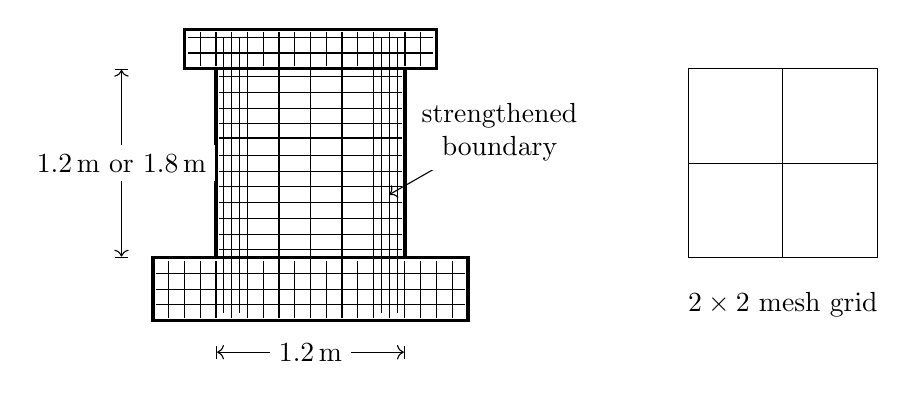
\begin{tikzpicture}[scale=2]
\draw[very thick](0,0)rectangle(1.2,1.2);
\draw[very thick](-.4,0)rectangle(1.6,-.4);
\draw[very thick](-.2,1.2)rectangle(1.4,1.45);
\foreach\x in {.05,.1,.15,.2,1.15,1.1,1.05,1,.4,.6,.8}\draw(\x,-.35)--(\x,1.4);
\foreach\x in {.05,.15,.25,.35,.45,.55,.65,.76,.85,.95,1.05,1.15}\draw(.02,\x)--(1.18,\x);
\foreach\x in {-.3,-.2,-.1,...,1.5}\draw(\x,-.38)--(\x,-.02);
\foreach\x in {-.1,0,.1,...,1.35}\draw(\x,1.22)--(\x,1.43);
\foreach\x in {-.3,-.2,-.1}\draw(-.38,\x)--(1.58,\x);
\foreach\x in {1.3,1.4}\draw(-.18,\x)--(1.38,\x);
\draw[|<->|](0,-.6)--++(1.2,0)node[midway,fill=white]{\SI{1.2}{\meter}};
\draw[|<->|](-.6,0)--++(0,1.2)node[midway,fill=white]{\SI{1.2}{\meter} or \SI{1.8}{\meter}};
\draw[<-](1.1,.4)--(1.8,.8)node[fill=white,align=center]{strengthened\\boundary};
\draw(3,0)rectangle(4.2,1.2);
\draw(3.6,0)--++(0,1.2)(3,.6)--++(1.2,0);
\node at(3.6,-.3){\numproduct{2x2} mesh grid};
\end{tikzpicture}
\caption{illustration of specimens, taken from the original paper \citep{Salonikios1999}}\label{fig:salonikios_setup}
\end{figure}

A summary of main material properties used in simulations of four specimens are listed in \tabref{tab:parameter_summary}.
\begin{table}[htb]
\setlength{\tabcolsep}{5pt}
\scriptsize\centering\caption{summary of main material parameters used in LSW1, LSW2, MSW1 and MSW2}\label{tab:parameter_summary}
\begin{tabular}{cccccccccccccc}
	\toprule
	     &        $w$        &        $h$        &        $t$        &       $f_c$       &       $f_t$       &    $\rho$     & concrete &             $g_t$             &             $g_c$             &   $a_t$   &   $a_c$   & $\bar{D}_t$ & $\bar{D}_c$ \\
	     & \si{\milli\metre} & \si{\milli\metre} & \si{\milli\metre} & \si{\mega\pascal} & \si{\mega\pascal} & \si{\percent} &          & \si{\kilo\newton\per\metre^2} & \si{\mega\newton\per\metre^2} &           &           &             &             \\ \midrule
	LSW1 &       1200        &       1200        &        100        &       23.0        &        1.7        &      1.7      &   CDP    &           \num{2.0}           &          \num{0.35}           & \num{0.5} & \num{4.0} & \num{0.50}  & \num{0.45}  \\
	LSW2 &       1200        &       1200        &        100        &       21.0        &        1.5        &      1.3      &   CDP    &           \num{1.0}           &          \num{0.20}           & \num{0.5} & \num{4.0} & \num{0.55}  & \num{0.60}  \\
	MSW1 &       1200        &       1800        &        100        &       23.0        &        1.1        &      1.2      &   CDP    &           \num{2.0}           &          \num{0.35}           & \num{0.5} & \num{4.0} & \num{0.50}  & \num{0.55}  \\
	MSW2 &       1200        &       1800        &        100        &       23.0        &        1.1        &      1.1      &   CDP    &           \num{1.3}           &          \num{0.35}           & \num{0.5} & \num{4.0} & \num{0.50}  & \num{0.55}  \\ \bottomrule
\end{tabular}
\end{table}
The following properties are not changed for all four specimens: elastic modulus $E=\SI{30}{\giga\pascal}$, Poisson's ratio $\nu=\num{0.2}$, dilatation parameter $\alpha_p=\num{0.2}$, ratio between biaxial and uniaxial compressive strengths $f_{bc}/f_c=\num{1.16}$, reinforcement yield strength $f_y=\SI{500}{\mega\pascal}$ and the corresponding hardening ratio $b=\SI{1}{\percent}$. The reinforcement ratios range from \SI{1.1}{\percent} to \SI{1.7}{\percent}. Strength degradation mainly depends on concrete response, which is controlled by material model parameters: normalised energy terms $g_t$ and $g_c$. Due to the lack of those properties, assumed values are used. They are larger than realistic values in order to stabilize the softening response, as well as to model the effect of confinement. Similar practice can be seen in the original literature \citep{Lee1996}.

As shown in \figref{fig:salonikios_wall}, loading envelops are well captured by GCMQ-L with CDP model using a \numproduct{2x2} mesh grid. The initial stiffness, as well as the descending branch, can be well captured by numerical models.
\begin{figure}[htb]
\scriptsize\centering
\begin{subfigure}[b]{.48\textwidth}
\begin{tikzpicture}[gnuplot]
%% generated with GNUPLOT 5.2p6 (Lua 5.3; terminal rev. Nov 2018, script rev. 107)
%% 03/27/2019 19:36:20
\path (0.000,0.000) rectangle (6.500,4.000);
\gpcolor{color=gp lt color border}
\gpsetlinetype{gp lt border}
\gpsetdashtype{gp dt solid}
\gpsetlinewidth{1.00}
\draw[gp path] (0.000,0.000)--(0.180,0.000);
\node[gp node right] at (-0.184,0.000) {$0$};
\draw[gp path] (0.000,0.689)--(0.090,0.689);
\draw[gp path] (0.000,1.379)--(0.180,1.379);
\node[gp node right] at (-0.184,1.379) {$1$};
\draw[gp path] (0.000,2.068)--(0.090,2.068);
\draw[gp path] (0.000,2.758)--(0.180,2.758);
\node[gp node right] at (-0.184,2.758) {$2$};
\draw[gp path] (0.000,3.447)--(0.090,3.447);
\draw[gp path] (0.000,0.000)--(0.000,0.180);
\node[gp node center] at (0.000,-0.308) {$0$};
\draw[gp path] (1.300,0.000)--(1.300,0.180);
\node[gp node center] at (1.300,-0.308) {$3$};
\draw[gp path] (2.600,0.000)--(2.600,0.180);
\node[gp node center] at (2.600,-0.308) {$6$};
\draw[gp path] (3.899,0.000)--(3.899,0.180);
\node[gp node center] at (3.899,-0.308) {$9$};
\draw[gp path] (5.199,0.000)--(5.199,0.180);
\node[gp node center] at (5.199,-0.308) {$12$};
\draw[gp path] (0.000,3.999)--(0.000,3.819);
\node[gp node center] at (0.000,4.307) {$0$};
\draw[gp path] (1.300,3.999)--(1.300,3.819);
\node[gp node center] at (1.300,4.307) {$0.25$};
\draw[gp path] (2.600,3.999)--(2.600,3.819);
\node[gp node center] at (2.600,4.307) {$0.5$};
\draw[gp path] (3.899,3.999)--(3.899,3.819);
\node[gp node center] at (3.899,4.307) {$0.75$};
\draw[gp path] (5.199,3.999)--(5.199,3.819);
\node[gp node center] at (5.199,4.307) {$1$};
\draw[gp path] (0.000,3.999)--(0.000,0.000)--(6.499,0.000)--(6.499,3.999)--cycle;
\node[gp node center,rotate=-270] at (-0.676,1.999) {base resistance (\SI{E2}{\kilo\newton})};
\node[gp node center] at (3.249,-0.769) {top displacement (\si{\milli\metre})};
\node[gp node center] at (3.249,4.769) {drift ratio (\si{\percent})};
\node[gp node right] at (5.605,3.445) {LSW1};
\gpcolor{rgb color={0.600,0.600,0.600}}
\gpsetlinewidth{2.00}
\draw[gp path] (5.789,3.445)--(6.153,3.445);
\draw[gp path] (0.000,0.480)--(0.043,0.674)--(0.082,1.055)--(0.165,1.387)--(0.182,1.578)%
  --(0.199,1.705)--(0.221,1.291)--(0.121,0.911)--(0.039,0.515)--(0.000,0.284);
\draw[gp path] (0.000,0.270)--(0.039,0.515)--(0.091,0.832)--(0.143,1.133)--(0.117,1.309)%
  --(0.165,1.499)--(0.212,1.688)--(0.225,1.370)--(0.056,0.706)--(0.004,0.000);
\draw[gp path] (0.000,0.808)--(0.030,0.881)--(0.087,1.294)--(0.152,1.594)--(0.251,1.958)%
  --(0.299,2.259)--(0.381,2.432)--(0.520,2.557)--(0.702,2.600)--(0.650,2.299)--(0.628,1.982)%
  --(0.581,1.697)--(0.420,1.287)--(0.381,0.890)--(0.238,0.670)--(0.208,0.480)--(0.204,0.258)%
  --(0.115,0.000);
\draw[gp path] (0.000,0.774)--(0.030,0.834)--(0.221,1.195)--(0.351,1.654)--(0.386,1.844)%
  --(0.464,2.081)--(0.529,2.270)--(0.594,2.444)--(0.659,2.554)--(0.784,2.869)--(0.910,3.073)%
  --(1.066,3.197)--(1.144,3.291)--(1.122,3.053)--(1.040,2.720)--(0.988,2.372)--(0.129,0.000);
\draw[gp path] (0.148,0.000)--(0.836,1.739)--(0.711,1.440)--(0.615,1.155)--(0.581,0.886)%
  --(0.420,0.587)--(0.325,0.366)--(0.260,0.224)--(0.117,0.000);
\draw[gp path] (0.041,0.000)--(0.186,0.306)--(0.334,0.780)--(0.494,1.221)--(0.594,1.696)%
  --(0.693,2.139)--(0.836,2.359)--(0.884,2.581)--(0.979,2.817)--(1.092,2.974)--(1.278,3.288)%
  --(1.434,3.460)--(1.573,3.488)--(1.646,3.344)--(1.577,2.932)--(1.508,2.567)--(1.382,2.236)%
  --(1.282,1.857)--(1.122,1.479)--(1.010,1.131)--(0.819,0.769)--(0.646,0.455)--(0.412,0.174)%
  --(0.303,0.049)--(0.216,0.000);
\draw[gp path] (0.000,0.000)--(0.095,0.180)--(0.507,1.094)--(0.728,1.582)--(0.936,1.991)%
  --(1.170,2.352)--(1.265,2.668)--(1.395,2.967)--(1.564,3.202)--(1.629,3.265)--(1.607,2.883)%
  --(1.538,2.487)--(1.486,2.298)--(1.330,1.983)--(1.230,1.683)--(1.105,1.272)--(0.932,0.974)%
  --(0.802,0.706)--(0.628,0.376)--(0.442,0.125)--(0.374,0.000);
\draw[gp path] (0.077,0.000)--(0.217,0.321)--(0.364,0.763)--(0.711,1.360)--(0.884,1.817)%
  --(1.001,2.181)--(1.278,2.540)--(1.343,2.778)--(1.469,2.998)--(1.581,3.138)--(1.603,2.804)%
  --(1.490,2.377)--(1.295,1.872)--(0.979,1.084)--(0.849,0.832)--(0.706,0.470)--(0.472,0.172)%
  --(0.334,0.000);
\draw[gp path] (0.090,0.000)--(0.277,0.320)--(0.407,0.730)--(0.615,1.139)--(0.945,1.768)%
  --(0.979,1.911)--(1.044,2.068)--(1.092,2.290)--(1.313,2.619)--(1.499,2.886)--(1.638,3.042)%
  --(1.763,3.182)--(2.010,3.352)--(2.149,3.476)--(2.366,3.583)--(2.517,3.643)--(2.574,3.451)%
  --(2.509,3.230)--(2.413,3.041)--(2.348,2.804)--(2.314,2.535)--(2.158,2.331)--(2.075,2.126)%
  --(1.997,1.937)--(1.980,1.778)--(1.824,1.511)--(1.755,1.274)--(1.664,1.229)--(1.525,1.136)%
  --(1.490,0.946)--(1.352,0.758)--(1.148,0.460)--(1.023,0.272)--(0.819,0.038)--(0.765,0.000);
\draw[gp path] (0.000,0.625)--(0.719,1.137)--(0.000,0.619);
\draw[gp path] (0.000,0.614)--(0.195,0.751)--(0.507,1.046)--(0.728,1.423)--(1.018,1.671)%
  --(1.282,1.841)--(1.438,2.171)--(1.690,2.421)--(1.906,2.718)--(2.075,2.921)--(2.266,3.140)%
  --(2.374,3.265)--(2.526,3.357)--(2.569,3.133)--(2.535,2.927)--(2.392,2.597)--(2.279,2.424)%
  --(2.136,2.061)--(2.041,1.777)--(1.898,1.589)--(3.652,2.697)--(1.664,1.101)--(1.430,0.804)%
  --(1.118,0.413)--(0.836,0.133)--(0.718,0.000);
\draw[gp path] (0.000,0.707)--(0.321,0.939)--(0.706,1.281)--(1.049,1.687)--(1.222,1.906)%
  --(1.486,2.139)--(1.638,2.294)--(1.841,2.513)--(2.119,2.761)--(2.244,2.997)--(2.448,3.152)%
  --(2.647,3.338)--(2.517,2.912)--(2.405,2.564)--(2.153,2.109)--(1.945,1.588)--(1.815,1.273)%
  --(1.586,0.976)--(1.334,0.679)--(1.100,0.350)--(0.884,0.180)--(0.693,0.000);
\draw[gp path] (0.000,0.709)--(0.043,0.754)--(0.550,1.029)--(0.815,1.294)--(0.953,1.450)%
  --(1.122,1.558)--(1.252,1.810)--(1.668,2.294)--(1.919,2.511)--(2.383,3.010)--(2.678,3.385)%
  --(2.864,3.461)--(3.076,3.473)--(3.102,3.218)--(2.912,2.904)--(2.799,2.492)--(2.699,2.161)%
  --(2.608,2.035)--(2.604,1.892)--(2.509,1.704)--(2.387,1.611)--(2.292,1.390)--(2.184,1.233)%
  --(2.028,1.062)--(1.932,0.857)--(1.807,0.653)--(1.668,0.513)--(1.542,0.404)--(1.373,0.217)%
  --(1.187,0.030)--(1.133,0.000);
\draw[gp path] (0.000,0.544)--(0.039,0.563)--(0.381,0.826)--(0.984,1.386)--(1.200,1.588)%
  --(1.369,1.696)--(2.201,2.171)--(1.646,1.913)--(1.785,2.037)--(1.989,2.223)--(2.188,2.426)%
  --(2.409,2.692)--(2.595,2.878)--(2.764,3.034)--(2.964,3.189)--(3.133,3.281)--(3.146,3.153)%
  --(3.063,2.821)--(3.029,2.647)--(2.920,2.426)--(2.825,2.174)--(2.743,1.905)--(2.539,1.592)%
  --(2.413,1.340)--(2.318,1.119)--(2.036,0.728)--(1.785,0.479)--(1.603,0.308)--(1.321,0.091)%
  --(1.160,0.000);
\draw[gp path] (0.000,0.708)--(2.240,1.916)--(0.134,0.784)--(0.533,0.982)--(0.841,1.119)%
  --(0.997,1.338)--(1.369,1.569)--(1.616,1.834)--(1.997,2.032)--(2.448,2.436)--(2.617,2.576)%
  --(2.743,2.716)--(2.899,2.904)--(3.085,3.059)--(3.280,3.055)--(3.202,2.866)--(3.185,2.707)%
  --(3.120,2.549)--(2.981,2.377)--(2.899,2.188)--(2.821,1.952)--(2.600,1.686)--(2.535,1.417)%
  --(2.379,1.134)--(2.192,0.947)--(1.989,0.681)--(1.399,0.153)--(1.200,0.000);
\draw[gp path] (0.000,0.679)--(0.165,0.751)--(0.550,0.950)--(0.871,1.150)--(1.274,1.459)%
  --(1.495,1.789)--(1.815,1.925)--(2.509,2.530)--(2.816,2.715)--(3.094,2.884)--(3.297,3.007)%
  --(3.522,3.066)--(3.661,3.126)--(3.782,3.092)--(3.687,2.887)--(3.609,2.635)--(3.509,2.366)%
  --(3.431,2.193)--(3.349,1.956)--(3.163,1.769)--(3.072,1.580)--(2.942,1.345)--(2.743,1.126)%
  --(2.691,0.905)--(2.539,0.765)--(2.353,0.578)--(2.214,0.438)--(1.980,0.268)--(1.781,0.097)%
  --(1.652,0.000);
\draw[gp path] (0.000,0.573)--(0.472,0.793)--(0.871,0.991)--(1.287,1.268)--(1.564,1.469)%
  --(1.807,1.607)--(1.993,1.794)--(2.366,2.056)--(2.578,2.179)--(2.764,2.302)--(3.042,2.503)%
  --(3.198,2.659)--(3.336,2.752)--(3.492,2.875)--(3.722,2.950)--(3.808,2.837)--(3.696,2.601)%
  --(3.587,2.412)--(3.522,2.191)--(3.379,1.956)--(3.271,1.688)--(3.189,1.435)--(3.050,1.279)%
  --(2.907,1.011)--(2.691,0.857)--(2.522,0.654)--(2.275,0.437)--(2.010,0.124)--(1.782,0.000);
\draw[gp path] (0.000,0.568)--(1.036,0.876)--(1.447,1.074)--(1.772,1.322)--(2.036,1.491)%
  --(2.283,1.677)--(2.591,1.877)--(2.808,2.047)--(3.007,2.250)--(3.176,2.437)--(3.332,2.561)%
  --(3.488,2.701)--(3.700,2.792)--(3.821,2.741)--(3.774,2.536)--(3.661,2.236)--(3.566,2.079)%
  --(3.392,1.828)--(3.237,1.529)--(3.029,1.104)--(2.799,0.823)--(2.582,0.621)--(2.288,0.341)%
  --(2.010,0.188)--(1.758,0.000);
\draw[gp path] (0.000,0.420)--(0.576,0.727)--(1.308,0.997)--(1.850,1.368)--(2.465,1.752)%
  --(2.959,2.139)--(3.301,2.514)--(4.099,2.879)--(4.311,2.938)--(4.402,2.872)--(4.354,2.635)%
  --(4.259,2.430)--(4.116,2.163)--(4.003,1.815)--(3.817,1.597)--(3.674,1.409)--(3.596,1.188)%
  --(3.423,1.032)--(3.327,0.748)--(3.154,0.450)--(2.890,0.201)--(2.418,0.020)--(2.360,0.000);
\draw[gp path] (0.000,0.428)--(0.602,0.535)--(0.940,0.687)--(1.079,0.764)--(1.248,0.840)%
  --(1.581,0.912)--(1.785,1.067)--(2.058,1.109)--(2.383,1.388)--(2.643,1.494)--(2.903,1.648)%
  --(3.059,1.787)--(3.631,2.189)--(3.817,2.408)--(4.016,2.530)--(4.172,2.670)--(4.367,2.730)%
  --(0.000,0.208);
\draw[gp path] (0.000,0.098)--(4.346,2.380)--(4.237,2.128)--(4.107,1.845)--(3.969,1.657)%
  --(3.951,1.546)--(3.886,1.309)--(3.730,1.137)--(3.574,0.997)--(3.345,0.780)--(3.176,0.656)%
  --(3.050,0.563)--(2.912,0.375)--(2.725,0.252)--(2.387,0.084)--(2.237,0.000);
\draw[gp path] (0.000,0.460)--(0.160,0.497)--(0.849,0.641)--(1.382,0.789)--(1.794,0.860)%
  --(2.179,1.059)--(2.591,1.273)--(2.933,1.552)--(3.457,1.874)--(3.735,2.123)--(3.995,2.308)%
  --(4.229,2.510)--(4.411,2.618)--(4.502,2.552)--(4.376,2.300)--(4.263,2.048)--(4.198,1.827)%
  --(3.982,1.466)--(3.713,1.090)--(3.618,0.917)--(3.479,0.697)--(3.172,0.481)--(2.938,0.295)%
  --(2.634,0.175)--(2.359,0.000);
\gpcolor{color=gp lt color border}
\node[gp node right] at (5.605,3.137) {GCMQ-L};
\gpcolor{rgb color={1.000,0.000,0.000}}
\gpsetlinewidth{4.00}
\draw[gp path] (5.789,3.137)--(6.153,3.137);
\draw[gp path] (0.000,0.000)--(0.013,0.208)--(0.026,0.416)--(0.039,0.621)--(0.052,0.787)%
  --(0.065,0.952)--(0.078,1.069)--(0.091,1.162)--(0.104,1.246)--(0.117,1.320)--(0.130,1.379)%
  --(0.143,1.437)--(0.156,1.493)--(0.169,1.549)--(0.182,1.604)--(0.195,1.658)--(0.208,1.713)%
  --(0.221,1.765)--(0.234,1.815)--(0.247,1.863)--(0.260,1.906)--(0.273,1.948)--(0.286,1.991)%
  --(0.299,2.034)--(0.312,2.071)--(0.325,2.106)--(0.338,2.139)--(0.351,2.170)--(0.364,2.204)%
  --(0.377,2.235)--(0.390,2.268)--(0.403,2.300)--(0.416,2.332)--(0.429,2.362)--(0.442,2.393)%
  --(0.455,2.421)--(0.468,2.450)--(0.481,2.478)--(0.494,2.507)--(0.507,2.535)--(0.520,2.561)%
  --(0.533,2.588)--(0.546,2.613)--(0.559,2.637)--(0.572,2.659)--(0.585,2.678)--(0.598,2.697)%
  --(0.611,2.717)--(0.624,2.736)--(0.637,2.754)--(0.650,2.772)--(0.663,2.788)--(0.676,2.806)%
  --(0.689,2.823)--(0.702,2.839)--(0.715,2.857)--(0.728,2.874)--(0.741,2.890)--(0.754,2.905)%
  --(0.767,2.919)--(0.780,2.934)--(0.793,2.948)--(0.806,2.962)--(0.819,2.976)--(0.832,2.988)%
  --(0.845,3.002)--(0.858,3.016)--(0.871,3.028)--(0.884,3.041)--(0.897,3.053)--(0.910,3.065)%
  --(0.923,3.078)--(0.936,3.090)--(0.949,3.101)--(0.962,3.114)--(0.975,3.125)--(0.988,3.136)%
  --(1.001,3.148)--(1.014,3.159)--(1.027,3.170)--(1.040,3.180)--(1.053,3.191)--(1.066,3.202)%
  --(1.079,3.212)--(1.092,3.223)--(1.105,3.232)--(1.118,3.242)--(1.131,3.252)--(1.144,3.261)%
  --(1.157,3.271)--(1.170,3.281)--(1.183,3.290)--(1.196,3.298)--(1.209,3.308)--(1.222,3.316)%
  --(1.235,3.326)--(1.248,3.334)--(1.261,3.343)--(1.274,3.351)--(1.287,3.359)--(1.300,3.367)%
  --(1.313,3.376)--(1.326,3.383)--(1.339,3.391)--(1.352,3.398)--(1.365,3.406)--(1.378,3.413)%
  --(1.391,3.420)--(1.404,3.428)--(1.417,3.435)--(1.430,3.442)--(1.443,3.447)--(1.456,3.454)%
  --(1.469,3.461)--(1.482,3.468)--(1.495,3.474)--(1.508,3.481)--(1.521,3.486)--(1.534,3.492)%
  --(1.547,3.497)--(1.560,3.503)--(1.573,3.509)--(1.586,3.514)--(1.599,3.519)--(1.612,3.525)%
  --(1.625,3.530)--(1.638,3.536)--(1.651,3.540)--(1.664,3.545)--(1.677,3.549)--(1.690,3.554)%
  --(1.703,3.558)--(1.716,3.563)--(1.729,3.567)--(1.742,3.572)--(1.755,3.576)--(1.768,3.580)%
  --(1.781,3.583)--(1.794,3.587)--(1.807,3.591)--(1.820,3.594)--(1.833,3.598)--(1.846,3.600)%
  --(1.859,3.603)--(1.872,3.607)--(1.885,3.610)--(1.898,3.613)--(1.911,3.616)--(1.924,3.618)%
  --(1.937,3.621)--(1.950,3.624)--(1.963,3.627)--(1.976,3.628)--(1.989,3.631)--(2.002,3.632)%
  --(2.015,3.635)--(2.028,3.636)--(2.041,3.639)--(2.054,3.640)--(2.067,3.642)--(2.080,3.643)%
  --(2.093,3.646)--(2.106,3.647)--(2.119,3.649)--(2.132,3.649)--(2.145,3.650)--(2.158,3.652)%
  --(2.171,3.653)--(2.184,3.653)--(2.197,3.654)--(2.210,3.654)--(2.223,3.656)--(2.236,3.656)%
  --(2.249,3.657)--(2.262,3.657)--(2.275,3.657)--(2.288,3.657)--(2.301,3.657)--(2.314,3.657)%
  --(2.327,3.657)--(2.340,3.657)--(2.353,3.657)--(2.366,3.657)--(2.379,3.657)--(2.392,3.656)%
  --(2.405,3.656)--(2.418,3.654)--(2.431,3.654)--(2.444,3.653)--(2.457,3.653)--(2.470,3.652)%
  --(2.483,3.650)--(2.496,3.650)--(2.509,3.649)--(2.522,3.647)--(2.535,3.646)--(2.548,3.645)%
  --(2.561,3.643)--(2.574,3.642)--(2.587,3.639)--(2.600,3.638)--(2.613,3.636)--(2.626,3.635)%
  --(2.639,3.632)--(2.652,3.631)--(2.665,3.628)--(2.678,3.627)--(2.691,3.624)--(2.704,3.621)%
  --(2.717,3.620)--(2.730,3.617)--(2.743,3.614)--(2.756,3.612)--(2.769,3.609)--(2.782,3.606)%
  --(2.795,3.603)--(2.808,3.600)--(2.821,3.598)--(2.834,3.595)--(2.847,3.592)--(2.860,3.589)%
  --(2.873,3.585)--(2.886,3.583)--(2.899,3.578)--(2.912,3.576)--(2.925,3.573)--(2.938,3.569)%
  --(2.951,3.565)--(2.964,3.562)--(2.977,3.558)--(2.990,3.554)--(3.003,3.551)--(3.016,3.547)%
  --(3.029,3.543)--(3.042,3.538)--(3.055,3.534)--(3.068,3.530)--(3.081,3.526)--(3.094,3.522)%
  --(3.107,3.516)--(3.120,3.512)--(3.133,3.508)--(3.146,3.503)--(3.159,3.498)--(3.172,3.493)%
  --(3.185,3.489)--(3.198,3.483)--(3.211,3.478)--(3.224,3.474)--(3.237,3.468)--(3.250,3.463)%
  --(3.262,3.457)--(3.275,3.452)--(3.288,3.446)--(3.301,3.441)--(3.314,3.435)--(3.327,3.429)%
  --(3.340,3.423)--(3.353,3.417)--(3.366,3.412)--(3.379,3.405)--(3.392,3.399)--(3.405,3.392)%
  --(3.418,3.385)--(3.431,3.380)--(3.444,3.373)--(3.457,3.366)--(3.470,3.361)--(3.483,3.354)%
  --(3.496,3.347)--(3.509,3.340)--(3.522,3.333)--(3.535,3.326)--(3.548,3.318)--(3.561,3.311)%
  --(3.574,3.304)--(3.587,3.296)--(3.600,3.289)--(3.613,3.281)--(3.626,3.274)--(3.639,3.265)%
  --(3.652,3.258)--(3.665,3.250)--(3.678,3.242)--(3.691,3.234)--(3.704,3.225)--(3.717,3.217)%
  --(3.730,3.209)--(3.743,3.201)--(3.756,3.192)--(3.769,3.184)--(3.782,3.176)--(3.795,3.166)%
  --(3.808,3.158)--(3.821,3.150)--(3.834,3.140)--(3.847,3.132)--(3.860,3.122)--(3.873,3.112)%
  --(3.886,3.104)--(3.899,3.094)--(3.912,3.085)--(3.925,3.075)--(3.938,3.065)--(3.951,3.057)%
  --(3.964,3.048)--(3.977,3.038)--(3.990,3.028)--(4.003,3.019)--(4.016,3.009)--(4.029,2.998)%
  --(4.042,2.988)--(4.055,2.979)--(4.068,2.969)--(4.081,2.958)--(4.094,2.948)--(4.107,2.939)%
  --(4.120,2.928)--(4.133,2.918)--(4.146,2.908)--(4.159,2.897)--(4.172,2.888)--(4.185,2.877)%
  --(4.198,2.867)--(4.211,2.856)--(4.224,2.845)--(4.237,2.835)--(4.250,2.824)--(4.263,2.813)%
  --(4.276,2.803)--(4.289,2.792)--(4.302,2.781)--(4.315,2.770)--(4.328,2.759)--(4.341,2.748)%
  --(4.354,2.737)--(4.367,2.728)--(4.380,2.717)--(4.393,2.706)--(4.406,2.694)--(4.419,2.683)%
  --(4.432,2.671)--(4.445,2.660)--(4.458,2.649)--(4.471,2.638)--(4.484,2.627)--(4.497,2.616)%
  --(4.510,2.605)--(4.523,2.594)--(4.536,2.581)--(4.549,2.570)--(4.562,2.559)--(4.575,2.548)%
  --(4.588,2.536)--(4.601,2.525)--(4.614,2.514)--(4.627,2.503)--(4.640,2.490)--(4.653,2.479)%
  --(4.666,2.468)--(4.679,2.456)--(4.692,2.445)--(4.705,2.434)--(4.718,2.421)--(4.731,2.410)%
  --(4.744,2.399)--(4.757,2.387)--(4.770,2.376)--(4.783,2.365)--(4.796,2.353)--(4.809,2.341)%
  --(4.822,2.329)--(4.835,2.318)--(4.848,2.307)--(4.861,2.295)--(4.874,2.284)--(4.887,2.273)%
  --(4.900,2.260)--(4.913,2.249)--(4.926,2.237)--(4.939,2.226)--(4.952,2.215)--(4.965,2.202)%
  --(4.978,2.191)--(4.991,2.180)--(5.004,2.168)--(5.017,2.157)--(5.030,2.146)--(5.043,2.133)%
  --(5.056,2.122)--(5.069,2.111)--(5.082,2.099)--(5.095,2.088)--(5.108,2.077)--(5.121,2.064)%
  --(5.134,2.053)--(5.147,2.042)--(5.160,2.031)--(5.173,2.019)--(5.186,2.008)--(5.199,1.997);
\gpcolor{color=gp lt color border}
\gpsetlinewidth{1.00}
\draw[gp path] (0.000,3.999)--(0.000,0.000)--(6.499,0.000)--(6.499,3.999)--cycle;
\node at(5.5,1.2){
\begin{tikzpicture}
\coordinate(N1)at(0,0);
\coordinate(N2)at(.5,0);
\coordinate(N3)at(1,0);
\coordinate(N4)at(0,.5);
\coordinate(N5)at(.5,.5);
\coordinate(N6)at(1,.5);
\coordinate(N7)at(0,1);
\coordinate(N8)at(.5,1);
\coordinate(N9)at(1,1);
\draw[line width=.2mm](N1)--(N2)--(N3)--(N6)--(N9)--(N8)--(N7)--(N4)--cycle;
\draw[line width=.2mm](N2)--(N5)--(N8)(N4)--(N5)--(N6);
\FixedSupport{.5,0}{1.8}
\draw[->](.1,1.2)--++(.8,0)node[midway,anchor=south]{$u$};
\end{tikzpicture}
};
%% coordinates of the plot area
\gpdefrectangularnode{gp plot 1}{\pgfpoint{0.000cm}{0.000cm}}{\pgfpoint{6.499cm}{3.999cm}}
\end{tikzpicture}
%% gnuplot variables

\caption{LSW1 specimen}\label{fig:lsw1_pushover}
\end{subfigure}\quad
\begin{subfigure}[b]{.48\textwidth}
\begin{tikzpicture}[gnuplot]
%% generated with GNUPLOT 5.2p6 (Lua 5.3; terminal rev. Nov 2018, script rev. 107)
%% 03/27/2019 19:39:07
\path (0.000,0.000) rectangle (6.500,4.000);
\gpcolor{color=gp lt color border}
\gpsetlinetype{gp lt border}
\gpsetdashtype{gp dt solid}
\gpsetlinewidth{1.00}
\draw[gp path] (0.000,0.000)--(0.180,0.000);
\node[gp node right] at (-0.184,0.000) {$0$};
\draw[gp path] (0.000,0.909)--(0.090,0.909);
\draw[gp path] (0.000,1.818)--(0.180,1.818);
\node[gp node right] at (-0.184,1.818) {$1$};
\draw[gp path] (0.000,2.727)--(0.090,2.727);
\draw[gp path] (0.000,3.635)--(0.180,3.635);
\node[gp node right] at (-0.184,3.635) {$2$};
\draw[gp path] (0.000,0.000)--(0.000,0.180);
\node[gp node center] at (0.000,-0.308) {$0$};
\draw[gp path] (1.300,0.000)--(1.300,0.180);
\node[gp node center] at (1.300,-0.308) {$3$};
\draw[gp path] (2.600,0.000)--(2.600,0.180);
\node[gp node center] at (2.600,-0.308) {$6$};
\draw[gp path] (3.899,0.000)--(3.899,0.180);
\node[gp node center] at (3.899,-0.308) {$9$};
\draw[gp path] (5.199,0.000)--(5.199,0.180);
\node[gp node center] at (5.199,-0.308) {$12$};
\draw[gp path] (0.000,3.999)--(0.000,3.819);
\node[gp node center] at (0.000,4.307) {$0$};
\draw[gp path] (1.300,3.999)--(1.300,3.819);
\node[gp node center] at (1.300,4.307) {$0.25$};
\draw[gp path] (2.600,3.999)--(2.600,3.819);
\node[gp node center] at (2.600,4.307) {$0.5$};
\draw[gp path] (3.899,3.999)--(3.899,3.819);
\node[gp node center] at (3.899,4.307) {$0.75$};
\draw[gp path] (5.199,3.999)--(5.199,3.819);
\node[gp node center] at (5.199,4.307) {$1$};
\draw[gp path] (0.000,3.999)--(0.000,0.000)--(6.499,0.000)--(6.499,3.999)--cycle;
\node[gp node center,rotate=-270] at (-0.676,1.999) {base resistance (\SI{E2}{\kilo\newton})};
\node[gp node center] at (3.249,-0.769) {top displacement (\si{\milli\metre})};
\node[gp node center] at (3.249,4.769) {drift ratio (\si{\percent})};
\node[gp node right] at (5.605,3.445) {LSW2};
\gpcolor{rgb color={0.600,0.600,0.600}}
\gpsetlinewidth{2.00}
\draw[gp path] (5.789,3.445)--(6.153,3.445);
\draw[gp path] (0.000,0.571)--(0.002,0.602)--(0.039,0.845)--(0.092,1.088)--(0.177,1.279)%
  --(0.197,1.453)--(0.217,1.697)--(0.263,1.469)--(0.258,1.207)--(0.204,0.912)--(0.084,0.617)%
  --(0.045,0.269)--(0.042,0.095)--(0.021,0.000);
\draw[gp path] (0.000,0.491)--(0.017,0.514)--(0.320,0.089)--(0.159,1.174)--(0.216,1.592)%
  --(0.254,1.905)--(0.322,2.078)--(0.391,2.269)--(0.460,2.441)--(0.510,2.494)--(0.757,2.576)%
  --(0.719,2.298)--(0.680,1.949)--(0.610,1.671)--(0.524,1.446)--(0.388,1.152)--(0.286,0.945)%
  --(0.266,0.736)--(0.263,0.544)--(0.192,0.284)--(0.073,0.024)--(0.068,0.000);
\draw[gp path] (0.000,0.625)--(0.088,0.827)--(0.245,1.382)--(0.365,1.711)--(0.485,2.005)%
  --(0.623,2.439)--(0.641,2.508)--(0.669,2.229)--(0.597,1.847)--(0.477,1.534)--(0.355,1.136)%
  --(0.201,0.790)--(0.167,0.668)--(0.048,0.426)--(0.000,0.291);
\draw[gp path] (0.000,0.703)--(0.186,0.860)--(0.423,1.274)--(0.476,1.499)--(0.597,1.863)%
  --(0.701,2.229)--(0.739,2.488)--(0.759,2.716)--(0.928,3.008)--(1.045,3.146)--(1.194,3.212)%
  --(1.107,2.936)--(1.068,2.605)--(1.032,2.414)--(0.876,1.927)--(0.787,1.511)--(0.683,1.199)%
  --(0.647,0.990)--(0.544,0.713)--(0.474,0.505)--(0.374,0.385)--(0.240,0.195)--(0.128,0.000);
\draw[gp path] (0.000,0.449)--(1.983,2.534)--(0.443,1.483)--(0.597,1.847)--(0.700,2.158)%
  --(0.802,2.365)--(0.955,2.694)--(1.108,2.987)--(1.259,3.228)--(1.409,3.348)--(1.591,3.485)%
  --(1.654,3.361)--(1.666,3.097)--(1.645,2.819)--(1.541,2.507)--(1.420,2.127)--(1.267,1.815)%
  --(1.147,1.521)--(1.028,1.244)--(0.890,0.845)--(0.689,0.588)--(0.503,0.260)--(0.171,0.005)%
  --(0.166,0.000);
\draw[gp path] (0.000,0.729)--(0.303,0.997)--(0.487,1.220)--(0.740,1.599)--(0.925,1.892)%
  --(1.027,2.134)--(1.247,2.530)--(1.432,2.823)--(1.534,3.014)--(1.668,3.221)--(1.628,2.819)%
  --(1.506,2.403)--(1.370,2.058)--(1.233,1.728)--(1.130,1.469)--(1.043,1.209)--(0.956,0.897)%
  --(0.922,0.827)--(0.721,0.535)--(0.536,0.294)--(0.377,0.000);
\draw[gp path] (0.000,0.531)--(0.150,0.686)--(0.352,0.961)--(0.652,1.321)--(0.890,1.805)%
  --(1.211,2.358)--(1.331,2.652)--(1.498,2.857)--(1.584,3.099)--(1.702,3.290)--(1.630,2.907)%
  --(0.089,0.000);
\draw[gp path] (0.139,0.000)--(1.369,2.039)--(1.232,1.711)--(1.128,1.364)--(0.958,1.036)%
  --(0.872,0.759)--(0.620,0.397)--(0.452,0.139)--(0.386,0.000);
\draw[gp path] (0.000,0.549)--(0.085,0.670)--(0.570,1.271)--(1.006,1.856)--(1.126,2.201)%
  --(1.279,2.496)--(1.498,2.839)--(1.650,3.134)--(1.752,3.323)--(1.868,3.390)--(1.967,3.475)%
  --(2.147,3.437)--(2.110,3.212)--(2.057,2.987)--(1.955,2.777)--(1.919,2.605)--(1.900,2.430)%
  --(1.832,2.292)--(1.795,2.067)--(1.662,1.929)--(1.558,1.600)--(1.487,1.305)--(1.367,0.993)%
  --(1.133,0.718)--(0.998,0.477)--(0.815,0.289)--(0.597,0.049)--(0.540,0.000);
\draw[gp path] (0.000,0.707)--(0.020,0.723)--(0.254,0.998)--(0.438,1.186)--(0.923,1.804)%
  --(1.123,2.027)--(1.225,2.218)--(1.440,2.352)--(1.591,2.576)--(1.726,2.801)--(1.794,2.921)%
  --(1.944,3.057)--(2.027,3.161)--(2.109,3.141)--(2.139,3.001)--(2.036,2.759)--(1.961,2.219)%
  --(1.876,1.994)--(1.740,1.753)--(1.704,1.562)--(1.569,1.338)--(1.450,1.078)--(1.299,0.855)%
  --(1.131,0.596)--(0.963,0.338)--(0.779,0.132)--(0.631,0.000);
\draw[gp path] (0.000,0.795)--(0.155,0.948)--(0.769,1.424)--(1.037,1.767)--(1.221,1.956)%
  --(1.422,2.230)--(1.491,2.456)--(1.607,2.559)--(1.790,2.712)--(2.007,2.970)--(2.104,2.845)%
  --(2.083,2.601)--(2.014,2.410)--(1.875,1.943)--(1.754,1.613)--(1.584,1.250)--(1.415,0.957)%
  --(1.198,0.665)--(1.013,0.407)--(0.813,0.201)--(0.585,0.000);
\draw[gp path] (0.000,0.711)--(0.553,1.219)--(0.886,1.579)--(1.221,2.009)--(1.438,2.249)%
  --(1.556,2.419)--(1.706,2.556)--(2.005,2.830)--(2.189,3.036)--(2.289,3.137)--(2.470,3.221)%
  --(2.536,3.272)--(2.667,3.270)--(2.732,3.234)--(2.680,3.061)--(2.578,2.817)--(2.525,2.610)%
  --(2.403,2.229)--(2.249,1.830)--(0.351,0.000);
\draw[gp path] (0.586,0.000)--(1.925,1.104)--(1.741,0.846)--(1.623,0.674)--(1.439,0.451)%
  --(1.173,0.229)--(0.886,0.000);
\draw[gp path] (0.000,0.847)--(0.255,1.068)--(0.802,1.423)--(1.086,1.766)--(1.418,2.003)%
  --(1.668,2.278)--(2.233,2.756)--(2.432,2.943)--(2.631,3.045)--(2.711,2.972)--(2.707,2.747)%
  --(2.621,2.503)--(2.435,2.158)--(2.264,1.725)--(2.110,1.362)--(1.940,0.981)--(1.623,0.656)%
  --(1.389,0.399)--(1.140,0.195)--(0.875,0.000);
\draw[gp path] (0.000,0.728)--(0.549,0.992)--(0.882,1.317)--(1.264,1.658)--(1.597,1.983)%
  --(1.830,2.205)--(2.129,2.443)--(2.312,2.598)--(2.510,2.716)--(2.709,2.834)--(2.569,2.330)%
  --(2.415,1.949)--(2.262,1.621)--(2.126,1.361)--(1.925,1.086)--(1.739,0.741)--(1.471,0.432)%
  --(1.139,0.160)--(0.916,0.000);
\draw[gp path] (0.000,0.822)--(0.336,1.014)--(0.734,1.268)--(1.114,1.521)--(1.381,1.778)%
  --(1.696,2.034)--(2.012,2.270)--(2.194,2.407)--(2.327,2.527)--(2.380,2.736)--(2.431,2.856)%
  --(2.612,2.887)--(2.827,3.039)--(3.073,3.070)--(3.236,3.014)--(3.215,2.788)--(3.178,2.545)%
  --(3.074,2.216)--(2.939,1.956)--(2.836,1.696)--(2.700,1.402)--(2.665,1.281)--(2.516,1.162)%
  --(2.365,0.973)--(2.346,0.834)--(2.279,0.765)--(2.114,0.664)--(1.964,0.492)--(1.796,0.286)%
  --(1.664,0.184)--(1.531,0.100)--(1.400,0.000);
\draw[gp path] (0.000,0.529)--(0.428,0.645)--(0.000,0.535);
\draw[gp path] (0.000,0.708)--(0.649,1.147)--(1.214,1.624)--(1.661,1.878)--(2.074,2.112)%
  --(2.422,2.385)--(2.720,2.570)--(3.067,2.703)--(3.297,2.787)--(3.362,2.768)--(3.342,2.559)%
  --(3.306,2.367)--(3.170,2.056)--(3.084,1.830)--(3.063,1.604)--(2.929,1.415)--(2.862,1.294)%
  --(2.679,1.141)--(2.578,0.986)--(2.527,0.882)--(2.475,0.726)--(2.342,0.607)--(2.143,0.419)%
  --(1.861,0.233)--(1.562,0.012)--(1.536,0.000);
\draw[gp path] (0.000,0.706)--(0.283,0.771)--(0.629,0.903)--(0.958,1.019)--(1.191,1.223)%
  --(1.521,1.391)--(1.804,1.665)--(2.052,1.782)--(2.283,1.916)--(2.714,2.187)--(2.896,2.341)%
  --(3.111,2.458)--(3.309,2.559)--(3.375,2.576)--(3.372,2.401)--(3.301,2.089)--(3.215,1.829)%
  --(3.128,1.568)--(2.894,1.259)--(2.758,0.982)--(2.541,0.760)--(2.076,0.385)--(1.827,0.164)%
  --(1.489,0.000);
\draw[gp path] (0.000,0.648)--(0.529,0.783)--(1.025,1.087)--(1.120,0.928)--(1.584,1.215)%
  --(2.179,1.570)--(2.461,1.791)--(2.594,1.910)--(2.725,1.925)--(2.810,2.063)--(2.942,2.165)%
  --(3.157,2.283)--(3.422,2.434)--(3.670,2.587)--(3.850,2.618)--(3.948,2.563)--(4.042,2.370)%
  --(4.139,2.263)--(4.136,2.089)--(4.099,1.880)--(3.948,1.656)--(3.846,1.449)--(3.711,1.225)%
  --(3.577,1.036)--(3.442,0.812)--(3.275,0.623)--(2.962,0.507)--(2.762,0.267)--(2.414,0.030)%
  --(2.335,0.000);
\draw[gp path] (0.000,0.595)--(0.018,0.601)--(0.823,0.777)--(1.433,1.044)--(1.795,1.124)%
  --(2.092,1.275)--(2.440,1.512)--(2.672,1.647)--(3.051,1.849)--(3.349,2.000)--(3.614,2.221)%
  --(3.846,2.339)--(3.945,2.407)--(3.808,2.043)--(3.655,1.715)--(3.435,1.353)--(3.249,0.990)%
  --(3.014,0.646)--(2.763,0.337)--(2.349,0.083)--(2.106,0.000);
\draw[gp path] (0.000,0.492)--(0.247,0.597)--(0.937,0.722)--(1.412,0.800)--(1.808,0.984)%
  --(2.221,1.185)--(2.568,1.335)--(2.948,1.572)--(3.262,1.757)--(3.545,1.996)--(3.909,2.216)%
  --(4.090,2.299)--(3.972,2.074)--(3.969,1.900)--(3.949,1.726)--(3.800,1.625)--(3.666,1.435)%
  --(3.598,1.279)--(3.578,1.105)--(3.413,1.004)--(3.262,0.798)--(3.095,0.627)--(2.879,0.439)%
  --(2.615,0.287)--(2.192,0.000);
\draw[gp path] (0.000,0.503)--(1.396,0.818)--(2.287,1.184)--(2.766,1.453)--(3.328,1.791)%
  --(3.759,2.061)--(4.040,2.230)--(4.271,2.330)--(4.450,2.379)--(4.536,2.447)--(4.614,2.323)%
  --(4.662,2.201)--(4.510,1.925)--(4.424,1.629)--(4.337,1.474)--(4.220,1.302)--(4.102,1.130)%
  --(4.068,1.008)--(3.900,0.802)--(3.701,0.614)--(3.518,0.461)--(3.353,0.395)--(3.154,0.259)%
  --(2.955,0.106)--(2.724,0.023)--(2.634,0.000);
\gpcolor{color=gp lt color border}
\node[gp node right] at (5.605,3.137) {GCMQ-L};
\gpcolor{rgb color={1.000,0.000,0.000}}
\gpsetlinewidth{4.00}
\draw[gp path] (5.789,3.137)--(6.153,3.137);
\draw[gp path] (0.000,0.000)--(0.013,0.270)--(0.026,0.540)--(0.039,0.787)--(0.052,0.998)%
  --(0.065,1.171)--(0.078,1.285)--(0.091,1.380)--(0.104,1.457)--(0.117,1.513)--(0.130,1.565)%
  --(0.143,1.615)--(0.156,1.664)--(0.169,1.713)--(0.182,1.762)--(0.195,1.810)--(0.208,1.856)%
  --(0.221,1.903)--(0.234,1.949)--(0.247,1.996)--(0.260,2.039)--(0.273,2.078)--(0.286,2.112)%
  --(0.299,2.145)--(0.312,2.178)--(0.325,2.210)--(0.338,2.243)--(0.351,2.278)--(0.364,2.312)%
  --(0.377,2.347)--(0.390,2.381)--(0.403,2.416)--(0.416,2.450)--(0.429,2.483)--(0.442,2.516)%
  --(0.455,2.548)--(0.468,2.581)--(0.481,2.614)--(0.494,2.643)--(0.507,2.672)--(0.520,2.699)%
  --(0.533,2.725)--(0.546,2.750)--(0.559,2.774)--(0.572,2.799)--(0.585,2.821)--(0.598,2.845)%
  --(0.611,2.867)--(0.624,2.888)--(0.637,2.910)--(0.650,2.930)--(0.663,2.950)--(0.676,2.970)%
  --(0.689,2.988)--(0.702,3.007)--(0.715,3.027)--(0.728,3.043)--(0.741,3.057)--(0.754,3.072)%
  --(0.767,3.087)--(0.780,3.101)--(0.793,3.116)--(0.806,3.128)--(0.819,3.141)--(0.832,3.154)%
  --(0.845,3.166)--(0.858,3.179)--(0.871,3.192)--(0.884,3.205)--(0.897,3.217)--(0.910,3.228)%
  --(0.923,3.241)--(0.936,3.252)--(0.949,3.263)--(0.962,3.274)--(0.975,3.283)--(0.988,3.292)%
  --(1.001,3.301)--(1.014,3.310)--(1.027,3.319)--(1.040,3.328)--(1.053,3.337)--(1.066,3.345)%
  --(1.079,3.354)--(1.092,3.361)--(1.105,3.368)--(1.118,3.377)--(1.131,3.385)--(1.144,3.392)%
  --(1.157,3.399)--(1.170,3.406)--(1.183,3.412)--(1.196,3.419)--(1.209,3.425)--(1.222,3.432)%
  --(1.235,3.437)--(1.248,3.443)--(1.261,3.448)--(1.274,3.454)--(1.287,3.459)--(1.300,3.465)%
  --(1.313,3.470)--(1.326,3.475)--(1.339,3.479)--(1.352,3.485)--(1.365,3.488)--(1.378,3.492)%
  --(1.391,3.495)--(1.404,3.499)--(1.417,3.503)--(1.430,3.506)--(1.443,3.510)--(1.456,3.514)%
  --(1.469,3.515)--(1.482,3.519)--(1.495,3.521)--(1.508,3.523)--(1.521,3.526)--(1.534,3.528)%
  --(1.547,3.530)--(1.560,3.532)--(1.573,3.534)--(1.586,3.535)--(1.599,3.535)--(1.612,3.537)%
  --(1.625,3.539)--(1.638,3.539)--(1.651,3.539)--(1.664,3.541)--(1.677,3.541)--(1.690,3.541)%
  --(1.703,3.541)--(1.716,3.541)--(1.729,3.541)--(1.742,3.541)--(1.755,3.541)--(1.768,3.539)%
  --(1.781,3.539)--(1.794,3.539)--(1.807,3.537)--(1.820,3.535)--(1.833,3.535)--(1.846,3.534)%
  --(1.859,3.532)--(1.872,3.530)--(1.885,3.528)--(1.898,3.526)--(1.911,3.525)--(1.924,3.523)%
  --(1.937,3.521)--(1.950,3.519)--(1.963,3.517)--(1.976,3.514)--(1.989,3.512)--(2.002,3.508)%
  --(2.015,3.506)--(2.028,3.503)--(2.041,3.499)--(2.054,3.497)--(2.067,3.494)--(2.080,3.490)%
  --(2.093,3.486)--(2.106,3.483)--(2.119,3.479)--(2.132,3.475)--(2.145,3.472)--(2.158,3.468)%
  --(2.171,3.465)--(2.184,3.461)--(2.197,3.457)--(2.210,3.452)--(2.223,3.448)--(2.236,3.445)%
  --(2.249,3.439)--(2.262,3.436)--(2.275,3.430)--(2.288,3.426)--(2.301,3.421)--(2.314,3.417)%
  --(2.327,3.412)--(2.340,3.408)--(2.353,3.403)--(2.366,3.397)--(2.379,3.392)--(2.392,3.388)%
  --(2.405,3.383)--(2.418,3.377)--(2.431,3.372)--(2.444,3.366)--(2.457,3.363)--(2.470,3.357)%
  --(2.483,3.352)--(2.496,3.346)--(2.509,3.341)--(2.522,3.336)--(2.535,3.330)--(2.548,3.325)%
  --(2.561,3.319)--(2.574,3.314)--(2.587,3.306)--(2.600,3.301)--(2.613,3.296)--(2.626,3.290)%
  --(2.639,3.285)--(2.652,3.279)--(2.665,3.274)--(2.678,3.266)--(2.691,3.261)--(2.704,3.256)%
  --(2.717,3.250)--(2.730,3.245)--(2.743,3.237)--(2.756,3.232)--(2.769,3.226)--(2.782,3.221)%
  --(2.795,3.214)--(2.808,3.208)--(2.821,3.203)--(2.834,3.196)--(2.847,3.190)--(2.860,3.183)%
  --(2.873,3.177)--(2.886,3.172)--(2.899,3.165)--(2.912,3.159)--(2.925,3.152)--(2.938,3.146)%
  --(2.951,3.139)--(2.964,3.134)--(2.977,3.126)--(2.990,3.121)--(3.003,3.114)--(3.016,3.108)%
  --(3.029,3.101)--(3.042,3.096)--(3.055,3.088)--(3.068,3.081)--(3.081,3.076)--(3.094,3.068)%
  --(3.107,3.063)--(3.120,3.056)--(3.133,3.048)--(3.146,3.043)--(3.159,3.036)--(3.172,3.028)%
  --(3.185,3.021)--(3.198,3.016)--(3.211,3.008)--(3.224,3.001)--(3.237,2.994)--(3.250,2.988)%
  --(3.262,2.981)--(3.275,2.974)--(3.288,2.967)--(3.301,2.959)--(3.314,2.954)--(3.327,2.947)%
  --(3.340,2.939)--(3.353,2.932)--(3.366,2.925)--(3.379,2.917)--(3.392,2.910)--(3.405,2.903)%
  --(3.418,2.896)--(3.431,2.888)--(3.444,2.881)--(3.457,2.872)--(3.470,2.865)--(3.483,2.857)%
  --(3.496,2.850)--(3.509,2.843)--(3.522,2.836)--(3.535,2.827)--(3.548,2.819)--(3.561,2.812)%
  --(3.574,2.805)--(3.587,2.796)--(3.600,2.788)--(3.613,2.781)--(3.626,2.772)--(3.639,2.765)%
  --(3.652,2.756)--(3.665,2.748)--(3.678,2.739)--(3.691,2.732)--(3.704,2.723)--(3.717,2.714)%
  --(3.730,2.707)--(3.743,2.698)--(3.756,2.690)--(3.769,2.681)--(3.782,2.672)--(3.795,2.663)%
  --(3.808,2.656)--(3.821,2.647)--(3.834,2.638)--(3.847,2.628)--(3.860,2.619)--(3.873,2.612)%
  --(3.886,2.603)--(3.899,2.594)--(3.912,2.585)--(3.925,2.576)--(3.938,2.567)--(3.951,2.558)%
  --(3.964,2.548)--(3.977,2.539)--(3.990,2.530)--(4.003,2.521)--(4.016,2.510)--(4.029,2.501)%
  --(4.042,2.492)--(4.055,2.483)--(4.068,2.472)--(4.081,2.463)--(4.094,2.454)--(4.107,2.443)%
  --(4.120,2.434)--(4.133,2.425)--(4.146,2.414)--(4.159,2.405)--(4.172,2.394)--(4.185,2.385)%
  --(4.198,2.374)--(4.211,2.365)--(4.224,2.354)--(4.237,2.345)--(4.250,2.334)--(4.263,2.325)%
  --(4.276,2.314)--(4.289,2.303)--(4.302,2.294)--(4.315,2.283)--(4.328,2.272)--(4.341,2.263)%
  --(4.354,2.252)--(4.367,2.241)--(4.380,2.232)--(4.393,2.221)--(4.406,2.210)--(4.419,2.201)%
  --(4.432,2.190)--(4.445,2.179)--(4.458,2.169)--(4.471,2.159)--(4.484,2.149)--(4.497,2.138)%
  --(4.510,2.127)--(4.523,2.118)--(4.536,2.107)--(4.549,2.096)--(4.562,2.085)--(4.575,2.076)%
  --(4.588,2.065)--(4.601,2.054)--(4.614,2.043)--(4.627,2.032)--(4.640,2.023)--(4.653,2.012)%
  --(4.666,2.001)--(4.679,1.990)--(4.692,1.980)--(4.705,1.970)--(4.718,1.960)--(4.731,1.949)%
  --(4.744,1.938)--(4.757,1.929)--(4.770,1.918)--(4.783,1.907)--(4.796,1.896)--(4.809,1.885)%
  --(4.822,1.876)--(4.835,1.865)--(4.848,1.854)--(4.861,1.843)--(4.874,1.834)--(4.887,1.823)%
  --(4.900,1.813)--(4.913,1.802)--(4.926,1.792)--(4.939,1.782)--(4.952,1.771)--(4.965,1.761)%
  --(4.978,1.750)--(4.991,1.740)--(5.004,1.730)--(5.017,1.720)--(5.030,1.709)--(5.043,1.699)%
  --(5.056,1.689)--(5.069,1.679)--(5.082,1.668)--(5.095,1.658)--(5.108,1.648)--(5.121,1.638)%
  --(5.134,1.628)--(5.147,1.618)--(5.160,1.608)--(5.173,1.598)--(5.186,1.588)--(5.199,1.578);
\gpcolor{color=gp lt color border}
\gpsetlinewidth{1.00}
\draw[gp path] (0.000,3.999)--(0.000,0.000)--(6.499,0.000)--(6.499,3.999)--cycle;
\node at(5.5,1.2){
\begin{tikzpicture}
\coordinate(N1)at(0,0);
\coordinate(N2)at(.5,0);
\coordinate(N3)at(1,0);
\coordinate(N4)at(0,.5);
\coordinate(N5)at(.5,.5);
\coordinate(N6)at(1,.5);
\coordinate(N7)at(0,1);
\coordinate(N8)at(.5,1);
\coordinate(N9)at(1,1);
\draw[line width=.2mm](N1)--(N2)--(N3)--(N6)--(N9)--(N8)--(N7)--(N4)--cycle;
\draw[line width=.2mm](N2)--(N5)--(N8)(N4)--(N5)--(N6);
\FixedSupport{.5,0}{1.8}
\draw[->](.1,1.2)--++(.8,0)node[midway,anchor=south]{$u$};
\end{tikzpicture}
};
%% coordinates of the plot area
\gpdefrectangularnode{gp plot 1}{\pgfpoint{0.000cm}{0.000cm}}{\pgfpoint{6.499cm}{3.999cm}}
\end{tikzpicture}
%% gnuplot variables

\caption{LSW2 specimen}\label{fig:lsw2_pushover}
\end{subfigure}
%\caption{numerical simulations of LSW1 and LSW2}\label{fig:salonikios_walla}
%\end{figure}
%\begin{figure}[htb]
%\scriptsize\centering
\begin{subfigure}[b]{.48\textwidth}
\begin{tikzpicture}[gnuplot]
%% generated with GNUPLOT 5.2p6 (Lua 5.3; terminal rev. Nov 2018, script rev. 107)
%% 03/27/2019 19:43:53
\path (0.000,0.000) rectangle (6.500,4.000);
\gpcolor{color=gp lt color border}
\gpsetlinetype{gp lt border}
\gpsetdashtype{gp dt solid}
\gpsetlinewidth{1.00}
\draw[gp path] (0.000,0.000)--(0.180,0.000);
\node[gp node right] at (-0.184,0.000) {$0$};
\draw[gp path] (0.000,0.909)--(0.090,0.909);
\draw[gp path] (0.000,1.818)--(0.180,1.818);
\node[gp node right] at (-0.184,1.818) {$1$};
\draw[gp path] (0.000,2.727)--(0.090,2.727);
\draw[gp path] (0.000,3.635)--(0.180,3.635);
\node[gp node right] at (-0.184,3.635) {$2$};
\draw[gp path] (0.000,0.000)--(0.000,0.180);
\node[gp node center] at (0.000,-0.308) {$0$};
\draw[gp path] (1.625,0.000)--(1.625,0.180);
\node[gp node center] at (1.625,-0.308) {$9$};
\draw[gp path] (3.250,0.000)--(3.250,0.180);
\node[gp node center] at (3.250,-0.308) {$18$};
\draw[gp path] (4.874,0.000)--(4.874,0.180);
\node[gp node center] at (4.874,-0.308) {$27$};
\draw[gp path] (0.000,3.999)--(0.000,3.819);
\node[gp node center] at (0.000,4.307) {$0$};
\draw[gp path] (1.625,3.999)--(1.625,3.819);
\node[gp node center] at (1.625,4.307) {$0.5$};
\draw[gp path] (3.250,3.999)--(3.250,3.819);
\node[gp node center] at (3.250,4.307) {$1$};
\draw[gp path] (4.874,3.999)--(4.874,3.819);
\node[gp node center] at (4.874,4.307) {$1.5$};
\draw[gp path] (0.000,3.999)--(0.000,0.000)--(6.499,0.000)--(6.499,3.999)--cycle;
\node[gp node center,rotate=-270] at (-0.676,1.999) {base resistance (\SI{E2}{\kilo\newton})};
\node[gp node center] at (3.249,-0.769) {top displacement (\si{\milli\metre})};
\node[gp node center] at (3.249,4.769) {drift ratio (\si{\percent})};
\node[gp node right] at (5.605,3.445) {MSW1};
\gpcolor{rgb color={0.600,0.600,0.600}}
\gpsetlinewidth{2.00}
\draw[gp path] (5.789,3.445)--(6.153,3.445);
\draw[gp path] (0.014,0.000)--(0.054,0.183)--(0.071,0.392)--(0.098,0.587)--(0.124,0.822)%
  --(0.113,1.017)--(0.140,1.226)--(0.167,1.305)--(0.176,1.409)--(0.203,1.474)--(0.286,1.554)%
  --(0.463,1.608)--(0.342,1.528)--(0.371,1.386)--(0.498,1.817)--(0.342,1.502)--(0.569,1.128)%
  --(0.263,0.850)--(0.227,0.706)--(0.200,0.628)--(0.182,0.549)--(0.155,0.471)--(0.166,0.146)%
  --(0.155,0.354)--(0.166,0.250)--(0.167,0.054)--(0.156,0.000);
\draw[gp path] (0.001,0.000)--(0.027,0.105)--(0.082,0.262)--(0.100,0.314)--(0.127,0.431)%
  --(0.172,0.667)--(0.217,0.889)--(0.299,1.046)--(0.335,1.190)--(0.353,1.372)--(0.333,1.580)%
  --(0.341,1.659)--(0.387,1.711)--(0.443,1.777)--(0.453,1.712)--(0.502,1.322)--(0.448,1.126)%
  --(0.365,0.995)--(0.320,0.721)--(0.247,0.550)--(0.248,0.433)--(0.249,0.290)--(0.268,0.186)%
  --(0.082,0.275)--(0.214,0.003)--(0.211,0.000);
\draw[gp path] (0.000,0.106)--(0.054,0.274)--(0.172,0.588)--(0.779,1.626)--(0.290,0.981)%
  --(0.362,1.320)--(0.370,1.490)--(0.351,1.646)--(0.415,1.725)--(0.600,1.923)--(0.628,1.962)%
  --(0.682,2.132)--(0.719,2.237)--(0.746,2.368)--(0.782,2.407)--(0.783,2.316)--(0.756,2.199)%
  --(0.729,2.107)--(0.720,1.990)--(0.638,1.767)--(0.621,1.637)--(0.528,1.531)--(0.492,1.439)%
  --(0.494,1.205)--(0.438,1.113)--(0.356,0.930)--(0.338,0.825)--(0.312,0.629)--(0.267,0.420)%
  --(0.250,0.212)--(0.223,0.081)--(0.175,0.000);
\draw[gp path] (0.000,0.086)--(0.063,0.274)--(0.200,0.563)--(0.291,0.864)--(0.391,1.217)%
  --(0.436,1.413)--(0.491,1.557)--(0.592,1.688)--(0.666,1.794)--(0.693,1.950)--(0.701,2.107)%
  --(0.718,2.263)--(0.745,2.407)--(0.772,2.498)--(0.837,2.551)--(0.902,2.630)--(0.967,2.670)%
  --(1.004,2.710)--(0.995,2.606)--(1.014,2.489)--(0.978,2.410)--(0.886,2.253)--(1.005,2.502)%
  --(0.749,1.951)--(0.731,1.847)--(0.658,1.663)--(0.650,1.468)--(0.641,1.350)--(0.625,1.064)%
  --(0.571,0.855)--(0.534,0.737)--(0.479,0.606)--(0.424,0.527)--(0.378,0.409)--(0.342,0.291)%
  --(0.278,0.147)--(0.191,0.000);
\draw[gp path] (0.000,0.000)--(0.054,0.170)--(0.155,0.484)--(0.145,0.471)--(0.467,0.970)%
  --(0.448,1.061)--(0.512,1.283)--(0.576,1.415)--(0.640,1.520)--(0.695,1.599)--(0.732,1.703)%
  --(0.814,1.887)--(0.841,2.057)--(0.868,2.213)--(0.941,2.357)--(1.033,2.554)--(1.060,2.607)%
  --(1.061,2.450)--(1.035,2.255)--(0.989,2.163)--(0.925,2.006)--(0.815,1.822)--(1.290,2.923)%
  --(0.733,1.495)--(0.724,1.443)--(0.717,1.234)--(0.718,1.104)--(0.691,0.921)--(0.572,0.594)%
  --(0.536,0.424)--(0.435,0.241)--(0.324,0.161)--(0.251,0.017)--(0.247,0.000);
\draw[gp path] (0.000,0.293)--(0.117,0.562)--(0.007,0.273)--(0.154,0.588)--(0.440,0.918)%
  --(0.550,1.141)--(0.651,1.312)--(0.705,1.534)--(0.897,1.953)--(1.035,2.177)--(1.034,2.385)%
  --(1.079,2.555)--(1.134,2.712)--(1.198,2.856)--(1.216,2.921)--(1.253,3.013)--(1.299,3.079)%
  --(1.300,2.884)--(1.301,2.688)--(1.284,2.493)--(1.276,2.336)--(1.231,2.192)--(1.167,2.061)%
  --(1.149,1.918)--(1.103,1.800)--(1.048,1.669)--(0.946,1.615)--(1.584,2.276)--(0.352,0.265)%
  --(0.838,1.171)--(0.792,1.118)--(0.784,0.949)--(0.720,0.766)--(0.703,0.583)--(0.676,0.413)%
  --(0.584,0.360)--(0.519,0.255)--(0.492,0.176)--(0.372,0.070)--(0.242,0.003)--(0.238,0.000);
\draw[gp path] (0.000,0.238)--(0.072,0.353)--(0.182,0.523)--(0.338,0.864)--(0.448,1.048)%
  --(0.549,1.232)--(0.696,1.481)--(0.797,1.717)--(0.879,1.914)--(0.943,2.071)--(1.007,2.202)%
  --(1.053,2.320)--(1.080,2.438)--(1.117,2.503)--(1.163,2.530)--(1.328,2.819)--(1.208,2.700)%
  --(1.236,2.778)--(1.263,2.857)--(1.318,2.949)--(1.355,2.963)--(1.347,2.832)--(1.339,2.585)%
  --(1.313,2.389)--(1.305,2.272)--(1.268,2.154)--(1.232,2.049)--(1.140,1.826)--(1.085,1.695)%
  --(1.003,1.538)--(0.948,1.459)--(0.911,1.393)--(0.782,1.222)--(0.736,1.143)--(0.616,0.946)%
  --(0.618,0.777)--(0.573,0.581)--(0.499,0.489)--(0.425,0.371)--(0.325,0.122)--(0.220,0.000);
\draw[gp path] (0.000,0.421)--(0.208,0.771)--(0.346,0.969)--(0.687,1.416)--(0.907,1.888)%
  --(1.027,2.072)--(1.100,2.217)--(1.172,2.595)--(1.355,3.041)--(1.438,3.172)--(1.502,3.238)%
  --(1.548,3.330)--(1.576,3.356)--(1.586,3.213)--(1.578,3.044)--(1.570,2.927)--(1.533,2.848)%
  --(1.524,2.770)--(1.525,2.666)--(1.526,2.548)--(1.462,2.339)--(1.727,1.705)--(1.436,2.156)%
  --(1.427,2.117)--(1.844,2.305)--(1.326,1.946)--(1.205,1.827)--(1.169,1.684)--(0.483,0.046)%
  --(1.005,1.239)--(0.839,1.054)--(0.729,0.857)--(0.656,0.687)--(0.657,0.530)--(0.630,0.348)%
  --(0.548,0.164)--(0.456,0.033)--(0.426,0.000);
\draw[gp path] (0.000,0.592)--(0.078,0.756)--(0.180,0.836)--(0.392,1.112)--(0.567,1.323)%
  --(0.733,1.495)--(0.899,1.680)--(0.972,1.889)--(1.073,2.086)--(1.192,2.413)--(1.228,2.531)%
  --(1.320,2.715)--(1.402,2.976)--(1.448,3.029)--(1.521,3.147)--(1.577,3.200)--(1.632,3.240)%
  --(1.596,3.135)--(1.570,2.874)--(1.515,2.809)--(1.487,2.717)--(1.461,2.521)--(1.464,2.144)%
  --(1.326,1.881)--(1.198,1.619)--(1.097,1.448)--(1.033,1.200)--(0.848,1.041)--(0.701,0.791)%
  --(0.712,0.648)--(0.658,0.413)--(0.538,0.203)--(0.408,0.000);
\draw[gp path] (0.000,0.461)--(0.226,0.824)--(0.447,1.152)--(0.650,1.403)--(0.806,1.704)%
  --(0.907,1.979)--(1.072,2.255)--(1.164,2.374)--(1.228,2.596)--(1.338,2.806)--(1.512,3.121)%
  --(1.595,3.252)--(1.668,3.436)--(1.780,3.438)--(1.854,3.452)--(1.873,3.426)--(1.883,3.296)%
  --(1.875,3.152)--(1.848,3.009)--(1.821,2.891)--(1.803,2.813)--(1.739,2.708)--(1.711,2.629)%
  --(1.703,2.551)--(1.657,2.420)--(1.621,2.315)--(1.584,2.197)--(1.539,2.093)--(1.483,2.014)%
  --(1.474,1.975)--(1.438,1.909)--(1.373,1.817)--(1.318,1.673)--(1.245,1.489)--(1.209,1.359)%
  --(1.182,1.267)--(1.136,1.201)--(1.071,1.070)--(1.026,0.965)--(0.998,0.913)--(0.943,0.834)%
  --(0.842,0.689)--(0.768,0.623)--(0.630,0.387)--(0.557,0.203)--(0.388,0.000);
\draw[gp path] (0.000,0.461)--(0.162,0.666)--(0.329,0.864)--(0.503,1.166)--(0.669,1.390)%
  --(0.770,1.587)--(0.983,1.772)--(1.019,1.942)--(1.120,2.113)--(1.202,2.309)--(1.247,2.453)%
  --(1.321,2.558)--(1.404,2.612)--(1.441,2.703)--(1.523,2.939)--(1.635,2.875)--(1.681,2.954)%
  --(1.690,3.045)--(1.698,3.150)--(1.716,3.202)--(1.744,3.242)--(1.781,3.307)--(1.836,3.360)%
  --(1.864,3.360)--(1.902,3.231)--(1.922,3.101)--(1.923,2.984)--(1.924,2.893)--(1.887,2.814)%
  --(1.859,2.748)--(1.814,2.644)--(1.768,2.552)--(1.694,2.420)--(1.658,2.277)--(1.631,2.159)%
  --(1.604,2.028)--(1.549,1.910)--(1.827,2.097)--(1.374,1.661)--(1.301,1.503)--(1.265,1.386)%
  --(1.219,1.255)--(1.192,1.150)--(1.155,1.123)--(1.081,0.979)--(0.878,0.755)--(0.852,0.598)%
  --(0.732,0.414)--(0.631,0.282)--(0.492,0.124)--(0.468,0.000);
\draw[gp path] (0.000,0.392)--(0.172,0.601)--(0.421,0.996)--(0.568,1.180)--(1.040,1.617)%
  --(0.955,1.681)--(1.121,1.930)--(1.332,2.311)--(1.415,2.482)--(1.553,2.679)--(1.635,2.849)%
  --(1.727,3.007)--(1.773,3.073)--(1.828,3.165)--(1.874,3.296)--(1.875,3.152)--(1.858,2.957)%
  --(1.794,2.813)--(1.702,2.590)--(1.657,2.433)--(1.575,2.210)--(1.520,2.014)--(1.457,1.792)%
  --(1.393,1.661)--(1.282,1.516)--(1.246,1.346)--(1.136,1.110)--(0.805,0.558)--(0.714,0.388)%
  --(0.612,0.230)--(0.502,0.085)--(0.457,0.000);
\draw[gp path] (0.000,0.434)--(0.237,0.720)--(0.431,0.905)--(0.495,1.036)--(0.734,1.404)%
  --(0.946,1.746)--(1.111,2.021)--(1.240,2.206)--(1.414,2.508)--(1.525,2.652)--(1.654,2.850)%
  --(1.727,3.007)--(1.773,3.086)--(1.864,3.321)--(1.948,3.388)--(1.975,3.440)--(1.984,3.492)%
  --(2.040,3.506)--(2.133,3.508)--(2.198,3.509)--(2.163,3.287)--(2.163,3.156)--(2.099,3.038)%
  --(2.072,2.921)--(2.064,2.803)--(1.935,2.554)--(1.918,2.424)--(1.798,2.305)--(1.770,2.226)%
  --(1.752,2.109)--(1.698,1.926)--(1.671,1.743)--(1.644,1.638)--(1.589,1.572)--(1.543,1.520)%
  --(1.459,1.492)--(1.422,1.466)--(1.377,1.309)--(1.313,1.165)--(1.258,0.982)--(0.973,0.483)%
  --(1.074,0.758)--(1.009,0.692)--(1.000,0.600)--(0.917,0.521)--(0.843,0.455)--(0.788,0.324)%
  --(0.724,0.232)--(0.669,0.140)--(0.549,0.021)--(0.539,0.000);
\draw[gp path] (0.000,0.141)--(2.477,2.223)--(1.537,2.340)--(0.000,0.548);
\draw[gp path] (0.000,0.637)--(0.559,1.206)--(0.004,0.768)--(0.198,0.940)--(0.337,0.994)%
  --(0.809,1.301)--(1.002,1.603)--(1.251,1.945)--(1.334,2.103)--(1.435,2.273)--(1.573,2.484)%
  --(1.618,2.628)--(1.692,2.720)--(1.812,2.865)--(1.987,3.089)--(2.015,3.154)--(2.014,3.246)%
  --(2.079,3.286)--(2.107,3.286)--(2.172,3.261)--(2.192,3.079)--(2.174,3.013)--(2.156,2.870)%
  --(2.148,2.765)--(2.102,2.661)--(2.047,2.595)--(1.964,2.450)--(1.928,2.294)--(1.928,2.215)%
  --(1.902,2.059)--(1.847,1.928)--(1.773,1.849)--(1.700,1.626)--(1.608,1.534)--(1.525,1.454)%
  --(1.479,1.350)--(1.415,1.192)--(1.305,0.982)--(1.166,0.837)--(1.111,0.732)--(1.102,0.693)%
  --(1.084,0.654)--(1.056,0.601)--(1.010,0.561)--(0.937,0.404)--(0.854,0.325)--(0.817,0.285)%
  --(0.706,0.218)--(0.641,0.139)--(0.558,0.034)--(0.519,0.000);
\draw[gp path] (0.000,0.570)--(0.144,0.653)--(0.393,0.904)--(0.523,1.062)--(1.243,1.724)%
  --(0.919,1.602)--(1.168,1.814)--(1.260,2.011)--(1.408,2.182)--(1.665,2.628)--(1.831,2.813)%
  --(1.905,2.853)--(1.998,2.894)--(2.062,2.986)--(2.117,3.091)--(2.173,3.170)--(2.192,3.092)%
  --(2.193,3.014)--(2.212,2.884)--(2.203,2.857)--(2.139,2.726)--(2.139,2.622)--(2.122,2.479)%
  --(2.057,2.374)--(2.002,2.269)--(1.976,2.138)--(1.902,1.994)--(1.782,1.823)--(1.673,1.574)%
  --(1.563,1.364)--(1.499,1.207)--(1.416,1.088)--(1.287,0.904)--(1.093,0.732)--(1.047,0.627)%
  --(1.029,0.510)--(0.946,0.391)--(0.808,0.233)--(0.678,0.140)--(0.547,0.000);
\draw[gp path] (0.000,0.603)--(0.023,0.625)--(0.208,0.862)--(0.615,1.116)--(0.873,1.523)%
  --(1.270,1.932)--(1.453,2.300)--(1.730,2.629)--(1.849,2.839)--(1.914,2.971)--(1.987,3.063)%
  --(2.071,3.129)--(2.163,3.208)--(2.237,3.223)--(2.321,3.302)--(2.460,3.356)--(2.562,3.410)%
  --(2.673,3.476)--(2.738,3.477)--(2.775,3.491)--(2.748,3.373)--(2.768,3.230)--(2.768,3.139)%
  --(1.550,0.478)--(2.677,2.917)--(0.805,0.000);
\draw[gp path] (0.824,0.000)--(2.633,2.616)--(2.587,2.498)--(2.532,2.328)--(2.404,2.040)%
  --(2.331,1.935)--(2.285,1.843)--(2.239,1.764)--(2.230,1.686)--(2.212,1.568)--(2.129,1.502)%
  --(2.064,1.449)--(2.018,1.422)--(2.037,1.332)--(2.047,1.254)--(2.020,1.175)--(1.853,1.081)%
  --(1.752,0.937)--(1.642,0.740)--(1.559,0.621)--(1.476,0.503)--(1.421,0.424)--(1.346,0.410)%
  --(1.357,0.267)--(1.292,0.253)--(1.227,0.148)--(1.135,0.055)--(1.042,0.015)--(1.026,0.000);
\draw[gp path] (0.000,0.631)--(1.276,1.125)--(0.283,0.785)--(0.892,1.458)--(1.095,1.696)%
  --(1.251,1.919)--(1.417,2.195)--(1.797,2.422)--(2.000,2.620)--(2.037,2.699)--(2.204,2.714)%
  --(2.250,2.832)--(2.398,2.834)--(2.500,2.888)--(2.584,2.915)--(2.649,2.968)--(2.741,3.022)%
  --(2.806,3.023)--(2.817,2.919)--(2.762,2.709)--(2.745,2.514)--(2.663,2.330)--(2.589,2.225)%
  --(2.582,1.925)--(2.509,1.742)--(2.408,1.571)--(2.306,1.427)--(2.242,1.321)--(2.122,1.150)%
  --(2.030,1.032)--(1.900,0.965)--(1.809,0.807)--(1.763,0.676)--(1.643,0.597)--(1.523,0.387)%
  --(1.449,0.307)--(1.339,0.189)--(1.293,0.071)--(1.154,0.017)--(1.131,0.000);
\draw[gp path] (0.000,0.830)--(0.059,0.873)--(0.383,1.034)--(0.753,1.365)--(0.929,1.511)%
  --(1.271,1.789)--(1.418,1.987)--(1.594,2.107)--(1.724,2.213)--(2.002,2.373)--(2.326,2.573)%
  --(2.456,2.666)--(2.622,2.772)--(2.706,2.826)--(2.790,2.814)--(2.782,2.618)--(2.746,2.370)%
  --(2.673,2.174)--(2.656,2.031)--(2.518,1.807)--(2.445,1.637)--(2.325,1.453)--(2.279,1.322)%
  --(2.233,1.243)--(2.187,1.151)--(2.040,1.019)--(2.003,0.940)--(1.939,0.848)--(1.855,0.782)%
  --(1.800,0.716)--(1.708,0.624)--(1.699,0.558)--(1.606,0.453)--(1.514,0.386)--(1.191,0.056)%
  --(1.073,0.000);
\draw[gp path] (0.000,0.814)--(0.152,0.888)--(0.373,1.112)--(0.707,1.273)--(0.891,1.510)%
  --(1.114,1.644)--(1.346,1.725)--(1.466,1.805)--(1.595,1.937)--(1.706,2.030)--(1.947,2.229)%
  --(2.123,2.296)--(2.253,2.402)--(2.336,2.482)--(2.484,2.601)--(2.651,2.682)--(2.827,2.762)%
  --(2.957,2.803)--(3.105,2.857)--(3.217,2.924)--(3.328,2.991)--(3.430,2.992)--(3.468,2.902)%
  --(3.414,2.732)--(3.388,2.458)--(3.315,2.249)--(3.196,1.999)--(3.085,1.842)--(3.058,1.698)%
  --(2.948,1.449)--(2.763,1.342)--(2.653,1.132)--(2.579,1.014)--(2.533,0.961)--(2.487,0.856)%
  --(2.432,0.790)--(2.386,0.764)--(2.358,0.685)--(2.368,0.633)--(2.369,0.555)--(2.304,0.502)%
  --(2.221,0.423)--(2.119,0.330)--(2.008,0.250)--(1.878,0.157)--(1.676,0.000);
\draw[gp path] (0.000,0.722)--(0.996,1.264)--(0.000,0.765);
\draw[gp path] (0.000,0.968)--(0.048,1.003)--(0.187,1.123)--(0.298,1.176)--(0.531,1.193)%
  --(0.791,1.248)--(0.902,1.354)--(2.218,2.102)--(1.189,1.476)--(1.254,1.529)--(1.337,1.621)%
  --(1.402,1.726)--(1.512,1.858)--(1.669,2.016)--(1.855,2.084)--(1.939,2.111)--(2.022,2.191)%
  --(2.170,2.232)--(2.253,2.324)--(2.365,2.391)--(2.523,2.393)--(2.606,2.447)--(2.633,2.564)%
  --(2.726,2.579)--(2.800,2.593)--(2.893,2.659)--(2.995,2.687)--(3.134,2.728)--(3.283,2.756)%
  --(3.441,2.758)--(3.525,2.720)--(3.489,2.590)--(3.443,2.485)--(3.407,2.315)--(3.352,2.197)%
  --(3.251,2.026)--(3.205,1.921)--(3.141,1.777)--(3.031,1.567)--(2.977,1.384)--(2.773,1.238)%
  --(2.718,1.107)--(2.617,0.936)--(2.525,0.818)--(2.424,0.647)--(2.266,0.567)--(2.183,0.448)%
  --(2.100,0.343)--(2.035,0.420)--(1.943,0.223)--(1.675,0.024)--(1.623,0.000);
\draw[gp path] (0.000,1.004)--(0.262,1.059)--(0.708,1.182)--(1.041,1.447)--(1.189,1.528)%
  --(1.412,1.648)--(1.495,1.675)--(1.532,1.741)--(1.625,1.781)--(1.708,1.809)--(1.782,1.862)%
  --(1.847,1.902)--(1.903,1.916)--(1.931,1.929)--(1.967,2.008)--(2.004,2.008)--(2.107,2.023)%
  --(2.283,2.142)--(2.412,2.261)--(2.496,2.263)--(2.617,2.251)--(2.700,2.357)--(2.830,2.424)%
  --(2.960,2.465)--(3.089,2.519)--(3.182,2.585)--(3.228,2.664)--(3.386,2.718)--(3.442,2.719)%
  --(3.433,2.576)--(3.416,2.393)--(3.325,2.092)--(3.234,1.857)--(3.160,1.738)--(3.105,1.620)%
  --(3.014,1.450)--(2.977,1.371)--(2.894,1.279)--(2.829,1.200)--(2.830,1.109)--(2.793,1.082)%
  --(2.645,0.976)--(2.341,0.594)--(2.147,0.396)--(1.888,0.157)--(1.648,0.000);
\draw[gp path] (0.000,0.755)--(0.217,0.810)--(0.468,0.918)--(0.709,1.026)--(0.847,1.171)%
  --(1.098,1.318)--(1.200,1.359)--(1.283,1.438)--(1.403,1.518)--(1.533,1.546)--(1.626,1.625)%
  --(1.802,1.719)--(1.894,1.785)--(2.005,1.865)--(2.070,1.931)--(2.172,1.972)--(2.339,2.065)%
  --(2.506,2.172)--(2.589,2.225)--(2.710,2.266)--(2.775,2.306)--(2.774,2.345)--(2.849,2.359)%
  --(2.923,2.412)--(3.025,2.427)--(3.117,2.532)--(3.192,2.559)--(3.303,2.600)--(3.451,2.680)%
  --(3.609,2.709)--(3.758,2.724)--(3.841,2.751)--(3.915,2.843)--(4.018,2.832)--(4.102,2.703)%
  --(4.095,2.507)--(4.050,2.259)--(3.930,2.114)--(3.866,1.983)--(3.792,1.891)--(3.774,1.734)%
  --(3.729,1.616)--(3.673,1.590)--(3.591,1.315)--(3.639,1.211)--(3.473,1.027)--(3.334,0.934)%
  --(3.204,0.893)--(3.167,0.801)--(3.019,0.695)--(2.862,0.601)--(2.760,0.430)--(2.640,0.298)%
  --(2.474,0.153)--(2.326,0.033)--(2.168,0.005)--(2.158,0.000);
\draw[gp path] (0.000,0.845)--(0.021,0.860)--(0.300,1.007)--(0.745,1.131)--(1.033,1.252)%
  --(1.219,1.320)--(1.339,1.361)--(1.478,1.454)--(1.580,1.520)--(1.784,1.614)--(1.914,1.694)%
  --(2.044,1.748)--(2.146,1.776)--(2.276,1.830)--(2.396,1.923)--(2.479,1.950)--(2.628,2.004)%
  --(2.766,2.149)--(2.878,2.190)--(2.989,2.231)--(3.156,2.324)--(3.323,2.340)--(3.444,2.420)%
  --(3.555,2.473)--(3.648,2.514)--(3.685,2.566)--(3.740,2.580)--(3.796,2.568)--(3.908,2.570)%
  --(3.991,2.662)--(4.065,2.715)--(4.121,2.677)--(4.187,2.639)--(3.139,0.827)--(4.096,2.364)%
  --(3.994,2.193)--(3.949,2.049)--(3.904,1.892)--(3.830,1.748)--(3.682,1.616)--(3.562,1.510)%
  --(3.479,1.365)--(3.388,1.208)--(3.324,1.038)--(3.259,0.945)--(3.214,0.815)--(3.233,0.737)%
  --(3.196,0.684)--(3.085,0.617)--(3.001,0.577)--(2.955,0.524)--(2.928,0.446)--(2.863,0.380)%
  --(2.762,0.287)--(2.660,0.221)--(2.558,0.167)--(2.502,0.140)--(2.522,0.010)--(2.487,0.000);
\draw[gp path] (0.000,0.606)--(0.107,0.640)--(0.292,0.720)--(0.413,0.761)--(0.478,0.762)%
  --(0.729,0.870)--(0.923,0.951)--(1.035,1.031)--(1.155,1.032)--(1.405,1.205)--(1.572,1.286)%
  --(1.684,1.339)--(1.804,1.419)--(1.906,1.473)--(2.082,1.541)--(2.212,1.647)--(2.295,1.674)%
  --(2.462,1.741)--(2.564,1.795)--(2.685,1.836)--(2.778,1.876)--(2.824,1.916)--(2.842,1.968)%
  --(2.991,2.022)--(3.111,2.076)--(3.251,2.117)--(3.427,2.198)--(3.510,2.290)--(3.631,2.279)%
  --(3.658,2.345)--(3.779,2.411)--(3.899,2.452)--(4.057,2.494)--(4.132,2.521)--(4.178,2.521)%
  --(4.188,2.391)--(4.161,2.287)--(4.088,2.155)--(4.033,2.037)--(3.997,1.920)--(3.951,1.737)%
  --(3.887,1.632)--(3.785,1.500)--(3.628,1.368)--(3.527,1.275)--(3.434,1.182)--(3.342,1.090)%
  --(3.240,0.984)--(3.138,0.918)--(3.028,0.708)--(2.918,0.550)--(2.844,0.419)--(2.733,0.313)%
  --(2.613,0.194)--(2.409,0.126)--(2.298,0.059)--(2.166,0.000);
\draw[gp path] (0.000,0.490)--(0.275,0.616)--(0.442,0.670)--(0.590,0.699)--(0.748,0.818)%
  --(0.869,0.820)--(1.054,0.888)--(1.137,0.967)--(1.230,1.007)--(1.397,1.062)--(1.602,1.117)%
  --(1.722,1.197)--(1.814,1.263)--(1.916,1.330)--(2.074,1.358)--(2.288,1.465)--(2.399,1.532)%
  --(2.538,1.573)--(2.640,1.627)--(2.751,1.680)--(2.853,1.760)--(3.057,1.854)--(3.224,1.883)%
  --(3.317,1.975)--(3.456,1.990)--(3.539,2.069)--(3.613,2.175)--(3.715,2.228)--(3.827,2.217)%
  --(3.966,2.284)--(4.152,2.326)--(4.328,2.432)--(4.458,2.486)--(4.522,2.552)--(4.680,2.594)%
  --(4.792,2.582)--(4.801,2.543)--(4.877,2.440)--(4.812,2.374)--(4.729,2.230)--(4.665,2.112)%
  --(4.620,1.955)--(4.555,1.837)--(4.510,1.745)--(4.408,1.639)--(4.343,1.573)--(4.298,1.455)%
  --(4.225,1.285)--(4.151,1.141)--(4.096,1.101)--(4.003,1.008)--(3.967,0.917)--(3.911,0.838)%
  --(3.810,0.732)--(3.754,0.705)--(3.708,0.652)--(3.652,0.639)--(3.653,0.534)--(3.524,0.441)%
  --(3.412,0.388)--(3.338,0.322)--(3.329,0.269)--(3.246,0.268)--(3.190,0.202)--(3.172,0.189)%
  --(3.135,0.136)--(3.033,0.083)--(2.773,0.001)--(2.661,0.000);
\gpcolor{color=gp lt color border}
\node[gp node right] at (5.605,3.137) {GCMQ-L};
\gpcolor{rgb color={1.000,0.000,0.000}}
\gpsetlinewidth{4.00}
\draw[gp path] (5.789,3.137)--(6.153,3.137);
\draw[gp path] (0.000,0.000)--(0.014,0.263)--(0.027,0.489)--(0.041,0.642)--(0.054,0.734)%
  --(0.068,0.811)--(0.081,0.869)--(0.095,0.925)--(0.108,0.981)--(0.122,1.034)--(0.135,1.088)%
  --(0.149,1.141)--(0.162,1.194)--(0.176,1.246)--(0.190,1.297)--(0.203,1.344)--(0.217,1.389)%
  --(0.230,1.434)--(0.244,1.478)--(0.257,1.518)--(0.271,1.558)--(0.284,1.597)--(0.298,1.636)%
  --(0.311,1.675)--(0.325,1.713)--(0.338,1.749)--(0.352,1.785)--(0.366,1.820)--(0.379,1.854)%
  --(0.393,1.889)--(0.406,1.921)--(0.420,1.952)--(0.433,1.983)--(0.447,2.014)--(0.460,2.045)%
  --(0.474,2.076)--(0.487,2.107)--(0.501,2.136)--(0.515,2.167)--(0.528,2.196)--(0.542,2.225)%
  --(0.555,2.250)--(0.569,2.278)--(0.582,2.303)--(0.596,2.329)--(0.609,2.352)--(0.623,2.376)%
  --(0.636,2.399)--(0.650,2.421)--(0.663,2.443)--(0.677,2.465)--(0.691,2.487)--(0.704,2.508)%
  --(0.718,2.530)--(0.731,2.550)--(0.745,2.568)--(0.758,2.588)--(0.772,2.608)--(0.785,2.627)%
  --(0.799,2.647)--(0.812,2.665)--(0.826,2.683)--(0.839,2.701)--(0.853,2.719)--(0.867,2.737)%
  --(0.880,2.756)--(0.894,2.772)--(0.907,2.790)--(0.921,2.807)--(0.934,2.823)--(0.948,2.839)%
  --(0.961,2.856)--(0.975,2.872)--(0.988,2.888)--(1.002,2.903)--(1.015,2.919)--(1.029,2.934)%
  --(1.043,2.948)--(1.056,2.965)--(1.070,2.979)--(1.083,2.994)--(1.097,3.007)--(1.110,3.021)%
  --(1.124,3.036)--(1.137,3.048)--(1.151,3.063)--(1.164,3.076)--(1.178,3.088)--(1.191,3.101)%
  --(1.205,3.116)--(1.219,3.126)--(1.232,3.139)--(1.246,3.152)--(1.259,3.165)--(1.273,3.176)%
  --(1.286,3.188)--(1.300,3.199)--(1.313,3.210)--(1.327,3.221)--(1.340,3.232)--(1.354,3.243)%
  --(1.367,3.254)--(1.381,3.265)--(1.395,3.274)--(1.408,3.285)--(1.422,3.294)--(1.435,3.303)%
  --(1.449,3.314)--(1.462,3.323)--(1.476,3.332)--(1.489,3.339)--(1.503,3.348)--(1.516,3.356)%
  --(1.530,3.365)--(1.544,3.372)--(1.557,3.379)--(1.571,3.386)--(1.584,3.396)--(1.598,3.401)%
  --(1.611,3.408)--(1.625,3.416)--(1.638,3.423)--(1.652,3.430)--(1.665,3.436)--(1.679,3.443)%
  --(1.692,3.448)--(1.706,3.454)--(1.720,3.461)--(1.733,3.466)--(1.747,3.472)--(1.760,3.477)%
  --(1.774,3.483)--(1.787,3.488)--(1.801,3.494)--(1.814,3.499)--(1.829,3.503)--(1.841,3.508)%
  --(1.856,3.512)--(1.868,3.517)--(1.883,3.521)--(1.896,3.526)--(1.910,3.530)--(1.923,3.534)%
  --(1.937,3.537)--(1.950,3.541)--(1.964,3.545)--(1.977,3.548)--(1.991,3.552)--(2.004,3.555)%
  --(2.018,3.557)--(2.031,3.561)--(2.045,3.565)--(2.058,3.566)--(2.072,3.568)--(2.085,3.572)%
  --(2.100,3.574)--(2.112,3.575)--(2.127,3.577)--(2.139,3.579)--(2.154,3.581)--(2.166,3.583)%
  --(2.181,3.585)--(2.193,3.585)--(2.208,3.586)--(2.220,3.586)--(2.235,3.588)--(2.248,3.588)%
  --(2.262,3.588)--(2.275,3.590)--(2.289,3.590)--(2.302,3.590)--(2.316,3.590)--(2.329,3.588)%
  --(2.343,3.588)--(2.356,3.588)--(2.370,3.586)--(2.383,3.586)--(2.397,3.585)--(2.410,3.585)%
  --(2.424,3.583)--(2.437,3.581)--(2.452,3.579)--(2.464,3.577)--(2.479,3.575)--(2.491,3.574)%
  --(2.506,3.572)--(2.518,3.568)--(2.533,3.566)--(2.545,3.565)--(2.560,3.561)--(2.573,3.557)%
  --(2.587,3.555)--(2.600,3.552)--(2.614,3.548)--(2.627,3.545)--(2.641,3.541)--(2.654,3.537)%
  --(2.668,3.534)--(2.681,3.530)--(2.695,3.526)--(2.708,3.523)--(2.722,3.519)--(2.735,3.514)%
  --(2.749,3.510)--(2.762,3.505)--(2.777,3.501)--(2.789,3.495)--(2.804,3.492)--(2.816,3.486)%
  --(2.831,3.481)--(2.843,3.477)--(2.858,3.472)--(2.870,3.466)--(2.885,3.461)--(2.897,3.455)%
  --(2.912,3.450)--(2.925,3.445)--(2.939,3.439)--(2.952,3.434)--(2.966,3.428)--(2.979,3.423)%
  --(2.993,3.416)--(3.006,3.410)--(3.020,3.405)--(3.033,3.397)--(3.047,3.392)--(3.060,3.385)%
  --(3.074,3.379)--(3.087,3.374)--(3.101,3.366)--(3.114,3.361)--(3.129,3.354)--(3.141,3.346)%
  --(3.156,3.341)--(3.168,3.334)--(3.181,3.328)--(3.195,3.321)--(3.208,3.314)--(3.222,3.306)%
  --(3.235,3.301)--(3.250,3.294)--(3.262,3.286)--(3.277,3.279)--(3.289,3.272)--(3.304,3.265)%
  --(3.316,3.257)--(3.331,3.250)--(3.343,3.243)--(3.358,3.236)--(3.370,3.228)--(3.385,3.219)%
  --(3.398,3.212)--(3.412,3.205)--(3.425,3.197)--(3.439,3.188)--(3.452,3.181)--(3.466,3.172)%
  --(3.479,3.165)--(3.493,3.156)--(3.506,3.148)--(3.520,3.139)--(3.533,3.132)--(3.547,3.123)%
  --(3.560,3.114)--(3.574,3.106)--(3.587,3.097)--(3.602,3.088)--(3.614,3.079)--(3.629,3.070)%
  --(3.641,3.063)--(3.656,3.054)--(3.668,3.043)--(3.683,3.034)--(3.695,3.025)--(3.710,3.016)%
  --(3.722,3.007)--(3.737,2.996)--(3.750,2.987)--(3.764,2.977)--(3.777,2.967)--(3.791,2.957)%
  --(3.804,2.947)--(3.818,2.936)--(3.831,2.927)--(3.845,2.916)--(3.858,2.905)--(3.872,2.894)%
  --(3.885,2.885)--(3.899,2.874)--(3.912,2.863)--(3.926,2.852)--(3.939,2.841)--(3.954,2.830)%
  --(3.966,2.819)--(3.981,2.807)--(3.993,2.796)--(4.008,2.785)--(4.020,2.772)--(4.035,2.761)%
  --(4.047,2.750)--(4.062,2.737)--(4.075,2.727)--(4.089,2.714)--(4.102,2.701)--(4.116,2.690)%
  --(4.129,2.678)--(4.143,2.665)--(4.156,2.652)--(4.170,2.641)--(4.183,2.628)--(4.197,2.616)%
  --(4.210,2.603)--(4.224,2.590)--(4.237,2.578)--(4.251,2.565)--(4.264,2.552)--(4.279,2.539)%
  --(4.291,2.527)--(4.306,2.514)--(4.318,2.499)--(4.333,2.487)--(4.345,2.474)--(4.360,2.461)%
  --(4.372,2.448)--(4.387,2.436)--(4.399,2.421)--(4.414,2.408)--(4.427,2.396)--(4.441,2.383)%
  --(4.454,2.370)--(4.468,2.356)--(4.481,2.343)--(4.495,2.330)--(4.508,2.318)--(4.522,2.305)%
  --(4.535,2.290)--(4.549,2.278)--(4.562,2.265)--(4.576,2.252)--(4.589,2.238)--(4.603,2.225)%
  --(4.616,2.212)--(4.631,2.199)--(4.643,2.187)--(4.658,2.172)--(4.670,2.159)--(4.685,2.147)%
  --(4.697,2.134)--(4.712,2.121)--(4.724,2.109)--(4.739,2.094)--(4.751,2.081)--(4.766,2.069)%
  --(4.779,2.056)--(4.793,2.043)--(4.806,2.030)--(4.820,2.016)--(4.833,2.003)--(4.847,1.990)%
  --(4.860,1.978)--(4.874,1.965)--(4.887,1.952)--(4.901,1.940)--(4.914,1.927)--(4.928,1.914)%
  --(4.941,1.900)--(4.955,1.887)--(4.968,1.874)--(4.983,1.861)--(4.995,1.849)--(5.010,1.836)%
  --(5.022,1.823)--(5.037,1.811)--(5.049,1.798)--(5.064,1.786)--(5.076,1.773)--(5.091,1.761)%
  --(5.104,1.748)--(5.118,1.736)--(5.131,1.723)--(5.145,1.710)--(5.158,1.698)--(5.172,1.686)%
  --(5.185,1.673)--(5.199,1.661)--(5.212,1.649)--(5.226,1.636)--(5.239,1.624)--(5.253,1.612)%
  --(5.266,1.600)--(5.280,1.588)--(5.293,1.575)--(5.308,1.563)--(5.320,1.551)--(5.335,1.539)%
  --(5.347,1.527)--(5.362,1.516)--(5.374,1.504)--(5.389,1.492)--(5.401,1.480)--(5.416,1.468);
\gpcolor{color=gp lt color border}
\gpsetlinewidth{1.00}
\draw[gp path] (0.000,3.999)--(0.000,0.000)--(6.499,0.000)--(6.499,3.999)--cycle;
\node at(5.5,1.3){
\begin{tikzpicture}
\coordinate(N1)at(0,0);
\coordinate(N2)at(.5,0);
\coordinate(N3)at(1,0);
\coordinate(N4)at(0,.75);
\coordinate(N5)at(.5,.75);
\coordinate(N6)at(1,.75);
\coordinate(N7)at(0,1.5);
\coordinate(N8)at(.5,1.5);
\coordinate(N9)at(1,1.5);
\draw[line width=.2mm](N1)--(N2)--(N3)--(N6)--(N9)--(N8)--(N7)--(N4)--cycle;
\draw[line width=.2mm](N2)--(N5)--(N8)(N4)--(N5)--(N6);
\FixedSupport{.5,0}{1.8}
\draw[->](.1,1.7)--++(.8,0)node[midway,anchor=south]{$u$};
\end{tikzpicture}
};
%% coordinates of the plot area
\gpdefrectangularnode{gp plot 1}{\pgfpoint{0.000cm}{0.000cm}}{\pgfpoint{6.499cm}{3.999cm}}
\end{tikzpicture}
%% gnuplot variables

\caption{MSW1 specimen}\label{fig:msw1_pushover}
\end{subfigure}\quad
\begin{subfigure}[b]{.48\textwidth}
\begin{tikzpicture}[gnuplot]
%% generated with GNUPLOT 5.2p6 (Lua 5.3; terminal rev. Nov 2018, script rev. 107)
%% 03/27/2019 19:46:29
\path (0.000,0.000) rectangle (6.500,4.000);
\gpcolor{color=gp lt color border}
\gpsetlinetype{gp lt border}
\gpsetdashtype{gp dt solid}
\gpsetlinewidth{1.00}
\draw[gp path] (0.000,0.000)--(0.180,0.000);
\node[gp node right] at (-0.184,0.000) {$0$};
\draw[gp path] (0.000,1.000)--(0.090,1.000);
\draw[gp path] (0.000,2.000)--(0.180,2.000);
\node[gp node right] at (-0.184,2.000) {$1$};
\draw[gp path] (0.000,2.999)--(0.090,2.999);
\draw[gp path] (0.000,3.999)--(0.180,3.999);
\node[gp node right] at (-0.184,3.999) {$2$};
\draw[gp path] (0.000,0.000)--(0.000,0.180);
\node[gp node center] at (0.000,-0.308) {$0$};
\draw[gp path] (1.625,0.000)--(1.625,0.180);
\node[gp node center] at (1.625,-0.308) {$9$};
\draw[gp path] (3.250,0.000)--(3.250,0.180);
\node[gp node center] at (3.250,-0.308) {$18$};
\draw[gp path] (4.874,0.000)--(4.874,0.180);
\node[gp node center] at (4.874,-0.308) {$27$};
\draw[gp path] (0.000,3.999)--(0.000,3.819);
\node[gp node center] at (0.000,4.307) {$0$};
\draw[gp path] (1.625,3.999)--(1.625,3.819);
\node[gp node center] at (1.625,4.307) {$0.5$};
\draw[gp path] (3.250,3.999)--(3.250,3.819);
\node[gp node center] at (3.250,4.307) {$1$};
\draw[gp path] (4.874,3.999)--(4.874,3.819);
\node[gp node center] at (4.874,4.307) {$1.5$};
\draw[gp path] (0.000,3.999)--(0.000,0.000)--(6.499,0.000)--(6.499,3.999)--cycle;
\node[gp node center,rotate=-270] at (-0.676,1.999) {base resistance (\SI{E2}{\kilo\newton})};
\node[gp node center] at (3.249,-0.769) {top displacement (\si{\milli\metre})};
\node[gp node center] at (3.249,4.769) {drift ratio (\si{\percent})};
\node[gp node right] at (5.605,3.445) {MSW2};
\gpcolor{rgb color={0.600,0.600,0.600}}
\gpsetlinewidth{2.00}
\draw[gp path] (5.789,3.445)--(6.153,3.445);
\draw[gp path] (0.000,0.030)--(0.029,0.211)--(0.058,0.513)--(0.073,0.694)--(0.146,0.890)%
  --(0.160,1.056)--(0.175,0.891)--(0.175,0.634)--(0.176,0.423)--(0.161,0.076)--(0.132,0.000);
\draw[gp path] (0.006,0.000)--(0.015,0.075)--(0.073,0.408)--(0.102,0.694)--(0.146,0.981)%
  --(0.219,1.464)--(0.292,1.751)--(0.336,1.902)--(0.394,2.023)--(0.394,1.872)--(0.409,1.540)%
  --(0.395,1.223)--(0.381,1.011)--(0.351,0.785)--(0.322,0.513)--(0.293,0.242)--(0.191,0.000);
\draw[gp path] (0.000,0.166)--(0.088,0.574)--(0.219,0.845)--(0.307,1.147)--(0.365,1.494)%
  --(0.453,2.053)--(0.526,2.264)--(0.570,2.355)--(0.629,2.551)--(0.731,2.596)--(0.702,2.400)%
  --(0.674,1.630)--(0.600,1.329)--(0.571,1.027)--(0.498,0.770)--(0.440,0.544)--(0.323,0.181)%
  --(0.259,0.000);
\draw[gp path] (0.000,0.251)--(0.102,0.543)--(0.146,0.800)--(0.263,1.072)--(0.380,1.298)%
  --(0.453,1.555)--(0.556,1.827)--(0.585,2.053)--(0.643,2.355)--(0.702,2.536)--(0.761,2.687)%
  --(0.878,2.853)--(0.995,2.944)--(0.995,2.687)--(1.010,2.385)--(1.011,2.189)--(0.923,1.827)%
  --(0.879,1.510)--(0.821,1.344)--(0.747,1.193)--(0.601,0.906)--(0.499,0.498)--(0.337,0.166)%
  --(0.289,0.000);
\draw[gp path] (0.000,0.391)--(0.044,0.513)--(0.205,0.936)--(0.439,1.389)--(0.571,1.691)%
  --(0.717,2.083)--(0.819,2.476)--(0.907,2.717)--(0.951,2.793)--(0.966,2.868)--(1.010,2.582)%
  --(1.025,2.265)--(1.026,1.948)--(0.952,1.646)--(0.909,1.480)--(0.806,1.238)--(0.733,1.042)%
  --(0.616,0.710)--(0.484,0.514)--(0.367,0.332)--(0.249,0.076)--(0.239,0.000);
\draw[gp path] (0.000,0.343)--(0.117,0.664)--(0.292,1.087)--(0.468,1.404)--(0.746,2.068)%
  --(0.820,2.325)--(0.878,2.536)--(0.922,2.717)--(0.995,2.838)--(0.996,2.431)--(1.025,1.978)%
  --(0.967,1.646)--(0.923,1.419)--(0.821,1.163)--(0.645,0.876)--(0.542,0.604)--(0.425,0.348)%
  --(0.264,0.091)--(0.246,0.000);
\draw[gp path] (0.000,0.387)--(0.073,0.528)--(0.190,0.891)--(0.395,1.343)--(0.556,1.645)%
  --(0.717,2.098)--(0.805,2.310)--(0.878,2.581)--(0.951,2.883)--(1.054,3.064)--(1.171,3.185)%
  --(1.259,3.276)--(1.259,3.095)--(1.289,2.823)--(1.289,2.506)--(1.231,2.265)--(1.143,1.993)%
  --(1.084,1.782)--(0.982,1.495)--(0.909,1.329)--(0.835,1.118)--(0.704,0.846)--(0.528,0.529)%
  --(0.426,0.227)--(0.326,0.000);
\draw[gp path] (0.000,0.579)--(0.073,0.815)--(0.468,1.479)--(0.703,1.887)--(0.820,2.249)%
  --(0.996,2.506)--(1.113,2.763)--(1.157,2.853)--(1.186,2.929)--(1.289,3.110)--(1.304,2.703)%
  --(1.245,2.174)--(1.158,1.903)--(1.026,1.570)--(0.894,1.193)--(0.777,0.891)--(0.645,0.634)%
  --(0.469,0.332)--(0.345,0.000);
\draw[gp path] (0.000,0.414)--(0.102,0.604)--(0.351,1.132)--(0.541,1.661)--(0.746,2.053)%
  --(0.922,2.385)--(1.113,2.702)--(1.171,2.883)--(1.259,3.065)--(1.260,2.763)--(1.187,2.310)%
  --(1.158,1.948)--(1.041,1.510)--(0.865,1.208)--(0.733,0.906)--(0.587,0.483)--(0.396,0.181)%
  --(0.340,0.000);
\draw[gp path] (0.000,0.314)--(0.131,0.709)--(0.322,1.057)--(0.439,1.328)--(0.630,1.630)%
  --(0.732,1.887)--(0.849,2.189)--(0.922,2.370)--(1.025,2.582)--(1.127,2.899)--(1.259,3.095)%
  --(1.332,3.261)--(1.406,3.367)--(1.552,3.472)--(1.553,3.276)--(1.553,2.990)--(1.568,2.688)%
  --(1.465,2.446)--(1.421,2.220)--(1.275,1.918)--(1.070,1.586)--(0.806,1.133)--(0.645,0.770)%
  --(0.557,0.453)--(0.367,0.106)--(0.279,0.000);
\draw[gp path] (0.000,0.531)--(0.073,0.679)--(0.322,1.087)--(0.586,1.495)--(0.732,1.781)%
  --(0.849,1.963)--(1.011,2.234)--(1.084,2.446)--(1.157,2.506)--(1.260,2.793)--(1.435,3.080)%
  --(1.508,3.246)--(1.553,3.276)--(1.567,3.080)--(1.538,2.778)--(1.421,2.431)--(1.319,2.144)%
  --(1.187,1.857)--(1.055,1.525)--(0.938,1.238)--(0.821,0.936)--(0.660,0.650)--(0.557,0.393)%
  --(0.426,0.166)--(0.326,0.000);
\draw[gp path] (0.000,0.351)--(0.102,0.498)--(0.307,1.057)--(0.542,1.404)--(0.703,1.676)%
  --(0.923,2.038)--(1.054,2.295)--(1.142,2.567)--(1.362,2.854)--(1.450,2.989)--(1.611,3.246)%
  --(1.612,2.944)--(1.480,2.537)--(1.377,2.190)--(1.202,1.842)--(1.055,1.525)--(0.806,0.997)%
  --(0.587,0.634)--(0.469,0.302)--(0.273,0.000);
\draw[gp path] (0.000,0.433)--(0.205,0.770)--(0.381,1.102)--(0.674,1.510)--(1.011,2.023)%
  --(1.201,2.597)--(1.465,3.020)--(1.611,3.261)--(1.699,3.427)--(1.861,3.518)--(1.890,3.292)%
  --(1.934,3.080)--(1.861,2.854)--(1.744,2.522)--(1.583,2.099)--(1.437,1.737)--(1.246,1.510)%
  --(1.056,1.208)--(0.924,0.906)--(0.792,0.680)--(0.631,0.393)--(0.440,0.182)--(0.322,0.000);
\draw[gp path] (0.000,0.655)--(0.087,0.740)--(0.395,1.177)--(0.600,1.464)--(0.893,1.917)%
  --(1.187,2.280)--(1.392,2.567)--(1.553,2.808)--(1.714,3.080)--(1.861,3.322)--(1.934,3.050)%
  --(1.876,2.779)--(1.759,2.462)--(1.627,2.265)--(1.539,2.054)--(1.422,1.843)--(1.261,1.616)%
  --(1.070,1.254)--(0.909,0.952)--(0.675,0.514)--(0.294,0.106)--(0.248,0.000);
\draw[gp path] (0.000,0.664)--(0.337,1.132)--(0.776,1.766)--(0.937,2.023)--(1.143,2.280)%
  --(1.362,2.506)--(1.553,2.748)--(1.714,3.020)--(1.831,3.246)--(1.919,3.307)--(1.905,3.080)%
  --(1.832,2.733)--(1.627,2.280)--(1.481,1.948)--(1.275,1.676)--(1.129,1.389)--(0.894,0.952)%
  --(0.631,0.559)--(0.411,0.121)--(0.309,0.000);
\draw[gp path] (0.000,0.658)--(0.102,0.830)--(0.454,1.223)--(0.791,1.691)--(1.025,2.008)%
  --(1.216,2.295)--(1.406,2.597)--(1.524,2.793)--(1.773,3.095)--(1.890,3.307)--(2.051,3.458)%
  --(2.154,3.488)--(2.213,3.383)--(2.213,3.171)--(2.184,2.945)--(2.081,2.688)--(1.964,2.386)%
  --(1.759,2.069)--(1.627,1.782)--(1.466,1.480)--(1.276,1.148)--(1.100,0.861)--(0.968,0.605)%
  --(0.866,0.423)--(0.587,0.000);
\draw[gp path] (0.000,0.787)--(0.087,0.860)--(0.439,1.389)--(0.806,1.812)--(1.172,2.174)%
  --(1.495,2.461)--(1.656,2.703)--(1.890,3.005)--(2.008,3.171)--(2.184,3.337)--(2.140,2.975)%
  --(2.052,2.598)--(1.891,2.220)--(1.715,1.903)--(1.598,1.586)--(1.378,1.269)--(1.217,0.967)%
  --(0.997,0.620)--(0.822,0.348)--(0.646,0.136)--(0.560,0.000);
\draw[gp path] (0.000,0.703)--(0.249,0.951)--(0.630,1.404)--(0.908,1.751)--(1.290,2.205)%
  --(1.553,2.567)--(1.773,2.854)--(2.008,3.081)--(2.125,3.216)--(2.198,3.322)--(2.228,2.960)%
  --(2.111,2.628)--(1.906,2.205)--(1.730,1.873)--(1.554,1.586)--(1.364,1.194)--(1.144,0.937)%
  --(0.997,0.665)--(0.822,0.363)--(0.660,0.197)--(0.564,0.000);
\draw[gp path] (0.000,0.685)--(0.190,0.906)--(0.410,1.177)--(0.864,1.736)--(1.158,2.069)%
  --(1.451,2.371)--(1.641,2.673)--(1.817,2.914)--(2.052,3.126)--(2.257,3.322)--(2.477,3.398)%
  --(2.638,3.504)--(2.756,3.413)--(2.844,3.338)--(2.830,3.112)--(2.713,2.734)--(2.610,2.462)%
  --(2.434,2.145)--(2.302,1.919)--(2.141,1.602)--(1.907,1.209)--(1.790,0.922)--(1.570,0.651)%
  --(1.423,0.394)--(1.277,0.152)--(1.193,0.000);
\draw[gp path] (0.000,1.017)--(0.234,1.162)--(0.630,1.449)--(0.894,1.676)--(1.202,1.993)%
  --(1.466,2.235)--(1.686,2.401)--(1.950,2.628)--(2.140,2.809)--(2.360,2.960)--(2.477,3.051)%
  --(2.536,3.051)--(2.844,3.142)--(2.874,2.749)--(2.713,2.327)--(2.478,1.934)--(2.332,1.647)%
  --(2.112,1.285)--(1.717,0.696)--(1.599,0.409)--(1.350,0.152)--(1.208,0.000);
\draw[gp path] (0.000,1.092)--(0.160,1.192)--(0.776,1.570)--(1.055,1.797)--(1.422,2.054)%
  --(1.979,2.552)--(2.375,2.779)--(2.610,2.960)--(2.800,3.021)--(2.859,3.036)--(2.801,2.644)%
  --(2.625,2.191)--(2.420,1.859)--(2.259,1.526)--(1.951,1.104)--(1.687,0.696)--(1.379,0.318)%
  --(1.160,0.016)--(1.136,0.000);
\draw[gp path] (0.000,1.060)--(0.014,1.071)--(0.204,1.253)--(0.703,1.510)--(1.026,1.782)%
  --(1.378,2.054)--(1.627,2.220)--(1.994,2.447)--(2.272,2.688)--(2.536,2.870)--(2.844,3.006)%
  --(2.962,3.082)--(3.109,3.112)--(3.373,3.097)--(3.446,2.841)--(3.359,2.509)--(3.124,2.146)%
  --(2.992,1.859)--(2.861,1.512)--(2.523,1.089)--(2.362,0.863)--(2.201,0.621)--(2.040,0.334)%
  --(1.820,0.062)--(1.744,0.000);
\draw[gp path] (0.000,1.049)--(0.248,1.147)--(0.776,1.434)--(1.084,1.721)--(1.495,2.039)%
  --(1.920,2.386)--(2.272,2.553)--(2.551,2.674)--(2.801,2.795)--(3.035,2.885)--(3.314,2.901)%
  --(3.476,2.856)--(3.476,2.614)--(3.432,2.282)--(3.286,2.010)--(3.066,1.739)--(2.861,1.437)%
  --(2.670,1.165)--(2.362,0.802)--(2.040,0.425)--(1.820,0.092)--(1.685,0.000);
\draw[gp path] (0.000,0.917)--(0.146,0.951)--(0.601,1.193)--(0.953,1.465)--(1.202,1.691)%
  --(1.598,1.948)--(1.921,2.175)--(2.185,2.371)--(2.522,2.568)--(2.874,2.674)--(3.138,2.750)%
  --(3.358,2.795)--(3.520,2.795)--(3.417,2.433)--(3.330,2.086)--(3.110,1.739)--(2.817,1.286)%
  --(2.567,0.999)--(2.392,0.727)--(2.025,0.394)--(1.849,0.092)--(1.662,0.000);
\draw[gp path] (0.000,1.059)--(0.366,1.298)--(0.791,1.540)--(1.099,1.721)--(1.642,1.979)%
  --(2.141,2.236)--(2.610,2.417)--(2.918,2.568)--(3.124,2.629)--(3.402,2.690)--(3.637,2.765)%
  --(3.813,2.811)--(3.975,2.841)--(4.151,2.811)--(4.078,2.600)--(3.946,2.253)--(3.829,2.011)%
  --(3.741,1.724)--(3.550,1.528)--(3.374,1.271)--(3.228,1.120)--(3.096,0.984)--(2.993,0.848)%
  --(2.905,0.667)--(2.759,0.546)--(2.598,0.350)--(2.436,0.138)--(2.311,0.000);
\draw[gp path] (0.000,0.943)--(0.337,1.102)--(0.718,1.329)--(1.114,1.571)--(1.437,1.677)%
  --(1.701,1.828)--(2.053,2.039)--(2.346,2.191)--(2.596,2.266)--(2.874,2.387)--(3.080,2.463)%
  --(3.329,2.524)--(3.549,2.569)--(3.828,2.660)--(4.122,2.660)--(4.137,2.419)--(3.829,1.754)%
  --(3.668,1.528)--(3.463,1.196)--(3.272,0.969)--(3.037,0.788)--(2.876,0.561)--(2.344,0.000);
\draw[gp path] (0.000,0.871)--(0.395,0.996)--(0.791,1.208)--(1.114,1.435)--(1.495,1.631)%
  --(1.803,1.798)--(2.126,1.904)--(2.420,2.025)--(2.654,2.115)--(2.860,2.191)--(3.168,2.252)%
  --(3.432,2.343)--(3.623,2.418)--(3.784,2.434)--(3.990,2.479)--(4.136,2.494)--(4.034,2.147)%
  --(3.697,1.483)--(3.448,1.135)--(3.301,0.924)--(3.140,0.713)--(2.891,0.456)--(2.554,0.184)%
  --(2.329,0.000);
\draw[gp path] (0.000,0.813)--(0.219,0.875)--(0.498,0.951)--(0.791,1.148)--(1.056,1.254)%
  --(1.349,1.405)--(1.804,1.617)--(2.259,1.783)--(2.625,1.949)--(2.948,2.025)--(3.359,2.086)%
  --(3.887,2.147)--(4.195,2.192)--(4.430,2.253)--(4.621,2.299)--(4.753,2.299)--(4.768,2.193)%
  --(4.753,1.997)--(4.592,1.785)--(4.431,1.574)--(4.255,1.302)--(4.050,1.030)--(3.889,0.804)%
  --(3.654,0.653)--(3.375,0.396)--(3.111,0.199)--(2.862,0.033)--(2.794,0.000);
\draw[gp path] (0.000,0.631)--(0.528,0.861)--(0.982,1.118)--(1.408,1.329)--(1.775,1.451)%
  --(2.039,1.572)--(2.449,1.678)--(2.816,1.753)--(3.124,1.799)--(3.447,1.860)--(3.741,1.935)%
  --(3.990,1.996)--(4.210,1.981)--(4.357,1.891)--(4.754,1.846)--(4.666,1.559)--(4.475,1.257)%
  --(4.314,1.016)--(4.065,0.819)--(3.815,0.653)--(3.493,0.351)--(3.097,0.154)--(2.569,0.048)%
  --(2.310,0.000);
\draw[gp path] (0.000,0.554)--(0.029,0.558)--(0.440,0.770)--(0.865,0.952)--(1.129,1.103)%
  --(1.628,1.224)--(1.995,1.360)--(2.274,1.466)--(2.670,1.527)--(3.198,1.603)--(3.477,1.694)%
  --(3.712,1.724)--(3.917,1.724)--(4.123,1.725)--(4.240,1.634)--(4.504,1.604)--(4.783,1.589)%
  --(4.754,1.439)--(4.637,1.272)--(4.402,1.016)--(4.153,0.804)--(3.933,0.653)--(3.552,0.426)%
  --(3.185,0.245)--(2.781,0.000);
\draw[gp path] (0.000,0.742)--(0.572,0.755)--(0.982,0.891)--(1.628,1.133)--(2.259,1.270)%
  --(2.714,1.316)--(3.081,1.392)--(3.477,1.467)--(3.844,1.558)--(4.123,1.559)--(4.284,1.498)%
  --(5.356,1.303)--(5.327,1.092)--(5.033,0.865)--(4.769,0.669)--(4.432,0.503)--(4.036,0.397)%
  --(3.669,0.275)--(2.378,0.244)--(1.908,0.062)--(1.781,0.000);
\draw[gp path] (0.000,0.334)--(0.366,0.513)--(0.968,0.695)--(1.335,0.862)--(1.878,0.953)%
  --(2.245,1.013)--(2.949,1.014)--(3.698,1.121)--(4.197,1.212)--(4.666,1.227)--(4.989,1.243)%
  --(5.297,1.258)--(5.298,0.911)--(4.902,0.714)--(4.403,0.457)--(3.801,0.396)--(3.053,0.290)%
  --(2.451,0.259)--(1.864,0.168)--(1.482,0.002)--(1.479,0.000);
\draw[gp path] (0.000,0.336)--(0.425,0.544)--(0.748,0.635)--(1.306,0.786)--(1.702,0.832)%
  --(2.127,0.908)--(2.509,0.953)--(3.125,0.984)--(3.874,1.030)--(4.255,1.076)--(4.564,1.121)%
  --(4.886,1.167)--(5.209,1.182)--(5.107,0.533)--(4.696,0.473)--(4.183,0.412)--(3.537,0.366)%
  --(3.023,0.335)--(2.392,0.319)--(2.084,0.304)--(1.614,0.168)--(1.399,0.000);
\draw[gp path] (0.000,0.309)--(0.014,0.317)--(0.645,0.499)--(0.997,0.665)--(1.584,0.771)%
  --(2.436,0.923)--(3.463,0.939)--(3.947,0.955)--(4.299,1.031)--(4.652,1.031)--(4.828,1.046)%
  --(5.165,1.047)--(5.092,0.760)--(4.344,0.503)--(3.507,0.305)--(2.011,0.168)--(1.625,0.000);
\gpcolor{color=gp lt color border}
\node[gp node right] at (5.605,3.137) {GCMQ-L};
\gpcolor{rgb color={1.000,0.000,0.000}}
\gpsetlinewidth{4.00}
\draw[gp path] (5.789,3.137)--(6.153,3.137);
\draw[gp path] (0.000,0.000)--(0.014,0.288)--(0.027,0.535)--(0.041,0.699)--(0.054,0.796)%
  --(0.068,0.873)--(0.081,0.929)--(0.095,0.982)--(0.108,1.035)--(0.122,1.087)--(0.135,1.138)%
  --(0.149,1.189)--(0.162,1.239)--(0.176,1.289)--(0.190,1.339)--(0.203,1.388)--(0.217,1.434)%
  --(0.230,1.477)--(0.244,1.516)--(0.257,1.555)--(0.271,1.594)--(0.284,1.632)--(0.298,1.670)%
  --(0.311,1.708)--(0.325,1.745)--(0.338,1.782)--(0.352,1.818)--(0.366,1.853)--(0.379,1.888)%
  --(0.393,1.921)--(0.406,1.954)--(0.420,1.985)--(0.433,2.017)--(0.447,2.049)--(0.460,2.079)%
  --(0.474,2.111)--(0.487,2.141)--(0.501,2.171)--(0.515,2.203)--(0.528,2.233)--(0.542,2.261)%
  --(0.555,2.291)--(0.569,2.319)--(0.582,2.345)--(0.596,2.373)--(0.609,2.399)--(0.623,2.425)%
  --(0.636,2.449)--(0.650,2.473)--(0.663,2.497)--(0.677,2.521)--(0.691,2.545)--(0.704,2.567)%
  --(0.718,2.589)--(0.731,2.609)--(0.745,2.631)--(0.758,2.653)--(0.772,2.673)--(0.785,2.693)%
  --(0.799,2.715)--(0.812,2.735)--(0.826,2.755)--(0.839,2.773)--(0.853,2.793)--(0.867,2.811)%
  --(0.880,2.827)--(0.894,2.845)--(0.907,2.863)--(0.921,2.881)--(0.934,2.897)--(0.948,2.913)%
  --(0.961,2.931)--(0.975,2.947)--(0.988,2.963)--(1.002,2.979)--(1.015,2.995)--(1.029,3.011)%
  --(1.043,3.025)--(1.056,3.041)--(1.070,3.055)--(1.083,3.071)--(1.097,3.085)--(1.110,3.099)%
  --(1.124,3.113)--(1.137,3.127)--(1.151,3.141)--(1.164,3.155)--(1.178,3.167)--(1.191,3.181)%
  --(1.205,3.193)--(1.219,3.207)--(1.232,3.219)--(1.246,3.231)--(1.259,3.243)--(1.273,3.255)%
  --(1.286,3.267)--(1.300,3.279)--(1.313,3.289)--(1.327,3.301)--(1.340,3.311)--(1.354,3.323)%
  --(1.367,3.333)--(1.381,3.343)--(1.395,3.353)--(1.408,3.363)--(1.422,3.373)--(1.435,3.383)%
  --(1.449,3.393)--(1.462,3.401)--(1.476,3.411)--(1.489,3.419)--(1.503,3.429)--(1.516,3.437)%
  --(1.530,3.445)--(1.544,3.453)--(1.557,3.461)--(1.571,3.469)--(1.584,3.477)--(1.598,3.483)%
  --(1.611,3.491)--(1.625,3.499)--(1.638,3.505)--(1.652,3.511)--(1.665,3.515)--(1.679,3.521)%
  --(1.692,3.527)--(1.706,3.533)--(1.720,3.537)--(1.733,3.543)--(1.747,3.547)--(1.760,3.551)%
  --(1.774,3.557)--(1.787,3.561)--(1.801,3.565)--(1.814,3.569)--(1.829,3.573)--(1.841,3.577)%
  --(1.856,3.579)--(1.868,3.583)--(1.883,3.587)--(1.896,3.589)--(1.910,3.593)--(1.923,3.595)%
  --(1.937,3.597)--(1.950,3.601)--(1.964,3.603)--(1.977,3.605)--(1.991,3.607)--(2.004,3.609)%
  --(2.018,3.611)--(2.031,3.611)--(2.045,3.613)--(2.058,3.615)--(2.072,3.615)--(2.085,3.617)%
  --(2.100,3.617)--(2.112,3.617)--(2.127,3.619)--(2.139,3.619)--(2.154,3.619)--(2.166,3.619)%
  --(2.181,3.619)--(2.193,3.619)--(2.208,3.617)--(2.220,3.617)--(2.235,3.617)--(2.248,3.615)%
  --(2.262,3.615)--(2.275,3.613)--(2.289,3.611)--(2.302,3.609)--(2.316,3.607)--(2.329,3.605)%
  --(2.343,3.603)--(2.356,3.601)--(2.370,3.599)--(2.383,3.597)--(2.397,3.593)--(2.410,3.591)%
  --(2.424,3.587)--(2.437,3.585)--(2.452,3.581)--(2.464,3.577)--(2.479,3.575)--(2.491,3.571)%
  --(2.506,3.567)--(2.518,3.563)--(2.533,3.559)--(2.545,3.555)--(2.560,3.551)--(2.573,3.545)%
  --(2.587,3.541)--(2.600,3.537)--(2.614,3.531)--(2.627,3.527)--(2.641,3.521)--(2.654,3.517)%
  --(2.668,3.511)--(2.681,3.507)--(2.695,3.501)--(2.708,3.495)--(2.722,3.489)--(2.735,3.485)%
  --(2.749,3.479)--(2.762,3.473)--(2.777,3.467)--(2.789,3.461)--(2.804,3.455)--(2.816,3.449)%
  --(2.831,3.443)--(2.843,3.435)--(2.858,3.429)--(2.870,3.423)--(2.885,3.417)--(2.897,3.411)%
  --(2.912,3.403)--(2.925,3.397)--(2.939,3.391)--(2.952,3.383)--(2.966,3.377)--(2.979,3.371)%
  --(2.993,3.363)--(3.006,3.357)--(3.020,3.351)--(3.033,3.343)--(3.047,3.337)--(3.060,3.329)%
  --(3.074,3.323)--(3.087,3.315)--(3.101,3.309)--(3.114,3.301)--(3.129,3.295)--(3.141,3.287)%
  --(3.156,3.279)--(3.168,3.273)--(3.183,3.265)--(3.195,3.257)--(3.210,3.249)--(3.222,3.243)%
  --(3.235,3.235)--(3.250,3.227)--(3.262,3.219)--(3.277,3.211)--(3.289,3.203)--(3.304,3.195)%
  --(3.316,3.187)--(3.331,3.179)--(3.343,3.171)--(3.358,3.163)--(3.370,3.155)--(3.385,3.147)%
  --(3.398,3.139)--(3.412,3.129)--(3.425,3.121)--(3.439,3.113)--(3.452,3.105)--(3.466,3.097)%
  --(3.479,3.087)--(3.493,3.079)--(3.506,3.071)--(3.520,3.063)--(3.533,3.053)--(3.547,3.045)%
  --(3.560,3.037)--(3.574,3.027)--(3.587,3.019)--(3.602,3.011)--(3.614,3.001)--(3.629,2.993)%
  --(3.641,2.983)--(3.656,2.975)--(3.668,2.965)--(3.683,2.955)--(3.695,2.947)--(3.710,2.937)%
  --(3.722,2.927)--(3.737,2.917)--(3.750,2.907)--(3.764,2.897)--(3.777,2.887)--(3.791,2.877)%
  --(3.804,2.867)--(3.818,2.857)--(3.831,2.847)--(3.845,2.837)--(3.858,2.827)--(3.872,2.815)%
  --(3.885,2.805)--(3.899,2.795)--(3.912,2.783)--(3.926,2.773)--(3.939,2.761)--(3.954,2.749)%
  --(3.966,2.737)--(3.981,2.727)--(3.993,2.715)--(4.008,2.703)--(4.020,2.691)--(4.035,2.679)%
  --(4.047,2.669)--(4.062,2.657)--(4.075,2.645)--(4.089,2.633)--(4.102,2.619)--(4.116,2.607)%
  --(4.129,2.595)--(4.143,2.583)--(4.156,2.571)--(4.170,2.559)--(4.183,2.545)--(4.197,2.533)%
  --(4.210,2.521)--(4.224,2.507)--(4.237,2.495)--(4.251,2.481)--(4.264,2.469)--(4.279,2.455)%
  --(4.291,2.443)--(4.306,2.429)--(4.318,2.417)--(4.333,2.403)--(4.345,2.391)--(4.360,2.377)%
  --(4.372,2.365)--(4.387,2.351)--(4.399,2.337)--(4.414,2.325)--(4.427,2.311)--(4.441,2.299)%
  --(4.454,2.285)--(4.468,2.271)--(4.481,2.259)--(4.495,2.245)--(4.508,2.233)--(4.522,2.219)%
  --(4.535,2.205)--(4.549,2.193)--(4.562,2.179)--(4.576,2.165)--(4.589,2.153)--(4.603,2.139)%
  --(4.616,2.125)--(4.631,2.113)--(4.643,2.099)--(4.658,2.087)--(4.670,2.073)--(4.685,2.059)%
  --(4.697,2.047)--(4.712,2.033)--(4.724,2.021)--(4.739,2.007)--(4.751,1.995)--(4.766,1.982)%
  --(4.779,1.969)--(4.793,1.955)--(4.806,1.942)--(4.820,1.929)--(4.833,1.916)--(4.847,1.903)%
  --(4.860,1.890)--(4.874,1.877)--(4.887,1.865)--(4.901,1.852)--(4.914,1.839)--(4.928,1.826)%
  --(4.941,1.813)--(4.955,1.800)--(4.968,1.787)--(4.983,1.775)--(4.995,1.762)--(5.010,1.749)%
  --(5.022,1.737)--(5.037,1.724)--(5.049,1.711)--(5.064,1.699)--(5.076,1.686)--(5.091,1.674)%
  --(5.104,1.661)--(5.118,1.649)--(5.131,1.636)--(5.145,1.624)--(5.158,1.612)--(5.172,1.599)%
  --(5.185,1.587)--(5.199,1.575)--(5.212,1.563)--(5.226,1.551)--(5.239,1.539)--(5.253,1.527)%
  --(5.266,1.514)--(5.280,1.503)--(5.293,1.491)--(5.308,1.479)--(5.320,1.467)--(5.335,1.455)%
  --(5.347,1.443)--(5.362,1.432)--(5.374,1.420)--(5.389,1.408)--(5.401,1.397)--(5.416,1.385);
\gpcolor{color=gp lt color border}
\gpsetlinewidth{1.00}
\draw[gp path] (0.000,3.999)--(0.000,0.000)--(6.499,0.000)--(6.499,3.999)--cycle;
\node at(5.5,1.3){
\begin{tikzpicture}
\coordinate(N1)at(0,0);
\coordinate(N2)at(.5,0);
\coordinate(N3)at(1,0);
\coordinate(N4)at(0,.75);
\coordinate(N5)at(.5,.75);
\coordinate(N6)at(1,.75);
\coordinate(N7)at(0,1.5);
\coordinate(N8)at(.5,1.5);
\coordinate(N9)at(1,1.5);
\draw[line width=.2mm](N1)--(N2)--(N3)--(N6)--(N9)--(N8)--(N7)--(N4)--cycle;
\draw[line width=.2mm](N2)--(N5)--(N8)(N4)--(N5)--(N6);
\FixedSupport{.5,0}{1.8}
\draw[->](.1,1.7)--++(.8,0)node[midway,anchor=south]{$u$};
\end{tikzpicture}
};
%% coordinates of the plot area
\gpdefrectangularnode{gp plot 1}{\pgfpoint{0.000cm}{0.000cm}}{\pgfpoint{6.499cm}{3.999cm}}
\end{tikzpicture}
%% gnuplot variables

\caption{MSW2 specimen}\label{fig:msw2_pushover}
\end{subfigure}
\caption{numerical simulations of LSW1, LSW2, MSW1 and MSW2}\label{fig:salonikios_wall}
\end{figure}
\subsubsection{Distribution of Damage}
Since GCMQ is a 2D element, it naturally supports recovery of in-plane distributions of various quantities. As an example, \figref{fig:tension_damage_lsw1} shows the evolution of tension damage factor $d_t$ obtained from the CDP model.
\begin{figure}[htb]
\scriptsize\centering
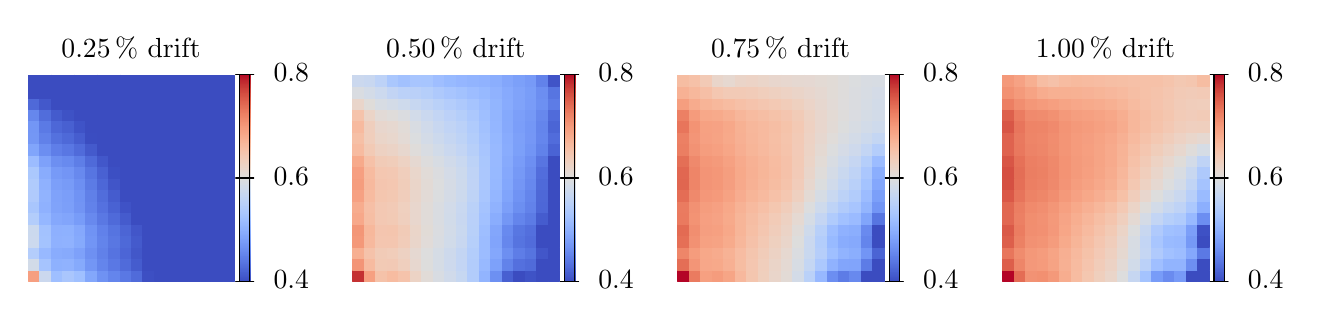
\begin{tikzpicture}[gnuplot]
%% generated with GNUPLOT 5.2p6 (Lua 5.3; terminal rev. Nov 2018, script rev. 107)
%% 03/05/2019 03:06:17
\path (0.000,0.000) rectangle (15.000,3.000);
\gpcolor{color=gp lt color border}
\node[gp node center] at (1.312,3.121) {\SI{0.25}{\percent} drift};
\gpfill{rgb color={0.963,0.625,0.504}} (0.000,0.188)--(0.000,0.334)--(0.146,0.334)--(0.146,0.188)--cycle;
\gpfill{rgb color={0.797,0.849,0.933}} (0.146,0.188)--(0.146,0.334)--(0.292,0.334)--(0.292,0.188)--cycle;
\gpfill{rgb color={0.825,0.858,0.909}} (0.000,0.334)--(0.000,0.480)--(0.146,0.480)--(0.146,0.334)--cycle;
\gpfill{rgb color={0.651,0.768,0.997}} (0.146,0.334)--(0.146,0.480)--(0.292,0.480)--(0.292,0.334)--cycle;
\gpfill{rgb color={0.705,0.804,0.983}} (0.000,0.480)--(0.000,0.626)--(0.146,0.626)--(0.146,0.480)--cycle;
\gpfill{rgb color={0.596,0.726,1.000}} (0.146,0.480)--(0.146,0.626)--(0.292,0.626)--(0.292,0.480)--cycle;
\gpfill{rgb color={0.799,0.850,0.932}} (0.000,0.626)--(0.000,0.771)--(0.146,0.771)--(0.146,0.626)--cycle;
\gpfill{rgb color={0.644,0.763,0.998}} (0.146,0.626)--(0.146,0.771)--(0.292,0.771)--(0.292,0.626)--cycle;
\gpfill{rgb color={0.798,0.850,0.932}} (0.000,0.771)--(0.000,0.917)--(0.146,0.917)--(0.146,0.771)--cycle;
\gpfill{rgb color={0.640,0.760,0.998}} (0.146,0.771)--(0.146,0.917)--(0.292,0.917)--(0.292,0.771)--cycle;
\gpfill{rgb color={0.703,0.803,0.984}} (0.000,0.917)--(0.000,1.063)--(0.146,1.063)--(0.146,0.917)--cycle;
\gpfill{rgb color={0.585,0.717,0.999}} (0.146,0.917)--(0.146,1.063)--(0.292,1.063)--(0.292,0.917)--cycle;
\gpfill{rgb color={0.664,0.777,0.994}} (0.000,1.063)--(0.000,1.209)--(0.146,1.209)--(0.146,1.063)--cycle;
\gpfill{rgb color={0.560,0.696,0.997}} (0.146,1.063)--(0.146,1.209)--(0.292,1.209)--(0.292,1.063)--cycle;
\gpfill{rgb color={0.689,0.794,0.988}} (0.000,1.209)--(0.000,1.355)--(0.146,1.355)--(0.146,1.209)--cycle;
\gpfill{rgb color={0.567,0.701,0.997}} (0.146,1.209)--(0.146,1.355)--(0.292,1.355)--(0.292,1.209)--cycle;
\gpfill{rgb color={0.691,0.795,0.988}} (0.000,1.355)--(0.000,1.500)--(0.146,1.500)--(0.146,1.355)--cycle;
\gpfill{rgb color={0.560,0.695,0.996}} (0.146,1.355)--(0.146,1.500)--(0.292,1.500)--(0.292,1.355)--cycle;
\gpfill{rgb color={0.672,0.783,0.993}} (0.000,1.500)--(0.000,1.645)--(0.146,1.645)--(0.146,1.500)--cycle;
\gpfill{rgb color={0.539,0.676,0.993}} (0.146,1.500)--(0.146,1.645)--(0.292,1.645)--(0.292,1.500)--cycle;
\gpfill{rgb color={0.611,0.738,1.000}} (0.000,1.645)--(0.000,1.791)--(0.146,1.791)--(0.146,1.645)--cycle;
\gpfill{rgb color={0.493,0.632,0.979}} (0.146,1.645)--(0.146,1.791)--(0.292,1.791)--(0.292,1.645)--cycle;
\gpfill{rgb color={0.507,0.646,0.984}} (0.000,1.791)--(0.000,1.937)--(0.146,1.937)--(0.146,1.791)--cycle;
\gpfill{rgb color={0.423,0.557,0.945}} (0.146,1.791)--(0.146,1.937)--(0.292,1.937)--(0.292,1.791)--cycle;
\gpfill{rgb color={0.454,0.591,0.962}} (0.000,1.937)--(0.000,2.083)--(0.146,2.083)--(0.146,1.937)--cycle;
\gpfill{rgb color={0.379,0.504,0.914}} (0.146,1.937)--(0.146,2.083)--(0.292,2.083)--(0.292,1.937)--cycle;
\gpfill{rgb color={0.451,0.587,0.960}} (0.000,2.083)--(0.000,2.229)--(0.146,2.229)--(0.146,2.083)--cycle;
\gpfill{rgb color={0.358,0.478,0.897}} (0.146,2.083)--(0.146,2.229)--(0.292,2.229)--(0.292,2.083)--cycle;
\gpfill{rgb color={0.400,0.530,0.930}} (0.000,2.229)--(0.000,2.374)--(0.146,2.374)--(0.146,2.229)--cycle;
\gpfill{rgb color={0.318,0.426,0.860}} (0.146,2.229)--(0.146,2.374)--(0.292,2.374)--(0.292,2.229)--cycle;
\gpfill{rgb color={0.308,0.412,0.849}} (0.000,2.374)--(0.000,2.520)--(0.146,2.520)--(0.146,2.374)--cycle;
\gpfill{rgb color={0.261,0.345,0.795}} (0.146,2.374)--(0.146,2.520)--(0.292,2.520)--(0.292,2.374)--cycle;
\gpfill{rgb color={0.230,0.299,0.754}} (0.000,2.520)--(0.000,2.666)--(0.146,2.666)--(0.146,2.520)--cycle;
\gpfill{rgb color={0.230,0.299,0.754}} (0.146,2.520)--(0.146,2.666)--(0.292,2.666)--(0.292,2.520)--cycle;
\gpfill{rgb color={0.230,0.299,0.754}} (0.000,2.666)--(0.000,2.812)--(0.146,2.812)--(0.146,2.666)--cycle;
\gpfill{rgb color={0.230,0.299,0.754}} (0.146,2.666)--(0.146,2.812)--(0.292,2.812)--(0.292,2.666)--cycle;
\gpfill{rgb color={0.624,0.748,0.999}} (0.292,0.188)--(0.292,0.334)--(0.438,0.334)--(0.438,0.188)--cycle;
\gpfill{rgb color={0.665,0.778,0.994}} (0.438,0.188)--(0.438,0.334)--(0.583,0.334)--(0.583,0.188)--cycle;
\gpfill{rgb color={0.558,0.693,0.996}} (0.292,0.334)--(0.292,0.480)--(0.438,0.480)--(0.438,0.334)--cycle;
\gpfill{rgb color={0.563,0.698,0.997}} (0.438,0.334)--(0.438,0.480)--(0.583,0.480)--(0.583,0.334)--cycle;
\gpfill{rgb color={0.537,0.674,0.992}} (0.292,0.480)--(0.292,0.626)--(0.438,0.626)--(0.438,0.480)--cycle;
\gpfill{rgb color={0.529,0.667,0.990}} (0.438,0.480)--(0.438,0.626)--(0.583,0.626)--(0.583,0.480)--cycle;
\gpfill{rgb color={0.561,0.696,0.997}} (0.292,0.626)--(0.292,0.771)--(0.438,0.771)--(0.438,0.626)--cycle;
\gpfill{rgb color={0.564,0.699,0.997}} (0.438,0.626)--(0.438,0.771)--(0.583,0.771)--(0.583,0.626)--cycle;
\gpfill{rgb color={0.556,0.691,0.996}} (0.292,0.771)--(0.292,0.917)--(0.438,0.917)--(0.438,0.771)--cycle;
\gpfill{rgb color={0.558,0.693,0.996}} (0.438,0.771)--(0.438,0.917)--(0.583,0.917)--(0.583,0.771)--cycle;
\gpfill{rgb color={0.520,0.658,0.988}} (0.292,0.917)--(0.292,1.063)--(0.438,1.063)--(0.438,0.917)--cycle;
\gpfill{rgb color={0.510,0.649,0.985}} (0.438,0.917)--(0.438,1.063)--(0.583,1.063)--(0.583,0.917)--cycle;
\gpfill{rgb color={0.500,0.639,0.982}} (0.292,1.063)--(0.292,1.209)--(0.438,1.209)--(0.438,1.063)--cycle;
\gpfill{rgb color={0.485,0.624,0.976}} (0.438,1.063)--(0.438,1.209)--(0.583,1.209)--(0.583,1.063)--cycle;
\gpfill{rgb color={0.497,0.636,0.981}} (0.292,1.209)--(0.292,1.355)--(0.438,1.355)--(0.438,1.209)--cycle;
\gpfill{rgb color={0.482,0.620,0.975}} (0.438,1.209)--(0.438,1.355)--(0.583,1.355)--(0.583,1.209)--cycle;
\gpfill{rgb color={0.485,0.624,0.976}} (0.292,1.355)--(0.292,1.500)--(0.438,1.500)--(0.438,1.355)--cycle;
\gpfill{rgb color={0.470,0.608,0.970}} (0.438,1.355)--(0.438,1.500)--(0.583,1.500)--(0.583,1.355)--cycle;
\gpfill{rgb color={0.465,0.603,0.967}} (0.292,1.500)--(0.292,1.645)--(0.438,1.645)--(0.438,1.500)--cycle;
\gpfill{rgb color={0.450,0.586,0.960}} (0.438,1.500)--(0.438,1.645)--(0.583,1.645)--(0.583,1.500)--cycle;
\gpfill{rgb color={0.426,0.560,0.947}} (0.292,1.645)--(0.292,1.791)--(0.438,1.791)--(0.438,1.645)--cycle;
\gpfill{rgb color={0.409,0.540,0.936}} (0.438,1.645)--(0.438,1.791)--(0.583,1.791)--(0.583,1.645)--cycle;
\gpfill{rgb color={0.371,0.495,0.908}} (0.292,1.791)--(0.292,1.937)--(0.438,1.937)--(0.438,1.791)--cycle;
\gpfill{rgb color={0.350,0.467,0.890}} (0.438,1.791)--(0.438,1.937)--(0.583,1.937)--(0.583,1.791)--cycle;
\gpfill{rgb color={0.330,0.443,0.872}} (0.292,1.937)--(0.292,2.083)--(0.438,2.083)--(0.438,1.937)--cycle;
\gpfill{rgb color={0.307,0.411,0.849}} (0.438,1.937)--(0.438,2.083)--(0.583,2.083)--(0.583,1.937)--cycle;
\gpfill{rgb color={0.303,0.405,0.844}} (0.292,2.083)--(0.292,2.229)--(0.438,2.229)--(0.438,2.083)--cycle;
\gpfill{rgb color={0.281,0.375,0.819}} (0.438,2.083)--(0.438,2.229)--(0.583,2.229)--(0.583,2.083)--cycle;
\gpfill{rgb color={0.267,0.355,0.803}} (0.292,2.229)--(0.292,2.374)--(0.438,2.374)--(0.438,2.229)--cycle;
\gpfill{rgb color={0.245,0.321,0.774}} (0.438,2.229)--(0.438,2.374)--(0.583,2.374)--(0.583,2.229)--cycle;
\gpfill{rgb color={0.230,0.299,0.754}} (0.292,2.374)--(0.292,2.520)--(0.438,2.520)--(0.438,2.374)--cycle;
\gpfill{rgb color={0.230,0.299,0.754}} (0.438,2.374)--(0.438,2.520)--(0.583,2.520)--(0.583,2.374)--cycle;
\gpfill{rgb color={0.230,0.299,0.754}} (0.292,2.520)--(0.292,2.666)--(0.438,2.666)--(0.438,2.520)--cycle;
\gpfill{rgb color={0.230,0.299,0.754}} (0.438,2.520)--(0.438,2.666)--(0.583,2.666)--(0.583,2.520)--cycle;
\gpfill{rgb color={0.230,0.299,0.754}} (0.292,2.666)--(0.292,2.812)--(0.438,2.812)--(0.438,2.666)--cycle;
\gpfill{rgb color={0.230,0.299,0.754}} (0.438,2.666)--(0.438,2.812)--(0.583,2.812)--(0.583,2.666)--cycle;
\gpfill{rgb color={0.629,0.752,0.999}} (0.583,0.188)--(0.583,0.334)--(0.729,0.334)--(0.729,0.188)--cycle;
\gpfill{rgb color={0.514,0.653,0.986}} (0.729,0.188)--(0.729,0.334)--(0.875,0.334)--(0.875,0.188)--cycle;
\gpfill{rgb color={0.527,0.665,0.990}} (0.583,0.334)--(0.583,0.480)--(0.729,0.480)--(0.729,0.334)--cycle;
\gpfill{rgb color={0.452,0.588,0.961}} (0.729,0.334)--(0.729,0.480)--(0.875,0.480)--(0.875,0.334)--cycle;
\gpfill{rgb color={0.493,0.632,0.979}} (0.583,0.480)--(0.583,0.626)--(0.729,0.626)--(0.729,0.480)--cycle;
\gpfill{rgb color={0.430,0.565,0.949}} (0.729,0.480)--(0.729,0.626)--(0.875,0.626)--(0.875,0.480)--cycle;
\gpfill{rgb color={0.527,0.665,0.990}} (0.583,0.626)--(0.583,0.771)--(0.729,0.771)--(0.729,0.626)--cycle;
\gpfill{rgb color={0.449,0.586,0.960}} (0.729,0.626)--(0.729,0.771)--(0.875,0.771)--(0.875,0.626)--cycle;
\gpfill{rgb color={0.520,0.658,0.988}} (0.583,0.771)--(0.583,0.917)--(0.729,0.917)--(0.729,0.771)--cycle;
\gpfill{rgb color={0.441,0.577,0.955}} (0.729,0.771)--(0.729,0.917)--(0.875,0.917)--(0.875,0.771)--cycle;
\gpfill{rgb color={0.472,0.610,0.971}} (0.583,0.917)--(0.583,1.063)--(0.729,1.063)--(0.729,0.917)--cycle;
\gpfill{rgb color={0.406,0.537,0.934}} (0.729,0.917)--(0.729,1.063)--(0.875,1.063)--(0.875,0.917)--cycle;
\gpfill{rgb color={0.446,0.582,0.958}} (0.583,1.063)--(0.583,1.209)--(0.729,1.209)--(0.729,1.063)--cycle;
\gpfill{rgb color={0.385,0.511,0.919}} (0.729,1.063)--(0.729,1.209)--(0.875,1.209)--(0.875,1.063)--cycle;
\gpfill{rgb color={0.440,0.576,0.955}} (0.583,1.209)--(0.583,1.355)--(0.729,1.355)--(0.729,1.209)--cycle;
\gpfill{rgb color={0.375,0.500,0.911}} (0.729,1.209)--(0.729,1.355)--(0.875,1.355)--(0.875,1.209)--cycle;
\gpfill{rgb color={0.428,0.562,0.948}} (0.583,1.355)--(0.583,1.500)--(0.729,1.500)--(0.729,1.355)--cycle;
\gpfill{rgb color={0.361,0.482,0.900}} (0.729,1.355)--(0.729,1.500)--(0.875,1.500)--(0.875,1.355)--cycle;
\gpfill{rgb color={0.408,0.539,0.935}} (0.583,1.500)--(0.583,1.645)--(0.729,1.645)--(0.729,1.500)--cycle;
\gpfill{rgb color={0.342,0.458,0.883}} (0.729,1.500)--(0.729,1.645)--(0.875,1.645)--(0.875,1.500)--cycle;
\gpfill{rgb color={0.370,0.493,0.907}} (0.583,1.645)--(0.583,1.791)--(0.729,1.791)--(0.729,1.645)--cycle;
\gpfill{rgb color={0.310,0.416,0.852}} (0.729,1.645)--(0.729,1.791)--(0.875,1.791)--(0.875,1.645)--cycle;
\gpfill{rgb color={0.314,0.420,0.856}} (0.583,1.791)--(0.583,1.937)--(0.729,1.937)--(0.729,1.791)--cycle;
\gpfill{rgb color={0.266,0.353,0.801}} (0.729,1.791)--(0.729,1.937)--(0.875,1.937)--(0.875,1.791)--cycle;
\gpfill{rgb color={0.274,0.365,0.811}} (0.583,1.937)--(0.583,2.083)--(0.729,2.083)--(0.729,1.937)--cycle;
\gpfill{rgb color={0.232,0.302,0.756}} (0.729,1.937)--(0.729,2.083)--(0.875,2.083)--(0.875,1.937)--cycle;
\gpfill{rgb color={0.249,0.327,0.779}} (0.583,2.083)--(0.583,2.229)--(0.729,2.229)--(0.729,2.083)--cycle;
\gpfill{rgb color={0.230,0.299,0.754}} (0.729,2.083)--(0.729,2.229)--(0.875,2.229)--(0.875,2.083)--cycle;
\gpfill{rgb color={0.230,0.299,0.754}} (0.583,2.229)--(0.583,2.374)--(0.729,2.374)--(0.729,2.229)--cycle;
\gpfill{rgb color={0.230,0.299,0.754}} (0.729,2.229)--(0.729,2.374)--(0.875,2.374)--(0.875,2.229)--cycle;
\gpfill{rgb color={0.230,0.299,0.754}} (0.583,2.374)--(0.583,2.520)--(0.729,2.520)--(0.729,2.374)--cycle;
\gpfill{rgb color={0.230,0.299,0.754}} (0.729,2.374)--(0.729,2.520)--(0.875,2.520)--(0.875,2.374)--cycle;
\gpfill{rgb color={0.230,0.299,0.754}} (0.583,2.520)--(0.583,2.666)--(0.729,2.666)--(0.729,2.520)--cycle;
\gpfill{rgb color={0.230,0.299,0.754}} (0.729,2.520)--(0.729,2.666)--(0.875,2.666)--(0.875,2.520)--cycle;
\gpfill{rgb color={0.230,0.299,0.754}} (0.583,2.666)--(0.583,2.812)--(0.729,2.812)--(0.729,2.666)--cycle;
\gpfill{rgb color={0.230,0.299,0.754}} (0.729,2.666)--(0.729,2.812)--(0.875,2.812)--(0.875,2.666)--cycle;
\gpfill{rgb color={0.436,0.571,0.952}} (0.875,0.188)--(0.875,0.334)--(1.021,0.334)--(1.021,0.188)--cycle;
\gpfill{rgb color={0.394,0.523,0.926}} (1.021,0.188)--(1.021,0.334)--(1.167,0.334)--(1.167,0.188)--cycle;
\gpfill{rgb color={0.394,0.522,0.925}} (0.875,0.334)--(0.875,0.480)--(1.021,0.480)--(1.021,0.334)--cycle;
\gpfill{rgb color={0.353,0.472,0.893}} (1.021,0.334)--(1.021,0.480)--(1.167,0.480)--(1.167,0.334)--cycle;
\gpfill{rgb color={0.379,0.504,0.914}} (0.875,0.480)--(0.875,0.626)--(1.021,0.626)--(1.021,0.480)--cycle;
\gpfill{rgb color={0.338,0.452,0.879}} (1.021,0.480)--(1.021,0.626)--(1.167,0.626)--(1.167,0.480)--cycle;
\gpfill{rgb color={0.390,0.518,0.923}} (0.875,0.626)--(0.875,0.771)--(1.021,0.771)--(1.021,0.626)--cycle;
\gpfill{rgb color={0.348,0.465,0.888}} (1.021,0.626)--(1.021,0.771)--(1.167,0.771)--(1.167,0.626)--cycle;
\gpfill{rgb color={0.381,0.507,0.916}} (0.875,0.771)--(0.875,0.917)--(1.021,0.917)--(1.021,0.771)--cycle;
\gpfill{rgb color={0.338,0.453,0.880}} (1.021,0.771)--(1.021,0.917)--(1.167,0.917)--(1.167,0.771)--cycle;
\gpfill{rgb color={0.353,0.471,0.892}} (0.875,0.917)--(0.875,1.063)--(1.021,1.063)--(1.021,0.917)--cycle;
\gpfill{rgb color={0.310,0.414,0.851}} (1.021,0.917)--(1.021,1.063)--(1.167,1.063)--(1.167,0.917)--cycle;
\gpfill{rgb color={0.332,0.444,0.873}} (0.875,1.063)--(0.875,1.209)--(1.021,1.209)--(1.021,1.063)--cycle;
\gpfill{rgb color={0.287,0.383,0.826}} (1.021,1.063)--(1.021,1.209)--(1.167,1.209)--(1.167,1.063)--cycle;
\gpfill{rgb color={0.318,0.426,0.860}} (0.875,1.209)--(0.875,1.355)--(1.021,1.355)--(1.021,1.209)--cycle;
\gpfill{rgb color={0.270,0.359,0.806}} (1.021,1.209)--(1.021,1.355)--(1.167,1.355)--(1.167,1.209)--cycle;
\gpfill{rgb color={0.303,0.405,0.844}} (0.875,1.355)--(0.875,1.500)--(1.021,1.500)--(1.021,1.355)--cycle;
\gpfill{rgb color={0.253,0.334,0.785}} (1.021,1.355)--(1.021,1.500)--(1.167,1.500)--(1.167,1.355)--cycle;
\gpfill{rgb color={0.286,0.381,0.825}} (0.875,1.500)--(0.875,1.645)--(1.021,1.645)--(1.021,1.500)--cycle;
\gpfill{rgb color={0.237,0.310,0.764}} (1.021,1.500)--(1.021,1.645)--(1.167,1.645)--(1.167,1.500)--cycle;
\gpfill{rgb color={0.258,0.341,0.791}} (0.875,1.645)--(0.875,1.791)--(1.021,1.791)--(1.021,1.645)--cycle;
\gpfill{rgb color={0.230,0.299,0.754}} (1.021,1.645)--(1.021,1.791)--(1.167,1.791)--(1.167,1.645)--cycle;
\gpfill{rgb color={0.230,0.299,0.754}} (0.875,1.791)--(0.875,1.937)--(1.021,1.937)--(1.021,1.791)--cycle;
\gpfill{rgb color={0.230,0.299,0.754}} (1.021,1.791)--(1.021,1.937)--(1.167,1.937)--(1.167,1.791)--cycle;
\gpfill{rgb color={0.230,0.299,0.754}} (0.875,1.937)--(0.875,2.083)--(1.021,2.083)--(1.021,1.937)--cycle;
\gpfill{rgb color={0.230,0.299,0.754}} (1.021,1.937)--(1.021,2.083)--(1.167,2.083)--(1.167,1.937)--cycle;
\gpfill{rgb color={0.230,0.299,0.754}} (0.875,2.083)--(0.875,2.229)--(1.021,2.229)--(1.021,2.083)--cycle;
\gpfill{rgb color={0.230,0.299,0.754}} (1.021,2.083)--(1.021,2.229)--(1.167,2.229)--(1.167,2.083)--cycle;
\gpfill{rgb color={0.230,0.299,0.754}} (0.875,2.229)--(0.875,2.374)--(1.021,2.374)--(1.021,2.229)--cycle;
\gpfill{rgb color={0.230,0.299,0.754}} (1.021,2.229)--(1.021,2.374)--(1.167,2.374)--(1.167,2.229)--cycle;
\gpfill{rgb color={0.230,0.299,0.754}} (0.875,2.374)--(0.875,2.520)--(1.021,2.520)--(1.021,2.374)--cycle;
\gpfill{rgb color={0.230,0.299,0.754}} (1.021,2.374)--(1.021,2.520)--(1.167,2.520)--(1.167,2.374)--cycle;
\gpfill{rgb color={0.230,0.299,0.754}} (0.875,2.520)--(0.875,2.666)--(1.021,2.666)--(1.021,2.520)--cycle;
\gpfill{rgb color={0.230,0.299,0.754}} (1.021,2.520)--(1.021,2.666)--(1.167,2.666)--(1.167,2.520)--cycle;
\gpfill{rgb color={0.230,0.299,0.754}} (0.875,2.666)--(0.875,2.812)--(1.021,2.812)--(1.021,2.666)--cycle;
\gpfill{rgb color={0.230,0.299,0.754}} (1.021,2.666)--(1.021,2.812)--(1.167,2.812)--(1.167,2.666)--cycle;
\gpfill{rgb color={0.353,0.472,0.893}} (1.167,0.188)--(1.167,0.334)--(1.312,0.334)--(1.312,0.188)--cycle;
\gpfill{rgb color={0.313,0.418,0.854}} (1.312,0.188)--(1.312,0.334)--(1.457,0.334)--(1.457,0.188)--cycle;
\gpfill{rgb color={0.312,0.418,0.854}} (1.167,0.334)--(1.167,0.480)--(1.312,0.480)--(1.312,0.334)--cycle;
\gpfill{rgb color={0.272,0.362,0.809}} (1.312,0.334)--(1.312,0.480)--(1.457,0.480)--(1.457,0.334)--cycle;
\gpfill{rgb color={0.297,0.397,0.838}} (1.167,0.480)--(1.167,0.626)--(1.312,0.626)--(1.312,0.480)--cycle;
\gpfill{rgb color={0.257,0.340,0.790}} (1.312,0.480)--(1.312,0.626)--(1.457,0.626)--(1.457,0.480)--cycle;
\gpfill{rgb color={0.306,0.410,0.848}} (1.167,0.626)--(1.167,0.771)--(1.312,0.771)--(1.312,0.626)--cycle;
\gpfill{rgb color={0.266,0.353,0.801}} (1.312,0.626)--(1.312,0.771)--(1.457,0.771)--(1.457,0.626)--cycle;
\gpfill{rgb color={0.297,0.397,0.837}} (1.167,0.771)--(1.167,0.917)--(1.312,0.917)--(1.312,0.771)--cycle;
\gpfill{rgb color={0.257,0.339,0.790}} (1.312,0.771)--(1.312,0.917)--(1.457,0.917)--(1.457,0.771)--cycle;
\gpfill{rgb color={0.269,0.357,0.805}} (1.167,0.917)--(1.167,1.063)--(1.312,1.063)--(1.312,0.917)--cycle;
\gpfill{rgb color={0.230,0.299,0.754}} (1.312,0.917)--(1.312,1.063)--(1.457,1.063)--(1.457,0.917)--cycle;
\gpfill{rgb color={0.246,0.323,0.776}} (1.167,1.063)--(1.167,1.209)--(1.312,1.209)--(1.312,1.063)--cycle;
\gpfill{rgb color={0.230,0.299,0.754}} (1.312,1.063)--(1.312,1.209)--(1.457,1.209)--(1.457,1.063)--cycle;
\gpfill{rgb color={0.230,0.299,0.754}} (1.167,1.209)--(1.167,1.355)--(1.312,1.355)--(1.312,1.209)--cycle;
\gpfill{rgb color={0.230,0.299,0.754}} (1.312,1.209)--(1.312,1.355)--(1.457,1.355)--(1.457,1.209)--cycle;
\gpfill{rgb color={0.230,0.299,0.754}} (1.167,1.355)--(1.167,1.500)--(1.312,1.500)--(1.312,1.355)--cycle;
\gpfill{rgb color={0.230,0.299,0.754}} (1.312,1.355)--(1.312,1.500)--(1.457,1.500)--(1.457,1.355)--cycle;
\gpfill{rgb color={0.230,0.299,0.754}} (1.167,1.500)--(1.167,1.645)--(1.312,1.645)--(1.312,1.500)--cycle;
\gpfill{rgb color={0.230,0.299,0.754}} (1.312,1.500)--(1.312,1.645)--(1.457,1.645)--(1.457,1.500)--cycle;
\gpfill{rgb color={0.230,0.299,0.754}} (1.167,1.645)--(1.167,1.791)--(1.312,1.791)--(1.312,1.645)--cycle;
\gpfill{rgb color={0.230,0.299,0.754}} (1.312,1.645)--(1.312,1.791)--(1.457,1.791)--(1.457,1.645)--cycle;
\gpfill{rgb color={0.230,0.299,0.754}} (1.167,1.791)--(1.167,1.937)--(1.312,1.937)--(1.312,1.791)--cycle;
\gpfill{rgb color={0.230,0.299,0.754}} (1.312,1.791)--(1.312,1.937)--(1.457,1.937)--(1.457,1.791)--cycle;
\gpfill{rgb color={0.230,0.299,0.754}} (1.167,1.937)--(1.167,2.083)--(1.312,2.083)--(1.312,1.937)--cycle;
\gpfill{rgb color={0.230,0.299,0.754}} (1.312,1.937)--(1.312,2.083)--(1.457,2.083)--(1.457,1.937)--cycle;
\gpfill{rgb color={0.230,0.299,0.754}} (1.167,2.083)--(1.167,2.229)--(1.312,2.229)--(1.312,2.083)--cycle;
\gpfill{rgb color={0.230,0.299,0.754}} (1.312,2.083)--(1.312,2.229)--(1.457,2.229)--(1.457,2.083)--cycle;
\gpfill{rgb color={0.230,0.299,0.754}} (1.167,2.229)--(1.167,2.374)--(1.312,2.374)--(1.312,2.229)--cycle;
\gpfill{rgb color={0.230,0.299,0.754}} (1.312,2.229)--(1.312,2.374)--(1.457,2.374)--(1.457,2.229)--cycle;
\gpfill{rgb color={0.230,0.299,0.754}} (1.167,2.374)--(1.167,2.520)--(1.312,2.520)--(1.312,2.374)--cycle;
\gpfill{rgb color={0.230,0.299,0.754}} (1.312,2.374)--(1.312,2.520)--(1.457,2.520)--(1.457,2.374)--cycle;
\gpfill{rgb color={0.230,0.299,0.754}} (1.167,2.520)--(1.167,2.666)--(1.312,2.666)--(1.312,2.520)--cycle;
\gpfill{rgb color={0.230,0.299,0.754}} (1.312,2.520)--(1.312,2.666)--(1.457,2.666)--(1.457,2.520)--cycle;
\gpfill{rgb color={0.230,0.299,0.754}} (1.167,2.666)--(1.167,2.812)--(1.312,2.812)--(1.312,2.666)--cycle;
\gpfill{rgb color={0.230,0.299,0.754}} (1.312,2.666)--(1.312,2.812)--(1.457,2.812)--(1.457,2.666)--cycle;
\gpfill{rgb color={0.238,0.311,0.764}} (1.457,0.188)--(1.457,0.334)--(1.603,0.334)--(1.603,0.188)--cycle;
\gpfill{rgb color={0.230,0.299,0.754}} (1.603,0.188)--(1.603,0.334)--(1.749,0.334)--(1.749,0.188)--cycle;
\gpfill{rgb color={0.230,0.299,0.754}} (1.457,0.334)--(1.457,0.480)--(1.603,0.480)--(1.603,0.334)--cycle;
\gpfill{rgb color={0.230,0.299,0.754}} (1.603,0.334)--(1.603,0.480)--(1.749,0.480)--(1.749,0.334)--cycle;
\gpfill{rgb color={0.230,0.299,0.754}} (1.457,0.480)--(1.457,0.626)--(1.603,0.626)--(1.603,0.480)--cycle;
\gpfill{rgb color={0.230,0.299,0.754}} (1.603,0.480)--(1.603,0.626)--(1.749,0.626)--(1.749,0.480)--cycle;
\gpfill{rgb color={0.230,0.299,0.754}} (1.457,0.626)--(1.457,0.771)--(1.603,0.771)--(1.603,0.626)--cycle;
\gpfill{rgb color={0.230,0.299,0.754}} (1.603,0.626)--(1.603,0.771)--(1.749,0.771)--(1.749,0.626)--cycle;
\gpfill{rgb color={0.230,0.299,0.754}} (1.457,0.771)--(1.457,0.917)--(1.603,0.917)--(1.603,0.771)--cycle;
\gpfill{rgb color={0.230,0.299,0.754}} (1.603,0.771)--(1.603,0.917)--(1.749,0.917)--(1.749,0.771)--cycle;
\gpfill{rgb color={0.230,0.299,0.754}} (1.457,0.917)--(1.457,1.063)--(1.603,1.063)--(1.603,0.917)--cycle;
\gpfill{rgb color={0.230,0.299,0.754}} (1.603,0.917)--(1.603,1.063)--(1.749,1.063)--(1.749,0.917)--cycle;
\gpfill{rgb color={0.230,0.299,0.754}} (1.457,1.063)--(1.457,1.209)--(1.603,1.209)--(1.603,1.063)--cycle;
\gpfill{rgb color={0.230,0.299,0.754}} (1.603,1.063)--(1.603,1.209)--(1.749,1.209)--(1.749,1.063)--cycle;
\gpfill{rgb color={0.230,0.299,0.754}} (1.457,1.209)--(1.457,1.355)--(1.603,1.355)--(1.603,1.209)--cycle;
\gpfill{rgb color={0.230,0.299,0.754}} (1.603,1.209)--(1.603,1.355)--(1.749,1.355)--(1.749,1.209)--cycle;
\gpfill{rgb color={0.230,0.299,0.754}} (1.457,1.355)--(1.457,1.500)--(1.603,1.500)--(1.603,1.355)--cycle;
\gpfill{rgb color={0.230,0.299,0.754}} (1.603,1.355)--(1.603,1.500)--(1.749,1.500)--(1.749,1.355)--cycle;
\gpfill{rgb color={0.230,0.299,0.754}} (1.457,1.500)--(1.457,1.645)--(1.603,1.645)--(1.603,1.500)--cycle;
\gpfill{rgb color={0.230,0.299,0.754}} (1.603,1.500)--(1.603,1.645)--(1.749,1.645)--(1.749,1.500)--cycle;
\gpfill{rgb color={0.230,0.299,0.754}} (1.457,1.645)--(1.457,1.791)--(1.603,1.791)--(1.603,1.645)--cycle;
\gpfill{rgb color={0.230,0.299,0.754}} (1.603,1.645)--(1.603,1.791)--(1.749,1.791)--(1.749,1.645)--cycle;
\gpfill{rgb color={0.230,0.299,0.754}} (1.457,1.791)--(1.457,1.937)--(1.603,1.937)--(1.603,1.791)--cycle;
\gpfill{rgb color={0.230,0.299,0.754}} (1.603,1.791)--(1.603,1.937)--(1.749,1.937)--(1.749,1.791)--cycle;
\gpfill{rgb color={0.230,0.299,0.754}} (1.457,1.937)--(1.457,2.083)--(1.603,2.083)--(1.603,1.937)--cycle;
\gpfill{rgb color={0.230,0.299,0.754}} (1.603,1.937)--(1.603,2.083)--(1.749,2.083)--(1.749,1.937)--cycle;
\gpfill{rgb color={0.230,0.299,0.754}} (1.457,2.083)--(1.457,2.229)--(1.603,2.229)--(1.603,2.083)--cycle;
\gpfill{rgb color={0.230,0.299,0.754}} (1.603,2.083)--(1.603,2.229)--(1.749,2.229)--(1.749,2.083)--cycle;
\gpfill{rgb color={0.230,0.299,0.754}} (1.457,2.229)--(1.457,2.374)--(1.603,2.374)--(1.603,2.229)--cycle;
\gpfill{rgb color={0.230,0.299,0.754}} (1.603,2.229)--(1.603,2.374)--(1.749,2.374)--(1.749,2.229)--cycle;
\gpfill{rgb color={0.230,0.299,0.754}} (1.457,2.374)--(1.457,2.520)--(1.603,2.520)--(1.603,2.374)--cycle;
\gpfill{rgb color={0.230,0.299,0.754}} (1.603,2.374)--(1.603,2.520)--(1.749,2.520)--(1.749,2.374)--cycle;
\gpfill{rgb color={0.230,0.299,0.754}} (1.457,2.520)--(1.457,2.666)--(1.603,2.666)--(1.603,2.520)--cycle;
\gpfill{rgb color={0.230,0.299,0.754}} (1.603,2.520)--(1.603,2.666)--(1.749,2.666)--(1.749,2.520)--cycle;
\gpfill{rgb color={0.230,0.299,0.754}} (1.457,2.666)--(1.457,2.812)--(1.603,2.812)--(1.603,2.666)--cycle;
\gpfill{rgb color={0.230,0.299,0.754}} (1.603,2.666)--(1.603,2.812)--(1.749,2.812)--(1.749,2.666)--cycle;
\gpfill{rgb color={0.230,0.299,0.754}} (1.749,0.188)--(1.749,0.334)--(1.895,0.334)--(1.895,0.188)--cycle;
\gpfill{rgb color={0.230,0.299,0.754}} (1.895,0.188)--(1.895,0.334)--(2.041,0.334)--(2.041,0.188)--cycle;
\gpfill{rgb color={0.230,0.299,0.754}} (1.749,0.334)--(1.749,0.480)--(1.895,0.480)--(1.895,0.334)--cycle;
\gpfill{rgb color={0.230,0.299,0.754}} (1.895,0.334)--(1.895,0.480)--(2.041,0.480)--(2.041,0.334)--cycle;
\gpfill{rgb color={0.230,0.299,0.754}} (1.749,0.480)--(1.749,0.626)--(1.895,0.626)--(1.895,0.480)--cycle;
\gpfill{rgb color={0.230,0.299,0.754}} (1.895,0.480)--(1.895,0.626)--(2.041,0.626)--(2.041,0.480)--cycle;
\gpfill{rgb color={0.230,0.299,0.754}} (1.749,0.626)--(1.749,0.771)--(1.895,0.771)--(1.895,0.626)--cycle;
\gpfill{rgb color={0.230,0.299,0.754}} (1.895,0.626)--(1.895,0.771)--(2.041,0.771)--(2.041,0.626)--cycle;
\gpfill{rgb color={0.230,0.299,0.754}} (1.749,0.771)--(1.749,0.917)--(1.895,0.917)--(1.895,0.771)--cycle;
\gpfill{rgb color={0.230,0.299,0.754}} (1.895,0.771)--(1.895,0.917)--(2.041,0.917)--(2.041,0.771)--cycle;
\gpfill{rgb color={0.230,0.299,0.754}} (1.749,0.917)--(1.749,1.063)--(1.895,1.063)--(1.895,0.917)--cycle;
\gpfill{rgb color={0.230,0.299,0.754}} (1.895,0.917)--(1.895,1.063)--(2.041,1.063)--(2.041,0.917)--cycle;
\gpfill{rgb color={0.230,0.299,0.754}} (1.749,1.063)--(1.749,1.209)--(1.895,1.209)--(1.895,1.063)--cycle;
\gpfill{rgb color={0.230,0.299,0.754}} (1.895,1.063)--(1.895,1.209)--(2.041,1.209)--(2.041,1.063)--cycle;
\gpfill{rgb color={0.230,0.299,0.754}} (1.749,1.209)--(1.749,1.355)--(1.895,1.355)--(1.895,1.209)--cycle;
\gpfill{rgb color={0.230,0.299,0.754}} (1.895,1.209)--(1.895,1.355)--(2.041,1.355)--(2.041,1.209)--cycle;
\gpfill{rgb color={0.230,0.299,0.754}} (1.749,1.355)--(1.749,1.500)--(1.895,1.500)--(1.895,1.355)--cycle;
\gpfill{rgb color={0.230,0.299,0.754}} (1.895,1.355)--(1.895,1.500)--(2.041,1.500)--(2.041,1.355)--cycle;
\gpfill{rgb color={0.230,0.299,0.754}} (1.749,1.500)--(1.749,1.645)--(1.895,1.645)--(1.895,1.500)--cycle;
\gpfill{rgb color={0.230,0.299,0.754}} (1.895,1.500)--(1.895,1.645)--(2.041,1.645)--(2.041,1.500)--cycle;
\gpfill{rgb color={0.230,0.299,0.754}} (1.749,1.645)--(1.749,1.791)--(1.895,1.791)--(1.895,1.645)--cycle;
\gpfill{rgb color={0.230,0.299,0.754}} (1.895,1.645)--(1.895,1.791)--(2.041,1.791)--(2.041,1.645)--cycle;
\gpfill{rgb color={0.230,0.299,0.754}} (1.749,1.791)--(1.749,1.937)--(1.895,1.937)--(1.895,1.791)--cycle;
\gpfill{rgb color={0.230,0.299,0.754}} (1.895,1.791)--(1.895,1.937)--(2.041,1.937)--(2.041,1.791)--cycle;
\gpfill{rgb color={0.230,0.299,0.754}} (1.749,1.937)--(1.749,2.083)--(1.895,2.083)--(1.895,1.937)--cycle;
\gpfill{rgb color={0.230,0.299,0.754}} (1.895,1.937)--(1.895,2.083)--(2.041,2.083)--(2.041,1.937)--cycle;
\gpfill{rgb color={0.230,0.299,0.754}} (1.749,2.083)--(1.749,2.229)--(1.895,2.229)--(1.895,2.083)--cycle;
\gpfill{rgb color={0.230,0.299,0.754}} (1.895,2.083)--(1.895,2.229)--(2.041,2.229)--(2.041,2.083)--cycle;
\gpfill{rgb color={0.230,0.299,0.754}} (1.749,2.229)--(1.749,2.374)--(1.895,2.374)--(1.895,2.229)--cycle;
\gpfill{rgb color={0.230,0.299,0.754}} (1.895,2.229)--(1.895,2.374)--(2.041,2.374)--(2.041,2.229)--cycle;
\gpfill{rgb color={0.230,0.299,0.754}} (1.749,2.374)--(1.749,2.520)--(1.895,2.520)--(1.895,2.374)--cycle;
\gpfill{rgb color={0.230,0.299,0.754}} (1.895,2.374)--(1.895,2.520)--(2.041,2.520)--(2.041,2.374)--cycle;
\gpfill{rgb color={0.230,0.299,0.754}} (1.749,2.520)--(1.749,2.666)--(1.895,2.666)--(1.895,2.520)--cycle;
\gpfill{rgb color={0.230,0.299,0.754}} (1.895,2.520)--(1.895,2.666)--(2.041,2.666)--(2.041,2.520)--cycle;
\gpfill{rgb color={0.230,0.299,0.754}} (1.749,2.666)--(1.749,2.812)--(1.895,2.812)--(1.895,2.666)--cycle;
\gpfill{rgb color={0.230,0.299,0.754}} (1.895,2.666)--(1.895,2.812)--(2.041,2.812)--(2.041,2.666)--cycle;
\gpfill{rgb color={0.230,0.299,0.754}} (2.041,0.188)--(2.041,0.334)--(2.186,0.334)--(2.186,0.188)--cycle;
\gpfill{rgb color={0.230,0.299,0.754}} (2.186,0.188)--(2.186,0.334)--(2.332,0.334)--(2.332,0.188)--cycle;
\gpfill{rgb color={0.230,0.299,0.754}} (2.041,0.334)--(2.041,0.480)--(2.186,0.480)--(2.186,0.334)--cycle;
\gpfill{rgb color={0.230,0.299,0.754}} (2.186,0.334)--(2.186,0.480)--(2.332,0.480)--(2.332,0.334)--cycle;
\gpfill{rgb color={0.230,0.299,0.754}} (2.041,0.480)--(2.041,0.626)--(2.186,0.626)--(2.186,0.480)--cycle;
\gpfill{rgb color={0.230,0.299,0.754}} (2.186,0.480)--(2.186,0.626)--(2.332,0.626)--(2.332,0.480)--cycle;
\gpfill{rgb color={0.230,0.299,0.754}} (2.041,0.626)--(2.041,0.771)--(2.186,0.771)--(2.186,0.626)--cycle;
\gpfill{rgb color={0.230,0.299,0.754}} (2.186,0.626)--(2.186,0.771)--(2.332,0.771)--(2.332,0.626)--cycle;
\gpfill{rgb color={0.230,0.299,0.754}} (2.041,0.771)--(2.041,0.917)--(2.186,0.917)--(2.186,0.771)--cycle;
\gpfill{rgb color={0.230,0.299,0.754}} (2.186,0.771)--(2.186,0.917)--(2.332,0.917)--(2.332,0.771)--cycle;
\gpfill{rgb color={0.230,0.299,0.754}} (2.041,0.917)--(2.041,1.063)--(2.186,1.063)--(2.186,0.917)--cycle;
\gpfill{rgb color={0.230,0.299,0.754}} (2.186,0.917)--(2.186,1.063)--(2.332,1.063)--(2.332,0.917)--cycle;
\gpfill{rgb color={0.230,0.299,0.754}} (2.041,1.063)--(2.041,1.209)--(2.186,1.209)--(2.186,1.063)--cycle;
\gpfill{rgb color={0.230,0.299,0.754}} (2.186,1.063)--(2.186,1.209)--(2.332,1.209)--(2.332,1.063)--cycle;
\gpfill{rgb color={0.230,0.299,0.754}} (2.041,1.209)--(2.041,1.355)--(2.186,1.355)--(2.186,1.209)--cycle;
\gpfill{rgb color={0.230,0.299,0.754}} (2.186,1.209)--(2.186,1.355)--(2.332,1.355)--(2.332,1.209)--cycle;
\gpfill{rgb color={0.230,0.299,0.754}} (2.041,1.355)--(2.041,1.500)--(2.186,1.500)--(2.186,1.355)--cycle;
\gpfill{rgb color={0.230,0.299,0.754}} (2.186,1.355)--(2.186,1.500)--(2.332,1.500)--(2.332,1.355)--cycle;
\gpfill{rgb color={0.230,0.299,0.754}} (2.041,1.500)--(2.041,1.645)--(2.186,1.645)--(2.186,1.500)--cycle;
\gpfill{rgb color={0.230,0.299,0.754}} (2.186,1.500)--(2.186,1.645)--(2.332,1.645)--(2.332,1.500)--cycle;
\gpfill{rgb color={0.230,0.299,0.754}} (2.041,1.645)--(2.041,1.791)--(2.186,1.791)--(2.186,1.645)--cycle;
\gpfill{rgb color={0.230,0.299,0.754}} (2.186,1.645)--(2.186,1.791)--(2.332,1.791)--(2.332,1.645)--cycle;
\gpfill{rgb color={0.230,0.299,0.754}} (2.041,1.791)--(2.041,1.937)--(2.186,1.937)--(2.186,1.791)--cycle;
\gpfill{rgb color={0.230,0.299,0.754}} (2.186,1.791)--(2.186,1.937)--(2.332,1.937)--(2.332,1.791)--cycle;
\gpfill{rgb color={0.230,0.299,0.754}} (2.041,1.937)--(2.041,2.083)--(2.186,2.083)--(2.186,1.937)--cycle;
\gpfill{rgb color={0.230,0.299,0.754}} (2.186,1.937)--(2.186,2.083)--(2.332,2.083)--(2.332,1.937)--cycle;
\gpfill{rgb color={0.230,0.299,0.754}} (2.041,2.083)--(2.041,2.229)--(2.186,2.229)--(2.186,2.083)--cycle;
\gpfill{rgb color={0.230,0.299,0.754}} (2.186,2.083)--(2.186,2.229)--(2.332,2.229)--(2.332,2.083)--cycle;
\gpfill{rgb color={0.230,0.299,0.754}} (2.041,2.229)--(2.041,2.374)--(2.186,2.374)--(2.186,2.229)--cycle;
\gpfill{rgb color={0.230,0.299,0.754}} (2.186,2.229)--(2.186,2.374)--(2.332,2.374)--(2.332,2.229)--cycle;
\gpfill{rgb color={0.230,0.299,0.754}} (2.041,2.374)--(2.041,2.520)--(2.186,2.520)--(2.186,2.374)--cycle;
\gpfill{rgb color={0.230,0.299,0.754}} (2.186,2.374)--(2.186,2.520)--(2.332,2.520)--(2.332,2.374)--cycle;
\gpfill{rgb color={0.230,0.299,0.754}} (2.041,2.520)--(2.041,2.666)--(2.186,2.666)--(2.186,2.520)--cycle;
\gpfill{rgb color={0.230,0.299,0.754}} (2.186,2.520)--(2.186,2.666)--(2.332,2.666)--(2.332,2.520)--cycle;
\gpfill{rgb color={0.230,0.299,0.754}} (2.041,2.666)--(2.041,2.812)--(2.186,2.812)--(2.186,2.666)--cycle;
\gpfill{rgb color={0.230,0.299,0.754}} (2.186,2.666)--(2.186,2.812)--(2.332,2.812)--(2.332,2.666)--cycle;
\gpfill{rgb color={0.230,0.299,0.754}} (2.332,0.188)--(2.332,0.334)--(2.478,0.334)--(2.478,0.188)--cycle;
\gpfill{rgb color={0.230,0.299,0.754}} (2.478,0.188)--(2.478,0.334)--(2.624,0.334)--(2.624,0.188)--cycle;
\gpfill{rgb color={0.230,0.299,0.754}} (2.332,0.334)--(2.332,0.480)--(2.478,0.480)--(2.478,0.334)--cycle;
\gpfill{rgb color={0.230,0.299,0.754}} (2.478,0.334)--(2.478,0.480)--(2.624,0.480)--(2.624,0.334)--cycle;
\gpfill{rgb color={0.230,0.299,0.754}} (2.332,0.480)--(2.332,0.626)--(2.478,0.626)--(2.478,0.480)--cycle;
\gpfill{rgb color={0.230,0.299,0.754}} (2.478,0.480)--(2.478,0.626)--(2.624,0.626)--(2.624,0.480)--cycle;
\gpfill{rgb color={0.230,0.299,0.754}} (2.332,0.626)--(2.332,0.771)--(2.478,0.771)--(2.478,0.626)--cycle;
\gpfill{rgb color={0.230,0.299,0.754}} (2.478,0.626)--(2.478,0.771)--(2.624,0.771)--(2.624,0.626)--cycle;
\gpfill{rgb color={0.230,0.299,0.754}} (2.332,0.771)--(2.332,0.917)--(2.478,0.917)--(2.478,0.771)--cycle;
\gpfill{rgb color={0.230,0.299,0.754}} (2.478,0.771)--(2.478,0.917)--(2.624,0.917)--(2.624,0.771)--cycle;
\gpfill{rgb color={0.230,0.299,0.754}} (2.332,0.917)--(2.332,1.063)--(2.478,1.063)--(2.478,0.917)--cycle;
\gpfill{rgb color={0.230,0.299,0.754}} (2.478,0.917)--(2.478,1.063)--(2.624,1.063)--(2.624,0.917)--cycle;
\gpfill{rgb color={0.230,0.299,0.754}} (2.332,1.063)--(2.332,1.209)--(2.478,1.209)--(2.478,1.063)--cycle;
\gpfill{rgb color={0.230,0.299,0.754}} (2.478,1.063)--(2.478,1.209)--(2.624,1.209)--(2.624,1.063)--cycle;
\gpfill{rgb color={0.230,0.299,0.754}} (2.332,1.209)--(2.332,1.355)--(2.478,1.355)--(2.478,1.209)--cycle;
\gpfill{rgb color={0.230,0.299,0.754}} (2.478,1.209)--(2.478,1.355)--(2.624,1.355)--(2.624,1.209)--cycle;
\gpfill{rgb color={0.230,0.299,0.754}} (2.332,1.355)--(2.332,1.500)--(2.478,1.500)--(2.478,1.355)--cycle;
\gpfill{rgb color={0.230,0.299,0.754}} (2.478,1.355)--(2.478,1.500)--(2.624,1.500)--(2.624,1.355)--cycle;
\gpfill{rgb color={0.230,0.299,0.754}} (2.332,1.500)--(2.332,1.645)--(2.478,1.645)--(2.478,1.500)--cycle;
\gpfill{rgb color={0.230,0.299,0.754}} (2.478,1.500)--(2.478,1.645)--(2.624,1.645)--(2.624,1.500)--cycle;
\gpfill{rgb color={0.230,0.299,0.754}} (2.332,1.645)--(2.332,1.791)--(2.478,1.791)--(2.478,1.645)--cycle;
\gpfill{rgb color={0.230,0.299,0.754}} (2.478,1.645)--(2.478,1.791)--(2.624,1.791)--(2.624,1.645)--cycle;
\gpfill{rgb color={0.230,0.299,0.754}} (2.332,1.791)--(2.332,1.937)--(2.478,1.937)--(2.478,1.791)--cycle;
\gpfill{rgb color={0.230,0.299,0.754}} (2.478,1.791)--(2.478,1.937)--(2.624,1.937)--(2.624,1.791)--cycle;
\gpfill{rgb color={0.230,0.299,0.754}} (2.332,1.937)--(2.332,2.083)--(2.478,2.083)--(2.478,1.937)--cycle;
\gpfill{rgb color={0.230,0.299,0.754}} (2.478,1.937)--(2.478,2.083)--(2.624,2.083)--(2.624,1.937)--cycle;
\gpfill{rgb color={0.230,0.299,0.754}} (2.332,2.083)--(2.332,2.229)--(2.478,2.229)--(2.478,2.083)--cycle;
\gpfill{rgb color={0.230,0.299,0.754}} (2.478,2.083)--(2.478,2.229)--(2.624,2.229)--(2.624,2.083)--cycle;
\gpfill{rgb color={0.230,0.299,0.754}} (2.332,2.229)--(2.332,2.374)--(2.478,2.374)--(2.478,2.229)--cycle;
\gpfill{rgb color={0.230,0.299,0.754}} (2.478,2.229)--(2.478,2.374)--(2.624,2.374)--(2.624,2.229)--cycle;
\gpfill{rgb color={0.230,0.299,0.754}} (2.332,2.374)--(2.332,2.520)--(2.478,2.520)--(2.478,2.374)--cycle;
\gpfill{rgb color={0.230,0.299,0.754}} (2.478,2.374)--(2.478,2.520)--(2.624,2.520)--(2.624,2.374)--cycle;
\gpfill{rgb color={0.230,0.299,0.754}} (2.332,2.520)--(2.332,2.666)--(2.478,2.666)--(2.478,2.520)--cycle;
\gpfill{rgb color={0.230,0.299,0.754}} (2.478,2.520)--(2.478,2.666)--(2.624,2.666)--(2.624,2.520)--cycle;
\gpfill{rgb color={0.230,0.299,0.754}} (2.332,2.666)--(2.332,2.812)--(2.478,2.812)--(2.478,2.666)--cycle;
\gpfill{rgb color={0.230,0.299,0.754}} (2.478,2.666)--(2.478,2.812)--(2.624,2.812)--(2.624,2.666)--cycle;
\gpfill{rgb color={0.230,0.299,0.754}} (2.690,0.188)--(2.821,0.188)--(2.821,0.199)--(2.690,0.199)--cycle;
\gpfill{rgb color={0.235,0.306,0.760}} (2.690,0.198)--(2.821,0.198)--(2.821,0.209)--(2.690,0.209)--cycle;
\gpfill{rgb color={0.239,0.313,0.766}} (2.690,0.208)--(2.821,0.208)--(2.821,0.219)--(2.690,0.219)--cycle;
\gpfill{rgb color={0.243,0.319,0.772}} (2.690,0.218)--(2.821,0.218)--(2.821,0.230)--(2.690,0.230)--cycle;
\gpfill{rgb color={0.248,0.327,0.779}} (2.690,0.229)--(2.821,0.229)--(2.821,0.240)--(2.690,0.240)--cycle;
\gpfill{rgb color={0.253,0.333,0.784}} (2.690,0.239)--(2.821,0.239)--(2.821,0.250)--(2.690,0.250)--cycle;
\gpfill{rgb color={0.257,0.340,0.790}} (2.690,0.249)--(2.821,0.249)--(2.821,0.260)--(2.690,0.260)--cycle;
\gpfill{rgb color={0.262,0.347,0.796}} (2.690,0.259)--(2.821,0.259)--(2.821,0.271)--(2.690,0.271)--cycle;
\gpfill{rgb color={0.267,0.354,0.802}} (2.690,0.270)--(2.821,0.270)--(2.821,0.281)--(2.690,0.281)--cycle;
\gpfill{rgb color={0.271,0.360,0.808}} (2.690,0.280)--(2.821,0.280)--(2.821,0.291)--(2.690,0.291)--cycle;
\gpfill{rgb color={0.276,0.367,0.813}} (2.690,0.290)--(2.821,0.290)--(2.821,0.301)--(2.690,0.301)--cycle;
\gpfill{rgb color={0.280,0.373,0.818}} (2.690,0.300)--(2.821,0.300)--(2.821,0.312)--(2.690,0.312)--cycle;
\gpfill{rgb color={0.285,0.381,0.824}} (2.690,0.311)--(2.821,0.311)--(2.821,0.322)--(2.690,0.322)--cycle;
\gpfill{rgb color={0.290,0.387,0.830}} (2.690,0.321)--(2.821,0.321)--(2.821,0.332)--(2.690,0.332)--cycle;
\gpfill{rgb color={0.295,0.394,0.835}} (2.690,0.331)--(2.821,0.331)--(2.821,0.342)--(2.690,0.342)--cycle;
\gpfill{rgb color={0.299,0.400,0.840}} (2.690,0.341)--(2.821,0.341)--(2.821,0.353)--(2.690,0.353)--cycle;
\gpfill{rgb color={0.304,0.407,0.845}} (2.690,0.352)--(2.821,0.352)--(2.821,0.363)--(2.690,0.363)--cycle;
\gpfill{rgb color={0.309,0.414,0.850}} (2.690,0.362)--(2.821,0.362)--(2.821,0.373)--(2.690,0.373)--cycle;
\gpfill{rgb color={0.314,0.420,0.855}} (2.690,0.372)--(2.821,0.372)--(2.821,0.383)--(2.690,0.383)--cycle;
\gpfill{rgb color={0.318,0.426,0.860}} (2.690,0.382)--(2.821,0.382)--(2.821,0.394)--(2.690,0.394)--cycle;
\gpfill{rgb color={0.324,0.433,0.865}} (2.690,0.393)--(2.821,0.393)--(2.821,0.404)--(2.690,0.404)--cycle;
\gpfill{rgb color={0.328,0.440,0.870}} (2.690,0.403)--(2.821,0.403)--(2.821,0.414)--(2.690,0.414)--cycle;
\gpfill{rgb color={0.333,0.446,0.875}} (2.690,0.413)--(2.821,0.413)--(2.821,0.424)--(2.690,0.424)--cycle;
\gpfill{rgb color={0.338,0.452,0.879}} (2.690,0.423)--(2.821,0.423)--(2.821,0.435)--(2.690,0.435)--cycle;
\gpfill{rgb color={0.343,0.459,0.884}} (2.690,0.434)--(2.821,0.434)--(2.821,0.445)--(2.690,0.445)--cycle;
\gpfill{rgb color={0.348,0.466,0.889}} (2.690,0.444)--(2.821,0.444)--(2.821,0.455)--(2.690,0.455)--cycle;
\gpfill{rgb color={0.353,0.472,0.893}} (2.690,0.454)--(2.821,0.454)--(2.821,0.465)--(2.690,0.465)--cycle;
\gpfill{rgb color={0.358,0.478,0.897}} (2.690,0.464)--(2.821,0.464)--(2.821,0.476)--(2.690,0.476)--cycle;
\gpfill{rgb color={0.363,0.485,0.902}} (2.690,0.475)--(2.821,0.475)--(2.821,0.486)--(2.690,0.486)--cycle;
\gpfill{rgb color={0.368,0.491,0.906}} (2.690,0.485)--(2.821,0.485)--(2.821,0.496)--(2.690,0.496)--cycle;
\gpfill{rgb color={0.373,0.497,0.910}} (2.690,0.495)--(2.821,0.495)--(2.821,0.506)--(2.690,0.506)--cycle;
\gpfill{rgb color={0.378,0.503,0.914}} (2.690,0.505)--(2.821,0.505)--(2.821,0.517)--(2.690,0.517)--cycle;
\gpfill{rgb color={0.384,0.510,0.918}} (2.690,0.516)--(2.821,0.516)--(2.821,0.527)--(2.690,0.527)--cycle;
\gpfill{rgb color={0.388,0.516,0.921}} (2.690,0.526)--(2.821,0.526)--(2.821,0.537)--(2.690,0.537)--cycle;
\gpfill{rgb color={0.394,0.522,0.925}} (2.690,0.536)--(2.821,0.536)--(2.821,0.547)--(2.690,0.547)--cycle;
\gpfill{rgb color={0.399,0.528,0.929}} (2.690,0.546)--(2.821,0.546)--(2.821,0.558)--(2.690,0.558)--cycle;
\gpfill{rgb color={0.404,0.535,0.933}} (2.690,0.557)--(2.821,0.557)--(2.821,0.568)--(2.690,0.568)--cycle;
\gpfill{rgb color={0.409,0.541,0.936}} (2.690,0.567)--(2.821,0.567)--(2.821,0.578)--(2.690,0.578)--cycle;
\gpfill{rgb color={0.414,0.546,0.939}} (2.690,0.577)--(2.821,0.577)--(2.821,0.588)--(2.690,0.588)--cycle;
\gpfill{rgb color={0.419,0.552,0.942}} (2.690,0.587)--(2.821,0.587)--(2.821,0.599)--(2.690,0.599)--cycle;
\gpfill{rgb color={0.425,0.559,0.946}} (2.690,0.598)--(2.821,0.598)--(2.821,0.609)--(2.690,0.609)--cycle;
\gpfill{rgb color={0.430,0.565,0.949}} (2.690,0.608)--(2.821,0.608)--(2.821,0.619)--(2.690,0.619)--cycle;
\gpfill{rgb color={0.435,0.570,0.952}} (2.690,0.618)--(2.821,0.618)--(2.821,0.629)--(2.690,0.629)--cycle;
\gpfill{rgb color={0.440,0.576,0.955}} (2.690,0.628)--(2.821,0.628)--(2.821,0.640)--(2.690,0.640)--cycle;
\gpfill{rgb color={0.446,0.582,0.958}} (2.690,0.639)--(2.821,0.639)--(2.821,0.650)--(2.690,0.650)--cycle;
\gpfill{rgb color={0.451,0.588,0.961}} (2.690,0.649)--(2.821,0.649)--(2.821,0.660)--(2.690,0.660)--cycle;
\gpfill{rgb color={0.456,0.593,0.963}} (2.690,0.659)--(2.821,0.659)--(2.821,0.670)--(2.690,0.670)--cycle;
\gpfill{rgb color={0.461,0.599,0.966}} (2.690,0.669)--(2.821,0.669)--(2.821,0.681)--(2.690,0.681)--cycle;
\gpfill{rgb color={0.467,0.605,0.968}} (2.690,0.680)--(2.821,0.680)--(2.821,0.691)--(2.690,0.691)--cycle;
\gpfill{rgb color={0.472,0.611,0.971}} (2.690,0.690)--(2.821,0.690)--(2.821,0.701)--(2.690,0.701)--cycle;
\gpfill{rgb color={0.478,0.616,0.973}} (2.690,0.700)--(2.821,0.700)--(2.821,0.711)--(2.690,0.711)--cycle;
\gpfill{rgb color={0.483,0.621,0.975}} (2.690,0.710)--(2.821,0.710)--(2.821,0.722)--(2.690,0.722)--cycle;
\gpfill{rgb color={0.489,0.627,0.977}} (2.690,0.721)--(2.821,0.721)--(2.821,0.732)--(2.690,0.732)--cycle;
\gpfill{rgb color={0.494,0.633,0.979}} (2.690,0.731)--(2.821,0.731)--(2.821,0.742)--(2.690,0.742)--cycle;
\gpfill{rgb color={0.499,0.638,0.981}} (2.690,0.741)--(2.821,0.741)--(2.821,0.752)--(2.690,0.752)--cycle;
\gpfill{rgb color={0.504,0.643,0.983}} (2.690,0.751)--(2.821,0.751)--(2.821,0.763)--(2.690,0.763)--cycle;
\gpfill{rgb color={0.510,0.649,0.985}} (2.690,0.762)--(2.821,0.762)--(2.821,0.773)--(2.690,0.773)--cycle;
\gpfill{rgb color={0.515,0.654,0.987}} (2.690,0.772)--(2.821,0.772)--(2.821,0.783)--(2.690,0.783)--cycle;
\gpfill{rgb color={0.521,0.659,0.988}} (2.690,0.782)--(2.821,0.782)--(2.821,0.793)--(2.690,0.793)--cycle;
\gpfill{rgb color={0.526,0.664,0.990}} (2.690,0.792)--(2.821,0.792)--(2.821,0.804)--(2.690,0.804)--cycle;
\gpfill{rgb color={0.532,0.670,0.991}} (2.690,0.803)--(2.821,0.803)--(2.821,0.814)--(2.690,0.814)--cycle;
\gpfill{rgb color={0.537,0.674,0.992}} (2.690,0.813)--(2.821,0.813)--(2.821,0.824)--(2.690,0.824)--cycle;
\gpfill{rgb color={0.542,0.679,0.993}} (2.690,0.823)--(2.821,0.823)--(2.821,0.834)--(2.690,0.834)--cycle;
\gpfill{rgb color={0.548,0.684,0.994}} (2.690,0.833)--(2.821,0.833)--(2.821,0.845)--(2.690,0.845)--cycle;
\gpfill{rgb color={0.553,0.689,0.995}} (2.690,0.844)--(2.821,0.844)--(2.821,0.855)--(2.690,0.855)--cycle;
\gpfill{rgb color={0.559,0.694,0.996}} (2.690,0.854)--(2.821,0.854)--(2.821,0.865)--(2.690,0.865)--cycle;
\gpfill{rgb color={0.564,0.699,0.997}} (2.690,0.864)--(2.821,0.864)--(2.821,0.875)--(2.690,0.875)--cycle;
\gpfill{rgb color={0.569,0.703,0.998}} (2.690,0.874)--(2.821,0.874)--(2.821,0.886)--(2.690,0.886)--cycle;
\gpfill{rgb color={0.575,0.708,0.998}} (2.690,0.885)--(2.821,0.885)--(2.821,0.896)--(2.690,0.896)--cycle;
\gpfill{rgb color={0.580,0.713,0.999}} (2.690,0.895)--(2.821,0.895)--(2.821,0.906)--(2.690,0.906)--cycle;
\gpfill{rgb color={0.586,0.717,0.999}} (2.690,0.905)--(2.821,0.905)--(2.821,0.916)--(2.690,0.916)--cycle;
\gpfill{rgb color={0.591,0.722,1.000}} (2.690,0.915)--(2.821,0.915)--(2.821,0.927)--(2.690,0.927)--cycle;
\gpfill{rgb color={0.597,0.727,1.000}} (2.690,0.926)--(2.821,0.926)--(2.821,0.937)--(2.690,0.937)--cycle;
\gpfill{rgb color={0.602,0.731,1.000}} (2.690,0.936)--(2.821,0.936)--(2.821,0.947)--(2.690,0.947)--cycle;
\gpfill{rgb color={0.607,0.735,1.000}} (2.690,0.946)--(2.821,0.946)--(2.821,0.957)--(2.690,0.957)--cycle;
\gpfill{rgb color={0.613,0.739,1.000}} (2.690,0.956)--(2.821,0.956)--(2.821,0.968)--(2.690,0.968)--cycle;
\gpfill{rgb color={0.618,0.744,1.000}} (2.690,0.967)--(2.821,0.967)--(2.821,0.978)--(2.690,0.978)--cycle;
\gpfill{rgb color={0.624,0.748,0.999}} (2.690,0.977)--(2.821,0.977)--(2.821,0.988)--(2.690,0.988)--cycle;
\gpfill{rgb color={0.629,0.752,0.999}} (2.690,0.987)--(2.821,0.987)--(2.821,0.998)--(2.690,0.998)--cycle;
\gpfill{rgb color={0.634,0.756,0.999}} (2.690,0.997)--(2.821,0.997)--(2.821,1.009)--(2.690,1.009)--cycle;
\gpfill{rgb color={0.640,0.760,0.998}} (2.690,1.008)--(2.821,1.008)--(2.821,1.019)--(2.690,1.019)--cycle;
\gpfill{rgb color={0.645,0.764,0.997}} (2.690,1.018)--(2.821,1.018)--(2.821,1.029)--(2.690,1.029)--cycle;
\gpfill{rgb color={0.650,0.768,0.997}} (2.690,1.028)--(2.821,1.028)--(2.821,1.039)--(2.690,1.039)--cycle;
\gpfill{rgb color={0.655,0.771,0.996}} (2.690,1.038)--(2.821,1.038)--(2.821,1.050)--(2.690,1.050)--cycle;
\gpfill{rgb color={0.661,0.775,0.995}} (2.690,1.049)--(2.821,1.049)--(2.821,1.060)--(2.690,1.060)--cycle;
\gpfill{rgb color={0.666,0.779,0.994}} (2.690,1.059)--(2.821,1.059)--(2.821,1.070)--(2.690,1.070)--cycle;
\gpfill{rgb color={0.671,0.782,0.993}} (2.690,1.069)--(2.821,1.069)--(2.821,1.080)--(2.690,1.080)--cycle;
\gpfill{rgb color={0.676,0.786,0.992}} (2.690,1.079)--(2.821,1.079)--(2.821,1.091)--(2.690,1.091)--cycle;
\gpfill{rgb color={0.682,0.789,0.990}} (2.690,1.090)--(2.821,1.090)--(2.821,1.101)--(2.690,1.101)--cycle;
\gpfill{rgb color={0.687,0.793,0.989}} (2.690,1.100)--(2.821,1.100)--(2.821,1.111)--(2.690,1.111)--cycle;
\gpfill{rgb color={0.692,0.796,0.987}} (2.690,1.110)--(2.821,1.110)--(2.821,1.121)--(2.690,1.121)--cycle;
\gpfill{rgb color={0.697,0.799,0.986}} (2.690,1.120)--(2.821,1.120)--(2.821,1.132)--(2.690,1.132)--cycle;
\gpfill{rgb color={0.702,0.802,0.984}} (2.690,1.131)--(2.821,1.131)--(2.821,1.142)--(2.690,1.142)--cycle;
\gpfill{rgb color={0.707,0.805,0.982}} (2.690,1.141)--(2.821,1.141)--(2.821,1.152)--(2.690,1.152)--cycle;
\gpfill{rgb color={0.712,0.808,0.980}} (2.690,1.151)--(2.821,1.151)--(2.821,1.162)--(2.690,1.162)--cycle;
\gpfill{rgb color={0.717,0.811,0.979}} (2.690,1.161)--(2.821,1.161)--(2.821,1.173)--(2.690,1.173)--cycle;
\gpfill{rgb color={0.723,0.814,0.976}} (2.690,1.172)--(2.821,1.172)--(2.821,1.183)--(2.690,1.183)--cycle;
\gpfill{rgb color={0.728,0.817,0.974}} (2.690,1.182)--(2.821,1.182)--(2.821,1.193)--(2.690,1.193)--cycle;
\gpfill{rgb color={0.732,0.820,0.972}} (2.690,1.192)--(2.821,1.192)--(2.821,1.203)--(2.690,1.203)--cycle;
\gpfill{rgb color={0.737,0.822,0.970}} (2.690,1.202)--(2.821,1.202)--(2.821,1.214)--(2.690,1.214)--cycle;
\gpfill{rgb color={0.743,0.825,0.967}} (2.690,1.213)--(2.821,1.213)--(2.821,1.224)--(2.690,1.224)--cycle;
\gpfill{rgb color={0.747,0.827,0.965}} (2.690,1.223)--(2.821,1.223)--(2.821,1.234)--(2.690,1.234)--cycle;
\gpfill{rgb color={0.752,0.830,0.962}} (2.690,1.233)--(2.821,1.233)--(2.821,1.244)--(2.690,1.244)--cycle;
\gpfill{rgb color={0.757,0.832,0.960}} (2.690,1.243)--(2.821,1.243)--(2.821,1.255)--(2.690,1.255)--cycle;
\gpfill{rgb color={0.762,0.835,0.957}} (2.690,1.254)--(2.821,1.254)--(2.821,1.265)--(2.690,1.265)--cycle;
\gpfill{rgb color={0.767,0.837,0.954}} (2.690,1.264)--(2.821,1.264)--(2.821,1.275)--(2.690,1.275)--cycle;
\gpfill{rgb color={0.771,0.839,0.951}} (2.690,1.274)--(2.821,1.274)--(2.821,1.285)--(2.690,1.285)--cycle;
\gpfill{rgb color={0.776,0.841,0.948}} (2.690,1.284)--(2.821,1.284)--(2.821,1.296)--(2.690,1.296)--cycle;
\gpfill{rgb color={0.781,0.843,0.945}} (2.690,1.295)--(2.821,1.295)--(2.821,1.306)--(2.690,1.306)--cycle;
\gpfill{rgb color={0.785,0.845,0.942}} (2.690,1.305)--(2.821,1.305)--(2.821,1.316)--(2.690,1.316)--cycle;
\gpfill{rgb color={0.790,0.846,0.938}} (2.690,1.315)--(2.821,1.315)--(2.821,1.326)--(2.690,1.326)--cycle;
\gpfill{rgb color={0.794,0.848,0.935}} (2.690,1.325)--(2.821,1.325)--(2.821,1.337)--(2.690,1.337)--cycle;
\gpfill{rgb color={0.799,0.850,0.931}} (2.690,1.336)--(2.821,1.336)--(2.821,1.347)--(2.690,1.347)--cycle;
\gpfill{rgb color={0.804,0.851,0.928}} (2.690,1.346)--(2.821,1.346)--(2.821,1.357)--(2.690,1.357)--cycle;
\gpfill{rgb color={0.808,0.853,0.924}} (2.690,1.356)--(2.821,1.356)--(2.821,1.367)--(2.690,1.367)--cycle;
\gpfill{rgb color={0.812,0.854,0.921}} (2.690,1.366)--(2.821,1.366)--(2.821,1.378)--(2.690,1.378)--cycle;
\gpfill{rgb color={0.817,0.856,0.917}} (2.690,1.377)--(2.821,1.377)--(2.821,1.388)--(2.690,1.388)--cycle;
\gpfill{rgb color={0.821,0.857,0.913}} (2.690,1.387)--(2.821,1.387)--(2.821,1.398)--(2.690,1.398)--cycle;
\gpfill{rgb color={0.825,0.858,0.909}} (2.690,1.397)--(2.821,1.397)--(2.821,1.408)--(2.690,1.408)--cycle;
\gpfill{rgb color={0.829,0.859,0.905}} (2.690,1.407)--(2.821,1.407)--(2.821,1.419)--(2.690,1.419)--cycle;
\gpfill{rgb color={0.834,0.860,0.901}} (2.690,1.418)--(2.821,1.418)--(2.821,1.429)--(2.690,1.429)--cycle;
\gpfill{rgb color={0.838,0.861,0.897}} (2.690,1.428)--(2.821,1.428)--(2.821,1.439)--(2.690,1.439)--cycle;
\gpfill{rgb color={0.842,0.862,0.892}} (2.690,1.438)--(2.821,1.438)--(2.821,1.449)--(2.690,1.449)--cycle;
\gpfill{rgb color={0.846,0.863,0.888}} (2.690,1.448)--(2.821,1.448)--(2.821,1.460)--(2.690,1.460)--cycle;
\gpfill{rgb color={0.850,0.864,0.883}} (2.690,1.459)--(2.821,1.459)--(2.821,1.470)--(2.690,1.470)--cycle;
\gpfill{rgb color={0.854,0.864,0.879}} (2.690,1.469)--(2.821,1.469)--(2.821,1.480)--(2.690,1.480)--cycle;
\gpfill{rgb color={0.858,0.865,0.875}} (2.690,1.479)--(2.821,1.479)--(2.821,1.490)--(2.690,1.490)--cycle;
\gpfill{rgb color={0.862,0.865,0.870}} (2.690,1.489)--(2.821,1.489)--(2.821,1.501)--(2.690,1.501)--cycle;
\gpfill{rgb color={0.866,0.865,0.865}} (2.690,1.500)--(2.821,1.500)--(2.821,1.511)--(2.690,1.511)--cycle;
\gpfill{rgb color={0.870,0.863,0.860}} (2.690,1.510)--(2.821,1.510)--(2.821,1.521)--(2.690,1.521)--cycle;
\gpfill{rgb color={0.874,0.862,0.854}} (2.690,1.520)--(2.821,1.520)--(2.821,1.531)--(2.690,1.531)--cycle;
\gpfill{rgb color={0.878,0.860,0.849}} (2.690,1.530)--(2.821,1.530)--(2.821,1.542)--(2.690,1.542)--cycle;
\gpfill{rgb color={0.883,0.858,0.843}} (2.690,1.541)--(2.821,1.541)--(2.821,1.552)--(2.690,1.552)--cycle;
\gpfill{rgb color={0.887,0.856,0.837}} (2.690,1.551)--(2.821,1.551)--(2.821,1.562)--(2.690,1.562)--cycle;
\gpfill{rgb color={0.890,0.853,0.832}} (2.690,1.561)--(2.821,1.561)--(2.821,1.572)--(2.690,1.572)--cycle;
\gpfill{rgb color={0.894,0.851,0.826}} (2.690,1.571)--(2.821,1.571)--(2.821,1.583)--(2.690,1.583)--cycle;
\gpfill{rgb color={0.898,0.849,0.820}} (2.690,1.582)--(2.821,1.582)--(2.821,1.593)--(2.690,1.593)--cycle;
\gpfill{rgb color={0.902,0.846,0.815}} (2.690,1.592)--(2.821,1.592)--(2.821,1.603)--(2.690,1.603)--cycle;
\gpfill{rgb color={0.905,0.844,0.809}} (2.690,1.602)--(2.821,1.602)--(2.821,1.613)--(2.690,1.613)--cycle;
\gpfill{rgb color={0.908,0.841,0.804}} (2.690,1.612)--(2.821,1.612)--(2.821,1.624)--(2.690,1.624)--cycle;
\gpfill{rgb color={0.912,0.839,0.797}} (2.690,1.623)--(2.821,1.623)--(2.821,1.634)--(2.690,1.634)--cycle;
\gpfill{rgb color={0.915,0.836,0.792}} (2.690,1.633)--(2.821,1.633)--(2.821,1.644)--(2.690,1.644)--cycle;
\gpfill{rgb color={0.918,0.833,0.786}} (2.690,1.643)--(2.821,1.643)--(2.821,1.654)--(2.690,1.654)--cycle;
\gpfill{rgb color={0.921,0.830,0.780}} (2.690,1.653)--(2.821,1.653)--(2.821,1.665)--(2.690,1.665)--cycle;
\gpfill{rgb color={0.924,0.827,0.774}} (2.690,1.664)--(2.821,1.664)--(2.821,1.675)--(2.690,1.675)--cycle;
\gpfill{rgb color={0.927,0.824,0.768}} (2.690,1.674)--(2.821,1.674)--(2.821,1.685)--(2.690,1.685)--cycle;
\gpfill{rgb color={0.930,0.821,0.762}} (2.690,1.684)--(2.821,1.684)--(2.821,1.695)--(2.690,1.695)--cycle;
\gpfill{rgb color={0.933,0.818,0.757}} (2.690,1.694)--(2.821,1.694)--(2.821,1.706)--(2.690,1.706)--cycle;
\gpfill{rgb color={0.935,0.814,0.750}} (2.690,1.705)--(2.821,1.705)--(2.821,1.716)--(2.690,1.716)--cycle;
\gpfill{rgb color={0.938,0.811,0.744}} (2.690,1.715)--(2.821,1.715)--(2.821,1.726)--(2.690,1.726)--cycle;
\gpfill{rgb color={0.940,0.808,0.738}} (2.690,1.725)--(2.821,1.725)--(2.821,1.736)--(2.690,1.736)--cycle;
\gpfill{rgb color={0.942,0.804,0.733}} (2.690,1.735)--(2.821,1.735)--(2.821,1.747)--(2.690,1.747)--cycle;
\gpfill{rgb color={0.945,0.801,0.726}} (2.690,1.746)--(2.821,1.746)--(2.821,1.757)--(2.690,1.757)--cycle;
\gpfill{rgb color={0.947,0.797,0.720}} (2.690,1.756)--(2.821,1.756)--(2.821,1.767)--(2.690,1.767)--cycle;
\gpfill{rgb color={0.949,0.793,0.714}} (2.690,1.766)--(2.821,1.766)--(2.821,1.777)--(2.690,1.777)--cycle;
\gpfill{rgb color={0.951,0.790,0.708}} (2.690,1.776)--(2.821,1.776)--(2.821,1.788)--(2.690,1.788)--cycle;
\gpfill{rgb color={0.953,0.786,0.702}} (2.690,1.787)--(2.821,1.787)--(2.821,1.798)--(2.690,1.798)--cycle;
\gpfill{rgb color={0.954,0.782,0.696}} (2.690,1.797)--(2.821,1.797)--(2.821,1.808)--(2.690,1.808)--cycle;
\gpfill{rgb color={0.956,0.778,0.690}} (2.690,1.807)--(2.821,1.807)--(2.821,1.818)--(2.690,1.818)--cycle;
\gpfill{rgb color={0.957,0.774,0.684}} (2.690,1.817)--(2.821,1.817)--(2.821,1.829)--(2.690,1.829)--cycle;
\gpfill{rgb color={0.959,0.769,0.677}} (2.690,1.828)--(2.821,1.828)--(2.821,1.839)--(2.690,1.839)--cycle;
\gpfill{rgb color={0.960,0.765,0.671}} (2.690,1.838)--(2.821,1.838)--(2.821,1.849)--(2.690,1.849)--cycle;
\gpfill{rgb color={0.962,0.761,0.665}} (2.690,1.848)--(2.821,1.848)--(2.821,1.859)--(2.690,1.859)--cycle;
\gpfill{rgb color={0.963,0.757,0.659}} (2.690,1.858)--(2.821,1.858)--(2.821,1.870)--(2.690,1.870)--cycle;
\gpfill{rgb color={0.964,0.752,0.653}} (2.690,1.869)--(2.821,1.869)--(2.821,1.880)--(2.690,1.880)--cycle;
\gpfill{rgb color={0.965,0.748,0.647}} (2.690,1.879)--(2.821,1.879)--(2.821,1.890)--(2.690,1.890)--cycle;
\gpfill{rgb color={0.966,0.743,0.641}} (2.690,1.889)--(2.821,1.889)--(2.821,1.900)--(2.690,1.900)--cycle;
\gpfill{rgb color={0.967,0.739,0.635}} (2.690,1.899)--(2.821,1.899)--(2.821,1.911)--(2.690,1.911)--cycle;
\gpfill{rgb color={0.967,0.734,0.628}} (2.690,1.910)--(2.821,1.910)--(2.821,1.921)--(2.690,1.921)--cycle;
\gpfill{rgb color={0.968,0.729,0.622}} (2.690,1.920)--(2.821,1.920)--(2.821,1.931)--(2.690,1.931)--cycle;
\gpfill{rgb color={0.969,0.724,0.616}} (2.690,1.930)--(2.821,1.930)--(2.821,1.941)--(2.690,1.941)--cycle;
\gpfill{rgb color={0.969,0.720,0.610}} (2.690,1.940)--(2.821,1.940)--(2.821,1.952)--(2.690,1.952)--cycle;
\gpfill{rgb color={0.969,0.714,0.603}} (2.690,1.951)--(2.821,1.951)--(2.821,1.962)--(2.690,1.962)--cycle;
\gpfill{rgb color={0.970,0.709,0.597}} (2.690,1.961)--(2.821,1.961)--(2.821,1.972)--(2.690,1.972)--cycle;
\gpfill{rgb color={0.970,0.704,0.591}} (2.690,1.971)--(2.821,1.971)--(2.821,1.982)--(2.690,1.982)--cycle;
\gpfill{rgb color={0.970,0.699,0.585}} (2.690,1.981)--(2.821,1.981)--(2.821,1.993)--(2.690,1.993)--cycle;
\gpfill{rgb color={0.970,0.694,0.579}} (2.690,1.992)--(2.821,1.992)--(2.821,2.003)--(2.690,2.003)--cycle;
\gpfill{rgb color={0.970,0.689,0.573}} (2.690,2.002)--(2.821,2.002)--(2.821,2.013)--(2.690,2.013)--cycle;
\gpfill{rgb color={0.970,0.683,0.567}} (2.690,2.012)--(2.821,2.012)--(2.821,2.023)--(2.690,2.023)--cycle;
\gpfill{rgb color={0.969,0.678,0.561}} (2.690,2.022)--(2.821,2.022)--(2.821,2.034)--(2.690,2.034)--cycle;
\gpfill{rgb color={0.969,0.672,0.554}} (2.690,2.033)--(2.821,2.033)--(2.821,2.044)--(2.690,2.044)--cycle;
\gpfill{rgb color={0.969,0.667,0.548}} (2.690,2.043)--(2.821,2.043)--(2.821,2.054)--(2.690,2.054)--cycle;
\gpfill{rgb color={0.968,0.661,0.542}} (2.690,2.053)--(2.821,2.053)--(2.821,2.064)--(2.690,2.064)--cycle;
\gpfill{rgb color={0.967,0.656,0.536}} (2.690,2.063)--(2.821,2.063)--(2.821,2.075)--(2.690,2.075)--cycle;
\gpfill{rgb color={0.967,0.650,0.530}} (2.690,2.074)--(2.821,2.074)--(2.821,2.085)--(2.690,2.085)--cycle;
\gpfill{rgb color={0.966,0.644,0.524}} (2.690,2.084)--(2.821,2.084)--(2.821,2.095)--(2.690,2.095)--cycle;
\gpfill{rgb color={0.965,0.639,0.518}} (2.690,2.094)--(2.821,2.094)--(2.821,2.105)--(2.690,2.105)--cycle;
\gpfill{rgb color={0.964,0.633,0.512}} (2.690,2.104)--(2.821,2.104)--(2.821,2.116)--(2.690,2.116)--cycle;
\gpfill{rgb color={0.963,0.627,0.505}} (2.690,2.115)--(2.821,2.115)--(2.821,2.126)--(2.690,2.126)--cycle;
\gpfill{rgb color={0.962,0.621,0.499}} (2.690,2.125)--(2.821,2.125)--(2.821,2.136)--(2.690,2.136)--cycle;
\gpfill{rgb color={0.961,0.615,0.494}} (2.690,2.135)--(2.821,2.135)--(2.821,2.146)--(2.690,2.146)--cycle;
\gpfill{rgb color={0.959,0.609,0.488}} (2.690,2.145)--(2.821,2.145)--(2.821,2.157)--(2.690,2.157)--cycle;
\gpfill{rgb color={0.958,0.602,0.481}} (2.690,2.156)--(2.821,2.156)--(2.821,2.167)--(2.690,2.167)--cycle;
\gpfill{rgb color={0.956,0.596,0.475}} (2.690,2.166)--(2.821,2.166)--(2.821,2.177)--(2.690,2.177)--cycle;
\gpfill{rgb color={0.955,0.590,0.469}} (2.690,2.176)--(2.821,2.176)--(2.821,2.187)--(2.690,2.187)--cycle;
\gpfill{rgb color={0.953,0.584,0.464}} (2.690,2.186)--(2.821,2.186)--(2.821,2.198)--(2.690,2.198)--cycle;
\gpfill{rgb color={0.951,0.577,0.457}} (2.690,2.197)--(2.821,2.197)--(2.821,2.208)--(2.690,2.208)--cycle;
\gpfill{rgb color={0.950,0.571,0.452}} (2.690,2.207)--(2.821,2.207)--(2.821,2.218)--(2.690,2.218)--cycle;
\gpfill{rgb color={0.948,0.565,0.446}} (2.690,2.217)--(2.821,2.217)--(2.821,2.228)--(2.690,2.228)--cycle;
\gpfill{rgb color={0.946,0.558,0.440}} (2.690,2.227)--(2.821,2.227)--(2.821,2.239)--(2.690,2.239)--cycle;
\gpfill{rgb color={0.943,0.551,0.434}} (2.690,2.238)--(2.821,2.238)--(2.821,2.249)--(2.690,2.249)--cycle;
\gpfill{rgb color={0.941,0.545,0.428}} (2.690,2.248)--(2.821,2.248)--(2.821,2.259)--(2.690,2.259)--cycle;
\gpfill{rgb color={0.939,0.538,0.422}} (2.690,2.258)--(2.821,2.258)--(2.821,2.269)--(2.690,2.269)--cycle;
\gpfill{rgb color={0.937,0.532,0.417}} (2.690,2.268)--(2.821,2.268)--(2.821,2.280)--(2.690,2.280)--cycle;
\gpfill{rgb color={0.934,0.524,0.410}} (2.690,2.279)--(2.821,2.279)--(2.821,2.290)--(2.690,2.290)--cycle;
\gpfill{rgb color={0.932,0.518,0.405}} (2.690,2.289)--(2.821,2.289)--(2.821,2.300)--(2.690,2.300)--cycle;
\gpfill{rgb color={0.929,0.511,0.399}} (2.690,2.299)--(2.821,2.299)--(2.821,2.310)--(2.690,2.310)--cycle;
\gpfill{rgb color={0.927,0.504,0.394}} (2.690,2.309)--(2.821,2.309)--(2.821,2.321)--(2.690,2.321)--cycle;
\gpfill{rgb color={0.924,0.497,0.387}} (2.690,2.320)--(2.821,2.320)--(2.821,2.331)--(2.690,2.331)--cycle;
\gpfill{rgb color={0.921,0.490,0.382}} (2.690,2.330)--(2.821,2.330)--(2.821,2.341)--(2.690,2.341)--cycle;
\gpfill{rgb color={0.918,0.483,0.376}} (2.690,2.340)--(2.821,2.340)--(2.821,2.351)--(2.690,2.351)--cycle;
\gpfill{rgb color={0.915,0.476,0.371}} (2.690,2.350)--(2.821,2.350)--(2.821,2.362)--(2.690,2.362)--cycle;
\gpfill{rgb color={0.912,0.468,0.365}} (2.690,2.361)--(2.821,2.361)--(2.821,2.372)--(2.690,2.372)--cycle;
\gpfill{rgb color={0.909,0.461,0.359}} (2.690,2.371)--(2.821,2.371)--(2.821,2.382)--(2.690,2.382)--cycle;
\gpfill{rgb color={0.906,0.454,0.354}} (2.690,2.381)--(2.821,2.381)--(2.821,2.392)--(2.690,2.392)--cycle;
\gpfill{rgb color={0.902,0.447,0.349}} (2.690,2.391)--(2.821,2.391)--(2.821,2.403)--(2.690,2.403)--cycle;
\gpfill{rgb color={0.899,0.439,0.343}} (2.690,2.402)--(2.821,2.402)--(2.821,2.413)--(2.690,2.413)--cycle;
\gpfill{rgb color={0.895,0.432,0.337}} (2.690,2.412)--(2.821,2.412)--(2.821,2.423)--(2.690,2.423)--cycle;
\gpfill{rgb color={0.892,0.424,0.332}} (2.690,2.422)--(2.821,2.422)--(2.821,2.433)--(2.690,2.433)--cycle;
\gpfill{rgb color={0.888,0.417,0.327}} (2.690,2.432)--(2.821,2.432)--(2.821,2.444)--(2.690,2.444)--cycle;
\gpfill{rgb color={0.884,0.409,0.321}} (2.690,2.443)--(2.821,2.443)--(2.821,2.454)--(2.690,2.454)--cycle;
\gpfill{rgb color={0.881,0.401,0.316}} (2.690,2.453)--(2.821,2.453)--(2.821,2.464)--(2.690,2.464)--cycle;
\gpfill{rgb color={0.877,0.394,0.311}} (2.690,2.463)--(2.821,2.463)--(2.821,2.474)--(2.690,2.474)--cycle;
\gpfill{rgb color={0.873,0.386,0.305}} (2.690,2.473)--(2.821,2.473)--(2.821,2.485)--(2.690,2.485)--cycle;
\gpfill{rgb color={0.869,0.378,0.300}} (2.690,2.484)--(2.821,2.484)--(2.821,2.495)--(2.690,2.495)--cycle;
\gpfill{rgb color={0.865,0.370,0.295}} (2.690,2.494)--(2.821,2.494)--(2.821,2.505)--(2.690,2.505)--cycle;
\gpfill{rgb color={0.861,0.362,0.290}} (2.690,2.504)--(2.821,2.504)--(2.821,2.515)--(2.690,2.515)--cycle;
\gpfill{rgb color={0.857,0.354,0.285}} (2.690,2.514)--(2.821,2.514)--(2.821,2.526)--(2.690,2.526)--cycle;
\gpfill{rgb color={0.852,0.345,0.279}} (2.690,2.525)--(2.821,2.525)--(2.821,2.536)--(2.690,2.536)--cycle;
\gpfill{rgb color={0.848,0.337,0.274}} (2.690,2.535)--(2.821,2.535)--(2.821,2.546)--(2.690,2.546)--cycle;
\gpfill{rgb color={0.843,0.329,0.269}} (2.690,2.545)--(2.821,2.545)--(2.821,2.556)--(2.690,2.556)--cycle;
\gpfill{rgb color={0.839,0.321,0.264}} (2.690,2.555)--(2.821,2.555)--(2.821,2.567)--(2.690,2.567)--cycle;
\gpfill{rgb color={0.834,0.312,0.259}} (2.690,2.566)--(2.821,2.566)--(2.821,2.577)--(2.690,2.577)--cycle;
\gpfill{rgb color={0.830,0.304,0.254}} (2.690,2.576)--(2.821,2.576)--(2.821,2.587)--(2.690,2.587)--cycle;
\gpfill{rgb color={0.825,0.295,0.249}} (2.690,2.586)--(2.821,2.586)--(2.821,2.597)--(2.690,2.597)--cycle;
\gpfill{rgb color={0.820,0.287,0.244}} (2.690,2.596)--(2.821,2.596)--(2.821,2.608)--(2.690,2.608)--cycle;
\gpfill{rgb color={0.815,0.277,0.239}} (2.690,2.607)--(2.821,2.607)--(2.821,2.618)--(2.690,2.618)--cycle;
\gpfill{rgb color={0.810,0.268,0.234}} (2.690,2.617)--(2.821,2.617)--(2.821,2.628)--(2.690,2.628)--cycle;
\gpfill{rgb color={0.806,0.260,0.230}} (2.690,2.627)--(2.821,2.627)--(2.821,2.638)--(2.690,2.638)--cycle;
\gpfill{rgb color={0.801,0.250,0.225}} (2.690,2.637)--(2.821,2.637)--(2.821,2.649)--(2.690,2.649)--cycle;
\gpfill{rgb color={0.795,0.240,0.220}} (2.690,2.648)--(2.821,2.648)--(2.821,2.659)--(2.690,2.659)--cycle;
\gpfill{rgb color={0.790,0.231,0.216}} (2.690,2.658)--(2.821,2.658)--(2.821,2.669)--(2.690,2.669)--cycle;
\gpfill{rgb color={0.785,0.221,0.211}} (2.690,2.668)--(2.821,2.668)--(2.821,2.679)--(2.690,2.679)--cycle;
\gpfill{rgb color={0.780,0.212,0.206}} (2.690,2.678)--(2.821,2.678)--(2.821,2.690)--(2.690,2.690)--cycle;
\gpfill{rgb color={0.774,0.201,0.202}} (2.690,2.689)--(2.821,2.689)--(2.821,2.700)--(2.690,2.700)--cycle;
\gpfill{rgb color={0.769,0.190,0.197}} (2.690,2.699)--(2.821,2.699)--(2.821,2.710)--(2.690,2.710)--cycle;
\gpfill{rgb color={0.763,0.180,0.193}} (2.690,2.709)--(2.821,2.709)--(2.821,2.720)--(2.690,2.720)--cycle;
\gpfill{rgb color={0.758,0.169,0.188}} (2.690,2.719)--(2.821,2.719)--(2.821,2.731)--(2.690,2.731)--cycle;
\gpfill{rgb color={0.752,0.156,0.184}} (2.690,2.730)--(2.821,2.730)--(2.821,2.741)--(2.690,2.741)--cycle;
\gpfill{rgb color={0.746,0.144,0.179}} (2.690,2.740)--(2.821,2.740)--(2.821,2.751)--(2.690,2.751)--cycle;
\gpfill{rgb color={0.741,0.131,0.175}} (2.690,2.750)--(2.821,2.750)--(2.821,2.761)--(2.690,2.761)--cycle;
\gpfill{rgb color={0.735,0.118,0.171}} (2.690,2.760)--(2.821,2.760)--(2.821,2.772)--(2.690,2.772)--cycle;
\gpfill{rgb color={0.729,0.102,0.166}} (2.690,2.771)--(2.821,2.771)--(2.821,2.782)--(2.690,2.782)--cycle;
\gpfill{rgb color={0.723,0.085,0.162}} (2.690,2.781)--(2.821,2.781)--(2.821,2.792)--(2.690,2.792)--cycle;
\gpfill{rgb color={0.717,0.066,0.158}} (2.690,2.791)--(2.821,2.791)--(2.821,2.802)--(2.690,2.802)--cycle;
\gpfill{rgb color={0.712,0.043,0.154}} (2.690,2.801)--(2.821,2.801)--(2.821,2.812)--(2.690,2.812)--cycle;
\gpsetlinetype{gp lt border}
\gpsetdashtype{gp dt solid}
\gpsetlinewidth{1.00}
\draw[gp path] (2.690,0.188)--(2.821,0.188)--(2.821,2.812)--(2.690,2.812)--cycle;
\draw[gp path] (2.821,0.188)--(2.641,0.188);
\node[gp node left] at (3.005,0.188) {0.4};
\draw[gp path] (2.690,0.188)--(2.870,0.188);
\draw[gp path] (2.821,1.499)--(2.641,1.499);
\node[gp node left] at (3.005,1.499) {0.6};
\draw[gp path] (2.690,1.499)--(2.870,1.499);
\draw[gp path] (2.821,2.812)--(2.641,2.812);
\node[gp node left] at (3.005,2.812) {0.8};
%% coordinates of the plot area
\gpdefrectangularnode{gp plot 1}{\pgfpoint{0.000cm}{0.188cm}}{\pgfpoint{2.624cm}{2.812cm}}
\draw[gp path] (2.690,2.812)--(2.870,2.812);
\node[gp node center] at (5.437,3.121) {\SI{0.50}{\percent} drift};
\gpfill{rgb color={0.770,0.193,0.198}} (4.125,0.188)--(4.125,0.334)--(4.271,0.334)--(4.271,0.188)--cycle;
\gpfill{rgb color={0.963,0.626,0.505}} (4.271,0.188)--(4.271,0.334)--(4.417,0.334)--(4.417,0.188)--cycle;
\gpfill{rgb color={0.953,0.585,0.465}} (4.125,0.334)--(4.125,0.480)--(4.271,0.480)--(4.271,0.334)--cycle;
\gpfill{rgb color={0.967,0.734,0.629}} (4.271,0.334)--(4.271,0.480)--(4.417,0.480)--(4.417,0.334)--cycle;
\gpfill{rgb color={0.970,0.686,0.570}} (4.125,0.480)--(4.125,0.626)--(4.271,0.626)--(4.271,0.480)--cycle;
\gpfill{rgb color={0.961,0.762,0.667}} (4.271,0.480)--(4.271,0.626)--(4.417,0.626)--(4.417,0.480)--cycle;
\gpfill{rgb color={0.957,0.597,0.476}} (4.125,0.626)--(4.125,0.771)--(4.271,0.771)--(4.271,0.626)--cycle;
\gpfill{rgb color={0.968,0.727,0.619}} (4.271,0.626)--(4.271,0.771)--(4.417,0.771)--(4.417,0.626)--cycle;
\gpfill{rgb color={0.954,0.587,0.467}} (4.125,0.771)--(4.125,0.917)--(4.271,0.917)--(4.271,0.771)--cycle;
\gpfill{rgb color={0.969,0.721,0.612}} (4.271,0.771)--(4.271,0.917)--(4.417,0.917)--(4.417,0.771)--cycle;
\gpfill{rgb color={0.968,0.660,0.541}} (4.125,0.917)--(4.125,1.063)--(4.271,1.063)--(4.271,0.917)--cycle;
\gpfill{rgb color={0.965,0.747,0.645}} (4.271,0.917)--(4.271,1.063)--(4.417,1.063)--(4.417,0.917)--cycle;
\gpfill{rgb color={0.969,0.674,0.556}} (4.125,1.063)--(4.125,1.209)--(4.271,1.209)--(4.271,1.063)--cycle;
\gpfill{rgb color={0.964,0.750,0.650}} (4.271,1.063)--(4.271,1.209)--(4.417,1.209)--(4.417,1.063)--cycle;
\gpfill{rgb color={0.964,0.633,0.512}} (4.125,1.209)--(4.125,1.355)--(4.271,1.355)--(4.271,1.209)--cycle;
\gpfill{rgb color={0.968,0.732,0.626}} (4.271,1.209)--(4.271,1.355)--(4.417,1.355)--(4.417,1.209)--cycle;
\gpfill{rgb color={0.961,0.616,0.495}} (4.125,1.355)--(4.125,1.500)--(4.271,1.500)--(4.271,1.355)--cycle;
\gpfill{rgb color={0.968,0.726,0.618}} (4.271,1.355)--(4.271,1.500)--(4.417,1.500)--(4.417,1.355)--cycle;
\gpfill{rgb color={0.963,0.625,0.504}} (4.125,1.500)--(4.125,1.645)--(4.271,1.645)--(4.271,1.500)--cycle;
\gpfill{rgb color={0.967,0.733,0.627}} (4.271,1.500)--(4.271,1.645)--(4.417,1.645)--(4.417,1.500)--cycle;
\gpfill{rgb color={0.969,0.666,0.547}} (4.125,1.645)--(4.125,1.791)--(4.271,1.791)--(4.271,1.645)--cycle;
\gpfill{rgb color={0.963,0.756,0.658}} (4.271,1.645)--(4.271,1.791)--(4.417,1.791)--(4.417,1.645)--cycle;
\gpfill{rgb color={0.968,0.732,0.626}} (4.125,1.791)--(4.125,1.937)--(4.271,1.937)--(4.271,1.791)--cycle;
\gpfill{rgb color={0.950,0.791,0.711}} (4.271,1.791)--(4.271,1.937)--(4.417,1.937)--(4.417,1.791)--cycle;
\gpfill{rgb color={0.964,0.751,0.651}} (4.125,1.937)--(4.125,2.083)--(4.271,2.083)--(4.271,1.937)--cycle;
\gpfill{rgb color={0.940,0.808,0.738}} (4.271,1.937)--(4.271,2.083)--(4.417,2.083)--(4.417,1.937)--cycle;
\gpfill{rgb color={0.968,0.730,0.623}} (4.125,2.083)--(4.125,2.229)--(4.271,2.229)--(4.271,2.083)--cycle;
\gpfill{rgb color={0.939,0.809,0.741}} (4.271,2.083)--(4.271,2.229)--(4.417,2.229)--(4.417,2.083)--cycle;
\gpfill{rgb color={0.960,0.765,0.671}} (4.125,2.229)--(4.125,2.374)--(4.271,2.374)--(4.271,2.229)--cycle;
\gpfill{rgb color={0.921,0.830,0.780}} (4.271,2.229)--(4.271,2.374)--(4.417,2.374)--(4.417,2.229)--cycle;
\gpfill{rgb color={0.915,0.836,0.792}} (4.125,2.374)--(4.125,2.520)--(4.271,2.520)--(4.271,2.374)--cycle;
\gpfill{rgb color={0.876,0.861,0.852}} (4.271,2.374)--(4.271,2.520)--(4.417,2.520)--(4.417,2.374)--cycle;
\gpfill{rgb color={0.851,0.864,0.882}} (4.125,2.520)--(4.125,2.666)--(4.271,2.666)--(4.271,2.520)--cycle;
\gpfill{rgb color={0.829,0.859,0.905}} (4.271,2.520)--(4.271,2.666)--(4.417,2.666)--(4.417,2.520)--cycle;
\gpfill{rgb color={0.796,0.849,0.934}} (4.125,2.666)--(4.125,2.812)--(4.271,2.812)--(4.271,2.666)--cycle;
\gpfill{rgb color={0.785,0.844,0.942}} (4.271,2.666)--(4.271,2.812)--(4.417,2.812)--(4.417,2.666)--cycle;
\gpfill{rgb color={0.962,0.760,0.664}} (4.417,0.188)--(4.417,0.334)--(4.563,0.334)--(4.563,0.188)--cycle;
\gpfill{rgb color={0.967,0.738,0.633}} (4.563,0.188)--(4.563,0.334)--(4.708,0.334)--(4.708,0.188)--cycle;
\gpfill{rgb color={0.950,0.791,0.710}} (4.417,0.334)--(4.417,0.480)--(4.563,0.480)--(4.563,0.334)--cycle;
\gpfill{rgb color={0.950,0.790,0.709}} (4.563,0.334)--(4.563,0.480)--(4.708,0.480)--(4.708,0.334)--cycle;
\gpfill{rgb color={0.947,0.796,0.719}} (4.417,0.480)--(4.417,0.626)--(4.563,0.626)--(4.563,0.480)--cycle;
\gpfill{rgb color={0.944,0.802,0.728}} (4.563,0.480)--(4.563,0.626)--(4.708,0.626)--(4.708,0.480)--cycle;
\gpfill{rgb color={0.956,0.778,0.691}} (4.417,0.626)--(4.417,0.771)--(4.563,0.771)--(4.563,0.626)--cycle;
\gpfill{rgb color={0.956,0.778,0.690}} (4.563,0.626)--(4.563,0.771)--(4.708,0.771)--(4.708,0.626)--cycle;
\gpfill{rgb color={0.957,0.774,0.685}} (4.417,0.771)--(4.417,0.917)--(4.563,0.917)--(4.563,0.771)--cycle;
\gpfill{rgb color={0.957,0.774,0.684}} (4.563,0.771)--(4.563,0.917)--(4.708,0.917)--(4.708,0.771)--cycle;
\gpfill{rgb color={0.953,0.786,0.702}} (4.417,0.917)--(4.417,1.063)--(4.563,1.063)--(4.563,0.917)--cycle;
\gpfill{rgb color={0.950,0.791,0.711}} (4.563,0.917)--(4.563,1.063)--(4.708,1.063)--(4.708,0.917)--cycle;
\gpfill{rgb color={0.952,0.786,0.703}} (4.417,1.063)--(4.417,1.209)--(4.563,1.209)--(4.563,1.063)--cycle;
\gpfill{rgb color={0.948,0.794,0.715}} (4.563,1.063)--(4.563,1.209)--(4.708,1.209)--(4.708,1.063)--cycle;
\gpfill{rgb color={0.956,0.776,0.688}} (4.417,1.209)--(4.417,1.355)--(4.563,1.355)--(4.563,1.209)--cycle;
\gpfill{rgb color={0.954,0.783,0.698}} (4.563,1.209)--(4.563,1.355)--(4.708,1.355)--(4.708,1.209)--cycle;
\gpfill{rgb color={0.957,0.774,0.685}} (4.417,1.355)--(4.417,1.500)--(4.563,1.500)--(4.563,1.355)--cycle;
\gpfill{rgb color={0.955,0.781,0.694}} (4.563,1.355)--(4.563,1.500)--(4.708,1.500)--(4.708,1.355)--cycle;
\gpfill{rgb color={0.955,0.780,0.694}} (4.417,1.500)--(4.417,1.645)--(4.563,1.645)--(4.563,1.500)--cycle;
\gpfill{rgb color={0.952,0.786,0.703}} (4.563,1.500)--(4.563,1.645)--(4.708,1.645)--(4.708,1.500)--cycle;
\gpfill{rgb color={0.947,0.796,0.719}} (4.417,1.645)--(4.417,1.791)--(4.563,1.791)--(4.563,1.645)--cycle;
\gpfill{rgb color={0.943,0.803,0.731}} (4.563,1.645)--(4.563,1.791)--(4.708,1.791)--(4.708,1.645)--cycle;
\gpfill{rgb color={0.931,0.820,0.761}} (4.417,1.791)--(4.417,1.937)--(4.563,1.937)--(4.563,1.791)--cycle;
\gpfill{rgb color={0.923,0.828,0.776}} (4.563,1.791)--(4.563,1.937)--(4.708,1.937)--(4.708,1.791)--cycle;
\gpfill{rgb color={0.917,0.834,0.789}} (4.417,1.937)--(4.417,2.083)--(4.563,2.083)--(4.563,1.937)--cycle;
\gpfill{rgb color={0.908,0.842,0.804}} (4.563,1.937)--(4.563,2.083)--(4.708,2.083)--(4.708,1.937)--cycle;
\gpfill{rgb color={0.908,0.841,0.804}} (4.417,2.083)--(4.417,2.229)--(4.563,2.229)--(4.563,2.083)--cycle;
\gpfill{rgb color={0.901,0.847,0.815}} (4.563,2.083)--(4.563,2.229)--(4.708,2.229)--(4.708,2.083)--cycle;
\gpfill{rgb color={0.885,0.856,0.839}} (4.417,2.229)--(4.417,2.374)--(4.563,2.374)--(4.563,2.229)--cycle;
\gpfill{rgb color={0.875,0.861,0.853}} (4.563,2.229)--(4.563,2.374)--(4.708,2.374)--(4.708,2.229)--cycle;
\gpfill{rgb color={0.845,0.863,0.889}} (4.417,2.374)--(4.417,2.520)--(4.563,2.520)--(4.563,2.374)--cycle;
\gpfill{rgb color={0.828,0.859,0.907}} (4.563,2.374)--(4.563,2.520)--(4.708,2.520)--(4.708,2.374)--cycle;
\gpfill{rgb color={0.799,0.850,0.932}} (4.417,2.520)--(4.417,2.666)--(4.563,2.666)--(4.563,2.520)--cycle;
\gpfill{rgb color={0.759,0.833,0.958}} (4.563,2.520)--(4.563,2.666)--(4.708,2.666)--(4.708,2.520)--cycle;
\gpfill{rgb color={0.743,0.825,0.967}} (4.417,2.666)--(4.417,2.812)--(4.563,2.812)--(4.563,2.666)--cycle;
\gpfill{rgb color={0.666,0.779,0.994}} (4.563,2.666)--(4.563,2.812)--(4.708,2.812)--(4.708,2.666)--cycle;
\gpfill{rgb color={0.961,0.764,0.670}} (4.708,0.188)--(4.708,0.334)--(4.854,0.334)--(4.854,0.188)--cycle;
\gpfill{rgb color={0.926,0.826,0.771}} (4.854,0.188)--(4.854,0.334)--(5.000,0.334)--(5.000,0.188)--cycle;
\gpfill{rgb color={0.938,0.811,0.744}} (4.708,0.334)--(4.708,0.480)--(4.854,0.480)--(4.854,0.334)--cycle;
\gpfill{rgb color={0.904,0.845,0.811}} (4.854,0.334)--(4.854,0.480)--(5.000,0.480)--(5.000,0.334)--cycle;
\gpfill{rgb color={0.930,0.821,0.762}} (4.708,0.480)--(4.708,0.626)--(4.854,0.626)--(4.854,0.480)--cycle;
\gpfill{rgb color={0.900,0.848,0.818}} (4.854,0.480)--(4.854,0.626)--(5.000,0.626)--(5.000,0.480)--cycle;
\gpfill{rgb color={0.945,0.800,0.725}} (4.708,0.626)--(4.708,0.771)--(4.854,0.771)--(4.854,0.626)--cycle;
\gpfill{rgb color={0.914,0.837,0.793}} (4.854,0.626)--(4.854,0.771)--(5.000,0.771)--(5.000,0.626)--cycle;
\gpfill{rgb color={0.947,0.796,0.719}} (4.708,0.771)--(4.708,0.917)--(4.854,0.917)--(4.854,0.771)--cycle;
\gpfill{rgb color={0.917,0.834,0.788}} (4.854,0.771)--(4.854,0.917)--(5.000,0.917)--(5.000,0.771)--cycle;
\gpfill{rgb color={0.938,0.811,0.745}} (4.708,0.917)--(4.708,1.063)--(4.854,1.063)--(4.854,0.917)--cycle;
\gpfill{rgb color={0.909,0.841,0.802}} (4.854,0.917)--(4.854,1.063)--(5.000,1.063)--(5.000,0.917)--cycle;
\gpfill{rgb color={0.936,0.814,0.749}} (4.708,1.063)--(4.708,1.209)--(4.854,1.209)--(4.854,1.063)--cycle;
\gpfill{rgb color={0.908,0.841,0.804}} (4.854,1.063)--(4.854,1.209)--(5.000,1.209)--(5.000,1.063)--cycle;
\gpfill{rgb color={0.942,0.805,0.733}} (4.708,1.209)--(4.708,1.355)--(4.854,1.355)--(4.854,1.209)--cycle;
\gpfill{rgb color={0.915,0.836,0.792}} (4.854,1.209)--(4.854,1.355)--(5.000,1.355)--(5.000,1.209)--cycle;
\gpfill{rgb color={0.943,0.803,0.729}} (4.708,1.355)--(4.708,1.500)--(4.854,1.500)--(4.854,1.355)--cycle;
\gpfill{rgb color={0.916,0.835,0.789}} (4.854,1.355)--(4.854,1.500)--(5.000,1.500)--(5.000,1.355)--cycle;
\gpfill{rgb color={0.940,0.808,0.738}} (4.708,1.500)--(4.708,1.645)--(4.854,1.645)--(4.854,1.500)--cycle;
\gpfill{rgb color={0.912,0.838,0.797}} (4.854,1.500)--(4.854,1.645)--(5.000,1.645)--(5.000,1.500)--cycle;
\gpfill{rgb color={0.929,0.822,0.764}} (4.708,1.645)--(4.708,1.791)--(4.854,1.791)--(4.854,1.645)--cycle;
\gpfill{rgb color={0.899,0.848,0.819}} (4.854,1.645)--(4.854,1.791)--(5.000,1.791)--(5.000,1.645)--cycle;
\gpfill{rgb color={0.906,0.843,0.808}} (4.708,1.791)--(4.708,1.937)--(4.854,1.937)--(4.854,1.791)--cycle;
\gpfill{rgb color={0.875,0.861,0.853}} (4.854,1.791)--(4.854,1.937)--(5.000,1.937)--(5.000,1.791)--cycle;
\gpfill{rgb color={0.889,0.854,0.834}} (4.708,1.937)--(4.708,2.083)--(4.854,2.083)--(4.854,1.937)--cycle;
\gpfill{rgb color={0.857,0.865,0.876}} (4.854,1.937)--(4.854,2.083)--(5.000,2.083)--(5.000,1.937)--cycle;
\gpfill{rgb color={0.881,0.858,0.845}} (4.708,2.083)--(4.708,2.229)--(4.854,2.229)--(4.854,2.083)--cycle;
\gpfill{rgb color={0.847,0.863,0.887}} (4.854,2.083)--(4.854,2.229)--(5.000,2.229)--(5.000,2.083)--cycle;
\gpfill{rgb color={0.854,0.864,0.879}} (4.708,2.229)--(4.708,2.374)--(4.854,2.374)--(4.854,2.229)--cycle;
\gpfill{rgb color={0.822,0.857,0.912}} (4.854,2.229)--(4.854,2.374)--(5.000,2.374)--(5.000,2.229)--cycle;
\gpfill{rgb color={0.807,0.853,0.925}} (4.708,2.374)--(4.708,2.520)--(4.854,2.520)--(4.854,2.374)--cycle;
\gpfill{rgb color={0.782,0.843,0.944}} (4.854,2.374)--(4.854,2.520)--(5.000,2.520)--(5.000,2.374)--cycle;
\gpfill{rgb color={0.735,0.821,0.971}} (4.708,2.520)--(4.708,2.666)--(4.854,2.666)--(4.854,2.520)--cycle;
\gpfill{rgb color={0.728,0.817,0.974}} (4.854,2.520)--(4.854,2.666)--(5.000,2.666)--(5.000,2.520)--cycle;
\gpfill{rgb color={0.637,0.758,0.998}} (4.708,2.666)--(4.708,2.812)--(4.854,2.812)--(4.854,2.666)--cycle;
\gpfill{rgb color={0.659,0.774,0.995}} (4.854,2.666)--(4.854,2.812)--(5.000,2.812)--(5.000,2.666)--cycle;
\gpfill{rgb color={0.882,0.858,0.843}} (5.000,0.188)--(5.000,0.334)--(5.146,0.334)--(5.146,0.188)--cycle;
\gpfill{rgb color={0.849,0.863,0.885}} (5.146,0.188)--(5.146,0.334)--(5.292,0.334)--(5.292,0.188)--cycle;
\gpfill{rgb color={0.867,0.865,0.864}} (5.000,0.334)--(5.000,0.480)--(5.146,0.480)--(5.146,0.334)--cycle;
\gpfill{rgb color={0.837,0.861,0.898}} (5.146,0.334)--(5.146,0.480)--(5.292,0.480)--(5.292,0.334)--cycle;
\gpfill{rgb color={0.866,0.865,0.865}} (5.000,0.480)--(5.000,0.626)--(5.146,0.626)--(5.146,0.480)--cycle;
\gpfill{rgb color={0.837,0.861,0.897}} (5.146,0.480)--(5.146,0.626)--(5.292,0.626)--(5.292,0.480)--cycle;
\gpfill{rgb color={0.881,0.859,0.846}} (5.000,0.626)--(5.000,0.771)--(5.146,0.771)--(5.146,0.626)--cycle;
\gpfill{rgb color={0.852,0.864,0.882}} (5.146,0.626)--(5.146,0.771)--(5.292,0.771)--(5.292,0.626)--cycle;
\gpfill{rgb color={0.884,0.857,0.841}} (5.000,0.771)--(5.000,0.917)--(5.146,0.917)--(5.146,0.771)--cycle;
\gpfill{rgb color={0.856,0.864,0.877}} (5.146,0.771)--(5.146,0.917)--(5.292,0.917)--(5.292,0.771)--cycle;
\gpfill{rgb color={0.878,0.860,0.849}} (5.000,0.917)--(5.000,1.063)--(5.146,1.063)--(5.146,0.917)--cycle;
\gpfill{rgb color={0.850,0.864,0.883}} (5.146,0.917)--(5.146,1.063)--(5.292,1.063)--(5.292,0.917)--cycle;
\gpfill{rgb color={0.879,0.860,0.849}} (5.000,1.063)--(5.000,1.209)--(5.146,1.209)--(5.146,1.063)--cycle;
\gpfill{rgb color={0.851,0.864,0.882}} (5.146,1.063)--(5.146,1.209)--(5.292,1.209)--(5.292,1.063)--cycle;
\gpfill{rgb color={0.886,0.856,0.838}} (5.000,1.209)--(5.000,1.355)--(5.146,1.355)--(5.146,1.209)--cycle;
\gpfill{rgb color={0.859,0.865,0.873}} (5.146,1.209)--(5.146,1.355)--(5.292,1.355)--(5.292,1.209)--cycle;
\gpfill{rgb color={0.887,0.855,0.836}} (5.000,1.355)--(5.000,1.500)--(5.146,1.500)--(5.146,1.355)--cycle;
\gpfill{rgb color={0.861,0.865,0.871}} (5.146,1.355)--(5.146,1.500)--(5.292,1.500)--(5.292,1.355)--cycle;
\gpfill{rgb color={0.882,0.858,0.843}} (5.000,1.500)--(5.000,1.645)--(5.146,1.645)--(5.146,1.500)--cycle;
\gpfill{rgb color={0.857,0.864,0.876}} (5.146,1.500)--(5.146,1.645)--(5.292,1.645)--(5.292,1.500)--cycle;
\gpfill{rgb color={0.868,0.864,0.862}} (5.000,1.645)--(5.000,1.791)--(5.146,1.791)--(5.146,1.645)--cycle;
\gpfill{rgb color={0.844,0.862,0.891}} (5.146,1.645)--(5.146,1.791)--(5.292,1.791)--(5.292,1.645)--cycle;
\gpfill{rgb color={0.846,0.863,0.888}} (5.000,1.791)--(5.000,1.937)--(5.146,1.937)--(5.146,1.791)--cycle;
\gpfill{rgb color={0.820,0.857,0.914}} (5.146,1.791)--(5.146,1.937)--(5.292,1.937)--(5.292,1.791)--cycle;
\gpfill{rgb color={0.828,0.859,0.906}} (5.000,1.937)--(5.000,2.083)--(5.146,2.083)--(5.146,1.937)--cycle;
\gpfill{rgb color={0.801,0.851,0.930}} (5.146,1.937)--(5.146,2.083)--(5.292,2.083)--(5.292,1.937)--cycle;
\gpfill{rgb color={0.815,0.855,0.918}} (5.000,2.083)--(5.000,2.229)--(5.146,2.229)--(5.146,2.083)--cycle;
\gpfill{rgb color={0.786,0.845,0.941}} (5.146,2.083)--(5.146,2.229)--(5.292,2.229)--(5.292,2.083)--cycle;
\gpfill{rgb color={0.792,0.847,0.937}} (5.000,2.229)--(5.000,2.374)--(5.146,2.374)--(5.146,2.229)--cycle;
\gpfill{rgb color={0.763,0.835,0.956}} (5.146,2.229)--(5.146,2.374)--(5.292,2.374)--(5.292,2.229)--cycle;
\gpfill{rgb color={0.756,0.832,0.960}} (5.000,2.374)--(5.000,2.520)--(5.146,2.520)--(5.146,2.374)--cycle;
\gpfill{rgb color={0.730,0.818,0.973}} (5.146,2.374)--(5.146,2.520)--(5.292,2.520)--(5.292,2.374)--cycle;
\gpfill{rgb color={0.711,0.807,0.981}} (5.000,2.520)--(5.000,2.666)--(5.146,2.666)--(5.146,2.520)--cycle;
\gpfill{rgb color={0.683,0.790,0.990}} (5.146,2.520)--(5.146,2.666)--(5.292,2.666)--(5.292,2.520)--cycle;
\gpfill{rgb color={0.655,0.771,0.996}} (5.000,2.666)--(5.000,2.812)--(5.146,2.812)--(5.146,2.666)--cycle;
\gpfill{rgb color={0.622,0.747,1.000}} (5.146,2.666)--(5.146,2.812)--(5.292,2.812)--(5.292,2.666)--cycle;
\gpfill{rgb color={0.815,0.855,0.918}} (5.292,0.188)--(5.292,0.334)--(5.437,0.334)--(5.437,0.188)--cycle;
\gpfill{rgb color={0.778,0.842,0.946}} (5.437,0.188)--(5.437,0.334)--(5.582,0.334)--(5.582,0.188)--cycle;
\gpfill{rgb color={0.803,0.851,0.929}} (5.292,0.334)--(5.292,0.480)--(5.437,0.480)--(5.437,0.334)--cycle;
\gpfill{rgb color={0.764,0.836,0.955}} (5.437,0.334)--(5.437,0.480)--(5.582,0.480)--(5.582,0.334)--cycle;
\gpfill{rgb color={0.804,0.852,0.927}} (5.292,0.480)--(5.292,0.626)--(5.437,0.626)--(5.437,0.480)--cycle;
\gpfill{rgb color={0.766,0.836,0.954}} (5.437,0.480)--(5.437,0.626)--(5.582,0.626)--(5.582,0.480)--cycle;
\gpfill{rgb color={0.820,0.857,0.914}} (5.292,0.626)--(5.292,0.771)--(5.437,0.771)--(5.437,0.626)--cycle;
\gpfill{rgb color={0.783,0.844,0.943}} (5.437,0.626)--(5.437,0.771)--(5.582,0.771)--(5.582,0.626)--cycle;
\gpfill{rgb color={0.825,0.858,0.909}} (5.292,0.771)--(5.292,0.917)--(5.437,0.917)--(5.437,0.771)--cycle;
\gpfill{rgb color={0.789,0.846,0.939}} (5.437,0.771)--(5.437,0.917)--(5.582,0.917)--(5.582,0.771)--cycle;
\gpfill{rgb color={0.820,0.857,0.914}} (5.292,0.917)--(5.292,1.063)--(5.437,1.063)--(5.437,0.917)--cycle;
\gpfill{rgb color={0.784,0.844,0.942}} (5.437,0.917)--(5.437,1.063)--(5.582,1.063)--(5.582,0.917)--cycle;
\gpfill{rgb color={0.822,0.857,0.912}} (5.292,1.063)--(5.292,1.209)--(5.437,1.209)--(5.437,1.063)--cycle;
\gpfill{rgb color={0.788,0.846,0.940}} (5.437,1.063)--(5.437,1.209)--(5.582,1.209)--(5.582,1.063)--cycle;
\gpfill{rgb color={0.831,0.860,0.903}} (5.292,1.209)--(5.292,1.355)--(5.437,1.355)--(5.437,1.209)--cycle;
\gpfill{rgb color={0.800,0.850,0.931}} (5.437,1.209)--(5.437,1.355)--(5.582,1.355)--(5.582,1.209)--cycle;
\gpfill{rgb color={0.834,0.860,0.900}} (5.292,1.355)--(5.292,1.500)--(5.437,1.500)--(5.437,1.355)--cycle;
\gpfill{rgb color={0.804,0.852,0.927}} (5.437,1.355)--(5.437,1.500)--(5.582,1.500)--(5.582,1.355)--cycle;
\gpfill{rgb color={0.830,0.859,0.904}} (5.292,1.500)--(5.292,1.645)--(5.437,1.645)--(5.437,1.500)--cycle;
\gpfill{rgb color={0.801,0.851,0.930}} (5.437,1.500)--(5.437,1.645)--(5.582,1.645)--(5.582,1.500)--cycle;
\gpfill{rgb color={0.817,0.856,0.917}} (5.292,1.645)--(5.292,1.791)--(5.437,1.791)--(5.437,1.645)--cycle;
\gpfill{rgb color={0.788,0.846,0.940}} (5.437,1.645)--(5.437,1.791)--(5.582,1.791)--(5.582,1.645)--cycle;
\gpfill{rgb color={0.793,0.848,0.936}} (5.292,1.791)--(5.292,1.937)--(5.437,1.937)--(5.437,1.791)--cycle;
\gpfill{rgb color={0.764,0.835,0.956}} (5.437,1.791)--(5.437,1.937)--(5.582,1.937)--(5.582,1.791)--cycle;
\gpfill{rgb color={0.773,0.839,0.950}} (5.292,1.937)--(5.292,2.083)--(5.437,2.083)--(5.437,1.937)--cycle;
\gpfill{rgb color={0.745,0.826,0.966}} (5.437,1.937)--(5.437,2.083)--(5.582,2.083)--(5.582,1.937)--cycle;
\gpfill{rgb color={0.758,0.833,0.959}} (5.292,2.083)--(5.292,2.229)--(5.437,2.229)--(5.437,2.083)--cycle;
\gpfill{rgb color={0.732,0.819,0.972}} (5.437,2.083)--(5.437,2.229)--(5.582,2.229)--(5.582,2.083)--cycle;
\gpfill{rgb color={0.736,0.821,0.971}} (5.292,2.229)--(5.292,2.374)--(5.437,2.374)--(5.437,2.229)--cycle;
\gpfill{rgb color={0.711,0.807,0.981}} (5.437,2.229)--(5.437,2.374)--(5.582,2.374)--(5.582,2.229)--cycle;
\gpfill{rgb color={0.704,0.803,0.983}} (5.292,2.374)--(5.292,2.520)--(5.437,2.520)--(5.437,2.374)--cycle;
\gpfill{rgb color={0.681,0.789,0.990}} (5.437,2.374)--(5.437,2.520)--(5.582,2.520)--(5.582,2.374)--cycle;
\gpfill{rgb color={0.659,0.774,0.995}} (5.292,2.520)--(5.292,2.666)--(5.437,2.666)--(5.437,2.520)--cycle;
\gpfill{rgb color={0.638,0.759,0.998}} (5.437,2.520)--(5.437,2.666)--(5.582,2.666)--(5.582,2.520)--cycle;
\gpfill{rgb color={0.598,0.728,1.000}} (5.292,2.666)--(5.292,2.812)--(5.437,2.812)--(5.437,2.666)--cycle;
\gpfill{rgb color={0.583,0.715,0.999}} (5.437,2.666)--(5.437,2.812)--(5.582,2.812)--(5.582,2.666)--cycle;
\gpfill{rgb color={0.699,0.801,0.985}} (5.582,0.188)--(5.582,0.334)--(5.728,0.334)--(5.728,0.188)--cycle;
\gpfill{rgb color={0.572,0.706,0.998}} (5.728,0.188)--(5.728,0.334)--(5.874,0.334)--(5.874,0.188)--cycle;
\gpfill{rgb color={0.697,0.799,0.986}} (5.582,0.334)--(5.582,0.480)--(5.728,0.480)--(5.728,0.334)--cycle;
\gpfill{rgb color={0.597,0.727,1.000}} (5.728,0.334)--(5.728,0.480)--(5.874,0.480)--(5.874,0.334)--cycle;
\gpfill{rgb color={0.702,0.802,0.984}} (5.582,0.480)--(5.582,0.626)--(5.728,0.626)--(5.728,0.480)--cycle;
\gpfill{rgb color={0.611,0.738,1.000}} (5.728,0.480)--(5.728,0.626)--(5.874,0.626)--(5.874,0.480)--cycle;
\gpfill{rgb color={0.715,0.810,0.979}} (5.582,0.626)--(5.582,0.771)--(5.728,0.771)--(5.728,0.626)--cycle;
\gpfill{rgb color={0.612,0.739,1.000}} (5.728,0.626)--(5.728,0.771)--(5.874,0.771)--(5.874,0.626)--cycle;
\gpfill{rgb color={0.722,0.814,0.977}} (5.582,0.771)--(5.582,0.917)--(5.728,0.917)--(5.728,0.771)--cycle;
\gpfill{rgb color={0.620,0.745,1.000}} (5.728,0.771)--(5.728,0.917)--(5.874,0.917)--(5.874,0.771)--cycle;
\gpfill{rgb color={0.724,0.815,0.976}} (5.582,0.917)--(5.582,1.063)--(5.728,1.063)--(5.728,0.917)--cycle;
\gpfill{rgb color={0.635,0.756,0.999}} (5.728,0.917)--(5.728,1.063)--(5.874,1.063)--(5.874,0.917)--cycle;
\gpfill{rgb color={0.731,0.819,0.973}} (5.582,1.063)--(5.582,1.209)--(5.728,1.209)--(5.728,1.063)--cycle;
\gpfill{rgb color={0.649,0.766,0.997}} (5.728,1.063)--(5.728,1.209)--(5.874,1.209)--(5.874,1.063)--cycle;
\gpfill{rgb color={0.745,0.826,0.966}} (5.582,1.209)--(5.582,1.355)--(5.728,1.355)--(5.728,1.209)--cycle;
\gpfill{rgb color={0.662,0.776,0.995}} (5.728,1.209)--(5.728,1.355)--(5.874,1.355)--(5.874,1.209)--cycle;
\gpfill{rgb color={0.751,0.829,0.963}} (5.582,1.355)--(5.582,1.500)--(5.728,1.500)--(5.728,1.355)--cycle;
\gpfill{rgb color={0.670,0.781,0.993}} (5.728,1.355)--(5.728,1.500)--(5.874,1.500)--(5.874,1.355)--cycle;
\gpfill{rgb color={0.749,0.828,0.964}} (5.582,1.500)--(5.582,1.645)--(5.728,1.645)--(5.728,1.500)--cycle;
\gpfill{rgb color={0.671,0.782,0.993}} (5.728,1.500)--(5.728,1.645)--(5.874,1.645)--(5.874,1.500)--cycle;
\gpfill{rgb color={0.739,0.823,0.969}} (5.582,1.645)--(5.582,1.791)--(5.728,1.791)--(5.728,1.645)--cycle;
\gpfill{rgb color={0.667,0.779,0.994}} (5.728,1.645)--(5.728,1.791)--(5.874,1.791)--(5.874,1.645)--cycle;
\gpfill{rgb color={0.719,0.812,0.978}} (5.582,1.791)--(5.582,1.937)--(5.728,1.937)--(5.728,1.791)--cycle;
\gpfill{rgb color={0.657,0.772,0.996}} (5.728,1.791)--(5.728,1.937)--(5.874,1.937)--(5.874,1.791)--cycle;
\gpfill{rgb color={0.703,0.803,0.984}} (5.582,1.937)--(5.582,2.083)--(5.728,2.083)--(5.728,1.937)--cycle;
\gpfill{rgb color={0.647,0.765,0.997}} (5.728,1.937)--(5.728,2.083)--(5.874,2.083)--(5.874,1.937)--cycle;
\gpfill{rgb color={0.691,0.795,0.988}} (5.582,2.083)--(5.582,2.229)--(5.728,2.229)--(5.728,2.083)--cycle;
\gpfill{rgb color={0.636,0.758,0.998}} (5.728,2.083)--(5.728,2.229)--(5.874,2.229)--(5.874,2.083)--cycle;
\gpfill{rgb color={0.674,0.784,0.992}} (5.582,2.229)--(5.582,2.374)--(5.728,2.374)--(5.728,2.229)--cycle;
\gpfill{rgb color={0.625,0.749,0.999}} (5.728,2.229)--(5.728,2.374)--(5.874,2.374)--(5.874,2.229)--cycle;
\gpfill{rgb color={0.651,0.768,0.997}} (5.582,2.374)--(5.582,2.520)--(5.728,2.520)--(5.728,2.374)--cycle;
\gpfill{rgb color={0.614,0.740,1.000}} (5.728,2.374)--(5.728,2.520)--(5.874,2.520)--(5.874,2.374)--cycle;
\gpfill{rgb color={0.617,0.742,1.000}} (5.582,2.520)--(5.582,2.666)--(5.728,2.666)--(5.728,2.520)--cycle;
\gpfill{rgb color={0.593,0.724,1.000}} (5.728,2.520)--(5.728,2.666)--(5.874,2.666)--(5.874,2.520)--cycle;
\gpfill{rgb color={0.571,0.705,0.998}} (5.582,2.666)--(5.582,2.812)--(5.728,2.812)--(5.728,2.666)--cycle;
\gpfill{rgb color={0.564,0.699,0.997}} (5.728,2.666)--(5.728,2.812)--(5.874,2.812)--(5.874,2.666)--cycle;
\gpfill{rgb color={0.429,0.563,0.948}} (5.874,0.188)--(5.874,0.334)--(6.020,0.334)--(6.020,0.188)--cycle;
\gpfill{rgb color={0.282,0.376,0.820}} (6.020,0.188)--(6.020,0.334)--(6.166,0.334)--(6.166,0.188)--cycle;
\gpfill{rgb color={0.492,0.630,0.979}} (5.874,0.334)--(5.874,0.480)--(6.020,0.480)--(6.020,0.334)--cycle;
\gpfill{rgb color={0.385,0.512,0.919}} (6.020,0.334)--(6.020,0.480)--(6.166,0.480)--(6.166,0.334)--cycle;
\gpfill{rgb color={0.517,0.656,0.987}} (5.874,0.480)--(5.874,0.626)--(6.020,0.626)--(6.020,0.480)--cycle;
\gpfill{rgb color={0.426,0.560,0.947}} (6.020,0.480)--(6.020,0.626)--(6.166,0.626)--(6.166,0.480)--cycle;
\gpfill{rgb color={0.505,0.644,0.983}} (5.874,0.626)--(5.874,0.771)--(6.020,0.771)--(6.020,0.626)--cycle;
\gpfill{rgb color={0.400,0.530,0.930}} (6.020,0.626)--(6.020,0.771)--(6.166,0.771)--(6.166,0.626)--cycle;
\gpfill{rgb color={0.514,0.652,0.986}} (5.874,0.771)--(5.874,0.917)--(6.020,0.917)--(6.020,0.771)--cycle;
\gpfill{rgb color={0.409,0.541,0.936}} (6.020,0.771)--(6.020,0.917)--(6.166,0.917)--(6.166,0.771)--cycle;
\gpfill{rgb color={0.543,0.680,0.994}} (5.874,0.917)--(5.874,1.063)--(6.020,1.063)--(6.020,0.917)--cycle;
\gpfill{rgb color={0.454,0.591,0.962}} (6.020,0.917)--(6.020,1.063)--(6.166,1.063)--(6.166,0.917)--cycle;
\gpfill{rgb color={0.566,0.700,0.997}} (5.874,1.063)--(5.874,1.209)--(6.020,1.209)--(6.020,1.063)--cycle;
\gpfill{rgb color={0.486,0.624,0.976}} (6.020,1.063)--(6.020,1.209)--(6.166,1.209)--(6.166,1.063)--cycle;
\gpfill{rgb color={0.581,0.713,0.999}} (5.874,1.209)--(5.874,1.355)--(6.020,1.355)--(6.020,1.209)--cycle;
\gpfill{rgb color={0.503,0.642,0.983}} (6.020,1.209)--(6.020,1.355)--(6.166,1.355)--(6.166,1.209)--cycle;
\gpfill{rgb color={0.590,0.721,1.000}} (5.874,1.355)--(5.874,1.500)--(6.020,1.500)--(6.020,1.355)--cycle;
\gpfill{rgb color={0.515,0.654,0.987}} (6.020,1.355)--(6.020,1.500)--(6.166,1.500)--(6.166,1.355)--cycle;
\gpfill{rgb color={0.594,0.724,1.000}} (5.874,1.500)--(5.874,1.645)--(6.020,1.645)--(6.020,1.500)--cycle;
\gpfill{rgb color={0.522,0.660,0.988}} (6.020,1.500)--(6.020,1.645)--(6.166,1.645)--(6.166,1.500)--cycle;
\gpfill{rgb color={0.596,0.726,1.000}} (5.874,1.645)--(5.874,1.791)--(6.020,1.791)--(6.020,1.645)--cycle;
\gpfill{rgb color={0.529,0.667,0.990}} (6.020,1.645)--(6.020,1.791)--(6.166,1.791)--(6.166,1.645)--cycle;
\gpfill{rgb color={0.596,0.726,1.000}} (5.874,1.791)--(5.874,1.937)--(6.020,1.937)--(6.020,1.791)--cycle;
\gpfill{rgb color={0.536,0.674,0.992}} (6.020,1.791)--(6.020,1.937)--(6.166,1.937)--(6.166,1.791)--cycle;
\gpfill{rgb color={0.590,0.721,1.000}} (5.874,1.937)--(5.874,2.083)--(6.020,2.083)--(6.020,1.937)--cycle;
\gpfill{rgb color={0.535,0.672,0.992}} (6.020,1.937)--(6.020,2.083)--(6.166,2.083)--(6.166,1.937)--cycle;
\gpfill{rgb color={0.580,0.713,0.999}} (5.874,2.083)--(5.874,2.229)--(6.020,2.229)--(6.020,2.083)--cycle;
\gpfill{rgb color={0.524,0.662,0.989}} (6.020,2.083)--(6.020,2.229)--(6.166,2.229)--(6.166,2.083)--cycle;
\gpfill{rgb color={0.575,0.708,0.998}} (5.874,2.229)--(5.874,2.374)--(6.020,2.374)--(6.020,2.229)--cycle;
\gpfill{rgb color={0.523,0.662,0.989}} (6.020,2.229)--(6.020,2.374)--(6.166,2.374)--(6.166,2.229)--cycle;
\gpfill{rgb color={0.574,0.708,0.998}} (5.874,2.374)--(5.874,2.520)--(6.020,2.520)--(6.020,2.374)--cycle;
\gpfill{rgb color={0.533,0.671,0.991}} (6.020,2.374)--(6.020,2.520)--(6.166,2.520)--(6.166,2.374)--cycle;
\gpfill{rgb color={0.564,0.699,0.997}} (5.874,2.520)--(5.874,2.666)--(6.020,2.666)--(6.020,2.520)--cycle;
\gpfill{rgb color={0.530,0.668,0.991}} (6.020,2.520)--(6.020,2.666)--(6.166,2.666)--(6.166,2.520)--cycle;
\gpfill{rgb color={0.545,0.681,0.994}} (5.874,2.666)--(5.874,2.812)--(6.020,2.812)--(6.020,2.666)--cycle;
\gpfill{rgb color={0.514,0.652,0.986}} (6.020,2.666)--(6.020,2.812)--(6.166,2.812)--(6.166,2.666)--cycle;
\gpfill{rgb color={0.230,0.299,0.754}} (6.166,0.188)--(6.166,0.334)--(6.311,0.334)--(6.311,0.188)--cycle;
\gpfill{rgb color={0.247,0.324,0.777}} (6.311,0.188)--(6.311,0.334)--(6.457,0.334)--(6.457,0.188)--cycle;
\gpfill{rgb color={0.328,0.439,0.869}} (6.166,0.334)--(6.166,0.480)--(6.311,0.480)--(6.311,0.334)--cycle;
\gpfill{rgb color={0.315,0.421,0.856}} (6.311,0.334)--(6.311,0.480)--(6.457,0.480)--(6.457,0.334)--cycle;
\gpfill{rgb color={0.368,0.491,0.905}} (6.166,0.480)--(6.166,0.626)--(6.311,0.626)--(6.311,0.480)--cycle;
\gpfill{rgb color={0.339,0.454,0.880}} (6.311,0.480)--(6.311,0.626)--(6.457,0.626)--(6.457,0.480)--cycle;
\gpfill{rgb color={0.339,0.454,0.880}} (6.166,0.626)--(6.166,0.771)--(6.311,0.771)--(6.311,0.626)--cycle;
\gpfill{rgb color={0.317,0.425,0.859}} (6.311,0.626)--(6.311,0.771)--(6.457,0.771)--(6.457,0.626)--cycle;
\gpfill{rgb color={0.347,0.465,0.888}} (6.166,0.771)--(6.166,0.917)--(6.311,0.917)--(6.311,0.771)--cycle;
\gpfill{rgb color={0.324,0.434,0.866}} (6.311,0.771)--(6.311,0.917)--(6.457,0.917)--(6.457,0.771)--cycle;
\gpfill{rgb color={0.394,0.522,0.925}} (6.166,0.917)--(6.166,1.063)--(6.311,1.063)--(6.311,0.917)--cycle;
\gpfill{rgb color={0.360,0.481,0.899}} (6.311,0.917)--(6.311,1.063)--(6.457,1.063)--(6.457,0.917)--cycle;
\gpfill{rgb color={0.425,0.559,0.946}} (6.166,1.063)--(6.166,1.209)--(6.311,1.209)--(6.311,1.063)--cycle;
\gpfill{rgb color={0.384,0.510,0.918}} (6.311,1.063)--(6.311,1.209)--(6.457,1.209)--(6.457,1.063)--cycle;
\gpfill{rgb color={0.441,0.577,0.955}} (6.166,1.209)--(6.166,1.355)--(6.311,1.355)--(6.311,1.209)--cycle;
\gpfill{rgb color={0.394,0.523,0.926}} (6.311,1.209)--(6.311,1.355)--(6.457,1.355)--(6.457,1.209)--cycle;
\gpfill{rgb color={0.453,0.590,0.962}} (6.166,1.355)--(6.166,1.500)--(6.311,1.500)--(6.311,1.355)--cycle;
\gpfill{rgb color={0.404,0.535,0.933}} (6.311,1.355)--(6.311,1.500)--(6.457,1.500)--(6.457,1.355)--cycle;
\gpfill{rgb color={0.461,0.599,0.966}} (6.166,1.500)--(6.166,1.645)--(6.311,1.645)--(6.311,1.500)--cycle;
\gpfill{rgb color={0.414,0.546,0.939}} (6.311,1.500)--(6.311,1.645)--(6.457,1.645)--(6.457,1.500)--cycle;
\gpfill{rgb color={0.473,0.611,0.971}} (6.166,1.645)--(6.166,1.791)--(6.311,1.791)--(6.311,1.645)--cycle;
\gpfill{rgb color={0.428,0.562,0.948}} (6.311,1.645)--(6.311,1.791)--(6.457,1.791)--(6.457,1.645)--cycle;
\gpfill{rgb color={0.487,0.626,0.977}} (6.166,1.791)--(6.166,1.937)--(6.311,1.937)--(6.311,1.791)--cycle;
\gpfill{rgb color={0.448,0.584,0.959}} (6.311,1.791)--(6.311,1.937)--(6.457,1.937)--(6.457,1.791)--cycle;
\gpfill{rgb color={0.490,0.629,0.978}} (6.166,1.937)--(6.166,2.083)--(6.311,2.083)--(6.311,1.937)--cycle;
\gpfill{rgb color={0.457,0.594,0.964}} (6.311,1.937)--(6.311,2.083)--(6.457,2.083)--(6.457,1.937)--cycle;
\gpfill{rgb color={0.482,0.621,0.975}} (6.166,2.083)--(6.166,2.229)--(6.311,2.229)--(6.311,2.083)--cycle;
\gpfill{rgb color={0.455,0.593,0.963}} (6.311,2.083)--(6.311,2.229)--(6.457,2.229)--(6.457,2.083)--cycle;
\gpfill{rgb color={0.486,0.624,0.976}} (6.166,2.229)--(6.166,2.374)--(6.311,2.374)--(6.311,2.229)--cycle;
\gpfill{rgb color={0.461,0.599,0.966}} (6.311,2.229)--(6.311,2.374)--(6.457,2.374)--(6.457,2.229)--cycle;
\gpfill{rgb color={0.500,0.639,0.982}} (6.166,2.374)--(6.166,2.520)--(6.311,2.520)--(6.311,2.374)--cycle;
\gpfill{rgb color={0.475,0.613,0.972}} (6.311,2.374)--(6.311,2.520)--(6.457,2.520)--(6.457,2.374)--cycle;
\gpfill{rgb color={0.501,0.640,0.982}} (6.166,2.520)--(6.166,2.666)--(6.311,2.666)--(6.311,2.520)--cycle;
\gpfill{rgb color={0.476,0.615,0.972}} (6.311,2.520)--(6.311,2.666)--(6.457,2.666)--(6.457,2.520)--cycle;
\gpfill{rgb color={0.487,0.626,0.977}} (6.166,2.666)--(6.166,2.812)--(6.311,2.812)--(6.311,2.666)--cycle;
\gpfill{rgb color={0.465,0.603,0.967}} (6.311,2.666)--(6.311,2.812)--(6.457,2.812)--(6.457,2.666)--cycle;
\gpfill{rgb color={0.230,0.299,0.754}} (6.457,0.188)--(6.457,0.334)--(6.603,0.334)--(6.603,0.188)--cycle;
\gpfill{rgb color={0.230,0.299,0.754}} (6.603,0.188)--(6.603,0.334)--(6.749,0.334)--(6.749,0.188)--cycle;
\gpfill{rgb color={0.230,0.299,0.754}} (6.457,0.334)--(6.457,0.480)--(6.603,0.480)--(6.603,0.334)--cycle;
\gpfill{rgb color={0.230,0.299,0.754}} (6.603,0.334)--(6.603,0.480)--(6.749,0.480)--(6.749,0.334)--cycle;
\gpfill{rgb color={0.257,0.339,0.790}} (6.457,0.480)--(6.457,0.626)--(6.603,0.626)--(6.603,0.480)--cycle;
\gpfill{rgb color={0.230,0.299,0.754}} (6.603,0.480)--(6.603,0.626)--(6.749,0.626)--(6.749,0.480)--cycle;
\gpfill{rgb color={0.230,0.299,0.754}} (6.457,0.626)--(6.457,0.771)--(6.603,0.771)--(6.603,0.626)--cycle;
\gpfill{rgb color={0.230,0.299,0.754}} (6.603,0.626)--(6.603,0.771)--(6.749,0.771)--(6.749,0.626)--cycle;
\gpfill{rgb color={0.230,0.299,0.754}} (6.457,0.771)--(6.457,0.917)--(6.603,0.917)--(6.603,0.771)--cycle;
\gpfill{rgb color={0.230,0.299,0.754}} (6.603,0.771)--(6.603,0.917)--(6.749,0.917)--(6.749,0.771)--cycle;
\gpfill{rgb color={0.271,0.360,0.807}} (6.457,0.917)--(6.457,1.063)--(6.603,1.063)--(6.603,0.917)--cycle;
\gpfill{rgb color={0.230,0.299,0.754}} (6.603,0.917)--(6.603,1.063)--(6.749,1.063)--(6.749,0.917)--cycle;
\gpfill{rgb color={0.302,0.404,0.843}} (6.457,1.063)--(6.457,1.209)--(6.603,1.209)--(6.603,1.063)--cycle;
\gpfill{rgb color={0.230,0.299,0.754}} (6.603,1.063)--(6.603,1.209)--(6.749,1.209)--(6.749,1.063)--cycle;
\gpfill{rgb color={0.304,0.406,0.845}} (6.457,1.209)--(6.457,1.355)--(6.603,1.355)--(6.603,1.209)--cycle;
\gpfill{rgb color={0.230,0.299,0.754}} (6.603,1.209)--(6.603,1.355)--(6.749,1.355)--(6.749,1.209)--cycle;
\gpfill{rgb color={0.310,0.415,0.851}} (6.457,1.355)--(6.457,1.500)--(6.603,1.500)--(6.603,1.355)--cycle;
\gpfill{rgb color={0.230,0.299,0.754}} (6.603,1.355)--(6.603,1.500)--(6.749,1.500)--(6.749,1.355)--cycle;
\gpfill{rgb color={0.320,0.428,0.862}} (6.457,1.500)--(6.457,1.645)--(6.603,1.645)--(6.603,1.500)--cycle;
\gpfill{rgb color={0.230,0.299,0.754}} (6.603,1.500)--(6.603,1.645)--(6.749,1.645)--(6.749,1.500)--cycle;
\gpfill{rgb color={0.344,0.460,0.884}} (6.457,1.645)--(6.457,1.791)--(6.603,1.791)--(6.603,1.645)--cycle;
\gpfill{rgb color={0.230,0.299,0.754}} (6.603,1.645)--(6.603,1.791)--(6.749,1.791)--(6.749,1.645)--cycle;
\gpfill{rgb color={0.381,0.508,0.916}} (6.457,1.791)--(6.457,1.937)--(6.603,1.937)--(6.603,1.791)--cycle;
\gpfill{rgb color={0.292,0.390,0.832}} (6.603,1.791)--(6.603,1.937)--(6.749,1.937)--(6.749,1.791)--cycle;
\gpfill{rgb color={0.398,0.527,0.928}} (6.457,1.937)--(6.457,2.083)--(6.603,2.083)--(6.603,1.937)--cycle;
\gpfill{rgb color={0.316,0.423,0.858}} (6.603,1.937)--(6.603,2.083)--(6.749,2.083)--(6.749,1.937)--cycle;
\gpfill{rgb color={0.392,0.520,0.924}} (6.457,2.083)--(6.457,2.229)--(6.603,2.229)--(6.603,2.083)--cycle;
\gpfill{rgb color={0.296,0.396,0.837}} (6.603,2.083)--(6.603,2.229)--(6.749,2.229)--(6.749,2.083)--cycle;
\gpfill{rgb color={0.402,0.532,0.931}} (6.457,2.229)--(6.457,2.374)--(6.603,2.374)--(6.603,2.229)--cycle;
\gpfill{rgb color={0.312,0.418,0.854}} (6.603,2.229)--(6.603,2.374)--(6.749,2.374)--(6.749,2.229)--cycle;
\gpfill{rgb color={0.429,0.564,0.949}} (6.457,2.374)--(6.457,2.520)--(6.603,2.520)--(6.603,2.374)--cycle;
\gpfill{rgb color={0.365,0.487,0.903}} (6.603,2.374)--(6.603,2.520)--(6.749,2.520)--(6.749,2.374)--cycle;
\gpfill{rgb color={0.423,0.556,0.945}} (6.457,2.520)--(6.457,2.666)--(6.603,2.666)--(6.603,2.520)--cycle;
\gpfill{rgb color={0.343,0.459,0.884}} (6.603,2.520)--(6.603,2.666)--(6.749,2.666)--(6.749,2.520)--cycle;
\gpfill{rgb color={0.383,0.509,0.917}} (6.457,2.666)--(6.457,2.812)--(6.603,2.812)--(6.603,2.666)--cycle;
\gpfill{rgb color={0.251,0.330,0.782}} (6.603,2.666)--(6.603,2.812)--(6.749,2.812)--(6.749,2.666)--cycle;
\gpfill{rgb color={0.230,0.299,0.754}} (6.815,0.188)--(6.946,0.188)--(6.946,0.199)--(6.815,0.199)--cycle;
\gpfill{rgb color={0.235,0.306,0.760}} (6.815,0.198)--(6.946,0.198)--(6.946,0.209)--(6.815,0.209)--cycle;
\gpfill{rgb color={0.239,0.313,0.766}} (6.815,0.208)--(6.946,0.208)--(6.946,0.219)--(6.815,0.219)--cycle;
\gpfill{rgb color={0.243,0.319,0.772}} (6.815,0.218)--(6.946,0.218)--(6.946,0.230)--(6.815,0.230)--cycle;
\gpfill{rgb color={0.248,0.327,0.779}} (6.815,0.229)--(6.946,0.229)--(6.946,0.240)--(6.815,0.240)--cycle;
\gpfill{rgb color={0.253,0.333,0.784}} (6.815,0.239)--(6.946,0.239)--(6.946,0.250)--(6.815,0.250)--cycle;
\gpfill{rgb color={0.257,0.340,0.790}} (6.815,0.249)--(6.946,0.249)--(6.946,0.260)--(6.815,0.260)--cycle;
\gpfill{rgb color={0.262,0.347,0.796}} (6.815,0.259)--(6.946,0.259)--(6.946,0.271)--(6.815,0.271)--cycle;
\gpfill{rgb color={0.267,0.354,0.802}} (6.815,0.270)--(6.946,0.270)--(6.946,0.281)--(6.815,0.281)--cycle;
\gpfill{rgb color={0.271,0.360,0.808}} (6.815,0.280)--(6.946,0.280)--(6.946,0.291)--(6.815,0.291)--cycle;
\gpfill{rgb color={0.276,0.367,0.813}} (6.815,0.290)--(6.946,0.290)--(6.946,0.301)--(6.815,0.301)--cycle;
\gpfill{rgb color={0.280,0.373,0.818}} (6.815,0.300)--(6.946,0.300)--(6.946,0.312)--(6.815,0.312)--cycle;
\gpfill{rgb color={0.285,0.381,0.824}} (6.815,0.311)--(6.946,0.311)--(6.946,0.322)--(6.815,0.322)--cycle;
\gpfill{rgb color={0.290,0.387,0.830}} (6.815,0.321)--(6.946,0.321)--(6.946,0.332)--(6.815,0.332)--cycle;
\gpfill{rgb color={0.295,0.394,0.835}} (6.815,0.331)--(6.946,0.331)--(6.946,0.342)--(6.815,0.342)--cycle;
\gpfill{rgb color={0.299,0.400,0.840}} (6.815,0.341)--(6.946,0.341)--(6.946,0.353)--(6.815,0.353)--cycle;
\gpfill{rgb color={0.304,0.407,0.845}} (6.815,0.352)--(6.946,0.352)--(6.946,0.363)--(6.815,0.363)--cycle;
\gpfill{rgb color={0.309,0.414,0.850}} (6.815,0.362)--(6.946,0.362)--(6.946,0.373)--(6.815,0.373)--cycle;
\gpfill{rgb color={0.314,0.420,0.855}} (6.815,0.372)--(6.946,0.372)--(6.946,0.383)--(6.815,0.383)--cycle;
\gpfill{rgb color={0.318,0.426,0.860}} (6.815,0.382)--(6.946,0.382)--(6.946,0.394)--(6.815,0.394)--cycle;
\gpfill{rgb color={0.324,0.433,0.865}} (6.815,0.393)--(6.946,0.393)--(6.946,0.404)--(6.815,0.404)--cycle;
\gpfill{rgb color={0.328,0.440,0.870}} (6.815,0.403)--(6.946,0.403)--(6.946,0.414)--(6.815,0.414)--cycle;
\gpfill{rgb color={0.333,0.446,0.875}} (6.815,0.413)--(6.946,0.413)--(6.946,0.424)--(6.815,0.424)--cycle;
\gpfill{rgb color={0.338,0.452,0.879}} (6.815,0.423)--(6.946,0.423)--(6.946,0.435)--(6.815,0.435)--cycle;
\gpfill{rgb color={0.343,0.459,0.884}} (6.815,0.434)--(6.946,0.434)--(6.946,0.445)--(6.815,0.445)--cycle;
\gpfill{rgb color={0.348,0.466,0.889}} (6.815,0.444)--(6.946,0.444)--(6.946,0.455)--(6.815,0.455)--cycle;
\gpfill{rgb color={0.353,0.472,0.893}} (6.815,0.454)--(6.946,0.454)--(6.946,0.465)--(6.815,0.465)--cycle;
\gpfill{rgb color={0.358,0.478,0.897}} (6.815,0.464)--(6.946,0.464)--(6.946,0.476)--(6.815,0.476)--cycle;
\gpfill{rgb color={0.363,0.485,0.902}} (6.815,0.475)--(6.946,0.475)--(6.946,0.486)--(6.815,0.486)--cycle;
\gpfill{rgb color={0.368,0.491,0.906}} (6.815,0.485)--(6.946,0.485)--(6.946,0.496)--(6.815,0.496)--cycle;
\gpfill{rgb color={0.373,0.497,0.910}} (6.815,0.495)--(6.946,0.495)--(6.946,0.506)--(6.815,0.506)--cycle;
\gpfill{rgb color={0.378,0.503,0.914}} (6.815,0.505)--(6.946,0.505)--(6.946,0.517)--(6.815,0.517)--cycle;
\gpfill{rgb color={0.384,0.510,0.918}} (6.815,0.516)--(6.946,0.516)--(6.946,0.527)--(6.815,0.527)--cycle;
\gpfill{rgb color={0.388,0.516,0.921}} (6.815,0.526)--(6.946,0.526)--(6.946,0.537)--(6.815,0.537)--cycle;
\gpfill{rgb color={0.394,0.522,0.925}} (6.815,0.536)--(6.946,0.536)--(6.946,0.547)--(6.815,0.547)--cycle;
\gpfill{rgb color={0.399,0.528,0.929}} (6.815,0.546)--(6.946,0.546)--(6.946,0.558)--(6.815,0.558)--cycle;
\gpfill{rgb color={0.404,0.535,0.933}} (6.815,0.557)--(6.946,0.557)--(6.946,0.568)--(6.815,0.568)--cycle;
\gpfill{rgb color={0.409,0.541,0.936}} (6.815,0.567)--(6.946,0.567)--(6.946,0.578)--(6.815,0.578)--cycle;
\gpfill{rgb color={0.414,0.546,0.939}} (6.815,0.577)--(6.946,0.577)--(6.946,0.588)--(6.815,0.588)--cycle;
\gpfill{rgb color={0.419,0.552,0.942}} (6.815,0.587)--(6.946,0.587)--(6.946,0.599)--(6.815,0.599)--cycle;
\gpfill{rgb color={0.425,0.559,0.946}} (6.815,0.598)--(6.946,0.598)--(6.946,0.609)--(6.815,0.609)--cycle;
\gpfill{rgb color={0.430,0.565,0.949}} (6.815,0.608)--(6.946,0.608)--(6.946,0.619)--(6.815,0.619)--cycle;
\gpfill{rgb color={0.435,0.570,0.952}} (6.815,0.618)--(6.946,0.618)--(6.946,0.629)--(6.815,0.629)--cycle;
\gpfill{rgb color={0.440,0.576,0.955}} (6.815,0.628)--(6.946,0.628)--(6.946,0.640)--(6.815,0.640)--cycle;
\gpfill{rgb color={0.446,0.582,0.958}} (6.815,0.639)--(6.946,0.639)--(6.946,0.650)--(6.815,0.650)--cycle;
\gpfill{rgb color={0.451,0.588,0.961}} (6.815,0.649)--(6.946,0.649)--(6.946,0.660)--(6.815,0.660)--cycle;
\gpfill{rgb color={0.456,0.593,0.963}} (6.815,0.659)--(6.946,0.659)--(6.946,0.670)--(6.815,0.670)--cycle;
\gpfill{rgb color={0.461,0.599,0.966}} (6.815,0.669)--(6.946,0.669)--(6.946,0.681)--(6.815,0.681)--cycle;
\gpfill{rgb color={0.467,0.605,0.968}} (6.815,0.680)--(6.946,0.680)--(6.946,0.691)--(6.815,0.691)--cycle;
\gpfill{rgb color={0.472,0.611,0.971}} (6.815,0.690)--(6.946,0.690)--(6.946,0.701)--(6.815,0.701)--cycle;
\gpfill{rgb color={0.478,0.616,0.973}} (6.815,0.700)--(6.946,0.700)--(6.946,0.711)--(6.815,0.711)--cycle;
\gpfill{rgb color={0.483,0.621,0.975}} (6.815,0.710)--(6.946,0.710)--(6.946,0.722)--(6.815,0.722)--cycle;
\gpfill{rgb color={0.489,0.627,0.977}} (6.815,0.721)--(6.946,0.721)--(6.946,0.732)--(6.815,0.732)--cycle;
\gpfill{rgb color={0.494,0.633,0.979}} (6.815,0.731)--(6.946,0.731)--(6.946,0.742)--(6.815,0.742)--cycle;
\gpfill{rgb color={0.499,0.638,0.981}} (6.815,0.741)--(6.946,0.741)--(6.946,0.752)--(6.815,0.752)--cycle;
\gpfill{rgb color={0.504,0.643,0.983}} (6.815,0.751)--(6.946,0.751)--(6.946,0.763)--(6.815,0.763)--cycle;
\gpfill{rgb color={0.510,0.649,0.985}} (6.815,0.762)--(6.946,0.762)--(6.946,0.773)--(6.815,0.773)--cycle;
\gpfill{rgb color={0.515,0.654,0.987}} (6.815,0.772)--(6.946,0.772)--(6.946,0.783)--(6.815,0.783)--cycle;
\gpfill{rgb color={0.521,0.659,0.988}} (6.815,0.782)--(6.946,0.782)--(6.946,0.793)--(6.815,0.793)--cycle;
\gpfill{rgb color={0.526,0.664,0.990}} (6.815,0.792)--(6.946,0.792)--(6.946,0.804)--(6.815,0.804)--cycle;
\gpfill{rgb color={0.532,0.670,0.991}} (6.815,0.803)--(6.946,0.803)--(6.946,0.814)--(6.815,0.814)--cycle;
\gpfill{rgb color={0.537,0.674,0.992}} (6.815,0.813)--(6.946,0.813)--(6.946,0.824)--(6.815,0.824)--cycle;
\gpfill{rgb color={0.542,0.679,0.993}} (6.815,0.823)--(6.946,0.823)--(6.946,0.834)--(6.815,0.834)--cycle;
\gpfill{rgb color={0.548,0.684,0.994}} (6.815,0.833)--(6.946,0.833)--(6.946,0.845)--(6.815,0.845)--cycle;
\gpfill{rgb color={0.553,0.689,0.995}} (6.815,0.844)--(6.946,0.844)--(6.946,0.855)--(6.815,0.855)--cycle;
\gpfill{rgb color={0.559,0.694,0.996}} (6.815,0.854)--(6.946,0.854)--(6.946,0.865)--(6.815,0.865)--cycle;
\gpfill{rgb color={0.564,0.699,0.997}} (6.815,0.864)--(6.946,0.864)--(6.946,0.875)--(6.815,0.875)--cycle;
\gpfill{rgb color={0.569,0.703,0.998}} (6.815,0.874)--(6.946,0.874)--(6.946,0.886)--(6.815,0.886)--cycle;
\gpfill{rgb color={0.575,0.708,0.998}} (6.815,0.885)--(6.946,0.885)--(6.946,0.896)--(6.815,0.896)--cycle;
\gpfill{rgb color={0.580,0.713,0.999}} (6.815,0.895)--(6.946,0.895)--(6.946,0.906)--(6.815,0.906)--cycle;
\gpfill{rgb color={0.586,0.717,0.999}} (6.815,0.905)--(6.946,0.905)--(6.946,0.916)--(6.815,0.916)--cycle;
\gpfill{rgb color={0.591,0.722,1.000}} (6.815,0.915)--(6.946,0.915)--(6.946,0.927)--(6.815,0.927)--cycle;
\gpfill{rgb color={0.597,0.727,1.000}} (6.815,0.926)--(6.946,0.926)--(6.946,0.937)--(6.815,0.937)--cycle;
\gpfill{rgb color={0.602,0.731,1.000}} (6.815,0.936)--(6.946,0.936)--(6.946,0.947)--(6.815,0.947)--cycle;
\gpfill{rgb color={0.607,0.735,1.000}} (6.815,0.946)--(6.946,0.946)--(6.946,0.957)--(6.815,0.957)--cycle;
\gpfill{rgb color={0.613,0.739,1.000}} (6.815,0.956)--(6.946,0.956)--(6.946,0.968)--(6.815,0.968)--cycle;
\gpfill{rgb color={0.618,0.744,1.000}} (6.815,0.967)--(6.946,0.967)--(6.946,0.978)--(6.815,0.978)--cycle;
\gpfill{rgb color={0.624,0.748,0.999}} (6.815,0.977)--(6.946,0.977)--(6.946,0.988)--(6.815,0.988)--cycle;
\gpfill{rgb color={0.629,0.752,0.999}} (6.815,0.987)--(6.946,0.987)--(6.946,0.998)--(6.815,0.998)--cycle;
\gpfill{rgb color={0.634,0.756,0.999}} (6.815,0.997)--(6.946,0.997)--(6.946,1.009)--(6.815,1.009)--cycle;
\gpfill{rgb color={0.640,0.760,0.998}} (6.815,1.008)--(6.946,1.008)--(6.946,1.019)--(6.815,1.019)--cycle;
\gpfill{rgb color={0.645,0.764,0.997}} (6.815,1.018)--(6.946,1.018)--(6.946,1.029)--(6.815,1.029)--cycle;
\gpfill{rgb color={0.650,0.768,0.997}} (6.815,1.028)--(6.946,1.028)--(6.946,1.039)--(6.815,1.039)--cycle;
\gpfill{rgb color={0.655,0.771,0.996}} (6.815,1.038)--(6.946,1.038)--(6.946,1.050)--(6.815,1.050)--cycle;
\gpfill{rgb color={0.661,0.775,0.995}} (6.815,1.049)--(6.946,1.049)--(6.946,1.060)--(6.815,1.060)--cycle;
\gpfill{rgb color={0.666,0.779,0.994}} (6.815,1.059)--(6.946,1.059)--(6.946,1.070)--(6.815,1.070)--cycle;
\gpfill{rgb color={0.671,0.782,0.993}} (6.815,1.069)--(6.946,1.069)--(6.946,1.080)--(6.815,1.080)--cycle;
\gpfill{rgb color={0.676,0.786,0.992}} (6.815,1.079)--(6.946,1.079)--(6.946,1.091)--(6.815,1.091)--cycle;
\gpfill{rgb color={0.682,0.789,0.990}} (6.815,1.090)--(6.946,1.090)--(6.946,1.101)--(6.815,1.101)--cycle;
\gpfill{rgb color={0.687,0.793,0.989}} (6.815,1.100)--(6.946,1.100)--(6.946,1.111)--(6.815,1.111)--cycle;
\gpfill{rgb color={0.692,0.796,0.987}} (6.815,1.110)--(6.946,1.110)--(6.946,1.121)--(6.815,1.121)--cycle;
\gpfill{rgb color={0.697,0.799,0.986}} (6.815,1.120)--(6.946,1.120)--(6.946,1.132)--(6.815,1.132)--cycle;
\gpfill{rgb color={0.702,0.802,0.984}} (6.815,1.131)--(6.946,1.131)--(6.946,1.142)--(6.815,1.142)--cycle;
\gpfill{rgb color={0.707,0.805,0.982}} (6.815,1.141)--(6.946,1.141)--(6.946,1.152)--(6.815,1.152)--cycle;
\gpfill{rgb color={0.712,0.808,0.980}} (6.815,1.151)--(6.946,1.151)--(6.946,1.162)--(6.815,1.162)--cycle;
\gpfill{rgb color={0.717,0.811,0.979}} (6.815,1.161)--(6.946,1.161)--(6.946,1.173)--(6.815,1.173)--cycle;
\gpfill{rgb color={0.723,0.814,0.976}} (6.815,1.172)--(6.946,1.172)--(6.946,1.183)--(6.815,1.183)--cycle;
\gpfill{rgb color={0.728,0.817,0.974}} (6.815,1.182)--(6.946,1.182)--(6.946,1.193)--(6.815,1.193)--cycle;
\gpfill{rgb color={0.732,0.820,0.972}} (6.815,1.192)--(6.946,1.192)--(6.946,1.203)--(6.815,1.203)--cycle;
\gpfill{rgb color={0.737,0.822,0.970}} (6.815,1.202)--(6.946,1.202)--(6.946,1.214)--(6.815,1.214)--cycle;
\gpfill{rgb color={0.743,0.825,0.967}} (6.815,1.213)--(6.946,1.213)--(6.946,1.224)--(6.815,1.224)--cycle;
\gpfill{rgb color={0.747,0.827,0.965}} (6.815,1.223)--(6.946,1.223)--(6.946,1.234)--(6.815,1.234)--cycle;
\gpfill{rgb color={0.752,0.830,0.962}} (6.815,1.233)--(6.946,1.233)--(6.946,1.244)--(6.815,1.244)--cycle;
\gpfill{rgb color={0.757,0.832,0.960}} (6.815,1.243)--(6.946,1.243)--(6.946,1.255)--(6.815,1.255)--cycle;
\gpfill{rgb color={0.762,0.835,0.957}} (6.815,1.254)--(6.946,1.254)--(6.946,1.265)--(6.815,1.265)--cycle;
\gpfill{rgb color={0.767,0.837,0.954}} (6.815,1.264)--(6.946,1.264)--(6.946,1.275)--(6.815,1.275)--cycle;
\gpfill{rgb color={0.771,0.839,0.951}} (6.815,1.274)--(6.946,1.274)--(6.946,1.285)--(6.815,1.285)--cycle;
\gpfill{rgb color={0.776,0.841,0.948}} (6.815,1.284)--(6.946,1.284)--(6.946,1.296)--(6.815,1.296)--cycle;
\gpfill{rgb color={0.781,0.843,0.945}} (6.815,1.295)--(6.946,1.295)--(6.946,1.306)--(6.815,1.306)--cycle;
\gpfill{rgb color={0.785,0.845,0.942}} (6.815,1.305)--(6.946,1.305)--(6.946,1.316)--(6.815,1.316)--cycle;
\gpfill{rgb color={0.790,0.846,0.938}} (6.815,1.315)--(6.946,1.315)--(6.946,1.326)--(6.815,1.326)--cycle;
\gpfill{rgb color={0.794,0.848,0.935}} (6.815,1.325)--(6.946,1.325)--(6.946,1.337)--(6.815,1.337)--cycle;
\gpfill{rgb color={0.799,0.850,0.931}} (6.815,1.336)--(6.946,1.336)--(6.946,1.347)--(6.815,1.347)--cycle;
\gpfill{rgb color={0.804,0.851,0.928}} (6.815,1.346)--(6.946,1.346)--(6.946,1.357)--(6.815,1.357)--cycle;
\gpfill{rgb color={0.808,0.853,0.924}} (6.815,1.356)--(6.946,1.356)--(6.946,1.367)--(6.815,1.367)--cycle;
\gpfill{rgb color={0.812,0.854,0.921}} (6.815,1.366)--(6.946,1.366)--(6.946,1.378)--(6.815,1.378)--cycle;
\gpfill{rgb color={0.817,0.856,0.917}} (6.815,1.377)--(6.946,1.377)--(6.946,1.388)--(6.815,1.388)--cycle;
\gpfill{rgb color={0.821,0.857,0.913}} (6.815,1.387)--(6.946,1.387)--(6.946,1.398)--(6.815,1.398)--cycle;
\gpfill{rgb color={0.825,0.858,0.909}} (6.815,1.397)--(6.946,1.397)--(6.946,1.408)--(6.815,1.408)--cycle;
\gpfill{rgb color={0.829,0.859,0.905}} (6.815,1.407)--(6.946,1.407)--(6.946,1.419)--(6.815,1.419)--cycle;
\gpfill{rgb color={0.834,0.860,0.901}} (6.815,1.418)--(6.946,1.418)--(6.946,1.429)--(6.815,1.429)--cycle;
\gpfill{rgb color={0.838,0.861,0.897}} (6.815,1.428)--(6.946,1.428)--(6.946,1.439)--(6.815,1.439)--cycle;
\gpfill{rgb color={0.842,0.862,0.892}} (6.815,1.438)--(6.946,1.438)--(6.946,1.449)--(6.815,1.449)--cycle;
\gpfill{rgb color={0.846,0.863,0.888}} (6.815,1.448)--(6.946,1.448)--(6.946,1.460)--(6.815,1.460)--cycle;
\gpfill{rgb color={0.850,0.864,0.883}} (6.815,1.459)--(6.946,1.459)--(6.946,1.470)--(6.815,1.470)--cycle;
\gpfill{rgb color={0.854,0.864,0.879}} (6.815,1.469)--(6.946,1.469)--(6.946,1.480)--(6.815,1.480)--cycle;
\gpfill{rgb color={0.858,0.865,0.875}} (6.815,1.479)--(6.946,1.479)--(6.946,1.490)--(6.815,1.490)--cycle;
\gpfill{rgb color={0.862,0.865,0.870}} (6.815,1.489)--(6.946,1.489)--(6.946,1.501)--(6.815,1.501)--cycle;
\gpfill{rgb color={0.866,0.865,0.865}} (6.815,1.500)--(6.946,1.500)--(6.946,1.511)--(6.815,1.511)--cycle;
\gpfill{rgb color={0.870,0.863,0.860}} (6.815,1.510)--(6.946,1.510)--(6.946,1.521)--(6.815,1.521)--cycle;
\gpfill{rgb color={0.874,0.862,0.854}} (6.815,1.520)--(6.946,1.520)--(6.946,1.531)--(6.815,1.531)--cycle;
\gpfill{rgb color={0.878,0.860,0.849}} (6.815,1.530)--(6.946,1.530)--(6.946,1.542)--(6.815,1.542)--cycle;
\gpfill{rgb color={0.883,0.858,0.843}} (6.815,1.541)--(6.946,1.541)--(6.946,1.552)--(6.815,1.552)--cycle;
\gpfill{rgb color={0.887,0.856,0.837}} (6.815,1.551)--(6.946,1.551)--(6.946,1.562)--(6.815,1.562)--cycle;
\gpfill{rgb color={0.890,0.853,0.832}} (6.815,1.561)--(6.946,1.561)--(6.946,1.572)--(6.815,1.572)--cycle;
\gpfill{rgb color={0.894,0.851,0.826}} (6.815,1.571)--(6.946,1.571)--(6.946,1.583)--(6.815,1.583)--cycle;
\gpfill{rgb color={0.898,0.849,0.820}} (6.815,1.582)--(6.946,1.582)--(6.946,1.593)--(6.815,1.593)--cycle;
\gpfill{rgb color={0.902,0.846,0.815}} (6.815,1.592)--(6.946,1.592)--(6.946,1.603)--(6.815,1.603)--cycle;
\gpfill{rgb color={0.905,0.844,0.809}} (6.815,1.602)--(6.946,1.602)--(6.946,1.613)--(6.815,1.613)--cycle;
\gpfill{rgb color={0.908,0.841,0.804}} (6.815,1.612)--(6.946,1.612)--(6.946,1.624)--(6.815,1.624)--cycle;
\gpfill{rgb color={0.912,0.839,0.797}} (6.815,1.623)--(6.946,1.623)--(6.946,1.634)--(6.815,1.634)--cycle;
\gpfill{rgb color={0.915,0.836,0.792}} (6.815,1.633)--(6.946,1.633)--(6.946,1.644)--(6.815,1.644)--cycle;
\gpfill{rgb color={0.918,0.833,0.786}} (6.815,1.643)--(6.946,1.643)--(6.946,1.654)--(6.815,1.654)--cycle;
\gpfill{rgb color={0.921,0.830,0.780}} (6.815,1.653)--(6.946,1.653)--(6.946,1.665)--(6.815,1.665)--cycle;
\gpfill{rgb color={0.924,0.827,0.774}} (6.815,1.664)--(6.946,1.664)--(6.946,1.675)--(6.815,1.675)--cycle;
\gpfill{rgb color={0.927,0.824,0.768}} (6.815,1.674)--(6.946,1.674)--(6.946,1.685)--(6.815,1.685)--cycle;
\gpfill{rgb color={0.930,0.821,0.762}} (6.815,1.684)--(6.946,1.684)--(6.946,1.695)--(6.815,1.695)--cycle;
\gpfill{rgb color={0.933,0.818,0.757}} (6.815,1.694)--(6.946,1.694)--(6.946,1.706)--(6.815,1.706)--cycle;
\gpfill{rgb color={0.935,0.814,0.750}} (6.815,1.705)--(6.946,1.705)--(6.946,1.716)--(6.815,1.716)--cycle;
\gpfill{rgb color={0.938,0.811,0.744}} (6.815,1.715)--(6.946,1.715)--(6.946,1.726)--(6.815,1.726)--cycle;
\gpfill{rgb color={0.940,0.808,0.738}} (6.815,1.725)--(6.946,1.725)--(6.946,1.736)--(6.815,1.736)--cycle;
\gpfill{rgb color={0.942,0.804,0.733}} (6.815,1.735)--(6.946,1.735)--(6.946,1.747)--(6.815,1.747)--cycle;
\gpfill{rgb color={0.945,0.801,0.726}} (6.815,1.746)--(6.946,1.746)--(6.946,1.757)--(6.815,1.757)--cycle;
\gpfill{rgb color={0.947,0.797,0.720}} (6.815,1.756)--(6.946,1.756)--(6.946,1.767)--(6.815,1.767)--cycle;
\gpfill{rgb color={0.949,0.793,0.714}} (6.815,1.766)--(6.946,1.766)--(6.946,1.777)--(6.815,1.777)--cycle;
\gpfill{rgb color={0.951,0.790,0.708}} (6.815,1.776)--(6.946,1.776)--(6.946,1.788)--(6.815,1.788)--cycle;
\gpfill{rgb color={0.953,0.786,0.702}} (6.815,1.787)--(6.946,1.787)--(6.946,1.798)--(6.815,1.798)--cycle;
\gpfill{rgb color={0.954,0.782,0.696}} (6.815,1.797)--(6.946,1.797)--(6.946,1.808)--(6.815,1.808)--cycle;
\gpfill{rgb color={0.956,0.778,0.690}} (6.815,1.807)--(6.946,1.807)--(6.946,1.818)--(6.815,1.818)--cycle;
\gpfill{rgb color={0.957,0.774,0.684}} (6.815,1.817)--(6.946,1.817)--(6.946,1.829)--(6.815,1.829)--cycle;
\gpfill{rgb color={0.959,0.769,0.677}} (6.815,1.828)--(6.946,1.828)--(6.946,1.839)--(6.815,1.839)--cycle;
\gpfill{rgb color={0.960,0.765,0.671}} (6.815,1.838)--(6.946,1.838)--(6.946,1.849)--(6.815,1.849)--cycle;
\gpfill{rgb color={0.962,0.761,0.665}} (6.815,1.848)--(6.946,1.848)--(6.946,1.859)--(6.815,1.859)--cycle;
\gpfill{rgb color={0.963,0.757,0.659}} (6.815,1.858)--(6.946,1.858)--(6.946,1.870)--(6.815,1.870)--cycle;
\gpfill{rgb color={0.964,0.752,0.653}} (6.815,1.869)--(6.946,1.869)--(6.946,1.880)--(6.815,1.880)--cycle;
\gpfill{rgb color={0.965,0.748,0.647}} (6.815,1.879)--(6.946,1.879)--(6.946,1.890)--(6.815,1.890)--cycle;
\gpfill{rgb color={0.966,0.743,0.641}} (6.815,1.889)--(6.946,1.889)--(6.946,1.900)--(6.815,1.900)--cycle;
\gpfill{rgb color={0.967,0.739,0.635}} (6.815,1.899)--(6.946,1.899)--(6.946,1.911)--(6.815,1.911)--cycle;
\gpfill{rgb color={0.967,0.734,0.628}} (6.815,1.910)--(6.946,1.910)--(6.946,1.921)--(6.815,1.921)--cycle;
\gpfill{rgb color={0.968,0.729,0.622}} (6.815,1.920)--(6.946,1.920)--(6.946,1.931)--(6.815,1.931)--cycle;
\gpfill{rgb color={0.969,0.724,0.616}} (6.815,1.930)--(6.946,1.930)--(6.946,1.941)--(6.815,1.941)--cycle;
\gpfill{rgb color={0.969,0.720,0.610}} (6.815,1.940)--(6.946,1.940)--(6.946,1.952)--(6.815,1.952)--cycle;
\gpfill{rgb color={0.969,0.714,0.603}} (6.815,1.951)--(6.946,1.951)--(6.946,1.962)--(6.815,1.962)--cycle;
\gpfill{rgb color={0.970,0.709,0.597}} (6.815,1.961)--(6.946,1.961)--(6.946,1.972)--(6.815,1.972)--cycle;
\gpfill{rgb color={0.970,0.704,0.591}} (6.815,1.971)--(6.946,1.971)--(6.946,1.982)--(6.815,1.982)--cycle;
\gpfill{rgb color={0.970,0.699,0.585}} (6.815,1.981)--(6.946,1.981)--(6.946,1.993)--(6.815,1.993)--cycle;
\gpfill{rgb color={0.970,0.694,0.579}} (6.815,1.992)--(6.946,1.992)--(6.946,2.003)--(6.815,2.003)--cycle;
\gpfill{rgb color={0.970,0.689,0.573}} (6.815,2.002)--(6.946,2.002)--(6.946,2.013)--(6.815,2.013)--cycle;
\gpfill{rgb color={0.970,0.683,0.567}} (6.815,2.012)--(6.946,2.012)--(6.946,2.023)--(6.815,2.023)--cycle;
\gpfill{rgb color={0.969,0.678,0.561}} (6.815,2.022)--(6.946,2.022)--(6.946,2.034)--(6.815,2.034)--cycle;
\gpfill{rgb color={0.969,0.672,0.554}} (6.815,2.033)--(6.946,2.033)--(6.946,2.044)--(6.815,2.044)--cycle;
\gpfill{rgb color={0.969,0.667,0.548}} (6.815,2.043)--(6.946,2.043)--(6.946,2.054)--(6.815,2.054)--cycle;
\gpfill{rgb color={0.968,0.661,0.542}} (6.815,2.053)--(6.946,2.053)--(6.946,2.064)--(6.815,2.064)--cycle;
\gpfill{rgb color={0.967,0.656,0.536}} (6.815,2.063)--(6.946,2.063)--(6.946,2.075)--(6.815,2.075)--cycle;
\gpfill{rgb color={0.967,0.650,0.530}} (6.815,2.074)--(6.946,2.074)--(6.946,2.085)--(6.815,2.085)--cycle;
\gpfill{rgb color={0.966,0.644,0.524}} (6.815,2.084)--(6.946,2.084)--(6.946,2.095)--(6.815,2.095)--cycle;
\gpfill{rgb color={0.965,0.639,0.518}} (6.815,2.094)--(6.946,2.094)--(6.946,2.105)--(6.815,2.105)--cycle;
\gpfill{rgb color={0.964,0.633,0.512}} (6.815,2.104)--(6.946,2.104)--(6.946,2.116)--(6.815,2.116)--cycle;
\gpfill{rgb color={0.963,0.627,0.505}} (6.815,2.115)--(6.946,2.115)--(6.946,2.126)--(6.815,2.126)--cycle;
\gpfill{rgb color={0.962,0.621,0.499}} (6.815,2.125)--(6.946,2.125)--(6.946,2.136)--(6.815,2.136)--cycle;
\gpfill{rgb color={0.961,0.615,0.494}} (6.815,2.135)--(6.946,2.135)--(6.946,2.146)--(6.815,2.146)--cycle;
\gpfill{rgb color={0.959,0.609,0.488}} (6.815,2.145)--(6.946,2.145)--(6.946,2.157)--(6.815,2.157)--cycle;
\gpfill{rgb color={0.958,0.602,0.481}} (6.815,2.156)--(6.946,2.156)--(6.946,2.167)--(6.815,2.167)--cycle;
\gpfill{rgb color={0.956,0.596,0.475}} (6.815,2.166)--(6.946,2.166)--(6.946,2.177)--(6.815,2.177)--cycle;
\gpfill{rgb color={0.955,0.590,0.469}} (6.815,2.176)--(6.946,2.176)--(6.946,2.187)--(6.815,2.187)--cycle;
\gpfill{rgb color={0.953,0.584,0.464}} (6.815,2.186)--(6.946,2.186)--(6.946,2.198)--(6.815,2.198)--cycle;
\gpfill{rgb color={0.951,0.577,0.457}} (6.815,2.197)--(6.946,2.197)--(6.946,2.208)--(6.815,2.208)--cycle;
\gpfill{rgb color={0.950,0.571,0.452}} (6.815,2.207)--(6.946,2.207)--(6.946,2.218)--(6.815,2.218)--cycle;
\gpfill{rgb color={0.948,0.565,0.446}} (6.815,2.217)--(6.946,2.217)--(6.946,2.228)--(6.815,2.228)--cycle;
\gpfill{rgb color={0.946,0.558,0.440}} (6.815,2.227)--(6.946,2.227)--(6.946,2.239)--(6.815,2.239)--cycle;
\gpfill{rgb color={0.943,0.551,0.434}} (6.815,2.238)--(6.946,2.238)--(6.946,2.249)--(6.815,2.249)--cycle;
\gpfill{rgb color={0.941,0.545,0.428}} (6.815,2.248)--(6.946,2.248)--(6.946,2.259)--(6.815,2.259)--cycle;
\gpfill{rgb color={0.939,0.538,0.422}} (6.815,2.258)--(6.946,2.258)--(6.946,2.269)--(6.815,2.269)--cycle;
\gpfill{rgb color={0.937,0.532,0.417}} (6.815,2.268)--(6.946,2.268)--(6.946,2.280)--(6.815,2.280)--cycle;
\gpfill{rgb color={0.934,0.524,0.410}} (6.815,2.279)--(6.946,2.279)--(6.946,2.290)--(6.815,2.290)--cycle;
\gpfill{rgb color={0.932,0.518,0.405}} (6.815,2.289)--(6.946,2.289)--(6.946,2.300)--(6.815,2.300)--cycle;
\gpfill{rgb color={0.929,0.511,0.399}} (6.815,2.299)--(6.946,2.299)--(6.946,2.310)--(6.815,2.310)--cycle;
\gpfill{rgb color={0.927,0.504,0.394}} (6.815,2.309)--(6.946,2.309)--(6.946,2.321)--(6.815,2.321)--cycle;
\gpfill{rgb color={0.924,0.497,0.387}} (6.815,2.320)--(6.946,2.320)--(6.946,2.331)--(6.815,2.331)--cycle;
\gpfill{rgb color={0.921,0.490,0.382}} (6.815,2.330)--(6.946,2.330)--(6.946,2.341)--(6.815,2.341)--cycle;
\gpfill{rgb color={0.918,0.483,0.376}} (6.815,2.340)--(6.946,2.340)--(6.946,2.351)--(6.815,2.351)--cycle;
\gpfill{rgb color={0.915,0.476,0.371}} (6.815,2.350)--(6.946,2.350)--(6.946,2.362)--(6.815,2.362)--cycle;
\gpfill{rgb color={0.912,0.468,0.365}} (6.815,2.361)--(6.946,2.361)--(6.946,2.372)--(6.815,2.372)--cycle;
\gpfill{rgb color={0.909,0.461,0.359}} (6.815,2.371)--(6.946,2.371)--(6.946,2.382)--(6.815,2.382)--cycle;
\gpfill{rgb color={0.906,0.454,0.354}} (6.815,2.381)--(6.946,2.381)--(6.946,2.392)--(6.815,2.392)--cycle;
\gpfill{rgb color={0.902,0.447,0.349}} (6.815,2.391)--(6.946,2.391)--(6.946,2.403)--(6.815,2.403)--cycle;
\gpfill{rgb color={0.899,0.439,0.343}} (6.815,2.402)--(6.946,2.402)--(6.946,2.413)--(6.815,2.413)--cycle;
\gpfill{rgb color={0.895,0.432,0.337}} (6.815,2.412)--(6.946,2.412)--(6.946,2.423)--(6.815,2.423)--cycle;
\gpfill{rgb color={0.892,0.424,0.332}} (6.815,2.422)--(6.946,2.422)--(6.946,2.433)--(6.815,2.433)--cycle;
\gpfill{rgb color={0.888,0.417,0.327}} (6.815,2.432)--(6.946,2.432)--(6.946,2.444)--(6.815,2.444)--cycle;
\gpfill{rgb color={0.884,0.409,0.321}} (6.815,2.443)--(6.946,2.443)--(6.946,2.454)--(6.815,2.454)--cycle;
\gpfill{rgb color={0.881,0.401,0.316}} (6.815,2.453)--(6.946,2.453)--(6.946,2.464)--(6.815,2.464)--cycle;
\gpfill{rgb color={0.877,0.394,0.311}} (6.815,2.463)--(6.946,2.463)--(6.946,2.474)--(6.815,2.474)--cycle;
\gpfill{rgb color={0.873,0.386,0.305}} (6.815,2.473)--(6.946,2.473)--(6.946,2.485)--(6.815,2.485)--cycle;
\gpfill{rgb color={0.869,0.378,0.300}} (6.815,2.484)--(6.946,2.484)--(6.946,2.495)--(6.815,2.495)--cycle;
\gpfill{rgb color={0.865,0.370,0.295}} (6.815,2.494)--(6.946,2.494)--(6.946,2.505)--(6.815,2.505)--cycle;
\gpfill{rgb color={0.861,0.362,0.290}} (6.815,2.504)--(6.946,2.504)--(6.946,2.515)--(6.815,2.515)--cycle;
\gpfill{rgb color={0.857,0.354,0.285}} (6.815,2.514)--(6.946,2.514)--(6.946,2.526)--(6.815,2.526)--cycle;
\gpfill{rgb color={0.852,0.345,0.279}} (6.815,2.525)--(6.946,2.525)--(6.946,2.536)--(6.815,2.536)--cycle;
\gpfill{rgb color={0.848,0.337,0.274}} (6.815,2.535)--(6.946,2.535)--(6.946,2.546)--(6.815,2.546)--cycle;
\gpfill{rgb color={0.843,0.329,0.269}} (6.815,2.545)--(6.946,2.545)--(6.946,2.556)--(6.815,2.556)--cycle;
\gpfill{rgb color={0.839,0.321,0.264}} (6.815,2.555)--(6.946,2.555)--(6.946,2.567)--(6.815,2.567)--cycle;
\gpfill{rgb color={0.834,0.312,0.259}} (6.815,2.566)--(6.946,2.566)--(6.946,2.577)--(6.815,2.577)--cycle;
\gpfill{rgb color={0.830,0.304,0.254}} (6.815,2.576)--(6.946,2.576)--(6.946,2.587)--(6.815,2.587)--cycle;
\gpfill{rgb color={0.825,0.295,0.249}} (6.815,2.586)--(6.946,2.586)--(6.946,2.597)--(6.815,2.597)--cycle;
\gpfill{rgb color={0.820,0.287,0.244}} (6.815,2.596)--(6.946,2.596)--(6.946,2.608)--(6.815,2.608)--cycle;
\gpfill{rgb color={0.815,0.277,0.239}} (6.815,2.607)--(6.946,2.607)--(6.946,2.618)--(6.815,2.618)--cycle;
\gpfill{rgb color={0.810,0.268,0.234}} (6.815,2.617)--(6.946,2.617)--(6.946,2.628)--(6.815,2.628)--cycle;
\gpfill{rgb color={0.806,0.260,0.230}} (6.815,2.627)--(6.946,2.627)--(6.946,2.638)--(6.815,2.638)--cycle;
\gpfill{rgb color={0.801,0.250,0.225}} (6.815,2.637)--(6.946,2.637)--(6.946,2.649)--(6.815,2.649)--cycle;
\gpfill{rgb color={0.795,0.240,0.220}} (6.815,2.648)--(6.946,2.648)--(6.946,2.659)--(6.815,2.659)--cycle;
\gpfill{rgb color={0.790,0.231,0.216}} (6.815,2.658)--(6.946,2.658)--(6.946,2.669)--(6.815,2.669)--cycle;
\gpfill{rgb color={0.785,0.221,0.211}} (6.815,2.668)--(6.946,2.668)--(6.946,2.679)--(6.815,2.679)--cycle;
\gpfill{rgb color={0.780,0.212,0.206}} (6.815,2.678)--(6.946,2.678)--(6.946,2.690)--(6.815,2.690)--cycle;
\gpfill{rgb color={0.774,0.201,0.202}} (6.815,2.689)--(6.946,2.689)--(6.946,2.700)--(6.815,2.700)--cycle;
\gpfill{rgb color={0.769,0.190,0.197}} (6.815,2.699)--(6.946,2.699)--(6.946,2.710)--(6.815,2.710)--cycle;
\gpfill{rgb color={0.763,0.180,0.193}} (6.815,2.709)--(6.946,2.709)--(6.946,2.720)--(6.815,2.720)--cycle;
\gpfill{rgb color={0.758,0.169,0.188}} (6.815,2.719)--(6.946,2.719)--(6.946,2.731)--(6.815,2.731)--cycle;
\gpfill{rgb color={0.752,0.156,0.184}} (6.815,2.730)--(6.946,2.730)--(6.946,2.741)--(6.815,2.741)--cycle;
\gpfill{rgb color={0.746,0.144,0.179}} (6.815,2.740)--(6.946,2.740)--(6.946,2.751)--(6.815,2.751)--cycle;
\gpfill{rgb color={0.741,0.131,0.175}} (6.815,2.750)--(6.946,2.750)--(6.946,2.761)--(6.815,2.761)--cycle;
\gpfill{rgb color={0.735,0.118,0.171}} (6.815,2.760)--(6.946,2.760)--(6.946,2.772)--(6.815,2.772)--cycle;
\gpfill{rgb color={0.729,0.102,0.166}} (6.815,2.771)--(6.946,2.771)--(6.946,2.782)--(6.815,2.782)--cycle;
\gpfill{rgb color={0.723,0.085,0.162}} (6.815,2.781)--(6.946,2.781)--(6.946,2.792)--(6.815,2.792)--cycle;
\gpfill{rgb color={0.717,0.066,0.158}} (6.815,2.791)--(6.946,2.791)--(6.946,2.802)--(6.815,2.802)--cycle;
\gpfill{rgb color={0.712,0.043,0.154}} (6.815,2.801)--(6.946,2.801)--(6.946,2.812)--(6.815,2.812)--cycle;
\draw[gp path] (6.815,0.188)--(6.946,0.188)--(6.946,2.812)--(6.815,2.812)--cycle;
\draw[gp path] (6.946,0.188)--(6.766,0.188);
\node[gp node left] at (7.130,0.188) {0.4};
\draw[gp path] (6.815,0.188)--(6.995,0.188);
\draw[gp path] (6.946,1.499)--(6.766,1.499);
\node[gp node left] at (7.130,1.499) {0.6};
\draw[gp path] (6.815,1.499)--(6.995,1.499);
\draw[gp path] (6.946,2.812)--(6.766,2.812);
\node[gp node left] at (7.130,2.812) {0.8};
%% coordinates of the plot area
\gpdefrectangularnode{gp plot 2}{\pgfpoint{4.125cm}{0.188cm}}{\pgfpoint{6.749cm}{2.812cm}}
\draw[gp path] (6.815,2.812)--(6.995,2.812);
\node[gp node center] at (9.562,3.121) {\SI{0.75}{\percent} drift};
\gpfill{rgb color={0.706,0.016,0.150}} (8.250,0.188)--(8.250,0.334)--(8.396,0.334)--(8.396,0.188)--cycle;
\gpfill{rgb color={0.918,0.482,0.375}} (8.396,0.188)--(8.396,0.334)--(8.542,0.334)--(8.542,0.188)--cycle;
\gpfill{rgb color={0.895,0.430,0.336}} (8.250,0.334)--(8.250,0.480)--(8.396,0.480)--(8.396,0.334)--cycle;
\gpfill{rgb color={0.954,0.585,0.465}} (8.396,0.334)--(8.396,0.480)--(8.542,0.480)--(8.542,0.334)--cycle;
\gpfill{rgb color={0.935,0.526,0.412}} (8.250,0.480)--(8.250,0.626)--(8.396,0.626)--(8.396,0.480)--cycle;
\gpfill{rgb color={0.960,0.612,0.490}} (8.396,0.480)--(8.396,0.626)--(8.542,0.626)--(8.542,0.480)--cycle;
\gpfill{rgb color={0.897,0.434,0.339}} (8.250,0.626)--(8.250,0.771)--(8.396,0.771)--(8.396,0.626)--cycle;
\gpfill{rgb color={0.949,0.569,0.450}} (8.396,0.626)--(8.396,0.771)--(8.542,0.771)--(8.542,0.626)--cycle;
\gpfill{rgb color={0.889,0.418,0.327}} (8.250,0.771)--(8.250,0.917)--(8.396,0.917)--(8.396,0.771)--cycle;
\gpfill{rgb color={0.945,0.556,0.438}} (8.396,0.771)--(8.396,0.917)--(8.542,0.917)--(8.542,0.771)--cycle;
\gpfill{rgb color={0.917,0.480,0.374}} (8.250,0.917)--(8.250,1.063)--(8.396,1.063)--(8.396,0.917)--cycle;
\gpfill{rgb color={0.951,0.575,0.455}} (8.396,0.917)--(8.396,1.063)--(8.542,1.063)--(8.542,0.917)--cycle;
\gpfill{rgb color={0.918,0.483,0.377}} (8.250,1.063)--(8.250,1.209)--(8.396,1.209)--(8.396,1.063)--cycle;
\gpfill{rgb color={0.949,0.569,0.450}} (8.396,1.063)--(8.396,1.209)--(8.542,1.209)--(8.542,1.063)--cycle;
\gpfill{rgb color={0.894,0.428,0.335}} (8.250,1.209)--(8.250,1.355)--(8.396,1.355)--(8.396,1.209)--cycle;
\gpfill{rgb color={0.939,0.537,0.422}} (8.396,1.209)--(8.396,1.355)--(8.542,1.355)--(8.542,1.209)--cycle;
\gpfill{rgb color={0.880,0.400,0.315}} (8.250,1.355)--(8.250,1.500)--(8.396,1.500)--(8.396,1.355)--cycle;
\gpfill{rgb color={0.933,0.521,0.408}} (8.396,1.355)--(8.396,1.500)--(8.542,1.500)--(8.542,1.355)--cycle;
\gpfill{rgb color={0.881,0.402,0.316}} (8.250,1.500)--(8.250,1.645)--(8.396,1.645)--(8.396,1.500)--cycle;
\gpfill{rgb color={0.933,0.521,0.408}} (8.396,1.500)--(8.396,1.645)--(8.542,1.645)--(8.542,1.500)--cycle;
\gpfill{rgb color={0.896,0.434,0.339}} (8.250,1.645)--(8.250,1.791)--(8.396,1.791)--(8.396,1.645)--cycle;
\gpfill{rgb color={0.939,0.539,0.423}} (8.396,1.645)--(8.396,1.791)--(8.542,1.791)--(8.542,1.645)--cycle;
\gpfill{rgb color={0.923,0.495,0.386}} (8.250,1.791)--(8.250,1.937)--(8.396,1.937)--(8.396,1.791)--cycle;
\gpfill{rgb color={0.950,0.573,0.454}} (8.396,1.791)--(8.396,1.937)--(8.542,1.937)--(8.542,1.791)--cycle;
\gpfill{rgb color={0.926,0.502,0.392}} (8.250,1.937)--(8.250,2.083)--(8.396,2.083)--(8.396,1.937)--cycle;
\gpfill{rgb color={0.954,0.585,0.465}} (8.396,1.937)--(8.396,2.083)--(8.542,2.083)--(8.542,1.937)--cycle;
\gpfill{rgb color={0.908,0.459,0.358}} (8.250,2.083)--(8.250,2.229)--(8.396,2.229)--(8.396,2.083)--cycle;
\gpfill{rgb color={0.951,0.576,0.456}} (8.396,2.083)--(8.396,2.229)--(8.542,2.229)--(8.542,2.083)--cycle;
\gpfill{rgb color={0.925,0.501,0.391}} (8.250,2.229)--(8.250,2.374)--(8.396,2.374)--(8.396,2.229)--cycle;
\gpfill{rgb color={0.959,0.607,0.485}} (8.396,2.229)--(8.396,2.374)--(8.542,2.374)--(8.542,2.229)--cycle;
\gpfill{rgb color={0.961,0.618,0.497}} (8.250,2.374)--(8.250,2.520)--(8.396,2.520)--(8.396,2.374)--cycle;
\gpfill{rgb color={0.969,0.672,0.553}} (8.396,2.374)--(8.396,2.520)--(8.542,2.520)--(8.542,2.374)--cycle;
\gpfill{rgb color={0.970,0.695,0.580}} (8.250,2.520)--(8.250,2.666)--(8.396,2.666)--(8.396,2.520)--cycle;
\gpfill{rgb color={0.969,0.721,0.612}} (8.396,2.520)--(8.396,2.666)--(8.542,2.666)--(8.542,2.520)--cycle;
\gpfill{rgb color={0.966,0.740,0.636}} (8.250,2.666)--(8.250,2.812)--(8.396,2.812)--(8.396,2.666)--cycle;
\gpfill{rgb color={0.963,0.757,0.659}} (8.396,2.666)--(8.396,2.812)--(8.542,2.812)--(8.542,2.666)--cycle;
\gpfill{rgb color={0.963,0.627,0.506}} (8.542,0.188)--(8.542,0.334)--(8.688,0.334)--(8.688,0.188)--cycle;
\gpfill{rgb color={0.960,0.613,0.492}} (8.688,0.188)--(8.688,0.334)--(8.833,0.334)--(8.833,0.188)--cycle;
\gpfill{rgb color={0.967,0.656,0.536}} (8.542,0.334)--(8.542,0.480)--(8.688,0.480)--(8.688,0.334)--cycle;
\gpfill{rgb color={0.968,0.661,0.542}} (8.688,0.334)--(8.688,0.480)--(8.833,0.480)--(8.833,0.334)--cycle;
\gpfill{rgb color={0.968,0.657,0.537}} (8.542,0.480)--(8.542,0.626)--(8.688,0.626)--(8.688,0.480)--cycle;
\gpfill{rgb color={0.969,0.669,0.551}} (8.688,0.480)--(8.688,0.626)--(8.833,0.626)--(8.833,0.480)--cycle;
\gpfill{rgb color={0.964,0.632,0.511}} (8.542,0.626)--(8.542,0.771)--(8.688,0.771)--(8.688,0.626)--cycle;
\gpfill{rgb color={0.965,0.638,0.518}} (8.688,0.626)--(8.688,0.771)--(8.833,0.771)--(8.833,0.626)--cycle;
\gpfill{rgb color={0.962,0.621,0.500}} (8.542,0.771)--(8.542,0.917)--(8.688,0.917)--(8.688,0.771)--cycle;
\gpfill{rgb color={0.963,0.627,0.506}} (8.688,0.771)--(8.688,0.917)--(8.833,0.917)--(8.833,0.771)--cycle;
\gpfill{rgb color={0.963,0.625,0.504}} (8.542,0.917)--(8.542,1.063)--(8.688,1.063)--(8.688,0.917)--cycle;
\gpfill{rgb color={0.965,0.636,0.516}} (8.688,0.917)--(8.688,1.063)--(8.833,1.063)--(8.833,0.917)--cycle;
\gpfill{rgb color={0.961,0.616,0.495}} (8.542,1.063)--(8.542,1.209)--(8.688,1.209)--(8.688,1.063)--cycle;
\gpfill{rgb color={0.964,0.629,0.508}} (8.688,1.063)--(8.688,1.209)--(8.833,1.209)--(8.833,1.063)--cycle;
\gpfill{rgb color={0.956,0.593,0.473}} (8.542,1.209)--(8.542,1.355)--(8.688,1.355)--(8.688,1.209)--cycle;
\gpfill{rgb color={0.959,0.605,0.484}} (8.688,1.209)--(8.688,1.355)--(8.833,1.355)--(8.833,1.209)--cycle;
\gpfill{rgb color={0.953,0.582,0.462}} (8.542,1.355)--(8.542,1.500)--(8.688,1.500)--(8.688,1.355)--cycle;
\gpfill{rgb color={0.955,0.592,0.472}} (8.688,1.355)--(8.688,1.500)--(8.833,1.500)--(8.833,1.355)--cycle;
\gpfill{rgb color={0.953,0.581,0.461}} (8.542,1.500)--(8.542,1.645)--(8.688,1.645)--(8.688,1.500)--cycle;
\gpfill{rgb color={0.955,0.592,0.471}} (8.688,1.500)--(8.688,1.645)--(8.833,1.645)--(8.833,1.500)--cycle;
\gpfill{rgb color={0.956,0.593,0.472}} (8.542,1.645)--(8.542,1.791)--(8.688,1.791)--(8.688,1.645)--cycle;
\gpfill{rgb color={0.958,0.604,0.483}} (8.688,1.645)--(8.688,1.791)--(8.833,1.791)--(8.833,1.645)--cycle;
\gpfill{rgb color={0.961,0.616,0.495}} (8.542,1.791)--(8.542,1.937)--(8.688,1.937)--(8.688,1.791)--cycle;
\gpfill{rgb color={0.963,0.628,0.507}} (8.688,1.791)--(8.688,1.937)--(8.833,1.937)--(8.833,1.791)--cycle;
\gpfill{rgb color={0.963,0.629,0.508}} (8.542,1.937)--(8.542,2.083)--(8.688,2.083)--(8.688,1.937)--cycle;
\gpfill{rgb color={0.965,0.639,0.518}} (8.688,1.937)--(8.688,2.083)--(8.833,2.083)--(8.833,1.937)--cycle;
\gpfill{rgb color={0.964,0.632,0.511}} (8.542,2.083)--(8.542,2.229)--(8.688,2.229)--(8.688,2.083)--cycle;
\gpfill{rgb color={0.965,0.637,0.516}} (8.688,2.083)--(8.688,2.229)--(8.833,2.229)--(8.833,2.083)--cycle;
\gpfill{rgb color={0.968,0.658,0.539}} (8.542,2.229)--(8.542,2.374)--(8.688,2.374)--(8.688,2.229)--cycle;
\gpfill{rgb color={0.969,0.666,0.547}} (8.688,2.229)--(8.688,2.374)--(8.833,2.374)--(8.833,2.229)--cycle;
\gpfill{rgb color={0.970,0.705,0.592}} (8.542,2.374)--(8.542,2.520)--(8.688,2.520)--(8.688,2.374)--cycle;
\gpfill{rgb color={0.969,0.721,0.611}} (8.688,2.374)--(8.688,2.520)--(8.833,2.520)--(8.833,2.374)--cycle;
\gpfill{rgb color={0.964,0.750,0.650}} (8.542,2.520)--(8.542,2.666)--(8.688,2.666)--(8.688,2.520)--cycle;
\gpfill{rgb color={0.955,0.780,0.694}} (8.688,2.520)--(8.688,2.666)--(8.833,2.666)--(8.833,2.520)--cycle;
\gpfill{rgb color={0.950,0.792,0.712}} (8.542,2.666)--(8.542,2.812)--(8.688,2.812)--(8.688,2.666)--cycle;
\gpfill{rgb color={0.915,0.836,0.792}} (8.688,2.666)--(8.688,2.812)--(8.833,2.812)--(8.833,2.666)--cycle;
\gpfill{rgb color={0.966,0.648,0.527}} (8.833,0.188)--(8.833,0.334)--(8.979,0.334)--(8.979,0.188)--cycle;
\gpfill{rgb color={0.969,0.722,0.614}} (8.979,0.188)--(8.979,0.334)--(9.125,0.334)--(9.125,0.188)--cycle;
\gpfill{rgb color={0.970,0.691,0.575}} (8.833,0.334)--(8.833,0.480)--(8.979,0.480)--(8.979,0.334)--cycle;
\gpfill{rgb color={0.966,0.740,0.636}} (8.979,0.334)--(8.979,0.480)--(9.125,0.480)--(9.125,0.334)--cycle;
\gpfill{rgb color={0.970,0.697,0.583}} (8.833,0.480)--(8.833,0.626)--(8.979,0.626)--(8.979,0.480)--cycle;
\gpfill{rgb color={0.967,0.739,0.635}} (8.979,0.480)--(8.979,0.626)--(9.125,0.626)--(9.125,0.480)--cycle;
\gpfill{rgb color={0.969,0.669,0.550}} (8.833,0.626)--(8.833,0.771)--(8.979,0.771)--(8.979,0.626)--cycle;
\gpfill{rgb color={0.969,0.719,0.609}} (8.979,0.626)--(8.979,0.771)--(9.125,0.771)--(9.125,0.626)--cycle;
\gpfill{rgb color={0.968,0.658,0.538}} (8.833,0.771)--(8.833,0.917)--(8.979,0.917)--(8.979,0.771)--cycle;
\gpfill{rgb color={0.970,0.708,0.596}} (8.979,0.771)--(8.979,0.917)--(9.125,0.917)--(9.125,0.771)--cycle;
\gpfill{rgb color={0.968,0.665,0.546}} (8.833,0.917)--(8.833,1.063)--(8.979,1.063)--(8.979,0.917)--cycle;
\gpfill{rgb color={0.970,0.708,0.595}} (8.979,0.917)--(8.979,1.063)--(9.125,1.063)--(9.125,0.917)--cycle;
\gpfill{rgb color={0.968,0.657,0.538}} (8.833,1.063)--(8.833,1.209)--(8.979,1.209)--(8.979,1.063)--cycle;
\gpfill{rgb color={0.970,0.697,0.583}} (8.979,1.063)--(8.979,1.209)--(9.125,1.209)--(9.125,1.063)--cycle;
\gpfill{rgb color={0.964,0.634,0.513}} (8.833,1.209)--(8.833,1.355)--(8.979,1.355)--(8.979,1.209)--cycle;
\gpfill{rgb color={0.969,0.676,0.559}} (8.979,1.209)--(8.979,1.355)--(9.125,1.355)--(9.125,1.209)--cycle;
\gpfill{rgb color={0.962,0.621,0.500}} (8.833,1.355)--(8.833,1.500)--(8.979,1.500)--(8.979,1.355)--cycle;
\gpfill{rgb color={0.968,0.664,0.545}} (8.979,1.355)--(8.979,1.500)--(9.125,1.500)--(9.125,1.355)--cycle;
\gpfill{rgb color={0.962,0.619,0.498}} (8.833,1.500)--(8.833,1.645)--(8.979,1.645)--(8.979,1.500)--cycle;
\gpfill{rgb color={0.968,0.662,0.543}} (8.979,1.500)--(8.979,1.645)--(9.125,1.645)--(9.125,1.500)--cycle;
\gpfill{rgb color={0.964,0.630,0.509}} (8.833,1.645)--(8.833,1.791)--(8.979,1.791)--(8.979,1.645)--cycle;
\gpfill{rgb color={0.969,0.668,0.550}} (8.979,1.645)--(8.979,1.791)--(9.125,1.791)--(9.125,1.645)--cycle;
\gpfill{rgb color={0.967,0.651,0.531}} (8.833,1.791)--(8.833,1.937)--(8.979,1.937)--(8.979,1.791)--cycle;
\gpfill{rgb color={0.970,0.684,0.567}} (8.979,1.791)--(8.979,1.937)--(9.125,1.937)--(9.125,1.791)--cycle;
\gpfill{rgb color={0.968,0.661,0.541}} (8.833,1.937)--(8.833,2.083)--(8.979,2.083)--(8.979,1.937)--cycle;
\gpfill{rgb color={0.970,0.692,0.576}} (8.979,1.937)--(8.979,2.083)--(9.125,2.083)--(9.125,1.937)--cycle;
\gpfill{rgb color={0.968,0.658,0.539}} (8.833,2.083)--(8.833,2.229)--(8.979,2.229)--(8.979,2.083)--cycle;
\gpfill{rgb color={0.970,0.693,0.578}} (8.979,2.083)--(8.979,2.229)--(9.125,2.229)--(9.125,2.083)--cycle;
\gpfill{rgb color={0.970,0.685,0.569}} (8.833,2.229)--(8.833,2.374)--(8.979,2.374)--(8.979,2.229)--cycle;
\gpfill{rgb color={0.969,0.714,0.604}} (8.979,2.229)--(8.979,2.374)--(9.125,2.374)--(9.125,2.229)--cycle;
\gpfill{rgb color={0.967,0.737,0.632}} (8.833,2.374)--(8.833,2.520)--(8.979,2.520)--(8.979,2.374)--cycle;
\gpfill{rgb color={0.964,0.753,0.654}} (8.979,2.374)--(8.979,2.520)--(9.125,2.520)--(9.125,2.374)--cycle;
\gpfill{rgb color={0.948,0.794,0.715}} (8.833,2.520)--(8.833,2.666)--(8.979,2.666)--(8.979,2.520)--cycle;
\gpfill{rgb color={0.949,0.794,0.715}} (8.979,2.520)--(8.979,2.666)--(9.125,2.666)--(9.125,2.520)--cycle;
\gpfill{rgb color={0.901,0.847,0.815}} (8.833,2.666)--(8.833,2.812)--(8.979,2.812)--(8.979,2.666)--cycle;
\gpfill{rgb color={0.919,0.832,0.784}} (8.979,2.666)--(8.979,2.812)--(9.125,2.812)--(9.125,2.666)--cycle;
\gpfill{rgb color={0.957,0.775,0.685}} (9.125,0.188)--(9.125,0.334)--(9.271,0.334)--(9.271,0.188)--cycle;
\gpfill{rgb color={0.939,0.810,0.742}} (9.271,0.188)--(9.271,0.334)--(9.417,0.334)--(9.417,0.188)--cycle;
\gpfill{rgb color={0.956,0.778,0.690}} (9.125,0.334)--(9.125,0.480)--(9.271,0.480)--(9.271,0.334)--cycle;
\gpfill{rgb color={0.940,0.807,0.738}} (9.271,0.334)--(9.271,0.480)--(9.417,0.480)--(9.417,0.334)--cycle;
\gpfill{rgb color={0.958,0.773,0.682}} (9.125,0.480)--(9.125,0.626)--(9.271,0.626)--(9.271,0.480)--cycle;
\gpfill{rgb color={0.945,0.800,0.726}} (9.271,0.480)--(9.271,0.626)--(9.417,0.626)--(9.417,0.480)--cycle;
\gpfill{rgb color={0.962,0.758,0.661}} (9.125,0.626)--(9.125,0.771)--(9.271,0.771)--(9.271,0.626)--cycle;
\gpfill{rgb color={0.951,0.788,0.705}} (9.271,0.626)--(9.271,0.771)--(9.417,0.771)--(9.417,0.626)--cycle;
\gpfill{rgb color={0.965,0.748,0.647}} (9.125,0.771)--(9.125,0.917)--(9.271,0.917)--(9.271,0.771)--cycle;
\gpfill{rgb color={0.956,0.777,0.689}} (9.271,0.771)--(9.271,0.917)--(9.417,0.917)--(9.417,0.771)--cycle;
\gpfill{rgb color={0.966,0.742,0.639}} (9.125,0.917)--(9.125,1.063)--(9.271,1.063)--(9.271,0.917)--cycle;
\gpfill{rgb color={0.959,0.769,0.677}} (9.271,0.917)--(9.271,1.063)--(9.417,1.063)--(9.417,0.917)--cycle;
\gpfill{rgb color={0.968,0.729,0.622}} (9.125,1.063)--(9.125,1.209)--(9.271,1.209)--(9.271,1.063)--cycle;
\gpfill{rgb color={0.963,0.754,0.656}} (9.271,1.063)--(9.271,1.209)--(9.417,1.209)--(9.417,1.063)--cycle;
\gpfill{rgb color={0.970,0.708,0.596}} (9.125,1.209)--(9.125,1.355)--(9.271,1.355)--(9.271,1.209)--cycle;
\gpfill{rgb color={0.968,0.731,0.625}} (9.271,1.209)--(9.271,1.355)--(9.417,1.355)--(9.417,1.209)--cycle;
\gpfill{rgb color={0.970,0.696,0.581}} (9.125,1.355)--(9.125,1.500)--(9.271,1.500)--(9.271,1.355)--cycle;
\gpfill{rgb color={0.969,0.717,0.607}} (9.271,1.355)--(9.271,1.500)--(9.417,1.500)--(9.417,1.355)--cycle;
\gpfill{rgb color={0.970,0.692,0.577}} (9.125,1.500)--(9.125,1.645)--(9.271,1.645)--(9.271,1.500)--cycle;
\gpfill{rgb color={0.970,0.712,0.601}} (9.271,1.500)--(9.271,1.645)--(9.417,1.645)--(9.417,1.500)--cycle;
\gpfill{rgb color={0.970,0.696,0.582}} (9.125,1.645)--(9.125,1.791)--(9.271,1.791)--(9.271,1.645)--cycle;
\gpfill{rgb color={0.969,0.715,0.605}} (9.271,1.645)--(9.271,1.791)--(9.417,1.791)--(9.417,1.645)--cycle;
\gpfill{rgb color={0.970,0.708,0.596}} (9.125,1.791)--(9.125,1.937)--(9.271,1.937)--(9.271,1.791)--cycle;
\gpfill{rgb color={0.968,0.726,0.618}} (9.271,1.791)--(9.271,1.937)--(9.417,1.937)--(9.417,1.791)--cycle;
\gpfill{rgb color={0.969,0.715,0.604}} (9.125,1.937)--(9.125,2.083)--(9.271,2.083)--(9.271,1.937)--cycle;
\gpfill{rgb color={0.968,0.731,0.624}} (9.271,1.937)--(9.271,2.083)--(9.417,2.083)--(9.417,1.937)--cycle;
\gpfill{rgb color={0.969,0.716,0.606}} (9.125,2.083)--(9.125,2.229)--(9.271,2.229)--(9.271,2.083)--cycle;
\gpfill{rgb color={0.968,0.730,0.624}} (9.271,2.083)--(9.271,2.229)--(9.417,2.229)--(9.417,2.083)--cycle;
\gpfill{rgb color={0.967,0.734,0.629}} (9.125,2.229)--(9.125,2.374)--(9.271,2.374)--(9.271,2.229)--cycle;
\gpfill{rgb color={0.965,0.747,0.645}} (9.271,2.229)--(9.271,2.374)--(9.417,2.374)--(9.417,2.229)--cycle;
\gpfill{rgb color={0.960,0.766,0.673}} (9.125,2.374)--(9.125,2.520)--(9.271,2.520)--(9.271,2.374)--cycle;
\gpfill{rgb color={0.956,0.777,0.689}} (9.271,2.374)--(9.271,2.520)--(9.417,2.520)--(9.417,2.374)--cycle;
\gpfill{rgb color={0.946,0.798,0.722}} (9.125,2.520)--(9.125,2.666)--(9.271,2.666)--(9.271,2.520)--cycle;
\gpfill{rgb color={0.940,0.807,0.738}} (9.271,2.520)--(9.271,2.666)--(9.417,2.666)--(9.417,2.520)--cycle;
\gpfill{rgb color={0.924,0.828,0.775}} (9.125,2.666)--(9.125,2.812)--(9.271,2.812)--(9.271,2.666)--cycle;
\gpfill{rgb color={0.916,0.835,0.790}} (9.271,2.666)--(9.271,2.812)--(9.417,2.812)--(9.417,2.666)--cycle;
\gpfill{rgb color={0.915,0.836,0.792}} (9.417,0.188)--(9.417,0.334)--(9.562,0.334)--(9.562,0.188)--cycle;
\gpfill{rgb color={0.888,0.855,0.835}} (9.562,0.188)--(9.562,0.334)--(9.707,0.334)--(9.707,0.188)--cycle;
\gpfill{rgb color={0.919,0.832,0.784}} (9.417,0.334)--(9.417,0.480)--(9.562,0.480)--(9.562,0.334)--cycle;
\gpfill{rgb color={0.893,0.852,0.828}} (9.562,0.334)--(9.562,0.480)--(9.707,0.480)--(9.707,0.334)--cycle;
\gpfill{rgb color={0.926,0.825,0.770}} (9.417,0.480)--(9.417,0.626)--(9.562,0.626)--(9.562,0.480)--cycle;
\gpfill{rgb color={0.902,0.846,0.814}} (9.562,0.480)--(9.562,0.626)--(9.707,0.626)--(9.707,0.480)--cycle;
\gpfill{rgb color={0.935,0.814,0.750}} (9.417,0.626)--(9.417,0.771)--(9.562,0.771)--(9.562,0.626)--cycle;
\gpfill{rgb color={0.914,0.837,0.794}} (9.562,0.626)--(9.562,0.771)--(9.707,0.771)--(9.707,0.626)--cycle;
\gpfill{rgb color={0.942,0.804,0.732}} (9.417,0.771)--(9.417,0.917)--(9.562,0.917)--(9.562,0.771)--cycle;
\gpfill{rgb color={0.923,0.828,0.776}} (9.562,0.771)--(9.562,0.917)--(9.707,0.917)--(9.707,0.771)--cycle;
\gpfill{rgb color={0.948,0.795,0.717}} (9.417,0.917)--(9.417,1.063)--(9.562,1.063)--(9.562,0.917)--cycle;
\gpfill{rgb color={0.931,0.819,0.759}} (9.562,0.917)--(9.562,1.063)--(9.707,1.063)--(9.707,0.917)--cycle;
\gpfill{rgb color={0.955,0.779,0.692}} (9.417,1.063)--(9.417,1.209)--(9.562,1.209)--(9.562,1.063)--cycle;
\gpfill{rgb color={0.943,0.804,0.732}} (9.562,1.063)--(9.562,1.209)--(9.707,1.209)--(9.707,1.063)--cycle;
\gpfill{rgb color={0.963,0.756,0.658}} (9.417,1.209)--(9.417,1.355)--(9.562,1.355)--(9.562,1.209)--cycle;
\gpfill{rgb color={0.955,0.780,0.694}} (9.562,1.209)--(9.562,1.355)--(9.707,1.355)--(9.707,1.209)--cycle;
\gpfill{rgb color={0.966,0.740,0.637}} (9.417,1.355)--(9.417,1.500)--(9.562,1.500)--(9.562,1.355)--cycle;
\gpfill{rgb color={0.961,0.765,0.670}} (9.562,1.355)--(9.562,1.500)--(9.707,1.500)--(9.707,1.355)--cycle;
\gpfill{rgb color={0.967,0.735,0.629}} (9.417,1.500)--(9.417,1.645)--(9.562,1.645)--(9.562,1.500)--cycle;
\gpfill{rgb color={0.962,0.758,0.661}} (9.562,1.500)--(9.562,1.645)--(9.707,1.645)--(9.707,1.500)--cycle;
\gpfill{rgb color={0.967,0.736,0.631}} (9.417,1.645)--(9.417,1.791)--(9.562,1.791)--(9.562,1.645)--cycle;
\gpfill{rgb color={0.962,0.758,0.662}} (9.562,1.645)--(9.562,1.791)--(9.707,1.791)--(9.707,1.645)--cycle;
\gpfill{rgb color={0.965,0.745,0.643}} (9.417,1.791)--(9.417,1.937)--(9.562,1.937)--(9.562,1.791)--cycle;
\gpfill{rgb color={0.960,0.765,0.672}} (9.562,1.791)--(9.562,1.937)--(9.707,1.937)--(9.707,1.791)--cycle;
\gpfill{rgb color={0.965,0.748,0.647}} (9.417,1.937)--(9.417,2.083)--(9.562,2.083)--(9.562,1.937)--cycle;
\gpfill{rgb color={0.960,0.767,0.674}} (9.562,1.937)--(9.562,2.083)--(9.707,2.083)--(9.707,1.937)--cycle;
\gpfill{rgb color={0.965,0.746,0.644}} (9.417,2.083)--(9.417,2.229)--(9.562,2.229)--(9.562,2.083)--cycle;
\gpfill{rgb color={0.961,0.763,0.668}} (9.562,2.083)--(9.562,2.229)--(9.707,2.229)--(9.707,2.083)--cycle;
\gpfill{rgb color={0.962,0.760,0.664}} (9.417,2.229)--(9.417,2.374)--(9.562,2.374)--(9.562,2.229)--cycle;
\gpfill{rgb color={0.957,0.774,0.685}} (9.562,2.229)--(9.562,2.374)--(9.707,2.374)--(9.707,2.229)--cycle;
\gpfill{rgb color={0.951,0.788,0.706}} (9.417,2.374)--(9.417,2.520)--(9.562,2.520)--(9.562,2.374)--cycle;
\gpfill{rgb color={0.945,0.800,0.725}} (9.562,2.374)--(9.562,2.520)--(9.707,2.520)--(9.707,2.374)--cycle;
\gpfill{rgb color={0.934,0.816,0.753}} (9.417,2.520)--(9.417,2.666)--(9.562,2.666)--(9.562,2.520)--cycle;
\gpfill{rgb color={0.928,0.824,0.767}} (9.562,2.520)--(9.562,2.666)--(9.707,2.666)--(9.707,2.520)--cycle;
\gpfill{rgb color={0.909,0.841,0.802}} (9.417,2.666)--(9.417,2.812)--(9.562,2.812)--(9.562,2.666)--cycle;
\gpfill{rgb color={0.904,0.845,0.811}} (9.562,2.666)--(9.562,2.812)--(9.707,2.812)--(9.707,2.666)--cycle;
\gpfill{rgb color={0.829,0.859,0.906}} (9.707,0.188)--(9.707,0.334)--(9.853,0.334)--(9.853,0.188)--cycle;
\gpfill{rgb color={0.730,0.818,0.973}} (9.853,0.188)--(9.853,0.334)--(9.999,0.334)--(9.999,0.188)--cycle;
\gpfill{rgb color={0.844,0.862,0.890}} (9.707,0.334)--(9.707,0.480)--(9.853,0.480)--(9.853,0.334)--cycle;
\gpfill{rgb color={0.769,0.838,0.952}} (9.853,0.334)--(9.853,0.480)--(9.999,0.480)--(9.999,0.334)--cycle;
\gpfill{rgb color={0.856,0.864,0.877}} (9.707,0.480)--(9.707,0.626)--(9.853,0.626)--(9.853,0.480)--cycle;
\gpfill{rgb color={0.790,0.846,0.938}} (9.853,0.480)--(9.853,0.626)--(9.999,0.626)--(9.999,0.480)--cycle;
\gpfill{rgb color={0.866,0.865,0.864}} (9.707,0.626)--(9.707,0.771)--(9.853,0.771)--(9.853,0.626)--cycle;
\gpfill{rgb color={0.793,0.848,0.936}} (9.853,0.626)--(9.853,0.771)--(9.999,0.771)--(9.999,0.626)--cycle;
\gpfill{rgb color={0.880,0.859,0.846}} (9.707,0.771)--(9.707,0.917)--(9.853,0.917)--(9.853,0.771)--cycle;
\gpfill{rgb color={0.809,0.853,0.923}} (9.853,0.771)--(9.853,0.917)--(9.999,0.917)--(9.999,0.771)--cycle;
\gpfill{rgb color={0.897,0.850,0.823}} (9.707,0.917)--(9.707,1.063)--(9.853,1.063)--(9.853,0.917)--cycle;
\gpfill{rgb color={0.837,0.861,0.898}} (9.853,0.917)--(9.853,1.063)--(9.999,1.063)--(9.999,0.917)--cycle;
\gpfill{rgb color={0.915,0.836,0.792}} (9.707,1.063)--(9.707,1.209)--(9.853,1.209)--(9.853,1.063)--cycle;
\gpfill{rgb color={0.863,0.865,0.869}} (9.853,1.063)--(9.853,1.209)--(9.999,1.209)--(9.999,1.063)--cycle;
\gpfill{rgb color={0.934,0.816,0.753}} (9.707,1.209)--(9.707,1.355)--(9.853,1.355)--(9.853,1.209)--cycle;
\gpfill{rgb color={0.890,0.854,0.832}} (9.853,1.209)--(9.853,1.355)--(9.999,1.355)--(9.999,1.209)--cycle;
\gpfill{rgb color={0.944,0.801,0.728}} (9.707,1.355)--(9.707,1.500)--(9.853,1.500)--(9.853,1.355)--cycle;
\gpfill{rgb color={0.907,0.843,0.806}} (9.853,1.355)--(9.853,1.500)--(9.999,1.500)--(9.999,1.355)--cycle;
\gpfill{rgb color={0.948,0.794,0.716}} (9.707,1.500)--(9.707,1.645)--(9.853,1.645)--(9.853,1.500)--cycle;
\gpfill{rgb color={0.915,0.836,0.791}} (9.853,1.500)--(9.853,1.645)--(9.999,1.645)--(9.999,1.500)--cycle;
\gpfill{rgb color={0.949,0.792,0.712}} (9.707,1.645)--(9.707,1.791)--(9.853,1.791)--(9.853,1.645)--cycle;
\gpfill{rgb color={0.921,0.830,0.781}} (9.853,1.645)--(9.853,1.791)--(9.999,1.791)--(9.999,1.645)--cycle;
\gpfill{rgb color={0.948,0.794,0.716}} (9.707,1.791)--(9.707,1.937)--(9.853,1.937)--(9.853,1.791)--cycle;
\gpfill{rgb color={0.924,0.827,0.774}} (9.853,1.791)--(9.853,1.937)--(9.999,1.937)--(9.999,1.791)--cycle;
\gpfill{rgb color={0.949,0.793,0.714}} (9.707,1.937)--(9.707,2.083)--(9.853,2.083)--(9.853,1.937)--cycle;
\gpfill{rgb color={0.928,0.823,0.767}} (9.853,1.937)--(9.853,2.083)--(9.999,2.083)--(9.999,1.937)--cycle;
\gpfill{rgb color={0.951,0.788,0.706}} (9.707,2.083)--(9.707,2.229)--(9.853,2.229)--(9.853,2.083)--cycle;
\gpfill{rgb color={0.932,0.819,0.759}} (9.853,2.083)--(9.853,2.229)--(9.999,2.229)--(9.999,2.083)--cycle;
\gpfill{rgb color={0.947,0.796,0.718}} (9.707,2.229)--(9.707,2.374)--(9.853,2.374)--(9.853,2.229)--cycle;
\gpfill{rgb color={0.929,0.822,0.764}} (9.853,2.229)--(9.853,2.374)--(9.999,2.374)--(9.999,2.229)--cycle;
\gpfill{rgb color={0.935,0.815,0.750}} (9.707,2.374)--(9.707,2.520)--(9.853,2.520)--(9.853,2.374)--cycle;
\gpfill{rgb color={0.920,0.832,0.783}} (9.853,2.374)--(9.853,2.520)--(9.999,2.520)--(9.999,2.374)--cycle;
\gpfill{rgb color={0.919,0.832,0.784}} (9.707,2.520)--(9.707,2.666)--(9.853,2.666)--(9.853,2.520)--cycle;
\gpfill{rgb color={0.909,0.841,0.802}} (9.853,2.520)--(9.853,2.666)--(9.999,2.666)--(9.999,2.520)--cycle;
\gpfill{rgb color={0.900,0.848,0.818}} (9.707,2.666)--(9.707,2.812)--(9.853,2.812)--(9.853,2.666)--cycle;
\gpfill{rgb color={0.897,0.849,0.822}} (9.853,2.666)--(9.853,2.812)--(9.999,2.812)--(9.999,2.666)--cycle;
\gpfill{rgb color={0.591,0.722,1.000}} (9.999,0.188)--(9.999,0.334)--(10.145,0.334)--(10.145,0.188)--cycle;
\gpfill{rgb color={0.423,0.557,0.945}} (10.145,0.188)--(10.145,0.334)--(10.291,0.334)--(10.291,0.188)--cycle;
\gpfill{rgb color={0.676,0.785,0.992}} (9.999,0.334)--(9.999,0.480)--(10.145,0.480)--(10.145,0.334)--cycle;
\gpfill{rgb color={0.566,0.700,0.997}} (10.145,0.334)--(10.145,0.480)--(10.291,0.480)--(10.291,0.334)--cycle;
\gpfill{rgb color={0.712,0.808,0.981}} (9.999,0.480)--(9.999,0.626)--(10.145,0.626)--(10.145,0.480)--cycle;
\gpfill{rgb color={0.624,0.748,0.999}} (10.145,0.480)--(10.145,0.626)--(10.291,0.626)--(10.291,0.480)--cycle;
\gpfill{rgb color={0.703,0.803,0.984}} (9.999,0.626)--(9.999,0.771)--(10.145,0.771)--(10.145,0.626)--cycle;
\gpfill{rgb color={0.598,0.728,1.000}} (10.145,0.626)--(10.145,0.771)--(10.291,0.771)--(10.291,0.626)--cycle;
\gpfill{rgb color={0.722,0.814,0.977}} (9.999,0.771)--(9.999,0.917)--(10.145,0.917)--(10.145,0.771)--cycle;
\gpfill{rgb color={0.621,0.746,1.000}} (10.145,0.771)--(10.145,0.917)--(10.291,0.917)--(10.291,0.771)--cycle;
\gpfill{rgb color={0.768,0.837,0.953}} (9.999,0.917)--(9.999,1.063)--(10.145,1.063)--(10.145,0.917)--cycle;
\gpfill{rgb color={0.690,0.795,0.988}} (10.145,0.917)--(10.145,1.063)--(10.291,1.063)--(10.291,0.917)--cycle;
\gpfill{rgb color={0.807,0.853,0.925}} (9.999,1.063)--(9.999,1.209)--(10.145,1.209)--(10.145,1.063)--cycle;
\gpfill{rgb color={0.746,0.827,0.966}} (10.145,1.063)--(10.145,1.209)--(10.291,1.209)--(10.291,1.063)--cycle;
\gpfill{rgb color={0.839,0.861,0.896}} (9.999,1.209)--(9.999,1.355)--(10.145,1.355)--(10.145,1.209)--cycle;
\gpfill{rgb color={0.787,0.846,0.940}} (10.145,1.209)--(10.145,1.355)--(10.291,1.355)--(10.291,1.209)--cycle;
\gpfill{rgb color={0.860,0.865,0.872}} (9.999,1.355)--(9.999,1.500)--(10.145,1.500)--(10.145,1.355)--cycle;
\gpfill{rgb color={0.815,0.855,0.918}} (10.145,1.355)--(10.145,1.500)--(10.291,1.500)--(10.291,1.355)--cycle;
\gpfill{rgb color={0.873,0.862,0.856}} (9.999,1.500)--(9.999,1.645)--(10.145,1.645)--(10.145,1.500)--cycle;
\gpfill{rgb color={0.831,0.860,0.903}} (10.145,1.500)--(10.145,1.645)--(10.291,1.645)--(10.291,1.500)--cycle;
\gpfill{rgb color={0.885,0.857,0.840}} (9.999,1.645)--(9.999,1.791)--(10.145,1.791)--(10.145,1.645)--cycle;
\gpfill{rgb color={0.847,0.863,0.887}} (10.145,1.645)--(10.145,1.791)--(10.291,1.791)--(10.291,1.645)--cycle;
\gpfill{rgb color={0.895,0.851,0.825}} (9.999,1.791)--(9.999,1.937)--(10.145,1.937)--(10.145,1.791)--cycle;
\gpfill{rgb color={0.863,0.865,0.869}} (10.145,1.791)--(10.145,1.937)--(10.291,1.937)--(10.291,1.791)--cycle;
\gpfill{rgb color={0.903,0.845,0.812}} (9.999,1.937)--(9.999,2.083)--(10.145,2.083)--(10.145,1.937)--cycle;
\gpfill{rgb color={0.877,0.861,0.851}} (10.145,1.937)--(10.145,2.083)--(10.291,2.083)--(10.291,1.937)--cycle;
\gpfill{rgb color={0.909,0.841,0.802}} (9.999,2.083)--(9.999,2.229)--(10.145,2.229)--(10.145,2.083)--cycle;
\gpfill{rgb color={0.887,0.855,0.837}} (10.145,2.083)--(10.145,2.229)--(10.291,2.229)--(10.291,2.083)--cycle;
\gpfill{rgb color={0.909,0.841,0.802}} (9.999,2.229)--(9.999,2.374)--(10.145,2.374)--(10.145,2.229)--cycle;
\gpfill{rgb color={0.890,0.854,0.832}} (10.145,2.229)--(10.145,2.374)--(10.291,2.374)--(10.291,2.229)--cycle;
\gpfill{rgb color={0.903,0.845,0.812}} (9.999,2.374)--(9.999,2.520)--(10.145,2.520)--(10.145,2.374)--cycle;
\gpfill{rgb color={0.886,0.856,0.838}} (10.145,2.374)--(10.145,2.520)--(10.291,2.520)--(10.291,2.374)--cycle;
\gpfill{rgb color={0.898,0.849,0.821}} (9.999,2.520)--(9.999,2.666)--(10.145,2.666)--(10.145,2.520)--cycle;
\gpfill{rgb color={0.884,0.857,0.841}} (10.145,2.520)--(10.145,2.666)--(10.291,2.666)--(10.291,2.520)--cycle;
\gpfill{rgb color={0.892,0.853,0.830}} (9.999,2.666)--(9.999,2.812)--(10.145,2.812)--(10.145,2.666)--cycle;
\gpfill{rgb color={0.884,0.857,0.841}} (10.145,2.666)--(10.145,2.812)--(10.291,2.812)--(10.291,2.666)--cycle;
\gpfill{rgb color={0.364,0.486,0.902}} (10.291,0.188)--(10.291,0.334)--(10.436,0.334)--(10.436,0.188)--cycle;
\gpfill{rgb color={0.407,0.538,0.934}} (10.436,0.188)--(10.436,0.334)--(10.582,0.334)--(10.582,0.188)--cycle;
\gpfill{rgb color={0.508,0.647,0.984}} (10.291,0.334)--(10.291,0.480)--(10.436,0.480)--(10.436,0.334)--cycle;
\gpfill{rgb color={0.504,0.643,0.983}} (10.436,0.334)--(10.436,0.480)--(10.582,0.480)--(10.582,0.334)--cycle;
\gpfill{rgb color={0.568,0.702,0.998}} (10.291,0.480)--(10.291,0.626)--(10.436,0.626)--(10.436,0.480)--cycle;
\gpfill{rgb color={0.544,0.681,0.994}} (10.436,0.480)--(10.436,0.626)--(10.582,0.626)--(10.582,0.480)--cycle;
\gpfill{rgb color={0.537,0.675,0.992}} (10.291,0.626)--(10.291,0.771)--(10.436,0.771)--(10.436,0.626)--cycle;
\gpfill{rgb color={0.524,0.662,0.989}} (10.436,0.626)--(10.436,0.771)--(10.582,0.771)--(10.582,0.626)--cycle;
\gpfill{rgb color={0.560,0.695,0.997}} (10.291,0.771)--(10.291,0.917)--(10.436,0.917)--(10.436,0.771)--cycle;
\gpfill{rgb color={0.545,0.681,0.994}} (10.436,0.771)--(10.436,0.917)--(10.582,0.917)--(10.582,0.771)--cycle;
\gpfill{rgb color={0.635,0.757,0.999}} (10.291,0.917)--(10.291,1.063)--(10.436,1.063)--(10.436,0.917)--cycle;
\gpfill{rgb color={0.607,0.735,1.000}} (10.436,0.917)--(10.436,1.063)--(10.582,1.063)--(10.582,0.917)--cycle;
\gpfill{rgb color={0.695,0.798,0.986}} (10.291,1.063)--(10.291,1.209)--(10.436,1.209)--(10.436,1.063)--cycle;
\gpfill{rgb color={0.658,0.773,0.995}} (10.436,1.063)--(10.436,1.209)--(10.582,1.209)--(10.582,1.063)--cycle;
\gpfill{rgb color={0.739,0.823,0.969}} (10.291,1.209)--(10.291,1.355)--(10.436,1.355)--(10.436,1.209)--cycle;
\gpfill{rgb color={0.697,0.799,0.986}} (10.436,1.209)--(10.436,1.355)--(10.582,1.355)--(10.582,1.209)--cycle;
\gpfill{rgb color={0.770,0.838,0.951}} (10.291,1.355)--(10.291,1.500)--(10.436,1.500)--(10.436,1.355)--cycle;
\gpfill{rgb color={0.727,0.817,0.975}} (10.436,1.355)--(10.436,1.500)--(10.582,1.500)--(10.582,1.355)--cycle;
\gpfill{rgb color={0.790,0.846,0.938}} (10.291,1.500)--(10.291,1.645)--(10.436,1.645)--(10.436,1.500)--cycle;
\gpfill{rgb color={0.749,0.828,0.964}} (10.436,1.500)--(10.436,1.645)--(10.582,1.645)--(10.582,1.500)--cycle;
\gpfill{rgb color={0.811,0.854,0.922}} (10.291,1.645)--(10.291,1.791)--(10.436,1.791)--(10.436,1.645)--cycle;
\gpfill{rgb color={0.776,0.841,0.948}} (10.436,1.645)--(10.436,1.791)--(10.582,1.791)--(10.582,1.645)--cycle;
\gpfill{rgb color={0.834,0.860,0.901}} (10.291,1.791)--(10.291,1.937)--(10.436,1.937)--(10.436,1.791)--cycle;
\gpfill{rgb color={0.806,0.852,0.926}} (10.436,1.791)--(10.436,1.937)--(10.582,1.937)--(10.582,1.791)--cycle;
\gpfill{rgb color={0.851,0.864,0.882}} (10.291,1.937)--(10.291,2.083)--(10.436,2.083)--(10.436,1.937)--cycle;
\gpfill{rgb color={0.828,0.859,0.906}} (10.436,1.937)--(10.436,2.083)--(10.582,2.083)--(10.582,1.937)--cycle;
\gpfill{rgb color={0.864,0.865,0.867}} (10.291,2.083)--(10.291,2.229)--(10.436,2.229)--(10.436,2.083)--cycle;
\gpfill{rgb color={0.844,0.862,0.890}} (10.436,2.083)--(10.436,2.229)--(10.582,2.229)--(10.582,2.083)--cycle;
\gpfill{rgb color={0.870,0.863,0.859}} (10.291,2.229)--(10.291,2.374)--(10.436,2.374)--(10.436,2.229)--cycle;
\gpfill{rgb color={0.853,0.864,0.881}} (10.436,2.229)--(10.436,2.374)--(10.582,2.374)--(10.582,2.229)--cycle;
\gpfill{rgb color={0.869,0.864,0.861}} (10.291,2.374)--(10.291,2.520)--(10.436,2.520)--(10.436,2.374)--cycle;
\gpfill{rgb color={0.854,0.864,0.880}} (10.436,2.374)--(10.436,2.520)--(10.582,2.520)--(10.582,2.374)--cycle;
\gpfill{rgb color={0.870,0.864,0.860}} (10.291,2.520)--(10.291,2.666)--(10.436,2.666)--(10.436,2.520)--cycle;
\gpfill{rgb color={0.855,0.864,0.878}} (10.436,2.520)--(10.436,2.666)--(10.582,2.666)--(10.582,2.520)--cycle;
\gpfill{rgb color={0.872,0.863,0.857}} (10.291,2.666)--(10.291,2.812)--(10.436,2.812)--(10.436,2.666)--cycle;
\gpfill{rgb color={0.857,0.865,0.875}} (10.436,2.666)--(10.436,2.812)--(10.582,2.812)--(10.582,2.666)--cycle;
\gpfill{rgb color={0.230,0.299,0.754}} (10.582,0.188)--(10.582,0.334)--(10.728,0.334)--(10.728,0.188)--cycle;
\gpfill{rgb color={0.230,0.299,0.754}} (10.728,0.188)--(10.728,0.334)--(10.874,0.334)--(10.874,0.188)--cycle;
\gpfill{rgb color={0.363,0.485,0.902}} (10.582,0.334)--(10.582,0.480)--(10.728,0.480)--(10.728,0.334)--cycle;
\gpfill{rgb color={0.230,0.299,0.754}} (10.728,0.334)--(10.728,0.480)--(10.874,0.480)--(10.874,0.334)--cycle;
\gpfill{rgb color={0.449,0.586,0.960}} (10.582,0.480)--(10.582,0.626)--(10.728,0.626)--(10.728,0.480)--cycle;
\gpfill{rgb color={0.293,0.392,0.833}} (10.728,0.480)--(10.728,0.626)--(10.874,0.626)--(10.874,0.480)--cycle;
\gpfill{rgb color={0.391,0.520,0.924}} (10.582,0.626)--(10.582,0.771)--(10.728,0.771)--(10.728,0.626)--cycle;
\gpfill{rgb color={0.230,0.299,0.754}} (10.728,0.626)--(10.728,0.771)--(10.874,0.771)--(10.874,0.626)--cycle;
\gpfill{rgb color={0.410,0.542,0.937}} (10.582,0.771)--(10.582,0.917)--(10.728,0.917)--(10.728,0.771)--cycle;
\gpfill{rgb color={0.230,0.299,0.754}} (10.728,0.771)--(10.728,0.917)--(10.874,0.917)--(10.874,0.771)--cycle;
\gpfill{rgb color={0.507,0.646,0.984}} (10.582,0.917)--(10.582,1.063)--(10.728,1.063)--(10.728,0.917)--cycle;
\gpfill{rgb color={0.342,0.458,0.883}} (10.728,0.917)--(10.728,1.063)--(10.874,1.063)--(10.874,0.917)--cycle;
\gpfill{rgb color={0.575,0.709,0.998}} (10.582,1.063)--(10.582,1.209)--(10.728,1.209)--(10.728,1.063)--cycle;
\gpfill{rgb color={0.448,0.584,0.959}} (10.728,1.063)--(10.728,1.209)--(10.874,1.209)--(10.874,1.063)--cycle;
\gpfill{rgb color={0.612,0.739,1.000}} (10.582,1.209)--(10.582,1.355)--(10.728,1.355)--(10.728,1.209)--cycle;
\gpfill{rgb color={0.484,0.623,0.976}} (10.728,1.209)--(10.728,1.355)--(10.874,1.355)--(10.874,1.209)--cycle;
\gpfill{rgb color={0.643,0.763,0.998}} (10.582,1.355)--(10.582,1.500)--(10.728,1.500)--(10.728,1.355)--cycle;
\gpfill{rgb color={0.517,0.656,0.987}} (10.728,1.355)--(10.728,1.500)--(10.874,1.500)--(10.874,1.355)--cycle;
\gpfill{rgb color={0.670,0.781,0.993}} (10.582,1.500)--(10.582,1.645)--(10.728,1.645)--(10.728,1.500)--cycle;
\gpfill{rgb color={0.547,0.683,0.994}} (10.728,1.500)--(10.728,1.645)--(10.874,1.645)--(10.874,1.500)--cycle;
\gpfill{rgb color={0.710,0.807,0.981}} (10.582,1.645)--(10.582,1.791)--(10.728,1.791)--(10.728,1.645)--cycle;
\gpfill{rgb color={0.610,0.737,1.000}} (10.728,1.645)--(10.728,1.791)--(10.874,1.791)--(10.874,1.645)--cycle;
\gpfill{rgb color={0.763,0.835,0.956}} (10.582,1.791)--(10.582,1.937)--(10.728,1.937)--(10.728,1.791)--cycle;
\gpfill{rgb color={0.705,0.804,0.983}} (10.728,1.791)--(10.728,1.937)--(10.874,1.937)--(10.874,1.791)--cycle;
\gpfill{rgb color={0.801,0.851,0.930}} (10.582,1.937)--(10.582,2.083)--(10.728,2.083)--(10.728,1.937)--cycle;
\gpfill{rgb color={0.769,0.838,0.952}} (10.728,1.937)--(10.728,2.083)--(10.874,2.083)--(10.874,1.937)--cycle;
\gpfill{rgb color={0.825,0.858,0.909}} (10.582,2.083)--(10.582,2.229)--(10.728,2.229)--(10.728,2.083)--cycle;
\gpfill{rgb color={0.807,0.853,0.925}} (10.728,2.083)--(10.728,2.229)--(10.874,2.229)--(10.874,2.083)--cycle;
\gpfill{rgb color={0.837,0.861,0.897}} (10.582,2.229)--(10.582,2.374)--(10.728,2.374)--(10.728,2.229)--cycle;
\gpfill{rgb color={0.824,0.858,0.910}} (10.728,2.229)--(10.728,2.374)--(10.874,2.374)--(10.874,2.229)--cycle;
\gpfill{rgb color={0.838,0.861,0.896}} (10.582,2.374)--(10.582,2.520)--(10.728,2.520)--(10.728,2.374)--cycle;
\gpfill{rgb color={0.823,0.858,0.911}} (10.728,2.374)--(10.728,2.520)--(10.874,2.520)--(10.874,2.374)--cycle;
\gpfill{rgb color={0.842,0.862,0.892}} (10.582,2.520)--(10.582,2.666)--(10.728,2.666)--(10.728,2.520)--cycle;
\gpfill{rgb color={0.830,0.859,0.905}} (10.728,2.520)--(10.728,2.666)--(10.874,2.666)--(10.874,2.520)--cycle;
\gpfill{rgb color={0.848,0.863,0.886}} (10.582,2.666)--(10.582,2.812)--(10.728,2.812)--(10.728,2.666)--cycle;
\gpfill{rgb color={0.844,0.862,0.891}} (10.728,2.666)--(10.728,2.812)--(10.874,2.812)--(10.874,2.666)--cycle;
\gpfill{rgb color={0.230,0.299,0.754}} (10.940,0.188)--(11.071,0.188)--(11.071,0.199)--(10.940,0.199)--cycle;
\gpfill{rgb color={0.235,0.306,0.760}} (10.940,0.198)--(11.071,0.198)--(11.071,0.209)--(10.940,0.209)--cycle;
\gpfill{rgb color={0.239,0.313,0.766}} (10.940,0.208)--(11.071,0.208)--(11.071,0.219)--(10.940,0.219)--cycle;
\gpfill{rgb color={0.243,0.319,0.772}} (10.940,0.218)--(11.071,0.218)--(11.071,0.230)--(10.940,0.230)--cycle;
\gpfill{rgb color={0.248,0.327,0.779}} (10.940,0.229)--(11.071,0.229)--(11.071,0.240)--(10.940,0.240)--cycle;
\gpfill{rgb color={0.253,0.333,0.784}} (10.940,0.239)--(11.071,0.239)--(11.071,0.250)--(10.940,0.250)--cycle;
\gpfill{rgb color={0.257,0.340,0.790}} (10.940,0.249)--(11.071,0.249)--(11.071,0.260)--(10.940,0.260)--cycle;
\gpfill{rgb color={0.262,0.347,0.796}} (10.940,0.259)--(11.071,0.259)--(11.071,0.271)--(10.940,0.271)--cycle;
\gpfill{rgb color={0.267,0.354,0.802}} (10.940,0.270)--(11.071,0.270)--(11.071,0.281)--(10.940,0.281)--cycle;
\gpfill{rgb color={0.271,0.360,0.808}} (10.940,0.280)--(11.071,0.280)--(11.071,0.291)--(10.940,0.291)--cycle;
\gpfill{rgb color={0.276,0.367,0.813}} (10.940,0.290)--(11.071,0.290)--(11.071,0.301)--(10.940,0.301)--cycle;
\gpfill{rgb color={0.280,0.373,0.818}} (10.940,0.300)--(11.071,0.300)--(11.071,0.312)--(10.940,0.312)--cycle;
\gpfill{rgb color={0.285,0.381,0.824}} (10.940,0.311)--(11.071,0.311)--(11.071,0.322)--(10.940,0.322)--cycle;
\gpfill{rgb color={0.290,0.387,0.830}} (10.940,0.321)--(11.071,0.321)--(11.071,0.332)--(10.940,0.332)--cycle;
\gpfill{rgb color={0.295,0.394,0.835}} (10.940,0.331)--(11.071,0.331)--(11.071,0.342)--(10.940,0.342)--cycle;
\gpfill{rgb color={0.299,0.400,0.840}} (10.940,0.341)--(11.071,0.341)--(11.071,0.353)--(10.940,0.353)--cycle;
\gpfill{rgb color={0.304,0.407,0.845}} (10.940,0.352)--(11.071,0.352)--(11.071,0.363)--(10.940,0.363)--cycle;
\gpfill{rgb color={0.309,0.414,0.850}} (10.940,0.362)--(11.071,0.362)--(11.071,0.373)--(10.940,0.373)--cycle;
\gpfill{rgb color={0.314,0.420,0.855}} (10.940,0.372)--(11.071,0.372)--(11.071,0.383)--(10.940,0.383)--cycle;
\gpfill{rgb color={0.318,0.426,0.860}} (10.940,0.382)--(11.071,0.382)--(11.071,0.394)--(10.940,0.394)--cycle;
\gpfill{rgb color={0.324,0.433,0.865}} (10.940,0.393)--(11.071,0.393)--(11.071,0.404)--(10.940,0.404)--cycle;
\gpfill{rgb color={0.328,0.440,0.870}} (10.940,0.403)--(11.071,0.403)--(11.071,0.414)--(10.940,0.414)--cycle;
\gpfill{rgb color={0.333,0.446,0.875}} (10.940,0.413)--(11.071,0.413)--(11.071,0.424)--(10.940,0.424)--cycle;
\gpfill{rgb color={0.338,0.452,0.879}} (10.940,0.423)--(11.071,0.423)--(11.071,0.435)--(10.940,0.435)--cycle;
\gpfill{rgb color={0.343,0.459,0.884}} (10.940,0.434)--(11.071,0.434)--(11.071,0.445)--(10.940,0.445)--cycle;
\gpfill{rgb color={0.348,0.466,0.889}} (10.940,0.444)--(11.071,0.444)--(11.071,0.455)--(10.940,0.455)--cycle;
\gpfill{rgb color={0.353,0.472,0.893}} (10.940,0.454)--(11.071,0.454)--(11.071,0.465)--(10.940,0.465)--cycle;
\gpfill{rgb color={0.358,0.478,0.897}} (10.940,0.464)--(11.071,0.464)--(11.071,0.476)--(10.940,0.476)--cycle;
\gpfill{rgb color={0.363,0.485,0.902}} (10.940,0.475)--(11.071,0.475)--(11.071,0.486)--(10.940,0.486)--cycle;
\gpfill{rgb color={0.368,0.491,0.906}} (10.940,0.485)--(11.071,0.485)--(11.071,0.496)--(10.940,0.496)--cycle;
\gpfill{rgb color={0.373,0.497,0.910}} (10.940,0.495)--(11.071,0.495)--(11.071,0.506)--(10.940,0.506)--cycle;
\gpfill{rgb color={0.378,0.503,0.914}} (10.940,0.505)--(11.071,0.505)--(11.071,0.517)--(10.940,0.517)--cycle;
\gpfill{rgb color={0.384,0.510,0.918}} (10.940,0.516)--(11.071,0.516)--(11.071,0.527)--(10.940,0.527)--cycle;
\gpfill{rgb color={0.388,0.516,0.921}} (10.940,0.526)--(11.071,0.526)--(11.071,0.537)--(10.940,0.537)--cycle;
\gpfill{rgb color={0.394,0.522,0.925}} (10.940,0.536)--(11.071,0.536)--(11.071,0.547)--(10.940,0.547)--cycle;
\gpfill{rgb color={0.399,0.528,0.929}} (10.940,0.546)--(11.071,0.546)--(11.071,0.558)--(10.940,0.558)--cycle;
\gpfill{rgb color={0.404,0.535,0.933}} (10.940,0.557)--(11.071,0.557)--(11.071,0.568)--(10.940,0.568)--cycle;
\gpfill{rgb color={0.409,0.541,0.936}} (10.940,0.567)--(11.071,0.567)--(11.071,0.578)--(10.940,0.578)--cycle;
\gpfill{rgb color={0.414,0.546,0.939}} (10.940,0.577)--(11.071,0.577)--(11.071,0.588)--(10.940,0.588)--cycle;
\gpfill{rgb color={0.419,0.552,0.942}} (10.940,0.587)--(11.071,0.587)--(11.071,0.599)--(10.940,0.599)--cycle;
\gpfill{rgb color={0.425,0.559,0.946}} (10.940,0.598)--(11.071,0.598)--(11.071,0.609)--(10.940,0.609)--cycle;
\gpfill{rgb color={0.430,0.565,0.949}} (10.940,0.608)--(11.071,0.608)--(11.071,0.619)--(10.940,0.619)--cycle;
\gpfill{rgb color={0.435,0.570,0.952}} (10.940,0.618)--(11.071,0.618)--(11.071,0.629)--(10.940,0.629)--cycle;
\gpfill{rgb color={0.440,0.576,0.955}} (10.940,0.628)--(11.071,0.628)--(11.071,0.640)--(10.940,0.640)--cycle;
\gpfill{rgb color={0.446,0.582,0.958}} (10.940,0.639)--(11.071,0.639)--(11.071,0.650)--(10.940,0.650)--cycle;
\gpfill{rgb color={0.451,0.588,0.961}} (10.940,0.649)--(11.071,0.649)--(11.071,0.660)--(10.940,0.660)--cycle;
\gpfill{rgb color={0.456,0.593,0.963}} (10.940,0.659)--(11.071,0.659)--(11.071,0.670)--(10.940,0.670)--cycle;
\gpfill{rgb color={0.461,0.599,0.966}} (10.940,0.669)--(11.071,0.669)--(11.071,0.681)--(10.940,0.681)--cycle;
\gpfill{rgb color={0.467,0.605,0.968}} (10.940,0.680)--(11.071,0.680)--(11.071,0.691)--(10.940,0.691)--cycle;
\gpfill{rgb color={0.472,0.611,0.971}} (10.940,0.690)--(11.071,0.690)--(11.071,0.701)--(10.940,0.701)--cycle;
\gpfill{rgb color={0.478,0.616,0.973}} (10.940,0.700)--(11.071,0.700)--(11.071,0.711)--(10.940,0.711)--cycle;
\gpfill{rgb color={0.483,0.621,0.975}} (10.940,0.710)--(11.071,0.710)--(11.071,0.722)--(10.940,0.722)--cycle;
\gpfill{rgb color={0.489,0.627,0.977}} (10.940,0.721)--(11.071,0.721)--(11.071,0.732)--(10.940,0.732)--cycle;
\gpfill{rgb color={0.494,0.633,0.979}} (10.940,0.731)--(11.071,0.731)--(11.071,0.742)--(10.940,0.742)--cycle;
\gpfill{rgb color={0.499,0.638,0.981}} (10.940,0.741)--(11.071,0.741)--(11.071,0.752)--(10.940,0.752)--cycle;
\gpfill{rgb color={0.504,0.643,0.983}} (10.940,0.751)--(11.071,0.751)--(11.071,0.763)--(10.940,0.763)--cycle;
\gpfill{rgb color={0.510,0.649,0.985}} (10.940,0.762)--(11.071,0.762)--(11.071,0.773)--(10.940,0.773)--cycle;
\gpfill{rgb color={0.515,0.654,0.987}} (10.940,0.772)--(11.071,0.772)--(11.071,0.783)--(10.940,0.783)--cycle;
\gpfill{rgb color={0.521,0.659,0.988}} (10.940,0.782)--(11.071,0.782)--(11.071,0.793)--(10.940,0.793)--cycle;
\gpfill{rgb color={0.526,0.664,0.990}} (10.940,0.792)--(11.071,0.792)--(11.071,0.804)--(10.940,0.804)--cycle;
\gpfill{rgb color={0.532,0.670,0.991}} (10.940,0.803)--(11.071,0.803)--(11.071,0.814)--(10.940,0.814)--cycle;
\gpfill{rgb color={0.537,0.674,0.992}} (10.940,0.813)--(11.071,0.813)--(11.071,0.824)--(10.940,0.824)--cycle;
\gpfill{rgb color={0.542,0.679,0.993}} (10.940,0.823)--(11.071,0.823)--(11.071,0.834)--(10.940,0.834)--cycle;
\gpfill{rgb color={0.548,0.684,0.994}} (10.940,0.833)--(11.071,0.833)--(11.071,0.845)--(10.940,0.845)--cycle;
\gpfill{rgb color={0.553,0.689,0.995}} (10.940,0.844)--(11.071,0.844)--(11.071,0.855)--(10.940,0.855)--cycle;
\gpfill{rgb color={0.559,0.694,0.996}} (10.940,0.854)--(11.071,0.854)--(11.071,0.865)--(10.940,0.865)--cycle;
\gpfill{rgb color={0.564,0.699,0.997}} (10.940,0.864)--(11.071,0.864)--(11.071,0.875)--(10.940,0.875)--cycle;
\gpfill{rgb color={0.569,0.703,0.998}} (10.940,0.874)--(11.071,0.874)--(11.071,0.886)--(10.940,0.886)--cycle;
\gpfill{rgb color={0.575,0.708,0.998}} (10.940,0.885)--(11.071,0.885)--(11.071,0.896)--(10.940,0.896)--cycle;
\gpfill{rgb color={0.580,0.713,0.999}} (10.940,0.895)--(11.071,0.895)--(11.071,0.906)--(10.940,0.906)--cycle;
\gpfill{rgb color={0.586,0.717,0.999}} (10.940,0.905)--(11.071,0.905)--(11.071,0.916)--(10.940,0.916)--cycle;
\gpfill{rgb color={0.591,0.722,1.000}} (10.940,0.915)--(11.071,0.915)--(11.071,0.927)--(10.940,0.927)--cycle;
\gpfill{rgb color={0.597,0.727,1.000}} (10.940,0.926)--(11.071,0.926)--(11.071,0.937)--(10.940,0.937)--cycle;
\gpfill{rgb color={0.602,0.731,1.000}} (10.940,0.936)--(11.071,0.936)--(11.071,0.947)--(10.940,0.947)--cycle;
\gpfill{rgb color={0.607,0.735,1.000}} (10.940,0.946)--(11.071,0.946)--(11.071,0.957)--(10.940,0.957)--cycle;
\gpfill{rgb color={0.613,0.739,1.000}} (10.940,0.956)--(11.071,0.956)--(11.071,0.968)--(10.940,0.968)--cycle;
\gpfill{rgb color={0.618,0.744,1.000}} (10.940,0.967)--(11.071,0.967)--(11.071,0.978)--(10.940,0.978)--cycle;
\gpfill{rgb color={0.624,0.748,0.999}} (10.940,0.977)--(11.071,0.977)--(11.071,0.988)--(10.940,0.988)--cycle;
\gpfill{rgb color={0.629,0.752,0.999}} (10.940,0.987)--(11.071,0.987)--(11.071,0.998)--(10.940,0.998)--cycle;
\gpfill{rgb color={0.634,0.756,0.999}} (10.940,0.997)--(11.071,0.997)--(11.071,1.009)--(10.940,1.009)--cycle;
\gpfill{rgb color={0.640,0.760,0.998}} (10.940,1.008)--(11.071,1.008)--(11.071,1.019)--(10.940,1.019)--cycle;
\gpfill{rgb color={0.645,0.764,0.997}} (10.940,1.018)--(11.071,1.018)--(11.071,1.029)--(10.940,1.029)--cycle;
\gpfill{rgb color={0.650,0.768,0.997}} (10.940,1.028)--(11.071,1.028)--(11.071,1.039)--(10.940,1.039)--cycle;
\gpfill{rgb color={0.655,0.771,0.996}} (10.940,1.038)--(11.071,1.038)--(11.071,1.050)--(10.940,1.050)--cycle;
\gpfill{rgb color={0.661,0.775,0.995}} (10.940,1.049)--(11.071,1.049)--(11.071,1.060)--(10.940,1.060)--cycle;
\gpfill{rgb color={0.666,0.779,0.994}} (10.940,1.059)--(11.071,1.059)--(11.071,1.070)--(10.940,1.070)--cycle;
\gpfill{rgb color={0.671,0.782,0.993}} (10.940,1.069)--(11.071,1.069)--(11.071,1.080)--(10.940,1.080)--cycle;
\gpfill{rgb color={0.676,0.786,0.992}} (10.940,1.079)--(11.071,1.079)--(11.071,1.091)--(10.940,1.091)--cycle;
\gpfill{rgb color={0.682,0.789,0.990}} (10.940,1.090)--(11.071,1.090)--(11.071,1.101)--(10.940,1.101)--cycle;
\gpfill{rgb color={0.687,0.793,0.989}} (10.940,1.100)--(11.071,1.100)--(11.071,1.111)--(10.940,1.111)--cycle;
\gpfill{rgb color={0.692,0.796,0.987}} (10.940,1.110)--(11.071,1.110)--(11.071,1.121)--(10.940,1.121)--cycle;
\gpfill{rgb color={0.697,0.799,0.986}} (10.940,1.120)--(11.071,1.120)--(11.071,1.132)--(10.940,1.132)--cycle;
\gpfill{rgb color={0.702,0.802,0.984}} (10.940,1.131)--(11.071,1.131)--(11.071,1.142)--(10.940,1.142)--cycle;
\gpfill{rgb color={0.707,0.805,0.982}} (10.940,1.141)--(11.071,1.141)--(11.071,1.152)--(10.940,1.152)--cycle;
\gpfill{rgb color={0.712,0.808,0.980}} (10.940,1.151)--(11.071,1.151)--(11.071,1.162)--(10.940,1.162)--cycle;
\gpfill{rgb color={0.717,0.811,0.979}} (10.940,1.161)--(11.071,1.161)--(11.071,1.173)--(10.940,1.173)--cycle;
\gpfill{rgb color={0.723,0.814,0.976}} (10.940,1.172)--(11.071,1.172)--(11.071,1.183)--(10.940,1.183)--cycle;
\gpfill{rgb color={0.728,0.817,0.974}} (10.940,1.182)--(11.071,1.182)--(11.071,1.193)--(10.940,1.193)--cycle;
\gpfill{rgb color={0.732,0.820,0.972}} (10.940,1.192)--(11.071,1.192)--(11.071,1.203)--(10.940,1.203)--cycle;
\gpfill{rgb color={0.737,0.822,0.970}} (10.940,1.202)--(11.071,1.202)--(11.071,1.214)--(10.940,1.214)--cycle;
\gpfill{rgb color={0.743,0.825,0.967}} (10.940,1.213)--(11.071,1.213)--(11.071,1.224)--(10.940,1.224)--cycle;
\gpfill{rgb color={0.747,0.827,0.965}} (10.940,1.223)--(11.071,1.223)--(11.071,1.234)--(10.940,1.234)--cycle;
\gpfill{rgb color={0.752,0.830,0.962}} (10.940,1.233)--(11.071,1.233)--(11.071,1.244)--(10.940,1.244)--cycle;
\gpfill{rgb color={0.757,0.832,0.960}} (10.940,1.243)--(11.071,1.243)--(11.071,1.255)--(10.940,1.255)--cycle;
\gpfill{rgb color={0.762,0.835,0.957}} (10.940,1.254)--(11.071,1.254)--(11.071,1.265)--(10.940,1.265)--cycle;
\gpfill{rgb color={0.767,0.837,0.954}} (10.940,1.264)--(11.071,1.264)--(11.071,1.275)--(10.940,1.275)--cycle;
\gpfill{rgb color={0.771,0.839,0.951}} (10.940,1.274)--(11.071,1.274)--(11.071,1.285)--(10.940,1.285)--cycle;
\gpfill{rgb color={0.776,0.841,0.948}} (10.940,1.284)--(11.071,1.284)--(11.071,1.296)--(10.940,1.296)--cycle;
\gpfill{rgb color={0.781,0.843,0.945}} (10.940,1.295)--(11.071,1.295)--(11.071,1.306)--(10.940,1.306)--cycle;
\gpfill{rgb color={0.785,0.845,0.942}} (10.940,1.305)--(11.071,1.305)--(11.071,1.316)--(10.940,1.316)--cycle;
\gpfill{rgb color={0.790,0.846,0.938}} (10.940,1.315)--(11.071,1.315)--(11.071,1.326)--(10.940,1.326)--cycle;
\gpfill{rgb color={0.794,0.848,0.935}} (10.940,1.325)--(11.071,1.325)--(11.071,1.337)--(10.940,1.337)--cycle;
\gpfill{rgb color={0.799,0.850,0.931}} (10.940,1.336)--(11.071,1.336)--(11.071,1.347)--(10.940,1.347)--cycle;
\gpfill{rgb color={0.804,0.851,0.928}} (10.940,1.346)--(11.071,1.346)--(11.071,1.357)--(10.940,1.357)--cycle;
\gpfill{rgb color={0.808,0.853,0.924}} (10.940,1.356)--(11.071,1.356)--(11.071,1.367)--(10.940,1.367)--cycle;
\gpfill{rgb color={0.812,0.854,0.921}} (10.940,1.366)--(11.071,1.366)--(11.071,1.378)--(10.940,1.378)--cycle;
\gpfill{rgb color={0.817,0.856,0.917}} (10.940,1.377)--(11.071,1.377)--(11.071,1.388)--(10.940,1.388)--cycle;
\gpfill{rgb color={0.821,0.857,0.913}} (10.940,1.387)--(11.071,1.387)--(11.071,1.398)--(10.940,1.398)--cycle;
\gpfill{rgb color={0.825,0.858,0.909}} (10.940,1.397)--(11.071,1.397)--(11.071,1.408)--(10.940,1.408)--cycle;
\gpfill{rgb color={0.829,0.859,0.905}} (10.940,1.407)--(11.071,1.407)--(11.071,1.419)--(10.940,1.419)--cycle;
\gpfill{rgb color={0.834,0.860,0.901}} (10.940,1.418)--(11.071,1.418)--(11.071,1.429)--(10.940,1.429)--cycle;
\gpfill{rgb color={0.838,0.861,0.897}} (10.940,1.428)--(11.071,1.428)--(11.071,1.439)--(10.940,1.439)--cycle;
\gpfill{rgb color={0.842,0.862,0.892}} (10.940,1.438)--(11.071,1.438)--(11.071,1.449)--(10.940,1.449)--cycle;
\gpfill{rgb color={0.846,0.863,0.888}} (10.940,1.448)--(11.071,1.448)--(11.071,1.460)--(10.940,1.460)--cycle;
\gpfill{rgb color={0.850,0.864,0.883}} (10.940,1.459)--(11.071,1.459)--(11.071,1.470)--(10.940,1.470)--cycle;
\gpfill{rgb color={0.854,0.864,0.879}} (10.940,1.469)--(11.071,1.469)--(11.071,1.480)--(10.940,1.480)--cycle;
\gpfill{rgb color={0.858,0.865,0.875}} (10.940,1.479)--(11.071,1.479)--(11.071,1.490)--(10.940,1.490)--cycle;
\gpfill{rgb color={0.862,0.865,0.870}} (10.940,1.489)--(11.071,1.489)--(11.071,1.501)--(10.940,1.501)--cycle;
\gpfill{rgb color={0.866,0.865,0.865}} (10.940,1.500)--(11.071,1.500)--(11.071,1.511)--(10.940,1.511)--cycle;
\gpfill{rgb color={0.870,0.863,0.860}} (10.940,1.510)--(11.071,1.510)--(11.071,1.521)--(10.940,1.521)--cycle;
\gpfill{rgb color={0.874,0.862,0.854}} (10.940,1.520)--(11.071,1.520)--(11.071,1.531)--(10.940,1.531)--cycle;
\gpfill{rgb color={0.878,0.860,0.849}} (10.940,1.530)--(11.071,1.530)--(11.071,1.542)--(10.940,1.542)--cycle;
\gpfill{rgb color={0.883,0.858,0.843}} (10.940,1.541)--(11.071,1.541)--(11.071,1.552)--(10.940,1.552)--cycle;
\gpfill{rgb color={0.887,0.856,0.837}} (10.940,1.551)--(11.071,1.551)--(11.071,1.562)--(10.940,1.562)--cycle;
\gpfill{rgb color={0.890,0.853,0.832}} (10.940,1.561)--(11.071,1.561)--(11.071,1.572)--(10.940,1.572)--cycle;
\gpfill{rgb color={0.894,0.851,0.826}} (10.940,1.571)--(11.071,1.571)--(11.071,1.583)--(10.940,1.583)--cycle;
\gpfill{rgb color={0.898,0.849,0.820}} (10.940,1.582)--(11.071,1.582)--(11.071,1.593)--(10.940,1.593)--cycle;
\gpfill{rgb color={0.902,0.846,0.815}} (10.940,1.592)--(11.071,1.592)--(11.071,1.603)--(10.940,1.603)--cycle;
\gpfill{rgb color={0.905,0.844,0.809}} (10.940,1.602)--(11.071,1.602)--(11.071,1.613)--(10.940,1.613)--cycle;
\gpfill{rgb color={0.908,0.841,0.804}} (10.940,1.612)--(11.071,1.612)--(11.071,1.624)--(10.940,1.624)--cycle;
\gpfill{rgb color={0.912,0.839,0.797}} (10.940,1.623)--(11.071,1.623)--(11.071,1.634)--(10.940,1.634)--cycle;
\gpfill{rgb color={0.915,0.836,0.792}} (10.940,1.633)--(11.071,1.633)--(11.071,1.644)--(10.940,1.644)--cycle;
\gpfill{rgb color={0.918,0.833,0.786}} (10.940,1.643)--(11.071,1.643)--(11.071,1.654)--(10.940,1.654)--cycle;
\gpfill{rgb color={0.921,0.830,0.780}} (10.940,1.653)--(11.071,1.653)--(11.071,1.665)--(10.940,1.665)--cycle;
\gpfill{rgb color={0.924,0.827,0.774}} (10.940,1.664)--(11.071,1.664)--(11.071,1.675)--(10.940,1.675)--cycle;
\gpfill{rgb color={0.927,0.824,0.768}} (10.940,1.674)--(11.071,1.674)--(11.071,1.685)--(10.940,1.685)--cycle;
\gpfill{rgb color={0.930,0.821,0.762}} (10.940,1.684)--(11.071,1.684)--(11.071,1.695)--(10.940,1.695)--cycle;
\gpfill{rgb color={0.933,0.818,0.757}} (10.940,1.694)--(11.071,1.694)--(11.071,1.706)--(10.940,1.706)--cycle;
\gpfill{rgb color={0.935,0.814,0.750}} (10.940,1.705)--(11.071,1.705)--(11.071,1.716)--(10.940,1.716)--cycle;
\gpfill{rgb color={0.938,0.811,0.744}} (10.940,1.715)--(11.071,1.715)--(11.071,1.726)--(10.940,1.726)--cycle;
\gpfill{rgb color={0.940,0.808,0.738}} (10.940,1.725)--(11.071,1.725)--(11.071,1.736)--(10.940,1.736)--cycle;
\gpfill{rgb color={0.942,0.804,0.733}} (10.940,1.735)--(11.071,1.735)--(11.071,1.747)--(10.940,1.747)--cycle;
\gpfill{rgb color={0.945,0.801,0.726}} (10.940,1.746)--(11.071,1.746)--(11.071,1.757)--(10.940,1.757)--cycle;
\gpfill{rgb color={0.947,0.797,0.720}} (10.940,1.756)--(11.071,1.756)--(11.071,1.767)--(10.940,1.767)--cycle;
\gpfill{rgb color={0.949,0.793,0.714}} (10.940,1.766)--(11.071,1.766)--(11.071,1.777)--(10.940,1.777)--cycle;
\gpfill{rgb color={0.951,0.790,0.708}} (10.940,1.776)--(11.071,1.776)--(11.071,1.788)--(10.940,1.788)--cycle;
\gpfill{rgb color={0.953,0.786,0.702}} (10.940,1.787)--(11.071,1.787)--(11.071,1.798)--(10.940,1.798)--cycle;
\gpfill{rgb color={0.954,0.782,0.696}} (10.940,1.797)--(11.071,1.797)--(11.071,1.808)--(10.940,1.808)--cycle;
\gpfill{rgb color={0.956,0.778,0.690}} (10.940,1.807)--(11.071,1.807)--(11.071,1.818)--(10.940,1.818)--cycle;
\gpfill{rgb color={0.957,0.774,0.684}} (10.940,1.817)--(11.071,1.817)--(11.071,1.829)--(10.940,1.829)--cycle;
\gpfill{rgb color={0.959,0.769,0.677}} (10.940,1.828)--(11.071,1.828)--(11.071,1.839)--(10.940,1.839)--cycle;
\gpfill{rgb color={0.960,0.765,0.671}} (10.940,1.838)--(11.071,1.838)--(11.071,1.849)--(10.940,1.849)--cycle;
\gpfill{rgb color={0.962,0.761,0.665}} (10.940,1.848)--(11.071,1.848)--(11.071,1.859)--(10.940,1.859)--cycle;
\gpfill{rgb color={0.963,0.757,0.659}} (10.940,1.858)--(11.071,1.858)--(11.071,1.870)--(10.940,1.870)--cycle;
\gpfill{rgb color={0.964,0.752,0.653}} (10.940,1.869)--(11.071,1.869)--(11.071,1.880)--(10.940,1.880)--cycle;
\gpfill{rgb color={0.965,0.748,0.647}} (10.940,1.879)--(11.071,1.879)--(11.071,1.890)--(10.940,1.890)--cycle;
\gpfill{rgb color={0.966,0.743,0.641}} (10.940,1.889)--(11.071,1.889)--(11.071,1.900)--(10.940,1.900)--cycle;
\gpfill{rgb color={0.967,0.739,0.635}} (10.940,1.899)--(11.071,1.899)--(11.071,1.911)--(10.940,1.911)--cycle;
\gpfill{rgb color={0.967,0.734,0.628}} (10.940,1.910)--(11.071,1.910)--(11.071,1.921)--(10.940,1.921)--cycle;
\gpfill{rgb color={0.968,0.729,0.622}} (10.940,1.920)--(11.071,1.920)--(11.071,1.931)--(10.940,1.931)--cycle;
\gpfill{rgb color={0.969,0.724,0.616}} (10.940,1.930)--(11.071,1.930)--(11.071,1.941)--(10.940,1.941)--cycle;
\gpfill{rgb color={0.969,0.720,0.610}} (10.940,1.940)--(11.071,1.940)--(11.071,1.952)--(10.940,1.952)--cycle;
\gpfill{rgb color={0.969,0.714,0.603}} (10.940,1.951)--(11.071,1.951)--(11.071,1.962)--(10.940,1.962)--cycle;
\gpfill{rgb color={0.970,0.709,0.597}} (10.940,1.961)--(11.071,1.961)--(11.071,1.972)--(10.940,1.972)--cycle;
\gpfill{rgb color={0.970,0.704,0.591}} (10.940,1.971)--(11.071,1.971)--(11.071,1.982)--(10.940,1.982)--cycle;
\gpfill{rgb color={0.970,0.699,0.585}} (10.940,1.981)--(11.071,1.981)--(11.071,1.993)--(10.940,1.993)--cycle;
\gpfill{rgb color={0.970,0.694,0.579}} (10.940,1.992)--(11.071,1.992)--(11.071,2.003)--(10.940,2.003)--cycle;
\gpfill{rgb color={0.970,0.689,0.573}} (10.940,2.002)--(11.071,2.002)--(11.071,2.013)--(10.940,2.013)--cycle;
\gpfill{rgb color={0.970,0.683,0.567}} (10.940,2.012)--(11.071,2.012)--(11.071,2.023)--(10.940,2.023)--cycle;
\gpfill{rgb color={0.969,0.678,0.561}} (10.940,2.022)--(11.071,2.022)--(11.071,2.034)--(10.940,2.034)--cycle;
\gpfill{rgb color={0.969,0.672,0.554}} (10.940,2.033)--(11.071,2.033)--(11.071,2.044)--(10.940,2.044)--cycle;
\gpfill{rgb color={0.969,0.667,0.548}} (10.940,2.043)--(11.071,2.043)--(11.071,2.054)--(10.940,2.054)--cycle;
\gpfill{rgb color={0.968,0.661,0.542}} (10.940,2.053)--(11.071,2.053)--(11.071,2.064)--(10.940,2.064)--cycle;
\gpfill{rgb color={0.967,0.656,0.536}} (10.940,2.063)--(11.071,2.063)--(11.071,2.075)--(10.940,2.075)--cycle;
\gpfill{rgb color={0.967,0.650,0.530}} (10.940,2.074)--(11.071,2.074)--(11.071,2.085)--(10.940,2.085)--cycle;
\gpfill{rgb color={0.966,0.644,0.524}} (10.940,2.084)--(11.071,2.084)--(11.071,2.095)--(10.940,2.095)--cycle;
\gpfill{rgb color={0.965,0.639,0.518}} (10.940,2.094)--(11.071,2.094)--(11.071,2.105)--(10.940,2.105)--cycle;
\gpfill{rgb color={0.964,0.633,0.512}} (10.940,2.104)--(11.071,2.104)--(11.071,2.116)--(10.940,2.116)--cycle;
\gpfill{rgb color={0.963,0.627,0.505}} (10.940,2.115)--(11.071,2.115)--(11.071,2.126)--(10.940,2.126)--cycle;
\gpfill{rgb color={0.962,0.621,0.499}} (10.940,2.125)--(11.071,2.125)--(11.071,2.136)--(10.940,2.136)--cycle;
\gpfill{rgb color={0.961,0.615,0.494}} (10.940,2.135)--(11.071,2.135)--(11.071,2.146)--(10.940,2.146)--cycle;
\gpfill{rgb color={0.959,0.609,0.488}} (10.940,2.145)--(11.071,2.145)--(11.071,2.157)--(10.940,2.157)--cycle;
\gpfill{rgb color={0.958,0.602,0.481}} (10.940,2.156)--(11.071,2.156)--(11.071,2.167)--(10.940,2.167)--cycle;
\gpfill{rgb color={0.956,0.596,0.475}} (10.940,2.166)--(11.071,2.166)--(11.071,2.177)--(10.940,2.177)--cycle;
\gpfill{rgb color={0.955,0.590,0.469}} (10.940,2.176)--(11.071,2.176)--(11.071,2.187)--(10.940,2.187)--cycle;
\gpfill{rgb color={0.953,0.584,0.464}} (10.940,2.186)--(11.071,2.186)--(11.071,2.198)--(10.940,2.198)--cycle;
\gpfill{rgb color={0.951,0.577,0.457}} (10.940,2.197)--(11.071,2.197)--(11.071,2.208)--(10.940,2.208)--cycle;
\gpfill{rgb color={0.950,0.571,0.452}} (10.940,2.207)--(11.071,2.207)--(11.071,2.218)--(10.940,2.218)--cycle;
\gpfill{rgb color={0.948,0.565,0.446}} (10.940,2.217)--(11.071,2.217)--(11.071,2.228)--(10.940,2.228)--cycle;
\gpfill{rgb color={0.946,0.558,0.440}} (10.940,2.227)--(11.071,2.227)--(11.071,2.239)--(10.940,2.239)--cycle;
\gpfill{rgb color={0.943,0.551,0.434}} (10.940,2.238)--(11.071,2.238)--(11.071,2.249)--(10.940,2.249)--cycle;
\gpfill{rgb color={0.941,0.545,0.428}} (10.940,2.248)--(11.071,2.248)--(11.071,2.259)--(10.940,2.259)--cycle;
\gpfill{rgb color={0.939,0.538,0.422}} (10.940,2.258)--(11.071,2.258)--(11.071,2.269)--(10.940,2.269)--cycle;
\gpfill{rgb color={0.937,0.532,0.417}} (10.940,2.268)--(11.071,2.268)--(11.071,2.280)--(10.940,2.280)--cycle;
\gpfill{rgb color={0.934,0.524,0.410}} (10.940,2.279)--(11.071,2.279)--(11.071,2.290)--(10.940,2.290)--cycle;
\gpfill{rgb color={0.932,0.518,0.405}} (10.940,2.289)--(11.071,2.289)--(11.071,2.300)--(10.940,2.300)--cycle;
\gpfill{rgb color={0.929,0.511,0.399}} (10.940,2.299)--(11.071,2.299)--(11.071,2.310)--(10.940,2.310)--cycle;
\gpfill{rgb color={0.927,0.504,0.394}} (10.940,2.309)--(11.071,2.309)--(11.071,2.321)--(10.940,2.321)--cycle;
\gpfill{rgb color={0.924,0.497,0.387}} (10.940,2.320)--(11.071,2.320)--(11.071,2.331)--(10.940,2.331)--cycle;
\gpfill{rgb color={0.921,0.490,0.382}} (10.940,2.330)--(11.071,2.330)--(11.071,2.341)--(10.940,2.341)--cycle;
\gpfill{rgb color={0.918,0.483,0.376}} (10.940,2.340)--(11.071,2.340)--(11.071,2.351)--(10.940,2.351)--cycle;
\gpfill{rgb color={0.915,0.476,0.371}} (10.940,2.350)--(11.071,2.350)--(11.071,2.362)--(10.940,2.362)--cycle;
\gpfill{rgb color={0.912,0.468,0.365}} (10.940,2.361)--(11.071,2.361)--(11.071,2.372)--(10.940,2.372)--cycle;
\gpfill{rgb color={0.909,0.461,0.359}} (10.940,2.371)--(11.071,2.371)--(11.071,2.382)--(10.940,2.382)--cycle;
\gpfill{rgb color={0.906,0.454,0.354}} (10.940,2.381)--(11.071,2.381)--(11.071,2.392)--(10.940,2.392)--cycle;
\gpfill{rgb color={0.902,0.447,0.349}} (10.940,2.391)--(11.071,2.391)--(11.071,2.403)--(10.940,2.403)--cycle;
\gpfill{rgb color={0.899,0.439,0.343}} (10.940,2.402)--(11.071,2.402)--(11.071,2.413)--(10.940,2.413)--cycle;
\gpfill{rgb color={0.895,0.432,0.337}} (10.940,2.412)--(11.071,2.412)--(11.071,2.423)--(10.940,2.423)--cycle;
\gpfill{rgb color={0.892,0.424,0.332}} (10.940,2.422)--(11.071,2.422)--(11.071,2.433)--(10.940,2.433)--cycle;
\gpfill{rgb color={0.888,0.417,0.327}} (10.940,2.432)--(11.071,2.432)--(11.071,2.444)--(10.940,2.444)--cycle;
\gpfill{rgb color={0.884,0.409,0.321}} (10.940,2.443)--(11.071,2.443)--(11.071,2.454)--(10.940,2.454)--cycle;
\gpfill{rgb color={0.881,0.401,0.316}} (10.940,2.453)--(11.071,2.453)--(11.071,2.464)--(10.940,2.464)--cycle;
\gpfill{rgb color={0.877,0.394,0.311}} (10.940,2.463)--(11.071,2.463)--(11.071,2.474)--(10.940,2.474)--cycle;
\gpfill{rgb color={0.873,0.386,0.305}} (10.940,2.473)--(11.071,2.473)--(11.071,2.485)--(10.940,2.485)--cycle;
\gpfill{rgb color={0.869,0.378,0.300}} (10.940,2.484)--(11.071,2.484)--(11.071,2.495)--(10.940,2.495)--cycle;
\gpfill{rgb color={0.865,0.370,0.295}} (10.940,2.494)--(11.071,2.494)--(11.071,2.505)--(10.940,2.505)--cycle;
\gpfill{rgb color={0.861,0.362,0.290}} (10.940,2.504)--(11.071,2.504)--(11.071,2.515)--(10.940,2.515)--cycle;
\gpfill{rgb color={0.857,0.354,0.285}} (10.940,2.514)--(11.071,2.514)--(11.071,2.526)--(10.940,2.526)--cycle;
\gpfill{rgb color={0.852,0.345,0.279}} (10.940,2.525)--(11.071,2.525)--(11.071,2.536)--(10.940,2.536)--cycle;
\gpfill{rgb color={0.848,0.337,0.274}} (10.940,2.535)--(11.071,2.535)--(11.071,2.546)--(10.940,2.546)--cycle;
\gpfill{rgb color={0.843,0.329,0.269}} (10.940,2.545)--(11.071,2.545)--(11.071,2.556)--(10.940,2.556)--cycle;
\gpfill{rgb color={0.839,0.321,0.264}} (10.940,2.555)--(11.071,2.555)--(11.071,2.567)--(10.940,2.567)--cycle;
\gpfill{rgb color={0.834,0.312,0.259}} (10.940,2.566)--(11.071,2.566)--(11.071,2.577)--(10.940,2.577)--cycle;
\gpfill{rgb color={0.830,0.304,0.254}} (10.940,2.576)--(11.071,2.576)--(11.071,2.587)--(10.940,2.587)--cycle;
\gpfill{rgb color={0.825,0.295,0.249}} (10.940,2.586)--(11.071,2.586)--(11.071,2.597)--(10.940,2.597)--cycle;
\gpfill{rgb color={0.820,0.287,0.244}} (10.940,2.596)--(11.071,2.596)--(11.071,2.608)--(10.940,2.608)--cycle;
\gpfill{rgb color={0.815,0.277,0.239}} (10.940,2.607)--(11.071,2.607)--(11.071,2.618)--(10.940,2.618)--cycle;
\gpfill{rgb color={0.810,0.268,0.234}} (10.940,2.617)--(11.071,2.617)--(11.071,2.628)--(10.940,2.628)--cycle;
\gpfill{rgb color={0.806,0.260,0.230}} (10.940,2.627)--(11.071,2.627)--(11.071,2.638)--(10.940,2.638)--cycle;
\gpfill{rgb color={0.801,0.250,0.225}} (10.940,2.637)--(11.071,2.637)--(11.071,2.649)--(10.940,2.649)--cycle;
\gpfill{rgb color={0.795,0.240,0.220}} (10.940,2.648)--(11.071,2.648)--(11.071,2.659)--(10.940,2.659)--cycle;
\gpfill{rgb color={0.790,0.231,0.216}} (10.940,2.658)--(11.071,2.658)--(11.071,2.669)--(10.940,2.669)--cycle;
\gpfill{rgb color={0.785,0.221,0.211}} (10.940,2.668)--(11.071,2.668)--(11.071,2.679)--(10.940,2.679)--cycle;
\gpfill{rgb color={0.780,0.212,0.206}} (10.940,2.678)--(11.071,2.678)--(11.071,2.690)--(10.940,2.690)--cycle;
\gpfill{rgb color={0.774,0.201,0.202}} (10.940,2.689)--(11.071,2.689)--(11.071,2.700)--(10.940,2.700)--cycle;
\gpfill{rgb color={0.769,0.190,0.197}} (10.940,2.699)--(11.071,2.699)--(11.071,2.710)--(10.940,2.710)--cycle;
\gpfill{rgb color={0.763,0.180,0.193}} (10.940,2.709)--(11.071,2.709)--(11.071,2.720)--(10.940,2.720)--cycle;
\gpfill{rgb color={0.758,0.169,0.188}} (10.940,2.719)--(11.071,2.719)--(11.071,2.731)--(10.940,2.731)--cycle;
\gpfill{rgb color={0.752,0.156,0.184}} (10.940,2.730)--(11.071,2.730)--(11.071,2.741)--(10.940,2.741)--cycle;
\gpfill{rgb color={0.746,0.144,0.179}} (10.940,2.740)--(11.071,2.740)--(11.071,2.751)--(10.940,2.751)--cycle;
\gpfill{rgb color={0.741,0.131,0.175}} (10.940,2.750)--(11.071,2.750)--(11.071,2.761)--(10.940,2.761)--cycle;
\gpfill{rgb color={0.735,0.118,0.171}} (10.940,2.760)--(11.071,2.760)--(11.071,2.772)--(10.940,2.772)--cycle;
\gpfill{rgb color={0.729,0.102,0.166}} (10.940,2.771)--(11.071,2.771)--(11.071,2.782)--(10.940,2.782)--cycle;
\gpfill{rgb color={0.723,0.085,0.162}} (10.940,2.781)--(11.071,2.781)--(11.071,2.792)--(10.940,2.792)--cycle;
\gpfill{rgb color={0.717,0.066,0.158}} (10.940,2.791)--(11.071,2.791)--(11.071,2.802)--(10.940,2.802)--cycle;
\gpfill{rgb color={0.712,0.043,0.154}} (10.940,2.801)--(11.071,2.801)--(11.071,2.812)--(10.940,2.812)--cycle;
\draw[gp path] (10.940,0.188)--(11.071,0.188)--(11.071,2.812)--(10.940,2.812)--cycle;
\draw[gp path] (11.071,0.188)--(10.891,0.188);
\node[gp node left] at (11.255,0.188) {0.4};
\draw[gp path] (10.940,0.188)--(11.120,0.188);
\draw[gp path] (11.071,1.499)--(10.891,1.499);
\node[gp node left] at (11.255,1.499) {0.6};
\draw[gp path] (10.940,1.499)--(11.120,1.499);
\draw[gp path] (11.071,2.812)--(10.891,2.812);
\node[gp node left] at (11.255,2.812) {0.8};
%% coordinates of the plot area
\gpdefrectangularnode{gp plot 3}{\pgfpoint{8.250cm}{0.188cm}}{\pgfpoint{10.874cm}{2.812cm}}
\draw[gp path] (10.940,2.812)--(11.120,2.812);
\node[gp node center] at (13.687,3.121) {\SI{1.00}{\percent} drift};
\gpfill{rgb color={0.706,0.016,0.150}} (12.375,0.188)--(12.375,0.334)--(12.521,0.334)--(12.521,0.188)--cycle;
\gpfill{rgb color={0.893,0.427,0.334}} (12.521,0.188)--(12.521,0.334)--(12.667,0.334)--(12.667,0.188)--cycle;
\gpfill{rgb color={0.865,0.371,0.295}} (12.375,0.334)--(12.375,0.480)--(12.521,0.480)--(12.521,0.334)--cycle;
\gpfill{rgb color={0.934,0.525,0.411}} (12.521,0.334)--(12.521,0.480)--(12.667,0.480)--(12.667,0.334)--cycle;
\gpfill{rgb color={0.909,0.462,0.360}} (12.375,0.480)--(12.375,0.626)--(12.521,0.626)--(12.521,0.480)--cycle;
\gpfill{rgb color={0.943,0.549,0.432}} (12.521,0.480)--(12.521,0.626)--(12.667,0.626)--(12.667,0.480)--cycle;
\gpfill{rgb color={0.866,0.372,0.296}} (12.375,0.626)--(12.375,0.771)--(12.521,0.771)--(12.521,0.626)--cycle;
\gpfill{rgb color={0.927,0.505,0.394}} (12.521,0.626)--(12.521,0.771)--(12.667,0.771)--(12.667,0.626)--cycle;
\gpfill{rgb color={0.856,0.352,0.283}} (12.375,0.771)--(12.375,0.917)--(12.521,0.917)--(12.521,0.771)--cycle;
\gpfill{rgb color={0.921,0.489,0.382}} (12.521,0.771)--(12.521,0.917)--(12.667,0.917)--(12.667,0.771)--cycle;
\gpfill{rgb color={0.884,0.408,0.321}} (12.375,0.917)--(12.375,1.063)--(12.521,1.063)--(12.521,0.917)--cycle;
\gpfill{rgb color={0.926,0.503,0.393}} (12.521,0.917)--(12.521,1.063)--(12.667,1.063)--(12.667,0.917)--cycle;
\gpfill{rgb color={0.883,0.406,0.319}} (12.375,1.063)--(12.375,1.209)--(12.521,1.209)--(12.521,1.063)--cycle;
\gpfill{rgb color={0.922,0.493,0.384}} (12.521,1.063)--(12.521,1.209)--(12.667,1.209)--(12.667,1.063)--cycle;
\gpfill{rgb color={0.853,0.347,0.280}} (12.375,1.209)--(12.375,1.355)--(12.521,1.355)--(12.521,1.209)--cycle;
\gpfill{rgb color={0.907,0.456,0.356}} (12.521,1.209)--(12.521,1.355)--(12.667,1.355)--(12.667,1.209)--cycle;
\gpfill{rgb color={0.835,0.314,0.260}} (12.375,1.355)--(12.375,1.500)--(12.521,1.500)--(12.521,1.355)--cycle;
\gpfill{rgb color={0.897,0.435,0.340}} (12.521,1.355)--(12.521,1.500)--(12.667,1.500)--(12.667,1.355)--cycle;
\gpfill{rgb color={0.834,0.311,0.258}} (12.375,1.500)--(12.375,1.645)--(12.521,1.645)--(12.521,1.500)--cycle;
\gpfill{rgb color={0.895,0.431,0.337}} (12.521,1.500)--(12.521,1.645)--(12.667,1.645)--(12.667,1.500)--cycle;
\gpfill{rgb color={0.848,0.337,0.274}} (12.375,1.645)--(12.375,1.791)--(12.521,1.791)--(12.521,1.645)--cycle;
\gpfill{rgb color={0.901,0.443,0.346}} (12.521,1.645)--(12.521,1.791)--(12.667,1.791)--(12.667,1.645)--cycle;
\gpfill{rgb color={0.875,0.390,0.308}} (12.375,1.791)--(12.375,1.937)--(12.521,1.937)--(12.521,1.791)--cycle;
\gpfill{rgb color={0.913,0.471,0.367}} (12.521,1.791)--(12.521,1.937)--(12.667,1.937)--(12.667,1.791)--cycle;
\gpfill{rgb color={0.875,0.390,0.308}} (12.375,1.937)--(12.375,2.083)--(12.521,2.083)--(12.521,1.937)--cycle;
\gpfill{rgb color={0.915,0.476,0.371}} (12.521,1.937)--(12.521,2.083)--(12.667,2.083)--(12.667,1.937)--cycle;
\gpfill{rgb color={0.847,0.336,0.273}} (12.375,2.083)--(12.375,2.229)--(12.521,2.229)--(12.521,2.083)--cycle;
\gpfill{rgb color={0.908,0.460,0.359}} (12.521,2.083)--(12.521,2.229)--(12.667,2.229)--(12.667,2.083)--cycle;
\gpfill{rgb color={0.868,0.375,0.298}} (12.375,2.229)--(12.375,2.374)--(12.521,2.374)--(12.521,2.229)--cycle;
\gpfill{rgb color={0.920,0.488,0.380}} (12.521,2.229)--(12.521,2.374)--(12.667,2.374)--(12.667,2.229)--cycle;
\gpfill{rgb color={0.924,0.497,0.387}} (12.375,2.374)--(12.375,2.520)--(12.521,2.520)--(12.521,2.374)--cycle;
\gpfill{rgb color={0.945,0.556,0.438}} (12.521,2.374)--(12.521,2.520)--(12.667,2.520)--(12.667,2.374)--cycle;
\gpfill{rgb color={0.949,0.568,0.449}} (12.375,2.520)--(12.375,2.666)--(12.521,2.666)--(12.521,2.520)--cycle;
\gpfill{rgb color={0.958,0.604,0.483}} (12.521,2.520)--(12.521,2.666)--(12.667,2.666)--(12.667,2.520)--cycle;
\gpfill{rgb color={0.957,0.600,0.479}} (12.375,2.666)--(12.375,2.812)--(12.521,2.812)--(12.521,2.666)--cycle;
\gpfill{rgb color={0.965,0.637,0.516}} (12.521,2.666)--(12.521,2.812)--(12.667,2.812)--(12.667,2.666)--cycle;
\gpfill{rgb color={0.950,0.573,0.453}} (12.667,0.188)--(12.667,0.334)--(12.813,0.334)--(12.813,0.188)--cycle;
\gpfill{rgb color={0.948,0.564,0.445}} (12.813,0.188)--(12.813,0.334)--(12.958,0.334)--(12.958,0.188)--cycle;
\gpfill{rgb color={0.957,0.598,0.477}} (12.667,0.334)--(12.667,0.480)--(12.813,0.480)--(12.813,0.334)--cycle;
\gpfill{rgb color={0.959,0.607,0.486}} (12.813,0.334)--(12.813,0.480)--(12.958,0.480)--(12.958,0.334)--cycle;
\gpfill{rgb color={0.957,0.597,0.476}} (12.667,0.480)--(12.667,0.626)--(12.813,0.626)--(12.813,0.480)--cycle;
\gpfill{rgb color={0.960,0.612,0.491}} (12.813,0.480)--(12.813,0.626)--(12.958,0.626)--(12.958,0.480)--cycle;
\gpfill{rgb color={0.949,0.570,0.451}} (12.667,0.626)--(12.667,0.771)--(12.813,0.771)--(12.813,0.626)--cycle;
\gpfill{rgb color={0.952,0.580,0.460}} (12.813,0.626)--(12.813,0.771)--(12.958,0.771)--(12.958,0.626)--cycle;
\gpfill{rgb color={0.945,0.556,0.438}} (12.667,0.771)--(12.667,0.917)--(12.813,0.917)--(12.813,0.771)--cycle;
\gpfill{rgb color={0.948,0.566,0.447}} (12.813,0.771)--(12.813,0.917)--(12.958,0.917)--(12.958,0.771)--cycle;
\gpfill{rgb color={0.945,0.555,0.437}} (12.667,0.917)--(12.667,1.063)--(12.813,1.063)--(12.813,0.917)--cycle;
\gpfill{rgb color={0.949,0.570,0.450}} (12.813,0.917)--(12.813,1.063)--(12.958,1.063)--(12.958,0.917)--cycle;
\gpfill{rgb color={0.940,0.541,0.425}} (12.667,1.063)--(12.667,1.209)--(12.813,1.209)--(12.813,1.063)--cycle;
\gpfill{rgb color={0.945,0.557,0.439}} (12.813,1.063)--(12.813,1.209)--(12.958,1.209)--(12.958,1.063)--cycle;
\gpfill{rgb color={0.930,0.514,0.401}} (12.667,1.209)--(12.667,1.355)--(12.813,1.355)--(12.813,1.209)--cycle;
\gpfill{rgb color={0.935,0.528,0.413}} (12.813,1.209)--(12.813,1.355)--(12.958,1.355)--(12.958,1.209)--cycle;
\gpfill{rgb color={0.924,0.497,0.388}} (12.667,1.355)--(12.667,1.500)--(12.813,1.500)--(12.813,1.355)--cycle;
\gpfill{rgb color={0.929,0.510,0.399}} (12.813,1.355)--(12.813,1.500)--(12.958,1.500)--(12.958,1.355)--cycle;
\gpfill{rgb color={0.922,0.493,0.384}} (12.667,1.500)--(12.667,1.645)--(12.813,1.645)--(12.813,1.500)--cycle;
\gpfill{rgb color={0.927,0.505,0.394}} (12.813,1.500)--(12.813,1.645)--(12.958,1.645)--(12.958,1.500)--cycle;
\gpfill{rgb color={0.924,0.498,0.389}} (12.667,1.645)--(12.667,1.791)--(12.813,1.791)--(12.813,1.645)--cycle;
\gpfill{rgb color={0.929,0.511,0.399}} (12.813,1.645)--(12.813,1.791)--(12.958,1.791)--(12.958,1.645)--cycle;
\gpfill{rgb color={0.931,0.515,0.403}} (12.667,1.791)--(12.667,1.937)--(12.813,1.937)--(12.813,1.791)--cycle;
\gpfill{rgb color={0.935,0.527,0.413}} (12.813,1.791)--(12.813,1.937)--(12.958,1.937)--(12.958,1.791)--cycle;
\gpfill{rgb color={0.933,0.521,0.408}} (12.667,1.937)--(12.667,2.083)--(12.813,2.083)--(12.813,1.937)--cycle;
\gpfill{rgb color={0.937,0.531,0.416}} (12.813,1.937)--(12.813,2.083)--(12.958,2.083)--(12.958,1.937)--cycle;
\gpfill{rgb color={0.932,0.518,0.405}} (12.667,2.083)--(12.667,2.229)--(12.813,2.229)--(12.813,2.083)--cycle;
\gpfill{rgb color={0.933,0.522,0.408}} (12.813,2.083)--(12.813,2.229)--(12.958,2.229)--(12.958,2.083)--cycle;
\gpfill{rgb color={0.941,0.542,0.426}} (12.667,2.229)--(12.667,2.374)--(12.813,2.374)--(12.813,2.229)--cycle;
\gpfill{rgb color={0.943,0.548,0.431}} (12.813,2.229)--(12.813,2.374)--(12.958,2.374)--(12.958,2.229)--cycle;
\gpfill{rgb color={0.955,0.592,0.471}} (12.667,2.374)--(12.667,2.520)--(12.813,2.520)--(12.813,2.374)--cycle;
\gpfill{rgb color={0.959,0.608,0.486}} (12.813,2.374)--(12.813,2.520)--(12.958,2.520)--(12.958,2.374)--cycle;
\gpfill{rgb color={0.965,0.640,0.519}} (12.667,2.520)--(12.667,2.666)--(12.813,2.666)--(12.813,2.520)--cycle;
\gpfill{rgb color={0.969,0.674,0.556}} (12.813,2.520)--(12.813,2.666)--(12.958,2.666)--(12.958,2.520)--cycle;
\gpfill{rgb color={0.970,0.686,0.570}} (12.667,2.666)--(12.667,2.812)--(12.813,2.812)--(12.813,2.666)--cycle;
\gpfill{rgb color={0.966,0.743,0.640}} (12.813,2.666)--(12.813,2.812)--(12.958,2.812)--(12.958,2.666)--cycle;
\gpfill{rgb color={0.958,0.601,0.480}} (12.958,0.188)--(12.958,0.334)--(13.104,0.334)--(13.104,0.188)--cycle;
\gpfill{rgb color={0.969,0.678,0.560}} (13.104,0.188)--(13.104,0.334)--(13.250,0.334)--(13.250,0.188)--cycle;
\gpfill{rgb color={0.965,0.639,0.518}} (12.958,0.334)--(12.958,0.480)--(13.104,0.480)--(13.104,0.334)--cycle;
\gpfill{rgb color={0.970,0.691,0.575}} (13.104,0.334)--(13.104,0.480)--(13.250,0.480)--(13.250,0.334)--cycle;
\gpfill{rgb color={0.966,0.643,0.522}} (12.958,0.480)--(12.958,0.626)--(13.104,0.626)--(13.104,0.480)--cycle;
\gpfill{rgb color={0.970,0.687,0.571}} (13.104,0.480)--(13.104,0.626)--(13.250,0.626)--(13.250,0.480)--cycle;
\gpfill{rgb color={0.960,0.613,0.492}} (12.958,0.626)--(12.958,0.771)--(13.104,0.771)--(13.104,0.626)--cycle;
\gpfill{rgb color={0.968,0.666,0.547}} (13.104,0.626)--(13.104,0.771)--(13.250,0.771)--(13.250,0.626)--cycle;
\gpfill{rgb color={0.957,0.598,0.478}} (12.958,0.771)--(12.958,0.917)--(13.104,0.917)--(13.104,0.771)--cycle;
\gpfill{rgb color={0.967,0.651,0.531}} (13.104,0.771)--(13.104,0.917)--(13.250,0.917)--(13.250,0.771)--cycle;
\gpfill{rgb color={0.957,0.600,0.479}} (12.958,0.917)--(12.958,1.063)--(13.104,1.063)--(13.104,0.917)--cycle;
\gpfill{rgb color={0.966,0.645,0.524}} (13.104,0.917)--(13.104,1.063)--(13.250,1.063)--(13.250,0.917)--cycle;
\gpfill{rgb color={0.954,0.587,0.466}} (12.958,1.063)--(12.958,1.209)--(13.104,1.209)--(13.104,1.063)--cycle;
\gpfill{rgb color={0.963,0.628,0.507}} (13.104,1.063)--(13.104,1.209)--(13.250,1.209)--(13.250,1.063)--cycle;
\gpfill{rgb color={0.945,0.557,0.439}} (12.958,1.209)--(12.958,1.355)--(13.104,1.355)--(13.104,1.209)--cycle;
\gpfill{rgb color={0.957,0.600,0.479}} (13.104,1.209)--(13.104,1.355)--(13.250,1.355)--(13.250,1.209)--cycle;
\gpfill{rgb color={0.939,0.539,0.423}} (12.958,1.355)--(12.958,1.500)--(13.104,1.500)--(13.104,1.355)--cycle;
\gpfill{rgb color={0.953,0.582,0.462}} (13.104,1.355)--(13.104,1.500)--(13.250,1.500)--(13.250,1.355)--cycle;
\gpfill{rgb color={0.937,0.533,0.418}} (12.958,1.500)--(12.958,1.645)--(13.104,1.645)--(13.104,1.500)--cycle;
\gpfill{rgb color={0.951,0.575,0.455}} (13.104,1.500)--(13.104,1.645)--(13.250,1.645)--(13.250,1.500)--cycle;
\gpfill{rgb color={0.939,0.537,0.421}} (12.958,1.645)--(12.958,1.791)--(13.104,1.791)--(13.104,1.645)--cycle;
\gpfill{rgb color={0.951,0.575,0.455}} (13.104,1.645)--(13.104,1.791)--(13.250,1.791)--(13.250,1.645)--cycle;
\gpfill{rgb color={0.943,0.551,0.433}} (12.958,1.791)--(12.958,1.937)--(13.104,1.937)--(13.104,1.791)--cycle;
\gpfill{rgb color={0.953,0.583,0.463}} (13.104,1.791)--(13.104,1.937)--(13.250,1.937)--(13.250,1.791)--cycle;
\gpfill{rgb color={0.944,0.552,0.435}} (12.958,1.937)--(12.958,2.083)--(13.104,2.083)--(13.104,1.937)--cycle;
\gpfill{rgb color={0.953,0.585,0.464}} (13.104,1.937)--(13.104,2.083)--(13.250,2.083)--(13.250,1.937)--cycle;
\gpfill{rgb color={0.940,0.542,0.426}} (12.958,2.083)--(12.958,2.229)--(13.104,2.229)--(13.104,2.083)--cycle;
\gpfill{rgb color={0.952,0.579,0.459}} (13.104,2.083)--(13.104,2.229)--(13.250,2.229)--(13.250,2.083)--cycle;
\gpfill{rgb color={0.948,0.567,0.448}} (12.958,2.229)--(12.958,2.374)--(13.104,2.374)--(13.104,2.229)--cycle;
\gpfill{rgb color={0.957,0.599,0.478}} (13.104,2.229)--(13.104,2.374)--(13.250,2.374)--(13.250,2.229)--cycle;
\gpfill{rgb color={0.963,0.625,0.503}} (12.958,2.374)--(12.958,2.520)--(13.104,2.520)--(13.104,2.374)--cycle;
\gpfill{rgb color={0.966,0.642,0.522}} (13.104,2.374)--(13.104,2.520)--(13.250,2.520)--(13.250,2.374)--cycle;
\gpfill{rgb color={0.970,0.690,0.574}} (12.958,2.520)--(12.958,2.666)--(13.104,2.666)--(13.104,2.520)--cycle;
\gpfill{rgb color={0.970,0.689,0.573}} (13.104,2.520)--(13.104,2.666)--(13.250,2.666)--(13.250,2.520)--cycle;
\gpfill{rgb color={0.962,0.758,0.661}} (12.958,2.666)--(12.958,2.812)--(13.104,2.812)--(13.104,2.666)--cycle;
\gpfill{rgb color={0.967,0.737,0.632}} (13.104,2.666)--(13.104,2.812)--(13.250,2.812)--(13.250,2.666)--cycle;
\gpfill{rgb color={0.967,0.736,0.631}} (13.250,0.188)--(13.250,0.334)--(13.396,0.334)--(13.396,0.188)--cycle;
\gpfill{rgb color={0.956,0.779,0.691}} (13.396,0.188)--(13.396,0.334)--(13.542,0.334)--(13.542,0.188)--cycle;
\gpfill{rgb color={0.967,0.734,0.629}} (13.250,0.334)--(13.250,0.480)--(13.396,0.480)--(13.396,0.334)--cycle;
\gpfill{rgb color={0.959,0.770,0.679}} (13.396,0.334)--(13.396,0.480)--(13.542,0.480)--(13.542,0.334)--cycle;
\gpfill{rgb color={0.968,0.726,0.618}} (13.250,0.480)--(13.250,0.626)--(13.396,0.626)--(13.396,0.480)--cycle;
\gpfill{rgb color={0.962,0.759,0.663}} (13.396,0.480)--(13.396,0.626)--(13.542,0.626)--(13.542,0.480)--cycle;
\gpfill{rgb color={0.970,0.709,0.597}} (13.250,0.626)--(13.250,0.771)--(13.396,0.771)--(13.396,0.626)--cycle;
\gpfill{rgb color={0.965,0.745,0.643}} (13.396,0.626)--(13.396,0.771)--(13.542,0.771)--(13.542,0.626)--cycle;
\gpfill{rgb color={0.970,0.695,0.580}} (13.250,0.771)--(13.250,0.917)--(13.396,0.917)--(13.396,0.771)--cycle;
\gpfill{rgb color={0.968,0.730,0.624}} (13.396,0.771)--(13.396,0.917)--(13.542,0.917)--(13.542,0.771)--cycle;
\gpfill{rgb color={0.970,0.682,0.566}} (13.250,0.917)--(13.250,1.063)--(13.396,1.063)--(13.396,0.917)--cycle;
\gpfill{rgb color={0.969,0.714,0.603}} (13.396,0.917)--(13.396,1.063)--(13.542,1.063)--(13.542,0.917)--cycle;
\gpfill{rgb color={0.968,0.662,0.543}} (13.250,1.063)--(13.250,1.209)--(13.396,1.209)--(13.396,1.063)--cycle;
\gpfill{rgb color={0.970,0.690,0.575}} (13.396,1.063)--(13.396,1.209)--(13.542,1.209)--(13.542,1.063)--cycle;
\gpfill{rgb color={0.964,0.633,0.512}} (13.250,1.209)--(13.250,1.355)--(13.396,1.355)--(13.396,1.209)--cycle;
\gpfill{rgb color={0.968,0.657,0.538}} (13.396,1.209)--(13.396,1.355)--(13.542,1.355)--(13.542,1.209)--cycle;
\gpfill{rgb color={0.960,0.614,0.493}} (13.250,1.355)--(13.250,1.500)--(13.396,1.500)--(13.396,1.355)--cycle;
\gpfill{rgb color={0.964,0.635,0.514}} (13.396,1.355)--(13.396,1.500)--(13.542,1.500)--(13.542,1.355)--cycle;
\gpfill{rgb color={0.958,0.605,0.484}} (13.250,1.500)--(13.250,1.645)--(13.396,1.645)--(13.396,1.500)--cycle;
\gpfill{rgb color={0.963,0.624,0.503}} (13.396,1.500)--(13.396,1.645)--(13.542,1.645)--(13.542,1.500)--cycle;
\gpfill{rgb color={0.958,0.603,0.482}} (13.250,1.645)--(13.250,1.791)--(13.396,1.791)--(13.396,1.645)--cycle;
\gpfill{rgb color={0.962,0.621,0.499}} (13.396,1.645)--(13.396,1.791)--(13.542,1.791)--(13.542,1.645)--cycle;
\gpfill{rgb color={0.959,0.608,0.487}} (13.250,1.791)--(13.250,1.937)--(13.396,1.937)--(13.396,1.791)--cycle;
\gpfill{rgb color={0.963,0.624,0.503}} (13.396,1.791)--(13.396,1.937)--(13.542,1.937)--(13.542,1.791)--cycle;
\gpfill{rgb color={0.959,0.607,0.486}} (13.250,1.937)--(13.250,2.083)--(13.396,2.083)--(13.396,1.937)--cycle;
\gpfill{rgb color={0.962,0.621,0.500}} (13.396,1.937)--(13.396,2.083)--(13.542,2.083)--(13.542,1.937)--cycle;
\gpfill{rgb color={0.958,0.601,0.480}} (13.250,2.083)--(13.250,2.229)--(13.396,2.229)--(13.396,2.083)--cycle;
\gpfill{rgb color={0.960,0.611,0.490}} (13.396,2.083)--(13.396,2.229)--(13.542,2.229)--(13.542,2.083)--cycle;
\gpfill{rgb color={0.961,0.618,0.497}} (13.250,2.229)--(13.250,2.374)--(13.396,2.374)--(13.396,2.229)--cycle;
\gpfill{rgb color={0.963,0.626,0.505}} (13.396,2.229)--(13.396,2.374)--(13.542,2.374)--(13.542,2.229)--cycle;
\gpfill{rgb color={0.967,0.656,0.536}} (13.250,2.374)--(13.250,2.520)--(13.396,2.520)--(13.396,2.374)--cycle;
\gpfill{rgb color={0.968,0.665,0.546}} (13.396,2.374)--(13.396,2.520)--(13.542,2.520)--(13.542,2.374)--cycle;
\gpfill{rgb color={0.970,0.693,0.577}} (13.250,2.520)--(13.250,2.666)--(13.396,2.666)--(13.396,2.520)--cycle;
\gpfill{rgb color={0.970,0.700,0.587}} (13.396,2.520)--(13.396,2.666)--(13.542,2.666)--(13.542,2.520)--cycle;
\gpfill{rgb color={0.968,0.728,0.621}} (13.250,2.666)--(13.250,2.812)--(13.396,2.812)--(13.396,2.666)--cycle;
\gpfill{rgb color={0.967,0.733,0.628}} (13.396,2.666)--(13.396,2.812)--(13.542,2.812)--(13.542,2.666)--cycle;
\gpfill{rgb color={0.938,0.811,0.743}} (13.542,0.188)--(13.542,0.334)--(13.687,0.334)--(13.687,0.188)--cycle;
\gpfill{rgb color={0.917,0.834,0.788}} (13.687,0.188)--(13.687,0.334)--(13.832,0.334)--(13.832,0.188)--cycle;
\gpfill{rgb color={0.945,0.800,0.726}} (13.542,0.334)--(13.542,0.480)--(13.687,0.480)--(13.687,0.334)--cycle;
\gpfill{rgb color={0.926,0.825,0.770}} (13.687,0.334)--(13.687,0.480)--(13.832,0.480)--(13.832,0.334)--cycle;
\gpfill{rgb color={0.951,0.789,0.708}} (13.542,0.480)--(13.542,0.626)--(13.687,0.626)--(13.687,0.480)--cycle;
\gpfill{rgb color={0.934,0.815,0.752}} (13.687,0.480)--(13.687,0.626)--(13.832,0.626)--(13.832,0.480)--cycle;
\gpfill{rgb color={0.956,0.777,0.689}} (13.542,0.626)--(13.542,0.771)--(13.687,0.771)--(13.687,0.626)--cycle;
\gpfill{rgb color={0.942,0.804,0.733}} (13.687,0.626)--(13.687,0.771)--(13.832,0.771)--(13.832,0.626)--cycle;
\gpfill{rgb color={0.961,0.762,0.667}} (13.542,0.771)--(13.542,0.917)--(13.687,0.917)--(13.687,0.771)--cycle;
\gpfill{rgb color={0.950,0.791,0.710}} (13.687,0.771)--(13.687,0.917)--(13.832,0.917)--(13.832,0.771)--cycle;
\gpfill{rgb color={0.966,0.745,0.643}} (13.542,0.917)--(13.542,1.063)--(13.687,1.063)--(13.687,0.917)--cycle;
\gpfill{rgb color={0.958,0.773,0.683}} (13.687,0.917)--(13.687,1.063)--(13.832,1.063)--(13.832,0.917)--cycle;
\gpfill{rgb color={0.969,0.719,0.609}} (13.542,1.063)--(13.542,1.209)--(13.687,1.209)--(13.687,1.063)--cycle;
\gpfill{rgb color={0.965,0.748,0.647}} (13.687,1.063)--(13.687,1.209)--(13.832,1.209)--(13.832,1.063)--cycle;
\gpfill{rgb color={0.970,0.684,0.567}} (13.542,1.209)--(13.542,1.355)--(13.687,1.355)--(13.687,1.209)--cycle;
\gpfill{rgb color={0.970,0.712,0.601}} (13.687,1.209)--(13.687,1.355)--(13.832,1.355)--(13.832,1.209)--cycle;
\gpfill{rgb color={0.968,0.659,0.540}} (13.542,1.355)--(13.542,1.500)--(13.687,1.500)--(13.687,1.355)--cycle;
\gpfill{rgb color={0.970,0.686,0.570}} (13.687,1.355)--(13.687,1.500)--(13.832,1.500)--(13.832,1.355)--cycle;
\gpfill{rgb color={0.966,0.647,0.527}} (13.542,1.500)--(13.542,1.645)--(13.687,1.645)--(13.687,1.500)--cycle;
\gpfill{rgb color={0.969,0.674,0.556}} (13.687,1.500)--(13.687,1.645)--(13.832,1.645)--(13.832,1.500)--cycle;
\gpfill{rgb color={0.966,0.642,0.522}} (13.542,1.645)--(13.542,1.791)--(13.687,1.791)--(13.687,1.645)--cycle;
\gpfill{rgb color={0.969,0.667,0.548}} (13.687,1.645)--(13.687,1.791)--(13.832,1.791)--(13.832,1.645)--cycle;
\gpfill{rgb color={0.966,0.644,0.523}} (13.542,1.791)--(13.542,1.937)--(13.687,1.937)--(13.687,1.791)--cycle;
\gpfill{rgb color={0.969,0.667,0.548}} (13.687,1.791)--(13.687,1.937)--(13.832,1.937)--(13.832,1.791)--cycle;
\gpfill{rgb color={0.965,0.638,0.517}} (13.542,1.937)--(13.542,2.083)--(13.687,2.083)--(13.687,1.937)--cycle;
\gpfill{rgb color={0.968,0.659,0.540}} (13.687,1.937)--(13.687,2.083)--(13.832,2.083)--(13.832,1.937)--cycle;
\gpfill{rgb color={0.963,0.626,0.504}} (13.542,2.083)--(13.542,2.229)--(13.687,2.229)--(13.687,2.083)--cycle;
\gpfill{rgb color={0.966,0.644,0.524}} (13.687,2.083)--(13.687,2.229)--(13.832,2.229)--(13.832,2.083)--cycle;
\gpfill{rgb color={0.965,0.639,0.518}} (13.542,2.229)--(13.542,2.374)--(13.687,2.374)--(13.687,2.229)--cycle;
\gpfill{rgb color={0.967,0.655,0.535}} (13.687,2.229)--(13.687,2.374)--(13.832,2.374)--(13.832,2.229)--cycle;
\gpfill{rgb color={0.969,0.676,0.558}} (13.542,2.374)--(13.542,2.520)--(13.687,2.520)--(13.687,2.374)--cycle;
\gpfill{rgb color={0.970,0.689,0.574}} (13.687,2.374)--(13.687,2.520)--(13.832,2.520)--(13.832,2.374)--cycle;
\gpfill{rgb color={0.970,0.709,0.597}} (13.542,2.520)--(13.542,2.666)--(13.687,2.666)--(13.687,2.520)--cycle;
\gpfill{rgb color={0.969,0.719,0.610}} (13.687,2.520)--(13.687,2.666)--(13.832,2.666)--(13.832,2.520)--cycle;
\gpfill{rgb color={0.967,0.739,0.635}} (13.542,2.666)--(13.542,2.812)--(13.687,2.812)--(13.687,2.666)--cycle;
\gpfill{rgb color={0.965,0.745,0.643}} (13.687,2.666)--(13.687,2.812)--(13.832,2.812)--(13.832,2.666)--cycle;
\gpfill{rgb color={0.865,0.865,0.866}} (13.832,0.188)--(13.832,0.334)--(13.978,0.334)--(13.978,0.188)--cycle;
\gpfill{rgb color={0.777,0.841,0.947}} (13.978,0.188)--(13.978,0.334)--(14.124,0.334)--(14.124,0.188)--cycle;
\gpfill{rgb color={0.886,0.856,0.838}} (13.832,0.334)--(13.832,0.480)--(13.978,0.480)--(13.978,0.334)--cycle;
\gpfill{rgb color={0.820,0.857,0.914}} (13.978,0.334)--(13.978,0.480)--(14.124,0.480)--(14.124,0.334)--cycle;
\gpfill{rgb color={0.900,0.847,0.817}} (13.832,0.480)--(13.832,0.626)--(13.978,0.626)--(13.978,0.480)--cycle;
\gpfill{rgb color={0.841,0.862,0.893}} (13.978,0.480)--(13.978,0.626)--(14.124,0.626)--(14.124,0.480)--cycle;
\gpfill{rgb color={0.909,0.841,0.803}} (13.832,0.626)--(13.832,0.771)--(13.978,0.771)--(13.978,0.626)--cycle;
\gpfill{rgb color={0.844,0.862,0.890}} (13.978,0.626)--(13.978,0.771)--(14.124,0.771)--(14.124,0.626)--cycle;
\gpfill{rgb color={0.922,0.830,0.779}} (13.832,0.771)--(13.832,0.917)--(13.978,0.917)--(13.978,0.771)--cycle;
\gpfill{rgb color={0.861,0.865,0.871}} (13.978,0.771)--(13.978,0.917)--(14.124,0.917)--(14.124,0.771)--cycle;
\gpfill{rgb color={0.937,0.812,0.746}} (13.832,0.917)--(13.832,1.063)--(13.978,1.063)--(13.978,0.917)--cycle;
\gpfill{rgb color={0.893,0.852,0.828}} (13.978,0.917)--(13.978,1.063)--(14.124,1.063)--(14.124,0.917)--cycle;
\gpfill{rgb color={0.952,0.787,0.705}} (13.832,1.063)--(13.832,1.209)--(13.978,1.209)--(13.978,1.063)--cycle;
\gpfill{rgb color={0.920,0.831,0.782}} (13.978,1.063)--(13.978,1.209)--(14.124,1.209)--(14.124,1.063)--cycle;
\gpfill{rgb color={0.963,0.755,0.656}} (13.832,1.209)--(13.832,1.355)--(13.978,1.355)--(13.978,1.209)--cycle;
\gpfill{rgb color={0.942,0.805,0.733}} (13.978,1.209)--(13.978,1.355)--(14.124,1.355)--(14.124,1.209)--cycle;
\gpfill{rgb color={0.968,0.730,0.623}} (13.832,1.355)--(13.832,1.500)--(13.978,1.500)--(13.978,1.355)--cycle;
\gpfill{rgb color={0.954,0.783,0.698}} (13.978,1.355)--(13.978,1.500)--(14.124,1.500)--(14.124,1.355)--cycle;
\gpfill{rgb color={0.969,0.716,0.606}} (13.832,1.500)--(13.832,1.645)--(13.978,1.645)--(13.978,1.500)--cycle;
\gpfill{rgb color={0.959,0.769,0.677}} (13.978,1.500)--(13.978,1.645)--(14.124,1.645)--(14.124,1.500)--cycle;
\gpfill{rgb color={0.970,0.706,0.594}} (13.832,1.645)--(13.832,1.791)--(13.978,1.791)--(13.978,1.645)--cycle;
\gpfill{rgb color={0.963,0.756,0.658}} (13.978,1.645)--(13.978,1.791)--(14.124,1.791)--(14.124,1.645)--cycle;
\gpfill{rgb color={0.970,0.701,0.587}} (13.832,1.791)--(13.832,1.937)--(13.978,1.937)--(13.978,1.791)--cycle;
\gpfill{rgb color={0.966,0.744,0.642}} (13.978,1.791)--(13.978,1.937)--(14.124,1.937)--(14.124,1.791)--cycle;
\gpfill{rgb color={0.970,0.691,0.575}} (13.832,1.937)--(13.832,2.083)--(13.978,2.083)--(13.978,1.937)--cycle;
\gpfill{rgb color={0.968,0.731,0.625}} (13.978,1.937)--(13.978,2.083)--(14.124,2.083)--(14.124,1.937)--cycle;
\gpfill{rgb color={0.969,0.676,0.558}} (13.832,2.083)--(13.832,2.229)--(13.978,2.229)--(13.978,2.083)--cycle;
\gpfill{rgb color={0.969,0.717,0.607}} (13.978,2.083)--(13.978,2.229)--(14.124,2.229)--(14.124,2.083)--cycle;
\gpfill{rgb color={0.970,0.682,0.565}} (13.832,2.229)--(13.832,2.374)--(13.978,2.374)--(13.978,2.229)--cycle;
\gpfill{rgb color={0.969,0.718,0.608}} (13.978,2.229)--(13.978,2.374)--(14.124,2.374)--(14.124,2.229)--cycle;
\gpfill{rgb color={0.970,0.709,0.597}} (13.832,2.374)--(13.832,2.520)--(13.978,2.520)--(13.978,2.374)--cycle;
\gpfill{rgb color={0.967,0.733,0.627}} (13.978,2.374)--(13.978,2.520)--(14.124,2.520)--(14.124,2.374)--cycle;
\gpfill{rgb color={0.968,0.731,0.625}} (13.832,2.520)--(13.832,2.666)--(13.978,2.666)--(13.978,2.520)--cycle;
\gpfill{rgb color={0.966,0.745,0.643}} (13.978,2.520)--(13.978,2.666)--(14.124,2.666)--(14.124,2.520)--cycle;
\gpfill{rgb color={0.964,0.750,0.649}} (13.832,2.666)--(13.832,2.812)--(13.978,2.812)--(13.978,2.666)--cycle;
\gpfill{rgb color={0.964,0.753,0.654}} (13.978,2.666)--(13.978,2.812)--(14.124,2.812)--(14.124,2.666)--cycle;
\gpfill{rgb color={0.645,0.764,0.997}} (14.124,0.188)--(14.124,0.334)--(14.270,0.334)--(14.270,0.188)--cycle;
\gpfill{rgb color={0.472,0.611,0.971}} (14.270,0.188)--(14.270,0.334)--(14.416,0.334)--(14.416,0.188)--cycle;
\gpfill{rgb color={0.734,0.820,0.971}} (14.124,0.334)--(14.124,0.480)--(14.270,0.480)--(14.270,0.334)--cycle;
\gpfill{rgb color={0.627,0.750,0.999}} (14.270,0.334)--(14.270,0.480)--(14.416,0.480)--(14.416,0.334)--cycle;
\gpfill{rgb color={0.772,0.839,0.951}} (14.124,0.480)--(14.124,0.626)--(14.270,0.626)--(14.270,0.480)--cycle;
\gpfill{rgb color={0.689,0.794,0.988}} (14.270,0.480)--(14.270,0.626)--(14.416,0.626)--(14.416,0.480)--cycle;
\gpfill{rgb color={0.763,0.835,0.956}} (14.124,0.626)--(14.124,0.771)--(14.270,0.771)--(14.270,0.626)--cycle;
\gpfill{rgb color={0.663,0.776,0.995}} (14.270,0.626)--(14.270,0.771)--(14.416,0.771)--(14.416,0.626)--cycle;
\gpfill{rgb color={0.785,0.845,0.942}} (14.124,0.771)--(14.124,0.917)--(14.270,0.917)--(14.270,0.771)--cycle;
\gpfill{rgb color={0.689,0.794,0.988}} (14.270,0.771)--(14.270,0.917)--(14.416,0.917)--(14.416,0.771)--cycle;
\gpfill{rgb color={0.833,0.860,0.901}} (14.124,0.917)--(14.124,1.063)--(14.270,1.063)--(14.270,0.917)--cycle;
\gpfill{rgb color={0.764,0.835,0.955}} (14.270,0.917)--(14.270,1.063)--(14.416,1.063)--(14.416,0.917)--cycle;
\gpfill{rgb color={0.874,0.862,0.854}} (14.124,1.063)--(14.124,1.209)--(14.270,1.209)--(14.270,1.063)--cycle;
\gpfill{rgb color={0.823,0.857,0.911}} (14.270,1.063)--(14.270,1.209)--(14.416,1.209)--(14.416,1.063)--cycle;
\gpfill{rgb color={0.909,0.841,0.803}} (14.124,1.209)--(14.124,1.355)--(14.270,1.355)--(14.270,1.209)--cycle;
\gpfill{rgb color={0.867,0.865,0.864}} (14.270,1.209)--(14.270,1.355)--(14.416,1.355)--(14.416,1.209)--cycle;
\gpfill{rgb color={0.929,0.822,0.764}} (14.124,1.355)--(14.124,1.500)--(14.270,1.500)--(14.270,1.355)--cycle;
\gpfill{rgb color={0.898,0.849,0.821}} (14.270,1.355)--(14.270,1.500)--(14.416,1.500)--(14.416,1.355)--cycle;
\gpfill{rgb color={0.940,0.808,0.739}} (14.124,1.500)--(14.124,1.645)--(14.270,1.645)--(14.270,1.500)--cycle;
\gpfill{rgb color={0.914,0.837,0.794}} (14.270,1.500)--(14.270,1.645)--(14.416,1.645)--(14.416,1.500)--cycle;
\gpfill{rgb color={0.949,0.794,0.715}} (14.124,1.645)--(14.124,1.791)--(14.270,1.791)--(14.270,1.645)--cycle;
\gpfill{rgb color={0.929,0.822,0.764}} (14.270,1.645)--(14.270,1.791)--(14.416,1.791)--(14.416,1.645)--cycle;
\gpfill{rgb color={0.956,0.778,0.690}} (14.124,1.791)--(14.124,1.937)--(14.270,1.937)--(14.270,1.791)--cycle;
\gpfill{rgb color={0.943,0.803,0.731}} (14.270,1.791)--(14.270,1.937)--(14.416,1.937)--(14.416,1.791)--cycle;
\gpfill{rgb color={0.961,0.762,0.666}} (14.124,1.937)--(14.124,2.083)--(14.270,2.083)--(14.270,1.937)--cycle;
\gpfill{rgb color={0.953,0.784,0.700}} (14.270,1.937)--(14.270,2.083)--(14.416,2.083)--(14.416,1.937)--cycle;
\gpfill{rgb color={0.965,0.746,0.644}} (14.124,2.083)--(14.124,2.229)--(14.270,2.229)--(14.270,2.083)--cycle;
\gpfill{rgb color={0.960,0.765,0.671}} (14.270,2.083)--(14.270,2.229)--(14.416,2.229)--(14.416,2.083)--cycle;
\gpfill{rgb color={0.966,0.743,0.640}} (14.124,2.229)--(14.124,2.374)--(14.270,2.374)--(14.270,2.229)--cycle;
\gpfill{rgb color={0.962,0.759,0.662}} (14.270,2.229)--(14.270,2.374)--(14.416,2.374)--(14.416,2.229)--cycle;
\gpfill{rgb color={0.964,0.752,0.653}} (14.124,2.374)--(14.124,2.520)--(14.270,2.520)--(14.270,2.374)--cycle;
\gpfill{rgb color={0.960,0.766,0.673}} (14.270,2.374)--(14.270,2.520)--(14.416,2.520)--(14.416,2.374)--cycle;
\gpfill{rgb color={0.963,0.756,0.659}} (14.124,2.520)--(14.124,2.666)--(14.270,2.666)--(14.270,2.520)--cycle;
\gpfill{rgb color={0.960,0.766,0.672}} (14.270,2.520)--(14.270,2.666)--(14.416,2.666)--(14.416,2.520)--cycle;
\gpfill{rgb color={0.963,0.755,0.658}} (14.124,2.666)--(14.124,2.812)--(14.270,2.812)--(14.270,2.666)--cycle;
\gpfill{rgb color={0.963,0.757,0.659}} (14.270,2.666)--(14.270,2.812)--(14.416,2.812)--(14.416,2.666)--cycle;
\gpfill{rgb color={0.414,0.546,0.939}} (14.416,0.188)--(14.416,0.334)--(14.561,0.334)--(14.561,0.188)--cycle;
\gpfill{rgb color={0.465,0.603,0.968}} (14.561,0.188)--(14.561,0.334)--(14.707,0.334)--(14.707,0.188)--cycle;
\gpfill{rgb color={0.572,0.705,0.998}} (14.416,0.334)--(14.416,0.480)--(14.561,0.480)--(14.561,0.334)--cycle;
\gpfill{rgb color={0.573,0.706,0.998}} (14.561,0.334)--(14.561,0.480)--(14.707,0.480)--(14.707,0.334)--cycle;
\gpfill{rgb color={0.636,0.757,0.999}} (14.416,0.480)--(14.416,0.626)--(14.561,0.626)--(14.561,0.480)--cycle;
\gpfill{rgb color={0.616,0.742,1.000}} (14.561,0.480)--(14.561,0.626)--(14.707,0.626)--(14.707,0.480)--cycle;
\gpfill{rgb color={0.605,0.733,1.000}} (14.416,0.626)--(14.416,0.771)--(14.561,0.771)--(14.561,0.626)--cycle;
\gpfill{rgb color={0.597,0.726,1.000}} (14.561,0.626)--(14.561,0.771)--(14.707,0.771)--(14.707,0.626)--cycle;
\gpfill{rgb color={0.632,0.755,0.999}} (14.416,0.771)--(14.416,0.917)--(14.561,0.917)--(14.561,0.771)--cycle;
\gpfill{rgb color={0.622,0.747,1.000}} (14.561,0.771)--(14.561,0.917)--(14.707,0.917)--(14.707,0.771)--cycle;
\gpfill{rgb color={0.715,0.810,0.979}} (14.416,0.917)--(14.416,1.063)--(14.561,1.063)--(14.561,0.917)--cycle;
\gpfill{rgb color={0.692,0.796,0.987}} (14.561,0.917)--(14.561,1.063)--(14.707,1.063)--(14.707,0.917)--cycle;
\gpfill{rgb color={0.780,0.842,0.945}} (14.416,1.063)--(14.416,1.209)--(14.561,1.209)--(14.561,1.063)--cycle;
\gpfill{rgb color={0.749,0.828,0.964}} (14.561,1.063)--(14.561,1.209)--(14.707,1.209)--(14.707,1.063)--cycle;
\gpfill{rgb color={0.828,0.859,0.906}} (14.416,1.209)--(14.416,1.355)--(14.561,1.355)--(14.561,1.209)--cycle;
\gpfill{rgb color={0.793,0.848,0.936}} (14.561,1.209)--(14.561,1.355)--(14.707,1.355)--(14.707,1.209)--cycle;
\gpfill{rgb color={0.861,0.865,0.871}} (14.416,1.355)--(14.416,1.500)--(14.561,1.500)--(14.561,1.355)--cycle;
\gpfill{rgb color={0.826,0.858,0.908}} (14.561,1.355)--(14.561,1.500)--(14.707,1.500)--(14.707,1.355)--cycle;
\gpfill{rgb color={0.882,0.858,0.843}} (14.416,1.500)--(14.416,1.645)--(14.561,1.645)--(14.561,1.500)--cycle;
\gpfill{rgb color={0.849,0.863,0.885}} (14.561,1.500)--(14.561,1.645)--(14.707,1.645)--(14.707,1.500)--cycle;
\gpfill{rgb color={0.905,0.844,0.809}} (14.416,1.645)--(14.416,1.791)--(14.561,1.791)--(14.561,1.645)--cycle;
\gpfill{rgb color={0.876,0.861,0.852}} (14.561,1.645)--(14.561,1.791)--(14.707,1.791)--(14.707,1.645)--cycle;
\gpfill{rgb color={0.926,0.825,0.770}} (14.416,1.791)--(14.416,1.937)--(14.561,1.937)--(14.561,1.791)--cycle;
\gpfill{rgb color={0.906,0.843,0.807}} (14.561,1.791)--(14.561,1.937)--(14.707,1.937)--(14.707,1.791)--cycle;
\gpfill{rgb color={0.942,0.805,0.733}} (14.416,1.937)--(14.416,2.083)--(14.561,2.083)--(14.561,1.937)--cycle;
\gpfill{rgb color={0.928,0.824,0.767}} (14.561,1.937)--(14.561,2.083)--(14.707,2.083)--(14.707,1.937)--cycle;
\gpfill{rgb color={0.953,0.785,0.701}} (14.416,2.083)--(14.416,2.229)--(14.561,2.229)--(14.561,2.083)--cycle;
\gpfill{rgb color={0.942,0.805,0.734}} (14.561,2.083)--(14.561,2.229)--(14.707,2.229)--(14.707,2.083)--cycle;
\gpfill{rgb color={0.956,0.776,0.688}} (14.416,2.229)--(14.416,2.374)--(14.561,2.374)--(14.561,2.229)--cycle;
\gpfill{rgb color={0.948,0.795,0.718}} (14.561,2.229)--(14.561,2.374)--(14.707,2.374)--(14.707,2.229)--cycle;
\gpfill{rgb color={0.954,0.781,0.695}} (14.416,2.374)--(14.416,2.520)--(14.561,2.520)--(14.561,2.374)--cycle;
\gpfill{rgb color={0.947,0.797,0.720}} (14.561,2.374)--(14.561,2.520)--(14.707,2.520)--(14.707,2.374)--cycle;
\gpfill{rgb color={0.956,0.778,0.691}} (14.416,2.520)--(14.416,2.666)--(14.561,2.666)--(14.561,2.520)--cycle;
\gpfill{rgb color={0.949,0.793,0.714}} (14.561,2.520)--(14.561,2.666)--(14.707,2.666)--(14.707,2.520)--cycle;
\gpfill{rgb color={0.960,0.767,0.673}} (14.416,2.666)--(14.416,2.812)--(14.561,2.812)--(14.561,2.666)--cycle;
\gpfill{rgb color={0.953,0.785,0.700}} (14.561,2.666)--(14.561,2.812)--(14.707,2.812)--(14.707,2.666)--cycle;
\gpfill{rgb color={0.230,0.299,0.754}} (14.707,0.188)--(14.707,0.334)--(14.853,0.334)--(14.853,0.188)--cycle;
\gpfill{rgb color={0.230,0.299,0.754}} (14.853,0.188)--(14.853,0.334)--(14.999,0.334)--(14.999,0.188)--cycle;
\gpfill{rgb color={0.426,0.560,0.947}} (14.707,0.334)--(14.707,0.480)--(14.853,0.480)--(14.853,0.334)--cycle;
\gpfill{rgb color={0.230,0.299,0.754}} (14.853,0.334)--(14.853,0.480)--(14.999,0.480)--(14.999,0.334)--cycle;
\gpfill{rgb color={0.521,0.660,0.988}} (14.707,0.480)--(14.707,0.626)--(14.853,0.626)--(14.853,0.480)--cycle;
\gpfill{rgb color={0.356,0.476,0.895}} (14.853,0.480)--(14.853,0.626)--(14.999,0.626)--(14.999,0.480)--cycle;
\gpfill{rgb color={0.461,0.599,0.966}} (14.707,0.626)--(14.707,0.771)--(14.853,0.771)--(14.853,0.626)--cycle;
\gpfill{rgb color={0.230,0.299,0.754}} (14.853,0.626)--(14.853,0.771)--(14.999,0.771)--(14.999,0.626)--cycle;
\gpfill{rgb color={0.486,0.624,0.976}} (14.707,0.771)--(14.707,0.917)--(14.853,0.917)--(14.853,0.771)--cycle;
\gpfill{rgb color={0.242,0.318,0.771}} (14.853,0.771)--(14.853,0.917)--(14.999,0.917)--(14.999,0.771)--cycle;
\gpfill{rgb color={0.595,0.725,1.000}} (14.707,0.917)--(14.707,1.063)--(14.853,1.063)--(14.853,0.917)--cycle;
\gpfill{rgb color={0.423,0.557,0.945}} (14.853,0.917)--(14.853,1.063)--(14.999,1.063)--(14.999,0.917)--cycle;
\gpfill{rgb color={0.673,0.784,0.992}} (14.707,1.063)--(14.707,1.209)--(14.853,1.209)--(14.853,1.063)--cycle;
\gpfill{rgb color={0.549,0.685,0.995}} (14.853,1.063)--(14.853,1.209)--(14.999,1.209)--(14.999,1.063)--cycle;
\gpfill{rgb color={0.720,0.813,0.978}} (14.707,1.209)--(14.707,1.355)--(14.853,1.355)--(14.853,1.209)--cycle;
\gpfill{rgb color={0.603,0.732,1.000}} (14.853,1.209)--(14.853,1.355)--(14.999,1.355)--(14.999,1.209)--cycle;
\gpfill{rgb color={0.757,0.832,0.960}} (14.707,1.355)--(14.707,1.500)--(14.853,1.500)--(14.853,1.355)--cycle;
\gpfill{rgb color={0.647,0.765,0.997}} (14.853,1.355)--(14.853,1.500)--(14.999,1.500)--(14.999,1.355)--cycle;
\gpfill{rgb color={0.786,0.845,0.941}} (14.707,1.500)--(14.707,1.645)--(14.853,1.645)--(14.853,1.500)--cycle;
\gpfill{rgb color={0.682,0.789,0.990}} (14.853,1.500)--(14.853,1.645)--(14.999,1.645)--(14.999,1.500)--cycle;
\gpfill{rgb color={0.826,0.858,0.908}} (14.707,1.645)--(14.707,1.791)--(14.853,1.791)--(14.853,1.645)--cycle;
\gpfill{rgb color={0.748,0.828,0.965}} (14.853,1.645)--(14.853,1.791)--(14.999,1.791)--(14.999,1.645)--cycle;
\gpfill{rgb color={0.875,0.861,0.853}} (14.707,1.791)--(14.707,1.937)--(14.853,1.937)--(14.853,1.791)--cycle;
\gpfill{rgb color={0.836,0.861,0.899}} (14.853,1.791)--(14.853,1.937)--(14.999,1.937)--(14.999,1.791)--cycle;
\gpfill{rgb color={0.913,0.838,0.796}} (14.707,1.937)--(14.707,2.083)--(14.853,2.083)--(14.853,1.937)--cycle;
\gpfill{rgb color={0.900,0.848,0.818}} (14.853,1.937)--(14.853,2.083)--(14.999,2.083)--(14.999,1.937)--cycle;
\gpfill{rgb color={0.936,0.813,0.748}} (14.707,2.083)--(14.707,2.229)--(14.853,2.229)--(14.853,2.083)--cycle;
\gpfill{rgb color={0.938,0.811,0.745}} (14.853,2.083)--(14.853,2.229)--(14.999,2.229)--(14.999,2.083)--cycle;
\gpfill{rgb color={0.944,0.801,0.728}} (14.707,2.229)--(14.707,2.374)--(14.853,2.374)--(14.853,2.229)--cycle;
\gpfill{rgb color={0.948,0.795,0.718}} (14.853,2.229)--(14.853,2.374)--(14.999,2.374)--(14.999,2.229)--cycle;
\gpfill{rgb color={0.942,0.805,0.734}} (14.707,2.374)--(14.707,2.520)--(14.853,2.520)--(14.853,2.374)--cycle;
\gpfill{rgb color={0.940,0.808,0.739}} (14.853,2.374)--(14.853,2.520)--(14.999,2.520)--(14.999,2.374)--cycle;
\gpfill{rgb color={0.947,0.797,0.721}} (14.707,2.520)--(14.707,2.666)--(14.853,2.666)--(14.853,2.520)--cycle;
\gpfill{rgb color={0.949,0.792,0.712}} (14.853,2.520)--(14.853,2.666)--(14.999,2.666)--(14.999,2.520)--cycle;
\gpfill{rgb color={0.956,0.776,0.688}} (14.707,2.666)--(14.707,2.812)--(14.853,2.812)--(14.853,2.666)--cycle;
\gpfill{rgb color={0.966,0.740,0.636}} (14.853,2.666)--(14.853,2.812)--(14.999,2.812)--(14.999,2.666)--cycle;
\gpfill{rgb color={0.230,0.299,0.754}} (15.065,0.188)--(15.196,0.188)--(15.196,0.199)--(15.065,0.199)--cycle;
\gpfill{rgb color={0.235,0.306,0.760}} (15.065,0.198)--(15.196,0.198)--(15.196,0.209)--(15.065,0.209)--cycle;
\gpfill{rgb color={0.239,0.313,0.766}} (15.065,0.208)--(15.196,0.208)--(15.196,0.219)--(15.065,0.219)--cycle;
\gpfill{rgb color={0.243,0.319,0.772}} (15.065,0.218)--(15.196,0.218)--(15.196,0.230)--(15.065,0.230)--cycle;
\gpfill{rgb color={0.248,0.327,0.779}} (15.065,0.229)--(15.196,0.229)--(15.196,0.240)--(15.065,0.240)--cycle;
\gpfill{rgb color={0.253,0.333,0.784}} (15.065,0.239)--(15.196,0.239)--(15.196,0.250)--(15.065,0.250)--cycle;
\gpfill{rgb color={0.257,0.340,0.790}} (15.065,0.249)--(15.196,0.249)--(15.196,0.260)--(15.065,0.260)--cycle;
\gpfill{rgb color={0.262,0.347,0.796}} (15.065,0.259)--(15.196,0.259)--(15.196,0.271)--(15.065,0.271)--cycle;
\gpfill{rgb color={0.267,0.354,0.802}} (15.065,0.270)--(15.196,0.270)--(15.196,0.281)--(15.065,0.281)--cycle;
\gpfill{rgb color={0.271,0.360,0.808}} (15.065,0.280)--(15.196,0.280)--(15.196,0.291)--(15.065,0.291)--cycle;
\gpfill{rgb color={0.276,0.367,0.813}} (15.065,0.290)--(15.196,0.290)--(15.196,0.301)--(15.065,0.301)--cycle;
\gpfill{rgb color={0.280,0.373,0.818}} (15.065,0.300)--(15.196,0.300)--(15.196,0.312)--(15.065,0.312)--cycle;
\gpfill{rgb color={0.285,0.381,0.824}} (15.065,0.311)--(15.196,0.311)--(15.196,0.322)--(15.065,0.322)--cycle;
\gpfill{rgb color={0.290,0.387,0.830}} (15.065,0.321)--(15.196,0.321)--(15.196,0.332)--(15.065,0.332)--cycle;
\gpfill{rgb color={0.295,0.394,0.835}} (15.065,0.331)--(15.196,0.331)--(15.196,0.342)--(15.065,0.342)--cycle;
\gpfill{rgb color={0.299,0.400,0.840}} (15.065,0.341)--(15.196,0.341)--(15.196,0.353)--(15.065,0.353)--cycle;
\gpfill{rgb color={0.304,0.407,0.845}} (15.065,0.352)--(15.196,0.352)--(15.196,0.363)--(15.065,0.363)--cycle;
\gpfill{rgb color={0.309,0.414,0.850}} (15.065,0.362)--(15.196,0.362)--(15.196,0.373)--(15.065,0.373)--cycle;
\gpfill{rgb color={0.314,0.420,0.855}} (15.065,0.372)--(15.196,0.372)--(15.196,0.383)--(15.065,0.383)--cycle;
\gpfill{rgb color={0.318,0.426,0.860}} (15.065,0.382)--(15.196,0.382)--(15.196,0.394)--(15.065,0.394)--cycle;
\gpfill{rgb color={0.324,0.433,0.865}} (15.065,0.393)--(15.196,0.393)--(15.196,0.404)--(15.065,0.404)--cycle;
\gpfill{rgb color={0.328,0.440,0.870}} (15.065,0.403)--(15.196,0.403)--(15.196,0.414)--(15.065,0.414)--cycle;
\gpfill{rgb color={0.333,0.446,0.875}} (15.065,0.413)--(15.196,0.413)--(15.196,0.424)--(15.065,0.424)--cycle;
\gpfill{rgb color={0.338,0.452,0.879}} (15.065,0.423)--(15.196,0.423)--(15.196,0.435)--(15.065,0.435)--cycle;
\gpfill{rgb color={0.343,0.459,0.884}} (15.065,0.434)--(15.196,0.434)--(15.196,0.445)--(15.065,0.445)--cycle;
\gpfill{rgb color={0.348,0.466,0.889}} (15.065,0.444)--(15.196,0.444)--(15.196,0.455)--(15.065,0.455)--cycle;
\gpfill{rgb color={0.353,0.472,0.893}} (15.065,0.454)--(15.196,0.454)--(15.196,0.465)--(15.065,0.465)--cycle;
\gpfill{rgb color={0.358,0.478,0.897}} (15.065,0.464)--(15.196,0.464)--(15.196,0.476)--(15.065,0.476)--cycle;
\gpfill{rgb color={0.363,0.485,0.902}} (15.065,0.475)--(15.196,0.475)--(15.196,0.486)--(15.065,0.486)--cycle;
\gpfill{rgb color={0.368,0.491,0.906}} (15.065,0.485)--(15.196,0.485)--(15.196,0.496)--(15.065,0.496)--cycle;
\gpfill{rgb color={0.373,0.497,0.910}} (15.065,0.495)--(15.196,0.495)--(15.196,0.506)--(15.065,0.506)--cycle;
\gpfill{rgb color={0.378,0.503,0.914}} (15.065,0.505)--(15.196,0.505)--(15.196,0.517)--(15.065,0.517)--cycle;
\gpfill{rgb color={0.384,0.510,0.918}} (15.065,0.516)--(15.196,0.516)--(15.196,0.527)--(15.065,0.527)--cycle;
\gpfill{rgb color={0.388,0.516,0.921}} (15.065,0.526)--(15.196,0.526)--(15.196,0.537)--(15.065,0.537)--cycle;
\gpfill{rgb color={0.394,0.522,0.925}} (15.065,0.536)--(15.196,0.536)--(15.196,0.547)--(15.065,0.547)--cycle;
\gpfill{rgb color={0.399,0.528,0.929}} (15.065,0.546)--(15.196,0.546)--(15.196,0.558)--(15.065,0.558)--cycle;
\gpfill{rgb color={0.404,0.535,0.933}} (15.065,0.557)--(15.196,0.557)--(15.196,0.568)--(15.065,0.568)--cycle;
\gpfill{rgb color={0.409,0.541,0.936}} (15.065,0.567)--(15.196,0.567)--(15.196,0.578)--(15.065,0.578)--cycle;
\gpfill{rgb color={0.414,0.546,0.939}} (15.065,0.577)--(15.196,0.577)--(15.196,0.588)--(15.065,0.588)--cycle;
\gpfill{rgb color={0.419,0.552,0.942}} (15.065,0.587)--(15.196,0.587)--(15.196,0.599)--(15.065,0.599)--cycle;
\gpfill{rgb color={0.425,0.559,0.946}} (15.065,0.598)--(15.196,0.598)--(15.196,0.609)--(15.065,0.609)--cycle;
\gpfill{rgb color={0.430,0.565,0.949}} (15.065,0.608)--(15.196,0.608)--(15.196,0.619)--(15.065,0.619)--cycle;
\gpfill{rgb color={0.435,0.570,0.952}} (15.065,0.618)--(15.196,0.618)--(15.196,0.629)--(15.065,0.629)--cycle;
\gpfill{rgb color={0.440,0.576,0.955}} (15.065,0.628)--(15.196,0.628)--(15.196,0.640)--(15.065,0.640)--cycle;
\gpfill{rgb color={0.446,0.582,0.958}} (15.065,0.639)--(15.196,0.639)--(15.196,0.650)--(15.065,0.650)--cycle;
\gpfill{rgb color={0.451,0.588,0.961}} (15.065,0.649)--(15.196,0.649)--(15.196,0.660)--(15.065,0.660)--cycle;
\gpfill{rgb color={0.456,0.593,0.963}} (15.065,0.659)--(15.196,0.659)--(15.196,0.670)--(15.065,0.670)--cycle;
\gpfill{rgb color={0.461,0.599,0.966}} (15.065,0.669)--(15.196,0.669)--(15.196,0.681)--(15.065,0.681)--cycle;
\gpfill{rgb color={0.467,0.605,0.968}} (15.065,0.680)--(15.196,0.680)--(15.196,0.691)--(15.065,0.691)--cycle;
\gpfill{rgb color={0.472,0.611,0.971}} (15.065,0.690)--(15.196,0.690)--(15.196,0.701)--(15.065,0.701)--cycle;
\gpfill{rgb color={0.478,0.616,0.973}} (15.065,0.700)--(15.196,0.700)--(15.196,0.711)--(15.065,0.711)--cycle;
\gpfill{rgb color={0.483,0.621,0.975}} (15.065,0.710)--(15.196,0.710)--(15.196,0.722)--(15.065,0.722)--cycle;
\gpfill{rgb color={0.489,0.627,0.977}} (15.065,0.721)--(15.196,0.721)--(15.196,0.732)--(15.065,0.732)--cycle;
\gpfill{rgb color={0.494,0.633,0.979}} (15.065,0.731)--(15.196,0.731)--(15.196,0.742)--(15.065,0.742)--cycle;
\gpfill{rgb color={0.499,0.638,0.981}} (15.065,0.741)--(15.196,0.741)--(15.196,0.752)--(15.065,0.752)--cycle;
\gpfill{rgb color={0.504,0.643,0.983}} (15.065,0.751)--(15.196,0.751)--(15.196,0.763)--(15.065,0.763)--cycle;
\gpfill{rgb color={0.510,0.649,0.985}} (15.065,0.762)--(15.196,0.762)--(15.196,0.773)--(15.065,0.773)--cycle;
\gpfill{rgb color={0.515,0.654,0.987}} (15.065,0.772)--(15.196,0.772)--(15.196,0.783)--(15.065,0.783)--cycle;
\gpfill{rgb color={0.521,0.659,0.988}} (15.065,0.782)--(15.196,0.782)--(15.196,0.793)--(15.065,0.793)--cycle;
\gpfill{rgb color={0.526,0.664,0.990}} (15.065,0.792)--(15.196,0.792)--(15.196,0.804)--(15.065,0.804)--cycle;
\gpfill{rgb color={0.532,0.670,0.991}} (15.065,0.803)--(15.196,0.803)--(15.196,0.814)--(15.065,0.814)--cycle;
\gpfill{rgb color={0.537,0.674,0.992}} (15.065,0.813)--(15.196,0.813)--(15.196,0.824)--(15.065,0.824)--cycle;
\gpfill{rgb color={0.542,0.679,0.993}} (15.065,0.823)--(15.196,0.823)--(15.196,0.834)--(15.065,0.834)--cycle;
\gpfill{rgb color={0.548,0.684,0.994}} (15.065,0.833)--(15.196,0.833)--(15.196,0.845)--(15.065,0.845)--cycle;
\gpfill{rgb color={0.553,0.689,0.995}} (15.065,0.844)--(15.196,0.844)--(15.196,0.855)--(15.065,0.855)--cycle;
\gpfill{rgb color={0.559,0.694,0.996}} (15.065,0.854)--(15.196,0.854)--(15.196,0.865)--(15.065,0.865)--cycle;
\gpfill{rgb color={0.564,0.699,0.997}} (15.065,0.864)--(15.196,0.864)--(15.196,0.875)--(15.065,0.875)--cycle;
\gpfill{rgb color={0.569,0.703,0.998}} (15.065,0.874)--(15.196,0.874)--(15.196,0.886)--(15.065,0.886)--cycle;
\gpfill{rgb color={0.575,0.708,0.998}} (15.065,0.885)--(15.196,0.885)--(15.196,0.896)--(15.065,0.896)--cycle;
\gpfill{rgb color={0.580,0.713,0.999}} (15.065,0.895)--(15.196,0.895)--(15.196,0.906)--(15.065,0.906)--cycle;
\gpfill{rgb color={0.586,0.717,0.999}} (15.065,0.905)--(15.196,0.905)--(15.196,0.916)--(15.065,0.916)--cycle;
\gpfill{rgb color={0.591,0.722,1.000}} (15.065,0.915)--(15.196,0.915)--(15.196,0.927)--(15.065,0.927)--cycle;
\gpfill{rgb color={0.597,0.727,1.000}} (15.065,0.926)--(15.196,0.926)--(15.196,0.937)--(15.065,0.937)--cycle;
\gpfill{rgb color={0.602,0.731,1.000}} (15.065,0.936)--(15.196,0.936)--(15.196,0.947)--(15.065,0.947)--cycle;
\gpfill{rgb color={0.607,0.735,1.000}} (15.065,0.946)--(15.196,0.946)--(15.196,0.957)--(15.065,0.957)--cycle;
\gpfill{rgb color={0.613,0.739,1.000}} (15.065,0.956)--(15.196,0.956)--(15.196,0.968)--(15.065,0.968)--cycle;
\gpfill{rgb color={0.618,0.744,1.000}} (15.065,0.967)--(15.196,0.967)--(15.196,0.978)--(15.065,0.978)--cycle;
\gpfill{rgb color={0.624,0.748,0.999}} (15.065,0.977)--(15.196,0.977)--(15.196,0.988)--(15.065,0.988)--cycle;
\gpfill{rgb color={0.629,0.752,0.999}} (15.065,0.987)--(15.196,0.987)--(15.196,0.998)--(15.065,0.998)--cycle;
\gpfill{rgb color={0.634,0.756,0.999}} (15.065,0.997)--(15.196,0.997)--(15.196,1.009)--(15.065,1.009)--cycle;
\gpfill{rgb color={0.640,0.760,0.998}} (15.065,1.008)--(15.196,1.008)--(15.196,1.019)--(15.065,1.019)--cycle;
\gpfill{rgb color={0.645,0.764,0.997}} (15.065,1.018)--(15.196,1.018)--(15.196,1.029)--(15.065,1.029)--cycle;
\gpfill{rgb color={0.650,0.768,0.997}} (15.065,1.028)--(15.196,1.028)--(15.196,1.039)--(15.065,1.039)--cycle;
\gpfill{rgb color={0.655,0.771,0.996}} (15.065,1.038)--(15.196,1.038)--(15.196,1.050)--(15.065,1.050)--cycle;
\gpfill{rgb color={0.661,0.775,0.995}} (15.065,1.049)--(15.196,1.049)--(15.196,1.060)--(15.065,1.060)--cycle;
\gpfill{rgb color={0.666,0.779,0.994}} (15.065,1.059)--(15.196,1.059)--(15.196,1.070)--(15.065,1.070)--cycle;
\gpfill{rgb color={0.671,0.782,0.993}} (15.065,1.069)--(15.196,1.069)--(15.196,1.080)--(15.065,1.080)--cycle;
\gpfill{rgb color={0.676,0.786,0.992}} (15.065,1.079)--(15.196,1.079)--(15.196,1.091)--(15.065,1.091)--cycle;
\gpfill{rgb color={0.682,0.789,0.990}} (15.065,1.090)--(15.196,1.090)--(15.196,1.101)--(15.065,1.101)--cycle;
\gpfill{rgb color={0.687,0.793,0.989}} (15.065,1.100)--(15.196,1.100)--(15.196,1.111)--(15.065,1.111)--cycle;
\gpfill{rgb color={0.692,0.796,0.987}} (15.065,1.110)--(15.196,1.110)--(15.196,1.121)--(15.065,1.121)--cycle;
\gpfill{rgb color={0.697,0.799,0.986}} (15.065,1.120)--(15.196,1.120)--(15.196,1.132)--(15.065,1.132)--cycle;
\gpfill{rgb color={0.702,0.802,0.984}} (15.065,1.131)--(15.196,1.131)--(15.196,1.142)--(15.065,1.142)--cycle;
\gpfill{rgb color={0.707,0.805,0.982}} (15.065,1.141)--(15.196,1.141)--(15.196,1.152)--(15.065,1.152)--cycle;
\gpfill{rgb color={0.712,0.808,0.980}} (15.065,1.151)--(15.196,1.151)--(15.196,1.162)--(15.065,1.162)--cycle;
\gpfill{rgb color={0.717,0.811,0.979}} (15.065,1.161)--(15.196,1.161)--(15.196,1.173)--(15.065,1.173)--cycle;
\gpfill{rgb color={0.723,0.814,0.976}} (15.065,1.172)--(15.196,1.172)--(15.196,1.183)--(15.065,1.183)--cycle;
\gpfill{rgb color={0.728,0.817,0.974}} (15.065,1.182)--(15.196,1.182)--(15.196,1.193)--(15.065,1.193)--cycle;
\gpfill{rgb color={0.732,0.820,0.972}} (15.065,1.192)--(15.196,1.192)--(15.196,1.203)--(15.065,1.203)--cycle;
\gpfill{rgb color={0.737,0.822,0.970}} (15.065,1.202)--(15.196,1.202)--(15.196,1.214)--(15.065,1.214)--cycle;
\gpfill{rgb color={0.743,0.825,0.967}} (15.065,1.213)--(15.196,1.213)--(15.196,1.224)--(15.065,1.224)--cycle;
\gpfill{rgb color={0.747,0.827,0.965}} (15.065,1.223)--(15.196,1.223)--(15.196,1.234)--(15.065,1.234)--cycle;
\gpfill{rgb color={0.752,0.830,0.962}} (15.065,1.233)--(15.196,1.233)--(15.196,1.244)--(15.065,1.244)--cycle;
\gpfill{rgb color={0.757,0.832,0.960}} (15.065,1.243)--(15.196,1.243)--(15.196,1.255)--(15.065,1.255)--cycle;
\gpfill{rgb color={0.762,0.835,0.957}} (15.065,1.254)--(15.196,1.254)--(15.196,1.265)--(15.065,1.265)--cycle;
\gpfill{rgb color={0.767,0.837,0.954}} (15.065,1.264)--(15.196,1.264)--(15.196,1.275)--(15.065,1.275)--cycle;
\gpfill{rgb color={0.771,0.839,0.951}} (15.065,1.274)--(15.196,1.274)--(15.196,1.285)--(15.065,1.285)--cycle;
\gpfill{rgb color={0.776,0.841,0.948}} (15.065,1.284)--(15.196,1.284)--(15.196,1.296)--(15.065,1.296)--cycle;
\gpfill{rgb color={0.781,0.843,0.945}} (15.065,1.295)--(15.196,1.295)--(15.196,1.306)--(15.065,1.306)--cycle;
\gpfill{rgb color={0.785,0.845,0.942}} (15.065,1.305)--(15.196,1.305)--(15.196,1.316)--(15.065,1.316)--cycle;
\gpfill{rgb color={0.790,0.846,0.938}} (15.065,1.315)--(15.196,1.315)--(15.196,1.326)--(15.065,1.326)--cycle;
\gpfill{rgb color={0.794,0.848,0.935}} (15.065,1.325)--(15.196,1.325)--(15.196,1.337)--(15.065,1.337)--cycle;
\gpfill{rgb color={0.799,0.850,0.931}} (15.065,1.336)--(15.196,1.336)--(15.196,1.347)--(15.065,1.347)--cycle;
\gpfill{rgb color={0.804,0.851,0.928}} (15.065,1.346)--(15.196,1.346)--(15.196,1.357)--(15.065,1.357)--cycle;
\gpfill{rgb color={0.808,0.853,0.924}} (15.065,1.356)--(15.196,1.356)--(15.196,1.367)--(15.065,1.367)--cycle;
\gpfill{rgb color={0.812,0.854,0.921}} (15.065,1.366)--(15.196,1.366)--(15.196,1.378)--(15.065,1.378)--cycle;
\gpfill{rgb color={0.817,0.856,0.917}} (15.065,1.377)--(15.196,1.377)--(15.196,1.388)--(15.065,1.388)--cycle;
\gpfill{rgb color={0.821,0.857,0.913}} (15.065,1.387)--(15.196,1.387)--(15.196,1.398)--(15.065,1.398)--cycle;
\gpfill{rgb color={0.825,0.858,0.909}} (15.065,1.397)--(15.196,1.397)--(15.196,1.408)--(15.065,1.408)--cycle;
\gpfill{rgb color={0.829,0.859,0.905}} (15.065,1.407)--(15.196,1.407)--(15.196,1.419)--(15.065,1.419)--cycle;
\gpfill{rgb color={0.834,0.860,0.901}} (15.065,1.418)--(15.196,1.418)--(15.196,1.429)--(15.065,1.429)--cycle;
\gpfill{rgb color={0.838,0.861,0.897}} (15.065,1.428)--(15.196,1.428)--(15.196,1.439)--(15.065,1.439)--cycle;
\gpfill{rgb color={0.842,0.862,0.892}} (15.065,1.438)--(15.196,1.438)--(15.196,1.449)--(15.065,1.449)--cycle;
\gpfill{rgb color={0.846,0.863,0.888}} (15.065,1.448)--(15.196,1.448)--(15.196,1.460)--(15.065,1.460)--cycle;
\gpfill{rgb color={0.850,0.864,0.883}} (15.065,1.459)--(15.196,1.459)--(15.196,1.470)--(15.065,1.470)--cycle;
\gpfill{rgb color={0.854,0.864,0.879}} (15.065,1.469)--(15.196,1.469)--(15.196,1.480)--(15.065,1.480)--cycle;
\gpfill{rgb color={0.858,0.865,0.875}} (15.065,1.479)--(15.196,1.479)--(15.196,1.490)--(15.065,1.490)--cycle;
\gpfill{rgb color={0.862,0.865,0.870}} (15.065,1.489)--(15.196,1.489)--(15.196,1.501)--(15.065,1.501)--cycle;
\gpfill{rgb color={0.866,0.865,0.865}} (15.065,1.500)--(15.196,1.500)--(15.196,1.511)--(15.065,1.511)--cycle;
\gpfill{rgb color={0.870,0.863,0.860}} (15.065,1.510)--(15.196,1.510)--(15.196,1.521)--(15.065,1.521)--cycle;
\gpfill{rgb color={0.874,0.862,0.854}} (15.065,1.520)--(15.196,1.520)--(15.196,1.531)--(15.065,1.531)--cycle;
\gpfill{rgb color={0.878,0.860,0.849}} (15.065,1.530)--(15.196,1.530)--(15.196,1.542)--(15.065,1.542)--cycle;
\gpfill{rgb color={0.883,0.858,0.843}} (15.065,1.541)--(15.196,1.541)--(15.196,1.552)--(15.065,1.552)--cycle;
\gpfill{rgb color={0.887,0.856,0.837}} (15.065,1.551)--(15.196,1.551)--(15.196,1.562)--(15.065,1.562)--cycle;
\gpfill{rgb color={0.890,0.853,0.832}} (15.065,1.561)--(15.196,1.561)--(15.196,1.572)--(15.065,1.572)--cycle;
\gpfill{rgb color={0.894,0.851,0.826}} (15.065,1.571)--(15.196,1.571)--(15.196,1.583)--(15.065,1.583)--cycle;
\gpfill{rgb color={0.898,0.849,0.820}} (15.065,1.582)--(15.196,1.582)--(15.196,1.593)--(15.065,1.593)--cycle;
\gpfill{rgb color={0.902,0.846,0.815}} (15.065,1.592)--(15.196,1.592)--(15.196,1.603)--(15.065,1.603)--cycle;
\gpfill{rgb color={0.905,0.844,0.809}} (15.065,1.602)--(15.196,1.602)--(15.196,1.613)--(15.065,1.613)--cycle;
\gpfill{rgb color={0.908,0.841,0.804}} (15.065,1.612)--(15.196,1.612)--(15.196,1.624)--(15.065,1.624)--cycle;
\gpfill{rgb color={0.912,0.839,0.797}} (15.065,1.623)--(15.196,1.623)--(15.196,1.634)--(15.065,1.634)--cycle;
\gpfill{rgb color={0.915,0.836,0.792}} (15.065,1.633)--(15.196,1.633)--(15.196,1.644)--(15.065,1.644)--cycle;
\gpfill{rgb color={0.918,0.833,0.786}} (15.065,1.643)--(15.196,1.643)--(15.196,1.654)--(15.065,1.654)--cycle;
\gpfill{rgb color={0.921,0.830,0.780}} (15.065,1.653)--(15.196,1.653)--(15.196,1.665)--(15.065,1.665)--cycle;
\gpfill{rgb color={0.924,0.827,0.774}} (15.065,1.664)--(15.196,1.664)--(15.196,1.675)--(15.065,1.675)--cycle;
\gpfill{rgb color={0.927,0.824,0.768}} (15.065,1.674)--(15.196,1.674)--(15.196,1.685)--(15.065,1.685)--cycle;
\gpfill{rgb color={0.930,0.821,0.762}} (15.065,1.684)--(15.196,1.684)--(15.196,1.695)--(15.065,1.695)--cycle;
\gpfill{rgb color={0.933,0.818,0.757}} (15.065,1.694)--(15.196,1.694)--(15.196,1.706)--(15.065,1.706)--cycle;
\gpfill{rgb color={0.935,0.814,0.750}} (15.065,1.705)--(15.196,1.705)--(15.196,1.716)--(15.065,1.716)--cycle;
\gpfill{rgb color={0.938,0.811,0.744}} (15.065,1.715)--(15.196,1.715)--(15.196,1.726)--(15.065,1.726)--cycle;
\gpfill{rgb color={0.940,0.808,0.738}} (15.065,1.725)--(15.196,1.725)--(15.196,1.736)--(15.065,1.736)--cycle;
\gpfill{rgb color={0.942,0.804,0.733}} (15.065,1.735)--(15.196,1.735)--(15.196,1.747)--(15.065,1.747)--cycle;
\gpfill{rgb color={0.945,0.801,0.726}} (15.065,1.746)--(15.196,1.746)--(15.196,1.757)--(15.065,1.757)--cycle;
\gpfill{rgb color={0.947,0.797,0.720}} (15.065,1.756)--(15.196,1.756)--(15.196,1.767)--(15.065,1.767)--cycle;
\gpfill{rgb color={0.949,0.793,0.714}} (15.065,1.766)--(15.196,1.766)--(15.196,1.777)--(15.065,1.777)--cycle;
\gpfill{rgb color={0.951,0.790,0.708}} (15.065,1.776)--(15.196,1.776)--(15.196,1.788)--(15.065,1.788)--cycle;
\gpfill{rgb color={0.953,0.786,0.702}} (15.065,1.787)--(15.196,1.787)--(15.196,1.798)--(15.065,1.798)--cycle;
\gpfill{rgb color={0.954,0.782,0.696}} (15.065,1.797)--(15.196,1.797)--(15.196,1.808)--(15.065,1.808)--cycle;
\gpfill{rgb color={0.956,0.778,0.690}} (15.065,1.807)--(15.196,1.807)--(15.196,1.818)--(15.065,1.818)--cycle;
\gpfill{rgb color={0.957,0.774,0.684}} (15.065,1.817)--(15.196,1.817)--(15.196,1.829)--(15.065,1.829)--cycle;
\gpfill{rgb color={0.959,0.769,0.677}} (15.065,1.828)--(15.196,1.828)--(15.196,1.839)--(15.065,1.839)--cycle;
\gpfill{rgb color={0.960,0.765,0.671}} (15.065,1.838)--(15.196,1.838)--(15.196,1.849)--(15.065,1.849)--cycle;
\gpfill{rgb color={0.962,0.761,0.665}} (15.065,1.848)--(15.196,1.848)--(15.196,1.859)--(15.065,1.859)--cycle;
\gpfill{rgb color={0.963,0.757,0.659}} (15.065,1.858)--(15.196,1.858)--(15.196,1.870)--(15.065,1.870)--cycle;
\gpfill{rgb color={0.964,0.752,0.653}} (15.065,1.869)--(15.196,1.869)--(15.196,1.880)--(15.065,1.880)--cycle;
\gpfill{rgb color={0.965,0.748,0.647}} (15.065,1.879)--(15.196,1.879)--(15.196,1.890)--(15.065,1.890)--cycle;
\gpfill{rgb color={0.966,0.743,0.641}} (15.065,1.889)--(15.196,1.889)--(15.196,1.900)--(15.065,1.900)--cycle;
\gpfill{rgb color={0.967,0.739,0.635}} (15.065,1.899)--(15.196,1.899)--(15.196,1.911)--(15.065,1.911)--cycle;
\gpfill{rgb color={0.967,0.734,0.628}} (15.065,1.910)--(15.196,1.910)--(15.196,1.921)--(15.065,1.921)--cycle;
\gpfill{rgb color={0.968,0.729,0.622}} (15.065,1.920)--(15.196,1.920)--(15.196,1.931)--(15.065,1.931)--cycle;
\gpfill{rgb color={0.969,0.724,0.616}} (15.065,1.930)--(15.196,1.930)--(15.196,1.941)--(15.065,1.941)--cycle;
\gpfill{rgb color={0.969,0.720,0.610}} (15.065,1.940)--(15.196,1.940)--(15.196,1.952)--(15.065,1.952)--cycle;
\gpfill{rgb color={0.969,0.714,0.603}} (15.065,1.951)--(15.196,1.951)--(15.196,1.962)--(15.065,1.962)--cycle;
\gpfill{rgb color={0.970,0.709,0.597}} (15.065,1.961)--(15.196,1.961)--(15.196,1.972)--(15.065,1.972)--cycle;
\gpfill{rgb color={0.970,0.704,0.591}} (15.065,1.971)--(15.196,1.971)--(15.196,1.982)--(15.065,1.982)--cycle;
\gpfill{rgb color={0.970,0.699,0.585}} (15.065,1.981)--(15.196,1.981)--(15.196,1.993)--(15.065,1.993)--cycle;
\gpfill{rgb color={0.970,0.694,0.579}} (15.065,1.992)--(15.196,1.992)--(15.196,2.003)--(15.065,2.003)--cycle;
\gpfill{rgb color={0.970,0.689,0.573}} (15.065,2.002)--(15.196,2.002)--(15.196,2.013)--(15.065,2.013)--cycle;
\gpfill{rgb color={0.970,0.683,0.567}} (15.065,2.012)--(15.196,2.012)--(15.196,2.023)--(15.065,2.023)--cycle;
\gpfill{rgb color={0.969,0.678,0.561}} (15.065,2.022)--(15.196,2.022)--(15.196,2.034)--(15.065,2.034)--cycle;
\gpfill{rgb color={0.969,0.672,0.554}} (15.065,2.033)--(15.196,2.033)--(15.196,2.044)--(15.065,2.044)--cycle;
\gpfill{rgb color={0.969,0.667,0.548}} (15.065,2.043)--(15.196,2.043)--(15.196,2.054)--(15.065,2.054)--cycle;
\gpfill{rgb color={0.968,0.661,0.542}} (15.065,2.053)--(15.196,2.053)--(15.196,2.064)--(15.065,2.064)--cycle;
\gpfill{rgb color={0.967,0.656,0.536}} (15.065,2.063)--(15.196,2.063)--(15.196,2.075)--(15.065,2.075)--cycle;
\gpfill{rgb color={0.967,0.650,0.530}} (15.065,2.074)--(15.196,2.074)--(15.196,2.085)--(15.065,2.085)--cycle;
\gpfill{rgb color={0.966,0.644,0.524}} (15.065,2.084)--(15.196,2.084)--(15.196,2.095)--(15.065,2.095)--cycle;
\gpfill{rgb color={0.965,0.639,0.518}} (15.065,2.094)--(15.196,2.094)--(15.196,2.105)--(15.065,2.105)--cycle;
\gpfill{rgb color={0.964,0.633,0.512}} (15.065,2.104)--(15.196,2.104)--(15.196,2.116)--(15.065,2.116)--cycle;
\gpfill{rgb color={0.963,0.627,0.505}} (15.065,2.115)--(15.196,2.115)--(15.196,2.126)--(15.065,2.126)--cycle;
\gpfill{rgb color={0.962,0.621,0.499}} (15.065,2.125)--(15.196,2.125)--(15.196,2.136)--(15.065,2.136)--cycle;
\gpfill{rgb color={0.961,0.615,0.494}} (15.065,2.135)--(15.196,2.135)--(15.196,2.146)--(15.065,2.146)--cycle;
\gpfill{rgb color={0.959,0.609,0.488}} (15.065,2.145)--(15.196,2.145)--(15.196,2.157)--(15.065,2.157)--cycle;
\gpfill{rgb color={0.958,0.602,0.481}} (15.065,2.156)--(15.196,2.156)--(15.196,2.167)--(15.065,2.167)--cycle;
\gpfill{rgb color={0.956,0.596,0.475}} (15.065,2.166)--(15.196,2.166)--(15.196,2.177)--(15.065,2.177)--cycle;
\gpfill{rgb color={0.955,0.590,0.469}} (15.065,2.176)--(15.196,2.176)--(15.196,2.187)--(15.065,2.187)--cycle;
\gpfill{rgb color={0.953,0.584,0.464}} (15.065,2.186)--(15.196,2.186)--(15.196,2.198)--(15.065,2.198)--cycle;
\gpfill{rgb color={0.951,0.577,0.457}} (15.065,2.197)--(15.196,2.197)--(15.196,2.208)--(15.065,2.208)--cycle;
\gpfill{rgb color={0.950,0.571,0.452}} (15.065,2.207)--(15.196,2.207)--(15.196,2.218)--(15.065,2.218)--cycle;
\gpfill{rgb color={0.948,0.565,0.446}} (15.065,2.217)--(15.196,2.217)--(15.196,2.228)--(15.065,2.228)--cycle;
\gpfill{rgb color={0.946,0.558,0.440}} (15.065,2.227)--(15.196,2.227)--(15.196,2.239)--(15.065,2.239)--cycle;
\gpfill{rgb color={0.943,0.551,0.434}} (15.065,2.238)--(15.196,2.238)--(15.196,2.249)--(15.065,2.249)--cycle;
\gpfill{rgb color={0.941,0.545,0.428}} (15.065,2.248)--(15.196,2.248)--(15.196,2.259)--(15.065,2.259)--cycle;
\gpfill{rgb color={0.939,0.538,0.422}} (15.065,2.258)--(15.196,2.258)--(15.196,2.269)--(15.065,2.269)--cycle;
\gpfill{rgb color={0.937,0.532,0.417}} (15.065,2.268)--(15.196,2.268)--(15.196,2.280)--(15.065,2.280)--cycle;
\gpfill{rgb color={0.934,0.524,0.410}} (15.065,2.279)--(15.196,2.279)--(15.196,2.290)--(15.065,2.290)--cycle;
\gpfill{rgb color={0.932,0.518,0.405}} (15.065,2.289)--(15.196,2.289)--(15.196,2.300)--(15.065,2.300)--cycle;
\gpfill{rgb color={0.929,0.511,0.399}} (15.065,2.299)--(15.196,2.299)--(15.196,2.310)--(15.065,2.310)--cycle;
\gpfill{rgb color={0.927,0.504,0.394}} (15.065,2.309)--(15.196,2.309)--(15.196,2.321)--(15.065,2.321)--cycle;
\gpfill{rgb color={0.924,0.497,0.387}} (15.065,2.320)--(15.196,2.320)--(15.196,2.331)--(15.065,2.331)--cycle;
\gpfill{rgb color={0.921,0.490,0.382}} (15.065,2.330)--(15.196,2.330)--(15.196,2.341)--(15.065,2.341)--cycle;
\gpfill{rgb color={0.918,0.483,0.376}} (15.065,2.340)--(15.196,2.340)--(15.196,2.351)--(15.065,2.351)--cycle;
\gpfill{rgb color={0.915,0.476,0.371}} (15.065,2.350)--(15.196,2.350)--(15.196,2.362)--(15.065,2.362)--cycle;
\gpfill{rgb color={0.912,0.468,0.365}} (15.065,2.361)--(15.196,2.361)--(15.196,2.372)--(15.065,2.372)--cycle;
\gpfill{rgb color={0.909,0.461,0.359}} (15.065,2.371)--(15.196,2.371)--(15.196,2.382)--(15.065,2.382)--cycle;
\gpfill{rgb color={0.906,0.454,0.354}} (15.065,2.381)--(15.196,2.381)--(15.196,2.392)--(15.065,2.392)--cycle;
\gpfill{rgb color={0.902,0.447,0.349}} (15.065,2.391)--(15.196,2.391)--(15.196,2.403)--(15.065,2.403)--cycle;
\gpfill{rgb color={0.899,0.439,0.343}} (15.065,2.402)--(15.196,2.402)--(15.196,2.413)--(15.065,2.413)--cycle;
\gpfill{rgb color={0.895,0.432,0.337}} (15.065,2.412)--(15.196,2.412)--(15.196,2.423)--(15.065,2.423)--cycle;
\gpfill{rgb color={0.892,0.424,0.332}} (15.065,2.422)--(15.196,2.422)--(15.196,2.433)--(15.065,2.433)--cycle;
\gpfill{rgb color={0.888,0.417,0.327}} (15.065,2.432)--(15.196,2.432)--(15.196,2.444)--(15.065,2.444)--cycle;
\gpfill{rgb color={0.884,0.409,0.321}} (15.065,2.443)--(15.196,2.443)--(15.196,2.454)--(15.065,2.454)--cycle;
\gpfill{rgb color={0.881,0.401,0.316}} (15.065,2.453)--(15.196,2.453)--(15.196,2.464)--(15.065,2.464)--cycle;
\gpfill{rgb color={0.877,0.394,0.311}} (15.065,2.463)--(15.196,2.463)--(15.196,2.474)--(15.065,2.474)--cycle;
\gpfill{rgb color={0.873,0.386,0.305}} (15.065,2.473)--(15.196,2.473)--(15.196,2.485)--(15.065,2.485)--cycle;
\gpfill{rgb color={0.869,0.378,0.300}} (15.065,2.484)--(15.196,2.484)--(15.196,2.495)--(15.065,2.495)--cycle;
\gpfill{rgb color={0.865,0.370,0.295}} (15.065,2.494)--(15.196,2.494)--(15.196,2.505)--(15.065,2.505)--cycle;
\gpfill{rgb color={0.861,0.362,0.290}} (15.065,2.504)--(15.196,2.504)--(15.196,2.515)--(15.065,2.515)--cycle;
\gpfill{rgb color={0.857,0.354,0.285}} (15.065,2.514)--(15.196,2.514)--(15.196,2.526)--(15.065,2.526)--cycle;
\gpfill{rgb color={0.852,0.345,0.279}} (15.065,2.525)--(15.196,2.525)--(15.196,2.536)--(15.065,2.536)--cycle;
\gpfill{rgb color={0.848,0.337,0.274}} (15.065,2.535)--(15.196,2.535)--(15.196,2.546)--(15.065,2.546)--cycle;
\gpfill{rgb color={0.843,0.329,0.269}} (15.065,2.545)--(15.196,2.545)--(15.196,2.556)--(15.065,2.556)--cycle;
\gpfill{rgb color={0.839,0.321,0.264}} (15.065,2.555)--(15.196,2.555)--(15.196,2.567)--(15.065,2.567)--cycle;
\gpfill{rgb color={0.834,0.312,0.259}} (15.065,2.566)--(15.196,2.566)--(15.196,2.577)--(15.065,2.577)--cycle;
\gpfill{rgb color={0.830,0.304,0.254}} (15.065,2.576)--(15.196,2.576)--(15.196,2.587)--(15.065,2.587)--cycle;
\gpfill{rgb color={0.825,0.295,0.249}} (15.065,2.586)--(15.196,2.586)--(15.196,2.597)--(15.065,2.597)--cycle;
\gpfill{rgb color={0.820,0.287,0.244}} (15.065,2.596)--(15.196,2.596)--(15.196,2.608)--(15.065,2.608)--cycle;
\gpfill{rgb color={0.815,0.277,0.239}} (15.065,2.607)--(15.196,2.607)--(15.196,2.618)--(15.065,2.618)--cycle;
\gpfill{rgb color={0.810,0.268,0.234}} (15.065,2.617)--(15.196,2.617)--(15.196,2.628)--(15.065,2.628)--cycle;
\gpfill{rgb color={0.806,0.260,0.230}} (15.065,2.627)--(15.196,2.627)--(15.196,2.638)--(15.065,2.638)--cycle;
\gpfill{rgb color={0.801,0.250,0.225}} (15.065,2.637)--(15.196,2.637)--(15.196,2.649)--(15.065,2.649)--cycle;
\gpfill{rgb color={0.795,0.240,0.220}} (15.065,2.648)--(15.196,2.648)--(15.196,2.659)--(15.065,2.659)--cycle;
\gpfill{rgb color={0.790,0.231,0.216}} (15.065,2.658)--(15.196,2.658)--(15.196,2.669)--(15.065,2.669)--cycle;
\gpfill{rgb color={0.785,0.221,0.211}} (15.065,2.668)--(15.196,2.668)--(15.196,2.679)--(15.065,2.679)--cycle;
\gpfill{rgb color={0.780,0.212,0.206}} (15.065,2.678)--(15.196,2.678)--(15.196,2.690)--(15.065,2.690)--cycle;
\gpfill{rgb color={0.774,0.201,0.202}} (15.065,2.689)--(15.196,2.689)--(15.196,2.700)--(15.065,2.700)--cycle;
\gpfill{rgb color={0.769,0.190,0.197}} (15.065,2.699)--(15.196,2.699)--(15.196,2.710)--(15.065,2.710)--cycle;
\gpfill{rgb color={0.763,0.180,0.193}} (15.065,2.709)--(15.196,2.709)--(15.196,2.720)--(15.065,2.720)--cycle;
\gpfill{rgb color={0.758,0.169,0.188}} (15.065,2.719)--(15.196,2.719)--(15.196,2.731)--(15.065,2.731)--cycle;
\gpfill{rgb color={0.752,0.156,0.184}} (15.065,2.730)--(15.196,2.730)--(15.196,2.741)--(15.065,2.741)--cycle;
\gpfill{rgb color={0.746,0.144,0.179}} (15.065,2.740)--(15.196,2.740)--(15.196,2.751)--(15.065,2.751)--cycle;
\gpfill{rgb color={0.741,0.131,0.175}} (15.065,2.750)--(15.196,2.750)--(15.196,2.761)--(15.065,2.761)--cycle;
\gpfill{rgb color={0.735,0.118,0.171}} (15.065,2.760)--(15.196,2.760)--(15.196,2.772)--(15.065,2.772)--cycle;
\gpfill{rgb color={0.729,0.102,0.166}} (15.065,2.771)--(15.196,2.771)--(15.196,2.782)--(15.065,2.782)--cycle;
\gpfill{rgb color={0.723,0.085,0.162}} (15.065,2.781)--(15.196,2.781)--(15.196,2.792)--(15.065,2.792)--cycle;
\gpfill{rgb color={0.717,0.066,0.158}} (15.065,2.791)--(15.196,2.791)--(15.196,2.802)--(15.065,2.802)--cycle;
\gpfill{rgb color={0.712,0.043,0.154}} (15.065,2.801)--(15.196,2.801)--(15.196,2.812)--(15.065,2.812)--cycle;
\draw[gp path] (15.065,0.188)--(15.196,0.188)--(15.196,2.812)--(15.065,2.812)--cycle;
\draw[gp path] (15.196,0.188)--(15.016,0.188);
\node[gp node left] at (15.380,0.188) {0.4};
\draw[gp path] (15.065,0.188)--(15.245,0.188);
\draw[gp path] (15.196,1.499)--(15.016,1.499);
\node[gp node left] at (15.380,1.499) {0.6};
\draw[gp path] (15.065,1.499)--(15.245,1.499);
\draw[gp path] (15.196,2.812)--(15.016,2.812);
\node[gp node left] at (15.380,2.812) {0.8};
%% coordinates of the plot area
\gpdefrectangularnode{gp plot 4}{\pgfpoint{12.375cm}{0.188cm}}{\pgfpoint{14.999cm}{2.812cm}}
\draw[gp path] (15.065,2.812)--(15.245,2.812);
\end{tikzpicture}
%% gnuplot variables

\caption{evolution of tension damage factor $d_t$ in LSW1 specimen}\label{fig:tension_damage_lsw1}
\end{figure}
The tensile damage starts from the left wall foot and propagates to the right. A diagonal pattern that matches experimental observations can be deduced based on the distribution of $d_t$. Concentration cannot be seen with such a coarse mesh grid but it is always possible to map a more realistic distribution with mesh refinement, as shown in the previous example.

Such an averaged effect also appears in strain/stress distribution. \figref{fig:salonikios_strain} shows the vertical strain $\varepsilon_y$ profile of MSW2 specimen. An overall pattern can be identified as neutral axis is located in the right half of wall model due to the asymmetric response of concrete. This matches what is expected. The concentration of deformation that should be observed at the cracked zone cannot be recovered. For a better result, refinement along wall height is required.
\begin{figure}[htb]
\scriptsize\centering
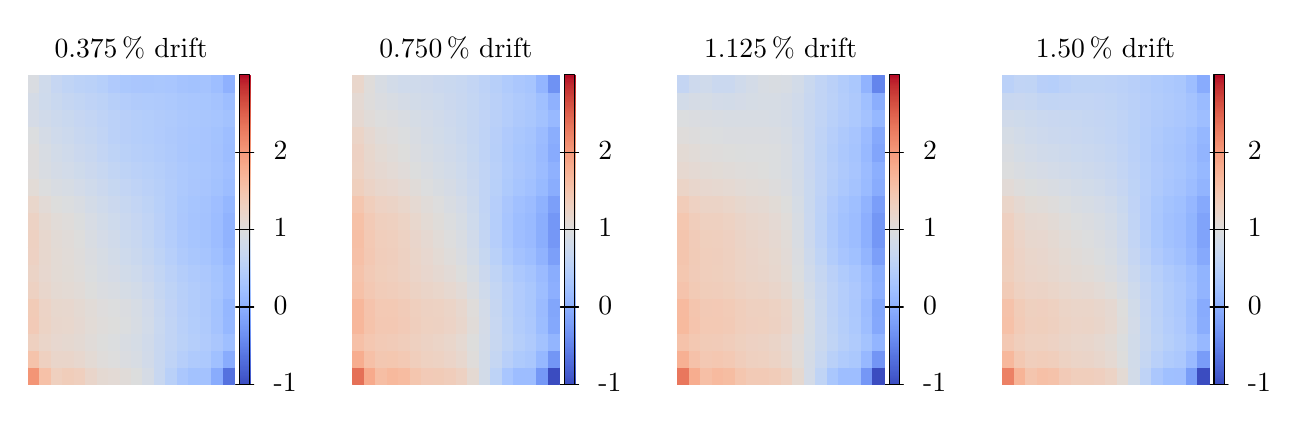
\begin{tikzpicture}[gnuplot]
%% generated with GNUPLOT 5.2p6 (Lua 5.3; terminal rev. Nov 2018, script rev. 107)
%% 03/27/2019 23:35:18
\path (0.000,0.000) rectangle (15.000,4.500);
\gpcolor{color=gp lt color border}
\node[gp node center] at (1.312,4.527) {\SI{0.375}{\percent} drift};
\gpfill{rgb color={0.953,0.583,0.463}} (0.000,0.282)--(0.000,0.501)--(0.146,0.501)--(0.146,0.282)--cycle;
\gpfill{rgb color={0.963,0.757,0.660}} (0.146,0.282)--(0.146,0.501)--(0.292,0.501)--(0.292,0.282)--cycle;
\gpfill{rgb color={0.960,0.765,0.671}} (0.000,0.501)--(0.000,0.719)--(0.146,0.719)--(0.146,0.501)--cycle;
\gpfill{rgb color={0.934,0.817,0.754}} (0.146,0.501)--(0.146,0.719)--(0.292,0.719)--(0.292,0.501)--cycle;
\gpfill{rgb color={0.933,0.817,0.754}} (0.000,0.719)--(0.000,0.938)--(0.146,0.938)--(0.146,0.719)--cycle;
\gpfill{rgb color={0.916,0.835,0.790}} (0.146,0.719)--(0.146,0.938)--(0.292,0.938)--(0.292,0.719)--cycle;
\gpfill{rgb color={0.948,0.794,0.716}} (0.000,0.938)--(0.000,1.157)--(0.146,1.157)--(0.146,0.938)--cycle;
\gpfill{rgb color={0.925,0.826,0.772}} (0.146,0.938)--(0.146,1.157)--(0.292,1.157)--(0.292,0.938)--cycle;
\gpfill{rgb color={0.947,0.796,0.719}} (0.000,1.157)--(0.000,1.376)--(0.146,1.376)--(0.146,1.157)--cycle;
\gpfill{rgb color={0.924,0.828,0.775}} (0.146,1.157)--(0.146,1.376)--(0.292,1.376)--(0.292,1.157)--cycle;
\gpfill{rgb color={0.930,0.821,0.762}} (0.000,1.376)--(0.000,1.594)--(0.146,1.594)--(0.146,1.376)--cycle;
\gpfill{rgb color={0.910,0.840,0.801}} (0.146,1.376)--(0.146,1.594)--(0.292,1.594)--(0.292,1.376)--cycle;
\gpfill{rgb color={0.923,0.829,0.777}} (0.000,1.594)--(0.000,1.813)--(0.146,1.813)--(0.146,1.594)--cycle;
\gpfill{rgb color={0.904,0.845,0.811}} (0.146,1.594)--(0.146,1.813)--(0.292,1.813)--(0.292,1.594)--cycle;
\gpfill{rgb color={0.930,0.821,0.763}} (0.000,1.813)--(0.000,2.032)--(0.146,2.032)--(0.146,1.813)--cycle;
\gpfill{rgb color={0.907,0.843,0.806}} (0.146,1.813)--(0.146,2.032)--(0.292,2.032)--(0.292,1.813)--cycle;
\gpfill{rgb color={0.931,0.820,0.760}} (0.000,2.032)--(0.000,2.250)--(0.146,2.250)--(0.146,2.032)--cycle;
\gpfill{rgb color={0.906,0.843,0.808}} (0.146,2.032)--(0.146,2.250)--(0.292,2.250)--(0.292,2.032)--cycle;
\gpfill{rgb color={0.927,0.824,0.768}} (0.000,2.250)--(0.000,2.468)--(0.146,2.468)--(0.146,2.250)--cycle;
\gpfill{rgb color={0.900,0.847,0.817}} (0.146,2.250)--(0.146,2.468)--(0.292,2.468)--(0.292,2.250)--cycle;
\gpfill{rgb color={0.913,0.838,0.796}} (0.000,2.468)--(0.000,2.687)--(0.146,2.687)--(0.146,2.468)--cycle;
\gpfill{rgb color={0.887,0.856,0.838}} (0.146,2.468)--(0.146,2.687)--(0.292,2.687)--(0.292,2.468)--cycle;
\gpfill{rgb color={0.885,0.857,0.840}} (0.000,2.687)--(0.000,2.906)--(0.146,2.906)--(0.146,2.687)--cycle;
\gpfill{rgb color={0.862,0.865,0.869}} (0.146,2.687)--(0.146,2.906)--(0.292,2.906)--(0.292,2.687)--cycle;
\gpfill{rgb color={0.869,0.864,0.861}} (0.000,2.906)--(0.000,3.124)--(0.146,3.124)--(0.146,2.906)--cycle;
\gpfill{rgb color={0.848,0.863,0.886}} (0.146,2.906)--(0.146,3.124)--(0.292,3.124)--(0.292,2.906)--cycle;
\gpfill{rgb color={0.869,0.864,0.861}} (0.000,3.124)--(0.000,3.343)--(0.146,3.343)--(0.146,3.124)--cycle;
\gpfill{rgb color={0.843,0.862,0.892}} (0.146,3.124)--(0.146,3.343)--(0.292,3.343)--(0.292,3.124)--cycle;
\gpfill{rgb color={0.858,0.865,0.875}} (0.000,3.343)--(0.000,3.562)--(0.146,3.562)--(0.146,3.343)--cycle;
\gpfill{rgb color={0.832,0.860,0.902}} (0.146,3.343)--(0.146,3.562)--(0.292,3.562)--(0.292,3.343)--cycle;
\gpfill{rgb color={0.834,0.860,0.901}} (0.000,3.562)--(0.000,3.781)--(0.146,3.781)--(0.146,3.562)--cycle;
\gpfill{rgb color={0.816,0.855,0.918}} (0.146,3.562)--(0.146,3.781)--(0.292,3.781)--(0.292,3.562)--cycle;
\gpfill{rgb color={0.832,0.860,0.903}} (0.000,3.781)--(0.000,3.999)--(0.146,3.999)--(0.146,3.781)--cycle;
\gpfill{rgb color={0.808,0.853,0.924}} (0.146,3.781)--(0.146,3.999)--(0.292,3.999)--(0.292,3.781)--cycle;
\gpfill{rgb color={0.852,0.864,0.881}} (0.000,3.999)--(0.000,4.218)--(0.146,4.218)--(0.146,3.999)--cycle;
\gpfill{rgb color={0.810,0.854,0.922}} (0.146,3.999)--(0.146,4.218)--(0.292,4.218)--(0.292,3.999)--cycle;
\gpfill{rgb color={0.936,0.814,0.749}} (0.292,0.282)--(0.292,0.501)--(0.438,0.501)--(0.438,0.282)--cycle;
\gpfill{rgb color={0.943,0.803,0.731}} (0.438,0.282)--(0.438,0.501)--(0.583,0.501)--(0.583,0.282)--cycle;
\gpfill{rgb color={0.914,0.837,0.794}} (0.292,0.501)--(0.292,0.719)--(0.438,0.719)--(0.438,0.501)--cycle;
\gpfill{rgb color={0.915,0.836,0.793}} (0.438,0.501)--(0.438,0.719)--(0.583,0.719)--(0.583,0.501)--cycle;
\gpfill{rgb color={0.904,0.845,0.811}} (0.292,0.719)--(0.292,0.938)--(0.438,0.938)--(0.438,0.719)--cycle;
\gpfill{rgb color={0.900,0.847,0.817}} (0.438,0.719)--(0.438,0.938)--(0.583,0.938)--(0.583,0.719)--cycle;
\gpfill{rgb color={0.910,0.840,0.801}} (0.292,0.938)--(0.292,1.157)--(0.438,1.157)--(0.438,0.938)--cycle;
\gpfill{rgb color={0.908,0.842,0.805}} (0.438,0.938)--(0.438,1.157)--(0.583,1.157)--(0.583,0.938)--cycle;
\gpfill{rgb color={0.907,0.842,0.805}} (0.292,1.157)--(0.292,1.376)--(0.438,1.376)--(0.438,1.157)--cycle;
\gpfill{rgb color={0.905,0.844,0.809}} (0.438,1.157)--(0.438,1.376)--(0.583,1.376)--(0.583,1.157)--cycle;
\gpfill{rgb color={0.896,0.850,0.823}} (0.292,1.376)--(0.292,1.594)--(0.438,1.594)--(0.438,1.376)--cycle;
\gpfill{rgb color={0.891,0.853,0.831}} (0.438,1.376)--(0.438,1.594)--(0.583,1.594)--(0.583,1.376)--cycle;
\gpfill{rgb color={0.890,0.854,0.832}} (0.292,1.594)--(0.292,1.813)--(0.438,1.813)--(0.438,1.594)--cycle;
\gpfill{rgb color={0.884,0.857,0.841}} (0.438,1.594)--(0.438,1.813)--(0.583,1.813)--(0.583,1.594)--cycle;
\gpfill{rgb color={0.890,0.854,0.832}} (0.292,1.813)--(0.292,2.032)--(0.438,2.032)--(0.438,1.813)--cycle;
\gpfill{rgb color={0.883,0.857,0.842}} (0.438,1.813)--(0.438,2.032)--(0.583,2.032)--(0.583,1.813)--cycle;
\gpfill{rgb color={0.887,0.855,0.837}} (0.292,2.032)--(0.292,2.250)--(0.438,2.250)--(0.438,2.032)--cycle;
\gpfill{rgb color={0.880,0.859,0.847}} (0.438,2.032)--(0.438,2.250)--(0.583,2.250)--(0.583,2.032)--cycle;
\gpfill{rgb color={0.881,0.859,0.845}} (0.292,2.250)--(0.292,2.468)--(0.438,2.468)--(0.438,2.250)--cycle;
\gpfill{rgb color={0.873,0.862,0.856}} (0.438,2.250)--(0.438,2.468)--(0.583,2.468)--(0.583,2.250)--cycle;
\gpfill{rgb color={0.867,0.865,0.863}} (0.292,2.468)--(0.292,2.687)--(0.438,2.687)--(0.438,2.468)--cycle;
\gpfill{rgb color={0.859,0.865,0.873}} (0.438,2.468)--(0.438,2.687)--(0.583,2.687)--(0.583,2.468)--cycle;
\gpfill{rgb color={0.847,0.863,0.886}} (0.292,2.687)--(0.292,2.906)--(0.438,2.906)--(0.438,2.687)--cycle;
\gpfill{rgb color={0.838,0.861,0.896}} (0.438,2.687)--(0.438,2.906)--(0.583,2.906)--(0.583,2.687)--cycle;
\gpfill{rgb color={0.833,0.860,0.902}} (0.292,2.906)--(0.292,3.124)--(0.438,3.124)--(0.438,2.906)--cycle;
\gpfill{rgb color={0.822,0.857,0.912}} (0.438,2.906)--(0.438,3.124)--(0.583,3.124)--(0.583,2.906)--cycle;
\gpfill{rgb color={0.823,0.858,0.911}} (0.292,3.124)--(0.292,3.343)--(0.438,3.343)--(0.438,3.124)--cycle;
\gpfill{rgb color={0.811,0.854,0.922}} (0.438,3.124)--(0.438,3.343)--(0.583,3.343)--(0.583,3.124)--cycle;
\gpfill{rgb color={0.812,0.854,0.921}} (0.292,3.343)--(0.292,3.562)--(0.438,3.562)--(0.438,3.343)--cycle;
\gpfill{rgb color={0.800,0.850,0.931}} (0.438,3.343)--(0.438,3.562)--(0.583,3.562)--(0.583,3.343)--cycle;
\gpfill{rgb color={0.801,0.850,0.930}} (0.292,3.562)--(0.292,3.781)--(0.438,3.781)--(0.438,3.562)--cycle;
\gpfill{rgb color={0.789,0.846,0.939}} (0.438,3.562)--(0.438,3.781)--(0.583,3.781)--(0.583,3.562)--cycle;
\gpfill{rgb color={0.789,0.846,0.939}} (0.292,3.781)--(0.292,3.999)--(0.438,3.999)--(0.438,3.781)--cycle;
\gpfill{rgb color={0.773,0.840,0.950}} (0.438,3.781)--(0.438,3.999)--(0.583,3.999)--(0.583,3.781)--cycle;
\gpfill{rgb color={0.776,0.841,0.948}} (0.292,3.999)--(0.292,4.218)--(0.438,4.218)--(0.438,3.999)--cycle;
\gpfill{rgb color={0.752,0.830,0.962}} (0.438,3.999)--(0.438,4.218)--(0.583,4.218)--(0.583,3.999)--cycle;
\gpfill{rgb color={0.937,0.812,0.746}} (0.583,0.282)--(0.583,0.501)--(0.729,0.501)--(0.729,0.282)--cycle;
\gpfill{rgb color={0.914,0.837,0.794}} (0.729,0.282)--(0.729,0.501)--(0.875,0.501)--(0.875,0.282)--cycle;
\gpfill{rgb color={0.907,0.843,0.806}} (0.583,0.501)--(0.583,0.719)--(0.729,0.719)--(0.729,0.501)--cycle;
\gpfill{rgb color={0.889,0.854,0.833}} (0.729,0.501)--(0.729,0.719)--(0.875,0.719)--(0.875,0.501)--cycle;
\gpfill{rgb color={0.892,0.852,0.829}} (0.583,0.719)--(0.583,0.938)--(0.729,0.938)--(0.729,0.719)--cycle;
\gpfill{rgb color={0.879,0.860,0.848}} (0.729,0.719)--(0.729,0.938)--(0.875,0.938)--(0.875,0.719)--cycle;
\gpfill{rgb color={0.900,0.848,0.818}} (0.583,0.938)--(0.583,1.157)--(0.729,1.157)--(0.729,0.938)--cycle;
\gpfill{rgb color={0.885,0.857,0.840}} (0.729,0.938)--(0.729,1.157)--(0.875,1.157)--(0.875,0.938)--cycle;
\gpfill{rgb color={0.896,0.850,0.823}} (0.583,1.157)--(0.583,1.376)--(0.729,1.376)--(0.729,1.157)--cycle;
\gpfill{rgb color={0.881,0.859,0.845}} (0.729,1.157)--(0.729,1.376)--(0.875,1.376)--(0.875,1.157)--cycle;
\gpfill{rgb color={0.882,0.858,0.844}} (0.583,1.376)--(0.583,1.594)--(0.729,1.594)--(0.729,1.376)--cycle;
\gpfill{rgb color={0.867,0.865,0.864}} (0.729,1.376)--(0.729,1.594)--(0.875,1.594)--(0.875,1.376)--cycle;
\gpfill{rgb color={0.873,0.862,0.856}} (0.583,1.594)--(0.583,1.813)--(0.729,1.813)--(0.729,1.594)--cycle;
\gpfill{rgb color={0.858,0.865,0.874}} (0.729,1.594)--(0.729,1.813)--(0.875,1.813)--(0.875,1.594)--cycle;
\gpfill{rgb color={0.871,0.863,0.859}} (0.583,1.813)--(0.583,2.032)--(0.729,2.032)--(0.729,1.813)--cycle;
\gpfill{rgb color={0.854,0.864,0.879}} (0.729,1.813)--(0.729,2.032)--(0.875,2.032)--(0.875,1.813)--cycle;
\gpfill{rgb color={0.866,0.865,0.864}} (0.583,2.032)--(0.583,2.250)--(0.729,2.250)--(0.729,2.032)--cycle;
\gpfill{rgb color={0.848,0.863,0.885}} (0.729,2.032)--(0.729,2.250)--(0.875,2.250)--(0.875,2.032)--cycle;
\gpfill{rgb color={0.860,0.865,0.872}} (0.583,2.250)--(0.583,2.468)--(0.729,2.468)--(0.729,2.250)--cycle;
\gpfill{rgb color={0.842,0.862,0.893}} (0.729,2.250)--(0.729,2.468)--(0.875,2.468)--(0.875,2.250)--cycle;
\gpfill{rgb color={0.847,0.863,0.887}} (0.583,2.468)--(0.583,2.687)--(0.729,2.687)--(0.729,2.468)--cycle;
\gpfill{rgb color={0.829,0.859,0.905}} (0.729,2.468)--(0.729,2.687)--(0.875,2.687)--(0.875,2.468)--cycle;
\gpfill{rgb color={0.826,0.858,0.908}} (0.583,2.687)--(0.583,2.906)--(0.729,2.906)--(0.729,2.687)--cycle;
\gpfill{rgb color={0.811,0.854,0.922}} (0.729,2.687)--(0.729,2.906)--(0.875,2.906)--(0.875,2.687)--cycle;
\gpfill{rgb color={0.809,0.853,0.923}} (0.583,2.906)--(0.583,3.124)--(0.729,3.124)--(0.729,2.906)--cycle;
\gpfill{rgb color={0.795,0.848,0.934}} (0.729,2.906)--(0.729,3.124)--(0.875,3.124)--(0.875,2.906)--cycle;
\gpfill{rgb color={0.797,0.849,0.933}} (0.583,3.124)--(0.583,3.343)--(0.729,3.343)--(0.729,3.124)--cycle;
\gpfill{rgb color={0.783,0.844,0.943}} (0.729,3.124)--(0.729,3.343)--(0.875,3.343)--(0.875,3.124)--cycle;
\gpfill{rgb color={0.786,0.845,0.941}} (0.583,3.343)--(0.583,3.562)--(0.729,3.562)--(0.729,3.343)--cycle;
\gpfill{rgb color={0.772,0.839,0.950}} (0.729,3.343)--(0.729,3.562)--(0.875,3.562)--(0.875,3.343)--cycle;
\gpfill{rgb color={0.777,0.841,0.948}} (0.583,3.562)--(0.583,3.781)--(0.729,3.781)--(0.729,3.562)--cycle;
\gpfill{rgb color={0.764,0.836,0.955}} (0.729,3.562)--(0.729,3.781)--(0.875,3.781)--(0.875,3.562)--cycle;
\gpfill{rgb color={0.760,0.834,0.958}} (0.583,3.781)--(0.583,3.999)--(0.729,3.999)--(0.729,3.781)--cycle;
\gpfill{rgb color={0.750,0.829,0.963}} (0.729,3.781)--(0.729,3.999)--(0.875,3.999)--(0.875,3.781)--cycle;
\gpfill{rgb color={0.737,0.822,0.970}} (0.583,3.999)--(0.583,4.218)--(0.729,4.218)--(0.729,3.999)--cycle;
\gpfill{rgb color={0.731,0.819,0.973}} (0.729,3.999)--(0.729,4.218)--(0.875,4.218)--(0.875,3.999)--cycle;
\gpfill{rgb color={0.896,0.850,0.823}} (0.875,0.282)--(0.875,0.501)--(1.021,0.501)--(1.021,0.282)--cycle;
\gpfill{rgb color={0.889,0.854,0.835}} (1.021,0.282)--(1.021,0.501)--(1.167,0.501)--(1.167,0.282)--cycle;
\gpfill{rgb color={0.875,0.861,0.853}} (0.875,0.501)--(0.875,0.719)--(1.021,0.719)--(1.021,0.501)--cycle;
\gpfill{rgb color={0.866,0.865,0.865}} (1.021,0.501)--(1.021,0.719)--(1.167,0.719)--(1.167,0.501)--cycle;
\gpfill{rgb color={0.867,0.865,0.863}} (0.875,0.719)--(0.875,0.938)--(1.021,0.938)--(1.021,0.719)--cycle;
\gpfill{rgb color={0.859,0.865,0.873}} (1.021,0.719)--(1.021,0.938)--(1.167,0.938)--(1.167,0.719)--cycle;
\gpfill{rgb color={0.873,0.862,0.855}} (0.875,0.938)--(0.875,1.157)--(1.021,1.157)--(1.021,0.938)--cycle;
\gpfill{rgb color={0.866,0.865,0.864}} (1.021,0.938)--(1.021,1.157)--(1.167,1.157)--(1.167,0.938)--cycle;
\gpfill{rgb color={0.869,0.864,0.861}} (0.875,1.157)--(0.875,1.376)--(1.021,1.376)--(1.021,1.157)--cycle;
\gpfill{rgb color={0.862,0.865,0.869}} (1.021,1.157)--(1.021,1.376)--(1.167,1.376)--(1.167,1.157)--cycle;
\gpfill{rgb color={0.856,0.864,0.877}} (0.875,1.376)--(0.875,1.594)--(1.021,1.594)--(1.021,1.376)--cycle;
\gpfill{rgb color={0.847,0.863,0.887}} (1.021,1.376)--(1.021,1.594)--(1.167,1.594)--(1.167,1.376)--cycle;
\gpfill{rgb color={0.845,0.863,0.889}} (0.875,1.594)--(0.875,1.813)--(1.021,1.813)--(1.021,1.594)--cycle;
\gpfill{rgb color={0.834,0.860,0.901}} (1.021,1.594)--(1.021,1.813)--(1.167,1.813)--(1.167,1.594)--cycle;
\gpfill{rgb color={0.838,0.861,0.896}} (0.875,1.813)--(0.875,2.032)--(1.021,2.032)--(1.021,1.813)--cycle;
\gpfill{rgb color={0.823,0.858,0.911}} (1.021,1.813)--(1.021,2.032)--(1.167,2.032)--(1.167,1.813)--cycle;
\gpfill{rgb color={0.831,0.860,0.904}} (0.875,2.032)--(0.875,2.250)--(1.021,2.250)--(1.021,2.032)--cycle;
\gpfill{rgb color={0.814,0.855,0.919}} (1.021,2.032)--(1.021,2.250)--(1.167,2.250)--(1.167,2.032)--cycle;
\gpfill{rgb color={0.824,0.858,0.910}} (0.875,2.250)--(0.875,2.468)--(1.021,2.468)--(1.021,2.250)--cycle;
\gpfill{rgb color={0.807,0.853,0.925}} (1.021,2.250)--(1.021,2.468)--(1.167,2.468)--(1.167,2.250)--cycle;
\gpfill{rgb color={0.812,0.854,0.921}} (0.875,2.468)--(0.875,2.687)--(1.021,2.687)--(1.021,2.468)--cycle;
\gpfill{rgb color={0.795,0.848,0.935}} (1.021,2.468)--(1.021,2.687)--(1.167,2.687)--(1.167,2.468)--cycle;
\gpfill{rgb color={0.795,0.848,0.935}} (0.875,2.687)--(0.875,2.906)--(1.021,2.906)--(1.021,2.687)--cycle;
\gpfill{rgb color={0.778,0.842,0.947}} (1.021,2.687)--(1.021,2.906)--(1.167,2.906)--(1.167,2.687)--cycle;
\gpfill{rgb color={0.779,0.842,0.946}} (0.875,2.906)--(0.875,3.124)--(1.021,3.124)--(1.021,2.906)--cycle;
\gpfill{rgb color={0.761,0.834,0.957}} (1.021,2.906)--(1.021,3.124)--(1.167,3.124)--(1.167,2.906)--cycle;
\gpfill{rgb color={0.765,0.836,0.955}} (0.875,3.124)--(0.875,3.343)--(1.021,3.343)--(1.021,3.124)--cycle;
\gpfill{rgb color={0.745,0.826,0.966}} (1.021,3.124)--(1.021,3.343)--(1.167,3.343)--(1.167,3.124)--cycle;
\gpfill{rgb color={0.755,0.831,0.960}} (0.875,3.343)--(0.875,3.562)--(1.021,3.562)--(1.021,3.343)--cycle;
\gpfill{rgb color={0.735,0.821,0.971}} (1.021,3.343)--(1.021,3.562)--(1.167,3.562)--(1.167,3.343)--cycle;
\gpfill{rgb color={0.750,0.829,0.964}} (0.875,3.562)--(0.875,3.781)--(1.021,3.781)--(1.021,3.562)--cycle;
\gpfill{rgb color={0.733,0.820,0.972}} (1.021,3.562)--(1.021,3.781)--(1.167,3.781)--(1.167,3.562)--cycle;
\gpfill{rgb color={0.736,0.822,0.970}} (0.875,3.781)--(0.875,3.999)--(1.021,3.999)--(1.021,3.781)--cycle;
\gpfill{rgb color={0.718,0.811,0.978}} (1.021,3.781)--(1.021,3.999)--(1.167,3.999)--(1.167,3.781)--cycle;
\gpfill{rgb color={0.715,0.810,0.980}} (0.875,3.999)--(0.875,4.218)--(1.021,4.218)--(1.021,3.999)--cycle;
\gpfill{rgb color={0.689,0.794,0.988}} (1.021,3.999)--(1.021,4.218)--(1.167,4.218)--(1.167,3.999)--cycle;
\gpfill{rgb color={0.878,0.860,0.849}} (1.167,0.282)--(1.167,0.501)--(1.312,0.501)--(1.312,0.282)--cycle;
\gpfill{rgb color={0.864,0.865,0.867}} (1.312,0.282)--(1.312,0.501)--(1.457,0.501)--(1.457,0.282)--cycle;
\gpfill{rgb color={0.855,0.864,0.877}} (1.167,0.501)--(1.167,0.719)--(1.312,0.719)--(1.312,0.501)--cycle;
\gpfill{rgb color={0.842,0.862,0.892}} (1.312,0.501)--(1.312,0.719)--(1.457,0.719)--(1.457,0.501)--cycle;
\gpfill{rgb color={0.849,0.863,0.885}} (1.167,0.719)--(1.167,0.938)--(1.312,0.938)--(1.312,0.719)--cycle;
\gpfill{rgb color={0.836,0.861,0.899}} (1.312,0.719)--(1.312,0.938)--(1.457,0.938)--(1.457,0.719)--cycle;
\gpfill{rgb color={0.857,0.865,0.875}} (1.167,0.938)--(1.167,1.157)--(1.312,1.157)--(1.312,0.938)--cycle;
\gpfill{rgb color={0.845,0.863,0.889}} (1.312,0.938)--(1.312,1.157)--(1.457,1.157)--(1.457,0.938)--cycle;
\gpfill{rgb color={0.853,0.864,0.880}} (1.167,1.157)--(1.167,1.376)--(1.312,1.376)--(1.312,1.157)--cycle;
\gpfill{rgb color={0.841,0.862,0.894}} (1.312,1.157)--(1.312,1.376)--(1.457,1.376)--(1.457,1.157)--cycle;
\gpfill{rgb color={0.836,0.861,0.899}} (1.167,1.376)--(1.167,1.594)--(1.312,1.594)--(1.312,1.376)--cycle;
\gpfill{rgb color={0.823,0.857,0.911}} (1.312,1.376)--(1.312,1.594)--(1.457,1.594)--(1.457,1.376)--cycle;
\gpfill{rgb color={0.821,0.857,0.913}} (1.167,1.594)--(1.167,1.813)--(1.312,1.813)--(1.312,1.594)--cycle;
\gpfill{rgb color={0.807,0.853,0.925}} (1.312,1.594)--(1.312,1.813)--(1.457,1.813)--(1.457,1.594)--cycle;
\gpfill{rgb color={0.808,0.853,0.924}} (1.167,1.813)--(1.167,2.032)--(1.312,2.032)--(1.312,1.813)--cycle;
\gpfill{rgb color={0.794,0.848,0.935}} (1.312,1.813)--(1.312,2.032)--(1.457,2.032)--(1.457,1.813)--cycle;
\gpfill{rgb color={0.798,0.850,0.932}} (1.167,2.032)--(1.167,2.250)--(1.312,2.250)--(1.312,2.032)--cycle;
\gpfill{rgb color={0.783,0.844,0.943}} (1.312,2.032)--(1.312,2.250)--(1.457,2.250)--(1.457,2.032)--cycle;
\gpfill{rgb color={0.791,0.847,0.938}} (1.167,2.250)--(1.167,2.468)--(1.312,2.468)--(1.312,2.250)--cycle;
\gpfill{rgb color={0.776,0.841,0.948}} (1.312,2.250)--(1.312,2.468)--(1.457,2.468)--(1.457,2.250)--cycle;
\gpfill{rgb color={0.779,0.842,0.946}} (1.167,2.468)--(1.167,2.687)--(1.312,2.687)--(1.312,2.468)--cycle;
\gpfill{rgb color={0.765,0.836,0.955}} (1.312,2.468)--(1.312,2.687)--(1.457,2.687)--(1.457,2.468)--cycle;
\gpfill{rgb color={0.763,0.835,0.956}} (1.167,2.687)--(1.167,2.906)--(1.312,2.906)--(1.312,2.687)--cycle;
\gpfill{rgb color={0.750,0.829,0.963}} (1.312,2.687)--(1.312,2.906)--(1.457,2.906)--(1.457,2.687)--cycle;
\gpfill{rgb color={0.746,0.827,0.965}} (1.167,2.906)--(1.167,3.124)--(1.312,3.124)--(1.312,2.906)--cycle;
\gpfill{rgb color={0.735,0.821,0.971}} (1.312,2.906)--(1.312,3.124)--(1.457,3.124)--(1.457,2.906)--cycle;
\gpfill{rgb color={0.729,0.818,0.974}} (1.167,3.124)--(1.167,3.343)--(1.312,3.343)--(1.312,3.124)--cycle;
\gpfill{rgb color={0.718,0.812,0.978}} (1.312,3.124)--(1.312,3.343)--(1.457,3.343)--(1.457,3.124)--cycle;
\gpfill{rgb color={0.720,0.813,0.977}} (1.167,3.343)--(1.167,3.562)--(1.312,3.562)--(1.312,3.343)--cycle;
\gpfill{rgb color={0.710,0.807,0.981}} (1.312,3.343)--(1.312,3.562)--(1.457,3.562)--(1.457,3.343)--cycle;
\gpfill{rgb color={0.720,0.813,0.978}} (1.167,3.562)--(1.167,3.781)--(1.312,3.781)--(1.312,3.562)--cycle;
\gpfill{rgb color={0.711,0.807,0.981}} (1.312,3.562)--(1.312,3.781)--(1.457,3.781)--(1.457,3.562)--cycle;
\gpfill{rgb color={0.704,0.803,0.983}} (1.167,3.781)--(1.167,3.999)--(1.312,3.999)--(1.312,3.781)--cycle;
\gpfill{rgb color={0.696,0.798,0.986}} (1.312,3.781)--(1.312,3.999)--(1.457,3.999)--(1.457,3.781)--cycle;
\gpfill{rgb color={0.672,0.783,0.993}} (1.167,3.999)--(1.167,4.218)--(1.312,4.218)--(1.312,3.999)--cycle;
\gpfill{rgb color={0.665,0.778,0.994}} (1.312,3.999)--(1.312,4.218)--(1.457,4.218)--(1.457,3.999)--cycle;
\gpfill{rgb color={0.834,0.860,0.900}} (1.457,0.282)--(1.457,0.501)--(1.603,0.501)--(1.603,0.282)--cycle;
\gpfill{rgb color={0.783,0.844,0.943}} (1.603,0.282)--(1.603,0.501)--(1.749,0.501)--(1.749,0.282)--cycle;
\gpfill{rgb color={0.819,0.856,0.915}} (1.457,0.501)--(1.457,0.719)--(1.603,0.719)--(1.603,0.501)--cycle;
\gpfill{rgb color={0.784,0.844,0.942}} (1.603,0.501)--(1.603,0.719)--(1.749,0.719)--(1.749,0.501)--cycle;
\gpfill{rgb color={0.815,0.855,0.918}} (1.457,0.719)--(1.457,0.938)--(1.603,0.938)--(1.603,0.719)--cycle;
\gpfill{rgb color={0.786,0.845,0.941}} (1.603,0.719)--(1.603,0.938)--(1.749,0.938)--(1.749,0.719)--cycle;
\gpfill{rgb color={0.822,0.857,0.912}} (1.457,0.938)--(1.457,1.157)--(1.603,1.157)--(1.603,0.938)--cycle;
\gpfill{rgb color={0.788,0.846,0.940}} (1.603,0.938)--(1.603,1.157)--(1.749,1.157)--(1.749,0.938)--cycle;
\gpfill{rgb color={0.818,0.856,0.916}} (1.457,1.157)--(1.457,1.376)--(1.603,1.376)--(1.603,1.157)--cycle;
\gpfill{rgb color={0.784,0.844,0.943}} (1.603,1.157)--(1.603,1.376)--(1.749,1.376)--(1.749,1.157)--cycle;
\gpfill{rgb color={0.802,0.851,0.929}} (1.457,1.376)--(1.457,1.594)--(1.603,1.594)--(1.603,1.376)--cycle;
\gpfill{rgb color={0.773,0.840,0.950}} (1.603,1.376)--(1.603,1.594)--(1.749,1.594)--(1.749,1.376)--cycle;
\gpfill{rgb color={0.787,0.845,0.940}} (1.457,1.594)--(1.457,1.813)--(1.603,1.813)--(1.603,1.594)--cycle;
\gpfill{rgb color={0.760,0.834,0.958}} (1.603,1.594)--(1.603,1.813)--(1.749,1.813)--(1.749,1.594)--cycle;
\gpfill{rgb color={0.773,0.839,0.950}} (1.457,1.813)--(1.457,2.032)--(1.603,2.032)--(1.603,1.813)--cycle;
\gpfill{rgb color={0.745,0.826,0.966}} (1.603,1.813)--(1.603,2.032)--(1.749,2.032)--(1.749,1.813)--cycle;
\gpfill{rgb color={0.762,0.835,0.957}} (1.457,2.032)--(1.457,2.250)--(1.603,2.250)--(1.603,2.032)--cycle;
\gpfill{rgb color={0.734,0.820,0.971}} (1.603,2.032)--(1.603,2.250)--(1.749,2.250)--(1.749,2.032)--cycle;
\gpfill{rgb color={0.755,0.831,0.960}} (1.457,2.250)--(1.457,2.468)--(1.603,2.468)--(1.603,2.250)--cycle;
\gpfill{rgb color={0.728,0.817,0.974}} (1.603,2.250)--(1.603,2.468)--(1.749,2.468)--(1.749,2.250)--cycle;
\gpfill{rgb color={0.746,0.827,0.965}} (1.457,2.468)--(1.457,2.687)--(1.603,2.687)--(1.603,2.468)--cycle;
\gpfill{rgb color={0.722,0.814,0.977}} (1.603,2.468)--(1.603,2.687)--(1.749,2.687)--(1.749,2.468)--cycle;
\gpfill{rgb color={0.735,0.821,0.971}} (1.457,2.687)--(1.457,2.906)--(1.603,2.906)--(1.603,2.687)--cycle;
\gpfill{rgb color={0.718,0.811,0.978}} (1.603,2.687)--(1.603,2.906)--(1.749,2.906)--(1.749,2.687)--cycle;
\gpfill{rgb color={0.723,0.814,0.976}} (1.457,2.906)--(1.457,3.124)--(1.603,3.124)--(1.603,2.906)--cycle;
\gpfill{rgb color={0.710,0.807,0.981}} (1.603,2.906)--(1.603,3.124)--(1.749,3.124)--(1.749,2.906)--cycle;
\gpfill{rgb color={0.708,0.806,0.982}} (1.457,3.124)--(1.457,3.343)--(1.603,3.343)--(1.603,3.124)--cycle;
\gpfill{rgb color={0.699,0.800,0.985}} (1.603,3.124)--(1.603,3.343)--(1.749,3.343)--(1.749,3.124)--cycle;
\gpfill{rgb color={0.702,0.802,0.984}} (1.457,3.343)--(1.457,3.562)--(1.603,3.562)--(1.603,3.343)--cycle;
\gpfill{rgb color={0.694,0.797,0.987}} (1.603,3.343)--(1.603,3.562)--(1.749,3.562)--(1.749,3.343)--cycle;
\gpfill{rgb color={0.703,0.802,0.984}} (1.457,3.562)--(1.457,3.781)--(1.603,3.781)--(1.603,3.562)--cycle;
\gpfill{rgb color={0.696,0.798,0.986}} (1.603,3.562)--(1.603,3.781)--(1.749,3.781)--(1.749,3.562)--cycle;
\gpfill{rgb color={0.690,0.795,0.988}} (1.457,3.781)--(1.457,3.999)--(1.603,3.999)--(1.603,3.781)--cycle;
\gpfill{rgb color={0.687,0.792,0.989}} (1.603,3.781)--(1.603,3.999)--(1.749,3.999)--(1.749,3.781)--cycle;
\gpfill{rgb color={0.663,0.777,0.994}} (1.457,3.999)--(1.457,4.218)--(1.603,4.218)--(1.603,3.999)--cycle;
\gpfill{rgb color={0.667,0.779,0.994}} (1.603,3.999)--(1.603,4.218)--(1.749,4.218)--(1.749,3.999)--cycle;
\gpfill{rgb color={0.727,0.817,0.974}} (1.749,0.282)--(1.749,0.501)--(1.895,0.501)--(1.895,0.282)--cycle;
\gpfill{rgb color={0.669,0.780,0.993}} (1.895,0.282)--(1.895,0.501)--(2.041,0.501)--(2.041,0.282)--cycle;
\gpfill{rgb color={0.748,0.828,0.964}} (1.749,0.501)--(1.749,0.719)--(1.895,0.719)--(1.895,0.501)--cycle;
\gpfill{rgb color={0.712,0.808,0.981}} (1.895,0.501)--(1.895,0.719)--(2.041,0.719)--(2.041,0.501)--cycle;
\gpfill{rgb color={0.757,0.832,0.960}} (1.749,0.719)--(1.749,0.938)--(1.895,0.938)--(1.895,0.719)--cycle;
\gpfill{rgb color={0.730,0.818,0.973}} (1.895,0.719)--(1.895,0.938)--(2.041,0.938)--(2.041,0.719)--cycle;
\gpfill{rgb color={0.755,0.831,0.961}} (1.749,0.938)--(1.749,1.157)--(1.895,1.157)--(1.895,0.938)--cycle;
\gpfill{rgb color={0.724,0.815,0.976}} (1.895,0.938)--(1.895,1.157)--(2.041,1.157)--(2.041,0.938)--cycle;
\gpfill{rgb color={0.751,0.829,0.963}} (1.749,1.157)--(1.749,1.376)--(1.895,1.376)--(1.895,1.157)--cycle;
\gpfill{rgb color={0.721,0.813,0.977}} (1.895,1.157)--(1.895,1.376)--(2.041,1.376)--(2.041,1.157)--cycle;
\gpfill{rgb color={0.745,0.826,0.966}} (1.749,1.376)--(1.749,1.594)--(1.895,1.594)--(1.895,1.376)--cycle;
\gpfill{rgb color={0.718,0.812,0.978}} (1.895,1.376)--(1.895,1.594)--(2.041,1.594)--(2.041,1.376)--cycle;
\gpfill{rgb color={0.733,0.820,0.972}} (1.749,1.594)--(1.749,1.813)--(1.895,1.813)--(1.895,1.594)--cycle;
\gpfill{rgb color={0.707,0.805,0.982}} (1.895,1.594)--(1.895,1.813)--(2.041,1.813)--(2.041,1.594)--cycle;
\gpfill{rgb color={0.716,0.810,0.979}} (1.749,1.813)--(1.749,2.032)--(1.895,2.032)--(1.895,1.813)--cycle;
\gpfill{rgb color={0.687,0.793,0.989}} (1.895,1.813)--(1.895,2.032)--(2.041,2.032)--(2.041,1.813)--cycle;
\gpfill{rgb color={0.705,0.804,0.983}} (1.749,2.032)--(1.749,2.250)--(1.895,2.250)--(1.895,2.032)--cycle;
\gpfill{rgb color={0.674,0.784,0.992}} (1.895,2.032)--(1.895,2.250)--(2.041,2.250)--(2.041,2.032)--cycle;
\gpfill{rgb color={0.699,0.800,0.985}} (1.749,2.250)--(1.749,2.468)--(1.895,2.468)--(1.895,2.250)--cycle;
\gpfill{rgb color={0.670,0.781,0.993}} (1.895,2.250)--(1.895,2.468)--(2.041,2.468)--(2.041,2.250)--cycle;
\gpfill{rgb color={0.697,0.799,0.986}} (1.749,2.468)--(1.749,2.687)--(1.895,2.687)--(1.895,2.468)--cycle;
\gpfill{rgb color={0.672,0.783,0.993}} (1.895,2.468)--(1.895,2.687)--(2.041,2.687)--(2.041,2.468)--cycle;
\gpfill{rgb color={0.699,0.800,0.985}} (1.749,2.687)--(1.749,2.906)--(1.895,2.906)--(1.895,2.687)--cycle;
\gpfill{rgb color={0.679,0.788,0.991}} (1.895,2.687)--(1.895,2.906)--(2.041,2.906)--(2.041,2.687)--cycle;
\gpfill{rgb color={0.695,0.798,0.986}} (1.749,2.906)--(1.749,3.124)--(1.895,3.124)--(1.895,2.906)--cycle;
\gpfill{rgb color={0.679,0.787,0.991}} (1.895,2.906)--(1.895,3.124)--(2.041,3.124)--(2.041,2.906)--cycle;
\gpfill{rgb color={0.686,0.792,0.989}} (1.749,3.124)--(1.749,3.343)--(1.895,3.343)--(1.895,3.124)--cycle;
\gpfill{rgb color={0.670,0.782,0.993}} (1.895,3.124)--(1.895,3.343)--(2.041,3.343)--(2.041,3.124)--cycle;
\gpfill{rgb color={0.683,0.790,0.990}} (1.749,3.343)--(1.749,3.562)--(1.895,3.562)--(1.895,3.343)--cycle;
\gpfill{rgb color={0.669,0.781,0.993}} (1.895,3.343)--(1.895,3.562)--(2.041,3.562)--(2.041,3.343)--cycle;
\gpfill{rgb color={0.687,0.792,0.989}} (1.749,3.562)--(1.749,3.781)--(1.895,3.781)--(1.895,3.562)--cycle;
\gpfill{rgb color={0.675,0.785,0.992}} (1.895,3.562)--(1.895,3.781)--(2.041,3.781)--(2.041,3.562)--cycle;
\gpfill{rgb color={0.679,0.788,0.991}} (1.749,3.781)--(1.749,3.999)--(1.895,3.999)--(1.895,3.781)--cycle;
\gpfill{rgb color={0.668,0.780,0.994}} (1.895,3.781)--(1.895,3.999)--(2.041,3.999)--(2.041,3.781)--cycle;
\gpfill{rgb color={0.661,0.775,0.995}} (1.749,3.999)--(1.749,4.218)--(1.895,4.218)--(1.895,3.999)--cycle;
\gpfill{rgb color={0.646,0.765,0.997}} (1.895,3.999)--(1.895,4.218)--(2.041,4.218)--(2.041,3.999)--cycle;
\gpfill{rgb color={0.640,0.760,0.998}} (2.041,0.282)--(2.041,0.501)--(2.186,0.501)--(2.186,0.282)--cycle;
\gpfill{rgb color={0.643,0.762,0.998}} (2.186,0.282)--(2.186,0.501)--(2.332,0.501)--(2.332,0.282)--cycle;
\gpfill{rgb color={0.688,0.793,0.988}} (2.041,0.501)--(2.041,0.719)--(2.186,0.719)--(2.186,0.501)--cycle;
\gpfill{rgb color={0.679,0.787,0.991}} (2.186,0.501)--(2.186,0.719)--(2.332,0.719)--(2.332,0.501)--cycle;
\gpfill{rgb color={0.708,0.806,0.982}} (2.041,0.719)--(2.041,0.938)--(2.186,0.938)--(2.186,0.719)--cycle;
\gpfill{rgb color={0.693,0.797,0.987}} (2.186,0.719)--(2.186,0.938)--(2.332,0.938)--(2.332,0.719)--cycle;
\gpfill{rgb color={0.701,0.802,0.984}} (2.041,0.938)--(2.041,1.157)--(2.186,1.157)--(2.186,0.938)--cycle;
\gpfill{rgb color={0.686,0.792,0.989}} (2.186,0.938)--(2.186,1.157)--(2.332,1.157)--(2.332,0.938)--cycle;
\gpfill{rgb color={0.698,0.799,0.986}} (2.041,1.157)--(2.041,1.376)--(2.186,1.376)--(2.186,1.157)--cycle;
\gpfill{rgb color={0.682,0.789,0.990}} (2.186,1.157)--(2.186,1.376)--(2.332,1.376)--(2.332,1.157)--cycle;
\gpfill{rgb color={0.698,0.799,0.986}} (2.041,1.376)--(2.041,1.594)--(2.186,1.594)--(2.186,1.376)--cycle;
\gpfill{rgb color={0.683,0.790,0.990}} (2.186,1.376)--(2.186,1.594)--(2.332,1.594)--(2.332,1.376)--cycle;
\gpfill{rgb color={0.687,0.793,0.989}} (2.041,1.594)--(2.041,1.813)--(2.186,1.813)--(2.186,1.594)--cycle;
\gpfill{rgb color={0.674,0.784,0.992}} (2.186,1.594)--(2.186,1.813)--(2.332,1.813)--(2.332,1.594)--cycle;
\gpfill{rgb color={0.667,0.779,0.994}} (2.041,1.813)--(2.041,2.032)--(2.186,2.032)--(2.186,1.813)--cycle;
\gpfill{rgb color={0.656,0.771,0.996}} (2.186,1.813)--(2.186,2.032)--(2.332,2.032)--(2.332,1.813)--cycle;
\gpfill{rgb color={0.654,0.771,0.996}} (2.041,2.032)--(2.041,2.250)--(2.186,2.250)--(2.186,2.032)--cycle;
\gpfill{rgb color={0.645,0.764,0.997}} (2.186,2.032)--(2.186,2.250)--(2.332,2.250)--(2.332,2.032)--cycle;
\gpfill{rgb color={0.651,0.768,0.997}} (2.041,2.250)--(2.041,2.468)--(2.186,2.468)--(2.186,2.250)--cycle;
\gpfill{rgb color={0.642,0.762,0.998}} (2.186,2.250)--(2.186,2.468)--(2.332,2.468)--(2.332,2.250)--cycle;
\gpfill{rgb color={0.655,0.771,0.996}} (2.041,2.468)--(2.041,2.687)--(2.186,2.687)--(2.186,2.468)--cycle;
\gpfill{rgb color={0.646,0.765,0.997}} (2.186,2.468)--(2.186,2.687)--(2.332,2.687)--(2.332,2.468)--cycle;
\gpfill{rgb color={0.666,0.778,0.994}} (2.041,2.687)--(2.041,2.906)--(2.186,2.906)--(2.186,2.687)--cycle;
\gpfill{rgb color={0.658,0.773,0.995}} (2.186,2.687)--(2.186,2.906)--(2.332,2.906)--(2.332,2.687)--cycle;
\gpfill{rgb color={0.668,0.780,0.994}} (2.041,2.906)--(2.041,3.124)--(2.186,3.124)--(2.186,2.906)--cycle;
\gpfill{rgb color={0.661,0.776,0.995}} (2.186,2.906)--(2.186,3.124)--(2.332,3.124)--(2.332,2.906)--cycle;
\gpfill{rgb color={0.660,0.775,0.995}} (2.041,3.124)--(2.041,3.343)--(2.186,3.343)--(2.186,3.124)--cycle;
\gpfill{rgb color={0.657,0.773,0.996}} (2.186,3.124)--(2.186,3.343)--(2.332,3.343)--(2.332,3.124)--cycle;
\gpfill{rgb color={0.661,0.775,0.995}} (2.041,3.343)--(2.041,3.562)--(2.186,3.562)--(2.186,3.343)--cycle;
\gpfill{rgb color={0.658,0.773,0.995}} (2.186,3.343)--(2.186,3.562)--(2.332,3.562)--(2.332,3.343)--cycle;
\gpfill{rgb color={0.668,0.780,0.993}} (2.041,3.562)--(2.041,3.781)--(2.186,3.781)--(2.186,3.562)--cycle;
\gpfill{rgb color={0.664,0.778,0.994}} (2.186,3.562)--(2.186,3.781)--(2.332,3.781)--(2.332,3.562)--cycle;
\gpfill{rgb color={0.661,0.776,0.995}} (2.041,3.781)--(2.041,3.999)--(2.186,3.999)--(2.186,3.781)--cycle;
\gpfill{rgb color={0.660,0.775,0.995}} (2.186,3.781)--(2.186,3.999)--(2.332,3.999)--(2.332,3.781)--cycle;
\gpfill{rgb color={0.641,0.761,0.998}} (2.041,3.999)--(2.041,4.218)--(2.186,4.218)--(2.186,3.999)--cycle;
\gpfill{rgb color={0.646,0.764,0.997}} (2.186,3.999)--(2.186,4.218)--(2.332,4.218)--(2.332,3.999)--cycle;
\gpfill{rgb color={0.538,0.676,0.992}} (2.332,0.282)--(2.332,0.501)--(2.478,0.501)--(2.478,0.282)--cycle;
\gpfill{rgb color={0.333,0.446,0.874}} (2.478,0.282)--(2.478,0.501)--(2.624,0.501)--(2.624,0.282)--cycle;
\gpfill{rgb color={0.629,0.752,0.999}} (2.332,0.501)--(2.332,0.719)--(2.478,0.719)--(2.478,0.501)--cycle;
\gpfill{rgb color={0.537,0.674,0.992}} (2.478,0.501)--(2.478,0.719)--(2.624,0.719)--(2.624,0.501)--cycle;
\gpfill{rgb color={0.665,0.778,0.994}} (2.332,0.719)--(2.332,0.938)--(2.478,0.938)--(2.478,0.719)--cycle;
\gpfill{rgb color={0.624,0.748,0.999}} (2.478,0.719)--(2.478,0.938)--(2.624,0.938)--(2.624,0.719)--cycle;
\gpfill{rgb color={0.649,0.766,0.997}} (2.332,0.938)--(2.332,1.157)--(2.478,1.157)--(2.478,0.938)--cycle;
\gpfill{rgb color={0.589,0.720,1.000}} (2.478,0.938)--(2.478,1.157)--(2.624,1.157)--(2.624,0.938)--cycle;
\gpfill{rgb color={0.645,0.764,0.997}} (2.332,1.157)--(2.332,1.376)--(2.478,1.376)--(2.478,1.157)--cycle;
\gpfill{rgb color={0.586,0.717,0.999}} (2.478,1.157)--(2.478,1.376)--(2.624,1.376)--(2.624,1.157)--cycle;
\gpfill{rgb color={0.655,0.771,0.996}} (2.332,1.376)--(2.332,1.594)--(2.478,1.594)--(2.478,1.376)--cycle;
\gpfill{rgb color={0.614,0.740,1.000}} (2.478,1.376)--(2.478,1.594)--(2.624,1.594)--(2.624,1.376)--cycle;
\gpfill{rgb color={0.649,0.767,0.997}} (2.332,1.594)--(2.332,1.813)--(2.478,1.813)--(2.478,1.594)--cycle;
\gpfill{rgb color={0.613,0.740,1.000}} (2.478,1.594)--(2.478,1.813)--(2.624,1.813)--(2.624,1.594)--cycle;
\gpfill{rgb color={0.628,0.751,0.999}} (2.332,1.813)--(2.332,2.032)--(2.478,2.032)--(2.478,1.813)--cycle;
\gpfill{rgb color={0.584,0.716,0.999}} (2.478,1.813)--(2.478,2.032)--(2.624,2.032)--(2.624,1.813)--cycle;
\gpfill{rgb color={0.617,0.742,1.000}} (2.332,2.032)--(2.332,2.250)--(2.478,2.250)--(2.478,2.032)--cycle;
\gpfill{rgb color={0.569,0.703,0.998}} (2.478,2.032)--(2.478,2.250)--(2.624,2.250)--(2.624,2.032)--cycle;
\gpfill{rgb color={0.615,0.741,1.000}} (2.332,2.250)--(2.332,2.468)--(2.478,2.468)--(2.478,2.250)--cycle;
\gpfill{rgb color={0.568,0.702,0.998}} (2.478,2.250)--(2.478,2.468)--(2.624,2.468)--(2.624,2.250)--cycle;
\gpfill{rgb color={0.623,0.747,1.000}} (2.332,2.468)--(2.332,2.687)--(2.478,2.687)--(2.478,2.468)--cycle;
\gpfill{rgb color={0.584,0.716,0.999}} (2.478,2.468)--(2.478,2.687)--(2.624,2.687)--(2.624,2.468)--cycle;
\gpfill{rgb color={0.641,0.761,0.998}} (2.332,2.687)--(2.332,2.906)--(2.478,2.906)--(2.478,2.687)--cycle;
\gpfill{rgb color={0.615,0.741,1.000}} (2.478,2.687)--(2.478,2.906)--(2.624,2.906)--(2.624,2.687)--cycle;
\gpfill{rgb color={0.648,0.766,0.997}} (2.332,2.906)--(2.332,3.124)--(2.478,3.124)--(2.478,2.906)--cycle;
\gpfill{rgb color={0.626,0.749,0.999}} (2.478,2.906)--(2.478,3.124)--(2.624,3.124)--(2.624,2.906)--cycle;
\gpfill{rgb color={0.642,0.762,0.998}} (2.332,3.124)--(2.332,3.343)--(2.478,3.343)--(2.478,3.124)--cycle;
\gpfill{rgb color={0.616,0.742,1.000}} (2.478,3.124)--(2.478,3.343)--(2.624,3.343)--(2.624,3.124)--cycle;
\gpfill{rgb color={0.645,0.764,0.997}} (2.332,3.343)--(2.332,3.562)--(2.478,3.562)--(2.478,3.343)--cycle;
\gpfill{rgb color={0.620,0.745,1.000}} (2.478,3.343)--(2.478,3.562)--(2.624,3.562)--(2.624,3.343)--cycle;
\gpfill{rgb color={0.655,0.771,0.996}} (2.332,3.562)--(2.332,3.781)--(2.478,3.781)--(2.478,3.562)--cycle;
\gpfill{rgb color={0.639,0.759,0.998}} (2.478,3.562)--(2.478,3.781)--(2.624,3.781)--(2.624,3.562)--cycle;
\gpfill{rgb color={0.646,0.765,0.997}} (2.332,3.781)--(2.332,3.999)--(2.478,3.999)--(2.478,3.781)--cycle;
\gpfill{rgb color={0.619,0.744,1.000}} (2.478,3.781)--(2.478,3.999)--(2.624,3.999)--(2.624,3.781)--cycle;
\gpfill{rgb color={0.619,0.744,1.000}} (2.332,3.999)--(2.332,4.218)--(2.478,4.218)--(2.478,3.999)--cycle;
\gpfill{rgb color={0.559,0.695,0.996}} (2.478,3.999)--(2.478,4.218)--(2.624,4.218)--(2.624,3.999)--cycle;
\gpfill{rgb color={0.230,0.299,0.754}} (2.690,0.282)--(2.821,0.282)--(2.821,0.298)--(2.690,0.298)--cycle;
\gpfill{rgb color={0.234,0.306,0.760}} (2.690,0.297)--(2.821,0.297)--(2.821,0.313)--(2.690,0.313)--cycle;
\gpfill{rgb color={0.239,0.312,0.766}} (2.690,0.312)--(2.821,0.312)--(2.821,0.329)--(2.690,0.329)--cycle;
\gpfill{rgb color={0.244,0.320,0.772}} (2.690,0.328)--(2.821,0.328)--(2.821,0.344)--(2.690,0.344)--cycle;
\gpfill{rgb color={0.248,0.326,0.778}} (2.690,0.343)--(2.821,0.343)--(2.821,0.359)--(2.690,0.359)--cycle;
\gpfill{rgb color={0.252,0.333,0.784}} (2.690,0.358)--(2.821,0.358)--(2.821,0.375)--(2.690,0.375)--cycle;
\gpfill{rgb color={0.257,0.340,0.790}} (2.690,0.374)--(2.821,0.374)--(2.821,0.390)--(2.690,0.390)--cycle;
\gpfill{rgb color={0.262,0.347,0.796}} (2.690,0.389)--(2.821,0.389)--(2.821,0.406)--(2.690,0.406)--cycle;
\gpfill{rgb color={0.267,0.354,0.802}} (2.690,0.405)--(2.821,0.405)--(2.821,0.421)--(2.690,0.421)--cycle;
\gpfill{rgb color={0.271,0.360,0.807}} (2.690,0.420)--(2.821,0.420)--(2.821,0.436)--(2.690,0.436)--cycle;
\gpfill{rgb color={0.276,0.367,0.813}} (2.690,0.435)--(2.821,0.435)--(2.821,0.452)--(2.690,0.452)--cycle;
\gpfill{rgb color={0.280,0.374,0.819}} (2.690,0.451)--(2.821,0.451)--(2.821,0.467)--(2.690,0.467)--cycle;
\gpfill{rgb color={0.285,0.380,0.824}} (2.690,0.466)--(2.821,0.466)--(2.821,0.482)--(2.690,0.482)--cycle;
\gpfill{rgb color={0.290,0.387,0.829}} (2.690,0.481)--(2.821,0.481)--(2.821,0.498)--(2.690,0.498)--cycle;
\gpfill{rgb color={0.295,0.394,0.835}} (2.690,0.497)--(2.821,0.497)--(2.821,0.513)--(2.690,0.513)--cycle;
\gpfill{rgb color={0.299,0.400,0.840}} (2.690,0.512)--(2.821,0.512)--(2.821,0.529)--(2.690,0.529)--cycle;
\gpfill{rgb color={0.304,0.407,0.845}} (2.690,0.528)--(2.821,0.528)--(2.821,0.544)--(2.690,0.544)--cycle;
\gpfill{rgb color={0.309,0.413,0.850}} (2.690,0.543)--(2.821,0.543)--(2.821,0.559)--(2.690,0.559)--cycle;
\gpfill{rgb color={0.314,0.420,0.855}} (2.690,0.558)--(2.821,0.558)--(2.821,0.575)--(2.690,0.575)--cycle;
\gpfill{rgb color={0.319,0.427,0.860}} (2.690,0.574)--(2.821,0.574)--(2.821,0.590)--(2.690,0.590)--cycle;
\gpfill{rgb color={0.323,0.433,0.865}} (2.690,0.589)--(2.821,0.589)--(2.821,0.605)--(2.690,0.605)--cycle;
\gpfill{rgb color={0.328,0.439,0.870}} (2.690,0.604)--(2.821,0.604)--(2.821,0.621)--(2.690,0.621)--cycle;
\gpfill{rgb color={0.333,0.446,0.875}} (2.690,0.620)--(2.821,0.620)--(2.821,0.636)--(2.690,0.636)--cycle;
\gpfill{rgb color={0.338,0.452,0.879}} (2.690,0.635)--(2.821,0.635)--(2.821,0.652)--(2.690,0.652)--cycle;
\gpfill{rgb color={0.343,0.459,0.884}} (2.690,0.651)--(2.821,0.651)--(2.821,0.667)--(2.690,0.667)--cycle;
\gpfill{rgb color={0.348,0.465,0.888}} (2.690,0.666)--(2.821,0.666)--(2.821,0.682)--(2.690,0.682)--cycle;
\gpfill{rgb color={0.353,0.472,0.893}} (2.690,0.681)--(2.821,0.681)--(2.821,0.698)--(2.690,0.698)--cycle;
\gpfill{rgb color={0.358,0.478,0.897}} (2.690,0.697)--(2.821,0.697)--(2.821,0.713)--(2.690,0.713)--cycle;
\gpfill{rgb color={0.363,0.485,0.901}} (2.690,0.712)--(2.821,0.712)--(2.821,0.728)--(2.690,0.728)--cycle;
\gpfill{rgb color={0.368,0.491,0.905}} (2.690,0.727)--(2.821,0.727)--(2.821,0.744)--(2.690,0.744)--cycle;
\gpfill{rgb color={0.373,0.497,0.910}} (2.690,0.743)--(2.821,0.743)--(2.821,0.759)--(2.690,0.759)--cycle;
\gpfill{rgb color={0.378,0.503,0.914}} (2.690,0.758)--(2.821,0.758)--(2.821,0.775)--(2.690,0.775)--cycle;
\gpfill{rgb color={0.383,0.510,0.918}} (2.690,0.774)--(2.821,0.774)--(2.821,0.790)--(2.690,0.790)--cycle;
\gpfill{rgb color={0.388,0.516,0.921}} (2.690,0.789)--(2.821,0.789)--(2.821,0.805)--(2.690,0.805)--cycle;
\gpfill{rgb color={0.393,0.522,0.925}} (2.690,0.804)--(2.821,0.804)--(2.821,0.821)--(2.690,0.821)--cycle;
\gpfill{rgb color={0.399,0.528,0.929}} (2.690,0.820)--(2.821,0.820)--(2.821,0.836)--(2.690,0.836)--cycle;
\gpfill{rgb color={0.404,0.534,0.932}} (2.690,0.835)--(2.821,0.835)--(2.821,0.851)--(2.690,0.851)--cycle;
\gpfill{rgb color={0.409,0.540,0.936}} (2.690,0.850)--(2.821,0.850)--(2.821,0.867)--(2.690,0.867)--cycle;
\gpfill{rgb color={0.414,0.546,0.939}} (2.690,0.866)--(2.821,0.866)--(2.821,0.882)--(2.690,0.882)--cycle;
\gpfill{rgb color={0.419,0.552,0.942}} (2.690,0.881)--(2.821,0.881)--(2.821,0.898)--(2.690,0.898)--cycle;
\gpfill{rgb color={0.425,0.559,0.946}} (2.690,0.897)--(2.821,0.897)--(2.821,0.913)--(2.690,0.913)--cycle;
\gpfill{rgb color={0.430,0.564,0.949}} (2.690,0.912)--(2.821,0.912)--(2.821,0.928)--(2.690,0.928)--cycle;
\gpfill{rgb color={0.435,0.570,0.952}} (2.690,0.927)--(2.821,0.927)--(2.821,0.944)--(2.690,0.944)--cycle;
\gpfill{rgb color={0.440,0.576,0.955}} (2.690,0.943)--(2.821,0.943)--(2.821,0.959)--(2.690,0.959)--cycle;
\gpfill{rgb color={0.446,0.582,0.958}} (2.690,0.958)--(2.821,0.958)--(2.821,0.974)--(2.690,0.974)--cycle;
\gpfill{rgb color={0.451,0.587,0.960}} (2.690,0.973)--(2.821,0.973)--(2.821,0.990)--(2.690,0.990)--cycle;
\gpfill{rgb color={0.456,0.593,0.963}} (2.690,0.989)--(2.821,0.989)--(2.821,1.005)--(2.690,1.005)--cycle;
\gpfill{rgb color={0.461,0.599,0.966}} (2.690,1.004)--(2.821,1.004)--(2.821,1.021)--(2.690,1.021)--cycle;
\gpfill{rgb color={0.467,0.605,0.968}} (2.690,1.020)--(2.821,1.020)--(2.821,1.036)--(2.690,1.036)--cycle;
\gpfill{rgb color={0.472,0.610,0.971}} (2.690,1.035)--(2.821,1.035)--(2.821,1.051)--(2.690,1.051)--cycle;
\gpfill{rgb color={0.477,0.616,0.973}} (2.690,1.050)--(2.821,1.050)--(2.821,1.067)--(2.690,1.067)--cycle;
\gpfill{rgb color={0.483,0.622,0.975}} (2.690,1.066)--(2.821,1.066)--(2.821,1.082)--(2.690,1.082)--cycle;
\gpfill{rgb color={0.488,0.627,0.977}} (2.690,1.081)--(2.821,1.081)--(2.821,1.097)--(2.690,1.097)--cycle;
\gpfill{rgb color={0.494,0.632,0.979}} (2.690,1.096)--(2.821,1.096)--(2.821,1.113)--(2.690,1.113)--cycle;
\gpfill{rgb color={0.499,0.638,0.981}} (2.690,1.112)--(2.821,1.112)--(2.821,1.128)--(2.690,1.128)--cycle;
\gpfill{rgb color={0.504,0.643,0.983}} (2.690,1.127)--(2.821,1.127)--(2.821,1.144)--(2.690,1.144)--cycle;
\gpfill{rgb color={0.510,0.649,0.985}} (2.690,1.143)--(2.821,1.143)--(2.821,1.159)--(2.690,1.159)--cycle;
\gpfill{rgb color={0.515,0.654,0.987}} (2.690,1.158)--(2.821,1.158)--(2.821,1.174)--(2.690,1.174)--cycle;
\gpfill{rgb color={0.521,0.659,0.988}} (2.690,1.173)--(2.821,1.173)--(2.821,1.190)--(2.690,1.190)--cycle;
\gpfill{rgb color={0.526,0.664,0.990}} (2.690,1.189)--(2.821,1.189)--(2.821,1.205)--(2.690,1.205)--cycle;
\gpfill{rgb color={0.531,0.669,0.991}} (2.690,1.204)--(2.821,1.204)--(2.821,1.220)--(2.690,1.220)--cycle;
\gpfill{rgb color={0.537,0.674,0.992}} (2.690,1.219)--(2.821,1.219)--(2.821,1.236)--(2.690,1.236)--cycle;
\gpfill{rgb color={0.542,0.679,0.993}} (2.690,1.235)--(2.821,1.235)--(2.821,1.251)--(2.690,1.251)--cycle;
\gpfill{rgb color={0.548,0.684,0.994}} (2.690,1.250)--(2.821,1.250)--(2.821,1.267)--(2.690,1.267)--cycle;
\gpfill{rgb color={0.553,0.689,0.995}} (2.690,1.266)--(2.821,1.266)--(2.821,1.282)--(2.690,1.282)--cycle;
\gpfill{rgb color={0.559,0.694,0.996}} (2.690,1.281)--(2.821,1.281)--(2.821,1.297)--(2.690,1.297)--cycle;
\gpfill{rgb color={0.564,0.699,0.997}} (2.690,1.296)--(2.821,1.296)--(2.821,1.313)--(2.690,1.313)--cycle;
\gpfill{rgb color={0.570,0.704,0.998}} (2.690,1.312)--(2.821,1.312)--(2.821,1.328)--(2.690,1.328)--cycle;
\gpfill{rgb color={0.575,0.708,0.998}} (2.690,1.327)--(2.821,1.327)--(2.821,1.343)--(2.690,1.343)--cycle;
\gpfill{rgb color={0.580,0.713,0.999}} (2.690,1.342)--(2.821,1.342)--(2.821,1.359)--(2.690,1.359)--cycle;
\gpfill{rgb color={0.586,0.717,0.999}} (2.690,1.358)--(2.821,1.358)--(2.821,1.374)--(2.690,1.374)--cycle;
\gpfill{rgb color={0.591,0.722,1.000}} (2.690,1.373)--(2.821,1.373)--(2.821,1.390)--(2.690,1.390)--cycle;
\gpfill{rgb color={0.597,0.726,1.000}} (2.690,1.389)--(2.821,1.389)--(2.821,1.405)--(2.690,1.405)--cycle;
\gpfill{rgb color={0.602,0.731,1.000}} (2.690,1.404)--(2.821,1.404)--(2.821,1.420)--(2.690,1.420)--cycle;
\gpfill{rgb color={0.607,0.735,1.000}} (2.690,1.419)--(2.821,1.419)--(2.821,1.436)--(2.690,1.436)--cycle;
\gpfill{rgb color={0.613,0.739,1.000}} (2.690,1.435)--(2.821,1.435)--(2.821,1.451)--(2.690,1.451)--cycle;
\gpfill{rgb color={0.618,0.744,1.000}} (2.690,1.450)--(2.821,1.450)--(2.821,1.466)--(2.690,1.466)--cycle;
\gpfill{rgb color={0.623,0.748,0.999}} (2.690,1.465)--(2.821,1.465)--(2.821,1.482)--(2.690,1.482)--cycle;
\gpfill{rgb color={0.629,0.752,0.999}} (2.690,1.481)--(2.821,1.481)--(2.821,1.497)--(2.690,1.497)--cycle;
\gpfill{rgb color={0.634,0.756,0.999}} (2.690,1.496)--(2.821,1.496)--(2.821,1.513)--(2.690,1.513)--cycle;
\gpfill{rgb color={0.640,0.760,0.998}} (2.690,1.512)--(2.821,1.512)--(2.821,1.528)--(2.690,1.528)--cycle;
\gpfill{rgb color={0.645,0.764,0.997}} (2.690,1.527)--(2.821,1.527)--(2.821,1.543)--(2.690,1.543)--cycle;
\gpfill{rgb color={0.650,0.767,0.997}} (2.690,1.542)--(2.821,1.542)--(2.821,1.559)--(2.690,1.559)--cycle;
\gpfill{rgb color={0.655,0.771,0.996}} (2.690,1.558)--(2.821,1.558)--(2.821,1.574)--(2.690,1.574)--cycle;
\gpfill{rgb color={0.661,0.775,0.995}} (2.690,1.573)--(2.821,1.573)--(2.821,1.589)--(2.690,1.589)--cycle;
\gpfill{rgb color={0.666,0.778,0.994}} (2.690,1.588)--(2.821,1.588)--(2.821,1.605)--(2.690,1.605)--cycle;
\gpfill{rgb color={0.671,0.782,0.993}} (2.690,1.604)--(2.821,1.604)--(2.821,1.620)--(2.690,1.620)--cycle;
\gpfill{rgb color={0.676,0.786,0.992}} (2.690,1.619)--(2.821,1.619)--(2.821,1.636)--(2.690,1.636)--cycle;
\gpfill{rgb color={0.682,0.789,0.990}} (2.690,1.635)--(2.821,1.635)--(2.821,1.651)--(2.690,1.651)--cycle;
\gpfill{rgb color={0.687,0.792,0.989}} (2.690,1.650)--(2.821,1.650)--(2.821,1.666)--(2.690,1.666)--cycle;
\gpfill{rgb color={0.692,0.796,0.987}} (2.690,1.665)--(2.821,1.665)--(2.821,1.682)--(2.690,1.682)--cycle;
\gpfill{rgb color={0.697,0.799,0.986}} (2.690,1.681)--(2.821,1.681)--(2.821,1.697)--(2.690,1.697)--cycle;
\gpfill{rgb color={0.702,0.802,0.984}} (2.690,1.696)--(2.821,1.696)--(2.821,1.712)--(2.690,1.712)--cycle;
\gpfill{rgb color={0.707,0.805,0.982}} (2.690,1.711)--(2.821,1.711)--(2.821,1.728)--(2.690,1.728)--cycle;
\gpfill{rgb color={0.712,0.808,0.980}} (2.690,1.727)--(2.821,1.727)--(2.821,1.743)--(2.690,1.743)--cycle;
\gpfill{rgb color={0.717,0.811,0.979}} (2.690,1.742)--(2.821,1.742)--(2.821,1.759)--(2.690,1.759)--cycle;
\gpfill{rgb color={0.723,0.814,0.976}} (2.690,1.758)--(2.821,1.758)--(2.821,1.774)--(2.690,1.774)--cycle;
\gpfill{rgb color={0.727,0.817,0.974}} (2.690,1.773)--(2.821,1.773)--(2.821,1.789)--(2.690,1.789)--cycle;
\gpfill{rgb color={0.732,0.820,0.972}} (2.690,1.788)--(2.821,1.788)--(2.821,1.805)--(2.690,1.805)--cycle;
\gpfill{rgb color={0.737,0.822,0.970}} (2.690,1.804)--(2.821,1.804)--(2.821,1.820)--(2.690,1.820)--cycle;
\gpfill{rgb color={0.742,0.825,0.967}} (2.690,1.819)--(2.821,1.819)--(2.821,1.835)--(2.690,1.835)--cycle;
\gpfill{rgb color={0.747,0.827,0.965}} (2.690,1.834)--(2.821,1.834)--(2.821,1.851)--(2.690,1.851)--cycle;
\gpfill{rgb color={0.752,0.830,0.962}} (2.690,1.850)--(2.821,1.850)--(2.821,1.866)--(2.690,1.866)--cycle;
\gpfill{rgb color={0.757,0.832,0.960}} (2.690,1.865)--(2.821,1.865)--(2.821,1.882)--(2.690,1.882)--cycle;
\gpfill{rgb color={0.762,0.834,0.957}} (2.690,1.881)--(2.821,1.881)--(2.821,1.897)--(2.690,1.897)--cycle;
\gpfill{rgb color={0.766,0.837,0.954}} (2.690,1.896)--(2.821,1.896)--(2.821,1.912)--(2.690,1.912)--cycle;
\gpfill{rgb color={0.771,0.839,0.951}} (2.690,1.911)--(2.821,1.911)--(2.821,1.928)--(2.690,1.928)--cycle;
\gpfill{rgb color={0.776,0.841,0.948}} (2.690,1.927)--(2.821,1.927)--(2.821,1.943)--(2.690,1.943)--cycle;
\gpfill{rgb color={0.781,0.843,0.945}} (2.690,1.942)--(2.821,1.942)--(2.821,1.958)--(2.690,1.958)--cycle;
\gpfill{rgb color={0.785,0.845,0.942}} (2.690,1.957)--(2.821,1.957)--(2.821,1.974)--(2.690,1.974)--cycle;
\gpfill{rgb color={0.790,0.846,0.938}} (2.690,1.973)--(2.821,1.973)--(2.821,1.989)--(2.690,1.989)--cycle;
\gpfill{rgb color={0.794,0.848,0.935}} (2.690,1.988)--(2.821,1.988)--(2.821,2.005)--(2.690,2.005)--cycle;
\gpfill{rgb color={0.799,0.850,0.931}} (2.690,2.004)--(2.821,2.004)--(2.821,2.020)--(2.690,2.020)--cycle;
\gpfill{rgb color={0.803,0.851,0.928}} (2.690,2.019)--(2.821,2.019)--(2.821,2.035)--(2.690,2.035)--cycle;
\gpfill{rgb color={0.808,0.853,0.924}} (2.690,2.034)--(2.821,2.034)--(2.821,2.051)--(2.690,2.051)--cycle;
\gpfill{rgb color={0.812,0.854,0.921}} (2.690,2.050)--(2.821,2.050)--(2.821,2.066)--(2.690,2.066)--cycle;
\gpfill{rgb color={0.817,0.856,0.917}} (2.690,2.065)--(2.821,2.065)--(2.821,2.081)--(2.690,2.081)--cycle;
\gpfill{rgb color={0.821,0.857,0.913}} (2.690,2.080)--(2.821,2.080)--(2.821,2.097)--(2.690,2.097)--cycle;
\gpfill{rgb color={0.825,0.858,0.909}} (2.690,2.096)--(2.821,2.096)--(2.821,2.112)--(2.690,2.112)--cycle;
\gpfill{rgb color={0.829,0.859,0.905}} (2.690,2.111)--(2.821,2.111)--(2.821,2.128)--(2.690,2.128)--cycle;
\gpfill{rgb color={0.834,0.860,0.901}} (2.690,2.127)--(2.821,2.127)--(2.821,2.143)--(2.690,2.143)--cycle;
\gpfill{rgb color={0.838,0.861,0.897}} (2.690,2.142)--(2.821,2.142)--(2.821,2.158)--(2.690,2.158)--cycle;
\gpfill{rgb color={0.842,0.862,0.893}} (2.690,2.157)--(2.821,2.157)--(2.821,2.174)--(2.690,2.174)--cycle;
\gpfill{rgb color={0.846,0.863,0.888}} (2.690,2.173)--(2.821,2.173)--(2.821,2.189)--(2.690,2.189)--cycle;
\gpfill{rgb color={0.850,0.863,0.884}} (2.690,2.188)--(2.821,2.188)--(2.821,2.204)--(2.690,2.204)--cycle;
\gpfill{rgb color={0.854,0.864,0.879}} (2.690,2.203)--(2.821,2.203)--(2.821,2.220)--(2.690,2.220)--cycle;
\gpfill{rgb color={0.858,0.865,0.875}} (2.690,2.219)--(2.821,2.219)--(2.821,2.235)--(2.690,2.235)--cycle;
\gpfill{rgb color={0.862,0.865,0.870}} (2.690,2.234)--(2.821,2.234)--(2.821,2.251)--(2.690,2.251)--cycle;
\gpfill{rgb color={0.866,0.865,0.865}} (2.690,2.250)--(2.821,2.250)--(2.821,2.266)--(2.690,2.266)--cycle;
\gpfill{rgb color={0.870,0.864,0.860}} (2.690,2.265)--(2.821,2.265)--(2.821,2.281)--(2.690,2.281)--cycle;
\gpfill{rgb color={0.874,0.862,0.854}} (2.690,2.280)--(2.821,2.280)--(2.821,2.297)--(2.690,2.297)--cycle;
\gpfill{rgb color={0.878,0.860,0.849}} (2.690,2.296)--(2.821,2.296)--(2.821,2.312)--(2.690,2.312)--cycle;
\gpfill{rgb color={0.882,0.858,0.843}} (2.690,2.311)--(2.821,2.311)--(2.821,2.327)--(2.690,2.327)--cycle;
\gpfill{rgb color={0.886,0.856,0.838}} (2.690,2.326)--(2.821,2.326)--(2.821,2.343)--(2.690,2.343)--cycle;
\gpfill{rgb color={0.890,0.853,0.832}} (2.690,2.342)--(2.821,2.342)--(2.821,2.358)--(2.690,2.358)--cycle;
\gpfill{rgb color={0.894,0.851,0.826}} (2.690,2.357)--(2.821,2.357)--(2.821,2.374)--(2.690,2.374)--cycle;
\gpfill{rgb color={0.898,0.849,0.821}} (2.690,2.373)--(2.821,2.373)--(2.821,2.389)--(2.690,2.389)--cycle;
\gpfill{rgb color={0.902,0.846,0.815}} (2.690,2.388)--(2.821,2.388)--(2.821,2.404)--(2.690,2.404)--cycle;
\gpfill{rgb color={0.905,0.844,0.809}} (2.690,2.403)--(2.821,2.403)--(2.821,2.420)--(2.690,2.420)--cycle;
\gpfill{rgb color={0.909,0.841,0.803}} (2.690,2.419)--(2.821,2.419)--(2.821,2.435)--(2.690,2.435)--cycle;
\gpfill{rgb color={0.912,0.839,0.798}} (2.690,2.434)--(2.821,2.434)--(2.821,2.450)--(2.690,2.450)--cycle;
\gpfill{rgb color={0.915,0.836,0.792}} (2.690,2.449)--(2.821,2.449)--(2.821,2.466)--(2.690,2.466)--cycle;
\gpfill{rgb color={0.918,0.833,0.786}} (2.690,2.465)--(2.821,2.465)--(2.821,2.481)--(2.690,2.481)--cycle;
\gpfill{rgb color={0.921,0.830,0.780}} (2.690,2.480)--(2.821,2.480)--(2.821,2.497)--(2.690,2.497)--cycle;
\gpfill{rgb color={0.924,0.827,0.774}} (2.690,2.496)--(2.821,2.496)--(2.821,2.512)--(2.690,2.512)--cycle;
\gpfill{rgb color={0.927,0.824,0.768}} (2.690,2.511)--(2.821,2.511)--(2.821,2.527)--(2.690,2.527)--cycle;
\gpfill{rgb color={0.930,0.821,0.763}} (2.690,2.526)--(2.821,2.526)--(2.821,2.543)--(2.690,2.543)--cycle;
\gpfill{rgb color={0.933,0.818,0.756}} (2.690,2.542)--(2.821,2.542)--(2.821,2.558)--(2.690,2.558)--cycle;
\gpfill{rgb color={0.935,0.815,0.751}} (2.690,2.557)--(2.821,2.557)--(2.821,2.573)--(2.690,2.573)--cycle;
\gpfill{rgb color={0.938,0.811,0.745}} (2.690,2.572)--(2.821,2.572)--(2.821,2.589)--(2.690,2.589)--cycle;
\gpfill{rgb color={0.940,0.808,0.738}} (2.690,2.588)--(2.821,2.588)--(2.821,2.604)--(2.690,2.604)--cycle;
\gpfill{rgb color={0.942,0.804,0.733}} (2.690,2.603)--(2.821,2.603)--(2.821,2.620)--(2.690,2.620)--cycle;
\gpfill{rgb color={0.945,0.801,0.726}} (2.690,2.619)--(2.821,2.619)--(2.821,2.635)--(2.690,2.635)--cycle;
\gpfill{rgb color={0.947,0.797,0.720}} (2.690,2.634)--(2.821,2.634)--(2.821,2.650)--(2.690,2.650)--cycle;
\gpfill{rgb color={0.949,0.794,0.715}} (2.690,2.649)--(2.821,2.649)--(2.821,2.666)--(2.690,2.666)--cycle;
\gpfill{rgb color={0.951,0.790,0.708}} (2.690,2.665)--(2.821,2.665)--(2.821,2.681)--(2.690,2.681)--cycle;
\gpfill{rgb color={0.952,0.786,0.702}} (2.690,2.680)--(2.821,2.680)--(2.821,2.696)--(2.690,2.696)--cycle;
\gpfill{rgb color={0.954,0.782,0.696}} (2.690,2.695)--(2.821,2.695)--(2.821,2.712)--(2.690,2.712)--cycle;
\gpfill{rgb color={0.956,0.778,0.690}} (2.690,2.711)--(2.821,2.711)--(2.821,2.727)--(2.690,2.727)--cycle;
\gpfill{rgb color={0.957,0.774,0.684}} (2.690,2.726)--(2.821,2.726)--(2.821,2.743)--(2.690,2.743)--cycle;
\gpfill{rgb color={0.959,0.769,0.678}} (2.690,2.742)--(2.821,2.742)--(2.821,2.758)--(2.690,2.758)--cycle;
\gpfill{rgb color={0.960,0.765,0.672}} (2.690,2.757)--(2.821,2.757)--(2.821,2.773)--(2.690,2.773)--cycle;
\gpfill{rgb color={0.962,0.761,0.666}} (2.690,2.772)--(2.821,2.772)--(2.821,2.789)--(2.690,2.789)--cycle;
\gpfill{rgb color={0.963,0.757,0.659}} (2.690,2.788)--(2.821,2.788)--(2.821,2.804)--(2.690,2.804)--cycle;
\gpfill{rgb color={0.964,0.752,0.653}} (2.690,2.803)--(2.821,2.803)--(2.821,2.819)--(2.690,2.819)--cycle;
\gpfill{rgb color={0.965,0.748,0.647}} (2.690,2.818)--(2.821,2.818)--(2.821,2.835)--(2.690,2.835)--cycle;
\gpfill{rgb color={0.966,0.743,0.641}} (2.690,2.834)--(2.821,2.834)--(2.821,2.850)--(2.690,2.850)--cycle;
\gpfill{rgb color={0.967,0.739,0.635}} (2.690,2.849)--(2.821,2.849)--(2.821,2.866)--(2.690,2.866)--cycle;
\gpfill{rgb color={0.967,0.734,0.628}} (2.690,2.865)--(2.821,2.865)--(2.821,2.881)--(2.690,2.881)--cycle;
\gpfill{rgb color={0.968,0.729,0.622}} (2.690,2.880)--(2.821,2.880)--(2.821,2.896)--(2.690,2.896)--cycle;
\gpfill{rgb color={0.969,0.724,0.616}} (2.690,2.895)--(2.821,2.895)--(2.821,2.912)--(2.690,2.912)--cycle;
\gpfill{rgb color={0.969,0.719,0.610}} (2.690,2.911)--(2.821,2.911)--(2.821,2.927)--(2.690,2.927)--cycle;
\gpfill{rgb color={0.969,0.715,0.604}} (2.690,2.926)--(2.821,2.926)--(2.821,2.942)--(2.690,2.942)--cycle;
\gpfill{rgb color={0.970,0.710,0.598}} (2.690,2.941)--(2.821,2.941)--(2.821,2.958)--(2.690,2.958)--cycle;
\gpfill{rgb color={0.970,0.704,0.591}} (2.690,2.957)--(2.821,2.957)--(2.821,2.973)--(2.690,2.973)--cycle;
\gpfill{rgb color={0.970,0.699,0.585}} (2.690,2.972)--(2.821,2.972)--(2.821,2.989)--(2.690,2.989)--cycle;
\gpfill{rgb color={0.970,0.694,0.579}} (2.690,2.988)--(2.821,2.988)--(2.821,3.004)--(2.690,3.004)--cycle;
\gpfill{rgb color={0.970,0.689,0.573}} (2.690,3.003)--(2.821,3.003)--(2.821,3.019)--(2.690,3.019)--cycle;
\gpfill{rgb color={0.970,0.684,0.567}} (2.690,3.018)--(2.821,3.018)--(2.821,3.035)--(2.690,3.035)--cycle;
\gpfill{rgb color={0.969,0.678,0.561}} (2.690,3.034)--(2.821,3.034)--(2.821,3.050)--(2.690,3.050)--cycle;
\gpfill{rgb color={0.969,0.673,0.555}} (2.690,3.049)--(2.821,3.049)--(2.821,3.065)--(2.690,3.065)--cycle;
\gpfill{rgb color={0.969,0.667,0.549}} (2.690,3.064)--(2.821,3.064)--(2.821,3.081)--(2.690,3.081)--cycle;
\gpfill{rgb color={0.968,0.661,0.542}} (2.690,3.080)--(2.821,3.080)--(2.821,3.096)--(2.690,3.096)--cycle;
\gpfill{rgb color={0.967,0.656,0.536}} (2.690,3.095)--(2.821,3.095)--(2.821,3.112)--(2.690,3.112)--cycle;
\gpfill{rgb color={0.967,0.650,0.530}} (2.690,3.111)--(2.821,3.111)--(2.821,3.127)--(2.690,3.127)--cycle;
\gpfill{rgb color={0.966,0.644,0.524}} (2.690,3.126)--(2.821,3.126)--(2.821,3.142)--(2.690,3.142)--cycle;
\gpfill{rgb color={0.965,0.639,0.518}} (2.690,3.141)--(2.821,3.141)--(2.821,3.158)--(2.690,3.158)--cycle;
\gpfill{rgb color={0.964,0.633,0.512}} (2.690,3.157)--(2.821,3.157)--(2.821,3.173)--(2.690,3.173)--cycle;
\gpfill{rgb color={0.963,0.627,0.506}} (2.690,3.172)--(2.821,3.172)--(2.821,3.188)--(2.690,3.188)--cycle;
\gpfill{rgb color={0.962,0.621,0.500}} (2.690,3.187)--(2.821,3.187)--(2.821,3.204)--(2.690,3.204)--cycle;
\gpfill{rgb color={0.961,0.615,0.494}} (2.690,3.203)--(2.821,3.203)--(2.821,3.219)--(2.690,3.219)--cycle;
\gpfill{rgb color={0.959,0.609,0.488}} (2.690,3.218)--(2.821,3.218)--(2.821,3.235)--(2.690,3.235)--cycle;
\gpfill{rgb color={0.958,0.602,0.481}} (2.690,3.234)--(2.821,3.234)--(2.821,3.250)--(2.690,3.250)--cycle;
\gpfill{rgb color={0.956,0.596,0.476}} (2.690,3.249)--(2.821,3.249)--(2.821,3.265)--(2.690,3.265)--cycle;
\gpfill{rgb color={0.955,0.590,0.470}} (2.690,3.264)--(2.821,3.264)--(2.821,3.281)--(2.690,3.281)--cycle;
\gpfill{rgb color={0.953,0.584,0.463}} (2.690,3.280)--(2.821,3.280)--(2.821,3.296)--(2.690,3.296)--cycle;
\gpfill{rgb color={0.951,0.578,0.458}} (2.690,3.295)--(2.821,3.295)--(2.821,3.311)--(2.690,3.311)--cycle;
\gpfill{rgb color={0.950,0.571,0.452}} (2.690,3.310)--(2.821,3.310)--(2.821,3.327)--(2.690,3.327)--cycle;
\gpfill{rgb color={0.948,0.565,0.446}} (2.690,3.326)--(2.821,3.326)--(2.821,3.342)--(2.690,3.342)--cycle;
\gpfill{rgb color={0.946,0.558,0.440}} (2.690,3.341)--(2.821,3.341)--(2.821,3.358)--(2.690,3.358)--cycle;
\gpfill{rgb color={0.944,0.551,0.434}} (2.690,3.357)--(2.821,3.357)--(2.821,3.373)--(2.690,3.373)--cycle;
\gpfill{rgb color={0.941,0.545,0.428}} (2.690,3.372)--(2.821,3.372)--(2.821,3.388)--(2.690,3.388)--cycle;
\gpfill{rgb color={0.939,0.538,0.422}} (2.690,3.387)--(2.821,3.387)--(2.821,3.404)--(2.690,3.404)--cycle;
\gpfill{rgb color={0.937,0.531,0.416}} (2.690,3.403)--(2.821,3.403)--(2.821,3.419)--(2.690,3.419)--cycle;
\gpfill{rgb color={0.934,0.525,0.411}} (2.690,3.418)--(2.821,3.418)--(2.821,3.434)--(2.690,3.434)--cycle;
\gpfill{rgb color={0.932,0.518,0.405}} (2.690,3.433)--(2.821,3.433)--(2.821,3.450)--(2.690,3.450)--cycle;
\gpfill{rgb color={0.929,0.511,0.399}} (2.690,3.449)--(2.821,3.449)--(2.821,3.465)--(2.690,3.465)--cycle;
\gpfill{rgb color={0.927,0.504,0.394}} (2.690,3.464)--(2.821,3.464)--(2.821,3.481)--(2.690,3.481)--cycle;
\gpfill{rgb color={0.924,0.497,0.388}} (2.690,3.480)--(2.821,3.480)--(2.821,3.496)--(2.690,3.496)--cycle;
\gpfill{rgb color={0.921,0.490,0.382}} (2.690,3.495)--(2.821,3.495)--(2.821,3.511)--(2.690,3.511)--cycle;
\gpfill{rgb color={0.918,0.483,0.377}} (2.690,3.510)--(2.821,3.510)--(2.821,3.527)--(2.690,3.527)--cycle;
\gpfill{rgb color={0.915,0.476,0.371}} (2.690,3.526)--(2.821,3.526)--(2.821,3.542)--(2.690,3.542)--cycle;
\gpfill{rgb color={0.912,0.469,0.365}} (2.690,3.541)--(2.821,3.541)--(2.821,3.557)--(2.690,3.557)--cycle;
\gpfill{rgb color={0.909,0.462,0.360}} (2.690,3.556)--(2.821,3.556)--(2.821,3.573)--(2.690,3.573)--cycle;
\gpfill{rgb color={0.906,0.454,0.354}} (2.690,3.572)--(2.821,3.572)--(2.821,3.588)--(2.690,3.588)--cycle;
\gpfill{rgb color={0.902,0.447,0.349}} (2.690,3.587)--(2.821,3.587)--(2.821,3.604)--(2.690,3.604)--cycle;
\gpfill{rgb color={0.899,0.439,0.343}} (2.690,3.603)--(2.821,3.603)--(2.821,3.619)--(2.690,3.619)--cycle;
\gpfill{rgb color={0.895,0.432,0.338}} (2.690,3.618)--(2.821,3.618)--(2.821,3.634)--(2.690,3.634)--cycle;
\gpfill{rgb color={0.892,0.424,0.332}} (2.690,3.633)--(2.821,3.633)--(2.821,3.650)--(2.690,3.650)--cycle;
\gpfill{rgb color={0.888,0.417,0.327}} (2.690,3.649)--(2.821,3.649)--(2.821,3.665)--(2.690,3.665)--cycle;
\gpfill{rgb color={0.885,0.409,0.321}} (2.690,3.664)--(2.821,3.664)--(2.821,3.680)--(2.690,3.680)--cycle;
\gpfill{rgb color={0.881,0.402,0.316}} (2.690,3.679)--(2.821,3.679)--(2.821,3.696)--(2.690,3.696)--cycle;
\gpfill{rgb color={0.877,0.394,0.311}} (2.690,3.695)--(2.821,3.695)--(2.821,3.711)--(2.690,3.711)--cycle;
\gpfill{rgb color={0.873,0.386,0.305}} (2.690,3.710)--(2.821,3.710)--(2.821,3.727)--(2.690,3.727)--cycle;
\gpfill{rgb color={0.869,0.378,0.300}} (2.690,3.726)--(2.821,3.726)--(2.821,3.742)--(2.690,3.742)--cycle;
\gpfill{rgb color={0.865,0.370,0.295}} (2.690,3.741)--(2.821,3.741)--(2.821,3.757)--(2.690,3.757)--cycle;
\gpfill{rgb color={0.861,0.362,0.290}} (2.690,3.756)--(2.821,3.756)--(2.821,3.773)--(2.690,3.773)--cycle;
\gpfill{rgb color={0.857,0.354,0.284}} (2.690,3.772)--(2.821,3.772)--(2.821,3.788)--(2.690,3.788)--cycle;
\gpfill{rgb color={0.852,0.346,0.279}} (2.690,3.787)--(2.821,3.787)--(2.821,3.803)--(2.690,3.803)--cycle;
\gpfill{rgb color={0.848,0.338,0.274}} (2.690,3.802)--(2.821,3.802)--(2.821,3.819)--(2.690,3.819)--cycle;
\gpfill{rgb color={0.843,0.329,0.269}} (2.690,3.818)--(2.821,3.818)--(2.821,3.834)--(2.690,3.834)--cycle;
\gpfill{rgb color={0.839,0.321,0.264}} (2.690,3.833)--(2.821,3.833)--(2.821,3.850)--(2.690,3.850)--cycle;
\gpfill{rgb color={0.834,0.312,0.259}} (2.690,3.849)--(2.821,3.849)--(2.821,3.865)--(2.690,3.865)--cycle;
\gpfill{rgb color={0.830,0.304,0.254}} (2.690,3.864)--(2.821,3.864)--(2.821,3.880)--(2.690,3.880)--cycle;
\gpfill{rgb color={0.825,0.296,0.249}} (2.690,3.879)--(2.821,3.879)--(2.821,3.896)--(2.690,3.896)--cycle;
\gpfill{rgb color={0.820,0.286,0.244}} (2.690,3.895)--(2.821,3.895)--(2.821,3.911)--(2.690,3.911)--cycle;
\gpfill{rgb color={0.816,0.278,0.239}} (2.690,3.910)--(2.821,3.910)--(2.821,3.926)--(2.690,3.926)--cycle;
\gpfill{rgb color={0.811,0.269,0.235}} (2.690,3.925)--(2.821,3.925)--(2.821,3.942)--(2.690,3.942)--cycle;
\gpfill{rgb color={0.806,0.260,0.230}} (2.690,3.941)--(2.821,3.941)--(2.821,3.957)--(2.690,3.957)--cycle;
\gpfill{rgb color={0.801,0.250,0.225}} (2.690,3.956)--(2.821,3.956)--(2.821,3.973)--(2.690,3.973)--cycle;
\gpfill{rgb color={0.795,0.241,0.220}} (2.690,3.972)--(2.821,3.972)--(2.821,3.988)--(2.690,3.988)--cycle;
\gpfill{rgb color={0.790,0.231,0.216}} (2.690,3.987)--(2.821,3.987)--(2.821,4.003)--(2.690,4.003)--cycle;
\gpfill{rgb color={0.785,0.222,0.211}} (2.690,4.002)--(2.821,4.002)--(2.821,4.019)--(2.690,4.019)--cycle;
\gpfill{rgb color={0.780,0.211,0.206}} (2.690,4.018)--(2.821,4.018)--(2.821,4.034)--(2.690,4.034)--cycle;
\gpfill{rgb color={0.774,0.201,0.202}} (2.690,4.033)--(2.821,4.033)--(2.821,4.049)--(2.690,4.049)--cycle;
\gpfill{rgb color={0.769,0.191,0.197}} (2.690,4.048)--(2.821,4.048)--(2.821,4.065)--(2.690,4.065)--cycle;
\gpfill{rgb color={0.763,0.180,0.193}} (2.690,4.064)--(2.821,4.064)--(2.821,4.080)--(2.690,4.080)--cycle;
\gpfill{rgb color={0.758,0.169,0.188}} (2.690,4.079)--(2.821,4.079)--(2.821,4.096)--(2.690,4.096)--cycle;
\gpfill{rgb color={0.752,0.156,0.184}} (2.690,4.095)--(2.821,4.095)--(2.821,4.111)--(2.690,4.111)--cycle;
\gpfill{rgb color={0.747,0.144,0.180}} (2.690,4.110)--(2.821,4.110)--(2.821,4.126)--(2.690,4.126)--cycle;
\gpfill{rgb color={0.741,0.132,0.175}} (2.690,4.125)--(2.821,4.125)--(2.821,4.142)--(2.690,4.142)--cycle;
\gpfill{rgb color={0.735,0.117,0.171}} (2.690,4.141)--(2.821,4.141)--(2.821,4.157)--(2.690,4.157)--cycle;
\gpfill{rgb color={0.729,0.103,0.167}} (2.690,4.156)--(2.821,4.156)--(2.821,4.172)--(2.690,4.172)--cycle;
\gpfill{rgb color={0.724,0.086,0.163}} (2.690,4.171)--(2.821,4.171)--(2.821,4.188)--(2.690,4.188)--cycle;
\gpfill{rgb color={0.717,0.066,0.158}} (2.690,4.187)--(2.821,4.187)--(2.821,4.203)--(2.690,4.203)--cycle;
\gpfill{rgb color={0.712,0.043,0.154}} (2.690,4.202)--(2.821,4.202)--(2.821,4.218)--(2.690,4.218)--cycle;
\gpsetlinetype{gp lt border}
\gpsetdashtype{gp dt solid}
\gpsetlinewidth{1.00}
\draw[gp path] (2.690,0.282)--(2.821,0.282)--(2.821,4.218)--(2.690,4.218)--cycle;
\draw[gp path] (2.821,0.282)--(2.641,0.282);
\node[gp node left] at (3.005,0.282) {-1};
\draw[gp path] (2.690,0.282)--(2.870,0.282);
\draw[gp path] (2.821,1.266)--(2.641,1.266);
\node[gp node left] at (3.005,1.266) {0};
\draw[gp path] (2.690,1.266)--(2.870,1.266);
\draw[gp path] (2.821,2.250)--(2.641,2.250);
\node[gp node left] at (3.005,2.250) {1};
\draw[gp path] (2.690,2.250)--(2.870,2.250);
\draw[gp path] (2.821,3.234)--(2.641,3.234);
\node[gp node left] at (3.005,3.234) {2};
%% coordinates of the plot area
\gpdefrectangularnode{gp plot 1}{\pgfpoint{0.000cm}{0.282cm}}{\pgfpoint{2.624cm}{4.218cm}}
\draw[gp path] (2.690,3.234)--(2.870,3.234);
\node[gp node center] at (5.437,4.527) {\SI{0.750}{\percent} drift};
\gpfill{rgb color={0.899,0.439,0.343}} (4.125,0.282)--(4.125,0.501)--(4.271,0.501)--(4.271,0.282)--cycle;
\gpfill{rgb color={0.969,0.667,0.548}} (4.271,0.282)--(4.271,0.501)--(4.417,0.501)--(4.417,0.282)--cycle;
\gpfill{rgb color={0.969,0.679,0.561}} (4.125,0.501)--(4.125,0.719)--(4.271,0.719)--(4.271,0.501)--cycle;
\gpfill{rgb color={0.964,0.752,0.653}} (4.271,0.501)--(4.271,0.719)--(4.417,0.719)--(4.417,0.501)--cycle;
\gpfill{rgb color={0.964,0.752,0.653}} (4.125,0.719)--(4.125,0.938)--(4.271,0.938)--(4.271,0.719)--cycle;
\gpfill{rgb color={0.955,0.780,0.693}} (4.271,0.719)--(4.271,0.938)--(4.417,0.938)--(4.417,0.719)--cycle;
\gpfill{rgb color={0.969,0.718,0.608}} (4.125,0.938)--(4.125,1.157)--(4.271,1.157)--(4.271,0.938)--cycle;
\gpfill{rgb color={0.961,0.764,0.670}} (4.271,0.938)--(4.271,1.157)--(4.417,1.157)--(4.417,0.938)--cycle;
\gpfill{rgb color={0.969,0.719,0.609}} (4.125,1.157)--(4.125,1.376)--(4.271,1.376)--(4.271,1.157)--cycle;
\gpfill{rgb color={0.960,0.766,0.673}} (4.271,1.157)--(4.271,1.376)--(4.417,1.376)--(4.417,1.157)--cycle;
\gpfill{rgb color={0.963,0.756,0.658}} (4.125,1.376)--(4.125,1.594)--(4.271,1.594)--(4.271,1.376)--cycle;
\gpfill{rgb color={0.953,0.785,0.701}} (4.271,1.376)--(4.271,1.594)--(4.417,1.594)--(4.417,1.376)--cycle;
\gpfill{rgb color={0.960,0.766,0.672}} (4.125,1.594)--(4.125,1.813)--(4.271,1.813)--(4.271,1.594)--cycle;
\gpfill{rgb color={0.950,0.792,0.712}} (4.271,1.594)--(4.271,1.813)--(4.417,1.813)--(4.417,1.594)--cycle;
\gpfill{rgb color={0.964,0.752,0.653}} (4.125,1.813)--(4.125,2.032)--(4.271,2.032)--(4.271,1.813)--cycle;
\gpfill{rgb color={0.952,0.786,0.703}} (4.271,1.813)--(4.271,2.032)--(4.417,2.032)--(4.417,1.813)--cycle;
\gpfill{rgb color={0.965,0.748,0.647}} (4.125,2.032)--(4.125,2.250)--(4.271,2.250)--(4.271,2.032)--cycle;
\gpfill{rgb color={0.952,0.787,0.704}} (4.271,2.032)--(4.271,2.250)--(4.417,2.250)--(4.417,2.032)--cycle;
\gpfill{rgb color={0.963,0.755,0.656}} (4.125,2.250)--(4.125,2.468)--(4.271,2.468)--(4.271,2.250)--cycle;
\gpfill{rgb color={0.949,0.793,0.713}} (4.271,2.250)--(4.271,2.468)--(4.417,2.468)--(4.417,2.250)--cycle;
\gpfill{rgb color={0.956,0.776,0.688}} (4.125,2.468)--(4.125,2.687)--(4.271,2.687)--(4.271,2.468)--cycle;
\gpfill{rgb color={0.940,0.807,0.738}} (4.271,2.468)--(4.271,2.687)--(4.417,2.687)--(4.417,2.468)--cycle;
\gpfill{rgb color={0.939,0.810,0.742}} (4.125,2.687)--(4.125,2.906)--(4.271,2.906)--(4.271,2.687)--cycle;
\gpfill{rgb color={0.923,0.828,0.776}} (4.271,2.687)--(4.271,2.906)--(4.417,2.906)--(4.417,2.687)--cycle;
\gpfill{rgb color={0.928,0.823,0.766}} (4.125,2.906)--(4.125,3.124)--(4.271,3.124)--(4.271,2.906)--cycle;
\gpfill{rgb color={0.911,0.839,0.799}} (4.271,2.906)--(4.271,3.124)--(4.417,3.124)--(4.417,2.906)--cycle;
\gpfill{rgb color={0.930,0.821,0.763}} (4.125,3.124)--(4.125,3.343)--(4.271,3.343)--(4.271,3.124)--cycle;
\gpfill{rgb color={0.907,0.842,0.805}} (4.271,3.124)--(4.271,3.343)--(4.417,3.343)--(4.417,3.124)--cycle;
\gpfill{rgb color={0.921,0.831,0.782}} (4.125,3.343)--(4.125,3.562)--(4.271,3.562)--(4.271,3.343)--cycle;
\gpfill{rgb color={0.897,0.849,0.821}} (4.271,3.343)--(4.271,3.562)--(4.417,3.562)--(4.417,3.343)--cycle;
\gpfill{rgb color={0.898,0.849,0.821}} (4.125,3.562)--(4.125,3.781)--(4.271,3.781)--(4.271,3.562)--cycle;
\gpfill{rgb color={0.880,0.859,0.846}} (4.271,3.562)--(4.271,3.781)--(4.417,3.781)--(4.417,3.562)--cycle;
\gpfill{rgb color={0.894,0.851,0.827}} (4.125,3.781)--(4.125,3.999)--(4.271,3.999)--(4.271,3.781)--cycle;
\gpfill{rgb color={0.872,0.863,0.857}} (4.271,3.781)--(4.271,3.999)--(4.417,3.999)--(4.417,3.781)--cycle;
\gpfill{rgb color={0.912,0.839,0.798}} (4.125,3.999)--(4.125,4.218)--(4.271,4.218)--(4.271,3.999)--cycle;
\gpfill{rgb color={0.874,0.862,0.854}} (4.271,3.999)--(4.271,4.218)--(4.417,4.218)--(4.417,3.999)--cycle;
\gpfill{rgb color={0.966,0.745,0.643}} (4.417,0.282)--(4.417,0.501)--(4.563,0.501)--(4.563,0.282)--cycle;
\gpfill{rgb color={0.968,0.725,0.617}} (4.563,0.282)--(4.563,0.501)--(4.708,0.501)--(4.708,0.282)--cycle;
\gpfill{rgb color={0.954,0.782,0.696}} (4.417,0.501)--(4.417,0.719)--(4.563,0.719)--(4.563,0.501)--cycle;
\gpfill{rgb color={0.955,0.779,0.692}} (4.563,0.501)--(4.563,0.719)--(4.708,0.719)--(4.708,0.501)--cycle;
\gpfill{rgb color={0.948,0.794,0.715}} (4.417,0.719)--(4.417,0.938)--(4.563,0.938)--(4.563,0.719)--cycle;
\gpfill{rgb color={0.947,0.797,0.720}} (4.563,0.719)--(4.563,0.938)--(4.708,0.938)--(4.708,0.719)--cycle;
\gpfill{rgb color={0.953,0.785,0.701}} (4.417,0.938)--(4.417,1.157)--(4.563,1.157)--(4.563,0.938)--cycle;
\gpfill{rgb color={0.952,0.786,0.702}} (4.563,0.938)--(4.563,1.157)--(4.708,1.157)--(4.708,0.938)--cycle;
\gpfill{rgb color={0.952,0.787,0.705}} (4.417,1.157)--(4.417,1.376)--(4.563,1.376)--(4.563,1.157)--cycle;
\gpfill{rgb color={0.951,0.788,0.706}} (4.563,1.157)--(4.563,1.376)--(4.708,1.376)--(4.708,1.157)--cycle;
\gpfill{rgb color={0.945,0.800,0.726}} (4.417,1.376)--(4.417,1.594)--(4.563,1.594)--(4.563,1.376)--cycle;
\gpfill{rgb color={0.943,0.804,0.732}} (4.563,1.376)--(4.563,1.594)--(4.708,1.594)--(4.708,1.376)--cycle;
\gpfill{rgb color={0.941,0.806,0.735}} (4.417,1.594)--(4.417,1.813)--(4.563,1.813)--(4.563,1.594)--cycle;
\gpfill{rgb color={0.938,0.811,0.744}} (4.563,1.594)--(4.563,1.813)--(4.708,1.813)--(4.708,1.594)--cycle;
\gpfill{rgb color={0.942,0.804,0.733}} (4.417,1.813)--(4.417,2.032)--(4.563,2.032)--(4.563,1.813)--cycle;
\gpfill{rgb color={0.939,0.809,0.741}} (4.563,1.813)--(4.563,2.032)--(4.708,2.032)--(4.708,1.813)--cycle;
\gpfill{rgb color={0.941,0.806,0.736}} (4.417,2.032)--(4.417,2.250)--(4.563,2.250)--(4.563,2.032)--cycle;
\gpfill{rgb color={0.938,0.811,0.745}} (4.563,2.032)--(4.563,2.250)--(4.708,2.250)--(4.708,2.032)--cycle;
\gpfill{rgb color={0.937,0.812,0.746}} (4.417,2.250)--(4.417,2.468)--(4.563,2.468)--(4.563,2.250)--cycle;
\gpfill{rgb color={0.933,0.817,0.754}} (4.563,2.250)--(4.563,2.468)--(4.708,2.468)--(4.708,2.250)--cycle;
\gpfill{rgb color={0.928,0.823,0.767}} (4.417,2.468)--(4.417,2.687)--(4.563,2.687)--(4.563,2.468)--cycle;
\gpfill{rgb color={0.923,0.829,0.777}} (4.563,2.468)--(4.563,2.687)--(4.708,2.687)--(4.708,2.468)--cycle;
\gpfill{rgb color={0.911,0.840,0.799}} (4.417,2.687)--(4.417,2.906)--(4.563,2.906)--(4.563,2.687)--cycle;
\gpfill{rgb color={0.904,0.845,0.811}} (4.563,2.687)--(4.563,2.906)--(4.708,2.906)--(4.708,2.687)--cycle;
\gpfill{rgb color={0.897,0.849,0.821}} (4.417,2.906)--(4.417,3.124)--(4.563,3.124)--(4.563,2.906)--cycle;
\gpfill{rgb color={0.889,0.854,0.835}} (4.563,2.906)--(4.563,3.124)--(4.708,3.124)--(4.708,2.906)--cycle;
\gpfill{rgb color={0.890,0.854,0.833}} (4.417,3.124)--(4.417,3.343)--(4.563,3.343)--(4.563,3.124)--cycle;
\gpfill{rgb color={0.880,0.859,0.847}} (4.563,3.124)--(4.563,3.343)--(4.708,3.343)--(4.708,3.124)--cycle;
\gpfill{rgb color={0.879,0.859,0.848}} (4.417,3.343)--(4.417,3.562)--(4.563,3.562)--(4.563,3.343)--cycle;
\gpfill{rgb color={0.869,0.864,0.861}} (4.563,3.343)--(4.563,3.562)--(4.708,3.562)--(4.708,3.343)--cycle;
\gpfill{rgb color={0.866,0.865,0.865}} (4.417,3.562)--(4.417,3.781)--(4.563,3.781)--(4.563,3.562)--cycle;
\gpfill{rgb color={0.857,0.864,0.876}} (4.563,3.562)--(4.563,3.781)--(4.708,3.781)--(4.708,3.562)--cycle;
\gpfill{rgb color={0.855,0.864,0.878}} (4.417,3.781)--(4.417,3.999)--(4.563,3.999)--(4.563,3.781)--cycle;
\gpfill{rgb color={0.842,0.862,0.892}} (4.563,3.781)--(4.563,3.999)--(4.708,3.999)--(4.708,3.781)--cycle;
\gpfill{rgb color={0.844,0.863,0.890}} (4.417,3.999)--(4.417,4.218)--(4.563,4.218)--(4.563,3.999)--cycle;
\gpfill{rgb color={0.824,0.858,0.910}} (4.563,3.999)--(4.563,4.218)--(4.708,4.218)--(4.708,3.999)--cycle;
\gpfill{rgb color={0.967,0.736,0.632}} (4.708,0.282)--(4.708,0.501)--(4.854,0.501)--(4.854,0.282)--cycle;
\gpfill{rgb color={0.957,0.776,0.687}} (4.854,0.282)--(4.854,0.501)--(5.000,0.501)--(5.000,0.282)--cycle;
\gpfill{rgb color={0.952,0.788,0.705}} (4.708,0.501)--(4.708,0.719)--(4.854,0.719)--(4.854,0.501)--cycle;
\gpfill{rgb color={0.941,0.807,0.737}} (4.854,0.501)--(4.854,0.719)--(5.000,0.719)--(5.000,0.501)--cycle;
\gpfill{rgb color={0.942,0.805,0.733}} (4.708,0.719)--(4.708,0.938)--(4.854,0.938)--(4.854,0.719)--cycle;
\gpfill{rgb color={0.933,0.817,0.754}} (4.854,0.719)--(4.854,0.938)--(5.000,0.938)--(5.000,0.719)--cycle;
\gpfill{rgb color={0.948,0.794,0.716}} (4.708,0.938)--(4.708,1.157)--(4.854,1.157)--(4.854,0.938)--cycle;
\gpfill{rgb color={0.939,0.809,0.741}} (4.854,0.938)--(4.854,1.157)--(5.000,1.157)--(5.000,0.938)--cycle;
\gpfill{rgb color={0.947,0.797,0.720}} (4.708,1.157)--(4.708,1.376)--(4.854,1.376)--(4.854,1.157)--cycle;
\gpfill{rgb color={0.937,0.812,0.746}} (4.854,1.157)--(4.854,1.376)--(5.000,1.376)--(5.000,1.157)--cycle;
\gpfill{rgb color={0.937,0.812,0.747}} (4.708,1.376)--(4.708,1.594)--(4.854,1.594)--(4.854,1.376)--cycle;
\gpfill{rgb color={0.927,0.825,0.769}} (4.854,1.376)--(4.854,1.594)--(5.000,1.594)--(5.000,1.376)--cycle;
\gpfill{rgb color={0.931,0.820,0.760}} (4.708,1.594)--(4.708,1.813)--(4.854,1.813)--(4.854,1.594)--cycle;
\gpfill{rgb color={0.920,0.832,0.783}} (4.854,1.594)--(4.854,1.813)--(5.000,1.813)--(5.000,1.594)--cycle;
\gpfill{rgb color={0.931,0.820,0.760}} (4.708,1.813)--(4.708,2.032)--(4.854,2.032)--(4.854,1.813)--cycle;
\gpfill{rgb color={0.917,0.834,0.788}} (4.854,1.813)--(4.854,2.032)--(5.000,2.032)--(5.000,1.813)--cycle;
\gpfill{rgb color={0.929,0.822,0.764}} (4.708,2.032)--(4.708,2.250)--(4.854,2.250)--(4.854,2.032)--cycle;
\gpfill{rgb color={0.913,0.837,0.795}} (4.854,2.032)--(4.854,2.250)--(5.000,2.250)--(5.000,2.032)--cycle;
\gpfill{rgb color={0.924,0.827,0.774}} (4.708,2.250)--(4.708,2.468)--(4.854,2.468)--(4.854,2.250)--cycle;
\gpfill{rgb color={0.908,0.842,0.804}} (4.854,2.250)--(4.854,2.468)--(5.000,2.468)--(5.000,2.250)--cycle;
\gpfill{rgb color={0.913,0.838,0.795}} (4.708,2.468)--(4.708,2.687)--(4.854,2.687)--(4.854,2.468)--cycle;
\gpfill{rgb color={0.897,0.850,0.823}} (4.854,2.468)--(4.854,2.687)--(5.000,2.687)--(5.000,2.468)--cycle;
\gpfill{rgb color={0.893,0.852,0.828}} (4.708,2.687)--(4.708,2.906)--(4.854,2.906)--(4.854,2.687)--cycle;
\gpfill{rgb color={0.878,0.860,0.849}} (4.854,2.687)--(4.854,2.906)--(5.000,2.906)--(5.000,2.687)--cycle;
\gpfill{rgb color={0.877,0.860,0.850}} (4.708,2.906)--(4.708,3.124)--(4.854,3.124)--(4.854,2.906)--cycle;
\gpfill{rgb color={0.863,0.865,0.868}} (4.854,2.906)--(4.854,3.124)--(5.000,3.124)--(5.000,2.906)--cycle;
\gpfill{rgb color={0.867,0.865,0.863}} (4.708,3.124)--(4.708,3.343)--(4.854,3.343)--(4.854,3.124)--cycle;
\gpfill{rgb color={0.855,0.864,0.878}} (4.854,3.124)--(4.854,3.343)--(5.000,3.343)--(5.000,3.124)--cycle;
\gpfill{rgb color={0.858,0.865,0.875}} (4.708,3.343)--(4.708,3.562)--(4.854,3.562)--(4.854,3.343)--cycle;
\gpfill{rgb color={0.846,0.863,0.888}} (4.854,3.343)--(4.854,3.562)--(5.000,3.562)--(5.000,3.343)--cycle;
\gpfill{rgb color={0.847,0.863,0.887}} (4.708,3.562)--(4.708,3.781)--(4.854,3.781)--(4.854,3.562)--cycle;
\gpfill{rgb color={0.837,0.861,0.898}} (4.854,3.562)--(4.854,3.781)--(5.000,3.781)--(5.000,3.562)--cycle;
\gpfill{rgb color={0.832,0.860,0.903}} (4.708,3.781)--(4.708,3.999)--(4.854,3.999)--(4.854,3.781)--cycle;
\gpfill{rgb color={0.825,0.858,0.909}} (4.854,3.781)--(4.854,3.999)--(5.000,3.999)--(5.000,3.781)--cycle;
\gpfill{rgb color={0.812,0.854,0.920}} (4.708,3.999)--(4.708,4.218)--(4.854,4.218)--(4.854,3.999)--cycle;
\gpfill{rgb color={0.811,0.854,0.922}} (4.854,3.999)--(4.854,4.218)--(5.000,4.218)--(5.000,3.999)--cycle;
\gpfill{rgb color={0.948,0.794,0.716}} (5.000,0.282)--(5.000,0.501)--(5.146,0.501)--(5.146,0.282)--cycle;
\gpfill{rgb color={0.947,0.796,0.718}} (5.146,0.282)--(5.146,0.501)--(5.292,0.501)--(5.292,0.282)--cycle;
\gpfill{rgb color={0.932,0.818,0.757}} (5.000,0.501)--(5.000,0.719)--(5.146,0.719)--(5.146,0.501)--cycle;
\gpfill{rgb color={0.928,0.823,0.766}} (5.146,0.501)--(5.146,0.719)--(5.292,0.719)--(5.292,0.501)--cycle;
\gpfill{rgb color={0.926,0.825,0.770}} (5.000,0.719)--(5.000,0.938)--(5.146,0.938)--(5.146,0.719)--cycle;
\gpfill{rgb color={0.922,0.830,0.780}} (5.146,0.719)--(5.146,0.938)--(5.292,0.938)--(5.292,0.719)--cycle;
\gpfill{rgb color={0.933,0.818,0.756}} (5.000,0.938)--(5.000,1.157)--(5.146,1.157)--(5.146,0.938)--cycle;
\gpfill{rgb color={0.931,0.820,0.761}} (5.146,0.938)--(5.146,1.157)--(5.292,1.157)--(5.292,0.938)--cycle;
\gpfill{rgb color={0.930,0.821,0.761}} (5.000,1.157)--(5.000,1.376)--(5.146,1.376)--(5.146,1.157)--cycle;
\gpfill{rgb color={0.928,0.823,0.766}} (5.146,1.157)--(5.146,1.376)--(5.292,1.376)--(5.292,1.157)--cycle;
\gpfill{rgb color={0.918,0.833,0.786}} (5.000,1.376)--(5.000,1.594)--(5.146,1.594)--(5.146,1.376)--cycle;
\gpfill{rgb color={0.912,0.838,0.797}} (5.146,1.376)--(5.146,1.594)--(5.292,1.594)--(5.292,1.376)--cycle;
\gpfill{rgb color={0.909,0.841,0.803}} (5.000,1.594)--(5.000,1.813)--(5.146,1.813)--(5.146,1.594)--cycle;
\gpfill{rgb color={0.900,0.848,0.818}} (5.146,1.594)--(5.146,1.813)--(5.292,1.813)--(5.292,1.594)--cycle;
\gpfill{rgb color={0.904,0.845,0.811}} (5.000,1.813)--(5.000,2.032)--(5.146,2.032)--(5.146,1.813)--cycle;
\gpfill{rgb color={0.891,0.853,0.831}} (5.146,1.813)--(5.146,2.032)--(5.292,2.032)--(5.292,1.813)--cycle;
\gpfill{rgb color={0.898,0.849,0.821}} (5.000,2.032)--(5.000,2.250)--(5.146,2.250)--(5.146,2.032)--cycle;
\gpfill{rgb color={0.883,0.857,0.842}} (5.146,2.032)--(5.146,2.250)--(5.292,2.250)--(5.292,2.032)--cycle;
\gpfill{rgb color={0.892,0.853,0.830}} (5.000,2.250)--(5.000,2.468)--(5.146,2.468)--(5.146,2.250)--cycle;
\gpfill{rgb color={0.876,0.861,0.851}} (5.146,2.250)--(5.146,2.468)--(5.292,2.468)--(5.292,2.250)--cycle;
\gpfill{rgb color={0.880,0.859,0.846}} (5.000,2.468)--(5.000,2.687)--(5.146,2.687)--(5.146,2.468)--cycle;
\gpfill{rgb color={0.865,0.865,0.866}} (5.146,2.468)--(5.146,2.687)--(5.292,2.687)--(5.292,2.468)--cycle;
\gpfill{rgb color={0.863,0.865,0.869}} (5.000,2.687)--(5.000,2.906)--(5.146,2.906)--(5.146,2.687)--cycle;
\gpfill{rgb color={0.849,0.863,0.884}} (5.146,2.687)--(5.146,2.906)--(5.292,2.906)--(5.292,2.687)--cycle;
\gpfill{rgb color={0.850,0.864,0.883}} (5.000,2.906)--(5.000,3.124)--(5.146,3.124)--(5.146,2.906)--cycle;
\gpfill{rgb color={0.837,0.861,0.897}} (5.146,2.906)--(5.146,3.124)--(5.292,3.124)--(5.292,2.906)--cycle;
\gpfill{rgb color={0.841,0.862,0.893}} (5.000,3.124)--(5.000,3.343)--(5.146,3.343)--(5.146,3.124)--cycle;
\gpfill{rgb color={0.828,0.859,0.906}} (5.146,3.124)--(5.146,3.343)--(5.292,3.343)--(5.292,3.124)--cycle;
\gpfill{rgb color={0.833,0.860,0.901}} (5.000,3.343)--(5.000,3.562)--(5.146,3.562)--(5.146,3.343)--cycle;
\gpfill{rgb color={0.821,0.857,0.913}} (5.146,3.343)--(5.146,3.562)--(5.292,3.562)--(5.292,3.343)--cycle;
\gpfill{rgb color={0.826,0.858,0.908}} (5.000,3.562)--(5.000,3.781)--(5.146,3.781)--(5.146,3.562)--cycle;
\gpfill{rgb color={0.815,0.855,0.918}} (5.146,3.562)--(5.146,3.781)--(5.292,3.781)--(5.292,3.562)--cycle;
\gpfill{rgb color={0.817,0.856,0.917}} (5.000,3.781)--(5.000,3.999)--(5.146,3.999)--(5.146,3.781)--cycle;
\gpfill{rgb color={0.807,0.853,0.925}} (5.146,3.781)--(5.146,3.999)--(5.292,3.999)--(5.292,3.781)--cycle;
\gpfill{rgb color={0.806,0.852,0.926}} (5.000,3.999)--(5.000,4.218)--(5.146,4.218)--(5.146,3.999)--cycle;
\gpfill{rgb color={0.797,0.849,0.933}} (5.146,3.999)--(5.146,4.218)--(5.292,4.218)--(5.292,3.999)--cycle;
\gpfill{rgb color={0.942,0.805,0.733}} (5.292,0.282)--(5.292,0.501)--(5.437,0.501)--(5.437,0.282)--cycle;
\gpfill{rgb color={0.931,0.820,0.760}} (5.437,0.282)--(5.437,0.501)--(5.582,0.501)--(5.582,0.282)--cycle;
\gpfill{rgb color={0.920,0.832,0.783}} (5.292,0.501)--(5.292,0.719)--(5.437,0.719)--(5.437,0.501)--cycle;
\gpfill{rgb color={0.905,0.844,0.809}} (5.437,0.501)--(5.437,0.719)--(5.582,0.719)--(5.582,0.501)--cycle;
\gpfill{rgb color={0.912,0.838,0.797}} (5.292,0.719)--(5.292,0.938)--(5.437,0.938)--(5.437,0.719)--cycle;
\gpfill{rgb color={0.897,0.850,0.822}} (5.437,0.719)--(5.437,0.938)--(5.582,0.938)--(5.582,0.719)--cycle;
\gpfill{rgb color={0.924,0.828,0.776}} (5.292,0.938)--(5.292,1.157)--(5.437,1.157)--(5.437,0.938)--cycle;
\gpfill{rgb color={0.910,0.840,0.801}} (5.437,0.938)--(5.437,1.157)--(5.582,1.157)--(5.582,0.938)--cycle;
\gpfill{rgb color={0.921,0.831,0.781}} (5.292,1.157)--(5.292,1.376)--(5.437,1.376)--(5.437,1.157)--cycle;
\gpfill{rgb color={0.907,0.843,0.807}} (5.437,1.157)--(5.437,1.376)--(5.582,1.376)--(5.582,1.157)--cycle;
\gpfill{rgb color={0.902,0.846,0.814}} (5.292,1.376)--(5.292,1.594)--(5.437,1.594)--(5.437,1.376)--cycle;
\gpfill{rgb color={0.885,0.856,0.839}} (5.437,1.376)--(5.437,1.594)--(5.582,1.594)--(5.582,1.376)--cycle;
\gpfill{rgb color={0.886,0.856,0.838}} (5.292,1.594)--(5.292,1.813)--(5.437,1.813)--(5.437,1.594)--cycle;
\gpfill{rgb color={0.867,0.865,0.863}} (5.437,1.594)--(5.437,1.813)--(5.582,1.813)--(5.582,1.594)--cycle;
\gpfill{rgb color={0.875,0.862,0.854}} (5.292,1.813)--(5.292,2.032)--(5.437,2.032)--(5.437,1.813)--cycle;
\gpfill{rgb color={0.856,0.864,0.877}} (5.437,1.813)--(5.437,2.032)--(5.582,2.032)--(5.582,1.813)--cycle;
\gpfill{rgb color={0.865,0.865,0.866}} (5.292,2.032)--(5.292,2.250)--(5.437,2.250)--(5.437,2.032)--cycle;
\gpfill{rgb color={0.847,0.863,0.887}} (5.437,2.032)--(5.437,2.250)--(5.582,2.250)--(5.582,2.032)--cycle;
\gpfill{rgb color={0.859,0.865,0.873}} (5.292,2.250)--(5.292,2.468)--(5.437,2.468)--(5.437,2.250)--cycle;
\gpfill{rgb color={0.840,0.862,0.894}} (5.437,2.250)--(5.437,2.468)--(5.582,2.468)--(5.582,2.250)--cycle;
\gpfill{rgb color={0.849,0.863,0.885}} (5.292,2.468)--(5.292,2.687)--(5.437,2.687)--(5.437,2.468)--cycle;
\gpfill{rgb color={0.831,0.860,0.904}} (5.437,2.468)--(5.437,2.687)--(5.582,2.687)--(5.582,2.468)--cycle;
\gpfill{rgb color={0.834,0.860,0.900}} (5.292,2.687)--(5.292,2.906)--(5.437,2.906)--(5.437,2.687)--cycle;
\gpfill{rgb color={0.817,0.856,0.916}} (5.437,2.687)--(5.437,2.906)--(5.582,2.906)--(5.582,2.687)--cycle;
\gpfill{rgb color={0.823,0.857,0.911}} (5.292,2.906)--(5.292,3.124)--(5.437,3.124)--(5.437,2.906)--cycle;
\gpfill{rgb color={0.807,0.853,0.925}} (5.437,2.906)--(5.437,3.124)--(5.582,3.124)--(5.582,2.906)--cycle;
\gpfill{rgb color={0.814,0.855,0.919}} (5.292,3.124)--(5.292,3.343)--(5.437,3.343)--(5.437,3.124)--cycle;
\gpfill{rgb color={0.800,0.850,0.931}} (5.437,3.124)--(5.437,3.343)--(5.582,3.343)--(5.582,3.124)--cycle;
\gpfill{rgb color={0.807,0.853,0.925}} (5.292,3.343)--(5.292,3.562)--(5.437,3.562)--(5.437,3.343)--cycle;
\gpfill{rgb color={0.794,0.848,0.935}} (5.437,3.343)--(5.437,3.562)--(5.582,3.562)--(5.582,3.343)--cycle;
\gpfill{rgb color={0.803,0.851,0.928}} (5.292,3.562)--(5.292,3.781)--(5.437,3.781)--(5.437,3.562)--cycle;
\gpfill{rgb color={0.790,0.847,0.938}} (5.437,3.562)--(5.437,3.781)--(5.582,3.781)--(5.582,3.562)--cycle;
\gpfill{rgb color={0.797,0.849,0.933}} (5.292,3.781)--(5.292,3.999)--(5.437,3.999)--(5.437,3.781)--cycle;
\gpfill{rgb color={0.786,0.845,0.941}} (5.437,3.781)--(5.437,3.999)--(5.582,3.999)--(5.582,3.781)--cycle;
\gpfill{rgb color={0.788,0.846,0.939}} (5.292,3.999)--(5.292,4.218)--(5.437,4.218)--(5.437,3.999)--cycle;
\gpfill{rgb color={0.779,0.842,0.946}} (5.437,3.999)--(5.437,4.218)--(5.582,4.218)--(5.582,3.999)--cycle;
\gpfill{rgb color={0.896,0.850,0.824}} (5.582,0.282)--(5.582,0.501)--(5.728,0.501)--(5.728,0.282)--cycle;
\gpfill{rgb color={0.825,0.858,0.909}} (5.728,0.282)--(5.728,0.501)--(5.874,0.501)--(5.874,0.282)--cycle;
\gpfill{rgb color={0.874,0.862,0.855}} (5.582,0.501)--(5.582,0.719)--(5.728,0.719)--(5.728,0.501)--cycle;
\gpfill{rgb color={0.825,0.858,0.909}} (5.728,0.501)--(5.728,0.719)--(5.874,0.719)--(5.874,0.501)--cycle;
\gpfill{rgb color={0.868,0.865,0.863}} (5.582,0.719)--(5.582,0.938)--(5.728,0.938)--(5.728,0.719)--cycle;
\gpfill{rgb color={0.827,0.859,0.908}} (5.728,0.719)--(5.728,0.938)--(5.874,0.938)--(5.874,0.719)--cycle;
\gpfill{rgb color={0.879,0.859,0.847}} (5.582,0.938)--(5.582,1.157)--(5.728,1.157)--(5.728,0.938)--cycle;
\gpfill{rgb color={0.830,0.859,0.904}} (5.728,0.938)--(5.728,1.157)--(5.874,1.157)--(5.874,0.938)--cycle;
\gpfill{rgb color={0.875,0.861,0.853}} (5.582,1.157)--(5.582,1.376)--(5.728,1.376)--(5.728,1.157)--cycle;
\gpfill{rgb color={0.826,0.858,0.908}} (5.728,1.157)--(5.728,1.376)--(5.874,1.376)--(5.874,1.157)--cycle;
\gpfill{rgb color={0.855,0.864,0.878}} (5.582,1.376)--(5.582,1.594)--(5.728,1.594)--(5.728,1.376)--cycle;
\gpfill{rgb color={0.813,0.855,0.920}} (5.728,1.376)--(5.728,1.594)--(5.874,1.594)--(5.874,1.376)--cycle;
\gpfill{rgb color={0.839,0.861,0.896}} (5.582,1.594)--(5.582,1.813)--(5.728,1.813)--(5.728,1.594)--cycle;
\gpfill{rgb color={0.797,0.849,0.933}} (5.728,1.594)--(5.728,1.813)--(5.874,1.813)--(5.874,1.594)--cycle;
\gpfill{rgb color={0.825,0.858,0.910}} (5.582,1.813)--(5.582,2.032)--(5.728,2.032)--(5.728,1.813)--cycle;
\gpfill{rgb color={0.778,0.842,0.947}} (5.728,1.813)--(5.728,2.032)--(5.874,2.032)--(5.874,1.813)--cycle;
\gpfill{rgb color={0.814,0.855,0.919}} (5.582,2.032)--(5.582,2.250)--(5.728,2.250)--(5.728,2.032)--cycle;
\gpfill{rgb color={0.766,0.836,0.954}} (5.728,2.032)--(5.728,2.250)--(5.874,2.250)--(5.874,2.032)--cycle;
\gpfill{rgb color={0.808,0.853,0.924}} (5.582,2.250)--(5.582,2.468)--(5.728,2.468)--(5.728,2.250)--cycle;
\gpfill{rgb color={0.760,0.834,0.958}} (5.728,2.250)--(5.728,2.468)--(5.874,2.468)--(5.874,2.250)--cycle;
\gpfill{rgb color={0.801,0.851,0.930}} (5.582,2.468)--(5.582,2.687)--(5.728,2.687)--(5.728,2.468)--cycle;
\gpfill{rgb color={0.757,0.832,0.959}} (5.728,2.468)--(5.728,2.687)--(5.874,2.687)--(5.874,2.468)--cycle;
\gpfill{rgb color={0.792,0.847,0.937}} (5.582,2.687)--(5.582,2.906)--(5.728,2.906)--(5.728,2.687)--cycle;
\gpfill{rgb color={0.758,0.832,0.959}} (5.728,2.687)--(5.728,2.906)--(5.874,2.906)--(5.874,2.687)--cycle;
\gpfill{rgb color={0.785,0.844,0.942}} (5.582,2.906)--(5.582,3.124)--(5.728,3.124)--(5.728,2.906)--cycle;
\gpfill{rgb color={0.755,0.831,0.961}} (5.728,2.906)--(5.728,3.124)--(5.874,3.124)--(5.874,2.906)--cycle;
\gpfill{rgb color={0.778,0.842,0.946}} (5.582,3.124)--(5.582,3.343)--(5.728,3.343)--(5.728,3.124)--cycle;
\gpfill{rgb color={0.749,0.828,0.964}} (5.728,3.124)--(5.728,3.343)--(5.874,3.343)--(5.874,3.124)--cycle;
\gpfill{rgb color={0.774,0.840,0.949}} (5.582,3.343)--(5.582,3.562)--(5.728,3.562)--(5.728,3.343)--cycle;
\gpfill{rgb color={0.748,0.828,0.964}} (5.728,3.343)--(5.728,3.562)--(5.874,3.562)--(5.874,3.343)--cycle;
\gpfill{rgb color={0.773,0.840,0.950}} (5.582,3.562)--(5.582,3.781)--(5.728,3.781)--(5.728,3.562)--cycle;
\gpfill{rgb color={0.751,0.829,0.963}} (5.728,3.562)--(5.728,3.781)--(5.874,3.781)--(5.874,3.562)--cycle;
\gpfill{rgb color={0.770,0.838,0.952}} (5.582,3.781)--(5.582,3.999)--(5.728,3.999)--(5.728,3.781)--cycle;
\gpfill{rgb color={0.750,0.829,0.964}} (5.728,3.781)--(5.728,3.999)--(5.874,3.999)--(5.874,3.781)--cycle;
\gpfill{rgb color={0.764,0.836,0.955}} (5.582,3.999)--(5.582,4.218)--(5.728,4.218)--(5.728,3.999)--cycle;
\gpfill{rgb color={0.743,0.825,0.967}} (5.728,3.999)--(5.728,4.218)--(5.874,4.218)--(5.874,3.999)--cycle;
\gpfill{rgb color={0.747,0.827,0.965}} (5.874,0.282)--(5.874,0.501)--(6.020,0.501)--(6.020,0.282)--cycle;
\gpfill{rgb color={0.662,0.776,0.995}} (6.020,0.282)--(6.020,0.501)--(6.166,0.501)--(6.166,0.282)--cycle;
\gpfill{rgb color={0.774,0.840,0.949}} (5.874,0.501)--(5.874,0.719)--(6.020,0.719)--(6.020,0.501)--cycle;
\gpfill{rgb color={0.720,0.813,0.977}} (6.020,0.501)--(6.020,0.719)--(6.166,0.719)--(6.166,0.501)--cycle;
\gpfill{rgb color={0.785,0.845,0.942}} (5.874,0.719)--(5.874,0.938)--(6.020,0.938)--(6.020,0.719)--cycle;
\gpfill{rgb color={0.744,0.826,0.966}} (6.020,0.719)--(6.020,0.938)--(6.166,0.938)--(6.166,0.719)--cycle;
\gpfill{rgb color={0.783,0.844,0.944}} (5.874,0.938)--(5.874,1.157)--(6.020,1.157)--(6.020,0.938)--cycle;
\gpfill{rgb color={0.736,0.822,0.970}} (6.020,0.938)--(6.020,1.157)--(6.166,1.157)--(6.166,0.938)--cycle;
\gpfill{rgb color={0.777,0.841,0.947}} (5.874,1.157)--(5.874,1.376)--(6.020,1.376)--(6.020,1.157)--cycle;
\gpfill{rgb color={0.731,0.819,0.973}} (6.020,1.157)--(6.020,1.376)--(6.166,1.376)--(6.166,1.157)--cycle;
\gpfill{rgb color={0.770,0.838,0.952}} (5.874,1.376)--(5.874,1.594)--(6.020,1.594)--(6.020,1.376)--cycle;
\gpfill{rgb color={0.728,0.817,0.974}} (6.020,1.376)--(6.020,1.594)--(6.166,1.594)--(6.166,1.376)--cycle;
\gpfill{rgb color={0.754,0.831,0.961}} (5.874,1.594)--(5.874,1.813)--(6.020,1.813)--(6.020,1.594)--cycle;
\gpfill{rgb color={0.711,0.807,0.981}} (6.020,1.594)--(6.020,1.813)--(6.166,1.813)--(6.166,1.594)--cycle;
\gpfill{rgb color={0.729,0.818,0.974}} (5.874,1.813)--(5.874,2.032)--(6.020,2.032)--(6.020,1.813)--cycle;
\gpfill{rgb color={0.679,0.787,0.991}} (6.020,1.813)--(6.020,2.032)--(6.166,2.032)--(6.166,1.813)--cycle;
\gpfill{rgb color={0.714,0.809,0.980}} (5.874,2.032)--(5.874,2.250)--(6.020,2.250)--(6.020,2.032)--cycle;
\gpfill{rgb color={0.661,0.775,0.995}} (6.020,2.032)--(6.020,2.250)--(6.166,2.250)--(6.166,2.032)--cycle;
\gpfill{rgb color={0.709,0.806,0.982}} (5.874,2.250)--(5.874,2.468)--(6.020,2.468)--(6.020,2.250)--cycle;
\gpfill{rgb color={0.657,0.772,0.996}} (6.020,2.250)--(6.020,2.468)--(6.166,2.468)--(6.166,2.250)--cycle;
\gpfill{rgb color={0.712,0.808,0.981}} (5.874,2.468)--(5.874,2.687)--(6.020,2.687)--(6.020,2.468)--cycle;
\gpfill{rgb color={0.665,0.778,0.994}} (6.020,2.468)--(6.020,2.687)--(6.166,2.687)--(6.166,2.468)--cycle;
\gpfill{rgb color={0.722,0.814,0.977}} (5.874,2.687)--(5.874,2.906)--(6.020,2.906)--(6.020,2.687)--cycle;
\gpfill{rgb color={0.684,0.791,0.990}} (6.020,2.687)--(6.020,2.906)--(6.166,2.906)--(6.166,2.687)--cycle;
\gpfill{rgb color={0.724,0.815,0.976}} (5.874,2.906)--(5.874,3.124)--(6.020,3.124)--(6.020,2.906)--cycle;
\gpfill{rgb color={0.691,0.795,0.988}} (6.020,2.906)--(6.020,3.124)--(6.166,3.124)--(6.166,2.906)--cycle;
\gpfill{rgb color={0.718,0.812,0.978}} (5.874,3.124)--(5.874,3.343)--(6.020,3.343)--(6.020,3.124)--cycle;
\gpfill{rgb color={0.685,0.792,0.989}} (6.020,3.124)--(6.020,3.343)--(6.166,3.343)--(6.166,3.124)--cycle;
\gpfill{rgb color={0.720,0.813,0.978}} (5.874,3.343)--(5.874,3.562)--(6.020,3.562)--(6.020,3.343)--cycle;
\gpfill{rgb color={0.690,0.794,0.988}} (6.020,3.343)--(6.020,3.562)--(6.166,3.562)--(6.166,3.343)--cycle;
\gpfill{rgb color={0.728,0.817,0.974}} (5.874,3.562)--(5.874,3.781)--(6.020,3.781)--(6.020,3.562)--cycle;
\gpfill{rgb color={0.704,0.803,0.984}} (6.020,3.562)--(6.020,3.781)--(6.166,3.781)--(6.166,3.562)--cycle;
\gpfill{rgb color={0.728,0.817,0.974}} (5.874,3.781)--(5.874,3.999)--(6.020,3.999)--(6.020,3.781)--cycle;
\gpfill{rgb color={0.704,0.804,0.983}} (6.020,3.781)--(6.020,3.999)--(6.166,3.999)--(6.166,3.781)--cycle;
\gpfill{rgb color={0.719,0.812,0.978}} (5.874,3.999)--(5.874,4.218)--(6.020,4.218)--(6.020,3.999)--cycle;
\gpfill{rgb color={0.692,0.796,0.987}} (6.020,3.999)--(6.020,4.218)--(6.166,4.218)--(6.166,3.999)--cycle;
\gpfill{rgb color={0.617,0.743,1.000}} (6.166,0.282)--(6.166,0.501)--(6.311,0.501)--(6.311,0.282)--cycle;
\gpfill{rgb color={0.616,0.742,1.000}} (6.311,0.282)--(6.311,0.501)--(6.457,0.501)--(6.457,0.282)--cycle;
\gpfill{rgb color={0.684,0.791,0.990}} (6.166,0.501)--(6.166,0.719)--(6.311,0.719)--(6.311,0.501)--cycle;
\gpfill{rgb color={0.667,0.779,0.994}} (6.311,0.501)--(6.311,0.719)--(6.457,0.719)--(6.457,0.501)--cycle;
\gpfill{rgb color={0.711,0.807,0.981}} (6.166,0.719)--(6.166,0.938)--(6.311,0.938)--(6.311,0.719)--cycle;
\gpfill{rgb color={0.685,0.792,0.989}} (6.311,0.719)--(6.311,0.938)--(6.457,0.938)--(6.457,0.719)--cycle;
\gpfill{rgb color={0.699,0.800,0.985}} (6.166,0.938)--(6.166,1.157)--(6.311,1.157)--(6.311,0.938)--cycle;
\gpfill{rgb color={0.673,0.783,0.992}} (6.311,0.938)--(6.311,1.157)--(6.457,1.157)--(6.457,0.938)--cycle;
\gpfill{rgb color={0.693,0.797,0.987}} (6.166,1.157)--(6.166,1.376)--(6.311,1.376)--(6.311,1.157)--cycle;
\gpfill{rgb color={0.667,0.779,0.994}} (6.311,1.157)--(6.311,1.376)--(6.457,1.376)--(6.457,1.157)--cycle;
\gpfill{rgb color={0.693,0.796,0.987}} (6.166,1.376)--(6.166,1.594)--(6.311,1.594)--(6.311,1.376)--cycle;
\gpfill{rgb color={0.667,0.779,0.994}} (6.311,1.376)--(6.311,1.594)--(6.457,1.594)--(6.457,1.376)--cycle;
\gpfill{rgb color={0.676,0.785,0.992}} (6.166,1.594)--(6.166,1.813)--(6.311,1.813)--(6.311,1.594)--cycle;
\gpfill{rgb color={0.651,0.768,0.997}} (6.311,1.594)--(6.311,1.813)--(6.457,1.813)--(6.457,1.594)--cycle;
\gpfill{rgb color={0.642,0.762,0.998}} (6.166,1.813)--(6.166,2.032)--(6.311,2.032)--(6.311,1.813)--cycle;
\gpfill{rgb color={0.619,0.744,1.000}} (6.311,1.813)--(6.311,2.032)--(6.457,2.032)--(6.457,1.813)--cycle;
\gpfill{rgb color={0.623,0.747,1.000}} (6.166,2.032)--(6.166,2.250)--(6.311,2.250)--(6.311,2.032)--cycle;
\gpfill{rgb color={0.602,0.731,1.000}} (6.311,2.032)--(6.311,2.250)--(6.457,2.250)--(6.457,2.032)--cycle;
\gpfill{rgb color={0.620,0.745,1.000}} (6.166,2.250)--(6.166,2.468)--(6.311,2.468)--(6.311,2.250)--cycle;
\gpfill{rgb color={0.599,0.729,1.000}} (6.311,2.250)--(6.311,2.468)--(6.457,2.468)--(6.457,2.250)--cycle;
\gpfill{rgb color={0.631,0.753,0.999}} (6.166,2.468)--(6.166,2.687)--(6.311,2.687)--(6.311,2.468)--cycle;
\gpfill{rgb color={0.611,0.738,1.000}} (6.311,2.468)--(6.311,2.687)--(6.457,2.687)--(6.457,2.468)--cycle;
\gpfill{rgb color={0.656,0.771,0.996}} (6.166,2.687)--(6.166,2.906)--(6.311,2.906)--(6.311,2.687)--cycle;
\gpfill{rgb color={0.636,0.757,0.999}} (6.311,2.687)--(6.311,2.906)--(6.457,2.906)--(6.457,2.687)--cycle;
\gpfill{rgb color={0.665,0.778,0.994}} (6.166,2.906)--(6.166,3.124)--(6.311,3.124)--(6.311,2.906)--cycle;
\gpfill{rgb color={0.647,0.765,0.997}} (6.311,2.906)--(6.311,3.124)--(6.457,3.124)--(6.457,2.906)--cycle;
\gpfill{rgb color={0.660,0.775,0.995}} (6.166,3.124)--(6.166,3.343)--(6.311,3.343)--(6.311,3.124)--cycle;
\gpfill{rgb color={0.644,0.763,0.998}} (6.311,3.124)--(6.311,3.343)--(6.457,3.343)--(6.457,3.124)--cycle;
\gpfill{rgb color={0.666,0.779,0.994}} (6.166,3.343)--(6.166,3.562)--(6.311,3.562)--(6.311,3.343)--cycle;
\gpfill{rgb color={0.651,0.768,0.997}} (6.311,3.343)--(6.311,3.562)--(6.457,3.562)--(6.457,3.343)--cycle;
\gpfill{rgb color={0.683,0.790,0.990}} (6.166,3.562)--(6.166,3.781)--(6.311,3.781)--(6.311,3.562)--cycle;
\gpfill{rgb color={0.667,0.780,0.994}} (6.311,3.562)--(6.311,3.781)--(6.457,3.781)--(6.457,3.562)--cycle;
\gpfill{rgb color={0.685,0.791,0.989}} (6.166,3.781)--(6.166,3.999)--(6.311,3.999)--(6.311,3.781)--cycle;
\gpfill{rgb color={0.669,0.781,0.993}} (6.311,3.781)--(6.311,3.999)--(6.457,3.999)--(6.457,3.781)--cycle;
\gpfill{rgb color={0.671,0.782,0.993}} (6.166,3.999)--(6.166,4.218)--(6.311,4.218)--(6.311,3.999)--cycle;
\gpfill{rgb color={0.655,0.771,0.996}} (6.311,3.999)--(6.311,4.218)--(6.457,4.218)--(6.457,3.999)--cycle;
\gpfill{rgb color={0.457,0.595,0.964}} (6.457,0.282)--(6.457,0.501)--(6.603,0.501)--(6.603,0.282)--cycle;
\gpfill{rgb color={0.230,0.299,0.754}} (6.603,0.282)--(6.603,0.501)--(6.749,0.501)--(6.749,0.282)--cycle;
\gpfill{rgb color={0.589,0.720,0.999}} (6.457,0.501)--(6.457,0.719)--(6.603,0.719)--(6.603,0.501)--cycle;
\gpfill{rgb color={0.450,0.587,0.960}} (6.603,0.501)--(6.603,0.719)--(6.749,0.719)--(6.749,0.501)--cycle;
\gpfill{rgb color={0.641,0.761,0.998}} (6.457,0.719)--(6.457,0.938)--(6.603,0.938)--(6.603,0.719)--cycle;
\gpfill{rgb color={0.575,0.709,0.998}} (6.603,0.719)--(6.603,0.938)--(6.749,0.938)--(6.749,0.719)--cycle;
\gpfill{rgb color={0.613,0.740,1.000}} (6.457,0.938)--(6.457,1.157)--(6.603,1.157)--(6.603,0.938)--cycle;
\gpfill{rgb color={0.519,0.658,0.988}} (6.603,0.938)--(6.603,1.157)--(6.749,1.157)--(6.749,0.938)--cycle;
\gpfill{rgb color={0.606,0.734,1.000}} (6.457,1.157)--(6.457,1.376)--(6.603,1.376)--(6.603,1.157)--cycle;
\gpfill{rgb color={0.511,0.650,0.985}} (6.603,1.157)--(6.603,1.376)--(6.749,1.376)--(6.749,1.157)--cycle;
\gpfill{rgb color={0.620,0.745,1.000}} (6.457,1.376)--(6.457,1.594)--(6.603,1.594)--(6.603,1.376)--cycle;
\gpfill{rgb color={0.551,0.688,0.995}} (6.603,1.376)--(6.603,1.594)--(6.749,1.594)--(6.749,1.376)--cycle;
\gpfill{rgb color={0.607,0.735,1.000}} (6.457,1.594)--(6.457,1.813)--(6.603,1.813)--(6.603,1.594)--cycle;
\gpfill{rgb color={0.543,0.680,0.993}} (6.603,1.594)--(6.603,1.813)--(6.749,1.813)--(6.749,1.594)--cycle;
\gpfill{rgb color={0.567,0.702,0.998}} (6.457,1.813)--(6.457,2.032)--(6.603,2.032)--(6.603,1.813)--cycle;
\gpfill{rgb color={0.486,0.624,0.976}} (6.603,1.813)--(6.603,2.032)--(6.749,2.032)--(6.749,1.813)--cycle;
\gpfill{rgb color={0.546,0.683,0.994}} (6.457,2.032)--(6.457,2.250)--(6.603,2.250)--(6.603,2.032)--cycle;
\gpfill{rgb color={0.457,0.594,0.964}} (6.603,2.032)--(6.603,2.250)--(6.749,2.250)--(6.749,2.032)--cycle;
\gpfill{rgb color={0.545,0.681,0.994}} (6.457,2.250)--(6.457,2.468)--(6.603,2.468)--(6.603,2.250)--cycle;
\gpfill{rgb color={0.456,0.593,0.963}} (6.603,2.250)--(6.603,2.468)--(6.749,2.468)--(6.749,2.250)--cycle;
\gpfill{rgb color={0.562,0.697,0.997}} (6.457,2.468)--(6.457,2.687)--(6.603,2.687)--(6.603,2.468)--cycle;
\gpfill{rgb color={0.485,0.623,0.976}} (6.603,2.468)--(6.603,2.687)--(6.749,2.687)--(6.749,2.468)--cycle;
\gpfill{rgb color={0.598,0.728,1.000}} (6.457,2.687)--(6.457,2.906)--(6.603,2.906)--(6.603,2.687)--cycle;
\gpfill{rgb color={0.543,0.680,0.993}} (6.603,2.687)--(6.603,2.906)--(6.749,2.906)--(6.749,2.687)--cycle;
\gpfill{rgb color={0.611,0.738,1.000}} (6.457,2.906)--(6.457,3.124)--(6.603,3.124)--(6.603,2.906)--cycle;
\gpfill{rgb color={0.559,0.694,0.996}} (6.603,2.906)--(6.603,3.124)--(6.749,3.124)--(6.749,2.906)--cycle;
\gpfill{rgb color={0.602,0.731,1.000}} (6.457,3.124)--(6.457,3.343)--(6.603,3.343)--(6.603,3.124)--cycle;
\gpfill{rgb color={0.534,0.671,0.991}} (6.603,3.124)--(6.603,3.343)--(6.749,3.343)--(6.749,3.124)--cycle;
\gpfill{rgb color={0.611,0.738,1.000}} (6.457,3.343)--(6.457,3.562)--(6.603,3.562)--(6.603,3.343)--cycle;
\gpfill{rgb color={0.546,0.683,0.994}} (6.603,3.343)--(6.603,3.562)--(6.749,3.562)--(6.749,3.343)--cycle;
\gpfill{rgb color={0.639,0.759,0.998}} (6.457,3.562)--(6.457,3.781)--(6.603,3.781)--(6.603,3.562)--cycle;
\gpfill{rgb color={0.597,0.727,1.000}} (6.603,3.562)--(6.603,3.781)--(6.749,3.781)--(6.749,3.562)--cycle;
\gpfill{rgb color={0.628,0.751,0.999}} (6.457,3.781)--(6.457,3.999)--(6.603,3.999)--(6.603,3.781)--cycle;
\gpfill{rgb color={0.560,0.695,0.996}} (6.603,3.781)--(6.603,3.999)--(6.749,3.999)--(6.749,3.781)--cycle;
\gpfill{rgb color={0.577,0.710,0.999}} (6.457,3.999)--(6.457,4.218)--(6.603,4.218)--(6.603,3.999)--cycle;
\gpfill{rgb color={0.436,0.571,0.952}} (6.603,3.999)--(6.603,4.218)--(6.749,4.218)--(6.749,3.999)--cycle;
\gpfill{rgb color={0.230,0.299,0.754}} (6.815,0.282)--(6.946,0.282)--(6.946,0.298)--(6.815,0.298)--cycle;
\gpfill{rgb color={0.234,0.306,0.760}} (6.815,0.297)--(6.946,0.297)--(6.946,0.313)--(6.815,0.313)--cycle;
\gpfill{rgb color={0.239,0.312,0.766}} (6.815,0.312)--(6.946,0.312)--(6.946,0.329)--(6.815,0.329)--cycle;
\gpfill{rgb color={0.244,0.320,0.772}} (6.815,0.328)--(6.946,0.328)--(6.946,0.344)--(6.815,0.344)--cycle;
\gpfill{rgb color={0.248,0.326,0.778}} (6.815,0.343)--(6.946,0.343)--(6.946,0.359)--(6.815,0.359)--cycle;
\gpfill{rgb color={0.252,0.333,0.784}} (6.815,0.358)--(6.946,0.358)--(6.946,0.375)--(6.815,0.375)--cycle;
\gpfill{rgb color={0.257,0.340,0.790}} (6.815,0.374)--(6.946,0.374)--(6.946,0.390)--(6.815,0.390)--cycle;
\gpfill{rgb color={0.262,0.347,0.796}} (6.815,0.389)--(6.946,0.389)--(6.946,0.406)--(6.815,0.406)--cycle;
\gpfill{rgb color={0.267,0.354,0.802}} (6.815,0.405)--(6.946,0.405)--(6.946,0.421)--(6.815,0.421)--cycle;
\gpfill{rgb color={0.271,0.360,0.807}} (6.815,0.420)--(6.946,0.420)--(6.946,0.436)--(6.815,0.436)--cycle;
\gpfill{rgb color={0.276,0.367,0.813}} (6.815,0.435)--(6.946,0.435)--(6.946,0.452)--(6.815,0.452)--cycle;
\gpfill{rgb color={0.280,0.374,0.819}} (6.815,0.451)--(6.946,0.451)--(6.946,0.467)--(6.815,0.467)--cycle;
\gpfill{rgb color={0.285,0.380,0.824}} (6.815,0.466)--(6.946,0.466)--(6.946,0.482)--(6.815,0.482)--cycle;
\gpfill{rgb color={0.290,0.387,0.829}} (6.815,0.481)--(6.946,0.481)--(6.946,0.498)--(6.815,0.498)--cycle;
\gpfill{rgb color={0.295,0.394,0.835}} (6.815,0.497)--(6.946,0.497)--(6.946,0.513)--(6.815,0.513)--cycle;
\gpfill{rgb color={0.299,0.400,0.840}} (6.815,0.512)--(6.946,0.512)--(6.946,0.529)--(6.815,0.529)--cycle;
\gpfill{rgb color={0.304,0.407,0.845}} (6.815,0.528)--(6.946,0.528)--(6.946,0.544)--(6.815,0.544)--cycle;
\gpfill{rgb color={0.309,0.413,0.850}} (6.815,0.543)--(6.946,0.543)--(6.946,0.559)--(6.815,0.559)--cycle;
\gpfill{rgb color={0.314,0.420,0.855}} (6.815,0.558)--(6.946,0.558)--(6.946,0.575)--(6.815,0.575)--cycle;
\gpfill{rgb color={0.319,0.427,0.860}} (6.815,0.574)--(6.946,0.574)--(6.946,0.590)--(6.815,0.590)--cycle;
\gpfill{rgb color={0.323,0.433,0.865}} (6.815,0.589)--(6.946,0.589)--(6.946,0.605)--(6.815,0.605)--cycle;
\gpfill{rgb color={0.328,0.439,0.870}} (6.815,0.604)--(6.946,0.604)--(6.946,0.621)--(6.815,0.621)--cycle;
\gpfill{rgb color={0.333,0.446,0.875}} (6.815,0.620)--(6.946,0.620)--(6.946,0.636)--(6.815,0.636)--cycle;
\gpfill{rgb color={0.338,0.452,0.879}} (6.815,0.635)--(6.946,0.635)--(6.946,0.652)--(6.815,0.652)--cycle;
\gpfill{rgb color={0.343,0.459,0.884}} (6.815,0.651)--(6.946,0.651)--(6.946,0.667)--(6.815,0.667)--cycle;
\gpfill{rgb color={0.348,0.465,0.888}} (6.815,0.666)--(6.946,0.666)--(6.946,0.682)--(6.815,0.682)--cycle;
\gpfill{rgb color={0.353,0.472,0.893}} (6.815,0.681)--(6.946,0.681)--(6.946,0.698)--(6.815,0.698)--cycle;
\gpfill{rgb color={0.358,0.478,0.897}} (6.815,0.697)--(6.946,0.697)--(6.946,0.713)--(6.815,0.713)--cycle;
\gpfill{rgb color={0.363,0.485,0.901}} (6.815,0.712)--(6.946,0.712)--(6.946,0.728)--(6.815,0.728)--cycle;
\gpfill{rgb color={0.368,0.491,0.905}} (6.815,0.727)--(6.946,0.727)--(6.946,0.744)--(6.815,0.744)--cycle;
\gpfill{rgb color={0.373,0.497,0.910}} (6.815,0.743)--(6.946,0.743)--(6.946,0.759)--(6.815,0.759)--cycle;
\gpfill{rgb color={0.378,0.503,0.914}} (6.815,0.758)--(6.946,0.758)--(6.946,0.775)--(6.815,0.775)--cycle;
\gpfill{rgb color={0.383,0.510,0.918}} (6.815,0.774)--(6.946,0.774)--(6.946,0.790)--(6.815,0.790)--cycle;
\gpfill{rgb color={0.388,0.516,0.921}} (6.815,0.789)--(6.946,0.789)--(6.946,0.805)--(6.815,0.805)--cycle;
\gpfill{rgb color={0.393,0.522,0.925}} (6.815,0.804)--(6.946,0.804)--(6.946,0.821)--(6.815,0.821)--cycle;
\gpfill{rgb color={0.399,0.528,0.929}} (6.815,0.820)--(6.946,0.820)--(6.946,0.836)--(6.815,0.836)--cycle;
\gpfill{rgb color={0.404,0.534,0.932}} (6.815,0.835)--(6.946,0.835)--(6.946,0.851)--(6.815,0.851)--cycle;
\gpfill{rgb color={0.409,0.540,0.936}} (6.815,0.850)--(6.946,0.850)--(6.946,0.867)--(6.815,0.867)--cycle;
\gpfill{rgb color={0.414,0.546,0.939}} (6.815,0.866)--(6.946,0.866)--(6.946,0.882)--(6.815,0.882)--cycle;
\gpfill{rgb color={0.419,0.552,0.942}} (6.815,0.881)--(6.946,0.881)--(6.946,0.898)--(6.815,0.898)--cycle;
\gpfill{rgb color={0.425,0.559,0.946}} (6.815,0.897)--(6.946,0.897)--(6.946,0.913)--(6.815,0.913)--cycle;
\gpfill{rgb color={0.430,0.564,0.949}} (6.815,0.912)--(6.946,0.912)--(6.946,0.928)--(6.815,0.928)--cycle;
\gpfill{rgb color={0.435,0.570,0.952}} (6.815,0.927)--(6.946,0.927)--(6.946,0.944)--(6.815,0.944)--cycle;
\gpfill{rgb color={0.440,0.576,0.955}} (6.815,0.943)--(6.946,0.943)--(6.946,0.959)--(6.815,0.959)--cycle;
\gpfill{rgb color={0.446,0.582,0.958}} (6.815,0.958)--(6.946,0.958)--(6.946,0.974)--(6.815,0.974)--cycle;
\gpfill{rgb color={0.451,0.587,0.960}} (6.815,0.973)--(6.946,0.973)--(6.946,0.990)--(6.815,0.990)--cycle;
\gpfill{rgb color={0.456,0.593,0.963}} (6.815,0.989)--(6.946,0.989)--(6.946,1.005)--(6.815,1.005)--cycle;
\gpfill{rgb color={0.461,0.599,0.966}} (6.815,1.004)--(6.946,1.004)--(6.946,1.021)--(6.815,1.021)--cycle;
\gpfill{rgb color={0.467,0.605,0.968}} (6.815,1.020)--(6.946,1.020)--(6.946,1.036)--(6.815,1.036)--cycle;
\gpfill{rgb color={0.472,0.610,0.971}} (6.815,1.035)--(6.946,1.035)--(6.946,1.051)--(6.815,1.051)--cycle;
\gpfill{rgb color={0.477,0.616,0.973}} (6.815,1.050)--(6.946,1.050)--(6.946,1.067)--(6.815,1.067)--cycle;
\gpfill{rgb color={0.483,0.622,0.975}} (6.815,1.066)--(6.946,1.066)--(6.946,1.082)--(6.815,1.082)--cycle;
\gpfill{rgb color={0.488,0.627,0.977}} (6.815,1.081)--(6.946,1.081)--(6.946,1.097)--(6.815,1.097)--cycle;
\gpfill{rgb color={0.494,0.632,0.979}} (6.815,1.096)--(6.946,1.096)--(6.946,1.113)--(6.815,1.113)--cycle;
\gpfill{rgb color={0.499,0.638,0.981}} (6.815,1.112)--(6.946,1.112)--(6.946,1.128)--(6.815,1.128)--cycle;
\gpfill{rgb color={0.504,0.643,0.983}} (6.815,1.127)--(6.946,1.127)--(6.946,1.144)--(6.815,1.144)--cycle;
\gpfill{rgb color={0.510,0.649,0.985}} (6.815,1.143)--(6.946,1.143)--(6.946,1.159)--(6.815,1.159)--cycle;
\gpfill{rgb color={0.515,0.654,0.987}} (6.815,1.158)--(6.946,1.158)--(6.946,1.174)--(6.815,1.174)--cycle;
\gpfill{rgb color={0.521,0.659,0.988}} (6.815,1.173)--(6.946,1.173)--(6.946,1.190)--(6.815,1.190)--cycle;
\gpfill{rgb color={0.526,0.664,0.990}} (6.815,1.189)--(6.946,1.189)--(6.946,1.205)--(6.815,1.205)--cycle;
\gpfill{rgb color={0.531,0.669,0.991}} (6.815,1.204)--(6.946,1.204)--(6.946,1.220)--(6.815,1.220)--cycle;
\gpfill{rgb color={0.537,0.674,0.992}} (6.815,1.219)--(6.946,1.219)--(6.946,1.236)--(6.815,1.236)--cycle;
\gpfill{rgb color={0.542,0.679,0.993}} (6.815,1.235)--(6.946,1.235)--(6.946,1.251)--(6.815,1.251)--cycle;
\gpfill{rgb color={0.548,0.684,0.994}} (6.815,1.250)--(6.946,1.250)--(6.946,1.267)--(6.815,1.267)--cycle;
\gpfill{rgb color={0.553,0.689,0.995}} (6.815,1.266)--(6.946,1.266)--(6.946,1.282)--(6.815,1.282)--cycle;
\gpfill{rgb color={0.559,0.694,0.996}} (6.815,1.281)--(6.946,1.281)--(6.946,1.297)--(6.815,1.297)--cycle;
\gpfill{rgb color={0.564,0.699,0.997}} (6.815,1.296)--(6.946,1.296)--(6.946,1.313)--(6.815,1.313)--cycle;
\gpfill{rgb color={0.570,0.704,0.998}} (6.815,1.312)--(6.946,1.312)--(6.946,1.328)--(6.815,1.328)--cycle;
\gpfill{rgb color={0.575,0.708,0.998}} (6.815,1.327)--(6.946,1.327)--(6.946,1.343)--(6.815,1.343)--cycle;
\gpfill{rgb color={0.580,0.713,0.999}} (6.815,1.342)--(6.946,1.342)--(6.946,1.359)--(6.815,1.359)--cycle;
\gpfill{rgb color={0.586,0.717,0.999}} (6.815,1.358)--(6.946,1.358)--(6.946,1.374)--(6.815,1.374)--cycle;
\gpfill{rgb color={0.591,0.722,1.000}} (6.815,1.373)--(6.946,1.373)--(6.946,1.390)--(6.815,1.390)--cycle;
\gpfill{rgb color={0.597,0.726,1.000}} (6.815,1.389)--(6.946,1.389)--(6.946,1.405)--(6.815,1.405)--cycle;
\gpfill{rgb color={0.602,0.731,1.000}} (6.815,1.404)--(6.946,1.404)--(6.946,1.420)--(6.815,1.420)--cycle;
\gpfill{rgb color={0.607,0.735,1.000}} (6.815,1.419)--(6.946,1.419)--(6.946,1.436)--(6.815,1.436)--cycle;
\gpfill{rgb color={0.613,0.739,1.000}} (6.815,1.435)--(6.946,1.435)--(6.946,1.451)--(6.815,1.451)--cycle;
\gpfill{rgb color={0.618,0.744,1.000}} (6.815,1.450)--(6.946,1.450)--(6.946,1.466)--(6.815,1.466)--cycle;
\gpfill{rgb color={0.623,0.748,0.999}} (6.815,1.465)--(6.946,1.465)--(6.946,1.482)--(6.815,1.482)--cycle;
\gpfill{rgb color={0.629,0.752,0.999}} (6.815,1.481)--(6.946,1.481)--(6.946,1.497)--(6.815,1.497)--cycle;
\gpfill{rgb color={0.634,0.756,0.999}} (6.815,1.496)--(6.946,1.496)--(6.946,1.513)--(6.815,1.513)--cycle;
\gpfill{rgb color={0.640,0.760,0.998}} (6.815,1.512)--(6.946,1.512)--(6.946,1.528)--(6.815,1.528)--cycle;
\gpfill{rgb color={0.645,0.764,0.997}} (6.815,1.527)--(6.946,1.527)--(6.946,1.543)--(6.815,1.543)--cycle;
\gpfill{rgb color={0.650,0.767,0.997}} (6.815,1.542)--(6.946,1.542)--(6.946,1.559)--(6.815,1.559)--cycle;
\gpfill{rgb color={0.655,0.771,0.996}} (6.815,1.558)--(6.946,1.558)--(6.946,1.574)--(6.815,1.574)--cycle;
\gpfill{rgb color={0.661,0.775,0.995}} (6.815,1.573)--(6.946,1.573)--(6.946,1.589)--(6.815,1.589)--cycle;
\gpfill{rgb color={0.666,0.778,0.994}} (6.815,1.588)--(6.946,1.588)--(6.946,1.605)--(6.815,1.605)--cycle;
\gpfill{rgb color={0.671,0.782,0.993}} (6.815,1.604)--(6.946,1.604)--(6.946,1.620)--(6.815,1.620)--cycle;
\gpfill{rgb color={0.676,0.786,0.992}} (6.815,1.619)--(6.946,1.619)--(6.946,1.636)--(6.815,1.636)--cycle;
\gpfill{rgb color={0.682,0.789,0.990}} (6.815,1.635)--(6.946,1.635)--(6.946,1.651)--(6.815,1.651)--cycle;
\gpfill{rgb color={0.687,0.792,0.989}} (6.815,1.650)--(6.946,1.650)--(6.946,1.666)--(6.815,1.666)--cycle;
\gpfill{rgb color={0.692,0.796,0.987}} (6.815,1.665)--(6.946,1.665)--(6.946,1.682)--(6.815,1.682)--cycle;
\gpfill{rgb color={0.697,0.799,0.986}} (6.815,1.681)--(6.946,1.681)--(6.946,1.697)--(6.815,1.697)--cycle;
\gpfill{rgb color={0.702,0.802,0.984}} (6.815,1.696)--(6.946,1.696)--(6.946,1.712)--(6.815,1.712)--cycle;
\gpfill{rgb color={0.707,0.805,0.982}} (6.815,1.711)--(6.946,1.711)--(6.946,1.728)--(6.815,1.728)--cycle;
\gpfill{rgb color={0.712,0.808,0.980}} (6.815,1.727)--(6.946,1.727)--(6.946,1.743)--(6.815,1.743)--cycle;
\gpfill{rgb color={0.717,0.811,0.979}} (6.815,1.742)--(6.946,1.742)--(6.946,1.759)--(6.815,1.759)--cycle;
\gpfill{rgb color={0.723,0.814,0.976}} (6.815,1.758)--(6.946,1.758)--(6.946,1.774)--(6.815,1.774)--cycle;
\gpfill{rgb color={0.727,0.817,0.974}} (6.815,1.773)--(6.946,1.773)--(6.946,1.789)--(6.815,1.789)--cycle;
\gpfill{rgb color={0.732,0.820,0.972}} (6.815,1.788)--(6.946,1.788)--(6.946,1.805)--(6.815,1.805)--cycle;
\gpfill{rgb color={0.737,0.822,0.970}} (6.815,1.804)--(6.946,1.804)--(6.946,1.820)--(6.815,1.820)--cycle;
\gpfill{rgb color={0.742,0.825,0.967}} (6.815,1.819)--(6.946,1.819)--(6.946,1.835)--(6.815,1.835)--cycle;
\gpfill{rgb color={0.747,0.827,0.965}} (6.815,1.834)--(6.946,1.834)--(6.946,1.851)--(6.815,1.851)--cycle;
\gpfill{rgb color={0.752,0.830,0.962}} (6.815,1.850)--(6.946,1.850)--(6.946,1.866)--(6.815,1.866)--cycle;
\gpfill{rgb color={0.757,0.832,0.960}} (6.815,1.865)--(6.946,1.865)--(6.946,1.882)--(6.815,1.882)--cycle;
\gpfill{rgb color={0.762,0.834,0.957}} (6.815,1.881)--(6.946,1.881)--(6.946,1.897)--(6.815,1.897)--cycle;
\gpfill{rgb color={0.766,0.837,0.954}} (6.815,1.896)--(6.946,1.896)--(6.946,1.912)--(6.815,1.912)--cycle;
\gpfill{rgb color={0.771,0.839,0.951}} (6.815,1.911)--(6.946,1.911)--(6.946,1.928)--(6.815,1.928)--cycle;
\gpfill{rgb color={0.776,0.841,0.948}} (6.815,1.927)--(6.946,1.927)--(6.946,1.943)--(6.815,1.943)--cycle;
\gpfill{rgb color={0.781,0.843,0.945}} (6.815,1.942)--(6.946,1.942)--(6.946,1.958)--(6.815,1.958)--cycle;
\gpfill{rgb color={0.785,0.845,0.942}} (6.815,1.957)--(6.946,1.957)--(6.946,1.974)--(6.815,1.974)--cycle;
\gpfill{rgb color={0.790,0.846,0.938}} (6.815,1.973)--(6.946,1.973)--(6.946,1.989)--(6.815,1.989)--cycle;
\gpfill{rgb color={0.794,0.848,0.935}} (6.815,1.988)--(6.946,1.988)--(6.946,2.005)--(6.815,2.005)--cycle;
\gpfill{rgb color={0.799,0.850,0.931}} (6.815,2.004)--(6.946,2.004)--(6.946,2.020)--(6.815,2.020)--cycle;
\gpfill{rgb color={0.803,0.851,0.928}} (6.815,2.019)--(6.946,2.019)--(6.946,2.035)--(6.815,2.035)--cycle;
\gpfill{rgb color={0.808,0.853,0.924}} (6.815,2.034)--(6.946,2.034)--(6.946,2.051)--(6.815,2.051)--cycle;
\gpfill{rgb color={0.812,0.854,0.921}} (6.815,2.050)--(6.946,2.050)--(6.946,2.066)--(6.815,2.066)--cycle;
\gpfill{rgb color={0.817,0.856,0.917}} (6.815,2.065)--(6.946,2.065)--(6.946,2.081)--(6.815,2.081)--cycle;
\gpfill{rgb color={0.821,0.857,0.913}} (6.815,2.080)--(6.946,2.080)--(6.946,2.097)--(6.815,2.097)--cycle;
\gpfill{rgb color={0.825,0.858,0.909}} (6.815,2.096)--(6.946,2.096)--(6.946,2.112)--(6.815,2.112)--cycle;
\gpfill{rgb color={0.829,0.859,0.905}} (6.815,2.111)--(6.946,2.111)--(6.946,2.128)--(6.815,2.128)--cycle;
\gpfill{rgb color={0.834,0.860,0.901}} (6.815,2.127)--(6.946,2.127)--(6.946,2.143)--(6.815,2.143)--cycle;
\gpfill{rgb color={0.838,0.861,0.897}} (6.815,2.142)--(6.946,2.142)--(6.946,2.158)--(6.815,2.158)--cycle;
\gpfill{rgb color={0.842,0.862,0.893}} (6.815,2.157)--(6.946,2.157)--(6.946,2.174)--(6.815,2.174)--cycle;
\gpfill{rgb color={0.846,0.863,0.888}} (6.815,2.173)--(6.946,2.173)--(6.946,2.189)--(6.815,2.189)--cycle;
\gpfill{rgb color={0.850,0.863,0.884}} (6.815,2.188)--(6.946,2.188)--(6.946,2.204)--(6.815,2.204)--cycle;
\gpfill{rgb color={0.854,0.864,0.879}} (6.815,2.203)--(6.946,2.203)--(6.946,2.220)--(6.815,2.220)--cycle;
\gpfill{rgb color={0.858,0.865,0.875}} (6.815,2.219)--(6.946,2.219)--(6.946,2.235)--(6.815,2.235)--cycle;
\gpfill{rgb color={0.862,0.865,0.870}} (6.815,2.234)--(6.946,2.234)--(6.946,2.251)--(6.815,2.251)--cycle;
\gpfill{rgb color={0.866,0.865,0.865}} (6.815,2.250)--(6.946,2.250)--(6.946,2.266)--(6.815,2.266)--cycle;
\gpfill{rgb color={0.870,0.864,0.860}} (6.815,2.265)--(6.946,2.265)--(6.946,2.281)--(6.815,2.281)--cycle;
\gpfill{rgb color={0.874,0.862,0.854}} (6.815,2.280)--(6.946,2.280)--(6.946,2.297)--(6.815,2.297)--cycle;
\gpfill{rgb color={0.878,0.860,0.849}} (6.815,2.296)--(6.946,2.296)--(6.946,2.312)--(6.815,2.312)--cycle;
\gpfill{rgb color={0.882,0.858,0.843}} (6.815,2.311)--(6.946,2.311)--(6.946,2.327)--(6.815,2.327)--cycle;
\gpfill{rgb color={0.886,0.856,0.838}} (6.815,2.326)--(6.946,2.326)--(6.946,2.343)--(6.815,2.343)--cycle;
\gpfill{rgb color={0.890,0.853,0.832}} (6.815,2.342)--(6.946,2.342)--(6.946,2.358)--(6.815,2.358)--cycle;
\gpfill{rgb color={0.894,0.851,0.826}} (6.815,2.357)--(6.946,2.357)--(6.946,2.374)--(6.815,2.374)--cycle;
\gpfill{rgb color={0.898,0.849,0.821}} (6.815,2.373)--(6.946,2.373)--(6.946,2.389)--(6.815,2.389)--cycle;
\gpfill{rgb color={0.902,0.846,0.815}} (6.815,2.388)--(6.946,2.388)--(6.946,2.404)--(6.815,2.404)--cycle;
\gpfill{rgb color={0.905,0.844,0.809}} (6.815,2.403)--(6.946,2.403)--(6.946,2.420)--(6.815,2.420)--cycle;
\gpfill{rgb color={0.909,0.841,0.803}} (6.815,2.419)--(6.946,2.419)--(6.946,2.435)--(6.815,2.435)--cycle;
\gpfill{rgb color={0.912,0.839,0.798}} (6.815,2.434)--(6.946,2.434)--(6.946,2.450)--(6.815,2.450)--cycle;
\gpfill{rgb color={0.915,0.836,0.792}} (6.815,2.449)--(6.946,2.449)--(6.946,2.466)--(6.815,2.466)--cycle;
\gpfill{rgb color={0.918,0.833,0.786}} (6.815,2.465)--(6.946,2.465)--(6.946,2.481)--(6.815,2.481)--cycle;
\gpfill{rgb color={0.921,0.830,0.780}} (6.815,2.480)--(6.946,2.480)--(6.946,2.497)--(6.815,2.497)--cycle;
\gpfill{rgb color={0.924,0.827,0.774}} (6.815,2.496)--(6.946,2.496)--(6.946,2.512)--(6.815,2.512)--cycle;
\gpfill{rgb color={0.927,0.824,0.768}} (6.815,2.511)--(6.946,2.511)--(6.946,2.527)--(6.815,2.527)--cycle;
\gpfill{rgb color={0.930,0.821,0.763}} (6.815,2.526)--(6.946,2.526)--(6.946,2.543)--(6.815,2.543)--cycle;
\gpfill{rgb color={0.933,0.818,0.756}} (6.815,2.542)--(6.946,2.542)--(6.946,2.558)--(6.815,2.558)--cycle;
\gpfill{rgb color={0.935,0.815,0.751}} (6.815,2.557)--(6.946,2.557)--(6.946,2.573)--(6.815,2.573)--cycle;
\gpfill{rgb color={0.938,0.811,0.745}} (6.815,2.572)--(6.946,2.572)--(6.946,2.589)--(6.815,2.589)--cycle;
\gpfill{rgb color={0.940,0.808,0.738}} (6.815,2.588)--(6.946,2.588)--(6.946,2.604)--(6.815,2.604)--cycle;
\gpfill{rgb color={0.942,0.804,0.733}} (6.815,2.603)--(6.946,2.603)--(6.946,2.620)--(6.815,2.620)--cycle;
\gpfill{rgb color={0.945,0.801,0.726}} (6.815,2.619)--(6.946,2.619)--(6.946,2.635)--(6.815,2.635)--cycle;
\gpfill{rgb color={0.947,0.797,0.720}} (6.815,2.634)--(6.946,2.634)--(6.946,2.650)--(6.815,2.650)--cycle;
\gpfill{rgb color={0.949,0.794,0.715}} (6.815,2.649)--(6.946,2.649)--(6.946,2.666)--(6.815,2.666)--cycle;
\gpfill{rgb color={0.951,0.790,0.708}} (6.815,2.665)--(6.946,2.665)--(6.946,2.681)--(6.815,2.681)--cycle;
\gpfill{rgb color={0.952,0.786,0.702}} (6.815,2.680)--(6.946,2.680)--(6.946,2.696)--(6.815,2.696)--cycle;
\gpfill{rgb color={0.954,0.782,0.696}} (6.815,2.695)--(6.946,2.695)--(6.946,2.712)--(6.815,2.712)--cycle;
\gpfill{rgb color={0.956,0.778,0.690}} (6.815,2.711)--(6.946,2.711)--(6.946,2.727)--(6.815,2.727)--cycle;
\gpfill{rgb color={0.957,0.774,0.684}} (6.815,2.726)--(6.946,2.726)--(6.946,2.743)--(6.815,2.743)--cycle;
\gpfill{rgb color={0.959,0.769,0.678}} (6.815,2.742)--(6.946,2.742)--(6.946,2.758)--(6.815,2.758)--cycle;
\gpfill{rgb color={0.960,0.765,0.672}} (6.815,2.757)--(6.946,2.757)--(6.946,2.773)--(6.815,2.773)--cycle;
\gpfill{rgb color={0.962,0.761,0.666}} (6.815,2.772)--(6.946,2.772)--(6.946,2.789)--(6.815,2.789)--cycle;
\gpfill{rgb color={0.963,0.757,0.659}} (6.815,2.788)--(6.946,2.788)--(6.946,2.804)--(6.815,2.804)--cycle;
\gpfill{rgb color={0.964,0.752,0.653}} (6.815,2.803)--(6.946,2.803)--(6.946,2.819)--(6.815,2.819)--cycle;
\gpfill{rgb color={0.965,0.748,0.647}} (6.815,2.818)--(6.946,2.818)--(6.946,2.835)--(6.815,2.835)--cycle;
\gpfill{rgb color={0.966,0.743,0.641}} (6.815,2.834)--(6.946,2.834)--(6.946,2.850)--(6.815,2.850)--cycle;
\gpfill{rgb color={0.967,0.739,0.635}} (6.815,2.849)--(6.946,2.849)--(6.946,2.866)--(6.815,2.866)--cycle;
\gpfill{rgb color={0.967,0.734,0.628}} (6.815,2.865)--(6.946,2.865)--(6.946,2.881)--(6.815,2.881)--cycle;
\gpfill{rgb color={0.968,0.729,0.622}} (6.815,2.880)--(6.946,2.880)--(6.946,2.896)--(6.815,2.896)--cycle;
\gpfill{rgb color={0.969,0.724,0.616}} (6.815,2.895)--(6.946,2.895)--(6.946,2.912)--(6.815,2.912)--cycle;
\gpfill{rgb color={0.969,0.719,0.610}} (6.815,2.911)--(6.946,2.911)--(6.946,2.927)--(6.815,2.927)--cycle;
\gpfill{rgb color={0.969,0.715,0.604}} (6.815,2.926)--(6.946,2.926)--(6.946,2.942)--(6.815,2.942)--cycle;
\gpfill{rgb color={0.970,0.710,0.598}} (6.815,2.941)--(6.946,2.941)--(6.946,2.958)--(6.815,2.958)--cycle;
\gpfill{rgb color={0.970,0.704,0.591}} (6.815,2.957)--(6.946,2.957)--(6.946,2.973)--(6.815,2.973)--cycle;
\gpfill{rgb color={0.970,0.699,0.585}} (6.815,2.972)--(6.946,2.972)--(6.946,2.989)--(6.815,2.989)--cycle;
\gpfill{rgb color={0.970,0.694,0.579}} (6.815,2.988)--(6.946,2.988)--(6.946,3.004)--(6.815,3.004)--cycle;
\gpfill{rgb color={0.970,0.689,0.573}} (6.815,3.003)--(6.946,3.003)--(6.946,3.019)--(6.815,3.019)--cycle;
\gpfill{rgb color={0.970,0.684,0.567}} (6.815,3.018)--(6.946,3.018)--(6.946,3.035)--(6.815,3.035)--cycle;
\gpfill{rgb color={0.969,0.678,0.561}} (6.815,3.034)--(6.946,3.034)--(6.946,3.050)--(6.815,3.050)--cycle;
\gpfill{rgb color={0.969,0.673,0.555}} (6.815,3.049)--(6.946,3.049)--(6.946,3.065)--(6.815,3.065)--cycle;
\gpfill{rgb color={0.969,0.667,0.549}} (6.815,3.064)--(6.946,3.064)--(6.946,3.081)--(6.815,3.081)--cycle;
\gpfill{rgb color={0.968,0.661,0.542}} (6.815,3.080)--(6.946,3.080)--(6.946,3.096)--(6.815,3.096)--cycle;
\gpfill{rgb color={0.967,0.656,0.536}} (6.815,3.095)--(6.946,3.095)--(6.946,3.112)--(6.815,3.112)--cycle;
\gpfill{rgb color={0.967,0.650,0.530}} (6.815,3.111)--(6.946,3.111)--(6.946,3.127)--(6.815,3.127)--cycle;
\gpfill{rgb color={0.966,0.644,0.524}} (6.815,3.126)--(6.946,3.126)--(6.946,3.142)--(6.815,3.142)--cycle;
\gpfill{rgb color={0.965,0.639,0.518}} (6.815,3.141)--(6.946,3.141)--(6.946,3.158)--(6.815,3.158)--cycle;
\gpfill{rgb color={0.964,0.633,0.512}} (6.815,3.157)--(6.946,3.157)--(6.946,3.173)--(6.815,3.173)--cycle;
\gpfill{rgb color={0.963,0.627,0.506}} (6.815,3.172)--(6.946,3.172)--(6.946,3.188)--(6.815,3.188)--cycle;
\gpfill{rgb color={0.962,0.621,0.500}} (6.815,3.187)--(6.946,3.187)--(6.946,3.204)--(6.815,3.204)--cycle;
\gpfill{rgb color={0.961,0.615,0.494}} (6.815,3.203)--(6.946,3.203)--(6.946,3.219)--(6.815,3.219)--cycle;
\gpfill{rgb color={0.959,0.609,0.488}} (6.815,3.218)--(6.946,3.218)--(6.946,3.235)--(6.815,3.235)--cycle;
\gpfill{rgb color={0.958,0.602,0.481}} (6.815,3.234)--(6.946,3.234)--(6.946,3.250)--(6.815,3.250)--cycle;
\gpfill{rgb color={0.956,0.596,0.476}} (6.815,3.249)--(6.946,3.249)--(6.946,3.265)--(6.815,3.265)--cycle;
\gpfill{rgb color={0.955,0.590,0.470}} (6.815,3.264)--(6.946,3.264)--(6.946,3.281)--(6.815,3.281)--cycle;
\gpfill{rgb color={0.953,0.584,0.463}} (6.815,3.280)--(6.946,3.280)--(6.946,3.296)--(6.815,3.296)--cycle;
\gpfill{rgb color={0.951,0.578,0.458}} (6.815,3.295)--(6.946,3.295)--(6.946,3.311)--(6.815,3.311)--cycle;
\gpfill{rgb color={0.950,0.571,0.452}} (6.815,3.310)--(6.946,3.310)--(6.946,3.327)--(6.815,3.327)--cycle;
\gpfill{rgb color={0.948,0.565,0.446}} (6.815,3.326)--(6.946,3.326)--(6.946,3.342)--(6.815,3.342)--cycle;
\gpfill{rgb color={0.946,0.558,0.440}} (6.815,3.341)--(6.946,3.341)--(6.946,3.358)--(6.815,3.358)--cycle;
\gpfill{rgb color={0.944,0.551,0.434}} (6.815,3.357)--(6.946,3.357)--(6.946,3.373)--(6.815,3.373)--cycle;
\gpfill{rgb color={0.941,0.545,0.428}} (6.815,3.372)--(6.946,3.372)--(6.946,3.388)--(6.815,3.388)--cycle;
\gpfill{rgb color={0.939,0.538,0.422}} (6.815,3.387)--(6.946,3.387)--(6.946,3.404)--(6.815,3.404)--cycle;
\gpfill{rgb color={0.937,0.531,0.416}} (6.815,3.403)--(6.946,3.403)--(6.946,3.419)--(6.815,3.419)--cycle;
\gpfill{rgb color={0.934,0.525,0.411}} (6.815,3.418)--(6.946,3.418)--(6.946,3.434)--(6.815,3.434)--cycle;
\gpfill{rgb color={0.932,0.518,0.405}} (6.815,3.433)--(6.946,3.433)--(6.946,3.450)--(6.815,3.450)--cycle;
\gpfill{rgb color={0.929,0.511,0.399}} (6.815,3.449)--(6.946,3.449)--(6.946,3.465)--(6.815,3.465)--cycle;
\gpfill{rgb color={0.927,0.504,0.394}} (6.815,3.464)--(6.946,3.464)--(6.946,3.481)--(6.815,3.481)--cycle;
\gpfill{rgb color={0.924,0.497,0.388}} (6.815,3.480)--(6.946,3.480)--(6.946,3.496)--(6.815,3.496)--cycle;
\gpfill{rgb color={0.921,0.490,0.382}} (6.815,3.495)--(6.946,3.495)--(6.946,3.511)--(6.815,3.511)--cycle;
\gpfill{rgb color={0.918,0.483,0.377}} (6.815,3.510)--(6.946,3.510)--(6.946,3.527)--(6.815,3.527)--cycle;
\gpfill{rgb color={0.915,0.476,0.371}} (6.815,3.526)--(6.946,3.526)--(6.946,3.542)--(6.815,3.542)--cycle;
\gpfill{rgb color={0.912,0.469,0.365}} (6.815,3.541)--(6.946,3.541)--(6.946,3.557)--(6.815,3.557)--cycle;
\gpfill{rgb color={0.909,0.462,0.360}} (6.815,3.556)--(6.946,3.556)--(6.946,3.573)--(6.815,3.573)--cycle;
\gpfill{rgb color={0.906,0.454,0.354}} (6.815,3.572)--(6.946,3.572)--(6.946,3.588)--(6.815,3.588)--cycle;
\gpfill{rgb color={0.902,0.447,0.349}} (6.815,3.587)--(6.946,3.587)--(6.946,3.604)--(6.815,3.604)--cycle;
\gpfill{rgb color={0.899,0.439,0.343}} (6.815,3.603)--(6.946,3.603)--(6.946,3.619)--(6.815,3.619)--cycle;
\gpfill{rgb color={0.895,0.432,0.338}} (6.815,3.618)--(6.946,3.618)--(6.946,3.634)--(6.815,3.634)--cycle;
\gpfill{rgb color={0.892,0.424,0.332}} (6.815,3.633)--(6.946,3.633)--(6.946,3.650)--(6.815,3.650)--cycle;
\gpfill{rgb color={0.888,0.417,0.327}} (6.815,3.649)--(6.946,3.649)--(6.946,3.665)--(6.815,3.665)--cycle;
\gpfill{rgb color={0.885,0.409,0.321}} (6.815,3.664)--(6.946,3.664)--(6.946,3.680)--(6.815,3.680)--cycle;
\gpfill{rgb color={0.881,0.402,0.316}} (6.815,3.679)--(6.946,3.679)--(6.946,3.696)--(6.815,3.696)--cycle;
\gpfill{rgb color={0.877,0.394,0.311}} (6.815,3.695)--(6.946,3.695)--(6.946,3.711)--(6.815,3.711)--cycle;
\gpfill{rgb color={0.873,0.386,0.305}} (6.815,3.710)--(6.946,3.710)--(6.946,3.727)--(6.815,3.727)--cycle;
\gpfill{rgb color={0.869,0.378,0.300}} (6.815,3.726)--(6.946,3.726)--(6.946,3.742)--(6.815,3.742)--cycle;
\gpfill{rgb color={0.865,0.370,0.295}} (6.815,3.741)--(6.946,3.741)--(6.946,3.757)--(6.815,3.757)--cycle;
\gpfill{rgb color={0.861,0.362,0.290}} (6.815,3.756)--(6.946,3.756)--(6.946,3.773)--(6.815,3.773)--cycle;
\gpfill{rgb color={0.857,0.354,0.284}} (6.815,3.772)--(6.946,3.772)--(6.946,3.788)--(6.815,3.788)--cycle;
\gpfill{rgb color={0.852,0.346,0.279}} (6.815,3.787)--(6.946,3.787)--(6.946,3.803)--(6.815,3.803)--cycle;
\gpfill{rgb color={0.848,0.338,0.274}} (6.815,3.802)--(6.946,3.802)--(6.946,3.819)--(6.815,3.819)--cycle;
\gpfill{rgb color={0.843,0.329,0.269}} (6.815,3.818)--(6.946,3.818)--(6.946,3.834)--(6.815,3.834)--cycle;
\gpfill{rgb color={0.839,0.321,0.264}} (6.815,3.833)--(6.946,3.833)--(6.946,3.850)--(6.815,3.850)--cycle;
\gpfill{rgb color={0.834,0.312,0.259}} (6.815,3.849)--(6.946,3.849)--(6.946,3.865)--(6.815,3.865)--cycle;
\gpfill{rgb color={0.830,0.304,0.254}} (6.815,3.864)--(6.946,3.864)--(6.946,3.880)--(6.815,3.880)--cycle;
\gpfill{rgb color={0.825,0.296,0.249}} (6.815,3.879)--(6.946,3.879)--(6.946,3.896)--(6.815,3.896)--cycle;
\gpfill{rgb color={0.820,0.286,0.244}} (6.815,3.895)--(6.946,3.895)--(6.946,3.911)--(6.815,3.911)--cycle;
\gpfill{rgb color={0.816,0.278,0.239}} (6.815,3.910)--(6.946,3.910)--(6.946,3.926)--(6.815,3.926)--cycle;
\gpfill{rgb color={0.811,0.269,0.235}} (6.815,3.925)--(6.946,3.925)--(6.946,3.942)--(6.815,3.942)--cycle;
\gpfill{rgb color={0.806,0.260,0.230}} (6.815,3.941)--(6.946,3.941)--(6.946,3.957)--(6.815,3.957)--cycle;
\gpfill{rgb color={0.801,0.250,0.225}} (6.815,3.956)--(6.946,3.956)--(6.946,3.973)--(6.815,3.973)--cycle;
\gpfill{rgb color={0.795,0.241,0.220}} (6.815,3.972)--(6.946,3.972)--(6.946,3.988)--(6.815,3.988)--cycle;
\gpfill{rgb color={0.790,0.231,0.216}} (6.815,3.987)--(6.946,3.987)--(6.946,4.003)--(6.815,4.003)--cycle;
\gpfill{rgb color={0.785,0.222,0.211}} (6.815,4.002)--(6.946,4.002)--(6.946,4.019)--(6.815,4.019)--cycle;
\gpfill{rgb color={0.780,0.211,0.206}} (6.815,4.018)--(6.946,4.018)--(6.946,4.034)--(6.815,4.034)--cycle;
\gpfill{rgb color={0.774,0.201,0.202}} (6.815,4.033)--(6.946,4.033)--(6.946,4.049)--(6.815,4.049)--cycle;
\gpfill{rgb color={0.769,0.191,0.197}} (6.815,4.048)--(6.946,4.048)--(6.946,4.065)--(6.815,4.065)--cycle;
\gpfill{rgb color={0.763,0.180,0.193}} (6.815,4.064)--(6.946,4.064)--(6.946,4.080)--(6.815,4.080)--cycle;
\gpfill{rgb color={0.758,0.169,0.188}} (6.815,4.079)--(6.946,4.079)--(6.946,4.096)--(6.815,4.096)--cycle;
\gpfill{rgb color={0.752,0.156,0.184}} (6.815,4.095)--(6.946,4.095)--(6.946,4.111)--(6.815,4.111)--cycle;
\gpfill{rgb color={0.747,0.144,0.180}} (6.815,4.110)--(6.946,4.110)--(6.946,4.126)--(6.815,4.126)--cycle;
\gpfill{rgb color={0.741,0.132,0.175}} (6.815,4.125)--(6.946,4.125)--(6.946,4.142)--(6.815,4.142)--cycle;
\gpfill{rgb color={0.735,0.117,0.171}} (6.815,4.141)--(6.946,4.141)--(6.946,4.157)--(6.815,4.157)--cycle;
\gpfill{rgb color={0.729,0.103,0.167}} (6.815,4.156)--(6.946,4.156)--(6.946,4.172)--(6.815,4.172)--cycle;
\gpfill{rgb color={0.724,0.086,0.163}} (6.815,4.171)--(6.946,4.171)--(6.946,4.188)--(6.815,4.188)--cycle;
\gpfill{rgb color={0.717,0.066,0.158}} (6.815,4.187)--(6.946,4.187)--(6.946,4.203)--(6.815,4.203)--cycle;
\gpfill{rgb color={0.712,0.043,0.154}} (6.815,4.202)--(6.946,4.202)--(6.946,4.218)--(6.815,4.218)--cycle;
\draw[gp path] (6.815,0.282)--(6.946,0.282)--(6.946,4.218)--(6.815,4.218)--cycle;
\draw[gp path] (6.946,0.282)--(6.766,0.282);
\node[gp node left] at (7.130,0.282) {-1};
\draw[gp path] (6.815,0.282)--(6.995,0.282);
\draw[gp path] (6.946,1.266)--(6.766,1.266);
\node[gp node left] at (7.130,1.266) {0};
\draw[gp path] (6.815,1.266)--(6.995,1.266);
\draw[gp path] (6.946,2.250)--(6.766,2.250);
\node[gp node left] at (7.130,2.250) {1};
\draw[gp path] (6.815,2.250)--(6.995,2.250);
\draw[gp path] (6.946,3.234)--(6.766,3.234);
\node[gp node left] at (7.130,3.234) {2};
%% coordinates of the plot area
\gpdefrectangularnode{gp plot 2}{\pgfpoint{4.125cm}{0.282cm}}{\pgfpoint{6.749cm}{4.218cm}}
\draw[gp path] (6.815,3.234)--(6.995,3.234);
\node[gp node center] at (9.562,4.527) {\SI{1.125}{\percent} drift};
\gpfill{rgb color={0.912,0.468,0.365}} (8.250,0.282)--(8.250,0.501)--(8.396,0.501)--(8.396,0.282)--cycle;
\gpfill{rgb color={0.969,0.679,0.561}} (8.396,0.282)--(8.396,0.501)--(8.542,0.501)--(8.542,0.282)--cycle;
\gpfill{rgb color={0.970,0.692,0.576}} (8.250,0.501)--(8.250,0.719)--(8.396,0.719)--(8.396,0.501)--cycle;
\gpfill{rgb color={0.962,0.758,0.662}} (8.396,0.501)--(8.396,0.719)--(8.542,0.719)--(8.542,0.501)--cycle;
\gpfill{rgb color={0.962,0.760,0.665}} (8.250,0.719)--(8.250,0.938)--(8.396,0.938)--(8.396,0.719)--cycle;
\gpfill{rgb color={0.953,0.785,0.700}} (8.396,0.719)--(8.396,0.938)--(8.542,0.938)--(8.542,0.719)--cycle;
\gpfill{rgb color={0.968,0.728,0.621}} (8.250,0.938)--(8.250,1.157)--(8.396,1.157)--(8.396,0.938)--cycle;
\gpfill{rgb color={0.959,0.770,0.678}} (8.396,0.938)--(8.396,1.157)--(8.542,1.157)--(8.542,0.938)--cycle;
\gpfill{rgb color={0.968,0.731,0.624}} (8.250,1.157)--(8.250,1.376)--(8.396,1.376)--(8.396,1.157)--cycle;
\gpfill{rgb color={0.958,0.772,0.681}} (8.396,1.157)--(8.396,1.376)--(8.542,1.376)--(8.542,1.157)--cycle;
\gpfill{rgb color={0.960,0.766,0.673}} (8.250,1.376)--(8.250,1.594)--(8.396,1.594)--(8.396,1.376)--cycle;
\gpfill{rgb color={0.950,0.791,0.710}} (8.396,1.376)--(8.396,1.594)--(8.542,1.594)--(8.542,1.376)--cycle;
\gpfill{rgb color={0.955,0.779,0.692}} (8.250,1.594)--(8.250,1.813)--(8.396,1.813)--(8.396,1.594)--cycle;
\gpfill{rgb color={0.946,0.798,0.723}} (8.396,1.594)--(8.396,1.813)--(8.542,1.813)--(8.542,1.594)--cycle;
\gpfill{rgb color={0.958,0.772,0.681}} (8.250,1.813)--(8.250,2.032)--(8.396,2.032)--(8.396,1.813)--cycle;
\gpfill{rgb color={0.947,0.796,0.719}} (8.396,1.813)--(8.396,2.032)--(8.542,2.032)--(8.542,1.813)--cycle;
\gpfill{rgb color={0.958,0.772,0.681}} (8.250,2.032)--(8.250,2.250)--(8.396,2.250)--(8.396,2.032)--cycle;
\gpfill{rgb color={0.946,0.798,0.722}} (8.396,2.032)--(8.396,2.250)--(8.542,2.250)--(8.542,2.032)--cycle;
\gpfill{rgb color={0.955,0.779,0.692}} (8.250,2.250)--(8.250,2.468)--(8.396,2.468)--(8.396,2.250)--cycle;
\gpfill{rgb color={0.942,0.805,0.733}} (8.396,2.250)--(8.396,2.468)--(8.542,2.468)--(8.542,2.250)--cycle;
\gpfill{rgb color={0.945,0.800,0.726}} (8.250,2.468)--(8.250,2.687)--(8.396,2.687)--(8.396,2.468)--cycle;
\gpfill{rgb color={0.932,0.819,0.759}} (8.396,2.468)--(8.396,2.687)--(8.542,2.687)--(8.542,2.468)--cycle;
\gpfill{rgb color={0.922,0.830,0.780}} (8.250,2.687)--(8.250,2.906)--(8.396,2.906)--(8.396,2.687)--cycle;
\gpfill{rgb color={0.911,0.839,0.799}} (8.396,2.687)--(8.396,2.906)--(8.542,2.906)--(8.542,2.687)--cycle;
\gpfill{rgb color={0.901,0.847,0.815}} (8.250,2.906)--(8.250,3.124)--(8.396,3.124)--(8.396,2.906)--cycle;
\gpfill{rgb color={0.894,0.852,0.827}} (8.396,2.906)--(8.396,3.124)--(8.542,3.124)--(8.542,2.906)--cycle;
\gpfill{rgb color={0.889,0.854,0.833}} (8.250,3.124)--(8.250,3.343)--(8.396,3.343)--(8.396,3.124)--cycle;
\gpfill{rgb color={0.881,0.858,0.845}} (8.396,3.124)--(8.396,3.343)--(8.542,3.343)--(8.542,3.124)--cycle;
\gpfill{rgb color={0.875,0.861,0.853}} (8.250,3.343)--(8.250,3.562)--(8.396,3.562)--(8.396,3.343)--cycle;
\gpfill{rgb color={0.868,0.864,0.862}} (8.396,3.343)--(8.396,3.562)--(8.542,3.562)--(8.542,3.343)--cycle;
\gpfill{rgb color={0.859,0.865,0.873}} (8.250,3.562)--(8.250,3.781)--(8.396,3.781)--(8.396,3.562)--cycle;
\gpfill{rgb color={0.855,0.864,0.877}} (8.396,3.562)--(8.396,3.781)--(8.542,3.781)--(8.542,3.562)--cycle;
\gpfill{rgb color={0.825,0.858,0.909}} (8.250,3.781)--(8.250,3.999)--(8.396,3.999)--(8.396,3.781)--cycle;
\gpfill{rgb color={0.835,0.860,0.900}} (8.396,3.781)--(8.396,3.999)--(8.542,3.999)--(8.542,3.781)--cycle;
\gpfill{rgb color={0.767,0.837,0.953}} (8.250,3.999)--(8.250,4.218)--(8.396,4.218)--(8.396,3.999)--cycle;
\gpfill{rgb color={0.804,0.852,0.928}} (8.396,3.999)--(8.396,4.218)--(8.542,4.218)--(8.542,3.999)--cycle;
\gpfill{rgb color={0.964,0.750,0.650}} (8.542,0.282)--(8.542,0.501)--(8.688,0.501)--(8.688,0.282)--cycle;
\gpfill{rgb color={0.968,0.730,0.624}} (8.688,0.282)--(8.688,0.501)--(8.833,0.501)--(8.833,0.282)--cycle;
\gpfill{rgb color={0.953,0.785,0.701}} (8.542,0.501)--(8.542,0.719)--(8.688,0.719)--(8.688,0.501)--cycle;
\gpfill{rgb color={0.955,0.781,0.695}} (8.688,0.501)--(8.688,0.719)--(8.833,0.719)--(8.833,0.501)--cycle;
\gpfill{rgb color={0.947,0.796,0.719}} (8.542,0.719)--(8.542,0.938)--(8.688,0.938)--(8.688,0.719)--cycle;
\gpfill{rgb color={0.946,0.798,0.721}} (8.688,0.719)--(8.688,0.938)--(8.833,0.938)--(8.833,0.719)--cycle;
\gpfill{rgb color={0.951,0.788,0.706}} (8.542,0.938)--(8.542,1.157)--(8.688,1.157)--(8.688,0.938)--cycle;
\gpfill{rgb color={0.952,0.787,0.704}} (8.688,0.938)--(8.688,1.157)--(8.833,1.157)--(8.833,0.938)--cycle;
\gpfill{rgb color={0.950,0.790,0.709}} (8.542,1.157)--(8.542,1.376)--(8.688,1.376)--(8.688,1.157)--cycle;
\gpfill{rgb color={0.951,0.789,0.708}} (8.688,1.157)--(8.688,1.376)--(8.833,1.376)--(8.833,1.157)--cycle;
\gpfill{rgb color={0.943,0.803,0.730}} (8.542,1.376)--(8.542,1.594)--(8.688,1.594)--(8.688,1.376)--cycle;
\gpfill{rgb color={0.943,0.804,0.732}} (8.688,1.376)--(8.688,1.594)--(8.833,1.594)--(8.833,1.376)--cycle;
\gpfill{rgb color={0.940,0.808,0.739}} (8.542,1.594)--(8.542,1.813)--(8.688,1.813)--(8.688,1.594)--cycle;
\gpfill{rgb color={0.938,0.810,0.743}} (8.688,1.594)--(8.688,1.813)--(8.833,1.813)--(8.833,1.594)--cycle;
\gpfill{rgb color={0.940,0.808,0.738}} (8.542,1.813)--(8.542,2.032)--(8.688,2.032)--(8.688,1.813)--cycle;
\gpfill{rgb color={0.939,0.809,0.740}} (8.688,1.813)--(8.688,2.032)--(8.833,2.032)--(8.833,1.813)--cycle;
\gpfill{rgb color={0.938,0.810,0.743}} (8.542,2.032)--(8.542,2.250)--(8.688,2.250)--(8.688,2.032)--cycle;
\gpfill{rgb color={0.938,0.811,0.744}} (8.688,2.032)--(8.688,2.250)--(8.833,2.250)--(8.833,2.032)--cycle;
\gpfill{rgb color={0.934,0.816,0.753}} (8.542,2.250)--(8.542,2.468)--(8.688,2.468)--(8.688,2.250)--cycle;
\gpfill{rgb color={0.934,0.817,0.754}} (8.688,2.250)--(8.688,2.468)--(8.833,2.468)--(8.833,2.250)--cycle;
\gpfill{rgb color={0.923,0.828,0.776}} (8.542,2.468)--(8.542,2.687)--(8.688,2.687)--(8.688,2.468)--cycle;
\gpfill{rgb color={0.922,0.829,0.778}} (8.688,2.468)--(8.688,2.687)--(8.833,2.687)--(8.833,2.468)--cycle;
\gpfill{rgb color={0.904,0.844,0.810}} (8.542,2.687)--(8.542,2.906)--(8.688,2.906)--(8.688,2.687)--cycle;
\gpfill{rgb color={0.902,0.846,0.814}} (8.688,2.687)--(8.688,2.906)--(8.833,2.906)--(8.833,2.687)--cycle;
\gpfill{rgb color={0.888,0.855,0.836}} (8.542,2.906)--(8.542,3.124)--(8.688,3.124)--(8.688,2.906)--cycle;
\gpfill{rgb color={0.884,0.857,0.841}} (8.688,2.906)--(8.688,3.124)--(8.833,3.124)--(8.833,2.906)--cycle;
\gpfill{rgb color={0.875,0.861,0.853}} (8.542,3.124)--(8.542,3.343)--(8.688,3.343)--(8.688,3.124)--cycle;
\gpfill{rgb color={0.871,0.863,0.859}} (8.688,3.124)--(8.688,3.343)--(8.833,3.343)--(8.833,3.124)--cycle;
\gpfill{rgb color={0.863,0.865,0.869}} (8.542,3.343)--(8.542,3.562)--(8.688,3.562)--(8.688,3.343)--cycle;
\gpfill{rgb color={0.859,0.865,0.873}} (8.688,3.343)--(8.688,3.562)--(8.833,3.562)--(8.833,3.343)--cycle;
\gpfill{rgb color={0.852,0.864,0.882}} (8.542,3.562)--(8.542,3.781)--(8.688,3.781)--(8.688,3.562)--cycle;
\gpfill{rgb color={0.848,0.863,0.886}} (8.688,3.562)--(8.688,3.781)--(8.833,3.781)--(8.833,3.562)--cycle;
\gpfill{rgb color={0.835,0.861,0.900}} (8.542,3.781)--(8.542,3.999)--(8.688,3.999)--(8.688,3.781)--cycle;
\gpfill{rgb color={0.826,0.858,0.908}} (8.688,3.781)--(8.688,3.999)--(8.833,3.999)--(8.833,3.781)--cycle;
\gpfill{rgb color={0.811,0.854,0.921}} (8.542,3.999)--(8.542,4.218)--(8.688,4.218)--(8.688,3.999)--cycle;
\gpfill{rgb color={0.791,0.847,0.937}} (8.688,3.999)--(8.688,4.218)--(8.833,4.218)--(8.833,3.999)--cycle;
\gpfill{rgb color={0.966,0.740,0.636}} (8.833,0.282)--(8.833,0.501)--(8.979,0.501)--(8.979,0.282)--cycle;
\gpfill{rgb color={0.957,0.776,0.687}} (8.979,0.282)--(8.979,0.501)--(9.125,0.501)--(9.125,0.282)--cycle;
\gpfill{rgb color={0.951,0.788,0.706}} (8.833,0.501)--(8.833,0.719)--(8.979,0.719)--(8.979,0.501)--cycle;
\gpfill{rgb color={0.942,0.805,0.734}} (8.979,0.501)--(8.979,0.719)--(9.125,0.719)--(9.125,0.501)--cycle;
\gpfill{rgb color={0.943,0.804,0.732}} (8.833,0.719)--(8.833,0.938)--(8.979,0.938)--(8.979,0.719)--cycle;
\gpfill{rgb color={0.935,0.814,0.750}} (8.979,0.719)--(8.979,0.938)--(9.125,0.938)--(9.125,0.719)--cycle;
\gpfill{rgb color={0.949,0.793,0.714}} (8.833,0.938)--(8.833,1.157)--(8.979,1.157)--(8.979,0.938)--cycle;
\gpfill{rgb color={0.941,0.806,0.736}} (8.979,0.938)--(8.979,1.157)--(9.125,1.157)--(9.125,0.938)--cycle;
\gpfill{rgb color={0.948,0.796,0.718}} (8.833,1.157)--(8.833,1.376)--(8.979,1.376)--(8.979,1.157)--cycle;
\gpfill{rgb color={0.940,0.808,0.739}} (8.979,1.157)--(8.979,1.376)--(9.125,1.376)--(9.125,1.157)--cycle;
\gpfill{rgb color={0.939,0.810,0.742}} (8.833,1.376)--(8.833,1.594)--(8.979,1.594)--(8.979,1.376)--cycle;
\gpfill{rgb color={0.931,0.820,0.760}} (8.979,1.376)--(8.979,1.594)--(9.125,1.594)--(9.125,1.376)--cycle;
\gpfill{rgb color={0.934,0.816,0.753}} (8.833,1.594)--(8.833,1.813)--(8.979,1.813)--(8.979,1.594)--cycle;
\gpfill{rgb color={0.926,0.826,0.771}} (8.979,1.594)--(8.979,1.813)--(9.125,1.813)--(9.125,1.594)--cycle;
\gpfill{rgb color={0.935,0.815,0.752}} (8.833,1.813)--(8.833,2.032)--(8.979,2.032)--(8.979,1.813)--cycle;
\gpfill{rgb color={0.925,0.826,0.772}} (8.979,1.813)--(8.979,2.032)--(9.125,2.032)--(9.125,1.813)--cycle;
\gpfill{rgb color={0.933,0.817,0.756}} (8.833,2.032)--(8.833,2.250)--(8.979,2.250)--(8.979,2.032)--cycle;
\gpfill{rgb color={0.923,0.829,0.777}} (8.979,2.032)--(8.979,2.250)--(9.125,2.250)--(9.125,2.032)--cycle;
\gpfill{rgb color={0.929,0.823,0.765}} (8.833,2.250)--(8.833,2.468)--(8.979,2.468)--(8.979,2.250)--cycle;
\gpfill{rgb color={0.918,0.833,0.786}} (8.979,2.250)--(8.979,2.468)--(9.125,2.468)--(9.125,2.250)--cycle;
\gpfill{rgb color={0.917,0.834,0.788}} (8.833,2.468)--(8.833,2.687)--(8.979,2.687)--(8.979,2.468)--cycle;
\gpfill{rgb color={0.907,0.842,0.805}} (8.979,2.468)--(8.979,2.687)--(9.125,2.687)--(9.125,2.468)--cycle;
\gpfill{rgb color={0.897,0.850,0.822}} (8.833,2.687)--(8.833,2.906)--(8.979,2.906)--(8.979,2.687)--cycle;
\gpfill{rgb color={0.889,0.854,0.834}} (8.979,2.687)--(8.979,2.906)--(9.125,2.906)--(9.125,2.687)--cycle;
\gpfill{rgb color={0.879,0.859,0.848}} (8.833,2.906)--(8.833,3.124)--(8.979,3.124)--(8.979,2.906)--cycle;
\gpfill{rgb color={0.874,0.862,0.855}} (8.979,2.906)--(8.979,3.124)--(9.125,3.124)--(9.125,2.906)--cycle;
\gpfill{rgb color={0.867,0.865,0.864}} (8.833,3.124)--(8.833,3.343)--(8.979,3.343)--(8.979,3.124)--cycle;
\gpfill{rgb color={0.863,0.865,0.868}} (8.979,3.124)--(8.979,3.343)--(9.125,3.343)--(9.125,3.124)--cycle;
\gpfill{rgb color={0.856,0.864,0.877}} (8.833,3.343)--(8.833,3.562)--(8.979,3.562)--(8.979,3.343)--cycle;
\gpfill{rgb color={0.854,0.864,0.879}} (8.979,3.343)--(8.979,3.562)--(9.125,3.562)--(9.125,3.343)--cycle;
\gpfill{rgb color={0.845,0.863,0.889}} (8.833,3.562)--(8.833,3.781)--(8.979,3.781)--(8.979,3.562)--cycle;
\gpfill{rgb color={0.844,0.862,0.890}} (8.979,3.562)--(8.979,3.781)--(9.125,3.781)--(9.125,3.562)--cycle;
\gpfill{rgb color={0.824,0.858,0.910}} (8.833,3.781)--(8.833,3.999)--(8.979,3.999)--(8.979,3.781)--cycle;
\gpfill{rgb color={0.830,0.859,0.905}} (8.979,3.781)--(8.979,3.999)--(9.125,3.999)--(9.125,3.781)--cycle;
\gpfill{rgb color={0.791,0.847,0.938}} (8.833,3.999)--(8.833,4.218)--(8.979,4.218)--(8.979,3.999)--cycle;
\gpfill{rgb color={0.810,0.854,0.923}} (8.979,3.999)--(8.979,4.218)--(9.125,4.218)--(9.125,3.999)--cycle;
\gpfill{rgb color={0.949,0.793,0.713}} (9.125,0.282)--(9.125,0.501)--(9.271,0.501)--(9.271,0.282)--cycle;
\gpfill{rgb color={0.949,0.793,0.714}} (9.271,0.282)--(9.271,0.501)--(9.417,0.501)--(9.417,0.282)--cycle;
\gpfill{rgb color={0.935,0.815,0.751}} (9.125,0.501)--(9.125,0.719)--(9.271,0.719)--(9.271,0.501)--cycle;
\gpfill{rgb color={0.932,0.819,0.758}} (9.271,0.501)--(9.271,0.719)--(9.417,0.719)--(9.417,0.501)--cycle;
\gpfill{rgb color={0.930,0.821,0.763}} (9.125,0.719)--(9.125,0.938)--(9.271,0.938)--(9.271,0.719)--cycle;
\gpfill{rgb color={0.927,0.825,0.770}} (9.271,0.719)--(9.271,0.938)--(9.417,0.938)--(9.417,0.719)--cycle;
\gpfill{rgb color={0.936,0.813,0.748}} (9.125,0.938)--(9.125,1.157)--(9.271,1.157)--(9.271,0.938)--cycle;
\gpfill{rgb color={0.936,0.814,0.749}} (9.271,0.938)--(9.271,1.157)--(9.417,1.157)--(9.417,0.938)--cycle;
\gpfill{rgb color={0.935,0.815,0.751}} (9.125,1.157)--(9.125,1.376)--(9.271,1.376)--(9.271,1.157)--cycle;
\gpfill{rgb color={0.935,0.815,0.751}} (9.271,1.157)--(9.271,1.376)--(9.417,1.376)--(9.417,1.157)--cycle;
\gpfill{rgb color={0.925,0.826,0.772}} (9.125,1.376)--(9.125,1.594)--(9.271,1.594)--(9.271,1.376)--cycle;
\gpfill{rgb color={0.923,0.829,0.777}} (9.271,1.376)--(9.271,1.594)--(9.417,1.594)--(9.417,1.376)--cycle;
\gpfill{rgb color={0.919,0.832,0.784}} (9.125,1.594)--(9.125,1.813)--(9.271,1.813)--(9.271,1.594)--cycle;
\gpfill{rgb color={0.915,0.836,0.792}} (9.271,1.594)--(9.271,1.813)--(9.417,1.813)--(9.417,1.594)--cycle;
\gpfill{rgb color={0.918,0.833,0.787}} (9.125,1.813)--(9.125,2.032)--(9.271,2.032)--(9.271,1.813)--cycle;
\gpfill{rgb color={0.913,0.838,0.796}} (9.271,1.813)--(9.271,2.032)--(9.417,2.032)--(9.417,1.813)--cycle;
\gpfill{rgb color={0.915,0.836,0.792}} (9.125,2.032)--(9.125,2.250)--(9.271,2.250)--(9.271,2.032)--cycle;
\gpfill{rgb color={0.910,0.840,0.802}} (9.271,2.032)--(9.271,2.250)--(9.417,2.250)--(9.417,2.032)--cycle;
\gpfill{rgb color={0.910,0.840,0.801}} (9.125,2.250)--(9.125,2.468)--(9.271,2.468)--(9.271,2.250)--cycle;
\gpfill{rgb color={0.905,0.844,0.809}} (9.271,2.250)--(9.271,2.468)--(9.417,2.468)--(9.417,2.250)--cycle;
\gpfill{rgb color={0.900,0.848,0.818}} (9.125,2.468)--(9.125,2.687)--(9.271,2.687)--(9.271,2.468)--cycle;
\gpfill{rgb color={0.895,0.851,0.825}} (9.271,2.468)--(9.271,2.687)--(9.417,2.687)--(9.417,2.468)--cycle;
\gpfill{rgb color={0.883,0.858,0.843}} (9.125,2.687)--(9.125,2.906)--(9.271,2.906)--(9.271,2.687)--cycle;
\gpfill{rgb color={0.878,0.860,0.849}} (9.271,2.687)--(9.271,2.906)--(9.417,2.906)--(9.417,2.687)--cycle;
\gpfill{rgb color={0.869,0.864,0.860}} (9.125,2.906)--(9.125,3.124)--(9.271,3.124)--(9.271,2.906)--cycle;
\gpfill{rgb color={0.867,0.865,0.864}} (9.271,2.906)--(9.271,3.124)--(9.417,3.124)--(9.417,2.906)--cycle;
\gpfill{rgb color={0.862,0.865,0.870}} (9.125,3.124)--(9.125,3.343)--(9.271,3.343)--(9.271,3.124)--cycle;
\gpfill{rgb color={0.863,0.865,0.869}} (9.271,3.124)--(9.271,3.343)--(9.417,3.343)--(9.417,3.124)--cycle;
\gpfill{rgb color={0.854,0.864,0.879}} (9.125,3.343)--(9.125,3.562)--(9.271,3.562)--(9.271,3.343)--cycle;
\gpfill{rgb color={0.856,0.864,0.877}} (9.271,3.343)--(9.271,3.562)--(9.417,3.562)--(9.417,3.343)--cycle;
\gpfill{rgb color={0.844,0.862,0.890}} (9.125,3.562)--(9.125,3.781)--(9.271,3.781)--(9.271,3.562)--cycle;
\gpfill{rgb color={0.845,0.863,0.889}} (9.271,3.562)--(9.271,3.781)--(9.417,3.781)--(9.417,3.562)--cycle;
\gpfill{rgb color={0.835,0.861,0.899}} (9.125,3.781)--(9.125,3.999)--(9.271,3.999)--(9.271,3.781)--cycle;
\gpfill{rgb color={0.841,0.862,0.893}} (9.271,3.781)--(9.271,3.999)--(9.417,3.999)--(9.417,3.781)--cycle;
\gpfill{rgb color={0.828,0.859,0.907}} (9.125,3.999)--(9.125,4.218)--(9.271,4.218)--(9.271,3.999)--cycle;
\gpfill{rgb color={0.844,0.862,0.890}} (9.271,3.999)--(9.271,4.218)--(9.417,4.218)--(9.417,3.999)--cycle;
\gpfill{rgb color={0.944,0.801,0.727}} (9.417,0.282)--(9.417,0.501)--(9.562,0.501)--(9.562,0.282)--cycle;
\gpfill{rgb color={0.934,0.816,0.753}} (9.562,0.282)--(9.562,0.501)--(9.707,0.501)--(9.707,0.282)--cycle;
\gpfill{rgb color={0.924,0.827,0.774}} (9.417,0.501)--(9.417,0.719)--(9.562,0.719)--(9.562,0.501)--cycle;
\gpfill{rgb color={0.911,0.839,0.799}} (9.562,0.501)--(9.562,0.719)--(9.707,0.719)--(9.707,0.501)--cycle;
\gpfill{rgb color={0.919,0.833,0.785}} (9.417,0.719)--(9.417,0.938)--(9.562,0.938)--(9.562,0.719)--cycle;
\gpfill{rgb color={0.905,0.844,0.810}} (9.562,0.719)--(9.562,0.938)--(9.707,0.938)--(9.707,0.719)--cycle;
\gpfill{rgb color={0.930,0.821,0.762}} (9.417,0.938)--(9.417,1.157)--(9.562,1.157)--(9.562,0.938)--cycle;
\gpfill{rgb color={0.918,0.833,0.787}} (9.562,0.938)--(9.562,1.157)--(9.707,1.157)--(9.707,0.938)--cycle;
\gpfill{rgb color={0.929,0.822,0.764}} (9.417,1.157)--(9.417,1.376)--(9.562,1.376)--(9.562,1.157)--cycle;
\gpfill{rgb color={0.917,0.835,0.789}} (9.562,1.157)--(9.562,1.376)--(9.707,1.376)--(9.707,1.157)--cycle;
\gpfill{rgb color={0.915,0.836,0.792}} (9.417,1.376)--(9.417,1.594)--(9.562,1.594)--(9.562,1.376)--cycle;
\gpfill{rgb color={0.900,0.847,0.817}} (9.562,1.376)--(9.562,1.594)--(9.707,1.594)--(9.707,1.376)--cycle;
\gpfill{rgb color={0.905,0.844,0.809}} (9.417,1.594)--(9.417,1.813)--(9.562,1.813)--(9.562,1.594)--cycle;
\gpfill{rgb color={0.890,0.854,0.833}} (9.562,1.594)--(9.562,1.813)--(9.707,1.813)--(9.707,1.594)--cycle;
\gpfill{rgb color={0.903,0.846,0.813}} (9.417,1.813)--(9.417,2.032)--(9.562,2.032)--(9.562,1.813)--cycle;
\gpfill{rgb color={0.886,0.856,0.839}} (9.562,1.813)--(9.562,2.032)--(9.707,2.032)--(9.707,1.813)--cycle;
\gpfill{rgb color={0.899,0.848,0.819}} (9.417,2.032)--(9.417,2.250)--(9.562,2.250)--(9.562,2.032)--cycle;
\gpfill{rgb color={0.882,0.858,0.844}} (9.562,2.032)--(9.562,2.250)--(9.707,2.250)--(9.707,2.032)--cycle;
\gpfill{rgb color={0.894,0.851,0.826}} (9.417,2.250)--(9.417,2.468)--(9.562,2.468)--(9.562,2.250)--cycle;
\gpfill{rgb color={0.877,0.861,0.851}} (9.562,2.250)--(9.562,2.468)--(9.707,2.468)--(9.707,2.250)--cycle;
\gpfill{rgb color={0.884,0.857,0.841}} (9.417,2.468)--(9.417,2.687)--(9.562,2.687)--(9.562,2.468)--cycle;
\gpfill{rgb color={0.867,0.865,0.864}} (9.562,2.468)--(9.562,2.687)--(9.707,2.687)--(9.707,2.468)--cycle;
\gpfill{rgb color={0.868,0.864,0.862}} (9.417,2.687)--(9.417,2.906)--(9.562,2.906)--(9.562,2.687)--cycle;
\gpfill{rgb color={0.853,0.864,0.880}} (9.562,2.687)--(9.562,2.906)--(9.707,2.906)--(9.707,2.687)--cycle;
\gpfill{rgb color={0.859,0.865,0.873}} (9.417,2.906)--(9.417,3.124)--(9.562,3.124)--(9.562,2.906)--cycle;
\gpfill{rgb color={0.846,0.863,0.888}} (9.562,2.906)--(9.562,3.124)--(9.707,3.124)--(9.707,2.906)--cycle;
\gpfill{rgb color={0.857,0.865,0.875}} (9.417,3.124)--(9.417,3.343)--(9.562,3.343)--(9.562,3.124)--cycle;
\gpfill{rgb color={0.846,0.863,0.888}} (9.562,3.124)--(9.562,3.343)--(9.707,3.343)--(9.707,3.124)--cycle;
\gpfill{rgb color={0.851,0.864,0.882}} (9.417,3.343)--(9.417,3.562)--(9.562,3.562)--(9.562,3.343)--cycle;
\gpfill{rgb color={0.841,0.862,0.894}} (9.562,3.343)--(9.562,3.562)--(9.707,3.562)--(9.707,3.343)--cycle;
\gpfill{rgb color={0.841,0.862,0.894}} (9.417,3.562)--(9.417,3.781)--(9.562,3.781)--(9.562,3.562)--cycle;
\gpfill{rgb color={0.831,0.860,0.903}} (9.562,3.562)--(9.562,3.781)--(9.707,3.781)--(9.707,3.562)--cycle;
\gpfill{rgb color={0.840,0.862,0.894}} (9.417,3.781)--(9.417,3.999)--(9.562,3.999)--(9.562,3.781)--cycle;
\gpfill{rgb color={0.832,0.860,0.903}} (9.562,3.781)--(9.562,3.999)--(9.707,3.999)--(9.707,3.781)--cycle;
\gpfill{rgb color={0.849,0.863,0.884}} (9.417,3.999)--(9.417,4.218)--(9.562,4.218)--(9.562,3.999)--cycle;
\gpfill{rgb color={0.844,0.862,0.891}} (9.562,3.999)--(9.562,4.218)--(9.707,4.218)--(9.707,3.999)--cycle;
\gpfill{rgb color={0.900,0.847,0.817}} (9.707,0.282)--(9.707,0.501)--(9.853,0.501)--(9.853,0.282)--cycle;
\gpfill{rgb color={0.830,0.859,0.904}} (9.853,0.282)--(9.853,0.501)--(9.999,0.501)--(9.999,0.282)--cycle;
\gpfill{rgb color={0.881,0.859,0.845}} (9.707,0.501)--(9.707,0.719)--(9.853,0.719)--(9.853,0.501)--cycle;
\gpfill{rgb color={0.832,0.860,0.903}} (9.853,0.501)--(9.853,0.719)--(9.999,0.719)--(9.999,0.501)--cycle;
\gpfill{rgb color={0.877,0.860,0.851}} (9.707,0.719)--(9.707,0.938)--(9.853,0.938)--(9.853,0.719)--cycle;
\gpfill{rgb color={0.835,0.861,0.899}} (9.853,0.719)--(9.853,0.938)--(9.999,0.938)--(9.999,0.719)--cycle;
\gpfill{rgb color={0.889,0.854,0.833}} (9.707,0.938)--(9.707,1.157)--(9.853,1.157)--(9.853,0.938)--cycle;
\gpfill{rgb color={0.840,0.862,0.894}} (9.853,0.938)--(9.853,1.157)--(9.999,1.157)--(9.999,0.938)--cycle;
\gpfill{rgb color={0.888,0.855,0.836}} (9.707,1.157)--(9.707,1.376)--(9.853,1.376)--(9.853,1.157)--cycle;
\gpfill{rgb color={0.838,0.861,0.897}} (9.853,1.157)--(9.853,1.376)--(9.999,1.376)--(9.999,1.157)--cycle;
\gpfill{rgb color={0.871,0.863,0.858}} (9.707,1.376)--(9.707,1.594)--(9.853,1.594)--(9.853,1.376)--cycle;
\gpfill{rgb color={0.828,0.859,0.907}} (9.853,1.376)--(9.853,1.594)--(9.999,1.594)--(9.999,1.376)--cycle;
\gpfill{rgb color={0.860,0.865,0.873}} (9.707,1.594)--(9.707,1.813)--(9.853,1.813)--(9.853,1.594)--cycle;
\gpfill{rgb color={0.817,0.856,0.917}} (9.853,1.594)--(9.853,1.813)--(9.999,1.813)--(9.999,1.594)--cycle;
\gpfill{rgb color={0.853,0.864,0.880}} (9.707,1.813)--(9.707,2.032)--(9.853,2.032)--(9.853,1.813)--cycle;
\gpfill{rgb color={0.804,0.852,0.927}} (9.853,1.813)--(9.853,2.032)--(9.999,2.032)--(9.999,1.813)--cycle;
\gpfill{rgb color={0.848,0.863,0.886}} (9.707,2.032)--(9.707,2.250)--(9.853,2.250)--(9.853,2.032)--cycle;
\gpfill{rgb color={0.796,0.849,0.934}} (9.853,2.032)--(9.853,2.250)--(9.999,2.250)--(9.999,2.032)--cycle;
\gpfill{rgb color={0.844,0.862,0.891}} (9.707,2.250)--(9.707,2.468)--(9.853,2.468)--(9.853,2.250)--cycle;
\gpfill{rgb color={0.792,0.847,0.937}} (9.853,2.250)--(9.853,2.468)--(9.999,2.468)--(9.999,2.250)--cycle;
\gpfill{rgb color={0.837,0.861,0.898}} (9.707,2.468)--(9.707,2.687)--(9.853,2.687)--(9.853,2.468)--cycle;
\gpfill{rgb color={0.789,0.846,0.939}} (9.853,2.468)--(9.853,2.687)--(9.999,2.687)--(9.999,2.468)--cycle;
\gpfill{rgb color={0.828,0.859,0.907}} (9.707,2.687)--(9.707,2.906)--(9.853,2.906)--(9.853,2.687)--cycle;
\gpfill{rgb color={0.788,0.846,0.939}} (9.853,2.687)--(9.853,2.906)--(9.999,2.906)--(9.999,2.687)--cycle;
\gpfill{rgb color={0.823,0.857,0.911}} (9.707,2.906)--(9.707,3.124)--(9.853,3.124)--(9.853,2.906)--cycle;
\gpfill{rgb color={0.787,0.845,0.940}} (9.853,2.906)--(9.853,3.124)--(9.999,3.124)--(9.999,2.906)--cycle;
\gpfill{rgb color={0.822,0.857,0.912}} (9.707,3.124)--(9.707,3.343)--(9.853,3.343)--(9.853,3.124)--cycle;
\gpfill{rgb color={0.784,0.844,0.942}} (9.853,3.124)--(9.853,3.343)--(9.999,3.343)--(9.999,3.124)--cycle;
\gpfill{rgb color={0.819,0.856,0.915}} (9.707,3.343)--(9.707,3.562)--(9.853,3.562)--(9.853,3.343)--cycle;
\gpfill{rgb color={0.783,0.844,0.943}} (9.853,3.343)--(9.853,3.562)--(9.999,3.562)--(9.999,3.343)--cycle;
\gpfill{rgb color={0.812,0.854,0.920}} (9.707,3.562)--(9.707,3.781)--(9.853,3.781)--(9.853,3.562)--cycle;
\gpfill{rgb color={0.784,0.844,0.942}} (9.853,3.562)--(9.853,3.781)--(9.999,3.781)--(9.999,3.562)--cycle;
\gpfill{rgb color={0.814,0.855,0.919}} (9.707,3.781)--(9.707,3.999)--(9.853,3.999)--(9.853,3.781)--cycle;
\gpfill{rgb color={0.786,0.845,0.941}} (9.853,3.781)--(9.853,3.999)--(9.999,3.999)--(9.999,3.781)--cycle;
\gpfill{rgb color={0.824,0.858,0.910}} (9.707,3.999)--(9.707,4.218)--(9.853,4.218)--(9.853,3.999)--cycle;
\gpfill{rgb color={0.789,0.846,0.939}} (9.853,3.999)--(9.853,4.218)--(9.999,4.218)--(9.999,3.999)--cycle;
\gpfill{rgb color={0.752,0.830,0.962}} (9.999,0.282)--(9.999,0.501)--(10.145,0.501)--(10.145,0.282)--cycle;
\gpfill{rgb color={0.667,0.779,0.994}} (10.145,0.282)--(10.145,0.501)--(10.291,0.501)--(10.291,0.282)--cycle;
\gpfill{rgb color={0.781,0.843,0.945}} (9.999,0.501)--(9.999,0.719)--(10.145,0.719)--(10.145,0.501)--cycle;
\gpfill{rgb color={0.727,0.817,0.974}} (10.145,0.501)--(10.145,0.719)--(10.291,0.719)--(10.291,0.501)--cycle;
\gpfill{rgb color={0.794,0.848,0.935}} (9.999,0.719)--(9.999,0.938)--(10.145,0.938)--(10.145,0.719)--cycle;
\gpfill{rgb color={0.753,0.830,0.962}} (10.145,0.719)--(10.145,0.938)--(10.291,0.938)--(10.291,0.719)--cycle;
\gpfill{rgb color={0.792,0.847,0.936}} (9.999,0.938)--(9.999,1.157)--(10.145,1.157)--(10.145,0.938)--cycle;
\gpfill{rgb color={0.746,0.827,0.965}} (10.145,0.938)--(10.145,1.157)--(10.291,1.157)--(10.291,0.938)--cycle;
\gpfill{rgb color={0.789,0.846,0.939}} (9.999,1.157)--(9.999,1.376)--(10.145,1.376)--(10.145,1.157)--cycle;
\gpfill{rgb color={0.742,0.825,0.967}} (10.145,1.157)--(10.145,1.376)--(10.291,1.376)--(10.291,1.157)--cycle;
\gpfill{rgb color={0.784,0.844,0.942}} (9.999,1.376)--(9.999,1.594)--(10.145,1.594)--(10.145,1.376)--cycle;
\gpfill{rgb color={0.741,0.824,0.968}} (10.145,1.376)--(10.145,1.594)--(10.291,1.594)--(10.291,1.376)--cycle;
\gpfill{rgb color={0.772,0.839,0.950}} (9.999,1.594)--(9.999,1.813)--(10.145,1.813)--(10.145,1.594)--cycle;
\gpfill{rgb color={0.728,0.817,0.974}} (10.145,1.594)--(10.145,1.813)--(10.291,1.813)--(10.291,1.594)--cycle;
\gpfill{rgb color={0.753,0.830,0.962}} (9.999,1.813)--(9.999,2.032)--(10.145,2.032)--(10.145,1.813)--cycle;
\gpfill{rgb color={0.700,0.801,0.985}} (10.145,1.813)--(10.145,2.032)--(10.291,2.032)--(10.291,1.813)--cycle;
\gpfill{rgb color={0.741,0.824,0.968}} (9.999,2.032)--(9.999,2.250)--(10.145,2.250)--(10.145,2.032)--cycle;
\gpfill{rgb color={0.685,0.791,0.989}} (10.145,2.032)--(10.145,2.250)--(10.291,2.250)--(10.291,2.032)--cycle;
\gpfill{rgb color={0.737,0.822,0.970}} (9.999,2.250)--(9.999,2.468)--(10.145,2.468)--(10.145,2.250)--cycle;
\gpfill{rgb color={0.682,0.789,0.990}} (10.145,2.250)--(10.145,2.468)--(10.291,2.468)--(10.291,2.250)--cycle;
\gpfill{rgb color={0.740,0.823,0.969}} (9.999,2.468)--(9.999,2.687)--(10.145,2.687)--(10.145,2.468)--cycle;
\gpfill{rgb color={0.689,0.794,0.988}} (10.145,2.468)--(10.145,2.687)--(10.291,2.687)--(10.291,2.468)--cycle;
\gpfill{rgb color={0.748,0.828,0.964}} (9.999,2.687)--(9.999,2.906)--(10.145,2.906)--(10.145,2.687)--cycle;
\gpfill{rgb color={0.707,0.805,0.982}} (10.145,2.687)--(10.145,2.906)--(10.291,2.906)--(10.291,2.687)--cycle;
\gpfill{rgb color={0.750,0.829,0.963}} (9.999,2.906)--(9.999,3.124)--(10.145,3.124)--(10.145,2.906)--cycle;
\gpfill{rgb color={0.713,0.809,0.980}} (10.145,2.906)--(10.145,3.124)--(10.291,3.124)--(10.291,2.906)--cycle;
\gpfill{rgb color={0.746,0.827,0.966}} (9.999,3.124)--(9.999,3.343)--(10.145,3.343)--(10.145,3.124)--cycle;
\gpfill{rgb color={0.707,0.805,0.982}} (10.145,3.124)--(10.145,3.343)--(10.291,3.343)--(10.291,3.124)--cycle;
\gpfill{rgb color={0.748,0.828,0.965}} (9.999,3.343)--(9.999,3.562)--(10.145,3.562)--(10.145,3.343)--cycle;
\gpfill{rgb color={0.712,0.808,0.981}} (10.145,3.343)--(10.145,3.562)--(10.291,3.562)--(10.291,3.343)--cycle;
\gpfill{rgb color={0.755,0.831,0.960}} (9.999,3.562)--(9.999,3.781)--(10.145,3.781)--(10.145,3.562)--cycle;
\gpfill{rgb color={0.726,0.816,0.975}} (10.145,3.562)--(10.145,3.781)--(10.291,3.781)--(10.291,3.562)--cycle;
\gpfill{rgb color={0.758,0.833,0.959}} (9.999,3.781)--(9.999,3.999)--(10.145,3.999)--(10.145,3.781)--cycle;
\gpfill{rgb color={0.732,0.819,0.972}} (10.145,3.781)--(10.145,3.999)--(10.291,3.999)--(10.291,3.781)--cycle;
\gpfill{rgb color={0.757,0.832,0.960}} (9.999,3.999)--(9.999,4.218)--(10.145,4.218)--(10.145,3.999)--cycle;
\gpfill{rgb color={0.728,0.817,0.974}} (10.145,3.999)--(10.145,4.218)--(10.291,4.218)--(10.291,3.999)--cycle;
\gpfill{rgb color={0.621,0.746,1.000}} (10.291,0.282)--(10.291,0.501)--(10.436,0.501)--(10.436,0.282)--cycle;
\gpfill{rgb color={0.619,0.744,1.000}} (10.436,0.282)--(10.436,0.501)--(10.582,0.501)--(10.582,0.282)--cycle;
\gpfill{rgb color={0.690,0.795,0.988}} (10.291,0.501)--(10.291,0.719)--(10.436,0.719)--(10.436,0.501)--cycle;
\gpfill{rgb color={0.672,0.783,0.993}} (10.436,0.501)--(10.436,0.719)--(10.582,0.719)--(10.582,0.501)--cycle;
\gpfill{rgb color={0.718,0.812,0.978}} (10.291,0.719)--(10.291,0.938)--(10.436,0.938)--(10.436,0.719)--cycle;
\gpfill{rgb color={0.692,0.796,0.987}} (10.436,0.719)--(10.436,0.938)--(10.582,0.938)--(10.582,0.719)--cycle;
\gpfill{rgb color={0.708,0.806,0.982}} (10.291,0.938)--(10.291,1.157)--(10.436,1.157)--(10.436,0.938)--cycle;
\gpfill{rgb color={0.680,0.788,0.991}} (10.436,0.938)--(10.436,1.157)--(10.582,1.157)--(10.582,0.938)--cycle;
\gpfill{rgb color={0.704,0.803,0.984}} (10.291,1.157)--(10.291,1.376)--(10.436,1.376)--(10.436,1.157)--cycle;
\gpfill{rgb color={0.675,0.785,0.992}} (10.436,1.157)--(10.436,1.376)--(10.582,1.376)--(10.582,1.157)--cycle;
\gpfill{rgb color={0.705,0.804,0.983}} (10.291,1.376)--(10.291,1.594)--(10.436,1.594)--(10.436,1.376)--cycle;
\gpfill{rgb color={0.677,0.786,0.992}} (10.436,1.376)--(10.436,1.594)--(10.582,1.594)--(10.582,1.376)--cycle;
\gpfill{rgb color={0.691,0.795,0.988}} (10.291,1.594)--(10.291,1.813)--(10.436,1.813)--(10.436,1.594)--cycle;
\gpfill{rgb color={0.663,0.776,0.995}} (10.436,1.594)--(10.436,1.813)--(10.582,1.813)--(10.582,1.594)--cycle;
\gpfill{rgb color={0.660,0.774,0.995}} (10.291,1.813)--(10.291,2.032)--(10.436,2.032)--(10.436,1.813)--cycle;
\gpfill{rgb color={0.633,0.755,0.999}} (10.436,1.813)--(10.436,2.032)--(10.582,2.032)--(10.582,1.813)--cycle;
\gpfill{rgb color={0.643,0.762,0.998}} (10.291,2.032)--(10.291,2.250)--(10.436,2.250)--(10.436,2.032)--cycle;
\gpfill{rgb color={0.616,0.742,1.000}} (10.436,2.032)--(10.436,2.250)--(10.582,2.250)--(10.582,2.032)--cycle;
\gpfill{rgb color={0.640,0.760,0.998}} (10.291,2.250)--(10.291,2.468)--(10.436,2.468)--(10.436,2.250)--cycle;
\gpfill{rgb color={0.614,0.740,1.000}} (10.436,2.250)--(10.436,2.468)--(10.582,2.468)--(10.582,2.250)--cycle;
\gpfill{rgb color={0.650,0.768,0.997}} (10.291,2.468)--(10.291,2.687)--(10.436,2.687)--(10.436,2.468)--cycle;
\gpfill{rgb color={0.624,0.748,0.999}} (10.436,2.468)--(10.436,2.687)--(10.582,2.687)--(10.582,2.468)--cycle;
\gpfill{rgb color={0.673,0.784,0.992}} (10.291,2.687)--(10.291,2.906)--(10.436,2.906)--(10.436,2.687)--cycle;
\gpfill{rgb color={0.648,0.766,0.997}} (10.436,2.687)--(10.436,2.906)--(10.582,2.906)--(10.582,2.687)--cycle;
\gpfill{rgb color={0.682,0.789,0.990}} (10.291,2.906)--(10.291,3.124)--(10.436,3.124)--(10.436,2.906)--cycle;
\gpfill{rgb color={0.657,0.772,0.996}} (10.436,2.906)--(10.436,3.124)--(10.582,3.124)--(10.582,2.906)--cycle;
\gpfill{rgb color={0.675,0.785,0.992}} (10.291,3.124)--(10.291,3.343)--(10.436,3.343)--(10.436,3.124)--cycle;
\gpfill{rgb color={0.652,0.769,0.996}} (10.436,3.124)--(10.436,3.343)--(10.582,3.343)--(10.582,3.124)--cycle;
\gpfill{rgb color={0.682,0.789,0.990}} (10.291,3.343)--(10.291,3.562)--(10.436,3.562)--(10.436,3.343)--cycle;
\gpfill{rgb color={0.659,0.774,0.995}} (10.436,3.343)--(10.436,3.562)--(10.582,3.562)--(10.582,3.343)--cycle;
\gpfill{rgb color={0.701,0.801,0.985}} (10.291,3.562)--(10.291,3.781)--(10.436,3.781)--(10.436,3.562)--cycle;
\gpfill{rgb color={0.679,0.787,0.991}} (10.436,3.562)--(10.436,3.781)--(10.582,3.781)--(10.582,3.562)--cycle;
\gpfill{rgb color={0.707,0.805,0.983}} (10.291,3.781)--(10.291,3.999)--(10.436,3.999)--(10.436,3.781)--cycle;
\gpfill{rgb color={0.683,0.790,0.990}} (10.436,3.781)--(10.436,3.999)--(10.582,3.999)--(10.582,3.781)--cycle;
\gpfill{rgb color={0.699,0.800,0.985}} (10.291,3.999)--(10.291,4.218)--(10.436,4.218)--(10.436,3.999)--cycle;
\gpfill{rgb color={0.672,0.783,0.993}} (10.436,3.999)--(10.436,4.218)--(10.582,4.218)--(10.582,3.999)--cycle;
\gpfill{rgb color={0.457,0.594,0.964}} (10.582,0.282)--(10.582,0.501)--(10.728,0.501)--(10.728,0.282)--cycle;
\gpfill{rgb color={0.230,0.299,0.754}} (10.728,0.282)--(10.728,0.501)--(10.874,0.501)--(10.874,0.282)--cycle;
\gpfill{rgb color={0.592,0.723,1.000}} (10.582,0.501)--(10.582,0.719)--(10.728,0.719)--(10.728,0.501)--cycle;
\gpfill{rgb color={0.450,0.586,0.960}} (10.728,0.501)--(10.728,0.719)--(10.874,0.719)--(10.874,0.501)--cycle;
\gpfill{rgb color={0.645,0.764,0.997}} (10.582,0.719)--(10.582,0.938)--(10.728,0.938)--(10.728,0.719)--cycle;
\gpfill{rgb color={0.578,0.711,0.999}} (10.728,0.719)--(10.728,0.938)--(10.874,0.938)--(10.874,0.719)--cycle;
\gpfill{rgb color={0.619,0.744,1.000}} (10.582,0.938)--(10.582,1.157)--(10.728,1.157)--(10.728,0.938)--cycle;
\gpfill{rgb color={0.522,0.660,0.988}} (10.728,0.938)--(10.728,1.157)--(10.874,1.157)--(10.874,0.938)--cycle;
\gpfill{rgb color={0.612,0.739,1.000}} (10.582,1.157)--(10.582,1.376)--(10.728,1.376)--(10.728,1.157)--cycle;
\gpfill{rgb color={0.515,0.653,0.986}} (10.728,1.157)--(10.728,1.376)--(10.874,1.376)--(10.874,1.157)--cycle;
\gpfill{rgb color={0.627,0.750,0.999}} (10.582,1.376)--(10.582,1.594)--(10.728,1.594)--(10.728,1.376)--cycle;
\gpfill{rgb color={0.556,0.691,0.996}} (10.728,1.376)--(10.728,1.594)--(10.874,1.594)--(10.874,1.376)--cycle;
\gpfill{rgb color={0.615,0.741,1.000}} (10.582,1.594)--(10.582,1.813)--(10.728,1.813)--(10.728,1.594)--cycle;
\gpfill{rgb color={0.546,0.683,0.994}} (10.728,1.594)--(10.728,1.813)--(10.874,1.813)--(10.874,1.594)--cycle;
\gpfill{rgb color={0.575,0.708,0.998}} (10.582,1.813)--(10.582,2.032)--(10.728,2.032)--(10.728,1.813)--cycle;
\gpfill{rgb color={0.486,0.625,0.977}} (10.728,1.813)--(10.728,2.032)--(10.874,2.032)--(10.874,1.813)--cycle;
\gpfill{rgb color={0.554,0.690,0.996}} (10.582,2.032)--(10.582,2.250)--(10.728,2.250)--(10.728,2.032)--cycle;
\gpfill{rgb color={0.456,0.593,0.963}} (10.728,2.032)--(10.728,2.250)--(10.874,2.250)--(10.874,2.032)--cycle;
\gpfill{rgb color={0.552,0.688,0.995}} (10.582,2.250)--(10.582,2.468)--(10.728,2.468)--(10.728,2.250)--cycle;
\gpfill{rgb color={0.455,0.592,0.962}} (10.728,2.250)--(10.728,2.468)--(10.874,2.468)--(10.874,2.250)--cycle;
\gpfill{rgb color={0.568,0.702,0.998}} (10.582,2.468)--(10.582,2.687)--(10.728,2.687)--(10.728,2.468)--cycle;
\gpfill{rgb color={0.482,0.621,0.975}} (10.728,2.468)--(10.728,2.687)--(10.874,2.687)--(10.874,2.468)--cycle;
\gpfill{rgb color={0.603,0.732,1.000}} (10.582,2.687)--(10.582,2.906)--(10.728,2.906)--(10.728,2.687)--cycle;
\gpfill{rgb color={0.539,0.676,0.993}} (10.728,2.687)--(10.728,2.906)--(10.874,2.906)--(10.874,2.687)--cycle;
\gpfill{rgb color={0.613,0.739,1.000}} (10.582,2.906)--(10.582,3.124)--(10.728,3.124)--(10.728,2.906)--cycle;
\gpfill{rgb color={0.548,0.685,0.995}} (10.728,2.906)--(10.728,3.124)--(10.874,3.124)--(10.874,2.906)--cycle;
\gpfill{rgb color={0.597,0.727,1.000}} (10.582,3.124)--(10.582,3.343)--(10.728,3.343)--(10.728,3.124)--cycle;
\gpfill{rgb color={0.511,0.649,0.985}} (10.728,3.124)--(10.728,3.343)--(10.874,3.343)--(10.874,3.124)--cycle;
\gpfill{rgb color={0.607,0.735,1.000}} (10.582,3.343)--(10.582,3.562)--(10.728,3.562)--(10.728,3.343)--cycle;
\gpfill{rgb color={0.524,0.662,0.989}} (10.728,3.343)--(10.728,3.562)--(10.874,3.562)--(10.874,3.343)--cycle;
\gpfill{rgb color={0.642,0.761,0.998}} (10.582,3.562)--(10.582,3.781)--(10.728,3.781)--(10.728,3.562)--cycle;
\gpfill{rgb color={0.588,0.720,0.999}} (10.728,3.562)--(10.728,3.781)--(10.874,3.781)--(10.874,3.562)--cycle;
\gpfill{rgb color={0.629,0.752,0.999}} (10.582,3.781)--(10.582,3.999)--(10.728,3.999)--(10.728,3.781)--cycle;
\gpfill{rgb color={0.544,0.681,0.994}} (10.728,3.781)--(10.728,3.999)--(10.874,3.999)--(10.874,3.781)--cycle;
\gpfill{rgb color={0.569,0.703,0.998}} (10.582,3.999)--(10.582,4.218)--(10.728,4.218)--(10.728,3.999)--cycle;
\gpfill{rgb color={0.393,0.522,0.925}} (10.728,3.999)--(10.728,4.218)--(10.874,4.218)--(10.874,3.999)--cycle;
\gpfill{rgb color={0.230,0.299,0.754}} (10.940,0.282)--(11.071,0.282)--(11.071,0.298)--(10.940,0.298)--cycle;
\gpfill{rgb color={0.234,0.306,0.760}} (10.940,0.297)--(11.071,0.297)--(11.071,0.313)--(10.940,0.313)--cycle;
\gpfill{rgb color={0.239,0.312,0.766}} (10.940,0.312)--(11.071,0.312)--(11.071,0.329)--(10.940,0.329)--cycle;
\gpfill{rgb color={0.244,0.320,0.772}} (10.940,0.328)--(11.071,0.328)--(11.071,0.344)--(10.940,0.344)--cycle;
\gpfill{rgb color={0.248,0.326,0.778}} (10.940,0.343)--(11.071,0.343)--(11.071,0.359)--(10.940,0.359)--cycle;
\gpfill{rgb color={0.252,0.333,0.784}} (10.940,0.358)--(11.071,0.358)--(11.071,0.375)--(10.940,0.375)--cycle;
\gpfill{rgb color={0.257,0.340,0.790}} (10.940,0.374)--(11.071,0.374)--(11.071,0.390)--(10.940,0.390)--cycle;
\gpfill{rgb color={0.262,0.347,0.796}} (10.940,0.389)--(11.071,0.389)--(11.071,0.406)--(10.940,0.406)--cycle;
\gpfill{rgb color={0.267,0.354,0.802}} (10.940,0.405)--(11.071,0.405)--(11.071,0.421)--(10.940,0.421)--cycle;
\gpfill{rgb color={0.271,0.360,0.807}} (10.940,0.420)--(11.071,0.420)--(11.071,0.436)--(10.940,0.436)--cycle;
\gpfill{rgb color={0.276,0.367,0.813}} (10.940,0.435)--(11.071,0.435)--(11.071,0.452)--(10.940,0.452)--cycle;
\gpfill{rgb color={0.280,0.374,0.819}} (10.940,0.451)--(11.071,0.451)--(11.071,0.467)--(10.940,0.467)--cycle;
\gpfill{rgb color={0.285,0.380,0.824}} (10.940,0.466)--(11.071,0.466)--(11.071,0.482)--(10.940,0.482)--cycle;
\gpfill{rgb color={0.290,0.387,0.829}} (10.940,0.481)--(11.071,0.481)--(11.071,0.498)--(10.940,0.498)--cycle;
\gpfill{rgb color={0.295,0.394,0.835}} (10.940,0.497)--(11.071,0.497)--(11.071,0.513)--(10.940,0.513)--cycle;
\gpfill{rgb color={0.299,0.400,0.840}} (10.940,0.512)--(11.071,0.512)--(11.071,0.529)--(10.940,0.529)--cycle;
\gpfill{rgb color={0.304,0.407,0.845}} (10.940,0.528)--(11.071,0.528)--(11.071,0.544)--(10.940,0.544)--cycle;
\gpfill{rgb color={0.309,0.413,0.850}} (10.940,0.543)--(11.071,0.543)--(11.071,0.559)--(10.940,0.559)--cycle;
\gpfill{rgb color={0.314,0.420,0.855}} (10.940,0.558)--(11.071,0.558)--(11.071,0.575)--(10.940,0.575)--cycle;
\gpfill{rgb color={0.319,0.427,0.860}} (10.940,0.574)--(11.071,0.574)--(11.071,0.590)--(10.940,0.590)--cycle;
\gpfill{rgb color={0.323,0.433,0.865}} (10.940,0.589)--(11.071,0.589)--(11.071,0.605)--(10.940,0.605)--cycle;
\gpfill{rgb color={0.328,0.439,0.870}} (10.940,0.604)--(11.071,0.604)--(11.071,0.621)--(10.940,0.621)--cycle;
\gpfill{rgb color={0.333,0.446,0.875}} (10.940,0.620)--(11.071,0.620)--(11.071,0.636)--(10.940,0.636)--cycle;
\gpfill{rgb color={0.338,0.452,0.879}} (10.940,0.635)--(11.071,0.635)--(11.071,0.652)--(10.940,0.652)--cycle;
\gpfill{rgb color={0.343,0.459,0.884}} (10.940,0.651)--(11.071,0.651)--(11.071,0.667)--(10.940,0.667)--cycle;
\gpfill{rgb color={0.348,0.465,0.888}} (10.940,0.666)--(11.071,0.666)--(11.071,0.682)--(10.940,0.682)--cycle;
\gpfill{rgb color={0.353,0.472,0.893}} (10.940,0.681)--(11.071,0.681)--(11.071,0.698)--(10.940,0.698)--cycle;
\gpfill{rgb color={0.358,0.478,0.897}} (10.940,0.697)--(11.071,0.697)--(11.071,0.713)--(10.940,0.713)--cycle;
\gpfill{rgb color={0.363,0.485,0.901}} (10.940,0.712)--(11.071,0.712)--(11.071,0.728)--(10.940,0.728)--cycle;
\gpfill{rgb color={0.368,0.491,0.905}} (10.940,0.727)--(11.071,0.727)--(11.071,0.744)--(10.940,0.744)--cycle;
\gpfill{rgb color={0.373,0.497,0.910}} (10.940,0.743)--(11.071,0.743)--(11.071,0.759)--(10.940,0.759)--cycle;
\gpfill{rgb color={0.378,0.503,0.914}} (10.940,0.758)--(11.071,0.758)--(11.071,0.775)--(10.940,0.775)--cycle;
\gpfill{rgb color={0.383,0.510,0.918}} (10.940,0.774)--(11.071,0.774)--(11.071,0.790)--(10.940,0.790)--cycle;
\gpfill{rgb color={0.388,0.516,0.921}} (10.940,0.789)--(11.071,0.789)--(11.071,0.805)--(10.940,0.805)--cycle;
\gpfill{rgb color={0.393,0.522,0.925}} (10.940,0.804)--(11.071,0.804)--(11.071,0.821)--(10.940,0.821)--cycle;
\gpfill{rgb color={0.399,0.528,0.929}} (10.940,0.820)--(11.071,0.820)--(11.071,0.836)--(10.940,0.836)--cycle;
\gpfill{rgb color={0.404,0.534,0.932}} (10.940,0.835)--(11.071,0.835)--(11.071,0.851)--(10.940,0.851)--cycle;
\gpfill{rgb color={0.409,0.540,0.936}} (10.940,0.850)--(11.071,0.850)--(11.071,0.867)--(10.940,0.867)--cycle;
\gpfill{rgb color={0.414,0.546,0.939}} (10.940,0.866)--(11.071,0.866)--(11.071,0.882)--(10.940,0.882)--cycle;
\gpfill{rgb color={0.419,0.552,0.942}} (10.940,0.881)--(11.071,0.881)--(11.071,0.898)--(10.940,0.898)--cycle;
\gpfill{rgb color={0.425,0.559,0.946}} (10.940,0.897)--(11.071,0.897)--(11.071,0.913)--(10.940,0.913)--cycle;
\gpfill{rgb color={0.430,0.564,0.949}} (10.940,0.912)--(11.071,0.912)--(11.071,0.928)--(10.940,0.928)--cycle;
\gpfill{rgb color={0.435,0.570,0.952}} (10.940,0.927)--(11.071,0.927)--(11.071,0.944)--(10.940,0.944)--cycle;
\gpfill{rgb color={0.440,0.576,0.955}} (10.940,0.943)--(11.071,0.943)--(11.071,0.959)--(10.940,0.959)--cycle;
\gpfill{rgb color={0.446,0.582,0.958}} (10.940,0.958)--(11.071,0.958)--(11.071,0.974)--(10.940,0.974)--cycle;
\gpfill{rgb color={0.451,0.587,0.960}} (10.940,0.973)--(11.071,0.973)--(11.071,0.990)--(10.940,0.990)--cycle;
\gpfill{rgb color={0.456,0.593,0.963}} (10.940,0.989)--(11.071,0.989)--(11.071,1.005)--(10.940,1.005)--cycle;
\gpfill{rgb color={0.461,0.599,0.966}} (10.940,1.004)--(11.071,1.004)--(11.071,1.021)--(10.940,1.021)--cycle;
\gpfill{rgb color={0.467,0.605,0.968}} (10.940,1.020)--(11.071,1.020)--(11.071,1.036)--(10.940,1.036)--cycle;
\gpfill{rgb color={0.472,0.610,0.971}} (10.940,1.035)--(11.071,1.035)--(11.071,1.051)--(10.940,1.051)--cycle;
\gpfill{rgb color={0.477,0.616,0.973}} (10.940,1.050)--(11.071,1.050)--(11.071,1.067)--(10.940,1.067)--cycle;
\gpfill{rgb color={0.483,0.622,0.975}} (10.940,1.066)--(11.071,1.066)--(11.071,1.082)--(10.940,1.082)--cycle;
\gpfill{rgb color={0.488,0.627,0.977}} (10.940,1.081)--(11.071,1.081)--(11.071,1.097)--(10.940,1.097)--cycle;
\gpfill{rgb color={0.494,0.632,0.979}} (10.940,1.096)--(11.071,1.096)--(11.071,1.113)--(10.940,1.113)--cycle;
\gpfill{rgb color={0.499,0.638,0.981}} (10.940,1.112)--(11.071,1.112)--(11.071,1.128)--(10.940,1.128)--cycle;
\gpfill{rgb color={0.504,0.643,0.983}} (10.940,1.127)--(11.071,1.127)--(11.071,1.144)--(10.940,1.144)--cycle;
\gpfill{rgb color={0.510,0.649,0.985}} (10.940,1.143)--(11.071,1.143)--(11.071,1.159)--(10.940,1.159)--cycle;
\gpfill{rgb color={0.515,0.654,0.987}} (10.940,1.158)--(11.071,1.158)--(11.071,1.174)--(10.940,1.174)--cycle;
\gpfill{rgb color={0.521,0.659,0.988}} (10.940,1.173)--(11.071,1.173)--(11.071,1.190)--(10.940,1.190)--cycle;
\gpfill{rgb color={0.526,0.664,0.990}} (10.940,1.189)--(11.071,1.189)--(11.071,1.205)--(10.940,1.205)--cycle;
\gpfill{rgb color={0.531,0.669,0.991}} (10.940,1.204)--(11.071,1.204)--(11.071,1.220)--(10.940,1.220)--cycle;
\gpfill{rgb color={0.537,0.674,0.992}} (10.940,1.219)--(11.071,1.219)--(11.071,1.236)--(10.940,1.236)--cycle;
\gpfill{rgb color={0.542,0.679,0.993}} (10.940,1.235)--(11.071,1.235)--(11.071,1.251)--(10.940,1.251)--cycle;
\gpfill{rgb color={0.548,0.684,0.994}} (10.940,1.250)--(11.071,1.250)--(11.071,1.267)--(10.940,1.267)--cycle;
\gpfill{rgb color={0.553,0.689,0.995}} (10.940,1.266)--(11.071,1.266)--(11.071,1.282)--(10.940,1.282)--cycle;
\gpfill{rgb color={0.559,0.694,0.996}} (10.940,1.281)--(11.071,1.281)--(11.071,1.297)--(10.940,1.297)--cycle;
\gpfill{rgb color={0.564,0.699,0.997}} (10.940,1.296)--(11.071,1.296)--(11.071,1.313)--(10.940,1.313)--cycle;
\gpfill{rgb color={0.570,0.704,0.998}} (10.940,1.312)--(11.071,1.312)--(11.071,1.328)--(10.940,1.328)--cycle;
\gpfill{rgb color={0.575,0.708,0.998}} (10.940,1.327)--(11.071,1.327)--(11.071,1.343)--(10.940,1.343)--cycle;
\gpfill{rgb color={0.580,0.713,0.999}} (10.940,1.342)--(11.071,1.342)--(11.071,1.359)--(10.940,1.359)--cycle;
\gpfill{rgb color={0.586,0.717,0.999}} (10.940,1.358)--(11.071,1.358)--(11.071,1.374)--(10.940,1.374)--cycle;
\gpfill{rgb color={0.591,0.722,1.000}} (10.940,1.373)--(11.071,1.373)--(11.071,1.390)--(10.940,1.390)--cycle;
\gpfill{rgb color={0.597,0.726,1.000}} (10.940,1.389)--(11.071,1.389)--(11.071,1.405)--(10.940,1.405)--cycle;
\gpfill{rgb color={0.602,0.731,1.000}} (10.940,1.404)--(11.071,1.404)--(11.071,1.420)--(10.940,1.420)--cycle;
\gpfill{rgb color={0.607,0.735,1.000}} (10.940,1.419)--(11.071,1.419)--(11.071,1.436)--(10.940,1.436)--cycle;
\gpfill{rgb color={0.613,0.739,1.000}} (10.940,1.435)--(11.071,1.435)--(11.071,1.451)--(10.940,1.451)--cycle;
\gpfill{rgb color={0.618,0.744,1.000}} (10.940,1.450)--(11.071,1.450)--(11.071,1.466)--(10.940,1.466)--cycle;
\gpfill{rgb color={0.623,0.748,0.999}} (10.940,1.465)--(11.071,1.465)--(11.071,1.482)--(10.940,1.482)--cycle;
\gpfill{rgb color={0.629,0.752,0.999}} (10.940,1.481)--(11.071,1.481)--(11.071,1.497)--(10.940,1.497)--cycle;
\gpfill{rgb color={0.634,0.756,0.999}} (10.940,1.496)--(11.071,1.496)--(11.071,1.513)--(10.940,1.513)--cycle;
\gpfill{rgb color={0.640,0.760,0.998}} (10.940,1.512)--(11.071,1.512)--(11.071,1.528)--(10.940,1.528)--cycle;
\gpfill{rgb color={0.645,0.764,0.997}} (10.940,1.527)--(11.071,1.527)--(11.071,1.543)--(10.940,1.543)--cycle;
\gpfill{rgb color={0.650,0.767,0.997}} (10.940,1.542)--(11.071,1.542)--(11.071,1.559)--(10.940,1.559)--cycle;
\gpfill{rgb color={0.655,0.771,0.996}} (10.940,1.558)--(11.071,1.558)--(11.071,1.574)--(10.940,1.574)--cycle;
\gpfill{rgb color={0.661,0.775,0.995}} (10.940,1.573)--(11.071,1.573)--(11.071,1.589)--(10.940,1.589)--cycle;
\gpfill{rgb color={0.666,0.778,0.994}} (10.940,1.588)--(11.071,1.588)--(11.071,1.605)--(10.940,1.605)--cycle;
\gpfill{rgb color={0.671,0.782,0.993}} (10.940,1.604)--(11.071,1.604)--(11.071,1.620)--(10.940,1.620)--cycle;
\gpfill{rgb color={0.676,0.786,0.992}} (10.940,1.619)--(11.071,1.619)--(11.071,1.636)--(10.940,1.636)--cycle;
\gpfill{rgb color={0.682,0.789,0.990}} (10.940,1.635)--(11.071,1.635)--(11.071,1.651)--(10.940,1.651)--cycle;
\gpfill{rgb color={0.687,0.792,0.989}} (10.940,1.650)--(11.071,1.650)--(11.071,1.666)--(10.940,1.666)--cycle;
\gpfill{rgb color={0.692,0.796,0.987}} (10.940,1.665)--(11.071,1.665)--(11.071,1.682)--(10.940,1.682)--cycle;
\gpfill{rgb color={0.697,0.799,0.986}} (10.940,1.681)--(11.071,1.681)--(11.071,1.697)--(10.940,1.697)--cycle;
\gpfill{rgb color={0.702,0.802,0.984}} (10.940,1.696)--(11.071,1.696)--(11.071,1.712)--(10.940,1.712)--cycle;
\gpfill{rgb color={0.707,0.805,0.982}} (10.940,1.711)--(11.071,1.711)--(11.071,1.728)--(10.940,1.728)--cycle;
\gpfill{rgb color={0.712,0.808,0.980}} (10.940,1.727)--(11.071,1.727)--(11.071,1.743)--(10.940,1.743)--cycle;
\gpfill{rgb color={0.717,0.811,0.979}} (10.940,1.742)--(11.071,1.742)--(11.071,1.759)--(10.940,1.759)--cycle;
\gpfill{rgb color={0.723,0.814,0.976}} (10.940,1.758)--(11.071,1.758)--(11.071,1.774)--(10.940,1.774)--cycle;
\gpfill{rgb color={0.727,0.817,0.974}} (10.940,1.773)--(11.071,1.773)--(11.071,1.789)--(10.940,1.789)--cycle;
\gpfill{rgb color={0.732,0.820,0.972}} (10.940,1.788)--(11.071,1.788)--(11.071,1.805)--(10.940,1.805)--cycle;
\gpfill{rgb color={0.737,0.822,0.970}} (10.940,1.804)--(11.071,1.804)--(11.071,1.820)--(10.940,1.820)--cycle;
\gpfill{rgb color={0.742,0.825,0.967}} (10.940,1.819)--(11.071,1.819)--(11.071,1.835)--(10.940,1.835)--cycle;
\gpfill{rgb color={0.747,0.827,0.965}} (10.940,1.834)--(11.071,1.834)--(11.071,1.851)--(10.940,1.851)--cycle;
\gpfill{rgb color={0.752,0.830,0.962}} (10.940,1.850)--(11.071,1.850)--(11.071,1.866)--(10.940,1.866)--cycle;
\gpfill{rgb color={0.757,0.832,0.960}} (10.940,1.865)--(11.071,1.865)--(11.071,1.882)--(10.940,1.882)--cycle;
\gpfill{rgb color={0.762,0.834,0.957}} (10.940,1.881)--(11.071,1.881)--(11.071,1.897)--(10.940,1.897)--cycle;
\gpfill{rgb color={0.766,0.837,0.954}} (10.940,1.896)--(11.071,1.896)--(11.071,1.912)--(10.940,1.912)--cycle;
\gpfill{rgb color={0.771,0.839,0.951}} (10.940,1.911)--(11.071,1.911)--(11.071,1.928)--(10.940,1.928)--cycle;
\gpfill{rgb color={0.776,0.841,0.948}} (10.940,1.927)--(11.071,1.927)--(11.071,1.943)--(10.940,1.943)--cycle;
\gpfill{rgb color={0.781,0.843,0.945}} (10.940,1.942)--(11.071,1.942)--(11.071,1.958)--(10.940,1.958)--cycle;
\gpfill{rgb color={0.785,0.845,0.942}} (10.940,1.957)--(11.071,1.957)--(11.071,1.974)--(10.940,1.974)--cycle;
\gpfill{rgb color={0.790,0.846,0.938}} (10.940,1.973)--(11.071,1.973)--(11.071,1.989)--(10.940,1.989)--cycle;
\gpfill{rgb color={0.794,0.848,0.935}} (10.940,1.988)--(11.071,1.988)--(11.071,2.005)--(10.940,2.005)--cycle;
\gpfill{rgb color={0.799,0.850,0.931}} (10.940,2.004)--(11.071,2.004)--(11.071,2.020)--(10.940,2.020)--cycle;
\gpfill{rgb color={0.803,0.851,0.928}} (10.940,2.019)--(11.071,2.019)--(11.071,2.035)--(10.940,2.035)--cycle;
\gpfill{rgb color={0.808,0.853,0.924}} (10.940,2.034)--(11.071,2.034)--(11.071,2.051)--(10.940,2.051)--cycle;
\gpfill{rgb color={0.812,0.854,0.921}} (10.940,2.050)--(11.071,2.050)--(11.071,2.066)--(10.940,2.066)--cycle;
\gpfill{rgb color={0.817,0.856,0.917}} (10.940,2.065)--(11.071,2.065)--(11.071,2.081)--(10.940,2.081)--cycle;
\gpfill{rgb color={0.821,0.857,0.913}} (10.940,2.080)--(11.071,2.080)--(11.071,2.097)--(10.940,2.097)--cycle;
\gpfill{rgb color={0.825,0.858,0.909}} (10.940,2.096)--(11.071,2.096)--(11.071,2.112)--(10.940,2.112)--cycle;
\gpfill{rgb color={0.829,0.859,0.905}} (10.940,2.111)--(11.071,2.111)--(11.071,2.128)--(10.940,2.128)--cycle;
\gpfill{rgb color={0.834,0.860,0.901}} (10.940,2.127)--(11.071,2.127)--(11.071,2.143)--(10.940,2.143)--cycle;
\gpfill{rgb color={0.838,0.861,0.897}} (10.940,2.142)--(11.071,2.142)--(11.071,2.158)--(10.940,2.158)--cycle;
\gpfill{rgb color={0.842,0.862,0.893}} (10.940,2.157)--(11.071,2.157)--(11.071,2.174)--(10.940,2.174)--cycle;
\gpfill{rgb color={0.846,0.863,0.888}} (10.940,2.173)--(11.071,2.173)--(11.071,2.189)--(10.940,2.189)--cycle;
\gpfill{rgb color={0.850,0.863,0.884}} (10.940,2.188)--(11.071,2.188)--(11.071,2.204)--(10.940,2.204)--cycle;
\gpfill{rgb color={0.854,0.864,0.879}} (10.940,2.203)--(11.071,2.203)--(11.071,2.220)--(10.940,2.220)--cycle;
\gpfill{rgb color={0.858,0.865,0.875}} (10.940,2.219)--(11.071,2.219)--(11.071,2.235)--(10.940,2.235)--cycle;
\gpfill{rgb color={0.862,0.865,0.870}} (10.940,2.234)--(11.071,2.234)--(11.071,2.251)--(10.940,2.251)--cycle;
\gpfill{rgb color={0.866,0.865,0.865}} (10.940,2.250)--(11.071,2.250)--(11.071,2.266)--(10.940,2.266)--cycle;
\gpfill{rgb color={0.870,0.864,0.860}} (10.940,2.265)--(11.071,2.265)--(11.071,2.281)--(10.940,2.281)--cycle;
\gpfill{rgb color={0.874,0.862,0.854}} (10.940,2.280)--(11.071,2.280)--(11.071,2.297)--(10.940,2.297)--cycle;
\gpfill{rgb color={0.878,0.860,0.849}} (10.940,2.296)--(11.071,2.296)--(11.071,2.312)--(10.940,2.312)--cycle;
\gpfill{rgb color={0.882,0.858,0.843}} (10.940,2.311)--(11.071,2.311)--(11.071,2.327)--(10.940,2.327)--cycle;
\gpfill{rgb color={0.886,0.856,0.838}} (10.940,2.326)--(11.071,2.326)--(11.071,2.343)--(10.940,2.343)--cycle;
\gpfill{rgb color={0.890,0.853,0.832}} (10.940,2.342)--(11.071,2.342)--(11.071,2.358)--(10.940,2.358)--cycle;
\gpfill{rgb color={0.894,0.851,0.826}} (10.940,2.357)--(11.071,2.357)--(11.071,2.374)--(10.940,2.374)--cycle;
\gpfill{rgb color={0.898,0.849,0.821}} (10.940,2.373)--(11.071,2.373)--(11.071,2.389)--(10.940,2.389)--cycle;
\gpfill{rgb color={0.902,0.846,0.815}} (10.940,2.388)--(11.071,2.388)--(11.071,2.404)--(10.940,2.404)--cycle;
\gpfill{rgb color={0.905,0.844,0.809}} (10.940,2.403)--(11.071,2.403)--(11.071,2.420)--(10.940,2.420)--cycle;
\gpfill{rgb color={0.909,0.841,0.803}} (10.940,2.419)--(11.071,2.419)--(11.071,2.435)--(10.940,2.435)--cycle;
\gpfill{rgb color={0.912,0.839,0.798}} (10.940,2.434)--(11.071,2.434)--(11.071,2.450)--(10.940,2.450)--cycle;
\gpfill{rgb color={0.915,0.836,0.792}} (10.940,2.449)--(11.071,2.449)--(11.071,2.466)--(10.940,2.466)--cycle;
\gpfill{rgb color={0.918,0.833,0.786}} (10.940,2.465)--(11.071,2.465)--(11.071,2.481)--(10.940,2.481)--cycle;
\gpfill{rgb color={0.921,0.830,0.780}} (10.940,2.480)--(11.071,2.480)--(11.071,2.497)--(10.940,2.497)--cycle;
\gpfill{rgb color={0.924,0.827,0.774}} (10.940,2.496)--(11.071,2.496)--(11.071,2.512)--(10.940,2.512)--cycle;
\gpfill{rgb color={0.927,0.824,0.768}} (10.940,2.511)--(11.071,2.511)--(11.071,2.527)--(10.940,2.527)--cycle;
\gpfill{rgb color={0.930,0.821,0.763}} (10.940,2.526)--(11.071,2.526)--(11.071,2.543)--(10.940,2.543)--cycle;
\gpfill{rgb color={0.933,0.818,0.756}} (10.940,2.542)--(11.071,2.542)--(11.071,2.558)--(10.940,2.558)--cycle;
\gpfill{rgb color={0.935,0.815,0.751}} (10.940,2.557)--(11.071,2.557)--(11.071,2.573)--(10.940,2.573)--cycle;
\gpfill{rgb color={0.938,0.811,0.745}} (10.940,2.572)--(11.071,2.572)--(11.071,2.589)--(10.940,2.589)--cycle;
\gpfill{rgb color={0.940,0.808,0.738}} (10.940,2.588)--(11.071,2.588)--(11.071,2.604)--(10.940,2.604)--cycle;
\gpfill{rgb color={0.942,0.804,0.733}} (10.940,2.603)--(11.071,2.603)--(11.071,2.620)--(10.940,2.620)--cycle;
\gpfill{rgb color={0.945,0.801,0.726}} (10.940,2.619)--(11.071,2.619)--(11.071,2.635)--(10.940,2.635)--cycle;
\gpfill{rgb color={0.947,0.797,0.720}} (10.940,2.634)--(11.071,2.634)--(11.071,2.650)--(10.940,2.650)--cycle;
\gpfill{rgb color={0.949,0.794,0.715}} (10.940,2.649)--(11.071,2.649)--(11.071,2.666)--(10.940,2.666)--cycle;
\gpfill{rgb color={0.951,0.790,0.708}} (10.940,2.665)--(11.071,2.665)--(11.071,2.681)--(10.940,2.681)--cycle;
\gpfill{rgb color={0.952,0.786,0.702}} (10.940,2.680)--(11.071,2.680)--(11.071,2.696)--(10.940,2.696)--cycle;
\gpfill{rgb color={0.954,0.782,0.696}} (10.940,2.695)--(11.071,2.695)--(11.071,2.712)--(10.940,2.712)--cycle;
\gpfill{rgb color={0.956,0.778,0.690}} (10.940,2.711)--(11.071,2.711)--(11.071,2.727)--(10.940,2.727)--cycle;
\gpfill{rgb color={0.957,0.774,0.684}} (10.940,2.726)--(11.071,2.726)--(11.071,2.743)--(10.940,2.743)--cycle;
\gpfill{rgb color={0.959,0.769,0.678}} (10.940,2.742)--(11.071,2.742)--(11.071,2.758)--(10.940,2.758)--cycle;
\gpfill{rgb color={0.960,0.765,0.672}} (10.940,2.757)--(11.071,2.757)--(11.071,2.773)--(10.940,2.773)--cycle;
\gpfill{rgb color={0.962,0.761,0.666}} (10.940,2.772)--(11.071,2.772)--(11.071,2.789)--(10.940,2.789)--cycle;
\gpfill{rgb color={0.963,0.757,0.659}} (10.940,2.788)--(11.071,2.788)--(11.071,2.804)--(10.940,2.804)--cycle;
\gpfill{rgb color={0.964,0.752,0.653}} (10.940,2.803)--(11.071,2.803)--(11.071,2.819)--(10.940,2.819)--cycle;
\gpfill{rgb color={0.965,0.748,0.647}} (10.940,2.818)--(11.071,2.818)--(11.071,2.835)--(10.940,2.835)--cycle;
\gpfill{rgb color={0.966,0.743,0.641}} (10.940,2.834)--(11.071,2.834)--(11.071,2.850)--(10.940,2.850)--cycle;
\gpfill{rgb color={0.967,0.739,0.635}} (10.940,2.849)--(11.071,2.849)--(11.071,2.866)--(10.940,2.866)--cycle;
\gpfill{rgb color={0.967,0.734,0.628}} (10.940,2.865)--(11.071,2.865)--(11.071,2.881)--(10.940,2.881)--cycle;
\gpfill{rgb color={0.968,0.729,0.622}} (10.940,2.880)--(11.071,2.880)--(11.071,2.896)--(10.940,2.896)--cycle;
\gpfill{rgb color={0.969,0.724,0.616}} (10.940,2.895)--(11.071,2.895)--(11.071,2.912)--(10.940,2.912)--cycle;
\gpfill{rgb color={0.969,0.719,0.610}} (10.940,2.911)--(11.071,2.911)--(11.071,2.927)--(10.940,2.927)--cycle;
\gpfill{rgb color={0.969,0.715,0.604}} (10.940,2.926)--(11.071,2.926)--(11.071,2.942)--(10.940,2.942)--cycle;
\gpfill{rgb color={0.970,0.710,0.598}} (10.940,2.941)--(11.071,2.941)--(11.071,2.958)--(10.940,2.958)--cycle;
\gpfill{rgb color={0.970,0.704,0.591}} (10.940,2.957)--(11.071,2.957)--(11.071,2.973)--(10.940,2.973)--cycle;
\gpfill{rgb color={0.970,0.699,0.585}} (10.940,2.972)--(11.071,2.972)--(11.071,2.989)--(10.940,2.989)--cycle;
\gpfill{rgb color={0.970,0.694,0.579}} (10.940,2.988)--(11.071,2.988)--(11.071,3.004)--(10.940,3.004)--cycle;
\gpfill{rgb color={0.970,0.689,0.573}} (10.940,3.003)--(11.071,3.003)--(11.071,3.019)--(10.940,3.019)--cycle;
\gpfill{rgb color={0.970,0.684,0.567}} (10.940,3.018)--(11.071,3.018)--(11.071,3.035)--(10.940,3.035)--cycle;
\gpfill{rgb color={0.969,0.678,0.561}} (10.940,3.034)--(11.071,3.034)--(11.071,3.050)--(10.940,3.050)--cycle;
\gpfill{rgb color={0.969,0.673,0.555}} (10.940,3.049)--(11.071,3.049)--(11.071,3.065)--(10.940,3.065)--cycle;
\gpfill{rgb color={0.969,0.667,0.549}} (10.940,3.064)--(11.071,3.064)--(11.071,3.081)--(10.940,3.081)--cycle;
\gpfill{rgb color={0.968,0.661,0.542}} (10.940,3.080)--(11.071,3.080)--(11.071,3.096)--(10.940,3.096)--cycle;
\gpfill{rgb color={0.967,0.656,0.536}} (10.940,3.095)--(11.071,3.095)--(11.071,3.112)--(10.940,3.112)--cycle;
\gpfill{rgb color={0.967,0.650,0.530}} (10.940,3.111)--(11.071,3.111)--(11.071,3.127)--(10.940,3.127)--cycle;
\gpfill{rgb color={0.966,0.644,0.524}} (10.940,3.126)--(11.071,3.126)--(11.071,3.142)--(10.940,3.142)--cycle;
\gpfill{rgb color={0.965,0.639,0.518}} (10.940,3.141)--(11.071,3.141)--(11.071,3.158)--(10.940,3.158)--cycle;
\gpfill{rgb color={0.964,0.633,0.512}} (10.940,3.157)--(11.071,3.157)--(11.071,3.173)--(10.940,3.173)--cycle;
\gpfill{rgb color={0.963,0.627,0.506}} (10.940,3.172)--(11.071,3.172)--(11.071,3.188)--(10.940,3.188)--cycle;
\gpfill{rgb color={0.962,0.621,0.500}} (10.940,3.187)--(11.071,3.187)--(11.071,3.204)--(10.940,3.204)--cycle;
\gpfill{rgb color={0.961,0.615,0.494}} (10.940,3.203)--(11.071,3.203)--(11.071,3.219)--(10.940,3.219)--cycle;
\gpfill{rgb color={0.959,0.609,0.488}} (10.940,3.218)--(11.071,3.218)--(11.071,3.235)--(10.940,3.235)--cycle;
\gpfill{rgb color={0.958,0.602,0.481}} (10.940,3.234)--(11.071,3.234)--(11.071,3.250)--(10.940,3.250)--cycle;
\gpfill{rgb color={0.956,0.596,0.476}} (10.940,3.249)--(11.071,3.249)--(11.071,3.265)--(10.940,3.265)--cycle;
\gpfill{rgb color={0.955,0.590,0.470}} (10.940,3.264)--(11.071,3.264)--(11.071,3.281)--(10.940,3.281)--cycle;
\gpfill{rgb color={0.953,0.584,0.463}} (10.940,3.280)--(11.071,3.280)--(11.071,3.296)--(10.940,3.296)--cycle;
\gpfill{rgb color={0.951,0.578,0.458}} (10.940,3.295)--(11.071,3.295)--(11.071,3.311)--(10.940,3.311)--cycle;
\gpfill{rgb color={0.950,0.571,0.452}} (10.940,3.310)--(11.071,3.310)--(11.071,3.327)--(10.940,3.327)--cycle;
\gpfill{rgb color={0.948,0.565,0.446}} (10.940,3.326)--(11.071,3.326)--(11.071,3.342)--(10.940,3.342)--cycle;
\gpfill{rgb color={0.946,0.558,0.440}} (10.940,3.341)--(11.071,3.341)--(11.071,3.358)--(10.940,3.358)--cycle;
\gpfill{rgb color={0.944,0.551,0.434}} (10.940,3.357)--(11.071,3.357)--(11.071,3.373)--(10.940,3.373)--cycle;
\gpfill{rgb color={0.941,0.545,0.428}} (10.940,3.372)--(11.071,3.372)--(11.071,3.388)--(10.940,3.388)--cycle;
\gpfill{rgb color={0.939,0.538,0.422}} (10.940,3.387)--(11.071,3.387)--(11.071,3.404)--(10.940,3.404)--cycle;
\gpfill{rgb color={0.937,0.531,0.416}} (10.940,3.403)--(11.071,3.403)--(11.071,3.419)--(10.940,3.419)--cycle;
\gpfill{rgb color={0.934,0.525,0.411}} (10.940,3.418)--(11.071,3.418)--(11.071,3.434)--(10.940,3.434)--cycle;
\gpfill{rgb color={0.932,0.518,0.405}} (10.940,3.433)--(11.071,3.433)--(11.071,3.450)--(10.940,3.450)--cycle;
\gpfill{rgb color={0.929,0.511,0.399}} (10.940,3.449)--(11.071,3.449)--(11.071,3.465)--(10.940,3.465)--cycle;
\gpfill{rgb color={0.927,0.504,0.394}} (10.940,3.464)--(11.071,3.464)--(11.071,3.481)--(10.940,3.481)--cycle;
\gpfill{rgb color={0.924,0.497,0.388}} (10.940,3.480)--(11.071,3.480)--(11.071,3.496)--(10.940,3.496)--cycle;
\gpfill{rgb color={0.921,0.490,0.382}} (10.940,3.495)--(11.071,3.495)--(11.071,3.511)--(10.940,3.511)--cycle;
\gpfill{rgb color={0.918,0.483,0.377}} (10.940,3.510)--(11.071,3.510)--(11.071,3.527)--(10.940,3.527)--cycle;
\gpfill{rgb color={0.915,0.476,0.371}} (10.940,3.526)--(11.071,3.526)--(11.071,3.542)--(10.940,3.542)--cycle;
\gpfill{rgb color={0.912,0.469,0.365}} (10.940,3.541)--(11.071,3.541)--(11.071,3.557)--(10.940,3.557)--cycle;
\gpfill{rgb color={0.909,0.462,0.360}} (10.940,3.556)--(11.071,3.556)--(11.071,3.573)--(10.940,3.573)--cycle;
\gpfill{rgb color={0.906,0.454,0.354}} (10.940,3.572)--(11.071,3.572)--(11.071,3.588)--(10.940,3.588)--cycle;
\gpfill{rgb color={0.902,0.447,0.349}} (10.940,3.587)--(11.071,3.587)--(11.071,3.604)--(10.940,3.604)--cycle;
\gpfill{rgb color={0.899,0.439,0.343}} (10.940,3.603)--(11.071,3.603)--(11.071,3.619)--(10.940,3.619)--cycle;
\gpfill{rgb color={0.895,0.432,0.338}} (10.940,3.618)--(11.071,3.618)--(11.071,3.634)--(10.940,3.634)--cycle;
\gpfill{rgb color={0.892,0.424,0.332}} (10.940,3.633)--(11.071,3.633)--(11.071,3.650)--(10.940,3.650)--cycle;
\gpfill{rgb color={0.888,0.417,0.327}} (10.940,3.649)--(11.071,3.649)--(11.071,3.665)--(10.940,3.665)--cycle;
\gpfill{rgb color={0.885,0.409,0.321}} (10.940,3.664)--(11.071,3.664)--(11.071,3.680)--(10.940,3.680)--cycle;
\gpfill{rgb color={0.881,0.402,0.316}} (10.940,3.679)--(11.071,3.679)--(11.071,3.696)--(10.940,3.696)--cycle;
\gpfill{rgb color={0.877,0.394,0.311}} (10.940,3.695)--(11.071,3.695)--(11.071,3.711)--(10.940,3.711)--cycle;
\gpfill{rgb color={0.873,0.386,0.305}} (10.940,3.710)--(11.071,3.710)--(11.071,3.727)--(10.940,3.727)--cycle;
\gpfill{rgb color={0.869,0.378,0.300}} (10.940,3.726)--(11.071,3.726)--(11.071,3.742)--(10.940,3.742)--cycle;
\gpfill{rgb color={0.865,0.370,0.295}} (10.940,3.741)--(11.071,3.741)--(11.071,3.757)--(10.940,3.757)--cycle;
\gpfill{rgb color={0.861,0.362,0.290}} (10.940,3.756)--(11.071,3.756)--(11.071,3.773)--(10.940,3.773)--cycle;
\gpfill{rgb color={0.857,0.354,0.284}} (10.940,3.772)--(11.071,3.772)--(11.071,3.788)--(10.940,3.788)--cycle;
\gpfill{rgb color={0.852,0.346,0.279}} (10.940,3.787)--(11.071,3.787)--(11.071,3.803)--(10.940,3.803)--cycle;
\gpfill{rgb color={0.848,0.338,0.274}} (10.940,3.802)--(11.071,3.802)--(11.071,3.819)--(10.940,3.819)--cycle;
\gpfill{rgb color={0.843,0.329,0.269}} (10.940,3.818)--(11.071,3.818)--(11.071,3.834)--(10.940,3.834)--cycle;
\gpfill{rgb color={0.839,0.321,0.264}} (10.940,3.833)--(11.071,3.833)--(11.071,3.850)--(10.940,3.850)--cycle;
\gpfill{rgb color={0.834,0.312,0.259}} (10.940,3.849)--(11.071,3.849)--(11.071,3.865)--(10.940,3.865)--cycle;
\gpfill{rgb color={0.830,0.304,0.254}} (10.940,3.864)--(11.071,3.864)--(11.071,3.880)--(10.940,3.880)--cycle;
\gpfill{rgb color={0.825,0.296,0.249}} (10.940,3.879)--(11.071,3.879)--(11.071,3.896)--(10.940,3.896)--cycle;
\gpfill{rgb color={0.820,0.286,0.244}} (10.940,3.895)--(11.071,3.895)--(11.071,3.911)--(10.940,3.911)--cycle;
\gpfill{rgb color={0.816,0.278,0.239}} (10.940,3.910)--(11.071,3.910)--(11.071,3.926)--(10.940,3.926)--cycle;
\gpfill{rgb color={0.811,0.269,0.235}} (10.940,3.925)--(11.071,3.925)--(11.071,3.942)--(10.940,3.942)--cycle;
\gpfill{rgb color={0.806,0.260,0.230}} (10.940,3.941)--(11.071,3.941)--(11.071,3.957)--(10.940,3.957)--cycle;
\gpfill{rgb color={0.801,0.250,0.225}} (10.940,3.956)--(11.071,3.956)--(11.071,3.973)--(10.940,3.973)--cycle;
\gpfill{rgb color={0.795,0.241,0.220}} (10.940,3.972)--(11.071,3.972)--(11.071,3.988)--(10.940,3.988)--cycle;
\gpfill{rgb color={0.790,0.231,0.216}} (10.940,3.987)--(11.071,3.987)--(11.071,4.003)--(10.940,4.003)--cycle;
\gpfill{rgb color={0.785,0.222,0.211}} (10.940,4.002)--(11.071,4.002)--(11.071,4.019)--(10.940,4.019)--cycle;
\gpfill{rgb color={0.780,0.211,0.206}} (10.940,4.018)--(11.071,4.018)--(11.071,4.034)--(10.940,4.034)--cycle;
\gpfill{rgb color={0.774,0.201,0.202}} (10.940,4.033)--(11.071,4.033)--(11.071,4.049)--(10.940,4.049)--cycle;
\gpfill{rgb color={0.769,0.191,0.197}} (10.940,4.048)--(11.071,4.048)--(11.071,4.065)--(10.940,4.065)--cycle;
\gpfill{rgb color={0.763,0.180,0.193}} (10.940,4.064)--(11.071,4.064)--(11.071,4.080)--(10.940,4.080)--cycle;
\gpfill{rgb color={0.758,0.169,0.188}} (10.940,4.079)--(11.071,4.079)--(11.071,4.096)--(10.940,4.096)--cycle;
\gpfill{rgb color={0.752,0.156,0.184}} (10.940,4.095)--(11.071,4.095)--(11.071,4.111)--(10.940,4.111)--cycle;
\gpfill{rgb color={0.747,0.144,0.180}} (10.940,4.110)--(11.071,4.110)--(11.071,4.126)--(10.940,4.126)--cycle;
\gpfill{rgb color={0.741,0.132,0.175}} (10.940,4.125)--(11.071,4.125)--(11.071,4.142)--(10.940,4.142)--cycle;
\gpfill{rgb color={0.735,0.117,0.171}} (10.940,4.141)--(11.071,4.141)--(11.071,4.157)--(10.940,4.157)--cycle;
\gpfill{rgb color={0.729,0.103,0.167}} (10.940,4.156)--(11.071,4.156)--(11.071,4.172)--(10.940,4.172)--cycle;
\gpfill{rgb color={0.724,0.086,0.163}} (10.940,4.171)--(11.071,4.171)--(11.071,4.188)--(10.940,4.188)--cycle;
\gpfill{rgb color={0.717,0.066,0.158}} (10.940,4.187)--(11.071,4.187)--(11.071,4.203)--(10.940,4.203)--cycle;
\gpfill{rgb color={0.712,0.043,0.154}} (10.940,4.202)--(11.071,4.202)--(11.071,4.218)--(10.940,4.218)--cycle;
\draw[gp path] (10.940,0.282)--(11.071,0.282)--(11.071,4.218)--(10.940,4.218)--cycle;
\draw[gp path] (11.071,0.282)--(10.891,0.282);
\node[gp node left] at (11.255,0.282) {-1};
\draw[gp path] (10.940,0.282)--(11.120,0.282);
\draw[gp path] (11.071,1.266)--(10.891,1.266);
\node[gp node left] at (11.255,1.266) {0};
\draw[gp path] (10.940,1.266)--(11.120,1.266);
\draw[gp path] (11.071,2.250)--(10.891,2.250);
\node[gp node left] at (11.255,2.250) {1};
\draw[gp path] (10.940,2.250)--(11.120,2.250);
\draw[gp path] (11.071,3.234)--(10.891,3.234);
\node[gp node left] at (11.255,3.234) {2};
%% coordinates of the plot area
\gpdefrectangularnode{gp plot 3}{\pgfpoint{8.250cm}{0.282cm}}{\pgfpoint{10.874cm}{4.218cm}}
\draw[gp path] (10.940,3.234)--(11.120,3.234);
\node[gp node center] at (13.687,4.527) {\SI{1.50}{\percent} drift};
\gpfill{rgb color={0.927,0.505,0.395}} (12.375,0.282)--(12.375,0.501)--(12.521,0.501)--(12.521,0.282)--cycle;
\gpfill{rgb color={0.970,0.707,0.594}} (12.521,0.282)--(12.521,0.501)--(12.667,0.501)--(12.667,0.282)--cycle;
\gpfill{rgb color={0.969,0.721,0.612}} (12.375,0.501)--(12.375,0.719)--(12.521,0.719)--(12.521,0.501)--cycle;
\gpfill{rgb color={0.954,0.783,0.697}} (12.521,0.501)--(12.521,0.719)--(12.667,0.719)--(12.667,0.501)--cycle;
\gpfill{rgb color={0.953,0.786,0.702}} (12.375,0.719)--(12.375,0.938)--(12.521,0.938)--(12.521,0.719)--cycle;
\gpfill{rgb color={0.940,0.807,0.738}} (12.521,0.719)--(12.521,0.938)--(12.667,0.938)--(12.667,0.719)--cycle;
\gpfill{rgb color={0.963,0.757,0.660}} (12.375,0.938)--(12.375,1.157)--(12.521,1.157)--(12.521,0.938)--cycle;
\gpfill{rgb color={0.948,0.795,0.717}} (12.521,0.938)--(12.521,1.157)--(12.667,1.157)--(12.667,0.938)--cycle;
\gpfill{rgb color={0.962,0.761,0.666}} (12.375,1.157)--(12.375,1.376)--(12.521,1.376)--(12.521,1.157)--cycle;
\gpfill{rgb color={0.946,0.799,0.723}} (12.521,1.157)--(12.521,1.376)--(12.667,1.376)--(12.667,1.157)--cycle;
\gpfill{rgb color={0.947,0.796,0.719}} (12.375,1.376)--(12.375,1.594)--(12.521,1.594)--(12.521,1.376)--cycle;
\gpfill{rgb color={0.933,0.818,0.756}} (12.521,1.376)--(12.521,1.594)--(12.667,1.594)--(12.667,1.376)--cycle;
\gpfill{rgb color={0.938,0.810,0.743}} (12.375,1.594)--(12.375,1.813)--(12.521,1.813)--(12.521,1.594)--cycle;
\gpfill{rgb color={0.925,0.827,0.773}} (12.521,1.594)--(12.521,1.813)--(12.667,1.813)--(12.667,1.594)--cycle;
\gpfill{rgb color={0.940,0.808,0.738}} (12.375,1.813)--(12.375,2.032)--(12.521,2.032)--(12.521,1.813)--cycle;
\gpfill{rgb color={0.924,0.828,0.776}} (12.521,1.813)--(12.521,2.032)--(12.667,2.032)--(12.667,1.813)--cycle;
\gpfill{rgb color={0.938,0.810,0.743}} (12.375,2.032)--(12.375,2.250)--(12.521,2.250)--(12.521,2.032)--cycle;
\gpfill{rgb color={0.920,0.832,0.783}} (12.521,2.032)--(12.521,2.250)--(12.667,2.250)--(12.667,2.032)--cycle;
\gpfill{rgb color={0.933,0.817,0.755}} (12.375,2.250)--(12.375,2.468)--(12.521,2.468)--(12.521,2.250)--cycle;
\gpfill{rgb color={0.913,0.838,0.795}} (12.521,2.250)--(12.521,2.468)--(12.667,2.468)--(12.667,2.250)--cycle;
\gpfill{rgb color={0.918,0.834,0.787}} (12.375,2.468)--(12.375,2.687)--(12.521,2.687)--(12.521,2.468)--cycle;
\gpfill{rgb color={0.898,0.849,0.821}} (12.521,2.468)--(12.521,2.687)--(12.667,2.687)--(12.667,2.468)--cycle;
\gpfill{rgb color={0.886,0.856,0.838}} (12.375,2.687)--(12.375,2.906)--(12.521,2.906)--(12.521,2.687)--cycle;
\gpfill{rgb color={0.870,0.863,0.859}} (12.521,2.687)--(12.521,2.906)--(12.667,2.906)--(12.667,2.687)--cycle;
\gpfill{rgb color={0.862,0.865,0.870}} (12.375,2.906)--(12.375,3.124)--(12.521,3.124)--(12.521,2.906)--cycle;
\gpfill{rgb color={0.850,0.864,0.883}} (12.521,2.906)--(12.521,3.124)--(12.667,3.124)--(12.667,2.906)--cycle;
\gpfill{rgb color={0.850,0.863,0.884}} (12.375,3.124)--(12.375,3.343)--(12.521,3.343)--(12.521,3.124)--cycle;
\gpfill{rgb color={0.837,0.861,0.897}} (12.521,3.124)--(12.521,3.343)--(12.667,3.343)--(12.667,3.124)--cycle;
\gpfill{rgb color={0.835,0.861,0.899}} (12.375,3.343)--(12.375,3.562)--(12.521,3.562)--(12.521,3.343)--cycle;
\gpfill{rgb color={0.823,0.858,0.911}} (12.521,3.343)--(12.521,3.562)--(12.667,3.562)--(12.667,3.343)--cycle;
\gpfill{rgb color={0.817,0.856,0.916}} (12.375,3.562)--(12.375,3.781)--(12.521,3.781)--(12.521,3.562)--cycle;
\gpfill{rgb color={0.809,0.853,0.923}} (12.521,3.562)--(12.521,3.781)--(12.667,3.781)--(12.667,3.562)--cycle;
\gpfill{rgb color={0.784,0.844,0.942}} (12.375,3.781)--(12.375,3.999)--(12.521,3.999)--(12.521,3.781)--cycle;
\gpfill{rgb color={0.787,0.845,0.940}} (12.521,3.781)--(12.521,3.999)--(12.667,3.999)--(12.667,3.781)--cycle;
\gpfill{rgb color={0.734,0.820,0.971}} (12.375,3.999)--(12.375,4.218)--(12.521,4.218)--(12.521,3.999)--cycle;
\gpfill{rgb color={0.756,0.832,0.960}} (12.521,3.999)--(12.521,4.218)--(12.667,4.218)--(12.667,3.999)--cycle;
\gpfill{rgb color={0.958,0.773,0.682}} (12.667,0.282)--(12.667,0.501)--(12.813,0.501)--(12.813,0.282)--cycle;
\gpfill{rgb color={0.964,0.753,0.654}} (12.813,0.282)--(12.813,0.501)--(12.958,0.501)--(12.958,0.282)--cycle;
\gpfill{rgb color={0.941,0.806,0.736}} (12.667,0.501)--(12.667,0.719)--(12.813,0.719)--(12.813,0.501)--cycle;
\gpfill{rgb color={0.944,0.802,0.729}} (12.813,0.501)--(12.813,0.719)--(12.958,0.719)--(12.958,0.501)--cycle;
\gpfill{rgb color={0.933,0.818,0.756}} (12.667,0.719)--(12.667,0.938)--(12.813,0.938)--(12.813,0.719)--cycle;
\gpfill{rgb color={0.932,0.818,0.757}} (12.813,0.719)--(12.813,0.938)--(12.958,0.938)--(12.958,0.719)--cycle;
\gpfill{rgb color={0.938,0.811,0.744}} (12.667,0.938)--(12.667,1.157)--(12.813,1.157)--(12.813,0.938)--cycle;
\gpfill{rgb color={0.939,0.810,0.742}} (12.813,0.938)--(12.813,1.157)--(12.958,1.157)--(12.958,0.938)--cycle;
\gpfill{rgb color={0.935,0.815,0.750}} (12.667,1.157)--(12.667,1.376)--(12.813,1.376)--(12.813,1.157)--cycle;
\gpfill{rgb color={0.936,0.813,0.749}} (12.813,1.157)--(12.813,1.376)--(12.958,1.376)--(12.958,1.157)--cycle;
\gpfill{rgb color={0.924,0.828,0.775}} (12.667,1.376)--(12.667,1.594)--(12.813,1.594)--(12.813,1.376)--cycle;
\gpfill{rgb color={0.922,0.829,0.778}} (12.813,1.376)--(12.813,1.594)--(12.958,1.594)--(12.958,1.376)--cycle;
\gpfill{rgb color={0.916,0.835,0.791}} (12.667,1.594)--(12.667,1.813)--(12.813,1.813)--(12.813,1.594)--cycle;
\gpfill{rgb color={0.913,0.838,0.795}} (12.813,1.594)--(12.813,1.813)--(12.958,1.813)--(12.958,1.594)--cycle;
\gpfill{rgb color={0.913,0.838,0.796}} (12.667,1.813)--(12.667,2.032)--(12.813,2.032)--(12.813,1.813)--cycle;
\gpfill{rgb color={0.910,0.840,0.802}} (12.813,1.813)--(12.813,2.032)--(12.958,2.032)--(12.958,1.813)--cycle;
\gpfill{rgb color={0.907,0.842,0.806}} (12.667,2.032)--(12.667,2.250)--(12.813,2.250)--(12.813,2.032)--cycle;
\gpfill{rgb color={0.904,0.845,0.811}} (12.813,2.032)--(12.813,2.250)--(12.958,2.250)--(12.958,2.032)--cycle;
\gpfill{rgb color={0.900,0.848,0.818}} (12.667,2.250)--(12.667,2.468)--(12.813,2.468)--(12.813,2.250)--cycle;
\gpfill{rgb color={0.897,0.850,0.823}} (12.813,2.250)--(12.813,2.468)--(12.958,2.468)--(12.958,2.250)--cycle;
\gpfill{rgb color={0.884,0.857,0.841}} (12.667,2.468)--(12.667,2.687)--(12.813,2.687)--(12.813,2.468)--cycle;
\gpfill{rgb color={0.880,0.859,0.846}} (12.813,2.468)--(12.813,2.687)--(12.958,2.687)--(12.958,2.468)--cycle;
\gpfill{rgb color={0.860,0.865,0.872}} (12.667,2.687)--(12.667,2.906)--(12.813,2.906)--(12.813,2.687)--cycle;
\gpfill{rgb color={0.854,0.864,0.879}} (12.813,2.687)--(12.813,2.906)--(12.958,2.906)--(12.958,2.687)--cycle;
\gpfill{rgb color={0.841,0.862,0.893}} (12.667,2.906)--(12.667,3.124)--(12.813,3.124)--(12.813,2.906)--cycle;
\gpfill{rgb color={0.834,0.860,0.901}} (12.813,2.906)--(12.813,3.124)--(12.958,3.124)--(12.958,2.906)--cycle;
\gpfill{rgb color={0.826,0.858,0.908}} (12.667,3.124)--(12.667,3.343)--(12.813,3.343)--(12.813,3.124)--cycle;
\gpfill{rgb color={0.817,0.856,0.917}} (12.813,3.124)--(12.813,3.343)--(12.958,3.343)--(12.958,3.124)--cycle;
\gpfill{rgb color={0.813,0.855,0.920}} (12.667,3.343)--(12.667,3.562)--(12.813,3.562)--(12.813,3.343)--cycle;
\gpfill{rgb color={0.803,0.851,0.928}} (12.813,3.343)--(12.813,3.562)--(12.958,3.562)--(12.958,3.343)--cycle;
\gpfill{rgb color={0.801,0.851,0.930}} (12.667,3.562)--(12.667,3.781)--(12.813,3.781)--(12.813,3.562)--cycle;
\gpfill{rgb color={0.793,0.848,0.936}} (12.813,3.562)--(12.813,3.781)--(12.958,3.781)--(12.958,3.562)--cycle;
\gpfill{rgb color={0.781,0.843,0.944}} (12.667,3.781)--(12.667,3.999)--(12.813,3.999)--(12.813,3.781)--cycle;
\gpfill{rgb color={0.766,0.836,0.954}} (12.813,3.781)--(12.813,3.999)--(12.958,3.999)--(12.958,3.781)--cycle;
\gpfill{rgb color={0.752,0.830,0.962}} (12.667,3.999)--(12.667,4.218)--(12.813,4.218)--(12.813,3.999)--cycle;
\gpfill{rgb color={0.721,0.813,0.977}} (12.813,3.999)--(12.813,4.218)--(12.958,4.218)--(12.958,3.999)--cycle;
\gpfill{rgb color={0.962,0.761,0.665}} (12.958,0.282)--(12.958,0.501)--(13.104,0.501)--(13.104,0.282)--cycle;
\gpfill{rgb color={0.948,0.794,0.716}} (13.104,0.282)--(13.104,0.501)--(13.250,0.501)--(13.250,0.282)--cycle;
\gpfill{rgb color={0.940,0.808,0.739}} (12.958,0.501)--(12.958,0.719)--(13.104,0.719)--(13.104,0.501)--cycle;
\gpfill{rgb color={0.928,0.823,0.766}} (13.104,0.501)--(13.104,0.719)--(13.250,0.719)--(13.250,0.501)--cycle;
\gpfill{rgb color={0.928,0.824,0.767}} (12.958,0.719)--(12.958,0.938)--(13.104,0.938)--(13.104,0.719)--cycle;
\gpfill{rgb color={0.919,0.832,0.784}} (13.104,0.719)--(13.104,0.938)--(13.250,0.938)--(13.250,0.719)--cycle;
\gpfill{rgb color={0.935,0.815,0.751}} (12.958,0.938)--(12.958,1.157)--(13.104,1.157)--(13.104,0.938)--cycle;
\gpfill{rgb color={0.925,0.826,0.772}} (13.104,0.938)--(13.104,1.157)--(13.250,1.157)--(13.250,0.938)--cycle;
\gpfill{rgb color={0.932,0.819,0.758}} (12.958,1.157)--(12.958,1.376)--(13.104,1.376)--(13.104,1.157)--cycle;
\gpfill{rgb color={0.922,0.830,0.779}} (13.104,1.157)--(13.104,1.376)--(13.250,1.376)--(13.250,1.157)--cycle;
\gpfill{rgb color={0.917,0.834,0.788}} (12.958,1.376)--(12.958,1.594)--(13.104,1.594)--(13.104,1.376)--cycle;
\gpfill{rgb color={0.908,0.842,0.805}} (13.104,1.376)--(13.104,1.594)--(13.250,1.594)--(13.250,1.376)--cycle;
\gpfill{rgb color={0.907,0.843,0.806}} (12.958,1.594)--(12.958,1.813)--(13.104,1.813)--(13.104,1.594)--cycle;
\gpfill{rgb color={0.897,0.850,0.823}} (13.104,1.594)--(13.104,1.813)--(13.250,1.813)--(13.250,1.594)--cycle;
\gpfill{rgb color={0.902,0.846,0.814}} (12.958,1.813)--(12.958,2.032)--(13.104,2.032)--(13.104,1.813)--cycle;
\gpfill{rgb color={0.890,0.854,0.833}} (13.104,1.813)--(13.104,2.032)--(13.250,2.032)--(13.250,1.813)--cycle;
\gpfill{rgb color={0.896,0.850,0.823}} (12.958,2.032)--(12.958,2.250)--(13.104,2.250)--(13.104,2.032)--cycle;
\gpfill{rgb color={0.882,0.858,0.843}} (13.104,2.032)--(13.104,2.250)--(13.250,2.250)--(13.250,2.032)--cycle;
\gpfill{rgb color={0.888,0.855,0.835}} (12.958,2.250)--(12.958,2.468)--(13.104,2.468)--(13.104,2.250)--cycle;
\gpfill{rgb color={0.874,0.862,0.855}} (13.104,2.250)--(13.104,2.468)--(13.250,2.468)--(13.250,2.250)--cycle;
\gpfill{rgb color={0.871,0.863,0.858}} (12.958,2.468)--(12.958,2.687)--(13.104,2.687)--(13.104,2.468)--cycle;
\gpfill{rgb color={0.859,0.865,0.873}} (13.104,2.468)--(13.104,2.687)--(13.250,2.687)--(13.250,2.468)--cycle;
\gpfill{rgb color={0.847,0.863,0.887}} (12.958,2.687)--(12.958,2.906)--(13.104,2.906)--(13.104,2.687)--cycle;
\gpfill{rgb color={0.838,0.861,0.897}} (13.104,2.687)--(13.104,2.906)--(13.250,2.906)--(13.250,2.687)--cycle;
\gpfill{rgb color={0.826,0.858,0.908}} (12.958,2.906)--(12.958,3.124)--(13.104,3.124)--(13.104,2.906)--cycle;
\gpfill{rgb color={0.819,0.856,0.914}} (13.104,2.906)--(13.104,3.124)--(13.250,3.124)--(13.250,2.906)--cycle;
\gpfill{rgb color={0.810,0.853,0.923}} (12.958,3.124)--(12.958,3.343)--(13.104,3.343)--(13.104,3.124)--cycle;
\gpfill{rgb color={0.804,0.852,0.927}} (13.104,3.124)--(13.104,3.343)--(13.250,3.343)--(13.250,3.124)--cycle;
\gpfill{rgb color={0.796,0.849,0.934}} (12.958,3.343)--(12.958,3.562)--(13.104,3.562)--(13.104,3.343)--cycle;
\gpfill{rgb color={0.792,0.847,0.937}} (13.104,3.343)--(13.104,3.562)--(13.250,3.562)--(13.250,3.343)--cycle;
\gpfill{rgb color={0.787,0.845,0.941}} (12.958,3.562)--(12.958,3.781)--(13.104,3.781)--(13.104,3.562)--cycle;
\gpfill{rgb color={0.783,0.844,0.943}} (13.104,3.562)--(13.104,3.781)--(13.250,3.781)--(13.250,3.562)--cycle;
\gpfill{rgb color={0.760,0.834,0.958}} (12.958,3.781)--(12.958,3.999)--(13.104,3.999)--(13.104,3.781)--cycle;
\gpfill{rgb color={0.764,0.835,0.955}} (13.104,3.781)--(13.104,3.999)--(13.250,3.999)--(13.250,3.781)--cycle;
\gpfill{rgb color={0.715,0.810,0.980}} (12.958,3.999)--(12.958,4.218)--(13.104,4.218)--(13.104,3.999)--cycle;
\gpfill{rgb color={0.734,0.820,0.971}} (13.104,3.999)--(13.104,4.218)--(13.250,4.218)--(13.250,3.999)--cycle;
\gpfill{rgb color={0.940,0.808,0.739}} (13.250,0.282)--(13.250,0.501)--(13.396,0.501)--(13.396,0.282)--cycle;
\gpfill{rgb color={0.941,0.807,0.737}} (13.396,0.282)--(13.396,0.501)--(13.542,0.501)--(13.542,0.282)--cycle;
\gpfill{rgb color={0.921,0.831,0.782}} (13.250,0.501)--(13.250,0.719)--(13.396,0.719)--(13.396,0.501)--cycle;
\gpfill{rgb color={0.918,0.833,0.786}} (13.396,0.501)--(13.396,0.719)--(13.542,0.719)--(13.542,0.501)--cycle;
\gpfill{rgb color={0.913,0.838,0.796}} (13.250,0.719)--(13.250,0.938)--(13.396,0.938)--(13.396,0.719)--cycle;
\gpfill{rgb color={0.910,0.840,0.801}} (13.396,0.719)--(13.396,0.938)--(13.542,0.938)--(13.542,0.719)--cycle;
\gpfill{rgb color={0.920,0.831,0.783}} (13.250,0.938)--(13.250,1.157)--(13.396,1.157)--(13.396,0.938)--cycle;
\gpfill{rgb color={0.920,0.831,0.782}} (13.396,0.938)--(13.396,1.157)--(13.542,1.157)--(13.542,0.938)--cycle;
\gpfill{rgb color={0.916,0.835,0.789}} (13.250,1.157)--(13.250,1.376)--(13.396,1.376)--(13.396,1.157)--cycle;
\gpfill{rgb color={0.917,0.835,0.789}} (13.396,1.157)--(13.396,1.376)--(13.542,1.376)--(13.542,1.157)--cycle;
\gpfill{rgb color={0.901,0.847,0.816}} (13.250,1.376)--(13.250,1.594)--(13.396,1.594)--(13.396,1.376)--cycle;
\gpfill{rgb color={0.898,0.849,0.821}} (13.396,1.376)--(13.396,1.594)--(13.542,1.594)--(13.542,1.376)--cycle;
\gpfill{rgb color={0.888,0.855,0.835}} (13.250,1.594)--(13.250,1.813)--(13.396,1.813)--(13.396,1.594)--cycle;
\gpfill{rgb color={0.882,0.858,0.844}} (13.396,1.594)--(13.396,1.813)--(13.542,1.813)--(13.542,1.594)--cycle;
\gpfill{rgb color={0.879,0.859,0.847}} (13.250,1.813)--(13.250,2.032)--(13.396,2.032)--(13.396,1.813)--cycle;
\gpfill{rgb color={0.871,0.863,0.858}} (13.396,1.813)--(13.396,2.032)--(13.542,2.032)--(13.542,1.813)--cycle;
\gpfill{rgb color={0.871,0.863,0.859}} (13.250,2.032)--(13.250,2.250)--(13.396,2.250)--(13.396,2.032)--cycle;
\gpfill{rgb color={0.862,0.865,0.870}} (13.396,2.032)--(13.396,2.250)--(13.542,2.250)--(13.542,2.032)--cycle;
\gpfill{rgb color={0.862,0.865,0.869}} (13.250,2.250)--(13.250,2.468)--(13.396,2.468)--(13.396,2.250)--cycle;
\gpfill{rgb color={0.854,0.864,0.879}} (13.396,2.250)--(13.396,2.468)--(13.542,2.468)--(13.542,2.250)--cycle;
\gpfill{rgb color={0.849,0.863,0.885}} (13.250,2.468)--(13.250,2.687)--(13.396,2.687)--(13.396,2.468)--cycle;
\gpfill{rgb color={0.841,0.862,0.894}} (13.396,2.468)--(13.396,2.687)--(13.542,2.687)--(13.542,2.468)--cycle;
\gpfill{rgb color={0.829,0.859,0.905}} (13.250,2.687)--(13.250,2.906)--(13.396,2.906)--(13.396,2.687)--cycle;
\gpfill{rgb color={0.821,0.857,0.913}} (13.396,2.687)--(13.396,2.906)--(13.542,2.906)--(13.542,2.687)--cycle;
\gpfill{rgb color={0.812,0.854,0.921}} (13.250,2.906)--(13.250,3.124)--(13.396,3.124)--(13.396,2.906)--cycle;
\gpfill{rgb color={0.805,0.852,0.927}} (13.396,2.906)--(13.396,3.124)--(13.542,3.124)--(13.542,2.906)--cycle;
\gpfill{rgb color={0.798,0.850,0.932}} (13.250,3.124)--(13.250,3.343)--(13.396,3.343)--(13.396,3.124)--cycle;
\gpfill{rgb color={0.792,0.847,0.937}} (13.396,3.124)--(13.396,3.343)--(13.542,3.343)--(13.542,3.124)--cycle;
\gpfill{rgb color={0.787,0.845,0.940}} (13.250,3.343)--(13.250,3.562)--(13.396,3.562)--(13.396,3.343)--cycle;
\gpfill{rgb color={0.781,0.843,0.944}} (13.396,3.343)--(13.396,3.562)--(13.542,3.562)--(13.542,3.343)--cycle;
\gpfill{rgb color={0.779,0.842,0.946}} (13.250,3.562)--(13.250,3.781)--(13.396,3.781)--(13.396,3.562)--cycle;
\gpfill{rgb color={0.774,0.840,0.949}} (13.396,3.562)--(13.396,3.781)--(13.542,3.781)--(13.542,3.562)--cycle;
\gpfill{rgb color={0.765,0.836,0.955}} (13.250,3.781)--(13.250,3.999)--(13.396,3.999)--(13.396,3.781)--cycle;
\gpfill{rgb color={0.763,0.835,0.956}} (13.396,3.781)--(13.396,3.999)--(13.542,3.999)--(13.542,3.781)--cycle;
\gpfill{rgb color={0.744,0.826,0.966}} (13.250,3.999)--(13.250,4.218)--(13.396,4.218)--(13.396,3.999)--cycle;
\gpfill{rgb color={0.747,0.827,0.965}} (13.396,3.999)--(13.396,4.218)--(13.542,4.218)--(13.542,3.999)--cycle;
\gpfill{rgb color={0.936,0.813,0.748}} (13.542,0.282)--(13.542,0.501)--(13.687,0.501)--(13.687,0.282)--cycle;
\gpfill{rgb color={0.926,0.826,0.771}} (13.687,0.282)--(13.687,0.501)--(13.832,0.501)--(13.832,0.282)--cycle;
\gpfill{rgb color={0.911,0.840,0.800}} (13.542,0.501)--(13.542,0.719)--(13.687,0.719)--(13.687,0.501)--cycle;
\gpfill{rgb color={0.897,0.850,0.822}} (13.687,0.501)--(13.687,0.719)--(13.832,0.719)--(13.832,0.501)--cycle;
\gpfill{rgb color={0.902,0.846,0.815}} (13.542,0.719)--(13.542,0.938)--(13.687,0.938)--(13.687,0.719)--cycle;
\gpfill{rgb color={0.887,0.855,0.836}} (13.687,0.719)--(13.687,0.938)--(13.832,0.938)--(13.832,0.719)--cycle;
\gpfill{rgb color={0.914,0.837,0.793}} (13.542,0.938)--(13.542,1.157)--(13.687,1.157)--(13.687,0.938)--cycle;
\gpfill{rgb color={0.902,0.846,0.815}} (13.687,0.938)--(13.687,1.157)--(13.832,1.157)--(13.832,0.938)--cycle;
\gpfill{rgb color={0.911,0.840,0.800}} (13.542,1.157)--(13.542,1.376)--(13.687,1.376)--(13.687,1.157)--cycle;
\gpfill{rgb color={0.898,0.849,0.821}} (13.687,1.157)--(13.687,1.376)--(13.832,1.376)--(13.832,1.157)--cycle;
\gpfill{rgb color={0.889,0.854,0.834}} (13.542,1.376)--(13.542,1.594)--(13.687,1.594)--(13.687,1.376)--cycle;
\gpfill{rgb color={0.874,0.862,0.854}} (13.687,1.376)--(13.687,1.594)--(13.832,1.594)--(13.832,1.376)--cycle;
\gpfill{rgb color={0.871,0.863,0.858}} (13.542,1.594)--(13.542,1.813)--(13.687,1.813)--(13.687,1.594)--cycle;
\gpfill{rgb color={0.856,0.864,0.877}} (13.687,1.594)--(13.687,1.813)--(13.832,1.813)--(13.832,1.594)--cycle;
\gpfill{rgb color={0.859,0.865,0.873}} (13.542,1.813)--(13.542,2.032)--(13.687,2.032)--(13.687,1.813)--cycle;
\gpfill{rgb color={0.844,0.863,0.890}} (13.687,1.813)--(13.687,2.032)--(13.832,2.032)--(13.832,1.813)--cycle;
\gpfill{rgb color={0.850,0.864,0.883}} (13.542,2.032)--(13.542,2.250)--(13.687,2.250)--(13.687,2.032)--cycle;
\gpfill{rgb color={0.835,0.860,0.900}} (13.687,2.032)--(13.687,2.250)--(13.832,2.250)--(13.832,2.032)--cycle;
\gpfill{rgb color={0.843,0.862,0.892}} (13.542,2.250)--(13.542,2.468)--(13.687,2.468)--(13.687,2.250)--cycle;
\gpfill{rgb color={0.827,0.859,0.907}} (13.687,2.250)--(13.687,2.468)--(13.832,2.468)--(13.832,2.250)--cycle;
\gpfill{rgb color={0.830,0.859,0.905}} (13.542,2.468)--(13.542,2.687)--(13.687,2.687)--(13.687,2.468)--cycle;
\gpfill{rgb color={0.815,0.855,0.918}} (13.687,2.468)--(13.687,2.687)--(13.832,2.687)--(13.832,2.468)--cycle;
\gpfill{rgb color={0.811,0.854,0.922}} (13.542,2.687)--(13.542,2.906)--(13.687,2.906)--(13.687,2.687)--cycle;
\gpfill{rgb color={0.798,0.849,0.933}} (13.687,2.687)--(13.687,2.906)--(13.832,2.906)--(13.832,2.687)--cycle;
\gpfill{rgb color={0.795,0.848,0.934}} (13.542,2.906)--(13.542,3.124)--(13.687,3.124)--(13.687,2.906)--cycle;
\gpfill{rgb color={0.783,0.844,0.943}} (13.687,2.906)--(13.687,3.124)--(13.832,3.124)--(13.832,2.906)--cycle;
\gpfill{rgb color={0.783,0.844,0.943}} (13.542,3.124)--(13.542,3.343)--(13.687,3.343)--(13.687,3.124)--cycle;
\gpfill{rgb color={0.773,0.839,0.950}} (13.687,3.124)--(13.687,3.343)--(13.832,3.343)--(13.832,3.124)--cycle;
\gpfill{rgb color={0.774,0.840,0.949}} (13.542,3.343)--(13.542,3.562)--(13.687,3.562)--(13.687,3.343)--cycle;
\gpfill{rgb color={0.765,0.836,0.955}} (13.687,3.343)--(13.687,3.562)--(13.832,3.562)--(13.832,3.343)--cycle;
\gpfill{rgb color={0.768,0.837,0.953}} (13.542,3.562)--(13.542,3.781)--(13.687,3.781)--(13.687,3.562)--cycle;
\gpfill{rgb color={0.760,0.834,0.958}} (13.687,3.562)--(13.687,3.781)--(13.832,3.781)--(13.832,3.562)--cycle;
\gpfill{rgb color={0.759,0.833,0.959}} (13.542,3.781)--(13.542,3.999)--(13.687,3.999)--(13.687,3.781)--cycle;
\gpfill{rgb color={0.752,0.830,0.962}} (13.687,3.781)--(13.687,3.999)--(13.832,3.999)--(13.832,3.781)--cycle;
\gpfill{rgb color={0.746,0.827,0.965}} (13.542,3.999)--(13.542,4.218)--(13.687,4.218)--(13.687,3.999)--cycle;
\gpfill{rgb color={0.742,0.825,0.968}} (13.687,3.999)--(13.687,4.218)--(13.832,4.218)--(13.832,3.999)--cycle;
\gpfill{rgb color={0.891,0.853,0.831}} (13.832,0.282)--(13.832,0.501)--(13.978,0.501)--(13.978,0.282)--cycle;
\gpfill{rgb color={0.823,0.857,0.911}} (13.978,0.282)--(13.978,0.501)--(14.124,0.501)--(14.124,0.282)--cycle;
\gpfill{rgb color={0.866,0.865,0.864}} (13.832,0.501)--(13.832,0.719)--(13.978,0.719)--(13.978,0.501)--cycle;
\gpfill{rgb color={0.820,0.857,0.913}} (13.978,0.501)--(13.978,0.719)--(14.124,0.719)--(14.124,0.501)--cycle;
\gpfill{rgb color={0.860,0.865,0.872}} (13.832,0.719)--(13.832,0.938)--(13.978,0.938)--(13.978,0.719)--cycle;
\gpfill{rgb color={0.821,0.857,0.912}} (13.978,0.719)--(13.978,0.938)--(14.124,0.938)--(14.124,0.719)--cycle;
\gpfill{rgb color={0.872,0.863,0.857}} (13.832,0.938)--(13.832,1.157)--(13.978,1.157)--(13.978,0.938)--cycle;
\gpfill{rgb color={0.826,0.858,0.908}} (13.978,0.938)--(13.978,1.157)--(14.124,1.157)--(14.124,0.938)--cycle;
\gpfill{rgb color={0.867,0.865,0.863}} (13.832,1.157)--(13.832,1.376)--(13.978,1.376)--(13.978,1.157)--cycle;
\gpfill{rgb color={0.821,0.857,0.913}} (13.978,1.157)--(13.978,1.376)--(14.124,1.376)--(14.124,1.157)--cycle;
\gpfill{rgb color={0.848,0.863,0.886}} (13.832,1.376)--(13.832,1.594)--(13.978,1.594)--(13.978,1.376)--cycle;
\gpfill{rgb color={0.808,0.853,0.924}} (13.978,1.376)--(13.978,1.594)--(14.124,1.594)--(14.124,1.376)--cycle;
\gpfill{rgb color={0.831,0.860,0.904}} (13.832,1.594)--(13.832,1.813)--(13.978,1.813)--(13.978,1.594)--cycle;
\gpfill{rgb color={0.792,0.847,0.937}} (13.978,1.594)--(13.978,1.813)--(14.124,1.813)--(14.124,1.594)--cycle;
\gpfill{rgb color={0.817,0.856,0.917}} (13.832,1.813)--(13.832,2.032)--(13.978,2.032)--(13.978,1.813)--cycle;
\gpfill{rgb color={0.775,0.840,0.949}} (13.978,1.813)--(13.978,2.032)--(14.124,2.032)--(14.124,1.813)--cycle;
\gpfill{rgb color={0.806,0.852,0.926}} (13.832,2.032)--(13.832,2.250)--(13.978,2.250)--(13.978,2.032)--cycle;
\gpfill{rgb color={0.763,0.835,0.956}} (13.978,2.032)--(13.978,2.250)--(14.124,2.250)--(14.124,2.032)--cycle;
\gpfill{rgb color={0.799,0.850,0.931}} (13.832,2.250)--(13.832,2.468)--(13.978,2.468)--(13.978,2.250)--cycle;
\gpfill{rgb color={0.756,0.832,0.960}} (13.978,2.250)--(13.978,2.468)--(14.124,2.468)--(14.124,2.250)--cycle;
\gpfill{rgb color={0.789,0.846,0.939}} (13.832,2.468)--(13.832,2.687)--(13.978,2.687)--(13.978,2.468)--cycle;
\gpfill{rgb color={0.751,0.829,0.963}} (13.978,2.468)--(13.978,2.687)--(14.124,2.687)--(14.124,2.468)--cycle;
\gpfill{rgb color={0.776,0.841,0.948}} (13.832,2.687)--(13.832,2.906)--(13.978,2.906)--(13.978,2.687)--cycle;
\gpfill{rgb color={0.747,0.827,0.965}} (13.978,2.687)--(13.978,2.906)--(14.124,2.906)--(14.124,2.687)--cycle;
\gpfill{rgb color={0.765,0.836,0.955}} (13.832,2.906)--(13.832,3.124)--(13.978,3.124)--(13.978,2.906)--cycle;
\gpfill{rgb color={0.741,0.824,0.968}} (13.978,2.906)--(13.978,3.124)--(14.124,3.124)--(14.124,2.906)--cycle;
\gpfill{rgb color={0.756,0.832,0.960}} (13.832,3.124)--(13.832,3.343)--(13.978,3.343)--(13.978,3.124)--cycle;
\gpfill{rgb color={0.733,0.820,0.972}} (13.978,3.124)--(13.978,3.343)--(14.124,3.343)--(14.124,3.124)--cycle;
\gpfill{rgb color={0.750,0.829,0.963}} (13.832,3.343)--(13.832,3.562)--(13.978,3.562)--(13.978,3.343)--cycle;
\gpfill{rgb color={0.730,0.818,0.973}} (13.978,3.343)--(13.978,3.562)--(14.124,3.562)--(14.124,3.343)--cycle;
\gpfill{rgb color={0.748,0.828,0.965}} (13.832,3.562)--(13.832,3.781)--(13.978,3.781)--(13.978,3.562)--cycle;
\gpfill{rgb color={0.731,0.819,0.973}} (13.978,3.562)--(13.978,3.781)--(14.124,3.781)--(14.124,3.562)--cycle;
\gpfill{rgb color={0.742,0.825,0.967}} (13.832,3.781)--(13.832,3.999)--(13.978,3.999)--(13.978,3.781)--cycle;
\gpfill{rgb color={0.728,0.817,0.974}} (13.978,3.781)--(13.978,3.999)--(14.124,3.999)--(14.124,3.781)--cycle;
\gpfill{rgb color={0.733,0.820,0.972}} (13.832,3.999)--(13.832,4.218)--(13.978,4.218)--(13.978,3.999)--cycle;
\gpfill{rgb color={0.721,0.813,0.977}} (13.978,3.999)--(13.978,4.218)--(14.124,4.218)--(14.124,3.999)--cycle;
\gpfill{rgb color={0.749,0.828,0.964}} (14.124,0.282)--(14.124,0.501)--(14.270,0.501)--(14.270,0.282)--cycle;
\gpfill{rgb color={0.671,0.782,0.993}} (14.270,0.282)--(14.270,0.501)--(14.416,0.501)--(14.416,0.282)--cycle;
\gpfill{rgb color={0.772,0.839,0.950}} (14.124,0.501)--(14.124,0.719)--(14.270,0.719)--(14.270,0.501)--cycle;
\gpfill{rgb color={0.724,0.815,0.976}} (14.270,0.501)--(14.270,0.719)--(14.416,0.719)--(14.416,0.501)--cycle;
\gpfill{rgb color={0.783,0.844,0.943}} (14.124,0.719)--(14.124,0.938)--(14.270,0.938)--(14.270,0.719)--cycle;
\gpfill{rgb color={0.746,0.827,0.966}} (14.270,0.719)--(14.270,0.938)--(14.416,0.938)--(14.416,0.719)--cycle;
\gpfill{rgb color={0.781,0.843,0.944}} (14.124,0.938)--(14.124,1.157)--(14.270,1.157)--(14.270,0.938)--cycle;
\gpfill{rgb color={0.739,0.823,0.969}} (14.270,0.938)--(14.270,1.157)--(14.416,1.157)--(14.416,0.938)--cycle;
\gpfill{rgb color={0.776,0.841,0.948}} (14.124,1.157)--(14.124,1.376)--(14.270,1.376)--(14.270,1.157)--cycle;
\gpfill{rgb color={0.734,0.821,0.971}} (14.270,1.157)--(14.270,1.376)--(14.416,1.376)--(14.416,1.157)--cycle;
\gpfill{rgb color={0.768,0.837,0.953}} (14.124,1.376)--(14.124,1.594)--(14.270,1.594)--(14.270,1.376)--cycle;
\gpfill{rgb color={0.731,0.819,0.973}} (14.270,1.376)--(14.270,1.594)--(14.416,1.594)--(14.416,1.376)--cycle;
\gpfill{rgb color={0.754,0.831,0.961}} (14.124,1.594)--(14.124,1.813)--(14.270,1.813)--(14.270,1.594)--cycle;
\gpfill{rgb color={0.716,0.810,0.979}} (14.270,1.594)--(14.270,1.813)--(14.416,1.813)--(14.416,1.594)--cycle;
\gpfill{rgb color={0.732,0.819,0.972}} (14.124,1.813)--(14.124,2.032)--(14.270,2.032)--(14.270,1.813)--cycle;
\gpfill{rgb color={0.689,0.794,0.988}} (14.270,1.813)--(14.270,2.032)--(14.416,2.032)--(14.416,1.813)--cycle;
\gpfill{rgb color={0.718,0.812,0.978}} (14.124,2.032)--(14.124,2.250)--(14.270,2.250)--(14.270,2.032)--cycle;
\gpfill{rgb color={0.672,0.783,0.993}} (14.270,2.032)--(14.270,2.250)--(14.416,2.250)--(14.416,2.032)--cycle;
\gpfill{rgb color={0.712,0.808,0.981}} (14.124,2.250)--(14.124,2.468)--(14.270,2.468)--(14.270,2.250)--cycle;
\gpfill{rgb color={0.668,0.780,0.994}} (14.270,2.250)--(14.270,2.468)--(14.416,2.468)--(14.416,2.250)--cycle;
\gpfill{rgb color={0.712,0.808,0.981}} (14.124,2.468)--(14.124,2.687)--(14.270,2.687)--(14.270,2.468)--cycle;
\gpfill{rgb color={0.672,0.783,0.993}} (14.270,2.468)--(14.270,2.687)--(14.416,2.687)--(14.416,2.468)--cycle;
\gpfill{rgb color={0.717,0.811,0.979}} (14.124,2.687)--(14.124,2.906)--(14.270,2.906)--(14.270,2.687)--cycle;
\gpfill{rgb color={0.686,0.792,0.989}} (14.270,2.687)--(14.270,2.906)--(14.416,2.906)--(14.416,2.687)--cycle;
\gpfill{rgb color={0.715,0.810,0.979}} (14.124,2.906)--(14.124,3.124)--(14.270,3.124)--(14.270,2.906)--cycle;
\gpfill{rgb color={0.689,0.794,0.988}} (14.270,2.906)--(14.270,3.124)--(14.416,3.124)--(14.416,2.906)--cycle;
\gpfill{rgb color={0.708,0.806,0.982}} (14.124,3.124)--(14.124,3.343)--(14.270,3.343)--(14.270,3.124)--cycle;
\gpfill{rgb color={0.682,0.790,0.990}} (14.270,3.124)--(14.270,3.343)--(14.416,3.343)--(14.416,3.124)--cycle;
\gpfill{rgb color={0.708,0.806,0.982}} (14.124,3.343)--(14.124,3.562)--(14.270,3.562)--(14.270,3.343)--cycle;
\gpfill{rgb color={0.685,0.791,0.989}} (14.270,3.343)--(14.270,3.562)--(14.416,3.562)--(14.416,3.343)--cycle;
\gpfill{rgb color={0.714,0.809,0.980}} (14.124,3.562)--(14.124,3.781)--(14.270,3.781)--(14.270,3.562)--cycle;
\gpfill{rgb color={0.696,0.798,0.986}} (14.270,3.562)--(14.270,3.781)--(14.416,3.781)--(14.416,3.562)--cycle;
\gpfill{rgb color={0.714,0.809,0.980}} (14.124,3.781)--(14.124,3.999)--(14.270,3.999)--(14.270,3.781)--cycle;
\gpfill{rgb color={0.698,0.800,0.985}} (14.270,3.781)--(14.270,3.999)--(14.416,3.999)--(14.416,3.781)--cycle;
\gpfill{rgb color={0.707,0.805,0.982}} (14.124,3.999)--(14.124,4.218)--(14.270,4.218)--(14.270,3.999)--cycle;
\gpfill{rgb color={0.692,0.796,0.987}} (14.270,3.999)--(14.270,4.218)--(14.416,4.218)--(14.416,3.999)--cycle;
\gpfill{rgb color={0.629,0.752,0.999}} (14.416,0.282)--(14.416,0.501)--(14.561,0.501)--(14.561,0.282)--cycle;
\gpfill{rgb color={0.627,0.750,0.999}} (14.561,0.282)--(14.561,0.501)--(14.707,0.501)--(14.707,0.282)--cycle;
\gpfill{rgb color={0.690,0.795,0.988}} (14.416,0.501)--(14.416,0.719)--(14.561,0.719)--(14.561,0.501)--cycle;
\gpfill{rgb color={0.674,0.784,0.992}} (14.561,0.501)--(14.561,0.719)--(14.707,0.719)--(14.707,0.501)--cycle;
\gpfill{rgb color={0.715,0.810,0.980}} (14.416,0.719)--(14.416,0.938)--(14.561,0.938)--(14.561,0.719)--cycle;
\gpfill{rgb color={0.691,0.795,0.988}} (14.561,0.719)--(14.561,0.938)--(14.707,0.938)--(14.707,0.719)--cycle;
\gpfill{rgb color={0.705,0.804,0.983}} (14.416,0.938)--(14.416,1.157)--(14.561,1.157)--(14.561,0.938)--cycle;
\gpfill{rgb color={0.681,0.789,0.991}} (14.561,0.938)--(14.561,1.157)--(14.707,1.157)--(14.707,0.938)--cycle;
\gpfill{rgb color={0.700,0.801,0.985}} (14.416,1.157)--(14.416,1.376)--(14.561,1.376)--(14.561,1.157)--cycle;
\gpfill{rgb color={0.676,0.785,0.992}} (14.561,1.157)--(14.561,1.376)--(14.707,1.376)--(14.707,1.157)--cycle;
\gpfill{rgb color={0.700,0.801,0.985}} (14.416,1.376)--(14.416,1.594)--(14.561,1.594)--(14.561,1.376)--cycle;
\gpfill{rgb color={0.676,0.785,0.992}} (14.561,1.376)--(14.561,1.594)--(14.707,1.594)--(14.707,1.376)--cycle;
\gpfill{rgb color={0.685,0.792,0.989}} (14.416,1.594)--(14.416,1.813)--(14.561,1.813)--(14.561,1.594)--cycle;
\gpfill{rgb color={0.663,0.777,0.994}} (14.561,1.594)--(14.561,1.813)--(14.707,1.813)--(14.707,1.594)--cycle;
\gpfill{rgb color={0.657,0.772,0.996}} (14.416,1.813)--(14.416,2.032)--(14.561,2.032)--(14.561,1.813)--cycle;
\gpfill{rgb color={0.637,0.758,0.998}} (14.561,1.813)--(14.561,2.032)--(14.707,2.032)--(14.707,1.813)--cycle;
\gpfill{rgb color={0.640,0.760,0.998}} (14.416,2.032)--(14.416,2.250)--(14.561,2.250)--(14.561,2.032)--cycle;
\gpfill{rgb color={0.622,0.747,1.000}} (14.561,2.032)--(14.561,2.250)--(14.707,2.250)--(14.707,2.032)--cycle;
\gpfill{rgb color={0.637,0.758,0.998}} (14.416,2.250)--(14.416,2.468)--(14.561,2.468)--(14.561,2.250)--cycle;
\gpfill{rgb color={0.619,0.745,1.000}} (14.561,2.250)--(14.561,2.468)--(14.707,2.468)--(14.707,2.250)--cycle;
\gpfill{rgb color={0.644,0.763,0.998}} (14.416,2.468)--(14.416,2.687)--(14.561,2.687)--(14.561,2.468)--cycle;
\gpfill{rgb color={0.628,0.751,0.999}} (14.561,2.468)--(14.561,2.687)--(14.707,2.687)--(14.707,2.468)--cycle;
\gpfill{rgb color={0.663,0.776,0.995}} (14.416,2.687)--(14.416,2.906)--(14.561,2.906)--(14.561,2.687)--cycle;
\gpfill{rgb color={0.647,0.765,0.997}} (14.561,2.687)--(14.561,2.906)--(14.707,2.906)--(14.707,2.687)--cycle;
\gpfill{rgb color={0.669,0.781,0.993}} (14.416,2.906)--(14.416,3.124)--(14.561,3.124)--(14.561,2.906)--cycle;
\gpfill{rgb color={0.655,0.771,0.996}} (14.561,2.906)--(14.561,3.124)--(14.707,3.124)--(14.707,2.906)--cycle;
\gpfill{rgb color={0.663,0.777,0.994}} (14.416,3.124)--(14.416,3.343)--(14.561,3.343)--(14.561,3.124)--cycle;
\gpfill{rgb color={0.652,0.769,0.996}} (14.561,3.124)--(14.561,3.343)--(14.707,3.343)--(14.707,3.124)--cycle;
\gpfill{rgb color={0.667,0.780,0.994}} (14.416,3.343)--(14.416,3.562)--(14.561,3.562)--(14.561,3.343)--cycle;
\gpfill{rgb color={0.657,0.772,0.996}} (14.561,3.343)--(14.561,3.562)--(14.707,3.562)--(14.707,3.343)--cycle;
\gpfill{rgb color={0.681,0.789,0.990}} (14.416,3.562)--(14.416,3.781)--(14.561,3.781)--(14.561,3.562)--cycle;
\gpfill{rgb color={0.670,0.781,0.993}} (14.561,3.562)--(14.561,3.781)--(14.707,3.781)--(14.707,3.562)--cycle;
\gpfill{rgb color={0.685,0.791,0.989}} (14.416,3.781)--(14.416,3.999)--(14.561,3.999)--(14.561,3.781)--cycle;
\gpfill{rgb color={0.673,0.784,0.992}} (14.561,3.781)--(14.561,3.999)--(14.707,3.999)--(14.707,3.781)--cycle;
\gpfill{rgb color={0.678,0.787,0.991}} (14.416,3.999)--(14.416,4.218)--(14.561,4.218)--(14.561,3.999)--cycle;
\gpfill{rgb color={0.666,0.779,0.994}} (14.561,3.999)--(14.561,4.218)--(14.707,4.218)--(14.707,3.999)--cycle;
\gpfill{rgb color={0.479,0.618,0.974}} (14.707,0.282)--(14.707,0.501)--(14.853,0.501)--(14.853,0.282)--cycle;
\gpfill{rgb color={0.230,0.299,0.754}} (14.853,0.282)--(14.853,0.501)--(14.999,0.501)--(14.999,0.282)--cycle;
\gpfill{rgb color={0.602,0.731,1.000}} (14.707,0.501)--(14.707,0.719)--(14.853,0.719)--(14.853,0.501)--cycle;
\gpfill{rgb color={0.473,0.611,0.971}} (14.853,0.501)--(14.853,0.719)--(14.999,0.719)--(14.999,0.501)--cycle;
\gpfill{rgb color={0.650,0.768,0.997}} (14.707,0.719)--(14.707,0.938)--(14.853,0.938)--(14.853,0.719)--cycle;
\gpfill{rgb color={0.591,0.722,1.000}} (14.853,0.719)--(14.853,0.938)--(14.999,0.938)--(14.999,0.719)--cycle;
\gpfill{rgb color={0.626,0.750,0.999}} (14.707,0.938)--(14.707,1.157)--(14.853,1.157)--(14.853,0.938)--cycle;
\gpfill{rgb color={0.540,0.677,0.993}} (14.853,0.938)--(14.853,1.157)--(14.999,1.157)--(14.999,0.938)--cycle;
\gpfill{rgb color={0.621,0.745,1.000}} (14.707,1.157)--(14.707,1.376)--(14.853,1.376)--(14.853,1.157)--cycle;
\gpfill{rgb color={0.534,0.671,0.991}} (14.853,1.157)--(14.853,1.376)--(14.999,1.376)--(14.999,1.157)--cycle;
\gpfill{rgb color={0.634,0.756,0.999}} (14.707,1.376)--(14.707,1.594)--(14.853,1.594)--(14.853,1.376)--cycle;
\gpfill{rgb color={0.573,0.706,0.998}} (14.853,1.376)--(14.853,1.594)--(14.999,1.594)--(14.999,1.376)--cycle;
\gpfill{rgb color={0.625,0.749,0.999}} (14.707,1.594)--(14.707,1.813)--(14.853,1.813)--(14.853,1.594)--cycle;
\gpfill{rgb color={0.570,0.704,0.998}} (14.853,1.594)--(14.853,1.813)--(14.999,1.813)--(14.999,1.594)--cycle;
\gpfill{rgb color={0.593,0.723,1.000}} (14.707,1.813)--(14.707,2.032)--(14.853,2.032)--(14.853,1.813)--cycle;
\gpfill{rgb color={0.524,0.662,0.989}} (14.853,1.813)--(14.853,2.032)--(14.999,2.032)--(14.999,1.813)--cycle;
\gpfill{rgb color={0.576,0.709,0.999}} (14.707,2.032)--(14.707,2.250)--(14.853,2.250)--(14.853,2.032)--cycle;
\gpfill{rgb color={0.501,0.640,0.982}} (14.853,2.032)--(14.853,2.250)--(14.999,2.250)--(14.999,2.032)--cycle;
\gpfill{rgb color={0.574,0.708,0.998}} (14.707,2.250)--(14.707,2.468)--(14.853,2.468)--(14.853,2.250)--cycle;
\gpfill{rgb color={0.500,0.639,0.982}} (14.853,2.250)--(14.853,2.468)--(14.999,2.468)--(14.999,2.250)--cycle;
\gpfill{rgb color={0.588,0.719,0.999}} (14.707,2.468)--(14.707,2.687)--(14.853,2.687)--(14.853,2.468)--cycle;
\gpfill{rgb color={0.525,0.663,0.989}} (14.853,2.468)--(14.853,2.687)--(14.999,2.687)--(14.999,2.468)--cycle;
\gpfill{rgb color={0.617,0.743,1.000}} (14.707,2.687)--(14.707,2.906)--(14.853,2.906)--(14.853,2.687)--cycle;
\gpfill{rgb color={0.573,0.707,0.998}} (14.853,2.687)--(14.853,2.906)--(14.999,2.906)--(14.999,2.687)--cycle;
\gpfill{rgb color={0.629,0.752,0.999}} (14.707,2.906)--(14.707,3.124)--(14.853,3.124)--(14.853,2.906)--cycle;
\gpfill{rgb color={0.590,0.721,1.000}} (14.853,2.906)--(14.853,3.124)--(14.999,3.124)--(14.999,2.906)--cycle;
\gpfill{rgb color={0.622,0.747,1.000}} (14.707,3.124)--(14.707,3.343)--(14.853,3.343)--(14.853,3.124)--cycle;
\gpfill{rgb color={0.573,0.707,0.998}} (14.853,3.124)--(14.853,3.343)--(14.999,3.343)--(14.999,3.124)--cycle;
\gpfill{rgb color={0.629,0.752,0.999}} (14.707,3.343)--(14.707,3.562)--(14.853,3.562)--(14.853,3.343)--cycle;
\gpfill{rgb color={0.583,0.716,0.999}} (14.853,3.343)--(14.853,3.562)--(14.999,3.562)--(14.999,3.343)--cycle;
\gpfill{rgb color={0.650,0.768,0.997}} (14.707,3.562)--(14.707,3.781)--(14.853,3.781)--(14.853,3.562)--cycle;
\gpfill{rgb color={0.621,0.746,1.000}} (14.853,3.562)--(14.853,3.781)--(14.999,3.781)--(14.999,3.562)--cycle;
\gpfill{rgb color={0.647,0.765,0.997}} (14.707,3.781)--(14.707,3.999)--(14.853,3.999)--(14.853,3.781)--cycle;
\gpfill{rgb color={0.605,0.733,1.000}} (14.853,3.781)--(14.853,3.999)--(14.999,3.999)--(14.999,3.781)--cycle;
\gpfill{rgb color={0.619,0.744,1.000}} (14.707,3.999)--(14.707,4.218)--(14.853,4.218)--(14.853,3.999)--cycle;
\gpfill{rgb color={0.535,0.672,0.992}} (14.853,3.999)--(14.853,4.218)--(14.999,4.218)--(14.999,3.999)--cycle;
\gpfill{rgb color={0.230,0.299,0.754}} (15.065,0.282)--(15.196,0.282)--(15.196,0.298)--(15.065,0.298)--cycle;
\gpfill{rgb color={0.234,0.306,0.760}} (15.065,0.297)--(15.196,0.297)--(15.196,0.313)--(15.065,0.313)--cycle;
\gpfill{rgb color={0.239,0.312,0.766}} (15.065,0.312)--(15.196,0.312)--(15.196,0.329)--(15.065,0.329)--cycle;
\gpfill{rgb color={0.244,0.320,0.772}} (15.065,0.328)--(15.196,0.328)--(15.196,0.344)--(15.065,0.344)--cycle;
\gpfill{rgb color={0.248,0.326,0.778}} (15.065,0.343)--(15.196,0.343)--(15.196,0.359)--(15.065,0.359)--cycle;
\gpfill{rgb color={0.252,0.333,0.784}} (15.065,0.358)--(15.196,0.358)--(15.196,0.375)--(15.065,0.375)--cycle;
\gpfill{rgb color={0.257,0.340,0.790}} (15.065,0.374)--(15.196,0.374)--(15.196,0.390)--(15.065,0.390)--cycle;
\gpfill{rgb color={0.262,0.347,0.796}} (15.065,0.389)--(15.196,0.389)--(15.196,0.406)--(15.065,0.406)--cycle;
\gpfill{rgb color={0.267,0.354,0.802}} (15.065,0.405)--(15.196,0.405)--(15.196,0.421)--(15.065,0.421)--cycle;
\gpfill{rgb color={0.271,0.360,0.807}} (15.065,0.420)--(15.196,0.420)--(15.196,0.436)--(15.065,0.436)--cycle;
\gpfill{rgb color={0.276,0.367,0.813}} (15.065,0.435)--(15.196,0.435)--(15.196,0.452)--(15.065,0.452)--cycle;
\gpfill{rgb color={0.280,0.374,0.819}} (15.065,0.451)--(15.196,0.451)--(15.196,0.467)--(15.065,0.467)--cycle;
\gpfill{rgb color={0.285,0.380,0.824}} (15.065,0.466)--(15.196,0.466)--(15.196,0.482)--(15.065,0.482)--cycle;
\gpfill{rgb color={0.290,0.387,0.829}} (15.065,0.481)--(15.196,0.481)--(15.196,0.498)--(15.065,0.498)--cycle;
\gpfill{rgb color={0.295,0.394,0.835}} (15.065,0.497)--(15.196,0.497)--(15.196,0.513)--(15.065,0.513)--cycle;
\gpfill{rgb color={0.299,0.400,0.840}} (15.065,0.512)--(15.196,0.512)--(15.196,0.529)--(15.065,0.529)--cycle;
\gpfill{rgb color={0.304,0.407,0.845}} (15.065,0.528)--(15.196,0.528)--(15.196,0.544)--(15.065,0.544)--cycle;
\gpfill{rgb color={0.309,0.413,0.850}} (15.065,0.543)--(15.196,0.543)--(15.196,0.559)--(15.065,0.559)--cycle;
\gpfill{rgb color={0.314,0.420,0.855}} (15.065,0.558)--(15.196,0.558)--(15.196,0.575)--(15.065,0.575)--cycle;
\gpfill{rgb color={0.319,0.427,0.860}} (15.065,0.574)--(15.196,0.574)--(15.196,0.590)--(15.065,0.590)--cycle;
\gpfill{rgb color={0.323,0.433,0.865}} (15.065,0.589)--(15.196,0.589)--(15.196,0.605)--(15.065,0.605)--cycle;
\gpfill{rgb color={0.328,0.439,0.870}} (15.065,0.604)--(15.196,0.604)--(15.196,0.621)--(15.065,0.621)--cycle;
\gpfill{rgb color={0.333,0.446,0.875}} (15.065,0.620)--(15.196,0.620)--(15.196,0.636)--(15.065,0.636)--cycle;
\gpfill{rgb color={0.338,0.452,0.879}} (15.065,0.635)--(15.196,0.635)--(15.196,0.652)--(15.065,0.652)--cycle;
\gpfill{rgb color={0.343,0.459,0.884}} (15.065,0.651)--(15.196,0.651)--(15.196,0.667)--(15.065,0.667)--cycle;
\gpfill{rgb color={0.348,0.465,0.888}} (15.065,0.666)--(15.196,0.666)--(15.196,0.682)--(15.065,0.682)--cycle;
\gpfill{rgb color={0.353,0.472,0.893}} (15.065,0.681)--(15.196,0.681)--(15.196,0.698)--(15.065,0.698)--cycle;
\gpfill{rgb color={0.358,0.478,0.897}} (15.065,0.697)--(15.196,0.697)--(15.196,0.713)--(15.065,0.713)--cycle;
\gpfill{rgb color={0.363,0.485,0.901}} (15.065,0.712)--(15.196,0.712)--(15.196,0.728)--(15.065,0.728)--cycle;
\gpfill{rgb color={0.368,0.491,0.905}} (15.065,0.727)--(15.196,0.727)--(15.196,0.744)--(15.065,0.744)--cycle;
\gpfill{rgb color={0.373,0.497,0.910}} (15.065,0.743)--(15.196,0.743)--(15.196,0.759)--(15.065,0.759)--cycle;
\gpfill{rgb color={0.378,0.503,0.914}} (15.065,0.758)--(15.196,0.758)--(15.196,0.775)--(15.065,0.775)--cycle;
\gpfill{rgb color={0.383,0.510,0.918}} (15.065,0.774)--(15.196,0.774)--(15.196,0.790)--(15.065,0.790)--cycle;
\gpfill{rgb color={0.388,0.516,0.921}} (15.065,0.789)--(15.196,0.789)--(15.196,0.805)--(15.065,0.805)--cycle;
\gpfill{rgb color={0.393,0.522,0.925}} (15.065,0.804)--(15.196,0.804)--(15.196,0.821)--(15.065,0.821)--cycle;
\gpfill{rgb color={0.399,0.528,0.929}} (15.065,0.820)--(15.196,0.820)--(15.196,0.836)--(15.065,0.836)--cycle;
\gpfill{rgb color={0.404,0.534,0.932}} (15.065,0.835)--(15.196,0.835)--(15.196,0.851)--(15.065,0.851)--cycle;
\gpfill{rgb color={0.409,0.540,0.936}} (15.065,0.850)--(15.196,0.850)--(15.196,0.867)--(15.065,0.867)--cycle;
\gpfill{rgb color={0.414,0.546,0.939}} (15.065,0.866)--(15.196,0.866)--(15.196,0.882)--(15.065,0.882)--cycle;
\gpfill{rgb color={0.419,0.552,0.942}} (15.065,0.881)--(15.196,0.881)--(15.196,0.898)--(15.065,0.898)--cycle;
\gpfill{rgb color={0.425,0.559,0.946}} (15.065,0.897)--(15.196,0.897)--(15.196,0.913)--(15.065,0.913)--cycle;
\gpfill{rgb color={0.430,0.564,0.949}} (15.065,0.912)--(15.196,0.912)--(15.196,0.928)--(15.065,0.928)--cycle;
\gpfill{rgb color={0.435,0.570,0.952}} (15.065,0.927)--(15.196,0.927)--(15.196,0.944)--(15.065,0.944)--cycle;
\gpfill{rgb color={0.440,0.576,0.955}} (15.065,0.943)--(15.196,0.943)--(15.196,0.959)--(15.065,0.959)--cycle;
\gpfill{rgb color={0.446,0.582,0.958}} (15.065,0.958)--(15.196,0.958)--(15.196,0.974)--(15.065,0.974)--cycle;
\gpfill{rgb color={0.451,0.587,0.960}} (15.065,0.973)--(15.196,0.973)--(15.196,0.990)--(15.065,0.990)--cycle;
\gpfill{rgb color={0.456,0.593,0.963}} (15.065,0.989)--(15.196,0.989)--(15.196,1.005)--(15.065,1.005)--cycle;
\gpfill{rgb color={0.461,0.599,0.966}} (15.065,1.004)--(15.196,1.004)--(15.196,1.021)--(15.065,1.021)--cycle;
\gpfill{rgb color={0.467,0.605,0.968}} (15.065,1.020)--(15.196,1.020)--(15.196,1.036)--(15.065,1.036)--cycle;
\gpfill{rgb color={0.472,0.610,0.971}} (15.065,1.035)--(15.196,1.035)--(15.196,1.051)--(15.065,1.051)--cycle;
\gpfill{rgb color={0.477,0.616,0.973}} (15.065,1.050)--(15.196,1.050)--(15.196,1.067)--(15.065,1.067)--cycle;
\gpfill{rgb color={0.483,0.622,0.975}} (15.065,1.066)--(15.196,1.066)--(15.196,1.082)--(15.065,1.082)--cycle;
\gpfill{rgb color={0.488,0.627,0.977}} (15.065,1.081)--(15.196,1.081)--(15.196,1.097)--(15.065,1.097)--cycle;
\gpfill{rgb color={0.494,0.632,0.979}} (15.065,1.096)--(15.196,1.096)--(15.196,1.113)--(15.065,1.113)--cycle;
\gpfill{rgb color={0.499,0.638,0.981}} (15.065,1.112)--(15.196,1.112)--(15.196,1.128)--(15.065,1.128)--cycle;
\gpfill{rgb color={0.504,0.643,0.983}} (15.065,1.127)--(15.196,1.127)--(15.196,1.144)--(15.065,1.144)--cycle;
\gpfill{rgb color={0.510,0.649,0.985}} (15.065,1.143)--(15.196,1.143)--(15.196,1.159)--(15.065,1.159)--cycle;
\gpfill{rgb color={0.515,0.654,0.987}} (15.065,1.158)--(15.196,1.158)--(15.196,1.174)--(15.065,1.174)--cycle;
\gpfill{rgb color={0.521,0.659,0.988}} (15.065,1.173)--(15.196,1.173)--(15.196,1.190)--(15.065,1.190)--cycle;
\gpfill{rgb color={0.526,0.664,0.990}} (15.065,1.189)--(15.196,1.189)--(15.196,1.205)--(15.065,1.205)--cycle;
\gpfill{rgb color={0.531,0.669,0.991}} (15.065,1.204)--(15.196,1.204)--(15.196,1.220)--(15.065,1.220)--cycle;
\gpfill{rgb color={0.537,0.674,0.992}} (15.065,1.219)--(15.196,1.219)--(15.196,1.236)--(15.065,1.236)--cycle;
\gpfill{rgb color={0.542,0.679,0.993}} (15.065,1.235)--(15.196,1.235)--(15.196,1.251)--(15.065,1.251)--cycle;
\gpfill{rgb color={0.548,0.684,0.994}} (15.065,1.250)--(15.196,1.250)--(15.196,1.267)--(15.065,1.267)--cycle;
\gpfill{rgb color={0.553,0.689,0.995}} (15.065,1.266)--(15.196,1.266)--(15.196,1.282)--(15.065,1.282)--cycle;
\gpfill{rgb color={0.559,0.694,0.996}} (15.065,1.281)--(15.196,1.281)--(15.196,1.297)--(15.065,1.297)--cycle;
\gpfill{rgb color={0.564,0.699,0.997}} (15.065,1.296)--(15.196,1.296)--(15.196,1.313)--(15.065,1.313)--cycle;
\gpfill{rgb color={0.570,0.704,0.998}} (15.065,1.312)--(15.196,1.312)--(15.196,1.328)--(15.065,1.328)--cycle;
\gpfill{rgb color={0.575,0.708,0.998}} (15.065,1.327)--(15.196,1.327)--(15.196,1.343)--(15.065,1.343)--cycle;
\gpfill{rgb color={0.580,0.713,0.999}} (15.065,1.342)--(15.196,1.342)--(15.196,1.359)--(15.065,1.359)--cycle;
\gpfill{rgb color={0.586,0.717,0.999}} (15.065,1.358)--(15.196,1.358)--(15.196,1.374)--(15.065,1.374)--cycle;
\gpfill{rgb color={0.591,0.722,1.000}} (15.065,1.373)--(15.196,1.373)--(15.196,1.390)--(15.065,1.390)--cycle;
\gpfill{rgb color={0.597,0.726,1.000}} (15.065,1.389)--(15.196,1.389)--(15.196,1.405)--(15.065,1.405)--cycle;
\gpfill{rgb color={0.602,0.731,1.000}} (15.065,1.404)--(15.196,1.404)--(15.196,1.420)--(15.065,1.420)--cycle;
\gpfill{rgb color={0.607,0.735,1.000}} (15.065,1.419)--(15.196,1.419)--(15.196,1.436)--(15.065,1.436)--cycle;
\gpfill{rgb color={0.613,0.739,1.000}} (15.065,1.435)--(15.196,1.435)--(15.196,1.451)--(15.065,1.451)--cycle;
\gpfill{rgb color={0.618,0.744,1.000}} (15.065,1.450)--(15.196,1.450)--(15.196,1.466)--(15.065,1.466)--cycle;
\gpfill{rgb color={0.623,0.748,0.999}} (15.065,1.465)--(15.196,1.465)--(15.196,1.482)--(15.065,1.482)--cycle;
\gpfill{rgb color={0.629,0.752,0.999}} (15.065,1.481)--(15.196,1.481)--(15.196,1.497)--(15.065,1.497)--cycle;
\gpfill{rgb color={0.634,0.756,0.999}} (15.065,1.496)--(15.196,1.496)--(15.196,1.513)--(15.065,1.513)--cycle;
\gpfill{rgb color={0.640,0.760,0.998}} (15.065,1.512)--(15.196,1.512)--(15.196,1.528)--(15.065,1.528)--cycle;
\gpfill{rgb color={0.645,0.764,0.997}} (15.065,1.527)--(15.196,1.527)--(15.196,1.543)--(15.065,1.543)--cycle;
\gpfill{rgb color={0.650,0.767,0.997}} (15.065,1.542)--(15.196,1.542)--(15.196,1.559)--(15.065,1.559)--cycle;
\gpfill{rgb color={0.655,0.771,0.996}} (15.065,1.558)--(15.196,1.558)--(15.196,1.574)--(15.065,1.574)--cycle;
\gpfill{rgb color={0.661,0.775,0.995}} (15.065,1.573)--(15.196,1.573)--(15.196,1.589)--(15.065,1.589)--cycle;
\gpfill{rgb color={0.666,0.778,0.994}} (15.065,1.588)--(15.196,1.588)--(15.196,1.605)--(15.065,1.605)--cycle;
\gpfill{rgb color={0.671,0.782,0.993}} (15.065,1.604)--(15.196,1.604)--(15.196,1.620)--(15.065,1.620)--cycle;
\gpfill{rgb color={0.676,0.786,0.992}} (15.065,1.619)--(15.196,1.619)--(15.196,1.636)--(15.065,1.636)--cycle;
\gpfill{rgb color={0.682,0.789,0.990}} (15.065,1.635)--(15.196,1.635)--(15.196,1.651)--(15.065,1.651)--cycle;
\gpfill{rgb color={0.687,0.792,0.989}} (15.065,1.650)--(15.196,1.650)--(15.196,1.666)--(15.065,1.666)--cycle;
\gpfill{rgb color={0.692,0.796,0.987}} (15.065,1.665)--(15.196,1.665)--(15.196,1.682)--(15.065,1.682)--cycle;
\gpfill{rgb color={0.697,0.799,0.986}} (15.065,1.681)--(15.196,1.681)--(15.196,1.697)--(15.065,1.697)--cycle;
\gpfill{rgb color={0.702,0.802,0.984}} (15.065,1.696)--(15.196,1.696)--(15.196,1.712)--(15.065,1.712)--cycle;
\gpfill{rgb color={0.707,0.805,0.982}} (15.065,1.711)--(15.196,1.711)--(15.196,1.728)--(15.065,1.728)--cycle;
\gpfill{rgb color={0.712,0.808,0.980}} (15.065,1.727)--(15.196,1.727)--(15.196,1.743)--(15.065,1.743)--cycle;
\gpfill{rgb color={0.717,0.811,0.979}} (15.065,1.742)--(15.196,1.742)--(15.196,1.759)--(15.065,1.759)--cycle;
\gpfill{rgb color={0.723,0.814,0.976}} (15.065,1.758)--(15.196,1.758)--(15.196,1.774)--(15.065,1.774)--cycle;
\gpfill{rgb color={0.727,0.817,0.974}} (15.065,1.773)--(15.196,1.773)--(15.196,1.789)--(15.065,1.789)--cycle;
\gpfill{rgb color={0.732,0.820,0.972}} (15.065,1.788)--(15.196,1.788)--(15.196,1.805)--(15.065,1.805)--cycle;
\gpfill{rgb color={0.737,0.822,0.970}} (15.065,1.804)--(15.196,1.804)--(15.196,1.820)--(15.065,1.820)--cycle;
\gpfill{rgb color={0.742,0.825,0.967}} (15.065,1.819)--(15.196,1.819)--(15.196,1.835)--(15.065,1.835)--cycle;
\gpfill{rgb color={0.747,0.827,0.965}} (15.065,1.834)--(15.196,1.834)--(15.196,1.851)--(15.065,1.851)--cycle;
\gpfill{rgb color={0.752,0.830,0.962}} (15.065,1.850)--(15.196,1.850)--(15.196,1.866)--(15.065,1.866)--cycle;
\gpfill{rgb color={0.757,0.832,0.960}} (15.065,1.865)--(15.196,1.865)--(15.196,1.882)--(15.065,1.882)--cycle;
\gpfill{rgb color={0.762,0.834,0.957}} (15.065,1.881)--(15.196,1.881)--(15.196,1.897)--(15.065,1.897)--cycle;
\gpfill{rgb color={0.766,0.837,0.954}} (15.065,1.896)--(15.196,1.896)--(15.196,1.912)--(15.065,1.912)--cycle;
\gpfill{rgb color={0.771,0.839,0.951}} (15.065,1.911)--(15.196,1.911)--(15.196,1.928)--(15.065,1.928)--cycle;
\gpfill{rgb color={0.776,0.841,0.948}} (15.065,1.927)--(15.196,1.927)--(15.196,1.943)--(15.065,1.943)--cycle;
\gpfill{rgb color={0.781,0.843,0.945}} (15.065,1.942)--(15.196,1.942)--(15.196,1.958)--(15.065,1.958)--cycle;
\gpfill{rgb color={0.785,0.845,0.942}} (15.065,1.957)--(15.196,1.957)--(15.196,1.974)--(15.065,1.974)--cycle;
\gpfill{rgb color={0.790,0.846,0.938}} (15.065,1.973)--(15.196,1.973)--(15.196,1.989)--(15.065,1.989)--cycle;
\gpfill{rgb color={0.794,0.848,0.935}} (15.065,1.988)--(15.196,1.988)--(15.196,2.005)--(15.065,2.005)--cycle;
\gpfill{rgb color={0.799,0.850,0.931}} (15.065,2.004)--(15.196,2.004)--(15.196,2.020)--(15.065,2.020)--cycle;
\gpfill{rgb color={0.803,0.851,0.928}} (15.065,2.019)--(15.196,2.019)--(15.196,2.035)--(15.065,2.035)--cycle;
\gpfill{rgb color={0.808,0.853,0.924}} (15.065,2.034)--(15.196,2.034)--(15.196,2.051)--(15.065,2.051)--cycle;
\gpfill{rgb color={0.812,0.854,0.921}} (15.065,2.050)--(15.196,2.050)--(15.196,2.066)--(15.065,2.066)--cycle;
\gpfill{rgb color={0.817,0.856,0.917}} (15.065,2.065)--(15.196,2.065)--(15.196,2.081)--(15.065,2.081)--cycle;
\gpfill{rgb color={0.821,0.857,0.913}} (15.065,2.080)--(15.196,2.080)--(15.196,2.097)--(15.065,2.097)--cycle;
\gpfill{rgb color={0.825,0.858,0.909}} (15.065,2.096)--(15.196,2.096)--(15.196,2.112)--(15.065,2.112)--cycle;
\gpfill{rgb color={0.829,0.859,0.905}} (15.065,2.111)--(15.196,2.111)--(15.196,2.128)--(15.065,2.128)--cycle;
\gpfill{rgb color={0.834,0.860,0.901}} (15.065,2.127)--(15.196,2.127)--(15.196,2.143)--(15.065,2.143)--cycle;
\gpfill{rgb color={0.838,0.861,0.897}} (15.065,2.142)--(15.196,2.142)--(15.196,2.158)--(15.065,2.158)--cycle;
\gpfill{rgb color={0.842,0.862,0.893}} (15.065,2.157)--(15.196,2.157)--(15.196,2.174)--(15.065,2.174)--cycle;
\gpfill{rgb color={0.846,0.863,0.888}} (15.065,2.173)--(15.196,2.173)--(15.196,2.189)--(15.065,2.189)--cycle;
\gpfill{rgb color={0.850,0.863,0.884}} (15.065,2.188)--(15.196,2.188)--(15.196,2.204)--(15.065,2.204)--cycle;
\gpfill{rgb color={0.854,0.864,0.879}} (15.065,2.203)--(15.196,2.203)--(15.196,2.220)--(15.065,2.220)--cycle;
\gpfill{rgb color={0.858,0.865,0.875}} (15.065,2.219)--(15.196,2.219)--(15.196,2.235)--(15.065,2.235)--cycle;
\gpfill{rgb color={0.862,0.865,0.870}} (15.065,2.234)--(15.196,2.234)--(15.196,2.251)--(15.065,2.251)--cycle;
\gpfill{rgb color={0.866,0.865,0.865}} (15.065,2.250)--(15.196,2.250)--(15.196,2.266)--(15.065,2.266)--cycle;
\gpfill{rgb color={0.870,0.864,0.860}} (15.065,2.265)--(15.196,2.265)--(15.196,2.281)--(15.065,2.281)--cycle;
\gpfill{rgb color={0.874,0.862,0.854}} (15.065,2.280)--(15.196,2.280)--(15.196,2.297)--(15.065,2.297)--cycle;
\gpfill{rgb color={0.878,0.860,0.849}} (15.065,2.296)--(15.196,2.296)--(15.196,2.312)--(15.065,2.312)--cycle;
\gpfill{rgb color={0.882,0.858,0.843}} (15.065,2.311)--(15.196,2.311)--(15.196,2.327)--(15.065,2.327)--cycle;
\gpfill{rgb color={0.886,0.856,0.838}} (15.065,2.326)--(15.196,2.326)--(15.196,2.343)--(15.065,2.343)--cycle;
\gpfill{rgb color={0.890,0.853,0.832}} (15.065,2.342)--(15.196,2.342)--(15.196,2.358)--(15.065,2.358)--cycle;
\gpfill{rgb color={0.894,0.851,0.826}} (15.065,2.357)--(15.196,2.357)--(15.196,2.374)--(15.065,2.374)--cycle;
\gpfill{rgb color={0.898,0.849,0.821}} (15.065,2.373)--(15.196,2.373)--(15.196,2.389)--(15.065,2.389)--cycle;
\gpfill{rgb color={0.902,0.846,0.815}} (15.065,2.388)--(15.196,2.388)--(15.196,2.404)--(15.065,2.404)--cycle;
\gpfill{rgb color={0.905,0.844,0.809}} (15.065,2.403)--(15.196,2.403)--(15.196,2.420)--(15.065,2.420)--cycle;
\gpfill{rgb color={0.909,0.841,0.803}} (15.065,2.419)--(15.196,2.419)--(15.196,2.435)--(15.065,2.435)--cycle;
\gpfill{rgb color={0.912,0.839,0.798}} (15.065,2.434)--(15.196,2.434)--(15.196,2.450)--(15.065,2.450)--cycle;
\gpfill{rgb color={0.915,0.836,0.792}} (15.065,2.449)--(15.196,2.449)--(15.196,2.466)--(15.065,2.466)--cycle;
\gpfill{rgb color={0.918,0.833,0.786}} (15.065,2.465)--(15.196,2.465)--(15.196,2.481)--(15.065,2.481)--cycle;
\gpfill{rgb color={0.921,0.830,0.780}} (15.065,2.480)--(15.196,2.480)--(15.196,2.497)--(15.065,2.497)--cycle;
\gpfill{rgb color={0.924,0.827,0.774}} (15.065,2.496)--(15.196,2.496)--(15.196,2.512)--(15.065,2.512)--cycle;
\gpfill{rgb color={0.927,0.824,0.768}} (15.065,2.511)--(15.196,2.511)--(15.196,2.527)--(15.065,2.527)--cycle;
\gpfill{rgb color={0.930,0.821,0.763}} (15.065,2.526)--(15.196,2.526)--(15.196,2.543)--(15.065,2.543)--cycle;
\gpfill{rgb color={0.933,0.818,0.756}} (15.065,2.542)--(15.196,2.542)--(15.196,2.558)--(15.065,2.558)--cycle;
\gpfill{rgb color={0.935,0.815,0.751}} (15.065,2.557)--(15.196,2.557)--(15.196,2.573)--(15.065,2.573)--cycle;
\gpfill{rgb color={0.938,0.811,0.745}} (15.065,2.572)--(15.196,2.572)--(15.196,2.589)--(15.065,2.589)--cycle;
\gpfill{rgb color={0.940,0.808,0.738}} (15.065,2.588)--(15.196,2.588)--(15.196,2.604)--(15.065,2.604)--cycle;
\gpfill{rgb color={0.942,0.804,0.733}} (15.065,2.603)--(15.196,2.603)--(15.196,2.620)--(15.065,2.620)--cycle;
\gpfill{rgb color={0.945,0.801,0.726}} (15.065,2.619)--(15.196,2.619)--(15.196,2.635)--(15.065,2.635)--cycle;
\gpfill{rgb color={0.947,0.797,0.720}} (15.065,2.634)--(15.196,2.634)--(15.196,2.650)--(15.065,2.650)--cycle;
\gpfill{rgb color={0.949,0.794,0.715}} (15.065,2.649)--(15.196,2.649)--(15.196,2.666)--(15.065,2.666)--cycle;
\gpfill{rgb color={0.951,0.790,0.708}} (15.065,2.665)--(15.196,2.665)--(15.196,2.681)--(15.065,2.681)--cycle;
\gpfill{rgb color={0.952,0.786,0.702}} (15.065,2.680)--(15.196,2.680)--(15.196,2.696)--(15.065,2.696)--cycle;
\gpfill{rgb color={0.954,0.782,0.696}} (15.065,2.695)--(15.196,2.695)--(15.196,2.712)--(15.065,2.712)--cycle;
\gpfill{rgb color={0.956,0.778,0.690}} (15.065,2.711)--(15.196,2.711)--(15.196,2.727)--(15.065,2.727)--cycle;
\gpfill{rgb color={0.957,0.774,0.684}} (15.065,2.726)--(15.196,2.726)--(15.196,2.743)--(15.065,2.743)--cycle;
\gpfill{rgb color={0.959,0.769,0.678}} (15.065,2.742)--(15.196,2.742)--(15.196,2.758)--(15.065,2.758)--cycle;
\gpfill{rgb color={0.960,0.765,0.672}} (15.065,2.757)--(15.196,2.757)--(15.196,2.773)--(15.065,2.773)--cycle;
\gpfill{rgb color={0.962,0.761,0.666}} (15.065,2.772)--(15.196,2.772)--(15.196,2.789)--(15.065,2.789)--cycle;
\gpfill{rgb color={0.963,0.757,0.659}} (15.065,2.788)--(15.196,2.788)--(15.196,2.804)--(15.065,2.804)--cycle;
\gpfill{rgb color={0.964,0.752,0.653}} (15.065,2.803)--(15.196,2.803)--(15.196,2.819)--(15.065,2.819)--cycle;
\gpfill{rgb color={0.965,0.748,0.647}} (15.065,2.818)--(15.196,2.818)--(15.196,2.835)--(15.065,2.835)--cycle;
\gpfill{rgb color={0.966,0.743,0.641}} (15.065,2.834)--(15.196,2.834)--(15.196,2.850)--(15.065,2.850)--cycle;
\gpfill{rgb color={0.967,0.739,0.635}} (15.065,2.849)--(15.196,2.849)--(15.196,2.866)--(15.065,2.866)--cycle;
\gpfill{rgb color={0.967,0.734,0.628}} (15.065,2.865)--(15.196,2.865)--(15.196,2.881)--(15.065,2.881)--cycle;
\gpfill{rgb color={0.968,0.729,0.622}} (15.065,2.880)--(15.196,2.880)--(15.196,2.896)--(15.065,2.896)--cycle;
\gpfill{rgb color={0.969,0.724,0.616}} (15.065,2.895)--(15.196,2.895)--(15.196,2.912)--(15.065,2.912)--cycle;
\gpfill{rgb color={0.969,0.719,0.610}} (15.065,2.911)--(15.196,2.911)--(15.196,2.927)--(15.065,2.927)--cycle;
\gpfill{rgb color={0.969,0.715,0.604}} (15.065,2.926)--(15.196,2.926)--(15.196,2.942)--(15.065,2.942)--cycle;
\gpfill{rgb color={0.970,0.710,0.598}} (15.065,2.941)--(15.196,2.941)--(15.196,2.958)--(15.065,2.958)--cycle;
\gpfill{rgb color={0.970,0.704,0.591}} (15.065,2.957)--(15.196,2.957)--(15.196,2.973)--(15.065,2.973)--cycle;
\gpfill{rgb color={0.970,0.699,0.585}} (15.065,2.972)--(15.196,2.972)--(15.196,2.989)--(15.065,2.989)--cycle;
\gpfill{rgb color={0.970,0.694,0.579}} (15.065,2.988)--(15.196,2.988)--(15.196,3.004)--(15.065,3.004)--cycle;
\gpfill{rgb color={0.970,0.689,0.573}} (15.065,3.003)--(15.196,3.003)--(15.196,3.019)--(15.065,3.019)--cycle;
\gpfill{rgb color={0.970,0.684,0.567}} (15.065,3.018)--(15.196,3.018)--(15.196,3.035)--(15.065,3.035)--cycle;
\gpfill{rgb color={0.969,0.678,0.561}} (15.065,3.034)--(15.196,3.034)--(15.196,3.050)--(15.065,3.050)--cycle;
\gpfill{rgb color={0.969,0.673,0.555}} (15.065,3.049)--(15.196,3.049)--(15.196,3.065)--(15.065,3.065)--cycle;
\gpfill{rgb color={0.969,0.667,0.549}} (15.065,3.064)--(15.196,3.064)--(15.196,3.081)--(15.065,3.081)--cycle;
\gpfill{rgb color={0.968,0.661,0.542}} (15.065,3.080)--(15.196,3.080)--(15.196,3.096)--(15.065,3.096)--cycle;
\gpfill{rgb color={0.967,0.656,0.536}} (15.065,3.095)--(15.196,3.095)--(15.196,3.112)--(15.065,3.112)--cycle;
\gpfill{rgb color={0.967,0.650,0.530}} (15.065,3.111)--(15.196,3.111)--(15.196,3.127)--(15.065,3.127)--cycle;
\gpfill{rgb color={0.966,0.644,0.524}} (15.065,3.126)--(15.196,3.126)--(15.196,3.142)--(15.065,3.142)--cycle;
\gpfill{rgb color={0.965,0.639,0.518}} (15.065,3.141)--(15.196,3.141)--(15.196,3.158)--(15.065,3.158)--cycle;
\gpfill{rgb color={0.964,0.633,0.512}} (15.065,3.157)--(15.196,3.157)--(15.196,3.173)--(15.065,3.173)--cycle;
\gpfill{rgb color={0.963,0.627,0.506}} (15.065,3.172)--(15.196,3.172)--(15.196,3.188)--(15.065,3.188)--cycle;
\gpfill{rgb color={0.962,0.621,0.500}} (15.065,3.187)--(15.196,3.187)--(15.196,3.204)--(15.065,3.204)--cycle;
\gpfill{rgb color={0.961,0.615,0.494}} (15.065,3.203)--(15.196,3.203)--(15.196,3.219)--(15.065,3.219)--cycle;
\gpfill{rgb color={0.959,0.609,0.488}} (15.065,3.218)--(15.196,3.218)--(15.196,3.235)--(15.065,3.235)--cycle;
\gpfill{rgb color={0.958,0.602,0.481}} (15.065,3.234)--(15.196,3.234)--(15.196,3.250)--(15.065,3.250)--cycle;
\gpfill{rgb color={0.956,0.596,0.476}} (15.065,3.249)--(15.196,3.249)--(15.196,3.265)--(15.065,3.265)--cycle;
\gpfill{rgb color={0.955,0.590,0.470}} (15.065,3.264)--(15.196,3.264)--(15.196,3.281)--(15.065,3.281)--cycle;
\gpfill{rgb color={0.953,0.584,0.463}} (15.065,3.280)--(15.196,3.280)--(15.196,3.296)--(15.065,3.296)--cycle;
\gpfill{rgb color={0.951,0.578,0.458}} (15.065,3.295)--(15.196,3.295)--(15.196,3.311)--(15.065,3.311)--cycle;
\gpfill{rgb color={0.950,0.571,0.452}} (15.065,3.310)--(15.196,3.310)--(15.196,3.327)--(15.065,3.327)--cycle;
\gpfill{rgb color={0.948,0.565,0.446}} (15.065,3.326)--(15.196,3.326)--(15.196,3.342)--(15.065,3.342)--cycle;
\gpfill{rgb color={0.946,0.558,0.440}} (15.065,3.341)--(15.196,3.341)--(15.196,3.358)--(15.065,3.358)--cycle;
\gpfill{rgb color={0.944,0.551,0.434}} (15.065,3.357)--(15.196,3.357)--(15.196,3.373)--(15.065,3.373)--cycle;
\gpfill{rgb color={0.941,0.545,0.428}} (15.065,3.372)--(15.196,3.372)--(15.196,3.388)--(15.065,3.388)--cycle;
\gpfill{rgb color={0.939,0.538,0.422}} (15.065,3.387)--(15.196,3.387)--(15.196,3.404)--(15.065,3.404)--cycle;
\gpfill{rgb color={0.937,0.531,0.416}} (15.065,3.403)--(15.196,3.403)--(15.196,3.419)--(15.065,3.419)--cycle;
\gpfill{rgb color={0.934,0.525,0.411}} (15.065,3.418)--(15.196,3.418)--(15.196,3.434)--(15.065,3.434)--cycle;
\gpfill{rgb color={0.932,0.518,0.405}} (15.065,3.433)--(15.196,3.433)--(15.196,3.450)--(15.065,3.450)--cycle;
\gpfill{rgb color={0.929,0.511,0.399}} (15.065,3.449)--(15.196,3.449)--(15.196,3.465)--(15.065,3.465)--cycle;
\gpfill{rgb color={0.927,0.504,0.394}} (15.065,3.464)--(15.196,3.464)--(15.196,3.481)--(15.065,3.481)--cycle;
\gpfill{rgb color={0.924,0.497,0.388}} (15.065,3.480)--(15.196,3.480)--(15.196,3.496)--(15.065,3.496)--cycle;
\gpfill{rgb color={0.921,0.490,0.382}} (15.065,3.495)--(15.196,3.495)--(15.196,3.511)--(15.065,3.511)--cycle;
\gpfill{rgb color={0.918,0.483,0.377}} (15.065,3.510)--(15.196,3.510)--(15.196,3.527)--(15.065,3.527)--cycle;
\gpfill{rgb color={0.915,0.476,0.371}} (15.065,3.526)--(15.196,3.526)--(15.196,3.542)--(15.065,3.542)--cycle;
\gpfill{rgb color={0.912,0.469,0.365}} (15.065,3.541)--(15.196,3.541)--(15.196,3.557)--(15.065,3.557)--cycle;
\gpfill{rgb color={0.909,0.462,0.360}} (15.065,3.556)--(15.196,3.556)--(15.196,3.573)--(15.065,3.573)--cycle;
\gpfill{rgb color={0.906,0.454,0.354}} (15.065,3.572)--(15.196,3.572)--(15.196,3.588)--(15.065,3.588)--cycle;
\gpfill{rgb color={0.902,0.447,0.349}} (15.065,3.587)--(15.196,3.587)--(15.196,3.604)--(15.065,3.604)--cycle;
\gpfill{rgb color={0.899,0.439,0.343}} (15.065,3.603)--(15.196,3.603)--(15.196,3.619)--(15.065,3.619)--cycle;
\gpfill{rgb color={0.895,0.432,0.338}} (15.065,3.618)--(15.196,3.618)--(15.196,3.634)--(15.065,3.634)--cycle;
\gpfill{rgb color={0.892,0.424,0.332}} (15.065,3.633)--(15.196,3.633)--(15.196,3.650)--(15.065,3.650)--cycle;
\gpfill{rgb color={0.888,0.417,0.327}} (15.065,3.649)--(15.196,3.649)--(15.196,3.665)--(15.065,3.665)--cycle;
\gpfill{rgb color={0.885,0.409,0.321}} (15.065,3.664)--(15.196,3.664)--(15.196,3.680)--(15.065,3.680)--cycle;
\gpfill{rgb color={0.881,0.402,0.316}} (15.065,3.679)--(15.196,3.679)--(15.196,3.696)--(15.065,3.696)--cycle;
\gpfill{rgb color={0.877,0.394,0.311}} (15.065,3.695)--(15.196,3.695)--(15.196,3.711)--(15.065,3.711)--cycle;
\gpfill{rgb color={0.873,0.386,0.305}} (15.065,3.710)--(15.196,3.710)--(15.196,3.727)--(15.065,3.727)--cycle;
\gpfill{rgb color={0.869,0.378,0.300}} (15.065,3.726)--(15.196,3.726)--(15.196,3.742)--(15.065,3.742)--cycle;
\gpfill{rgb color={0.865,0.370,0.295}} (15.065,3.741)--(15.196,3.741)--(15.196,3.757)--(15.065,3.757)--cycle;
\gpfill{rgb color={0.861,0.362,0.290}} (15.065,3.756)--(15.196,3.756)--(15.196,3.773)--(15.065,3.773)--cycle;
\gpfill{rgb color={0.857,0.354,0.284}} (15.065,3.772)--(15.196,3.772)--(15.196,3.788)--(15.065,3.788)--cycle;
\gpfill{rgb color={0.852,0.346,0.279}} (15.065,3.787)--(15.196,3.787)--(15.196,3.803)--(15.065,3.803)--cycle;
\gpfill{rgb color={0.848,0.338,0.274}} (15.065,3.802)--(15.196,3.802)--(15.196,3.819)--(15.065,3.819)--cycle;
\gpfill{rgb color={0.843,0.329,0.269}} (15.065,3.818)--(15.196,3.818)--(15.196,3.834)--(15.065,3.834)--cycle;
\gpfill{rgb color={0.839,0.321,0.264}} (15.065,3.833)--(15.196,3.833)--(15.196,3.850)--(15.065,3.850)--cycle;
\gpfill{rgb color={0.834,0.312,0.259}} (15.065,3.849)--(15.196,3.849)--(15.196,3.865)--(15.065,3.865)--cycle;
\gpfill{rgb color={0.830,0.304,0.254}} (15.065,3.864)--(15.196,3.864)--(15.196,3.880)--(15.065,3.880)--cycle;
\gpfill{rgb color={0.825,0.296,0.249}} (15.065,3.879)--(15.196,3.879)--(15.196,3.896)--(15.065,3.896)--cycle;
\gpfill{rgb color={0.820,0.286,0.244}} (15.065,3.895)--(15.196,3.895)--(15.196,3.911)--(15.065,3.911)--cycle;
\gpfill{rgb color={0.816,0.278,0.239}} (15.065,3.910)--(15.196,3.910)--(15.196,3.926)--(15.065,3.926)--cycle;
\gpfill{rgb color={0.811,0.269,0.235}} (15.065,3.925)--(15.196,3.925)--(15.196,3.942)--(15.065,3.942)--cycle;
\gpfill{rgb color={0.806,0.260,0.230}} (15.065,3.941)--(15.196,3.941)--(15.196,3.957)--(15.065,3.957)--cycle;
\gpfill{rgb color={0.801,0.250,0.225}} (15.065,3.956)--(15.196,3.956)--(15.196,3.973)--(15.065,3.973)--cycle;
\gpfill{rgb color={0.795,0.241,0.220}} (15.065,3.972)--(15.196,3.972)--(15.196,3.988)--(15.065,3.988)--cycle;
\gpfill{rgb color={0.790,0.231,0.216}} (15.065,3.987)--(15.196,3.987)--(15.196,4.003)--(15.065,4.003)--cycle;
\gpfill{rgb color={0.785,0.222,0.211}} (15.065,4.002)--(15.196,4.002)--(15.196,4.019)--(15.065,4.019)--cycle;
\gpfill{rgb color={0.780,0.211,0.206}} (15.065,4.018)--(15.196,4.018)--(15.196,4.034)--(15.065,4.034)--cycle;
\gpfill{rgb color={0.774,0.201,0.202}} (15.065,4.033)--(15.196,4.033)--(15.196,4.049)--(15.065,4.049)--cycle;
\gpfill{rgb color={0.769,0.191,0.197}} (15.065,4.048)--(15.196,4.048)--(15.196,4.065)--(15.065,4.065)--cycle;
\gpfill{rgb color={0.763,0.180,0.193}} (15.065,4.064)--(15.196,4.064)--(15.196,4.080)--(15.065,4.080)--cycle;
\gpfill{rgb color={0.758,0.169,0.188}} (15.065,4.079)--(15.196,4.079)--(15.196,4.096)--(15.065,4.096)--cycle;
\gpfill{rgb color={0.752,0.156,0.184}} (15.065,4.095)--(15.196,4.095)--(15.196,4.111)--(15.065,4.111)--cycle;
\gpfill{rgb color={0.747,0.144,0.180}} (15.065,4.110)--(15.196,4.110)--(15.196,4.126)--(15.065,4.126)--cycle;
\gpfill{rgb color={0.741,0.132,0.175}} (15.065,4.125)--(15.196,4.125)--(15.196,4.142)--(15.065,4.142)--cycle;
\gpfill{rgb color={0.735,0.117,0.171}} (15.065,4.141)--(15.196,4.141)--(15.196,4.157)--(15.065,4.157)--cycle;
\gpfill{rgb color={0.729,0.103,0.167}} (15.065,4.156)--(15.196,4.156)--(15.196,4.172)--(15.065,4.172)--cycle;
\gpfill{rgb color={0.724,0.086,0.163}} (15.065,4.171)--(15.196,4.171)--(15.196,4.188)--(15.065,4.188)--cycle;
\gpfill{rgb color={0.717,0.066,0.158}} (15.065,4.187)--(15.196,4.187)--(15.196,4.203)--(15.065,4.203)--cycle;
\gpfill{rgb color={0.712,0.043,0.154}} (15.065,4.202)--(15.196,4.202)--(15.196,4.218)--(15.065,4.218)--cycle;
\draw[gp path] (15.065,0.282)--(15.196,0.282)--(15.196,4.218)--(15.065,4.218)--cycle;
\draw[gp path] (15.196,0.282)--(15.016,0.282);
\node[gp node left] at (15.380,0.282) {-1};
\draw[gp path] (15.065,0.282)--(15.245,0.282);
\draw[gp path] (15.196,1.266)--(15.016,1.266);
\node[gp node left] at (15.380,1.266) {0};
\draw[gp path] (15.065,1.266)--(15.245,1.266);
\draw[gp path] (15.196,2.250)--(15.016,2.250);
\node[gp node left] at (15.380,2.250) {1};
\draw[gp path] (15.065,2.250)--(15.245,2.250);
\draw[gp path] (15.196,3.234)--(15.016,3.234);
\node[gp node left] at (15.380,3.234) {2};
%% coordinates of the plot area
\gpdefrectangularnode{gp plot 4}{\pgfpoint{12.375cm}{0.282cm}}{\pgfpoint{14.999cm}{4.218cm}}
\draw[gp path] (15.065,3.234)--(15.245,3.234);
\end{tikzpicture}
%% gnuplot variables

\caption{vertical strain $\varepsilon_y$ (\num{E-3}) distribution in MSW2 specimen}\label{fig:salonikios_strain}
\end{figure}

For illustration, here an additional damage distribution of MSW1 specimen is shown in \figref{fig:tension_damage_msw1}.
\begin{figure}[htb]
\scriptsize\centering
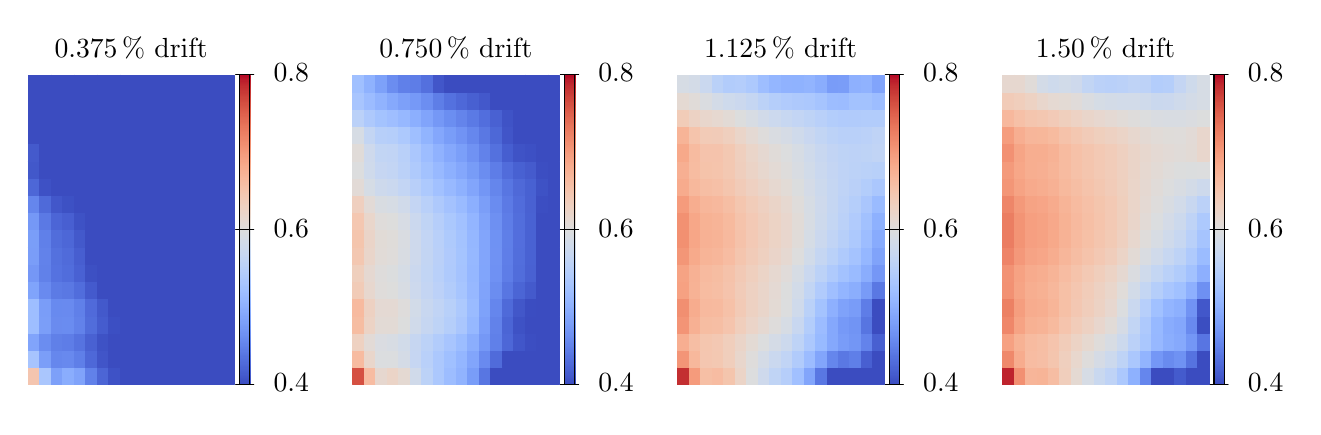
\begin{tikzpicture}[gnuplot]
%% generated with GNUPLOT 5.2p6 (Lua 5.3; terminal rev. Nov 2018, script rev. 107)
%% 03/17/2019 20:39:52
\path (0.000,0.000) rectangle (15.000,4.500);
\gpcolor{color=gp lt color border}
\node[gp node center] at (1.312,4.527) {\SI{0.375}{\percent} drift};
\gpfill{rgb color={0.957,0.774,0.685}} (0.000,0.282)--(0.000,0.501)--(0.146,0.501)--(0.146,0.282)--cycle;
\gpfill{rgb color={0.665,0.778,0.994}} (0.146,0.282)--(0.146,0.501)--(0.292,0.501)--(0.292,0.282)--cycle;
\gpfill{rgb color={0.653,0.770,0.996}} (0.000,0.501)--(0.000,0.719)--(0.146,0.719)--(0.146,0.501)--cycle;
\gpfill{rgb color={0.481,0.619,0.974}} (0.146,0.501)--(0.146,0.719)--(0.292,0.719)--(0.292,0.501)--cycle;
\gpfill{rgb color={0.504,0.643,0.983}} (0.000,0.719)--(0.000,0.938)--(0.146,0.938)--(0.146,0.719)--cycle;
\gpfill{rgb color={0.420,0.553,0.943}} (0.146,0.719)--(0.146,0.938)--(0.292,0.938)--(0.292,0.719)--cycle;
\gpfill{rgb color={0.619,0.744,1.000}} (0.000,0.938)--(0.000,1.157)--(0.146,1.157)--(0.146,0.938)--cycle;
\gpfill{rgb color={0.481,0.619,0.974}} (0.146,0.938)--(0.146,1.157)--(0.292,1.157)--(0.292,0.938)--cycle;
\gpfill{rgb color={0.618,0.744,1.000}} (0.000,1.157)--(0.000,1.376)--(0.146,1.376)--(0.146,1.157)--cycle;
\gpfill{rgb color={0.477,0.616,0.973}} (0.146,1.157)--(0.146,1.376)--(0.292,1.376)--(0.292,1.157)--cycle;
\gpfill{rgb color={0.503,0.642,0.983}} (0.000,1.376)--(0.000,1.594)--(0.146,1.594)--(0.146,1.376)--cycle;
\gpfill{rgb color={0.411,0.542,0.937}} (0.146,1.376)--(0.146,1.594)--(0.292,1.594)--(0.292,1.376)--cycle;
\gpfill{rgb color={0.457,0.594,0.963}} (0.000,1.594)--(0.000,1.813)--(0.146,1.813)--(0.146,1.594)--cycle;
\gpfill{rgb color={0.380,0.506,0.915}} (0.146,1.594)--(0.146,1.813)--(0.292,1.813)--(0.292,1.594)--cycle;
\gpfill{rgb color={0.479,0.617,0.973}} (0.000,1.813)--(0.000,2.032)--(0.146,2.032)--(0.146,1.813)--cycle;
\gpfill{rgb color={0.384,0.511,0.918}} (0.146,1.813)--(0.146,2.032)--(0.292,2.032)--(0.292,1.813)--cycle;
\gpfill{rgb color={0.479,0.618,0.974}} (0.000,2.032)--(0.000,2.250)--(0.146,2.250)--(0.146,2.032)--cycle;
\gpfill{rgb color={0.376,0.501,0.912}} (0.146,2.032)--(0.146,2.250)--(0.292,2.250)--(0.292,2.032)--cycle;
\gpfill{rgb color={0.458,0.595,0.964}} (0.000,2.250)--(0.000,2.468)--(0.146,2.468)--(0.146,2.250)--cycle;
\gpfill{rgb color={0.355,0.475,0.895}} (0.146,2.250)--(0.146,2.468)--(0.292,2.468)--(0.292,2.250)--cycle;
\gpfill{rgb color={0.398,0.527,0.928}} (0.000,2.468)--(0.000,2.687)--(0.146,2.687)--(0.146,2.468)--cycle;
\gpfill{rgb color={0.310,0.415,0.851}} (0.146,2.468)--(0.146,2.687)--(0.292,2.687)--(0.292,2.468)--cycle;
\gpfill{rgb color={0.302,0.404,0.843}} (0.000,2.687)--(0.000,2.906)--(0.146,2.906)--(0.146,2.687)--cycle;
\gpfill{rgb color={0.242,0.318,0.771}} (0.146,2.687)--(0.146,2.906)--(0.292,2.906)--(0.292,2.687)--cycle;
\gpfill{rgb color={0.260,0.344,0.793}} (0.000,2.906)--(0.000,3.124)--(0.146,3.124)--(0.146,2.906)--cycle;
\gpfill{rgb color={0.230,0.299,0.754}} (0.146,2.906)--(0.146,3.124)--(0.292,3.124)--(0.292,2.906)--cycle;
\gpfill{rgb color={0.265,0.351,0.799}} (0.000,3.124)--(0.000,3.343)--(0.146,3.343)--(0.146,3.124)--cycle;
\gpfill{rgb color={0.230,0.299,0.754}} (0.146,3.124)--(0.146,3.343)--(0.292,3.343)--(0.292,3.124)--cycle;
\gpfill{rgb color={0.230,0.299,0.754}} (0.000,3.343)--(0.000,3.562)--(0.146,3.562)--(0.146,3.343)--cycle;
\gpfill{rgb color={0.230,0.299,0.754}} (0.146,3.343)--(0.146,3.562)--(0.292,3.562)--(0.292,3.343)--cycle;
\gpfill{rgb color={0.230,0.299,0.754}} (0.000,3.562)--(0.000,3.781)--(0.146,3.781)--(0.146,3.562)--cycle;
\gpfill{rgb color={0.230,0.299,0.754}} (0.146,3.562)--(0.146,3.781)--(0.292,3.781)--(0.292,3.562)--cycle;
\gpfill{rgb color={0.230,0.299,0.754}} (0.000,3.781)--(0.000,3.999)--(0.146,3.999)--(0.146,3.781)--cycle;
\gpfill{rgb color={0.230,0.299,0.754}} (0.146,3.781)--(0.146,3.999)--(0.292,3.999)--(0.292,3.781)--cycle;
\gpfill{rgb color={0.230,0.299,0.754}} (0.000,3.999)--(0.000,4.218)--(0.146,4.218)--(0.146,3.999)--cycle;
\gpfill{rgb color={0.230,0.299,0.754}} (0.146,3.999)--(0.146,4.218)--(0.292,4.218)--(0.292,3.999)--cycle;
\gpfill{rgb color={0.491,0.629,0.978}} (0.292,0.282)--(0.292,0.501)--(0.438,0.501)--(0.438,0.282)--cycle;
\gpfill{rgb color={0.540,0.677,0.993}} (0.438,0.282)--(0.438,0.501)--(0.583,0.501)--(0.583,0.282)--cycle;
\gpfill{rgb color={0.400,0.529,0.930}} (0.292,0.501)--(0.292,0.719)--(0.438,0.719)--(0.438,0.501)--cycle;
\gpfill{rgb color={0.406,0.537,0.934}} (0.438,0.501)--(0.438,0.719)--(0.583,0.719)--(0.583,0.501)--cycle;
\gpfill{rgb color={0.375,0.500,0.911}} (0.292,0.719)--(0.292,0.938)--(0.438,0.938)--(0.438,0.719)--cycle;
\gpfill{rgb color={0.367,0.489,0.904}} (0.438,0.719)--(0.438,0.938)--(0.583,0.938)--(0.583,0.719)--cycle;
\gpfill{rgb color={0.414,0.546,0.939}} (0.292,0.938)--(0.292,1.157)--(0.438,1.157)--(0.438,0.938)--cycle;
\gpfill{rgb color={0.416,0.549,0.940}} (0.438,0.938)--(0.438,1.157)--(0.583,1.157)--(0.583,0.938)--cycle;
\gpfill{rgb color={0.409,0.541,0.936}} (0.292,1.157)--(0.292,1.376)--(0.438,1.376)--(0.438,1.157)--cycle;
\gpfill{rgb color={0.411,0.542,0.937}} (0.438,1.157)--(0.438,1.376)--(0.583,1.376)--(0.583,1.157)--cycle;
\gpfill{rgb color={0.361,0.482,0.900}} (0.292,1.376)--(0.292,1.594)--(0.438,1.594)--(0.438,1.376)--cycle;
\gpfill{rgb color={0.351,0.469,0.891}} (0.438,1.376)--(0.438,1.594)--(0.583,1.594)--(0.583,1.376)--cycle;
\gpfill{rgb color={0.335,0.449,0.877}} (0.292,1.594)--(0.292,1.813)--(0.438,1.813)--(0.438,1.594)--cycle;
\gpfill{rgb color={0.319,0.428,0.861}} (0.438,1.594)--(0.438,1.813)--(0.583,1.813)--(0.583,1.594)--cycle;
\gpfill{rgb color={0.331,0.443,0.872}} (0.292,1.813)--(0.292,2.032)--(0.438,2.032)--(0.438,1.813)--cycle;
\gpfill{rgb color={0.314,0.420,0.855}} (0.438,1.813)--(0.438,2.032)--(0.583,2.032)--(0.583,1.813)--cycle;
\gpfill{rgb color={0.318,0.426,0.860}} (0.292,2.032)--(0.292,2.250)--(0.438,2.250)--(0.438,2.032)--cycle;
\gpfill{rgb color={0.301,0.402,0.842}} (0.438,2.032)--(0.438,2.250)--(0.583,2.250)--(0.583,2.032)--cycle;
\gpfill{rgb color={0.298,0.398,0.839}} (0.292,2.250)--(0.292,2.468)--(0.438,2.468)--(0.438,2.250)--cycle;
\gpfill{rgb color={0.281,0.374,0.819}} (0.438,2.250)--(0.438,2.468)--(0.583,2.468)--(0.583,2.250)--cycle;
\gpfill{rgb color={0.259,0.343,0.793}} (0.292,2.468)--(0.292,2.687)--(0.438,2.687)--(0.438,2.468)--cycle;
\gpfill{rgb color={0.241,0.316,0.770}} (0.438,2.468)--(0.438,2.687)--(0.583,2.687)--(0.583,2.468)--cycle;
\gpfill{rgb color={0.230,0.299,0.754}} (0.292,2.687)--(0.292,2.906)--(0.438,2.906)--(0.438,2.687)--cycle;
\gpfill{rgb color={0.230,0.299,0.754}} (0.438,2.687)--(0.438,2.906)--(0.583,2.906)--(0.583,2.687)--cycle;
\gpfill{rgb color={0.230,0.299,0.754}} (0.292,2.906)--(0.292,3.124)--(0.438,3.124)--(0.438,2.906)--cycle;
\gpfill{rgb color={0.230,0.299,0.754}} (0.438,2.906)--(0.438,3.124)--(0.583,3.124)--(0.583,2.906)--cycle;
\gpfill{rgb color={0.230,0.299,0.754}} (0.292,3.124)--(0.292,3.343)--(0.438,3.343)--(0.438,3.124)--cycle;
\gpfill{rgb color={0.230,0.299,0.754}} (0.438,3.124)--(0.438,3.343)--(0.583,3.343)--(0.583,3.124)--cycle;
\gpfill{rgb color={0.230,0.299,0.754}} (0.292,3.343)--(0.292,3.562)--(0.438,3.562)--(0.438,3.343)--cycle;
\gpfill{rgb color={0.230,0.299,0.754}} (0.438,3.343)--(0.438,3.562)--(0.583,3.562)--(0.583,3.343)--cycle;
\gpfill{rgb color={0.230,0.299,0.754}} (0.292,3.562)--(0.292,3.781)--(0.438,3.781)--(0.438,3.562)--cycle;
\gpfill{rgb color={0.230,0.299,0.754}} (0.438,3.562)--(0.438,3.781)--(0.583,3.781)--(0.583,3.562)--cycle;
\gpfill{rgb color={0.230,0.299,0.754}} (0.292,3.781)--(0.292,3.999)--(0.438,3.999)--(0.438,3.781)--cycle;
\gpfill{rgb color={0.230,0.299,0.754}} (0.438,3.781)--(0.438,3.999)--(0.583,3.999)--(0.583,3.781)--cycle;
\gpfill{rgb color={0.230,0.299,0.754}} (0.292,3.999)--(0.292,4.218)--(0.438,4.218)--(0.438,3.999)--cycle;
\gpfill{rgb color={0.230,0.299,0.754}} (0.438,3.999)--(0.438,4.218)--(0.583,4.218)--(0.583,3.999)--cycle;
\gpfill{rgb color={0.502,0.641,0.982}} (0.583,0.282)--(0.583,0.501)--(0.729,0.501)--(0.729,0.282)--cycle;
\gpfill{rgb color={0.380,0.506,0.915}} (0.729,0.282)--(0.729,0.501)--(0.875,0.501)--(0.875,0.282)--cycle;
\gpfill{rgb color={0.374,0.498,0.910}} (0.583,0.501)--(0.583,0.719)--(0.729,0.719)--(0.729,0.501)--cycle;
\gpfill{rgb color={0.306,0.409,0.847}} (0.729,0.501)--(0.729,0.719)--(0.875,0.719)--(0.875,0.501)--cycle;
\gpfill{rgb color={0.336,0.450,0.878}} (0.583,0.719)--(0.583,0.938)--(0.729,0.938)--(0.729,0.719)--cycle;
\gpfill{rgb color={0.286,0.381,0.825}} (0.729,0.719)--(0.729,0.938)--(0.875,0.938)--(0.875,0.719)--cycle;
\gpfill{rgb color={0.383,0.510,0.918}} (0.583,0.938)--(0.583,1.157)--(0.729,1.157)--(0.729,0.938)--cycle;
\gpfill{rgb color={0.318,0.426,0.860}} (0.729,0.938)--(0.729,1.157)--(0.875,1.157)--(0.875,0.938)--cycle;
\gpfill{rgb color={0.377,0.502,0.913}} (0.583,1.157)--(0.583,1.376)--(0.729,1.376)--(0.729,1.157)--cycle;
\gpfill{rgb color={0.312,0.417,0.853}} (0.729,1.157)--(0.729,1.376)--(0.875,1.376)--(0.875,1.157)--cycle;
\gpfill{rgb color={0.319,0.427,0.861}} (0.583,1.376)--(0.583,1.594)--(0.729,1.594)--(0.729,1.376)--cycle;
\gpfill{rgb color={0.267,0.354,0.802}} (0.729,1.376)--(0.729,1.594)--(0.875,1.594)--(0.875,1.376)--cycle;
\gpfill{rgb color={0.287,0.382,0.826}} (0.583,1.594)--(0.583,1.813)--(0.729,1.813)--(0.729,1.594)--cycle;
\gpfill{rgb color={0.238,0.312,0.765}} (0.729,1.594)--(0.729,1.813)--(0.875,1.813)--(0.875,1.594)--cycle;
\gpfill{rgb color={0.278,0.370,0.815}} (0.583,1.813)--(0.583,2.032)--(0.729,2.032)--(0.729,1.813)--cycle;
\gpfill{rgb color={0.230,0.299,0.754}} (0.729,1.813)--(0.729,2.032)--(0.875,2.032)--(0.875,1.813)--cycle;
\gpfill{rgb color={0.264,0.349,0.798}} (0.583,2.032)--(0.583,2.250)--(0.729,2.250)--(0.729,2.032)--cycle;
\gpfill{rgb color={0.230,0.299,0.754}} (0.729,2.032)--(0.729,2.250)--(0.875,2.250)--(0.875,2.032)--cycle;
\gpfill{rgb color={0.244,0.321,0.774}} (0.583,2.250)--(0.583,2.468)--(0.729,2.468)--(0.729,2.250)--cycle;
\gpfill{rgb color={0.230,0.299,0.754}} (0.729,2.250)--(0.729,2.468)--(0.875,2.468)--(0.875,2.250)--cycle;
\gpfill{rgb color={0.230,0.299,0.754}} (0.583,2.468)--(0.583,2.687)--(0.729,2.687)--(0.729,2.468)--cycle;
\gpfill{rgb color={0.230,0.299,0.754}} (0.729,2.468)--(0.729,2.687)--(0.875,2.687)--(0.875,2.468)--cycle;
\gpfill{rgb color={0.230,0.299,0.754}} (0.583,2.687)--(0.583,2.906)--(0.729,2.906)--(0.729,2.687)--cycle;
\gpfill{rgb color={0.230,0.299,0.754}} (0.729,2.687)--(0.729,2.906)--(0.875,2.906)--(0.875,2.687)--cycle;
\gpfill{rgb color={0.230,0.299,0.754}} (0.583,2.906)--(0.583,3.124)--(0.729,3.124)--(0.729,2.906)--cycle;
\gpfill{rgb color={0.230,0.299,0.754}} (0.729,2.906)--(0.729,3.124)--(0.875,3.124)--(0.875,2.906)--cycle;
\gpfill{rgb color={0.230,0.299,0.754}} (0.583,3.124)--(0.583,3.343)--(0.729,3.343)--(0.729,3.124)--cycle;
\gpfill{rgb color={0.230,0.299,0.754}} (0.729,3.124)--(0.729,3.343)--(0.875,3.343)--(0.875,3.124)--cycle;
\gpfill{rgb color={0.230,0.299,0.754}} (0.583,3.343)--(0.583,3.562)--(0.729,3.562)--(0.729,3.343)--cycle;
\gpfill{rgb color={0.230,0.299,0.754}} (0.729,3.343)--(0.729,3.562)--(0.875,3.562)--(0.875,3.343)--cycle;
\gpfill{rgb color={0.230,0.299,0.754}} (0.583,3.562)--(0.583,3.781)--(0.729,3.781)--(0.729,3.562)--cycle;
\gpfill{rgb color={0.230,0.299,0.754}} (0.729,3.562)--(0.729,3.781)--(0.875,3.781)--(0.875,3.562)--cycle;
\gpfill{rgb color={0.230,0.299,0.754}} (0.583,3.781)--(0.583,3.999)--(0.729,3.999)--(0.729,3.781)--cycle;
\gpfill{rgb color={0.230,0.299,0.754}} (0.729,3.781)--(0.729,3.999)--(0.875,3.999)--(0.875,3.781)--cycle;
\gpfill{rgb color={0.230,0.299,0.754}} (0.583,3.999)--(0.583,4.218)--(0.729,4.218)--(0.729,3.999)--cycle;
\gpfill{rgb color={0.230,0.299,0.754}} (0.729,3.999)--(0.729,4.218)--(0.875,4.218)--(0.875,3.999)--cycle;
\gpfill{rgb color={0.297,0.396,0.837}} (0.875,0.282)--(0.875,0.501)--(1.021,0.501)--(1.021,0.282)--cycle;
\gpfill{rgb color={0.245,0.322,0.775}} (1.021,0.282)--(1.021,0.501)--(1.167,0.501)--(1.167,0.282)--cycle;
\gpfill{rgb color={0.253,0.333,0.784}} (0.875,0.501)--(0.875,0.719)--(1.021,0.719)--(1.021,0.501)--cycle;
\gpfill{rgb color={0.230,0.299,0.754}} (1.021,0.501)--(1.021,0.719)--(1.167,0.719)--(1.167,0.501)--cycle;
\gpfill{rgb color={0.244,0.320,0.773}} (0.875,0.719)--(0.875,0.938)--(1.021,0.938)--(1.021,0.719)--cycle;
\gpfill{rgb color={0.230,0.299,0.754}} (1.021,0.719)--(1.021,0.938)--(1.167,0.938)--(1.167,0.719)--cycle;
\gpfill{rgb color={0.270,0.359,0.806}} (0.875,0.938)--(0.875,1.157)--(1.021,1.157)--(1.021,0.938)--cycle;
\gpfill{rgb color={0.236,0.309,0.763}} (1.021,0.938)--(1.021,1.157)--(1.167,1.157)--(1.167,0.938)--cycle;
\gpfill{rgb color={0.263,0.349,0.798}} (0.875,1.157)--(0.875,1.376)--(1.021,1.376)--(1.021,1.157)--cycle;
\gpfill{rgb color={0.230,0.299,0.754}} (1.021,1.157)--(1.021,1.376)--(1.167,1.376)--(1.167,1.157)--cycle;
\gpfill{rgb color={0.230,0.299,0.754}} (0.875,1.376)--(0.875,1.594)--(1.021,1.594)--(1.021,1.376)--cycle;
\gpfill{rgb color={0.230,0.299,0.754}} (1.021,1.376)--(1.021,1.594)--(1.167,1.594)--(1.167,1.376)--cycle;
\gpfill{rgb color={0.230,0.299,0.754}} (0.875,1.594)--(0.875,1.813)--(1.021,1.813)--(1.021,1.594)--cycle;
\gpfill{rgb color={0.230,0.299,0.754}} (1.021,1.594)--(1.021,1.813)--(1.167,1.813)--(1.167,1.594)--cycle;
\gpfill{rgb color={0.230,0.299,0.754}} (0.875,1.813)--(0.875,2.032)--(1.021,2.032)--(1.021,1.813)--cycle;
\gpfill{rgb color={0.230,0.299,0.754}} (1.021,1.813)--(1.021,2.032)--(1.167,2.032)--(1.167,1.813)--cycle;
\gpfill{rgb color={0.230,0.299,0.754}} (0.875,2.032)--(0.875,2.250)--(1.021,2.250)--(1.021,2.032)--cycle;
\gpfill{rgb color={0.230,0.299,0.754}} (1.021,2.032)--(1.021,2.250)--(1.167,2.250)--(1.167,2.032)--cycle;
\gpfill{rgb color={0.230,0.299,0.754}} (0.875,2.250)--(0.875,2.468)--(1.021,2.468)--(1.021,2.250)--cycle;
\gpfill{rgb color={0.230,0.299,0.754}} (1.021,2.250)--(1.021,2.468)--(1.167,2.468)--(1.167,2.250)--cycle;
\gpfill{rgb color={0.230,0.299,0.754}} (0.875,2.468)--(0.875,2.687)--(1.021,2.687)--(1.021,2.468)--cycle;
\gpfill{rgb color={0.230,0.299,0.754}} (1.021,2.468)--(1.021,2.687)--(1.167,2.687)--(1.167,2.468)--cycle;
\gpfill{rgb color={0.230,0.299,0.754}} (0.875,2.687)--(0.875,2.906)--(1.021,2.906)--(1.021,2.687)--cycle;
\gpfill{rgb color={0.230,0.299,0.754}} (1.021,2.687)--(1.021,2.906)--(1.167,2.906)--(1.167,2.687)--cycle;
\gpfill{rgb color={0.230,0.299,0.754}} (0.875,2.906)--(0.875,3.124)--(1.021,3.124)--(1.021,2.906)--cycle;
\gpfill{rgb color={0.230,0.299,0.754}} (1.021,2.906)--(1.021,3.124)--(1.167,3.124)--(1.167,2.906)--cycle;
\gpfill{rgb color={0.230,0.299,0.754}} (0.875,3.124)--(0.875,3.343)--(1.021,3.343)--(1.021,3.124)--cycle;
\gpfill{rgb color={0.230,0.299,0.754}} (1.021,3.124)--(1.021,3.343)--(1.167,3.343)--(1.167,3.124)--cycle;
\gpfill{rgb color={0.230,0.299,0.754}} (0.875,3.343)--(0.875,3.562)--(1.021,3.562)--(1.021,3.343)--cycle;
\gpfill{rgb color={0.230,0.299,0.754}} (1.021,3.343)--(1.021,3.562)--(1.167,3.562)--(1.167,3.343)--cycle;
\gpfill{rgb color={0.230,0.299,0.754}} (0.875,3.562)--(0.875,3.781)--(1.021,3.781)--(1.021,3.562)--cycle;
\gpfill{rgb color={0.230,0.299,0.754}} (1.021,3.562)--(1.021,3.781)--(1.167,3.781)--(1.167,3.562)--cycle;
\gpfill{rgb color={0.230,0.299,0.754}} (0.875,3.781)--(0.875,3.999)--(1.021,3.999)--(1.021,3.781)--cycle;
\gpfill{rgb color={0.230,0.299,0.754}} (1.021,3.781)--(1.021,3.999)--(1.167,3.999)--(1.167,3.781)--cycle;
\gpfill{rgb color={0.230,0.299,0.754}} (0.875,3.999)--(0.875,4.218)--(1.021,4.218)--(1.021,3.999)--cycle;
\gpfill{rgb color={0.230,0.299,0.754}} (1.021,3.999)--(1.021,4.218)--(1.167,4.218)--(1.167,3.999)--cycle;
\gpfill{rgb color={0.230,0.299,0.754}} (1.167,0.282)--(1.167,0.501)--(1.312,0.501)--(1.312,0.282)--cycle;
\gpfill{rgb color={0.230,0.299,0.754}} (1.312,0.282)--(1.312,0.501)--(1.457,0.501)--(1.457,0.282)--cycle;
\gpfill{rgb color={0.230,0.299,0.754}} (1.167,0.501)--(1.167,0.719)--(1.312,0.719)--(1.312,0.501)--cycle;
\gpfill{rgb color={0.230,0.299,0.754}} (1.312,0.501)--(1.312,0.719)--(1.457,0.719)--(1.457,0.501)--cycle;
\gpfill{rgb color={0.230,0.299,0.754}} (1.167,0.719)--(1.167,0.938)--(1.312,0.938)--(1.312,0.719)--cycle;
\gpfill{rgb color={0.230,0.299,0.754}} (1.312,0.719)--(1.312,0.938)--(1.457,0.938)--(1.457,0.719)--cycle;
\gpfill{rgb color={0.230,0.299,0.754}} (1.167,0.938)--(1.167,1.157)--(1.312,1.157)--(1.312,0.938)--cycle;
\gpfill{rgb color={0.230,0.299,0.754}} (1.312,0.938)--(1.312,1.157)--(1.457,1.157)--(1.457,0.938)--cycle;
\gpfill{rgb color={0.230,0.299,0.754}} (1.167,1.157)--(1.167,1.376)--(1.312,1.376)--(1.312,1.157)--cycle;
\gpfill{rgb color={0.230,0.299,0.754}} (1.312,1.157)--(1.312,1.376)--(1.457,1.376)--(1.457,1.157)--cycle;
\gpfill{rgb color={0.230,0.299,0.754}} (1.167,1.376)--(1.167,1.594)--(1.312,1.594)--(1.312,1.376)--cycle;
\gpfill{rgb color={0.230,0.299,0.754}} (1.312,1.376)--(1.312,1.594)--(1.457,1.594)--(1.457,1.376)--cycle;
\gpfill{rgb color={0.230,0.299,0.754}} (1.167,1.594)--(1.167,1.813)--(1.312,1.813)--(1.312,1.594)--cycle;
\gpfill{rgb color={0.230,0.299,0.754}} (1.312,1.594)--(1.312,1.813)--(1.457,1.813)--(1.457,1.594)--cycle;
\gpfill{rgb color={0.230,0.299,0.754}} (1.167,1.813)--(1.167,2.032)--(1.312,2.032)--(1.312,1.813)--cycle;
\gpfill{rgb color={0.230,0.299,0.754}} (1.312,1.813)--(1.312,2.032)--(1.457,2.032)--(1.457,1.813)--cycle;
\gpfill{rgb color={0.230,0.299,0.754}} (1.167,2.032)--(1.167,2.250)--(1.312,2.250)--(1.312,2.032)--cycle;
\gpfill{rgb color={0.230,0.299,0.754}} (1.312,2.032)--(1.312,2.250)--(1.457,2.250)--(1.457,2.032)--cycle;
\gpfill{rgb color={0.230,0.299,0.754}} (1.167,2.250)--(1.167,2.468)--(1.312,2.468)--(1.312,2.250)--cycle;
\gpfill{rgb color={0.230,0.299,0.754}} (1.312,2.250)--(1.312,2.468)--(1.457,2.468)--(1.457,2.250)--cycle;
\gpfill{rgb color={0.230,0.299,0.754}} (1.167,2.468)--(1.167,2.687)--(1.312,2.687)--(1.312,2.468)--cycle;
\gpfill{rgb color={0.230,0.299,0.754}} (1.312,2.468)--(1.312,2.687)--(1.457,2.687)--(1.457,2.468)--cycle;
\gpfill{rgb color={0.230,0.299,0.754}} (1.167,2.687)--(1.167,2.906)--(1.312,2.906)--(1.312,2.687)--cycle;
\gpfill{rgb color={0.230,0.299,0.754}} (1.312,2.687)--(1.312,2.906)--(1.457,2.906)--(1.457,2.687)--cycle;
\gpfill{rgb color={0.230,0.299,0.754}} (1.167,2.906)--(1.167,3.124)--(1.312,3.124)--(1.312,2.906)--cycle;
\gpfill{rgb color={0.230,0.299,0.754}} (1.312,2.906)--(1.312,3.124)--(1.457,3.124)--(1.457,2.906)--cycle;
\gpfill{rgb color={0.230,0.299,0.754}} (1.167,3.124)--(1.167,3.343)--(1.312,3.343)--(1.312,3.124)--cycle;
\gpfill{rgb color={0.230,0.299,0.754}} (1.312,3.124)--(1.312,3.343)--(1.457,3.343)--(1.457,3.124)--cycle;
\gpfill{rgb color={0.230,0.299,0.754}} (1.167,3.343)--(1.167,3.562)--(1.312,3.562)--(1.312,3.343)--cycle;
\gpfill{rgb color={0.230,0.299,0.754}} (1.312,3.343)--(1.312,3.562)--(1.457,3.562)--(1.457,3.343)--cycle;
\gpfill{rgb color={0.230,0.299,0.754}} (1.167,3.562)--(1.167,3.781)--(1.312,3.781)--(1.312,3.562)--cycle;
\gpfill{rgb color={0.230,0.299,0.754}} (1.312,3.562)--(1.312,3.781)--(1.457,3.781)--(1.457,3.562)--cycle;
\gpfill{rgb color={0.230,0.299,0.754}} (1.167,3.781)--(1.167,3.999)--(1.312,3.999)--(1.312,3.781)--cycle;
\gpfill{rgb color={0.230,0.299,0.754}} (1.312,3.781)--(1.312,3.999)--(1.457,3.999)--(1.457,3.781)--cycle;
\gpfill{rgb color={0.230,0.299,0.754}} (1.167,3.999)--(1.167,4.218)--(1.312,4.218)--(1.312,3.999)--cycle;
\gpfill{rgb color={0.230,0.299,0.754}} (1.312,3.999)--(1.312,4.218)--(1.457,4.218)--(1.457,3.999)--cycle;
\gpfill{rgb color={0.230,0.299,0.754}} (1.457,0.282)--(1.457,0.501)--(1.603,0.501)--(1.603,0.282)--cycle;
\gpfill{rgb color={0.230,0.299,0.754}} (1.603,0.282)--(1.603,0.501)--(1.749,0.501)--(1.749,0.282)--cycle;
\gpfill{rgb color={0.230,0.299,0.754}} (1.457,0.501)--(1.457,0.719)--(1.603,0.719)--(1.603,0.501)--cycle;
\gpfill{rgb color={0.230,0.299,0.754}} (1.603,0.501)--(1.603,0.719)--(1.749,0.719)--(1.749,0.501)--cycle;
\gpfill{rgb color={0.230,0.299,0.754}} (1.457,0.719)--(1.457,0.938)--(1.603,0.938)--(1.603,0.719)--cycle;
\gpfill{rgb color={0.230,0.299,0.754}} (1.603,0.719)--(1.603,0.938)--(1.749,0.938)--(1.749,0.719)--cycle;
\gpfill{rgb color={0.230,0.299,0.754}} (1.457,0.938)--(1.457,1.157)--(1.603,1.157)--(1.603,0.938)--cycle;
\gpfill{rgb color={0.230,0.299,0.754}} (1.603,0.938)--(1.603,1.157)--(1.749,1.157)--(1.749,0.938)--cycle;
\gpfill{rgb color={0.230,0.299,0.754}} (1.457,1.157)--(1.457,1.376)--(1.603,1.376)--(1.603,1.157)--cycle;
\gpfill{rgb color={0.230,0.299,0.754}} (1.603,1.157)--(1.603,1.376)--(1.749,1.376)--(1.749,1.157)--cycle;
\gpfill{rgb color={0.230,0.299,0.754}} (1.457,1.376)--(1.457,1.594)--(1.603,1.594)--(1.603,1.376)--cycle;
\gpfill{rgb color={0.230,0.299,0.754}} (1.603,1.376)--(1.603,1.594)--(1.749,1.594)--(1.749,1.376)--cycle;
\gpfill{rgb color={0.230,0.299,0.754}} (1.457,1.594)--(1.457,1.813)--(1.603,1.813)--(1.603,1.594)--cycle;
\gpfill{rgb color={0.230,0.299,0.754}} (1.603,1.594)--(1.603,1.813)--(1.749,1.813)--(1.749,1.594)--cycle;
\gpfill{rgb color={0.230,0.299,0.754}} (1.457,1.813)--(1.457,2.032)--(1.603,2.032)--(1.603,1.813)--cycle;
\gpfill{rgb color={0.230,0.299,0.754}} (1.603,1.813)--(1.603,2.032)--(1.749,2.032)--(1.749,1.813)--cycle;
\gpfill{rgb color={0.230,0.299,0.754}} (1.457,2.032)--(1.457,2.250)--(1.603,2.250)--(1.603,2.032)--cycle;
\gpfill{rgb color={0.230,0.299,0.754}} (1.603,2.032)--(1.603,2.250)--(1.749,2.250)--(1.749,2.032)--cycle;
\gpfill{rgb color={0.230,0.299,0.754}} (1.457,2.250)--(1.457,2.468)--(1.603,2.468)--(1.603,2.250)--cycle;
\gpfill{rgb color={0.230,0.299,0.754}} (1.603,2.250)--(1.603,2.468)--(1.749,2.468)--(1.749,2.250)--cycle;
\gpfill{rgb color={0.230,0.299,0.754}} (1.457,2.468)--(1.457,2.687)--(1.603,2.687)--(1.603,2.468)--cycle;
\gpfill{rgb color={0.230,0.299,0.754}} (1.603,2.468)--(1.603,2.687)--(1.749,2.687)--(1.749,2.468)--cycle;
\gpfill{rgb color={0.230,0.299,0.754}} (1.457,2.687)--(1.457,2.906)--(1.603,2.906)--(1.603,2.687)--cycle;
\gpfill{rgb color={0.230,0.299,0.754}} (1.603,2.687)--(1.603,2.906)--(1.749,2.906)--(1.749,2.687)--cycle;
\gpfill{rgb color={0.230,0.299,0.754}} (1.457,2.906)--(1.457,3.124)--(1.603,3.124)--(1.603,2.906)--cycle;
\gpfill{rgb color={0.230,0.299,0.754}} (1.603,2.906)--(1.603,3.124)--(1.749,3.124)--(1.749,2.906)--cycle;
\gpfill{rgb color={0.230,0.299,0.754}} (1.457,3.124)--(1.457,3.343)--(1.603,3.343)--(1.603,3.124)--cycle;
\gpfill{rgb color={0.230,0.299,0.754}} (1.603,3.124)--(1.603,3.343)--(1.749,3.343)--(1.749,3.124)--cycle;
\gpfill{rgb color={0.230,0.299,0.754}} (1.457,3.343)--(1.457,3.562)--(1.603,3.562)--(1.603,3.343)--cycle;
\gpfill{rgb color={0.230,0.299,0.754}} (1.603,3.343)--(1.603,3.562)--(1.749,3.562)--(1.749,3.343)--cycle;
\gpfill{rgb color={0.230,0.299,0.754}} (1.457,3.562)--(1.457,3.781)--(1.603,3.781)--(1.603,3.562)--cycle;
\gpfill{rgb color={0.230,0.299,0.754}} (1.603,3.562)--(1.603,3.781)--(1.749,3.781)--(1.749,3.562)--cycle;
\gpfill{rgb color={0.230,0.299,0.754}} (1.457,3.781)--(1.457,3.999)--(1.603,3.999)--(1.603,3.781)--cycle;
\gpfill{rgb color={0.230,0.299,0.754}} (1.603,3.781)--(1.603,3.999)--(1.749,3.999)--(1.749,3.781)--cycle;
\gpfill{rgb color={0.230,0.299,0.754}} (1.457,3.999)--(1.457,4.218)--(1.603,4.218)--(1.603,3.999)--cycle;
\gpfill{rgb color={0.230,0.299,0.754}} (1.603,3.999)--(1.603,4.218)--(1.749,4.218)--(1.749,3.999)--cycle;
\gpfill{rgb color={0.230,0.299,0.754}} (1.749,0.282)--(1.749,0.501)--(1.895,0.501)--(1.895,0.282)--cycle;
\gpfill{rgb color={0.230,0.299,0.754}} (1.895,0.282)--(1.895,0.501)--(2.041,0.501)--(2.041,0.282)--cycle;
\gpfill{rgb color={0.230,0.299,0.754}} (1.749,0.501)--(1.749,0.719)--(1.895,0.719)--(1.895,0.501)--cycle;
\gpfill{rgb color={0.230,0.299,0.754}} (1.895,0.501)--(1.895,0.719)--(2.041,0.719)--(2.041,0.501)--cycle;
\gpfill{rgb color={0.230,0.299,0.754}} (1.749,0.719)--(1.749,0.938)--(1.895,0.938)--(1.895,0.719)--cycle;
\gpfill{rgb color={0.230,0.299,0.754}} (1.895,0.719)--(1.895,0.938)--(2.041,0.938)--(2.041,0.719)--cycle;
\gpfill{rgb color={0.230,0.299,0.754}} (1.749,0.938)--(1.749,1.157)--(1.895,1.157)--(1.895,0.938)--cycle;
\gpfill{rgb color={0.230,0.299,0.754}} (1.895,0.938)--(1.895,1.157)--(2.041,1.157)--(2.041,0.938)--cycle;
\gpfill{rgb color={0.230,0.299,0.754}} (1.749,1.157)--(1.749,1.376)--(1.895,1.376)--(1.895,1.157)--cycle;
\gpfill{rgb color={0.230,0.299,0.754}} (1.895,1.157)--(1.895,1.376)--(2.041,1.376)--(2.041,1.157)--cycle;
\gpfill{rgb color={0.230,0.299,0.754}} (1.749,1.376)--(1.749,1.594)--(1.895,1.594)--(1.895,1.376)--cycle;
\gpfill{rgb color={0.230,0.299,0.754}} (1.895,1.376)--(1.895,1.594)--(2.041,1.594)--(2.041,1.376)--cycle;
\gpfill{rgb color={0.230,0.299,0.754}} (1.749,1.594)--(1.749,1.813)--(1.895,1.813)--(1.895,1.594)--cycle;
\gpfill{rgb color={0.230,0.299,0.754}} (1.895,1.594)--(1.895,1.813)--(2.041,1.813)--(2.041,1.594)--cycle;
\gpfill{rgb color={0.230,0.299,0.754}} (1.749,1.813)--(1.749,2.032)--(1.895,2.032)--(1.895,1.813)--cycle;
\gpfill{rgb color={0.230,0.299,0.754}} (1.895,1.813)--(1.895,2.032)--(2.041,2.032)--(2.041,1.813)--cycle;
\gpfill{rgb color={0.230,0.299,0.754}} (1.749,2.032)--(1.749,2.250)--(1.895,2.250)--(1.895,2.032)--cycle;
\gpfill{rgb color={0.230,0.299,0.754}} (1.895,2.032)--(1.895,2.250)--(2.041,2.250)--(2.041,2.032)--cycle;
\gpfill{rgb color={0.230,0.299,0.754}} (1.749,2.250)--(1.749,2.468)--(1.895,2.468)--(1.895,2.250)--cycle;
\gpfill{rgb color={0.230,0.299,0.754}} (1.895,2.250)--(1.895,2.468)--(2.041,2.468)--(2.041,2.250)--cycle;
\gpfill{rgb color={0.230,0.299,0.754}} (1.749,2.468)--(1.749,2.687)--(1.895,2.687)--(1.895,2.468)--cycle;
\gpfill{rgb color={0.230,0.299,0.754}} (1.895,2.468)--(1.895,2.687)--(2.041,2.687)--(2.041,2.468)--cycle;
\gpfill{rgb color={0.230,0.299,0.754}} (1.749,2.687)--(1.749,2.906)--(1.895,2.906)--(1.895,2.687)--cycle;
\gpfill{rgb color={0.230,0.299,0.754}} (1.895,2.687)--(1.895,2.906)--(2.041,2.906)--(2.041,2.687)--cycle;
\gpfill{rgb color={0.230,0.299,0.754}} (1.749,2.906)--(1.749,3.124)--(1.895,3.124)--(1.895,2.906)--cycle;
\gpfill{rgb color={0.230,0.299,0.754}} (1.895,2.906)--(1.895,3.124)--(2.041,3.124)--(2.041,2.906)--cycle;
\gpfill{rgb color={0.230,0.299,0.754}} (1.749,3.124)--(1.749,3.343)--(1.895,3.343)--(1.895,3.124)--cycle;
\gpfill{rgb color={0.230,0.299,0.754}} (1.895,3.124)--(1.895,3.343)--(2.041,3.343)--(2.041,3.124)--cycle;
\gpfill{rgb color={0.230,0.299,0.754}} (1.749,3.343)--(1.749,3.562)--(1.895,3.562)--(1.895,3.343)--cycle;
\gpfill{rgb color={0.230,0.299,0.754}} (1.895,3.343)--(1.895,3.562)--(2.041,3.562)--(2.041,3.343)--cycle;
\gpfill{rgb color={0.230,0.299,0.754}} (1.749,3.562)--(1.749,3.781)--(1.895,3.781)--(1.895,3.562)--cycle;
\gpfill{rgb color={0.230,0.299,0.754}} (1.895,3.562)--(1.895,3.781)--(2.041,3.781)--(2.041,3.562)--cycle;
\gpfill{rgb color={0.230,0.299,0.754}} (1.749,3.781)--(1.749,3.999)--(1.895,3.999)--(1.895,3.781)--cycle;
\gpfill{rgb color={0.230,0.299,0.754}} (1.895,3.781)--(1.895,3.999)--(2.041,3.999)--(2.041,3.781)--cycle;
\gpfill{rgb color={0.230,0.299,0.754}} (1.749,3.999)--(1.749,4.218)--(1.895,4.218)--(1.895,3.999)--cycle;
\gpfill{rgb color={0.230,0.299,0.754}} (1.895,3.999)--(1.895,4.218)--(2.041,4.218)--(2.041,3.999)--cycle;
\gpfill{rgb color={0.230,0.299,0.754}} (2.041,0.282)--(2.041,0.501)--(2.186,0.501)--(2.186,0.282)--cycle;
\gpfill{rgb color={0.230,0.299,0.754}} (2.186,0.282)--(2.186,0.501)--(2.332,0.501)--(2.332,0.282)--cycle;
\gpfill{rgb color={0.230,0.299,0.754}} (2.041,0.501)--(2.041,0.719)--(2.186,0.719)--(2.186,0.501)--cycle;
\gpfill{rgb color={0.230,0.299,0.754}} (2.186,0.501)--(2.186,0.719)--(2.332,0.719)--(2.332,0.501)--cycle;
\gpfill{rgb color={0.230,0.299,0.754}} (2.041,0.719)--(2.041,0.938)--(2.186,0.938)--(2.186,0.719)--cycle;
\gpfill{rgb color={0.230,0.299,0.754}} (2.186,0.719)--(2.186,0.938)--(2.332,0.938)--(2.332,0.719)--cycle;
\gpfill{rgb color={0.230,0.299,0.754}} (2.041,0.938)--(2.041,1.157)--(2.186,1.157)--(2.186,0.938)--cycle;
\gpfill{rgb color={0.230,0.299,0.754}} (2.186,0.938)--(2.186,1.157)--(2.332,1.157)--(2.332,0.938)--cycle;
\gpfill{rgb color={0.230,0.299,0.754}} (2.041,1.157)--(2.041,1.376)--(2.186,1.376)--(2.186,1.157)--cycle;
\gpfill{rgb color={0.230,0.299,0.754}} (2.186,1.157)--(2.186,1.376)--(2.332,1.376)--(2.332,1.157)--cycle;
\gpfill{rgb color={0.230,0.299,0.754}} (2.041,1.376)--(2.041,1.594)--(2.186,1.594)--(2.186,1.376)--cycle;
\gpfill{rgb color={0.230,0.299,0.754}} (2.186,1.376)--(2.186,1.594)--(2.332,1.594)--(2.332,1.376)--cycle;
\gpfill{rgb color={0.230,0.299,0.754}} (2.041,1.594)--(2.041,1.813)--(2.186,1.813)--(2.186,1.594)--cycle;
\gpfill{rgb color={0.230,0.299,0.754}} (2.186,1.594)--(2.186,1.813)--(2.332,1.813)--(2.332,1.594)--cycle;
\gpfill{rgb color={0.230,0.299,0.754}} (2.041,1.813)--(2.041,2.032)--(2.186,2.032)--(2.186,1.813)--cycle;
\gpfill{rgb color={0.230,0.299,0.754}} (2.186,1.813)--(2.186,2.032)--(2.332,2.032)--(2.332,1.813)--cycle;
\gpfill{rgb color={0.230,0.299,0.754}} (2.041,2.032)--(2.041,2.250)--(2.186,2.250)--(2.186,2.032)--cycle;
\gpfill{rgb color={0.230,0.299,0.754}} (2.186,2.032)--(2.186,2.250)--(2.332,2.250)--(2.332,2.032)--cycle;
\gpfill{rgb color={0.230,0.299,0.754}} (2.041,2.250)--(2.041,2.468)--(2.186,2.468)--(2.186,2.250)--cycle;
\gpfill{rgb color={0.230,0.299,0.754}} (2.186,2.250)--(2.186,2.468)--(2.332,2.468)--(2.332,2.250)--cycle;
\gpfill{rgb color={0.230,0.299,0.754}} (2.041,2.468)--(2.041,2.687)--(2.186,2.687)--(2.186,2.468)--cycle;
\gpfill{rgb color={0.230,0.299,0.754}} (2.186,2.468)--(2.186,2.687)--(2.332,2.687)--(2.332,2.468)--cycle;
\gpfill{rgb color={0.230,0.299,0.754}} (2.041,2.687)--(2.041,2.906)--(2.186,2.906)--(2.186,2.687)--cycle;
\gpfill{rgb color={0.230,0.299,0.754}} (2.186,2.687)--(2.186,2.906)--(2.332,2.906)--(2.332,2.687)--cycle;
\gpfill{rgb color={0.230,0.299,0.754}} (2.041,2.906)--(2.041,3.124)--(2.186,3.124)--(2.186,2.906)--cycle;
\gpfill{rgb color={0.230,0.299,0.754}} (2.186,2.906)--(2.186,3.124)--(2.332,3.124)--(2.332,2.906)--cycle;
\gpfill{rgb color={0.230,0.299,0.754}} (2.041,3.124)--(2.041,3.343)--(2.186,3.343)--(2.186,3.124)--cycle;
\gpfill{rgb color={0.230,0.299,0.754}} (2.186,3.124)--(2.186,3.343)--(2.332,3.343)--(2.332,3.124)--cycle;
\gpfill{rgb color={0.230,0.299,0.754}} (2.041,3.343)--(2.041,3.562)--(2.186,3.562)--(2.186,3.343)--cycle;
\gpfill{rgb color={0.230,0.299,0.754}} (2.186,3.343)--(2.186,3.562)--(2.332,3.562)--(2.332,3.343)--cycle;
\gpfill{rgb color={0.230,0.299,0.754}} (2.041,3.562)--(2.041,3.781)--(2.186,3.781)--(2.186,3.562)--cycle;
\gpfill{rgb color={0.230,0.299,0.754}} (2.186,3.562)--(2.186,3.781)--(2.332,3.781)--(2.332,3.562)--cycle;
\gpfill{rgb color={0.230,0.299,0.754}} (2.041,3.781)--(2.041,3.999)--(2.186,3.999)--(2.186,3.781)--cycle;
\gpfill{rgb color={0.230,0.299,0.754}} (2.186,3.781)--(2.186,3.999)--(2.332,3.999)--(2.332,3.781)--cycle;
\gpfill{rgb color={0.230,0.299,0.754}} (2.041,3.999)--(2.041,4.218)--(2.186,4.218)--(2.186,3.999)--cycle;
\gpfill{rgb color={0.230,0.299,0.754}} (2.186,3.999)--(2.186,4.218)--(2.332,4.218)--(2.332,3.999)--cycle;
\gpfill{rgb color={0.230,0.299,0.754}} (2.332,0.282)--(2.332,0.501)--(2.478,0.501)--(2.478,0.282)--cycle;
\gpfill{rgb color={0.230,0.299,0.754}} (2.478,0.282)--(2.478,0.501)--(2.624,0.501)--(2.624,0.282)--cycle;
\gpfill{rgb color={0.230,0.299,0.754}} (2.332,0.501)--(2.332,0.719)--(2.478,0.719)--(2.478,0.501)--cycle;
\gpfill{rgb color={0.230,0.299,0.754}} (2.478,0.501)--(2.478,0.719)--(2.624,0.719)--(2.624,0.501)--cycle;
\gpfill{rgb color={0.230,0.299,0.754}} (2.332,0.719)--(2.332,0.938)--(2.478,0.938)--(2.478,0.719)--cycle;
\gpfill{rgb color={0.230,0.299,0.754}} (2.478,0.719)--(2.478,0.938)--(2.624,0.938)--(2.624,0.719)--cycle;
\gpfill{rgb color={0.230,0.299,0.754}} (2.332,0.938)--(2.332,1.157)--(2.478,1.157)--(2.478,0.938)--cycle;
\gpfill{rgb color={0.230,0.299,0.754}} (2.478,0.938)--(2.478,1.157)--(2.624,1.157)--(2.624,0.938)--cycle;
\gpfill{rgb color={0.230,0.299,0.754}} (2.332,1.157)--(2.332,1.376)--(2.478,1.376)--(2.478,1.157)--cycle;
\gpfill{rgb color={0.230,0.299,0.754}} (2.478,1.157)--(2.478,1.376)--(2.624,1.376)--(2.624,1.157)--cycle;
\gpfill{rgb color={0.230,0.299,0.754}} (2.332,1.376)--(2.332,1.594)--(2.478,1.594)--(2.478,1.376)--cycle;
\gpfill{rgb color={0.230,0.299,0.754}} (2.478,1.376)--(2.478,1.594)--(2.624,1.594)--(2.624,1.376)--cycle;
\gpfill{rgb color={0.230,0.299,0.754}} (2.332,1.594)--(2.332,1.813)--(2.478,1.813)--(2.478,1.594)--cycle;
\gpfill{rgb color={0.230,0.299,0.754}} (2.478,1.594)--(2.478,1.813)--(2.624,1.813)--(2.624,1.594)--cycle;
\gpfill{rgb color={0.230,0.299,0.754}} (2.332,1.813)--(2.332,2.032)--(2.478,2.032)--(2.478,1.813)--cycle;
\gpfill{rgb color={0.230,0.299,0.754}} (2.478,1.813)--(2.478,2.032)--(2.624,2.032)--(2.624,1.813)--cycle;
\gpfill{rgb color={0.230,0.299,0.754}} (2.332,2.032)--(2.332,2.250)--(2.478,2.250)--(2.478,2.032)--cycle;
\gpfill{rgb color={0.230,0.299,0.754}} (2.478,2.032)--(2.478,2.250)--(2.624,2.250)--(2.624,2.032)--cycle;
\gpfill{rgb color={0.230,0.299,0.754}} (2.332,2.250)--(2.332,2.468)--(2.478,2.468)--(2.478,2.250)--cycle;
\gpfill{rgb color={0.230,0.299,0.754}} (2.478,2.250)--(2.478,2.468)--(2.624,2.468)--(2.624,2.250)--cycle;
\gpfill{rgb color={0.230,0.299,0.754}} (2.332,2.468)--(2.332,2.687)--(2.478,2.687)--(2.478,2.468)--cycle;
\gpfill{rgb color={0.230,0.299,0.754}} (2.478,2.468)--(2.478,2.687)--(2.624,2.687)--(2.624,2.468)--cycle;
\gpfill{rgb color={0.230,0.299,0.754}} (2.332,2.687)--(2.332,2.906)--(2.478,2.906)--(2.478,2.687)--cycle;
\gpfill{rgb color={0.230,0.299,0.754}} (2.478,2.687)--(2.478,2.906)--(2.624,2.906)--(2.624,2.687)--cycle;
\gpfill{rgb color={0.230,0.299,0.754}} (2.332,2.906)--(2.332,3.124)--(2.478,3.124)--(2.478,2.906)--cycle;
\gpfill{rgb color={0.230,0.299,0.754}} (2.478,2.906)--(2.478,3.124)--(2.624,3.124)--(2.624,2.906)--cycle;
\gpfill{rgb color={0.230,0.299,0.754}} (2.332,3.124)--(2.332,3.343)--(2.478,3.343)--(2.478,3.124)--cycle;
\gpfill{rgb color={0.230,0.299,0.754}} (2.478,3.124)--(2.478,3.343)--(2.624,3.343)--(2.624,3.124)--cycle;
\gpfill{rgb color={0.230,0.299,0.754}} (2.332,3.343)--(2.332,3.562)--(2.478,3.562)--(2.478,3.343)--cycle;
\gpfill{rgb color={0.230,0.299,0.754}} (2.478,3.343)--(2.478,3.562)--(2.624,3.562)--(2.624,3.343)--cycle;
\gpfill{rgb color={0.230,0.299,0.754}} (2.332,3.562)--(2.332,3.781)--(2.478,3.781)--(2.478,3.562)--cycle;
\gpfill{rgb color={0.230,0.299,0.754}} (2.478,3.562)--(2.478,3.781)--(2.624,3.781)--(2.624,3.562)--cycle;
\gpfill{rgb color={0.230,0.299,0.754}} (2.332,3.781)--(2.332,3.999)--(2.478,3.999)--(2.478,3.781)--cycle;
\gpfill{rgb color={0.230,0.299,0.754}} (2.478,3.781)--(2.478,3.999)--(2.624,3.999)--(2.624,3.781)--cycle;
\gpfill{rgb color={0.230,0.299,0.754}} (2.332,3.999)--(2.332,4.218)--(2.478,4.218)--(2.478,3.999)--cycle;
\gpfill{rgb color={0.230,0.299,0.754}} (2.478,3.999)--(2.478,4.218)--(2.624,4.218)--(2.624,3.999)--cycle;
\gpfill{rgb color={0.230,0.299,0.754}} (2.690,0.282)--(2.821,0.282)--(2.821,0.298)--(2.690,0.298)--cycle;
\gpfill{rgb color={0.234,0.306,0.760}} (2.690,0.297)--(2.821,0.297)--(2.821,0.313)--(2.690,0.313)--cycle;
\gpfill{rgb color={0.239,0.312,0.766}} (2.690,0.312)--(2.821,0.312)--(2.821,0.329)--(2.690,0.329)--cycle;
\gpfill{rgb color={0.244,0.320,0.772}} (2.690,0.328)--(2.821,0.328)--(2.821,0.344)--(2.690,0.344)--cycle;
\gpfill{rgb color={0.248,0.326,0.778}} (2.690,0.343)--(2.821,0.343)--(2.821,0.359)--(2.690,0.359)--cycle;
\gpfill{rgb color={0.252,0.333,0.784}} (2.690,0.358)--(2.821,0.358)--(2.821,0.375)--(2.690,0.375)--cycle;
\gpfill{rgb color={0.257,0.340,0.790}} (2.690,0.374)--(2.821,0.374)--(2.821,0.390)--(2.690,0.390)--cycle;
\gpfill{rgb color={0.262,0.347,0.796}} (2.690,0.389)--(2.821,0.389)--(2.821,0.406)--(2.690,0.406)--cycle;
\gpfill{rgb color={0.267,0.354,0.802}} (2.690,0.405)--(2.821,0.405)--(2.821,0.421)--(2.690,0.421)--cycle;
\gpfill{rgb color={0.271,0.360,0.807}} (2.690,0.420)--(2.821,0.420)--(2.821,0.436)--(2.690,0.436)--cycle;
\gpfill{rgb color={0.276,0.367,0.813}} (2.690,0.435)--(2.821,0.435)--(2.821,0.452)--(2.690,0.452)--cycle;
\gpfill{rgb color={0.280,0.374,0.819}} (2.690,0.451)--(2.821,0.451)--(2.821,0.467)--(2.690,0.467)--cycle;
\gpfill{rgb color={0.285,0.380,0.824}} (2.690,0.466)--(2.821,0.466)--(2.821,0.482)--(2.690,0.482)--cycle;
\gpfill{rgb color={0.290,0.387,0.829}} (2.690,0.481)--(2.821,0.481)--(2.821,0.498)--(2.690,0.498)--cycle;
\gpfill{rgb color={0.295,0.394,0.835}} (2.690,0.497)--(2.821,0.497)--(2.821,0.513)--(2.690,0.513)--cycle;
\gpfill{rgb color={0.299,0.400,0.840}} (2.690,0.512)--(2.821,0.512)--(2.821,0.529)--(2.690,0.529)--cycle;
\gpfill{rgb color={0.304,0.407,0.845}} (2.690,0.528)--(2.821,0.528)--(2.821,0.544)--(2.690,0.544)--cycle;
\gpfill{rgb color={0.309,0.413,0.850}} (2.690,0.543)--(2.821,0.543)--(2.821,0.559)--(2.690,0.559)--cycle;
\gpfill{rgb color={0.314,0.420,0.855}} (2.690,0.558)--(2.821,0.558)--(2.821,0.575)--(2.690,0.575)--cycle;
\gpfill{rgb color={0.319,0.427,0.860}} (2.690,0.574)--(2.821,0.574)--(2.821,0.590)--(2.690,0.590)--cycle;
\gpfill{rgb color={0.323,0.433,0.865}} (2.690,0.589)--(2.821,0.589)--(2.821,0.605)--(2.690,0.605)--cycle;
\gpfill{rgb color={0.328,0.439,0.870}} (2.690,0.604)--(2.821,0.604)--(2.821,0.621)--(2.690,0.621)--cycle;
\gpfill{rgb color={0.333,0.446,0.875}} (2.690,0.620)--(2.821,0.620)--(2.821,0.636)--(2.690,0.636)--cycle;
\gpfill{rgb color={0.338,0.452,0.879}} (2.690,0.635)--(2.821,0.635)--(2.821,0.652)--(2.690,0.652)--cycle;
\gpfill{rgb color={0.343,0.459,0.884}} (2.690,0.651)--(2.821,0.651)--(2.821,0.667)--(2.690,0.667)--cycle;
\gpfill{rgb color={0.348,0.465,0.888}} (2.690,0.666)--(2.821,0.666)--(2.821,0.682)--(2.690,0.682)--cycle;
\gpfill{rgb color={0.353,0.472,0.893}} (2.690,0.681)--(2.821,0.681)--(2.821,0.698)--(2.690,0.698)--cycle;
\gpfill{rgb color={0.358,0.478,0.897}} (2.690,0.697)--(2.821,0.697)--(2.821,0.713)--(2.690,0.713)--cycle;
\gpfill{rgb color={0.363,0.485,0.901}} (2.690,0.712)--(2.821,0.712)--(2.821,0.728)--(2.690,0.728)--cycle;
\gpfill{rgb color={0.368,0.491,0.905}} (2.690,0.727)--(2.821,0.727)--(2.821,0.744)--(2.690,0.744)--cycle;
\gpfill{rgb color={0.373,0.497,0.910}} (2.690,0.743)--(2.821,0.743)--(2.821,0.759)--(2.690,0.759)--cycle;
\gpfill{rgb color={0.378,0.503,0.914}} (2.690,0.758)--(2.821,0.758)--(2.821,0.775)--(2.690,0.775)--cycle;
\gpfill{rgb color={0.383,0.510,0.918}} (2.690,0.774)--(2.821,0.774)--(2.821,0.790)--(2.690,0.790)--cycle;
\gpfill{rgb color={0.388,0.516,0.921}} (2.690,0.789)--(2.821,0.789)--(2.821,0.805)--(2.690,0.805)--cycle;
\gpfill{rgb color={0.393,0.522,0.925}} (2.690,0.804)--(2.821,0.804)--(2.821,0.821)--(2.690,0.821)--cycle;
\gpfill{rgb color={0.399,0.528,0.929}} (2.690,0.820)--(2.821,0.820)--(2.821,0.836)--(2.690,0.836)--cycle;
\gpfill{rgb color={0.404,0.534,0.932}} (2.690,0.835)--(2.821,0.835)--(2.821,0.851)--(2.690,0.851)--cycle;
\gpfill{rgb color={0.409,0.540,0.936}} (2.690,0.850)--(2.821,0.850)--(2.821,0.867)--(2.690,0.867)--cycle;
\gpfill{rgb color={0.414,0.546,0.939}} (2.690,0.866)--(2.821,0.866)--(2.821,0.882)--(2.690,0.882)--cycle;
\gpfill{rgb color={0.419,0.552,0.942}} (2.690,0.881)--(2.821,0.881)--(2.821,0.898)--(2.690,0.898)--cycle;
\gpfill{rgb color={0.425,0.559,0.946}} (2.690,0.897)--(2.821,0.897)--(2.821,0.913)--(2.690,0.913)--cycle;
\gpfill{rgb color={0.430,0.564,0.949}} (2.690,0.912)--(2.821,0.912)--(2.821,0.928)--(2.690,0.928)--cycle;
\gpfill{rgb color={0.435,0.570,0.952}} (2.690,0.927)--(2.821,0.927)--(2.821,0.944)--(2.690,0.944)--cycle;
\gpfill{rgb color={0.440,0.576,0.955}} (2.690,0.943)--(2.821,0.943)--(2.821,0.959)--(2.690,0.959)--cycle;
\gpfill{rgb color={0.446,0.582,0.958}} (2.690,0.958)--(2.821,0.958)--(2.821,0.974)--(2.690,0.974)--cycle;
\gpfill{rgb color={0.451,0.587,0.960}} (2.690,0.973)--(2.821,0.973)--(2.821,0.990)--(2.690,0.990)--cycle;
\gpfill{rgb color={0.456,0.593,0.963}} (2.690,0.989)--(2.821,0.989)--(2.821,1.005)--(2.690,1.005)--cycle;
\gpfill{rgb color={0.461,0.599,0.966}} (2.690,1.004)--(2.821,1.004)--(2.821,1.021)--(2.690,1.021)--cycle;
\gpfill{rgb color={0.467,0.605,0.968}} (2.690,1.020)--(2.821,1.020)--(2.821,1.036)--(2.690,1.036)--cycle;
\gpfill{rgb color={0.472,0.610,0.971}} (2.690,1.035)--(2.821,1.035)--(2.821,1.051)--(2.690,1.051)--cycle;
\gpfill{rgb color={0.477,0.616,0.973}} (2.690,1.050)--(2.821,1.050)--(2.821,1.067)--(2.690,1.067)--cycle;
\gpfill{rgb color={0.483,0.622,0.975}} (2.690,1.066)--(2.821,1.066)--(2.821,1.082)--(2.690,1.082)--cycle;
\gpfill{rgb color={0.488,0.627,0.977}} (2.690,1.081)--(2.821,1.081)--(2.821,1.097)--(2.690,1.097)--cycle;
\gpfill{rgb color={0.494,0.632,0.979}} (2.690,1.096)--(2.821,1.096)--(2.821,1.113)--(2.690,1.113)--cycle;
\gpfill{rgb color={0.499,0.638,0.981}} (2.690,1.112)--(2.821,1.112)--(2.821,1.128)--(2.690,1.128)--cycle;
\gpfill{rgb color={0.504,0.643,0.983}} (2.690,1.127)--(2.821,1.127)--(2.821,1.144)--(2.690,1.144)--cycle;
\gpfill{rgb color={0.510,0.649,0.985}} (2.690,1.143)--(2.821,1.143)--(2.821,1.159)--(2.690,1.159)--cycle;
\gpfill{rgb color={0.515,0.654,0.987}} (2.690,1.158)--(2.821,1.158)--(2.821,1.174)--(2.690,1.174)--cycle;
\gpfill{rgb color={0.521,0.659,0.988}} (2.690,1.173)--(2.821,1.173)--(2.821,1.190)--(2.690,1.190)--cycle;
\gpfill{rgb color={0.526,0.664,0.990}} (2.690,1.189)--(2.821,1.189)--(2.821,1.205)--(2.690,1.205)--cycle;
\gpfill{rgb color={0.531,0.669,0.991}} (2.690,1.204)--(2.821,1.204)--(2.821,1.220)--(2.690,1.220)--cycle;
\gpfill{rgb color={0.537,0.674,0.992}} (2.690,1.219)--(2.821,1.219)--(2.821,1.236)--(2.690,1.236)--cycle;
\gpfill{rgb color={0.542,0.679,0.993}} (2.690,1.235)--(2.821,1.235)--(2.821,1.251)--(2.690,1.251)--cycle;
\gpfill{rgb color={0.548,0.684,0.994}} (2.690,1.250)--(2.821,1.250)--(2.821,1.267)--(2.690,1.267)--cycle;
\gpfill{rgb color={0.553,0.689,0.995}} (2.690,1.266)--(2.821,1.266)--(2.821,1.282)--(2.690,1.282)--cycle;
\gpfill{rgb color={0.559,0.694,0.996}} (2.690,1.281)--(2.821,1.281)--(2.821,1.297)--(2.690,1.297)--cycle;
\gpfill{rgb color={0.564,0.699,0.997}} (2.690,1.296)--(2.821,1.296)--(2.821,1.313)--(2.690,1.313)--cycle;
\gpfill{rgb color={0.570,0.704,0.998}} (2.690,1.312)--(2.821,1.312)--(2.821,1.328)--(2.690,1.328)--cycle;
\gpfill{rgb color={0.575,0.708,0.998}} (2.690,1.327)--(2.821,1.327)--(2.821,1.343)--(2.690,1.343)--cycle;
\gpfill{rgb color={0.580,0.713,0.999}} (2.690,1.342)--(2.821,1.342)--(2.821,1.359)--(2.690,1.359)--cycle;
\gpfill{rgb color={0.586,0.717,0.999}} (2.690,1.358)--(2.821,1.358)--(2.821,1.374)--(2.690,1.374)--cycle;
\gpfill{rgb color={0.591,0.722,1.000}} (2.690,1.373)--(2.821,1.373)--(2.821,1.390)--(2.690,1.390)--cycle;
\gpfill{rgb color={0.597,0.726,1.000}} (2.690,1.389)--(2.821,1.389)--(2.821,1.405)--(2.690,1.405)--cycle;
\gpfill{rgb color={0.602,0.731,1.000}} (2.690,1.404)--(2.821,1.404)--(2.821,1.420)--(2.690,1.420)--cycle;
\gpfill{rgb color={0.607,0.735,1.000}} (2.690,1.419)--(2.821,1.419)--(2.821,1.436)--(2.690,1.436)--cycle;
\gpfill{rgb color={0.613,0.739,1.000}} (2.690,1.435)--(2.821,1.435)--(2.821,1.451)--(2.690,1.451)--cycle;
\gpfill{rgb color={0.618,0.744,1.000}} (2.690,1.450)--(2.821,1.450)--(2.821,1.466)--(2.690,1.466)--cycle;
\gpfill{rgb color={0.623,0.748,0.999}} (2.690,1.465)--(2.821,1.465)--(2.821,1.482)--(2.690,1.482)--cycle;
\gpfill{rgb color={0.629,0.752,0.999}} (2.690,1.481)--(2.821,1.481)--(2.821,1.497)--(2.690,1.497)--cycle;
\gpfill{rgb color={0.634,0.756,0.999}} (2.690,1.496)--(2.821,1.496)--(2.821,1.513)--(2.690,1.513)--cycle;
\gpfill{rgb color={0.640,0.760,0.998}} (2.690,1.512)--(2.821,1.512)--(2.821,1.528)--(2.690,1.528)--cycle;
\gpfill{rgb color={0.645,0.764,0.997}} (2.690,1.527)--(2.821,1.527)--(2.821,1.543)--(2.690,1.543)--cycle;
\gpfill{rgb color={0.650,0.767,0.997}} (2.690,1.542)--(2.821,1.542)--(2.821,1.559)--(2.690,1.559)--cycle;
\gpfill{rgb color={0.655,0.771,0.996}} (2.690,1.558)--(2.821,1.558)--(2.821,1.574)--(2.690,1.574)--cycle;
\gpfill{rgb color={0.661,0.775,0.995}} (2.690,1.573)--(2.821,1.573)--(2.821,1.589)--(2.690,1.589)--cycle;
\gpfill{rgb color={0.666,0.778,0.994}} (2.690,1.588)--(2.821,1.588)--(2.821,1.605)--(2.690,1.605)--cycle;
\gpfill{rgb color={0.671,0.782,0.993}} (2.690,1.604)--(2.821,1.604)--(2.821,1.620)--(2.690,1.620)--cycle;
\gpfill{rgb color={0.676,0.786,0.992}} (2.690,1.619)--(2.821,1.619)--(2.821,1.636)--(2.690,1.636)--cycle;
\gpfill{rgb color={0.682,0.789,0.990}} (2.690,1.635)--(2.821,1.635)--(2.821,1.651)--(2.690,1.651)--cycle;
\gpfill{rgb color={0.687,0.792,0.989}} (2.690,1.650)--(2.821,1.650)--(2.821,1.666)--(2.690,1.666)--cycle;
\gpfill{rgb color={0.692,0.796,0.987}} (2.690,1.665)--(2.821,1.665)--(2.821,1.682)--(2.690,1.682)--cycle;
\gpfill{rgb color={0.697,0.799,0.986}} (2.690,1.681)--(2.821,1.681)--(2.821,1.697)--(2.690,1.697)--cycle;
\gpfill{rgb color={0.702,0.802,0.984}} (2.690,1.696)--(2.821,1.696)--(2.821,1.712)--(2.690,1.712)--cycle;
\gpfill{rgb color={0.707,0.805,0.982}} (2.690,1.711)--(2.821,1.711)--(2.821,1.728)--(2.690,1.728)--cycle;
\gpfill{rgb color={0.712,0.808,0.980}} (2.690,1.727)--(2.821,1.727)--(2.821,1.743)--(2.690,1.743)--cycle;
\gpfill{rgb color={0.717,0.811,0.979}} (2.690,1.742)--(2.821,1.742)--(2.821,1.759)--(2.690,1.759)--cycle;
\gpfill{rgb color={0.723,0.814,0.976}} (2.690,1.758)--(2.821,1.758)--(2.821,1.774)--(2.690,1.774)--cycle;
\gpfill{rgb color={0.727,0.817,0.974}} (2.690,1.773)--(2.821,1.773)--(2.821,1.789)--(2.690,1.789)--cycle;
\gpfill{rgb color={0.732,0.820,0.972}} (2.690,1.788)--(2.821,1.788)--(2.821,1.805)--(2.690,1.805)--cycle;
\gpfill{rgb color={0.737,0.822,0.970}} (2.690,1.804)--(2.821,1.804)--(2.821,1.820)--(2.690,1.820)--cycle;
\gpfill{rgb color={0.742,0.825,0.967}} (2.690,1.819)--(2.821,1.819)--(2.821,1.835)--(2.690,1.835)--cycle;
\gpfill{rgb color={0.747,0.827,0.965}} (2.690,1.834)--(2.821,1.834)--(2.821,1.851)--(2.690,1.851)--cycle;
\gpfill{rgb color={0.752,0.830,0.962}} (2.690,1.850)--(2.821,1.850)--(2.821,1.866)--(2.690,1.866)--cycle;
\gpfill{rgb color={0.757,0.832,0.960}} (2.690,1.865)--(2.821,1.865)--(2.821,1.882)--(2.690,1.882)--cycle;
\gpfill{rgb color={0.762,0.834,0.957}} (2.690,1.881)--(2.821,1.881)--(2.821,1.897)--(2.690,1.897)--cycle;
\gpfill{rgb color={0.766,0.837,0.954}} (2.690,1.896)--(2.821,1.896)--(2.821,1.912)--(2.690,1.912)--cycle;
\gpfill{rgb color={0.771,0.839,0.951}} (2.690,1.911)--(2.821,1.911)--(2.821,1.928)--(2.690,1.928)--cycle;
\gpfill{rgb color={0.776,0.841,0.948}} (2.690,1.927)--(2.821,1.927)--(2.821,1.943)--(2.690,1.943)--cycle;
\gpfill{rgb color={0.781,0.843,0.945}} (2.690,1.942)--(2.821,1.942)--(2.821,1.958)--(2.690,1.958)--cycle;
\gpfill{rgb color={0.785,0.845,0.942}} (2.690,1.957)--(2.821,1.957)--(2.821,1.974)--(2.690,1.974)--cycle;
\gpfill{rgb color={0.790,0.846,0.938}} (2.690,1.973)--(2.821,1.973)--(2.821,1.989)--(2.690,1.989)--cycle;
\gpfill{rgb color={0.794,0.848,0.935}} (2.690,1.988)--(2.821,1.988)--(2.821,2.005)--(2.690,2.005)--cycle;
\gpfill{rgb color={0.799,0.850,0.931}} (2.690,2.004)--(2.821,2.004)--(2.821,2.020)--(2.690,2.020)--cycle;
\gpfill{rgb color={0.803,0.851,0.928}} (2.690,2.019)--(2.821,2.019)--(2.821,2.035)--(2.690,2.035)--cycle;
\gpfill{rgb color={0.808,0.853,0.924}} (2.690,2.034)--(2.821,2.034)--(2.821,2.051)--(2.690,2.051)--cycle;
\gpfill{rgb color={0.812,0.854,0.921}} (2.690,2.050)--(2.821,2.050)--(2.821,2.066)--(2.690,2.066)--cycle;
\gpfill{rgb color={0.817,0.856,0.917}} (2.690,2.065)--(2.821,2.065)--(2.821,2.081)--(2.690,2.081)--cycle;
\gpfill{rgb color={0.821,0.857,0.913}} (2.690,2.080)--(2.821,2.080)--(2.821,2.097)--(2.690,2.097)--cycle;
\gpfill{rgb color={0.825,0.858,0.909}} (2.690,2.096)--(2.821,2.096)--(2.821,2.112)--(2.690,2.112)--cycle;
\gpfill{rgb color={0.829,0.859,0.905}} (2.690,2.111)--(2.821,2.111)--(2.821,2.128)--(2.690,2.128)--cycle;
\gpfill{rgb color={0.834,0.860,0.901}} (2.690,2.127)--(2.821,2.127)--(2.821,2.143)--(2.690,2.143)--cycle;
\gpfill{rgb color={0.838,0.861,0.897}} (2.690,2.142)--(2.821,2.142)--(2.821,2.158)--(2.690,2.158)--cycle;
\gpfill{rgb color={0.842,0.862,0.893}} (2.690,2.157)--(2.821,2.157)--(2.821,2.174)--(2.690,2.174)--cycle;
\gpfill{rgb color={0.846,0.863,0.888}} (2.690,2.173)--(2.821,2.173)--(2.821,2.189)--(2.690,2.189)--cycle;
\gpfill{rgb color={0.850,0.863,0.884}} (2.690,2.188)--(2.821,2.188)--(2.821,2.204)--(2.690,2.204)--cycle;
\gpfill{rgb color={0.854,0.864,0.879}} (2.690,2.203)--(2.821,2.203)--(2.821,2.220)--(2.690,2.220)--cycle;
\gpfill{rgb color={0.858,0.865,0.875}} (2.690,2.219)--(2.821,2.219)--(2.821,2.235)--(2.690,2.235)--cycle;
\gpfill{rgb color={0.862,0.865,0.870}} (2.690,2.234)--(2.821,2.234)--(2.821,2.251)--(2.690,2.251)--cycle;
\gpfill{rgb color={0.866,0.865,0.865}} (2.690,2.250)--(2.821,2.250)--(2.821,2.266)--(2.690,2.266)--cycle;
\gpfill{rgb color={0.870,0.864,0.860}} (2.690,2.265)--(2.821,2.265)--(2.821,2.281)--(2.690,2.281)--cycle;
\gpfill{rgb color={0.874,0.862,0.854}} (2.690,2.280)--(2.821,2.280)--(2.821,2.297)--(2.690,2.297)--cycle;
\gpfill{rgb color={0.878,0.860,0.849}} (2.690,2.296)--(2.821,2.296)--(2.821,2.312)--(2.690,2.312)--cycle;
\gpfill{rgb color={0.882,0.858,0.843}} (2.690,2.311)--(2.821,2.311)--(2.821,2.327)--(2.690,2.327)--cycle;
\gpfill{rgb color={0.886,0.856,0.838}} (2.690,2.326)--(2.821,2.326)--(2.821,2.343)--(2.690,2.343)--cycle;
\gpfill{rgb color={0.890,0.853,0.832}} (2.690,2.342)--(2.821,2.342)--(2.821,2.358)--(2.690,2.358)--cycle;
\gpfill{rgb color={0.894,0.851,0.826}} (2.690,2.357)--(2.821,2.357)--(2.821,2.374)--(2.690,2.374)--cycle;
\gpfill{rgb color={0.898,0.849,0.821}} (2.690,2.373)--(2.821,2.373)--(2.821,2.389)--(2.690,2.389)--cycle;
\gpfill{rgb color={0.902,0.846,0.815}} (2.690,2.388)--(2.821,2.388)--(2.821,2.404)--(2.690,2.404)--cycle;
\gpfill{rgb color={0.905,0.844,0.809}} (2.690,2.403)--(2.821,2.403)--(2.821,2.420)--(2.690,2.420)--cycle;
\gpfill{rgb color={0.909,0.841,0.803}} (2.690,2.419)--(2.821,2.419)--(2.821,2.435)--(2.690,2.435)--cycle;
\gpfill{rgb color={0.912,0.839,0.798}} (2.690,2.434)--(2.821,2.434)--(2.821,2.450)--(2.690,2.450)--cycle;
\gpfill{rgb color={0.915,0.836,0.792}} (2.690,2.449)--(2.821,2.449)--(2.821,2.466)--(2.690,2.466)--cycle;
\gpfill{rgb color={0.918,0.833,0.786}} (2.690,2.465)--(2.821,2.465)--(2.821,2.481)--(2.690,2.481)--cycle;
\gpfill{rgb color={0.921,0.830,0.780}} (2.690,2.480)--(2.821,2.480)--(2.821,2.497)--(2.690,2.497)--cycle;
\gpfill{rgb color={0.924,0.827,0.774}} (2.690,2.496)--(2.821,2.496)--(2.821,2.512)--(2.690,2.512)--cycle;
\gpfill{rgb color={0.927,0.824,0.768}} (2.690,2.511)--(2.821,2.511)--(2.821,2.527)--(2.690,2.527)--cycle;
\gpfill{rgb color={0.930,0.821,0.763}} (2.690,2.526)--(2.821,2.526)--(2.821,2.543)--(2.690,2.543)--cycle;
\gpfill{rgb color={0.933,0.818,0.756}} (2.690,2.542)--(2.821,2.542)--(2.821,2.558)--(2.690,2.558)--cycle;
\gpfill{rgb color={0.935,0.815,0.751}} (2.690,2.557)--(2.821,2.557)--(2.821,2.573)--(2.690,2.573)--cycle;
\gpfill{rgb color={0.938,0.811,0.745}} (2.690,2.572)--(2.821,2.572)--(2.821,2.589)--(2.690,2.589)--cycle;
\gpfill{rgb color={0.940,0.808,0.738}} (2.690,2.588)--(2.821,2.588)--(2.821,2.604)--(2.690,2.604)--cycle;
\gpfill{rgb color={0.942,0.804,0.733}} (2.690,2.603)--(2.821,2.603)--(2.821,2.620)--(2.690,2.620)--cycle;
\gpfill{rgb color={0.945,0.801,0.726}} (2.690,2.619)--(2.821,2.619)--(2.821,2.635)--(2.690,2.635)--cycle;
\gpfill{rgb color={0.947,0.797,0.720}} (2.690,2.634)--(2.821,2.634)--(2.821,2.650)--(2.690,2.650)--cycle;
\gpfill{rgb color={0.949,0.794,0.715}} (2.690,2.649)--(2.821,2.649)--(2.821,2.666)--(2.690,2.666)--cycle;
\gpfill{rgb color={0.951,0.790,0.708}} (2.690,2.665)--(2.821,2.665)--(2.821,2.681)--(2.690,2.681)--cycle;
\gpfill{rgb color={0.952,0.786,0.702}} (2.690,2.680)--(2.821,2.680)--(2.821,2.696)--(2.690,2.696)--cycle;
\gpfill{rgb color={0.954,0.782,0.696}} (2.690,2.695)--(2.821,2.695)--(2.821,2.712)--(2.690,2.712)--cycle;
\gpfill{rgb color={0.956,0.778,0.690}} (2.690,2.711)--(2.821,2.711)--(2.821,2.727)--(2.690,2.727)--cycle;
\gpfill{rgb color={0.957,0.774,0.684}} (2.690,2.726)--(2.821,2.726)--(2.821,2.743)--(2.690,2.743)--cycle;
\gpfill{rgb color={0.959,0.769,0.678}} (2.690,2.742)--(2.821,2.742)--(2.821,2.758)--(2.690,2.758)--cycle;
\gpfill{rgb color={0.960,0.765,0.672}} (2.690,2.757)--(2.821,2.757)--(2.821,2.773)--(2.690,2.773)--cycle;
\gpfill{rgb color={0.962,0.761,0.666}} (2.690,2.772)--(2.821,2.772)--(2.821,2.789)--(2.690,2.789)--cycle;
\gpfill{rgb color={0.963,0.757,0.659}} (2.690,2.788)--(2.821,2.788)--(2.821,2.804)--(2.690,2.804)--cycle;
\gpfill{rgb color={0.964,0.752,0.653}} (2.690,2.803)--(2.821,2.803)--(2.821,2.819)--(2.690,2.819)--cycle;
\gpfill{rgb color={0.965,0.748,0.647}} (2.690,2.818)--(2.821,2.818)--(2.821,2.835)--(2.690,2.835)--cycle;
\gpfill{rgb color={0.966,0.743,0.641}} (2.690,2.834)--(2.821,2.834)--(2.821,2.850)--(2.690,2.850)--cycle;
\gpfill{rgb color={0.967,0.739,0.635}} (2.690,2.849)--(2.821,2.849)--(2.821,2.866)--(2.690,2.866)--cycle;
\gpfill{rgb color={0.967,0.734,0.628}} (2.690,2.865)--(2.821,2.865)--(2.821,2.881)--(2.690,2.881)--cycle;
\gpfill{rgb color={0.968,0.729,0.622}} (2.690,2.880)--(2.821,2.880)--(2.821,2.896)--(2.690,2.896)--cycle;
\gpfill{rgb color={0.969,0.724,0.616}} (2.690,2.895)--(2.821,2.895)--(2.821,2.912)--(2.690,2.912)--cycle;
\gpfill{rgb color={0.969,0.719,0.610}} (2.690,2.911)--(2.821,2.911)--(2.821,2.927)--(2.690,2.927)--cycle;
\gpfill{rgb color={0.969,0.715,0.604}} (2.690,2.926)--(2.821,2.926)--(2.821,2.942)--(2.690,2.942)--cycle;
\gpfill{rgb color={0.970,0.710,0.598}} (2.690,2.941)--(2.821,2.941)--(2.821,2.958)--(2.690,2.958)--cycle;
\gpfill{rgb color={0.970,0.704,0.591}} (2.690,2.957)--(2.821,2.957)--(2.821,2.973)--(2.690,2.973)--cycle;
\gpfill{rgb color={0.970,0.699,0.585}} (2.690,2.972)--(2.821,2.972)--(2.821,2.989)--(2.690,2.989)--cycle;
\gpfill{rgb color={0.970,0.694,0.579}} (2.690,2.988)--(2.821,2.988)--(2.821,3.004)--(2.690,3.004)--cycle;
\gpfill{rgb color={0.970,0.689,0.573}} (2.690,3.003)--(2.821,3.003)--(2.821,3.019)--(2.690,3.019)--cycle;
\gpfill{rgb color={0.970,0.684,0.567}} (2.690,3.018)--(2.821,3.018)--(2.821,3.035)--(2.690,3.035)--cycle;
\gpfill{rgb color={0.969,0.678,0.561}} (2.690,3.034)--(2.821,3.034)--(2.821,3.050)--(2.690,3.050)--cycle;
\gpfill{rgb color={0.969,0.673,0.555}} (2.690,3.049)--(2.821,3.049)--(2.821,3.065)--(2.690,3.065)--cycle;
\gpfill{rgb color={0.969,0.667,0.549}} (2.690,3.064)--(2.821,3.064)--(2.821,3.081)--(2.690,3.081)--cycle;
\gpfill{rgb color={0.968,0.661,0.542}} (2.690,3.080)--(2.821,3.080)--(2.821,3.096)--(2.690,3.096)--cycle;
\gpfill{rgb color={0.967,0.656,0.536}} (2.690,3.095)--(2.821,3.095)--(2.821,3.112)--(2.690,3.112)--cycle;
\gpfill{rgb color={0.967,0.650,0.530}} (2.690,3.111)--(2.821,3.111)--(2.821,3.127)--(2.690,3.127)--cycle;
\gpfill{rgb color={0.966,0.644,0.524}} (2.690,3.126)--(2.821,3.126)--(2.821,3.142)--(2.690,3.142)--cycle;
\gpfill{rgb color={0.965,0.639,0.518}} (2.690,3.141)--(2.821,3.141)--(2.821,3.158)--(2.690,3.158)--cycle;
\gpfill{rgb color={0.964,0.633,0.512}} (2.690,3.157)--(2.821,3.157)--(2.821,3.173)--(2.690,3.173)--cycle;
\gpfill{rgb color={0.963,0.627,0.506}} (2.690,3.172)--(2.821,3.172)--(2.821,3.188)--(2.690,3.188)--cycle;
\gpfill{rgb color={0.962,0.621,0.500}} (2.690,3.187)--(2.821,3.187)--(2.821,3.204)--(2.690,3.204)--cycle;
\gpfill{rgb color={0.961,0.615,0.494}} (2.690,3.203)--(2.821,3.203)--(2.821,3.219)--(2.690,3.219)--cycle;
\gpfill{rgb color={0.959,0.609,0.488}} (2.690,3.218)--(2.821,3.218)--(2.821,3.235)--(2.690,3.235)--cycle;
\gpfill{rgb color={0.958,0.602,0.481}} (2.690,3.234)--(2.821,3.234)--(2.821,3.250)--(2.690,3.250)--cycle;
\gpfill{rgb color={0.956,0.596,0.476}} (2.690,3.249)--(2.821,3.249)--(2.821,3.265)--(2.690,3.265)--cycle;
\gpfill{rgb color={0.955,0.590,0.470}} (2.690,3.264)--(2.821,3.264)--(2.821,3.281)--(2.690,3.281)--cycle;
\gpfill{rgb color={0.953,0.584,0.463}} (2.690,3.280)--(2.821,3.280)--(2.821,3.296)--(2.690,3.296)--cycle;
\gpfill{rgb color={0.951,0.578,0.458}} (2.690,3.295)--(2.821,3.295)--(2.821,3.311)--(2.690,3.311)--cycle;
\gpfill{rgb color={0.950,0.571,0.452}} (2.690,3.310)--(2.821,3.310)--(2.821,3.327)--(2.690,3.327)--cycle;
\gpfill{rgb color={0.948,0.565,0.446}} (2.690,3.326)--(2.821,3.326)--(2.821,3.342)--(2.690,3.342)--cycle;
\gpfill{rgb color={0.946,0.558,0.440}} (2.690,3.341)--(2.821,3.341)--(2.821,3.358)--(2.690,3.358)--cycle;
\gpfill{rgb color={0.944,0.551,0.434}} (2.690,3.357)--(2.821,3.357)--(2.821,3.373)--(2.690,3.373)--cycle;
\gpfill{rgb color={0.941,0.545,0.428}} (2.690,3.372)--(2.821,3.372)--(2.821,3.388)--(2.690,3.388)--cycle;
\gpfill{rgb color={0.939,0.538,0.422}} (2.690,3.387)--(2.821,3.387)--(2.821,3.404)--(2.690,3.404)--cycle;
\gpfill{rgb color={0.937,0.531,0.416}} (2.690,3.403)--(2.821,3.403)--(2.821,3.419)--(2.690,3.419)--cycle;
\gpfill{rgb color={0.934,0.525,0.411}} (2.690,3.418)--(2.821,3.418)--(2.821,3.434)--(2.690,3.434)--cycle;
\gpfill{rgb color={0.932,0.518,0.405}} (2.690,3.433)--(2.821,3.433)--(2.821,3.450)--(2.690,3.450)--cycle;
\gpfill{rgb color={0.929,0.511,0.399}} (2.690,3.449)--(2.821,3.449)--(2.821,3.465)--(2.690,3.465)--cycle;
\gpfill{rgb color={0.927,0.504,0.394}} (2.690,3.464)--(2.821,3.464)--(2.821,3.481)--(2.690,3.481)--cycle;
\gpfill{rgb color={0.924,0.497,0.388}} (2.690,3.480)--(2.821,3.480)--(2.821,3.496)--(2.690,3.496)--cycle;
\gpfill{rgb color={0.921,0.490,0.382}} (2.690,3.495)--(2.821,3.495)--(2.821,3.511)--(2.690,3.511)--cycle;
\gpfill{rgb color={0.918,0.483,0.377}} (2.690,3.510)--(2.821,3.510)--(2.821,3.527)--(2.690,3.527)--cycle;
\gpfill{rgb color={0.915,0.476,0.371}} (2.690,3.526)--(2.821,3.526)--(2.821,3.542)--(2.690,3.542)--cycle;
\gpfill{rgb color={0.912,0.469,0.365}} (2.690,3.541)--(2.821,3.541)--(2.821,3.557)--(2.690,3.557)--cycle;
\gpfill{rgb color={0.909,0.462,0.360}} (2.690,3.556)--(2.821,3.556)--(2.821,3.573)--(2.690,3.573)--cycle;
\gpfill{rgb color={0.906,0.454,0.354}} (2.690,3.572)--(2.821,3.572)--(2.821,3.588)--(2.690,3.588)--cycle;
\gpfill{rgb color={0.902,0.447,0.349}} (2.690,3.587)--(2.821,3.587)--(2.821,3.604)--(2.690,3.604)--cycle;
\gpfill{rgb color={0.899,0.439,0.343}} (2.690,3.603)--(2.821,3.603)--(2.821,3.619)--(2.690,3.619)--cycle;
\gpfill{rgb color={0.895,0.432,0.338}} (2.690,3.618)--(2.821,3.618)--(2.821,3.634)--(2.690,3.634)--cycle;
\gpfill{rgb color={0.892,0.424,0.332}} (2.690,3.633)--(2.821,3.633)--(2.821,3.650)--(2.690,3.650)--cycle;
\gpfill{rgb color={0.888,0.417,0.327}} (2.690,3.649)--(2.821,3.649)--(2.821,3.665)--(2.690,3.665)--cycle;
\gpfill{rgb color={0.885,0.409,0.321}} (2.690,3.664)--(2.821,3.664)--(2.821,3.680)--(2.690,3.680)--cycle;
\gpfill{rgb color={0.881,0.402,0.316}} (2.690,3.679)--(2.821,3.679)--(2.821,3.696)--(2.690,3.696)--cycle;
\gpfill{rgb color={0.877,0.394,0.311}} (2.690,3.695)--(2.821,3.695)--(2.821,3.711)--(2.690,3.711)--cycle;
\gpfill{rgb color={0.873,0.386,0.305}} (2.690,3.710)--(2.821,3.710)--(2.821,3.727)--(2.690,3.727)--cycle;
\gpfill{rgb color={0.869,0.378,0.300}} (2.690,3.726)--(2.821,3.726)--(2.821,3.742)--(2.690,3.742)--cycle;
\gpfill{rgb color={0.865,0.370,0.295}} (2.690,3.741)--(2.821,3.741)--(2.821,3.757)--(2.690,3.757)--cycle;
\gpfill{rgb color={0.861,0.362,0.290}} (2.690,3.756)--(2.821,3.756)--(2.821,3.773)--(2.690,3.773)--cycle;
\gpfill{rgb color={0.857,0.354,0.284}} (2.690,3.772)--(2.821,3.772)--(2.821,3.788)--(2.690,3.788)--cycle;
\gpfill{rgb color={0.852,0.346,0.279}} (2.690,3.787)--(2.821,3.787)--(2.821,3.803)--(2.690,3.803)--cycle;
\gpfill{rgb color={0.848,0.338,0.274}} (2.690,3.802)--(2.821,3.802)--(2.821,3.819)--(2.690,3.819)--cycle;
\gpfill{rgb color={0.843,0.329,0.269}} (2.690,3.818)--(2.821,3.818)--(2.821,3.834)--(2.690,3.834)--cycle;
\gpfill{rgb color={0.839,0.321,0.264}} (2.690,3.833)--(2.821,3.833)--(2.821,3.850)--(2.690,3.850)--cycle;
\gpfill{rgb color={0.834,0.312,0.259}} (2.690,3.849)--(2.821,3.849)--(2.821,3.865)--(2.690,3.865)--cycle;
\gpfill{rgb color={0.830,0.304,0.254}} (2.690,3.864)--(2.821,3.864)--(2.821,3.880)--(2.690,3.880)--cycle;
\gpfill{rgb color={0.825,0.296,0.249}} (2.690,3.879)--(2.821,3.879)--(2.821,3.896)--(2.690,3.896)--cycle;
\gpfill{rgb color={0.820,0.286,0.244}} (2.690,3.895)--(2.821,3.895)--(2.821,3.911)--(2.690,3.911)--cycle;
\gpfill{rgb color={0.816,0.278,0.239}} (2.690,3.910)--(2.821,3.910)--(2.821,3.926)--(2.690,3.926)--cycle;
\gpfill{rgb color={0.811,0.269,0.235}} (2.690,3.925)--(2.821,3.925)--(2.821,3.942)--(2.690,3.942)--cycle;
\gpfill{rgb color={0.806,0.260,0.230}} (2.690,3.941)--(2.821,3.941)--(2.821,3.957)--(2.690,3.957)--cycle;
\gpfill{rgb color={0.801,0.250,0.225}} (2.690,3.956)--(2.821,3.956)--(2.821,3.973)--(2.690,3.973)--cycle;
\gpfill{rgb color={0.795,0.241,0.220}} (2.690,3.972)--(2.821,3.972)--(2.821,3.988)--(2.690,3.988)--cycle;
\gpfill{rgb color={0.790,0.231,0.216}} (2.690,3.987)--(2.821,3.987)--(2.821,4.003)--(2.690,4.003)--cycle;
\gpfill{rgb color={0.785,0.222,0.211}} (2.690,4.002)--(2.821,4.002)--(2.821,4.019)--(2.690,4.019)--cycle;
\gpfill{rgb color={0.780,0.211,0.206}} (2.690,4.018)--(2.821,4.018)--(2.821,4.034)--(2.690,4.034)--cycle;
\gpfill{rgb color={0.774,0.201,0.202}} (2.690,4.033)--(2.821,4.033)--(2.821,4.049)--(2.690,4.049)--cycle;
\gpfill{rgb color={0.769,0.191,0.197}} (2.690,4.048)--(2.821,4.048)--(2.821,4.065)--(2.690,4.065)--cycle;
\gpfill{rgb color={0.763,0.180,0.193}} (2.690,4.064)--(2.821,4.064)--(2.821,4.080)--(2.690,4.080)--cycle;
\gpfill{rgb color={0.758,0.169,0.188}} (2.690,4.079)--(2.821,4.079)--(2.821,4.096)--(2.690,4.096)--cycle;
\gpfill{rgb color={0.752,0.156,0.184}} (2.690,4.095)--(2.821,4.095)--(2.821,4.111)--(2.690,4.111)--cycle;
\gpfill{rgb color={0.747,0.144,0.180}} (2.690,4.110)--(2.821,4.110)--(2.821,4.126)--(2.690,4.126)--cycle;
\gpfill{rgb color={0.741,0.132,0.175}} (2.690,4.125)--(2.821,4.125)--(2.821,4.142)--(2.690,4.142)--cycle;
\gpfill{rgb color={0.735,0.117,0.171}} (2.690,4.141)--(2.821,4.141)--(2.821,4.157)--(2.690,4.157)--cycle;
\gpfill{rgb color={0.729,0.103,0.167}} (2.690,4.156)--(2.821,4.156)--(2.821,4.172)--(2.690,4.172)--cycle;
\gpfill{rgb color={0.724,0.086,0.163}} (2.690,4.171)--(2.821,4.171)--(2.821,4.188)--(2.690,4.188)--cycle;
\gpfill{rgb color={0.717,0.066,0.158}} (2.690,4.187)--(2.821,4.187)--(2.821,4.203)--(2.690,4.203)--cycle;
\gpfill{rgb color={0.712,0.043,0.154}} (2.690,4.202)--(2.821,4.202)--(2.821,4.218)--(2.690,4.218)--cycle;
\gpsetlinetype{gp lt border}
\gpsetdashtype{gp dt solid}
\gpsetlinewidth{1.00}
\draw[gp path] (2.690,0.282)--(2.821,0.282)--(2.821,4.218)--(2.690,4.218)--cycle;
\draw[gp path] (2.821,0.282)--(2.641,0.282);
\node[gp node left] at (3.005,0.282) {0.4};
\draw[gp path] (2.690,0.282)--(2.870,0.282);
\draw[gp path] (2.821,2.249)--(2.641,2.249);
\node[gp node left] at (3.005,2.249) {0.6};
\draw[gp path] (2.690,2.249)--(2.870,2.249);
\draw[gp path] (2.821,4.218)--(2.641,4.218);
\node[gp node left] at (3.005,4.218) {0.8};
%% coordinates of the plot area
\gpdefrectangularnode{gp plot 1}{\pgfpoint{0.000cm}{0.282cm}}{\pgfpoint{2.624cm}{4.218cm}}
\draw[gp path] (2.690,4.218)--(2.870,4.218);
\node[gp node center] at (5.437,4.527) {\SI{0.750}{\percent} drift};
\gpfill{rgb color={0.835,0.314,0.260}} (4.125,0.282)--(4.125,0.501)--(4.271,0.501)--(4.271,0.282)--cycle;
\gpfill{rgb color={0.967,0.738,0.634}} (4.271,0.282)--(4.271,0.501)--(4.417,0.501)--(4.417,0.282)--cycle;
\gpfill{rgb color={0.968,0.732,0.626}} (4.125,0.501)--(4.125,0.719)--(4.271,0.719)--(4.271,0.501)--cycle;
\gpfill{rgb color={0.913,0.838,0.796}} (4.271,0.501)--(4.271,0.719)--(4.417,0.719)--(4.417,0.501)--cycle;
\gpfill{rgb color={0.932,0.819,0.758}} (4.125,0.719)--(4.125,0.938)--(4.271,0.938)--(4.271,0.719)--cycle;
\gpfill{rgb color={0.885,0.856,0.839}} (4.271,0.719)--(4.271,0.938)--(4.417,0.938)--(4.417,0.719)--cycle;
\gpfill{rgb color={0.966,0.741,0.637}} (4.125,0.938)--(4.125,1.157)--(4.271,1.157)--(4.271,0.938)--cycle;
\gpfill{rgb color={0.926,0.826,0.771}} (4.271,0.938)--(4.271,1.157)--(4.417,1.157)--(4.417,0.938)--cycle;
\gpfill{rgb color={0.968,0.730,0.624}} (4.125,1.157)--(4.125,1.376)--(4.271,1.376)--(4.271,1.157)--cycle;
\gpfill{rgb color={0.931,0.820,0.760}} (4.271,1.157)--(4.271,1.376)--(4.417,1.376)--(4.417,1.157)--cycle;
\gpfill{rgb color={0.947,0.796,0.719}} (4.125,1.376)--(4.125,1.594)--(4.271,1.594)--(4.271,1.376)--cycle;
\gpfill{rgb color={0.906,0.843,0.808}} (4.271,1.376)--(4.271,1.594)--(4.417,1.594)--(4.417,1.376)--cycle;
\gpfill{rgb color={0.938,0.810,0.742}} (4.125,1.594)--(4.125,1.813)--(4.271,1.813)--(4.271,1.594)--cycle;
\gpfill{rgb color={0.900,0.848,0.818}} (4.271,1.594)--(4.271,1.813)--(4.417,1.813)--(4.417,1.594)--cycle;
\gpfill{rgb color={0.954,0.782,0.696}} (4.125,1.813)--(4.125,2.032)--(4.271,2.032)--(4.271,1.813)--cycle;
\gpfill{rgb color={0.915,0.836,0.791}} (4.271,1.813)--(4.271,2.032)--(4.417,2.032)--(4.417,1.813)--cycle;
\gpfill{rgb color={0.958,0.771,0.680}} (4.125,2.032)--(4.125,2.250)--(4.271,2.250)--(4.271,2.032)--cycle;
\gpfill{rgb color={0.919,0.833,0.785}} (4.271,2.032)--(4.271,2.250)--(4.417,2.250)--(4.417,2.032)--cycle;
\gpfill{rgb color={0.955,0.780,0.693}} (4.125,2.250)--(4.125,2.468)--(4.271,2.468)--(4.271,2.250)--cycle;
\gpfill{rgb color={0.912,0.839,0.798}} (4.271,2.250)--(4.271,2.468)--(4.417,2.468)--(4.417,2.250)--cycle;
\gpfill{rgb color={0.936,0.813,0.748}} (4.125,2.468)--(4.125,2.687)--(4.271,2.687)--(4.271,2.468)--cycle;
\gpfill{rgb color={0.886,0.856,0.839}} (4.271,2.468)--(4.271,2.687)--(4.417,2.687)--(4.417,2.468)--cycle;
\gpfill{rgb color={0.885,0.856,0.840}} (4.125,2.687)--(4.125,2.906)--(4.271,2.906)--(4.271,2.687)--cycle;
\gpfill{rgb color={0.837,0.861,0.898}} (4.271,2.687)--(4.271,2.906)--(4.417,2.906)--(4.417,2.687)--cycle;
\gpfill{rgb color={0.861,0.865,0.870}} (4.125,2.906)--(4.125,3.124)--(4.271,3.124)--(4.271,2.906)--cycle;
\gpfill{rgb color={0.810,0.854,0.923}} (4.271,2.906)--(4.271,3.124)--(4.417,3.124)--(4.417,2.906)--cycle;
\gpfill{rgb color={0.880,0.859,0.846}} (4.125,3.124)--(4.125,3.343)--(4.271,3.343)--(4.271,3.124)--cycle;
\gpfill{rgb color={0.806,0.852,0.925}} (4.271,3.124)--(4.271,3.343)--(4.417,3.343)--(4.417,3.124)--cycle;
\gpfill{rgb color={0.841,0.862,0.893}} (4.125,3.343)--(4.125,3.562)--(4.271,3.562)--(4.271,3.343)--cycle;
\gpfill{rgb color={0.766,0.836,0.954}} (4.271,3.343)--(4.271,3.562)--(4.417,3.562)--(4.417,3.343)--cycle;
\gpfill{rgb color={0.734,0.820,0.972}} (4.125,3.562)--(4.125,3.781)--(4.271,3.781)--(4.271,3.562)--cycle;
\gpfill{rgb color={0.682,0.789,0.990}} (4.271,3.562)--(4.271,3.781)--(4.417,3.781)--(4.417,3.562)--cycle;
\gpfill{rgb color={0.659,0.774,0.995}} (4.125,3.781)--(4.125,3.999)--(4.271,3.999)--(4.271,3.781)--cycle;
\gpfill{rgb color={0.613,0.739,1.000}} (4.271,3.781)--(4.271,3.999)--(4.417,3.999)--(4.417,3.781)--cycle;
\gpfill{rgb color={0.629,0.752,0.999}} (4.125,3.999)--(4.125,4.218)--(4.271,4.218)--(4.271,3.999)--cycle;
\gpfill{rgb color={0.562,0.697,0.997}} (4.271,3.999)--(4.271,4.218)--(4.417,4.218)--(4.417,3.999)--cycle;
\gpfill{rgb color={0.903,0.845,0.813}} (4.417,0.282)--(4.417,0.501)--(4.563,0.501)--(4.563,0.282)--cycle;
\gpfill{rgb color={0.921,0.831,0.781}} (4.563,0.282)--(4.563,0.501)--(4.708,0.501)--(4.708,0.282)--cycle;
\gpfill{rgb color={0.858,0.865,0.874}} (4.417,0.501)--(4.417,0.719)--(4.563,0.719)--(4.563,0.501)--cycle;
\gpfill{rgb color={0.857,0.865,0.875}} (4.563,0.501)--(4.563,0.719)--(4.708,0.719)--(4.708,0.501)--cycle;
\gpfill{rgb color={0.853,0.864,0.881}} (4.417,0.719)--(4.417,0.938)--(4.563,0.938)--(4.563,0.719)--cycle;
\gpfill{rgb color={0.844,0.862,0.890}} (4.563,0.719)--(4.563,0.938)--(4.708,0.938)--(4.708,0.719)--cycle;
\gpfill{rgb color={0.888,0.855,0.836}} (4.417,0.938)--(4.417,1.157)--(4.563,1.157)--(4.563,0.938)--cycle;
\gpfill{rgb color={0.887,0.855,0.837}} (4.563,0.938)--(4.563,1.157)--(4.708,1.157)--(4.708,0.938)--cycle;
\gpfill{rgb color={0.895,0.851,0.826}} (4.417,1.157)--(4.417,1.376)--(4.563,1.376)--(4.563,1.157)--cycle;
\gpfill{rgb color={0.894,0.851,0.826}} (4.563,1.157)--(4.563,1.376)--(4.708,1.376)--(4.708,1.157)--cycle;
\gpfill{rgb color={0.874,0.862,0.855}} (4.417,1.376)--(4.417,1.594)--(4.563,1.594)--(4.563,1.376)--cycle;
\gpfill{rgb color={0.866,0.865,0.864}} (4.563,1.376)--(4.563,1.594)--(4.708,1.594)--(4.708,1.376)--cycle;
\gpfill{rgb color={0.869,0.864,0.860}} (4.417,1.594)--(4.417,1.813)--(4.563,1.813)--(4.563,1.594)--cycle;
\gpfill{rgb color={0.860,0.865,0.872}} (4.563,1.594)--(4.563,1.813)--(4.708,1.813)--(4.708,1.594)--cycle;
\gpfill{rgb color={0.883,0.858,0.843}} (4.417,1.813)--(4.417,2.032)--(4.563,2.032)--(4.563,1.813)--cycle;
\gpfill{rgb color={0.874,0.862,0.855}} (4.563,1.813)--(4.563,2.032)--(4.708,2.032)--(4.708,1.813)--cycle;
\gpfill{rgb color={0.884,0.857,0.841}} (4.417,2.032)--(4.417,2.250)--(4.563,2.250)--(4.563,2.032)--cycle;
\gpfill{rgb color={0.876,0.861,0.851}} (4.563,2.032)--(4.563,2.250)--(4.708,2.250)--(4.708,2.032)--cycle;
\gpfill{rgb color={0.875,0.861,0.853}} (4.417,2.250)--(4.417,2.468)--(4.563,2.468)--(4.563,2.250)--cycle;
\gpfill{rgb color={0.867,0.865,0.864}} (4.563,2.250)--(4.563,2.468)--(4.708,2.468)--(4.708,2.250)--cycle;
\gpfill{rgb color={0.849,0.863,0.884}} (4.417,2.468)--(4.417,2.687)--(4.563,2.687)--(4.563,2.468)--cycle;
\gpfill{rgb color={0.840,0.862,0.894}} (4.563,2.468)--(4.563,2.687)--(4.708,2.687)--(4.708,2.468)--cycle;
\gpfill{rgb color={0.805,0.852,0.926}} (4.417,2.687)--(4.417,2.906)--(4.563,2.906)--(4.563,2.687)--cycle;
\gpfill{rgb color={0.793,0.848,0.936}} (4.563,2.687)--(4.563,2.906)--(4.708,2.906)--(4.708,2.687)--cycle;
\gpfill{rgb color={0.775,0.841,0.948}} (4.417,2.906)--(4.417,3.124)--(4.563,3.124)--(4.563,2.906)--cycle;
\gpfill{rgb color={0.763,0.835,0.956}} (4.563,2.906)--(4.563,3.124)--(4.708,3.124)--(4.708,2.906)--cycle;
\gpfill{rgb color={0.762,0.835,0.957}} (4.417,3.124)--(4.417,3.343)--(4.563,3.343)--(4.563,3.124)--cycle;
\gpfill{rgb color={0.755,0.831,0.961}} (4.563,3.124)--(4.563,3.343)--(4.708,3.343)--(4.708,3.124)--cycle;
\gpfill{rgb color={0.719,0.812,0.978}} (4.417,3.343)--(4.417,3.562)--(4.563,3.562)--(4.563,3.343)--cycle;
\gpfill{rgb color={0.709,0.807,0.982}} (4.563,3.343)--(4.563,3.562)--(4.708,3.562)--(4.708,3.343)--cycle;
\gpfill{rgb color={0.645,0.764,0.998}} (4.417,3.562)--(4.417,3.781)--(4.563,3.781)--(4.563,3.562)--cycle;
\gpfill{rgb color={0.623,0.747,1.000}} (4.563,3.562)--(4.563,3.781)--(4.708,3.781)--(4.708,3.562)--cycle;
\gpfill{rgb color={0.568,0.702,0.998}} (4.417,3.781)--(4.417,3.999)--(4.563,3.999)--(4.563,3.781)--cycle;
\gpfill{rgb color={0.525,0.663,0.989}} (4.563,3.781)--(4.563,3.999)--(4.708,3.999)--(4.708,3.781)--cycle;
\gpfill{rgb color={0.491,0.630,0.978}} (4.417,3.999)--(4.417,4.218)--(4.563,4.218)--(4.563,3.999)--cycle;
\gpfill{rgb color={0.418,0.551,0.942}} (4.563,3.999)--(4.563,4.218)--(4.708,4.218)--(4.708,3.999)--cycle;
\gpfill{rgb color={0.896,0.850,0.824}} (4.708,0.282)--(4.708,0.501)--(4.854,0.501)--(4.854,0.282)--cycle;
\gpfill{rgb color={0.814,0.855,0.919}} (4.854,0.282)--(4.854,0.501)--(5.000,0.501)--(5.000,0.282)--cycle;
\gpfill{rgb color={0.832,0.860,0.903}} (4.708,0.501)--(4.708,0.719)--(4.854,0.719)--(4.854,0.501)--cycle;
\gpfill{rgb color={0.776,0.841,0.948}} (4.854,0.501)--(4.854,0.719)--(5.000,0.719)--(5.000,0.501)--cycle;
\gpfill{rgb color={0.820,0.857,0.914}} (4.708,0.719)--(4.708,0.938)--(4.854,0.938)--(4.854,0.719)--cycle;
\gpfill{rgb color={0.777,0.841,0.947}} (4.854,0.719)--(4.854,0.938)--(5.000,0.938)--(5.000,0.719)--cycle;
\gpfill{rgb color={0.863,0.865,0.868}} (4.708,0.938)--(4.708,1.157)--(4.854,1.157)--(4.854,0.938)--cycle;
\gpfill{rgb color={0.817,0.856,0.917}} (4.854,0.938)--(4.854,1.157)--(5.000,1.157)--(5.000,0.938)--cycle;
\gpfill{rgb color={0.871,0.863,0.858}} (4.708,1.157)--(4.708,1.376)--(4.854,1.376)--(4.854,1.157)--cycle;
\gpfill{rgb color={0.825,0.858,0.909}} (4.854,1.157)--(4.854,1.376)--(5.000,1.376)--(5.000,1.157)--cycle;
\gpfill{rgb color={0.844,0.862,0.890}} (4.708,1.376)--(4.708,1.594)--(4.854,1.594)--(4.854,1.376)--cycle;
\gpfill{rgb color={0.804,0.852,0.928}} (4.854,1.376)--(4.854,1.594)--(5.000,1.594)--(5.000,1.376)--cycle;
\gpfill{rgb color={0.837,0.861,0.898}} (4.708,1.594)--(4.708,1.813)--(4.854,1.813)--(4.854,1.594)--cycle;
\gpfill{rgb color={0.797,0.849,0.933}} (4.854,1.594)--(4.854,1.813)--(5.000,1.813)--(5.000,1.594)--cycle;
\gpfill{rgb color={0.849,0.863,0.885}} (4.708,1.813)--(4.708,2.032)--(4.854,2.032)--(4.854,1.813)--cycle;
\gpfill{rgb color={0.806,0.852,0.925}} (4.854,1.813)--(4.854,2.032)--(5.000,2.032)--(5.000,1.813)--cycle;
\gpfill{rgb color={0.851,0.864,0.883}} (4.708,2.032)--(4.708,2.250)--(4.854,2.250)--(4.854,2.032)--cycle;
\gpfill{rgb color={0.806,0.852,0.926}} (4.854,2.032)--(4.854,2.250)--(5.000,2.250)--(5.000,2.032)--cycle;
\gpfill{rgb color={0.842,0.862,0.893}} (4.708,2.250)--(4.708,2.468)--(4.854,2.468)--(4.854,2.250)--cycle;
\gpfill{rgb color={0.795,0.849,0.934}} (4.854,2.250)--(4.854,2.468)--(5.000,2.468)--(5.000,2.250)--cycle;
\gpfill{rgb color={0.814,0.855,0.919}} (4.708,2.468)--(4.708,2.687)--(4.854,2.687)--(4.854,2.468)--cycle;
\gpfill{rgb color={0.768,0.837,0.953}} (4.854,2.468)--(4.854,2.687)--(5.000,2.687)--(5.000,2.468)--cycle;
\gpfill{rgb color={0.765,0.836,0.955}} (4.708,2.687)--(4.708,2.906)--(4.854,2.906)--(4.854,2.687)--cycle;
\gpfill{rgb color={0.721,0.813,0.977}} (4.854,2.687)--(4.854,2.906)--(5.000,2.906)--(5.000,2.687)--cycle;
\gpfill{rgb color={0.734,0.821,0.971}} (4.708,2.906)--(4.708,3.124)--(4.854,3.124)--(4.854,2.906)--cycle;
\gpfill{rgb color={0.688,0.793,0.989}} (4.854,2.906)--(4.854,3.124)--(5.000,3.124)--(5.000,2.906)--cycle;
\gpfill{rgb color={0.724,0.815,0.976}} (4.708,3.124)--(4.708,3.343)--(4.854,3.343)--(4.854,3.124)--cycle;
\gpfill{rgb color={0.669,0.781,0.993}} (4.854,3.124)--(4.854,3.343)--(5.000,3.343)--(5.000,3.124)--cycle;
\gpfill{rgb color={0.678,0.787,0.991}} (4.708,3.343)--(4.708,3.562)--(4.854,3.562)--(4.854,3.343)--cycle;
\gpfill{rgb color={0.623,0.748,0.999}} (4.854,3.343)--(4.854,3.562)--(5.000,3.562)--(5.000,3.343)--cycle;
\gpfill{rgb color={0.591,0.722,1.000}} (4.708,3.562)--(4.708,3.781)--(4.854,3.781)--(4.854,3.562)--cycle;
\gpfill{rgb color={0.549,0.686,0.995}} (4.854,3.562)--(4.854,3.781)--(5.000,3.781)--(5.000,3.562)--cycle;
\gpfill{rgb color={0.490,0.629,0.978}} (4.708,3.781)--(4.708,3.999)--(4.854,3.999)--(4.854,3.781)--cycle;
\gpfill{rgb color={0.463,0.601,0.967}} (4.854,3.781)--(4.854,3.999)--(5.000,3.999)--(5.000,3.781)--cycle;
\gpfill{rgb color={0.378,0.503,0.913}} (4.708,3.999)--(4.708,4.218)--(4.854,4.218)--(4.854,3.999)--cycle;
\gpfill{rgb color={0.369,0.492,0.906}} (4.854,3.999)--(4.854,4.218)--(5.000,4.218)--(5.000,3.999)--cycle;
\gpfill{rgb color={0.738,0.822,0.970}} (5.000,0.282)--(5.000,0.501)--(5.146,0.501)--(5.146,0.282)--cycle;
\gpfill{rgb color={0.674,0.784,0.992}} (5.146,0.282)--(5.146,0.501)--(5.292,0.501)--(5.292,0.282)--cycle;
\gpfill{rgb color={0.724,0.815,0.976}} (5.000,0.501)--(5.000,0.719)--(5.146,0.719)--(5.146,0.501)--cycle;
\gpfill{rgb color={0.676,0.785,0.992}} (5.146,0.501)--(5.146,0.719)--(5.292,0.719)--(5.292,0.501)--cycle;
\gpfill{rgb color={0.737,0.822,0.970}} (5.000,0.719)--(5.000,0.938)--(5.146,0.938)--(5.146,0.719)--cycle;
\gpfill{rgb color={0.700,0.801,0.985}} (5.146,0.719)--(5.146,0.938)--(5.292,0.938)--(5.292,0.719)--cycle;
\gpfill{rgb color={0.777,0.841,0.947}} (5.000,0.938)--(5.000,1.157)--(5.146,1.157)--(5.146,0.938)--cycle;
\gpfill{rgb color={0.747,0.827,0.965}} (5.146,0.938)--(5.146,1.157)--(5.292,1.157)--(5.292,0.938)--cycle;
\gpfill{rgb color={0.786,0.845,0.941}} (5.000,1.157)--(5.000,1.376)--(5.146,1.376)--(5.146,1.157)--cycle;
\gpfill{rgb color={0.758,0.833,0.959}} (5.146,1.157)--(5.146,1.376)--(5.292,1.376)--(5.292,1.157)--cycle;
\gpfill{rgb color={0.767,0.837,0.954}} (5.000,1.376)--(5.000,1.594)--(5.146,1.594)--(5.146,1.376)--cycle;
\gpfill{rgb color={0.736,0.821,0.971}} (5.146,1.376)--(5.146,1.594)--(5.292,1.594)--(5.292,1.376)--cycle;
\gpfill{rgb color={0.760,0.834,0.958}} (5.000,1.594)--(5.000,1.813)--(5.146,1.813)--(5.146,1.594)--cycle;
\gpfill{rgb color={0.726,0.816,0.975}} (5.146,1.594)--(5.146,1.813)--(5.292,1.813)--(5.292,1.594)--cycle;
\gpfill{rgb color={0.766,0.836,0.954}} (5.000,1.813)--(5.000,2.032)--(5.146,2.032)--(5.146,1.813)--cycle;
\gpfill{rgb color={0.728,0.817,0.974}} (5.146,1.813)--(5.146,2.032)--(5.292,2.032)--(5.292,1.813)--cycle;
\gpfill{rgb color={0.763,0.835,0.956}} (5.000,2.032)--(5.000,2.250)--(5.146,2.250)--(5.146,2.032)--cycle;
\gpfill{rgb color={0.724,0.815,0.976}} (5.146,2.032)--(5.146,2.250)--(5.292,2.250)--(5.292,2.032)--cycle;
\gpfill{rgb color={0.752,0.830,0.962}} (5.000,2.250)--(5.000,2.468)--(5.146,2.468)--(5.146,2.250)--cycle;
\gpfill{rgb color={0.712,0.808,0.981}} (5.146,2.250)--(5.146,2.468)--(5.292,2.468)--(5.292,2.250)--cycle;
\gpfill{rgb color={0.724,0.815,0.976}} (5.000,2.468)--(5.000,2.687)--(5.146,2.687)--(5.146,2.468)--cycle;
\gpfill{rgb color={0.683,0.790,0.990}} (5.146,2.468)--(5.146,2.687)--(5.292,2.687)--(5.292,2.468)--cycle;
\gpfill{rgb color={0.678,0.787,0.991}} (5.000,2.687)--(5.000,2.906)--(5.146,2.906)--(5.146,2.687)--cycle;
\gpfill{rgb color={0.635,0.757,0.999}} (5.146,2.687)--(5.146,2.906)--(5.292,2.906)--(5.292,2.687)--cycle;
\gpfill{rgb color={0.641,0.761,0.998}} (5.000,2.906)--(5.000,3.124)--(5.146,3.124)--(5.146,2.906)--cycle;
\gpfill{rgb color={0.595,0.725,1.000}} (5.146,2.906)--(5.146,3.124)--(5.292,3.124)--(5.292,2.906)--cycle;
\gpfill{rgb color={0.615,0.741,1.000}} (5.000,3.124)--(5.000,3.343)--(5.146,3.343)--(5.146,3.124)--cycle;
\gpfill{rgb color={0.563,0.698,0.997}} (5.146,3.124)--(5.146,3.343)--(5.292,3.343)--(5.292,3.124)--cycle;
\gpfill{rgb color={0.570,0.704,0.998}} (5.000,3.343)--(5.000,3.562)--(5.146,3.562)--(5.146,3.343)--cycle;
\gpfill{rgb color={0.518,0.656,0.987}} (5.146,3.343)--(5.146,3.562)--(5.292,3.562)--(5.292,3.343)--cycle;
\gpfill{rgb color={0.505,0.644,0.983}} (5.000,3.562)--(5.000,3.781)--(5.146,3.781)--(5.146,3.562)--cycle;
\gpfill{rgb color={0.459,0.597,0.965}} (5.146,3.562)--(5.146,3.781)--(5.292,3.781)--(5.292,3.562)--cycle;
\gpfill{rgb color={0.423,0.557,0.945}} (5.000,3.781)--(5.000,3.999)--(5.146,3.999)--(5.146,3.781)--cycle;
\gpfill{rgb color={0.370,0.493,0.907}} (5.146,3.781)--(5.146,3.999)--(5.292,3.999)--(5.292,3.781)--cycle;
\gpfill{rgb color={0.328,0.439,0.869}} (5.000,3.999)--(5.000,4.218)--(5.146,4.218)--(5.146,3.999)--cycle;
\gpfill{rgb color={0.257,0.339,0.790}} (5.146,3.999)--(5.146,4.218)--(5.292,4.218)--(5.292,3.999)--cycle;
\gpfill{rgb color={0.617,0.743,1.000}} (5.292,0.282)--(5.292,0.501)--(5.437,0.501)--(5.437,0.282)--cycle;
\gpfill{rgb color={0.569,0.703,0.998}} (5.437,0.282)--(5.437,0.501)--(5.582,0.501)--(5.582,0.282)--cycle;
\gpfill{rgb color={0.628,0.751,0.999}} (5.292,0.501)--(5.292,0.719)--(5.437,0.719)--(5.437,0.501)--cycle;
\gpfill{rgb color={0.581,0.713,0.999}} (5.437,0.501)--(5.437,0.719)--(5.582,0.719)--(5.582,0.501)--cycle;
\gpfill{rgb color={0.659,0.774,0.995}} (5.292,0.719)--(5.292,0.938)--(5.437,0.938)--(5.437,0.719)--cycle;
\gpfill{rgb color={0.613,0.740,1.000}} (5.437,0.719)--(5.437,0.938)--(5.582,0.938)--(5.582,0.719)--cycle;
\gpfill{rgb color={0.709,0.807,0.982}} (5.292,0.938)--(5.292,1.157)--(5.437,1.157)--(5.437,0.938)--cycle;
\gpfill{rgb color={0.665,0.778,0.994}} (5.437,0.938)--(5.437,1.157)--(5.582,1.157)--(5.582,0.938)--cycle;
\gpfill{rgb color={0.722,0.814,0.976}} (5.292,1.157)--(5.292,1.376)--(5.437,1.376)--(5.437,1.157)--cycle;
\gpfill{rgb color={0.679,0.788,0.991}} (5.437,1.157)--(5.437,1.376)--(5.582,1.376)--(5.582,1.157)--cycle;
\gpfill{rgb color={0.699,0.800,0.985}} (5.292,1.376)--(5.292,1.594)--(5.437,1.594)--(5.437,1.376)--cycle;
\gpfill{rgb color={0.656,0.772,0.996}} (5.437,1.376)--(5.437,1.594)--(5.582,1.594)--(5.582,1.376)--cycle;
\gpfill{rgb color={0.688,0.793,0.989}} (5.292,1.594)--(5.292,1.813)--(5.437,1.813)--(5.437,1.594)--cycle;
\gpfill{rgb color={0.646,0.765,0.997}} (5.437,1.594)--(5.437,1.813)--(5.582,1.813)--(5.582,1.594)--cycle;
\gpfill{rgb color={0.689,0.794,0.988}} (5.292,1.813)--(5.292,2.032)--(5.437,2.032)--(5.437,1.813)--cycle;
\gpfill{rgb color={0.649,0.767,0.997}} (5.437,1.813)--(5.437,2.032)--(5.582,2.032)--(5.582,1.813)--cycle;
\gpfill{rgb color={0.684,0.791,0.990}} (5.292,2.032)--(5.292,2.250)--(5.437,2.250)--(5.437,2.032)--cycle;
\gpfill{rgb color={0.645,0.764,0.997}} (5.437,2.032)--(5.437,2.250)--(5.582,2.250)--(5.582,2.032)--cycle;
\gpfill{rgb color={0.672,0.783,0.993}} (5.292,2.250)--(5.292,2.468)--(5.437,2.468)--(5.437,2.250)--cycle;
\gpfill{rgb color={0.634,0.755,0.999}} (5.437,2.250)--(5.437,2.468)--(5.582,2.468)--(5.582,2.250)--cycle;
\gpfill{rgb color={0.643,0.762,0.998}} (5.292,2.468)--(5.292,2.687)--(5.437,2.687)--(5.437,2.468)--cycle;
\gpfill{rgb color={0.604,0.733,1.000}} (5.437,2.468)--(5.437,2.687)--(5.582,2.687)--(5.582,2.468)--cycle;
\gpfill{rgb color={0.595,0.725,1.000}} (5.292,2.687)--(5.292,2.906)--(5.437,2.906)--(5.437,2.687)--cycle;
\gpfill{rgb color={0.557,0.693,0.996}} (5.437,2.687)--(5.437,2.906)--(5.582,2.906)--(5.582,2.687)--cycle;
\gpfill{rgb color={0.554,0.690,0.996}} (5.292,2.906)--(5.292,3.124)--(5.437,3.124)--(5.437,2.906)--cycle;
\gpfill{rgb color={0.517,0.656,0.987}} (5.437,2.906)--(5.437,3.124)--(5.582,3.124)--(5.582,2.906)--cycle;
\gpfill{rgb color={0.520,0.658,0.988}} (5.292,3.124)--(5.292,3.343)--(5.437,3.343)--(5.437,3.124)--cycle;
\gpfill{rgb color={0.484,0.623,0.976}} (5.437,3.124)--(5.437,3.343)--(5.582,3.343)--(5.582,3.124)--cycle;
\gpfill{rgb color={0.475,0.614,0.972}} (5.292,3.343)--(5.292,3.562)--(5.437,3.562)--(5.437,3.343)--cycle;
\gpfill{rgb color={0.442,0.578,0.956}} (5.437,3.343)--(5.437,3.562)--(5.582,3.562)--(5.582,3.343)--cycle;
\gpfill{rgb color={0.421,0.555,0.944}} (5.292,3.562)--(5.292,3.781)--(5.437,3.781)--(5.437,3.562)--cycle;
\gpfill{rgb color={0.391,0.519,0.923}} (5.437,3.562)--(5.437,3.781)--(5.582,3.781)--(5.582,3.562)--cycle;
\gpfill{rgb color={0.331,0.443,0.873}} (5.292,3.781)--(5.292,3.999)--(5.437,3.999)--(5.437,3.781)--cycle;
\gpfill{rgb color={0.305,0.409,0.847}} (5.437,3.781)--(5.437,3.999)--(5.582,3.999)--(5.582,3.781)--cycle;
\gpfill{rgb color={0.230,0.299,0.754}} (5.292,3.999)--(5.292,4.218)--(5.437,4.218)--(5.437,3.999)--cycle;
\gpfill{rgb color={0.230,0.299,0.754}} (5.437,3.999)--(5.437,4.218)--(5.582,4.218)--(5.582,3.999)--cycle;
\gpfill{rgb color={0.476,0.615,0.972}} (5.582,0.282)--(5.582,0.501)--(5.728,0.501)--(5.728,0.282)--cycle;
\gpfill{rgb color={0.346,0.462,0.886}} (5.728,0.282)--(5.728,0.501)--(5.874,0.501)--(5.874,0.282)--cycle;
\gpfill{rgb color={0.508,0.646,0.984}} (5.582,0.501)--(5.582,0.719)--(5.728,0.719)--(5.728,0.501)--cycle;
\gpfill{rgb color={0.412,0.543,0.938}} (5.728,0.501)--(5.728,0.719)--(5.874,0.719)--(5.874,0.501)--cycle;
\gpfill{rgb color={0.545,0.682,0.994}} (5.582,0.719)--(5.582,0.938)--(5.728,0.938)--(5.728,0.719)--cycle;
\gpfill{rgb color={0.458,0.595,0.964}} (5.728,0.719)--(5.728,0.938)--(5.874,0.938)--(5.874,0.719)--cycle;
\gpfill{rgb color={0.589,0.720,0.999}} (5.582,0.938)--(5.582,1.157)--(5.728,1.157)--(5.728,0.938)--cycle;
\gpfill{rgb color={0.482,0.620,0.975}} (5.728,0.938)--(5.728,1.157)--(5.874,1.157)--(5.874,0.938)--cycle;
\gpfill{rgb color={0.604,0.732,1.000}} (5.582,1.157)--(5.582,1.376)--(5.728,1.376)--(5.728,1.157)--cycle;
\gpfill{rgb color={0.496,0.635,0.980}} (5.728,1.157)--(5.728,1.376)--(5.874,1.376)--(5.874,1.157)--cycle;
\gpfill{rgb color={0.591,0.722,1.000}} (5.582,1.376)--(5.582,1.594)--(5.728,1.594)--(5.728,1.376)--cycle;
\gpfill{rgb color={0.502,0.641,0.982}} (5.728,1.376)--(5.728,1.594)--(5.874,1.594)--(5.874,1.376)--cycle;
\gpfill{rgb color={0.586,0.718,0.999}} (5.582,1.594)--(5.582,1.813)--(5.728,1.813)--(5.728,1.594)--cycle;
\gpfill{rgb color={0.507,0.646,0.984}} (5.728,1.594)--(5.728,1.813)--(5.874,1.813)--(5.874,1.594)--cycle;
\gpfill{rgb color={0.590,0.721,1.000}} (5.582,1.813)--(5.582,2.032)--(5.728,2.032)--(5.728,1.813)--cycle;
\gpfill{rgb color={0.511,0.649,0.985}} (5.728,1.813)--(5.728,2.032)--(5.874,2.032)--(5.874,1.813)--cycle;
\gpfill{rgb color={0.586,0.718,0.999}} (5.582,2.032)--(5.582,2.250)--(5.728,2.250)--(5.728,2.032)--cycle;
\gpfill{rgb color={0.509,0.647,0.984}} (5.728,2.032)--(5.728,2.250)--(5.874,2.250)--(5.874,2.032)--cycle;
\gpfill{rgb color={0.576,0.709,0.999}} (5.582,2.250)--(5.582,2.468)--(5.728,2.468)--(5.728,2.250)--cycle;
\gpfill{rgb color={0.501,0.639,0.982}} (5.728,2.250)--(5.728,2.468)--(5.874,2.468)--(5.874,2.250)--cycle;
\gpfill{rgb color={0.550,0.687,0.995}} (5.582,2.468)--(5.582,2.687)--(5.728,2.687)--(5.728,2.468)--cycle;
\gpfill{rgb color={0.481,0.620,0.974}} (5.728,2.468)--(5.728,2.687)--(5.874,2.687)--(5.874,2.468)--cycle;
\gpfill{rgb color={0.509,0.648,0.985}} (5.582,2.687)--(5.582,2.906)--(5.728,2.906)--(5.728,2.687)--cycle;
\gpfill{rgb color={0.451,0.588,0.960}} (5.728,2.687)--(5.728,2.906)--(5.874,2.906)--(5.874,2.687)--cycle;
\gpfill{rgb color={0.472,0.610,0.970}} (5.582,2.906)--(5.582,3.124)--(5.728,3.124)--(5.728,2.906)--cycle;
\gpfill{rgb color={0.418,0.551,0.942}} (5.728,2.906)--(5.728,3.124)--(5.874,3.124)--(5.874,2.906)--cycle;
\gpfill{rgb color={0.439,0.574,0.954}} (5.582,3.124)--(5.582,3.343)--(5.728,3.343)--(5.728,3.124)--cycle;
\gpfill{rgb color={0.384,0.511,0.918}} (5.728,3.124)--(5.728,3.343)--(5.874,3.343)--(5.874,3.124)--cycle;
\gpfill{rgb color={0.401,0.531,0.930}} (5.582,3.343)--(5.582,3.562)--(5.728,3.562)--(5.728,3.343)--cycle;
\gpfill{rgb color={0.353,0.471,0.892}} (5.728,3.343)--(5.728,3.562)--(5.874,3.562)--(5.874,3.343)--cycle;
\gpfill{rgb color={0.358,0.479,0.897}} (5.582,3.562)--(5.582,3.781)--(5.728,3.781)--(5.728,3.562)--cycle;
\gpfill{rgb color={0.323,0.433,0.865}} (5.728,3.562)--(5.728,3.781)--(5.874,3.781)--(5.874,3.562)--cycle;
\gpfill{rgb color={0.282,0.376,0.821}} (5.582,3.781)--(5.582,3.999)--(5.728,3.999)--(5.728,3.781)--cycle;
\gpfill{rgb color={0.261,0.346,0.795}} (5.728,3.781)--(5.728,3.999)--(5.874,3.999)--(5.874,3.781)--cycle;
\gpfill{rgb color={0.230,0.299,0.754}} (5.582,3.999)--(5.582,4.218)--(5.728,4.218)--(5.728,3.999)--cycle;
\gpfill{rgb color={0.230,0.299,0.754}} (5.728,3.999)--(5.728,4.218)--(5.874,4.218)--(5.874,3.999)--cycle;
\gpfill{rgb color={0.230,0.299,0.754}} (5.874,0.282)--(5.874,0.501)--(6.020,0.501)--(6.020,0.282)--cycle;
\gpfill{rgb color={0.230,0.299,0.754}} (6.020,0.282)--(6.020,0.501)--(6.166,0.501)--(6.166,0.282)--cycle;
\gpfill{rgb color={0.313,0.420,0.855}} (5.874,0.501)--(5.874,0.719)--(6.020,0.719)--(6.020,0.501)--cycle;
\gpfill{rgb color={0.230,0.299,0.754}} (6.020,0.501)--(6.020,0.719)--(6.166,0.719)--(6.166,0.501)--cycle;
\gpfill{rgb color={0.376,0.501,0.912}} (5.874,0.719)--(5.874,0.938)--(6.020,0.938)--(6.020,0.719)--cycle;
\gpfill{rgb color={0.302,0.404,0.843}} (6.020,0.719)--(6.020,0.938)--(6.166,0.938)--(6.166,0.719)--cycle;
\gpfill{rgb color={0.383,0.510,0.918}} (5.874,0.938)--(5.874,1.157)--(6.020,1.157)--(6.020,0.938)--cycle;
\gpfill{rgb color={0.296,0.396,0.837}} (6.020,0.938)--(6.020,1.157)--(6.166,1.157)--(6.166,0.938)--cycle;
\gpfill{rgb color={0.398,0.527,0.928}} (5.874,1.157)--(5.874,1.376)--(6.020,1.376)--(6.020,1.157)--cycle;
\gpfill{rgb color={0.311,0.416,0.852}} (6.020,1.157)--(6.020,1.376)--(6.166,1.376)--(6.166,1.157)--cycle;
\gpfill{rgb color={0.420,0.554,0.943}} (5.874,1.376)--(5.874,1.594)--(6.020,1.594)--(6.020,1.376)--cycle;
\gpfill{rgb color={0.347,0.464,0.887}} (6.020,1.376)--(6.020,1.594)--(6.166,1.594)--(6.166,1.376)--cycle;
\gpfill{rgb color={0.434,0.569,0.951}} (5.874,1.594)--(5.874,1.813)--(6.020,1.813)--(6.020,1.594)--cycle;
\gpfill{rgb color={0.368,0.490,0.905}} (6.020,1.594)--(6.020,1.813)--(6.166,1.813)--(6.166,1.594)--cycle;
\gpfill{rgb color={0.438,0.574,0.954}} (5.874,1.813)--(5.874,2.032)--(6.020,2.032)--(6.020,1.813)--cycle;
\gpfill{rgb color={0.372,0.496,0.909}} (6.020,1.813)--(6.020,2.032)--(6.166,2.032)--(6.166,1.813)--cycle;
\gpfill{rgb color={0.437,0.573,0.953}} (5.874,2.032)--(5.874,2.250)--(6.020,2.250)--(6.020,2.032)--cycle;
\gpfill{rgb color={0.373,0.497,0.910}} (6.020,2.032)--(6.020,2.250)--(6.166,2.250)--(6.166,2.032)--cycle;
\gpfill{rgb color={0.431,0.566,0.950}} (5.874,2.250)--(5.874,2.468)--(6.020,2.468)--(6.020,2.250)--cycle;
\gpfill{rgb color={0.369,0.492,0.906}} (6.020,2.250)--(6.020,2.468)--(6.166,2.468)--(6.166,2.250)--cycle;
\gpfill{rgb color={0.417,0.550,0.941}} (5.874,2.468)--(5.874,2.687)--(6.020,2.687)--(6.020,2.468)--cycle;
\gpfill{rgb color={0.360,0.480,0.899}} (6.020,2.468)--(6.020,2.687)--(6.166,2.687)--(6.166,2.468)--cycle;
\gpfill{rgb color={0.396,0.525,0.927}} (5.874,2.687)--(5.874,2.906)--(6.020,2.906)--(6.020,2.687)--cycle;
\gpfill{rgb color={0.345,0.461,0.885}} (6.020,2.687)--(6.020,2.906)--(6.166,2.906)--(6.166,2.687)--cycle;
\gpfill{rgb color={0.367,0.489,0.904}} (5.874,2.906)--(5.874,3.124)--(6.020,3.124)--(6.020,2.906)--cycle;
\gpfill{rgb color={0.317,0.424,0.858}} (6.020,2.906)--(6.020,3.124)--(6.166,3.124)--(6.166,2.906)--cycle;
\gpfill{rgb color={0.330,0.442,0.872}} (5.874,3.124)--(5.874,3.343)--(6.020,3.343)--(6.020,3.124)--cycle;
\gpfill{rgb color={0.276,0.368,0.814}} (6.020,3.124)--(6.020,3.343)--(6.166,3.343)--(6.166,3.124)--cycle;
\gpfill{rgb color={0.303,0.406,0.844}} (5.874,3.343)--(5.874,3.562)--(6.020,3.562)--(6.020,3.343)--cycle;
\gpfill{rgb color={0.254,0.334,0.785}} (6.020,3.343)--(6.020,3.562)--(6.166,3.562)--(6.166,3.343)--cycle;
\gpfill{rgb color={0.286,0.381,0.825}} (5.874,3.562)--(5.874,3.781)--(6.020,3.781)--(6.020,3.562)--cycle;
\gpfill{rgb color={0.247,0.325,0.777}} (6.020,3.562)--(6.020,3.781)--(6.166,3.781)--(6.166,3.562)--cycle;
\gpfill{rgb color={0.230,0.299,0.754}} (5.874,3.781)--(5.874,3.999)--(6.020,3.999)--(6.020,3.781)--cycle;
\gpfill{rgb color={0.230,0.299,0.754}} (6.020,3.781)--(6.020,3.999)--(6.166,3.999)--(6.166,3.781)--cycle;
\gpfill{rgb color={0.230,0.299,0.754}} (5.874,3.999)--(5.874,4.218)--(6.020,4.218)--(6.020,3.999)--cycle;
\gpfill{rgb color={0.230,0.299,0.754}} (6.020,3.999)--(6.020,4.218)--(6.166,4.218)--(6.166,3.999)--cycle;
\gpfill{rgb color={0.230,0.299,0.754}} (6.166,0.282)--(6.166,0.501)--(6.311,0.501)--(6.311,0.282)--cycle;
\gpfill{rgb color={0.230,0.299,0.754}} (6.311,0.282)--(6.311,0.501)--(6.457,0.501)--(6.457,0.282)--cycle;
\gpfill{rgb color={0.230,0.299,0.754}} (6.166,0.501)--(6.166,0.719)--(6.311,0.719)--(6.311,0.501)--cycle;
\gpfill{rgb color={0.230,0.299,0.754}} (6.311,0.501)--(6.311,0.719)--(6.457,0.719)--(6.457,0.501)--cycle;
\gpfill{rgb color={0.256,0.338,0.789}} (6.166,0.719)--(6.166,0.938)--(6.311,0.938)--(6.311,0.719)--cycle;
\gpfill{rgb color={0.234,0.305,0.759}} (6.311,0.719)--(6.311,0.938)--(6.457,0.938)--(6.457,0.719)--cycle;
\gpfill{rgb color={0.244,0.320,0.773}} (6.166,0.938)--(6.166,1.157)--(6.311,1.157)--(6.311,0.938)--cycle;
\gpfill{rgb color={0.230,0.299,0.754}} (6.311,0.938)--(6.311,1.157)--(6.457,1.157)--(6.457,0.938)--cycle;
\gpfill{rgb color={0.257,0.340,0.790}} (6.166,1.157)--(6.166,1.376)--(6.311,1.376)--(6.311,1.157)--cycle;
\gpfill{rgb color={0.232,0.302,0.757}} (6.311,1.157)--(6.311,1.376)--(6.457,1.376)--(6.457,1.157)--cycle;
\gpfill{rgb color={0.296,0.396,0.836}} (6.166,1.376)--(6.166,1.594)--(6.311,1.594)--(6.311,1.376)--cycle;
\gpfill{rgb color={0.266,0.353,0.801}} (6.311,1.376)--(6.311,1.594)--(6.457,1.594)--(6.457,1.376)--cycle;
\gpfill{rgb color={0.318,0.426,0.860}} (6.166,1.594)--(6.166,1.813)--(6.311,1.813)--(6.311,1.594)--cycle;
\gpfill{rgb color={0.285,0.380,0.823}} (6.311,1.594)--(6.311,1.813)--(6.457,1.813)--(6.457,1.594)--cycle;
\gpfill{rgb color={0.323,0.432,0.864}} (6.166,1.813)--(6.166,2.032)--(6.311,2.032)--(6.311,1.813)--cycle;
\gpfill{rgb color={0.287,0.383,0.827}} (6.311,1.813)--(6.311,2.032)--(6.457,2.032)--(6.457,1.813)--cycle;
\gpfill{rgb color={0.324,0.433,0.865}} (6.166,2.032)--(6.166,2.250)--(6.311,2.250)--(6.311,2.032)--cycle;
\gpfill{rgb color={0.288,0.385,0.828}} (6.311,2.032)--(6.311,2.250)--(6.457,2.250)--(6.457,2.032)--cycle;
\gpfill{rgb color={0.321,0.430,0.863}} (6.166,2.250)--(6.166,2.468)--(6.311,2.468)--(6.311,2.250)--cycle;
\gpfill{rgb color={0.287,0.383,0.826}} (6.311,2.250)--(6.311,2.468)--(6.457,2.468)--(6.457,2.250)--cycle;
\gpfill{rgb color={0.316,0.423,0.858}} (6.166,2.468)--(6.166,2.687)--(6.311,2.687)--(6.311,2.468)--cycle;
\gpfill{rgb color={0.286,0.381,0.825}} (6.311,2.468)--(6.311,2.687)--(6.457,2.687)--(6.457,2.468)--cycle;
\gpfill{rgb color={0.308,0.412,0.849}} (6.166,2.687)--(6.166,2.906)--(6.311,2.906)--(6.311,2.687)--cycle;
\gpfill{rgb color={0.284,0.379,0.823}} (6.311,2.687)--(6.311,2.906)--(6.457,2.906)--(6.457,2.687)--cycle;
\gpfill{rgb color={0.284,0.379,0.823}} (6.166,2.906)--(6.166,3.124)--(6.311,3.124)--(6.311,2.906)--cycle;
\gpfill{rgb color={0.269,0.357,0.805}} (6.311,2.906)--(6.311,3.124)--(6.457,3.124)--(6.457,2.906)--cycle;
\gpfill{rgb color={0.247,0.325,0.777}} (6.166,3.124)--(6.166,3.343)--(6.311,3.343)--(6.311,3.124)--cycle;
\gpfill{rgb color={0.241,0.315,0.769}} (6.311,3.124)--(6.311,3.343)--(6.457,3.343)--(6.457,3.124)--cycle;
\gpfill{rgb color={0.230,0.299,0.754}} (6.166,3.343)--(6.166,3.562)--(6.311,3.562)--(6.311,3.343)--cycle;
\gpfill{rgb color={0.230,0.299,0.754}} (6.311,3.343)--(6.311,3.562)--(6.457,3.562)--(6.457,3.343)--cycle;
\gpfill{rgb color={0.230,0.299,0.754}} (6.166,3.562)--(6.166,3.781)--(6.311,3.781)--(6.311,3.562)--cycle;
\gpfill{rgb color={0.230,0.299,0.754}} (6.311,3.562)--(6.311,3.781)--(6.457,3.781)--(6.457,3.562)--cycle;
\gpfill{rgb color={0.230,0.299,0.754}} (6.166,3.781)--(6.166,3.999)--(6.311,3.999)--(6.311,3.781)--cycle;
\gpfill{rgb color={0.230,0.299,0.754}} (6.311,3.781)--(6.311,3.999)--(6.457,3.999)--(6.457,3.781)--cycle;
\gpfill{rgb color={0.230,0.299,0.754}} (6.166,3.999)--(6.166,4.218)--(6.311,4.218)--(6.311,3.999)--cycle;
\gpfill{rgb color={0.230,0.299,0.754}} (6.311,3.999)--(6.311,4.218)--(6.457,4.218)--(6.457,3.999)--cycle;
\gpfill{rgb color={0.230,0.299,0.754}} (6.457,0.282)--(6.457,0.501)--(6.603,0.501)--(6.603,0.282)--cycle;
\gpfill{rgb color={0.230,0.299,0.754}} (6.603,0.282)--(6.603,0.501)--(6.749,0.501)--(6.749,0.282)--cycle;
\gpfill{rgb color={0.230,0.299,0.754}} (6.457,0.501)--(6.457,0.719)--(6.603,0.719)--(6.603,0.501)--cycle;
\gpfill{rgb color={0.230,0.299,0.754}} (6.603,0.501)--(6.603,0.719)--(6.749,0.719)--(6.749,0.501)--cycle;
\gpfill{rgb color={0.230,0.299,0.754}} (6.457,0.719)--(6.457,0.938)--(6.603,0.938)--(6.603,0.719)--cycle;
\gpfill{rgb color={0.230,0.299,0.754}} (6.603,0.719)--(6.603,0.938)--(6.749,0.938)--(6.749,0.719)--cycle;
\gpfill{rgb color={0.230,0.299,0.754}} (6.457,0.938)--(6.457,1.157)--(6.603,1.157)--(6.603,0.938)--cycle;
\gpfill{rgb color={0.230,0.299,0.754}} (6.603,0.938)--(6.603,1.157)--(6.749,1.157)--(6.749,0.938)--cycle;
\gpfill{rgb color={0.230,0.299,0.754}} (6.457,1.157)--(6.457,1.376)--(6.603,1.376)--(6.603,1.157)--cycle;
\gpfill{rgb color={0.230,0.299,0.754}} (6.603,1.157)--(6.603,1.376)--(6.749,1.376)--(6.749,1.157)--cycle;
\gpfill{rgb color={0.230,0.299,0.754}} (6.457,1.376)--(6.457,1.594)--(6.603,1.594)--(6.603,1.376)--cycle;
\gpfill{rgb color={0.230,0.299,0.754}} (6.603,1.376)--(6.603,1.594)--(6.749,1.594)--(6.749,1.376)--cycle;
\gpfill{rgb color={0.230,0.299,0.754}} (6.457,1.594)--(6.457,1.813)--(6.603,1.813)--(6.603,1.594)--cycle;
\gpfill{rgb color={0.230,0.299,0.754}} (6.603,1.594)--(6.603,1.813)--(6.749,1.813)--(6.749,1.594)--cycle;
\gpfill{rgb color={0.230,0.299,0.754}} (6.457,1.813)--(6.457,2.032)--(6.603,2.032)--(6.603,1.813)--cycle;
\gpfill{rgb color={0.230,0.299,0.754}} (6.603,1.813)--(6.603,2.032)--(6.749,2.032)--(6.749,1.813)--cycle;
\gpfill{rgb color={0.230,0.299,0.754}} (6.457,2.032)--(6.457,2.250)--(6.603,2.250)--(6.603,2.032)--cycle;
\gpfill{rgb color={0.230,0.299,0.754}} (6.603,2.032)--(6.603,2.250)--(6.749,2.250)--(6.749,2.032)--cycle;
\gpfill{rgb color={0.230,0.299,0.754}} (6.457,2.250)--(6.457,2.468)--(6.603,2.468)--(6.603,2.250)--cycle;
\gpfill{rgb color={0.230,0.299,0.754}} (6.603,2.250)--(6.603,2.468)--(6.749,2.468)--(6.749,2.250)--cycle;
\gpfill{rgb color={0.234,0.305,0.759}} (6.457,2.468)--(6.457,2.687)--(6.603,2.687)--(6.603,2.468)--cycle;
\gpfill{rgb color={0.230,0.299,0.754}} (6.603,2.468)--(6.603,2.687)--(6.749,2.687)--(6.749,2.468)--cycle;
\gpfill{rgb color={0.245,0.321,0.774}} (6.457,2.687)--(6.457,2.906)--(6.603,2.906)--(6.603,2.687)--cycle;
\gpfill{rgb color={0.230,0.299,0.754}} (6.603,2.687)--(6.603,2.906)--(6.749,2.906)--(6.749,2.687)--cycle;
\gpfill{rgb color={0.235,0.306,0.761}} (6.457,2.906)--(6.457,3.124)--(6.603,3.124)--(6.603,2.906)--cycle;
\gpfill{rgb color={0.230,0.299,0.754}} (6.603,2.906)--(6.603,3.124)--(6.749,3.124)--(6.749,2.906)--cycle;
\gpfill{rgb color={0.230,0.299,0.754}} (6.457,3.124)--(6.457,3.343)--(6.603,3.343)--(6.603,3.124)--cycle;
\gpfill{rgb color={0.230,0.299,0.754}} (6.603,3.124)--(6.603,3.343)--(6.749,3.343)--(6.749,3.124)--cycle;
\gpfill{rgb color={0.230,0.299,0.754}} (6.457,3.343)--(6.457,3.562)--(6.603,3.562)--(6.603,3.343)--cycle;
\gpfill{rgb color={0.230,0.299,0.754}} (6.603,3.343)--(6.603,3.562)--(6.749,3.562)--(6.749,3.343)--cycle;
\gpfill{rgb color={0.230,0.299,0.754}} (6.457,3.562)--(6.457,3.781)--(6.603,3.781)--(6.603,3.562)--cycle;
\gpfill{rgb color={0.230,0.299,0.754}} (6.603,3.562)--(6.603,3.781)--(6.749,3.781)--(6.749,3.562)--cycle;
\gpfill{rgb color={0.230,0.299,0.754}} (6.457,3.781)--(6.457,3.999)--(6.603,3.999)--(6.603,3.781)--cycle;
\gpfill{rgb color={0.230,0.299,0.754}} (6.603,3.781)--(6.603,3.999)--(6.749,3.999)--(6.749,3.781)--cycle;
\gpfill{rgb color={0.230,0.299,0.754}} (6.457,3.999)--(6.457,4.218)--(6.603,4.218)--(6.603,3.999)--cycle;
\gpfill{rgb color={0.230,0.299,0.754}} (6.603,3.999)--(6.603,4.218)--(6.749,4.218)--(6.749,3.999)--cycle;
\gpfill{rgb color={0.230,0.299,0.754}} (6.815,0.282)--(6.946,0.282)--(6.946,0.298)--(6.815,0.298)--cycle;
\gpfill{rgb color={0.234,0.306,0.760}} (6.815,0.297)--(6.946,0.297)--(6.946,0.313)--(6.815,0.313)--cycle;
\gpfill{rgb color={0.239,0.312,0.766}} (6.815,0.312)--(6.946,0.312)--(6.946,0.329)--(6.815,0.329)--cycle;
\gpfill{rgb color={0.244,0.320,0.772}} (6.815,0.328)--(6.946,0.328)--(6.946,0.344)--(6.815,0.344)--cycle;
\gpfill{rgb color={0.248,0.326,0.778}} (6.815,0.343)--(6.946,0.343)--(6.946,0.359)--(6.815,0.359)--cycle;
\gpfill{rgb color={0.252,0.333,0.784}} (6.815,0.358)--(6.946,0.358)--(6.946,0.375)--(6.815,0.375)--cycle;
\gpfill{rgb color={0.257,0.340,0.790}} (6.815,0.374)--(6.946,0.374)--(6.946,0.390)--(6.815,0.390)--cycle;
\gpfill{rgb color={0.262,0.347,0.796}} (6.815,0.389)--(6.946,0.389)--(6.946,0.406)--(6.815,0.406)--cycle;
\gpfill{rgb color={0.267,0.354,0.802}} (6.815,0.405)--(6.946,0.405)--(6.946,0.421)--(6.815,0.421)--cycle;
\gpfill{rgb color={0.271,0.360,0.807}} (6.815,0.420)--(6.946,0.420)--(6.946,0.436)--(6.815,0.436)--cycle;
\gpfill{rgb color={0.276,0.367,0.813}} (6.815,0.435)--(6.946,0.435)--(6.946,0.452)--(6.815,0.452)--cycle;
\gpfill{rgb color={0.280,0.374,0.819}} (6.815,0.451)--(6.946,0.451)--(6.946,0.467)--(6.815,0.467)--cycle;
\gpfill{rgb color={0.285,0.380,0.824}} (6.815,0.466)--(6.946,0.466)--(6.946,0.482)--(6.815,0.482)--cycle;
\gpfill{rgb color={0.290,0.387,0.829}} (6.815,0.481)--(6.946,0.481)--(6.946,0.498)--(6.815,0.498)--cycle;
\gpfill{rgb color={0.295,0.394,0.835}} (6.815,0.497)--(6.946,0.497)--(6.946,0.513)--(6.815,0.513)--cycle;
\gpfill{rgb color={0.299,0.400,0.840}} (6.815,0.512)--(6.946,0.512)--(6.946,0.529)--(6.815,0.529)--cycle;
\gpfill{rgb color={0.304,0.407,0.845}} (6.815,0.528)--(6.946,0.528)--(6.946,0.544)--(6.815,0.544)--cycle;
\gpfill{rgb color={0.309,0.413,0.850}} (6.815,0.543)--(6.946,0.543)--(6.946,0.559)--(6.815,0.559)--cycle;
\gpfill{rgb color={0.314,0.420,0.855}} (6.815,0.558)--(6.946,0.558)--(6.946,0.575)--(6.815,0.575)--cycle;
\gpfill{rgb color={0.319,0.427,0.860}} (6.815,0.574)--(6.946,0.574)--(6.946,0.590)--(6.815,0.590)--cycle;
\gpfill{rgb color={0.323,0.433,0.865}} (6.815,0.589)--(6.946,0.589)--(6.946,0.605)--(6.815,0.605)--cycle;
\gpfill{rgb color={0.328,0.439,0.870}} (6.815,0.604)--(6.946,0.604)--(6.946,0.621)--(6.815,0.621)--cycle;
\gpfill{rgb color={0.333,0.446,0.875}} (6.815,0.620)--(6.946,0.620)--(6.946,0.636)--(6.815,0.636)--cycle;
\gpfill{rgb color={0.338,0.452,0.879}} (6.815,0.635)--(6.946,0.635)--(6.946,0.652)--(6.815,0.652)--cycle;
\gpfill{rgb color={0.343,0.459,0.884}} (6.815,0.651)--(6.946,0.651)--(6.946,0.667)--(6.815,0.667)--cycle;
\gpfill{rgb color={0.348,0.465,0.888}} (6.815,0.666)--(6.946,0.666)--(6.946,0.682)--(6.815,0.682)--cycle;
\gpfill{rgb color={0.353,0.472,0.893}} (6.815,0.681)--(6.946,0.681)--(6.946,0.698)--(6.815,0.698)--cycle;
\gpfill{rgb color={0.358,0.478,0.897}} (6.815,0.697)--(6.946,0.697)--(6.946,0.713)--(6.815,0.713)--cycle;
\gpfill{rgb color={0.363,0.485,0.901}} (6.815,0.712)--(6.946,0.712)--(6.946,0.728)--(6.815,0.728)--cycle;
\gpfill{rgb color={0.368,0.491,0.905}} (6.815,0.727)--(6.946,0.727)--(6.946,0.744)--(6.815,0.744)--cycle;
\gpfill{rgb color={0.373,0.497,0.910}} (6.815,0.743)--(6.946,0.743)--(6.946,0.759)--(6.815,0.759)--cycle;
\gpfill{rgb color={0.378,0.503,0.914}} (6.815,0.758)--(6.946,0.758)--(6.946,0.775)--(6.815,0.775)--cycle;
\gpfill{rgb color={0.383,0.510,0.918}} (6.815,0.774)--(6.946,0.774)--(6.946,0.790)--(6.815,0.790)--cycle;
\gpfill{rgb color={0.388,0.516,0.921}} (6.815,0.789)--(6.946,0.789)--(6.946,0.805)--(6.815,0.805)--cycle;
\gpfill{rgb color={0.393,0.522,0.925}} (6.815,0.804)--(6.946,0.804)--(6.946,0.821)--(6.815,0.821)--cycle;
\gpfill{rgb color={0.399,0.528,0.929}} (6.815,0.820)--(6.946,0.820)--(6.946,0.836)--(6.815,0.836)--cycle;
\gpfill{rgb color={0.404,0.534,0.932}} (6.815,0.835)--(6.946,0.835)--(6.946,0.851)--(6.815,0.851)--cycle;
\gpfill{rgb color={0.409,0.540,0.936}} (6.815,0.850)--(6.946,0.850)--(6.946,0.867)--(6.815,0.867)--cycle;
\gpfill{rgb color={0.414,0.546,0.939}} (6.815,0.866)--(6.946,0.866)--(6.946,0.882)--(6.815,0.882)--cycle;
\gpfill{rgb color={0.419,0.552,0.942}} (6.815,0.881)--(6.946,0.881)--(6.946,0.898)--(6.815,0.898)--cycle;
\gpfill{rgb color={0.425,0.559,0.946}} (6.815,0.897)--(6.946,0.897)--(6.946,0.913)--(6.815,0.913)--cycle;
\gpfill{rgb color={0.430,0.564,0.949}} (6.815,0.912)--(6.946,0.912)--(6.946,0.928)--(6.815,0.928)--cycle;
\gpfill{rgb color={0.435,0.570,0.952}} (6.815,0.927)--(6.946,0.927)--(6.946,0.944)--(6.815,0.944)--cycle;
\gpfill{rgb color={0.440,0.576,0.955}} (6.815,0.943)--(6.946,0.943)--(6.946,0.959)--(6.815,0.959)--cycle;
\gpfill{rgb color={0.446,0.582,0.958}} (6.815,0.958)--(6.946,0.958)--(6.946,0.974)--(6.815,0.974)--cycle;
\gpfill{rgb color={0.451,0.587,0.960}} (6.815,0.973)--(6.946,0.973)--(6.946,0.990)--(6.815,0.990)--cycle;
\gpfill{rgb color={0.456,0.593,0.963}} (6.815,0.989)--(6.946,0.989)--(6.946,1.005)--(6.815,1.005)--cycle;
\gpfill{rgb color={0.461,0.599,0.966}} (6.815,1.004)--(6.946,1.004)--(6.946,1.021)--(6.815,1.021)--cycle;
\gpfill{rgb color={0.467,0.605,0.968}} (6.815,1.020)--(6.946,1.020)--(6.946,1.036)--(6.815,1.036)--cycle;
\gpfill{rgb color={0.472,0.610,0.971}} (6.815,1.035)--(6.946,1.035)--(6.946,1.051)--(6.815,1.051)--cycle;
\gpfill{rgb color={0.477,0.616,0.973}} (6.815,1.050)--(6.946,1.050)--(6.946,1.067)--(6.815,1.067)--cycle;
\gpfill{rgb color={0.483,0.622,0.975}} (6.815,1.066)--(6.946,1.066)--(6.946,1.082)--(6.815,1.082)--cycle;
\gpfill{rgb color={0.488,0.627,0.977}} (6.815,1.081)--(6.946,1.081)--(6.946,1.097)--(6.815,1.097)--cycle;
\gpfill{rgb color={0.494,0.632,0.979}} (6.815,1.096)--(6.946,1.096)--(6.946,1.113)--(6.815,1.113)--cycle;
\gpfill{rgb color={0.499,0.638,0.981}} (6.815,1.112)--(6.946,1.112)--(6.946,1.128)--(6.815,1.128)--cycle;
\gpfill{rgb color={0.504,0.643,0.983}} (6.815,1.127)--(6.946,1.127)--(6.946,1.144)--(6.815,1.144)--cycle;
\gpfill{rgb color={0.510,0.649,0.985}} (6.815,1.143)--(6.946,1.143)--(6.946,1.159)--(6.815,1.159)--cycle;
\gpfill{rgb color={0.515,0.654,0.987}} (6.815,1.158)--(6.946,1.158)--(6.946,1.174)--(6.815,1.174)--cycle;
\gpfill{rgb color={0.521,0.659,0.988}} (6.815,1.173)--(6.946,1.173)--(6.946,1.190)--(6.815,1.190)--cycle;
\gpfill{rgb color={0.526,0.664,0.990}} (6.815,1.189)--(6.946,1.189)--(6.946,1.205)--(6.815,1.205)--cycle;
\gpfill{rgb color={0.531,0.669,0.991}} (6.815,1.204)--(6.946,1.204)--(6.946,1.220)--(6.815,1.220)--cycle;
\gpfill{rgb color={0.537,0.674,0.992}} (6.815,1.219)--(6.946,1.219)--(6.946,1.236)--(6.815,1.236)--cycle;
\gpfill{rgb color={0.542,0.679,0.993}} (6.815,1.235)--(6.946,1.235)--(6.946,1.251)--(6.815,1.251)--cycle;
\gpfill{rgb color={0.548,0.684,0.994}} (6.815,1.250)--(6.946,1.250)--(6.946,1.267)--(6.815,1.267)--cycle;
\gpfill{rgb color={0.553,0.689,0.995}} (6.815,1.266)--(6.946,1.266)--(6.946,1.282)--(6.815,1.282)--cycle;
\gpfill{rgb color={0.559,0.694,0.996}} (6.815,1.281)--(6.946,1.281)--(6.946,1.297)--(6.815,1.297)--cycle;
\gpfill{rgb color={0.564,0.699,0.997}} (6.815,1.296)--(6.946,1.296)--(6.946,1.313)--(6.815,1.313)--cycle;
\gpfill{rgb color={0.570,0.704,0.998}} (6.815,1.312)--(6.946,1.312)--(6.946,1.328)--(6.815,1.328)--cycle;
\gpfill{rgb color={0.575,0.708,0.998}} (6.815,1.327)--(6.946,1.327)--(6.946,1.343)--(6.815,1.343)--cycle;
\gpfill{rgb color={0.580,0.713,0.999}} (6.815,1.342)--(6.946,1.342)--(6.946,1.359)--(6.815,1.359)--cycle;
\gpfill{rgb color={0.586,0.717,0.999}} (6.815,1.358)--(6.946,1.358)--(6.946,1.374)--(6.815,1.374)--cycle;
\gpfill{rgb color={0.591,0.722,1.000}} (6.815,1.373)--(6.946,1.373)--(6.946,1.390)--(6.815,1.390)--cycle;
\gpfill{rgb color={0.597,0.726,1.000}} (6.815,1.389)--(6.946,1.389)--(6.946,1.405)--(6.815,1.405)--cycle;
\gpfill{rgb color={0.602,0.731,1.000}} (6.815,1.404)--(6.946,1.404)--(6.946,1.420)--(6.815,1.420)--cycle;
\gpfill{rgb color={0.607,0.735,1.000}} (6.815,1.419)--(6.946,1.419)--(6.946,1.436)--(6.815,1.436)--cycle;
\gpfill{rgb color={0.613,0.739,1.000}} (6.815,1.435)--(6.946,1.435)--(6.946,1.451)--(6.815,1.451)--cycle;
\gpfill{rgb color={0.618,0.744,1.000}} (6.815,1.450)--(6.946,1.450)--(6.946,1.466)--(6.815,1.466)--cycle;
\gpfill{rgb color={0.623,0.748,0.999}} (6.815,1.465)--(6.946,1.465)--(6.946,1.482)--(6.815,1.482)--cycle;
\gpfill{rgb color={0.629,0.752,0.999}} (6.815,1.481)--(6.946,1.481)--(6.946,1.497)--(6.815,1.497)--cycle;
\gpfill{rgb color={0.634,0.756,0.999}} (6.815,1.496)--(6.946,1.496)--(6.946,1.513)--(6.815,1.513)--cycle;
\gpfill{rgb color={0.640,0.760,0.998}} (6.815,1.512)--(6.946,1.512)--(6.946,1.528)--(6.815,1.528)--cycle;
\gpfill{rgb color={0.645,0.764,0.997}} (6.815,1.527)--(6.946,1.527)--(6.946,1.543)--(6.815,1.543)--cycle;
\gpfill{rgb color={0.650,0.767,0.997}} (6.815,1.542)--(6.946,1.542)--(6.946,1.559)--(6.815,1.559)--cycle;
\gpfill{rgb color={0.655,0.771,0.996}} (6.815,1.558)--(6.946,1.558)--(6.946,1.574)--(6.815,1.574)--cycle;
\gpfill{rgb color={0.661,0.775,0.995}} (6.815,1.573)--(6.946,1.573)--(6.946,1.589)--(6.815,1.589)--cycle;
\gpfill{rgb color={0.666,0.778,0.994}} (6.815,1.588)--(6.946,1.588)--(6.946,1.605)--(6.815,1.605)--cycle;
\gpfill{rgb color={0.671,0.782,0.993}} (6.815,1.604)--(6.946,1.604)--(6.946,1.620)--(6.815,1.620)--cycle;
\gpfill{rgb color={0.676,0.786,0.992}} (6.815,1.619)--(6.946,1.619)--(6.946,1.636)--(6.815,1.636)--cycle;
\gpfill{rgb color={0.682,0.789,0.990}} (6.815,1.635)--(6.946,1.635)--(6.946,1.651)--(6.815,1.651)--cycle;
\gpfill{rgb color={0.687,0.792,0.989}} (6.815,1.650)--(6.946,1.650)--(6.946,1.666)--(6.815,1.666)--cycle;
\gpfill{rgb color={0.692,0.796,0.987}} (6.815,1.665)--(6.946,1.665)--(6.946,1.682)--(6.815,1.682)--cycle;
\gpfill{rgb color={0.697,0.799,0.986}} (6.815,1.681)--(6.946,1.681)--(6.946,1.697)--(6.815,1.697)--cycle;
\gpfill{rgb color={0.702,0.802,0.984}} (6.815,1.696)--(6.946,1.696)--(6.946,1.712)--(6.815,1.712)--cycle;
\gpfill{rgb color={0.707,0.805,0.982}} (6.815,1.711)--(6.946,1.711)--(6.946,1.728)--(6.815,1.728)--cycle;
\gpfill{rgb color={0.712,0.808,0.980}} (6.815,1.727)--(6.946,1.727)--(6.946,1.743)--(6.815,1.743)--cycle;
\gpfill{rgb color={0.717,0.811,0.979}} (6.815,1.742)--(6.946,1.742)--(6.946,1.759)--(6.815,1.759)--cycle;
\gpfill{rgb color={0.723,0.814,0.976}} (6.815,1.758)--(6.946,1.758)--(6.946,1.774)--(6.815,1.774)--cycle;
\gpfill{rgb color={0.727,0.817,0.974}} (6.815,1.773)--(6.946,1.773)--(6.946,1.789)--(6.815,1.789)--cycle;
\gpfill{rgb color={0.732,0.820,0.972}} (6.815,1.788)--(6.946,1.788)--(6.946,1.805)--(6.815,1.805)--cycle;
\gpfill{rgb color={0.737,0.822,0.970}} (6.815,1.804)--(6.946,1.804)--(6.946,1.820)--(6.815,1.820)--cycle;
\gpfill{rgb color={0.742,0.825,0.967}} (6.815,1.819)--(6.946,1.819)--(6.946,1.835)--(6.815,1.835)--cycle;
\gpfill{rgb color={0.747,0.827,0.965}} (6.815,1.834)--(6.946,1.834)--(6.946,1.851)--(6.815,1.851)--cycle;
\gpfill{rgb color={0.752,0.830,0.962}} (6.815,1.850)--(6.946,1.850)--(6.946,1.866)--(6.815,1.866)--cycle;
\gpfill{rgb color={0.757,0.832,0.960}} (6.815,1.865)--(6.946,1.865)--(6.946,1.882)--(6.815,1.882)--cycle;
\gpfill{rgb color={0.762,0.834,0.957}} (6.815,1.881)--(6.946,1.881)--(6.946,1.897)--(6.815,1.897)--cycle;
\gpfill{rgb color={0.766,0.837,0.954}} (6.815,1.896)--(6.946,1.896)--(6.946,1.912)--(6.815,1.912)--cycle;
\gpfill{rgb color={0.771,0.839,0.951}} (6.815,1.911)--(6.946,1.911)--(6.946,1.928)--(6.815,1.928)--cycle;
\gpfill{rgb color={0.776,0.841,0.948}} (6.815,1.927)--(6.946,1.927)--(6.946,1.943)--(6.815,1.943)--cycle;
\gpfill{rgb color={0.781,0.843,0.945}} (6.815,1.942)--(6.946,1.942)--(6.946,1.958)--(6.815,1.958)--cycle;
\gpfill{rgb color={0.785,0.845,0.942}} (6.815,1.957)--(6.946,1.957)--(6.946,1.974)--(6.815,1.974)--cycle;
\gpfill{rgb color={0.790,0.846,0.938}} (6.815,1.973)--(6.946,1.973)--(6.946,1.989)--(6.815,1.989)--cycle;
\gpfill{rgb color={0.794,0.848,0.935}} (6.815,1.988)--(6.946,1.988)--(6.946,2.005)--(6.815,2.005)--cycle;
\gpfill{rgb color={0.799,0.850,0.931}} (6.815,2.004)--(6.946,2.004)--(6.946,2.020)--(6.815,2.020)--cycle;
\gpfill{rgb color={0.803,0.851,0.928}} (6.815,2.019)--(6.946,2.019)--(6.946,2.035)--(6.815,2.035)--cycle;
\gpfill{rgb color={0.808,0.853,0.924}} (6.815,2.034)--(6.946,2.034)--(6.946,2.051)--(6.815,2.051)--cycle;
\gpfill{rgb color={0.812,0.854,0.921}} (6.815,2.050)--(6.946,2.050)--(6.946,2.066)--(6.815,2.066)--cycle;
\gpfill{rgb color={0.817,0.856,0.917}} (6.815,2.065)--(6.946,2.065)--(6.946,2.081)--(6.815,2.081)--cycle;
\gpfill{rgb color={0.821,0.857,0.913}} (6.815,2.080)--(6.946,2.080)--(6.946,2.097)--(6.815,2.097)--cycle;
\gpfill{rgb color={0.825,0.858,0.909}} (6.815,2.096)--(6.946,2.096)--(6.946,2.112)--(6.815,2.112)--cycle;
\gpfill{rgb color={0.829,0.859,0.905}} (6.815,2.111)--(6.946,2.111)--(6.946,2.128)--(6.815,2.128)--cycle;
\gpfill{rgb color={0.834,0.860,0.901}} (6.815,2.127)--(6.946,2.127)--(6.946,2.143)--(6.815,2.143)--cycle;
\gpfill{rgb color={0.838,0.861,0.897}} (6.815,2.142)--(6.946,2.142)--(6.946,2.158)--(6.815,2.158)--cycle;
\gpfill{rgb color={0.842,0.862,0.893}} (6.815,2.157)--(6.946,2.157)--(6.946,2.174)--(6.815,2.174)--cycle;
\gpfill{rgb color={0.846,0.863,0.888}} (6.815,2.173)--(6.946,2.173)--(6.946,2.189)--(6.815,2.189)--cycle;
\gpfill{rgb color={0.850,0.863,0.884}} (6.815,2.188)--(6.946,2.188)--(6.946,2.204)--(6.815,2.204)--cycle;
\gpfill{rgb color={0.854,0.864,0.879}} (6.815,2.203)--(6.946,2.203)--(6.946,2.220)--(6.815,2.220)--cycle;
\gpfill{rgb color={0.858,0.865,0.875}} (6.815,2.219)--(6.946,2.219)--(6.946,2.235)--(6.815,2.235)--cycle;
\gpfill{rgb color={0.862,0.865,0.870}} (6.815,2.234)--(6.946,2.234)--(6.946,2.251)--(6.815,2.251)--cycle;
\gpfill{rgb color={0.866,0.865,0.865}} (6.815,2.250)--(6.946,2.250)--(6.946,2.266)--(6.815,2.266)--cycle;
\gpfill{rgb color={0.870,0.864,0.860}} (6.815,2.265)--(6.946,2.265)--(6.946,2.281)--(6.815,2.281)--cycle;
\gpfill{rgb color={0.874,0.862,0.854}} (6.815,2.280)--(6.946,2.280)--(6.946,2.297)--(6.815,2.297)--cycle;
\gpfill{rgb color={0.878,0.860,0.849}} (6.815,2.296)--(6.946,2.296)--(6.946,2.312)--(6.815,2.312)--cycle;
\gpfill{rgb color={0.882,0.858,0.843}} (6.815,2.311)--(6.946,2.311)--(6.946,2.327)--(6.815,2.327)--cycle;
\gpfill{rgb color={0.886,0.856,0.838}} (6.815,2.326)--(6.946,2.326)--(6.946,2.343)--(6.815,2.343)--cycle;
\gpfill{rgb color={0.890,0.853,0.832}} (6.815,2.342)--(6.946,2.342)--(6.946,2.358)--(6.815,2.358)--cycle;
\gpfill{rgb color={0.894,0.851,0.826}} (6.815,2.357)--(6.946,2.357)--(6.946,2.374)--(6.815,2.374)--cycle;
\gpfill{rgb color={0.898,0.849,0.821}} (6.815,2.373)--(6.946,2.373)--(6.946,2.389)--(6.815,2.389)--cycle;
\gpfill{rgb color={0.902,0.846,0.815}} (6.815,2.388)--(6.946,2.388)--(6.946,2.404)--(6.815,2.404)--cycle;
\gpfill{rgb color={0.905,0.844,0.809}} (6.815,2.403)--(6.946,2.403)--(6.946,2.420)--(6.815,2.420)--cycle;
\gpfill{rgb color={0.909,0.841,0.803}} (6.815,2.419)--(6.946,2.419)--(6.946,2.435)--(6.815,2.435)--cycle;
\gpfill{rgb color={0.912,0.839,0.798}} (6.815,2.434)--(6.946,2.434)--(6.946,2.450)--(6.815,2.450)--cycle;
\gpfill{rgb color={0.915,0.836,0.792}} (6.815,2.449)--(6.946,2.449)--(6.946,2.466)--(6.815,2.466)--cycle;
\gpfill{rgb color={0.918,0.833,0.786}} (6.815,2.465)--(6.946,2.465)--(6.946,2.481)--(6.815,2.481)--cycle;
\gpfill{rgb color={0.921,0.830,0.780}} (6.815,2.480)--(6.946,2.480)--(6.946,2.497)--(6.815,2.497)--cycle;
\gpfill{rgb color={0.924,0.827,0.774}} (6.815,2.496)--(6.946,2.496)--(6.946,2.512)--(6.815,2.512)--cycle;
\gpfill{rgb color={0.927,0.824,0.768}} (6.815,2.511)--(6.946,2.511)--(6.946,2.527)--(6.815,2.527)--cycle;
\gpfill{rgb color={0.930,0.821,0.763}} (6.815,2.526)--(6.946,2.526)--(6.946,2.543)--(6.815,2.543)--cycle;
\gpfill{rgb color={0.933,0.818,0.756}} (6.815,2.542)--(6.946,2.542)--(6.946,2.558)--(6.815,2.558)--cycle;
\gpfill{rgb color={0.935,0.815,0.751}} (6.815,2.557)--(6.946,2.557)--(6.946,2.573)--(6.815,2.573)--cycle;
\gpfill{rgb color={0.938,0.811,0.745}} (6.815,2.572)--(6.946,2.572)--(6.946,2.589)--(6.815,2.589)--cycle;
\gpfill{rgb color={0.940,0.808,0.738}} (6.815,2.588)--(6.946,2.588)--(6.946,2.604)--(6.815,2.604)--cycle;
\gpfill{rgb color={0.942,0.804,0.733}} (6.815,2.603)--(6.946,2.603)--(6.946,2.620)--(6.815,2.620)--cycle;
\gpfill{rgb color={0.945,0.801,0.726}} (6.815,2.619)--(6.946,2.619)--(6.946,2.635)--(6.815,2.635)--cycle;
\gpfill{rgb color={0.947,0.797,0.720}} (6.815,2.634)--(6.946,2.634)--(6.946,2.650)--(6.815,2.650)--cycle;
\gpfill{rgb color={0.949,0.794,0.715}} (6.815,2.649)--(6.946,2.649)--(6.946,2.666)--(6.815,2.666)--cycle;
\gpfill{rgb color={0.951,0.790,0.708}} (6.815,2.665)--(6.946,2.665)--(6.946,2.681)--(6.815,2.681)--cycle;
\gpfill{rgb color={0.952,0.786,0.702}} (6.815,2.680)--(6.946,2.680)--(6.946,2.696)--(6.815,2.696)--cycle;
\gpfill{rgb color={0.954,0.782,0.696}} (6.815,2.695)--(6.946,2.695)--(6.946,2.712)--(6.815,2.712)--cycle;
\gpfill{rgb color={0.956,0.778,0.690}} (6.815,2.711)--(6.946,2.711)--(6.946,2.727)--(6.815,2.727)--cycle;
\gpfill{rgb color={0.957,0.774,0.684}} (6.815,2.726)--(6.946,2.726)--(6.946,2.743)--(6.815,2.743)--cycle;
\gpfill{rgb color={0.959,0.769,0.678}} (6.815,2.742)--(6.946,2.742)--(6.946,2.758)--(6.815,2.758)--cycle;
\gpfill{rgb color={0.960,0.765,0.672}} (6.815,2.757)--(6.946,2.757)--(6.946,2.773)--(6.815,2.773)--cycle;
\gpfill{rgb color={0.962,0.761,0.666}} (6.815,2.772)--(6.946,2.772)--(6.946,2.789)--(6.815,2.789)--cycle;
\gpfill{rgb color={0.963,0.757,0.659}} (6.815,2.788)--(6.946,2.788)--(6.946,2.804)--(6.815,2.804)--cycle;
\gpfill{rgb color={0.964,0.752,0.653}} (6.815,2.803)--(6.946,2.803)--(6.946,2.819)--(6.815,2.819)--cycle;
\gpfill{rgb color={0.965,0.748,0.647}} (6.815,2.818)--(6.946,2.818)--(6.946,2.835)--(6.815,2.835)--cycle;
\gpfill{rgb color={0.966,0.743,0.641}} (6.815,2.834)--(6.946,2.834)--(6.946,2.850)--(6.815,2.850)--cycle;
\gpfill{rgb color={0.967,0.739,0.635}} (6.815,2.849)--(6.946,2.849)--(6.946,2.866)--(6.815,2.866)--cycle;
\gpfill{rgb color={0.967,0.734,0.628}} (6.815,2.865)--(6.946,2.865)--(6.946,2.881)--(6.815,2.881)--cycle;
\gpfill{rgb color={0.968,0.729,0.622}} (6.815,2.880)--(6.946,2.880)--(6.946,2.896)--(6.815,2.896)--cycle;
\gpfill{rgb color={0.969,0.724,0.616}} (6.815,2.895)--(6.946,2.895)--(6.946,2.912)--(6.815,2.912)--cycle;
\gpfill{rgb color={0.969,0.719,0.610}} (6.815,2.911)--(6.946,2.911)--(6.946,2.927)--(6.815,2.927)--cycle;
\gpfill{rgb color={0.969,0.715,0.604}} (6.815,2.926)--(6.946,2.926)--(6.946,2.942)--(6.815,2.942)--cycle;
\gpfill{rgb color={0.970,0.710,0.598}} (6.815,2.941)--(6.946,2.941)--(6.946,2.958)--(6.815,2.958)--cycle;
\gpfill{rgb color={0.970,0.704,0.591}} (6.815,2.957)--(6.946,2.957)--(6.946,2.973)--(6.815,2.973)--cycle;
\gpfill{rgb color={0.970,0.699,0.585}} (6.815,2.972)--(6.946,2.972)--(6.946,2.989)--(6.815,2.989)--cycle;
\gpfill{rgb color={0.970,0.694,0.579}} (6.815,2.988)--(6.946,2.988)--(6.946,3.004)--(6.815,3.004)--cycle;
\gpfill{rgb color={0.970,0.689,0.573}} (6.815,3.003)--(6.946,3.003)--(6.946,3.019)--(6.815,3.019)--cycle;
\gpfill{rgb color={0.970,0.684,0.567}} (6.815,3.018)--(6.946,3.018)--(6.946,3.035)--(6.815,3.035)--cycle;
\gpfill{rgb color={0.969,0.678,0.561}} (6.815,3.034)--(6.946,3.034)--(6.946,3.050)--(6.815,3.050)--cycle;
\gpfill{rgb color={0.969,0.673,0.555}} (6.815,3.049)--(6.946,3.049)--(6.946,3.065)--(6.815,3.065)--cycle;
\gpfill{rgb color={0.969,0.667,0.549}} (6.815,3.064)--(6.946,3.064)--(6.946,3.081)--(6.815,3.081)--cycle;
\gpfill{rgb color={0.968,0.661,0.542}} (6.815,3.080)--(6.946,3.080)--(6.946,3.096)--(6.815,3.096)--cycle;
\gpfill{rgb color={0.967,0.656,0.536}} (6.815,3.095)--(6.946,3.095)--(6.946,3.112)--(6.815,3.112)--cycle;
\gpfill{rgb color={0.967,0.650,0.530}} (6.815,3.111)--(6.946,3.111)--(6.946,3.127)--(6.815,3.127)--cycle;
\gpfill{rgb color={0.966,0.644,0.524}} (6.815,3.126)--(6.946,3.126)--(6.946,3.142)--(6.815,3.142)--cycle;
\gpfill{rgb color={0.965,0.639,0.518}} (6.815,3.141)--(6.946,3.141)--(6.946,3.158)--(6.815,3.158)--cycle;
\gpfill{rgb color={0.964,0.633,0.512}} (6.815,3.157)--(6.946,3.157)--(6.946,3.173)--(6.815,3.173)--cycle;
\gpfill{rgb color={0.963,0.627,0.506}} (6.815,3.172)--(6.946,3.172)--(6.946,3.188)--(6.815,3.188)--cycle;
\gpfill{rgb color={0.962,0.621,0.500}} (6.815,3.187)--(6.946,3.187)--(6.946,3.204)--(6.815,3.204)--cycle;
\gpfill{rgb color={0.961,0.615,0.494}} (6.815,3.203)--(6.946,3.203)--(6.946,3.219)--(6.815,3.219)--cycle;
\gpfill{rgb color={0.959,0.609,0.488}} (6.815,3.218)--(6.946,3.218)--(6.946,3.235)--(6.815,3.235)--cycle;
\gpfill{rgb color={0.958,0.602,0.481}} (6.815,3.234)--(6.946,3.234)--(6.946,3.250)--(6.815,3.250)--cycle;
\gpfill{rgb color={0.956,0.596,0.476}} (6.815,3.249)--(6.946,3.249)--(6.946,3.265)--(6.815,3.265)--cycle;
\gpfill{rgb color={0.955,0.590,0.470}} (6.815,3.264)--(6.946,3.264)--(6.946,3.281)--(6.815,3.281)--cycle;
\gpfill{rgb color={0.953,0.584,0.463}} (6.815,3.280)--(6.946,3.280)--(6.946,3.296)--(6.815,3.296)--cycle;
\gpfill{rgb color={0.951,0.578,0.458}} (6.815,3.295)--(6.946,3.295)--(6.946,3.311)--(6.815,3.311)--cycle;
\gpfill{rgb color={0.950,0.571,0.452}} (6.815,3.310)--(6.946,3.310)--(6.946,3.327)--(6.815,3.327)--cycle;
\gpfill{rgb color={0.948,0.565,0.446}} (6.815,3.326)--(6.946,3.326)--(6.946,3.342)--(6.815,3.342)--cycle;
\gpfill{rgb color={0.946,0.558,0.440}} (6.815,3.341)--(6.946,3.341)--(6.946,3.358)--(6.815,3.358)--cycle;
\gpfill{rgb color={0.944,0.551,0.434}} (6.815,3.357)--(6.946,3.357)--(6.946,3.373)--(6.815,3.373)--cycle;
\gpfill{rgb color={0.941,0.545,0.428}} (6.815,3.372)--(6.946,3.372)--(6.946,3.388)--(6.815,3.388)--cycle;
\gpfill{rgb color={0.939,0.538,0.422}} (6.815,3.387)--(6.946,3.387)--(6.946,3.404)--(6.815,3.404)--cycle;
\gpfill{rgb color={0.937,0.531,0.416}} (6.815,3.403)--(6.946,3.403)--(6.946,3.419)--(6.815,3.419)--cycle;
\gpfill{rgb color={0.934,0.525,0.411}} (6.815,3.418)--(6.946,3.418)--(6.946,3.434)--(6.815,3.434)--cycle;
\gpfill{rgb color={0.932,0.518,0.405}} (6.815,3.433)--(6.946,3.433)--(6.946,3.450)--(6.815,3.450)--cycle;
\gpfill{rgb color={0.929,0.511,0.399}} (6.815,3.449)--(6.946,3.449)--(6.946,3.465)--(6.815,3.465)--cycle;
\gpfill{rgb color={0.927,0.504,0.394}} (6.815,3.464)--(6.946,3.464)--(6.946,3.481)--(6.815,3.481)--cycle;
\gpfill{rgb color={0.924,0.497,0.388}} (6.815,3.480)--(6.946,3.480)--(6.946,3.496)--(6.815,3.496)--cycle;
\gpfill{rgb color={0.921,0.490,0.382}} (6.815,3.495)--(6.946,3.495)--(6.946,3.511)--(6.815,3.511)--cycle;
\gpfill{rgb color={0.918,0.483,0.377}} (6.815,3.510)--(6.946,3.510)--(6.946,3.527)--(6.815,3.527)--cycle;
\gpfill{rgb color={0.915,0.476,0.371}} (6.815,3.526)--(6.946,3.526)--(6.946,3.542)--(6.815,3.542)--cycle;
\gpfill{rgb color={0.912,0.469,0.365}} (6.815,3.541)--(6.946,3.541)--(6.946,3.557)--(6.815,3.557)--cycle;
\gpfill{rgb color={0.909,0.462,0.360}} (6.815,3.556)--(6.946,3.556)--(6.946,3.573)--(6.815,3.573)--cycle;
\gpfill{rgb color={0.906,0.454,0.354}} (6.815,3.572)--(6.946,3.572)--(6.946,3.588)--(6.815,3.588)--cycle;
\gpfill{rgb color={0.902,0.447,0.349}} (6.815,3.587)--(6.946,3.587)--(6.946,3.604)--(6.815,3.604)--cycle;
\gpfill{rgb color={0.899,0.439,0.343}} (6.815,3.603)--(6.946,3.603)--(6.946,3.619)--(6.815,3.619)--cycle;
\gpfill{rgb color={0.895,0.432,0.338}} (6.815,3.618)--(6.946,3.618)--(6.946,3.634)--(6.815,3.634)--cycle;
\gpfill{rgb color={0.892,0.424,0.332}} (6.815,3.633)--(6.946,3.633)--(6.946,3.650)--(6.815,3.650)--cycle;
\gpfill{rgb color={0.888,0.417,0.327}} (6.815,3.649)--(6.946,3.649)--(6.946,3.665)--(6.815,3.665)--cycle;
\gpfill{rgb color={0.885,0.409,0.321}} (6.815,3.664)--(6.946,3.664)--(6.946,3.680)--(6.815,3.680)--cycle;
\gpfill{rgb color={0.881,0.402,0.316}} (6.815,3.679)--(6.946,3.679)--(6.946,3.696)--(6.815,3.696)--cycle;
\gpfill{rgb color={0.877,0.394,0.311}} (6.815,3.695)--(6.946,3.695)--(6.946,3.711)--(6.815,3.711)--cycle;
\gpfill{rgb color={0.873,0.386,0.305}} (6.815,3.710)--(6.946,3.710)--(6.946,3.727)--(6.815,3.727)--cycle;
\gpfill{rgb color={0.869,0.378,0.300}} (6.815,3.726)--(6.946,3.726)--(6.946,3.742)--(6.815,3.742)--cycle;
\gpfill{rgb color={0.865,0.370,0.295}} (6.815,3.741)--(6.946,3.741)--(6.946,3.757)--(6.815,3.757)--cycle;
\gpfill{rgb color={0.861,0.362,0.290}} (6.815,3.756)--(6.946,3.756)--(6.946,3.773)--(6.815,3.773)--cycle;
\gpfill{rgb color={0.857,0.354,0.284}} (6.815,3.772)--(6.946,3.772)--(6.946,3.788)--(6.815,3.788)--cycle;
\gpfill{rgb color={0.852,0.346,0.279}} (6.815,3.787)--(6.946,3.787)--(6.946,3.803)--(6.815,3.803)--cycle;
\gpfill{rgb color={0.848,0.338,0.274}} (6.815,3.802)--(6.946,3.802)--(6.946,3.819)--(6.815,3.819)--cycle;
\gpfill{rgb color={0.843,0.329,0.269}} (6.815,3.818)--(6.946,3.818)--(6.946,3.834)--(6.815,3.834)--cycle;
\gpfill{rgb color={0.839,0.321,0.264}} (6.815,3.833)--(6.946,3.833)--(6.946,3.850)--(6.815,3.850)--cycle;
\gpfill{rgb color={0.834,0.312,0.259}} (6.815,3.849)--(6.946,3.849)--(6.946,3.865)--(6.815,3.865)--cycle;
\gpfill{rgb color={0.830,0.304,0.254}} (6.815,3.864)--(6.946,3.864)--(6.946,3.880)--(6.815,3.880)--cycle;
\gpfill{rgb color={0.825,0.296,0.249}} (6.815,3.879)--(6.946,3.879)--(6.946,3.896)--(6.815,3.896)--cycle;
\gpfill{rgb color={0.820,0.286,0.244}} (6.815,3.895)--(6.946,3.895)--(6.946,3.911)--(6.815,3.911)--cycle;
\gpfill{rgb color={0.816,0.278,0.239}} (6.815,3.910)--(6.946,3.910)--(6.946,3.926)--(6.815,3.926)--cycle;
\gpfill{rgb color={0.811,0.269,0.235}} (6.815,3.925)--(6.946,3.925)--(6.946,3.942)--(6.815,3.942)--cycle;
\gpfill{rgb color={0.806,0.260,0.230}} (6.815,3.941)--(6.946,3.941)--(6.946,3.957)--(6.815,3.957)--cycle;
\gpfill{rgb color={0.801,0.250,0.225}} (6.815,3.956)--(6.946,3.956)--(6.946,3.973)--(6.815,3.973)--cycle;
\gpfill{rgb color={0.795,0.241,0.220}} (6.815,3.972)--(6.946,3.972)--(6.946,3.988)--(6.815,3.988)--cycle;
\gpfill{rgb color={0.790,0.231,0.216}} (6.815,3.987)--(6.946,3.987)--(6.946,4.003)--(6.815,4.003)--cycle;
\gpfill{rgb color={0.785,0.222,0.211}} (6.815,4.002)--(6.946,4.002)--(6.946,4.019)--(6.815,4.019)--cycle;
\gpfill{rgb color={0.780,0.211,0.206}} (6.815,4.018)--(6.946,4.018)--(6.946,4.034)--(6.815,4.034)--cycle;
\gpfill{rgb color={0.774,0.201,0.202}} (6.815,4.033)--(6.946,4.033)--(6.946,4.049)--(6.815,4.049)--cycle;
\gpfill{rgb color={0.769,0.191,0.197}} (6.815,4.048)--(6.946,4.048)--(6.946,4.065)--(6.815,4.065)--cycle;
\gpfill{rgb color={0.763,0.180,0.193}} (6.815,4.064)--(6.946,4.064)--(6.946,4.080)--(6.815,4.080)--cycle;
\gpfill{rgb color={0.758,0.169,0.188}} (6.815,4.079)--(6.946,4.079)--(6.946,4.096)--(6.815,4.096)--cycle;
\gpfill{rgb color={0.752,0.156,0.184}} (6.815,4.095)--(6.946,4.095)--(6.946,4.111)--(6.815,4.111)--cycle;
\gpfill{rgb color={0.747,0.144,0.180}} (6.815,4.110)--(6.946,4.110)--(6.946,4.126)--(6.815,4.126)--cycle;
\gpfill{rgb color={0.741,0.132,0.175}} (6.815,4.125)--(6.946,4.125)--(6.946,4.142)--(6.815,4.142)--cycle;
\gpfill{rgb color={0.735,0.117,0.171}} (6.815,4.141)--(6.946,4.141)--(6.946,4.157)--(6.815,4.157)--cycle;
\gpfill{rgb color={0.729,0.103,0.167}} (6.815,4.156)--(6.946,4.156)--(6.946,4.172)--(6.815,4.172)--cycle;
\gpfill{rgb color={0.724,0.086,0.163}} (6.815,4.171)--(6.946,4.171)--(6.946,4.188)--(6.815,4.188)--cycle;
\gpfill{rgb color={0.717,0.066,0.158}} (6.815,4.187)--(6.946,4.187)--(6.946,4.203)--(6.815,4.203)--cycle;
\gpfill{rgb color={0.712,0.043,0.154}} (6.815,4.202)--(6.946,4.202)--(6.946,4.218)--(6.815,4.218)--cycle;
\draw[gp path] (6.815,0.282)--(6.946,0.282)--(6.946,4.218)--(6.815,4.218)--cycle;
\draw[gp path] (6.946,0.282)--(6.766,0.282);
\node[gp node left] at (7.130,0.282) {0.4};
\draw[gp path] (6.815,0.282)--(6.995,0.282);
\draw[gp path] (6.946,2.249)--(6.766,2.249);
\node[gp node left] at (7.130,2.249) {0.6};
\draw[gp path] (6.815,2.249)--(6.995,2.249);
\draw[gp path] (6.946,4.218)--(6.766,4.218);
\node[gp node left] at (7.130,4.218) {0.8};
%% coordinates of the plot area
\gpdefrectangularnode{gp plot 2}{\pgfpoint{4.125cm}{0.282cm}}{\pgfpoint{6.749cm}{4.218cm}}
\draw[gp path] (6.815,4.218)--(6.995,4.218);
\node[gp node center] at (9.562,4.527) {\SI{1.125}{\percent} drift};
\gpfill{rgb color={0.765,0.184,0.194}} (8.250,0.282)--(8.250,0.501)--(8.396,0.501)--(8.396,0.282)--cycle;
\gpfill{rgb color={0.959,0.608,0.487}} (8.396,0.282)--(8.396,0.501)--(8.542,0.501)--(8.542,0.282)--cycle;
\gpfill{rgb color={0.954,0.585,0.465}} (8.250,0.501)--(8.250,0.719)--(8.396,0.719)--(8.396,0.501)--cycle;
\gpfill{rgb color={0.969,0.721,0.612}} (8.396,0.501)--(8.396,0.719)--(8.542,0.719)--(8.542,0.501)--cycle;
\gpfill{rgb color={0.970,0.684,0.567}} (8.250,0.719)--(8.250,0.938)--(8.396,0.938)--(8.396,0.719)--cycle;
\gpfill{rgb color={0.966,0.744,0.642}} (8.396,0.719)--(8.396,0.938)--(8.542,0.938)--(8.542,0.719)--cycle;
\gpfill{rgb color={0.953,0.582,0.462}} (8.250,0.938)--(8.250,1.157)--(8.396,1.157)--(8.396,0.938)--cycle;
\gpfill{rgb color={0.970,0.691,0.576}} (8.396,0.938)--(8.396,1.157)--(8.542,1.157)--(8.542,0.938)--cycle;
\gpfill{rgb color={0.947,0.562,0.443}} (8.250,1.157)--(8.250,1.376)--(8.396,1.376)--(8.396,1.157)--cycle;
\gpfill{rgb color={0.969,0.675,0.557}} (8.396,1.157)--(8.396,1.376)--(8.542,1.376)--(8.542,1.157)--cycle;
\gpfill{rgb color={0.964,0.630,0.508}} (8.250,1.376)--(8.250,1.594)--(8.396,1.594)--(8.396,1.376)--cycle;
\gpfill{rgb color={0.970,0.699,0.585}} (8.396,1.376)--(8.396,1.594)--(8.542,1.594)--(8.542,1.376)--cycle;
\gpfill{rgb color={0.965,0.638,0.517}} (8.250,1.594)--(8.250,1.813)--(8.396,1.813)--(8.396,1.594)--cycle;
\gpfill{rgb color={0.970,0.696,0.582}} (8.396,1.594)--(8.396,1.813)--(8.542,1.813)--(8.542,1.594)--cycle;
\gpfill{rgb color={0.954,0.588,0.468}} (8.250,1.813)--(8.250,2.032)--(8.396,2.032)--(8.396,1.813)--cycle;
\gpfill{rgb color={0.968,0.665,0.546}} (8.396,1.813)--(8.396,2.032)--(8.542,2.032)--(8.542,1.813)--cycle;
\gpfill{rgb color={0.948,0.564,0.445}} (8.250,2.032)--(8.250,2.250)--(8.396,2.250)--(8.396,2.032)--cycle;
\gpfill{rgb color={0.967,0.651,0.530}} (8.396,2.032)--(8.396,2.250)--(8.542,2.250)--(8.542,2.032)--cycle;
\gpfill{rgb color={0.949,0.569,0.449}} (8.250,2.250)--(8.250,2.468)--(8.396,2.468)--(8.396,2.250)--cycle;
\gpfill{rgb color={0.967,0.654,0.534}} (8.396,2.250)--(8.396,2.468)--(8.542,2.468)--(8.542,2.250)--cycle;
\gpfill{rgb color={0.959,0.606,0.485}} (8.250,2.468)--(8.250,2.687)--(8.396,2.687)--(8.396,2.468)--cycle;
\gpfill{rgb color={0.969,0.678,0.561}} (8.396,2.468)--(8.396,2.687)--(8.542,2.687)--(8.542,2.468)--cycle;
\gpfill{rgb color={0.969,0.672,0.553}} (8.250,2.687)--(8.250,2.906)--(8.396,2.906)--(8.396,2.687)--cycle;
\gpfill{rgb color={0.969,0.720,0.610}} (8.396,2.687)--(8.396,2.906)--(8.542,2.906)--(8.542,2.687)--cycle;
\gpfill{rgb color={0.970,0.688,0.573}} (8.250,2.906)--(8.250,3.124)--(8.396,3.124)--(8.396,2.906)--cycle;
\gpfill{rgb color={0.967,0.738,0.633}} (8.396,2.906)--(8.396,3.124)--(8.542,3.124)--(8.542,2.906)--cycle;
\gpfill{rgb color={0.968,0.661,0.542}} (8.250,3.124)--(8.250,3.343)--(8.396,3.343)--(8.396,3.124)--cycle;
\gpfill{rgb color={0.967,0.735,0.629}} (8.396,3.124)--(8.396,3.343)--(8.542,3.343)--(8.542,3.124)--cycle;
\gpfill{rgb color={0.970,0.705,0.592}} (8.250,3.343)--(8.250,3.562)--(8.396,3.562)--(8.396,3.343)--cycle;
\gpfill{rgb color={0.960,0.768,0.675}} (8.396,3.343)--(8.396,3.562)--(8.542,3.562)--(8.542,3.343)--cycle;
\gpfill{rgb color={0.946,0.799,0.723}} (8.250,3.562)--(8.250,3.781)--(8.396,3.781)--(8.396,3.562)--cycle;
\gpfill{rgb color={0.927,0.825,0.769}} (8.396,3.562)--(8.396,3.781)--(8.542,3.781)--(8.542,3.562)--cycle;
\gpfill{rgb color={0.895,0.851,0.825}} (8.250,3.781)--(8.250,3.999)--(8.396,3.999)--(8.396,3.781)--cycle;
\gpfill{rgb color={0.878,0.860,0.849}} (8.396,3.781)--(8.396,3.999)--(8.542,3.999)--(8.542,3.781)--cycle;
\gpfill{rgb color={0.841,0.862,0.894}} (8.250,3.999)--(8.250,4.218)--(8.396,4.218)--(8.396,3.999)--cycle;
\gpfill{rgb color={0.827,0.859,0.907}} (8.396,3.999)--(8.396,4.218)--(8.542,4.218)--(8.542,3.999)--cycle;
\gpfill{rgb color={0.965,0.749,0.648}} (8.542,0.282)--(8.542,0.501)--(8.688,0.501)--(8.688,0.282)--cycle;
\gpfill{rgb color={0.967,0.739,0.635}} (8.688,0.282)--(8.688,0.501)--(8.833,0.501)--(8.833,0.282)--cycle;
\gpfill{rgb color={0.956,0.778,0.691}} (8.542,0.501)--(8.542,0.719)--(8.688,0.719)--(8.688,0.501)--cycle;
\gpfill{rgb color={0.953,0.784,0.700}} (8.688,0.501)--(8.688,0.719)--(8.833,0.719)--(8.833,0.501)--cycle;
\gpfill{rgb color={0.957,0.776,0.687}} (8.542,0.719)--(8.542,0.938)--(8.688,0.938)--(8.688,0.719)--cycle;
\gpfill{rgb color={0.952,0.786,0.703}} (8.688,0.719)--(8.688,0.938)--(8.833,0.938)--(8.833,0.719)--cycle;
\gpfill{rgb color={0.966,0.741,0.637}} (8.542,0.938)--(8.542,1.157)--(8.688,1.157)--(8.688,0.938)--cycle;
\gpfill{rgb color={0.965,0.746,0.645}} (8.688,0.938)--(8.688,1.157)--(8.833,1.157)--(8.833,0.938)--cycle;
\gpfill{rgb color={0.968,0.726,0.618}} (8.542,1.157)--(8.542,1.376)--(8.688,1.376)--(8.688,1.157)--cycle;
\gpfill{rgb color={0.968,0.731,0.625}} (8.688,1.157)--(8.688,1.376)--(8.833,1.376)--(8.833,1.157)--cycle;
\gpfill{rgb color={0.967,0.736,0.631}} (8.542,1.376)--(8.542,1.594)--(8.688,1.594)--(8.688,1.376)--cycle;
\gpfill{rgb color={0.965,0.745,0.643}} (8.688,1.376)--(8.688,1.594)--(8.833,1.594)--(8.833,1.376)--cycle;
\gpfill{rgb color={0.968,0.729,0.622}} (8.542,1.594)--(8.542,1.813)--(8.688,1.813)--(8.688,1.594)--cycle;
\gpfill{rgb color={0.966,0.740,0.636}} (8.688,1.594)--(8.688,1.813)--(8.833,1.813)--(8.833,1.594)--cycle;
\gpfill{rgb color={0.970,0.705,0.592}} (8.542,1.813)--(8.542,2.032)--(8.688,2.032)--(8.688,1.813)--cycle;
\gpfill{rgb color={0.969,0.715,0.604}} (8.688,1.813)--(8.688,2.032)--(8.833,2.032)--(8.833,1.813)--cycle;
\gpfill{rgb color={0.970,0.694,0.579}} (8.542,2.032)--(8.542,2.250)--(8.688,2.250)--(8.688,2.032)--cycle;
\gpfill{rgb color={0.970,0.703,0.589}} (8.688,2.032)--(8.688,2.250)--(8.833,2.250)--(8.833,2.032)--cycle;
\gpfill{rgb color={0.970,0.697,0.582}} (8.542,2.250)--(8.542,2.468)--(8.688,2.468)--(8.688,2.250)--cycle;
\gpfill{rgb color={0.970,0.705,0.592}} (8.688,2.250)--(8.688,2.468)--(8.833,2.468)--(8.833,2.250)--cycle;
\gpfill{rgb color={0.969,0.715,0.604}} (8.542,2.468)--(8.542,2.687)--(8.688,2.687)--(8.688,2.468)--cycle;
\gpfill{rgb color={0.969,0.723,0.614}} (8.688,2.468)--(8.688,2.687)--(8.833,2.687)--(8.833,2.468)--cycle;
\gpfill{rgb color={0.965,0.746,0.645}} (8.542,2.687)--(8.542,2.906)--(8.688,2.906)--(8.688,2.687)--cycle;
\gpfill{rgb color={0.963,0.754,0.656}} (8.688,2.687)--(8.688,2.906)--(8.833,2.906)--(8.833,2.687)--cycle;
\gpfill{rgb color={0.961,0.763,0.668}} (8.542,2.906)--(8.542,3.124)--(8.688,3.124)--(8.688,2.906)--cycle;
\gpfill{rgb color={0.959,0.768,0.675}} (8.688,2.906)--(8.688,3.124)--(8.833,3.124)--(8.833,2.906)--cycle;
\gpfill{rgb color={0.960,0.766,0.673}} (8.542,3.124)--(8.542,3.343)--(8.688,3.343)--(8.688,3.124)--cycle;
\gpfill{rgb color={0.960,0.766,0.673}} (8.688,3.124)--(8.688,3.343)--(8.833,3.343)--(8.833,3.124)--cycle;
\gpfill{rgb color={0.948,0.795,0.718}} (8.542,3.343)--(8.542,3.562)--(8.688,3.562)--(8.688,3.343)--cycle;
\gpfill{rgb color={0.947,0.797,0.720}} (8.688,3.343)--(8.688,3.562)--(8.833,3.562)--(8.833,3.343)--cycle;
\gpfill{rgb color={0.911,0.839,0.799}} (8.542,3.562)--(8.542,3.781)--(8.688,3.781)--(8.688,3.562)--cycle;
\gpfill{rgb color={0.902,0.846,0.814}} (8.688,3.562)--(8.688,3.781)--(8.833,3.781)--(8.833,3.562)--cycle;
\gpfill{rgb color={0.856,0.864,0.877}} (8.542,3.781)--(8.542,3.999)--(8.688,3.999)--(8.688,3.781)--cycle;
\gpfill{rgb color={0.828,0.859,0.907}} (8.688,3.781)--(8.688,3.999)--(8.833,3.999)--(8.833,3.781)--cycle;
\gpfill{rgb color={0.792,0.847,0.937}} (8.542,3.999)--(8.542,4.218)--(8.688,4.218)--(8.688,3.999)--cycle;
\gpfill{rgb color={0.729,0.818,0.973}} (8.688,3.999)--(8.688,4.218)--(8.833,4.218)--(8.833,3.999)--cycle;
\gpfill{rgb color={0.958,0.771,0.680}} (8.833,0.282)--(8.833,0.501)--(8.979,0.501)--(8.979,0.282)--cycle;
\gpfill{rgb color={0.920,0.831,0.782}} (8.979,0.282)--(8.979,0.501)--(9.125,0.501)--(9.125,0.282)--cycle;
\gpfill{rgb color={0.941,0.807,0.737}} (8.833,0.501)--(8.833,0.719)--(8.979,0.719)--(8.979,0.501)--cycle;
\gpfill{rgb color={0.910,0.840,0.801}} (8.979,0.501)--(8.979,0.719)--(9.125,0.719)--(9.125,0.501)--cycle;
\gpfill{rgb color={0.941,0.807,0.736}} (8.833,0.719)--(8.833,0.938)--(8.979,0.938)--(8.979,0.719)--cycle;
\gpfill{rgb color={0.918,0.833,0.786}} (8.979,0.719)--(8.979,0.938)--(9.125,0.938)--(9.125,0.719)--cycle;
\gpfill{rgb color={0.959,0.770,0.678}} (8.833,0.938)--(8.833,1.157)--(8.979,1.157)--(8.979,0.938)--cycle;
\gpfill{rgb color={0.941,0.807,0.736}} (8.979,0.938)--(8.979,1.157)--(9.125,1.157)--(9.125,0.938)--cycle;
\gpfill{rgb color={0.963,0.755,0.657}} (8.833,1.157)--(8.833,1.376)--(8.979,1.376)--(8.979,1.157)--cycle;
\gpfill{rgb color={0.949,0.793,0.714}} (8.979,1.157)--(8.979,1.376)--(9.125,1.376)--(9.125,1.157)--cycle;
\gpfill{rgb color={0.960,0.766,0.673}} (8.833,1.376)--(8.833,1.594)--(8.979,1.594)--(8.979,1.376)--cycle;
\gpfill{rgb color={0.947,0.797,0.720}} (8.979,1.376)--(8.979,1.594)--(9.125,1.594)--(9.125,1.376)--cycle;
\gpfill{rgb color={0.962,0.761,0.665}} (8.833,1.594)--(8.833,1.813)--(8.979,1.813)--(8.979,1.594)--cycle;
\gpfill{rgb color={0.950,0.790,0.709}} (8.979,1.594)--(8.979,1.813)--(9.125,1.813)--(9.125,1.594)--cycle;
\gpfill{rgb color={0.967,0.738,0.634}} (8.833,1.813)--(8.833,2.032)--(8.979,2.032)--(8.979,1.813)--cycle;
\gpfill{rgb color={0.958,0.772,0.681}} (8.979,1.813)--(8.979,2.032)--(9.125,2.032)--(9.125,1.813)--cycle;
\gpfill{rgb color={0.968,0.726,0.619}} (8.833,2.032)--(8.833,2.250)--(8.979,2.250)--(8.979,2.032)--cycle;
\gpfill{rgb color={0.961,0.762,0.667}} (8.979,2.032)--(8.979,2.250)--(9.125,2.250)--(9.125,2.032)--cycle;
\gpfill{rgb color={0.968,0.728,0.621}} (8.833,2.250)--(8.833,2.468)--(8.979,2.468)--(8.979,2.250)--cycle;
\gpfill{rgb color={0.961,0.763,0.669}} (8.979,2.250)--(8.979,2.468)--(9.125,2.468)--(9.125,2.250)--cycle;
\gpfill{rgb color={0.966,0.744,0.642}} (8.833,2.468)--(8.833,2.687)--(8.979,2.687)--(8.979,2.468)--cycle;
\gpfill{rgb color={0.957,0.775,0.686}} (8.979,2.468)--(8.979,2.687)--(9.125,2.687)--(9.125,2.468)--cycle;
\gpfill{rgb color={0.958,0.772,0.681}} (8.833,2.687)--(8.833,2.906)--(8.979,2.906)--(8.979,2.687)--cycle;
\gpfill{rgb color={0.947,0.797,0.720}} (8.979,2.687)--(8.979,2.906)--(9.125,2.906)--(9.125,2.687)--cycle;
\gpfill{rgb color={0.953,0.784,0.700}} (8.833,2.906)--(8.833,3.124)--(8.979,3.124)--(8.979,2.906)--cycle;
\gpfill{rgb color={0.939,0.809,0.740}} (8.979,2.906)--(8.979,3.124)--(9.125,3.124)--(9.125,2.906)--cycle;
\gpfill{rgb color={0.954,0.783,0.698}} (8.833,3.124)--(8.833,3.343)--(8.979,3.343)--(8.979,3.124)--cycle;
\gpfill{rgb color={0.937,0.812,0.747}} (8.979,3.124)--(8.979,3.343)--(9.125,3.343)--(9.125,3.124)--cycle;
\gpfill{rgb color={0.938,0.811,0.745}} (8.833,3.343)--(8.833,3.562)--(8.979,3.562)--(8.979,3.343)--cycle;
\gpfill{rgb color={0.916,0.835,0.790}} (8.979,3.343)--(8.979,3.562)--(9.125,3.562)--(9.125,3.343)--cycle;
\gpfill{rgb color={0.887,0.855,0.837}} (8.833,3.562)--(8.833,3.781)--(8.979,3.781)--(8.979,3.562)--cycle;
\gpfill{rgb color={0.864,0.865,0.867}} (8.979,3.562)--(8.979,3.781)--(9.125,3.781)--(9.125,3.562)--cycle;
\gpfill{rgb color={0.808,0.853,0.924}} (8.833,3.781)--(8.833,3.999)--(8.979,3.999)--(8.979,3.781)--cycle;
\gpfill{rgb color={0.797,0.849,0.933}} (8.979,3.781)--(8.979,3.999)--(9.125,3.999)--(9.125,3.781)--cycle;
\gpfill{rgb color={0.700,0.801,0.985}} (8.833,3.999)--(8.833,4.218)--(8.979,4.218)--(8.979,3.999)--cycle;
\gpfill{rgb color={0.707,0.805,0.983}} (8.979,3.999)--(8.979,4.218)--(9.125,4.218)--(9.125,3.999)--cycle;
\gpfill{rgb color={0.863,0.865,0.869}} (9.125,0.282)--(9.125,0.501)--(9.271,0.501)--(9.271,0.282)--cycle;
\gpfill{rgb color={0.806,0.852,0.926}} (9.271,0.282)--(9.271,0.501)--(9.417,0.501)--(9.417,0.282)--cycle;
\gpfill{rgb color={0.871,0.863,0.858}} (9.125,0.501)--(9.125,0.719)--(9.271,0.719)--(9.271,0.501)--cycle;
\gpfill{rgb color={0.832,0.860,0.902}} (9.271,0.501)--(9.271,0.719)--(9.417,0.719)--(9.417,0.501)--cycle;
\gpfill{rgb color={0.892,0.853,0.830}} (9.125,0.719)--(9.125,0.938)--(9.271,0.938)--(9.271,0.719)--cycle;
\gpfill{rgb color={0.863,0.865,0.869}} (9.271,0.719)--(9.271,0.938)--(9.417,0.938)--(9.417,0.719)--cycle;
\gpfill{rgb color={0.920,0.832,0.783}} (9.125,0.938)--(9.125,1.157)--(9.271,1.157)--(9.271,0.938)--cycle;
\gpfill{rgb color={0.899,0.848,0.819}} (9.271,0.938)--(9.271,1.157)--(9.417,1.157)--(9.417,0.938)--cycle;
\gpfill{rgb color={0.931,0.820,0.760}} (9.125,1.157)--(9.125,1.376)--(9.271,1.376)--(9.271,1.157)--cycle;
\gpfill{rgb color={0.914,0.837,0.793}} (9.271,1.157)--(9.271,1.376)--(9.417,1.376)--(9.417,1.157)--cycle;
\gpfill{rgb color={0.931,0.820,0.760}} (9.125,1.376)--(9.125,1.594)--(9.271,1.594)--(9.271,1.376)--cycle;
\gpfill{rgb color={0.914,0.836,0.793}} (9.271,1.376)--(9.271,1.594)--(9.417,1.594)--(9.417,1.376)--cycle;
\gpfill{rgb color={0.937,0.813,0.747}} (9.125,1.594)--(9.125,1.813)--(9.271,1.813)--(9.271,1.594)--cycle;
\gpfill{rgb color={0.921,0.830,0.780}} (9.271,1.594)--(9.271,1.813)--(9.417,1.813)--(9.417,1.594)--cycle;
\gpfill{rgb color={0.947,0.797,0.721}} (9.125,1.813)--(9.125,2.032)--(9.271,2.032)--(9.271,1.813)--cycle;
\gpfill{rgb color={0.934,0.816,0.753}} (9.271,1.813)--(9.271,2.032)--(9.417,2.032)--(9.417,1.813)--cycle;
\gpfill{rgb color={0.951,0.789,0.708}} (9.125,2.032)--(9.125,2.250)--(9.271,2.250)--(9.271,2.032)--cycle;
\gpfill{rgb color={0.939,0.809,0.740}} (9.271,2.032)--(9.271,2.250)--(9.417,2.250)--(9.417,2.032)--cycle;
\gpfill{rgb color={0.951,0.790,0.709}} (9.125,2.250)--(9.125,2.468)--(9.271,2.468)--(9.271,2.250)--cycle;
\gpfill{rgb color={0.939,0.809,0.740}} (9.271,2.250)--(9.271,2.468)--(9.417,2.468)--(9.417,2.250)--cycle;
\gpfill{rgb color={0.945,0.800,0.724}} (9.125,2.468)--(9.125,2.687)--(9.271,2.687)--(9.271,2.468)--cycle;
\gpfill{rgb color={0.933,0.817,0.756}} (9.271,2.468)--(9.271,2.687)--(9.417,2.687)--(9.417,2.468)--cycle;
\gpfill{rgb color={0.933,0.817,0.755}} (9.125,2.687)--(9.125,2.906)--(9.271,2.906)--(9.271,2.687)--cycle;
\gpfill{rgb color={0.919,0.833,0.785}} (9.271,2.687)--(9.271,2.906)--(9.417,2.906)--(9.417,2.687)--cycle;
\gpfill{rgb color={0.923,0.828,0.776}} (9.125,2.906)--(9.125,3.124)--(9.271,3.124)--(9.271,2.906)--cycle;
\gpfill{rgb color={0.907,0.843,0.807}} (9.271,2.906)--(9.271,3.124)--(9.417,3.124)--(9.417,2.906)--cycle;
\gpfill{rgb color={0.918,0.834,0.787}} (9.125,3.124)--(9.125,3.343)--(9.271,3.343)--(9.271,3.124)--cycle;
\gpfill{rgb color={0.899,0.848,0.819}} (9.271,3.124)--(9.271,3.343)--(9.417,3.343)--(9.417,3.124)--cycle;
\gpfill{rgb color={0.893,0.852,0.828}} (9.125,3.343)--(9.125,3.562)--(9.271,3.562)--(9.271,3.343)--cycle;
\gpfill{rgb color={0.870,0.864,0.860}} (9.271,3.343)--(9.271,3.562)--(9.417,3.562)--(9.417,3.343)--cycle;
\gpfill{rgb color={0.843,0.862,0.892}} (9.125,3.562)--(9.125,3.781)--(9.271,3.781)--(9.271,3.562)--cycle;
\gpfill{rgb color={0.819,0.856,0.915}} (9.271,3.562)--(9.271,3.781)--(9.417,3.781)--(9.417,3.562)--cycle;
\gpfill{rgb color={0.774,0.840,0.949}} (9.125,3.781)--(9.125,3.999)--(9.271,3.999)--(9.271,3.781)--cycle;
\gpfill{rgb color={0.737,0.822,0.970}} (9.271,3.781)--(9.271,3.999)--(9.417,3.999)--(9.417,3.781)--cycle;
\gpfill{rgb color={0.680,0.788,0.991}} (9.125,3.999)--(9.125,4.218)--(9.271,4.218)--(9.271,3.999)--cycle;
\gpfill{rgb color={0.618,0.744,1.000}} (9.271,3.999)--(9.271,4.218)--(9.417,4.218)--(9.417,3.999)--cycle;
\gpfill{rgb color={0.754,0.831,0.961}} (9.417,0.282)--(9.417,0.501)--(9.562,0.501)--(9.562,0.282)--cycle;
\gpfill{rgb color={0.712,0.808,0.981}} (9.562,0.282)--(9.562,0.501)--(9.707,0.501)--(9.707,0.282)--cycle;
\gpfill{rgb color={0.794,0.848,0.936}} (9.417,0.501)--(9.417,0.719)--(9.562,0.719)--(9.562,0.501)--cycle;
\gpfill{rgb color={0.756,0.832,0.960}} (9.562,0.501)--(9.562,0.719)--(9.707,0.719)--(9.707,0.501)--cycle;
\gpfill{rgb color={0.833,0.860,0.902}} (9.417,0.719)--(9.417,0.938)--(9.562,0.938)--(9.562,0.719)--cycle;
\gpfill{rgb color={0.799,0.850,0.931}} (9.562,0.719)--(9.562,0.938)--(9.707,0.938)--(9.707,0.719)--cycle;
\gpfill{rgb color={0.871,0.863,0.858}} (9.417,0.938)--(9.417,1.157)--(9.562,1.157)--(9.562,0.938)--cycle;
\gpfill{rgb color={0.841,0.862,0.894}} (9.562,0.938)--(9.562,1.157)--(9.707,1.157)--(9.707,0.938)--cycle;
\gpfill{rgb color={0.891,0.853,0.831}} (9.417,1.157)--(9.417,1.376)--(9.562,1.376)--(9.562,1.157)--cycle;
\gpfill{rgb color={0.861,0.865,0.870}} (9.562,1.157)--(9.562,1.376)--(9.707,1.376)--(9.707,1.157)--cycle;
\gpfill{rgb color={0.893,0.852,0.829}} (9.417,1.376)--(9.417,1.594)--(9.562,1.594)--(9.562,1.376)--cycle;
\gpfill{rgb color={0.864,0.865,0.867}} (9.562,1.376)--(9.562,1.594)--(9.707,1.594)--(9.707,1.376)--cycle;
\gpfill{rgb color={0.902,0.846,0.814}} (9.417,1.594)--(9.417,1.813)--(9.562,1.813)--(9.562,1.594)--cycle;
\gpfill{rgb color={0.878,0.860,0.850}} (9.562,1.594)--(9.562,1.813)--(9.707,1.813)--(9.707,1.594)--cycle;
\gpfill{rgb color={0.918,0.833,0.787}} (9.417,1.813)--(9.417,2.032)--(9.562,2.032)--(9.562,1.813)--cycle;
\gpfill{rgb color={0.898,0.849,0.820}} (9.562,1.813)--(9.562,2.032)--(9.707,2.032)--(9.707,1.813)--cycle;
\gpfill{rgb color={0.925,0.826,0.772}} (9.417,2.032)--(9.417,2.250)--(9.562,2.250)--(9.562,2.032)--cycle;
\gpfill{rgb color={0.908,0.841,0.804}} (9.562,2.032)--(9.562,2.250)--(9.707,2.250)--(9.707,2.032)--cycle;
\gpfill{rgb color={0.926,0.826,0.772}} (9.417,2.250)--(9.417,2.468)--(9.562,2.468)--(9.562,2.250)--cycle;
\gpfill{rgb color={0.909,0.841,0.802}} (9.562,2.250)--(9.562,2.468)--(9.707,2.468)--(9.707,2.250)--cycle;
\gpfill{rgb color={0.918,0.833,0.786}} (9.417,2.468)--(9.417,2.687)--(9.562,2.687)--(9.562,2.468)--cycle;
\gpfill{rgb color={0.902,0.846,0.814}} (9.562,2.468)--(9.562,2.687)--(9.707,2.687)--(9.707,2.468)--cycle;
\gpfill{rgb color={0.902,0.846,0.814}} (9.417,2.687)--(9.417,2.906)--(9.562,2.906)--(9.562,2.687)--cycle;
\gpfill{rgb color={0.885,0.857,0.840}} (9.562,2.687)--(9.562,2.906)--(9.707,2.906)--(9.707,2.687)--cycle;
\gpfill{rgb color={0.889,0.854,0.834}} (9.417,2.906)--(9.417,3.124)--(9.562,3.124)--(9.562,2.906)--cycle;
\gpfill{rgb color={0.871,0.863,0.859}} (9.562,2.906)--(9.562,3.124)--(9.707,3.124)--(9.707,2.906)--cycle;
\gpfill{rgb color={0.880,0.859,0.847}} (9.417,3.124)--(9.417,3.343)--(9.562,3.343)--(9.562,3.124)--cycle;
\gpfill{rgb color={0.862,0.865,0.869}} (9.562,3.124)--(9.562,3.343)--(9.707,3.343)--(9.707,3.124)--cycle;
\gpfill{rgb color={0.850,0.864,0.883}} (9.417,3.343)--(9.417,3.562)--(9.562,3.562)--(9.562,3.343)--cycle;
\gpfill{rgb color={0.834,0.860,0.900}} (9.562,3.343)--(9.562,3.562)--(9.707,3.562)--(9.707,3.343)--cycle;
\gpfill{rgb color={0.799,0.850,0.932}} (9.417,3.562)--(9.417,3.781)--(9.562,3.781)--(9.562,3.562)--cycle;
\gpfill{rgb color={0.782,0.843,0.944}} (9.562,3.562)--(9.562,3.781)--(9.707,3.781)--(9.707,3.562)--cycle;
\gpfill{rgb color={0.710,0.807,0.981}} (9.417,3.781)--(9.417,3.999)--(9.562,3.999)--(9.562,3.781)--cycle;
\gpfill{rgb color={0.693,0.797,0.987}} (9.562,3.781)--(9.562,3.999)--(9.707,3.999)--(9.707,3.781)--cycle;
\gpfill{rgb color={0.579,0.712,0.999}} (9.417,3.999)--(9.417,4.218)--(9.562,4.218)--(9.562,3.999)--cycle;
\gpfill{rgb color={0.564,0.699,0.997}} (9.562,3.999)--(9.562,4.218)--(9.707,4.218)--(9.707,3.999)--cycle;
\gpfill{rgb color={0.631,0.753,0.999}} (9.707,0.282)--(9.707,0.501)--(9.853,0.501)--(9.853,0.282)--cycle;
\gpfill{rgb color={0.509,0.647,0.985}} (9.853,0.282)--(9.853,0.501)--(9.999,0.501)--(9.999,0.282)--cycle;
\gpfill{rgb color={0.695,0.798,0.986}} (9.707,0.501)--(9.707,0.719)--(9.853,0.719)--(9.853,0.501)--cycle;
\gpfill{rgb color={0.611,0.738,1.000}} (9.853,0.501)--(9.853,0.719)--(9.999,0.719)--(9.999,0.501)--cycle;
\gpfill{rgb color={0.747,0.827,0.965}} (9.707,0.719)--(9.707,0.938)--(9.853,0.938)--(9.853,0.719)--cycle;
\gpfill{rgb color={0.674,0.784,0.992}} (9.853,0.719)--(9.853,0.938)--(9.999,0.938)--(9.999,0.719)--cycle;
\gpfill{rgb color={0.786,0.845,0.941}} (9.707,0.938)--(9.707,1.157)--(9.853,1.157)--(9.853,0.938)--cycle;
\gpfill{rgb color={0.702,0.802,0.984}} (9.853,0.938)--(9.853,1.157)--(9.999,1.157)--(9.999,0.938)--cycle;
\gpfill{rgb color={0.811,0.854,0.922}} (9.707,1.157)--(9.707,1.376)--(9.853,1.376)--(9.853,1.157)--cycle;
\gpfill{rgb color={0.731,0.819,0.973}} (9.853,1.157)--(9.853,1.376)--(9.999,1.376)--(9.999,1.157)--cycle;
\gpfill{rgb color={0.823,0.857,0.911}} (9.707,1.376)--(9.707,1.594)--(9.853,1.594)--(9.853,1.376)--cycle;
\gpfill{rgb color={0.761,0.834,0.957}} (9.853,1.376)--(9.853,1.594)--(9.999,1.594)--(9.999,1.376)--cycle;
\gpfill{rgb color={0.841,0.862,0.893}} (9.707,1.594)--(9.707,1.813)--(9.853,1.813)--(9.853,1.594)--cycle;
\gpfill{rgb color={0.791,0.847,0.938}} (9.853,1.594)--(9.853,1.813)--(9.999,1.813)--(9.999,1.594)--cycle;
\gpfill{rgb color={0.865,0.865,0.866}} (9.707,1.813)--(9.707,2.032)--(9.853,2.032)--(9.853,1.813)--cycle;
\gpfill{rgb color={0.820,0.857,0.914}} (9.853,1.813)--(9.853,2.032)--(9.999,2.032)--(9.999,1.813)--cycle;
\gpfill{rgb color={0.879,0.860,0.848}} (9.707,2.032)--(9.707,2.250)--(9.853,2.250)--(9.853,2.032)--cycle;
\gpfill{rgb color={0.837,0.861,0.898}} (9.853,2.032)--(9.853,2.250)--(9.999,2.250)--(9.999,2.032)--cycle;
\gpfill{rgb color={0.882,0.858,0.844}} (9.707,2.250)--(9.707,2.468)--(9.853,2.468)--(9.853,2.250)--cycle;
\gpfill{rgb color={0.842,0.862,0.892}} (9.853,2.250)--(9.853,2.468)--(9.999,2.468)--(9.999,2.250)--cycle;
\gpfill{rgb color={0.875,0.861,0.853}} (9.707,2.468)--(9.707,2.687)--(9.853,2.687)--(9.853,2.468)--cycle;
\gpfill{rgb color={0.840,0.862,0.895}} (9.853,2.468)--(9.853,2.687)--(9.999,2.687)--(9.999,2.468)--cycle;
\gpfill{rgb color={0.860,0.865,0.872}} (9.707,2.687)--(9.707,2.906)--(9.853,2.906)--(9.853,2.687)--cycle;
\gpfill{rgb color={0.830,0.859,0.904}} (9.853,2.687)--(9.853,2.906)--(9.999,2.906)--(9.999,2.687)--cycle;
\gpfill{rgb color={0.849,0.863,0.885}} (9.707,2.906)--(9.707,3.124)--(9.853,3.124)--(9.853,2.906)--cycle;
\gpfill{rgb color={0.821,0.857,0.913}} (9.853,2.906)--(9.853,3.124)--(9.999,3.124)--(9.999,2.906)--cycle;
\gpfill{rgb color={0.840,0.862,0.894}} (9.707,3.124)--(9.707,3.343)--(9.853,3.343)--(9.853,3.124)--cycle;
\gpfill{rgb color={0.811,0.854,0.921}} (9.853,3.124)--(9.853,3.343)--(9.999,3.343)--(9.999,3.124)--cycle;
\gpfill{rgb color={0.813,0.855,0.920}} (9.707,3.343)--(9.707,3.562)--(9.853,3.562)--(9.853,3.343)--cycle;
\gpfill{rgb color={0.787,0.845,0.941}} (9.853,3.343)--(9.853,3.562)--(9.999,3.562)--(9.999,3.343)--cycle;
\gpfill{rgb color={0.764,0.836,0.955}} (9.707,3.562)--(9.707,3.781)--(9.853,3.781)--(9.853,3.562)--cycle;
\gpfill{rgb color={0.744,0.826,0.966}} (9.853,3.562)--(9.853,3.781)--(9.999,3.781)--(9.999,3.562)--cycle;
\gpfill{rgb color={0.681,0.789,0.990}} (9.707,3.781)--(9.707,3.999)--(9.853,3.999)--(9.853,3.781)--cycle;
\gpfill{rgb color={0.674,0.784,0.992}} (9.853,3.781)--(9.853,3.999)--(9.999,3.999)--(9.999,3.781)--cycle;
\gpfill{rgb color={0.562,0.697,0.997}} (9.707,3.999)--(9.707,4.218)--(9.853,4.218)--(9.853,3.999)--cycle;
\gpfill{rgb color={0.571,0.705,0.998}} (9.853,3.999)--(9.853,4.218)--(9.999,4.218)--(9.999,3.999)--cycle;
\gpfill{rgb color={0.349,0.467,0.890}} (9.999,0.282)--(9.999,0.501)--(10.145,0.501)--(10.145,0.282)--cycle;
\gpfill{rgb color={0.230,0.299,0.754}} (10.145,0.282)--(10.145,0.501)--(10.291,0.501)--(10.291,0.282)--cycle;
\gpfill{rgb color={0.509,0.648,0.985}} (9.999,0.501)--(9.999,0.719)--(10.145,0.719)--(10.145,0.501)--cycle;
\gpfill{rgb color={0.396,0.525,0.927}} (10.145,0.501)--(10.145,0.719)--(10.291,0.719)--(10.291,0.501)--cycle;
\gpfill{rgb color={0.598,0.728,1.000}} (9.999,0.719)--(9.999,0.938)--(10.145,0.938)--(10.145,0.719)--cycle;
\gpfill{rgb color={0.521,0.660,0.988}} (10.145,0.719)--(10.145,0.938)--(10.291,0.938)--(10.291,0.719)--cycle;
\gpfill{rgb color={0.612,0.738,1.000}} (9.999,0.938)--(9.999,1.157)--(10.145,1.157)--(10.145,0.938)--cycle;
\gpfill{rgb color={0.520,0.658,0.988}} (10.145,0.938)--(10.145,1.157)--(10.291,1.157)--(10.291,0.938)--cycle;
\gpfill{rgb color={0.644,0.763,0.998}} (9.999,1.157)--(9.999,1.376)--(10.145,1.376)--(10.145,1.157)--cycle;
\gpfill{rgb color={0.555,0.690,0.996}} (10.145,1.157)--(10.145,1.376)--(10.291,1.376)--(10.291,1.157)--cycle;
\gpfill{rgb color={0.694,0.797,0.987}} (9.999,1.376)--(9.999,1.594)--(10.145,1.594)--(10.145,1.376)--cycle;
\gpfill{rgb color={0.626,0.750,0.999}} (10.145,1.376)--(10.145,1.594)--(10.291,1.594)--(10.291,1.376)--cycle;
\gpfill{rgb color={0.738,0.822,0.970}} (9.999,1.594)--(9.999,1.813)--(10.145,1.813)--(10.145,1.594)--cycle;
\gpfill{rgb color={0.685,0.791,0.989}} (10.145,1.594)--(10.145,1.813)--(10.291,1.813)--(10.291,1.594)--cycle;
\gpfill{rgb color={0.774,0.840,0.949}} (9.999,1.813)--(9.999,2.032)--(10.145,2.032)--(10.145,1.813)--cycle;
\gpfill{rgb color={0.730,0.818,0.973}} (10.145,1.813)--(10.145,2.032)--(10.291,2.032)--(10.291,1.813)--cycle;
\gpfill{rgb color={0.796,0.849,0.934}} (9.999,2.032)--(9.999,2.250)--(10.145,2.250)--(10.145,2.032)--cycle;
\gpfill{rgb color={0.758,0.832,0.959}} (10.145,2.032)--(10.145,2.250)--(10.291,2.250)--(10.291,2.032)--cycle;
\gpfill{rgb color={0.804,0.852,0.927}} (9.999,2.250)--(9.999,2.468)--(10.145,2.468)--(10.145,2.250)--cycle;
\gpfill{rgb color={0.768,0.838,0.953}} (10.145,2.250)--(10.145,2.468)--(10.291,2.468)--(10.291,2.250)--cycle;
\gpfill{rgb color={0.806,0.852,0.926}} (9.999,2.468)--(9.999,2.687)--(10.145,2.687)--(10.145,2.468)--cycle;
\gpfill{rgb color={0.774,0.840,0.950}} (10.145,2.468)--(10.145,2.687)--(10.291,2.687)--(10.291,2.468)--cycle;
\gpfill{rgb color={0.801,0.851,0.930}} (9.999,2.687)--(9.999,2.906)--(10.145,2.906)--(10.145,2.687)--cycle;
\gpfill{rgb color={0.773,0.839,0.950}} (10.145,2.687)--(10.145,2.906)--(10.291,2.906)--(10.291,2.687)--cycle;
\gpfill{rgb color={0.794,0.848,0.936}} (9.999,2.906)--(9.999,3.124)--(10.145,3.124)--(10.145,2.906)--cycle;
\gpfill{rgb color={0.768,0.837,0.953}} (10.145,2.906)--(10.145,3.124)--(10.291,3.124)--(10.291,2.906)--cycle;
\gpfill{rgb color={0.784,0.844,0.943}} (9.999,3.124)--(9.999,3.343)--(10.145,3.343)--(10.145,3.124)--cycle;
\gpfill{rgb color={0.759,0.833,0.958}} (10.145,3.124)--(10.145,3.343)--(10.291,3.343)--(10.291,3.124)--cycle;
\gpfill{rgb color={0.761,0.834,0.957}} (9.999,3.343)--(9.999,3.562)--(10.145,3.562)--(10.145,3.343)--cycle;
\gpfill{rgb color={0.737,0.822,0.970}} (10.145,3.343)--(10.145,3.562)--(10.291,3.562)--(10.291,3.343)--cycle;
\gpfill{rgb color={0.724,0.815,0.976}} (9.999,3.562)--(9.999,3.781)--(10.145,3.781)--(10.145,3.562)--cycle;
\gpfill{rgb color={0.703,0.803,0.984}} (10.145,3.562)--(10.145,3.781)--(10.291,3.781)--(10.291,3.562)--cycle;
\gpfill{rgb color={0.652,0.769,0.996}} (9.999,3.781)--(9.999,3.999)--(10.145,3.999)--(10.145,3.781)--cycle;
\gpfill{rgb color={0.616,0.742,1.000}} (10.145,3.781)--(10.145,3.999)--(10.291,3.999)--(10.291,3.781)--cycle;
\gpfill{rgb color={0.542,0.679,0.993}} (9.999,3.999)--(9.999,4.218)--(10.145,4.218)--(10.145,3.999)--cycle;
\gpfill{rgb color={0.474,0.612,0.971}} (10.145,3.999)--(10.145,4.218)--(10.291,4.218)--(10.291,3.999)--cycle;
\gpfill{rgb color={0.230,0.299,0.754}} (10.291,0.282)--(10.291,0.501)--(10.436,0.501)--(10.436,0.282)--cycle;
\gpfill{rgb color={0.230,0.299,0.754}} (10.436,0.282)--(10.436,0.501)--(10.582,0.501)--(10.582,0.282)--cycle;
\gpfill{rgb color={0.352,0.471,0.892}} (10.291,0.501)--(10.291,0.719)--(10.436,0.719)--(10.436,0.501)--cycle;
\gpfill{rgb color={0.373,0.498,0.910}} (10.436,0.501)--(10.436,0.719)--(10.582,0.719)--(10.582,0.501)--cycle;
\gpfill{rgb color={0.473,0.611,0.971}} (10.291,0.719)--(10.291,0.938)--(10.436,0.938)--(10.436,0.719)--cycle;
\gpfill{rgb color={0.452,0.589,0.961}} (10.436,0.719)--(10.436,0.938)--(10.582,0.938)--(10.582,0.719)--cycle;
\gpfill{rgb color={0.464,0.601,0.967}} (10.291,0.938)--(10.291,1.157)--(10.436,1.157)--(10.436,0.938)--cycle;
\gpfill{rgb color={0.443,0.579,0.956}} (10.436,0.938)--(10.436,1.157)--(10.582,1.157)--(10.582,0.938)--cycle;
\gpfill{rgb color={0.498,0.637,0.981}} (10.291,1.157)--(10.291,1.376)--(10.436,1.376)--(10.436,1.157)--cycle;
\gpfill{rgb color={0.474,0.612,0.971}} (10.436,1.157)--(10.436,1.376)--(10.582,1.376)--(10.582,1.157)--cycle;
\gpfill{rgb color={0.576,0.709,0.999}} (10.291,1.376)--(10.291,1.594)--(10.436,1.594)--(10.436,1.376)--cycle;
\gpfill{rgb color={0.546,0.682,0.994}} (10.436,1.376)--(10.436,1.594)--(10.582,1.594)--(10.582,1.376)--cycle;
\gpfill{rgb color={0.639,0.760,0.998}} (10.291,1.594)--(10.291,1.813)--(10.436,1.813)--(10.436,1.594)--cycle;
\gpfill{rgb color={0.604,0.732,1.000}} (10.436,1.594)--(10.436,1.813)--(10.582,1.813)--(10.582,1.594)--cycle;
\gpfill{rgb color={0.687,0.793,0.989}} (10.291,1.813)--(10.291,2.032)--(10.436,2.032)--(10.436,1.813)--cycle;
\gpfill{rgb color={0.648,0.766,0.997}} (10.436,1.813)--(10.436,2.032)--(10.582,2.032)--(10.582,1.813)--cycle;
\gpfill{rgb color={0.718,0.811,0.978}} (10.291,2.032)--(10.291,2.250)--(10.436,2.250)--(10.436,2.032)--cycle;
\gpfill{rgb color={0.678,0.787,0.991}} (10.436,2.032)--(10.436,2.250)--(10.582,2.250)--(10.582,2.032)--cycle;
\gpfill{rgb color={0.732,0.819,0.972}} (10.291,2.250)--(10.291,2.468)--(10.436,2.468)--(10.436,2.250)--cycle;
\gpfill{rgb color={0.695,0.797,0.987}} (10.436,2.250)--(10.436,2.468)--(10.582,2.468)--(10.582,2.250)--cycle;
\gpfill{rgb color={0.742,0.825,0.968}} (10.291,2.468)--(10.291,2.687)--(10.436,2.687)--(10.436,2.468)--cycle;
\gpfill{rgb color={0.711,0.808,0.981}} (10.436,2.468)--(10.436,2.687)--(10.582,2.687)--(10.582,2.468)--cycle;
\gpfill{rgb color={0.749,0.828,0.964}} (10.291,2.687)--(10.291,2.906)--(10.436,2.906)--(10.436,2.687)--cycle;
\gpfill{rgb color={0.728,0.817,0.974}} (10.436,2.687)--(10.436,2.906)--(10.582,2.906)--(10.582,2.687)--cycle;
\gpfill{rgb color={0.749,0.828,0.964}} (10.291,2.906)--(10.291,3.124)--(10.436,3.124)--(10.436,2.906)--cycle;
\gpfill{rgb color={0.738,0.823,0.969}} (10.436,2.906)--(10.436,3.124)--(10.582,3.124)--(10.582,2.906)--cycle;
\gpfill{rgb color={0.744,0.826,0.966}} (10.291,3.124)--(10.291,3.343)--(10.436,3.343)--(10.436,3.124)--cycle;
\gpfill{rgb color={0.741,0.824,0.968}} (10.436,3.124)--(10.436,3.343)--(10.582,3.343)--(10.582,3.124)--cycle;
\gpfill{rgb color={0.726,0.816,0.975}} (10.291,3.343)--(10.291,3.562)--(10.436,3.562)--(10.436,3.343)--cycle;
\gpfill{rgb color={0.727,0.817,0.975}} (10.436,3.343)--(10.436,3.562)--(10.582,3.562)--(10.582,3.343)--cycle;
\gpfill{rgb color={0.693,0.797,0.987}} (10.291,3.562)--(10.291,3.781)--(10.436,3.781)--(10.436,3.562)--cycle;
\gpfill{rgb color={0.696,0.798,0.986}} (10.436,3.562)--(10.436,3.781)--(10.582,3.781)--(10.582,3.562)--cycle;
\gpfill{rgb color={0.611,0.738,1.000}} (10.291,3.781)--(10.291,3.999)--(10.436,3.999)--(10.436,3.781)--cycle;
\gpfill{rgb color={0.639,0.759,0.998}} (10.436,3.781)--(10.436,3.999)--(10.582,3.999)--(10.582,3.781)--cycle;
\gpfill{rgb color={0.478,0.617,0.973}} (10.291,3.999)--(10.291,4.218)--(10.436,4.218)--(10.436,3.999)--cycle;
\gpfill{rgb color={0.555,0.691,0.996}} (10.436,3.999)--(10.436,4.218)--(10.582,4.218)--(10.582,3.999)--cycle;
\gpfill{rgb color={0.230,0.299,0.754}} (10.582,0.282)--(10.582,0.501)--(10.728,0.501)--(10.728,0.282)--cycle;
\gpfill{rgb color={0.230,0.299,0.754}} (10.728,0.282)--(10.728,0.501)--(10.874,0.501)--(10.874,0.282)--cycle;
\gpfill{rgb color={0.281,0.374,0.819}} (10.582,0.501)--(10.582,0.719)--(10.728,0.719)--(10.728,0.501)--cycle;
\gpfill{rgb color={0.230,0.299,0.754}} (10.728,0.501)--(10.728,0.719)--(10.874,0.719)--(10.874,0.501)--cycle;
\gpfill{rgb color={0.387,0.514,0.920}} (10.582,0.719)--(10.582,0.938)--(10.728,0.938)--(10.728,0.719)--cycle;
\gpfill{rgb color={0.282,0.376,0.821}} (10.728,0.719)--(10.728,0.938)--(10.874,0.938)--(10.874,0.719)--cycle;
\gpfill{rgb color={0.343,0.459,0.884}} (10.582,0.938)--(10.582,1.157)--(10.728,1.157)--(10.728,0.938)--cycle;
\gpfill{rgb color={0.230,0.299,0.754}} (10.728,0.938)--(10.728,1.157)--(10.874,1.157)--(10.874,0.938)--cycle;
\gpfill{rgb color={0.369,0.492,0.907}} (10.582,1.157)--(10.582,1.376)--(10.728,1.376)--(10.728,1.157)--cycle;
\gpfill{rgb color={0.230,0.299,0.754}} (10.728,1.157)--(10.728,1.376)--(10.874,1.376)--(10.874,1.157)--cycle;
\gpfill{rgb color={0.470,0.608,0.969}} (10.582,1.376)--(10.582,1.594)--(10.728,1.594)--(10.728,1.376)--cycle;
\gpfill{rgb color={0.352,0.471,0.892}} (10.728,1.376)--(10.728,1.594)--(10.874,1.594)--(10.874,1.376)--cycle;
\gpfill{rgb color={0.543,0.680,0.993}} (10.582,1.594)--(10.582,1.813)--(10.728,1.813)--(10.728,1.594)--cycle;
\gpfill{rgb color={0.457,0.594,0.964}} (10.728,1.594)--(10.728,1.813)--(10.874,1.813)--(10.874,1.594)--cycle;
\gpfill{rgb color={0.585,0.717,0.999}} (10.582,1.813)--(10.582,2.032)--(10.728,2.032)--(10.728,1.813)--cycle;
\gpfill{rgb color={0.501,0.639,0.982}} (10.728,1.813)--(10.728,2.032)--(10.874,2.032)--(10.874,1.813)--cycle;
\gpfill{rgb color={0.617,0.742,1.000}} (10.582,2.032)--(10.582,2.250)--(10.728,2.250)--(10.728,2.032)--cycle;
\gpfill{rgb color={0.534,0.672,0.992}} (10.728,2.032)--(10.728,2.250)--(10.874,2.250)--(10.874,2.032)--cycle;
\gpfill{rgb color={0.637,0.758,0.998}} (10.582,2.250)--(10.582,2.468)--(10.728,2.468)--(10.728,2.250)--cycle;
\gpfill{rgb color={0.558,0.693,0.996}} (10.728,2.250)--(10.728,2.468)--(10.874,2.468)--(10.874,2.250)--cycle;
\gpfill{rgb color={0.666,0.778,0.994}} (10.582,2.468)--(10.582,2.687)--(10.728,2.687)--(10.728,2.468)--cycle;
\gpfill{rgb color={0.603,0.732,1.000}} (10.728,2.468)--(10.728,2.687)--(10.874,2.687)--(10.874,2.468)--cycle;
\gpfill{rgb color={0.703,0.802,0.984}} (10.582,2.687)--(10.582,2.906)--(10.728,2.906)--(10.728,2.687)--cycle;
\gpfill{rgb color={0.670,0.782,0.993}} (10.728,2.687)--(10.728,2.906)--(10.874,2.906)--(10.874,2.687)--cycle;
\gpfill{rgb color={0.729,0.818,0.974}} (10.582,2.906)--(10.582,3.124)--(10.728,3.124)--(10.728,2.906)--cycle;
\gpfill{rgb color={0.721,0.814,0.977}} (10.728,2.906)--(10.728,3.124)--(10.874,3.124)--(10.874,2.906)--cycle;
\gpfill{rgb color={0.745,0.826,0.966}} (10.582,3.124)--(10.582,3.343)--(10.728,3.343)--(10.728,3.124)--cycle;
\gpfill{rgb color={0.757,0.832,0.959}} (10.728,3.124)--(10.728,3.343)--(10.874,3.343)--(10.874,3.124)--cycle;
\gpfill{rgb color={0.735,0.821,0.971}} (10.582,3.343)--(10.582,3.562)--(10.728,3.562)--(10.728,3.343)--cycle;
\gpfill{rgb color={0.750,0.829,0.963}} (10.728,3.343)--(10.728,3.562)--(10.874,3.562)--(10.874,3.343)--cycle;
\gpfill{rgb color={0.697,0.799,0.986}} (10.582,3.562)--(10.582,3.781)--(10.728,3.781)--(10.728,3.562)--cycle;
\gpfill{rgb color={0.699,0.800,0.985}} (10.728,3.562)--(10.728,3.781)--(10.874,3.781)--(10.874,3.562)--cycle;
\gpfill{rgb color={0.641,0.761,0.998}} (10.582,3.781)--(10.582,3.999)--(10.728,3.999)--(10.728,3.781)--cycle;
\gpfill{rgb color={0.617,0.743,1.000}} (10.728,3.781)--(10.728,3.999)--(10.874,3.999)--(10.874,3.781)--cycle;
\gpfill{rgb color={0.564,0.699,0.997}} (10.582,3.999)--(10.582,4.218)--(10.728,4.218)--(10.728,3.999)--cycle;
\gpfill{rgb color={0.506,0.645,0.984}} (10.728,3.999)--(10.728,4.218)--(10.874,4.218)--(10.874,3.999)--cycle;
\gpfill{rgb color={0.230,0.299,0.754}} (10.940,0.282)--(11.071,0.282)--(11.071,0.298)--(10.940,0.298)--cycle;
\gpfill{rgb color={0.234,0.306,0.760}} (10.940,0.297)--(11.071,0.297)--(11.071,0.313)--(10.940,0.313)--cycle;
\gpfill{rgb color={0.239,0.312,0.766}} (10.940,0.312)--(11.071,0.312)--(11.071,0.329)--(10.940,0.329)--cycle;
\gpfill{rgb color={0.244,0.320,0.772}} (10.940,0.328)--(11.071,0.328)--(11.071,0.344)--(10.940,0.344)--cycle;
\gpfill{rgb color={0.248,0.326,0.778}} (10.940,0.343)--(11.071,0.343)--(11.071,0.359)--(10.940,0.359)--cycle;
\gpfill{rgb color={0.252,0.333,0.784}} (10.940,0.358)--(11.071,0.358)--(11.071,0.375)--(10.940,0.375)--cycle;
\gpfill{rgb color={0.257,0.340,0.790}} (10.940,0.374)--(11.071,0.374)--(11.071,0.390)--(10.940,0.390)--cycle;
\gpfill{rgb color={0.262,0.347,0.796}} (10.940,0.389)--(11.071,0.389)--(11.071,0.406)--(10.940,0.406)--cycle;
\gpfill{rgb color={0.267,0.354,0.802}} (10.940,0.405)--(11.071,0.405)--(11.071,0.421)--(10.940,0.421)--cycle;
\gpfill{rgb color={0.271,0.360,0.807}} (10.940,0.420)--(11.071,0.420)--(11.071,0.436)--(10.940,0.436)--cycle;
\gpfill{rgb color={0.276,0.367,0.813}} (10.940,0.435)--(11.071,0.435)--(11.071,0.452)--(10.940,0.452)--cycle;
\gpfill{rgb color={0.280,0.374,0.819}} (10.940,0.451)--(11.071,0.451)--(11.071,0.467)--(10.940,0.467)--cycle;
\gpfill{rgb color={0.285,0.380,0.824}} (10.940,0.466)--(11.071,0.466)--(11.071,0.482)--(10.940,0.482)--cycle;
\gpfill{rgb color={0.290,0.387,0.829}} (10.940,0.481)--(11.071,0.481)--(11.071,0.498)--(10.940,0.498)--cycle;
\gpfill{rgb color={0.295,0.394,0.835}} (10.940,0.497)--(11.071,0.497)--(11.071,0.513)--(10.940,0.513)--cycle;
\gpfill{rgb color={0.299,0.400,0.840}} (10.940,0.512)--(11.071,0.512)--(11.071,0.529)--(10.940,0.529)--cycle;
\gpfill{rgb color={0.304,0.407,0.845}} (10.940,0.528)--(11.071,0.528)--(11.071,0.544)--(10.940,0.544)--cycle;
\gpfill{rgb color={0.309,0.413,0.850}} (10.940,0.543)--(11.071,0.543)--(11.071,0.559)--(10.940,0.559)--cycle;
\gpfill{rgb color={0.314,0.420,0.855}} (10.940,0.558)--(11.071,0.558)--(11.071,0.575)--(10.940,0.575)--cycle;
\gpfill{rgb color={0.319,0.427,0.860}} (10.940,0.574)--(11.071,0.574)--(11.071,0.590)--(10.940,0.590)--cycle;
\gpfill{rgb color={0.323,0.433,0.865}} (10.940,0.589)--(11.071,0.589)--(11.071,0.605)--(10.940,0.605)--cycle;
\gpfill{rgb color={0.328,0.439,0.870}} (10.940,0.604)--(11.071,0.604)--(11.071,0.621)--(10.940,0.621)--cycle;
\gpfill{rgb color={0.333,0.446,0.875}} (10.940,0.620)--(11.071,0.620)--(11.071,0.636)--(10.940,0.636)--cycle;
\gpfill{rgb color={0.338,0.452,0.879}} (10.940,0.635)--(11.071,0.635)--(11.071,0.652)--(10.940,0.652)--cycle;
\gpfill{rgb color={0.343,0.459,0.884}} (10.940,0.651)--(11.071,0.651)--(11.071,0.667)--(10.940,0.667)--cycle;
\gpfill{rgb color={0.348,0.465,0.888}} (10.940,0.666)--(11.071,0.666)--(11.071,0.682)--(10.940,0.682)--cycle;
\gpfill{rgb color={0.353,0.472,0.893}} (10.940,0.681)--(11.071,0.681)--(11.071,0.698)--(10.940,0.698)--cycle;
\gpfill{rgb color={0.358,0.478,0.897}} (10.940,0.697)--(11.071,0.697)--(11.071,0.713)--(10.940,0.713)--cycle;
\gpfill{rgb color={0.363,0.485,0.901}} (10.940,0.712)--(11.071,0.712)--(11.071,0.728)--(10.940,0.728)--cycle;
\gpfill{rgb color={0.368,0.491,0.905}} (10.940,0.727)--(11.071,0.727)--(11.071,0.744)--(10.940,0.744)--cycle;
\gpfill{rgb color={0.373,0.497,0.910}} (10.940,0.743)--(11.071,0.743)--(11.071,0.759)--(10.940,0.759)--cycle;
\gpfill{rgb color={0.378,0.503,0.914}} (10.940,0.758)--(11.071,0.758)--(11.071,0.775)--(10.940,0.775)--cycle;
\gpfill{rgb color={0.383,0.510,0.918}} (10.940,0.774)--(11.071,0.774)--(11.071,0.790)--(10.940,0.790)--cycle;
\gpfill{rgb color={0.388,0.516,0.921}} (10.940,0.789)--(11.071,0.789)--(11.071,0.805)--(10.940,0.805)--cycle;
\gpfill{rgb color={0.393,0.522,0.925}} (10.940,0.804)--(11.071,0.804)--(11.071,0.821)--(10.940,0.821)--cycle;
\gpfill{rgb color={0.399,0.528,0.929}} (10.940,0.820)--(11.071,0.820)--(11.071,0.836)--(10.940,0.836)--cycle;
\gpfill{rgb color={0.404,0.534,0.932}} (10.940,0.835)--(11.071,0.835)--(11.071,0.851)--(10.940,0.851)--cycle;
\gpfill{rgb color={0.409,0.540,0.936}} (10.940,0.850)--(11.071,0.850)--(11.071,0.867)--(10.940,0.867)--cycle;
\gpfill{rgb color={0.414,0.546,0.939}} (10.940,0.866)--(11.071,0.866)--(11.071,0.882)--(10.940,0.882)--cycle;
\gpfill{rgb color={0.419,0.552,0.942}} (10.940,0.881)--(11.071,0.881)--(11.071,0.898)--(10.940,0.898)--cycle;
\gpfill{rgb color={0.425,0.559,0.946}} (10.940,0.897)--(11.071,0.897)--(11.071,0.913)--(10.940,0.913)--cycle;
\gpfill{rgb color={0.430,0.564,0.949}} (10.940,0.912)--(11.071,0.912)--(11.071,0.928)--(10.940,0.928)--cycle;
\gpfill{rgb color={0.435,0.570,0.952}} (10.940,0.927)--(11.071,0.927)--(11.071,0.944)--(10.940,0.944)--cycle;
\gpfill{rgb color={0.440,0.576,0.955}} (10.940,0.943)--(11.071,0.943)--(11.071,0.959)--(10.940,0.959)--cycle;
\gpfill{rgb color={0.446,0.582,0.958}} (10.940,0.958)--(11.071,0.958)--(11.071,0.974)--(10.940,0.974)--cycle;
\gpfill{rgb color={0.451,0.587,0.960}} (10.940,0.973)--(11.071,0.973)--(11.071,0.990)--(10.940,0.990)--cycle;
\gpfill{rgb color={0.456,0.593,0.963}} (10.940,0.989)--(11.071,0.989)--(11.071,1.005)--(10.940,1.005)--cycle;
\gpfill{rgb color={0.461,0.599,0.966}} (10.940,1.004)--(11.071,1.004)--(11.071,1.021)--(10.940,1.021)--cycle;
\gpfill{rgb color={0.467,0.605,0.968}} (10.940,1.020)--(11.071,1.020)--(11.071,1.036)--(10.940,1.036)--cycle;
\gpfill{rgb color={0.472,0.610,0.971}} (10.940,1.035)--(11.071,1.035)--(11.071,1.051)--(10.940,1.051)--cycle;
\gpfill{rgb color={0.477,0.616,0.973}} (10.940,1.050)--(11.071,1.050)--(11.071,1.067)--(10.940,1.067)--cycle;
\gpfill{rgb color={0.483,0.622,0.975}} (10.940,1.066)--(11.071,1.066)--(11.071,1.082)--(10.940,1.082)--cycle;
\gpfill{rgb color={0.488,0.627,0.977}} (10.940,1.081)--(11.071,1.081)--(11.071,1.097)--(10.940,1.097)--cycle;
\gpfill{rgb color={0.494,0.632,0.979}} (10.940,1.096)--(11.071,1.096)--(11.071,1.113)--(10.940,1.113)--cycle;
\gpfill{rgb color={0.499,0.638,0.981}} (10.940,1.112)--(11.071,1.112)--(11.071,1.128)--(10.940,1.128)--cycle;
\gpfill{rgb color={0.504,0.643,0.983}} (10.940,1.127)--(11.071,1.127)--(11.071,1.144)--(10.940,1.144)--cycle;
\gpfill{rgb color={0.510,0.649,0.985}} (10.940,1.143)--(11.071,1.143)--(11.071,1.159)--(10.940,1.159)--cycle;
\gpfill{rgb color={0.515,0.654,0.987}} (10.940,1.158)--(11.071,1.158)--(11.071,1.174)--(10.940,1.174)--cycle;
\gpfill{rgb color={0.521,0.659,0.988}} (10.940,1.173)--(11.071,1.173)--(11.071,1.190)--(10.940,1.190)--cycle;
\gpfill{rgb color={0.526,0.664,0.990}} (10.940,1.189)--(11.071,1.189)--(11.071,1.205)--(10.940,1.205)--cycle;
\gpfill{rgb color={0.531,0.669,0.991}} (10.940,1.204)--(11.071,1.204)--(11.071,1.220)--(10.940,1.220)--cycle;
\gpfill{rgb color={0.537,0.674,0.992}} (10.940,1.219)--(11.071,1.219)--(11.071,1.236)--(10.940,1.236)--cycle;
\gpfill{rgb color={0.542,0.679,0.993}} (10.940,1.235)--(11.071,1.235)--(11.071,1.251)--(10.940,1.251)--cycle;
\gpfill{rgb color={0.548,0.684,0.994}} (10.940,1.250)--(11.071,1.250)--(11.071,1.267)--(10.940,1.267)--cycle;
\gpfill{rgb color={0.553,0.689,0.995}} (10.940,1.266)--(11.071,1.266)--(11.071,1.282)--(10.940,1.282)--cycle;
\gpfill{rgb color={0.559,0.694,0.996}} (10.940,1.281)--(11.071,1.281)--(11.071,1.297)--(10.940,1.297)--cycle;
\gpfill{rgb color={0.564,0.699,0.997}} (10.940,1.296)--(11.071,1.296)--(11.071,1.313)--(10.940,1.313)--cycle;
\gpfill{rgb color={0.570,0.704,0.998}} (10.940,1.312)--(11.071,1.312)--(11.071,1.328)--(10.940,1.328)--cycle;
\gpfill{rgb color={0.575,0.708,0.998}} (10.940,1.327)--(11.071,1.327)--(11.071,1.343)--(10.940,1.343)--cycle;
\gpfill{rgb color={0.580,0.713,0.999}} (10.940,1.342)--(11.071,1.342)--(11.071,1.359)--(10.940,1.359)--cycle;
\gpfill{rgb color={0.586,0.717,0.999}} (10.940,1.358)--(11.071,1.358)--(11.071,1.374)--(10.940,1.374)--cycle;
\gpfill{rgb color={0.591,0.722,1.000}} (10.940,1.373)--(11.071,1.373)--(11.071,1.390)--(10.940,1.390)--cycle;
\gpfill{rgb color={0.597,0.726,1.000}} (10.940,1.389)--(11.071,1.389)--(11.071,1.405)--(10.940,1.405)--cycle;
\gpfill{rgb color={0.602,0.731,1.000}} (10.940,1.404)--(11.071,1.404)--(11.071,1.420)--(10.940,1.420)--cycle;
\gpfill{rgb color={0.607,0.735,1.000}} (10.940,1.419)--(11.071,1.419)--(11.071,1.436)--(10.940,1.436)--cycle;
\gpfill{rgb color={0.613,0.739,1.000}} (10.940,1.435)--(11.071,1.435)--(11.071,1.451)--(10.940,1.451)--cycle;
\gpfill{rgb color={0.618,0.744,1.000}} (10.940,1.450)--(11.071,1.450)--(11.071,1.466)--(10.940,1.466)--cycle;
\gpfill{rgb color={0.623,0.748,0.999}} (10.940,1.465)--(11.071,1.465)--(11.071,1.482)--(10.940,1.482)--cycle;
\gpfill{rgb color={0.629,0.752,0.999}} (10.940,1.481)--(11.071,1.481)--(11.071,1.497)--(10.940,1.497)--cycle;
\gpfill{rgb color={0.634,0.756,0.999}} (10.940,1.496)--(11.071,1.496)--(11.071,1.513)--(10.940,1.513)--cycle;
\gpfill{rgb color={0.640,0.760,0.998}} (10.940,1.512)--(11.071,1.512)--(11.071,1.528)--(10.940,1.528)--cycle;
\gpfill{rgb color={0.645,0.764,0.997}} (10.940,1.527)--(11.071,1.527)--(11.071,1.543)--(10.940,1.543)--cycle;
\gpfill{rgb color={0.650,0.767,0.997}} (10.940,1.542)--(11.071,1.542)--(11.071,1.559)--(10.940,1.559)--cycle;
\gpfill{rgb color={0.655,0.771,0.996}} (10.940,1.558)--(11.071,1.558)--(11.071,1.574)--(10.940,1.574)--cycle;
\gpfill{rgb color={0.661,0.775,0.995}} (10.940,1.573)--(11.071,1.573)--(11.071,1.589)--(10.940,1.589)--cycle;
\gpfill{rgb color={0.666,0.778,0.994}} (10.940,1.588)--(11.071,1.588)--(11.071,1.605)--(10.940,1.605)--cycle;
\gpfill{rgb color={0.671,0.782,0.993}} (10.940,1.604)--(11.071,1.604)--(11.071,1.620)--(10.940,1.620)--cycle;
\gpfill{rgb color={0.676,0.786,0.992}} (10.940,1.619)--(11.071,1.619)--(11.071,1.636)--(10.940,1.636)--cycle;
\gpfill{rgb color={0.682,0.789,0.990}} (10.940,1.635)--(11.071,1.635)--(11.071,1.651)--(10.940,1.651)--cycle;
\gpfill{rgb color={0.687,0.792,0.989}} (10.940,1.650)--(11.071,1.650)--(11.071,1.666)--(10.940,1.666)--cycle;
\gpfill{rgb color={0.692,0.796,0.987}} (10.940,1.665)--(11.071,1.665)--(11.071,1.682)--(10.940,1.682)--cycle;
\gpfill{rgb color={0.697,0.799,0.986}} (10.940,1.681)--(11.071,1.681)--(11.071,1.697)--(10.940,1.697)--cycle;
\gpfill{rgb color={0.702,0.802,0.984}} (10.940,1.696)--(11.071,1.696)--(11.071,1.712)--(10.940,1.712)--cycle;
\gpfill{rgb color={0.707,0.805,0.982}} (10.940,1.711)--(11.071,1.711)--(11.071,1.728)--(10.940,1.728)--cycle;
\gpfill{rgb color={0.712,0.808,0.980}} (10.940,1.727)--(11.071,1.727)--(11.071,1.743)--(10.940,1.743)--cycle;
\gpfill{rgb color={0.717,0.811,0.979}} (10.940,1.742)--(11.071,1.742)--(11.071,1.759)--(10.940,1.759)--cycle;
\gpfill{rgb color={0.723,0.814,0.976}} (10.940,1.758)--(11.071,1.758)--(11.071,1.774)--(10.940,1.774)--cycle;
\gpfill{rgb color={0.727,0.817,0.974}} (10.940,1.773)--(11.071,1.773)--(11.071,1.789)--(10.940,1.789)--cycle;
\gpfill{rgb color={0.732,0.820,0.972}} (10.940,1.788)--(11.071,1.788)--(11.071,1.805)--(10.940,1.805)--cycle;
\gpfill{rgb color={0.737,0.822,0.970}} (10.940,1.804)--(11.071,1.804)--(11.071,1.820)--(10.940,1.820)--cycle;
\gpfill{rgb color={0.742,0.825,0.967}} (10.940,1.819)--(11.071,1.819)--(11.071,1.835)--(10.940,1.835)--cycle;
\gpfill{rgb color={0.747,0.827,0.965}} (10.940,1.834)--(11.071,1.834)--(11.071,1.851)--(10.940,1.851)--cycle;
\gpfill{rgb color={0.752,0.830,0.962}} (10.940,1.850)--(11.071,1.850)--(11.071,1.866)--(10.940,1.866)--cycle;
\gpfill{rgb color={0.757,0.832,0.960}} (10.940,1.865)--(11.071,1.865)--(11.071,1.882)--(10.940,1.882)--cycle;
\gpfill{rgb color={0.762,0.834,0.957}} (10.940,1.881)--(11.071,1.881)--(11.071,1.897)--(10.940,1.897)--cycle;
\gpfill{rgb color={0.766,0.837,0.954}} (10.940,1.896)--(11.071,1.896)--(11.071,1.912)--(10.940,1.912)--cycle;
\gpfill{rgb color={0.771,0.839,0.951}} (10.940,1.911)--(11.071,1.911)--(11.071,1.928)--(10.940,1.928)--cycle;
\gpfill{rgb color={0.776,0.841,0.948}} (10.940,1.927)--(11.071,1.927)--(11.071,1.943)--(10.940,1.943)--cycle;
\gpfill{rgb color={0.781,0.843,0.945}} (10.940,1.942)--(11.071,1.942)--(11.071,1.958)--(10.940,1.958)--cycle;
\gpfill{rgb color={0.785,0.845,0.942}} (10.940,1.957)--(11.071,1.957)--(11.071,1.974)--(10.940,1.974)--cycle;
\gpfill{rgb color={0.790,0.846,0.938}} (10.940,1.973)--(11.071,1.973)--(11.071,1.989)--(10.940,1.989)--cycle;
\gpfill{rgb color={0.794,0.848,0.935}} (10.940,1.988)--(11.071,1.988)--(11.071,2.005)--(10.940,2.005)--cycle;
\gpfill{rgb color={0.799,0.850,0.931}} (10.940,2.004)--(11.071,2.004)--(11.071,2.020)--(10.940,2.020)--cycle;
\gpfill{rgb color={0.803,0.851,0.928}} (10.940,2.019)--(11.071,2.019)--(11.071,2.035)--(10.940,2.035)--cycle;
\gpfill{rgb color={0.808,0.853,0.924}} (10.940,2.034)--(11.071,2.034)--(11.071,2.051)--(10.940,2.051)--cycle;
\gpfill{rgb color={0.812,0.854,0.921}} (10.940,2.050)--(11.071,2.050)--(11.071,2.066)--(10.940,2.066)--cycle;
\gpfill{rgb color={0.817,0.856,0.917}} (10.940,2.065)--(11.071,2.065)--(11.071,2.081)--(10.940,2.081)--cycle;
\gpfill{rgb color={0.821,0.857,0.913}} (10.940,2.080)--(11.071,2.080)--(11.071,2.097)--(10.940,2.097)--cycle;
\gpfill{rgb color={0.825,0.858,0.909}} (10.940,2.096)--(11.071,2.096)--(11.071,2.112)--(10.940,2.112)--cycle;
\gpfill{rgb color={0.829,0.859,0.905}} (10.940,2.111)--(11.071,2.111)--(11.071,2.128)--(10.940,2.128)--cycle;
\gpfill{rgb color={0.834,0.860,0.901}} (10.940,2.127)--(11.071,2.127)--(11.071,2.143)--(10.940,2.143)--cycle;
\gpfill{rgb color={0.838,0.861,0.897}} (10.940,2.142)--(11.071,2.142)--(11.071,2.158)--(10.940,2.158)--cycle;
\gpfill{rgb color={0.842,0.862,0.893}} (10.940,2.157)--(11.071,2.157)--(11.071,2.174)--(10.940,2.174)--cycle;
\gpfill{rgb color={0.846,0.863,0.888}} (10.940,2.173)--(11.071,2.173)--(11.071,2.189)--(10.940,2.189)--cycle;
\gpfill{rgb color={0.850,0.863,0.884}} (10.940,2.188)--(11.071,2.188)--(11.071,2.204)--(10.940,2.204)--cycle;
\gpfill{rgb color={0.854,0.864,0.879}} (10.940,2.203)--(11.071,2.203)--(11.071,2.220)--(10.940,2.220)--cycle;
\gpfill{rgb color={0.858,0.865,0.875}} (10.940,2.219)--(11.071,2.219)--(11.071,2.235)--(10.940,2.235)--cycle;
\gpfill{rgb color={0.862,0.865,0.870}} (10.940,2.234)--(11.071,2.234)--(11.071,2.251)--(10.940,2.251)--cycle;
\gpfill{rgb color={0.866,0.865,0.865}} (10.940,2.250)--(11.071,2.250)--(11.071,2.266)--(10.940,2.266)--cycle;
\gpfill{rgb color={0.870,0.864,0.860}} (10.940,2.265)--(11.071,2.265)--(11.071,2.281)--(10.940,2.281)--cycle;
\gpfill{rgb color={0.874,0.862,0.854}} (10.940,2.280)--(11.071,2.280)--(11.071,2.297)--(10.940,2.297)--cycle;
\gpfill{rgb color={0.878,0.860,0.849}} (10.940,2.296)--(11.071,2.296)--(11.071,2.312)--(10.940,2.312)--cycle;
\gpfill{rgb color={0.882,0.858,0.843}} (10.940,2.311)--(11.071,2.311)--(11.071,2.327)--(10.940,2.327)--cycle;
\gpfill{rgb color={0.886,0.856,0.838}} (10.940,2.326)--(11.071,2.326)--(11.071,2.343)--(10.940,2.343)--cycle;
\gpfill{rgb color={0.890,0.853,0.832}} (10.940,2.342)--(11.071,2.342)--(11.071,2.358)--(10.940,2.358)--cycle;
\gpfill{rgb color={0.894,0.851,0.826}} (10.940,2.357)--(11.071,2.357)--(11.071,2.374)--(10.940,2.374)--cycle;
\gpfill{rgb color={0.898,0.849,0.821}} (10.940,2.373)--(11.071,2.373)--(11.071,2.389)--(10.940,2.389)--cycle;
\gpfill{rgb color={0.902,0.846,0.815}} (10.940,2.388)--(11.071,2.388)--(11.071,2.404)--(10.940,2.404)--cycle;
\gpfill{rgb color={0.905,0.844,0.809}} (10.940,2.403)--(11.071,2.403)--(11.071,2.420)--(10.940,2.420)--cycle;
\gpfill{rgb color={0.909,0.841,0.803}} (10.940,2.419)--(11.071,2.419)--(11.071,2.435)--(10.940,2.435)--cycle;
\gpfill{rgb color={0.912,0.839,0.798}} (10.940,2.434)--(11.071,2.434)--(11.071,2.450)--(10.940,2.450)--cycle;
\gpfill{rgb color={0.915,0.836,0.792}} (10.940,2.449)--(11.071,2.449)--(11.071,2.466)--(10.940,2.466)--cycle;
\gpfill{rgb color={0.918,0.833,0.786}} (10.940,2.465)--(11.071,2.465)--(11.071,2.481)--(10.940,2.481)--cycle;
\gpfill{rgb color={0.921,0.830,0.780}} (10.940,2.480)--(11.071,2.480)--(11.071,2.497)--(10.940,2.497)--cycle;
\gpfill{rgb color={0.924,0.827,0.774}} (10.940,2.496)--(11.071,2.496)--(11.071,2.512)--(10.940,2.512)--cycle;
\gpfill{rgb color={0.927,0.824,0.768}} (10.940,2.511)--(11.071,2.511)--(11.071,2.527)--(10.940,2.527)--cycle;
\gpfill{rgb color={0.930,0.821,0.763}} (10.940,2.526)--(11.071,2.526)--(11.071,2.543)--(10.940,2.543)--cycle;
\gpfill{rgb color={0.933,0.818,0.756}} (10.940,2.542)--(11.071,2.542)--(11.071,2.558)--(10.940,2.558)--cycle;
\gpfill{rgb color={0.935,0.815,0.751}} (10.940,2.557)--(11.071,2.557)--(11.071,2.573)--(10.940,2.573)--cycle;
\gpfill{rgb color={0.938,0.811,0.745}} (10.940,2.572)--(11.071,2.572)--(11.071,2.589)--(10.940,2.589)--cycle;
\gpfill{rgb color={0.940,0.808,0.738}} (10.940,2.588)--(11.071,2.588)--(11.071,2.604)--(10.940,2.604)--cycle;
\gpfill{rgb color={0.942,0.804,0.733}} (10.940,2.603)--(11.071,2.603)--(11.071,2.620)--(10.940,2.620)--cycle;
\gpfill{rgb color={0.945,0.801,0.726}} (10.940,2.619)--(11.071,2.619)--(11.071,2.635)--(10.940,2.635)--cycle;
\gpfill{rgb color={0.947,0.797,0.720}} (10.940,2.634)--(11.071,2.634)--(11.071,2.650)--(10.940,2.650)--cycle;
\gpfill{rgb color={0.949,0.794,0.715}} (10.940,2.649)--(11.071,2.649)--(11.071,2.666)--(10.940,2.666)--cycle;
\gpfill{rgb color={0.951,0.790,0.708}} (10.940,2.665)--(11.071,2.665)--(11.071,2.681)--(10.940,2.681)--cycle;
\gpfill{rgb color={0.952,0.786,0.702}} (10.940,2.680)--(11.071,2.680)--(11.071,2.696)--(10.940,2.696)--cycle;
\gpfill{rgb color={0.954,0.782,0.696}} (10.940,2.695)--(11.071,2.695)--(11.071,2.712)--(10.940,2.712)--cycle;
\gpfill{rgb color={0.956,0.778,0.690}} (10.940,2.711)--(11.071,2.711)--(11.071,2.727)--(10.940,2.727)--cycle;
\gpfill{rgb color={0.957,0.774,0.684}} (10.940,2.726)--(11.071,2.726)--(11.071,2.743)--(10.940,2.743)--cycle;
\gpfill{rgb color={0.959,0.769,0.678}} (10.940,2.742)--(11.071,2.742)--(11.071,2.758)--(10.940,2.758)--cycle;
\gpfill{rgb color={0.960,0.765,0.672}} (10.940,2.757)--(11.071,2.757)--(11.071,2.773)--(10.940,2.773)--cycle;
\gpfill{rgb color={0.962,0.761,0.666}} (10.940,2.772)--(11.071,2.772)--(11.071,2.789)--(10.940,2.789)--cycle;
\gpfill{rgb color={0.963,0.757,0.659}} (10.940,2.788)--(11.071,2.788)--(11.071,2.804)--(10.940,2.804)--cycle;
\gpfill{rgb color={0.964,0.752,0.653}} (10.940,2.803)--(11.071,2.803)--(11.071,2.819)--(10.940,2.819)--cycle;
\gpfill{rgb color={0.965,0.748,0.647}} (10.940,2.818)--(11.071,2.818)--(11.071,2.835)--(10.940,2.835)--cycle;
\gpfill{rgb color={0.966,0.743,0.641}} (10.940,2.834)--(11.071,2.834)--(11.071,2.850)--(10.940,2.850)--cycle;
\gpfill{rgb color={0.967,0.739,0.635}} (10.940,2.849)--(11.071,2.849)--(11.071,2.866)--(10.940,2.866)--cycle;
\gpfill{rgb color={0.967,0.734,0.628}} (10.940,2.865)--(11.071,2.865)--(11.071,2.881)--(10.940,2.881)--cycle;
\gpfill{rgb color={0.968,0.729,0.622}} (10.940,2.880)--(11.071,2.880)--(11.071,2.896)--(10.940,2.896)--cycle;
\gpfill{rgb color={0.969,0.724,0.616}} (10.940,2.895)--(11.071,2.895)--(11.071,2.912)--(10.940,2.912)--cycle;
\gpfill{rgb color={0.969,0.719,0.610}} (10.940,2.911)--(11.071,2.911)--(11.071,2.927)--(10.940,2.927)--cycle;
\gpfill{rgb color={0.969,0.715,0.604}} (10.940,2.926)--(11.071,2.926)--(11.071,2.942)--(10.940,2.942)--cycle;
\gpfill{rgb color={0.970,0.710,0.598}} (10.940,2.941)--(11.071,2.941)--(11.071,2.958)--(10.940,2.958)--cycle;
\gpfill{rgb color={0.970,0.704,0.591}} (10.940,2.957)--(11.071,2.957)--(11.071,2.973)--(10.940,2.973)--cycle;
\gpfill{rgb color={0.970,0.699,0.585}} (10.940,2.972)--(11.071,2.972)--(11.071,2.989)--(10.940,2.989)--cycle;
\gpfill{rgb color={0.970,0.694,0.579}} (10.940,2.988)--(11.071,2.988)--(11.071,3.004)--(10.940,3.004)--cycle;
\gpfill{rgb color={0.970,0.689,0.573}} (10.940,3.003)--(11.071,3.003)--(11.071,3.019)--(10.940,3.019)--cycle;
\gpfill{rgb color={0.970,0.684,0.567}} (10.940,3.018)--(11.071,3.018)--(11.071,3.035)--(10.940,3.035)--cycle;
\gpfill{rgb color={0.969,0.678,0.561}} (10.940,3.034)--(11.071,3.034)--(11.071,3.050)--(10.940,3.050)--cycle;
\gpfill{rgb color={0.969,0.673,0.555}} (10.940,3.049)--(11.071,3.049)--(11.071,3.065)--(10.940,3.065)--cycle;
\gpfill{rgb color={0.969,0.667,0.549}} (10.940,3.064)--(11.071,3.064)--(11.071,3.081)--(10.940,3.081)--cycle;
\gpfill{rgb color={0.968,0.661,0.542}} (10.940,3.080)--(11.071,3.080)--(11.071,3.096)--(10.940,3.096)--cycle;
\gpfill{rgb color={0.967,0.656,0.536}} (10.940,3.095)--(11.071,3.095)--(11.071,3.112)--(10.940,3.112)--cycle;
\gpfill{rgb color={0.967,0.650,0.530}} (10.940,3.111)--(11.071,3.111)--(11.071,3.127)--(10.940,3.127)--cycle;
\gpfill{rgb color={0.966,0.644,0.524}} (10.940,3.126)--(11.071,3.126)--(11.071,3.142)--(10.940,3.142)--cycle;
\gpfill{rgb color={0.965,0.639,0.518}} (10.940,3.141)--(11.071,3.141)--(11.071,3.158)--(10.940,3.158)--cycle;
\gpfill{rgb color={0.964,0.633,0.512}} (10.940,3.157)--(11.071,3.157)--(11.071,3.173)--(10.940,3.173)--cycle;
\gpfill{rgb color={0.963,0.627,0.506}} (10.940,3.172)--(11.071,3.172)--(11.071,3.188)--(10.940,3.188)--cycle;
\gpfill{rgb color={0.962,0.621,0.500}} (10.940,3.187)--(11.071,3.187)--(11.071,3.204)--(10.940,3.204)--cycle;
\gpfill{rgb color={0.961,0.615,0.494}} (10.940,3.203)--(11.071,3.203)--(11.071,3.219)--(10.940,3.219)--cycle;
\gpfill{rgb color={0.959,0.609,0.488}} (10.940,3.218)--(11.071,3.218)--(11.071,3.235)--(10.940,3.235)--cycle;
\gpfill{rgb color={0.958,0.602,0.481}} (10.940,3.234)--(11.071,3.234)--(11.071,3.250)--(10.940,3.250)--cycle;
\gpfill{rgb color={0.956,0.596,0.476}} (10.940,3.249)--(11.071,3.249)--(11.071,3.265)--(10.940,3.265)--cycle;
\gpfill{rgb color={0.955,0.590,0.470}} (10.940,3.264)--(11.071,3.264)--(11.071,3.281)--(10.940,3.281)--cycle;
\gpfill{rgb color={0.953,0.584,0.463}} (10.940,3.280)--(11.071,3.280)--(11.071,3.296)--(10.940,3.296)--cycle;
\gpfill{rgb color={0.951,0.578,0.458}} (10.940,3.295)--(11.071,3.295)--(11.071,3.311)--(10.940,3.311)--cycle;
\gpfill{rgb color={0.950,0.571,0.452}} (10.940,3.310)--(11.071,3.310)--(11.071,3.327)--(10.940,3.327)--cycle;
\gpfill{rgb color={0.948,0.565,0.446}} (10.940,3.326)--(11.071,3.326)--(11.071,3.342)--(10.940,3.342)--cycle;
\gpfill{rgb color={0.946,0.558,0.440}} (10.940,3.341)--(11.071,3.341)--(11.071,3.358)--(10.940,3.358)--cycle;
\gpfill{rgb color={0.944,0.551,0.434}} (10.940,3.357)--(11.071,3.357)--(11.071,3.373)--(10.940,3.373)--cycle;
\gpfill{rgb color={0.941,0.545,0.428}} (10.940,3.372)--(11.071,3.372)--(11.071,3.388)--(10.940,3.388)--cycle;
\gpfill{rgb color={0.939,0.538,0.422}} (10.940,3.387)--(11.071,3.387)--(11.071,3.404)--(10.940,3.404)--cycle;
\gpfill{rgb color={0.937,0.531,0.416}} (10.940,3.403)--(11.071,3.403)--(11.071,3.419)--(10.940,3.419)--cycle;
\gpfill{rgb color={0.934,0.525,0.411}} (10.940,3.418)--(11.071,3.418)--(11.071,3.434)--(10.940,3.434)--cycle;
\gpfill{rgb color={0.932,0.518,0.405}} (10.940,3.433)--(11.071,3.433)--(11.071,3.450)--(10.940,3.450)--cycle;
\gpfill{rgb color={0.929,0.511,0.399}} (10.940,3.449)--(11.071,3.449)--(11.071,3.465)--(10.940,3.465)--cycle;
\gpfill{rgb color={0.927,0.504,0.394}} (10.940,3.464)--(11.071,3.464)--(11.071,3.481)--(10.940,3.481)--cycle;
\gpfill{rgb color={0.924,0.497,0.388}} (10.940,3.480)--(11.071,3.480)--(11.071,3.496)--(10.940,3.496)--cycle;
\gpfill{rgb color={0.921,0.490,0.382}} (10.940,3.495)--(11.071,3.495)--(11.071,3.511)--(10.940,3.511)--cycle;
\gpfill{rgb color={0.918,0.483,0.377}} (10.940,3.510)--(11.071,3.510)--(11.071,3.527)--(10.940,3.527)--cycle;
\gpfill{rgb color={0.915,0.476,0.371}} (10.940,3.526)--(11.071,3.526)--(11.071,3.542)--(10.940,3.542)--cycle;
\gpfill{rgb color={0.912,0.469,0.365}} (10.940,3.541)--(11.071,3.541)--(11.071,3.557)--(10.940,3.557)--cycle;
\gpfill{rgb color={0.909,0.462,0.360}} (10.940,3.556)--(11.071,3.556)--(11.071,3.573)--(10.940,3.573)--cycle;
\gpfill{rgb color={0.906,0.454,0.354}} (10.940,3.572)--(11.071,3.572)--(11.071,3.588)--(10.940,3.588)--cycle;
\gpfill{rgb color={0.902,0.447,0.349}} (10.940,3.587)--(11.071,3.587)--(11.071,3.604)--(10.940,3.604)--cycle;
\gpfill{rgb color={0.899,0.439,0.343}} (10.940,3.603)--(11.071,3.603)--(11.071,3.619)--(10.940,3.619)--cycle;
\gpfill{rgb color={0.895,0.432,0.338}} (10.940,3.618)--(11.071,3.618)--(11.071,3.634)--(10.940,3.634)--cycle;
\gpfill{rgb color={0.892,0.424,0.332}} (10.940,3.633)--(11.071,3.633)--(11.071,3.650)--(10.940,3.650)--cycle;
\gpfill{rgb color={0.888,0.417,0.327}} (10.940,3.649)--(11.071,3.649)--(11.071,3.665)--(10.940,3.665)--cycle;
\gpfill{rgb color={0.885,0.409,0.321}} (10.940,3.664)--(11.071,3.664)--(11.071,3.680)--(10.940,3.680)--cycle;
\gpfill{rgb color={0.881,0.402,0.316}} (10.940,3.679)--(11.071,3.679)--(11.071,3.696)--(10.940,3.696)--cycle;
\gpfill{rgb color={0.877,0.394,0.311}} (10.940,3.695)--(11.071,3.695)--(11.071,3.711)--(10.940,3.711)--cycle;
\gpfill{rgb color={0.873,0.386,0.305}} (10.940,3.710)--(11.071,3.710)--(11.071,3.727)--(10.940,3.727)--cycle;
\gpfill{rgb color={0.869,0.378,0.300}} (10.940,3.726)--(11.071,3.726)--(11.071,3.742)--(10.940,3.742)--cycle;
\gpfill{rgb color={0.865,0.370,0.295}} (10.940,3.741)--(11.071,3.741)--(11.071,3.757)--(10.940,3.757)--cycle;
\gpfill{rgb color={0.861,0.362,0.290}} (10.940,3.756)--(11.071,3.756)--(11.071,3.773)--(10.940,3.773)--cycle;
\gpfill{rgb color={0.857,0.354,0.284}} (10.940,3.772)--(11.071,3.772)--(11.071,3.788)--(10.940,3.788)--cycle;
\gpfill{rgb color={0.852,0.346,0.279}} (10.940,3.787)--(11.071,3.787)--(11.071,3.803)--(10.940,3.803)--cycle;
\gpfill{rgb color={0.848,0.338,0.274}} (10.940,3.802)--(11.071,3.802)--(11.071,3.819)--(10.940,3.819)--cycle;
\gpfill{rgb color={0.843,0.329,0.269}} (10.940,3.818)--(11.071,3.818)--(11.071,3.834)--(10.940,3.834)--cycle;
\gpfill{rgb color={0.839,0.321,0.264}} (10.940,3.833)--(11.071,3.833)--(11.071,3.850)--(10.940,3.850)--cycle;
\gpfill{rgb color={0.834,0.312,0.259}} (10.940,3.849)--(11.071,3.849)--(11.071,3.865)--(10.940,3.865)--cycle;
\gpfill{rgb color={0.830,0.304,0.254}} (10.940,3.864)--(11.071,3.864)--(11.071,3.880)--(10.940,3.880)--cycle;
\gpfill{rgb color={0.825,0.296,0.249}} (10.940,3.879)--(11.071,3.879)--(11.071,3.896)--(10.940,3.896)--cycle;
\gpfill{rgb color={0.820,0.286,0.244}} (10.940,3.895)--(11.071,3.895)--(11.071,3.911)--(10.940,3.911)--cycle;
\gpfill{rgb color={0.816,0.278,0.239}} (10.940,3.910)--(11.071,3.910)--(11.071,3.926)--(10.940,3.926)--cycle;
\gpfill{rgb color={0.811,0.269,0.235}} (10.940,3.925)--(11.071,3.925)--(11.071,3.942)--(10.940,3.942)--cycle;
\gpfill{rgb color={0.806,0.260,0.230}} (10.940,3.941)--(11.071,3.941)--(11.071,3.957)--(10.940,3.957)--cycle;
\gpfill{rgb color={0.801,0.250,0.225}} (10.940,3.956)--(11.071,3.956)--(11.071,3.973)--(10.940,3.973)--cycle;
\gpfill{rgb color={0.795,0.241,0.220}} (10.940,3.972)--(11.071,3.972)--(11.071,3.988)--(10.940,3.988)--cycle;
\gpfill{rgb color={0.790,0.231,0.216}} (10.940,3.987)--(11.071,3.987)--(11.071,4.003)--(10.940,4.003)--cycle;
\gpfill{rgb color={0.785,0.222,0.211}} (10.940,4.002)--(11.071,4.002)--(11.071,4.019)--(10.940,4.019)--cycle;
\gpfill{rgb color={0.780,0.211,0.206}} (10.940,4.018)--(11.071,4.018)--(11.071,4.034)--(10.940,4.034)--cycle;
\gpfill{rgb color={0.774,0.201,0.202}} (10.940,4.033)--(11.071,4.033)--(11.071,4.049)--(10.940,4.049)--cycle;
\gpfill{rgb color={0.769,0.191,0.197}} (10.940,4.048)--(11.071,4.048)--(11.071,4.065)--(10.940,4.065)--cycle;
\gpfill{rgb color={0.763,0.180,0.193}} (10.940,4.064)--(11.071,4.064)--(11.071,4.080)--(10.940,4.080)--cycle;
\gpfill{rgb color={0.758,0.169,0.188}} (10.940,4.079)--(11.071,4.079)--(11.071,4.096)--(10.940,4.096)--cycle;
\gpfill{rgb color={0.752,0.156,0.184}} (10.940,4.095)--(11.071,4.095)--(11.071,4.111)--(10.940,4.111)--cycle;
\gpfill{rgb color={0.747,0.144,0.180}} (10.940,4.110)--(11.071,4.110)--(11.071,4.126)--(10.940,4.126)--cycle;
\gpfill{rgb color={0.741,0.132,0.175}} (10.940,4.125)--(11.071,4.125)--(11.071,4.142)--(10.940,4.142)--cycle;
\gpfill{rgb color={0.735,0.117,0.171}} (10.940,4.141)--(11.071,4.141)--(11.071,4.157)--(10.940,4.157)--cycle;
\gpfill{rgb color={0.729,0.103,0.167}} (10.940,4.156)--(11.071,4.156)--(11.071,4.172)--(10.940,4.172)--cycle;
\gpfill{rgb color={0.724,0.086,0.163}} (10.940,4.171)--(11.071,4.171)--(11.071,4.188)--(10.940,4.188)--cycle;
\gpfill{rgb color={0.717,0.066,0.158}} (10.940,4.187)--(11.071,4.187)--(11.071,4.203)--(10.940,4.203)--cycle;
\gpfill{rgb color={0.712,0.043,0.154}} (10.940,4.202)--(11.071,4.202)--(11.071,4.218)--(10.940,4.218)--cycle;
\draw[gp path] (10.940,0.282)--(11.071,0.282)--(11.071,4.218)--(10.940,4.218)--cycle;
\draw[gp path] (11.071,0.282)--(10.891,0.282);
\node[gp node left] at (11.255,0.282) {0.4};
\draw[gp path] (10.940,0.282)--(11.120,0.282);
\draw[gp path] (11.071,2.249)--(10.891,2.249);
\node[gp node left] at (11.255,2.249) {0.6};
\draw[gp path] (10.940,2.249)--(11.120,2.249);
\draw[gp path] (11.071,4.218)--(10.891,4.218);
\node[gp node left] at (11.255,4.218) {0.8};
%% coordinates of the plot area
\gpdefrectangularnode{gp plot 3}{\pgfpoint{8.250cm}{0.282cm}}{\pgfpoint{10.874cm}{4.218cm}}
\draw[gp path] (10.940,4.218)--(11.120,4.218);
\node[gp node center] at (13.687,4.527) {\SI{1.50}{\percent} drift};
\gpfill{rgb color={0.744,0.138,0.177}} (12.375,0.282)--(12.375,0.501)--(12.521,0.501)--(12.521,0.282)--cycle;
\gpfill{rgb color={0.948,0.565,0.446}} (12.521,0.282)--(12.521,0.501)--(12.667,0.501)--(12.667,0.282)--cycle;
\gpfill{rgb color={0.938,0.536,0.420}} (12.375,0.501)--(12.375,0.719)--(12.521,0.719)--(12.521,0.501)--cycle;
\gpfill{rgb color={0.969,0.675,0.557}} (12.521,0.501)--(12.521,0.719)--(12.667,0.719)--(12.667,0.501)--cycle;
\gpfill{rgb color={0.964,0.632,0.511}} (12.375,0.719)--(12.375,0.938)--(12.521,0.938)--(12.521,0.719)--cycle;
\gpfill{rgb color={0.970,0.697,0.582}} (12.521,0.719)--(12.521,0.938)--(12.667,0.938)--(12.667,0.719)--cycle;
\gpfill{rgb color={0.936,0.528,0.414}} (12.375,0.938)--(12.375,1.157)--(12.521,1.157)--(12.521,0.938)--cycle;
\gpfill{rgb color={0.965,0.640,0.519}} (12.521,0.938)--(12.521,1.157)--(12.667,1.157)--(12.667,0.938)--cycle;
\gpfill{rgb color={0.927,0.505,0.394}} (12.375,1.157)--(12.375,1.376)--(12.521,1.376)--(12.521,1.157)--cycle;
\gpfill{rgb color={0.962,0.620,0.499}} (12.521,1.157)--(12.521,1.376)--(12.667,1.376)--(12.667,1.157)--cycle;
\gpfill{rgb color={0.949,0.569,0.450}} (12.375,1.376)--(12.375,1.594)--(12.521,1.594)--(12.521,1.376)--cycle;
\gpfill{rgb color={0.966,0.642,0.521}} (12.521,1.376)--(12.521,1.594)--(12.667,1.594)--(12.667,1.376)--cycle;
\gpfill{rgb color={0.950,0.573,0.454}} (12.375,1.594)--(12.375,1.813)--(12.521,1.813)--(12.521,1.594)--cycle;
\gpfill{rgb color={0.964,0.635,0.514}} (12.521,1.594)--(12.521,1.813)--(12.667,1.813)--(12.667,1.594)--cycle;
\gpfill{rgb color={0.932,0.519,0.406}} (12.375,1.813)--(12.375,2.032)--(12.521,2.032)--(12.521,1.813)--cycle;
\gpfill{rgb color={0.957,0.598,0.477}} (12.521,1.813)--(12.521,2.032)--(12.667,2.032)--(12.667,1.813)--cycle;
\gpfill{rgb color={0.922,0.491,0.383}} (12.375,2.032)--(12.375,2.250)--(12.521,2.250)--(12.521,2.032)--cycle;
\gpfill{rgb color={0.952,0.580,0.460}} (12.521,2.032)--(12.521,2.250)--(12.667,2.250)--(12.667,2.032)--cycle;
\gpfill{rgb color={0.922,0.493,0.384}} (12.375,2.250)--(12.375,2.468)--(12.521,2.468)--(12.521,2.250)--cycle;
\gpfill{rgb color={0.952,0.580,0.460}} (12.521,2.250)--(12.521,2.468)--(12.667,2.468)--(12.667,2.250)--cycle;
\gpfill{rgb color={0.935,0.526,0.412}} (12.375,2.468)--(12.375,2.687)--(12.521,2.687)--(12.521,2.468)--cycle;
\gpfill{rgb color={0.957,0.600,0.479}} (12.521,2.468)--(12.521,2.687)--(12.667,2.687)--(12.667,2.468)--cycle;
\gpfill{rgb color={0.954,0.589,0.468}} (12.375,2.687)--(12.375,2.906)--(12.521,2.906)--(12.521,2.687)--cycle;
\gpfill{rgb color={0.965,0.640,0.519}} (12.521,2.687)--(12.521,2.906)--(12.667,2.906)--(12.667,2.687)--cycle;
\gpfill{rgb color={0.958,0.602,0.481}} (12.375,2.906)--(12.375,3.124)--(12.521,3.124)--(12.521,2.906)--cycle;
\gpfill{rgb color={0.967,0.655,0.535}} (12.521,2.906)--(12.521,3.124)--(12.667,3.124)--(12.667,2.906)--cycle;
\gpfill{rgb color={0.949,0.569,0.450}} (12.375,3.124)--(12.375,3.343)--(12.521,3.343)--(12.521,3.124)--cycle;
\gpfill{rgb color={0.966,0.647,0.527}} (12.521,3.124)--(12.521,3.343)--(12.667,3.343)--(12.667,3.124)--cycle;
\gpfill{rgb color={0.961,0.615,0.494}} (12.375,3.343)--(12.375,3.562)--(12.521,3.562)--(12.521,3.343)--cycle;
\gpfill{rgb color={0.970,0.684,0.567}} (12.521,3.343)--(12.521,3.562)--(12.667,3.562)--(12.667,3.343)--cycle;
\gpfill{rgb color={0.969,0.723,0.615}} (12.375,3.562)--(12.375,3.781)--(12.521,3.781)--(12.521,3.562)--cycle;
\gpfill{rgb color={0.963,0.754,0.656}} (12.521,3.562)--(12.521,3.781)--(12.667,3.781)--(12.667,3.562)--cycle;
\gpfill{rgb color={0.946,0.798,0.722}} (12.375,3.781)--(12.375,3.999)--(12.521,3.999)--(12.521,3.781)--cycle;
\gpfill{rgb color={0.940,0.807,0.738}} (12.521,3.781)--(12.521,3.999)--(12.667,3.999)--(12.667,3.781)--cycle;
\gpfill{rgb color={0.903,0.845,0.812}} (12.375,3.999)--(12.375,4.218)--(12.521,4.218)--(12.521,3.999)--cycle;
\gpfill{rgb color={0.903,0.845,0.812}} (12.521,3.999)--(12.521,4.218)--(12.667,4.218)--(12.667,3.999)--cycle;
\gpfill{rgb color={0.970,0.711,0.599}} (12.667,0.282)--(12.667,0.501)--(12.813,0.501)--(12.813,0.282)--cycle;
\gpfill{rgb color={0.970,0.705,0.592}} (12.813,0.282)--(12.813,0.501)--(12.958,0.501)--(12.958,0.282)--cycle;
\gpfill{rgb color={0.967,0.738,0.634}} (12.667,0.501)--(12.667,0.719)--(12.813,0.719)--(12.813,0.501)--cycle;
\gpfill{rgb color={0.965,0.747,0.646}} (12.813,0.501)--(12.813,0.719)--(12.958,0.719)--(12.958,0.501)--cycle;
\gpfill{rgb color={0.968,0.732,0.627}} (12.667,0.719)--(12.667,0.938)--(12.813,0.938)--(12.813,0.719)--cycle;
\gpfill{rgb color={0.965,0.746,0.644}} (12.813,0.719)--(12.813,0.938)--(12.958,0.938)--(12.958,0.719)--cycle;
\gpfill{rgb color={0.970,0.693,0.578}} (12.667,0.938)--(12.667,1.157)--(12.813,1.157)--(12.813,0.938)--cycle;
\gpfill{rgb color={0.970,0.702,0.588}} (12.813,0.938)--(12.813,1.157)--(12.958,1.157)--(12.958,0.938)--cycle;
\gpfill{rgb color={0.969,0.675,0.557}} (12.667,1.157)--(12.667,1.376)--(12.813,1.376)--(12.813,1.157)--cycle;
\gpfill{rgb color={0.970,0.683,0.566}} (12.813,1.157)--(12.813,1.376)--(12.958,1.376)--(12.958,1.157)--cycle;
\gpfill{rgb color={0.970,0.681,0.564}} (12.667,1.376)--(12.667,1.594)--(12.813,1.594)--(12.813,1.376)--cycle;
\gpfill{rgb color={0.970,0.693,0.578}} (12.813,1.376)--(12.813,1.594)--(12.958,1.594)--(12.958,1.376)--cycle;
\gpfill{rgb color={0.969,0.670,0.552}} (12.667,1.594)--(12.667,1.813)--(12.813,1.813)--(12.813,1.594)--cycle;
\gpfill{rgb color={0.970,0.683,0.566}} (12.813,1.594)--(12.813,1.813)--(12.958,1.813)--(12.958,1.594)--cycle;
\gpfill{rgb color={0.965,0.641,0.520}} (12.667,1.813)--(12.667,2.032)--(12.813,2.032)--(12.813,1.813)--cycle;
\gpfill{rgb color={0.967,0.652,0.532}} (12.813,1.813)--(12.813,2.032)--(12.958,2.032)--(12.958,1.813)--cycle;
\gpfill{rgb color={0.963,0.625,0.504}} (12.667,2.032)--(12.667,2.250)--(12.813,2.250)--(12.813,2.032)--cycle;
\gpfill{rgb color={0.965,0.636,0.515}} (12.813,2.032)--(12.813,2.250)--(12.958,2.250)--(12.958,2.032)--cycle;
\gpfill{rgb color={0.963,0.625,0.503}} (12.667,2.250)--(12.667,2.468)--(12.813,2.468)--(12.813,2.250)--cycle;
\gpfill{rgb color={0.964,0.634,0.513}} (12.813,2.250)--(12.813,2.468)--(12.958,2.468)--(12.958,2.250)--cycle;
\gpfill{rgb color={0.965,0.639,0.518}} (12.667,2.468)--(12.667,2.687)--(12.813,2.687)--(12.813,2.468)--cycle;
\gpfill{rgb color={0.967,0.648,0.528}} (12.813,2.468)--(12.813,2.687)--(12.958,2.687)--(12.958,2.468)--cycle;
\gpfill{rgb color={0.969,0.668,0.549}} (12.667,2.687)--(12.667,2.906)--(12.813,2.906)--(12.813,2.687)--cycle;
\gpfill{rgb color={0.969,0.677,0.559}} (12.813,2.687)--(12.813,2.906)--(12.958,2.906)--(12.958,2.687)--cycle;
\gpfill{rgb color={0.970,0.682,0.565}} (12.667,2.906)--(12.667,3.124)--(12.813,3.124)--(12.813,2.906)--cycle;
\gpfill{rgb color={0.970,0.687,0.571}} (12.813,2.906)--(12.813,3.124)--(12.958,3.124)--(12.958,2.906)--cycle;
\gpfill{rgb color={0.970,0.682,0.565}} (12.667,3.124)--(12.667,3.343)--(12.813,3.343)--(12.813,3.124)--cycle;
\gpfill{rgb color={0.970,0.681,0.564}} (12.813,3.124)--(12.813,3.343)--(12.958,3.343)--(12.958,3.124)--cycle;
\gpfill{rgb color={0.969,0.715,0.605}} (12.667,3.343)--(12.667,3.562)--(12.813,3.562)--(12.813,3.343)--cycle;
\gpfill{rgb color={0.969,0.716,0.605}} (12.813,3.343)--(12.813,3.562)--(12.958,3.562)--(12.958,3.343)--cycle;
\gpfill{rgb color={0.958,0.773,0.683}} (12.667,3.562)--(12.667,3.781)--(12.813,3.781)--(12.813,3.562)--cycle;
\gpfill{rgb color={0.954,0.782,0.696}} (12.813,3.562)--(12.813,3.781)--(12.958,3.781)--(12.958,3.562)--cycle;
\gpfill{rgb color={0.929,0.822,0.764}} (12.667,3.781)--(12.667,3.999)--(12.813,3.999)--(12.813,3.781)--cycle;
\gpfill{rgb color={0.910,0.840,0.801}} (12.813,3.781)--(12.813,3.999)--(12.958,3.999)--(12.958,3.781)--cycle;
\gpfill{rgb color={0.880,0.859,0.847}} (12.667,3.999)--(12.667,4.218)--(12.813,4.218)--(12.813,3.999)--cycle;
\gpfill{rgb color={0.829,0.859,0.906}} (12.813,3.999)--(12.813,4.218)--(12.958,4.218)--(12.958,3.999)--cycle;
\gpfill{rgb color={0.966,0.741,0.638}} (12.958,0.282)--(12.958,0.501)--(13.104,0.501)--(13.104,0.282)--cycle;
\gpfill{rgb color={0.941,0.806,0.736}} (13.104,0.282)--(13.104,0.501)--(13.250,0.501)--(13.250,0.282)--cycle;
\gpfill{rgb color={0.958,0.773,0.683}} (12.958,0.501)--(12.958,0.719)--(13.104,0.719)--(13.104,0.501)--cycle;
\gpfill{rgb color={0.937,0.812,0.745}} (13.104,0.501)--(13.104,0.719)--(13.250,0.719)--(13.250,0.501)--cycle;
\gpfill{rgb color={0.959,0.770,0.678}} (12.958,0.719)--(12.958,0.938)--(13.104,0.938)--(13.104,0.719)--cycle;
\gpfill{rgb color={0.945,0.801,0.726}} (13.104,0.719)--(13.104,0.938)--(13.250,0.938)--(13.250,0.719)--cycle;
\gpfill{rgb color={0.968,0.728,0.621}} (12.958,0.938)--(12.958,1.157)--(13.104,1.157)--(13.104,0.938)--cycle;
\gpfill{rgb color={0.959,0.769,0.677}} (13.104,0.938)--(13.104,1.157)--(13.250,1.157)--(13.250,0.938)--cycle;
\gpfill{rgb color={0.970,0.709,0.597}} (12.958,1.157)--(12.958,1.376)--(13.104,1.376)--(13.104,1.157)--cycle;
\gpfill{rgb color={0.964,0.751,0.652}} (13.104,1.157)--(13.104,1.376)--(13.250,1.376)--(13.250,1.157)--cycle;
\gpfill{rgb color={0.969,0.717,0.607}} (12.958,1.376)--(12.958,1.594)--(13.104,1.594)--(13.104,1.376)--cycle;
\gpfill{rgb color={0.964,0.751,0.651}} (13.104,1.376)--(13.104,1.594)--(13.250,1.594)--(13.250,1.376)--cycle;
\gpfill{rgb color={0.970,0.707,0.594}} (12.958,1.594)--(12.958,1.813)--(13.104,1.813)--(13.104,1.594)--cycle;
\gpfill{rgb color={0.967,0.739,0.635}} (13.104,1.594)--(13.104,1.813)--(13.250,1.813)--(13.250,1.594)--cycle;
\gpfill{rgb color={0.969,0.677,0.560}} (12.958,1.813)--(12.958,2.032)--(13.104,2.032)--(13.104,1.813)--cycle;
\gpfill{rgb color={0.969,0.714,0.603}} (13.104,1.813)--(13.104,2.032)--(13.250,2.032)--(13.250,1.813)--cycle;
\gpfill{rgb color={0.968,0.661,0.542}} (12.958,2.032)--(12.958,2.250)--(13.104,2.250)--(13.104,2.032)--cycle;
\gpfill{rgb color={0.970,0.699,0.585}} (13.104,2.032)--(13.104,2.250)--(13.250,2.250)--(13.250,2.032)--cycle;
\gpfill{rgb color={0.968,0.659,0.540}} (12.958,2.250)--(12.958,2.468)--(13.104,2.468)--(13.104,2.250)--cycle;
\gpfill{rgb color={0.970,0.697,0.582}} (13.104,2.250)--(13.104,2.468)--(13.250,2.468)--(13.250,2.250)--cycle;
\gpfill{rgb color={0.969,0.671,0.553}} (12.958,2.468)--(12.958,2.687)--(13.104,2.687)--(13.104,2.468)--cycle;
\gpfill{rgb color={0.970,0.705,0.592}} (13.104,2.468)--(13.104,2.687)--(13.250,2.687)--(13.250,2.468)--cycle;
\gpfill{rgb color={0.970,0.696,0.581}} (12.958,2.687)--(12.958,2.906)--(13.104,2.906)--(13.104,2.687)--cycle;
\gpfill{rgb color={0.969,0.724,0.615}} (13.104,2.687)--(13.104,2.906)--(13.250,2.906)--(13.250,2.687)--cycle;
\gpfill{rgb color={0.970,0.705,0.592}} (12.958,2.906)--(12.958,3.124)--(13.104,3.124)--(13.104,2.906)--cycle;
\gpfill{rgb color={0.968,0.733,0.627}} (13.104,2.906)--(13.104,3.124)--(13.250,3.124)--(13.250,2.906)--cycle;
\gpfill{rgb color={0.970,0.698,0.584}} (12.958,3.124)--(12.958,3.343)--(13.104,3.343)--(13.104,3.124)--cycle;
\gpfill{rgb color={0.968,0.732,0.626}} (13.104,3.124)--(13.104,3.343)--(13.250,3.343)--(13.250,3.124)--cycle;
\gpfill{rgb color={0.968,0.732,0.625}} (12.958,3.343)--(12.958,3.562)--(13.104,3.562)--(13.104,3.343)--cycle;
\gpfill{rgb color={0.962,0.760,0.665}} (13.104,3.343)--(13.104,3.562)--(13.250,3.562)--(13.250,3.343)--cycle;
\gpfill{rgb color={0.948,0.794,0.716}} (12.958,3.562)--(12.958,3.781)--(13.104,3.781)--(13.104,3.562)--cycle;
\gpfill{rgb color={0.939,0.810,0.742}} (13.104,3.562)--(13.104,3.781)--(13.250,3.781)--(13.250,3.562)--cycle;
\gpfill{rgb color={0.897,0.850,0.823}} (12.958,3.781)--(12.958,3.999)--(13.104,3.999)--(13.104,3.781)--cycle;
\gpfill{rgb color={0.892,0.853,0.830}} (13.104,3.781)--(13.104,3.999)--(13.250,3.999)--(13.250,3.781)--cycle;
\gpfill{rgb color={0.808,0.853,0.924}} (12.958,3.999)--(12.958,4.218)--(13.104,4.218)--(13.104,3.999)--cycle;
\gpfill{rgb color={0.820,0.857,0.914}} (13.104,3.999)--(13.104,4.218)--(13.250,4.218)--(13.250,3.999)--cycle;
\gpfill{rgb color={0.895,0.851,0.825}} (13.250,0.282)--(13.250,0.501)--(13.396,0.501)--(13.396,0.282)--cycle;
\gpfill{rgb color={0.838,0.861,0.897}} (13.396,0.282)--(13.396,0.501)--(13.542,0.501)--(13.542,0.282)--cycle;
\gpfill{rgb color={0.908,0.842,0.805}} (13.250,0.501)--(13.250,0.719)--(13.396,0.719)--(13.396,0.501)--cycle;
\gpfill{rgb color={0.870,0.864,0.860}} (13.396,0.501)--(13.396,0.719)--(13.542,0.719)--(13.542,0.501)--cycle;
\gpfill{rgb color={0.926,0.826,0.771}} (13.250,0.719)--(13.250,0.938)--(13.396,0.938)--(13.396,0.719)--cycle;
\gpfill{rgb color={0.903,0.846,0.813}} (13.396,0.719)--(13.396,0.938)--(13.542,0.938)--(13.542,0.719)--cycle;
\gpfill{rgb color={0.945,0.799,0.724}} (13.250,0.938)--(13.250,1.157)--(13.396,1.157)--(13.396,0.938)--cycle;
\gpfill{rgb color={0.930,0.821,0.762}} (13.396,0.938)--(13.396,1.157)--(13.542,1.157)--(13.542,0.938)--cycle;
\gpfill{rgb color={0.954,0.782,0.697}} (13.250,1.157)--(13.250,1.376)--(13.396,1.376)--(13.396,1.157)--cycle;
\gpfill{rgb color={0.943,0.804,0.732}} (13.396,1.157)--(13.396,1.376)--(13.542,1.376)--(13.542,1.157)--cycle;
\gpfill{rgb color={0.956,0.778,0.690}} (13.250,1.376)--(13.250,1.594)--(13.396,1.594)--(13.396,1.376)--cycle;
\gpfill{rgb color={0.946,0.799,0.724}} (13.396,1.376)--(13.396,1.594)--(13.542,1.594)--(13.542,1.376)--cycle;
\gpfill{rgb color={0.960,0.765,0.671}} (13.250,1.594)--(13.250,1.813)--(13.396,1.813)--(13.396,1.594)--cycle;
\gpfill{rgb color={0.952,0.787,0.704}} (13.396,1.594)--(13.396,1.813)--(13.542,1.813)--(13.542,1.594)--cycle;
\gpfill{rgb color={0.966,0.743,0.640}} (13.250,1.813)--(13.250,2.032)--(13.396,2.032)--(13.396,1.813)--cycle;
\gpfill{rgb color={0.960,0.765,0.671}} (13.396,1.813)--(13.396,2.032)--(13.542,2.032)--(13.542,1.813)--cycle;
\gpfill{rgb color={0.968,0.729,0.622}} (13.250,2.032)--(13.250,2.250)--(13.396,2.250)--(13.396,2.032)--cycle;
\gpfill{rgb color={0.964,0.752,0.652}} (13.396,2.032)--(13.396,2.250)--(13.542,2.250)--(13.542,2.032)--cycle;
\gpfill{rgb color={0.968,0.726,0.618}} (13.250,2.250)--(13.250,2.468)--(13.396,2.468)--(13.396,2.250)--cycle;
\gpfill{rgb color={0.965,0.748,0.647}} (13.396,2.250)--(13.396,2.468)--(13.542,2.468)--(13.542,2.250)--cycle;
\gpfill{rgb color={0.968,0.732,0.626}} (13.250,2.468)--(13.250,2.687)--(13.396,2.687)--(13.396,2.468)--cycle;
\gpfill{rgb color={0.964,0.753,0.654}} (13.396,2.468)--(13.396,2.687)--(13.542,2.687)--(13.542,2.468)--cycle;
\gpfill{rgb color={0.965,0.747,0.645}} (13.250,2.687)--(13.250,2.906)--(13.396,2.906)--(13.396,2.687)--cycle;
\gpfill{rgb color={0.960,0.765,0.671}} (13.396,2.687)--(13.396,2.906)--(13.542,2.906)--(13.542,2.687)--cycle;
\gpfill{rgb color={0.963,0.755,0.657}} (13.250,2.906)--(13.250,3.124)--(13.396,3.124)--(13.396,2.906)--cycle;
\gpfill{rgb color={0.958,0.772,0.681}} (13.396,2.906)--(13.396,3.124)--(13.542,3.124)--(13.542,2.906)--cycle;
\gpfill{rgb color={0.963,0.757,0.659}} (13.250,3.124)--(13.250,3.343)--(13.396,3.343)--(13.396,3.124)--cycle;
\gpfill{rgb color={0.958,0.773,0.684}} (13.396,3.124)--(13.396,3.343)--(13.542,3.343)--(13.542,3.124)--cycle;
\gpfill{rgb color={0.954,0.782,0.696}} (13.250,3.343)--(13.250,3.562)--(13.396,3.562)--(13.396,3.343)--cycle;
\gpfill{rgb color={0.947,0.797,0.721}} (13.396,3.343)--(13.396,3.562)--(13.542,3.562)--(13.542,3.343)--cycle;
\gpfill{rgb color={0.928,0.824,0.767}} (13.250,3.562)--(13.250,3.781)--(13.396,3.781)--(13.396,3.562)--cycle;
\gpfill{rgb color={0.915,0.836,0.792}} (13.396,3.562)--(13.396,3.781)--(13.542,3.781)--(13.542,3.562)--cycle;
\gpfill{rgb color={0.877,0.860,0.850}} (13.250,3.781)--(13.250,3.999)--(13.396,3.999)--(13.396,3.781)--cycle;
\gpfill{rgb color={0.853,0.864,0.880}} (13.396,3.781)--(13.396,3.999)--(13.542,3.999)--(13.542,3.781)--cycle;
\gpfill{rgb color={0.806,0.852,0.926}} (13.250,3.999)--(13.250,4.218)--(13.396,4.218)--(13.396,3.999)--cycle;
\gpfill{rgb color={0.762,0.835,0.956}} (13.396,3.999)--(13.396,4.218)--(13.542,4.218)--(13.542,3.999)--cycle;
\gpfill{rgb color={0.788,0.846,0.939}} (13.542,0.282)--(13.542,0.501)--(13.687,0.501)--(13.687,0.282)--cycle;
\gpfill{rgb color={0.749,0.828,0.964}} (13.687,0.282)--(13.687,0.501)--(13.832,0.501)--(13.832,0.282)--cycle;
\gpfill{rgb color={0.834,0.860,0.900}} (13.542,0.501)--(13.542,0.719)--(13.687,0.719)--(13.687,0.501)--cycle;
\gpfill{rgb color={0.801,0.850,0.930}} (13.687,0.501)--(13.687,0.719)--(13.832,0.719)--(13.832,0.501)--cycle;
\gpfill{rgb color={0.874,0.862,0.854}} (13.542,0.719)--(13.542,0.938)--(13.687,0.938)--(13.687,0.719)--cycle;
\gpfill{rgb color={0.844,0.862,0.890}} (13.687,0.719)--(13.687,0.938)--(13.832,0.938)--(13.832,0.719)--cycle;
\gpfill{rgb color={0.909,0.841,0.802}} (13.542,0.938)--(13.542,1.157)--(13.687,1.157)--(13.687,0.938)--cycle;
\gpfill{rgb color={0.882,0.858,0.844}} (13.687,0.938)--(13.687,1.157)--(13.832,1.157)--(13.832,0.938)--cycle;
\gpfill{rgb color={0.926,0.825,0.770}} (13.542,1.157)--(13.542,1.376)--(13.687,1.376)--(13.687,1.157)--cycle;
\gpfill{rgb color={0.904,0.845,0.811}} (13.687,1.157)--(13.687,1.376)--(13.832,1.376)--(13.832,1.157)--cycle;
\gpfill{rgb color={0.931,0.819,0.759}} (13.542,1.376)--(13.542,1.594)--(13.687,1.594)--(13.687,1.376)--cycle;
\gpfill{rgb color={0.912,0.838,0.797}} (13.687,1.376)--(13.687,1.594)--(13.832,1.594)--(13.832,1.376)--cycle;
\gpfill{rgb color={0.941,0.807,0.737}} (13.542,1.594)--(13.542,1.813)--(13.687,1.813)--(13.687,1.594)--cycle;
\gpfill{rgb color={0.925,0.826,0.772}} (13.687,1.594)--(13.687,1.813)--(13.832,1.813)--(13.832,1.594)--cycle;
\gpfill{rgb color={0.952,0.786,0.703}} (13.542,1.813)--(13.542,2.032)--(13.687,2.032)--(13.687,1.813)--cycle;
\gpfill{rgb color={0.942,0.805,0.734}} (13.687,1.813)--(13.687,2.032)--(13.832,2.032)--(13.832,1.813)--cycle;
\gpfill{rgb color={0.958,0.772,0.682}} (13.542,2.032)--(13.542,2.250)--(13.687,2.250)--(13.687,2.032)--cycle;
\gpfill{rgb color={0.950,0.792,0.711}} (13.687,2.032)--(13.687,2.250)--(13.832,2.250)--(13.832,2.032)--cycle;
\gpfill{rgb color={0.959,0.768,0.676}} (13.542,2.250)--(13.542,2.468)--(13.687,2.468)--(13.687,2.250)--cycle;
\gpfill{rgb color={0.952,0.787,0.704}} (13.687,2.250)--(13.687,2.468)--(13.832,2.468)--(13.832,2.250)--cycle;
\gpfill{rgb color={0.958,0.771,0.680}} (13.542,2.468)--(13.542,2.687)--(13.687,2.687)--(13.687,2.468)--cycle;
\gpfill{rgb color={0.951,0.788,0.706}} (13.687,2.468)--(13.687,2.687)--(13.832,2.687)--(13.832,2.468)--cycle;
\gpfill{rgb color={0.954,0.782,0.696}} (13.542,2.687)--(13.542,2.906)--(13.687,2.906)--(13.687,2.687)--cycle;
\gpfill{rgb color={0.947,0.797,0.720}} (13.687,2.687)--(13.687,2.906)--(13.832,2.906)--(13.832,2.687)--cycle;
\gpfill{rgb color={0.952,0.787,0.704}} (13.542,2.906)--(13.542,3.124)--(13.687,3.124)--(13.687,2.906)--cycle;
\gpfill{rgb color={0.945,0.801,0.726}} (13.687,2.906)--(13.687,3.124)--(13.832,3.124)--(13.832,2.906)--cycle;
\gpfill{rgb color={0.951,0.788,0.706}} (13.542,3.124)--(13.542,3.343)--(13.687,3.343)--(13.687,3.124)--cycle;
\gpfill{rgb color={0.945,0.800,0.725}} (13.687,3.124)--(13.687,3.343)--(13.832,3.343)--(13.832,3.124)--cycle;
\gpfill{rgb color={0.939,0.810,0.742}} (13.542,3.343)--(13.542,3.562)--(13.687,3.562)--(13.687,3.343)--cycle;
\gpfill{rgb color={0.931,0.819,0.759}} (13.687,3.343)--(13.687,3.562)--(13.832,3.562)--(13.832,3.343)--cycle;
\gpfill{rgb color={0.904,0.845,0.811}} (13.542,3.562)--(13.542,3.781)--(13.687,3.781)--(13.687,3.562)--cycle;
\gpfill{rgb color={0.894,0.851,0.827}} (13.687,3.562)--(13.687,3.781)--(13.832,3.781)--(13.832,3.562)--cycle;
\gpfill{rgb color={0.836,0.861,0.898}} (13.542,3.781)--(13.542,3.999)--(13.687,3.999)--(13.687,3.781)--cycle;
\gpfill{rgb color={0.827,0.859,0.907}} (13.687,3.781)--(13.687,3.999)--(13.832,3.999)--(13.832,3.781)--cycle;
\gpfill{rgb color={0.735,0.821,0.971}} (13.542,3.999)--(13.542,4.218)--(13.687,4.218)--(13.687,3.999)--cycle;
\gpfill{rgb color={0.727,0.816,0.975}} (13.687,3.999)--(13.687,4.218)--(13.832,4.218)--(13.832,3.999)--cycle;
\gpfill{rgb color={0.674,0.784,0.992}} (13.832,0.282)--(13.832,0.501)--(13.978,0.501)--(13.978,0.282)--cycle;
\gpfill{rgb color={0.558,0.694,0.996}} (13.978,0.282)--(13.978,0.501)--(14.124,0.501)--(14.124,0.282)--cycle;
\gpfill{rgb color={0.746,0.827,0.965}} (13.832,0.501)--(13.832,0.719)--(13.978,0.719)--(13.978,0.501)--cycle;
\gpfill{rgb color={0.669,0.781,0.993}} (13.978,0.501)--(13.978,0.719)--(14.124,0.719)--(14.124,0.501)--cycle;
\gpfill{rgb color={0.799,0.850,0.931}} (13.832,0.719)--(13.832,0.938)--(13.978,0.938)--(13.978,0.719)--cycle;
\gpfill{rgb color={0.735,0.821,0.971}} (13.978,0.719)--(13.978,0.938)--(14.124,0.938)--(14.124,0.719)--cycle;
\gpfill{rgb color={0.835,0.860,0.900}} (13.832,0.938)--(13.832,1.157)--(13.978,1.157)--(13.978,0.938)--cycle;
\gpfill{rgb color={0.762,0.835,0.956}} (13.978,0.938)--(13.978,1.157)--(14.124,1.157)--(14.124,0.938)--cycle;
\gpfill{rgb color={0.859,0.865,0.873}} (13.832,1.157)--(13.832,1.376)--(13.978,1.376)--(13.978,1.157)--cycle;
\gpfill{rgb color={0.793,0.847,0.936}} (13.978,1.157)--(13.978,1.376)--(14.124,1.376)--(14.124,1.157)--cycle;
\gpfill{rgb color={0.877,0.861,0.851}} (13.832,1.376)--(13.832,1.594)--(13.978,1.594)--(13.978,1.376)--cycle;
\gpfill{rgb color={0.825,0.858,0.909}} (13.978,1.376)--(13.978,1.594)--(14.124,1.594)--(14.124,1.376)--cycle;
\gpfill{rgb color={0.898,0.848,0.820}} (13.832,1.594)--(13.832,1.813)--(13.978,1.813)--(13.978,1.594)--cycle;
\gpfill{rgb color={0.856,0.864,0.877}} (13.978,1.594)--(13.978,1.813)--(14.124,1.813)--(14.124,1.594)--cycle;
\gpfill{rgb color={0.922,0.830,0.779}} (13.832,1.813)--(13.832,2.032)--(13.978,2.032)--(13.978,1.813)--cycle;
\gpfill{rgb color={0.887,0.855,0.836}} (13.978,1.813)--(13.978,2.032)--(14.124,2.032)--(14.124,1.813)--cycle;
\gpfill{rgb color={0.934,0.816,0.754}} (13.832,2.032)--(13.832,2.250)--(13.978,2.250)--(13.978,2.032)--cycle;
\gpfill{rgb color={0.906,0.843,0.808}} (13.978,2.032)--(13.978,2.250)--(14.124,2.250)--(14.124,2.032)--cycle;
\gpfill{rgb color={0.938,0.811,0.743}} (13.832,2.250)--(13.832,2.468)--(13.978,2.468)--(13.978,2.250)--cycle;
\gpfill{rgb color={0.914,0.837,0.794}} (13.978,2.250)--(13.978,2.468)--(14.124,2.468)--(14.124,2.250)--cycle;
\gpfill{rgb color={0.939,0.810,0.742}} (13.832,2.468)--(13.832,2.687)--(13.978,2.687)--(13.978,2.468)--cycle;
\gpfill{rgb color={0.918,0.834,0.787}} (13.978,2.468)--(13.978,2.687)--(14.124,2.687)--(14.124,2.468)--cycle;
\gpfill{rgb color={0.935,0.815,0.750}} (13.832,2.687)--(13.832,2.906)--(13.978,2.906)--(13.978,2.687)--cycle;
\gpfill{rgb color={0.918,0.834,0.787}} (13.978,2.687)--(13.978,2.906)--(14.124,2.906)--(14.124,2.687)--cycle;
\gpfill{rgb color={0.934,0.816,0.753}} (13.832,2.906)--(13.832,3.124)--(13.978,3.124)--(13.978,2.906)--cycle;
\gpfill{rgb color={0.918,0.833,0.786}} (13.978,2.906)--(13.978,3.124)--(14.124,3.124)--(14.124,2.906)--cycle;
\gpfill{rgb color={0.935,0.815,0.752}} (13.832,3.124)--(13.832,3.343)--(13.978,3.343)--(13.978,3.124)--cycle;
\gpfill{rgb color={0.919,0.832,0.784}} (13.978,3.124)--(13.978,3.343)--(14.124,3.343)--(14.124,3.124)--cycle;
\gpfill{rgb color={0.920,0.831,0.782}} (13.832,3.343)--(13.832,3.562)--(13.978,3.562)--(13.978,3.343)--cycle;
\gpfill{rgb color={0.906,0.844,0.808}} (13.978,3.343)--(13.978,3.562)--(14.124,3.562)--(14.124,3.343)--cycle;
\gpfill{rgb color={0.883,0.857,0.842}} (13.832,3.562)--(13.832,3.781)--(13.978,3.781)--(13.978,3.562)--cycle;
\gpfill{rgb color={0.872,0.863,0.858}} (13.978,3.562)--(13.978,3.781)--(14.124,3.781)--(14.124,3.562)--cycle;
\gpfill{rgb color={0.822,0.857,0.912}} (13.832,3.781)--(13.832,3.999)--(13.978,3.999)--(13.978,3.781)--cycle;
\gpfill{rgb color={0.822,0.857,0.912}} (13.978,3.781)--(13.978,3.999)--(14.124,3.999)--(14.124,3.781)--cycle;
\gpfill{rgb color={0.732,0.819,0.972}} (13.832,3.999)--(13.832,4.218)--(13.978,4.218)--(13.978,3.999)--cycle;
\gpfill{rgb color={0.750,0.829,0.963}} (13.978,3.999)--(13.978,4.218)--(14.124,4.218)--(14.124,3.999)--cycle;
\gpfill{rgb color={0.397,0.526,0.928}} (14.124,0.282)--(14.124,0.501)--(14.270,0.501)--(14.270,0.282)--cycle;
\gpfill{rgb color={0.230,0.299,0.754}} (14.270,0.282)--(14.270,0.501)--(14.416,0.501)--(14.416,0.282)--cycle;
\gpfill{rgb color={0.571,0.705,0.998}} (14.124,0.501)--(14.124,0.719)--(14.270,0.719)--(14.270,0.501)--cycle;
\gpfill{rgb color={0.456,0.593,0.963}} (14.270,0.501)--(14.270,0.719)--(14.416,0.719)--(14.416,0.501)--cycle;
\gpfill{rgb color={0.666,0.779,0.994}} (14.124,0.719)--(14.124,0.938)--(14.270,0.938)--(14.270,0.719)--cycle;
\gpfill{rgb color={0.592,0.723,1.000}} (14.270,0.719)--(14.270,0.938)--(14.416,0.938)--(14.416,0.719)--cycle;
\gpfill{rgb color={0.681,0.789,0.990}} (14.124,0.938)--(14.124,1.157)--(14.270,1.157)--(14.270,0.938)--cycle;
\gpfill{rgb color={0.594,0.724,1.000}} (14.270,0.938)--(14.270,1.157)--(14.416,1.157)--(14.416,0.938)--cycle;
\gpfill{rgb color={0.716,0.810,0.979}} (14.124,1.157)--(14.124,1.376)--(14.270,1.376)--(14.270,1.157)--cycle;
\gpfill{rgb color={0.633,0.755,0.999}} (14.270,1.157)--(14.270,1.376)--(14.416,1.376)--(14.416,1.157)--cycle;
\gpfill{rgb color={0.769,0.838,0.953}} (14.124,1.376)--(14.124,1.594)--(14.270,1.594)--(14.270,1.376)--cycle;
\gpfill{rgb color={0.708,0.806,0.982}} (14.270,1.376)--(14.270,1.594)--(14.416,1.594)--(14.416,1.376)--cycle;
\gpfill{rgb color={0.813,0.855,0.920}} (14.124,1.594)--(14.124,1.813)--(14.270,1.813)--(14.270,1.594)--cycle;
\gpfill{rgb color={0.769,0.838,0.953}} (14.270,1.594)--(14.270,1.813)--(14.416,1.813)--(14.416,1.594)--cycle;
\gpfill{rgb color={0.850,0.864,0.883}} (14.124,1.813)--(14.124,2.032)--(14.270,2.032)--(14.270,1.813)--cycle;
\gpfill{rgb color={0.816,0.855,0.918}} (14.270,1.813)--(14.270,2.032)--(14.416,2.032)--(14.416,1.813)--cycle;
\gpfill{rgb color={0.874,0.862,0.854}} (14.124,2.032)--(14.124,2.250)--(14.270,2.250)--(14.270,2.032)--cycle;
\gpfill{rgb color={0.845,0.863,0.890}} (14.270,2.032)--(14.270,2.250)--(14.416,2.250)--(14.416,2.032)--cycle;
\gpfill{rgb color={0.886,0.856,0.838}} (14.124,2.250)--(14.124,2.468)--(14.270,2.468)--(14.270,2.250)--cycle;
\gpfill{rgb color={0.858,0.865,0.874}} (14.270,2.250)--(14.270,2.468)--(14.416,2.468)--(14.416,2.250)--cycle;
\gpfill{rgb color={0.894,0.851,0.826}} (14.124,2.468)--(14.124,2.687)--(14.270,2.687)--(14.270,2.468)--cycle;
\gpfill{rgb color={0.870,0.864,0.860}} (14.270,2.468)--(14.270,2.687)--(14.416,2.687)--(14.416,2.468)--cycle;
\gpfill{rgb color={0.899,0.848,0.819}} (14.124,2.687)--(14.124,2.906)--(14.270,2.906)--(14.270,2.687)--cycle;
\gpfill{rgb color={0.880,0.859,0.847}} (14.270,2.687)--(14.270,2.906)--(14.416,2.906)--(14.416,2.687)--cycle;
\gpfill{rgb color={0.902,0.846,0.814}} (14.124,2.906)--(14.124,3.124)--(14.270,3.124)--(14.270,2.906)--cycle;
\gpfill{rgb color={0.888,0.855,0.836}} (14.270,2.906)--(14.270,3.124)--(14.416,3.124)--(14.416,2.906)--cycle;
\gpfill{rgb color={0.905,0.844,0.809}} (14.124,3.124)--(14.124,3.343)--(14.270,3.343)--(14.270,3.124)--cycle;
\gpfill{rgb color={0.894,0.851,0.827}} (14.270,3.124)--(14.270,3.343)--(14.416,3.343)--(14.416,3.124)--cycle;
\gpfill{rgb color={0.892,0.852,0.829}} (14.124,3.343)--(14.124,3.562)--(14.270,3.562)--(14.270,3.343)--cycle;
\gpfill{rgb color={0.882,0.858,0.844}} (14.270,3.343)--(14.270,3.562)--(14.416,3.562)--(14.416,3.343)--cycle;
\gpfill{rgb color={0.861,0.865,0.871}} (14.124,3.562)--(14.124,3.781)--(14.270,3.781)--(14.270,3.562)--cycle;
\gpfill{rgb color={0.851,0.864,0.882}} (14.270,3.562)--(14.270,3.781)--(14.416,3.781)--(14.416,3.562)--cycle;
\gpfill{rgb color={0.813,0.855,0.920}} (14.124,3.781)--(14.124,3.999)--(14.270,3.999)--(14.270,3.781)--cycle;
\gpfill{rgb color={0.794,0.848,0.935}} (14.270,3.781)--(14.270,3.999)--(14.416,3.999)--(14.416,3.781)--cycle;
\gpfill{rgb color={0.740,0.824,0.968}} (14.124,3.999)--(14.124,4.218)--(14.270,4.218)--(14.270,3.999)--cycle;
\gpfill{rgb color={0.702,0.802,0.984}} (14.270,3.999)--(14.270,4.218)--(14.416,4.218)--(14.416,3.999)--cycle;
\gpfill{rgb color={0.230,0.299,0.754}} (14.416,0.282)--(14.416,0.501)--(14.561,0.501)--(14.561,0.282)--cycle;
\gpfill{rgb color={0.268,0.355,0.803}} (14.561,0.282)--(14.561,0.501)--(14.707,0.501)--(14.707,0.282)--cycle;
\gpfill{rgb color={0.412,0.544,0.938}} (14.416,0.501)--(14.416,0.719)--(14.561,0.719)--(14.561,0.501)--cycle;
\gpfill{rgb color={0.437,0.572,0.953}} (14.561,0.501)--(14.561,0.719)--(14.707,0.719)--(14.707,0.501)--cycle;
\gpfill{rgb color={0.545,0.682,0.994}} (14.416,0.719)--(14.416,0.938)--(14.561,0.938)--(14.561,0.719)--cycle;
\gpfill{rgb color={0.525,0.663,0.989}} (14.561,0.719)--(14.561,0.938)--(14.707,0.938)--(14.707,0.719)--cycle;
\gpfill{rgb color={0.539,0.676,0.993}} (14.416,0.938)--(14.416,1.157)--(14.561,1.157)--(14.561,0.938)--cycle;
\gpfill{rgb color={0.518,0.656,0.987}} (14.561,0.938)--(14.561,1.157)--(14.707,1.157)--(14.707,0.938)--cycle;
\gpfill{rgb color={0.578,0.711,0.999}} (14.416,1.157)--(14.416,1.376)--(14.561,1.376)--(14.561,1.157)--cycle;
\gpfill{rgb color={0.554,0.690,0.996}} (14.561,1.157)--(14.561,1.376)--(14.707,1.376)--(14.707,1.157)--cycle;
\gpfill{rgb color={0.662,0.776,0.995}} (14.416,1.376)--(14.416,1.594)--(14.561,1.594)--(14.561,1.376)--cycle;
\gpfill{rgb color={0.633,0.755,0.999}} (14.561,1.376)--(14.561,1.594)--(14.707,1.594)--(14.707,1.376)--cycle;
\gpfill{rgb color={0.729,0.818,0.974}} (14.416,1.594)--(14.416,1.813)--(14.561,1.813)--(14.561,1.594)--cycle;
\gpfill{rgb color={0.696,0.799,0.986}} (14.561,1.594)--(14.561,1.813)--(14.707,1.813)--(14.707,1.594)--cycle;
\gpfill{rgb color={0.780,0.843,0.945}} (14.416,1.813)--(14.416,2.032)--(14.561,2.032)--(14.561,1.813)--cycle;
\gpfill{rgb color={0.745,0.826,0.966}} (14.561,1.813)--(14.561,2.032)--(14.707,2.032)--(14.707,1.813)--cycle;
\gpfill{rgb color={0.813,0.855,0.920}} (14.416,2.032)--(14.416,2.250)--(14.561,2.250)--(14.561,2.032)--cycle;
\gpfill{rgb color={0.779,0.842,0.946}} (14.561,2.032)--(14.561,2.250)--(14.707,2.250)--(14.707,2.032)--cycle;
\gpfill{rgb color={0.830,0.859,0.905}} (14.416,2.250)--(14.416,2.468)--(14.561,2.468)--(14.561,2.250)--cycle;
\gpfill{rgb color={0.799,0.850,0.931}} (14.561,2.250)--(14.561,2.468)--(14.707,2.468)--(14.707,2.250)--cycle;
\gpfill{rgb color={0.846,0.863,0.888}} (14.416,2.468)--(14.416,2.687)--(14.561,2.687)--(14.561,2.468)--cycle;
\gpfill{rgb color={0.822,0.857,0.912}} (14.561,2.468)--(14.561,2.687)--(14.707,2.687)--(14.707,2.468)--cycle;
\gpfill{rgb color={0.861,0.865,0.870}} (14.416,2.687)--(14.416,2.906)--(14.561,2.906)--(14.561,2.687)--cycle;
\gpfill{rgb color={0.846,0.863,0.888}} (14.561,2.687)--(14.561,2.906)--(14.707,2.906)--(14.707,2.687)--cycle;
\gpfill{rgb color={0.875,0.861,0.854}} (14.416,2.906)--(14.416,3.124)--(14.561,3.124)--(14.561,2.906)--cycle;
\gpfill{rgb color={0.864,0.865,0.867}} (14.561,2.906)--(14.561,3.124)--(14.707,3.124)--(14.707,2.906)--cycle;
\gpfill{rgb color={0.885,0.856,0.840}} (14.416,3.124)--(14.416,3.343)--(14.561,3.343)--(14.561,3.124)--cycle;
\gpfill{rgb color={0.879,0.859,0.848}} (14.561,3.124)--(14.561,3.343)--(14.707,3.343)--(14.707,3.124)--cycle;
\gpfill{rgb color={0.876,0.861,0.852}} (14.416,3.343)--(14.416,3.562)--(14.561,3.562)--(14.561,3.343)--cycle;
\gpfill{rgb color={0.873,0.862,0.855}} (14.561,3.343)--(14.561,3.562)--(14.707,3.562)--(14.707,3.343)--cycle;
\gpfill{rgb color={0.847,0.863,0.887}} (14.416,3.562)--(14.416,3.781)--(14.561,3.781)--(14.561,3.562)--cycle;
\gpfill{rgb color={0.848,0.863,0.886}} (14.561,3.562)--(14.561,3.781)--(14.707,3.781)--(14.707,3.562)--cycle;
\gpfill{rgb color={0.795,0.848,0.935}} (14.416,3.781)--(14.416,3.999)--(14.561,3.999)--(14.561,3.781)--cycle;
\gpfill{rgb color={0.813,0.855,0.920}} (14.561,3.781)--(14.561,3.999)--(14.707,3.999)--(14.707,3.781)--cycle;
\gpfill{rgb color={0.711,0.808,0.981}} (14.416,3.999)--(14.416,4.218)--(14.561,4.218)--(14.561,3.999)--cycle;
\gpfill{rgb color={0.767,0.837,0.954}} (14.561,3.999)--(14.561,4.218)--(14.707,4.218)--(14.707,3.999)--cycle;
\gpfill{rgb color={0.230,0.299,0.754}} (14.707,0.282)--(14.707,0.501)--(14.853,0.501)--(14.853,0.282)--cycle;
\gpfill{rgb color={0.230,0.299,0.754}} (14.853,0.282)--(14.853,0.501)--(14.999,0.501)--(14.999,0.282)--cycle;
\gpfill{rgb color={0.338,0.452,0.879}} (14.707,0.501)--(14.707,0.719)--(14.853,0.719)--(14.853,0.501)--cycle;
\gpfill{rgb color={0.230,0.299,0.754}} (14.853,0.501)--(14.853,0.719)--(14.999,0.719)--(14.999,0.501)--cycle;
\gpfill{rgb color={0.456,0.594,0.963}} (14.707,0.719)--(14.707,0.938)--(14.853,0.938)--(14.853,0.719)--cycle;
\gpfill{rgb color={0.344,0.460,0.885}} (14.853,0.719)--(14.853,0.938)--(14.999,0.938)--(14.999,0.719)--cycle;
\gpfill{rgb color={0.410,0.542,0.937}} (14.707,0.938)--(14.707,1.157)--(14.853,1.157)--(14.853,0.938)--cycle;
\gpfill{rgb color={0.233,0.304,0.758}} (14.853,0.938)--(14.853,1.157)--(14.999,1.157)--(14.999,0.938)--cycle;
\gpfill{rgb color={0.442,0.578,0.956}} (14.707,1.157)--(14.707,1.376)--(14.853,1.376)--(14.853,1.157)--cycle;
\gpfill{rgb color={0.259,0.343,0.793}} (14.853,1.157)--(14.853,1.376)--(14.999,1.376)--(14.999,1.157)--cycle;
\gpfill{rgb color={0.555,0.691,0.996}} (14.707,1.376)--(14.707,1.594)--(14.853,1.594)--(14.853,1.376)--cycle;
\gpfill{rgb color={0.431,0.566,0.950}} (14.853,1.376)--(14.853,1.594)--(14.999,1.594)--(14.999,1.376)--cycle;
\gpfill{rgb color={0.638,0.759,0.998}} (14.707,1.594)--(14.707,1.813)--(14.853,1.813)--(14.853,1.594)--cycle;
\gpfill{rgb color={0.552,0.688,0.995}} (14.853,1.594)--(14.853,1.813)--(14.999,1.813)--(14.999,1.594)--cycle;
\gpfill{rgb color={0.688,0.793,0.988}} (14.707,1.813)--(14.707,2.032)--(14.853,2.032)--(14.853,1.813)--cycle;
\gpfill{rgb color={0.608,0.736,1.000}} (14.853,1.813)--(14.853,2.032)--(14.999,2.032)--(14.999,1.813)--cycle;
\gpfill{rgb color={0.725,0.816,0.975}} (14.707,2.032)--(14.707,2.250)--(14.853,2.250)--(14.853,2.032)--cycle;
\gpfill{rgb color={0.650,0.768,0.997}} (14.853,2.032)--(14.853,2.250)--(14.999,2.250)--(14.999,2.032)--cycle;
\gpfill{rgb color={0.750,0.829,0.963}} (14.707,2.250)--(14.707,2.468)--(14.853,2.468)--(14.853,2.250)--cycle;
\gpfill{rgb color={0.679,0.788,0.991}} (14.853,2.250)--(14.853,2.468)--(14.999,2.468)--(14.999,2.250)--cycle;
\gpfill{rgb color={0.784,0.844,0.942}} (14.707,2.468)--(14.707,2.687)--(14.853,2.687)--(14.853,2.468)--cycle;
\gpfill{rgb color={0.733,0.820,0.972}} (14.853,2.468)--(14.853,2.687)--(14.999,2.687)--(14.999,2.468)--cycle;
\gpfill{rgb color={0.827,0.859,0.907}} (14.707,2.687)--(14.707,2.906)--(14.853,2.906)--(14.853,2.687)--cycle;
\gpfill{rgb color={0.805,0.852,0.927}} (14.853,2.687)--(14.853,2.906)--(14.999,2.906)--(14.999,2.687)--cycle;
\gpfill{rgb color={0.860,0.865,0.872}} (14.707,2.906)--(14.707,3.124)--(14.853,3.124)--(14.853,2.906)--cycle;
\gpfill{rgb color={0.862,0.865,0.869}} (14.853,2.906)--(14.853,3.124)--(14.999,3.124)--(14.999,2.906)--cycle;
\gpfill{rgb color={0.888,0.855,0.835}} (14.707,3.124)--(14.707,3.343)--(14.853,3.343)--(14.853,3.124)--cycle;
\gpfill{rgb color={0.910,0.840,0.801}} (14.853,3.124)--(14.853,3.343)--(14.999,3.343)--(14.999,3.124)--cycle;
\gpfill{rgb color={0.886,0.856,0.839}} (14.707,3.343)--(14.707,3.562)--(14.853,3.562)--(14.853,3.343)--cycle;
\gpfill{rgb color={0.910,0.840,0.800}} (14.853,3.343)--(14.853,3.562)--(14.999,3.562)--(14.999,3.343)--cycle;
\gpfill{rgb color={0.853,0.864,0.880}} (14.707,3.562)--(14.707,3.781)--(14.853,3.781)--(14.853,3.562)--cycle;
\gpfill{rgb color={0.863,0.865,0.868}} (14.853,3.562)--(14.853,3.781)--(14.999,3.781)--(14.999,3.562)--cycle;
\gpfill{rgb color={0.828,0.859,0.906}} (14.707,3.781)--(14.707,3.999)--(14.853,3.999)--(14.853,3.781)--cycle;
\gpfill{rgb color={0.839,0.861,0.895}} (14.853,3.781)--(14.853,3.999)--(14.999,3.999)--(14.999,3.781)--cycle;
\gpfill{rgb color={0.809,0.853,0.923}} (14.707,3.999)--(14.707,4.218)--(14.853,4.218)--(14.853,3.999)--cycle;
\gpfill{rgb color={0.839,0.861,0.895}} (14.853,3.999)--(14.853,4.218)--(14.999,4.218)--(14.999,3.999)--cycle;
\gpfill{rgb color={0.230,0.299,0.754}} (15.065,0.282)--(15.196,0.282)--(15.196,0.298)--(15.065,0.298)--cycle;
\gpfill{rgb color={0.234,0.306,0.760}} (15.065,0.297)--(15.196,0.297)--(15.196,0.313)--(15.065,0.313)--cycle;
\gpfill{rgb color={0.239,0.312,0.766}} (15.065,0.312)--(15.196,0.312)--(15.196,0.329)--(15.065,0.329)--cycle;
\gpfill{rgb color={0.244,0.320,0.772}} (15.065,0.328)--(15.196,0.328)--(15.196,0.344)--(15.065,0.344)--cycle;
\gpfill{rgb color={0.248,0.326,0.778}} (15.065,0.343)--(15.196,0.343)--(15.196,0.359)--(15.065,0.359)--cycle;
\gpfill{rgb color={0.252,0.333,0.784}} (15.065,0.358)--(15.196,0.358)--(15.196,0.375)--(15.065,0.375)--cycle;
\gpfill{rgb color={0.257,0.340,0.790}} (15.065,0.374)--(15.196,0.374)--(15.196,0.390)--(15.065,0.390)--cycle;
\gpfill{rgb color={0.262,0.347,0.796}} (15.065,0.389)--(15.196,0.389)--(15.196,0.406)--(15.065,0.406)--cycle;
\gpfill{rgb color={0.267,0.354,0.802}} (15.065,0.405)--(15.196,0.405)--(15.196,0.421)--(15.065,0.421)--cycle;
\gpfill{rgb color={0.271,0.360,0.807}} (15.065,0.420)--(15.196,0.420)--(15.196,0.436)--(15.065,0.436)--cycle;
\gpfill{rgb color={0.276,0.367,0.813}} (15.065,0.435)--(15.196,0.435)--(15.196,0.452)--(15.065,0.452)--cycle;
\gpfill{rgb color={0.280,0.374,0.819}} (15.065,0.451)--(15.196,0.451)--(15.196,0.467)--(15.065,0.467)--cycle;
\gpfill{rgb color={0.285,0.380,0.824}} (15.065,0.466)--(15.196,0.466)--(15.196,0.482)--(15.065,0.482)--cycle;
\gpfill{rgb color={0.290,0.387,0.829}} (15.065,0.481)--(15.196,0.481)--(15.196,0.498)--(15.065,0.498)--cycle;
\gpfill{rgb color={0.295,0.394,0.835}} (15.065,0.497)--(15.196,0.497)--(15.196,0.513)--(15.065,0.513)--cycle;
\gpfill{rgb color={0.299,0.400,0.840}} (15.065,0.512)--(15.196,0.512)--(15.196,0.529)--(15.065,0.529)--cycle;
\gpfill{rgb color={0.304,0.407,0.845}} (15.065,0.528)--(15.196,0.528)--(15.196,0.544)--(15.065,0.544)--cycle;
\gpfill{rgb color={0.309,0.413,0.850}} (15.065,0.543)--(15.196,0.543)--(15.196,0.559)--(15.065,0.559)--cycle;
\gpfill{rgb color={0.314,0.420,0.855}} (15.065,0.558)--(15.196,0.558)--(15.196,0.575)--(15.065,0.575)--cycle;
\gpfill{rgb color={0.319,0.427,0.860}} (15.065,0.574)--(15.196,0.574)--(15.196,0.590)--(15.065,0.590)--cycle;
\gpfill{rgb color={0.323,0.433,0.865}} (15.065,0.589)--(15.196,0.589)--(15.196,0.605)--(15.065,0.605)--cycle;
\gpfill{rgb color={0.328,0.439,0.870}} (15.065,0.604)--(15.196,0.604)--(15.196,0.621)--(15.065,0.621)--cycle;
\gpfill{rgb color={0.333,0.446,0.875}} (15.065,0.620)--(15.196,0.620)--(15.196,0.636)--(15.065,0.636)--cycle;
\gpfill{rgb color={0.338,0.452,0.879}} (15.065,0.635)--(15.196,0.635)--(15.196,0.652)--(15.065,0.652)--cycle;
\gpfill{rgb color={0.343,0.459,0.884}} (15.065,0.651)--(15.196,0.651)--(15.196,0.667)--(15.065,0.667)--cycle;
\gpfill{rgb color={0.348,0.465,0.888}} (15.065,0.666)--(15.196,0.666)--(15.196,0.682)--(15.065,0.682)--cycle;
\gpfill{rgb color={0.353,0.472,0.893}} (15.065,0.681)--(15.196,0.681)--(15.196,0.698)--(15.065,0.698)--cycle;
\gpfill{rgb color={0.358,0.478,0.897}} (15.065,0.697)--(15.196,0.697)--(15.196,0.713)--(15.065,0.713)--cycle;
\gpfill{rgb color={0.363,0.485,0.901}} (15.065,0.712)--(15.196,0.712)--(15.196,0.728)--(15.065,0.728)--cycle;
\gpfill{rgb color={0.368,0.491,0.905}} (15.065,0.727)--(15.196,0.727)--(15.196,0.744)--(15.065,0.744)--cycle;
\gpfill{rgb color={0.373,0.497,0.910}} (15.065,0.743)--(15.196,0.743)--(15.196,0.759)--(15.065,0.759)--cycle;
\gpfill{rgb color={0.378,0.503,0.914}} (15.065,0.758)--(15.196,0.758)--(15.196,0.775)--(15.065,0.775)--cycle;
\gpfill{rgb color={0.383,0.510,0.918}} (15.065,0.774)--(15.196,0.774)--(15.196,0.790)--(15.065,0.790)--cycle;
\gpfill{rgb color={0.388,0.516,0.921}} (15.065,0.789)--(15.196,0.789)--(15.196,0.805)--(15.065,0.805)--cycle;
\gpfill{rgb color={0.393,0.522,0.925}} (15.065,0.804)--(15.196,0.804)--(15.196,0.821)--(15.065,0.821)--cycle;
\gpfill{rgb color={0.399,0.528,0.929}} (15.065,0.820)--(15.196,0.820)--(15.196,0.836)--(15.065,0.836)--cycle;
\gpfill{rgb color={0.404,0.534,0.932}} (15.065,0.835)--(15.196,0.835)--(15.196,0.851)--(15.065,0.851)--cycle;
\gpfill{rgb color={0.409,0.540,0.936}} (15.065,0.850)--(15.196,0.850)--(15.196,0.867)--(15.065,0.867)--cycle;
\gpfill{rgb color={0.414,0.546,0.939}} (15.065,0.866)--(15.196,0.866)--(15.196,0.882)--(15.065,0.882)--cycle;
\gpfill{rgb color={0.419,0.552,0.942}} (15.065,0.881)--(15.196,0.881)--(15.196,0.898)--(15.065,0.898)--cycle;
\gpfill{rgb color={0.425,0.559,0.946}} (15.065,0.897)--(15.196,0.897)--(15.196,0.913)--(15.065,0.913)--cycle;
\gpfill{rgb color={0.430,0.564,0.949}} (15.065,0.912)--(15.196,0.912)--(15.196,0.928)--(15.065,0.928)--cycle;
\gpfill{rgb color={0.435,0.570,0.952}} (15.065,0.927)--(15.196,0.927)--(15.196,0.944)--(15.065,0.944)--cycle;
\gpfill{rgb color={0.440,0.576,0.955}} (15.065,0.943)--(15.196,0.943)--(15.196,0.959)--(15.065,0.959)--cycle;
\gpfill{rgb color={0.446,0.582,0.958}} (15.065,0.958)--(15.196,0.958)--(15.196,0.974)--(15.065,0.974)--cycle;
\gpfill{rgb color={0.451,0.587,0.960}} (15.065,0.973)--(15.196,0.973)--(15.196,0.990)--(15.065,0.990)--cycle;
\gpfill{rgb color={0.456,0.593,0.963}} (15.065,0.989)--(15.196,0.989)--(15.196,1.005)--(15.065,1.005)--cycle;
\gpfill{rgb color={0.461,0.599,0.966}} (15.065,1.004)--(15.196,1.004)--(15.196,1.021)--(15.065,1.021)--cycle;
\gpfill{rgb color={0.467,0.605,0.968}} (15.065,1.020)--(15.196,1.020)--(15.196,1.036)--(15.065,1.036)--cycle;
\gpfill{rgb color={0.472,0.610,0.971}} (15.065,1.035)--(15.196,1.035)--(15.196,1.051)--(15.065,1.051)--cycle;
\gpfill{rgb color={0.477,0.616,0.973}} (15.065,1.050)--(15.196,1.050)--(15.196,1.067)--(15.065,1.067)--cycle;
\gpfill{rgb color={0.483,0.622,0.975}} (15.065,1.066)--(15.196,1.066)--(15.196,1.082)--(15.065,1.082)--cycle;
\gpfill{rgb color={0.488,0.627,0.977}} (15.065,1.081)--(15.196,1.081)--(15.196,1.097)--(15.065,1.097)--cycle;
\gpfill{rgb color={0.494,0.632,0.979}} (15.065,1.096)--(15.196,1.096)--(15.196,1.113)--(15.065,1.113)--cycle;
\gpfill{rgb color={0.499,0.638,0.981}} (15.065,1.112)--(15.196,1.112)--(15.196,1.128)--(15.065,1.128)--cycle;
\gpfill{rgb color={0.504,0.643,0.983}} (15.065,1.127)--(15.196,1.127)--(15.196,1.144)--(15.065,1.144)--cycle;
\gpfill{rgb color={0.510,0.649,0.985}} (15.065,1.143)--(15.196,1.143)--(15.196,1.159)--(15.065,1.159)--cycle;
\gpfill{rgb color={0.515,0.654,0.987}} (15.065,1.158)--(15.196,1.158)--(15.196,1.174)--(15.065,1.174)--cycle;
\gpfill{rgb color={0.521,0.659,0.988}} (15.065,1.173)--(15.196,1.173)--(15.196,1.190)--(15.065,1.190)--cycle;
\gpfill{rgb color={0.526,0.664,0.990}} (15.065,1.189)--(15.196,1.189)--(15.196,1.205)--(15.065,1.205)--cycle;
\gpfill{rgb color={0.531,0.669,0.991}} (15.065,1.204)--(15.196,1.204)--(15.196,1.220)--(15.065,1.220)--cycle;
\gpfill{rgb color={0.537,0.674,0.992}} (15.065,1.219)--(15.196,1.219)--(15.196,1.236)--(15.065,1.236)--cycle;
\gpfill{rgb color={0.542,0.679,0.993}} (15.065,1.235)--(15.196,1.235)--(15.196,1.251)--(15.065,1.251)--cycle;
\gpfill{rgb color={0.548,0.684,0.994}} (15.065,1.250)--(15.196,1.250)--(15.196,1.267)--(15.065,1.267)--cycle;
\gpfill{rgb color={0.553,0.689,0.995}} (15.065,1.266)--(15.196,1.266)--(15.196,1.282)--(15.065,1.282)--cycle;
\gpfill{rgb color={0.559,0.694,0.996}} (15.065,1.281)--(15.196,1.281)--(15.196,1.297)--(15.065,1.297)--cycle;
\gpfill{rgb color={0.564,0.699,0.997}} (15.065,1.296)--(15.196,1.296)--(15.196,1.313)--(15.065,1.313)--cycle;
\gpfill{rgb color={0.570,0.704,0.998}} (15.065,1.312)--(15.196,1.312)--(15.196,1.328)--(15.065,1.328)--cycle;
\gpfill{rgb color={0.575,0.708,0.998}} (15.065,1.327)--(15.196,1.327)--(15.196,1.343)--(15.065,1.343)--cycle;
\gpfill{rgb color={0.580,0.713,0.999}} (15.065,1.342)--(15.196,1.342)--(15.196,1.359)--(15.065,1.359)--cycle;
\gpfill{rgb color={0.586,0.717,0.999}} (15.065,1.358)--(15.196,1.358)--(15.196,1.374)--(15.065,1.374)--cycle;
\gpfill{rgb color={0.591,0.722,1.000}} (15.065,1.373)--(15.196,1.373)--(15.196,1.390)--(15.065,1.390)--cycle;
\gpfill{rgb color={0.597,0.726,1.000}} (15.065,1.389)--(15.196,1.389)--(15.196,1.405)--(15.065,1.405)--cycle;
\gpfill{rgb color={0.602,0.731,1.000}} (15.065,1.404)--(15.196,1.404)--(15.196,1.420)--(15.065,1.420)--cycle;
\gpfill{rgb color={0.607,0.735,1.000}} (15.065,1.419)--(15.196,1.419)--(15.196,1.436)--(15.065,1.436)--cycle;
\gpfill{rgb color={0.613,0.739,1.000}} (15.065,1.435)--(15.196,1.435)--(15.196,1.451)--(15.065,1.451)--cycle;
\gpfill{rgb color={0.618,0.744,1.000}} (15.065,1.450)--(15.196,1.450)--(15.196,1.466)--(15.065,1.466)--cycle;
\gpfill{rgb color={0.623,0.748,0.999}} (15.065,1.465)--(15.196,1.465)--(15.196,1.482)--(15.065,1.482)--cycle;
\gpfill{rgb color={0.629,0.752,0.999}} (15.065,1.481)--(15.196,1.481)--(15.196,1.497)--(15.065,1.497)--cycle;
\gpfill{rgb color={0.634,0.756,0.999}} (15.065,1.496)--(15.196,1.496)--(15.196,1.513)--(15.065,1.513)--cycle;
\gpfill{rgb color={0.640,0.760,0.998}} (15.065,1.512)--(15.196,1.512)--(15.196,1.528)--(15.065,1.528)--cycle;
\gpfill{rgb color={0.645,0.764,0.997}} (15.065,1.527)--(15.196,1.527)--(15.196,1.543)--(15.065,1.543)--cycle;
\gpfill{rgb color={0.650,0.767,0.997}} (15.065,1.542)--(15.196,1.542)--(15.196,1.559)--(15.065,1.559)--cycle;
\gpfill{rgb color={0.655,0.771,0.996}} (15.065,1.558)--(15.196,1.558)--(15.196,1.574)--(15.065,1.574)--cycle;
\gpfill{rgb color={0.661,0.775,0.995}} (15.065,1.573)--(15.196,1.573)--(15.196,1.589)--(15.065,1.589)--cycle;
\gpfill{rgb color={0.666,0.778,0.994}} (15.065,1.588)--(15.196,1.588)--(15.196,1.605)--(15.065,1.605)--cycle;
\gpfill{rgb color={0.671,0.782,0.993}} (15.065,1.604)--(15.196,1.604)--(15.196,1.620)--(15.065,1.620)--cycle;
\gpfill{rgb color={0.676,0.786,0.992}} (15.065,1.619)--(15.196,1.619)--(15.196,1.636)--(15.065,1.636)--cycle;
\gpfill{rgb color={0.682,0.789,0.990}} (15.065,1.635)--(15.196,1.635)--(15.196,1.651)--(15.065,1.651)--cycle;
\gpfill{rgb color={0.687,0.792,0.989}} (15.065,1.650)--(15.196,1.650)--(15.196,1.666)--(15.065,1.666)--cycle;
\gpfill{rgb color={0.692,0.796,0.987}} (15.065,1.665)--(15.196,1.665)--(15.196,1.682)--(15.065,1.682)--cycle;
\gpfill{rgb color={0.697,0.799,0.986}} (15.065,1.681)--(15.196,1.681)--(15.196,1.697)--(15.065,1.697)--cycle;
\gpfill{rgb color={0.702,0.802,0.984}} (15.065,1.696)--(15.196,1.696)--(15.196,1.712)--(15.065,1.712)--cycle;
\gpfill{rgb color={0.707,0.805,0.982}} (15.065,1.711)--(15.196,1.711)--(15.196,1.728)--(15.065,1.728)--cycle;
\gpfill{rgb color={0.712,0.808,0.980}} (15.065,1.727)--(15.196,1.727)--(15.196,1.743)--(15.065,1.743)--cycle;
\gpfill{rgb color={0.717,0.811,0.979}} (15.065,1.742)--(15.196,1.742)--(15.196,1.759)--(15.065,1.759)--cycle;
\gpfill{rgb color={0.723,0.814,0.976}} (15.065,1.758)--(15.196,1.758)--(15.196,1.774)--(15.065,1.774)--cycle;
\gpfill{rgb color={0.727,0.817,0.974}} (15.065,1.773)--(15.196,1.773)--(15.196,1.789)--(15.065,1.789)--cycle;
\gpfill{rgb color={0.732,0.820,0.972}} (15.065,1.788)--(15.196,1.788)--(15.196,1.805)--(15.065,1.805)--cycle;
\gpfill{rgb color={0.737,0.822,0.970}} (15.065,1.804)--(15.196,1.804)--(15.196,1.820)--(15.065,1.820)--cycle;
\gpfill{rgb color={0.742,0.825,0.967}} (15.065,1.819)--(15.196,1.819)--(15.196,1.835)--(15.065,1.835)--cycle;
\gpfill{rgb color={0.747,0.827,0.965}} (15.065,1.834)--(15.196,1.834)--(15.196,1.851)--(15.065,1.851)--cycle;
\gpfill{rgb color={0.752,0.830,0.962}} (15.065,1.850)--(15.196,1.850)--(15.196,1.866)--(15.065,1.866)--cycle;
\gpfill{rgb color={0.757,0.832,0.960}} (15.065,1.865)--(15.196,1.865)--(15.196,1.882)--(15.065,1.882)--cycle;
\gpfill{rgb color={0.762,0.834,0.957}} (15.065,1.881)--(15.196,1.881)--(15.196,1.897)--(15.065,1.897)--cycle;
\gpfill{rgb color={0.766,0.837,0.954}} (15.065,1.896)--(15.196,1.896)--(15.196,1.912)--(15.065,1.912)--cycle;
\gpfill{rgb color={0.771,0.839,0.951}} (15.065,1.911)--(15.196,1.911)--(15.196,1.928)--(15.065,1.928)--cycle;
\gpfill{rgb color={0.776,0.841,0.948}} (15.065,1.927)--(15.196,1.927)--(15.196,1.943)--(15.065,1.943)--cycle;
\gpfill{rgb color={0.781,0.843,0.945}} (15.065,1.942)--(15.196,1.942)--(15.196,1.958)--(15.065,1.958)--cycle;
\gpfill{rgb color={0.785,0.845,0.942}} (15.065,1.957)--(15.196,1.957)--(15.196,1.974)--(15.065,1.974)--cycle;
\gpfill{rgb color={0.790,0.846,0.938}} (15.065,1.973)--(15.196,1.973)--(15.196,1.989)--(15.065,1.989)--cycle;
\gpfill{rgb color={0.794,0.848,0.935}} (15.065,1.988)--(15.196,1.988)--(15.196,2.005)--(15.065,2.005)--cycle;
\gpfill{rgb color={0.799,0.850,0.931}} (15.065,2.004)--(15.196,2.004)--(15.196,2.020)--(15.065,2.020)--cycle;
\gpfill{rgb color={0.803,0.851,0.928}} (15.065,2.019)--(15.196,2.019)--(15.196,2.035)--(15.065,2.035)--cycle;
\gpfill{rgb color={0.808,0.853,0.924}} (15.065,2.034)--(15.196,2.034)--(15.196,2.051)--(15.065,2.051)--cycle;
\gpfill{rgb color={0.812,0.854,0.921}} (15.065,2.050)--(15.196,2.050)--(15.196,2.066)--(15.065,2.066)--cycle;
\gpfill{rgb color={0.817,0.856,0.917}} (15.065,2.065)--(15.196,2.065)--(15.196,2.081)--(15.065,2.081)--cycle;
\gpfill{rgb color={0.821,0.857,0.913}} (15.065,2.080)--(15.196,2.080)--(15.196,2.097)--(15.065,2.097)--cycle;
\gpfill{rgb color={0.825,0.858,0.909}} (15.065,2.096)--(15.196,2.096)--(15.196,2.112)--(15.065,2.112)--cycle;
\gpfill{rgb color={0.829,0.859,0.905}} (15.065,2.111)--(15.196,2.111)--(15.196,2.128)--(15.065,2.128)--cycle;
\gpfill{rgb color={0.834,0.860,0.901}} (15.065,2.127)--(15.196,2.127)--(15.196,2.143)--(15.065,2.143)--cycle;
\gpfill{rgb color={0.838,0.861,0.897}} (15.065,2.142)--(15.196,2.142)--(15.196,2.158)--(15.065,2.158)--cycle;
\gpfill{rgb color={0.842,0.862,0.893}} (15.065,2.157)--(15.196,2.157)--(15.196,2.174)--(15.065,2.174)--cycle;
\gpfill{rgb color={0.846,0.863,0.888}} (15.065,2.173)--(15.196,2.173)--(15.196,2.189)--(15.065,2.189)--cycle;
\gpfill{rgb color={0.850,0.863,0.884}} (15.065,2.188)--(15.196,2.188)--(15.196,2.204)--(15.065,2.204)--cycle;
\gpfill{rgb color={0.854,0.864,0.879}} (15.065,2.203)--(15.196,2.203)--(15.196,2.220)--(15.065,2.220)--cycle;
\gpfill{rgb color={0.858,0.865,0.875}} (15.065,2.219)--(15.196,2.219)--(15.196,2.235)--(15.065,2.235)--cycle;
\gpfill{rgb color={0.862,0.865,0.870}} (15.065,2.234)--(15.196,2.234)--(15.196,2.251)--(15.065,2.251)--cycle;
\gpfill{rgb color={0.866,0.865,0.865}} (15.065,2.250)--(15.196,2.250)--(15.196,2.266)--(15.065,2.266)--cycle;
\gpfill{rgb color={0.870,0.864,0.860}} (15.065,2.265)--(15.196,2.265)--(15.196,2.281)--(15.065,2.281)--cycle;
\gpfill{rgb color={0.874,0.862,0.854}} (15.065,2.280)--(15.196,2.280)--(15.196,2.297)--(15.065,2.297)--cycle;
\gpfill{rgb color={0.878,0.860,0.849}} (15.065,2.296)--(15.196,2.296)--(15.196,2.312)--(15.065,2.312)--cycle;
\gpfill{rgb color={0.882,0.858,0.843}} (15.065,2.311)--(15.196,2.311)--(15.196,2.327)--(15.065,2.327)--cycle;
\gpfill{rgb color={0.886,0.856,0.838}} (15.065,2.326)--(15.196,2.326)--(15.196,2.343)--(15.065,2.343)--cycle;
\gpfill{rgb color={0.890,0.853,0.832}} (15.065,2.342)--(15.196,2.342)--(15.196,2.358)--(15.065,2.358)--cycle;
\gpfill{rgb color={0.894,0.851,0.826}} (15.065,2.357)--(15.196,2.357)--(15.196,2.374)--(15.065,2.374)--cycle;
\gpfill{rgb color={0.898,0.849,0.821}} (15.065,2.373)--(15.196,2.373)--(15.196,2.389)--(15.065,2.389)--cycle;
\gpfill{rgb color={0.902,0.846,0.815}} (15.065,2.388)--(15.196,2.388)--(15.196,2.404)--(15.065,2.404)--cycle;
\gpfill{rgb color={0.905,0.844,0.809}} (15.065,2.403)--(15.196,2.403)--(15.196,2.420)--(15.065,2.420)--cycle;
\gpfill{rgb color={0.909,0.841,0.803}} (15.065,2.419)--(15.196,2.419)--(15.196,2.435)--(15.065,2.435)--cycle;
\gpfill{rgb color={0.912,0.839,0.798}} (15.065,2.434)--(15.196,2.434)--(15.196,2.450)--(15.065,2.450)--cycle;
\gpfill{rgb color={0.915,0.836,0.792}} (15.065,2.449)--(15.196,2.449)--(15.196,2.466)--(15.065,2.466)--cycle;
\gpfill{rgb color={0.918,0.833,0.786}} (15.065,2.465)--(15.196,2.465)--(15.196,2.481)--(15.065,2.481)--cycle;
\gpfill{rgb color={0.921,0.830,0.780}} (15.065,2.480)--(15.196,2.480)--(15.196,2.497)--(15.065,2.497)--cycle;
\gpfill{rgb color={0.924,0.827,0.774}} (15.065,2.496)--(15.196,2.496)--(15.196,2.512)--(15.065,2.512)--cycle;
\gpfill{rgb color={0.927,0.824,0.768}} (15.065,2.511)--(15.196,2.511)--(15.196,2.527)--(15.065,2.527)--cycle;
\gpfill{rgb color={0.930,0.821,0.763}} (15.065,2.526)--(15.196,2.526)--(15.196,2.543)--(15.065,2.543)--cycle;
\gpfill{rgb color={0.933,0.818,0.756}} (15.065,2.542)--(15.196,2.542)--(15.196,2.558)--(15.065,2.558)--cycle;
\gpfill{rgb color={0.935,0.815,0.751}} (15.065,2.557)--(15.196,2.557)--(15.196,2.573)--(15.065,2.573)--cycle;
\gpfill{rgb color={0.938,0.811,0.745}} (15.065,2.572)--(15.196,2.572)--(15.196,2.589)--(15.065,2.589)--cycle;
\gpfill{rgb color={0.940,0.808,0.738}} (15.065,2.588)--(15.196,2.588)--(15.196,2.604)--(15.065,2.604)--cycle;
\gpfill{rgb color={0.942,0.804,0.733}} (15.065,2.603)--(15.196,2.603)--(15.196,2.620)--(15.065,2.620)--cycle;
\gpfill{rgb color={0.945,0.801,0.726}} (15.065,2.619)--(15.196,2.619)--(15.196,2.635)--(15.065,2.635)--cycle;
\gpfill{rgb color={0.947,0.797,0.720}} (15.065,2.634)--(15.196,2.634)--(15.196,2.650)--(15.065,2.650)--cycle;
\gpfill{rgb color={0.949,0.794,0.715}} (15.065,2.649)--(15.196,2.649)--(15.196,2.666)--(15.065,2.666)--cycle;
\gpfill{rgb color={0.951,0.790,0.708}} (15.065,2.665)--(15.196,2.665)--(15.196,2.681)--(15.065,2.681)--cycle;
\gpfill{rgb color={0.952,0.786,0.702}} (15.065,2.680)--(15.196,2.680)--(15.196,2.696)--(15.065,2.696)--cycle;
\gpfill{rgb color={0.954,0.782,0.696}} (15.065,2.695)--(15.196,2.695)--(15.196,2.712)--(15.065,2.712)--cycle;
\gpfill{rgb color={0.956,0.778,0.690}} (15.065,2.711)--(15.196,2.711)--(15.196,2.727)--(15.065,2.727)--cycle;
\gpfill{rgb color={0.957,0.774,0.684}} (15.065,2.726)--(15.196,2.726)--(15.196,2.743)--(15.065,2.743)--cycle;
\gpfill{rgb color={0.959,0.769,0.678}} (15.065,2.742)--(15.196,2.742)--(15.196,2.758)--(15.065,2.758)--cycle;
\gpfill{rgb color={0.960,0.765,0.672}} (15.065,2.757)--(15.196,2.757)--(15.196,2.773)--(15.065,2.773)--cycle;
\gpfill{rgb color={0.962,0.761,0.666}} (15.065,2.772)--(15.196,2.772)--(15.196,2.789)--(15.065,2.789)--cycle;
\gpfill{rgb color={0.963,0.757,0.659}} (15.065,2.788)--(15.196,2.788)--(15.196,2.804)--(15.065,2.804)--cycle;
\gpfill{rgb color={0.964,0.752,0.653}} (15.065,2.803)--(15.196,2.803)--(15.196,2.819)--(15.065,2.819)--cycle;
\gpfill{rgb color={0.965,0.748,0.647}} (15.065,2.818)--(15.196,2.818)--(15.196,2.835)--(15.065,2.835)--cycle;
\gpfill{rgb color={0.966,0.743,0.641}} (15.065,2.834)--(15.196,2.834)--(15.196,2.850)--(15.065,2.850)--cycle;
\gpfill{rgb color={0.967,0.739,0.635}} (15.065,2.849)--(15.196,2.849)--(15.196,2.866)--(15.065,2.866)--cycle;
\gpfill{rgb color={0.967,0.734,0.628}} (15.065,2.865)--(15.196,2.865)--(15.196,2.881)--(15.065,2.881)--cycle;
\gpfill{rgb color={0.968,0.729,0.622}} (15.065,2.880)--(15.196,2.880)--(15.196,2.896)--(15.065,2.896)--cycle;
\gpfill{rgb color={0.969,0.724,0.616}} (15.065,2.895)--(15.196,2.895)--(15.196,2.912)--(15.065,2.912)--cycle;
\gpfill{rgb color={0.969,0.719,0.610}} (15.065,2.911)--(15.196,2.911)--(15.196,2.927)--(15.065,2.927)--cycle;
\gpfill{rgb color={0.969,0.715,0.604}} (15.065,2.926)--(15.196,2.926)--(15.196,2.942)--(15.065,2.942)--cycle;
\gpfill{rgb color={0.970,0.710,0.598}} (15.065,2.941)--(15.196,2.941)--(15.196,2.958)--(15.065,2.958)--cycle;
\gpfill{rgb color={0.970,0.704,0.591}} (15.065,2.957)--(15.196,2.957)--(15.196,2.973)--(15.065,2.973)--cycle;
\gpfill{rgb color={0.970,0.699,0.585}} (15.065,2.972)--(15.196,2.972)--(15.196,2.989)--(15.065,2.989)--cycle;
\gpfill{rgb color={0.970,0.694,0.579}} (15.065,2.988)--(15.196,2.988)--(15.196,3.004)--(15.065,3.004)--cycle;
\gpfill{rgb color={0.970,0.689,0.573}} (15.065,3.003)--(15.196,3.003)--(15.196,3.019)--(15.065,3.019)--cycle;
\gpfill{rgb color={0.970,0.684,0.567}} (15.065,3.018)--(15.196,3.018)--(15.196,3.035)--(15.065,3.035)--cycle;
\gpfill{rgb color={0.969,0.678,0.561}} (15.065,3.034)--(15.196,3.034)--(15.196,3.050)--(15.065,3.050)--cycle;
\gpfill{rgb color={0.969,0.673,0.555}} (15.065,3.049)--(15.196,3.049)--(15.196,3.065)--(15.065,3.065)--cycle;
\gpfill{rgb color={0.969,0.667,0.549}} (15.065,3.064)--(15.196,3.064)--(15.196,3.081)--(15.065,3.081)--cycle;
\gpfill{rgb color={0.968,0.661,0.542}} (15.065,3.080)--(15.196,3.080)--(15.196,3.096)--(15.065,3.096)--cycle;
\gpfill{rgb color={0.967,0.656,0.536}} (15.065,3.095)--(15.196,3.095)--(15.196,3.112)--(15.065,3.112)--cycle;
\gpfill{rgb color={0.967,0.650,0.530}} (15.065,3.111)--(15.196,3.111)--(15.196,3.127)--(15.065,3.127)--cycle;
\gpfill{rgb color={0.966,0.644,0.524}} (15.065,3.126)--(15.196,3.126)--(15.196,3.142)--(15.065,3.142)--cycle;
\gpfill{rgb color={0.965,0.639,0.518}} (15.065,3.141)--(15.196,3.141)--(15.196,3.158)--(15.065,3.158)--cycle;
\gpfill{rgb color={0.964,0.633,0.512}} (15.065,3.157)--(15.196,3.157)--(15.196,3.173)--(15.065,3.173)--cycle;
\gpfill{rgb color={0.963,0.627,0.506}} (15.065,3.172)--(15.196,3.172)--(15.196,3.188)--(15.065,3.188)--cycle;
\gpfill{rgb color={0.962,0.621,0.500}} (15.065,3.187)--(15.196,3.187)--(15.196,3.204)--(15.065,3.204)--cycle;
\gpfill{rgb color={0.961,0.615,0.494}} (15.065,3.203)--(15.196,3.203)--(15.196,3.219)--(15.065,3.219)--cycle;
\gpfill{rgb color={0.959,0.609,0.488}} (15.065,3.218)--(15.196,3.218)--(15.196,3.235)--(15.065,3.235)--cycle;
\gpfill{rgb color={0.958,0.602,0.481}} (15.065,3.234)--(15.196,3.234)--(15.196,3.250)--(15.065,3.250)--cycle;
\gpfill{rgb color={0.956,0.596,0.476}} (15.065,3.249)--(15.196,3.249)--(15.196,3.265)--(15.065,3.265)--cycle;
\gpfill{rgb color={0.955,0.590,0.470}} (15.065,3.264)--(15.196,3.264)--(15.196,3.281)--(15.065,3.281)--cycle;
\gpfill{rgb color={0.953,0.584,0.463}} (15.065,3.280)--(15.196,3.280)--(15.196,3.296)--(15.065,3.296)--cycle;
\gpfill{rgb color={0.951,0.578,0.458}} (15.065,3.295)--(15.196,3.295)--(15.196,3.311)--(15.065,3.311)--cycle;
\gpfill{rgb color={0.950,0.571,0.452}} (15.065,3.310)--(15.196,3.310)--(15.196,3.327)--(15.065,3.327)--cycle;
\gpfill{rgb color={0.948,0.565,0.446}} (15.065,3.326)--(15.196,3.326)--(15.196,3.342)--(15.065,3.342)--cycle;
\gpfill{rgb color={0.946,0.558,0.440}} (15.065,3.341)--(15.196,3.341)--(15.196,3.358)--(15.065,3.358)--cycle;
\gpfill{rgb color={0.944,0.551,0.434}} (15.065,3.357)--(15.196,3.357)--(15.196,3.373)--(15.065,3.373)--cycle;
\gpfill{rgb color={0.941,0.545,0.428}} (15.065,3.372)--(15.196,3.372)--(15.196,3.388)--(15.065,3.388)--cycle;
\gpfill{rgb color={0.939,0.538,0.422}} (15.065,3.387)--(15.196,3.387)--(15.196,3.404)--(15.065,3.404)--cycle;
\gpfill{rgb color={0.937,0.531,0.416}} (15.065,3.403)--(15.196,3.403)--(15.196,3.419)--(15.065,3.419)--cycle;
\gpfill{rgb color={0.934,0.525,0.411}} (15.065,3.418)--(15.196,3.418)--(15.196,3.434)--(15.065,3.434)--cycle;
\gpfill{rgb color={0.932,0.518,0.405}} (15.065,3.433)--(15.196,3.433)--(15.196,3.450)--(15.065,3.450)--cycle;
\gpfill{rgb color={0.929,0.511,0.399}} (15.065,3.449)--(15.196,3.449)--(15.196,3.465)--(15.065,3.465)--cycle;
\gpfill{rgb color={0.927,0.504,0.394}} (15.065,3.464)--(15.196,3.464)--(15.196,3.481)--(15.065,3.481)--cycle;
\gpfill{rgb color={0.924,0.497,0.388}} (15.065,3.480)--(15.196,3.480)--(15.196,3.496)--(15.065,3.496)--cycle;
\gpfill{rgb color={0.921,0.490,0.382}} (15.065,3.495)--(15.196,3.495)--(15.196,3.511)--(15.065,3.511)--cycle;
\gpfill{rgb color={0.918,0.483,0.377}} (15.065,3.510)--(15.196,3.510)--(15.196,3.527)--(15.065,3.527)--cycle;
\gpfill{rgb color={0.915,0.476,0.371}} (15.065,3.526)--(15.196,3.526)--(15.196,3.542)--(15.065,3.542)--cycle;
\gpfill{rgb color={0.912,0.469,0.365}} (15.065,3.541)--(15.196,3.541)--(15.196,3.557)--(15.065,3.557)--cycle;
\gpfill{rgb color={0.909,0.462,0.360}} (15.065,3.556)--(15.196,3.556)--(15.196,3.573)--(15.065,3.573)--cycle;
\gpfill{rgb color={0.906,0.454,0.354}} (15.065,3.572)--(15.196,3.572)--(15.196,3.588)--(15.065,3.588)--cycle;
\gpfill{rgb color={0.902,0.447,0.349}} (15.065,3.587)--(15.196,3.587)--(15.196,3.604)--(15.065,3.604)--cycle;
\gpfill{rgb color={0.899,0.439,0.343}} (15.065,3.603)--(15.196,3.603)--(15.196,3.619)--(15.065,3.619)--cycle;
\gpfill{rgb color={0.895,0.432,0.338}} (15.065,3.618)--(15.196,3.618)--(15.196,3.634)--(15.065,3.634)--cycle;
\gpfill{rgb color={0.892,0.424,0.332}} (15.065,3.633)--(15.196,3.633)--(15.196,3.650)--(15.065,3.650)--cycle;
\gpfill{rgb color={0.888,0.417,0.327}} (15.065,3.649)--(15.196,3.649)--(15.196,3.665)--(15.065,3.665)--cycle;
\gpfill{rgb color={0.885,0.409,0.321}} (15.065,3.664)--(15.196,3.664)--(15.196,3.680)--(15.065,3.680)--cycle;
\gpfill{rgb color={0.881,0.402,0.316}} (15.065,3.679)--(15.196,3.679)--(15.196,3.696)--(15.065,3.696)--cycle;
\gpfill{rgb color={0.877,0.394,0.311}} (15.065,3.695)--(15.196,3.695)--(15.196,3.711)--(15.065,3.711)--cycle;
\gpfill{rgb color={0.873,0.386,0.305}} (15.065,3.710)--(15.196,3.710)--(15.196,3.727)--(15.065,3.727)--cycle;
\gpfill{rgb color={0.869,0.378,0.300}} (15.065,3.726)--(15.196,3.726)--(15.196,3.742)--(15.065,3.742)--cycle;
\gpfill{rgb color={0.865,0.370,0.295}} (15.065,3.741)--(15.196,3.741)--(15.196,3.757)--(15.065,3.757)--cycle;
\gpfill{rgb color={0.861,0.362,0.290}} (15.065,3.756)--(15.196,3.756)--(15.196,3.773)--(15.065,3.773)--cycle;
\gpfill{rgb color={0.857,0.354,0.284}} (15.065,3.772)--(15.196,3.772)--(15.196,3.788)--(15.065,3.788)--cycle;
\gpfill{rgb color={0.852,0.346,0.279}} (15.065,3.787)--(15.196,3.787)--(15.196,3.803)--(15.065,3.803)--cycle;
\gpfill{rgb color={0.848,0.338,0.274}} (15.065,3.802)--(15.196,3.802)--(15.196,3.819)--(15.065,3.819)--cycle;
\gpfill{rgb color={0.843,0.329,0.269}} (15.065,3.818)--(15.196,3.818)--(15.196,3.834)--(15.065,3.834)--cycle;
\gpfill{rgb color={0.839,0.321,0.264}} (15.065,3.833)--(15.196,3.833)--(15.196,3.850)--(15.065,3.850)--cycle;
\gpfill{rgb color={0.834,0.312,0.259}} (15.065,3.849)--(15.196,3.849)--(15.196,3.865)--(15.065,3.865)--cycle;
\gpfill{rgb color={0.830,0.304,0.254}} (15.065,3.864)--(15.196,3.864)--(15.196,3.880)--(15.065,3.880)--cycle;
\gpfill{rgb color={0.825,0.296,0.249}} (15.065,3.879)--(15.196,3.879)--(15.196,3.896)--(15.065,3.896)--cycle;
\gpfill{rgb color={0.820,0.286,0.244}} (15.065,3.895)--(15.196,3.895)--(15.196,3.911)--(15.065,3.911)--cycle;
\gpfill{rgb color={0.816,0.278,0.239}} (15.065,3.910)--(15.196,3.910)--(15.196,3.926)--(15.065,3.926)--cycle;
\gpfill{rgb color={0.811,0.269,0.235}} (15.065,3.925)--(15.196,3.925)--(15.196,3.942)--(15.065,3.942)--cycle;
\gpfill{rgb color={0.806,0.260,0.230}} (15.065,3.941)--(15.196,3.941)--(15.196,3.957)--(15.065,3.957)--cycle;
\gpfill{rgb color={0.801,0.250,0.225}} (15.065,3.956)--(15.196,3.956)--(15.196,3.973)--(15.065,3.973)--cycle;
\gpfill{rgb color={0.795,0.241,0.220}} (15.065,3.972)--(15.196,3.972)--(15.196,3.988)--(15.065,3.988)--cycle;
\gpfill{rgb color={0.790,0.231,0.216}} (15.065,3.987)--(15.196,3.987)--(15.196,4.003)--(15.065,4.003)--cycle;
\gpfill{rgb color={0.785,0.222,0.211}} (15.065,4.002)--(15.196,4.002)--(15.196,4.019)--(15.065,4.019)--cycle;
\gpfill{rgb color={0.780,0.211,0.206}} (15.065,4.018)--(15.196,4.018)--(15.196,4.034)--(15.065,4.034)--cycle;
\gpfill{rgb color={0.774,0.201,0.202}} (15.065,4.033)--(15.196,4.033)--(15.196,4.049)--(15.065,4.049)--cycle;
\gpfill{rgb color={0.769,0.191,0.197}} (15.065,4.048)--(15.196,4.048)--(15.196,4.065)--(15.065,4.065)--cycle;
\gpfill{rgb color={0.763,0.180,0.193}} (15.065,4.064)--(15.196,4.064)--(15.196,4.080)--(15.065,4.080)--cycle;
\gpfill{rgb color={0.758,0.169,0.188}} (15.065,4.079)--(15.196,4.079)--(15.196,4.096)--(15.065,4.096)--cycle;
\gpfill{rgb color={0.752,0.156,0.184}} (15.065,4.095)--(15.196,4.095)--(15.196,4.111)--(15.065,4.111)--cycle;
\gpfill{rgb color={0.747,0.144,0.180}} (15.065,4.110)--(15.196,4.110)--(15.196,4.126)--(15.065,4.126)--cycle;
\gpfill{rgb color={0.741,0.132,0.175}} (15.065,4.125)--(15.196,4.125)--(15.196,4.142)--(15.065,4.142)--cycle;
\gpfill{rgb color={0.735,0.117,0.171}} (15.065,4.141)--(15.196,4.141)--(15.196,4.157)--(15.065,4.157)--cycle;
\gpfill{rgb color={0.729,0.103,0.167}} (15.065,4.156)--(15.196,4.156)--(15.196,4.172)--(15.065,4.172)--cycle;
\gpfill{rgb color={0.724,0.086,0.163}} (15.065,4.171)--(15.196,4.171)--(15.196,4.188)--(15.065,4.188)--cycle;
\gpfill{rgb color={0.717,0.066,0.158}} (15.065,4.187)--(15.196,4.187)--(15.196,4.203)--(15.065,4.203)--cycle;
\gpfill{rgb color={0.712,0.043,0.154}} (15.065,4.202)--(15.196,4.202)--(15.196,4.218)--(15.065,4.218)--cycle;
\draw[gp path] (15.065,0.282)--(15.196,0.282)--(15.196,4.218)--(15.065,4.218)--cycle;
\draw[gp path] (15.196,0.282)--(15.016,0.282);
\node[gp node left] at (15.380,0.282) {0.4};
\draw[gp path] (15.065,0.282)--(15.245,0.282);
\draw[gp path] (15.196,2.249)--(15.016,2.249);
\node[gp node left] at (15.380,2.249) {0.6};
\draw[gp path] (15.065,2.249)--(15.245,2.249);
\draw[gp path] (15.196,4.218)--(15.016,4.218);
\node[gp node left] at (15.380,4.218) {0.8};
%% coordinates of the plot area
\gpdefrectangularnode{gp plot 4}{\pgfpoint{12.375cm}{0.282cm}}{\pgfpoint{14.999cm}{4.218cm}}
\draw[gp path] (15.065,4.218)--(15.245,4.218);
\end{tikzpicture}
%% gnuplot variables

\caption{evolution of tension damage factor $d_t$ in MSW1 specimen}\label{fig:tension_damage_msw1}
\end{figure}
The tensile damage starts at the tension side as expected and propagates towards the compression side accordingly. As MSW1 and MSW2 have aspect ratios of \num{1.5}, the flexure behaviour is more prominent compared to LSW1 and LSW2. Hence, diagonal patterns are not as obvious as in MSW1 and MSW2. This observation is consistent with experiment results \citep{Salonikios1999}.
\subsubsection{Resultant Forces}
As aforementioned, section resultant forces can be obtained via integration, which can be done internally. \figref{fig:salonikios_shear} shows an example of base shear force distribution in LSW2 specimen computed using nodal reactions and edge stress integration.
\begin{figure}[htb]
\scriptsize\centering
\begin{tikzpicture}[gnuplot]
%% generated with GNUPLOT 5.2p6 (Lua 5.3; terminal rev. Nov 2018, script rev. 107)
%% 03/07/2019 05:23:33
\path (0.000,0.000) rectangle (6.500,4.000);
\gpcolor{color=gp lt color border}
\gpsetlinetype{gp lt border}
\gpsetdashtype{gp dt solid}
\gpsetlinewidth{1.00}
\draw[gp path] (0.000,0.000)--(0.180,0.000);
\node[gp node right] at (-0.184,0.000) {$0$};
\draw[gp path] (0.000,0.909)--(0.090,0.909);
\draw[gp path] (0.000,1.818)--(0.180,1.818);
\node[gp node right] at (-0.184,1.818) {$1$};
\draw[gp path] (0.000,2.727)--(0.090,2.727);
\draw[gp path] (0.000,3.635)--(0.180,3.635);
\node[gp node right] at (-0.184,3.635) {$2$};
\draw[gp path] (0.000,0.000)--(0.000,0.180);
\node[gp node center] at (0.000,-0.308) {$0$};
\draw[gp path] (0.928,0.000)--(0.928,0.180);
\node[gp node center] at (0.928,-0.308) {$3$};
\draw[gp path] (1.857,0.000)--(1.857,0.180);
\node[gp node center] at (1.857,-0.308) {$6$};
\draw[gp path] (2.785,0.000)--(2.785,0.180);
\node[gp node center] at (2.785,-0.308) {$9$};
\draw[gp path] (3.714,0.000)--(3.714,0.180);
\node[gp node center] at (3.714,-0.308) {$12$};
\draw[gp path] (0.000,3.999)--(0.000,0.000)--(6.499,0.000)--(6.499,3.999)--cycle;
\node[gp node center,rotate=-270] at (-0.676,1.999) {base resistance (\SI{E2}{\kilo\newton})};
\node[gp node center] at (3.249,-0.769) {top displacement (\si{\milli\metre})};
\node[gp node right] at (4.890,3.630) {nodal summation};
\gpcolor{rgb color={0.596,0.306,0.639}}
\gpsetlinewidth{2.00}
\draw[gp path] (5.074,3.630)--(5.990,3.630);
\draw[gp path] (0.000,0.000)--(0.009,0.270)--(0.019,0.540)--(0.028,0.787)--(0.037,0.998)%
  --(0.046,1.171)--(0.056,1.285)--(0.065,1.380)--(0.074,1.456)--(0.084,1.513)--(0.093,1.565)%
  --(0.102,1.615)--(0.111,1.664)--(0.121,1.713)--(0.130,1.762)--(0.139,1.810)--(0.149,1.856)%
  --(0.158,1.903)--(0.167,1.949)--(0.176,1.995)--(0.186,2.040)--(0.195,2.077)--(0.204,2.113)%
  --(0.214,2.146)--(0.223,2.178)--(0.232,2.210)--(0.241,2.243)--(0.251,2.278)--(0.260,2.313)%
  --(0.269,2.347)--(0.279,2.382)--(0.288,2.416)--(0.297,2.450)--(0.306,2.484)--(0.316,2.516)%
  --(0.325,2.549)--(0.334,2.582)--(0.344,2.614)--(0.353,2.644)--(0.362,2.673)--(0.371,2.700)%
  --(0.381,2.725)--(0.390,2.750)--(0.399,2.775)--(0.409,2.799)--(0.418,2.822)--(0.427,2.845)%
  --(0.436,2.867)--(0.446,2.889)--(0.455,2.910)--(0.464,2.930)--(0.473,2.950)--(0.483,2.969)%
  --(0.492,2.989)--(0.501,3.007)--(0.511,3.026)--(0.520,3.042)--(0.529,3.058)--(0.538,3.073)%
  --(0.548,3.087)--(0.557,3.101)--(0.566,3.115)--(0.576,3.128)--(0.585,3.141)--(0.594,3.154)%
  --(0.603,3.167)--(0.613,3.180)--(0.622,3.192)--(0.631,3.205)--(0.641,3.217)--(0.650,3.229)%
  --(0.659,3.241)--(0.668,3.253)--(0.678,3.264)--(0.687,3.273)--(0.696,3.283)--(0.706,3.292)%
  --(0.715,3.302)--(0.724,3.311)--(0.733,3.320)--(0.743,3.328)--(0.752,3.337)--(0.761,3.345)%
  --(0.771,3.353)--(0.780,3.361)--(0.789,3.369)--(0.798,3.377)--(0.808,3.384)--(0.817,3.392)%
  --(0.826,3.399)--(0.836,3.406)--(0.845,3.412)--(0.854,3.419)--(0.863,3.426)--(0.873,3.432)%
  --(0.882,3.438)--(0.891,3.444)--(0.901,3.449)--(0.910,3.455)--(0.919,3.460)--(0.928,3.465)%
  --(0.938,3.470)--(0.947,3.475)--(0.956,3.479)--(0.966,3.484)--(0.975,3.488)--(0.984,3.492)%
  --(0.993,3.496)--(1.003,3.500)--(1.012,3.503)--(1.021,3.507)--(1.031,3.510)--(1.040,3.513)%
  --(1.049,3.516)--(1.058,3.519)--(1.068,3.521)--(1.077,3.524)--(1.086,3.526)--(1.096,3.528)%
  --(1.105,3.530)--(1.114,3.532)--(1.123,3.533)--(1.133,3.535)--(1.142,3.536)--(1.151,3.537)%
  --(1.161,3.538)--(1.170,3.539)--(1.179,3.540)--(1.188,3.541)--(1.198,3.541)--(1.207,3.541)%
  --(1.216,3.541)--(1.226,3.541)--(1.235,3.541)--(1.244,3.541)--(1.253,3.541)--(1.263,3.540)%
  --(1.272,3.539)--(1.281,3.538)--(1.291,3.537)--(1.300,3.536)--(1.309,3.535)--(1.318,3.534)%
  --(1.328,3.532)--(1.337,3.531)--(1.346,3.529)--(1.356,3.527)--(1.365,3.525)--(1.374,3.523)%
  --(1.383,3.521)--(1.393,3.519)--(1.402,3.516)--(1.411,3.514)--(1.420,3.511)--(1.430,3.509)%
  --(1.439,3.506)--(1.448,3.503)--(1.458,3.500)--(1.467,3.497)--(1.476,3.494)--(1.485,3.490)%
  --(1.495,3.487)--(1.504,3.483)--(1.513,3.480)--(1.523,3.476)--(1.532,3.472)--(1.541,3.469)%
  --(1.550,3.465)--(1.560,3.461)--(1.569,3.457)--(1.578,3.452)--(1.588,3.448)--(1.597,3.444)%
  --(1.606,3.440)--(1.615,3.435)--(1.625,3.431)--(1.634,3.426)--(1.643,3.422)--(1.653,3.417)%
  --(1.662,3.412)--(1.671,3.408)--(1.680,3.403)--(1.690,3.398)--(1.699,3.393)--(1.708,3.388)%
  --(1.718,3.383)--(1.727,3.378)--(1.736,3.372)--(1.745,3.367)--(1.755,3.362)--(1.764,3.357)%
  --(1.773,3.351)--(1.783,3.346)--(1.792,3.341)--(1.801,3.335)--(1.810,3.330)--(1.820,3.324)%
  --(1.829,3.319)--(1.838,3.313)--(1.848,3.307)--(1.857,3.302)--(1.866,3.296)--(1.875,3.290)%
  --(1.885,3.285)--(1.894,3.279)--(1.903,3.273)--(1.913,3.267)--(1.922,3.262)--(1.931,3.256)%
  --(1.940,3.250)--(1.950,3.244)--(1.959,3.238)--(1.968,3.232)--(1.978,3.226)--(1.987,3.220)%
  --(1.996,3.214)--(2.005,3.208)--(2.015,3.202)--(2.024,3.196)--(2.033,3.190)--(2.043,3.184)%
  --(2.052,3.177)--(2.061,3.171)--(2.070,3.165)--(2.080,3.159)--(2.089,3.152)--(2.098,3.146)%
  --(2.108,3.140)--(2.117,3.134)--(2.126,3.127)--(2.135,3.121)--(2.145,3.114)--(2.154,3.108)%
  --(2.163,3.102)--(2.173,3.095)--(2.182,3.089)--(2.191,3.082)--(2.200,3.075)--(2.210,3.069)%
  --(2.219,3.062)--(2.228,3.056)--(2.238,3.049)--(2.247,3.042)--(2.256,3.035)--(2.265,3.029)%
  --(2.275,3.022)--(2.284,3.015)--(2.293,3.008)--(2.303,3.002)--(2.312,2.995)--(2.321,2.988)%
  --(2.330,2.981)--(2.340,2.974)--(2.349,2.967)--(2.358,2.960)--(2.367,2.953)--(2.377,2.946)%
  --(2.386,2.939)--(2.395,2.931)--(2.405,2.924)--(2.414,2.917)--(2.423,2.910)--(2.432,2.902)%
  --(2.442,2.895)--(2.451,2.888)--(2.460,2.880)--(2.470,2.873)--(2.479,2.865)--(2.488,2.858)%
  --(2.497,2.850)--(2.507,2.843)--(2.516,2.835)--(2.525,2.827)--(2.535,2.819)--(2.544,2.812)%
  --(2.553,2.804)--(2.562,2.796)--(2.572,2.788)--(2.581,2.780)--(2.590,2.772)--(2.600,2.764)%
  --(2.609,2.756)--(2.618,2.748)--(2.627,2.739)--(2.637,2.731)--(2.646,2.723)--(2.655,2.715)%
  --(2.665,2.706)--(2.674,2.698)--(2.683,2.689)--(2.692,2.681)--(2.702,2.672)--(2.711,2.664)%
  --(2.720,2.655)--(2.730,2.646)--(2.739,2.638)--(2.748,2.629)--(2.757,2.620)--(2.767,2.611)%
  --(2.776,2.602)--(2.785,2.594)--(2.795,2.584)--(2.804,2.576)--(2.813,2.566)--(2.822,2.557)%
  --(2.832,2.548)--(2.841,2.539)--(2.850,2.530)--(2.860,2.520)--(2.869,2.511)--(2.878,2.502)%
  --(2.887,2.492)--(2.897,2.483)--(2.906,2.473)--(2.915,2.463)--(2.925,2.454)--(2.934,2.444)%
  --(2.943,2.434)--(2.952,2.424)--(2.962,2.414)--(2.971,2.404)--(2.980,2.394)--(2.990,2.384)%
  --(2.999,2.374)--(3.008,2.364)--(3.017,2.355)--(3.027,2.344)--(3.036,2.334)--(3.045,2.324)%
  --(3.055,2.314)--(3.064,2.304)--(3.073,2.293)--(3.082,2.283)--(3.092,2.273)--(3.101,2.263)%
  --(3.110,2.252)--(3.120,2.242)--(3.129,2.232)--(3.138,2.221)--(3.147,2.211)--(3.157,2.201)%
  --(3.166,2.190)--(3.175,2.180)--(3.185,2.169)--(3.194,2.159)--(3.203,2.148)--(3.212,2.138)%
  --(3.222,2.127)--(3.231,2.117)--(3.240,2.106)--(3.250,2.096)--(3.259,2.085)--(3.268,2.075)%
  --(3.277,2.064)--(3.287,2.054)--(3.296,2.043)--(3.305,2.033)--(3.314,2.022)--(3.324,2.012)%
  --(3.333,2.001)--(3.342,1.991)--(3.352,1.980)--(3.361,1.970)--(3.370,1.959)--(3.379,1.949)%
  --(3.389,1.938)--(3.398,1.928)--(3.407,1.917)--(3.417,1.907)--(3.426,1.896)--(3.435,1.886)%
  --(3.444,1.875)--(3.454,1.865)--(3.463,1.854)--(3.472,1.844)--(3.482,1.834)--(3.491,1.823)%
  --(3.500,1.813)--(3.509,1.802)--(3.519,1.792)--(3.528,1.781)--(3.537,1.771)--(3.547,1.761)%
  --(3.556,1.750)--(3.565,1.740)--(3.574,1.730)--(3.584,1.720)--(3.593,1.709)--(3.602,1.699)%
  --(3.612,1.689)--(3.621,1.679)--(3.630,1.668)--(3.639,1.658)--(3.649,1.648)--(3.658,1.638)%
  --(3.667,1.628)--(3.677,1.618)--(3.686,1.608)--(3.695,1.598)--(3.704,1.588)--(3.714,1.578);
\gpsetpointsize{4.00}
\gppoint{gp mark 1}{(0.000,0.000)}
\gppoint{gp mark 1}{(0.464,2.930)}
\gppoint{gp mark 1}{(0.928,3.465)}
\gppoint{gp mark 1}{(1.393,3.519)}
\gppoint{gp mark 1}{(1.857,3.302)}
\gppoint{gp mark 1}{(2.321,2.988)}
\gppoint{gp mark 1}{(2.785,2.594)}
\gppoint{gp mark 1}{(3.250,2.096)}
\gppoint{gp mark 1}{(3.714,1.578)}
\gppoint{gp mark 1}{(5.532,3.630)}
\gpcolor{color=gp lt color border}
\node[gp node right] at (4.890,3.292) {edge summation};
\gpcolor{rgb color={0.302,0.686,0.290}}
\draw[gp path] (5.074,3.292)--(5.990,3.292);
\draw[gp path] (0.000,0.000)--(0.009,0.270)--(0.019,0.540)--(0.028,0.790)--(0.037,1.008)%
  --(0.046,1.191)--(0.056,1.317)--(0.065,1.415)--(0.074,1.488)--(0.084,1.541)--(0.093,1.590)%
  --(0.102,1.638)--(0.111,1.687)--(0.121,1.736)--(0.130,1.785)--(0.139,1.828)--(0.149,1.866)%
  --(0.158,1.905)--(0.167,1.944)--(0.176,1.984)--(0.186,2.024)--(0.195,2.071)--(0.204,2.110)%
  --(0.214,2.145)--(0.223,2.187)--(0.232,2.229)--(0.241,2.269)--(0.251,2.309)--(0.260,2.348)%
  --(0.269,2.387)--(0.279,2.426)--(0.288,2.465)--(0.297,2.502)--(0.306,2.539)--(0.316,2.576)%
  --(0.325,2.612)--(0.334,2.648)--(0.344,2.682)--(0.353,2.715)--(0.362,2.746)--(0.371,2.776)%
  --(0.381,2.804)--(0.390,2.830)--(0.399,2.856)--(0.409,2.880)--(0.418,2.903)--(0.427,2.926)%
  --(0.436,2.947)--(0.446,2.968)--(0.455,2.988)--(0.464,3.007)--(0.473,3.026)--(0.483,3.044)%
  --(0.492,3.061)--(0.501,3.078)--(0.511,3.094)--(0.520,3.109)--(0.529,3.123)--(0.538,3.137)%
  --(0.548,3.150)--(0.557,3.163)--(0.566,3.176)--(0.576,3.188)--(0.585,3.200)--(0.594,3.211)%
  --(0.603,3.222)--(0.613,3.233)--(0.622,3.244)--(0.631,3.254)--(0.641,3.264)--(0.650,3.274)%
  --(0.659,3.284)--(0.668,3.294)--(0.678,3.303)--(0.687,3.311)--(0.696,3.319)--(0.706,3.327)%
  --(0.715,3.335)--(0.724,3.343)--(0.733,3.350)--(0.743,3.358)--(0.752,3.365)--(0.761,3.372)%
  --(0.771,3.379)--(0.780,3.385)--(0.789,3.392)--(0.798,3.398)--(0.808,3.404)--(0.817,3.410)%
  --(0.826,3.416)--(0.836,3.422)--(0.845,3.427)--(0.854,3.432)--(0.863,3.438)--(0.873,3.442)%
  --(0.882,3.447)--(0.891,3.451)--(0.901,3.455)--(0.910,3.459)--(0.919,3.463)--(0.928,3.467)%
  --(0.938,3.470)--(0.947,3.473)--(0.956,3.477)--(0.966,3.480)--(0.975,3.482)--(0.984,3.485)%
  --(0.993,3.487)--(1.003,3.490)--(1.012,3.492)--(1.021,3.494)--(1.031,3.496)--(1.040,3.497)%
  --(1.049,3.497)--(1.058,3.497)--(1.068,3.498)--(1.077,3.498)--(1.086,3.498)--(1.096,3.498)%
  --(1.105,3.497)--(1.114,3.497)--(1.123,3.496)--(1.133,3.495)--(1.142,3.495)--(1.151,3.493)%
  --(1.161,3.492)--(1.170,3.491)--(1.179,3.489)--(1.188,3.487)--(1.198,3.485)--(1.207,3.483)%
  --(1.216,3.480)--(1.226,3.477)--(1.235,3.475)--(1.244,3.471)--(1.253,3.468)--(1.263,3.465)%
  --(1.272,3.461)--(1.281,3.457)--(1.291,3.454)--(1.300,3.450)--(1.309,3.446)--(1.318,3.442)%
  --(1.328,3.437)--(1.337,3.433)--(1.346,3.428)--(1.356,3.423)--(1.365,3.418)--(1.374,3.414)%
  --(1.383,3.408)--(1.393,3.403)--(1.402,3.398)--(1.411,3.393)--(1.420,3.387)--(1.430,3.382)%
  --(1.439,3.376)--(1.448,3.370)--(1.458,3.364)--(1.467,3.358)--(1.476,3.352)--(1.485,3.346)%
  --(1.495,3.340)--(1.504,3.333)--(1.513,3.327)--(1.523,3.320)--(1.532,3.313)--(1.541,3.307)%
  --(1.550,3.300)--(1.560,3.293)--(1.569,3.286)--(1.578,3.279)--(1.588,3.272)--(1.597,3.265)%
  --(1.606,3.257)--(1.615,3.250)--(1.625,3.243)--(1.634,3.236)--(1.643,3.229)--(1.653,3.222)%
  --(1.662,3.215)--(1.671,3.207)--(1.680,3.200)--(1.690,3.192)--(1.699,3.185)--(1.708,3.178)%
  --(1.718,3.170)--(1.727,3.162)--(1.736,3.155)--(1.745,3.147)--(1.755,3.139)--(1.764,3.131)%
  --(1.773,3.123)--(1.783,3.116)--(1.792,3.108)--(1.801,3.100)--(1.810,3.092)--(1.820,3.084)%
  --(1.829,3.076)--(1.838,3.067)--(1.848,3.059)--(1.857,3.051)--(1.866,3.043)--(1.875,3.035)%
  --(1.885,3.027)--(1.894,3.019)--(1.903,3.010)--(1.913,3.002)--(1.922,2.994)--(1.931,2.986)%
  --(1.940,2.977)--(1.950,2.969)--(1.959,2.961)--(1.968,2.952)--(1.978,2.944)--(1.987,2.936)%
  --(1.996,2.927)--(2.005,2.919)--(2.015,2.911)--(2.024,2.902)--(2.033,2.894)--(2.043,2.886)%
  --(2.052,2.877)--(2.061,2.869)--(2.070,2.861)--(2.080,2.853)--(2.089,2.844)--(2.098,2.836)%
  --(2.108,2.828)--(2.117,2.820)--(2.126,2.812)--(2.135,2.804)--(2.145,2.795)--(2.154,2.787)%
  --(2.163,2.779)--(2.173,2.772)--(2.182,2.764)--(2.191,2.756)--(2.200,2.748)--(2.210,2.740)%
  --(2.219,2.732)--(2.228,2.724)--(2.238,2.717)--(2.247,2.709)--(2.256,2.701)--(2.265,2.693)%
  --(2.275,2.686)--(2.284,2.678)--(2.293,2.670)--(2.303,2.663)--(2.312,2.655)--(2.321,2.648)%
  --(2.330,2.640)--(2.340,2.633)--(2.349,2.625)--(2.358,2.617)--(2.367,2.610)--(2.377,2.602)%
  --(2.386,2.594)--(2.395,2.586)--(2.405,2.579)--(2.414,2.571)--(2.423,2.563)--(2.432,2.556)%
  --(2.442,2.548)--(2.451,2.540)--(2.460,2.532)--(2.470,2.525)--(2.479,2.517)--(2.488,2.510)%
  --(2.497,2.502)--(2.507,2.494)--(2.516,2.486)--(2.525,2.479)--(2.535,2.471)--(2.544,2.463)%
  --(2.553,2.455)--(2.562,2.447)--(2.572,2.440)--(2.581,2.432)--(2.590,2.424)--(2.600,2.416)%
  --(2.609,2.408)--(2.618,2.400)--(2.627,2.393)--(2.637,2.385)--(2.646,2.377)--(2.655,2.369)%
  --(2.665,2.362)--(2.674,2.354)--(2.683,2.347)--(2.692,2.339)--(2.702,2.332)--(2.711,2.325)%
  --(2.720,2.317)--(2.730,2.310)--(2.739,2.303)--(2.748,2.295)--(2.757,2.288)--(2.767,2.281)%
  --(2.776,2.274)--(2.785,2.267)--(2.795,2.259)--(2.804,2.251)--(2.813,2.244)--(2.822,2.236)%
  --(2.832,2.229)--(2.841,2.221)--(2.850,2.213)--(2.860,2.205)--(2.869,2.197)--(2.878,2.188)%
  --(2.887,2.179)--(2.897,2.170)--(2.906,2.161)--(2.915,2.153)--(2.925,2.143)--(2.934,2.134)%
  --(2.943,2.125)--(2.952,2.116)--(2.962,2.107)--(2.971,2.097)--(2.980,2.088)--(2.990,2.079)%
  --(2.999,2.069)--(3.008,2.060)--(3.017,2.050)--(3.027,2.041)--(3.036,2.031)--(3.045,2.021)%
  --(3.055,2.012)--(3.064,2.002)--(3.073,1.992)--(3.082,1.982)--(3.092,1.973)--(3.101,1.963)%
  --(3.110,1.953)--(3.120,1.943)--(3.129,1.933)--(3.138,1.923)--(3.147,1.913)--(3.157,1.903)%
  --(3.166,1.893)--(3.175,1.883)--(3.185,1.873)--(3.194,1.863)--(3.203,1.853)--(3.212,1.843)%
  --(3.222,1.833)--(3.231,1.823)--(3.240,1.813)--(3.250,1.803)--(3.259,1.793)--(3.268,1.782)%
  --(3.277,1.772)--(3.287,1.761)--(3.296,1.751)--(3.305,1.741)--(3.314,1.730)--(3.324,1.720)%
  --(3.333,1.709)--(3.342,1.699)--(3.352,1.688)--(3.361,1.678)--(3.370,1.667)--(3.379,1.657)%
  --(3.389,1.646)--(3.398,1.636)--(3.407,1.625)--(3.417,1.614)--(3.426,1.604)--(3.435,1.593)%
  --(3.444,1.583)--(3.454,1.572)--(3.463,1.561)--(3.472,1.551)--(3.482,1.540)--(3.491,1.529)%
  --(3.500,1.519)--(3.509,1.508)--(3.519,1.497)--(3.528,1.487)--(3.537,1.476)--(3.547,1.466)%
  --(3.556,1.455)--(3.565,1.444)--(3.574,1.434)--(3.584,1.423)--(3.593,1.413)--(3.602,1.402)%
  --(3.612,1.391)--(3.621,1.381)--(3.630,1.370)--(3.639,1.360)--(3.649,1.349)--(3.658,1.339)%
  --(3.667,1.328)--(3.677,1.318)--(3.686,1.307)--(3.695,1.297)--(3.704,1.287)--(3.714,1.276);
\gppoint{gp mark 2}{(0.000,0.000)}
\gppoint{gp mark 2}{(0.464,3.007)}
\gppoint{gp mark 2}{(0.928,3.467)}
\gppoint{gp mark 2}{(1.393,3.403)}
\gppoint{gp mark 2}{(1.857,3.051)}
\gppoint{gp mark 2}{(2.321,2.648)}
\gppoint{gp mark 2}{(2.785,2.267)}
\gppoint{gp mark 2}{(3.250,1.803)}
\gppoint{gp mark 2}{(3.714,1.276)}
\gppoint{gp mark 2}{(5.532,3.292)}
\gpcolor{color=gp lt color border}
\node[gp node right] at (4.890,2.954) {right foot};
\gpcolor{rgb color={0.216,0.494,0.722}}
\draw[gp path] (5.074,2.954)--(5.990,2.954);
\draw[gp path] (0.000,0.000)--(0.009,0.135)--(0.019,0.270)--(0.028,0.402)--(0.037,0.525)%
  --(0.046,0.661)--(0.056,0.779)--(0.065,0.866)--(0.074,0.965)--(0.084,1.043)--(0.093,1.119)%
  --(0.102,1.192)--(0.111,1.263)--(0.121,1.331)--(0.130,1.397)--(0.139,1.452)--(0.149,1.496)%
  --(0.158,1.542)--(0.167,1.588)--(0.176,1.633)--(0.186,1.678)--(0.195,1.720)--(0.204,1.758)%
  --(0.214,1.795)--(0.223,1.839)--(0.232,1.882)--(0.241,1.921)--(0.251,1.961)--(0.260,2.000)%
  --(0.269,2.040)--(0.279,2.079)--(0.288,2.117)--(0.297,2.154)--(0.306,2.190)--(0.316,2.225)%
  --(0.325,2.261)--(0.334,2.296)--(0.344,2.330)--(0.353,2.361)--(0.362,2.391)--(0.371,2.419)%
  --(0.381,2.443)--(0.390,2.467)--(0.399,2.490)--(0.409,2.512)--(0.418,2.533)--(0.427,2.554)%
  --(0.436,2.574)--(0.446,2.592)--(0.455,2.611)--(0.464,2.629)--(0.473,2.646)--(0.483,2.663)%
  --(0.492,2.679)--(0.501,2.694)--(0.511,2.710)--(0.520,2.723)--(0.529,2.735)--(0.538,2.748)%
  --(0.548,2.760)--(0.557,2.771)--(0.566,2.783)--(0.576,2.794)--(0.585,2.805)--(0.594,2.815)%
  --(0.603,2.825)--(0.613,2.835)--(0.622,2.844)--(0.631,2.853)--(0.641,2.863)--(0.650,2.871)%
  --(0.659,2.880)--(0.668,2.888)--(0.678,2.896)--(0.687,2.902)--(0.696,2.908)--(0.706,2.915)%
  --(0.715,2.921)--(0.724,2.928)--(0.733,2.934)--(0.743,2.939)--(0.752,2.945)--(0.761,2.951)%
  --(0.771,2.956)--(0.780,2.961)--(0.789,2.966)--(0.798,2.970)--(0.808,2.975)--(0.817,2.979)%
  --(0.826,2.983)--(0.836,2.987)--(0.845,2.991)--(0.854,2.994)--(0.863,2.997)--(0.873,3.000)%
  --(0.882,3.003)--(0.891,3.006)--(0.901,3.008)--(0.910,3.010)--(0.919,3.012)--(0.928,3.013)%
  --(0.938,3.015)--(0.947,3.016)--(0.956,3.017)--(0.966,3.018)--(0.975,3.019)--(0.984,3.019)%
  --(0.993,3.019)--(1.003,3.019)--(1.012,3.019)--(1.021,3.019)--(1.031,3.018)--(1.040,3.017)%
  --(1.049,3.015)--(1.058,3.013)--(1.068,3.011)--(1.077,3.008)--(1.086,3.006)--(1.096,3.003)%
  --(1.105,3.000)--(1.114,2.997)--(1.123,2.994)--(1.133,2.990)--(1.142,2.987)--(1.151,2.983)%
  --(1.161,2.979)--(1.170,2.975)--(1.179,2.970)--(1.188,2.965)--(1.198,2.961)--(1.207,2.955)%
  --(1.216,2.950)--(1.226,2.945)--(1.235,2.939)--(1.244,2.933)--(1.253,2.927)--(1.263,2.920)%
  --(1.272,2.914)--(1.281,2.907)--(1.291,2.900)--(1.300,2.893)--(1.309,2.886)--(1.318,2.879)%
  --(1.328,2.871)--(1.337,2.863)--(1.346,2.856)--(1.356,2.848)--(1.365,2.840)--(1.374,2.831)%
  --(1.383,2.823)--(1.393,2.814)--(1.402,2.806)--(1.411,2.797)--(1.420,2.788)--(1.430,2.779)%
  --(1.439,2.770)--(1.448,2.761)--(1.458,2.751)--(1.467,2.742)--(1.476,2.732)--(1.485,2.722)%
  --(1.495,2.712)--(1.504,2.702)--(1.513,2.692)--(1.523,2.682)--(1.532,2.672)--(1.541,2.661)%
  --(1.550,2.651)--(1.560,2.640)--(1.569,2.629)--(1.578,2.618)--(1.588,2.608)--(1.597,2.596)%
  --(1.606,2.585)--(1.615,2.574)--(1.625,2.563)--(1.634,2.552)--(1.643,2.541)--(1.653,2.530)%
  --(1.662,2.519)--(1.671,2.508)--(1.680,2.496)--(1.690,2.485)--(1.699,2.473)--(1.708,2.462)%
  --(1.718,2.450)--(1.727,2.438)--(1.736,2.427)--(1.745,2.415)--(1.755,2.403)--(1.764,2.391)%
  --(1.773,2.379)--(1.783,2.367)--(1.792,2.355)--(1.801,2.343)--(1.810,2.330)--(1.820,2.318)%
  --(1.829,2.306)--(1.838,2.293)--(1.848,2.281)--(1.857,2.269)--(1.866,2.256)--(1.875,2.244)%
  --(1.885,2.232)--(1.894,2.219)--(1.903,2.207)--(1.913,2.194)--(1.922,2.182)--(1.931,2.170)%
  --(1.940,2.157)--(1.950,2.145)--(1.959,2.133)--(1.968,2.121)--(1.978,2.109)--(1.987,2.097)%
  --(1.996,2.086)--(2.005,2.075)--(2.015,2.063)--(2.024,2.052)--(2.033,2.042)--(2.043,2.031)%
  --(2.052,2.020)--(2.061,2.010)--(2.070,2.000)--(2.080,1.990)--(2.089,1.980)--(2.098,1.970)%
  --(2.108,1.961)--(2.117,1.952)--(2.126,1.942)--(2.135,1.933)--(2.145,1.924)--(2.154,1.916)%
  --(2.163,1.907)--(2.173,1.899)--(2.182,1.890)--(2.191,1.882)--(2.200,1.874)--(2.210,1.866)%
  --(2.219,1.859)--(2.228,1.851)--(2.238,1.843)--(2.247,1.836)--(2.256,1.829)--(2.265,1.822)%
  --(2.275,1.815)--(2.284,1.808)--(2.293,1.801)--(2.303,1.794)--(2.312,1.788)--(2.321,1.781)%
  --(2.330,1.775)--(2.340,1.769)--(2.349,1.762)--(2.358,1.756)--(2.367,1.750)--(2.377,1.744)%
  --(2.386,1.738)--(2.395,1.733)--(2.405,1.727)--(2.414,1.721)--(2.423,1.715)--(2.432,1.710)%
  --(2.442,1.704)--(2.451,1.699)--(2.460,1.693)--(2.470,1.688)--(2.479,1.683)--(2.488,1.677)%
  --(2.497,1.672)--(2.507,1.667)--(2.516,1.662)--(2.525,1.657)--(2.535,1.652)--(2.544,1.648)%
  --(2.553,1.643)--(2.562,1.638)--(2.572,1.633)--(2.581,1.629)--(2.590,1.624)--(2.600,1.620)%
  --(2.609,1.615)--(2.618,1.610)--(2.627,1.606)--(2.637,1.602)--(2.646,1.597)--(2.655,1.593)%
  --(2.665,1.589)--(2.674,1.585)--(2.683,1.581)--(2.692,1.577)--(2.702,1.573)--(2.711,1.569)%
  --(2.720,1.565)--(2.730,1.561)--(2.739,1.558)--(2.748,1.555)--(2.757,1.551)--(2.767,1.548)%
  --(2.776,1.545)--(2.785,1.541)--(2.795,1.538)--(2.804,1.535)--(2.813,1.531)--(2.822,1.528)%
  --(2.832,1.524)--(2.841,1.521)--(2.850,1.518)--(2.860,1.514)--(2.869,1.511)--(2.878,1.507)%
  --(2.887,1.503)--(2.897,1.500)--(2.906,1.496)--(2.915,1.492)--(2.925,1.489)--(2.934,1.485)%
  --(2.943,1.481)--(2.952,1.478)--(2.962,1.474)--(2.971,1.470)--(2.980,1.466)--(2.990,1.463)%
  --(2.999,1.459)--(3.008,1.455)--(3.017,1.451)--(3.027,1.447)--(3.036,1.444)--(3.045,1.440)%
  --(3.055,1.436)--(3.064,1.432)--(3.073,1.428)--(3.082,1.425)--(3.092,1.421)--(3.101,1.417)%
  --(3.110,1.413)--(3.120,1.409)--(3.129,1.405)--(3.138,1.402)--(3.147,1.398)--(3.157,1.394)%
  --(3.166,1.390)--(3.175,1.386)--(3.185,1.383)--(3.194,1.379)--(3.203,1.375)--(3.212,1.371)%
  --(3.222,1.367)--(3.231,1.364)--(3.240,1.360)--(3.250,1.356)--(3.259,1.352)--(3.268,1.348)%
  --(3.277,1.344)--(3.287,1.339)--(3.296,1.335)--(3.305,1.331)--(3.314,1.327)--(3.324,1.323)%
  --(3.333,1.318)--(3.342,1.314)--(3.352,1.310)--(3.361,1.306)--(3.370,1.302)--(3.379,1.297)%
  --(3.389,1.293)--(3.398,1.289)--(3.407,1.285)--(3.417,1.280)--(3.426,1.276)--(3.435,1.272)%
  --(3.444,1.267)--(3.454,1.263)--(3.463,1.259)--(3.472,1.254)--(3.482,1.250)--(3.491,1.246)%
  --(3.500,1.241)--(3.509,1.237)--(3.519,1.233)--(3.528,1.228)--(3.537,1.224)--(3.547,1.220)%
  --(3.556,1.215)--(3.565,1.211)--(3.574,1.207)--(3.584,1.202)--(3.593,1.198)--(3.602,1.194)%
  --(3.612,1.190)--(3.621,1.185)--(3.630,1.181)--(3.639,1.177)--(3.649,1.173)--(3.658,1.169)%
  --(3.667,1.164)--(3.677,1.160)--(3.686,1.156)--(3.695,1.152)--(3.704,1.148)--(3.714,1.144);
\gppoint{gp mark 3}{(0.000,0.000)}
\gppoint{gp mark 3}{(0.464,2.629)}
\gppoint{gp mark 3}{(0.928,3.013)}
\gppoint{gp mark 3}{(1.393,2.814)}
\gppoint{gp mark 3}{(1.857,2.269)}
\gppoint{gp mark 3}{(2.321,1.781)}
\gppoint{gp mark 3}{(2.785,1.541)}
\gppoint{gp mark 3}{(3.250,1.356)}
\gppoint{gp mark 3}{(3.714,1.144)}
\gppoint{gp mark 3}{(5.532,2.954)}
\gpcolor{color=gp lt color border}
\node[gp node right] at (4.890,2.616) {left foot};
\gpcolor{rgb color={0.894,0.102,0.110}}
\draw[gp path] (5.074,2.616)--(5.990,2.616);
\draw[gp path] (0.000,0.000)--(0.009,0.135)--(0.019,0.270)--(0.028,0.388)--(0.037,0.482)%
  --(0.046,0.530)--(0.056,0.538)--(0.065,0.549)--(0.074,0.523)--(0.084,0.498)--(0.093,0.471)%
  --(0.102,0.446)--(0.111,0.424)--(0.121,0.405)--(0.130,0.388)--(0.139,0.376)--(0.149,0.370)%
  --(0.158,0.363)--(0.167,0.357)--(0.176,0.350)--(0.186,0.346)--(0.195,0.351)--(0.204,0.352)%
  --(0.214,0.350)--(0.223,0.348)--(0.232,0.347)--(0.241,0.347)--(0.251,0.348)--(0.260,0.348)%
  --(0.269,0.348)--(0.279,0.347)--(0.288,0.347)--(0.297,0.349)--(0.306,0.350)--(0.316,0.351)%
  --(0.325,0.351)--(0.334,0.352)--(0.344,0.352)--(0.353,0.354)--(0.362,0.355)--(0.371,0.357)%
  --(0.381,0.360)--(0.390,0.363)--(0.399,0.366)--(0.409,0.368)--(0.418,0.370)--(0.427,0.372)%
  --(0.436,0.374)--(0.446,0.375)--(0.455,0.377)--(0.464,0.379)--(0.473,0.380)--(0.483,0.381)%
  --(0.492,0.382)--(0.501,0.383)--(0.511,0.385)--(0.520,0.386)--(0.529,0.388)--(0.538,0.389)%
  --(0.548,0.390)--(0.557,0.392)--(0.566,0.393)--(0.576,0.394)--(0.585,0.395)--(0.594,0.396)%
  --(0.603,0.397)--(0.613,0.398)--(0.622,0.400)--(0.631,0.401)--(0.641,0.402)--(0.650,0.403)%
  --(0.659,0.404)--(0.668,0.406)--(0.678,0.407)--(0.687,0.409)--(0.696,0.410)--(0.706,0.412)%
  --(0.715,0.413)--(0.724,0.415)--(0.733,0.417)--(0.743,0.418)--(0.752,0.420)--(0.761,0.421)%
  --(0.771,0.423)--(0.780,0.425)--(0.789,0.426)--(0.798,0.428)--(0.808,0.430)--(0.817,0.431)%
  --(0.826,0.433)--(0.836,0.435)--(0.845,0.436)--(0.854,0.438)--(0.863,0.440)--(0.873,0.442)%
  --(0.882,0.444)--(0.891,0.446)--(0.901,0.447)--(0.910,0.449)--(0.919,0.451)--(0.928,0.453)%
  --(0.938,0.455)--(0.947,0.458)--(0.956,0.460)--(0.966,0.462)--(0.975,0.464)--(0.984,0.466)%
  --(0.993,0.468)--(1.003,0.471)--(1.012,0.473)--(1.021,0.475)--(1.031,0.477)--(1.040,0.480)%
  --(1.049,0.482)--(1.058,0.485)--(1.068,0.487)--(1.077,0.490)--(1.086,0.492)--(1.096,0.495)%
  --(1.105,0.497)--(1.114,0.500)--(1.123,0.503)--(1.133,0.505)--(1.142,0.508)--(1.151,0.511)%
  --(1.161,0.513)--(1.170,0.516)--(1.179,0.519)--(1.188,0.522)--(1.198,0.524)--(1.207,0.527)%
  --(1.216,0.530)--(1.226,0.533)--(1.235,0.536)--(1.244,0.539)--(1.253,0.542)--(1.263,0.545)%
  --(1.272,0.548)--(1.281,0.551)--(1.291,0.554)--(1.300,0.557)--(1.309,0.560)--(1.318,0.563)%
  --(1.328,0.566)--(1.337,0.569)--(1.346,0.572)--(1.356,0.576)--(1.365,0.579)--(1.374,0.582)%
  --(1.383,0.586)--(1.393,0.589)--(1.402,0.592)--(1.411,0.596)--(1.420,0.599)--(1.430,0.602)%
  --(1.439,0.606)--(1.448,0.609)--(1.458,0.613)--(1.467,0.616)--(1.476,0.620)--(1.485,0.623)%
  --(1.495,0.627)--(1.504,0.631)--(1.513,0.634)--(1.523,0.638)--(1.532,0.642)--(1.541,0.645)%
  --(1.550,0.649)--(1.560,0.653)--(1.569,0.657)--(1.578,0.661)--(1.588,0.664)--(1.597,0.668)%
  --(1.606,0.672)--(1.615,0.676)--(1.625,0.680)--(1.634,0.684)--(1.643,0.688)--(1.653,0.692)%
  --(1.662,0.696)--(1.671,0.700)--(1.680,0.704)--(1.690,0.708)--(1.699,0.712)--(1.708,0.716)%
  --(1.718,0.720)--(1.727,0.724)--(1.736,0.728)--(1.745,0.732)--(1.755,0.736)--(1.764,0.740)%
  --(1.773,0.745)--(1.783,0.749)--(1.792,0.753)--(1.801,0.757)--(1.810,0.761)--(1.820,0.766)%
  --(1.829,0.770)--(1.838,0.774)--(1.848,0.778)--(1.857,0.782)--(1.866,0.787)--(1.875,0.791)%
  --(1.885,0.795)--(1.894,0.799)--(1.903,0.804)--(1.913,0.808)--(1.922,0.812)--(1.931,0.816)%
  --(1.940,0.820)--(1.950,0.824)--(1.959,0.828)--(1.968,0.831)--(1.978,0.835)--(1.987,0.838)%
  --(1.996,0.841)--(2.005,0.844)--(2.015,0.847)--(2.024,0.850)--(2.033,0.852)--(2.043,0.855)%
  --(2.052,0.857)--(2.061,0.859)--(2.070,0.861)--(2.080,0.863)--(2.089,0.864)--(2.098,0.866)%
  --(2.108,0.867)--(2.117,0.868)--(2.126,0.869)--(2.135,0.870)--(2.145,0.871)--(2.154,0.872)%
  --(2.163,0.872)--(2.173,0.873)--(2.182,0.873)--(2.191,0.873)--(2.200,0.874)--(2.210,0.874)%
  --(2.219,0.874)--(2.228,0.873)--(2.238,0.873)--(2.247,0.873)--(2.256,0.872)--(2.265,0.872)%
  --(2.275,0.871)--(2.284,0.870)--(2.293,0.870)--(2.303,0.869)--(2.312,0.868)--(2.321,0.867)%
  --(2.330,0.866)--(2.340,0.864)--(2.349,0.863)--(2.358,0.861)--(2.367,0.859)--(2.377,0.857)%
  --(2.386,0.856)--(2.395,0.854)--(2.405,0.852)--(2.414,0.850)--(2.423,0.848)--(2.432,0.846)%
  --(2.442,0.844)--(2.451,0.842)--(2.460,0.839)--(2.470,0.837)--(2.479,0.835)--(2.488,0.832)%
  --(2.497,0.830)--(2.507,0.827)--(2.516,0.825)--(2.525,0.822)--(2.535,0.819)--(2.544,0.815)%
  --(2.553,0.812)--(2.562,0.809)--(2.572,0.806)--(2.581,0.803)--(2.590,0.800)--(2.600,0.797)%
  --(2.609,0.793)--(2.618,0.790)--(2.627,0.787)--(2.637,0.783)--(2.646,0.780)--(2.655,0.776)%
  --(2.665,0.773)--(2.674,0.770)--(2.683,0.766)--(2.692,0.763)--(2.702,0.759)--(2.711,0.756)%
  --(2.720,0.752)--(2.730,0.748)--(2.739,0.745)--(2.748,0.741)--(2.757,0.737)--(2.767,0.733)%
  --(2.776,0.729)--(2.785,0.725)--(2.795,0.721)--(2.804,0.717)--(2.813,0.713)--(2.822,0.708)%
  --(2.832,0.704)--(2.841,0.700)--(2.850,0.695)--(2.860,0.691)--(2.869,0.686)--(2.878,0.681)%
  --(2.887,0.676)--(2.897,0.671)--(2.906,0.665)--(2.915,0.660)--(2.925,0.655)--(2.934,0.649)%
  --(2.943,0.644)--(2.952,0.638)--(2.962,0.633)--(2.971,0.627)--(2.980,0.622)--(2.990,0.616)%
  --(2.999,0.610)--(3.008,0.605)--(3.017,0.599)--(3.027,0.593)--(3.036,0.587)--(3.045,0.581)%
  --(3.055,0.576)--(3.064,0.570)--(3.073,0.564)--(3.082,0.558)--(3.092,0.552)--(3.101,0.546)%
  --(3.110,0.540)--(3.120,0.534)--(3.129,0.528)--(3.138,0.522)--(3.147,0.515)--(3.157,0.509)%
  --(3.166,0.503)--(3.175,0.497)--(3.185,0.491)--(3.194,0.484)--(3.203,0.478)--(3.212,0.472)%
  --(3.222,0.466)--(3.231,0.459)--(3.240,0.453)--(3.250,0.447)--(3.259,0.441)--(3.268,0.434)%
  --(3.277,0.428)--(3.287,0.422)--(3.296,0.416)--(3.305,0.410)--(3.314,0.403)--(3.324,0.397)%
  --(3.333,0.391)--(3.342,0.385)--(3.352,0.378)--(3.361,0.372)--(3.370,0.366)--(3.379,0.359)%
  --(3.389,0.353)--(3.398,0.347)--(3.407,0.340)--(3.417,0.334)--(3.426,0.328)--(3.435,0.322)%
  --(3.444,0.315)--(3.454,0.309)--(3.463,0.303)--(3.472,0.296)--(3.482,0.290)--(3.491,0.284)%
  --(3.500,0.277)--(3.509,0.271)--(3.519,0.265)--(3.528,0.259)--(3.537,0.252)--(3.547,0.246)%
  --(3.556,0.240)--(3.565,0.233)--(3.574,0.227)--(3.584,0.221)--(3.593,0.214)--(3.602,0.208)%
  --(3.612,0.202)--(3.621,0.195)--(3.630,0.189)--(3.639,0.183)--(3.649,0.177)--(3.658,0.170)%
  --(3.667,0.164)--(3.677,0.158)--(3.686,0.152)--(3.695,0.145)--(3.704,0.139)--(3.714,0.133);
\gppoint{gp mark 4}{(0.000,0.000)}
\gppoint{gp mark 4}{(0.464,0.379)}
\gppoint{gp mark 4}{(0.928,0.453)}
\gppoint{gp mark 4}{(1.393,0.589)}
\gppoint{gp mark 4}{(1.857,0.782)}
\gppoint{gp mark 4}{(2.321,0.867)}
\gppoint{gp mark 4}{(2.785,0.725)}
\gppoint{gp mark 4}{(3.250,0.447)}
\gppoint{gp mark 4}{(3.714,0.133)}
\gppoint{gp mark 4}{(5.532,2.616)}
\gpcolor{color=gp lt color border}
\gpsetlinewidth{1.00}
\draw[gp path] (0.000,3.999)--(0.000,0.000)--(6.499,0.000)--(6.499,3.999)--cycle;
\node at(5,1.3){
\begin{tikzpicture}
\coordinate(N1)at(0,0);
\coordinate(N2)at(.5,0);
\coordinate(N3)at(1,0);
\coordinate(N4)at(0,.75);
\coordinate(N5)at(.5,.75);
\coordinate(N6)at(1,.75);
\coordinate(N7)at(0,1.5);
\coordinate(N8)at(.5,1.5);
\coordinate(N9)at(1,1.5);
\draw[line width=.2mm](N1)--(N2)--(N3)--(N6)--(N9)--(N8)--(N7)--(N4)--cycle;
\draw[line width=.2mm](N2)--(N5)--(N8)(N4)--(N5)--(N6);
\FixedSupport{.5,0}{1.8}
\draw[->](.1,1.7)--++(.8,0)node[midway,anchor=south]{$u$};
\definecolor{left}{rgb}{.894,.102,.110}
\definecolor{right}{rgb}{.216,.494,.722}
\draw[color=left,line width=1mm](N1)--(N2);
\draw[color=right,line width=1mm](N2)--(N3);
\end{tikzpicture}
};
%% coordinates of the plot area
\gpdefrectangularnode{gp plot 1}{\pgfpoint{0.000cm}{0.000cm}}{\pgfpoint{6.499cm}{3.999cm}}
\end{tikzpicture}
%% gnuplot variables

\caption{base shear force computation in LSW2 specimen}\label{fig:salonikios_shear}
\end{figure}
With the ability of calculating the contribution of each element edge, GCMQ can recover nonlinear distributions of resultant forces. As cracks initialise from the left side of the wall foot, most shear resistance is contributed by the right half. Edge summation of shear forces approximates nodal summation of reactions, although some discrepancies can be observed in the softening stage. It shall be emphasised that, although the interpolated stress field satisfies equilibrium, it does not possess intra-element continuity and thus is essentially a local average of true stress field. It means that such an interpolation cannot give exact equivalent resultant forces in extremely distorted stress fields. This explains the discrepancies observed in \figref{fig:salonikios_shear}. With mesh refinement, the difference between edge integration and nodal summation would become smaller and smaller.
\subsubsection{Sensitivity to Material Parameters}
Model configurations such as element type, mesh grid size, material properties including $g_t$ and $g_c$ may affect simulation results. The coarse mesh behaviour is investigated. It is worth mentioning that simply scaling concrete properties may not lead to objective results as material response is now contributed by both concrete and reinforcement. The examples shown here are not for the purpose of justifying the `correct' material properties.

\figref{fig:salonikios_single} shows the comparison between results of models using one GCMQ/Q4 element only. The damage parameters are set to $g_t=\SI{15E-4}{\newton\per\metre\per\metre}$ and $g_c=\SI{22E-2}{\newton\per\metre\per\metre}$, which are above \SI{50}{\percent} of the values used in the previous models with \numproduct{2x2} meshes. As can be seen, with such a material configuration, GCMQ can capture loading backbones with good agreement. No significant difference is observed among three integration schemes. However, the model with Q4 element overestimates the maximum resistance by \SI{25}{\percent} (\SI{337}{\kilo\newton} and \SI{269}{\kilo\newton}). In this case, mesh refinement and adjustment of material properties are inevitable to capture a reliable response.
\begin{figure}[htb]
\scriptsize\centering
\begin{subfigure}[b]{.48\textwidth}
\begin{tikzpicture}[gnuplot]
%% generated with GNUPLOT 5.2p6 (Lua 5.3; terminal rev. Nov 2018, script rev. 107)
%% 04/15/2019 19:08:23
\path (0.000,0.000) rectangle (6.500,4.000);
\gpcolor{color=gp lt color border}
\gpsetlinetype{gp lt border}
\gpsetdashtype{gp dt solid}
\gpsetlinewidth{1.00}
\draw[gp path] (0.000,0.000)--(0.180,0.000);
\node[gp node right] at (-0.184,0.000) {$0$};
\draw[gp path] (0.000,0.540)--(0.090,0.540);
\draw[gp path] (0.000,1.081)--(0.180,1.081);
\node[gp node right] at (-0.184,1.081) {$1$};
\draw[gp path] (0.000,1.621)--(0.090,1.621);
\draw[gp path] (0.000,2.162)--(0.180,2.162);
\node[gp node right] at (-0.184,2.162) {$2$};
\draw[gp path] (0.000,2.702)--(0.090,2.702);
\draw[gp path] (0.000,3.242)--(0.180,3.242);
\node[gp node right] at (-0.184,3.242) {$3$};
\draw[gp path] (0.000,0.000)--(0.000,0.180);
\node[gp node center] at (0.000,-0.308) {$0$};
\draw[gp path] (0.928,0.000)--(0.928,0.180);
\node[gp node center] at (0.928,-0.308) {$3$};
\draw[gp path] (1.857,0.000)--(1.857,0.180);
\node[gp node center] at (1.857,-0.308) {$6$};
\draw[gp path] (2.785,0.000)--(2.785,0.180);
\node[gp node center] at (2.785,-0.308) {$9$};
\draw[gp path] (3.714,0.000)--(3.714,0.180);
\node[gp node center] at (3.714,-0.308) {$12$};
\draw[gp path] (0.000,3.999)--(0.000,3.819);
\node[gp node center] at (0.000,4.307) {$0$};
\draw[gp path] (0.928,3.999)--(0.928,3.819);
\node[gp node center] at (0.928,4.307) {$0.25$};
\draw[gp path] (1.857,3.999)--(1.857,3.819);
\node[gp node center] at (1.857,4.307) {$0.5$};
\draw[gp path] (2.785,3.999)--(2.785,3.819);
\node[gp node center] at (2.785,4.307) {$0.75$};
\draw[gp path] (3.714,3.999)--(3.714,3.819);
\node[gp node center] at (3.714,4.307) {$1$};
\draw[gp path] (0.000,3.999)--(0.000,0.000)--(6.499,0.000)--(6.499,3.999)--cycle;
\node[gp node center,rotate=-270] at (-0.676,1.999) {base resistance (\SI{E2}{\kilo\newton})};
\node[gp node center] at (3.249,-0.769) {top displacement (\si{\milli\metre})};
\node[gp node center] at (3.249,4.769) {drift ratio (\si{\percent})};
\node[gp node left] at (4.225,3.445) {LSW1};
\gpcolor{rgb color={0.600,0.600,0.600}}
\gpsetlinewidth{2.00}
\draw[gp path] (5.881,3.445)--(6.153,3.445);
\draw[gp path] (0.000,0.376)--(0.031,0.529)--(0.059,0.827)--(0.118,1.087)--(0.130,1.237)%
  --(0.142,1.336)--(0.158,1.012)--(0.087,0.714)--(0.028,0.404)--(0.000,0.220);
\draw[gp path] (0.000,0.212)--(0.028,0.404)--(0.065,0.652)--(0.102,0.888)--(0.084,1.026)%
  --(0.118,1.175)--(0.152,1.323)--(0.161,1.074)--(0.040,0.553)--(0.003,0.000);
\draw[gp path] (0.000,0.632)--(0.022,0.691)--(0.062,1.014)--(0.108,1.250)--(0.179,1.535)%
  --(0.214,1.771)--(0.272,1.906)--(0.371,2.004)--(0.501,2.038)--(0.464,1.802)--(0.449,1.553)%
  --(0.415,1.330)--(0.300,1.008)--(0.272,0.697)--(0.170,0.525)--(0.149,0.376)--(0.145,0.202)%
  --(0.082,0.000);
\draw[gp path] (0.000,0.605)--(0.022,0.653)--(0.158,0.937)--(0.251,1.296)--(0.275,1.445)%
  --(0.331,1.631)--(0.378,1.779)--(0.424,1.915)--(0.470,2.002)--(0.560,2.249)--(0.650,2.409)%
  --(0.761,2.506)--(0.817,2.579)--(0.802,2.393)--(0.743,2.132)--(0.706,1.859)--(0.092,0.000);
\draw[gp path] (0.106,0.000)--(0.597,1.363)--(0.508,1.128)--(0.439,0.906)--(0.415,0.694)%
  --(0.300,0.460)--(0.232,0.287)--(0.186,0.176)--(0.083,0.000);
\draw[gp path] (0.030,0.000)--(0.133,0.240)--(0.238,0.611)--(0.353,0.957)--(0.424,1.330)%
  --(0.495,1.677)--(0.597,1.849)--(0.631,2.023)--(0.699,2.208)--(0.780,2.331)--(0.913,2.577)%
  --(1.024,2.712)--(1.123,2.734)--(1.176,2.621)--(1.126,2.298)--(1.077,2.012)--(0.987,1.753)%
  --(0.916,1.455)--(0.802,1.159)--(0.721,0.886)--(0.585,0.603)--(0.461,0.357)--(0.294,0.136)%
  --(0.217,0.038)--(0.153,0.000);
\draw[gp path] (0.000,0.000)--(0.068,0.141)--(0.362,0.857)--(0.520,1.240)--(0.668,1.561)%
  --(0.836,1.843)--(0.904,2.091)--(0.997,2.326)--(1.117,2.510)--(1.164,2.559)--(1.148,2.260)%
  --(1.099,1.950)--(1.062,1.801)--(0.950,1.554)--(0.879,1.319)--(0.789,0.997)--(0.665,0.763)%
  --(0.573,0.553)--(0.449,0.295)--(0.316,0.098)--(0.268,0.000);
\draw[gp path] (0.055,0.000)--(0.155,0.252)--(0.260,0.598)--(0.508,1.066)--(0.631,1.424)%
  --(0.715,1.709)--(0.913,1.991)--(0.959,2.177)--(1.049,2.349)--(1.130,2.460)--(1.145,2.198)%
  --(1.065,1.863)--(0.925,1.468)--(0.699,0.850)--(0.607,0.652)--(0.504,0.368)--(0.337,0.135)%
  --(0.238,0.000);
\draw[gp path] (0.064,0.000)--(0.198,0.251)--(0.291,0.572)--(0.439,0.893)--(0.675,1.386)%
  --(0.699,1.498)--(0.746,1.621)--(0.780,1.795)--(0.938,2.053)--(1.071,2.262)--(1.170,2.384)%
  --(1.260,2.494)--(1.436,2.627)--(1.535,2.725)--(1.690,2.808)--(1.798,2.856)--(1.838,2.705)%
  --(1.792,2.532)--(1.724,2.384)--(1.677,2.198)--(1.653,1.987)--(1.541,1.827)--(1.482,1.666)%
  --(1.427,1.518)--(1.414,1.394)--(1.303,1.185)--(1.253,0.999)--(1.188,0.963)--(1.089,0.890)%
  --(1.065,0.741)--(0.966,0.594)--(0.820,0.361)--(0.730,0.213)--(0.585,0.030)--(0.546,0.000);
\draw[gp path] (0.000,0.489)--(0.514,0.891)--(0.000,0.484);
\draw[gp path] (0.000,0.481)--(0.139,0.588)--(0.362,0.820)--(0.520,1.116)--(0.727,1.310)%
  --(0.916,1.443)--(1.027,1.702)--(1.207,1.897)--(1.362,2.130)--(1.482,2.290)--(1.619,2.461)%
  --(1.696,2.559)--(1.804,2.631)--(1.835,2.456)--(1.810,2.294)--(1.708,2.035)--(1.628,1.900)%
  --(1.526,1.616)--(1.458,1.393)--(1.356,1.246)--(2.609,2.114)--(1.188,0.863)--(1.021,0.630)%
  --(0.798,0.324)--(0.597,0.104)--(0.512,0.000);
\draw[gp path] (0.000,0.554)--(0.229,0.736)--(0.504,1.004)--(0.749,1.322)--(0.873,1.494)%
  --(1.062,1.676)--(1.170,1.798)--(1.315,1.969)--(1.513,2.164)--(1.603,2.349)--(1.749,2.470)%
  --(1.891,2.617)--(1.798,2.282)--(1.718,2.010)--(1.538,1.653)--(1.390,1.245)--(1.297,0.998)%
  --(1.133,0.765)--(0.953,0.532)--(0.786,0.274)--(0.631,0.141)--(0.495,0.000);
\draw[gp path] (0.000,0.556)--(0.031,0.591)--(0.393,0.807)--(0.582,1.014)--(0.681,1.137)%
  --(0.802,1.221)--(0.894,1.418)--(1.191,1.798)--(1.371,1.968)--(1.702,2.359)--(1.913,2.653)%
  --(2.046,2.713)--(2.197,2.722)--(2.216,2.522)--(2.080,2.276)--(1.999,1.954)--(1.928,1.694)%
  --(1.863,1.595)--(1.860,1.483)--(1.792,1.335)--(1.705,1.262)--(1.637,1.090)--(1.560,0.967)%
  --(1.448,0.832)--(1.380,0.672)--(1.291,0.512)--(1.191,0.402)--(1.102,0.317)--(0.981,0.170)%
  --(0.848,0.024)--(0.809,0.000);
\draw[gp path] (0.000,0.426)--(0.028,0.441)--(0.272,0.648)--(0.703,1.086)--(0.857,1.245)%
  --(0.978,1.329)--(1.572,1.702)--(1.176,1.499)--(1.275,1.596)--(1.420,1.743)--(1.563,1.901)%
  --(1.721,2.110)--(1.854,2.256)--(1.974,2.378)--(2.117,2.499)--(2.238,2.571)--(2.247,2.471)%
  --(2.188,2.211)--(2.163,2.074)--(2.086,1.902)--(2.018,1.704)--(1.959,1.493)--(1.814,1.248)%
  --(1.724,1.050)--(1.656,0.877)--(1.455,0.570)--(1.275,0.375)--(1.145,0.241)--(0.944,0.071)%
  --(0.829,0.000);
\draw[gp path] (0.000,0.555)--(1.600,1.502)--(0.096,0.614)--(0.381,0.770)--(0.600,0.877)%
  --(0.712,1.049)--(0.978,1.230)--(1.154,1.437)--(1.427,1.593)--(1.749,1.910)--(1.869,2.019)%
  --(1.959,2.129)--(2.070,2.276)--(2.203,2.398)--(2.343,2.394)--(2.287,2.246)--(2.275,2.122)%
  --(2.228,1.998)--(2.129,1.863)--(2.070,1.715)--(2.015,1.530)--(1.857,1.321)--(1.810,1.111)%
  --(1.699,0.889)--(1.566,0.742)--(1.420,0.534)--(1.000,0.120)--(0.857,0.000);
\draw[gp path] (0.000,0.532)--(0.118,0.589)--(0.393,0.745)--(0.622,0.901)--(0.910,1.144)%
  --(1.068,1.402)--(1.297,1.509)--(1.792,1.983)--(2.012,2.128)--(2.210,2.260)--(2.355,2.357)%
  --(2.516,2.403)--(2.615,2.450)--(2.702,2.423)--(2.634,2.263)--(2.578,2.065)--(2.507,1.855)%
  --(2.451,1.719)--(2.392,1.533)--(2.259,1.387)--(2.194,1.239)--(2.101,1.054)--(1.959,0.883)%
  --(1.922,0.709)--(1.814,0.600)--(1.680,0.453)--(1.581,0.343)--(1.414,0.210)--(1.272,0.076)%
  --(1.179,0.000);
\draw[gp path] (0.000,0.449)--(0.337,0.621)--(0.622,0.777)--(0.919,0.994)--(1.117,1.151)%
  --(1.291,1.260)--(1.424,1.406)--(1.690,1.612)--(1.841,1.708)--(1.974,1.805)--(2.173,1.962)%
  --(2.284,2.084)--(2.383,2.157)--(2.494,2.254)--(2.658,2.312)--(2.720,2.224)--(2.640,2.038)%
  --(2.562,1.891)--(2.516,1.717)--(2.414,1.533)--(2.337,1.323)--(2.278,1.125)--(2.179,1.002)%
  --(2.077,0.793)--(1.922,0.672)--(1.801,0.513)--(1.625,0.342)--(1.436,0.097)--(1.273,0.000);
\draw[gp path] (0.000,0.445)--(0.740,0.687)--(1.034,0.842)--(1.266,1.036)--(1.455,1.169)%
  --(1.631,1.314)--(1.851,1.471)--(2.005,1.605)--(2.148,1.763)--(2.268,1.910)--(2.380,2.007)%
  --(2.491,2.117)--(2.643,2.188)--(2.730,2.149)--(2.696,1.987)--(2.615,1.752)--(2.547,1.629)%
  --(2.423,1.433)--(2.312,1.199)--(2.163,0.866)--(1.999,0.645)--(1.844,0.487)--(1.634,0.267)%
  --(1.436,0.147)--(1.255,0.000);
\draw[gp path] (0.000,0.329)--(0.412,0.570)--(0.935,0.782)--(1.321,1.072)--(1.761,1.373)%
  --(2.114,1.677)--(2.358,1.970)--(2.928,2.256)--(3.079,2.302)--(3.144,2.251)--(3.110,2.065)%
  --(3.042,1.905)--(2.940,1.695)--(2.860,1.423)--(2.726,1.251)--(2.624,1.104)--(2.569,0.931)%
  --(2.445,0.809)--(2.377,0.586)--(2.253,0.352)--(2.064,0.157)--(1.727,0.016)--(1.685,0.000);
\draw[gp path] (0.000,0.336)--(0.430,0.420)--(0.672,0.539)--(0.771,0.599)--(0.891,0.658)%
  --(1.130,0.715)--(1.275,0.836)--(1.470,0.869)--(1.702,1.088)--(1.888,1.171)--(2.073,1.291)%
  --(2.185,1.401)--(2.593,1.716)--(2.726,1.887)--(2.869,1.983)--(2.980,2.093)--(3.120,2.139)%
  --(0.000,0.163);
\draw[gp path] (0.000,0.077)--(3.104,1.866)--(3.027,1.668)--(2.934,1.446)--(2.835,1.299)%
  --(2.822,1.212)--(2.776,1.026)--(2.665,0.891)--(2.553,0.782)--(2.389,0.611)--(2.268,0.514)%
  --(2.179,0.441)--(2.080,0.294)--(1.947,0.198)--(1.705,0.066)--(1.597,0.000);
\draw[gp path] (0.000,0.361)--(0.115,0.390)--(0.607,0.503)--(0.987,0.619)--(1.281,0.674)%
  --(1.557,0.830)--(1.851,0.997)--(2.095,1.216)--(2.470,1.469)--(2.668,1.664)--(2.853,1.809)%
  --(3.020,1.967)--(3.150,2.052)--(3.215,2.000)--(3.126,1.803)--(3.045,1.605)--(2.999,1.432)%
  --(2.844,1.149)--(2.652,0.854)--(2.584,0.719)--(2.485,0.547)--(2.265,0.377)--(2.098,0.231)%
  --(1.882,0.137)--(1.686,0.000);
\gpcolor{color=gp lt color border}
\node[gp node left] at (4.225,3.137) {GCMQ-I};
\gpcolor{rgb color={0.906,0.161,0.541}}
\gpsetlinewidth{3.00}
\draw[gp path] (5.881,3.137)--(6.153,3.137);
\draw[gp path] (0.000,0.000)--(0.009,0.192)--(0.019,0.384)--(0.028,0.576)--(0.037,0.747)%
  --(0.046,0.844)--(0.056,0.935)--(0.065,1.025)--(0.074,1.114)--(0.084,1.199)--(0.093,1.272)%
  --(0.102,1.316)--(0.111,1.361)--(0.121,1.405)--(0.130,1.437)--(0.139,1.471)--(0.149,1.506)%
  --(0.158,1.539)--(0.167,1.574)--(0.176,1.607)--(0.186,1.642)--(0.195,1.676)--(0.204,1.711)%
  --(0.214,1.746)--(0.223,1.765)--(0.232,1.784)--(0.241,1.804)--(0.251,1.822)--(0.260,1.841)%
  --(0.269,1.859)--(0.279,1.876)--(0.288,1.892)--(0.297,1.910)--(0.306,1.926)--(0.316,1.941)%
  --(0.325,1.957)--(0.334,1.972)--(0.344,1.988)--(0.353,2.003)--(0.362,2.017)--(0.371,2.032)%
  --(0.381,2.046)--(0.390,2.060)--(0.399,2.074)--(0.409,2.088)--(0.418,2.102)--(0.427,2.115)%
  --(0.436,2.129)--(0.446,2.142)--(0.455,2.155)--(0.464,2.168)--(0.473,2.181)--(0.483,2.194)%
  --(0.492,2.206)--(0.501,2.219)--(0.511,2.231)--(0.520,2.244)--(0.529,2.256)--(0.538,2.268)%
  --(0.548,2.279)--(0.557,2.291)--(0.566,2.302)--(0.576,2.314)--(0.585,2.326)--(0.594,2.337)%
  --(0.603,2.348)--(0.613,2.358)--(0.622,2.369)--(0.631,2.380)--(0.641,2.391)--(0.650,2.402)%
  --(0.659,2.411)--(0.668,2.422)--(0.678,2.432)--(0.687,2.442)--(0.696,2.451)--(0.706,2.461)%
  --(0.715,2.471)--(0.724,2.480)--(0.733,2.489)--(0.743,2.499)--(0.752,2.507)--(0.761,2.517)%
  --(0.771,2.526)--(0.780,2.535)--(0.789,2.543)--(0.798,2.552)--(0.808,2.560)--(0.817,2.568)%
  --(0.826,2.577)--(0.836,2.584)--(0.845,2.593)--(0.854,2.600)--(0.863,2.608)--(0.873,2.616)%
  --(0.882,2.623)--(0.891,2.631)--(0.901,2.637)--(0.910,2.645)--(0.919,2.652)--(0.928,2.659)%
  --(0.938,2.665)--(0.947,2.673)--(0.956,2.679)--(0.966,2.686)--(0.975,2.692)--(0.984,2.699)%
  --(0.993,2.704)--(1.003,2.711)--(1.012,2.716)--(1.021,2.723)--(1.031,2.728)--(1.040,2.734)%
  --(1.049,2.740)--(1.058,2.745)--(1.068,2.751)--(1.077,2.756)--(1.086,2.761)--(1.096,2.766)%
  --(1.105,2.771)--(1.114,2.776)--(1.123,2.781)--(1.133,2.785)--(1.142,2.791)--(1.151,2.795)%
  --(1.161,2.799)--(1.170,2.804)--(1.179,2.808)--(1.188,2.812)--(1.198,2.816)--(1.207,2.820)%
  --(1.216,2.824)--(1.226,2.827)--(1.235,2.832)--(1.244,2.835)--(1.253,2.838)--(1.263,2.841)%
  --(1.272,2.845)--(1.281,2.848)--(1.291,2.851)--(1.300,2.854)--(1.309,2.858)--(1.318,2.860)%
  --(1.328,2.863)--(1.337,2.865)--(1.346,2.868)--(1.356,2.871)--(1.365,2.873)--(1.374,2.876)%
  --(1.383,2.878)--(1.393,2.880)--(1.402,2.883)--(1.411,2.884)--(1.420,2.886)--(1.430,2.888)%
  --(1.439,2.889)--(1.448,2.891)--(1.458,2.892)--(1.467,2.894)--(1.476,2.895)--(1.485,2.897)%
  --(1.495,2.898)--(1.504,2.899)--(1.513,2.900)--(1.523,2.901)--(1.532,2.902)--(1.541,2.903)%
  --(1.550,2.903)--(1.560,2.904)--(1.569,2.904)--(1.578,2.905)--(1.588,2.905)--(1.597,2.905)%
  --(1.606,2.906)--(1.615,2.906)--(1.625,2.906)--(1.634,2.906)--(1.643,2.906)--(1.653,2.906)%
  --(1.662,2.905)--(1.671,2.905)--(1.680,2.905)--(1.690,2.904)--(1.699,2.904)--(1.708,2.903)%
  --(1.718,2.902)--(1.727,2.902)--(1.736,2.901)--(1.745,2.900)--(1.755,2.899)--(1.764,2.898)%
  --(1.773,2.897)--(1.783,2.895)--(1.792,2.894)--(1.801,2.893)--(1.810,2.891)--(1.820,2.890)%
  --(1.829,2.888)--(1.838,2.887)--(1.848,2.885)--(1.857,2.884)--(1.866,2.881)--(1.875,2.879)%
  --(1.885,2.878)--(1.894,2.876)--(1.903,2.874)--(1.913,2.872)--(1.922,2.870)--(1.931,2.867)%
  --(1.940,2.865)--(1.950,2.862)--(1.959,2.860)--(1.968,2.858)--(1.978,2.856)--(1.987,2.852)%
  --(1.996,2.850)--(2.005,2.847)--(2.015,2.845)--(2.024,2.841)--(2.033,2.838)--(2.043,2.836)%
  --(2.052,2.833)--(2.061,2.830)--(2.070,2.826)--(2.080,2.823)--(2.089,2.820)--(2.098,2.817)%
  --(2.108,2.813)--(2.117,2.810)--(2.126,2.807)--(2.135,2.804)--(2.145,2.800)--(2.154,2.796)%
  --(2.163,2.793)--(2.173,2.790)--(2.182,2.785)--(2.191,2.782)--(2.200,2.778)--(2.210,2.773)%
  --(2.219,2.770)--(2.228,2.766)--(2.238,2.761)--(2.247,2.758)--(2.256,2.754)--(2.265,2.750)%
  --(2.275,2.745)--(2.284,2.741)--(2.293,2.737)--(2.303,2.732)--(2.312,2.727)--(2.321,2.723)%
  --(2.330,2.718)--(2.340,2.713)--(2.349,2.709)--(2.358,2.704)--(2.367,2.699)--(2.377,2.693)%
  --(2.386,2.689)--(2.395,2.684)--(2.405,2.678)--(2.414,2.674)--(2.423,2.669)--(2.432,2.663)%
  --(2.442,2.658)--(2.451,2.652)--(2.460,2.647)--(2.470,2.642)--(2.479,2.636)--(2.488,2.630)%
  --(2.497,2.624)--(2.507,2.619)--(2.516,2.613)--(2.525,2.607)--(2.535,2.602)--(2.544,2.595)%
  --(2.553,2.590)--(2.562,2.583)--(2.572,2.578)--(2.581,2.571)--(2.590,2.565)--(2.600,2.558)%
  --(2.609,2.553)--(2.618,2.546)--(2.627,2.540)--(2.637,2.533)--(2.646,2.527)--(2.655,2.520)%
  --(2.665,2.514)--(2.674,2.507)--(2.683,2.500)--(2.692,2.493)--(2.702,2.487)--(2.711,2.480)%
  --(2.720,2.473)--(2.730,2.466)--(2.739,2.460)--(2.748,2.452)--(2.757,2.446)--(2.767,2.438)%
  --(2.776,2.432)--(2.785,2.424)--(2.795,2.418)--(2.804,2.410)--(2.813,2.403)--(2.822,2.395)%
  --(2.832,2.389)--(2.841,2.381)--(2.850,2.373)--(2.860,2.366)--(2.869,2.358)--(2.878,2.351)%
  --(2.887,2.343)--(2.897,2.337)--(2.906,2.329)--(2.915,2.321)--(2.925,2.313)--(2.934,2.305)%
  --(2.943,2.298)--(2.952,2.290)--(2.962,2.283)--(2.971,2.275)--(2.980,2.268)--(2.990,2.259)%
  --(2.999,2.251)--(3.008,2.244)--(3.017,2.235)--(3.027,2.228)--(3.036,2.220)--(3.045,2.211)%
  --(3.055,2.204)--(3.064,2.196)--(3.073,2.188)--(3.082,2.180)--(3.092,2.171)--(3.101,2.164)%
  --(3.110,2.155)--(3.120,2.148)--(3.129,2.139)--(3.138,2.131)--(3.147,2.123)--(3.157,2.115)%
  --(3.166,2.107)--(3.175,2.098)--(3.185,2.090)--(3.194,2.082)--(3.203,2.074)--(3.212,2.065)%
  --(3.222,2.057)--(3.231,2.049)--(3.240,2.041)--(3.250,2.032)--(3.259,2.024)--(3.268,2.016)%
  --(3.277,2.007)--(3.287,2.000)--(3.296,1.991)--(3.305,1.982)--(3.314,1.975)--(3.324,1.966)%
  --(3.333,1.957)--(3.342,1.949)--(3.352,1.941)--(3.361,1.932)--(3.370,1.924)--(3.379,1.916)%
  --(3.389,1.908)--(3.398,1.899)--(3.407,1.891)--(3.417,1.883)--(3.426,1.874)--(3.435,1.865)%
  --(3.444,1.858)--(3.454,1.849)--(3.463,1.841)--(3.472,1.833)--(3.482,1.824)--(3.491,1.816)%
  --(3.500,1.808)--(3.509,1.800)--(3.519,1.791)--(3.528,1.783)--(3.537,1.775)--(3.547,1.767)%
  --(3.556,1.758)--(3.565,1.750)--(3.574,1.742)--(3.584,1.734)--(3.593,1.726)--(3.602,1.717)%
  --(3.612,1.709)--(3.621,1.701)--(3.630,1.693)--(3.639,1.685)--(3.649,1.676)--(3.658,1.669)%
  --(3.667,1.660)--(3.677,1.653)--(3.686,1.645)--(3.695,1.636)--(3.704,1.629)--(3.714,1.620);
\gpsetpointsize{4.00}
\gppoint{gp mark 2}{(0.000,0.000)}
\gppoint{gp mark 2}{(0.344,1.988)}
\gppoint{gp mark 2}{(0.687,2.442)}
\gppoint{gp mark 2}{(1.031,2.728)}
\gppoint{gp mark 2}{(1.374,2.876)}
\gppoint{gp mark 2}{(1.718,2.902)}
\gppoint{gp mark 2}{(2.061,2.830)}
\gppoint{gp mark 2}{(2.405,2.678)}
\gppoint{gp mark 2}{(2.748,2.452)}
\gppoint{gp mark 2}{(3.092,2.171)}
\gppoint{gp mark 2}{(3.435,1.865)}
\gppoint{gp mark 2}{(6.017,3.137)}
\gpcolor{color=gp lt color border}
\node[gp node left] at (4.225,2.829) {GCMQ-L};
\gpcolor{rgb color={0.459,0.439,0.702}}
\draw[gp path] (5.881,2.829)--(6.153,2.829);
\draw[gp path] (0.000,0.000)--(0.009,0.192)--(0.019,0.384)--(0.028,0.576)--(0.037,0.747)%
  --(0.046,0.850)--(0.056,0.948)--(0.065,1.045)--(0.074,1.141)--(0.084,1.234)--(0.093,1.321)%
  --(0.102,1.365)--(0.111,1.410)--(0.121,1.455)--(0.130,1.490)--(0.139,1.527)--(0.149,1.561)%
  --(0.158,1.593)--(0.167,1.627)--(0.176,1.659)--(0.186,1.690)--(0.195,1.711)--(0.204,1.731)%
  --(0.214,1.753)--(0.223,1.774)--(0.232,1.793)--(0.241,1.813)--(0.251,1.832)--(0.260,1.850)%
  --(0.269,1.869)--(0.279,1.887)--(0.288,1.904)--(0.297,1.922)--(0.306,1.939)--(0.316,1.955)%
  --(0.325,1.971)--(0.334,1.988)--(0.344,2.004)--(0.353,2.019)--(0.362,2.034)--(0.371,2.049)%
  --(0.381,2.064)--(0.390,2.078)--(0.399,2.092)--(0.409,2.107)--(0.418,2.121)--(0.427,2.135)%
  --(0.436,2.148)--(0.446,2.161)--(0.455,2.174)--(0.464,2.186)--(0.473,2.198)--(0.483,2.211)%
  --(0.492,2.223)--(0.501,2.235)--(0.511,2.247)--(0.520,2.259)--(0.529,2.271)--(0.538,2.282)%
  --(0.548,2.293)--(0.557,2.304)--(0.566,2.315)--(0.576,2.326)--(0.585,2.337)--(0.594,2.346)%
  --(0.603,2.357)--(0.613,2.367)--(0.622,2.378)--(0.631,2.388)--(0.641,2.397)--(0.650,2.407)%
  --(0.659,2.417)--(0.668,2.425)--(0.678,2.435)--(0.687,2.444)--(0.696,2.453)--(0.706,2.462)%
  --(0.715,2.471)--(0.724,2.479)--(0.733,2.488)--(0.743,2.497)--(0.752,2.504)--(0.761,2.513)%
  --(0.771,2.520)--(0.780,2.529)--(0.789,2.537)--(0.798,2.544)--(0.808,2.552)--(0.817,2.559)%
  --(0.826,2.567)--(0.836,2.574)--(0.845,2.582)--(0.854,2.589)--(0.863,2.596)--(0.873,2.603)%
  --(0.882,2.610)--(0.891,2.617)--(0.901,2.623)--(0.910,2.630)--(0.919,2.636)--(0.928,2.643)%
  --(0.938,2.649)--(0.947,2.654)--(0.956,2.661)--(0.966,2.667)--(0.975,2.673)--(0.984,2.678)%
  --(0.993,2.685)--(1.003,2.690)--(1.012,2.696)--(1.021,2.701)--(1.031,2.706)--(1.040,2.712)%
  --(1.049,2.717)--(1.058,2.721)--(1.068,2.727)--(1.077,2.732)--(1.086,2.737)--(1.096,2.741)%
  --(1.105,2.746)--(1.114,2.751)--(1.123,2.755)--(1.133,2.759)--(1.142,2.764)--(1.151,2.768)%
  --(1.161,2.772)--(1.170,2.777)--(1.179,2.780)--(1.188,2.784)--(1.198,2.788)--(1.207,2.792)%
  --(1.216,2.795)--(1.226,2.799)--(1.235,2.803)--(1.244,2.806)--(1.253,2.809)--(1.263,2.812)%
  --(1.272,2.816)--(1.281,2.819)--(1.291,2.822)--(1.300,2.825)--(1.309,2.827)--(1.318,2.831)%
  --(1.328,2.833)--(1.337,2.836)--(1.346,2.838)--(1.356,2.840)--(1.365,2.844)--(1.374,2.846)%
  --(1.383,2.848)--(1.393,2.850)--(1.402,2.852)--(1.411,2.853)--(1.420,2.856)--(1.430,2.858)%
  --(1.439,2.860)--(1.448,2.861)--(1.458,2.862)--(1.467,2.864)--(1.476,2.865)--(1.485,2.866)%
  --(1.495,2.868)--(1.504,2.870)--(1.513,2.871)--(1.523,2.872)--(1.532,2.873)--(1.541,2.873)%
  --(1.550,2.874)--(1.560,2.875)--(1.569,2.875)--(1.578,2.876)--(1.588,2.876)--(1.597,2.877)%
  --(1.606,2.877)--(1.615,2.877)--(1.625,2.877)--(1.634,2.877)--(1.643,2.877)--(1.653,2.877)%
  --(1.662,2.877)--(1.671,2.877)--(1.680,2.877)--(1.690,2.876)--(1.699,2.876)--(1.708,2.875)%
  --(1.718,2.875)--(1.727,2.874)--(1.736,2.873)--(1.745,2.873)--(1.755,2.872)--(1.764,2.871)%
  --(1.773,2.870)--(1.783,2.868)--(1.792,2.867)--(1.801,2.866)--(1.810,2.864)--(1.820,2.863)%
  --(1.829,2.862)--(1.838,2.860)--(1.848,2.859)--(1.857,2.857)--(1.866,2.856)--(1.875,2.853)%
  --(1.885,2.851)--(1.894,2.850)--(1.903,2.848)--(1.913,2.846)--(1.922,2.844)--(1.931,2.841)%
  --(1.940,2.839)--(1.950,2.837)--(1.959,2.835)--(1.968,2.832)--(1.978,2.830)--(1.987,2.827)%
  --(1.996,2.824)--(2.005,2.822)--(2.015,2.819)--(2.024,2.817)--(2.033,2.813)--(2.043,2.811)%
  --(2.052,2.808)--(2.061,2.805)--(2.070,2.801)--(2.080,2.798)--(2.089,2.795)--(2.098,2.792)%
  --(2.108,2.788)--(2.117,2.785)--(2.126,2.782)--(2.135,2.779)--(2.145,2.776)--(2.154,2.771)%
  --(2.163,2.768)--(2.173,2.765)--(2.182,2.760)--(2.191,2.757)--(2.200,2.753)--(2.210,2.750)%
  --(2.219,2.745)--(2.228,2.742)--(2.238,2.738)--(2.247,2.733)--(2.256,2.729)--(2.265,2.726)%
  --(2.275,2.721)--(2.284,2.717)--(2.293,2.713)--(2.303,2.709)--(2.312,2.704)--(2.321,2.699)%
  --(2.330,2.694)--(2.340,2.690)--(2.349,2.686)--(2.358,2.680)--(2.367,2.676)--(2.377,2.672)%
  --(2.386,2.666)--(2.395,2.662)--(2.405,2.657)--(2.414,2.651)--(2.423,2.647)--(2.432,2.642)%
  --(2.442,2.636)--(2.451,2.631)--(2.460,2.625)--(2.470,2.620)--(2.479,2.614)--(2.488,2.609)%
  --(2.497,2.604)--(2.507,2.598)--(2.516,2.593)--(2.525,2.586)--(2.535,2.581)--(2.544,2.576)%
  --(2.553,2.569)--(2.562,2.564)--(2.572,2.557)--(2.581,2.552)--(2.590,2.545)--(2.600,2.540)%
  --(2.609,2.533)--(2.618,2.527)--(2.627,2.520)--(2.637,2.515)--(2.646,2.509)--(2.655,2.502)%
  --(2.665,2.496)--(2.674,2.489)--(2.683,2.483)--(2.692,2.476)--(2.702,2.470)--(2.711,2.462)%
  --(2.720,2.456)--(2.730,2.449)--(2.739,2.443)--(2.748,2.435)--(2.757,2.429)--(2.767,2.422)%
  --(2.776,2.415)--(2.785,2.408)--(2.795,2.400)--(2.804,2.394)--(2.813,2.386)--(2.822,2.379)%
  --(2.832,2.372)--(2.841,2.365)--(2.850,2.357)--(2.860,2.351)--(2.869,2.343)--(2.878,2.336)%
  --(2.887,2.328)--(2.897,2.321)--(2.906,2.313)--(2.915,2.305)--(2.925,2.298)--(2.934,2.291)%
  --(2.943,2.284)--(2.952,2.275)--(2.962,2.268)--(2.971,2.260)--(2.980,2.252)--(2.990,2.245)%
  --(2.999,2.237)--(3.008,2.230)--(3.017,2.222)--(3.027,2.214)--(3.036,2.206)--(3.045,2.198)%
  --(3.055,2.191)--(3.064,2.182)--(3.073,2.175)--(3.082,2.167)--(3.092,2.158)--(3.101,2.151)%
  --(3.110,2.143)--(3.120,2.135)--(3.129,2.127)--(3.138,2.118)--(3.147,2.111)--(3.157,2.102)%
  --(3.166,2.095)--(3.175,2.087)--(3.185,2.078)--(3.194,2.071)--(3.203,2.062)--(3.212,2.055)%
  --(3.222,2.046)--(3.231,2.037)--(3.240,2.030)--(3.250,2.021)--(3.259,2.014)--(3.268,2.005)%
  --(3.277,1.997)--(3.287,1.989)--(3.296,1.981)--(3.305,1.972)--(3.314,1.964)--(3.324,1.956)%
  --(3.333,1.948)--(3.342,1.940)--(3.352,1.931)--(3.361,1.923)--(3.370,1.915)--(3.379,1.907)%
  --(3.389,1.899)--(3.398,1.890)--(3.407,1.883)--(3.417,1.874)--(3.426,1.865)--(3.435,1.858)%
  --(3.444,1.849)--(3.454,1.842)--(3.463,1.833)--(3.472,1.824)--(3.482,1.817)--(3.491,1.808)%
  --(3.500,1.801)--(3.509,1.792)--(3.519,1.784)--(3.528,1.776)--(3.537,1.768)--(3.547,1.760)%
  --(3.556,1.752)--(3.565,1.743)--(3.574,1.736)--(3.584,1.727)--(3.593,1.720)--(3.602,1.711)%
  --(3.612,1.703)--(3.621,1.696)--(3.630,1.687)--(3.639,1.680)--(3.649,1.671)--(3.658,1.663)%
  --(3.667,1.656)--(3.677,1.647)--(3.686,1.640)--(3.695,1.632)--(3.704,1.623)--(3.714,1.616);
\gppoint{gp mark 3}{(0.000,0.000)}
\gppoint{gp mark 3}{(0.436,2.148)}
\gppoint{gp mark 3}{(0.873,2.603)}
\gppoint{gp mark 3}{(1.309,2.827)}
\gppoint{gp mark 3}{(1.745,2.873)}
\gppoint{gp mark 3}{(2.182,2.760)}
\gppoint{gp mark 3}{(2.618,2.527)}
\gppoint{gp mark 3}{(3.055,2.191)}
\gppoint{gp mark 3}{(3.491,1.808)}
\gppoint{gp mark 3}{(6.017,2.829)}
\gpcolor{color=gp lt color border}
\node[gp node left] at (4.225,2.521) {GCMQ-G};
\gpcolor{rgb color={0.851,0.373,0.008}}
\draw[gp path] (5.881,2.521)--(6.153,2.521);
\draw[gp path] (0.000,0.000)--(0.009,0.192)--(0.019,0.384)--(0.028,0.576)--(0.037,0.768)%
  --(0.046,0.916)--(0.056,1.007)--(0.065,1.094)--(0.074,1.180)--(0.084,1.262)--(0.093,1.325)%
  --(0.102,1.374)--(0.111,1.415)--(0.121,1.455)--(0.130,1.495)--(0.139,1.535)--(0.149,1.574)%
  --(0.158,1.607)--(0.167,1.641)--(0.176,1.673)--(0.186,1.707)--(0.195,1.738)--(0.204,1.768)%
  --(0.214,1.792)--(0.223,1.813)--(0.232,1.832)--(0.241,1.853)--(0.251,1.872)--(0.260,1.891)%
  --(0.269,1.911)--(0.279,1.929)--(0.288,1.948)--(0.297,1.966)--(0.306,1.983)--(0.316,2.001)%
  --(0.325,2.018)--(0.334,2.035)--(0.344,2.051)--(0.353,2.068)--(0.362,2.083)--(0.371,2.098)%
  --(0.381,2.113)--(0.390,2.128)--(0.399,2.143)--(0.409,2.157)--(0.418,2.171)--(0.427,2.184)%
  --(0.436,2.198)--(0.446,2.211)--(0.455,2.224)--(0.464,2.236)--(0.473,2.249)--(0.483,2.261)%
  --(0.492,2.273)--(0.501,2.285)--(0.511,2.296)--(0.520,2.308)--(0.529,2.318)--(0.538,2.329)%
  --(0.548,2.340)--(0.557,2.350)--(0.566,2.360)--(0.576,2.370)--(0.585,2.380)--(0.594,2.390)%
  --(0.603,2.399)--(0.613,2.408)--(0.622,2.418)--(0.631,2.426)--(0.641,2.435)--(0.650,2.444)%
  --(0.659,2.452)--(0.668,2.461)--(0.678,2.470)--(0.687,2.477)--(0.696,2.486)--(0.706,2.493)%
  --(0.715,2.501)--(0.724,2.509)--(0.733,2.516)--(0.743,2.524)--(0.752,2.530)--(0.761,2.538)%
  --(0.771,2.544)--(0.780,2.552)--(0.789,2.558)--(0.798,2.565)--(0.808,2.571)--(0.817,2.578)%
  --(0.826,2.584)--(0.836,2.591)--(0.845,2.596)--(0.854,2.603)--(0.863,2.608)--(0.873,2.613)%
  --(0.882,2.620)--(0.891,2.625)--(0.901,2.631)--(0.910,2.636)--(0.919,2.642)--(0.928,2.647)%
  --(0.938,2.651)--(0.947,2.657)--(0.956,2.661)--(0.966,2.666)--(0.975,2.671)--(0.984,2.676)%
  --(0.993,2.680)--(1.003,2.685)--(1.012,2.689)--(1.021,2.693)--(1.031,2.698)--(1.040,2.702)%
  --(1.049,2.705)--(1.058,2.710)--(1.068,2.714)--(1.077,2.717)--(1.086,2.721)--(1.096,2.725)%
  --(1.105,2.728)--(1.114,2.732)--(1.123,2.736)--(1.133,2.739)--(1.142,2.742)--(1.151,2.745)%
  --(1.161,2.749)--(1.170,2.752)--(1.179,2.754)--(1.188,2.757)--(1.198,2.760)--(1.207,2.763)%
  --(1.216,2.766)--(1.226,2.768)--(1.235,2.770)--(1.244,2.773)--(1.253,2.776)--(1.263,2.778)%
  --(1.272,2.780)--(1.281,2.782)--(1.291,2.784)--(1.300,2.786)--(1.309,2.788)--(1.318,2.791)%
  --(1.328,2.792)--(1.337,2.794)--(1.346,2.796)--(1.356,2.797)--(1.365,2.799)--(1.374,2.800)%
  --(1.383,2.801)--(1.393,2.804)--(1.402,2.805)--(1.411,2.806)--(1.420,2.807)--(1.430,2.808)%
  --(1.439,2.809)--(1.448,2.810)--(1.458,2.811)--(1.467,2.812)--(1.476,2.812)--(1.485,2.813)%
  --(1.495,2.814)--(1.504,2.814)--(1.513,2.816)--(1.523,2.816)--(1.532,2.817)--(1.541,2.817)%
  --(1.550,2.817)--(1.560,2.817)--(1.569,2.817)--(1.578,2.818)--(1.588,2.818)--(1.597,2.818)%
  --(1.606,2.817)--(1.615,2.817)--(1.625,2.817)--(1.634,2.817)--(1.643,2.817)--(1.653,2.816)%
  --(1.662,2.816)--(1.671,2.814)--(1.680,2.814)--(1.690,2.813)--(1.699,2.812)--(1.708,2.812)%
  --(1.718,2.811)--(1.727,2.810)--(1.736,2.809)--(1.745,2.808)--(1.755,2.807)--(1.764,2.806)%
  --(1.773,2.805)--(1.783,2.804)--(1.792,2.803)--(1.801,2.800)--(1.810,2.799)--(1.820,2.797)%
  --(1.829,2.796)--(1.838,2.794)--(1.848,2.793)--(1.857,2.791)--(1.866,2.790)--(1.875,2.787)%
  --(1.885,2.785)--(1.894,2.783)--(1.903,2.781)--(1.913,2.779)--(1.922,2.777)--(1.931,2.774)%
  --(1.940,2.772)--(1.950,2.770)--(1.959,2.768)--(1.968,2.765)--(1.978,2.763)--(1.987,2.759)%
  --(1.996,2.757)--(2.005,2.754)--(2.015,2.752)--(2.024,2.749)--(2.033,2.746)--(2.043,2.743)%
  --(2.052,2.740)--(2.061,2.737)--(2.070,2.733)--(2.080,2.730)--(2.089,2.727)--(2.098,2.724)%
  --(2.108,2.720)--(2.117,2.717)--(2.126,2.714)--(2.135,2.710)--(2.145,2.706)--(2.154,2.703)%
  --(2.163,2.699)--(2.173,2.696)--(2.182,2.691)--(2.191,2.688)--(2.200,2.684)--(2.210,2.679)%
  --(2.219,2.675)--(2.228,2.672)--(2.238,2.667)--(2.247,2.663)--(2.256,2.659)--(2.265,2.654)%
  --(2.275,2.650)--(2.284,2.646)--(2.293,2.642)--(2.303,2.636)--(2.312,2.632)--(2.321,2.627)%
  --(2.330,2.622)--(2.340,2.618)--(2.349,2.613)--(2.358,2.608)--(2.367,2.603)--(2.377,2.598)%
  --(2.386,2.593)--(2.395,2.589)--(2.405,2.583)--(2.414,2.578)--(2.423,2.572)--(2.432,2.567)%
  --(2.442,2.562)--(2.451,2.556)--(2.460,2.551)--(2.470,2.545)--(2.479,2.540)--(2.488,2.535)%
  --(2.497,2.529)--(2.507,2.524)--(2.516,2.517)--(2.525,2.512)--(2.535,2.506)--(2.544,2.500)%
  --(2.553,2.495)--(2.562,2.488)--(2.572,2.483)--(2.581,2.476)--(2.590,2.470)--(2.600,2.464)%
  --(2.609,2.458)--(2.618,2.451)--(2.627,2.446)--(2.637,2.439)--(2.646,2.433)--(2.655,2.426)%
  --(2.665,2.420)--(2.674,2.413)--(2.683,2.407)--(2.692,2.400)--(2.702,2.394)--(2.711,2.388)%
  --(2.720,2.381)--(2.730,2.375)--(2.739,2.367)--(2.748,2.360)--(2.757,2.354)--(2.767,2.346)%
  --(2.776,2.340)--(2.785,2.333)--(2.795,2.326)--(2.804,2.319)--(2.813,2.312)--(2.822,2.305)%
  --(2.832,2.298)--(2.841,2.291)--(2.850,2.284)--(2.860,2.277)--(2.869,2.270)--(2.878,2.262)%
  --(2.887,2.256)--(2.897,2.248)--(2.906,2.241)--(2.915,2.234)--(2.925,2.226)--(2.934,2.219)%
  --(2.943,2.211)--(2.952,2.204)--(2.962,2.197)--(2.971,2.190)--(2.980,2.182)--(2.990,2.175)%
  --(2.999,2.167)--(3.008,2.159)--(3.017,2.152)--(3.027,2.144)--(3.036,2.137)--(3.045,2.129)%
  --(3.055,2.122)--(3.064,2.114)--(3.073,2.107)--(3.082,2.099)--(3.092,2.091)--(3.101,2.084)%
  --(3.110,2.076)--(3.120,2.068)--(3.129,2.060)--(3.138,2.052)--(3.147,2.045)--(3.157,2.037)%
  --(3.166,2.030)--(3.175,2.021)--(3.185,2.014)--(3.194,2.006)--(3.203,1.998)--(3.212,1.991)%
  --(3.222,1.982)--(3.231,1.975)--(3.240,1.967)--(3.250,1.960)--(3.259,1.951)--(3.268,1.943)%
  --(3.277,1.936)--(3.287,1.928)--(3.296,1.921)--(3.305,1.912)--(3.314,1.904)--(3.324,1.897)%
  --(3.333,1.889)--(3.342,1.881)--(3.352,1.873)--(3.361,1.865)--(3.370,1.858)--(3.379,1.849)%
  --(3.389,1.842)--(3.398,1.834)--(3.407,1.827)--(3.417,1.818)--(3.426,1.810)--(3.435,1.803)%
  --(3.444,1.795)--(3.454,1.787)--(3.463,1.779)--(3.472,1.771)--(3.482,1.764)--(3.491,1.756)%
  --(3.500,1.748)--(3.509,1.740)--(3.519,1.733)--(3.528,1.725)--(3.537,1.717)--(3.547,1.710)%
  --(3.556,1.702)--(3.565,1.694)--(3.574,1.686)--(3.584,1.678)--(3.593,1.671)--(3.602,1.663)%
  --(3.612,1.656)--(3.621,1.648)--(3.630,1.641)--(3.639,1.633)--(3.649,1.626)--(3.658,1.618)%
  --(3.667,1.610)--(3.677,1.603)--(3.686,1.595)--(3.695,1.588)--(3.704,1.580)--(3.714,1.573);
\gppoint{gp mark 4}{(0.000,0.000)}
\gppoint{gp mark 4}{(0.548,2.340)}
\gppoint{gp mark 4}{(1.096,2.725)}
\gppoint{gp mark 4}{(1.643,2.817)}
\gppoint{gp mark 4}{(2.191,2.688)}
\gppoint{gp mark 4}{(2.739,2.367)}
\gppoint{gp mark 4}{(3.287,1.928)}
\gppoint{gp mark 4}{(6.017,2.521)}
\gpcolor{color=gp lt color border}
\node[gp node left] at (4.225,2.213) {Q4};
\gpcolor{rgb color={0.106,0.620,0.467}}
\draw[gp path] (5.881,2.213)--(6.153,2.213);
\draw[gp path] (0.000,0.000)--(0.009,0.226)--(0.019,0.451)--(0.028,0.677)--(0.037,0.903)%
  --(0.046,1.066)--(0.056,1.205)--(0.065,1.316)--(0.074,1.399)--(0.084,1.453)--(0.093,1.484)%
  --(0.102,1.517)--(0.111,1.550)--(0.121,1.582)--(0.130,1.613)--(0.139,1.642)--(0.149,1.671)%
  --(0.158,1.699)--(0.167,1.726)--(0.176,1.753)--(0.186,1.779)--(0.195,1.805)--(0.204,1.830)%
  --(0.214,1.855)--(0.223,1.880)--(0.232,1.903)--(0.241,1.927)--(0.251,1.951)--(0.260,1.975)%
  --(0.269,1.997)--(0.279,2.020)--(0.288,2.043)--(0.297,2.065)--(0.306,2.088)--(0.316,2.111)%
  --(0.325,2.132)--(0.334,2.155)--(0.344,2.177)--(0.353,2.198)--(0.362,2.221)--(0.371,2.243)%
  --(0.381,2.264)--(0.390,2.286)--(0.399,2.304)--(0.409,2.323)--(0.418,2.341)--(0.427,2.360)%
  --(0.436,2.379)--(0.446,2.397)--(0.455,2.416)--(0.464,2.434)--(0.473,2.451)--(0.483,2.469)%
  --(0.492,2.487)--(0.501,2.504)--(0.511,2.520)--(0.520,2.538)--(0.529,2.555)--(0.538,2.571)%
  --(0.548,2.587)--(0.557,2.604)--(0.566,2.619)--(0.576,2.637)--(0.585,2.654)--(0.594,2.673)%
  --(0.603,2.690)--(0.613,2.707)--(0.622,2.725)--(0.631,2.741)--(0.641,2.758)--(0.650,2.774)%
  --(0.659,2.791)--(0.668,2.807)--(0.678,2.823)--(0.687,2.839)--(0.696,2.854)--(0.706,2.871)%
  --(0.715,2.886)--(0.724,2.900)--(0.733,2.915)--(0.743,2.930)--(0.752,2.944)--(0.761,2.958)%
  --(0.771,2.972)--(0.780,2.986)--(0.789,3.000)--(0.798,3.013)--(0.808,3.026)--(0.817,3.040)%
  --(0.826,3.052)--(0.836,3.065)--(0.845,3.078)--(0.854,3.090)--(0.863,3.103)--(0.873,3.115)%
  --(0.882,3.127)--(0.891,3.138)--(0.901,3.149)--(0.910,3.161)--(0.919,3.172)--(0.928,3.183)%
  --(0.938,3.194)--(0.947,3.205)--(0.956,3.215)--(0.966,3.225)--(0.975,3.236)--(0.984,3.246)%
  --(0.993,3.255)--(1.003,3.265)--(1.012,3.275)--(1.021,3.285)--(1.031,3.293)--(1.040,3.303)%
  --(1.049,3.312)--(1.058,3.320)--(1.068,3.329)--(1.077,3.338)--(1.086,3.346)--(1.096,3.354)%
  --(1.105,3.362)--(1.114,3.370)--(1.123,3.379)--(1.133,3.386)--(1.142,3.394)--(1.151,3.401)%
  --(1.161,3.408)--(1.170,3.415)--(1.179,3.423)--(1.188,3.429)--(1.198,3.436)--(1.207,3.442)%
  --(1.216,3.449)--(1.226,3.455)--(1.235,3.462)--(1.244,3.468)--(1.253,3.475)--(1.263,3.480)%
  --(1.272,3.486)--(1.281,3.492)--(1.291,3.498)--(1.300,3.503)--(1.309,3.508)--(1.318,3.514)%
  --(1.328,3.518)--(1.337,3.523)--(1.346,3.528)--(1.356,3.533)--(1.365,3.537)--(1.374,3.542)%
  --(1.383,3.546)--(1.393,3.550)--(1.402,3.555)--(1.411,3.559)--(1.420,3.563)--(1.430,3.567)%
  --(1.439,3.571)--(1.448,3.574)--(1.458,3.579)--(1.467,3.582)--(1.476,3.585)--(1.485,3.588)%
  --(1.495,3.592)--(1.504,3.595)--(1.513,3.597)--(1.523,3.600)--(1.532,3.602)--(1.541,3.606)%
  --(1.550,3.608)--(1.560,3.610)--(1.569,3.613)--(1.578,3.615)--(1.588,3.617)--(1.597,3.620)%
  --(1.606,3.621)--(1.615,3.623)--(1.625,3.625)--(1.634,3.626)--(1.643,3.628)--(1.653,3.629)%
  --(1.662,3.630)--(1.671,3.632)--(1.680,3.634)--(1.690,3.635)--(1.699,3.636)--(1.708,3.636)%
  --(1.718,3.637)--(1.727,3.638)--(1.736,3.638)--(1.745,3.639)--(1.755,3.639)--(1.764,3.640)%
  --(1.773,3.640)--(1.783,3.640)--(1.792,3.640)--(1.801,3.640)--(1.810,3.640)--(1.820,3.640)%
  --(1.829,3.640)--(1.838,3.639)--(1.848,3.639)--(1.857,3.639)--(1.866,3.638)--(1.875,3.637)%
  --(1.885,3.637)--(1.894,3.636)--(1.903,3.635)--(1.913,3.634)--(1.922,3.633)--(1.931,3.632)%
  --(1.940,3.630)--(1.950,3.629)--(1.959,3.627)--(1.968,3.626)--(1.978,3.625)--(1.987,3.623)%
  --(1.996,3.621)--(2.005,3.620)--(2.015,3.617)--(2.024,3.615)--(2.033,3.613)--(2.043,3.611)%
  --(2.052,3.609)--(2.061,3.607)--(2.070,3.605)--(2.080,3.602)--(2.089,3.600)--(2.098,3.597)%
  --(2.108,3.595)--(2.117,3.592)--(2.126,3.589)--(2.135,3.586)--(2.145,3.583)--(2.154,3.580)%
  --(2.163,3.577)--(2.173,3.574)--(2.182,3.571)--(2.191,3.568)--(2.200,3.563)--(2.210,3.560)%
  --(2.219,3.557)--(2.228,3.554)--(2.238,3.549)--(2.247,3.546)--(2.256,3.542)--(2.265,3.539)%
  --(2.275,3.534)--(2.284,3.530)--(2.293,3.527)--(2.303,3.522)--(2.312,3.518)--(2.321,3.514)%
  --(2.330,3.509)--(2.340,3.505)--(2.349,3.501)--(2.358,3.495)--(2.367,3.491)--(2.377,3.487)%
  --(2.386,3.481)--(2.395,3.477)--(2.405,3.472)--(2.414,3.467)--(2.423,3.462)--(2.432,3.456)%
  --(2.442,3.452)--(2.451,3.447)--(2.460,3.441)--(2.470,3.436)--(2.479,3.430)--(2.488,3.425)%
  --(2.497,3.420)--(2.507,3.414)--(2.516,3.409)--(2.525,3.402)--(2.535,3.397)--(2.544,3.392)%
  --(2.553,3.385)--(2.562,3.380)--(2.572,3.373)--(2.581,3.368)--(2.590,3.361)--(2.600,3.355)%
  --(2.609,3.349)--(2.618,3.343)--(2.627,3.336)--(2.637,3.330)--(2.646,3.323)--(2.655,3.317)%
  --(2.665,3.311)--(2.674,3.304)--(2.683,3.298)--(2.692,3.291)--(2.702,3.284)--(2.711,3.277)%
  --(2.720,3.271)--(2.730,3.263)--(2.739,3.256)--(2.748,3.249)--(2.757,3.242)--(2.767,3.235)%
  --(2.776,3.227)--(2.785,3.221)--(2.795,3.213)--(2.804,3.206)--(2.813,3.198)--(2.822,3.191)%
  --(2.832,3.183)--(2.841,3.175)--(2.850,3.168)--(2.860,3.160)--(2.869,3.153)--(2.878,3.145)%
  --(2.887,3.138)--(2.897,3.130)--(2.906,3.121)--(2.915,3.114)--(2.925,3.106)--(2.934,3.098)%
  --(2.943,3.090)--(2.952,3.081)--(2.962,3.074)--(2.971,3.065)--(2.980,3.057)--(2.990,3.049)%
  --(2.999,3.040)--(3.008,3.032)--(3.017,3.023)--(3.027,3.015)--(3.036,3.007)--(3.045,2.998)%
  --(3.055,2.990)--(3.064,2.981)--(3.073,2.972)--(3.082,2.964)--(3.092,2.955)--(3.101,2.946)%
  --(3.110,2.938)--(3.120,2.928)--(3.129,2.919)--(3.138,2.911)--(3.147,2.902)--(3.157,2.892)%
  --(3.166,2.884)--(3.175,2.874)--(3.185,2.865)--(3.194,2.857)--(3.203,2.847)--(3.212,2.838)%
  --(3.222,2.828)--(3.231,2.819)--(3.240,2.810)--(3.250,2.800)--(3.259,2.791)--(3.268,2.782)%
  --(3.277,2.772)--(3.287,2.763)--(3.296,2.753)--(3.305,2.744)--(3.314,2.734)--(3.324,2.725)%
  --(3.333,2.715)--(3.342,2.705)--(3.352,2.696)--(3.361,2.686)--(3.370,2.676)--(3.379,2.666)%
  --(3.389,2.657)--(3.398,2.647)--(3.407,2.637)--(3.417,2.627)--(3.426,2.618)--(3.435,2.608)%
  --(3.444,2.598)--(3.454,2.589)--(3.463,2.578)--(3.472,2.568)--(3.482,2.558)--(3.491,2.549)%
  --(3.500,2.539)--(3.509,2.528)--(3.519,2.518)--(3.528,2.509)--(3.537,2.498)--(3.547,2.488)%
  --(3.556,2.478)--(3.565,2.467)--(3.574,2.458)--(3.584,2.448)--(3.593,2.437)--(3.602,2.428)%
  --(3.612,2.418)--(3.621,2.407)--(3.630,2.397)--(3.639,2.386)--(3.649,2.377)--(3.658,2.367)%
  --(3.667,2.356)--(3.677,2.346)--(3.686,2.336)--(3.695,2.326)--(3.704,2.316)--(3.714,2.305);
\gppoint{gp mark 5}{(0.000,0.000)}
\gppoint{gp mark 5}{(0.622,2.725)}
\gppoint{gp mark 5}{(1.244,3.468)}
\gppoint{gp mark 5}{(1.866,3.638)}
\gppoint{gp mark 5}{(2.488,3.425)}
\gppoint{gp mark 5}{(3.110,2.938)}
\gppoint{gp mark 5}{(6.017,2.213)}
\gpcolor{color=gp lt color border}
\gpsetlinewidth{1.00}
\draw[gp path] (0.000,3.999)--(0.000,0.000)--(6.499,0.000)--(6.499,3.999)--cycle;
\node at(5.2,1.2){
\begin{tikzpicture}
\coordinate(N1)at(0,0);
\coordinate(N3)at(1,0);
\coordinate(N7)at(0,1);
\coordinate(N9)at(1,1);
\draw[line width=.2mm](N1)--(N3)--(N9)--(N7)--cycle;
\FixedSupport{.5,0}{1.8}
\draw[->](.1,1.2)--++(.8,0)node[midway,anchor=south]{$u$};
\end{tikzpicture}
};
%% coordinates of the plot area
\gpdefrectangularnode{gp plot 1}{\pgfpoint{0.000cm}{0.000cm}}{\pgfpoint{6.499cm}{3.999cm}}
\end{tikzpicture}
%% gnuplot variables

\caption{results of one element model}\label{fig:salonikios_single}
\end{subfigure}\quad
\begin{subfigure}[b]{.48\textwidth}
\begin{tikzpicture}[gnuplot]
%% generated with GNUPLOT 5.2p6 (Lua 5.3; terminal rev. Nov 2018, script rev. 107)
%% 03/06/2019 23:32:02
\path (0.000,0.000) rectangle (6.500,4.000);
\gpcolor{color=gp lt color border}
\gpsetlinetype{gp lt border}
\gpsetdashtype{gp dt solid}
\gpsetlinewidth{1.00}
\draw[gp path] (0.000,0.000)--(0.180,0.000);
\node[gp node right] at (-0.184,0.000) {$0$};
\draw[gp path] (0.000,0.540)--(0.090,0.540);
\draw[gp path] (0.000,1.081)--(0.180,1.081);
\node[gp node right] at (-0.184,1.081) {$1$};
\draw[gp path] (0.000,1.621)--(0.090,1.621);
\draw[gp path] (0.000,2.162)--(0.180,2.162);
\node[gp node right] at (-0.184,2.162) {$2$};
\draw[gp path] (0.000,2.702)--(0.090,2.702);
\draw[gp path] (0.000,3.242)--(0.180,3.242);
\node[gp node right] at (-0.184,3.242) {$3$};
\draw[gp path] (0.000,0.000)--(0.000,0.180);
\node[gp node center] at (0.000,-0.308) {$0$};
\draw[gp path] (0.928,0.000)--(0.928,0.180);
\node[gp node center] at (0.928,-0.308) {$3$};
\draw[gp path] (1.857,0.000)--(1.857,0.180);
\node[gp node center] at (1.857,-0.308) {$6$};
\draw[gp path] (2.785,0.000)--(2.785,0.180);
\node[gp node center] at (2.785,-0.308) {$9$};
\draw[gp path] (3.714,0.000)--(3.714,0.180);
\node[gp node center] at (3.714,-0.308) {$12$};
\draw[gp path] (0.000,3.999)--(0.000,3.819);
\node[gp node center] at (0.000,4.307) {$0$};
\draw[gp path] (0.928,3.999)--(0.928,3.819);
\node[gp node center] at (0.928,4.307) {$0.25$};
\draw[gp path] (1.857,3.999)--(1.857,3.819);
\node[gp node center] at (1.857,4.307) {$0.5$};
\draw[gp path] (2.785,3.999)--(2.785,3.819);
\node[gp node center] at (2.785,4.307) {$0.75$};
\draw[gp path] (3.714,3.999)--(3.714,3.819);
\node[gp node center] at (3.714,4.307) {$1$};
\draw[gp path] (0.000,3.999)--(0.000,0.000)--(6.499,0.000)--(6.499,3.999)--cycle;
\node[gp node center,rotate=-270] at (-0.676,1.999) {base resistance (\SI{E2}{\kilo\newton})};
\node[gp node center] at (3.249,-0.769) {top displacement (\si{\milli\metre})};
\node[gp node center] at (3.249,4.769) {drift ratio (\si{\percent})};
\gpcolor{rgb color={0.600,0.600,0.600}}
\gpsetlinewidth{2.00}
\draw[gp path] (0.000,0.376)--(0.031,0.529)--(0.059,0.827)--(0.118,1.087)--(0.130,1.237)%
  --(0.142,1.336)--(0.158,1.012)--(0.087,0.714)--(0.028,0.404)--(0.000,0.220);
\draw[gp path] (0.000,0.212)--(0.028,0.404)--(0.065,0.652)--(0.102,0.888)--(0.084,1.026)%
  --(0.118,1.175)--(0.152,1.323)--(0.161,1.074)--(0.040,0.553)--(0.003,0.000);
\draw[gp path] (0.000,0.632)--(0.022,0.691)--(0.062,1.014)--(0.108,1.250)--(0.179,1.535)%
  --(0.214,1.771)--(0.272,1.906)--(0.371,2.004)--(0.501,2.038)--(0.464,1.802)--(0.449,1.553)%
  --(0.415,1.330)--(0.300,1.008)--(0.272,0.697)--(0.170,0.525)--(0.149,0.376)--(0.145,0.202)%
  --(0.082,0.000);
\draw[gp path] (0.000,0.605)--(0.022,0.653)--(0.158,0.937)--(0.251,1.296)--(0.275,1.445)%
  --(0.331,1.631)--(0.378,1.779)--(0.424,1.915)--(0.470,2.002)--(0.560,2.249)--(0.650,2.409)%
  --(0.761,2.506)--(0.817,2.579)--(0.802,2.393)--(0.743,2.132)--(0.706,1.859)--(0.092,0.000);
\draw[gp path] (0.106,0.000)--(0.597,1.363)--(0.508,1.128)--(0.439,0.906)--(0.415,0.694)%
  --(0.300,0.460)--(0.232,0.287)--(0.186,0.176)--(0.083,0.000);
\draw[gp path] (0.030,0.000)--(0.133,0.240)--(0.238,0.611)--(0.353,0.957)--(0.424,1.330)%
  --(0.495,1.677)--(0.597,1.849)--(0.631,2.023)--(0.699,2.208)--(0.780,2.331)--(0.913,2.577)%
  --(1.024,2.712)--(1.123,2.734)--(1.176,2.621)--(1.126,2.298)--(1.077,2.012)--(0.987,1.753)%
  --(0.916,1.455)--(0.802,1.159)--(0.721,0.886)--(0.585,0.603)--(0.461,0.357)--(0.294,0.136)%
  --(0.217,0.038)--(0.153,0.000);
\draw[gp path] (0.000,0.000)--(0.068,0.141)--(0.362,0.857)--(0.520,1.240)--(0.668,1.561)%
  --(0.836,1.843)--(0.904,2.091)--(0.997,2.326)--(1.117,2.510)--(1.164,2.559)--(1.148,2.260)%
  --(1.099,1.950)--(1.062,1.801)--(0.950,1.554)--(0.879,1.319)--(0.789,0.997)--(0.665,0.763)%
  --(0.573,0.553)--(0.449,0.295)--(0.316,0.098)--(0.268,0.000);
\draw[gp path] (0.055,0.000)--(0.155,0.252)--(0.260,0.598)--(0.508,1.066)--(0.631,1.424)%
  --(0.715,1.709)--(0.913,1.991)--(0.959,2.177)--(1.049,2.349)--(1.130,2.460)--(1.145,2.198)%
  --(1.065,1.863)--(0.925,1.468)--(0.699,0.850)--(0.607,0.652)--(0.504,0.368)--(0.337,0.135)%
  --(0.238,0.000);
\draw[gp path] (0.064,0.000)--(0.198,0.251)--(0.291,0.572)--(0.439,0.893)--(0.675,1.386)%
  --(0.699,1.498)--(0.746,1.621)--(0.780,1.795)--(0.938,2.053)--(1.071,2.262)--(1.170,2.384)%
  --(1.260,2.494)--(1.436,2.627)--(1.535,2.725)--(1.690,2.808)--(1.798,2.856)--(1.838,2.705)%
  --(1.792,2.532)--(1.724,2.384)--(1.677,2.198)--(1.653,1.987)--(1.541,1.827)--(1.482,1.666)%
  --(1.427,1.518)--(1.414,1.394)--(1.303,1.185)--(1.253,0.999)--(1.188,0.963)--(1.089,0.890)%
  --(1.065,0.741)--(0.966,0.594)--(0.820,0.361)--(0.730,0.213)--(0.585,0.030)--(0.546,0.000);
\draw[gp path] (0.000,0.489)--(0.514,0.891)--(0.000,0.484);
\draw[gp path] (0.000,0.481)--(0.139,0.588)--(0.362,0.820)--(0.520,1.116)--(0.727,1.310)%
  --(0.916,1.443)--(1.027,1.702)--(1.207,1.897)--(1.362,2.130)--(1.482,2.290)--(1.619,2.461)%
  --(1.696,2.559)--(1.804,2.631)--(1.835,2.456)--(1.810,2.294)--(1.708,2.035)--(1.628,1.900)%
  --(1.526,1.616)--(1.458,1.393)--(1.356,1.246)--(2.609,2.114)--(1.188,0.863)--(1.021,0.630)%
  --(0.798,0.324)--(0.597,0.104)--(0.512,0.000);
\draw[gp path] (0.000,0.554)--(0.229,0.736)--(0.504,1.004)--(0.749,1.322)--(0.873,1.494)%
  --(1.062,1.676)--(1.170,1.798)--(1.315,1.969)--(1.513,2.164)--(1.603,2.349)--(1.749,2.470)%
  --(1.891,2.617)--(1.798,2.282)--(1.718,2.010)--(1.538,1.653)--(1.390,1.245)--(1.297,0.998)%
  --(1.133,0.765)--(0.953,0.532)--(0.786,0.274)--(0.631,0.141)--(0.495,0.000);
\draw[gp path] (0.000,0.556)--(0.031,0.591)--(0.393,0.807)--(0.582,1.014)--(0.681,1.137)%
  --(0.802,1.221)--(0.894,1.418)--(1.191,1.798)--(1.371,1.968)--(1.702,2.359)--(1.913,2.653)%
  --(2.046,2.713)--(2.197,2.722)--(2.216,2.522)--(2.080,2.276)--(1.999,1.954)--(1.928,1.694)%
  --(1.863,1.595)--(1.860,1.483)--(1.792,1.335)--(1.705,1.262)--(1.637,1.090)--(1.560,0.967)%
  --(1.448,0.832)--(1.380,0.672)--(1.291,0.512)--(1.191,0.402)--(1.102,0.317)--(0.981,0.170)%
  --(0.848,0.024)--(0.809,0.000);
\draw[gp path] (0.000,0.426)--(0.028,0.441)--(0.272,0.648)--(0.703,1.086)--(0.857,1.245)%
  --(0.978,1.329)--(1.572,1.702)--(1.176,1.499)--(1.275,1.596)--(1.420,1.743)--(1.563,1.901)%
  --(1.721,2.110)--(1.854,2.256)--(1.974,2.378)--(2.117,2.499)--(2.238,2.571)--(2.247,2.471)%
  --(2.188,2.211)--(2.163,2.074)--(2.086,1.902)--(2.018,1.704)--(1.959,1.493)--(1.814,1.248)%
  --(1.724,1.050)--(1.656,0.877)--(1.455,0.570)--(1.275,0.375)--(1.145,0.241)--(0.944,0.071)%
  --(0.829,0.000);
\draw[gp path] (0.000,0.555)--(1.600,1.502)--(0.096,0.614)--(0.381,0.770)--(0.600,0.877)%
  --(0.712,1.049)--(0.978,1.230)--(1.154,1.437)--(1.427,1.593)--(1.749,1.910)--(1.869,2.019)%
  --(1.959,2.129)--(2.070,2.276)--(2.203,2.398)--(2.343,2.394)--(2.287,2.246)--(2.275,2.122)%
  --(2.228,1.998)--(2.129,1.863)--(2.070,1.715)--(2.015,1.530)--(1.857,1.321)--(1.810,1.111)%
  --(1.699,0.889)--(1.566,0.742)--(1.420,0.534)--(1.000,0.120)--(0.857,0.000);
\draw[gp path] (0.000,0.532)--(0.118,0.589)--(0.393,0.745)--(0.622,0.901)--(0.910,1.144)%
  --(1.068,1.402)--(1.297,1.509)--(1.792,1.983)--(2.012,2.128)--(2.210,2.260)--(2.355,2.357)%
  --(2.516,2.403)--(2.615,2.450)--(2.702,2.423)--(2.634,2.263)--(2.578,2.065)--(2.507,1.855)%
  --(2.451,1.719)--(2.392,1.533)--(2.259,1.387)--(2.194,1.239)--(2.101,1.054)--(1.959,0.883)%
  --(1.922,0.709)--(1.814,0.600)--(1.680,0.453)--(1.581,0.343)--(1.414,0.210)--(1.272,0.076)%
  --(1.179,0.000);
\draw[gp path] (0.000,0.449)--(0.337,0.621)--(0.622,0.777)--(0.919,0.994)--(1.117,1.151)%
  --(1.291,1.260)--(1.424,1.406)--(1.690,1.612)--(1.841,1.708)--(1.974,1.805)--(2.173,1.962)%
  --(2.284,2.084)--(2.383,2.157)--(2.494,2.254)--(2.658,2.312)--(2.720,2.224)--(2.640,2.038)%
  --(2.562,1.891)--(2.516,1.717)--(2.414,1.533)--(2.337,1.323)--(2.278,1.125)--(2.179,1.002)%
  --(2.077,0.793)--(1.922,0.672)--(1.801,0.513)--(1.625,0.342)--(1.436,0.097)--(1.273,0.000);
\draw[gp path] (0.000,0.445)--(0.740,0.687)--(1.034,0.842)--(1.266,1.036)--(1.455,1.169)%
  --(1.631,1.314)--(1.851,1.471)--(2.005,1.605)--(2.148,1.763)--(2.268,1.910)--(2.380,2.007)%
  --(2.491,2.117)--(2.643,2.188)--(2.730,2.149)--(2.696,1.987)--(2.615,1.752)--(2.547,1.629)%
  --(2.423,1.433)--(2.312,1.199)--(2.163,0.866)--(1.999,0.645)--(1.844,0.487)--(1.634,0.267)%
  --(1.436,0.147)--(1.255,0.000);
\draw[gp path] (0.000,0.329)--(0.412,0.570)--(0.935,0.782)--(1.321,1.072)--(1.761,1.373)%
  --(2.114,1.677)--(2.358,1.970)--(2.928,2.256)--(3.079,2.302)--(3.144,2.251)--(3.110,2.065)%
  --(3.042,1.905)--(2.940,1.695)--(2.860,1.423)--(2.726,1.251)--(2.624,1.104)--(2.569,0.931)%
  --(2.445,0.809)--(2.377,0.586)--(2.253,0.352)--(2.064,0.157)--(1.727,0.016)--(1.685,0.000);
\draw[gp path] (0.000,0.336)--(0.430,0.420)--(0.672,0.539)--(0.771,0.599)--(0.891,0.658)%
  --(1.130,0.715)--(1.275,0.836)--(1.470,0.869)--(1.702,1.088)--(1.888,1.171)--(2.073,1.291)%
  --(2.185,1.401)--(2.593,1.716)--(2.726,1.887)--(2.869,1.983)--(2.980,2.093)--(3.120,2.139)%
  --(0.000,0.163);
\draw[gp path] (0.000,0.077)--(3.104,1.866)--(3.027,1.668)--(2.934,1.446)--(2.835,1.299)%
  --(2.822,1.212)--(2.776,1.026)--(2.665,0.891)--(2.553,0.782)--(2.389,0.611)--(2.268,0.514)%
  --(2.179,0.441)--(2.080,0.294)--(1.947,0.198)--(1.705,0.066)--(1.597,0.000);
\draw[gp path] (0.000,0.361)--(0.115,0.390)--(0.607,0.503)--(0.987,0.619)--(1.281,0.674)%
  --(1.557,0.830)--(1.851,0.997)--(2.095,1.216)--(2.470,1.469)--(2.668,1.664)--(2.853,1.809)%
  --(3.020,1.967)--(3.150,2.052)--(3.215,2.000)--(3.126,1.803)--(3.045,1.605)--(2.999,1.432)%
  --(2.844,1.149)--(2.652,0.854)--(2.584,0.719)--(2.485,0.547)--(2.265,0.377)--(2.098,0.231)%
  --(1.882,0.137)--(1.686,0.000);
\gpcolor{color=gp lt color border}
\node[gp node right] at (5.697,3.445) {$f_t=\SI{1.0}{\mega\pascal}$};
\gpcolor{rgb color={0.106,0.620,0.467}}
\draw[gp path] (5.881,3.445)--(6.153,3.445);
\draw[gp path] (0.000,0.000)--(0.009,0.192)--(0.019,0.384)--(0.028,0.505)--(0.037,0.601)%
  --(0.046,0.695)--(0.056,0.775)--(0.065,0.825)--(0.074,0.872)--(0.084,0.911)--(0.093,0.951)%
  --(0.102,0.991)--(0.111,1.031)--(0.121,1.070)--(0.130,1.110)--(0.139,1.149)--(0.149,1.178)%
  --(0.158,1.202)--(0.167,1.225)--(0.176,1.248)--(0.186,1.269)--(0.195,1.290)--(0.204,1.310)%
  --(0.214,1.329)--(0.223,1.348)--(0.232,1.366)--(0.241,1.385)--(0.251,1.402)--(0.260,1.419)%
  --(0.269,1.436)--(0.279,1.453)--(0.288,1.469)--(0.297,1.485)--(0.306,1.501)--(0.316,1.517)%
  --(0.325,1.532)--(0.334,1.547)--(0.344,1.562)--(0.353,1.577)--(0.362,1.591)--(0.371,1.606)%
  --(0.381,1.620)--(0.390,1.634)--(0.399,1.647)--(0.409,1.661)--(0.418,1.674)--(0.427,1.687)%
  --(0.436,1.700)--(0.446,1.713)--(0.455,1.725)--(0.464,1.738)--(0.473,1.750)--(0.483,1.762)%
  --(0.492,1.774)--(0.501,1.786)--(0.511,1.798)--(0.520,1.809)--(0.529,1.820)--(0.538,1.832)%
  --(0.548,1.842)--(0.557,1.853)--(0.566,1.864)--(0.576,1.875)--(0.585,1.885)--(0.594,1.895)%
  --(0.603,1.905)--(0.613,1.916)--(0.622,1.925)--(0.631,1.935)--(0.641,1.945)--(0.650,1.954)%
  --(0.659,1.964)--(0.668,1.973)--(0.678,1.982)--(0.687,1.991)--(0.696,2.000)--(0.706,2.008)%
  --(0.715,2.017)--(0.724,2.025)--(0.733,2.034)--(0.743,2.042)--(0.752,2.050)--(0.761,2.058)%
  --(0.771,2.066)--(0.780,2.073)--(0.789,2.081)--(0.798,2.089)--(0.808,2.096)--(0.817,2.103)%
  --(0.826,2.110)--(0.836,2.118)--(0.845,2.125)--(0.854,2.131)--(0.863,2.138)--(0.873,2.145)%
  --(0.882,2.151)--(0.891,2.158)--(0.901,2.164)--(0.910,2.170)--(0.919,2.177)--(0.928,2.182)%
  --(0.938,2.188)--(0.947,2.194)--(0.956,2.200)--(0.966,2.206)--(0.975,2.211)--(0.984,2.217)%
  --(0.993,2.222)--(1.003,2.227)--(1.012,2.232)--(1.021,2.237)--(1.031,2.242)--(1.040,2.247)%
  --(1.049,2.252)--(1.058,2.257)--(1.068,2.261)--(1.077,2.266)--(1.086,2.270)--(1.096,2.275)%
  --(1.105,2.279)--(1.114,2.283)--(1.123,2.287)--(1.133,2.291)--(1.142,2.295)--(1.151,2.299)%
  --(1.161,2.302)--(1.170,2.306)--(1.179,2.309)--(1.188,2.313)--(1.198,2.316)--(1.207,2.320)%
  --(1.216,2.323)--(1.226,2.326)--(1.235,2.329)--(1.244,2.332)--(1.253,2.335)--(1.263,2.337)%
  --(1.272,2.340)--(1.281,2.343)--(1.291,2.345)--(1.300,2.348)--(1.309,2.350)--(1.318,2.352)%
  --(1.328,2.355)--(1.337,2.357)--(1.346,2.359)--(1.356,2.361)--(1.365,2.363)--(1.374,2.365)%
  --(1.383,2.366)--(1.393,2.368)--(1.402,2.370)--(1.411,2.371)--(1.420,2.373)--(1.430,2.374)%
  --(1.439,2.375)--(1.448,2.377)--(1.458,2.378)--(1.467,2.379)--(1.476,2.380)--(1.485,2.381)%
  --(1.495,2.382)--(1.504,2.382)--(1.513,2.383)--(1.523,2.384)--(1.532,2.384)--(1.541,2.385)%
  --(1.550,2.385)--(1.560,2.385)--(1.569,2.386)--(1.578,2.386)--(1.588,2.386)--(1.597,2.386)%
  --(1.606,2.386)--(1.615,2.386)--(1.625,2.386)--(1.634,2.386)--(1.643,2.385)--(1.653,2.385)%
  --(1.662,2.385)--(1.671,2.384)--(1.680,2.384)--(1.690,2.383)--(1.699,2.382)--(1.708,2.382)%
  --(1.718,2.381)--(1.727,2.380)--(1.736,2.379)--(1.745,2.378)--(1.755,2.377)--(1.764,2.376)%
  --(1.773,2.374)--(1.783,2.373)--(1.792,2.372)--(1.801,2.370)--(1.810,2.369)--(1.820,2.367)%
  --(1.829,2.366)--(1.838,2.364)--(1.848,2.362)--(1.857,2.361)--(1.866,2.359)--(1.875,2.357)%
  --(1.885,2.355)--(1.894,2.353)--(1.903,2.351)--(1.913,2.349)--(1.922,2.346)--(1.931,2.344)%
  --(1.940,2.342)--(1.950,2.339)--(1.959,2.337)--(1.968,2.334)--(1.978,2.332)--(1.987,2.329)%
  --(1.996,2.327)--(2.005,2.324)--(2.015,2.321)--(2.024,2.318)--(2.033,2.315)--(2.043,2.312)%
  --(2.052,2.309)--(2.061,2.306)--(2.070,2.303)--(2.080,2.300)--(2.089,2.297)--(2.098,2.293)%
  --(2.108,2.290)--(2.117,2.287)--(2.126,2.283)--(2.135,2.280)--(2.145,2.276)--(2.154,2.273)%
  --(2.163,2.269)--(2.173,2.265)--(2.182,2.261)--(2.191,2.257)--(2.200,2.254)--(2.210,2.250)%
  --(2.219,2.246)--(2.228,2.242)--(2.238,2.238)--(2.247,2.234)--(2.256,2.229)--(2.265,2.225)%
  --(2.275,2.221)--(2.284,2.217)--(2.293,2.212)--(2.303,2.208)--(2.312,2.203)--(2.321,2.199)%
  --(2.330,2.194)--(2.340,2.190)--(2.349,2.185)--(2.358,2.180)--(2.367,2.176)--(2.377,2.171)%
  --(2.386,2.166)--(2.395,2.161)--(2.405,2.156)--(2.414,2.151)--(2.423,2.146)--(2.432,2.142)%
  --(2.442,2.136)--(2.451,2.131)--(2.460,2.126)--(2.470,2.121)--(2.479,2.116)--(2.488,2.111)%
  --(2.497,2.105)--(2.507,2.100)--(2.516,2.095)--(2.525,2.089)--(2.535,2.084)--(2.544,2.078)%
  --(2.553,2.073)--(2.562,2.067)--(2.572,2.062)--(2.581,2.056)--(2.590,2.051)--(2.600,2.045)%
  --(2.609,2.039)--(2.618,2.033)--(2.627,2.028)--(2.637,2.022)--(2.646,2.016)--(2.655,2.010)%
  --(2.665,2.004)--(2.674,1.998)--(2.683,1.992)--(2.692,1.986)--(2.702,1.980)--(2.711,1.974)%
  --(2.720,1.968)--(2.730,1.962)--(2.739,1.956)--(2.748,1.950)--(2.757,1.944)--(2.767,1.938)%
  --(2.776,1.932)--(2.785,1.925)--(2.795,1.919)--(2.804,1.913)--(2.813,1.906)--(2.822,1.900)%
  --(2.832,1.894)--(2.841,1.888)--(2.850,1.881)--(2.860,1.875)--(2.869,1.868)--(2.878,1.862)%
  --(2.887,1.856)--(2.897,1.849)--(2.906,1.843)--(2.915,1.836)--(2.925,1.830)--(2.934,1.823)%
  --(2.943,1.817)--(2.952,1.810)--(2.962,1.803)--(2.971,1.797)--(2.980,1.790)--(2.990,1.784)%
  --(2.999,1.777)--(3.008,1.770)--(3.017,1.764)--(3.027,1.757)--(3.036,1.751)--(3.045,1.744)%
  --(3.055,1.737)--(3.064,1.731)--(3.073,1.724)--(3.082,1.717)--(3.092,1.710)--(3.101,1.704)%
  --(3.110,1.697)--(3.120,1.690)--(3.129,1.684)--(3.138,1.677)--(3.147,1.670)--(3.157,1.663)%
  --(3.166,1.657)--(3.175,1.650)--(3.185,1.643)--(3.194,1.636)--(3.203,1.630)--(3.212,1.623)%
  --(3.222,1.616)--(3.231,1.610)--(3.240,1.603)--(3.250,1.596)--(3.259,1.589)--(3.268,1.583)%
  --(3.277,1.576)--(3.287,1.569)--(3.296,1.562)--(3.305,1.556)--(3.314,1.549)--(3.324,1.542)%
  --(3.333,1.535)--(3.342,1.529)--(3.352,1.522)--(3.361,1.515)--(3.370,1.509)--(3.379,1.502)%
  --(3.389,1.495)--(3.398,1.488)--(3.407,1.482)--(3.417,1.475)--(3.426,1.468)--(3.435,1.462)%
  --(3.444,1.455)--(3.454,1.449)--(3.463,1.442)--(3.472,1.435)--(3.482,1.429)--(3.491,1.422)%
  --(3.500,1.415)--(3.509,1.409)--(3.519,1.402)--(3.528,1.396)--(3.537,1.389)--(3.547,1.383)%
  --(3.556,1.376)--(3.565,1.370)--(3.574,1.363)--(3.584,1.357)--(3.593,1.350)--(3.602,1.344)%
  --(3.612,1.337)--(3.621,1.331)--(3.630,1.324)--(3.639,1.318)--(3.649,1.311)--(3.658,1.305)%
  --(3.667,1.299)--(3.677,1.292)--(3.686,1.286)--(3.695,1.280)--(3.704,1.273)--(3.714,1.267);
\gpsetpointsize{4.00}
\gppoint{gp mark 2}{(0.000,0.000)}
\gppoint{gp mark 2}{(0.548,1.842)}
\gppoint{gp mark 2}{(1.096,2.275)}
\gppoint{gp mark 2}{(1.643,2.385)}
\gppoint{gp mark 2}{(2.191,2.257)}
\gppoint{gp mark 2}{(2.739,1.956)}
\gppoint{gp mark 2}{(3.287,1.569)}
\gppoint{gp mark 2}{(6.017,3.445)}
\gpcolor{color=gp lt color border}
\node[gp node right] at (5.697,3.137) {$f_t=\SI{1.2}{\mega\pascal}$};
\gpcolor{rgb color={0.851,0.373,0.008}}
\draw[gp path] (5.881,3.137)--(6.153,3.137);
\draw[gp path] (0.000,0.000)--(0.009,0.192)--(0.019,0.384)--(0.028,0.546)--(0.037,0.644)%
  --(0.046,0.738)--(0.056,0.830)--(0.065,0.912)--(0.074,0.963)--(0.084,1.012)--(0.093,1.052)%
  --(0.102,1.090)--(0.111,1.129)--(0.121,1.167)--(0.130,1.206)--(0.139,1.244)--(0.149,1.282)%
  --(0.158,1.320)--(0.167,1.355)--(0.176,1.377)--(0.186,1.400)--(0.195,1.422)--(0.204,1.443)%
  --(0.214,1.463)--(0.223,1.483)--(0.232,1.502)--(0.241,1.521)--(0.251,1.539)--(0.260,1.557)%
  --(0.269,1.574)--(0.279,1.591)--(0.288,1.608)--(0.297,1.624)--(0.306,1.640)--(0.316,1.656)%
  --(0.325,1.672)--(0.334,1.687)--(0.344,1.702)--(0.353,1.718)--(0.362,1.732)--(0.371,1.747)%
  --(0.381,1.761)--(0.390,1.775)--(0.399,1.789)--(0.409,1.803)--(0.418,1.817)--(0.427,1.831)%
  --(0.436,1.844)--(0.446,1.857)--(0.455,1.870)--(0.464,1.883)--(0.473,1.896)--(0.483,1.908)%
  --(0.492,1.920)--(0.501,1.933)--(0.511,1.945)--(0.520,1.956)--(0.529,1.968)--(0.538,1.980)%
  --(0.548,1.991)--(0.557,2.003)--(0.566,2.014)--(0.576,2.025)--(0.585,2.036)--(0.594,2.046)%
  --(0.603,2.057)--(0.613,2.067)--(0.622,2.078)--(0.631,2.088)--(0.641,2.098)--(0.650,2.108)%
  --(0.659,2.118)--(0.668,2.127)--(0.678,2.137)--(0.687,2.146)--(0.696,2.156)--(0.706,2.165)%
  --(0.715,2.174)--(0.724,2.183)--(0.733,2.191)--(0.743,2.200)--(0.752,2.209)--(0.761,2.217)%
  --(0.771,2.225)--(0.780,2.233)--(0.789,2.242)--(0.798,2.250)--(0.808,2.257)--(0.817,2.265)%
  --(0.826,2.273)--(0.836,2.280)--(0.845,2.288)--(0.854,2.295)--(0.863,2.302)--(0.873,2.309)%
  --(0.882,2.316)--(0.891,2.323)--(0.901,2.330)--(0.910,2.336)--(0.919,2.343)--(0.928,2.349)%
  --(0.938,2.356)--(0.947,2.362)--(0.956,2.368)--(0.966,2.374)--(0.975,2.380)--(0.984,2.386)%
  --(0.993,2.392)--(1.003,2.397)--(1.012,2.403)--(1.021,2.408)--(1.031,2.413)--(1.040,2.419)%
  --(1.049,2.424)--(1.058,2.429)--(1.068,2.434)--(1.077,2.439)--(1.086,2.443)--(1.096,2.448)%
  --(1.105,2.453)--(1.114,2.457)--(1.123,2.462)--(1.133,2.466)--(1.142,2.470)--(1.151,2.474)%
  --(1.161,2.478)--(1.170,2.482)--(1.179,2.486)--(1.188,2.490)--(1.198,2.494)--(1.207,2.497)%
  --(1.216,2.501)--(1.226,2.504)--(1.235,2.508)--(1.244,2.511)--(1.253,2.514)--(1.263,2.517)%
  --(1.272,2.520)--(1.281,2.523)--(1.291,2.526)--(1.300,2.529)--(1.309,2.531)--(1.318,2.534)%
  --(1.328,2.536)--(1.337,2.539)--(1.346,2.541)--(1.356,2.543)--(1.365,2.546)--(1.374,2.548)%
  --(1.383,2.550)--(1.393,2.552)--(1.402,2.554)--(1.411,2.555)--(1.420,2.557)--(1.430,2.559)%
  --(1.439,2.560)--(1.448,2.562)--(1.458,2.563)--(1.467,2.564)--(1.476,2.566)--(1.485,2.567)%
  --(1.495,2.568)--(1.504,2.569)--(1.513,2.570)--(1.523,2.571)--(1.532,2.571)--(1.541,2.572)%
  --(1.550,2.573)--(1.560,2.573)--(1.569,2.574)--(1.578,2.574)--(1.588,2.575)--(1.597,2.575)%
  --(1.606,2.575)--(1.615,2.575)--(1.625,2.575)--(1.634,2.575)--(1.643,2.575)--(1.653,2.575)%
  --(1.662,2.575)--(1.671,2.574)--(1.680,2.574)--(1.690,2.574)--(1.699,2.573)--(1.708,2.572)%
  --(1.718,2.572)--(1.727,2.571)--(1.736,2.570)--(1.745,2.569)--(1.755,2.568)--(1.764,2.567)%
  --(1.773,2.566)--(1.783,2.565)--(1.792,2.564)--(1.801,2.563)--(1.810,2.561)--(1.820,2.560)%
  --(1.829,2.558)--(1.838,2.557)--(1.848,2.555)--(1.857,2.554)--(1.866,2.552)--(1.875,2.550)%
  --(1.885,2.548)--(1.894,2.546)--(1.903,2.544)--(1.913,2.542)--(1.922,2.540)--(1.931,2.538)%
  --(1.940,2.536)--(1.950,2.533)--(1.959,2.531)--(1.968,2.529)--(1.978,2.526)--(1.987,2.524)%
  --(1.996,2.521)--(2.005,2.518)--(2.015,2.516)--(2.024,2.513)--(2.033,2.510)--(2.043,2.507)%
  --(2.052,2.504)--(2.061,2.501)--(2.070,2.498)--(2.080,2.495)--(2.089,2.492)--(2.098,2.488)%
  --(2.108,2.485)--(2.117,2.482)--(2.126,2.478)--(2.135,2.475)--(2.145,2.471)--(2.154,2.468)%
  --(2.163,2.464)--(2.173,2.460)--(2.182,2.456)--(2.191,2.453)--(2.200,2.449)--(2.210,2.445)%
  --(2.219,2.441)--(2.228,2.437)--(2.238,2.433)--(2.247,2.428)--(2.256,2.424)--(2.265,2.420)%
  --(2.275,2.416)--(2.284,2.411)--(2.293,2.407)--(2.303,2.402)--(2.312,2.398)--(2.321,2.393)%
  --(2.330,2.389)--(2.340,2.384)--(2.349,2.379)--(2.358,2.374)--(2.367,2.370)--(2.377,2.365)%
  --(2.386,2.360)--(2.395,2.355)--(2.405,2.350)--(2.414,2.345)--(2.423,2.340)--(2.432,2.334)%
  --(2.442,2.329)--(2.451,2.324)--(2.460,2.319)--(2.470,2.313)--(2.479,2.308)--(2.488,2.302)%
  --(2.497,2.297)--(2.507,2.291)--(2.516,2.286)--(2.525,2.280)--(2.535,2.274)--(2.544,2.269)%
  --(2.553,2.263)--(2.562,2.257)--(2.572,2.251)--(2.581,2.246)--(2.590,2.240)--(2.600,2.234)%
  --(2.609,2.228)--(2.618,2.222)--(2.627,2.216)--(2.637,2.210)--(2.646,2.204)--(2.655,2.197)%
  --(2.665,2.191)--(2.674,2.185)--(2.683,2.179)--(2.692,2.172)--(2.702,2.166)--(2.711,2.160)%
  --(2.720,2.153)--(2.730,2.147)--(2.739,2.140)--(2.748,2.134)--(2.757,2.127)--(2.767,2.121)%
  --(2.776,2.114)--(2.785,2.108)--(2.795,2.101)--(2.804,2.095)--(2.813,2.088)--(2.822,2.081)%
  --(2.832,2.074)--(2.841,2.068)--(2.850,2.061)--(2.860,2.054)--(2.869,2.047)--(2.878,2.040)%
  --(2.887,2.034)--(2.897,2.027)--(2.906,2.020)--(2.915,2.013)--(2.925,2.006)--(2.934,1.999)%
  --(2.943,1.992)--(2.952,1.985)--(2.962,1.978)--(2.971,1.971)--(2.980,1.964)--(2.990,1.957)%
  --(2.999,1.950)--(3.008,1.943)--(3.017,1.935)--(3.027,1.928)--(3.036,1.921)--(3.045,1.914)%
  --(3.055,1.907)--(3.064,1.900)--(3.073,1.892)--(3.082,1.885)--(3.092,1.878)--(3.101,1.871)%
  --(3.110,1.864)--(3.120,1.856)--(3.129,1.849)--(3.138,1.842)--(3.147,1.834)--(3.157,1.827)%
  --(3.166,1.820)--(3.175,1.813)--(3.185,1.805)--(3.194,1.798)--(3.203,1.791)--(3.212,1.783)%
  --(3.222,1.776)--(3.231,1.769)--(3.240,1.762)--(3.250,1.754)--(3.259,1.747)--(3.268,1.740)%
  --(3.277,1.732)--(3.287,1.725)--(3.296,1.718)--(3.305,1.710)--(3.314,1.703)--(3.324,1.696)%
  --(3.333,1.688)--(3.342,1.681)--(3.352,1.674)--(3.361,1.667)--(3.370,1.659)--(3.379,1.652)%
  --(3.389,1.645)--(3.398,1.637)--(3.407,1.630)--(3.417,1.623)--(3.426,1.615)--(3.435,1.608)%
  --(3.444,1.601)--(3.454,1.594)--(3.463,1.587)--(3.472,1.579)--(3.482,1.572)--(3.491,1.565)%
  --(3.500,1.558)--(3.509,1.550)--(3.519,1.543)--(3.528,1.536)--(3.537,1.529)--(3.547,1.522)%
  --(3.556,1.515)--(3.565,1.508)--(3.574,1.500)--(3.584,1.493)--(3.593,1.486)--(3.602,1.479)%
  --(3.612,1.472)--(3.621,1.465)--(3.630,1.458)--(3.639,1.451)--(3.649,1.444)--(3.658,1.437)%
  --(3.667,1.430)--(3.677,1.423)--(3.686,1.416)--(3.695,1.409)--(3.704,1.402)--(3.714,1.395);
\gppoint{gp mark 3}{(0.000,0.000)}
\gppoint{gp mark 3}{(0.492,1.920)}
\gppoint{gp mark 3}{(0.984,2.386)}
\gppoint{gp mark 3}{(1.476,2.566)}
\gppoint{gp mark 3}{(1.968,2.529)}
\gppoint{gp mark 3}{(2.460,2.319)}
\gppoint{gp mark 3}{(2.952,1.985)}
\gppoint{gp mark 3}{(3.444,1.601)}
\gppoint{gp mark 3}{(6.017,3.137)}
\gpcolor{color=gp lt color border}
\node[gp node right] at (5.697,2.829) {$f_t=\SI{1.5}{\mega\pascal}$};
\gpcolor{rgb color={0.459,0.439,0.702}}
\draw[gp path] (5.881,2.829)--(6.153,2.829);
\draw[gp path] (0.000,0.000)--(0.009,0.192)--(0.019,0.384)--(0.028,0.576)--(0.037,0.706)%
  --(0.046,0.801)--(0.056,0.893)--(0.065,0.984)--(0.074,1.071)--(0.084,1.141)--(0.093,1.188)%
  --(0.102,1.234)--(0.111,1.274)--(0.121,1.309)--(0.130,1.346)--(0.139,1.381)--(0.149,1.418)%
  --(0.158,1.454)--(0.167,1.489)--(0.176,1.525)--(0.186,1.561)--(0.195,1.597)--(0.204,1.618)%
  --(0.214,1.639)--(0.223,1.660)--(0.232,1.680)--(0.241,1.699)--(0.251,1.718)--(0.260,1.736)%
  --(0.269,1.754)--(0.279,1.771)--(0.288,1.788)--(0.297,1.805)--(0.306,1.821)--(0.316,1.837)%
  --(0.325,1.853)--(0.334,1.868)--(0.344,1.883)--(0.353,1.898)--(0.362,1.913)--(0.371,1.928)%
  --(0.381,1.942)--(0.390,1.957)--(0.399,1.971)--(0.409,1.985)--(0.418,1.998)--(0.427,2.012)%
  --(0.436,2.026)--(0.446,2.039)--(0.455,2.052)--(0.464,2.065)--(0.473,2.078)--(0.483,2.091)%
  --(0.492,2.103)--(0.501,2.116)--(0.511,2.128)--(0.520,2.140)--(0.529,2.152)--(0.538,2.164)%
  --(0.548,2.176)--(0.557,2.188)--(0.566,2.199)--(0.576,2.211)--(0.585,2.222)--(0.594,2.233)%
  --(0.603,2.244)--(0.613,2.255)--(0.622,2.266)--(0.631,2.276)--(0.641,2.287)--(0.650,2.297)%
  --(0.659,2.307)--(0.668,2.317)--(0.678,2.327)--(0.687,2.337)--(0.696,2.347)--(0.706,2.356)%
  --(0.715,2.366)--(0.724,2.375)--(0.733,2.384)--(0.743,2.393)--(0.752,2.402)--(0.761,2.411)%
  --(0.771,2.420)--(0.780,2.428)--(0.789,2.437)--(0.798,2.445)--(0.808,2.453)--(0.817,2.461)%
  --(0.826,2.469)--(0.836,2.477)--(0.845,2.485)--(0.854,2.493)--(0.863,2.500)--(0.873,2.508)%
  --(0.882,2.515)--(0.891,2.522)--(0.901,2.530)--(0.910,2.537)--(0.919,2.543)--(0.928,2.550)%
  --(0.938,2.557)--(0.947,2.564)--(0.956,2.570)--(0.966,2.576)--(0.975,2.583)--(0.984,2.589)%
  --(0.993,2.595)--(1.003,2.601)--(1.012,2.607)--(1.021,2.613)--(1.031,2.618)--(1.040,2.624)%
  --(1.049,2.629)--(1.058,2.635)--(1.068,2.640)--(1.077,2.645)--(1.086,2.650)--(1.096,2.655)%
  --(1.105,2.660)--(1.114,2.665)--(1.123,2.670)--(1.133,2.674)--(1.142,2.679)--(1.151,2.683)%
  --(1.161,2.688)--(1.170,2.692)--(1.179,2.696)--(1.188,2.700)--(1.198,2.704)--(1.207,2.708)%
  --(1.216,2.712)--(1.226,2.716)--(1.235,2.719)--(1.244,2.723)--(1.253,2.726)--(1.263,2.729)%
  --(1.272,2.733)--(1.281,2.736)--(1.291,2.739)--(1.300,2.742)--(1.309,2.745)--(1.318,2.748)%
  --(1.328,2.750)--(1.337,2.753)--(1.346,2.756)--(1.356,2.758)--(1.365,2.760)--(1.374,2.763)%
  --(1.383,2.765)--(1.393,2.767)--(1.402,2.769)--(1.411,2.771)--(1.420,2.773)--(1.430,2.775)%
  --(1.439,2.777)--(1.448,2.778)--(1.458,2.780)--(1.467,2.781)--(1.476,2.783)--(1.485,2.784)%
  --(1.495,2.785)--(1.504,2.786)--(1.513,2.788)--(1.523,2.788)--(1.532,2.789)--(1.541,2.790)%
  --(1.550,2.791)--(1.560,2.792)--(1.569,2.792)--(1.578,2.793)--(1.588,2.793)--(1.597,2.794)%
  --(1.606,2.794)--(1.615,2.794)--(1.625,2.794)--(1.634,2.794)--(1.643,2.794)--(1.653,2.794)%
  --(1.662,2.794)--(1.671,2.794)--(1.680,2.793)--(1.690,2.793)--(1.699,2.793)--(1.708,2.792)%
  --(1.718,2.791)--(1.727,2.791)--(1.736,2.790)--(1.745,2.789)--(1.755,2.788)--(1.764,2.787)%
  --(1.773,2.786)--(1.783,2.785)--(1.792,2.784)--(1.801,2.783)--(1.810,2.781)--(1.820,2.780)%
  --(1.829,2.779)--(1.838,2.777)--(1.848,2.776)--(1.857,2.774)--(1.866,2.772)--(1.875,2.770)%
  --(1.885,2.768)--(1.894,2.767)--(1.903,2.765)--(1.913,2.763)--(1.922,2.760)--(1.931,2.758)%
  --(1.940,2.756)--(1.950,2.754)--(1.959,2.752)--(1.968,2.749)--(1.978,2.747)--(1.987,2.744)%
  --(1.996,2.742)--(2.005,2.739)--(2.015,2.736)--(2.024,2.733)--(2.033,2.731)--(2.043,2.728)%
  --(2.052,2.725)--(2.061,2.722)--(2.070,2.719)--(2.080,2.716)--(2.089,2.712)--(2.098,2.709)%
  --(2.108,2.706)--(2.117,2.703)--(2.126,2.699)--(2.135,2.696)--(2.145,2.692)--(2.154,2.689)%
  --(2.163,2.685)--(2.173,2.681)--(2.182,2.678)--(2.191,2.674)--(2.200,2.670)--(2.210,2.666)%
  --(2.219,2.662)--(2.228,2.658)--(2.238,2.654)--(2.247,2.650)--(2.256,2.646)--(2.265,2.641)%
  --(2.275,2.637)--(2.284,2.633)--(2.293,2.628)--(2.303,2.624)--(2.312,2.619)--(2.321,2.614)%
  --(2.330,2.610)--(2.340,2.605)--(2.349,2.600)--(2.358,2.595)--(2.367,2.590)--(2.377,2.586)%
  --(2.386,2.581)--(2.395,2.575)--(2.405,2.570)--(2.414,2.565)--(2.423,2.560)--(2.432,2.555)%
  --(2.442,2.549)--(2.451,2.544)--(2.460,2.539)--(2.470,2.533)--(2.479,2.527)--(2.488,2.522)%
  --(2.497,2.516)--(2.507,2.511)--(2.516,2.505)--(2.525,2.499)--(2.535,2.493)--(2.544,2.487)%
  --(2.553,2.481)--(2.562,2.475)--(2.572,2.469)--(2.581,2.463)--(2.590,2.457)--(2.600,2.451)%
  --(2.609,2.445)--(2.618,2.439)--(2.627,2.432)--(2.637,2.426)--(2.646,2.420)--(2.655,2.413)%
  --(2.665,2.407)--(2.674,2.400)--(2.683,2.394)--(2.692,2.387)--(2.702,2.380)--(2.711,2.374)%
  --(2.720,2.367)--(2.730,2.360)--(2.739,2.353)--(2.748,2.347)--(2.757,2.340)--(2.767,2.333)%
  --(2.776,2.326)--(2.785,2.319)--(2.795,2.312)--(2.804,2.305)--(2.813,2.298)--(2.822,2.291)%
  --(2.832,2.284)--(2.841,2.276)--(2.850,2.269)--(2.860,2.262)--(2.869,2.255)--(2.878,2.247)%
  --(2.887,2.240)--(2.897,2.233)--(2.906,2.225)--(2.915,2.218)--(2.925,2.211)--(2.934,2.203)%
  --(2.943,2.196)--(2.952,2.188)--(2.962,2.181)--(2.971,2.173)--(2.980,2.166)--(2.990,2.158)%
  --(2.999,2.150)--(3.008,2.143)--(3.017,2.135)--(3.027,2.127)--(3.036,2.120)--(3.045,2.112)%
  --(3.055,2.104)--(3.064,2.096)--(3.073,2.089)--(3.082,2.081)--(3.092,2.073)--(3.101,2.065)%
  --(3.110,2.057)--(3.120,2.050)--(3.129,2.042)--(3.138,2.034)--(3.147,2.026)--(3.157,2.018)%
  --(3.166,2.010)--(3.175,2.002)--(3.185,1.994)--(3.194,1.987)--(3.203,1.979)--(3.212,1.971)%
  --(3.222,1.963)--(3.231,1.955)--(3.240,1.947)--(3.250,1.939)--(3.259,1.931)--(3.268,1.923)%
  --(3.277,1.915)--(3.287,1.907)--(3.296,1.899)--(3.305,1.891)--(3.314,1.883)--(3.324,1.875)%
  --(3.333,1.867)--(3.342,1.859)--(3.352,1.851)--(3.361,1.843)--(3.370,1.835)--(3.379,1.827)%
  --(3.389,1.819)--(3.398,1.811)--(3.407,1.803)--(3.417,1.795)--(3.426,1.787)--(3.435,1.779)%
  --(3.444,1.771)--(3.454,1.763)--(3.463,1.755)--(3.472,1.747)--(3.482,1.739)--(3.491,1.732)%
  --(3.500,1.724)--(3.509,1.716)--(3.519,1.708)--(3.528,1.700)--(3.537,1.692)--(3.547,1.684)%
  --(3.556,1.676)--(3.565,1.668)--(3.574,1.661)--(3.584,1.653)--(3.593,1.645)--(3.602,1.637)%
  --(3.612,1.629)--(3.621,1.622)--(3.630,1.614)--(3.639,1.606)--(3.649,1.598)--(3.658,1.591)%
  --(3.667,1.583)--(3.677,1.575)--(3.686,1.568)--(3.695,1.560)--(3.704,1.552)--(3.714,1.545);
\gppoint{gp mark 4}{(0.000,0.000)}
\gppoint{gp mark 4}{(0.436,2.026)}
\gppoint{gp mark 4}{(0.873,2.508)}
\gppoint{gp mark 4}{(1.309,2.745)}
\gppoint{gp mark 4}{(1.745,2.789)}
\gppoint{gp mark 4}{(2.182,2.678)}
\gppoint{gp mark 4}{(2.618,2.439)}
\gppoint{gp mark 4}{(3.055,2.104)}
\gppoint{gp mark 4}{(3.491,1.732)}
\gppoint{gp mark 4}{(6.017,2.829)}
\gpcolor{color=gp lt color border}
\node[gp node right] at (5.697,2.521) {$f_t=\SI{1.7}{\mega\pascal}$};
\gpcolor{rgb color={0.906,0.161,0.541}}
\draw[gp path] (5.881,2.521)--(6.153,2.521);
\draw[gp path] (0.000,0.000)--(0.009,0.192)--(0.019,0.384)--(0.028,0.576)--(0.037,0.747)%
  --(0.046,0.844)--(0.056,0.935)--(0.065,1.025)--(0.074,1.114)--(0.084,1.199)--(0.093,1.272)%
  --(0.102,1.317)--(0.111,1.361)--(0.121,1.405)--(0.130,1.437)--(0.139,1.471)--(0.149,1.505)%
  --(0.158,1.539)--(0.167,1.573)--(0.176,1.608)--(0.186,1.642)--(0.195,1.676)--(0.204,1.711)%
  --(0.214,1.745)--(0.223,1.765)--(0.232,1.784)--(0.241,1.804)--(0.251,1.823)--(0.260,1.841)%
  --(0.269,1.859)--(0.279,1.876)--(0.288,1.893)--(0.297,1.909)--(0.306,1.926)--(0.316,1.941)%
  --(0.325,1.957)--(0.334,1.972)--(0.344,1.988)--(0.353,2.002)--(0.362,2.017)--(0.371,2.032)%
  --(0.381,2.046)--(0.390,2.060)--(0.399,2.074)--(0.409,2.088)--(0.418,2.102)--(0.427,2.115)%
  --(0.436,2.129)--(0.446,2.142)--(0.455,2.155)--(0.464,2.168)--(0.473,2.181)--(0.483,2.194)%
  --(0.492,2.206)--(0.501,2.219)--(0.511,2.231)--(0.520,2.243)--(0.529,2.256)--(0.538,2.267)%
  --(0.548,2.279)--(0.557,2.291)--(0.566,2.303)--(0.576,2.314)--(0.585,2.325)--(0.594,2.337)%
  --(0.603,2.348)--(0.613,2.359)--(0.622,2.369)--(0.631,2.380)--(0.641,2.391)--(0.650,2.401)%
  --(0.659,2.412)--(0.668,2.422)--(0.678,2.432)--(0.687,2.442)--(0.696,2.451)--(0.706,2.461)%
  --(0.715,2.471)--(0.724,2.480)--(0.733,2.490)--(0.743,2.499)--(0.752,2.508)--(0.761,2.517)%
  --(0.771,2.526)--(0.780,2.535)--(0.789,2.543)--(0.798,2.552)--(0.808,2.560)--(0.817,2.568)%
  --(0.826,2.576)--(0.836,2.584)--(0.845,2.592)--(0.854,2.600)--(0.863,2.608)--(0.873,2.616)%
  --(0.882,2.623)--(0.891,2.630)--(0.901,2.638)--(0.910,2.645)--(0.919,2.652)--(0.928,2.659)%
  --(0.938,2.666)--(0.947,2.672)--(0.956,2.679)--(0.966,2.686)--(0.975,2.692)--(0.984,2.698)%
  --(0.993,2.705)--(1.003,2.711)--(1.012,2.717)--(1.021,2.722)--(1.031,2.728)--(1.040,2.734)%
  --(1.049,2.740)--(1.058,2.745)--(1.068,2.750)--(1.077,2.756)--(1.086,2.761)--(1.096,2.766)%
  --(1.105,2.771)--(1.114,2.776)--(1.123,2.781)--(1.133,2.786)--(1.142,2.790)--(1.151,2.795)%
  --(1.161,2.799)--(1.170,2.804)--(1.179,2.808)--(1.188,2.812)--(1.198,2.816)--(1.207,2.820)%
  --(1.216,2.824)--(1.226,2.828)--(1.235,2.831)--(1.244,2.835)--(1.253,2.838)--(1.263,2.842)%
  --(1.272,2.845)--(1.281,2.848)--(1.291,2.851)--(1.300,2.854)--(1.309,2.857)--(1.318,2.860)%
  --(1.328,2.863)--(1.337,2.866)--(1.346,2.868)--(1.356,2.871)--(1.365,2.873)--(1.374,2.876)%
  --(1.383,2.878)--(1.393,2.880)--(1.402,2.882)--(1.411,2.884)--(1.420,2.886)--(1.430,2.888)%
  --(1.439,2.889)--(1.448,2.891)--(1.458,2.893)--(1.467,2.894)--(1.476,2.895)--(1.485,2.897)%
  --(1.495,2.898)--(1.504,2.899)--(1.513,2.900)--(1.523,2.901)--(1.532,2.902)--(1.541,2.903)%
  --(1.550,2.903)--(1.560,2.904)--(1.569,2.905)--(1.578,2.905)--(1.588,2.905)--(1.597,2.906)%
  --(1.606,2.906)--(1.615,2.906)--(1.625,2.906)--(1.634,2.906)--(1.643,2.906)--(1.653,2.906)%
  --(1.662,2.906)--(1.671,2.905)--(1.680,2.905)--(1.690,2.904)--(1.699,2.904)--(1.708,2.903)%
  --(1.718,2.902)--(1.727,2.902)--(1.736,2.901)--(1.745,2.900)--(1.755,2.899)--(1.764,2.898)%
  --(1.773,2.897)--(1.783,2.895)--(1.792,2.894)--(1.801,2.893)--(1.810,2.891)--(1.820,2.890)%
  --(1.829,2.888)--(1.838,2.887)--(1.848,2.885)--(1.857,2.883)--(1.866,2.882)--(1.875,2.880)%
  --(1.885,2.878)--(1.894,2.876)--(1.903,2.874)--(1.913,2.871)--(1.922,2.869)--(1.931,2.867)%
  --(1.940,2.865)--(1.950,2.862)--(1.959,2.860)--(1.968,2.858)--(1.978,2.855)--(1.987,2.852)%
  --(1.996,2.850)--(2.005,2.847)--(2.015,2.844)--(2.024,2.841)--(2.033,2.839)--(2.043,2.836)%
  --(2.052,2.833)--(2.061,2.830)--(2.070,2.827)--(2.080,2.823)--(2.089,2.820)--(2.098,2.817)%
  --(2.108,2.814)--(2.117,2.810)--(2.126,2.807)--(2.135,2.803)--(2.145,2.800)--(2.154,2.796)%
  --(2.163,2.793)--(2.173,2.789)--(2.182,2.785)--(2.191,2.782)--(2.200,2.778)--(2.210,2.774)%
  --(2.219,2.770)--(2.228,2.766)--(2.238,2.762)--(2.247,2.758)--(2.256,2.754)--(2.265,2.749)%
  --(2.275,2.745)--(2.284,2.741)--(2.293,2.736)--(2.303,2.732)--(2.312,2.727)--(2.321,2.723)%
  --(2.330,2.718)--(2.340,2.713)--(2.349,2.709)--(2.358,2.704)--(2.367,2.699)--(2.377,2.694)%
  --(2.386,2.689)--(2.395,2.684)--(2.405,2.679)--(2.414,2.673)--(2.423,2.668)--(2.432,2.663)%
  --(2.442,2.658)--(2.451,2.652)--(2.460,2.647)--(2.470,2.641)--(2.479,2.636)--(2.488,2.630)%
  --(2.497,2.625)--(2.507,2.619)--(2.516,2.613)--(2.525,2.607)--(2.535,2.601)--(2.544,2.595)%
  --(2.553,2.589)--(2.562,2.583)--(2.572,2.577)--(2.581,2.571)--(2.590,2.565)--(2.600,2.559)%
  --(2.609,2.552)--(2.618,2.546)--(2.627,2.540)--(2.637,2.533)--(2.646,2.527)--(2.655,2.520)%
  --(2.665,2.514)--(2.674,2.507)--(2.683,2.500)--(2.692,2.494)--(2.702,2.487)--(2.711,2.480)%
  --(2.720,2.473)--(2.730,2.467)--(2.739,2.460)--(2.748,2.453)--(2.757,2.446)--(2.767,2.439)%
  --(2.776,2.432)--(2.785,2.424)--(2.795,2.417)--(2.804,2.410)--(2.813,2.403)--(2.822,2.396)%
  --(2.832,2.388)--(2.841,2.381)--(2.850,2.374)--(2.860,2.366)--(2.869,2.359)--(2.878,2.351)%
  --(2.887,2.344)--(2.897,2.336)--(2.906,2.329)--(2.915,2.321)--(2.925,2.313)--(2.934,2.306)%
  --(2.943,2.298)--(2.952,2.290)--(2.962,2.283)--(2.971,2.275)--(2.980,2.267)--(2.990,2.259)%
  --(2.999,2.251)--(3.008,2.243)--(3.017,2.236)--(3.027,2.228)--(3.036,2.220)--(3.045,2.212)%
  --(3.055,2.204)--(3.064,2.196)--(3.073,2.188)--(3.082,2.180)--(3.092,2.172)--(3.101,2.164)%
  --(3.110,2.155)--(3.120,2.147)--(3.129,2.139)--(3.138,2.131)--(3.147,2.123)--(3.157,2.115)%
  --(3.166,2.107)--(3.175,2.098)--(3.185,2.090)--(3.194,2.082)--(3.203,2.074)--(3.212,2.065)%
  --(3.222,2.057)--(3.231,2.049)--(3.240,2.041)--(3.250,2.032)--(3.259,2.024)--(3.268,2.016)%
  --(3.277,2.007)--(3.287,1.999)--(3.296,1.991)--(3.305,1.983)--(3.314,1.974)--(3.324,1.966)%
  --(3.333,1.958)--(3.342,1.949)--(3.352,1.941)--(3.361,1.933)--(3.370,1.924)--(3.379,1.916)%
  --(3.389,1.908)--(3.398,1.899)--(3.407,1.891)--(3.417,1.883)--(3.426,1.874)--(3.435,1.866)%
  --(3.444,1.858)--(3.454,1.849)--(3.463,1.841)--(3.472,1.833)--(3.482,1.825)--(3.491,1.816)%
  --(3.500,1.808)--(3.509,1.800)--(3.519,1.791)--(3.528,1.783)--(3.537,1.775)--(3.547,1.767)%
  --(3.556,1.758)--(3.565,1.750)--(3.574,1.742)--(3.584,1.734)--(3.593,1.726)--(3.602,1.717)%
  --(3.612,1.709)--(3.621,1.701)--(3.630,1.693)--(3.639,1.685)--(3.649,1.677)--(3.658,1.669)%
  --(3.667,1.661)--(3.677,1.653)--(3.686,1.645)--(3.695,1.636)--(3.704,1.628)--(3.714,1.620);
\gppoint{gp mark 5}{(0.000,0.000)}
\gppoint{gp mark 5}{(0.399,2.074)}
\gppoint{gp mark 5}{(0.798,2.552)}
\gppoint{gp mark 5}{(1.198,2.816)}
\gppoint{gp mark 5}{(1.597,2.906)}
\gppoint{gp mark 5}{(1.996,2.850)}
\gppoint{gp mark 5}{(2.395,2.684)}
\gppoint{gp mark 5}{(2.795,2.417)}
\gppoint{gp mark 5}{(3.194,2.082)}
\gppoint{gp mark 5}{(3.593,1.726)}
\gppoint{gp mark 5}{(6.017,2.521)}
\gpcolor{color=gp lt color border}
\node[gp node right] at (5.697,2.213) {$f_t=\SI{2.0}{\mega\pascal}$};
\gpcolor{rgb color={0.400,0.651,0.118}}
\draw[gp path] (5.881,2.213)--(6.153,2.213);
\draw[gp path] (0.000,0.000)--(0.009,0.192)--(0.019,0.384)--(0.028,0.576)--(0.037,0.768)%
  --(0.046,0.907)--(0.056,1.000)--(0.065,1.088)--(0.074,1.175)--(0.084,1.261)--(0.093,1.347)%
  --(0.102,1.421)--(0.111,1.482)--(0.121,1.523)--(0.130,1.564)--(0.139,1.604)--(0.149,1.635)%
  --(0.158,1.665)--(0.167,1.696)--(0.176,1.727)--(0.186,1.758)--(0.195,1.789)--(0.204,1.821)%
  --(0.214,1.853)--(0.223,1.885)--(0.232,1.917)--(0.241,1.945)--(0.251,1.962)--(0.260,1.980)%
  --(0.269,1.998)--(0.279,2.015)--(0.288,2.032)--(0.297,2.048)--(0.306,2.064)--(0.316,2.079)%
  --(0.325,2.095)--(0.334,2.110)--(0.344,2.124)--(0.353,2.139)--(0.362,2.153)--(0.371,2.167)%
  --(0.381,2.181)--(0.390,2.195)--(0.399,2.209)--(0.409,2.222)--(0.418,2.236)--(0.427,2.249)%
  --(0.436,2.262)--(0.446,2.275)--(0.455,2.288)--(0.464,2.301)--(0.473,2.313)--(0.483,2.326)%
  --(0.492,2.338)--(0.501,2.351)--(0.511,2.363)--(0.520,2.375)--(0.529,2.387)--(0.538,2.399)%
  --(0.548,2.411)--(0.557,2.422)--(0.566,2.434)--(0.576,2.445)--(0.585,2.457)--(0.594,2.468)%
  --(0.603,2.479)--(0.613,2.490)--(0.622,2.501)--(0.631,2.511)--(0.641,2.522)--(0.650,2.532)%
  --(0.659,2.543)--(0.668,2.553)--(0.678,2.563)--(0.687,2.573)--(0.696,2.583)--(0.706,2.593)%
  --(0.715,2.602)--(0.724,2.612)--(0.733,2.621)--(0.743,2.631)--(0.752,2.640)--(0.761,2.649)%
  --(0.771,2.658)--(0.780,2.667)--(0.789,2.675)--(0.798,2.684)--(0.808,2.693)--(0.817,2.701)%
  --(0.826,2.709)--(0.836,2.717)--(0.845,2.725)--(0.854,2.733)--(0.863,2.741)--(0.873,2.749)%
  --(0.882,2.756)--(0.891,2.764)--(0.901,2.771)--(0.910,2.778)--(0.919,2.786)--(0.928,2.793)%
  --(0.938,2.800)--(0.947,2.806)--(0.956,2.813)--(0.966,2.820)--(0.975,2.826)--(0.984,2.832)%
  --(0.993,2.839)--(1.003,2.845)--(1.012,2.851)--(1.021,2.857)--(1.031,2.863)--(1.040,2.869)%
  --(1.049,2.874)--(1.058,2.880)--(1.068,2.885)--(1.077,2.891)--(1.086,2.896)--(1.096,2.901)%
  --(1.105,2.906)--(1.114,2.911)--(1.123,2.916)--(1.133,2.921)--(1.142,2.925)--(1.151,2.930)%
  --(1.161,2.934)--(1.170,2.939)--(1.179,2.943)--(1.188,2.947)--(1.198,2.951)--(1.207,2.955)%
  --(1.216,2.959)--(1.226,2.963)--(1.235,2.966)--(1.244,2.970)--(1.253,2.973)--(1.263,2.977)%
  --(1.272,2.980)--(1.281,2.983)--(1.291,2.986)--(1.300,2.989)--(1.309,2.992)--(1.318,2.995)%
  --(1.328,2.998)--(1.337,3.000)--(1.346,3.003)--(1.356,3.005)--(1.365,3.007)--(1.374,3.010)%
  --(1.383,3.012)--(1.393,3.014)--(1.402,3.016)--(1.411,3.018)--(1.420,3.019)--(1.430,3.021)%
  --(1.439,3.022)--(1.448,3.024)--(1.458,3.025)--(1.467,3.027)--(1.476,3.028)--(1.485,3.029)%
  --(1.495,3.030)--(1.504,3.031)--(1.513,3.032)--(1.523,3.032)--(1.532,3.033)--(1.541,3.034)%
  --(1.550,3.034)--(1.560,3.034)--(1.569,3.035)--(1.578,3.035)--(1.588,3.035)--(1.597,3.035)%
  --(1.606,3.035)--(1.615,3.035)--(1.625,3.035)--(1.634,3.034)--(1.643,3.034)--(1.653,3.034)%
  --(1.662,3.033)--(1.671,3.032)--(1.680,3.032)--(1.690,3.031)--(1.699,3.030)--(1.708,3.029)%
  --(1.718,3.028)--(1.727,3.027)--(1.736,3.026)--(1.745,3.025)--(1.755,3.023)--(1.764,3.022)%
  --(1.773,3.021)--(1.783,3.019)--(1.792,3.018)--(1.801,3.016)--(1.810,3.014)--(1.820,3.012)%
  --(1.829,3.010)--(1.838,3.009)--(1.848,3.007)--(1.857,3.005)--(1.866,3.003)--(1.875,3.000)%
  --(1.885,2.998)--(1.894,2.996)--(1.903,2.994)--(1.913,2.991)--(1.922,2.989)--(1.931,2.986)%
  --(1.940,2.984)--(1.950,2.981)--(1.959,2.979)--(1.968,2.976)--(1.978,2.973)--(1.987,2.970)%
  --(1.996,2.968)--(2.005,2.965)--(2.015,2.962)--(2.024,2.959)--(2.033,2.956)--(2.043,2.953)%
  --(2.052,2.949)--(2.061,2.946)--(2.070,2.943)--(2.080,2.940)--(2.089,2.936)--(2.098,2.933)%
  --(2.108,2.930)--(2.117,2.926)--(2.126,2.923)--(2.135,2.919)--(2.145,2.916)--(2.154,2.912)%
  --(2.163,2.908)--(2.173,2.905)--(2.182,2.901)--(2.191,2.897)--(2.200,2.893)--(2.210,2.889)%
  --(2.219,2.885)--(2.228,2.881)--(2.238,2.877)--(2.247,2.873)--(2.256,2.869)--(2.265,2.865)%
  --(2.275,2.861)--(2.284,2.857)--(2.293,2.852)--(2.303,2.848)--(2.312,2.843)--(2.321,2.839)%
  --(2.330,2.834)--(2.340,2.830)--(2.349,2.825)--(2.358,2.820)--(2.367,2.815)--(2.377,2.811)%
  --(2.386,2.806)--(2.395,2.801)--(2.405,2.796)--(2.414,2.790)--(2.423,2.785)--(2.432,2.780)%
  --(2.442,2.775)--(2.451,2.769)--(2.460,2.764)--(2.470,2.758)--(2.479,2.753)--(2.488,2.747)%
  --(2.497,2.742)--(2.507,2.736)--(2.516,2.730)--(2.525,2.724)--(2.535,2.719)--(2.544,2.713)%
  --(2.553,2.707)--(2.562,2.701)--(2.572,2.695)--(2.581,2.688)--(2.590,2.682)--(2.600,2.676)%
  --(2.609,2.670)--(2.618,2.663)--(2.627,2.657)--(2.637,2.650)--(2.646,2.644)--(2.655,2.637)%
  --(2.665,2.631)--(2.674,2.624)--(2.683,2.617)--(2.692,2.611)--(2.702,2.604)--(2.711,2.597)%
  --(2.720,2.590)--(2.730,2.583)--(2.739,2.576)--(2.748,2.569)--(2.757,2.562)--(2.767,2.555)%
  --(2.776,2.548)--(2.785,2.541)--(2.795,2.533)--(2.804,2.526)--(2.813,2.519)--(2.822,2.511)%
  --(2.832,2.504)--(2.841,2.496)--(2.850,2.489)--(2.860,2.481)--(2.869,2.474)--(2.878,2.466)%
  --(2.887,2.458)--(2.897,2.451)--(2.906,2.443)--(2.915,2.435)--(2.925,2.427)--(2.934,2.420)%
  --(2.943,2.412)--(2.952,2.404)--(2.962,2.396)--(2.971,2.388)--(2.980,2.380)--(2.990,2.372)%
  --(2.999,2.364)--(3.008,2.356)--(3.017,2.348)--(3.027,2.339)--(3.036,2.331)--(3.045,2.323)%
  --(3.055,2.315)--(3.064,2.307)--(3.073,2.298)--(3.082,2.290)--(3.092,2.282)--(3.101,2.273)%
  --(3.110,2.265)--(3.120,2.257)--(3.129,2.248)--(3.138,2.240)--(3.147,2.231)--(3.157,2.223)%
  --(3.166,2.214)--(3.175,2.206)--(3.185,2.197)--(3.194,2.189)--(3.203,2.180)--(3.212,2.172)%
  --(3.222,2.163)--(3.231,2.154)--(3.240,2.146)--(3.250,2.137)--(3.259,2.129)--(3.268,2.120)%
  --(3.277,2.111)--(3.287,2.103)--(3.296,2.094)--(3.305,2.085)--(3.314,2.077)--(3.324,2.068)%
  --(3.333,2.059)--(3.342,2.051)--(3.352,2.042)--(3.361,2.033)--(3.370,2.025)--(3.379,2.016)%
  --(3.389,2.007)--(3.398,1.999)--(3.407,1.990)--(3.417,1.981)--(3.426,1.972)--(3.435,1.964)%
  --(3.444,1.955)--(3.454,1.946)--(3.463,1.938)--(3.472,1.929)--(3.482,1.920)--(3.491,1.912)%
  --(3.500,1.903)--(3.509,1.894)--(3.519,1.885)--(3.528,1.877)--(3.537,1.868)--(3.547,1.860)%
  --(3.556,1.851)--(3.565,1.842)--(3.574,1.834)--(3.584,1.825)--(3.593,1.816)--(3.602,1.808)%
  --(3.612,1.799)--(3.621,1.791)--(3.630,1.782)--(3.639,1.774)--(3.649,1.765)--(3.658,1.757)%
  --(3.667,1.748)--(3.677,1.740)--(3.686,1.731)--(3.695,1.723)--(3.704,1.714)--(3.714,1.706);
\gppoint{gp mark 6}{(0.000,0.000)}
\gppoint{gp mark 6}{(0.381,2.181)}
\gppoint{gp mark 6}{(0.761,2.649)}
\gppoint{gp mark 6}{(1.142,2.925)}
\gppoint{gp mark 6}{(1.523,3.032)}
\gppoint{gp mark 6}{(1.903,2.994)}
\gppoint{gp mark 6}{(2.284,2.857)}
\gppoint{gp mark 6}{(2.665,2.631)}
\gppoint{gp mark 6}{(3.045,2.323)}
\gppoint{gp mark 6}{(3.426,1.972)}
\gppoint{gp mark 6}{(6.017,2.213)}
\gpcolor{color=gp lt color border}
\gpsetlinewidth{1.00}
\draw[gp path] (0.000,3.999)--(0.000,0.000)--(6.499,0.000)--(6.499,3.999)--cycle;
\node at(5.2,1.2){
\begin{tikzpicture}
\coordinate(N1)at(0,0);
\coordinate(N3)at(1,0);
\coordinate(N7)at(0,1);
\coordinate(N9)at(1,1);
\draw[line width=.2mm](N1)--(N3)--(N9)--(N7)--cycle;
\FixedSupport{.5,0}{1.8}
\draw[->](.1,1.2)--++(.8,0)node[midway,anchor=south]{$u$};
\end{tikzpicture}
};
%% coordinates of the plot area
\gpdefrectangularnode{gp plot 1}{\pgfpoint{0.000cm}{0.000cm}}{\pgfpoint{6.499cm}{3.999cm}}
\end{tikzpicture}
%% gnuplot variables

\caption{sensitivity to concrete crack strength $f_t$}\label{fig:salonikios_ft}
\end{subfigure}
\begin{subfigure}[b]{.48\textwidth}
\begin{tikzpicture}[gnuplot]
%% generated with GNUPLOT 5.2p6 (Lua 5.3; terminal rev. Nov 2018, script rev. 107)
%% 03/27/2019 20:11:58
\path (0.000,0.000) rectangle (6.500,4.000);
\gpcolor{color=gp lt color border}
\gpsetlinetype{gp lt border}
\gpsetdashtype{gp dt solid}
\gpsetlinewidth{1.00}
\draw[gp path] (0.000,0.000)--(0.180,0.000);
\node[gp node right] at (-0.184,0.000) {$0$};
\draw[gp path] (0.000,0.540)--(0.090,0.540);
\draw[gp path] (0.000,1.081)--(0.180,1.081);
\node[gp node right] at (-0.184,1.081) {$1$};
\draw[gp path] (0.000,1.621)--(0.090,1.621);
\draw[gp path] (0.000,2.162)--(0.180,2.162);
\node[gp node right] at (-0.184,2.162) {$2$};
\draw[gp path] (0.000,2.702)--(0.090,2.702);
\draw[gp path] (0.000,3.242)--(0.180,3.242);
\node[gp node right] at (-0.184,3.242) {$3$};
\draw[gp path] (0.000,0.000)--(0.000,0.180);
\node[gp node center] at (0.000,-0.308) {$0$};
\draw[gp path] (0.928,0.000)--(0.928,0.180);
\node[gp node center] at (0.928,-0.308) {$3$};
\draw[gp path] (1.857,0.000)--(1.857,0.180);
\node[gp node center] at (1.857,-0.308) {$6$};
\draw[gp path] (2.785,0.000)--(2.785,0.180);
\node[gp node center] at (2.785,-0.308) {$9$};
\draw[gp path] (3.714,0.000)--(3.714,0.180);
\node[gp node center] at (3.714,-0.308) {$12$};
\draw[gp path] (0.000,3.999)--(0.000,3.819);
\node[gp node center] at (0.000,4.307) {$0$};
\draw[gp path] (0.928,3.999)--(0.928,3.819);
\node[gp node center] at (0.928,4.307) {$0.25$};
\draw[gp path] (1.857,3.999)--(1.857,3.819);
\node[gp node center] at (1.857,4.307) {$0.5$};
\draw[gp path] (2.785,3.999)--(2.785,3.819);
\node[gp node center] at (2.785,4.307) {$0.75$};
\draw[gp path] (3.714,3.999)--(3.714,3.819);
\node[gp node center] at (3.714,4.307) {$1$};
\draw[gp path] (0.000,3.999)--(0.000,0.000)--(6.499,0.000)--(6.499,3.999)--cycle;
\node[gp node center,rotate=-270] at (-0.676,1.999) {base resistance (\SI{E2}{\kilo\newton})};
\node[gp node center] at (3.249,-0.769) {top displacement (\si{\milli\metre})};
\node[gp node center] at (3.249,4.769) {drift ratio (\si{\percent})};
\gpcolor{rgb color={0.600,0.600,0.600}}
\gpsetlinewidth{2.00}
\draw[gp path] (0.000,0.376)--(0.031,0.529)--(0.059,0.827)--(0.118,1.087)--(0.130,1.237)%
  --(0.142,1.336)--(0.158,1.012)--(0.087,0.714)--(0.028,0.404)--(0.000,0.220);
\draw[gp path] (0.000,0.212)--(0.028,0.404)--(0.065,0.652)--(0.102,0.888)--(0.084,1.026)%
  --(0.118,1.175)--(0.152,1.323)--(0.161,1.074)--(0.040,0.553)--(0.003,0.000);
\draw[gp path] (0.000,0.632)--(0.022,0.691)--(0.062,1.014)--(0.108,1.250)--(0.179,1.535)%
  --(0.214,1.771)--(0.272,1.906)--(0.371,2.004)--(0.501,2.038)--(0.464,1.802)--(0.449,1.553)%
  --(0.415,1.330)--(0.300,1.008)--(0.272,0.697)--(0.170,0.525)--(0.149,0.376)--(0.145,0.202)%
  --(0.082,0.000);
\draw[gp path] (0.000,0.605)--(0.022,0.653)--(0.158,0.937)--(0.251,1.296)--(0.275,1.445)%
  --(0.331,1.631)--(0.378,1.779)--(0.424,1.915)--(0.470,2.002)--(0.560,2.249)--(0.650,2.409)%
  --(0.761,2.506)--(0.817,2.579)--(0.802,2.393)--(0.743,2.132)--(0.706,1.859)--(0.092,0.000);
\draw[gp path] (0.106,0.000)--(0.597,1.363)--(0.508,1.128)--(0.439,0.906)--(0.415,0.694)%
  --(0.300,0.460)--(0.232,0.287)--(0.186,0.176)--(0.083,0.000);
\draw[gp path] (0.030,0.000)--(0.133,0.240)--(0.238,0.611)--(0.353,0.957)--(0.424,1.330)%
  --(0.495,1.677)--(0.597,1.849)--(0.631,2.023)--(0.699,2.208)--(0.780,2.331)--(0.913,2.577)%
  --(1.024,2.712)--(1.123,2.734)--(1.176,2.621)--(1.126,2.298)--(1.077,2.012)--(0.987,1.753)%
  --(0.916,1.455)--(0.802,1.159)--(0.721,0.886)--(0.585,0.603)--(0.461,0.357)--(0.294,0.136)%
  --(0.217,0.038)--(0.153,0.000);
\draw[gp path] (0.000,0.000)--(0.068,0.141)--(0.362,0.857)--(0.520,1.240)--(0.668,1.561)%
  --(0.836,1.843)--(0.904,2.091)--(0.997,2.326)--(1.117,2.510)--(1.164,2.559)--(1.148,2.260)%
  --(1.099,1.950)--(1.062,1.801)--(0.950,1.554)--(0.879,1.319)--(0.789,0.997)--(0.665,0.763)%
  --(0.573,0.553)--(0.449,0.295)--(0.316,0.098)--(0.268,0.000);
\draw[gp path] (0.055,0.000)--(0.155,0.252)--(0.260,0.598)--(0.508,1.066)--(0.631,1.424)%
  --(0.715,1.709)--(0.913,1.991)--(0.959,2.177)--(1.049,2.349)--(1.130,2.460)--(1.145,2.198)%
  --(1.065,1.863)--(0.925,1.468)--(0.699,0.850)--(0.607,0.652)--(0.504,0.368)--(0.337,0.135)%
  --(0.238,0.000);
\draw[gp path] (0.064,0.000)--(0.198,0.251)--(0.291,0.572)--(0.439,0.893)--(0.675,1.386)%
  --(0.699,1.498)--(0.746,1.621)--(0.780,1.795)--(0.938,2.053)--(1.071,2.262)--(1.170,2.384)%
  --(1.260,2.494)--(1.436,2.627)--(1.535,2.725)--(1.690,2.808)--(1.798,2.856)--(1.838,2.705)%
  --(1.792,2.532)--(1.724,2.384)--(1.677,2.198)--(1.653,1.987)--(1.541,1.827)--(1.482,1.666)%
  --(1.427,1.518)--(1.414,1.394)--(1.303,1.185)--(1.253,0.999)--(1.188,0.963)--(1.089,0.890)%
  --(1.065,0.741)--(0.966,0.594)--(0.820,0.361)--(0.730,0.213)--(0.585,0.030)--(0.546,0.000);
\draw[gp path] (0.000,0.489)--(0.514,0.891)--(0.000,0.484);
\draw[gp path] (0.000,0.481)--(0.139,0.588)--(0.362,0.820)--(0.520,1.116)--(0.727,1.310)%
  --(0.916,1.443)--(1.027,1.702)--(1.207,1.897)--(1.362,2.130)--(1.482,2.290)--(1.619,2.461)%
  --(1.696,2.559)--(1.804,2.631)--(1.835,2.456)--(1.810,2.294)--(1.708,2.035)--(1.628,1.900)%
  --(1.526,1.616)--(1.458,1.393)--(1.356,1.246)--(2.609,2.114)--(1.188,0.863)--(1.021,0.630)%
  --(0.798,0.324)--(0.597,0.104)--(0.512,0.000);
\draw[gp path] (0.000,0.554)--(0.229,0.736)--(0.504,1.004)--(0.749,1.322)--(0.873,1.494)%
  --(1.062,1.676)--(1.170,1.798)--(1.315,1.969)--(1.513,2.164)--(1.603,2.349)--(1.749,2.470)%
  --(1.891,2.617)--(1.798,2.282)--(1.718,2.010)--(1.538,1.653)--(1.390,1.245)--(1.297,0.998)%
  --(1.133,0.765)--(0.953,0.532)--(0.786,0.274)--(0.631,0.141)--(0.495,0.000);
\draw[gp path] (0.000,0.556)--(0.031,0.591)--(0.393,0.807)--(0.582,1.014)--(0.681,1.137)%
  --(0.802,1.221)--(0.894,1.418)--(1.191,1.798)--(1.371,1.968)--(1.702,2.359)--(1.913,2.653)%
  --(2.046,2.713)--(2.197,2.722)--(2.216,2.522)--(2.080,2.276)--(1.999,1.954)--(1.928,1.694)%
  --(1.863,1.595)--(1.860,1.483)--(1.792,1.335)--(1.705,1.262)--(1.637,1.090)--(1.560,0.967)%
  --(1.448,0.832)--(1.380,0.672)--(1.291,0.512)--(1.191,0.402)--(1.102,0.317)--(0.981,0.170)%
  --(0.848,0.024)--(0.809,0.000);
\draw[gp path] (0.000,0.426)--(0.028,0.441)--(0.272,0.648)--(0.703,1.086)--(0.857,1.245)%
  --(0.978,1.329)--(1.572,1.702)--(1.176,1.499)--(1.275,1.596)--(1.420,1.743)--(1.563,1.901)%
  --(1.721,2.110)--(1.854,2.256)--(1.974,2.378)--(2.117,2.499)--(2.238,2.571)--(2.247,2.471)%
  --(2.188,2.211)--(2.163,2.074)--(2.086,1.902)--(2.018,1.704)--(1.959,1.493)--(1.814,1.248)%
  --(1.724,1.050)--(1.656,0.877)--(1.455,0.570)--(1.275,0.375)--(1.145,0.241)--(0.944,0.071)%
  --(0.829,0.000);
\draw[gp path] (0.000,0.555)--(1.600,1.502)--(0.096,0.614)--(0.381,0.770)--(0.600,0.877)%
  --(0.712,1.049)--(0.978,1.230)--(1.154,1.437)--(1.427,1.593)--(1.749,1.910)--(1.869,2.019)%
  --(1.959,2.129)--(2.070,2.276)--(2.203,2.398)--(2.343,2.394)--(2.287,2.246)--(2.275,2.122)%
  --(2.228,1.998)--(2.129,1.863)--(2.070,1.715)--(2.015,1.530)--(1.857,1.321)--(1.810,1.111)%
  --(1.699,0.889)--(1.566,0.742)--(1.420,0.534)--(1.000,0.120)--(0.857,0.000);
\draw[gp path] (0.000,0.532)--(0.118,0.589)--(0.393,0.745)--(0.622,0.901)--(0.910,1.144)%
  --(1.068,1.402)--(1.297,1.509)--(1.792,1.983)--(2.012,2.128)--(2.210,2.260)--(2.355,2.357)%
  --(2.516,2.403)--(2.615,2.450)--(2.702,2.423)--(2.634,2.263)--(2.578,2.065)--(2.507,1.855)%
  --(2.451,1.719)--(2.392,1.533)--(2.259,1.387)--(2.194,1.239)--(2.101,1.054)--(1.959,0.883)%
  --(1.922,0.709)--(1.814,0.600)--(1.680,0.453)--(1.581,0.343)--(1.414,0.210)--(1.272,0.076)%
  --(1.179,0.000);
\draw[gp path] (0.000,0.449)--(0.337,0.621)--(0.622,0.777)--(0.919,0.994)--(1.117,1.151)%
  --(1.291,1.260)--(1.424,1.406)--(1.690,1.612)--(1.841,1.708)--(1.974,1.805)--(2.173,1.962)%
  --(2.284,2.084)--(2.383,2.157)--(2.494,2.254)--(2.658,2.312)--(2.720,2.224)--(2.640,2.038)%
  --(2.562,1.891)--(2.516,1.717)--(2.414,1.533)--(2.337,1.323)--(2.278,1.125)--(2.179,1.002)%
  --(2.077,0.793)--(1.922,0.672)--(1.801,0.513)--(1.625,0.342)--(1.436,0.097)--(1.273,0.000);
\draw[gp path] (0.000,0.445)--(0.740,0.687)--(1.034,0.842)--(1.266,1.036)--(1.455,1.169)%
  --(1.631,1.314)--(1.851,1.471)--(2.005,1.605)--(2.148,1.763)--(2.268,1.910)--(2.380,2.007)%
  --(2.491,2.117)--(2.643,2.188)--(2.730,2.149)--(2.696,1.987)--(2.615,1.752)--(2.547,1.629)%
  --(2.423,1.433)--(2.312,1.199)--(2.163,0.866)--(1.999,0.645)--(1.844,0.487)--(1.634,0.267)%
  --(1.436,0.147)--(1.255,0.000);
\draw[gp path] (0.000,0.329)--(0.412,0.570)--(0.935,0.782)--(1.321,1.072)--(1.761,1.373)%
  --(2.114,1.677)--(2.358,1.970)--(2.928,2.256)--(3.079,2.302)--(3.144,2.251)--(3.110,2.065)%
  --(3.042,1.905)--(2.940,1.695)--(2.860,1.423)--(2.726,1.251)--(2.624,1.104)--(2.569,0.931)%
  --(2.445,0.809)--(2.377,0.586)--(2.253,0.352)--(2.064,0.157)--(1.727,0.016)--(1.685,0.000);
\draw[gp path] (0.000,0.336)--(0.430,0.420)--(0.672,0.539)--(0.771,0.599)--(0.891,0.658)%
  --(1.130,0.715)--(1.275,0.836)--(1.470,0.869)--(1.702,1.088)--(1.888,1.171)--(2.073,1.291)%
  --(2.185,1.401)--(2.593,1.716)--(2.726,1.887)--(2.869,1.983)--(2.980,2.093)--(3.120,2.139)%
  --(0.000,0.163);
\draw[gp path] (0.000,0.077)--(3.104,1.866)--(3.027,1.668)--(2.934,1.446)--(2.835,1.299)%
  --(2.822,1.212)--(2.776,1.026)--(2.665,0.891)--(2.553,0.782)--(2.389,0.611)--(2.268,0.514)%
  --(2.179,0.441)--(2.080,0.294)--(1.947,0.198)--(1.705,0.066)--(1.597,0.000);
\draw[gp path] (0.000,0.361)--(0.115,0.390)--(0.607,0.503)--(0.987,0.619)--(1.281,0.674)%
  --(1.557,0.830)--(1.851,0.997)--(2.095,1.216)--(2.470,1.469)--(2.668,1.664)--(2.853,1.809)%
  --(3.020,1.967)--(3.150,2.052)--(3.215,2.000)--(3.126,1.803)--(3.045,1.605)--(2.999,1.432)%
  --(2.844,1.149)--(2.652,0.854)--(2.584,0.719)--(2.485,0.547)--(2.265,0.377)--(2.098,0.231)%
  --(1.882,0.137)--(1.686,0.000);
\gpcolor{color=gp lt color border}
\node[gp node right] at (5.859,3.645) {$g_t=\SI{0.5}{\kilo\newton\per\metre^2}$};
\gpcolor{rgb color={0.106,0.620,0.467}}
\draw[gp path] (6.043,3.645)--(6.315,3.645);
\draw[gp path] (0.000,0.000)--(0.009,0.192)--(0.019,0.384)--(0.028,0.576)--(0.037,0.745)%
  --(0.046,0.830)--(0.056,0.906)--(0.065,0.978)--(0.074,1.048)--(0.084,1.115)--(0.093,1.172)%
  --(0.102,1.203)--(0.111,1.233)--(0.121,1.263)--(0.130,1.282)--(0.139,1.304)--(0.149,1.328)%
  --(0.158,1.353)--(0.167,1.380)--(0.176,1.407)--(0.186,1.435)--(0.195,1.464)--(0.204,1.494)%
  --(0.214,1.520)--(0.223,1.534)--(0.232,1.549)--(0.241,1.564)--(0.251,1.578)--(0.260,1.592)%
  --(0.269,1.605)--(0.279,1.619)--(0.288,1.631)--(0.297,1.644)--(0.306,1.657)--(0.316,1.669)%
  --(0.325,1.681)--(0.334,1.693)--(0.344,1.705)--(0.353,1.717)--(0.362,1.728)--(0.371,1.740)%
  --(0.381,1.751)--(0.390,1.762)--(0.399,1.773)--(0.409,1.784)--(0.418,1.795)--(0.427,1.806)%
  --(0.436,1.817)--(0.446,1.827)--(0.455,1.837)--(0.464,1.847)--(0.473,1.857)--(0.483,1.867)%
  --(0.492,1.877)--(0.501,1.887)--(0.511,1.896)--(0.520,1.905)--(0.529,1.915)--(0.538,1.924)%
  --(0.548,1.932)--(0.557,1.941)--(0.566,1.950)--(0.576,1.958)--(0.585,1.967)--(0.594,1.975)%
  --(0.603,1.983)--(0.613,1.991)--(0.622,1.999)--(0.631,2.006)--(0.641,2.014)--(0.650,2.021)%
  --(0.659,2.028)--(0.668,2.036)--(0.678,2.043)--(0.687,2.049)--(0.696,2.056)--(0.706,2.063)%
  --(0.715,2.069)--(0.724,2.076)--(0.733,2.082)--(0.743,2.088)--(0.752,2.094)--(0.761,2.100)%
  --(0.771,2.106)--(0.780,2.111)--(0.789,2.117)--(0.798,2.122)--(0.808,2.128)--(0.817,2.133)%
  --(0.826,2.138)--(0.836,2.143)--(0.845,2.148)--(0.854,2.153)--(0.863,2.157)--(0.873,2.162)%
  --(0.882,2.166)--(0.891,2.171)--(0.901,2.175)--(0.910,2.179)--(0.919,2.183)--(0.928,2.187)%
  --(0.938,2.191)--(0.947,2.195)--(0.956,2.199)--(0.966,2.202)--(0.975,2.206)--(0.984,2.209)%
  --(0.993,2.212)--(1.003,2.216)--(1.012,2.219)--(1.021,2.222)--(1.031,2.225)--(1.040,2.228)%
  --(1.049,2.230)--(1.058,2.233)--(1.068,2.236)--(1.077,2.238)--(1.086,2.241)--(1.096,2.243)%
  --(1.105,2.245)--(1.114,2.247)--(1.123,2.249)--(1.133,2.251)--(1.142,2.253)--(1.151,2.255)%
  --(1.161,2.257)--(1.170,2.259)--(1.179,2.260)--(1.188,2.262)--(1.198,2.263)--(1.207,2.265)%
  --(1.216,2.266)--(1.226,2.267)--(1.235,2.268)--(1.244,2.269)--(1.253,2.270)--(1.263,2.271)%
  --(1.272,2.272)--(1.281,2.273)--(1.291,2.273)--(1.300,2.274)--(1.309,2.275)--(1.318,2.275)%
  --(1.328,2.275)--(1.337,2.276)--(1.346,2.276)--(1.356,2.276)--(1.365,2.276)--(1.374,2.276)%
  --(1.383,2.276)--(1.393,2.276)--(1.402,2.276)--(1.411,2.276)--(1.420,2.275)--(1.430,2.275)%
  --(1.439,2.275)--(1.448,2.274)--(1.458,2.273)--(1.467,2.273)--(1.476,2.272)--(1.485,2.271)%
  --(1.495,2.270)--(1.504,2.269)--(1.513,2.269)--(1.523,2.267)--(1.532,2.266)--(1.541,2.265)%
  --(1.550,2.264)--(1.560,2.263)--(1.569,2.261)--(1.578,2.260)--(1.588,2.258)--(1.597,2.257)%
  --(1.606,2.255)--(1.615,2.253)--(1.625,2.252)--(1.634,2.250)--(1.643,2.248)--(1.653,2.246)%
  --(1.662,2.244)--(1.671,2.242)--(1.680,2.240)--(1.690,2.238)--(1.699,2.235)--(1.708,2.233)%
  --(1.718,2.231)--(1.727,2.228)--(1.736,2.226)--(1.745,2.223)--(1.755,2.221)--(1.764,2.218)%
  --(1.773,2.215)--(1.783,2.213)--(1.792,2.210)--(1.801,2.207)--(1.810,2.204)--(1.820,2.201)%
  --(1.829,2.198)--(1.838,2.195)--(1.848,2.191)--(1.857,2.188)--(1.866,2.185)--(1.875,2.182)%
  --(1.885,2.178)--(1.894,2.175)--(1.903,2.171)--(1.913,2.168)--(1.922,2.164)--(1.931,2.161)%
  --(1.940,2.157)--(1.950,2.153)--(1.959,2.149)--(1.968,2.146)--(1.978,2.142)--(1.987,2.138)%
  --(1.996,2.134)--(2.005,2.130)--(2.015,2.126)--(2.024,2.121)--(2.033,2.117)--(2.043,2.113)%
  --(2.052,2.109)--(2.061,2.104)--(2.070,2.100)--(2.080,2.095)--(2.089,2.091)--(2.098,2.086)%
  --(2.108,2.082)--(2.117,2.077)--(2.126,2.073)--(2.135,2.068)--(2.145,2.063)--(2.154,2.058)%
  --(2.163,2.054)--(2.173,2.049)--(2.182,2.044)--(2.191,2.039)--(2.200,2.034)--(2.210,2.029)%
  --(2.219,2.024)--(2.228,2.019)--(2.238,2.013)--(2.247,2.008)--(2.256,2.003)--(2.265,1.998)%
  --(2.275,1.992)--(2.284,1.987)--(2.293,1.982)--(2.303,1.976)--(2.312,1.971)--(2.321,1.965)%
  --(2.330,1.960)--(2.340,1.954)--(2.349,1.949)--(2.358,1.943)--(2.367,1.937)--(2.377,1.932)%
  --(2.386,1.926)--(2.395,1.920)--(2.405,1.914)--(2.414,1.908)--(2.423,1.903)--(2.432,1.897)%
  --(2.442,1.891)--(2.451,1.885)--(2.460,1.879)--(2.470,1.873)--(2.479,1.867)--(2.488,1.861)%
  --(2.497,1.855)--(2.507,1.849)--(2.516,1.843)--(2.525,1.837)--(2.535,1.830)--(2.544,1.824)%
  --(2.553,1.818)--(2.562,1.812)--(2.572,1.805)--(2.581,1.799)--(2.590,1.793)--(2.600,1.787)%
  --(2.609,1.780)--(2.618,1.774)--(2.627,1.767)--(2.637,1.761)--(2.646,1.755)--(2.655,1.748)%
  --(2.665,1.742)--(2.674,1.735)--(2.683,1.729)--(2.692,1.722)--(2.702,1.716)--(2.711,1.709)%
  --(2.720,1.703)--(2.730,1.696)--(2.739,1.690)--(2.748,1.683)--(2.757,1.676)--(2.767,1.670)%
  --(2.776,1.663)--(2.785,1.657)--(2.795,1.650)--(2.804,1.643)--(2.813,1.637)--(2.822,1.630)%
  --(2.832,1.623)--(2.841,1.617)--(2.850,1.610)--(2.860,1.603)--(2.869,1.597)--(2.878,1.590)%
  --(2.887,1.583)--(2.897,1.577)--(2.906,1.570)--(2.915,1.563)--(2.925,1.556)--(2.934,1.550)%
  --(2.943,1.543)--(2.952,1.536)--(2.962,1.529)--(2.971,1.523)--(2.980,1.516)--(2.990,1.509)%
  --(2.999,1.503)--(3.008,1.496)--(3.017,1.489)--(3.027,1.482)--(3.036,1.476)--(3.045,1.469)%
  --(3.055,1.462)--(3.064,1.456)--(3.073,1.449)--(3.082,1.442)--(3.092,1.435)--(3.101,1.429)%
  --(3.110,1.422)--(3.120,1.415)--(3.129,1.409)--(3.138,1.402)--(3.147,1.395)--(3.157,1.389)%
  --(3.166,1.382)--(3.175,1.375)--(3.185,1.369)--(3.194,1.362)--(3.203,1.355)--(3.212,1.349)%
  --(3.222,1.342)--(3.231,1.336)--(3.240,1.329)--(3.250,1.322)--(3.259,1.316)--(3.268,1.309)%
  --(3.277,1.303)--(3.287,1.296)--(3.296,1.290)--(3.305,1.283)--(3.314,1.277)--(3.324,1.270)%
  --(3.333,1.264)--(3.342,1.257)--(3.352,1.251)--(3.361,1.245)--(3.370,1.238)--(3.379,1.232)%
  --(3.389,1.225)--(3.398,1.219)--(3.407,1.213)--(3.417,1.206)--(3.426,1.200)--(3.435,1.194)%
  --(3.444,1.187)--(3.454,1.181)--(3.463,1.175)--(3.472,1.169)--(3.482,1.162)--(3.491,1.156)%
  --(3.500,1.150)--(3.509,1.144)--(3.519,1.138)--(3.528,1.132)--(3.537,1.125)--(3.547,1.119)%
  --(3.556,1.113)--(3.565,1.107)--(3.574,1.101)--(3.584,1.095)--(3.593,1.089)--(3.602,1.083)%
  --(3.612,1.077)--(3.621,1.071)--(3.630,1.065)--(3.639,1.059)--(3.649,1.053)--(3.658,1.048)%
  --(3.667,1.042)--(3.677,1.036)--(3.686,1.030)--(3.695,1.024)--(3.704,1.018)--(3.714,1.013);
\gpsetpointsize{4.00}
\gppoint{gp mark 2}{(0.000,0.000)}
\gppoint{gp mark 2}{(0.548,1.932)}
\gppoint{gp mark 2}{(1.096,2.243)}
\gppoint{gp mark 2}{(1.643,2.248)}
\gppoint{gp mark 2}{(2.191,2.039)}
\gppoint{gp mark 2}{(2.739,1.690)}
\gppoint{gp mark 2}{(3.287,1.296)}
\gppoint{gp mark 2}{(6.179,3.645)}
\gpcolor{color=gp lt color border}
\node[gp node right] at (5.859,3.337) {$g_t=\SI{1.0}{\kilo\newton\per\metre^2}$};
\gpcolor{rgb color={0.851,0.373,0.008}}
\draw[gp path] (6.043,3.337)--(6.315,3.337);
\draw[gp path] (0.000,0.000)--(0.009,0.192)--(0.019,0.384)--(0.028,0.576)--(0.037,0.746)%
  --(0.046,0.841)--(0.056,0.928)--(0.065,1.014)--(0.074,1.099)--(0.084,1.179)--(0.093,1.247)%
  --(0.102,1.288)--(0.111,1.328)--(0.121,1.368)--(0.130,1.396)--(0.139,1.425)--(0.149,1.456)%
  --(0.158,1.486)--(0.167,1.517)--(0.176,1.549)--(0.186,1.580)--(0.195,1.612)--(0.204,1.644)%
  --(0.214,1.676)--(0.223,1.694)--(0.232,1.712)--(0.241,1.730)--(0.251,1.747)--(0.260,1.764)%
  --(0.269,1.780)--(0.279,1.796)--(0.288,1.811)--(0.297,1.826)--(0.306,1.841)--(0.316,1.856)%
  --(0.325,1.870)--(0.334,1.884)--(0.344,1.898)--(0.353,1.912)--(0.362,1.926)--(0.371,1.939)%
  --(0.381,1.953)--(0.390,1.966)--(0.399,1.979)--(0.409,1.992)--(0.418,2.005)--(0.427,2.017)%
  --(0.436,2.030)--(0.446,2.042)--(0.455,2.055)--(0.464,2.067)--(0.473,2.079)--(0.483,2.091)%
  --(0.492,2.103)--(0.501,2.114)--(0.511,2.126)--(0.520,2.137)--(0.529,2.149)--(0.538,2.160)%
  --(0.548,2.171)--(0.557,2.182)--(0.566,2.193)--(0.576,2.203)--(0.585,2.214)--(0.594,2.224)%
  --(0.603,2.234)--(0.613,2.245)--(0.622,2.254)--(0.631,2.264)--(0.641,2.274)--(0.650,2.284)%
  --(0.659,2.293)--(0.668,2.302)--(0.678,2.312)--(0.687,2.321)--(0.696,2.330)--(0.706,2.339)%
  --(0.715,2.347)--(0.724,2.356)--(0.733,2.364)--(0.743,2.373)--(0.752,2.381)--(0.761,2.389)%
  --(0.771,2.397)--(0.780,2.405)--(0.789,2.413)--(0.798,2.420)--(0.808,2.428)--(0.817,2.435)%
  --(0.826,2.442)--(0.836,2.450)--(0.845,2.457)--(0.854,2.463)--(0.863,2.470)--(0.873,2.477)%
  --(0.882,2.484)--(0.891,2.490)--(0.901,2.496)--(0.910,2.503)--(0.919,2.509)--(0.928,2.515)%
  --(0.938,2.521)--(0.947,2.527)--(0.956,2.532)--(0.966,2.538)--(0.975,2.544)--(0.984,2.549)%
  --(0.993,2.554)--(1.003,2.559)--(1.012,2.565)--(1.021,2.570)--(1.031,2.575)--(1.040,2.579)%
  --(1.049,2.584)--(1.058,2.589)--(1.068,2.593)--(1.077,2.598)--(1.086,2.602)--(1.096,2.606)%
  --(1.105,2.610)--(1.114,2.614)--(1.123,2.618)--(1.133,2.622)--(1.142,2.626)--(1.151,2.630)%
  --(1.161,2.633)--(1.170,2.637)--(1.179,2.640)--(1.188,2.644)--(1.198,2.647)--(1.207,2.650)%
  --(1.216,2.653)--(1.226,2.656)--(1.235,2.659)--(1.244,2.662)--(1.253,2.664)--(1.263,2.667)%
  --(1.272,2.669)--(1.281,2.672)--(1.291,2.674)--(1.300,2.677)--(1.309,2.679)--(1.318,2.681)%
  --(1.328,2.683)--(1.337,2.685)--(1.346,2.687)--(1.356,2.689)--(1.365,2.690)--(1.374,2.692)%
  --(1.383,2.693)--(1.393,2.695)--(1.402,2.696)--(1.411,2.697)--(1.420,2.699)--(1.430,2.700)%
  --(1.439,2.701)--(1.448,2.702)--(1.458,2.703)--(1.467,2.704)--(1.476,2.704)--(1.485,2.705)%
  --(1.495,2.706)--(1.504,2.706)--(1.513,2.707)--(1.523,2.707)--(1.532,2.707)--(1.541,2.707)%
  --(1.550,2.708)--(1.560,2.708)--(1.569,2.708)--(1.578,2.707)--(1.588,2.707)--(1.597,2.707)%
  --(1.606,2.707)--(1.615,2.706)--(1.625,2.706)--(1.634,2.705)--(1.643,2.705)--(1.653,2.704)%
  --(1.662,2.703)--(1.671,2.702)--(1.680,2.702)--(1.690,2.701)--(1.699,2.700)--(1.708,2.699)%
  --(1.718,2.697)--(1.727,2.696)--(1.736,2.695)--(1.745,2.693)--(1.755,2.692)--(1.764,2.690)%
  --(1.773,2.689)--(1.783,2.687)--(1.792,2.686)--(1.801,2.684)--(1.810,2.682)--(1.820,2.680)%
  --(1.829,2.678)--(1.838,2.676)--(1.848,2.674)--(1.857,2.672)--(1.866,2.670)--(1.875,2.667)%
  --(1.885,2.665)--(1.894,2.663)--(1.903,2.660)--(1.913,2.657)--(1.922,2.655)--(1.931,2.652)%
  --(1.940,2.649)--(1.950,2.647)--(1.959,2.644)--(1.968,2.641)--(1.978,2.638)--(1.987,2.635)%
  --(1.996,2.632)--(2.005,2.629)--(2.015,2.626)--(2.024,2.622)--(2.033,2.619)--(2.043,2.616)%
  --(2.052,2.612)--(2.061,2.609)--(2.070,2.605)--(2.080,2.602)--(2.089,2.598)--(2.098,2.594)%
  --(2.108,2.590)--(2.117,2.586)--(2.126,2.582)--(2.135,2.578)--(2.145,2.574)--(2.154,2.570)%
  --(2.163,2.566)--(2.173,2.562)--(2.182,2.558)--(2.191,2.553)--(2.200,2.549)--(2.210,2.545)%
  --(2.219,2.540)--(2.228,2.536)--(2.238,2.531)--(2.247,2.526)--(2.256,2.522)--(2.265,2.517)%
  --(2.275,2.512)--(2.284,2.507)--(2.293,2.502)--(2.303,2.497)--(2.312,2.492)--(2.321,2.487)%
  --(2.330,2.482)--(2.340,2.477)--(2.349,2.471)--(2.358,2.466)--(2.367,2.461)--(2.377,2.455)%
  --(2.386,2.450)--(2.395,2.444)--(2.405,2.439)--(2.414,2.433)--(2.423,2.427)--(2.432,2.422)%
  --(2.442,2.416)--(2.451,2.410)--(2.460,2.404)--(2.470,2.398)--(2.479,2.392)--(2.488,2.386)%
  --(2.497,2.380)--(2.507,2.374)--(2.516,2.368)--(2.525,2.362)--(2.535,2.356)--(2.544,2.350)%
  --(2.553,2.343)--(2.562,2.337)--(2.572,2.330)--(2.581,2.324)--(2.590,2.318)--(2.600,2.311)%
  --(2.609,2.305)--(2.618,2.298)--(2.627,2.291)--(2.637,2.285)--(2.646,2.278)--(2.655,2.271)%
  --(2.665,2.265)--(2.674,2.258)--(2.683,2.251)--(2.692,2.244)--(2.702,2.237)--(2.711,2.230)%
  --(2.720,2.223)--(2.730,2.216)--(2.739,2.209)--(2.748,2.202)--(2.757,2.195)--(2.767,2.188)%
  --(2.776,2.181)--(2.785,2.173)--(2.795,2.166)--(2.804,2.159)--(2.813,2.152)--(2.822,2.144)%
  --(2.832,2.137)--(2.841,2.130)--(2.850,2.122)--(2.860,2.115)--(2.869,2.108)--(2.878,2.100)%
  --(2.887,2.093)--(2.897,2.085)--(2.906,2.078)--(2.915,2.070)--(2.925,2.063)--(2.934,2.055)%
  --(2.943,2.047)--(2.952,2.040)--(2.962,2.032)--(2.971,2.025)--(2.980,2.017)--(2.990,2.009)%
  --(2.999,2.002)--(3.008,1.994)--(3.017,1.986)--(3.027,1.978)--(3.036,1.971)--(3.045,1.963)%
  --(3.055,1.955)--(3.064,1.947)--(3.073,1.940)--(3.082,1.932)--(3.092,1.924)--(3.101,1.916)%
  --(3.110,1.908)--(3.120,1.900)--(3.129,1.893)--(3.138,1.885)--(3.147,1.877)--(3.157,1.869)%
  --(3.166,1.861)--(3.175,1.853)--(3.185,1.846)--(3.194,1.838)--(3.203,1.830)--(3.212,1.822)%
  --(3.222,1.814)--(3.231,1.806)--(3.240,1.798)--(3.250,1.790)--(3.259,1.783)--(3.268,1.775)%
  --(3.277,1.767)--(3.287,1.759)--(3.296,1.751)--(3.305,1.743)--(3.314,1.735)--(3.324,1.728)%
  --(3.333,1.720)--(3.342,1.712)--(3.352,1.704)--(3.361,1.696)--(3.370,1.688)--(3.379,1.681)%
  --(3.389,1.673)--(3.398,1.665)--(3.407,1.657)--(3.417,1.649)--(3.426,1.642)--(3.435,1.634)%
  --(3.444,1.626)--(3.454,1.618)--(3.463,1.611)--(3.472,1.603)--(3.482,1.595)--(3.491,1.587)%
  --(3.500,1.580)--(3.509,1.572)--(3.519,1.564)--(3.528,1.557)--(3.537,1.549)--(3.547,1.542)%
  --(3.556,1.534)--(3.565,1.526)--(3.574,1.519)--(3.584,1.511)--(3.593,1.504)--(3.602,1.496)%
  --(3.612,1.489)--(3.621,1.481)--(3.630,1.474)--(3.639,1.466)--(3.649,1.459)--(3.658,1.451)%
  --(3.667,1.444)--(3.677,1.437)--(3.686,1.429)--(3.695,1.422)--(3.704,1.414)--(3.714,1.407);
\gppoint{gp mark 3}{(0.000,0.000)}
\gppoint{gp mark 3}{(0.492,2.103)}
\gppoint{gp mark 3}{(0.984,2.549)}
\gppoint{gp mark 3}{(1.476,2.704)}
\gppoint{gp mark 3}{(1.968,2.641)}
\gppoint{gp mark 3}{(2.460,2.404)}
\gppoint{gp mark 3}{(2.952,2.040)}
\gppoint{gp mark 3}{(3.444,1.626)}
\gppoint{gp mark 3}{(6.179,3.337)}
\gpcolor{color=gp lt color border}
\node[gp node right] at (5.859,3.029) {$g_t=\SI{1.5}{\kilo\newton\per\metre^2}$};
\gpcolor{rgb color={0.459,0.439,0.702}}
\draw[gp path] (6.043,3.029)--(6.315,3.029);
\draw[gp path] (0.000,0.000)--(0.009,0.192)--(0.019,0.384)--(0.028,0.576)--(0.037,0.747)%
  --(0.046,0.844)--(0.056,0.935)--(0.065,1.025)--(0.074,1.114)--(0.084,1.199)--(0.093,1.272)%
  --(0.102,1.317)--(0.111,1.361)--(0.121,1.405)--(0.130,1.437)--(0.139,1.471)--(0.149,1.505)%
  --(0.158,1.539)--(0.167,1.573)--(0.176,1.608)--(0.186,1.642)--(0.195,1.676)--(0.204,1.711)%
  --(0.214,1.745)--(0.223,1.765)--(0.232,1.784)--(0.241,1.804)--(0.251,1.823)--(0.260,1.841)%
  --(0.269,1.859)--(0.279,1.876)--(0.288,1.893)--(0.297,1.909)--(0.306,1.926)--(0.316,1.941)%
  --(0.325,1.957)--(0.334,1.972)--(0.344,1.988)--(0.353,2.002)--(0.362,2.017)--(0.371,2.032)%
  --(0.381,2.046)--(0.390,2.060)--(0.399,2.074)--(0.409,2.088)--(0.418,2.102)--(0.427,2.115)%
  --(0.436,2.129)--(0.446,2.142)--(0.455,2.155)--(0.464,2.168)--(0.473,2.181)--(0.483,2.194)%
  --(0.492,2.206)--(0.501,2.219)--(0.511,2.231)--(0.520,2.243)--(0.529,2.256)--(0.538,2.267)%
  --(0.548,2.279)--(0.557,2.291)--(0.566,2.303)--(0.576,2.314)--(0.585,2.325)--(0.594,2.337)%
  --(0.603,2.348)--(0.613,2.359)--(0.622,2.369)--(0.631,2.380)--(0.641,2.391)--(0.650,2.401)%
  --(0.659,2.412)--(0.668,2.422)--(0.678,2.432)--(0.687,2.442)--(0.696,2.451)--(0.706,2.461)%
  --(0.715,2.471)--(0.724,2.480)--(0.733,2.490)--(0.743,2.499)--(0.752,2.508)--(0.761,2.517)%
  --(0.771,2.526)--(0.780,2.535)--(0.789,2.543)--(0.798,2.552)--(0.808,2.560)--(0.817,2.568)%
  --(0.826,2.576)--(0.836,2.584)--(0.845,2.592)--(0.854,2.600)--(0.863,2.608)--(0.873,2.616)%
  --(0.882,2.623)--(0.891,2.630)--(0.901,2.638)--(0.910,2.645)--(0.919,2.652)--(0.928,2.659)%
  --(0.938,2.666)--(0.947,2.672)--(0.956,2.679)--(0.966,2.686)--(0.975,2.692)--(0.984,2.698)%
  --(0.993,2.705)--(1.003,2.711)--(1.012,2.717)--(1.021,2.722)--(1.031,2.728)--(1.040,2.734)%
  --(1.049,2.740)--(1.058,2.745)--(1.068,2.750)--(1.077,2.756)--(1.086,2.761)--(1.096,2.766)%
  --(1.105,2.771)--(1.114,2.776)--(1.123,2.781)--(1.133,2.786)--(1.142,2.790)--(1.151,2.795)%
  --(1.161,2.799)--(1.170,2.804)--(1.179,2.808)--(1.188,2.812)--(1.198,2.816)--(1.207,2.820)%
  --(1.216,2.824)--(1.226,2.828)--(1.235,2.831)--(1.244,2.835)--(1.253,2.838)--(1.263,2.842)%
  --(1.272,2.845)--(1.281,2.848)--(1.291,2.851)--(1.300,2.854)--(1.309,2.857)--(1.318,2.860)%
  --(1.328,2.863)--(1.337,2.866)--(1.346,2.868)--(1.356,2.871)--(1.365,2.873)--(1.374,2.876)%
  --(1.383,2.878)--(1.393,2.880)--(1.402,2.882)--(1.411,2.884)--(1.420,2.886)--(1.430,2.888)%
  --(1.439,2.889)--(1.448,2.891)--(1.458,2.893)--(1.467,2.894)--(1.476,2.895)--(1.485,2.897)%
  --(1.495,2.898)--(1.504,2.899)--(1.513,2.900)--(1.523,2.901)--(1.532,2.902)--(1.541,2.903)%
  --(1.550,2.903)--(1.560,2.904)--(1.569,2.905)--(1.578,2.905)--(1.588,2.905)--(1.597,2.906)%
  --(1.606,2.906)--(1.615,2.906)--(1.625,2.906)--(1.634,2.906)--(1.643,2.906)--(1.653,2.906)%
  --(1.662,2.906)--(1.671,2.905)--(1.680,2.905)--(1.690,2.904)--(1.699,2.904)--(1.708,2.903)%
  --(1.718,2.902)--(1.727,2.902)--(1.736,2.901)--(1.745,2.900)--(1.755,2.899)--(1.764,2.898)%
  --(1.773,2.897)--(1.783,2.895)--(1.792,2.894)--(1.801,2.893)--(1.810,2.891)--(1.820,2.890)%
  --(1.829,2.888)--(1.838,2.887)--(1.848,2.885)--(1.857,2.883)--(1.866,2.882)--(1.875,2.880)%
  --(1.885,2.878)--(1.894,2.876)--(1.903,2.874)--(1.913,2.871)--(1.922,2.869)--(1.931,2.867)%
  --(1.940,2.865)--(1.950,2.862)--(1.959,2.860)--(1.968,2.858)--(1.978,2.855)--(1.987,2.852)%
  --(1.996,2.850)--(2.005,2.847)--(2.015,2.844)--(2.024,2.841)--(2.033,2.839)--(2.043,2.836)%
  --(2.052,2.833)--(2.061,2.830)--(2.070,2.827)--(2.080,2.823)--(2.089,2.820)--(2.098,2.817)%
  --(2.108,2.814)--(2.117,2.810)--(2.126,2.807)--(2.135,2.803)--(2.145,2.800)--(2.154,2.796)%
  --(2.163,2.793)--(2.173,2.789)--(2.182,2.785)--(2.191,2.782)--(2.200,2.778)--(2.210,2.774)%
  --(2.219,2.770)--(2.228,2.766)--(2.238,2.762)--(2.247,2.758)--(2.256,2.754)--(2.265,2.749)%
  --(2.275,2.745)--(2.284,2.741)--(2.293,2.736)--(2.303,2.732)--(2.312,2.727)--(2.321,2.723)%
  --(2.330,2.718)--(2.340,2.713)--(2.349,2.709)--(2.358,2.704)--(2.367,2.699)--(2.377,2.694)%
  --(2.386,2.689)--(2.395,2.684)--(2.405,2.679)--(2.414,2.673)--(2.423,2.668)--(2.432,2.663)%
  --(2.442,2.658)--(2.451,2.652)--(2.460,2.647)--(2.470,2.641)--(2.479,2.636)--(2.488,2.630)%
  --(2.497,2.625)--(2.507,2.619)--(2.516,2.613)--(2.525,2.607)--(2.535,2.601)--(2.544,2.595)%
  --(2.553,2.589)--(2.562,2.583)--(2.572,2.577)--(2.581,2.571)--(2.590,2.565)--(2.600,2.559)%
  --(2.609,2.552)--(2.618,2.546)--(2.627,2.540)--(2.637,2.533)--(2.646,2.527)--(2.655,2.520)%
  --(2.665,2.514)--(2.674,2.507)--(2.683,2.500)--(2.692,2.494)--(2.702,2.487)--(2.711,2.480)%
  --(2.720,2.473)--(2.730,2.467)--(2.739,2.460)--(2.748,2.453)--(2.757,2.446)--(2.767,2.439)%
  --(2.776,2.432)--(2.785,2.424)--(2.795,2.417)--(2.804,2.410)--(2.813,2.403)--(2.822,2.396)%
  --(2.832,2.388)--(2.841,2.381)--(2.850,2.374)--(2.860,2.366)--(2.869,2.359)--(2.878,2.351)%
  --(2.887,2.344)--(2.897,2.336)--(2.906,2.329)--(2.915,2.321)--(2.925,2.313)--(2.934,2.306)%
  --(2.943,2.298)--(2.952,2.290)--(2.962,2.283)--(2.971,2.275)--(2.980,2.267)--(2.990,2.259)%
  --(2.999,2.251)--(3.008,2.243)--(3.017,2.236)--(3.027,2.228)--(3.036,2.220)--(3.045,2.212)%
  --(3.055,2.204)--(3.064,2.196)--(3.073,2.188)--(3.082,2.180)--(3.092,2.172)--(3.101,2.164)%
  --(3.110,2.155)--(3.120,2.147)--(3.129,2.139)--(3.138,2.131)--(3.147,2.123)--(3.157,2.115)%
  --(3.166,2.107)--(3.175,2.098)--(3.185,2.090)--(3.194,2.082)--(3.203,2.074)--(3.212,2.065)%
  --(3.222,2.057)--(3.231,2.049)--(3.240,2.041)--(3.250,2.032)--(3.259,2.024)--(3.268,2.016)%
  --(3.277,2.007)--(3.287,1.999)--(3.296,1.991)--(3.305,1.983)--(3.314,1.974)--(3.324,1.966)%
  --(3.333,1.958)--(3.342,1.949)--(3.352,1.941)--(3.361,1.933)--(3.370,1.924)--(3.379,1.916)%
  --(3.389,1.908)--(3.398,1.899)--(3.407,1.891)--(3.417,1.883)--(3.426,1.874)--(3.435,1.866)%
  --(3.444,1.858)--(3.454,1.849)--(3.463,1.841)--(3.472,1.833)--(3.482,1.825)--(3.491,1.816)%
  --(3.500,1.808)--(3.509,1.800)--(3.519,1.791)--(3.528,1.783)--(3.537,1.775)--(3.547,1.767)%
  --(3.556,1.758)--(3.565,1.750)--(3.574,1.742)--(3.584,1.734)--(3.593,1.726)--(3.602,1.717)%
  --(3.612,1.709)--(3.621,1.701)--(3.630,1.693)--(3.639,1.685)--(3.649,1.677)--(3.658,1.669)%
  --(3.667,1.661)--(3.677,1.653)--(3.686,1.645)--(3.695,1.636)--(3.704,1.628)--(3.714,1.620);
\gppoint{gp mark 4}{(0.000,0.000)}
\gppoint{gp mark 4}{(0.436,2.129)}
\gppoint{gp mark 4}{(0.873,2.616)}
\gppoint{gp mark 4}{(1.309,2.857)}
\gppoint{gp mark 4}{(1.745,2.900)}
\gppoint{gp mark 4}{(2.182,2.785)}
\gppoint{gp mark 4}{(2.618,2.546)}
\gppoint{gp mark 4}{(3.055,2.204)}
\gppoint{gp mark 4}{(3.491,1.816)}
\gppoint{gp mark 4}{(6.179,3.029)}
\gpcolor{color=gp lt color border}
\node[gp node right] at (5.859,2.721) {$g_t=\SI{2.0}{\kilo\newton\per\metre^2}$};
\gpcolor{rgb color={0.906,0.161,0.541}}
\draw[gp path] (6.043,2.721)--(6.315,2.721);
\draw[gp path] (0.000,0.000)--(0.009,0.192)--(0.019,0.384)--(0.028,0.576)--(0.037,0.747)%
  --(0.046,0.846)--(0.056,0.939)--(0.065,1.031)--(0.074,1.122)--(0.084,1.209)--(0.093,1.284)%
  --(0.102,1.330)--(0.111,1.377)--(0.121,1.423)--(0.130,1.458)--(0.139,1.494)--(0.149,1.530)%
  --(0.158,1.566)--(0.167,1.602)--(0.176,1.638)--(0.186,1.674)--(0.195,1.710)--(0.204,1.746)%
  --(0.214,1.782)--(0.223,1.802)--(0.232,1.823)--(0.241,1.844)--(0.251,1.864)--(0.260,1.883)%
  --(0.269,1.902)--(0.279,1.920)--(0.288,1.938)--(0.297,1.956)--(0.306,1.973)--(0.316,1.990)%
  --(0.325,2.006)--(0.334,2.022)--(0.344,2.038)--(0.353,2.054)--(0.362,2.069)--(0.371,2.085)%
  --(0.381,2.100)--(0.390,2.114)--(0.399,2.129)--(0.409,2.143)--(0.418,2.158)--(0.427,2.172)%
  --(0.436,2.186)--(0.446,2.200)--(0.455,2.214)--(0.464,2.227)--(0.473,2.240)--(0.483,2.254)%
  --(0.492,2.267)--(0.501,2.280)--(0.511,2.293)--(0.520,2.305)--(0.529,2.318)--(0.538,2.330)%
  --(0.548,2.343)--(0.557,2.355)--(0.566,2.367)--(0.576,2.379)--(0.585,2.390)--(0.594,2.402)%
  --(0.603,2.414)--(0.613,2.425)--(0.622,2.436)--(0.631,2.447)--(0.641,2.458)--(0.650,2.469)%
  --(0.659,2.480)--(0.668,2.491)--(0.678,2.501)--(0.687,2.512)--(0.696,2.522)--(0.706,2.532)%
  --(0.715,2.542)--(0.724,2.552)--(0.733,2.562)--(0.743,2.571)--(0.752,2.581)--(0.761,2.590)%
  --(0.771,2.600)--(0.780,2.609)--(0.789,2.618)--(0.798,2.627)--(0.808,2.636)--(0.817,2.645)%
  --(0.826,2.653)--(0.836,2.662)--(0.845,2.670)--(0.854,2.678)--(0.863,2.687)--(0.873,2.695)%
  --(0.882,2.703)--(0.891,2.710)--(0.901,2.718)--(0.910,2.726)--(0.919,2.733)--(0.928,2.741)%
  --(0.938,2.748)--(0.947,2.755)--(0.956,2.762)--(0.966,2.769)--(0.975,2.776)--(0.984,2.783)%
  --(0.993,2.790)--(1.003,2.796)--(1.012,2.803)--(1.021,2.809)--(1.031,2.815)--(1.040,2.821)%
  --(1.049,2.828)--(1.058,2.834)--(1.068,2.839)--(1.077,2.845)--(1.086,2.851)--(1.096,2.856)%
  --(1.105,2.862)--(1.114,2.867)--(1.123,2.872)--(1.133,2.878)--(1.142,2.883)--(1.151,2.888)%
  --(1.161,2.893)--(1.170,2.897)--(1.179,2.902)--(1.188,2.907)--(1.198,2.911)--(1.207,2.916)%
  --(1.216,2.920)--(1.226,2.924)--(1.235,2.928)--(1.244,2.932)--(1.253,2.936)--(1.263,2.940)%
  --(1.272,2.944)--(1.281,2.947)--(1.291,2.951)--(1.300,2.954)--(1.309,2.958)--(1.318,2.961)%
  --(1.328,2.964)--(1.337,2.967)--(1.346,2.970)--(1.356,2.973)--(1.365,2.976)--(1.374,2.979)%
  --(1.383,2.981)--(1.393,2.984)--(1.402,2.986)--(1.411,2.988)--(1.420,2.991)--(1.430,2.993)%
  --(1.439,2.995)--(1.448,2.997)--(1.458,2.999)--(1.467,3.000)--(1.476,3.002)--(1.485,3.004)%
  --(1.495,3.005)--(1.504,3.006)--(1.513,3.008)--(1.523,3.009)--(1.532,3.010)--(1.541,3.011)%
  --(1.550,3.012)--(1.560,3.013)--(1.569,3.014)--(1.578,3.014)--(1.588,3.015)--(1.597,3.015)%
  --(1.606,3.016)--(1.615,3.016)--(1.625,3.016)--(1.634,3.016)--(1.643,3.016)--(1.653,3.016)%
  --(1.662,3.016)--(1.671,3.016)--(1.680,3.016)--(1.690,3.015)--(1.699,3.015)--(1.708,3.015)%
  --(1.718,3.014)--(1.727,3.013)--(1.736,3.013)--(1.745,3.012)--(1.755,3.011)--(1.764,3.010)%
  --(1.773,3.009)--(1.783,3.008)--(1.792,3.006)--(1.801,3.005)--(1.810,3.004)--(1.820,3.002)%
  --(1.829,3.001)--(1.838,2.999)--(1.848,2.998)--(1.857,2.996)--(1.866,2.994)--(1.875,2.993)%
  --(1.885,2.991)--(1.894,2.989)--(1.903,2.987)--(1.913,2.985)--(1.922,2.983)--(1.931,2.981)%
  --(1.940,2.978)--(1.950,2.976)--(1.959,2.974)--(1.968,2.971)--(1.978,2.969)--(1.987,2.966)%
  --(1.996,2.964)--(2.005,2.961)--(2.015,2.958)--(2.024,2.956)--(2.033,2.953)--(2.043,2.950)%
  --(2.052,2.947)--(2.061,2.944)--(2.070,2.941)--(2.080,2.938)--(2.089,2.935)--(2.098,2.932)%
  --(2.108,2.929)--(2.117,2.926)--(2.126,2.923)--(2.135,2.919)--(2.145,2.916)--(2.154,2.913)%
  --(2.163,2.909)--(2.173,2.906)--(2.182,2.902)--(2.191,2.899)--(2.200,2.895)--(2.210,2.891)%
  --(2.219,2.888)--(2.228,2.884)--(2.238,2.880)--(2.247,2.876)--(2.256,2.872)--(2.265,2.869)%
  --(2.275,2.865)--(2.284,2.861)--(2.293,2.857)--(2.303,2.853)--(2.312,2.848)--(2.321,2.844)%
  --(2.330,2.840)--(2.340,2.836)--(2.349,2.832)--(2.358,2.827)--(2.367,2.823)--(2.377,2.818)%
  --(2.386,2.813)--(2.395,2.809)--(2.405,2.804)--(2.414,2.799)--(2.423,2.795)--(2.432,2.790)%
  --(2.442,2.785)--(2.451,2.780)--(2.460,2.775)--(2.470,2.770)--(2.479,2.764)--(2.488,2.759)%
  --(2.497,2.754)--(2.507,2.749)--(2.516,2.743)--(2.525,2.738)--(2.535,2.732)--(2.544,2.727)%
  --(2.553,2.721)--(2.562,2.715)--(2.572,2.710)--(2.581,2.704)--(2.590,2.698)--(2.600,2.692)%
  --(2.609,2.686)--(2.618,2.680)--(2.627,2.674)--(2.637,2.668)--(2.646,2.662)--(2.655,2.656)%
  --(2.665,2.649)--(2.674,2.643)--(2.683,2.637)--(2.692,2.630)--(2.702,2.624)--(2.711,2.617)%
  --(2.720,2.611)--(2.730,2.604)--(2.739,2.597)--(2.748,2.591)--(2.757,2.584)--(2.767,2.577)%
  --(2.776,2.570)--(2.785,2.563)--(2.795,2.556)--(2.804,2.549)--(2.813,2.542)--(2.822,2.535)%
  --(2.832,2.528)--(2.841,2.521)--(2.850,2.514)--(2.860,2.507)--(2.869,2.499)--(2.878,2.492)%
  --(2.887,2.485)--(2.897,2.477)--(2.906,2.470)--(2.915,2.463)--(2.925,2.455)--(2.934,2.447)%
  --(2.943,2.440)--(2.952,2.432)--(2.962,2.425)--(2.971,2.417)--(2.980,2.409)--(2.990,2.402)%
  --(2.999,2.394)--(3.008,2.386)--(3.017,2.378)--(3.027,2.370)--(3.036,2.362)--(3.045,2.355)%
  --(3.055,2.347)--(3.064,2.339)--(3.073,2.331)--(3.082,2.323)--(3.092,2.315)--(3.101,2.306)%
  --(3.110,2.298)--(3.120,2.290)--(3.129,2.282)--(3.138,2.274)--(3.147,2.266)--(3.157,2.257)%
  --(3.166,2.249)--(3.175,2.241)--(3.185,2.233)--(3.194,2.225)--(3.203,2.216)--(3.212,2.208)%
  --(3.222,2.200)--(3.231,2.191)--(3.240,2.183)--(3.250,2.174)--(3.259,2.166)--(3.268,2.158)%
  --(3.277,2.149)--(3.287,2.141)--(3.296,2.132)--(3.305,2.124)--(3.314,2.115)--(3.324,2.107)%
  --(3.333,2.099)--(3.342,2.090)--(3.352,2.082)--(3.361,2.073)--(3.370,2.065)--(3.379,2.056)%
  --(3.389,2.048)--(3.398,2.039)--(3.407,2.031)--(3.417,2.022)--(3.426,2.014)--(3.435,2.005)%
  --(3.444,1.996)--(3.454,1.988)--(3.463,1.979)--(3.472,1.971)--(3.482,1.962)--(3.491,1.954)%
  --(3.500,1.945)--(3.509,1.937)--(3.519,1.928)--(3.528,1.920)--(3.537,1.911)--(3.547,1.903)%
  --(3.556,1.894)--(3.565,1.886)--(3.574,1.877)--(3.584,1.869)--(3.593,1.860)--(3.602,1.852)%
  --(3.612,1.844)--(3.621,1.835)--(3.630,1.827)--(3.639,1.818)--(3.649,1.810)--(3.658,1.801)%
  --(3.667,1.793)--(3.677,1.785)--(3.686,1.776)--(3.695,1.768)--(3.704,1.760)--(3.714,1.751);
\gppoint{gp mark 5}{(0.000,0.000)}
\gppoint{gp mark 5}{(0.399,2.129)}
\gppoint{gp mark 5}{(0.798,2.627)}
\gppoint{gp mark 5}{(1.198,2.911)}
\gppoint{gp mark 5}{(1.597,3.015)}
\gppoint{gp mark 5}{(1.996,2.964)}
\gppoint{gp mark 5}{(2.395,2.809)}
\gppoint{gp mark 5}{(2.795,2.556)}
\gppoint{gp mark 5}{(3.194,2.225)}
\gppoint{gp mark 5}{(3.593,1.860)}
\gppoint{gp mark 5}{(6.179,2.721)}
\gpcolor{color=gp lt color border}
\node[gp node right] at (5.859,2.413) {$g_t=\SI{2.5}{\kilo\newton\per\metre^2}$};
\gpcolor{rgb color={0.400,0.651,0.118}}
\draw[gp path] (6.043,2.413)--(6.315,2.413);
\draw[gp path] (0.000,0.000)--(0.009,0.192)--(0.019,0.384)--(0.028,0.576)--(0.037,0.747)%
  --(0.046,0.847)--(0.056,0.941)--(0.065,1.034)--(0.074,1.126)--(0.084,1.214)--(0.093,1.291)%
  --(0.102,1.338)--(0.111,1.386)--(0.121,1.434)--(0.130,1.470)--(0.139,1.507)--(0.149,1.545)%
  --(0.158,1.582)--(0.167,1.620)--(0.176,1.657)--(0.186,1.694)--(0.195,1.731)--(0.204,1.768)%
  --(0.214,1.804)--(0.223,1.825)--(0.232,1.847)--(0.241,1.869)--(0.251,1.889)--(0.260,1.909)%
  --(0.269,1.929)--(0.279,1.948)--(0.288,1.967)--(0.297,1.985)--(0.306,2.003)--(0.316,2.020)%
  --(0.325,2.037)--(0.334,2.054)--(0.344,2.070)--(0.353,2.087)--(0.362,2.103)--(0.371,2.118)%
  --(0.381,2.134)--(0.390,2.149)--(0.399,2.164)--(0.409,2.179)--(0.418,2.194)--(0.427,2.208)%
  --(0.436,2.223)--(0.446,2.237)--(0.455,2.251)--(0.464,2.265)--(0.473,2.279)--(0.483,2.292)%
  --(0.492,2.306)--(0.501,2.319)--(0.511,2.332)--(0.520,2.345)--(0.529,2.358)--(0.538,2.371)%
  --(0.548,2.384)--(0.557,2.396)--(0.566,2.409)--(0.576,2.421)--(0.585,2.433)--(0.594,2.445)%
  --(0.603,2.457)--(0.613,2.468)--(0.622,2.480)--(0.631,2.491)--(0.641,2.503)--(0.650,2.514)%
  --(0.659,2.525)--(0.668,2.536)--(0.678,2.547)--(0.687,2.557)--(0.696,2.568)--(0.706,2.578)%
  --(0.715,2.589)--(0.724,2.599)--(0.733,2.609)--(0.743,2.619)--(0.752,2.629)--(0.761,2.638)%
  --(0.771,2.648)--(0.780,2.657)--(0.789,2.667)--(0.798,2.676)--(0.808,2.685)--(0.817,2.694)%
  --(0.826,2.703)--(0.836,2.712)--(0.845,2.721)--(0.854,2.729)--(0.863,2.737)--(0.873,2.746)%
  --(0.882,2.754)--(0.891,2.762)--(0.901,2.770)--(0.910,2.778)--(0.919,2.786)--(0.928,2.794)%
  --(0.938,2.801)--(0.947,2.809)--(0.956,2.816)--(0.966,2.823)--(0.975,2.831)--(0.984,2.838)%
  --(0.993,2.845)--(1.003,2.851)--(1.012,2.858)--(1.021,2.865)--(1.031,2.871)--(1.040,2.878)%
  --(1.049,2.884)--(1.058,2.890)--(1.068,2.897)--(1.077,2.903)--(1.086,2.909)--(1.096,2.914)%
  --(1.105,2.920)--(1.114,2.926)--(1.123,2.931)--(1.133,2.937)--(1.142,2.942)--(1.151,2.947)%
  --(1.161,2.953)--(1.170,2.958)--(1.179,2.963)--(1.188,2.967)--(1.198,2.972)--(1.207,2.977)%
  --(1.216,2.982)--(1.226,2.986)--(1.235,2.990)--(1.244,2.995)--(1.253,2.999)--(1.263,3.003)%
  --(1.272,3.007)--(1.281,3.011)--(1.291,3.014)--(1.300,3.018)--(1.309,3.022)--(1.318,3.025)%
  --(1.328,3.029)--(1.337,3.032)--(1.346,3.035)--(1.356,3.038)--(1.365,3.041)--(1.374,3.044)%
  --(1.383,3.047)--(1.393,3.050)--(1.402,3.052)--(1.411,3.055)--(1.420,3.057)--(1.430,3.059)%
  --(1.439,3.062)--(1.448,3.064)--(1.458,3.066)--(1.467,3.068)--(1.476,3.069)--(1.485,3.071)%
  --(1.495,3.073)--(1.504,3.074)--(1.513,3.076)--(1.523,3.077)--(1.532,3.078)--(1.541,3.079)%
  --(1.550,3.080)--(1.560,3.081)--(1.569,3.082)--(1.578,3.083)--(1.588,3.083)--(1.597,3.084)%
  --(1.606,3.084)--(1.615,3.085)--(1.625,3.085)--(1.634,3.085)--(1.643,3.085)--(1.653,3.085)%
  --(1.662,3.085)--(1.671,3.085)--(1.680,3.085)--(1.690,3.085)--(1.699,3.084)--(1.708,3.084)%
  --(1.718,3.083)--(1.727,3.082)--(1.736,3.081)--(1.745,3.081)--(1.755,3.080)--(1.764,3.079)%
  --(1.773,3.078)--(1.783,3.077)--(1.792,3.075)--(1.801,3.074)--(1.810,3.073)--(1.820,3.071)%
  --(1.829,3.070)--(1.838,3.068)--(1.848,3.066)--(1.857,3.065)--(1.866,3.063)--(1.875,3.061)%
  --(1.885,3.059)--(1.894,3.057)--(1.903,3.055)--(1.913,3.053)--(1.922,3.051)--(1.931,3.049)%
  --(1.940,3.047)--(1.950,3.044)--(1.959,3.042)--(1.968,3.040)--(1.978,3.037)--(1.987,3.034)%
  --(1.996,3.032)--(2.005,3.029)--(2.015,3.027)--(2.024,3.024)--(2.033,3.021)--(2.043,3.018)%
  --(2.052,3.015)--(2.061,3.012)--(2.070,3.010)--(2.080,3.006)--(2.089,3.003)--(2.098,3.000)%
  --(2.108,2.997)--(2.117,2.994)--(2.126,2.991)--(2.135,2.987)--(2.145,2.984)--(2.154,2.981)%
  --(2.163,2.977)--(2.173,2.974)--(2.182,2.971)--(2.191,2.967)--(2.200,2.963)--(2.210,2.960)%
  --(2.219,2.956)--(2.228,2.953)--(2.238,2.949)--(2.247,2.945)--(2.256,2.941)--(2.265,2.938)%
  --(2.275,2.934)--(2.284,2.930)--(2.293,2.926)--(2.303,2.922)--(2.312,2.918)--(2.321,2.914)%
  --(2.330,2.910)--(2.340,2.906)--(2.349,2.902)--(2.358,2.898)--(2.367,2.893)--(2.377,2.889)%
  --(2.386,2.885)--(2.395,2.881)--(2.405,2.876)--(2.414,2.872)--(2.423,2.867)--(2.432,2.863)%
  --(2.442,2.858)--(2.451,2.854)--(2.460,2.849)--(2.470,2.844)--(2.479,2.839)--(2.488,2.834)%
  --(2.497,2.829)--(2.507,2.824)--(2.516,2.819)--(2.525,2.814)--(2.535,2.809)--(2.544,2.804)%
  --(2.553,2.798)--(2.562,2.793)--(2.572,2.788)--(2.581,2.782)--(2.590,2.777)--(2.600,2.771)%
  --(2.609,2.765)--(2.618,2.760)--(2.627,2.754)--(2.637,2.748)--(2.646,2.742)--(2.655,2.736)%
  --(2.665,2.730)--(2.674,2.724)--(2.683,2.718)--(2.692,2.712)--(2.702,2.706)--(2.711,2.700)%
  --(2.720,2.693)--(2.730,2.687)--(2.739,2.681)--(2.748,2.674)--(2.757,2.668)--(2.767,2.661)%
  --(2.776,2.654)--(2.785,2.648)--(2.795,2.641)--(2.804,2.634)--(2.813,2.628)--(2.822,2.621)%
  --(2.832,2.614)--(2.841,2.607)--(2.850,2.600)--(2.860,2.593)--(2.869,2.586)--(2.878,2.579)%
  --(2.887,2.572)--(2.897,2.564)--(2.906,2.557)--(2.915,2.550)--(2.925,2.543)--(2.934,2.535)%
  --(2.943,2.528)--(2.952,2.520)--(2.962,2.513)--(2.971,2.506)--(2.980,2.498)--(2.990,2.490)%
  --(2.999,2.483)--(3.008,2.475)--(3.017,2.467)--(3.027,2.460)--(3.036,2.452)--(3.045,2.444)%
  --(3.055,2.436)--(3.064,2.428)--(3.073,2.421)--(3.082,2.413)--(3.092,2.405)--(3.101,2.397)%
  --(3.110,2.389)--(3.120,2.381)--(3.129,2.373)--(3.138,2.364)--(3.147,2.356)--(3.157,2.348)%
  --(3.166,2.340)--(3.175,2.332)--(3.185,2.324)--(3.194,2.315)--(3.203,2.307)--(3.212,2.299)%
  --(3.222,2.291)--(3.231,2.282)--(3.240,2.274)--(3.250,2.266)--(3.259,2.257)--(3.268,2.249)%
  --(3.277,2.240)--(3.287,2.232)--(3.296,2.224)--(3.305,2.215)--(3.314,2.207)--(3.324,2.198)%
  --(3.333,2.190)--(3.342,2.181)--(3.352,2.173)--(3.361,2.164)--(3.370,2.156)--(3.379,2.147)%
  --(3.389,2.138)--(3.398,2.130)--(3.407,2.121)--(3.417,2.113)--(3.426,2.104)--(3.435,2.096)%
  --(3.444,2.087)--(3.454,2.079)--(3.463,2.070)--(3.472,2.061)--(3.482,2.053)--(3.491,2.044)%
  --(3.500,2.035)--(3.509,2.027)--(3.519,2.018)--(3.528,2.010)--(3.537,2.001)--(3.547,1.992)%
  --(3.556,1.984)--(3.565,1.975)--(3.574,1.967)--(3.584,1.958)--(3.593,1.949)--(3.602,1.941)%
  --(3.612,1.932)--(3.621,1.924)--(3.630,1.915)--(3.639,1.907)--(3.649,1.898)--(3.658,1.889)%
  --(3.667,1.881)--(3.677,1.872)--(3.686,1.864)--(3.695,1.855)--(3.704,1.847)--(3.714,1.838);
\gppoint{gp mark 6}{(0.000,0.000)}
\gppoint{gp mark 6}{(0.381,2.134)}
\gppoint{gp mark 6}{(0.761,2.638)}
\gppoint{gp mark 6}{(1.142,2.942)}
\gppoint{gp mark 6}{(1.523,3.077)}
\gppoint{gp mark 6}{(1.903,3.055)}
\gppoint{gp mark 6}{(2.284,2.930)}
\gppoint{gp mark 6}{(2.665,2.730)}
\gppoint{gp mark 6}{(3.045,2.444)}
\gppoint{gp mark 6}{(3.426,2.104)}
\gppoint{gp mark 6}{(6.179,2.413)}
\gpcolor{color=gp lt color border}
\gpsetlinewidth{1.00}
\draw[gp path] (0.000,3.999)--(0.000,0.000)--(6.499,0.000)--(6.499,3.999)--cycle;
\node at(5.2,1.2){
\begin{tikzpicture}
\coordinate(N1)at(0,0);
\coordinate(N3)at(1,0);
\coordinate(N7)at(0,1);
\coordinate(N9)at(1,1);
\draw[line width=.2mm](N1)--(N3)--(N9)--(N7)--cycle;
\FixedSupport{.5,0}{1.8}
\draw[->](.1,1.2)--++(.8,0)node[midway,anchor=south]{$u$};
\end{tikzpicture}
};
%% coordinates of the plot area
\gpdefrectangularnode{gp plot 1}{\pgfpoint{0.000cm}{0.000cm}}{\pgfpoint{6.499cm}{3.999cm}}
\end{tikzpicture}
%% gnuplot variables

\caption{sensitivity to $g_t$}\label{fig:salonikios_gt}
\end{subfigure}\quad
\begin{subfigure}[b]{.48\textwidth}
\begin{tikzpicture}[gnuplot]
%% generated with GNUPLOT 5.2p6 (Lua 5.3; terminal rev. Nov 2018, script rev. 107)
%% 03/27/2019 20:11:57
\path (0.000,0.000) rectangle (6.500,4.000);
\gpcolor{color=gp lt color border}
\gpsetlinetype{gp lt border}
\gpsetdashtype{gp dt solid}
\gpsetlinewidth{1.00}
\draw[gp path] (0.000,0.000)--(0.180,0.000);
\node[gp node right] at (-0.184,0.000) {$0$};
\draw[gp path] (0.000,0.540)--(0.090,0.540);
\draw[gp path] (0.000,1.081)--(0.180,1.081);
\node[gp node right] at (-0.184,1.081) {$1$};
\draw[gp path] (0.000,1.621)--(0.090,1.621);
\draw[gp path] (0.000,2.162)--(0.180,2.162);
\node[gp node right] at (-0.184,2.162) {$2$};
\draw[gp path] (0.000,2.702)--(0.090,2.702);
\draw[gp path] (0.000,3.242)--(0.180,3.242);
\node[gp node right] at (-0.184,3.242) {$3$};
\draw[gp path] (0.000,0.000)--(0.000,0.180);
\node[gp node center] at (0.000,-0.308) {$0$};
\draw[gp path] (0.928,0.000)--(0.928,0.180);
\node[gp node center] at (0.928,-0.308) {$3$};
\draw[gp path] (1.857,0.000)--(1.857,0.180);
\node[gp node center] at (1.857,-0.308) {$6$};
\draw[gp path] (2.785,0.000)--(2.785,0.180);
\node[gp node center] at (2.785,-0.308) {$9$};
\draw[gp path] (3.714,0.000)--(3.714,0.180);
\node[gp node center] at (3.714,-0.308) {$12$};
\draw[gp path] (0.000,3.999)--(0.000,3.819);
\node[gp node center] at (0.000,4.307) {$0$};
\draw[gp path] (0.928,3.999)--(0.928,3.819);
\node[gp node center] at (0.928,4.307) {$0.25$};
\draw[gp path] (1.857,3.999)--(1.857,3.819);
\node[gp node center] at (1.857,4.307) {$0.5$};
\draw[gp path] (2.785,3.999)--(2.785,3.819);
\node[gp node center] at (2.785,4.307) {$0.75$};
\draw[gp path] (3.714,3.999)--(3.714,3.819);
\node[gp node center] at (3.714,4.307) {$1$};
\draw[gp path] (0.000,3.999)--(0.000,0.000)--(6.499,0.000)--(6.499,3.999)--cycle;
\node[gp node center,rotate=-270] at (-0.676,1.999) {base resistance (\SI{E2}{\kilo\newton})};
\node[gp node center] at (3.249,-0.769) {top displacement (\si{\milli\metre})};
\node[gp node center] at (3.249,4.769) {drift ratio (\si{\percent})};
\gpcolor{rgb color={0.600,0.600,0.600}}
\gpsetlinewidth{2.00}
\draw[gp path] (0.000,0.376)--(0.031,0.529)--(0.059,0.827)--(0.118,1.087)--(0.130,1.237)%
  --(0.142,1.336)--(0.158,1.012)--(0.087,0.714)--(0.028,0.404)--(0.000,0.220);
\draw[gp path] (0.000,0.212)--(0.028,0.404)--(0.065,0.652)--(0.102,0.888)--(0.084,1.026)%
  --(0.118,1.175)--(0.152,1.323)--(0.161,1.074)--(0.040,0.553)--(0.003,0.000);
\draw[gp path] (0.000,0.632)--(0.022,0.691)--(0.062,1.014)--(0.108,1.250)--(0.179,1.535)%
  --(0.214,1.771)--(0.272,1.906)--(0.371,2.004)--(0.501,2.038)--(0.464,1.802)--(0.449,1.553)%
  --(0.415,1.330)--(0.300,1.008)--(0.272,0.697)--(0.170,0.525)--(0.149,0.376)--(0.145,0.202)%
  --(0.082,0.000);
\draw[gp path] (0.000,0.605)--(0.022,0.653)--(0.158,0.937)--(0.251,1.296)--(0.275,1.445)%
  --(0.331,1.631)--(0.378,1.779)--(0.424,1.915)--(0.470,2.002)--(0.560,2.249)--(0.650,2.409)%
  --(0.761,2.506)--(0.817,2.579)--(0.802,2.393)--(0.743,2.132)--(0.706,1.859)--(0.092,0.000);
\draw[gp path] (0.106,0.000)--(0.597,1.363)--(0.508,1.128)--(0.439,0.906)--(0.415,0.694)%
  --(0.300,0.460)--(0.232,0.287)--(0.186,0.176)--(0.083,0.000);
\draw[gp path] (0.030,0.000)--(0.133,0.240)--(0.238,0.611)--(0.353,0.957)--(0.424,1.330)%
  --(0.495,1.677)--(0.597,1.849)--(0.631,2.023)--(0.699,2.208)--(0.780,2.331)--(0.913,2.577)%
  --(1.024,2.712)--(1.123,2.734)--(1.176,2.621)--(1.126,2.298)--(1.077,2.012)--(0.987,1.753)%
  --(0.916,1.455)--(0.802,1.159)--(0.721,0.886)--(0.585,0.603)--(0.461,0.357)--(0.294,0.136)%
  --(0.217,0.038)--(0.153,0.000);
\draw[gp path] (0.000,0.000)--(0.068,0.141)--(0.362,0.857)--(0.520,1.240)--(0.668,1.561)%
  --(0.836,1.843)--(0.904,2.091)--(0.997,2.326)--(1.117,2.510)--(1.164,2.559)--(1.148,2.260)%
  --(1.099,1.950)--(1.062,1.801)--(0.950,1.554)--(0.879,1.319)--(0.789,0.997)--(0.665,0.763)%
  --(0.573,0.553)--(0.449,0.295)--(0.316,0.098)--(0.268,0.000);
\draw[gp path] (0.055,0.000)--(0.155,0.252)--(0.260,0.598)--(0.508,1.066)--(0.631,1.424)%
  --(0.715,1.709)--(0.913,1.991)--(0.959,2.177)--(1.049,2.349)--(1.130,2.460)--(1.145,2.198)%
  --(1.065,1.863)--(0.925,1.468)--(0.699,0.850)--(0.607,0.652)--(0.504,0.368)--(0.337,0.135)%
  --(0.238,0.000);
\draw[gp path] (0.064,0.000)--(0.198,0.251)--(0.291,0.572)--(0.439,0.893)--(0.675,1.386)%
  --(0.699,1.498)--(0.746,1.621)--(0.780,1.795)--(0.938,2.053)--(1.071,2.262)--(1.170,2.384)%
  --(1.260,2.494)--(1.436,2.627)--(1.535,2.725)--(1.690,2.808)--(1.798,2.856)--(1.838,2.705)%
  --(1.792,2.532)--(1.724,2.384)--(1.677,2.198)--(1.653,1.987)--(1.541,1.827)--(1.482,1.666)%
  --(1.427,1.518)--(1.414,1.394)--(1.303,1.185)--(1.253,0.999)--(1.188,0.963)--(1.089,0.890)%
  --(1.065,0.741)--(0.966,0.594)--(0.820,0.361)--(0.730,0.213)--(0.585,0.030)--(0.546,0.000);
\draw[gp path] (0.000,0.489)--(0.514,0.891)--(0.000,0.484);
\draw[gp path] (0.000,0.481)--(0.139,0.588)--(0.362,0.820)--(0.520,1.116)--(0.727,1.310)%
  --(0.916,1.443)--(1.027,1.702)--(1.207,1.897)--(1.362,2.130)--(1.482,2.290)--(1.619,2.461)%
  --(1.696,2.559)--(1.804,2.631)--(1.835,2.456)--(1.810,2.294)--(1.708,2.035)--(1.628,1.900)%
  --(1.526,1.616)--(1.458,1.393)--(1.356,1.246)--(2.609,2.114)--(1.188,0.863)--(1.021,0.630)%
  --(0.798,0.324)--(0.597,0.104)--(0.512,0.000);
\draw[gp path] (0.000,0.554)--(0.229,0.736)--(0.504,1.004)--(0.749,1.322)--(0.873,1.494)%
  --(1.062,1.676)--(1.170,1.798)--(1.315,1.969)--(1.513,2.164)--(1.603,2.349)--(1.749,2.470)%
  --(1.891,2.617)--(1.798,2.282)--(1.718,2.010)--(1.538,1.653)--(1.390,1.245)--(1.297,0.998)%
  --(1.133,0.765)--(0.953,0.532)--(0.786,0.274)--(0.631,0.141)--(0.495,0.000);
\draw[gp path] (0.000,0.556)--(0.031,0.591)--(0.393,0.807)--(0.582,1.014)--(0.681,1.137)%
  --(0.802,1.221)--(0.894,1.418)--(1.191,1.798)--(1.371,1.968)--(1.702,2.359)--(1.913,2.653)%
  --(2.046,2.713)--(2.197,2.722)--(2.216,2.522)--(2.080,2.276)--(1.999,1.954)--(1.928,1.694)%
  --(1.863,1.595)--(1.860,1.483)--(1.792,1.335)--(1.705,1.262)--(1.637,1.090)--(1.560,0.967)%
  --(1.448,0.832)--(1.380,0.672)--(1.291,0.512)--(1.191,0.402)--(1.102,0.317)--(0.981,0.170)%
  --(0.848,0.024)--(0.809,0.000);
\draw[gp path] (0.000,0.426)--(0.028,0.441)--(0.272,0.648)--(0.703,1.086)--(0.857,1.245)%
  --(0.978,1.329)--(1.572,1.702)--(1.176,1.499)--(1.275,1.596)--(1.420,1.743)--(1.563,1.901)%
  --(1.721,2.110)--(1.854,2.256)--(1.974,2.378)--(2.117,2.499)--(2.238,2.571)--(2.247,2.471)%
  --(2.188,2.211)--(2.163,2.074)--(2.086,1.902)--(2.018,1.704)--(1.959,1.493)--(1.814,1.248)%
  --(1.724,1.050)--(1.656,0.877)--(1.455,0.570)--(1.275,0.375)--(1.145,0.241)--(0.944,0.071)%
  --(0.829,0.000);
\draw[gp path] (0.000,0.555)--(1.600,1.502)--(0.096,0.614)--(0.381,0.770)--(0.600,0.877)%
  --(0.712,1.049)--(0.978,1.230)--(1.154,1.437)--(1.427,1.593)--(1.749,1.910)--(1.869,2.019)%
  --(1.959,2.129)--(2.070,2.276)--(2.203,2.398)--(2.343,2.394)--(2.287,2.246)--(2.275,2.122)%
  --(2.228,1.998)--(2.129,1.863)--(2.070,1.715)--(2.015,1.530)--(1.857,1.321)--(1.810,1.111)%
  --(1.699,0.889)--(1.566,0.742)--(1.420,0.534)--(1.000,0.120)--(0.857,0.000);
\draw[gp path] (0.000,0.532)--(0.118,0.589)--(0.393,0.745)--(0.622,0.901)--(0.910,1.144)%
  --(1.068,1.402)--(1.297,1.509)--(1.792,1.983)--(2.012,2.128)--(2.210,2.260)--(2.355,2.357)%
  --(2.516,2.403)--(2.615,2.450)--(2.702,2.423)--(2.634,2.263)--(2.578,2.065)--(2.507,1.855)%
  --(2.451,1.719)--(2.392,1.533)--(2.259,1.387)--(2.194,1.239)--(2.101,1.054)--(1.959,0.883)%
  --(1.922,0.709)--(1.814,0.600)--(1.680,0.453)--(1.581,0.343)--(1.414,0.210)--(1.272,0.076)%
  --(1.179,0.000);
\draw[gp path] (0.000,0.449)--(0.337,0.621)--(0.622,0.777)--(0.919,0.994)--(1.117,1.151)%
  --(1.291,1.260)--(1.424,1.406)--(1.690,1.612)--(1.841,1.708)--(1.974,1.805)--(2.173,1.962)%
  --(2.284,2.084)--(2.383,2.157)--(2.494,2.254)--(2.658,2.312)--(2.720,2.224)--(2.640,2.038)%
  --(2.562,1.891)--(2.516,1.717)--(2.414,1.533)--(2.337,1.323)--(2.278,1.125)--(2.179,1.002)%
  --(2.077,0.793)--(1.922,0.672)--(1.801,0.513)--(1.625,0.342)--(1.436,0.097)--(1.273,0.000);
\draw[gp path] (0.000,0.445)--(0.740,0.687)--(1.034,0.842)--(1.266,1.036)--(1.455,1.169)%
  --(1.631,1.314)--(1.851,1.471)--(2.005,1.605)--(2.148,1.763)--(2.268,1.910)--(2.380,2.007)%
  --(2.491,2.117)--(2.643,2.188)--(2.730,2.149)--(2.696,1.987)--(2.615,1.752)--(2.547,1.629)%
  --(2.423,1.433)--(2.312,1.199)--(2.163,0.866)--(1.999,0.645)--(1.844,0.487)--(1.634,0.267)%
  --(1.436,0.147)--(1.255,0.000);
\draw[gp path] (0.000,0.329)--(0.412,0.570)--(0.935,0.782)--(1.321,1.072)--(1.761,1.373)%
  --(2.114,1.677)--(2.358,1.970)--(2.928,2.256)--(3.079,2.302)--(3.144,2.251)--(3.110,2.065)%
  --(3.042,1.905)--(2.940,1.695)--(2.860,1.423)--(2.726,1.251)--(2.624,1.104)--(2.569,0.931)%
  --(2.445,0.809)--(2.377,0.586)--(2.253,0.352)--(2.064,0.157)--(1.727,0.016)--(1.685,0.000);
\draw[gp path] (0.000,0.336)--(0.430,0.420)--(0.672,0.539)--(0.771,0.599)--(0.891,0.658)%
  --(1.130,0.715)--(1.275,0.836)--(1.470,0.869)--(1.702,1.088)--(1.888,1.171)--(2.073,1.291)%
  --(2.185,1.401)--(2.593,1.716)--(2.726,1.887)--(2.869,1.983)--(2.980,2.093)--(3.120,2.139)%
  --(0.000,0.163);
\draw[gp path] (0.000,0.077)--(3.104,1.866)--(3.027,1.668)--(2.934,1.446)--(2.835,1.299)%
  --(2.822,1.212)--(2.776,1.026)--(2.665,0.891)--(2.553,0.782)--(2.389,0.611)--(2.268,0.514)%
  --(2.179,0.441)--(2.080,0.294)--(1.947,0.198)--(1.705,0.066)--(1.597,0.000);
\draw[gp path] (0.000,0.361)--(0.115,0.390)--(0.607,0.503)--(0.987,0.619)--(1.281,0.674)%
  --(1.557,0.830)--(1.851,0.997)--(2.095,1.216)--(2.470,1.469)--(2.668,1.664)--(2.853,1.809)%
  --(3.020,1.967)--(3.150,2.052)--(3.215,2.000)--(3.126,1.803)--(3.045,1.605)--(2.999,1.432)%
  --(2.844,1.149)--(2.652,0.854)--(2.584,0.719)--(2.485,0.547)--(2.265,0.377)--(2.098,0.231)%
  --(1.882,0.137)--(1.686,0.000);
\gpcolor{color=gp lt color border}
\node[gp node right] at (5.859,3.645) {$g_c=\SI{150}{\kilo\newton\per\metre^2}$};
\gpcolor{rgb color={0.106,0.620,0.467}}
\draw[gp path] (6.043,3.645)--(6.315,3.645);
\draw[gp path] (0.000,0.000)--(0.009,0.192)--(0.019,0.384)--(0.028,0.576)--(0.037,0.747)%
  --(0.046,0.844)--(0.056,0.935)--(0.065,1.025)--(0.074,1.114)--(0.084,1.199)--(0.093,1.272)%
  --(0.102,1.317)--(0.111,1.361)--(0.121,1.404)--(0.130,1.437)--(0.139,1.470)--(0.149,1.504)%
  --(0.158,1.538)--(0.167,1.572)--(0.176,1.606)--(0.186,1.640)--(0.195,1.674)--(0.204,1.709)%
  --(0.214,1.742)--(0.223,1.761)--(0.232,1.781)--(0.241,1.799)--(0.251,1.818)--(0.260,1.836)%
  --(0.269,1.853)--(0.279,1.869)--(0.288,1.886)--(0.297,1.902)--(0.306,1.917)--(0.316,1.933)%
  --(0.325,1.948)--(0.334,1.962)--(0.344,1.977)--(0.353,1.991)--(0.362,2.005)--(0.371,2.019)%
  --(0.381,2.032)--(0.390,2.045)--(0.399,2.059)--(0.409,2.072)--(0.418,2.084)--(0.427,2.097)%
  --(0.436,2.109)--(0.446,2.122)--(0.455,2.134)--(0.464,2.146)--(0.473,2.158)--(0.483,2.169)%
  --(0.492,2.181)--(0.501,2.192)--(0.511,2.203)--(0.520,2.214)--(0.529,2.225)--(0.538,2.236)%
  --(0.548,2.246)--(0.557,2.257)--(0.566,2.267)--(0.576,2.277)--(0.585,2.287)--(0.594,2.297)%
  --(0.603,2.306)--(0.613,2.316)--(0.622,2.325)--(0.631,2.334)--(0.641,2.343)--(0.650,2.352)%
  --(0.659,2.361)--(0.668,2.369)--(0.678,2.378)--(0.687,2.386)--(0.696,2.394)--(0.706,2.402)%
  --(0.715,2.410)--(0.724,2.417)--(0.733,2.425)--(0.743,2.432)--(0.752,2.439)--(0.761,2.447)%
  --(0.771,2.454)--(0.780,2.460)--(0.789,2.467)--(0.798,2.474)--(0.808,2.480)--(0.817,2.486)%
  --(0.826,2.492)--(0.836,2.498)--(0.845,2.504)--(0.854,2.510)--(0.863,2.515)--(0.873,2.521)%
  --(0.882,2.526)--(0.891,2.531)--(0.901,2.536)--(0.910,2.541)--(0.919,2.546)--(0.928,2.551)%
  --(0.938,2.555)--(0.947,2.560)--(0.956,2.564)--(0.966,2.568)--(0.975,2.572)--(0.984,2.576)%
  --(0.993,2.580)--(1.003,2.583)--(1.012,2.587)--(1.021,2.590)--(1.031,2.594)--(1.040,2.597)%
  --(1.049,2.600)--(1.058,2.603)--(1.068,2.606)--(1.077,2.608)--(1.086,2.611)--(1.096,2.613)%
  --(1.105,2.616)--(1.114,2.618)--(1.123,2.620)--(1.133,2.622)--(1.142,2.624)--(1.151,2.625)%
  --(1.161,2.627)--(1.170,2.628)--(1.179,2.630)--(1.188,2.631)--(1.198,2.632)--(1.207,2.633)%
  --(1.216,2.634)--(1.226,2.635)--(1.235,2.636)--(1.244,2.636)--(1.253,2.637)--(1.263,2.637)%
  --(1.272,2.638)--(1.281,2.638)--(1.291,2.638)--(1.300,2.638)--(1.309,2.637)--(1.318,2.637)%
  --(1.328,2.637)--(1.337,2.636)--(1.346,2.636)--(1.356,2.635)--(1.365,2.634)--(1.374,2.633)%
  --(1.383,2.632)--(1.393,2.631)--(1.402,2.630)--(1.411,2.628)--(1.420,2.627)--(1.430,2.625)%
  --(1.439,2.623)--(1.448,2.621)--(1.458,2.619)--(1.467,2.617)--(1.476,2.615)--(1.485,2.613)%
  --(1.495,2.611)--(1.504,2.608)--(1.513,2.606)--(1.523,2.603)--(1.532,2.600)--(1.541,2.597)%
  --(1.550,2.594)--(1.560,2.591)--(1.569,2.588)--(1.578,2.585)--(1.588,2.581)--(1.597,2.578)%
  --(1.606,2.574)--(1.615,2.570)--(1.625,2.566)--(1.634,2.562)--(1.643,2.558)--(1.653,2.554)%
  --(1.662,2.550)--(1.671,2.546)--(1.680,2.541)--(1.690,2.536)--(1.699,2.532)--(1.708,2.527)%
  --(1.718,2.522)--(1.727,2.517)--(1.736,2.512)--(1.745,2.507)--(1.755,2.501)--(1.764,2.496)%
  --(1.773,2.491)--(1.783,2.485)--(1.792,2.479)--(1.801,2.473)--(1.810,2.467)--(1.820,2.461)%
  --(1.829,2.455)--(1.838,2.449)--(1.848,2.443)--(1.857,2.436)--(1.866,2.429)--(1.875,2.423)%
  --(1.885,2.416)--(1.894,2.409)--(1.903,2.402)--(1.913,2.395)--(1.922,2.388)--(1.931,2.380)%
  --(1.940,2.373)--(1.950,2.366)--(1.959,2.358)--(1.968,2.350)--(1.978,2.343)--(1.987,2.335)%
  --(1.996,2.327)--(2.005,2.319)--(2.015,2.310)--(2.024,2.302)--(2.033,2.294)--(2.043,2.285)%
  --(2.052,2.277)--(2.061,2.268)--(2.070,2.259)--(2.080,2.250)--(2.089,2.242)--(2.098,2.233)%
  --(2.108,2.223)--(2.117,2.214)--(2.126,2.205)--(2.135,2.196)--(2.145,2.186)--(2.154,2.177)%
  --(2.163,2.167)--(2.173,2.157)--(2.182,2.148)--(2.191,2.138)--(2.200,2.128)--(2.210,2.118)%
  --(2.219,2.108)--(2.228,2.098)--(2.238,2.088)--(2.247,2.077)--(2.256,2.067)--(2.265,2.057)%
  --(2.275,2.046)--(2.284,2.036)--(2.293,2.025)--(2.303,2.015)--(2.312,2.004)--(2.321,1.993)%
  --(2.330,1.983)--(2.340,1.972)--(2.349,1.961)--(2.358,1.950)--(2.367,1.939)--(2.377,1.928)%
  --(2.386,1.917)--(2.395,1.906)--(2.405,1.895)--(2.414,1.884)--(2.423,1.873)--(2.432,1.862)%
  --(2.442,1.850)--(2.451,1.839)--(2.460,1.828)--(2.470,1.817)--(2.479,1.805)--(2.488,1.794)%
  --(2.497,1.783)--(2.507,1.772)--(2.516,1.760)--(2.525,1.749)--(2.535,1.738)--(2.544,1.726)%
  --(2.553,1.715)--(2.562,1.704)--(2.572,1.692)--(2.581,1.681)--(2.590,1.670)--(2.600,1.658)%
  --(2.609,1.647)--(2.618,1.636)--(2.627,1.625)--(2.637,1.613)--(2.646,1.602)--(2.655,1.591)%
  --(2.665,1.580)--(2.674,1.569)--(2.683,1.557)--(2.692,1.546)--(2.702,1.535)--(2.711,1.524)%
  --(2.720,1.513)--(2.730,1.502)--(2.739,1.491)--(2.748,1.480)--(2.757,1.470)--(2.767,1.459)%
  --(2.776,1.448)--(2.785,1.437)--(2.795,1.426)--(2.804,1.416)--(2.813,1.405)--(2.822,1.395)%
  --(2.832,1.384)--(2.841,1.373)--(2.850,1.363)--(2.860,1.353)--(2.869,1.342)--(2.878,1.332)%
  --(2.887,1.322)--(2.897,1.311)--(2.906,1.301)--(2.915,1.291)--(2.925,1.281)--(2.934,1.271)%
  --(2.943,1.261)--(2.952,1.251)--(2.962,1.241)--(2.971,1.232)--(2.980,1.222)--(2.990,1.212)%
  --(2.999,1.203)--(3.008,1.193)--(3.017,1.183)--(3.027,1.174)--(3.036,1.165)--(3.045,1.155)%
  --(3.055,1.146)--(3.064,1.137)--(3.073,1.127)--(3.082,1.118)--(3.092,1.109)--(3.101,1.100)%
  --(3.110,1.091)--(3.120,1.082)--(3.129,1.073)--(3.138,1.065)--(3.147,1.056)--(3.157,1.047)%
  --(3.166,1.038)--(3.175,1.030)--(3.185,1.021)--(3.194,1.013)--(3.203,1.004)--(3.212,0.996)%
  --(3.222,0.988)--(3.231,0.980)--(3.240,0.971)--(3.250,0.963)--(3.259,0.955)--(3.268,0.947)%
  --(3.277,0.939)--(3.287,0.931)--(3.296,0.923)--(3.305,0.916)--(3.314,0.908)--(3.324,0.900)%
  --(3.333,0.892)--(3.342,0.885)--(3.352,0.877)--(3.361,0.870)--(3.370,0.862)--(3.379,0.855)%
  --(3.389,0.848)--(3.398,0.840)--(3.407,0.833)--(3.417,0.826)--(3.426,0.819)--(3.435,0.812)%
  --(3.444,0.805)--(3.454,0.798)--(3.463,0.791)--(3.472,0.784)--(3.482,0.777)--(3.491,0.770)%
  --(3.500,0.764)--(3.509,0.757)--(3.519,0.750)--(3.528,0.744)--(3.537,0.737)--(3.547,0.731)%
  --(3.556,0.724)--(3.565,0.718)--(3.574,0.712)--(3.584,0.705)--(3.593,0.699)--(3.602,0.693)%
  --(3.612,0.687)--(3.621,0.681)--(3.630,0.675)--(3.639,0.669)--(3.649,0.663)--(3.658,0.657)%
  --(3.667,0.651)--(3.677,0.645)--(3.686,0.639)--(3.695,0.633)--(3.704,0.628)--(3.714,0.622);
\gpsetpointsize{4.00}
\gppoint{gp mark 2}{(0.000,0.000)}
\gppoint{gp mark 2}{(0.548,2.246)}
\gppoint{gp mark 2}{(1.096,2.613)}
\gppoint{gp mark 2}{(1.643,2.558)}
\gppoint{gp mark 2}{(2.191,2.138)}
\gppoint{gp mark 2}{(2.739,1.491)}
\gppoint{gp mark 2}{(3.287,0.931)}
\gppoint{gp mark 2}{(6.179,3.645)}
\gpcolor{color=gp lt color border}
\node[gp node right] at (5.859,3.337) {$g_c=\SI{200}{\kilo\newton\per\metre^2}$};
\gpcolor{rgb color={0.851,0.373,0.008}}
\draw[gp path] (6.043,3.337)--(6.315,3.337);
\draw[gp path] (0.000,0.000)--(0.009,0.192)--(0.019,0.384)--(0.028,0.576)--(0.037,0.747)%
  --(0.046,0.844)--(0.056,0.935)--(0.065,1.025)--(0.074,1.114)--(0.084,1.199)--(0.093,1.272)%
  --(0.102,1.317)--(0.111,1.361)--(0.121,1.405)--(0.130,1.437)--(0.139,1.471)--(0.149,1.505)%
  --(0.158,1.539)--(0.167,1.573)--(0.176,1.607)--(0.186,1.642)--(0.195,1.676)--(0.204,1.710)%
  --(0.214,1.745)--(0.223,1.764)--(0.232,1.784)--(0.241,1.803)--(0.251,1.822)--(0.260,1.840)%
  --(0.269,1.857)--(0.279,1.875)--(0.288,1.891)--(0.297,1.908)--(0.306,1.924)--(0.316,1.940)%
  --(0.325,1.955)--(0.334,1.970)--(0.344,1.985)--(0.353,2.000)--(0.362,2.015)--(0.371,2.029)%
  --(0.381,2.043)--(0.390,2.057)--(0.399,2.071)--(0.409,2.085)--(0.418,2.098)--(0.427,2.111)%
  --(0.436,2.125)--(0.446,2.138)--(0.455,2.151)--(0.464,2.163)--(0.473,2.176)--(0.483,2.189)%
  --(0.492,2.201)--(0.501,2.213)--(0.511,2.225)--(0.520,2.237)--(0.529,2.249)--(0.538,2.261)%
  --(0.548,2.272)--(0.557,2.284)--(0.566,2.295)--(0.576,2.306)--(0.585,2.317)--(0.594,2.328)%
  --(0.603,2.339)--(0.613,2.350)--(0.622,2.360)--(0.631,2.371)--(0.641,2.381)--(0.650,2.391)%
  --(0.659,2.401)--(0.668,2.411)--(0.678,2.420)--(0.687,2.430)--(0.696,2.439)--(0.706,2.449)%
  --(0.715,2.458)--(0.724,2.467)--(0.733,2.476)--(0.743,2.485)--(0.752,2.494)--(0.761,2.502)%
  --(0.771,2.511)--(0.780,2.519)--(0.789,2.527)--(0.798,2.535)--(0.808,2.543)--(0.817,2.551)%
  --(0.826,2.559)--(0.836,2.566)--(0.845,2.574)--(0.854,2.581)--(0.863,2.589)--(0.873,2.596)%
  --(0.882,2.603)--(0.891,2.610)--(0.901,2.617)--(0.910,2.623)--(0.919,2.630)--(0.928,2.636)%
  --(0.938,2.643)--(0.947,2.649)--(0.956,2.655)--(0.966,2.661)--(0.975,2.667)--(0.984,2.673)%
  --(0.993,2.678)--(1.003,2.684)--(1.012,2.689)--(1.021,2.695)--(1.031,2.700)--(1.040,2.705)%
  --(1.049,2.710)--(1.058,2.715)--(1.068,2.720)--(1.077,2.725)--(1.086,2.729)--(1.096,2.734)%
  --(1.105,2.738)--(1.114,2.743)--(1.123,2.747)--(1.133,2.751)--(1.142,2.755)--(1.151,2.759)%
  --(1.161,2.763)--(1.170,2.767)--(1.179,2.770)--(1.188,2.774)--(1.198,2.777)--(1.207,2.781)%
  --(1.216,2.784)--(1.226,2.787)--(1.235,2.790)--(1.244,2.793)--(1.253,2.796)--(1.263,2.799)%
  --(1.272,2.801)--(1.281,2.804)--(1.291,2.806)--(1.300,2.809)--(1.309,2.811)--(1.318,2.813)%
  --(1.328,2.815)--(1.337,2.817)--(1.346,2.819)--(1.356,2.821)--(1.365,2.823)--(1.374,2.825)%
  --(1.383,2.826)--(1.393,2.828)--(1.402,2.829)--(1.411,2.830)--(1.420,2.832)--(1.430,2.833)%
  --(1.439,2.834)--(1.448,2.835)--(1.458,2.835)--(1.467,2.836)--(1.476,2.837)--(1.485,2.837)%
  --(1.495,2.838)--(1.504,2.838)--(1.513,2.839)--(1.523,2.839)--(1.532,2.839)--(1.541,2.839)%
  --(1.550,2.839)--(1.560,2.839)--(1.569,2.839)--(1.578,2.838)--(1.588,2.838)--(1.597,2.837)%
  --(1.606,2.837)--(1.615,2.836)--(1.625,2.836)--(1.634,2.835)--(1.643,2.834)--(1.653,2.833)%
  --(1.662,2.832)--(1.671,2.831)--(1.680,2.830)--(1.690,2.828)--(1.699,2.827)--(1.708,2.826)%
  --(1.718,2.824)--(1.727,2.823)--(1.736,2.821)--(1.745,2.819)--(1.755,2.817)--(1.764,2.816)%
  --(1.773,2.814)--(1.783,2.812)--(1.792,2.809)--(1.801,2.807)--(1.810,2.805)--(1.820,2.803)%
  --(1.829,2.800)--(1.838,2.798)--(1.848,2.795)--(1.857,2.793)--(1.866,2.790)--(1.875,2.787)%
  --(1.885,2.784)--(1.894,2.782)--(1.903,2.779)--(1.913,2.776)--(1.922,2.772)--(1.931,2.769)%
  --(1.940,2.766)--(1.950,2.763)--(1.959,2.760)--(1.968,2.756)--(1.978,2.753)--(1.987,2.749)%
  --(1.996,2.745)--(2.005,2.742)--(2.015,2.738)--(2.024,2.734)--(2.033,2.730)--(2.043,2.726)%
  --(2.052,2.722)--(2.061,2.718)--(2.070,2.714)--(2.080,2.710)--(2.089,2.706)--(2.098,2.701)%
  --(2.108,2.697)--(2.117,2.693)--(2.126,2.688)--(2.135,2.683)--(2.145,2.679)--(2.154,2.674)%
  --(2.163,2.669)--(2.173,2.664)--(2.182,2.659)--(2.191,2.654)--(2.200,2.649)--(2.210,2.644)%
  --(2.219,2.639)--(2.228,2.633)--(2.238,2.628)--(2.247,2.623)--(2.256,2.617)--(2.265,2.612)%
  --(2.275,2.606)--(2.284,2.600)--(2.293,2.594)--(2.303,2.589)--(2.312,2.583)--(2.321,2.577)%
  --(2.330,2.571)--(2.340,2.565)--(2.349,2.559)--(2.358,2.552)--(2.367,2.546)--(2.377,2.540)%
  --(2.386,2.533)--(2.395,2.527)--(2.405,2.520)--(2.414,2.514)--(2.423,2.507)--(2.432,2.501)%
  --(2.442,2.494)--(2.451,2.487)--(2.460,2.480)--(2.470,2.473)--(2.479,2.466)--(2.488,2.459)%
  --(2.497,2.452)--(2.507,2.445)--(2.516,2.438)--(2.525,2.431)--(2.535,2.423)--(2.544,2.416)%
  --(2.553,2.409)--(2.562,2.401)--(2.572,2.394)--(2.581,2.386)--(2.590,2.379)--(2.600,2.371)%
  --(2.609,2.363)--(2.618,2.356)--(2.627,2.348)--(2.637,2.340)--(2.646,2.332)--(2.655,2.324)%
  --(2.665,2.316)--(2.674,2.308)--(2.683,2.300)--(2.692,2.292)--(2.702,2.284)--(2.711,2.276)%
  --(2.720,2.268)--(2.730,2.260)--(2.739,2.251)--(2.748,2.243)--(2.757,2.235)--(2.767,2.226)%
  --(2.776,2.218)--(2.785,2.210)--(2.795,2.201)--(2.804,2.193)--(2.813,2.184)--(2.822,2.176)%
  --(2.832,2.167)--(2.841,2.158)--(2.850,2.150)--(2.860,2.141)--(2.869,2.133)--(2.878,2.124)%
  --(2.887,2.115)--(2.897,2.106)--(2.906,2.098)--(2.915,2.089)--(2.925,2.080)--(2.934,2.071)%
  --(2.943,2.062)--(2.952,2.054)--(2.962,2.045)--(2.971,2.036)--(2.980,2.027)--(2.990,2.018)%
  --(2.999,2.009)--(3.008,2.000)--(3.017,1.991)--(3.027,1.982)--(3.036,1.973)--(3.045,1.964)%
  --(3.055,1.956)--(3.064,1.947)--(3.073,1.938)--(3.082,1.929)--(3.092,1.920)--(3.101,1.911)%
  --(3.110,1.902)--(3.120,1.893)--(3.129,1.884)--(3.138,1.875)--(3.147,1.866)--(3.157,1.857)%
  --(3.166,1.848)--(3.175,1.839)--(3.185,1.830)--(3.194,1.821)--(3.203,1.812)--(3.212,1.803)%
  --(3.222,1.794)--(3.231,1.785)--(3.240,1.776)--(3.250,1.767)--(3.259,1.758)--(3.268,1.749)%
  --(3.277,1.740)--(3.287,1.731)--(3.296,1.722)--(3.305,1.714)--(3.314,1.705)--(3.324,1.696)%
  --(3.333,1.687)--(3.342,1.678)--(3.352,1.669)--(3.361,1.661)--(3.370,1.652)--(3.379,1.643)%
  --(3.389,1.634)--(3.398,1.626)--(3.407,1.617)--(3.417,1.608)--(3.426,1.600)--(3.435,1.591)%
  --(3.444,1.582)--(3.454,1.574)--(3.463,1.565)--(3.472,1.557)--(3.482,1.548)--(3.491,1.540)%
  --(3.500,1.531)--(3.509,1.523)--(3.519,1.514)--(3.528,1.506)--(3.537,1.497)--(3.547,1.489)%
  --(3.556,1.480)--(3.565,1.472)--(3.574,1.464)--(3.584,1.456)--(3.593,1.447)--(3.602,1.439)%
  --(3.612,1.431)--(3.621,1.423)--(3.630,1.415)--(3.639,1.406)--(3.649,1.398)--(3.658,1.390)%
  --(3.667,1.382)--(3.677,1.374)--(3.686,1.366)--(3.695,1.358)--(3.704,1.350)--(3.714,1.342);
\gppoint{gp mark 3}{(0.000,0.000)}
\gppoint{gp mark 3}{(0.492,2.201)}
\gppoint{gp mark 3}{(0.984,2.673)}
\gppoint{gp mark 3}{(1.476,2.837)}
\gppoint{gp mark 3}{(1.968,2.756)}
\gppoint{gp mark 3}{(2.460,2.480)}
\gppoint{gp mark 3}{(2.952,2.054)}
\gppoint{gp mark 3}{(3.444,1.582)}
\gppoint{gp mark 3}{(6.179,3.337)}
\gpcolor{color=gp lt color border}
\node[gp node right] at (5.859,3.029) {$g_c=\SI{250}{\kilo\newton\per\metre^2}$};
\gpcolor{rgb color={0.459,0.439,0.702}}
\draw[gp path] (6.043,3.029)--(6.315,3.029);
\draw[gp path] (0.000,0.000)--(0.009,0.192)--(0.019,0.384)--(0.028,0.576)--(0.037,0.747)%
  --(0.046,0.844)--(0.056,0.935)--(0.065,1.025)--(0.074,1.114)--(0.084,1.199)--(0.093,1.272)%
  --(0.102,1.317)--(0.111,1.361)--(0.121,1.405)--(0.130,1.437)--(0.139,1.471)--(0.149,1.505)%
  --(0.158,1.540)--(0.167,1.574)--(0.176,1.608)--(0.186,1.642)--(0.195,1.677)--(0.204,1.711)%
  --(0.214,1.746)--(0.223,1.765)--(0.232,1.785)--(0.241,1.805)--(0.251,1.824)--(0.260,1.842)%
  --(0.269,1.860)--(0.279,1.878)--(0.288,1.895)--(0.297,1.911)--(0.306,1.928)--(0.316,1.944)%
  --(0.325,1.959)--(0.334,1.975)--(0.344,1.990)--(0.353,2.005)--(0.362,2.020)--(0.371,2.035)%
  --(0.381,2.049)--(0.390,2.064)--(0.399,2.078)--(0.409,2.092)--(0.418,2.106)--(0.427,2.120)%
  --(0.436,2.133)--(0.446,2.147)--(0.455,2.160)--(0.464,2.174)--(0.473,2.187)--(0.483,2.200)%
  --(0.492,2.213)--(0.501,2.225)--(0.511,2.238)--(0.520,2.250)--(0.529,2.263)--(0.538,2.275)%
  --(0.548,2.287)--(0.557,2.299)--(0.566,2.311)--(0.576,2.323)--(0.585,2.335)--(0.594,2.346)%
  --(0.603,2.358)--(0.613,2.369)--(0.622,2.380)--(0.631,2.391)--(0.641,2.402)--(0.650,2.413)%
  --(0.659,2.424)--(0.668,2.434)--(0.678,2.445)--(0.687,2.455)--(0.696,2.465)--(0.706,2.476)%
  --(0.715,2.486)--(0.724,2.495)--(0.733,2.505)--(0.743,2.515)--(0.752,2.525)--(0.761,2.534)%
  --(0.771,2.543)--(0.780,2.553)--(0.789,2.562)--(0.798,2.571)--(0.808,2.580)--(0.817,2.588)%
  --(0.826,2.597)--(0.836,2.606)--(0.845,2.614)--(0.854,2.622)--(0.863,2.631)--(0.873,2.639)%
  --(0.882,2.647)--(0.891,2.655)--(0.901,2.662)--(0.910,2.670)--(0.919,2.678)--(0.928,2.685)%
  --(0.938,2.693)--(0.947,2.700)--(0.956,2.707)--(0.966,2.714)--(0.975,2.721)--(0.984,2.728)%
  --(0.993,2.735)--(1.003,2.742)--(1.012,2.749)--(1.021,2.755)--(1.031,2.761)--(1.040,2.768)%
  --(1.049,2.774)--(1.058,2.780)--(1.068,2.786)--(1.077,2.792)--(1.086,2.798)--(1.096,2.804)%
  --(1.105,2.810)--(1.114,2.815)--(1.123,2.821)--(1.133,2.826)--(1.142,2.831)--(1.151,2.837)%
  --(1.161,2.842)--(1.170,2.847)--(1.179,2.852)--(1.188,2.857)--(1.198,2.861)--(1.207,2.866)%
  --(1.216,2.871)--(1.226,2.875)--(1.235,2.880)--(1.244,2.884)--(1.253,2.888)--(1.263,2.892)%
  --(1.272,2.897)--(1.281,2.901)--(1.291,2.904)--(1.300,2.908)--(1.309,2.912)--(1.318,2.916)%
  --(1.328,2.919)--(1.337,2.923)--(1.346,2.926)--(1.356,2.929)--(1.365,2.933)--(1.374,2.936)%
  --(1.383,2.939)--(1.393,2.942)--(1.402,2.945)--(1.411,2.947)--(1.420,2.950)--(1.430,2.953)%
  --(1.439,2.955)--(1.448,2.958)--(1.458,2.960)--(1.467,2.962)--(1.476,2.965)--(1.485,2.967)%
  --(1.495,2.969)--(1.504,2.971)--(1.513,2.973)--(1.523,2.974)--(1.532,2.976)--(1.541,2.978)%
  --(1.550,2.979)--(1.560,2.981)--(1.569,2.982)--(1.578,2.983)--(1.588,2.985)--(1.597,2.986)%
  --(1.606,2.987)--(1.615,2.988)--(1.625,2.989)--(1.634,2.989)--(1.643,2.990)--(1.653,2.991)%
  --(1.662,2.991)--(1.671,2.992)--(1.680,2.992)--(1.690,2.993)--(1.699,2.993)--(1.708,2.993)%
  --(1.718,2.993)--(1.727,2.993)--(1.736,2.993)--(1.745,2.993)--(1.755,2.993)--(1.764,2.993)%
  --(1.773,2.993)--(1.783,2.992)--(1.792,2.992)--(1.801,2.991)--(1.810,2.991)--(1.820,2.990)%
  --(1.829,2.990)--(1.838,2.989)--(1.848,2.988)--(1.857,2.987)--(1.866,2.986)--(1.875,2.985)%
  --(1.885,2.984)--(1.894,2.983)--(1.903,2.982)--(1.913,2.981)--(1.922,2.980)--(1.931,2.978)%
  --(1.940,2.977)--(1.950,2.975)--(1.959,2.974)--(1.968,2.972)--(1.978,2.971)--(1.987,2.969)%
  --(1.996,2.967)--(2.005,2.966)--(2.015,2.964)--(2.024,2.962)--(2.033,2.960)--(2.043,2.958)%
  --(2.052,2.956)--(2.061,2.954)--(2.070,2.952)--(2.080,2.950)--(2.089,2.948)--(2.098,2.946)%
  --(2.108,2.943)--(2.117,2.941)--(2.126,2.939)--(2.135,2.936)--(2.145,2.934)--(2.154,2.931)%
  --(2.163,2.929)--(2.173,2.926)--(2.182,2.924)--(2.191,2.921)--(2.200,2.918)--(2.210,2.916)%
  --(2.219,2.913)--(2.228,2.910)--(2.238,2.907)--(2.247,2.904)--(2.256,2.902)--(2.265,2.899)%
  --(2.275,2.896)--(2.284,2.893)--(2.293,2.890)--(2.303,2.887)--(2.312,2.883)--(2.321,2.880)%
  --(2.330,2.877)--(2.340,2.874)--(2.349,2.871)--(2.358,2.867)--(2.367,2.864)--(2.377,2.861)%
  --(2.386,2.858)--(2.395,2.854)--(2.405,2.851)--(2.414,2.847)--(2.423,2.844)--(2.432,2.840)%
  --(2.442,2.836)--(2.451,2.833)--(2.460,2.829)--(2.470,2.825)--(2.479,2.821)--(2.488,2.818)%
  --(2.497,2.814)--(2.507,2.810)--(2.516,2.806)--(2.525,2.801)--(2.535,2.797)--(2.544,2.793)%
  --(2.553,2.789)--(2.562,2.785)--(2.572,2.780)--(2.581,2.776)--(2.590,2.772)--(2.600,2.767)%
  --(2.609,2.763)--(2.618,2.758)--(2.627,2.753)--(2.637,2.749)--(2.646,2.744)--(2.655,2.739)%
  --(2.665,2.735)--(2.674,2.730)--(2.683,2.725)--(2.692,2.720)--(2.702,2.715)--(2.711,2.710)%
  --(2.720,2.705)--(2.730,2.700)--(2.739,2.695)--(2.748,2.689)--(2.757,2.684)--(2.767,2.679)%
  --(2.776,2.674)--(2.785,2.668)--(2.795,2.663)--(2.804,2.657)--(2.813,2.652)--(2.822,2.646)%
  --(2.832,2.641)--(2.841,2.635)--(2.850,2.630)--(2.860,2.624)--(2.869,2.618)--(2.878,2.613)%
  --(2.887,2.607)--(2.897,2.601)--(2.906,2.595)--(2.915,2.589)--(2.925,2.583)--(2.934,2.577)%
  --(2.943,2.571)--(2.952,2.565)--(2.962,2.559)--(2.971,2.553)--(2.980,2.547)--(2.990,2.541)%
  --(2.999,2.534)--(3.008,2.528)--(3.017,2.522)--(3.027,2.516)--(3.036,2.509)--(3.045,2.503)%
  --(3.055,2.496)--(3.064,2.490)--(3.073,2.483)--(3.082,2.477)--(3.092,2.471)--(3.101,2.464)%
  --(3.110,2.457)--(3.120,2.451)--(3.129,2.444)--(3.138,2.437)--(3.147,2.431)--(3.157,2.424)%
  --(3.166,2.417)--(3.175,2.411)--(3.185,2.404)--(3.194,2.397)--(3.203,2.390)--(3.212,2.383)%
  --(3.222,2.376)--(3.231,2.369)--(3.240,2.362)--(3.250,2.356)--(3.259,2.348)--(3.268,2.341)%
  --(3.277,2.334)--(3.287,2.327)--(3.296,2.320)--(3.305,2.313)--(3.314,2.306)--(3.324,2.299)%
  --(3.333,2.292)--(3.342,2.285)--(3.352,2.278)--(3.361,2.270)--(3.370,2.263)--(3.379,2.256)%
  --(3.389,2.249)--(3.398,2.241)--(3.407,2.234)--(3.417,2.227)--(3.426,2.220)--(3.435,2.212)%
  --(3.444,2.205)--(3.454,2.198)--(3.463,2.190)--(3.472,2.183)--(3.482,2.176)--(3.491,2.168)%
  --(3.500,2.161)--(3.509,2.154)--(3.519,2.146)--(3.528,2.139)--(3.537,2.131)--(3.547,2.124)%
  --(3.556,2.116)--(3.565,2.109)--(3.574,2.102)--(3.584,2.094)--(3.593,2.087)--(3.602,2.079)%
  --(3.612,2.072)--(3.621,2.064)--(3.630,2.057)--(3.639,2.049)--(3.649,2.042)--(3.658,2.034)%
  --(3.667,2.027)--(3.677,2.019)--(3.686,2.012)--(3.695,2.004)--(3.704,1.997)--(3.714,1.989);
\gppoint{gp mark 4}{(0.000,0.000)}
\gppoint{gp mark 4}{(0.436,2.133)}
\gppoint{gp mark 4}{(0.873,2.639)}
\gppoint{gp mark 4}{(1.309,2.912)}
\gppoint{gp mark 4}{(1.745,2.993)}
\gppoint{gp mark 4}{(2.182,2.924)}
\gppoint{gp mark 4}{(2.618,2.758)}
\gppoint{gp mark 4}{(3.055,2.496)}
\gppoint{gp mark 4}{(3.491,2.168)}
\gppoint{gp mark 4}{(6.179,3.029)}
\gpcolor{color=gp lt color border}
\node[gp node right] at (5.859,2.721) {$g_c=\SI{300}{\kilo\newton\per\metre^2}$};
\gpcolor{rgb color={0.906,0.161,0.541}}
\draw[gp path] (6.043,2.721)--(6.315,2.721);
\draw[gp path] (0.000,0.000)--(0.009,0.192)--(0.019,0.384)--(0.028,0.576)--(0.037,0.747)%
  --(0.046,0.844)--(0.056,0.935)--(0.065,1.025)--(0.074,1.114)--(0.084,1.199)--(0.093,1.272)%
  --(0.102,1.317)--(0.111,1.361)--(0.121,1.405)--(0.130,1.438)--(0.139,1.472)--(0.149,1.506)%
  --(0.158,1.540)--(0.167,1.574)--(0.176,1.609)--(0.186,1.643)--(0.195,1.677)--(0.204,1.712)%
  --(0.214,1.747)--(0.223,1.766)--(0.232,1.787)--(0.241,1.806)--(0.251,1.825)--(0.260,1.844)%
  --(0.269,1.862)--(0.279,1.880)--(0.288,1.897)--(0.297,1.914)--(0.306,1.930)--(0.316,1.946)%
  --(0.325,1.962)--(0.334,1.978)--(0.344,1.993)--(0.353,2.009)--(0.362,2.024)--(0.371,2.039)%
  --(0.381,2.054)--(0.390,2.068)--(0.399,2.083)--(0.409,2.097)--(0.418,2.111)--(0.427,2.125)%
  --(0.436,2.139)--(0.446,2.153)--(0.455,2.166)--(0.464,2.180)--(0.473,2.194)--(0.483,2.207)%
  --(0.492,2.220)--(0.501,2.233)--(0.511,2.246)--(0.520,2.259)--(0.529,2.272)--(0.538,2.284)%
  --(0.548,2.297)--(0.557,2.309)--(0.566,2.322)--(0.576,2.334)--(0.585,2.346)--(0.594,2.358)%
  --(0.603,2.370)--(0.613,2.381)--(0.622,2.393)--(0.631,2.404)--(0.641,2.416)--(0.650,2.427)%
  --(0.659,2.438)--(0.668,2.449)--(0.678,2.460)--(0.687,2.471)--(0.696,2.482)--(0.706,2.493)%
  --(0.715,2.503)--(0.724,2.514)--(0.733,2.524)--(0.743,2.534)--(0.752,2.544)--(0.761,2.554)%
  --(0.771,2.564)--(0.780,2.574)--(0.789,2.583)--(0.798,2.593)--(0.808,2.603)--(0.817,2.612)%
  --(0.826,2.621)--(0.836,2.630)--(0.845,2.639)--(0.854,2.648)--(0.863,2.657)--(0.873,2.666)%
  --(0.882,2.675)--(0.891,2.683)--(0.901,2.692)--(0.910,2.700)--(0.919,2.709)--(0.928,2.717)%
  --(0.938,2.725)--(0.947,2.733)--(0.956,2.741)--(0.966,2.749)--(0.975,2.756)--(0.984,2.764)%
  --(0.993,2.772)--(1.003,2.779)--(1.012,2.786)--(1.021,2.794)--(1.031,2.801)--(1.040,2.808)%
  --(1.049,2.815)--(1.058,2.822)--(1.068,2.829)--(1.077,2.836)--(1.086,2.842)--(1.096,2.849)%
  --(1.105,2.855)--(1.114,2.862)--(1.123,2.868)--(1.133,2.874)--(1.142,2.880)--(1.151,2.886)%
  --(1.161,2.892)--(1.170,2.898)--(1.179,2.904)--(1.188,2.910)--(1.198,2.916)--(1.207,2.921)%
  --(1.216,2.927)--(1.226,2.932)--(1.235,2.937)--(1.244,2.943)--(1.253,2.948)--(1.263,2.953)%
  --(1.272,2.958)--(1.281,2.963)--(1.291,2.967)--(1.300,2.972)--(1.309,2.977)--(1.318,2.981)%
  --(1.328,2.986)--(1.337,2.990)--(1.346,2.995)--(1.356,2.999)--(1.365,3.003)--(1.374,3.007)%
  --(1.383,3.011)--(1.393,3.015)--(1.402,3.019)--(1.411,3.023)--(1.420,3.026)--(1.430,3.030)%
  --(1.439,3.033)--(1.448,3.037)--(1.458,3.040)--(1.467,3.043)--(1.476,3.046)--(1.485,3.049)%
  --(1.495,3.052)--(1.504,3.055)--(1.513,3.058)--(1.523,3.061)--(1.532,3.063)--(1.541,3.066)%
  --(1.550,3.069)--(1.560,3.071)--(1.569,3.073)--(1.578,3.075)--(1.588,3.078)--(1.597,3.080)%
  --(1.606,3.082)--(1.615,3.084)--(1.625,3.085)--(1.634,3.087)--(1.643,3.089)--(1.653,3.090)%
  --(1.662,3.092)--(1.671,3.093)--(1.680,3.094)--(1.690,3.096)--(1.699,3.097)--(1.708,3.098)%
  --(1.718,3.099)--(1.727,3.100)--(1.736,3.101)--(1.745,3.102)--(1.755,3.102)--(1.764,3.103)%
  --(1.773,3.104)--(1.783,3.104)--(1.792,3.105)--(1.801,3.105)--(1.810,3.105)--(1.820,3.106)%
  --(1.829,3.106)--(1.838,3.106)--(1.848,3.106)--(1.857,3.106)--(1.866,3.106)--(1.875,3.106)%
  --(1.885,3.105)--(1.894,3.105)--(1.903,3.105)--(1.913,3.105)--(1.922,3.104)--(1.931,3.104)%
  --(1.940,3.103)--(1.950,3.103)--(1.959,3.102)--(1.968,3.101)--(1.978,3.101)--(1.987,3.100)%
  --(1.996,3.099)--(2.005,3.098)--(2.015,3.097)--(2.024,3.096)--(2.033,3.095)--(2.043,3.094)%
  --(2.052,3.093)--(2.061,3.092)--(2.070,3.091)--(2.080,3.089)--(2.089,3.088)--(2.098,3.087)%
  --(2.108,3.085)--(2.117,3.084)--(2.126,3.083)--(2.135,3.081)--(2.145,3.080)--(2.154,3.078)%
  --(2.163,3.077)--(2.173,3.075)--(2.182,3.074)--(2.191,3.072)--(2.200,3.070)--(2.210,3.069)%
  --(2.219,3.067)--(2.228,3.065)--(2.238,3.063)--(2.247,3.061)--(2.256,3.060)--(2.265,3.058)%
  --(2.275,3.056)--(2.284,3.054)--(2.293,3.052)--(2.303,3.050)--(2.312,3.048)--(2.321,3.046)%
  --(2.330,3.044)--(2.340,3.042)--(2.349,3.040)--(2.358,3.038)--(2.367,3.035)--(2.377,3.033)%
  --(2.386,3.031)--(2.395,3.029)--(2.405,3.027)--(2.414,3.024)--(2.423,3.022)--(2.432,3.020)%
  --(2.442,3.017)--(2.451,3.015)--(2.460,3.013)--(2.470,3.010)--(2.479,3.008)--(2.488,3.006)%
  --(2.497,3.003)--(2.507,3.001)--(2.516,2.998)--(2.525,2.996)--(2.535,2.993)--(2.544,2.991)%
  --(2.553,2.988)--(2.562,2.986)--(2.572,2.983)--(2.581,2.980)--(2.590,2.978)--(2.600,2.975)%
  --(2.609,2.973)--(2.618,2.970)--(2.627,2.967)--(2.637,2.965)--(2.646,2.962)--(2.655,2.959)%
  --(2.665,2.956)--(2.674,2.954)--(2.683,2.951)--(2.692,2.948)--(2.702,2.945)--(2.711,2.943)%
  --(2.720,2.940)--(2.730,2.937)--(2.739,2.934)--(2.748,2.931)--(2.757,2.928)--(2.767,2.925)%
  --(2.776,2.922)--(2.785,2.919)--(2.795,2.916)--(2.804,2.913)--(2.813,2.910)--(2.822,2.907)%
  --(2.832,2.904)--(2.841,2.900)--(2.850,2.897)--(2.860,2.894)--(2.869,2.890)--(2.878,2.887)%
  --(2.887,2.884)--(2.897,2.880)--(2.906,2.877)--(2.915,2.873)--(2.925,2.870)--(2.934,2.866)%
  --(2.943,2.862)--(2.952,2.859)--(2.962,2.855)--(2.971,2.851)--(2.980,2.847)--(2.990,2.844)%
  --(2.999,2.840)--(3.008,2.836)--(3.017,2.832)--(3.027,2.828)--(3.036,2.824)--(3.045,2.820)%
  --(3.055,2.816)--(3.064,2.812)--(3.073,2.808)--(3.082,2.803)--(3.092,2.799)--(3.101,2.795)%
  --(3.110,2.791)--(3.120,2.786)--(3.129,2.782)--(3.138,2.778)--(3.147,2.773)--(3.157,2.769)%
  --(3.166,2.764)--(3.175,2.760)--(3.185,2.755)--(3.194,2.751)--(3.203,2.746)--(3.212,2.742)%
  --(3.222,2.737)--(3.231,2.732)--(3.240,2.728)--(3.250,2.723)--(3.259,2.718)--(3.268,2.713)%
  --(3.277,2.709)--(3.287,2.704)--(3.296,2.699)--(3.305,2.694)--(3.314,2.689)--(3.324,2.684)%
  --(3.333,2.679)--(3.342,2.674)--(3.352,2.669)--(3.361,2.664)--(3.370,2.659)--(3.379,2.654)%
  --(3.389,2.649)--(3.398,2.643)--(3.407,2.638)--(3.417,2.633)--(3.426,2.628)--(3.435,2.622)%
  --(3.444,2.617)--(3.454,2.612)--(3.463,2.606)--(3.472,2.601)--(3.482,2.596)--(3.491,2.590)%
  --(3.500,2.585)--(3.509,2.579)--(3.519,2.574)--(3.528,2.568)--(3.537,2.563)--(3.547,2.557)%
  --(3.556,2.552)--(3.565,2.546)--(3.574,2.540)--(3.584,2.535)--(3.593,2.529)--(3.602,2.523)%
  --(3.612,2.518)--(3.621,2.512)--(3.630,2.506)--(3.639,2.501)--(3.649,2.495)--(3.658,2.489)%
  --(3.667,2.483)--(3.677,2.477)--(3.686,2.472)--(3.695,2.466)--(3.704,2.460)--(3.714,2.454);
\gppoint{gp mark 5}{(0.000,0.000)}
\gppoint{gp mark 5}{(0.399,2.083)}
\gppoint{gp mark 5}{(0.798,2.593)}
\gppoint{gp mark 5}{(1.198,2.916)}
\gppoint{gp mark 5}{(1.597,3.080)}
\gppoint{gp mark 5}{(1.996,3.099)}
\gppoint{gp mark 5}{(2.395,3.029)}
\gppoint{gp mark 5}{(2.795,2.916)}
\gppoint{gp mark 5}{(3.194,2.751)}
\gppoint{gp mark 5}{(3.593,2.529)}
\gppoint{gp mark 5}{(6.179,2.721)}
\gpcolor{color=gp lt color border}
\gpsetlinewidth{1.00}
\draw[gp path] (0.000,3.999)--(0.000,0.000)--(6.499,0.000)--(6.499,3.999)--cycle;
\node at(5.2,1.2){
\begin{tikzpicture}
\coordinate(N1)at(0,0);
\coordinate(N3)at(1,0);
\coordinate(N7)at(0,1);
\coordinate(N9)at(1,1);
\draw[line width=.2mm](N1)--(N3)--(N9)--(N7)--cycle;
\FixedSupport{.5,0}{1.8}
\draw[->](.1,1.2)--++(.8,0)node[midway,anchor=south]{$u$};
\end{tikzpicture}
};
%% coordinates of the plot area
\gpdefrectangularnode{gp plot 1}{\pgfpoint{0.000cm}{0.000cm}}{\pgfpoint{6.499cm}{3.999cm}}
\end{tikzpicture}
%% gnuplot variables

\caption{sensitivity to $g_c$}\label{fig:salonikios_gc}
\end{subfigure}
\caption{sensitivity investigation of GCMQ with one elemnt model of LSW1 specimen}\label{fig:salonikios_sensitivity}
%\node at(5.2,1.2){
%\begin{tikzpicture}
%\coordinate(N1)at(0,0);
%\coordinate(N3)at(1,0);
%\coordinate(N7)at(0,1);
%\coordinate(N9)at(1,1);
%\draw[line width=.2mm](N1)--(N3)--(N9)--(N7)--cycle;
%\FixedSupport{.5,0}{1.8}
%\draw[->](.1,1.2)--++(.8,0)node[midway,anchor=south]{$u$};
%\end{tikzpicture}
%};
\end{figure}

\figref{fig:salonikios_ft}, \figref{fig:salonikios_gt} and \figref{fig:salonikios_gc} show the sensitivity studies to concrete tensile strength $f_t$, along with damage parameters $g_c$ and $g_t$. Generally speaking, tension associated parameters control the pre-peak response while compression related parameters mainly affect the post-peak response. Although tweaking material parameters would result in different behaviour, compared to the result of Q4 element, GCMQ is able to produce backbone curves that are close to experiment data with a wide range of different values of material properties. Again, this is not achievable with classic finite elements such as Q4 incorporating a coarse mesh grid.
\subsection{Cyclic Cases}
For cyclic loading cases, two specimens RW1 and RW2 \citep{Thomsen2004} are modelled with the fixed crack concrete model (FCM) as examples. Both wall specimens have the same geometry with an identical aspect ratio of \num{3}. The rebar layouts of the two specimens are similar with the gross reinforcement ratio around \SI{0.5}{\percent}. The axial loads applied are \SI{400}{\kilo\newton} for RW1 and \SI{380}{\kilo\newton} for RW2. Accounting for the fact that most reinforcing bars are provided in the boundary zones in both specimens, the equivalent uniformly distributed reinforcement ratio is increased to \SI{0.7}{\percent} in the numerical simulations to produce a similar location of neutral axis. A summary of the main model properties is presented in \tabref{tab:cyclic_parameter_summary}.
\begin{table}[htb]
\setlength{\tabcolsep}{3pt}
\scriptsize\centering\caption{summary of main material parameters used in RW1 and RW2}\label{tab:cyclic_parameter_summary}
\begin{tabular}{ccccccccccccc}
	\toprule
	    &        $w$        &        $h$        &        $t$        &       $f_c$       &       $f_t$       &    $\rho$     &       $f_y$       &       $b$        & concrete &    axial load     & $m$ & $n$ \\
	    & \si{\milli\metre} & \si{\milli\metre} & \si{\milli\metre} & \si{\mega\pascal} & \si{\mega\pascal} & \si{\percent} & \si{\mega\pascal} &                  &          & \si{\kilo\newton} &  \\ \midrule
	RW1 &       1200        &       3600        &        100        &       40.0        &        2.0        &      0.7      &        400        & \SI{2}{\percent} &   FCM    &        400        & 2.0 & 2.0 \\
	RW2 &       1200        &       3600        &        100        &       40.0        &        2.0        &      0.7      &        400        & \SI{2}{\percent} &   FCM    &        380        & 2.0 & 2.0 \\ \bottomrule
\end{tabular}
\end{table}
It is worth noting that mesh objective response may not be available in this case, as the concrete material model used (FCM) does not support the corresponidng regularisation procedure. Adjusting material properties with different meshes may give close results but no justification can be concluded from such comparisons of mesh refinements.

\begin{figure}[htb]
\scriptsize\centering
\begin{subfigure}[b]{0.48\textwidth}
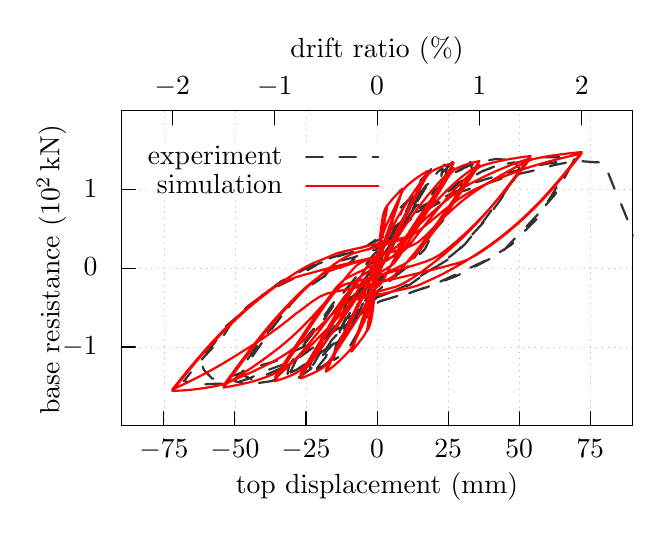
\begin{tikzpicture}[gnuplot]
%% generated with GNUPLOT 5.2p6 (Lua 5.3; terminal rev. Nov 2018, script rev. 107)
%% 07/24/2019 03:13:03
\path (0.000,0.000) rectangle (6.500,4.000);
\gpcolor{color=gp lt color axes}
\gpsetlinetype{gp lt axes}
\gpsetdashtype{gp dt axes}
\gpsetlinewidth{0.50}
\draw[gp path] (0.000,1.000)--(6.499,1.000);
\gpcolor{color=gp lt color border}
\gpsetlinetype{gp lt border}
\gpsetdashtype{gp dt solid}
\gpsetlinewidth{1.00}
\draw[gp path] (0.000,1.000)--(0.180,1.000);
\node[gp node right] at (-0.184,1.000) {$-1$};
\gpcolor{color=gp lt color axes}
\gpsetlinetype{gp lt axes}
\gpsetdashtype{gp dt axes}
\gpsetlinewidth{0.50}
\draw[gp path] (0.000,2.000)--(6.499,2.000);
\gpcolor{color=gp lt color border}
\gpsetlinetype{gp lt border}
\gpsetdashtype{gp dt solid}
\gpsetlinewidth{1.00}
\draw[gp path] (0.000,2.000)--(0.180,2.000);
\node[gp node right] at (-0.184,2.000) {$0$};
\gpcolor{color=gp lt color axes}
\gpsetlinetype{gp lt axes}
\gpsetdashtype{gp dt axes}
\gpsetlinewidth{0.50}
\draw[gp path] (0.000,2.999)--(0.325,2.999);
\draw[gp path] (3.449,2.999)--(6.499,2.999);
\gpcolor{color=gp lt color border}
\gpsetlinetype{gp lt border}
\gpsetdashtype{gp dt solid}
\gpsetlinewidth{1.00}
\draw[gp path] (0.000,2.999)--(0.180,2.999);
\node[gp node right] at (-0.184,2.999) {$1$};
\gpcolor{color=gp lt color axes}
\gpsetlinetype{gp lt axes}
\gpsetdashtype{gp dt axes}
\gpsetlinewidth{0.50}
\draw[gp path] (0.542,0.000)--(0.542,2.861);
\draw[gp path] (0.542,3.599)--(0.542,3.999);
\gpcolor{color=gp lt color border}
\gpsetlinetype{gp lt border}
\gpsetdashtype{gp dt solid}
\gpsetlinewidth{1.00}
\draw[gp path] (0.542,0.000)--(0.542,0.180);
\node[gp node center] at (0.542,-0.308) {$-75$};
\gpcolor{color=gp lt color axes}
\gpsetlinetype{gp lt axes}
\gpsetdashtype{gp dt axes}
\gpsetlinewidth{0.50}
\draw[gp path] (1.444,0.000)--(1.444,2.861);
\draw[gp path] (1.444,3.599)--(1.444,3.999);
\gpcolor{color=gp lt color border}
\gpsetlinetype{gp lt border}
\gpsetdashtype{gp dt solid}
\gpsetlinewidth{1.00}
\draw[gp path] (1.444,0.000)--(1.444,0.180);
\node[gp node center] at (1.444,-0.308) {$-50$};
\gpcolor{color=gp lt color axes}
\gpsetlinetype{gp lt axes}
\gpsetdashtype{gp dt axes}
\gpsetlinewidth{0.50}
\draw[gp path] (2.347,0.000)--(2.347,2.861);
\draw[gp path] (2.347,3.599)--(2.347,3.999);
\gpcolor{color=gp lt color border}
\gpsetlinetype{gp lt border}
\gpsetdashtype{gp dt solid}
\gpsetlinewidth{1.00}
\draw[gp path] (2.347,0.000)--(2.347,0.180);
\node[gp node center] at (2.347,-0.308) {$-25$};
\gpcolor{color=gp lt color axes}
\gpsetlinetype{gp lt axes}
\gpsetdashtype{gp dt axes}
\gpsetlinewidth{0.50}
\draw[gp path] (3.250,0.000)--(3.250,2.861);
\draw[gp path] (3.250,3.599)--(3.250,3.999);
\gpcolor{color=gp lt color border}
\gpsetlinetype{gp lt border}
\gpsetdashtype{gp dt solid}
\gpsetlinewidth{1.00}
\draw[gp path] (3.250,0.000)--(3.250,0.180);
\node[gp node center] at (3.250,-0.308) {$0$};
\gpcolor{color=gp lt color axes}
\gpsetlinetype{gp lt axes}
\gpsetdashtype{gp dt axes}
\gpsetlinewidth{0.50}
\draw[gp path] (4.152,0.000)--(4.152,3.999);
\gpcolor{color=gp lt color border}
\gpsetlinetype{gp lt border}
\gpsetdashtype{gp dt solid}
\gpsetlinewidth{1.00}
\draw[gp path] (4.152,0.000)--(4.152,0.180);
\node[gp node center] at (4.152,-0.308) {$25$};
\gpcolor{color=gp lt color axes}
\gpsetlinetype{gp lt axes}
\gpsetdashtype{gp dt axes}
\gpsetlinewidth{0.50}
\draw[gp path] (5.055,0.000)--(5.055,3.999);
\gpcolor{color=gp lt color border}
\gpsetlinetype{gp lt border}
\gpsetdashtype{gp dt solid}
\gpsetlinewidth{1.00}
\draw[gp path] (5.055,0.000)--(5.055,0.180);
\node[gp node center] at (5.055,-0.308) {$50$};
\gpcolor{color=gp lt color axes}
\gpsetlinetype{gp lt axes}
\gpsetdashtype{gp dt axes}
\gpsetlinewidth{0.50}
\draw[gp path] (5.957,0.000)--(5.957,3.999);
\gpcolor{color=gp lt color border}
\gpsetlinetype{gp lt border}
\gpsetdashtype{gp dt solid}
\gpsetlinewidth{1.00}
\draw[gp path] (5.957,0.000)--(5.957,0.180);
\node[gp node center] at (5.957,-0.308) {$75$};
\draw[gp path] (0.650,3.999)--(0.650,3.819);
\node[gp node center] at (0.650,4.307) {$-2$};
\draw[gp path] (1.950,3.999)--(1.950,3.819);
\node[gp node center] at (1.950,4.307) {$-1$};
\draw[gp path] (3.250,3.999)--(3.250,3.819);
\node[gp node center] at (3.250,4.307) {$0$};
\draw[gp path] (4.549,3.999)--(4.549,3.819);
\node[gp node center] at (4.549,4.307) {$1$};
\draw[gp path] (5.849,3.999)--(5.849,3.819);
\node[gp node center] at (5.849,4.307) {$2$};
\draw[gp path] (0.000,3.999)--(0.000,0.000)--(6.499,0.000)--(6.499,3.999)--cycle;
\node[gp node center,rotate=-270] at (-0.860,1.999) {base resistance (\SI{E2}{\kilo\newton})};
\node[gp node center] at (3.249,-0.769) {top displacement (\si{\milli\metre})};
\node[gp node center] at (3.249,4.769) {drift ratio (\si{\percent})};
\node[gp node right] at (2.165,3.414) {experiment};
\gpcolor{rgb color={0.200,0.200,0.200}}
\gpsetdashtype{gp dt 2}
\gpsetlinewidth{2.00}
\draw[gp path] (2.349,3.414)--(3.265,3.414);
\draw[gp path] (3.272,1.983)--(3.332,2.200)--(3.362,2.405)--(3.452,2.600)--(3.527,2.751)%
  --(3.662,2.881)--(3.737,3.032)--(3.812,3.108)--(3.767,2.924)--(3.692,2.729)--(3.587,2.546)%
  --(3.497,2.383)--(3.437,2.254)--(3.302,2.016)--(3.182,1.745)--(3.122,1.508)--(3.122,1.345)%
  --(3.017,1.205)--(2.942,1.075)--(2.897,1.000)--(2.777,0.881)--(2.702,0.837)--(2.717,1.000)%
  --(2.792,1.248)--(2.912,1.486)--(3.017,1.702)--(3.107,1.864)--(3.242,2.070)--(3.377,2.319)%
  --(3.512,2.589)--(3.587,2.794)--(3.692,2.935)--(3.827,3.075)--(3.857,3.151)--(3.737,2.827)%
  --(3.662,2.654)--(3.557,2.470)--(3.437,2.275)--(3.302,2.005)--(3.152,1.756)--(3.077,1.518)%
  --(2.972,1.345)--(2.882,1.194)--(2.792,1.086)--(2.717,0.956)--(2.747,1.172)--(2.912,1.443)%
  --(3.047,1.691)--(3.137,1.918)--(3.242,2.113)--(3.452,2.427)--(3.632,2.751)--(3.722,2.967)%
  --(3.812,3.129)--(3.917,3.227)--(3.962,3.313)--(4.007,3.346)--(4.142,3.302)--(4.112,3.140)%
  --(4.007,2.967)--(3.947,2.837)--(3.842,2.686)--(3.752,2.567)--(3.662,2.427)--(3.557,2.232)%
  --(3.467,2.102)--(3.362,1.929)--(3.212,1.724)--(3.062,1.540)--(2.987,1.356)--(2.807,1.107)%
  --(2.732,0.935)--(2.657,0.826)--(2.567,0.762)--(2.462,0.697)--(2.372,0.653)--(2.417,0.826)%
  --(2.552,1.010)--(2.657,1.172)--(2.792,1.399)--(2.867,1.562)--(3.002,1.756)--(3.182,1.972)%
  --(3.392,2.264)--(3.662,2.686)--(3.812,2.935)--(3.872,3.032)--(3.947,3.118)--(4.022,3.227)%
  --(4.082,3.270)--(4.052,3.075)--(3.932,2.805)--(3.767,2.610)--(3.647,2.437)--(3.557,2.221)%
  --(3.437,2.016)--(3.212,1.799)--(3.002,1.540)--(2.897,1.280)--(2.747,1.053)--(2.657,1.010)%
  --(2.597,0.870)--(2.492,0.740)--(2.387,0.686)--(2.537,0.945)--(2.627,1.183)--(2.762,1.432)%
  --(3.002,1.713)--(3.152,1.951)--(3.332,2.264)--(3.527,2.546)--(3.692,2.816)--(3.872,3.054)%
  --(4.022,3.162)--(4.157,3.291)--(4.202,3.346)--(4.307,3.346)--(4.442,3.346)--(4.457,3.227)%
  --(4.367,3.064)--(4.292,2.946)--(4.187,2.805)--(4.082,2.600)--(3.947,2.448)--(3.827,2.275)%
  --(3.722,2.135)--(3.617,2.070)--(3.542,1.983)--(3.467,1.897)--(3.332,1.756)--(3.137,1.562)%
  --(2.972,1.389)--(2.822,1.205)--(2.717,1.064)--(2.597,0.935)--(2.402,0.718)--(2.297,0.643)%
  --(2.237,0.599)--(2.102,0.599)--(2.132,0.762)--(2.252,0.945)--(2.417,1.151)--(2.597,1.378)%
  --(2.762,1.626)--(2.942,1.821)--(3.122,2.016)--(3.287,2.167)--(3.587,2.567)--(3.737,2.783)%
  --(3.887,2.892)--(4.037,3.010)--(4.052,3.032)--(4.172,3.173)--(4.292,3.248)--(4.397,3.313)%
  --(4.352,3.151)--(4.292,2.967)--(4.142,2.762)--(3.992,2.524)--(3.857,2.243)--(3.632,2.016)%
  --(3.452,1.875)--(3.257,1.713)--(3.122,1.551)--(3.002,1.453)--(2.852,1.280)--(2.672,1.086)%
  --(2.597,0.967)--(2.432,0.848)--(2.342,0.783)--(2.222,0.697)--(2.132,0.643)--(2.252,0.902)%
  --(2.357,1.129)--(2.537,1.334)--(2.687,1.551)--(2.882,1.767)--(3.017,1.929)--(3.182,2.145)%
  --(3.437,2.416)--(3.572,2.675)--(3.722,2.848)--(3.992,2.999)--(4.217,3.194)--(4.382,3.291)%
  --(4.547,3.346)--(4.757,3.389)--(4.907,3.378)--(4.967,3.324)--(5.072,3.259)--(4.997,3.140)%
  --(4.907,3.010)--(4.817,2.870)--(4.697,2.708)--(4.607,2.589)--(4.427,2.394)--(4.292,2.243)%
  --(4.172,2.145)--(4.007,2.027)--(3.722,1.854)--(3.587,1.767)--(3.407,1.691)--(3.287,1.670)%
  --(3.212,1.594)--(2.987,1.389)--(2.762,1.205)--(2.672,1.032)--(2.417,0.837)--(2.237,0.718)%
  --(2.042,0.621)--(1.907,0.567)--(1.682,0.534)--(1.562,0.534)--(1.442,0.567)--(1.532,0.740)%
  --(1.697,0.978)--(1.832,1.151)--(2.042,1.389)--(2.222,1.637)--(2.417,1.789)--(2.627,1.929)%
  --(2.867,2.048)--(3.077,2.200)--(3.347,2.362)--(3.692,2.719)--(4.037,2.902)--(4.262,3.043)%
  --(4.592,3.237)--(4.817,3.313)--(4.997,3.346)--(5.072,3.248)--(4.922,3.043)--(4.832,2.902)%
  --(4.697,2.729)--(4.547,2.524)--(4.367,2.308)--(4.187,2.135)--(3.962,1.994)--(3.812,1.897)%
  --(3.662,1.789)--(3.467,1.713)--(3.212,1.616)--(3.002,1.453)--(2.777,1.280)--(2.567,1.097)%
  --(2.387,0.978)--(2.207,0.837)--(2.027,0.729)--(1.832,0.643)--(1.682,0.578)--(1.622,0.610)%
  --(1.516,0.653)--(1.651,0.859)--(1.802,1.075)--(1.982,1.324)--(2.162,1.551)--(2.357,1.767)%
  --(2.582,1.897)--(2.672,2.016)--(2.807,2.102)--(2.942,2.135)--(3.242,2.243)--(3.542,2.513)%
  --(3.722,2.708)--(4.022,2.848)--(4.277,3.086)--(4.577,3.227)--(4.787,3.313)--(4.983,3.335)%
  --(5.162,3.367)--(5.327,3.410)--(5.583,3.410)--(5.762,3.400)--(5.718,3.313)--(5.567,3.097)%
  --(5.448,2.892)--(5.343,2.740)--(5.192,2.578)--(5.013,2.394)--(4.832,2.200)--(4.607,2.081)%
  --(4.247,1.897)--(3.842,1.745)--(3.542,1.659)--(3.197,1.551)--(2.882,1.324)--(2.612,1.140)%
  --(2.447,1.000)--(2.252,0.859)--(2.102,0.794)--(1.832,0.697)--(1.622,0.599)--(1.412,0.534)%
  --(1.202,0.534)--(1.021,0.524)--(0.796,0.567)--(0.916,0.718)--(1.067,0.891)--(1.291,1.129)%
  --(1.412,1.324)--(1.607,1.518)--(1.787,1.648)--(2.027,1.832)--(2.342,1.994)--(2.537,2.091)%
  --(2.807,2.178)--(3.122,2.286)--(3.557,2.589)--(3.872,2.783)--(4.187,2.946)--(4.517,3.097)%
  --(4.877,3.205)--(5.267,3.302)--(5.567,3.356)--(5.732,3.335)--(5.643,3.173)--(5.508,2.935)%
  --(5.357,2.762)--(5.283,2.632)--(5.132,2.481)--(4.952,2.297)--(4.682,2.124)--(4.382,1.983)%
  --(4.007,1.810)--(3.677,1.691)--(3.287,1.583)--(3.062,1.432)--(2.777,1.248)--(2.447,1.064)%
  --(2.192,0.945)--(1.982,0.826)--(1.787,0.772)--(1.592,0.697)--(1.442,0.643)--(1.307,0.610)%
  --(1.156,0.599)--(1.051,0.708)--(1.021,0.794)--(1.007,0.870)--(1.186,1.053)--(1.337,1.270)%
  --(1.622,1.508)--(1.847,1.702)--(2.177,1.864)--(2.507,2.059)--(2.702,2.135)--(2.942,2.210)%
  --(3.272,2.362)--(3.572,2.556)--(3.947,2.783)--(4.262,2.956)--(4.607,3.064)--(4.937,3.173)%
  --(5.222,3.237)--(5.508,3.313)--(5.778,3.367)--(6.018,3.346)--(6.123,3.346)--(6.183,3.216)%
  --(6.243,3.064)--(6.318,2.892)--(6.393,2.708)--(6.468,2.524)--(6.499,2.419);
\gpcolor{color=gp lt color border}
\node[gp node right] at (2.165,3.045) {simulation};
\gpcolor{rgb color={1.000,0.000,0.000}}
\gpsetdashtype{gp dt solid}
\draw[gp path] (2.349,3.045)--(3.265,3.045);
\draw[gp path] (3.250,2.000)--(3.255,2.054)--(3.260,2.108)--(3.265,2.163)--(3.270,2.217)%
  --(3.275,2.271)--(3.281,2.324)--(3.286,2.377)--(3.291,2.427)--(3.296,2.474)--(3.301,2.518)%
  --(3.307,2.557)--(3.312,2.593)--(3.317,2.624)--(3.322,2.652)--(3.327,2.676)--(3.333,2.697)%
  --(3.338,2.714)--(3.343,2.729)--(3.348,2.742)--(3.353,2.754)--(3.359,2.765)--(3.364,2.774)%
  --(3.369,2.783)--(3.374,2.792)--(3.379,2.800)--(3.374,2.767)--(3.369,2.735)--(3.364,2.703)%
  --(3.359,2.671)--(3.353,2.638)--(3.348,2.606)--(3.343,2.577)--(3.338,2.549)--(3.333,2.524)%
  --(3.327,2.502)--(3.322,2.480)--(3.317,2.457)--(3.312,2.435)--(3.307,2.412)--(3.301,2.388)%
  --(3.296,2.365)--(3.291,2.338)--(3.286,2.306)--(3.281,2.270)--(3.275,2.229)--(3.270,2.180)%
  --(3.265,2.130)--(3.260,2.081)--(3.255,2.031)--(3.250,1.982)--(3.244,1.930)--(3.239,1.876)%
  --(3.234,1.823)--(3.229,1.769)--(3.224,1.720)--(3.218,1.673)--(3.213,1.621)--(3.208,1.572)%
  --(3.203,1.525)--(3.198,1.483)--(3.192,1.443)--(3.187,1.408)--(3.182,1.377)--(3.177,1.349)%
  --(3.172,1.325)--(3.166,1.304)--(3.161,1.287)--(3.156,1.272)--(3.151,1.258)--(3.146,1.246)%
  --(3.140,1.236)--(3.135,1.226)--(3.130,1.216)--(3.125,1.208)--(3.120,1.200)--(3.125,1.232)%
  --(3.130,1.264)--(3.135,1.297)--(3.140,1.329)--(3.146,1.361)--(3.151,1.393)--(3.156,1.422)%
  --(3.161,1.450)--(3.166,1.475)--(3.172,1.498)--(3.177,1.520)--(3.182,1.543)--(3.187,1.566)%
  --(3.192,1.589)--(3.198,1.613)--(3.203,1.636)--(3.208,1.661)--(3.213,1.693)--(3.218,1.729)%
  --(3.224,1.768)--(3.229,1.817)--(3.234,1.866)--(3.239,1.916)--(3.244,1.965)--(3.249,2.011)%
  --(3.255,2.058)--(3.260,2.107)--(3.265,2.156)--(3.270,2.205)--(3.275,2.250)--(3.281,2.286)%
  --(3.286,2.321)--(3.291,2.353)--(3.296,2.379)--(3.301,2.403)--(3.307,2.426)--(3.312,2.450)%
  --(3.317,2.474)--(3.322,2.497)--(3.327,2.520)--(3.333,2.542)--(3.338,2.564)--(3.343,2.587)%
  --(3.348,2.613)--(3.353,2.641)--(3.359,2.672)--(3.364,2.703)--(3.369,2.735)--(3.374,2.766)%
  --(3.379,2.797)--(3.374,2.765)--(3.369,2.733)--(3.364,2.701)--(3.359,2.669)--(3.353,2.637)%
  --(3.348,2.609)--(3.343,2.583)--(3.338,2.559)--(3.333,2.537)--(3.327,2.514)--(3.322,2.491)%
  --(3.317,2.467)--(3.312,2.444)--(3.307,2.420)--(3.301,2.395)--(3.296,2.371)--(3.291,2.344)%
  --(3.286,2.312)--(3.281,2.276)--(3.275,2.240)--(3.270,2.194)--(3.265,2.145)--(3.260,2.095)%
  --(3.255,2.046)--(3.250,1.999)--(3.244,1.952)--(3.239,1.903)--(3.234,1.853)--(3.229,1.804)%
  --(3.224,1.758)--(3.218,1.722)--(3.213,1.686)--(3.208,1.654)--(3.203,1.627)--(3.198,1.603)%
  --(3.192,1.579)--(3.187,1.555)--(3.182,1.531)--(3.177,1.507)--(3.172,1.484)--(3.166,1.461)%
  --(3.161,1.439)--(3.156,1.416)--(3.151,1.389)--(3.146,1.360)--(3.140,1.329)--(3.135,1.297)%
  --(3.130,1.264)--(3.125,1.232)--(3.120,1.200)--(3.125,1.232)--(3.130,1.264)--(3.135,1.297)%
  --(3.140,1.329)--(3.146,1.361)--(3.151,1.392)--(3.156,1.422)--(3.161,1.452)--(3.166,1.480)%
  --(3.172,1.508)--(3.177,1.536)--(3.182,1.563)--(3.187,1.590)--(3.192,1.618)--(3.198,1.646)%
  --(3.203,1.675)--(3.208,1.703)--(3.213,1.734)--(3.218,1.767)--(3.224,1.799)--(3.229,1.832)%
  --(3.234,1.873)--(3.239,1.916)--(3.244,1.959)--(3.249,2.000)--(3.262,2.120)--(3.275,2.240)%
  --(3.288,2.328)--(3.301,2.396)--(3.314,2.456)--(3.327,2.514)--(3.340,2.571)--(3.353,2.637)%
  --(3.366,2.717)--(3.379,2.797)--(3.392,2.815)--(3.405,2.830)--(3.418,2.845)--(3.431,2.862)%
  --(3.444,2.878)--(3.457,2.893)--(3.470,2.905)--(3.483,2.918)--(3.496,2.932)--(3.509,2.947)%
  --(3.522,2.962)--(3.535,2.976)--(3.548,2.988)--(3.561,3.000)--(3.574,3.012)--(3.561,2.972)%
  --(3.548,2.933)--(3.535,2.893)--(3.522,2.854)--(3.509,2.817)--(3.496,2.779)--(3.483,2.741)%
  --(3.470,2.704)--(3.457,2.668)--(3.444,2.631)--(3.431,2.594)--(3.418,2.558)--(3.405,2.521)%
  --(3.392,2.485)--(3.379,2.448)--(3.366,2.411)--(3.353,2.375)--(3.340,2.338)--(3.327,2.297)%
  --(3.314,2.255)--(3.301,2.210)--(3.288,2.158)--(3.275,2.106)--(3.262,2.047)--(3.250,1.963)%
  --(3.237,1.836)--(3.224,1.735)--(3.211,1.649)--(3.198,1.587)--(3.185,1.531)--(3.172,1.476)%
  --(3.159,1.419)--(3.146,1.357)--(3.133,1.279)--(3.120,1.209)--(3.107,1.185)--(3.094,1.161)%
  --(3.081,1.141)--(3.068,1.120)--(3.055,1.104)--(3.042,1.089)--(3.029,1.072)--(3.016,1.054)%
  --(3.003,1.037)--(2.990,1.020)--(2.977,1.003)--(2.964,0.987)--(2.951,0.972)--(2.938,0.957)%
  --(2.925,0.942)--(2.938,0.979)--(2.951,1.017)--(2.964,1.056)--(2.977,1.095)--(2.990,1.133)%
  --(3.003,1.171)--(3.016,1.209)--(3.029,1.246)--(3.042,1.284)--(3.055,1.322)--(3.068,1.361)%
  --(3.081,1.399)--(3.094,1.438)--(3.107,1.482)--(3.120,1.529)--(3.133,1.578)--(3.146,1.628)%
  --(3.159,1.678)--(3.172,1.728)--(3.185,1.778)--(3.198,1.830)--(3.211,1.884)--(3.224,1.938)%
  --(3.237,1.994)--(3.249,2.074)--(3.262,2.161)--(3.275,2.228)--(3.288,2.305)--(3.301,2.359)%
  --(3.314,2.403)--(3.327,2.444)--(3.340,2.478)--(3.353,2.512)--(3.366,2.542)--(3.379,2.570)%
  --(3.392,2.598)--(3.405,2.626)--(3.418,2.653)--(3.431,2.681)--(3.444,2.709)--(3.457,2.736)%
  --(3.470,2.764)--(3.483,2.792)--(3.496,2.819)--(3.509,2.846)--(3.522,2.873)--(3.535,2.899)%
  --(3.548,2.928)--(3.561,2.964)--(3.574,2.998)--(3.561,2.960)--(3.548,2.922)--(3.535,2.881)%
  --(3.522,2.841)--(3.509,2.802)--(3.496,2.762)--(3.483,2.722)--(3.470,2.682)--(3.457,2.643)%
  --(3.444,2.603)--(3.431,2.563)--(3.418,2.523)--(3.405,2.484)--(3.392,2.444)--(3.379,2.404)%
  --(3.366,2.364)--(3.353,2.325)--(3.340,2.285)--(3.327,2.243)--(3.314,2.201)--(3.301,2.157)%
  --(3.288,2.111)--(3.275,2.070)--(3.262,2.039)--(3.250,1.996)--(3.237,1.953)--(3.224,1.921)%
  --(3.211,1.882)--(3.198,1.828)--(3.185,1.774)--(3.172,1.722)--(3.159,1.673)--(3.146,1.623)%
  --(3.133,1.573)--(3.120,1.525)--(3.107,1.480)--(3.094,1.438)--(3.081,1.400)--(3.068,1.361)%
  --(3.055,1.323)--(3.042,1.285)--(3.029,1.248)--(3.016,1.211)--(3.003,1.174)--(2.990,1.136)%
  --(2.977,1.099)--(2.964,1.061)--(2.951,1.022)--(2.938,0.985)--(2.925,0.951)--(2.938,0.989)%
  --(2.951,1.026)--(2.964,1.066)--(2.977,1.104)--(2.990,1.142)--(3.003,1.180)--(3.016,1.218)%
  --(3.029,1.255)--(3.042,1.293)--(3.055,1.331)--(3.068,1.370)--(3.081,1.408)--(3.094,1.447)%
  --(3.107,1.488)--(3.120,1.533)--(3.133,1.581)--(3.146,1.631)--(3.159,1.681)--(3.172,1.731)%
  --(3.185,1.780)--(3.198,1.833)--(3.211,1.887)--(3.224,1.925)--(3.237,1.957)--(3.249,1.999)%
  --(3.275,2.073)--(3.301,2.159)--(3.327,2.244)--(3.353,2.323)--(3.379,2.403)--(3.405,2.483)%
  --(3.431,2.562)--(3.457,2.642)--(3.483,2.721)--(3.509,2.800)--(3.535,2.878)--(3.561,2.957)%
  --(3.587,3.006)--(3.613,3.032)--(3.639,3.058)--(3.665,3.080)--(3.691,3.101)--(3.717,3.121)%
  --(3.743,3.140)--(3.769,3.159)--(3.795,3.176)--(3.821,3.193)--(3.847,3.208)--(3.873,3.224)%
  --(3.899,3.238)--(3.873,3.187)--(3.847,3.136)--(3.821,3.087)--(3.795,3.038)--(3.769,2.990)%
  --(3.743,2.941)--(3.717,2.892)--(3.691,2.844)--(3.665,2.795)--(3.639,2.745)--(3.613,2.695)%
  --(3.587,2.645)--(3.561,2.595)--(3.535,2.545)--(3.509,2.492)--(3.483,2.437)--(3.457,2.379)%
  --(3.431,2.318)--(3.405,2.258)--(3.379,2.198)--(3.353,2.137)--(3.327,2.077)--(3.301,2.014)%
  --(3.275,1.934)--(3.250,1.831)--(3.224,1.751)--(3.198,1.671)--(3.172,1.579)--(3.146,1.495)%
  --(3.120,1.415)--(3.094,1.343)--(3.068,1.284)--(3.042,1.228)--(3.016,1.174)--(2.990,1.121)%
  --(2.964,1.069)--(2.938,1.009)--(2.912,0.971)--(2.886,0.940)--(2.860,0.912)--(2.834,0.885)%
  --(2.808,0.859)--(2.782,0.834)--(2.756,0.810)--(2.730,0.787)--(2.704,0.764)--(2.678,0.743)%
  --(2.652,0.723)--(2.626,0.704)--(2.600,0.687)--(2.626,0.739)--(2.652,0.793)--(2.678,0.847)%
  --(2.704,0.900)--(2.730,0.954)--(2.756,1.008)--(2.782,1.061)--(2.808,1.114)--(2.834,1.168)%
  --(2.860,1.221)--(2.886,1.274)--(2.912,1.327)--(2.938,1.381)--(2.964,1.435)--(2.990,1.489)%
  --(3.016,1.543)--(3.042,1.599)--(3.068,1.655)--(3.094,1.713)--(3.120,1.776)--(3.146,1.852)%
  --(3.172,1.933)--(3.198,2.017)--(3.224,2.105)--(3.249,2.174)--(3.275,2.226)--(3.301,2.266)%
  --(3.327,2.297)--(3.353,2.337)--(3.379,2.388)--(3.405,2.440)--(3.431,2.492)--(3.457,2.545)%
  --(3.483,2.595)--(3.509,2.643)--(3.535,2.687)--(3.561,2.729)--(3.587,2.770)--(3.613,2.810)%
  --(3.639,2.851)--(3.665,2.891)--(3.691,2.930)--(3.717,2.969)--(3.743,3.007)--(3.769,3.044)%
  --(3.795,3.080)--(3.821,3.115)--(3.847,3.150)--(3.873,3.184)--(3.899,3.219)--(3.873,3.168)%
  --(3.847,3.115)--(3.821,3.064)--(3.795,3.013)--(3.769,2.962)--(3.743,2.911)--(3.717,2.859)%
  --(3.691,2.808)--(3.665,2.756)--(3.639,2.704)--(3.613,2.652)--(3.587,2.600)--(3.561,2.548)%
  --(3.535,2.495)--(3.509,2.442)--(3.483,2.386)--(3.457,2.327)--(3.431,2.266)--(3.405,2.203)%
  --(3.379,2.141)--(3.353,2.094)--(3.327,2.057)--(3.301,2.021)--(3.275,1.996)--(3.250,1.973)%
  --(3.224,1.949)--(3.198,1.915)--(3.172,1.867)--(3.146,1.816)--(3.120,1.752)--(3.094,1.690)%
  --(3.068,1.632)--(3.042,1.577)--(3.016,1.521)--(2.990,1.467)--(2.964,1.413)--(2.938,1.360)%
  --(2.912,1.307)--(2.886,1.254)--(2.860,1.201)--(2.834,1.149)--(2.808,1.097)--(2.782,1.046)%
  --(2.756,0.994)--(2.730,0.943)--(2.704,0.893)--(2.678,0.844)--(2.652,0.797)--(2.626,0.750)%
  --(2.600,0.711)--(2.626,0.762)--(2.652,0.816)--(2.678,0.869)--(2.704,0.922)--(2.730,0.976)%
  --(2.756,1.029)--(2.782,1.082)--(2.808,1.136)--(2.834,1.189)--(2.860,1.241)--(2.886,1.295)%
  --(2.912,1.347)--(2.938,1.401)--(2.964,1.455)--(2.990,1.509)--(3.016,1.563)--(3.042,1.618)%
  --(3.068,1.674)--(3.094,1.731)--(3.120,1.793)--(3.146,1.853)--(3.172,1.901)--(3.198,1.948)%
  --(3.224,1.974)--(3.249,1.998)--(3.288,2.033)--(3.327,2.074)--(3.366,2.130)--(3.405,2.215)%
  --(3.444,2.309)--(3.483,2.396)--(3.522,2.478)--(3.561,2.557)--(3.600,2.635)--(3.639,2.713)%
  --(3.678,2.790)--(3.717,2.866)--(3.756,2.941)--(3.795,3.014)--(3.834,3.086)--(3.873,3.158)%
  --(3.912,3.207)--(3.951,3.235)--(3.990,3.256)--(4.029,3.274)--(4.068,3.289)--(4.107,3.304)%
  --(4.146,3.316)--(4.185,3.328)--(4.224,3.339)--(4.185,3.274)--(4.146,3.209)--(4.107,3.145)%
  --(4.068,3.081)--(4.029,3.017)--(3.990,2.954)--(3.951,2.890)--(3.912,2.826)--(3.873,2.762)%
  --(3.834,2.699)--(3.795,2.635)--(3.756,2.572)--(3.717,2.509)--(3.678,2.446)--(3.639,2.384)%
  --(3.600,2.322)--(3.561,2.261)--(3.522,2.200)--(3.483,2.138)--(3.444,2.069)--(3.405,1.997)%
  --(3.366,1.921)--(3.327,1.846)--(3.288,1.793)--(3.250,1.761)--(3.211,1.732)--(3.172,1.675)%
  --(3.133,1.607)--(3.094,1.523)--(3.055,1.453)--(3.016,1.388)--(2.977,1.324)--(2.938,1.263)%
  --(2.899,1.203)--(2.860,1.142)--(2.821,1.082)--(2.782,1.023)--(2.743,0.964)--(2.704,0.907)%
  --(2.665,0.853)--(2.626,0.801)--(2.587,0.759)--(2.548,0.729)--(2.509,0.705)--(2.470,0.684)%
  --(2.431,0.665)--(2.392,0.648)--(2.353,0.631)--(2.314,0.615)--(2.275,0.602)--(2.314,0.668)%
  --(2.353,0.735)--(2.392,0.801)--(2.431,0.868)--(2.470,0.934)--(2.509,1.000)--(2.548,1.067)%
  --(2.587,1.134)--(2.626,1.201)--(2.665,1.268)--(2.704,1.335)--(2.743,1.401)--(2.782,1.467)%
  --(2.821,1.533)--(2.860,1.598)--(2.899,1.662)--(2.938,1.726)--(2.977,1.789)--(3.016,1.851)%
  --(3.055,1.914)--(3.094,1.977)--(3.133,2.035)--(3.172,2.087)--(3.211,2.110)--(3.249,2.132)%
  --(3.288,2.154)--(3.327,2.176)--(3.366,2.198)--(3.405,2.237)--(3.444,2.291)--(3.483,2.351)%
  --(3.522,2.413)--(3.561,2.473)--(3.600,2.530)--(3.639,2.587)--(3.678,2.642)--(3.717,2.696)%
  --(3.756,2.749)--(3.795,2.801)--(3.834,2.851)--(3.873,2.900)--(3.912,2.948)--(3.951,2.994)%
  --(3.990,3.040)--(4.029,3.083)--(4.068,3.126)--(4.107,3.166)--(4.146,3.206)--(4.185,3.244)%
  --(4.224,3.278)--(4.185,3.213)--(4.146,3.148)--(4.107,3.084)--(4.068,3.020)--(4.029,2.955)%
  --(3.990,2.891)--(3.951,2.827)--(3.912,2.763)--(3.873,2.699)--(3.834,2.635)--(3.795,2.571)%
  --(3.756,2.508)--(3.717,2.445)--(3.678,2.382)--(3.639,2.320)--(3.600,2.258)--(3.561,2.197)%
  --(3.522,2.137)--(3.483,2.087)--(3.444,2.044)--(3.405,2.018)--(3.366,1.993)--(3.327,1.969)%
  --(3.288,1.945)--(3.250,1.921)--(3.211,1.898)--(3.172,1.875)--(3.133,1.852)--(3.094,1.829)%
  --(3.055,1.792)--(3.016,1.739)--(2.977,1.675)--(2.938,1.609)--(2.899,1.543)--(2.860,1.478)%
  --(2.821,1.414)--(2.782,1.351)--(2.743,1.288)--(2.704,1.227)--(2.665,1.167)--(2.626,1.107)%
  --(2.587,1.050)--(2.548,0.994)--(2.509,0.940)--(2.470,0.887)--(2.431,0.835)--(2.392,0.785)%
  --(2.353,0.735)--(2.314,0.687)--(2.275,0.647)--(2.314,0.713)--(2.353,0.780)--(2.392,0.846)%
  --(2.431,0.913)--(2.470,0.979)--(2.509,1.044)--(2.548,1.111)--(2.587,1.178)--(2.626,1.245)%
  --(2.665,1.311)--(2.704,1.378)--(2.743,1.444)--(2.782,1.510)--(2.821,1.575)--(2.860,1.640)%
  --(2.899,1.704)--(2.938,1.767)--(2.977,1.829)--(3.016,1.874)--(3.055,1.906)--(3.094,1.930)%
  --(3.133,1.955)--(3.172,1.979)--(3.211,2.003)--(3.250,2.026)--(3.301,2.057)--(3.353,2.089)%
  --(3.405,2.121)--(3.457,2.158)--(3.509,2.222)--(3.561,2.305)--(3.613,2.389)--(3.665,2.472)%
  --(3.717,2.553)--(3.769,2.632)--(3.821,2.709)--(3.873,2.785)--(3.925,2.859)--(3.977,2.932)%
  --(4.029,3.003)--(4.081,3.072)--(4.133,3.139)--(4.185,3.205)--(4.237,3.256)--(4.289,3.282)%
  --(4.341,3.305)--(4.393,3.322)--(4.445,3.337)--(4.497,3.350)--(4.549,3.362)--(4.497,3.283)%
  --(4.445,3.205)--(4.393,3.127)--(4.341,3.050)--(4.289,2.973)--(4.237,2.896)--(4.185,2.820)%
  --(4.133,2.744)--(4.081,2.670)--(4.029,2.597)--(3.977,2.524)--(3.925,2.453)--(3.873,2.383)%
  --(3.821,2.315)--(3.769,2.248)--(3.717,2.183)--(3.665,2.120)--(3.613,2.059)--(3.561,1.999)%
  --(3.509,1.949)--(3.457,1.899)--(3.405,1.867)--(3.353,1.844)--(3.301,1.821)--(3.249,1.799)%
  --(3.198,1.776)--(3.146,1.755)--(3.094,1.735)--(3.042,1.689)--(2.990,1.622)--(2.938,1.543)%
  --(2.886,1.467)--(2.834,1.392)--(2.782,1.319)--(2.730,1.248)--(2.678,1.178)--(2.626,1.110)%
  --(2.574,1.044)--(2.522,0.980)--(2.470,0.918)--(2.418,0.857)--(2.366,0.799)--(2.314,0.743)%
  --(2.262,0.696)--(2.210,0.665)--(2.158,0.639)--(2.106,0.618)--(2.054,0.599)--(2.002,0.581)%
  --(1.950,0.567)--(2.002,0.647)--(2.054,0.728)--(2.106,0.808)--(2.158,0.887)--(2.210,0.966)%
  --(2.262,1.046)--(2.314,1.125)--(2.366,1.204)--(2.418,1.282)--(2.470,1.359)--(2.522,1.435)%
  --(2.574,1.510)--(2.626,1.583)--(2.678,1.654)--(2.730,1.723)--(2.782,1.791)--(2.834,1.858)%
  --(2.886,1.923)--(2.938,1.983)--(2.990,2.035)--(3.042,2.072)--(3.094,2.094)--(3.146,2.116)%
  --(3.198,2.137)--(3.250,2.158)--(3.301,2.180)--(3.353,2.202)--(3.405,2.223)--(3.457,2.244)%
  --(3.509,2.282)--(3.561,2.336)--(3.613,2.400)--(3.665,2.464)--(3.717,2.527)--(3.769,2.588)%
  --(3.821,2.649)--(3.873,2.708)--(3.925,2.766)--(3.977,2.823)--(4.029,2.879)--(4.081,2.933)%
  --(4.133,2.986)--(4.185,3.037)--(4.237,3.085)--(4.289,3.131)--(4.341,3.173)--(4.393,3.213)%
  --(4.445,3.250)--(4.497,3.285)--(4.549,3.317)--(4.497,3.239)--(4.445,3.161)--(4.393,3.083)%
  --(4.341,3.005)--(4.289,2.928)--(4.237,2.851)--(4.185,2.775)--(4.133,2.700)--(4.081,2.626)%
  --(4.029,2.552)--(3.977,2.480)--(3.925,2.409)--(3.873,2.340)--(3.821,2.272)--(3.769,2.206)%
  --(3.717,2.145)--(3.665,2.102)--(3.613,2.062)--(3.561,2.036)--(3.509,2.010)--(3.457,1.985)%
  --(3.405,1.961)--(3.353,1.936)--(3.301,1.913)--(3.249,1.889)--(3.198,1.866)--(3.146,1.843)%
  --(3.094,1.821)--(3.042,1.800)--(2.990,1.778)--(2.938,1.749)--(2.886,1.700)--(2.834,1.637)%
  --(2.782,1.564)--(2.730,1.492)--(2.678,1.421)--(2.626,1.351)--(2.574,1.283)--(2.522,1.215)%
  --(2.470,1.149)--(2.418,1.084)--(2.366,1.020)--(2.314,0.958)--(2.262,0.900)--(2.210,0.843)%
  --(2.158,0.790)--(2.106,0.739)--(2.054,0.690)--(2.002,0.643)--(1.950,0.609)--(2.002,0.689)%
  --(2.054,0.768)--(2.106,0.848)--(2.158,0.927)--(2.210,1.006)--(2.262,1.085)--(2.314,1.164)%
  --(2.366,1.242)--(2.418,1.319)--(2.470,1.395)--(2.522,1.470)--(2.574,1.543)--(2.626,1.615)%
  --(2.678,1.686)--(2.730,1.755)--(2.782,1.809)--(2.834,1.856)--(2.886,1.887)--(2.938,1.913)%
  --(2.990,1.939)--(3.042,1.964)--(3.094,1.988)--(3.146,2.013)--(3.198,2.037)--(3.250,2.061)%
  --(3.327,2.095)--(3.405,2.129)--(3.483,2.162)--(3.561,2.199)--(3.639,2.270)--(3.717,2.368)%
  --(3.795,2.470)--(3.873,2.570)--(3.951,2.667)--(4.029,2.762)--(4.107,2.855)--(4.185,2.945)%
  --(4.263,3.031)--(4.341,3.110)--(4.419,3.184)--(4.497,3.252)--(4.575,3.301)--(4.653,3.325)%
  --(4.731,3.345)--(4.809,3.363)--(4.887,3.379)--(4.965,3.392)--(5.043,3.405)--(5.121,3.416)%
  --(5.199,3.426)--(5.121,3.321)--(5.043,3.217)--(4.965,3.114)--(4.887,3.012)--(4.809,2.913)%
  --(4.731,2.818)--(4.653,2.726)--(4.575,2.637)--(4.497,2.553)--(4.419,2.471)--(4.341,2.394)%
  --(4.263,2.320)--(4.185,2.250)--(4.107,2.183)--(4.029,2.119)--(3.951,2.058)--(3.873,1.999)%
  --(3.795,1.942)--(3.717,1.888)--(3.639,1.840)--(3.561,1.795)--(3.483,1.764)--(3.405,1.743)%
  --(3.327,1.721)--(3.249,1.700)--(3.172,1.680)--(3.094,1.660)--(3.016,1.640)--(2.938,1.578)%
  --(2.860,1.499)--(2.782,1.410)--(2.704,1.324)--(2.626,1.240)--(2.548,1.160)--(2.470,1.081)%
  --(2.392,1.004)--(2.314,0.930)--(2.236,0.862)--(2.158,0.800)--(2.080,0.743)--(2.002,0.695)%
  --(1.924,0.652)--(1.846,0.621)--(1.768,0.593)--(1.690,0.568)--(1.612,0.548)--(1.534,0.531)%
  --(1.456,0.514)--(1.378,0.499)--(1.300,0.485)--(1.378,0.593)--(1.456,0.700)--(1.534,0.806)%
  --(1.612,0.911)--(1.690,1.012)--(1.768,1.111)--(1.846,1.208)--(1.924,1.301)--(2.002,1.391)%
  --(2.080,1.477)--(2.158,1.560)--(2.236,1.639)--(2.314,1.715)--(2.392,1.788)--(2.470,1.857)%
  --(2.548,1.924)--(2.626,1.988)--(2.704,2.050)--(2.782,2.104)--(2.860,2.147)--(2.938,2.187)%
  --(3.016,2.209)--(3.094,2.230)--(3.172,2.252)--(3.250,2.275)--(3.327,2.297)--(3.405,2.319)%
  --(3.483,2.341)--(3.561,2.363)--(3.639,2.415)--(3.717,2.490)--(3.795,2.564)--(3.873,2.637)%
  --(3.951,2.709)--(4.029,2.778)--(4.107,2.845)--(4.185,2.908)--(4.263,2.966)--(4.341,3.019)%
  --(4.419,3.066)--(4.497,3.108)--(4.575,3.148)--(4.653,3.185)--(4.731,3.221)--(4.809,3.255)%
  --(4.887,3.287)--(4.965,3.317)--(5.043,3.345)--(5.121,3.371)--(5.199,3.398)--(5.121,3.297)%
  --(5.043,3.197)--(4.965,3.099)--(4.887,3.002)--(4.809,2.907)--(4.731,2.816)--(4.653,2.728)%
  --(4.575,2.644)--(4.497,2.565)--(4.419,2.488)--(4.341,2.415)--(4.263,2.346)--(4.185,2.280)%
  --(4.107,2.217)--(4.029,2.162)--(3.951,2.119)--(3.873,2.087)--(3.795,2.061)--(3.717,2.037)%
  --(3.639,2.014)--(3.561,1.991)--(3.483,1.968)--(3.405,1.946)--(3.327,1.924)--(3.249,1.903)%
  --(3.172,1.882)--(3.094,1.861)--(3.016,1.841)--(2.938,1.822)--(2.860,1.803)--(2.782,1.766)%
  --(2.704,1.685)--(2.626,1.604)--(2.548,1.519)--(2.470,1.433)--(2.392,1.349)--(2.314,1.268)%
  --(2.236,1.192)--(2.158,1.120)--(2.080,1.053)--(2.002,0.989)--(1.924,0.929)--(1.846,0.871)%
  --(1.768,0.815)--(1.690,0.760)--(1.612,0.707)--(1.534,0.656)--(1.456,0.606)--(1.378,0.557)%
  --(1.300,0.513)--(1.378,0.620)--(1.456,0.727)--(1.534,0.832)--(1.612,0.936)--(1.690,1.037)%
  --(1.768,1.135)--(1.846,1.230)--(1.924,1.322)--(2.002,1.410)--(2.080,1.495)--(2.158,1.577)%
  --(2.236,1.655)--(2.314,1.731)--(2.392,1.798)--(2.470,1.861)--(2.548,1.918)--(2.626,1.960)%
  --(2.704,1.987)--(2.782,2.012)--(2.860,2.037)--(2.938,2.062)--(3.016,2.085)--(3.094,2.109)%
  --(3.172,2.132)--(3.250,2.154)--(3.353,2.183)--(3.457,2.213)--(3.561,2.245)--(3.665,2.277)%
  --(3.769,2.329)--(3.873,2.419)--(3.977,2.526)--(4.081,2.630)--(4.185,2.729)--(4.289,2.821)%
  --(4.393,2.904)--(4.497,2.978)--(4.601,3.047)--(4.705,3.111)--(4.809,3.173)--(4.913,3.232)%
  --(5.017,3.288)--(5.121,3.342)--(5.225,3.385)--(5.329,3.407)--(5.433,3.426)--(5.537,3.440)%
  --(5.641,3.454)--(5.745,3.466)--(5.849,3.476)--(5.745,3.345)--(5.641,3.217)--(5.537,3.093)%
  --(5.433,2.974)--(5.329,2.860)--(5.225,2.754)--(5.121,2.654)--(5.017,2.560)--(4.913,2.472)%
  --(4.809,2.389)--(4.705,2.311)--(4.601,2.238)--(4.497,2.169)--(4.393,2.103)--(4.289,2.041)%
  --(4.185,1.982)--(4.081,1.926)--(3.977,1.876)--(3.873,1.829)--(3.769,1.782)--(3.665,1.753)%
  --(3.561,1.730)--(3.457,1.707)--(3.353,1.684)--(3.249,1.662)--(3.146,1.640)--(3.042,1.619)%
  --(2.938,1.598)--(2.834,1.549)--(2.730,1.466)--(2.626,1.363)--(2.522,1.261)--(2.418,1.167)%
  --(2.314,1.080)--(2.210,0.997)--(2.106,0.922)--(2.002,0.857)--(1.898,0.799)--(1.794,0.747)%
  --(1.690,0.697)--(1.586,0.649)--(1.482,0.603)--(1.378,0.559)--(1.274,0.522)--(1.170,0.498)%
  --(1.066,0.480)--(0.962,0.466)--(0.858,0.455)--(0.754,0.447)--(0.650,0.444)--(0.754,0.573)%
  --(0.858,0.701)--(0.962,0.826)--(1.066,0.946)--(1.170,1.061)--(1.274,1.171)--(1.378,1.276)%
  --(1.482,1.375)--(1.586,1.469)--(1.690,1.558)--(1.794,1.642)--(1.898,1.722)--(2.002,1.798)%
  --(2.106,1.870)--(2.210,1.938)--(2.314,2.001)--(2.418,2.056)--(2.522,2.099)--(2.626,2.142)%
  --(2.730,2.186)--(2.834,2.216)--(2.938,2.239)--(3.042,2.262)--(3.146,2.287)--(3.250,2.311)%
  --(3.353,2.335)--(3.457,2.358)--(3.561,2.381)--(3.665,2.406)--(3.769,2.469)--(3.873,2.551)%
  --(3.977,2.635)--(4.081,2.722)--(4.185,2.804)--(4.289,2.881)--(4.393,2.948)--(4.497,3.005)%
  --(4.601,3.054)--(4.705,3.100)--(4.809,3.144)--(4.913,3.186)--(5.017,3.226)--(5.121,3.263)%
  --(5.225,3.297)--(5.329,3.328)--(5.433,3.357)--(5.537,3.384)--(5.641,3.410)--(5.745,3.435)%
  --(5.849,3.461)--(5.745,3.331)--(5.641,3.203)--(5.537,3.079)--(5.433,2.960)--(5.329,2.847)%
  --(5.225,2.742)--(5.121,2.643)--(5.017,2.549)--(4.913,2.461)--(4.809,2.378)--(4.705,2.301)%
  --(4.601,2.228)--(4.497,2.162)--(4.393,2.107)--(4.289,2.070)--(4.185,2.042)--(4.081,2.014)%
  --(3.977,1.988)--(3.873,1.962)--(3.769,1.936)--(3.665,1.912)--(3.561,1.887)--(3.457,1.863)%
  --(3.353,1.839)--(3.249,1.815)--(3.146,1.792)--(3.042,1.769)--(2.938,1.747)--(2.834,1.726)%
  --(2.730,1.704)--(2.626,1.684)--(2.522,1.640)--(2.418,1.572)--(2.314,1.493)--(2.210,1.417)%
  --(2.106,1.332)--(2.002,1.252)--(1.898,1.177)--(1.794,1.106)--(1.690,1.038)--(1.586,0.972)%
  --(1.482,0.907)--(1.378,0.843)--(1.274,0.780)--(1.170,0.721)--(1.066,0.664)--(0.962,0.610)%
  --(0.858,0.558)--(0.754,0.508)--(0.650,0.462)--(0.754,0.591)--(0.858,0.719)--(0.962,0.843)%
  --(1.066,0.963)--(1.170,1.078)--(1.274,1.187)--(1.378,1.291)--(1.482,1.390)--(1.586,1.484)%
  --(1.690,1.574)--(1.794,1.659)--(1.898,1.734)--(2.002,1.790)--(2.106,1.844)--(2.210,1.884)%
  --(2.314,1.914)--(2.418,1.943)--(2.522,1.971)--(2.626,1.999)--(2.730,2.025)--(2.834,2.051)%
  --(2.938,2.076)--(3.042,2.101)--(3.146,2.125)--(3.250,2.149);
\gpcolor{color=gp lt color border}
\gpsetlinewidth{1.00}
\draw[gp path] (0.000,3.999)--(0.000,0.000)--(6.499,0.000)--(6.499,3.999)--cycle;
%% coordinates of the plot area
\gpdefrectangularnode{gp plot 1}{\pgfpoint{0.000cm}{0.000cm}}{\pgfpoint{6.499cm}{3.999cm}}
\end{tikzpicture}
%% gnuplot variables

\caption{RW1 specimen}\label{fig:rw1_pushover}
\end{subfigure}\quad
\begin{subfigure}[b]{0.48\textwidth}
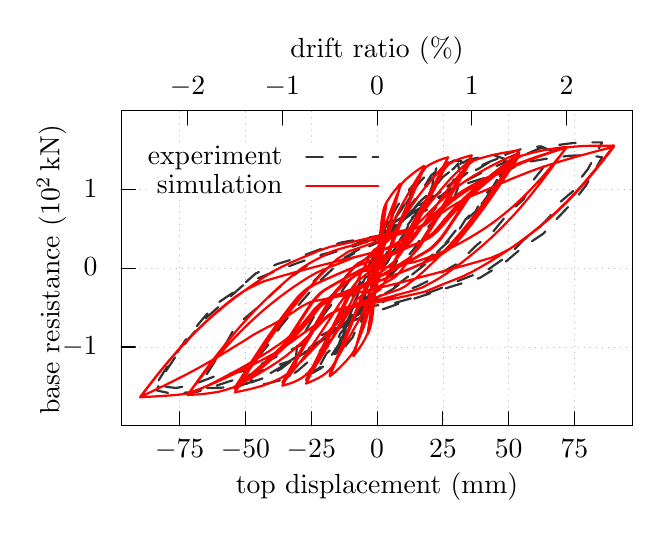
\begin{tikzpicture}[gnuplot]
%% generated with GNUPLOT 5.2p6 (Lua 5.3; terminal rev. Nov 2018, script rev. 107)
%% 07/24/2019 03:18:40
\path (0.000,0.000) rectangle (6.500,4.000);
\gpcolor{color=gp lt color axes}
\gpsetlinetype{gp lt axes}
\gpsetdashtype{gp dt axes}
\gpsetlinewidth{0.50}
\draw[gp path] (0.000,1.000)--(6.499,1.000);
\gpcolor{color=gp lt color border}
\gpsetlinetype{gp lt border}
\gpsetdashtype{gp dt solid}
\gpsetlinewidth{1.00}
\draw[gp path] (0.000,1.000)--(0.180,1.000);
\node[gp node right] at (-0.184,1.000) {$-1$};
\gpcolor{color=gp lt color axes}
\gpsetlinetype{gp lt axes}
\gpsetdashtype{gp dt axes}
\gpsetlinewidth{0.50}
\draw[gp path] (0.000,2.000)--(6.499,2.000);
\gpcolor{color=gp lt color border}
\gpsetlinetype{gp lt border}
\gpsetdashtype{gp dt solid}
\gpsetlinewidth{1.00}
\draw[gp path] (0.000,2.000)--(0.180,2.000);
\node[gp node right] at (-0.184,2.000) {$0$};
\gpcolor{color=gp lt color axes}
\gpsetlinetype{gp lt axes}
\gpsetdashtype{gp dt axes}
\gpsetlinewidth{0.50}
\draw[gp path] (0.000,2.999)--(0.325,2.999);
\draw[gp path] (3.449,2.999)--(6.499,2.999);
\gpcolor{color=gp lt color border}
\gpsetlinetype{gp lt border}
\gpsetdashtype{gp dt solid}
\gpsetlinewidth{1.00}
\draw[gp path] (0.000,2.999)--(0.180,2.999);
\node[gp node right] at (-0.184,2.999) {$1$};
\gpcolor{color=gp lt color axes}
\gpsetlinetype{gp lt axes}
\gpsetdashtype{gp dt axes}
\gpsetlinewidth{0.50}
\draw[gp path] (0.742,0.000)--(0.742,2.861);
\draw[gp path] (0.742,3.599)--(0.742,3.999);
\gpcolor{color=gp lt color border}
\gpsetlinetype{gp lt border}
\gpsetdashtype{gp dt solid}
\gpsetlinewidth{1.00}
\draw[gp path] (0.742,0.000)--(0.742,0.180);
\node[gp node center] at (0.742,-0.308) {$-75$};
\gpcolor{color=gp lt color axes}
\gpsetlinetype{gp lt axes}
\gpsetdashtype{gp dt axes}
\gpsetlinewidth{0.50}
\draw[gp path] (1.578,0.000)--(1.578,2.861);
\draw[gp path] (1.578,3.599)--(1.578,3.999);
\gpcolor{color=gp lt color border}
\gpsetlinetype{gp lt border}
\gpsetdashtype{gp dt solid}
\gpsetlinewidth{1.00}
\draw[gp path] (1.578,0.000)--(1.578,0.180);
\node[gp node center] at (1.578,-0.308) {$-50$};
\gpcolor{color=gp lt color axes}
\gpsetlinetype{gp lt axes}
\gpsetdashtype{gp dt axes}
\gpsetlinewidth{0.50}
\draw[gp path] (2.414,0.000)--(2.414,2.861);
\draw[gp path] (2.414,3.599)--(2.414,3.999);
\gpcolor{color=gp lt color border}
\gpsetlinetype{gp lt border}
\gpsetdashtype{gp dt solid}
\gpsetlinewidth{1.00}
\draw[gp path] (2.414,0.000)--(2.414,0.180);
\node[gp node center] at (2.414,-0.308) {$-25$};
\gpcolor{color=gp lt color axes}
\gpsetlinetype{gp lt axes}
\gpsetdashtype{gp dt axes}
\gpsetlinewidth{0.50}
\draw[gp path] (3.250,0.000)--(3.250,2.861);
\draw[gp path] (3.250,3.599)--(3.250,3.999);
\gpcolor{color=gp lt color border}
\gpsetlinetype{gp lt border}
\gpsetdashtype{gp dt solid}
\gpsetlinewidth{1.00}
\draw[gp path] (3.250,0.000)--(3.250,0.180);
\node[gp node center] at (3.250,-0.308) {$0$};
\gpcolor{color=gp lt color axes}
\gpsetlinetype{gp lt axes}
\gpsetdashtype{gp dt axes}
\gpsetlinewidth{0.50}
\draw[gp path] (4.085,0.000)--(4.085,3.999);
\gpcolor{color=gp lt color border}
\gpsetlinetype{gp lt border}
\gpsetdashtype{gp dt solid}
\gpsetlinewidth{1.00}
\draw[gp path] (4.085,0.000)--(4.085,0.180);
\node[gp node center] at (4.085,-0.308) {$25$};
\gpcolor{color=gp lt color axes}
\gpsetlinetype{gp lt axes}
\gpsetdashtype{gp dt axes}
\gpsetlinewidth{0.50}
\draw[gp path] (4.921,0.000)--(4.921,3.999);
\gpcolor{color=gp lt color border}
\gpsetlinetype{gp lt border}
\gpsetdashtype{gp dt solid}
\gpsetlinewidth{1.00}
\draw[gp path] (4.921,0.000)--(4.921,0.180);
\node[gp node center] at (4.921,-0.308) {$50$};
\gpcolor{color=gp lt color axes}
\gpsetlinetype{gp lt axes}
\gpsetdashtype{gp dt axes}
\gpsetlinewidth{0.50}
\draw[gp path] (5.757,0.000)--(5.757,3.999);
\gpcolor{color=gp lt color border}
\gpsetlinetype{gp lt border}
\gpsetdashtype{gp dt solid}
\gpsetlinewidth{1.00}
\draw[gp path] (5.757,0.000)--(5.757,0.180);
\node[gp node center] at (5.757,-0.308) {$75$};
\draw[gp path] (0.842,3.999)--(0.842,3.819);
\node[gp node center] at (0.842,4.307) {$-2$};
\draw[gp path] (2.046,3.999)--(2.046,3.819);
\node[gp node center] at (2.046,4.307) {$-1$};
\draw[gp path] (3.250,3.999)--(3.250,3.819);
\node[gp node center] at (3.250,4.307) {$0$};
\draw[gp path] (4.453,3.999)--(4.453,3.819);
\node[gp node center] at (4.453,4.307) {$1$};
\draw[gp path] (5.657,3.999)--(5.657,3.819);
\node[gp node center] at (5.657,4.307) {$2$};
\draw[gp path] (0.000,3.999)--(0.000,0.000)--(6.499,0.000)--(6.499,3.999)--cycle;
\node[gp node center,rotate=-270] at (-0.860,1.999) {base resistance (\SI{E2}{\kilo\newton})};
\node[gp node center] at (3.249,-0.769) {top displacement (\si{\milli\metre})};
\node[gp node center] at (3.249,4.769) {drift ratio (\si{\percent})};
\node[gp node right] at (2.165,3.414) {experiment};
\gpcolor{rgb color={0.200,0.200,0.200}}
\gpsetdashtype{gp dt 2}
\gpsetlinewidth{2.00}
\draw[gp path] (2.349,3.414)--(3.265,3.414);
\draw[gp path] (3.229,1.989)--(3.284,2.208)--(3.312,2.383)--(3.339,2.537)--(3.409,2.658)%
  --(3.422,2.702)--(3.464,2.548)--(3.478,2.394)--(3.395,2.241)--(3.326,2.109)--(3.229,1.989)%
  --(3.173,1.747)--(3.049,1.319)--(3.063,1.561)--(3.132,1.769)--(3.201,1.934)--(3.256,2.120)%
  --(3.339,2.493)--(3.436,2.636)--(3.450,2.504)--(3.436,2.307)--(3.339,2.131)--(3.256,1.967)%
  --(3.187,1.736)--(3.160,1.528)--(3.077,1.418)--(3.063,1.363)--(3.035,1.506)--(3.132,1.714)%
  --(3.215,1.989)--(3.312,2.296)--(3.381,2.504)--(3.464,2.713)--(3.547,2.856)--(3.617,2.954)%
  --(3.701,3.049)--(3.657,2.878)--(3.604,2.680)--(3.519,2.548)--(3.395,2.438)--(3.339,2.296)%
  --(3.243,2.065)--(3.173,1.835)--(3.132,1.572)--(3.049,1.352)--(2.980,1.220)--(2.938,1.121)%
  --(2.855,1.023)--(2.815,0.930)--(2.731,0.890)--(2.758,1.012)--(2.815,1.198)--(2.966,1.550)%
  --(3.035,1.758)--(3.146,1.967)--(3.312,2.285)--(3.478,2.625)--(3.604,2.801)--(3.701,2.954)%
  --(3.657,2.779)--(3.547,2.592)--(3.464,2.438)--(3.409,2.208)--(3.312,2.010)--(3.229,1.846)%
  --(3.090,1.528)--(2.952,1.363)--(2.855,1.220)--(2.815,1.077)--(2.745,0.970)--(2.842,1.209)%
  --(2.895,1.385)--(2.952,1.550)--(3.021,1.703)--(3.146,1.912)--(3.256,2.109)--(3.367,2.482)%
  --(3.561,2.746)--(3.684,2.954)--(3.794,3.099)--(3.908,3.219)--(4.005,3.279)--(3.962,3.129)%
  --(3.935,2.944)--(3.851,2.790)--(3.714,2.669)--(3.604,2.460)--(3.492,2.285)--(3.381,2.076)%
  --(3.215,1.879)--(3.118,1.583)--(2.993,1.418)--(2.882,1.264)--(2.798,1.034)--(2.705,0.900)%
  --(2.621,0.800)--(2.537,0.730)--(2.427,0.670)--(2.481,0.820)--(2.591,1.055)--(2.705,1.275)%
  --(2.828,1.473)--(2.966,1.703)--(3.090,1.923)--(3.256,2.186)--(3.409,2.482)--(3.561,2.647)%
  --(3.741,2.889)--(3.851,2.998)--(3.921,3.109)--(4.032,3.229)--(3.935,3.009)--(3.908,2.867)%
  --(3.754,2.713)--(3.631,2.537)--(3.506,2.285)--(3.201,1.901)--(3.146,1.682)--(2.980,1.396)%
  --(2.785,1.176)--(2.705,1.001)--(2.608,0.920)--(2.537,0.790)--(2.494,0.750)--(2.688,1.220)%
  --(2.842,1.451)--(2.952,1.649)--(3.077,1.912)--(3.270,2.274)--(3.533,2.581)--(3.794,2.944)%
  --(3.935,3.179)--(4.059,3.279)--(4.169,3.339)--(4.226,3.369)--(4.323,3.359)--(4.279,3.239)%
  --(4.196,3.069)--(4.059,2.867)--(3.988,2.757)--(3.878,2.614)--(3.781,2.471)--(3.604,2.263)%
  --(3.492,2.076)--(3.395,1.890)--(3.339,1.824)--(3.270,1.769)--(3.118,1.561)--(2.855,1.275)%
  --(2.815,1.110)--(2.661,0.880)--(2.511,0.730)--(2.440,0.690)--(2.317,0.640)--(2.220,0.630)%
  --(2.136,0.630)--(2.206,0.770)--(2.287,0.970)--(2.427,1.176)--(2.537,1.363)--(2.661,1.528)%
  --(2.798,1.703)--(2.924,1.879)--(3.021,2.054)--(3.160,2.164)--(3.298,2.328)--(3.519,2.526)%
  --(3.671,2.713)--(3.851,2.878)--(4.005,3.069)--(4.115,3.189)--(4.226,3.269)--(4.279,3.329)%
  --(4.309,3.109)--(4.239,2.922)--(4.155,2.801)--(4.045,2.669)--(3.908,2.537)--(3.714,2.241)%
  --(3.561,2.054)--(3.118,1.605)--(2.815,1.275)--(2.608,1.121)--(2.454,1.012)--(2.303,0.900)%
  --(2.220,0.870)--(2.233,1.012)--(2.370,1.253)--(2.481,1.440)--(2.621,1.594)--(2.758,1.747)%
  --(2.855,1.901)--(2.993,2.043)--(3.132,2.142)--(3.243,2.241)--(3.353,2.405)--(3.604,2.625)%
  --(3.781,2.834)--(3.935,2.976)--(4.085,3.159)--(4.239,3.279)--(4.406,3.379)--(4.613,3.419)%
  --(4.751,3.429)--(4.874,3.389)--(4.834,3.229)--(4.724,3.039)--(4.583,2.900)--(4.503,2.724)%
  --(4.293,2.537)--(4.102,2.296)--(3.891,2.120)--(3.741,1.967)--(3.533,1.813)--(3.326,1.682)%
  --(3.173,1.561)--(2.993,1.396)--(2.758,1.187)--(2.564,0.990)--(2.370,0.810)--(2.233,0.690)%
  --(2.066,0.590)--(1.832,0.530)--(1.651,0.520)--(1.568,0.540)--(1.581,0.690)--(1.722,0.850)%
  --(1.872,1.034)--(2.026,1.264)--(2.190,1.462)--(2.344,1.638)--(2.494,1.813)--(2.705,2.010)%
  --(2.828,2.131)--(3.077,2.274)--(3.339,2.427)--(4.032,2.954)--(4.196,3.049)--(4.389,3.209)%
  --(4.557,3.299)--(4.667,3.349)--(4.904,3.439)--(4.848,3.239)--(4.724,3.029)--(4.600,2.845)%
  --(4.376,2.625)--(4.252,2.427)--(4.072,2.263)--(3.878,2.065)--(3.657,1.890)--(3.450,1.736)%
  --(3.201,1.594)--(2.688,1.187)--(2.467,1.012)--(2.220,0.870)--(2.026,0.720)--(1.819,0.610)%
  --(1.651,0.550)--(1.665,0.730)--(1.789,0.970)--(1.929,1.198)--(2.123,1.440)--(2.260,1.616)%
  --(2.414,1.802)--(2.551,1.945)--(2.731,2.065)--(2.993,2.208)--(3.284,2.339)--(3.450,2.570)%
  --(3.921,2.889)--(4.115,3.019)--(4.323,3.179)--(4.530,3.259)--(4.710,3.369)--(4.918,3.459)%
  --(5.125,3.529)--(5.332,3.549)--(5.469,3.489)--(5.346,3.259)--(5.209,3.089)--(5.112,2.878)%
  --(4.918,2.702)--(4.710,2.449)--(4.517,2.296)--(4.279,2.065)--(4.032,1.923)--(3.891,1.835)%
  --(3.754,1.769)--(3.533,1.682)--(3.326,1.572)--(3.035,1.429)--(2.705,1.198)--(2.511,1.034)%
  --(2.220,0.860)--(1.916,0.680)--(1.722,0.580)--(1.484,0.500)--(1.224,0.480)--(1.056,0.480)%
  --(1.083,0.650)--(1.210,0.850)--(1.307,1.001)--(1.417,1.198)--(1.555,1.352)--(1.775,1.539)%
  --(1.969,1.725)--(2.163,1.890)--(2.344,2.021)--(2.551,2.153)--(2.815,2.241)--(3.049,2.339)%
  --(3.298,2.438)--(3.575,2.592)--(3.891,2.746)--(4.102,2.954)--(4.376,3.109)--(4.627,3.239)%
  --(4.834,3.329)--(5.068,3.419)--(5.306,3.519)--(5.499,3.559)--(5.720,3.589)--(5.927,3.599)%
  --(6.108,3.599)--(6.024,3.439)--(5.927,3.259)--(5.817,3.119)--(5.747,2.987)--(5.580,2.845)%
  --(5.443,2.658)--(5.289,2.493)--(5.112,2.361)--(4.931,2.175)--(4.667,1.989)--(4.323,1.857)%
  --(4.032,1.736)--(3.754,1.638)--(3.478,1.561)--(3.160,1.517)--(2.828,1.275)--(2.440,1.023)%
  --(2.136,0.820)--(1.789,0.700)--(1.514,0.610)--(1.210,0.510)--(0.959,0.430)--(0.629,0.410)%
  --(0.448,0.450)--(0.558,0.680)--(0.712,0.910)--(0.889,1.143)--(1.083,1.374)--(1.321,1.583)%
  --(1.568,1.802)--(1.886,1.934)--(2.233,2.065)--(2.551,2.175)--(2.938,2.274)--(3.256,2.383)%
  --(3.519,2.559)--(3.728,2.724)--(4.018,2.900)--(4.363,3.069)--(4.654,3.159)--(4.904,3.239)%
  --(5.095,3.339)--(5.386,3.389)--(5.690,3.429)--(5.927,3.439)--(6.108,3.409)--(6.011,3.239)%
  --(5.901,3.049)--(5.760,2.867)--(5.540,2.636)--(5.359,2.438)--(5.095,2.263)--(4.874,2.076)%
  --(4.557,1.879)--(4.196,1.769)--(3.587,1.572)--(3.118,1.407)--(2.731,1.242)--(2.370,1.066)%
  --(2.066,0.920)--(1.789,0.790)--(1.528,0.690)--(1.167,0.620)--(0.906,0.520)--(0.695,0.480)%
  --(0.532,0.500)--(0.435,0.510)--(0.545,0.690)--(0.669,0.870)--(0.809,1.077)--(0.986,1.297)%
  --(1.180,1.528)--(1.471,1.725)--(1.708,1.934)--(1.982,2.054)--(2.233,2.131)--(2.524,2.241)%
  --(2.798,2.328)--(3.284,2.416);
\gpcolor{color=gp lt color border}
\node[gp node right] at (2.165,3.045) {simulation};
\gpcolor{rgb color={1.000,0.000,0.000}}
\gpsetdashtype{gp dt solid}
\draw[gp path] (2.349,3.045)--(3.265,3.045);
\draw[gp path] (3.250,2.000)--(3.250,1.999)--(3.254,2.054)--(3.259,2.108)--(3.264,2.162)%
  --(3.269,2.217)--(3.274,2.271)--(3.278,2.324)--(3.283,2.377)--(3.288,2.429)--(3.293,2.478)%
  --(3.298,2.524)--(3.302,2.566)--(3.307,2.604)--(3.312,2.638)--(3.317,2.669)--(3.322,2.696)%
  --(3.327,2.720)--(3.331,2.740)--(3.336,2.758)--(3.341,2.773)--(3.346,2.786)--(3.351,2.798)%
  --(3.355,2.810)--(3.360,2.820)--(3.365,2.830)--(3.370,2.839)--(3.365,2.806)--(3.360,2.772)%
  --(3.355,2.739)--(3.351,2.706)--(3.346,2.672)--(3.341,2.639)--(3.336,2.609)--(3.331,2.579)%
  --(3.327,2.553)--(3.322,2.528)--(3.317,2.503)--(3.312,2.479)--(3.307,2.454)--(3.302,2.430)%
  --(3.298,2.405)--(3.293,2.378)--(3.288,2.344)--(3.283,2.308)--(3.278,2.269)--(3.274,2.222)%
  --(3.269,2.171)--(3.264,2.121)--(3.259,2.071)--(3.254,2.020)--(3.250,1.970)--(3.245,1.920)%
  --(3.240,1.870)--(3.235,1.820)--(3.230,1.768)--(3.225,1.716)--(3.221,1.670)--(3.216,1.622)%
  --(3.211,1.571)--(3.206,1.522)--(3.201,1.477)--(3.197,1.436)--(3.192,1.399)--(3.187,1.364)%
  --(3.182,1.334)--(3.177,1.307)--(3.172,1.283)--(3.168,1.262)--(3.163,1.244)--(3.158,1.229)%
  --(3.153,1.216)--(3.148,1.203)--(3.144,1.192)--(3.139,1.181)--(3.134,1.172)--(3.129,1.162)%
  --(3.134,1.195)--(3.139,1.229)--(3.144,1.262)--(3.148,1.295)--(3.153,1.328)--(3.158,1.361)%
  --(3.163,1.391)--(3.168,1.421)--(3.172,1.448)--(3.177,1.473)--(3.182,1.498)--(3.187,1.523)%
  --(3.192,1.548)--(3.197,1.573)--(3.201,1.598)--(3.206,1.624)--(3.211,1.656)--(3.216,1.693)%
  --(3.221,1.729)--(3.225,1.775)--(3.230,1.824)--(3.235,1.872)--(3.240,1.919)--(3.245,1.966)%
  --(3.249,2.013)--(3.254,2.059)--(3.259,2.106)--(3.264,2.153)--(3.269,2.200)--(3.274,2.247)%
  --(3.278,2.288)--(3.283,2.325)--(3.288,2.360)--(3.293,2.393)--(3.298,2.420)--(3.302,2.445)%
  --(3.307,2.471)--(3.312,2.496)--(3.317,2.522)--(3.322,2.547)--(3.327,2.572)--(3.331,2.596)%
  --(3.336,2.620)--(3.341,2.646)--(3.346,2.674)--(3.351,2.705)--(3.355,2.738)--(3.360,2.770)%
  --(3.365,2.802)--(3.370,2.834)--(3.365,2.801)--(3.360,2.768)--(3.355,2.735)--(3.351,2.702)%
  --(3.346,2.671)--(3.341,2.641)--(3.336,2.615)--(3.331,2.591)--(3.327,2.566)--(3.322,2.541)%
  --(3.317,2.515)--(3.312,2.489)--(3.307,2.464)--(3.302,2.438)--(3.298,2.412)--(3.293,2.384)%
  --(3.288,2.350)--(3.283,2.314)--(3.278,2.277)--(3.274,2.235)--(3.269,2.188)--(3.264,2.139)%
  --(3.259,2.092)--(3.254,2.046)--(3.250,1.999)--(3.245,1.952)--(3.240,1.905)--(3.235,1.858)%
  --(3.230,1.810)--(3.225,1.762)--(3.221,1.720)--(3.216,1.684)--(3.211,1.648)--(3.206,1.614)%
  --(3.201,1.586)--(3.197,1.560)--(3.192,1.534)--(3.187,1.508)--(3.182,1.483)--(3.177,1.457)%
  --(3.172,1.432)--(3.168,1.407)--(3.163,1.382)--(3.158,1.356)--(3.153,1.327)--(3.148,1.295)%
  --(3.144,1.262)--(3.139,1.229)--(3.134,1.195)--(3.129,1.162)--(3.134,1.195)--(3.139,1.229)%
  --(3.144,1.262)--(3.148,1.295)--(3.153,1.327)--(3.158,1.356)--(3.163,1.385)--(3.168,1.414)%
  --(3.172,1.441)--(3.177,1.469)--(3.182,1.497)--(3.187,1.525)--(3.192,1.553)--(3.197,1.582)%
  --(3.201,1.610)--(3.206,1.639)--(3.211,1.667)--(3.216,1.698)--(3.221,1.730)--(3.225,1.766)%
  --(3.230,1.811)--(3.235,1.859)--(3.240,1.905)--(3.245,1.952)--(3.249,1.999)--(3.262,2.116)%
  --(3.274,2.236)--(3.286,2.333)--(3.298,2.412)--(3.310,2.477)--(3.322,2.541)--(3.334,2.603)%
  --(3.346,2.671)--(3.358,2.752)--(3.370,2.834)--(3.382,2.858)--(3.394,2.875)--(3.406,2.892)%
  --(3.418,2.911)--(3.430,2.928)--(3.442,2.946)--(3.454,2.961)--(3.466,2.976)--(3.478,2.991)%
  --(3.490,3.007)--(3.502,3.022)--(3.514,3.037)--(3.526,3.052)--(3.538,3.065)--(3.550,3.077)%
  --(3.538,3.037)--(3.526,2.996)--(3.514,2.952)--(3.502,2.909)--(3.490,2.866)--(3.478,2.822)%
  --(3.466,2.778)--(3.454,2.736)--(3.442,2.693)--(3.430,2.651)--(3.418,2.609)--(3.406,2.567)%
  --(3.394,2.525)--(3.382,2.483)--(3.370,2.441)--(3.358,2.399)--(3.346,2.357)--(3.334,2.313)%
  --(3.322,2.267)--(3.310,2.221)--(3.298,2.170)--(3.286,2.115)--(3.274,2.060)--(3.262,2.004)%
  --(3.250,1.926)--(3.237,1.825)--(3.225,1.726)--(3.213,1.639)--(3.201,1.567)--(3.189,1.508)%
  --(3.177,1.449)--(3.165,1.390)--(3.153,1.324)--(3.141,1.244)--(3.129,1.172)--(3.117,1.147)%
  --(3.105,1.121)--(3.093,1.097)--(3.081,1.076)--(3.069,1.055)--(3.057,1.035)--(3.045,1.016)%
  --(3.033,0.997)--(3.021,0.979)--(3.009,0.962)--(2.997,0.944)--(2.985,0.929)--(2.973,0.914)%
  --(2.961,0.899)--(2.949,0.883)--(2.961,0.922)--(2.973,0.960)--(2.985,1.003)--(2.997,1.047)%
  --(3.009,1.090)--(3.021,1.133)--(3.033,1.176)--(3.045,1.219)--(3.057,1.262)--(3.069,1.306)%
  --(3.081,1.351)--(3.093,1.395)--(3.105,1.442)--(3.117,1.492)--(3.129,1.545)--(3.141,1.598)%
  --(3.153,1.653)--(3.165,1.707)--(3.177,1.762)--(3.189,1.817)--(3.201,1.873)--(3.213,1.930)%
  --(3.225,1.987)--(3.237,2.045)--(3.249,2.111)--(3.262,2.191)--(3.274,2.251)--(3.286,2.303)%
  --(3.298,2.363)--(3.310,2.410)--(3.322,2.453)--(3.334,2.495)--(3.346,2.530)--(3.358,2.564)%
  --(3.370,2.594)--(3.382,2.625)--(3.394,2.656)--(3.406,2.687)--(3.418,2.718)--(3.430,2.748)%
  --(3.442,2.779)--(3.454,2.810)--(3.466,2.840)--(3.478,2.871)--(3.490,2.901)--(3.502,2.931)%
  --(3.514,2.960)--(3.526,2.991)--(3.538,3.028)--(3.550,3.062)--(3.538,3.023)--(3.526,2.983)%
  --(3.514,2.938)--(3.502,2.893)--(3.490,2.847)--(3.478,2.801)--(3.466,2.755)--(3.454,2.709)%
  --(3.442,2.664)--(3.430,2.618)--(3.418,2.572)--(3.406,2.526)--(3.394,2.480)--(3.382,2.435)%
  --(3.370,2.389)--(3.358,2.343)--(3.346,2.297)--(3.334,2.252)--(3.322,2.206)--(3.310,2.160)%
  --(3.298,2.118)--(3.286,2.086)--(3.274,2.054)--(3.262,2.024)--(3.250,1.996)--(3.237,1.969)%
  --(3.225,1.936)--(3.213,1.902)--(3.201,1.866)--(3.189,1.815)--(3.177,1.761)--(3.165,1.707)%
  --(3.153,1.653)--(3.141,1.598)--(3.129,1.544)--(3.117,1.493)--(3.105,1.444)--(3.093,1.400)%
  --(3.081,1.356)--(3.069,1.311)--(3.057,1.267)--(3.045,1.224)--(3.033,1.182)--(3.021,1.139)%
  --(3.009,1.095)--(2.997,1.052)--(2.985,1.009)--(2.973,0.967)--(2.961,0.929)--(2.949,0.894)%
  --(2.961,0.932)--(2.973,0.971)--(2.985,1.014)--(2.997,1.057)--(3.009,1.101)--(3.021,1.144)%
  --(3.033,1.187)--(3.045,1.230)--(3.057,1.273)--(3.069,1.317)--(3.081,1.361)--(3.093,1.405)%
  --(3.105,1.450)--(3.117,1.498)--(3.129,1.549)--(3.141,1.603)--(3.153,1.657)--(3.165,1.712)%
  --(3.177,1.766)--(3.189,1.819)--(3.201,1.870)--(3.213,1.906)--(3.225,1.940)--(3.237,1.973)%
  --(3.249,1.999)--(3.274,2.057)--(3.298,2.120)--(3.322,2.208)--(3.346,2.299)--(3.370,2.390)%
  --(3.394,2.482)--(3.418,2.573)--(3.442,2.665)--(3.466,2.756)--(3.490,2.848)--(3.514,2.937)%
  --(3.538,3.021)--(3.562,3.073)--(3.586,3.100)--(3.611,3.125)--(3.635,3.146)--(3.659,3.166)%
  --(3.683,3.186)--(3.707,3.205)--(3.731,3.223)--(3.755,3.241)--(3.779,3.257)--(3.803,3.273)%
  --(3.827,3.289)--(3.851,3.303)--(3.827,3.251)--(3.803,3.195)--(3.779,3.140)--(3.755,3.086)%
  --(3.731,3.031)--(3.707,2.977)--(3.683,2.922)--(3.659,2.868)--(3.635,2.813)--(3.611,2.758)%
  --(3.586,2.703)--(3.562,2.647)--(3.538,2.591)--(3.514,2.534)--(3.490,2.476)--(3.466,2.415)%
  --(3.442,2.350)--(3.418,2.283)--(3.394,2.216)--(3.370,2.149)--(3.346,2.082)--(3.322,2.015)%
  --(3.298,1.947)--(3.274,1.869)--(3.250,1.799)--(3.225,1.735)--(3.201,1.680)--(3.177,1.586)%
  --(3.153,1.495)--(3.129,1.408)--(3.105,1.326)--(3.081,1.257)--(3.057,1.194)--(3.033,1.134)%
  --(3.009,1.074)--(2.985,1.019)--(2.961,0.960)--(2.937,0.920)--(2.913,0.888)--(2.888,0.858)%
  --(2.864,0.830)--(2.840,0.804)--(2.816,0.779)--(2.792,0.754)--(2.768,0.731)--(2.744,0.708)%
  --(2.720,0.685)--(2.696,0.665)--(2.672,0.646)--(2.648,0.629)--(2.672,0.682)--(2.696,0.741)%
  --(2.720,0.801)--(2.744,0.860)--(2.768,0.920)--(2.792,0.979)--(2.816,1.039)--(2.840,1.098)%
  --(2.864,1.157)--(2.888,1.216)--(2.913,1.275)--(2.937,1.334)--(2.961,1.394)--(2.985,1.454)%
  --(3.009,1.514)--(3.033,1.574)--(3.057,1.635)--(3.081,1.697)--(3.105,1.760)--(3.129,1.831)%
  --(3.153,1.912)--(3.177,1.998)--(3.201,2.086)--(3.225,2.172)--(3.249,2.220)--(3.274,2.249)%
  --(3.298,2.281)--(3.322,2.313)--(3.346,2.345)--(3.370,2.385)--(3.394,2.437)--(3.418,2.494)%
  --(3.442,2.551)--(3.466,2.607)--(3.490,2.659)--(3.514,2.708)--(3.538,2.753)--(3.562,2.798)%
  --(3.586,2.842)--(3.611,2.886)--(3.635,2.929)--(3.659,2.972)--(3.683,3.014)--(3.707,3.055)%
  --(3.731,3.096)--(3.755,3.136)--(3.779,3.175)--(3.803,3.212)--(3.827,3.250)--(3.851,3.284)%
  --(3.827,3.233)--(3.803,3.175)--(3.779,3.117)--(3.755,3.059)--(3.731,3.002)--(3.707,2.944)%
  --(3.683,2.887)--(3.659,2.829)--(3.635,2.772)--(3.611,2.714)--(3.586,2.656)--(3.562,2.598)%
  --(3.538,2.539)--(3.514,2.480)--(3.490,2.420)--(3.466,2.359)--(3.442,2.293)--(3.418,2.226)%
  --(3.394,2.164)--(3.370,2.115)--(3.346,2.075)--(3.322,2.045)--(3.298,2.017)--(3.274,1.990)%
  --(3.250,1.963)--(3.225,1.936)--(3.201,1.909)--(3.177,1.881)--(3.153,1.834)--(3.129,1.786)%
  --(3.105,1.735)--(3.081,1.674)--(3.057,1.612)--(3.033,1.551)--(3.009,1.491)--(2.985,1.432)%
  --(2.961,1.372)--(2.937,1.313)--(2.913,1.254)--(2.888,1.196)--(2.864,1.138)--(2.840,1.080)%
  --(2.816,1.023)--(2.792,0.966)--(2.768,0.909)--(2.744,0.853)--(2.720,0.798)--(2.696,0.744)%
  --(2.672,0.691)--(2.648,0.649)--(2.672,0.702)--(2.696,0.761)--(2.720,0.820)--(2.744,0.880)%
  --(2.768,0.939)--(2.792,0.998)--(2.816,1.058)--(2.840,1.116)--(2.864,1.175)--(2.888,1.234)%
  --(2.913,1.293)--(2.937,1.352)--(2.961,1.411)--(2.985,1.471)--(3.009,1.531)--(3.033,1.591)%
  --(3.057,1.652)--(3.081,1.714)--(3.105,1.772)--(3.129,1.821)--(3.153,1.868)--(3.177,1.907)%
  --(3.201,1.934)--(3.225,1.961)--(3.249,1.988)--(3.286,2.029)--(3.322,2.069)--(3.358,2.113)%
  --(3.394,2.179)--(3.430,2.272)--(3.466,2.370)--(3.502,2.460)--(3.538,2.548)--(3.574,2.636)%
  --(3.611,2.723)--(3.647,2.809)--(3.683,2.894)--(3.719,2.978)--(3.755,3.062)--(3.791,3.143)%
  --(3.827,3.224)--(3.863,3.277)--(3.899,3.306)--(3.936,3.326)--(3.972,3.344)--(4.008,3.360)%
  --(4.044,3.375)--(4.080,3.387)--(4.116,3.399)--(4.152,3.410)--(4.116,3.342)--(4.080,3.271)%
  --(4.044,3.200)--(4.008,3.130)--(3.972,3.059)--(3.936,2.989)--(3.899,2.918)--(3.863,2.847)%
  --(3.827,2.777)--(3.791,2.707)--(3.755,2.637)--(3.719,2.567)--(3.683,2.497)--(3.647,2.428)%
  --(3.611,2.359)--(3.574,2.291)--(3.538,2.223)--(3.502,2.155)--(3.466,2.087)--(3.430,2.012)%
  --(3.394,1.933)--(3.358,1.849)--(3.322,1.779)--(3.286,1.730)--(3.250,1.705)--(3.213,1.681)%
  --(3.177,1.645)--(3.141,1.589)--(3.105,1.524)--(3.069,1.442)--(3.033,1.372)--(2.997,1.304)%
  --(2.961,1.239)--(2.925,1.174)--(2.888,1.110)--(2.852,1.046)--(2.816,0.982)--(2.780,0.918)%
  --(2.744,0.856)--(2.708,0.797)--(2.672,0.741)--(2.636,0.699)--(2.600,0.668)--(2.563,0.641)%
  --(2.527,0.619)--(2.491,0.600)--(2.455,0.582)--(2.419,0.566)--(2.383,0.550)--(2.347,0.536)%
  --(2.383,0.605)--(2.419,0.678)--(2.455,0.751)--(2.491,0.824)--(2.527,0.897)--(2.563,0.969)%
  --(2.600,1.042)--(2.636,1.116)--(2.672,1.190)--(2.708,1.264)--(2.744,1.337)--(2.780,1.410)%
  --(2.816,1.483)--(2.852,1.556)--(2.888,1.628)--(2.925,1.699)--(2.961,1.769)--(2.997,1.840)%
  --(3.033,1.909)--(3.069,1.978)--(3.105,2.047)--(3.141,2.126)--(3.177,2.189)--(3.213,2.235)%
  --(3.249,2.258)--(3.286,2.280)--(3.322,2.302)--(3.358,2.324)--(3.394,2.355)--(3.430,2.402)%
  --(3.466,2.455)--(3.502,2.513)--(3.538,2.570)--(3.574,2.625)--(3.611,2.680)--(3.647,2.735)%
  --(3.683,2.788)--(3.719,2.839)--(3.755,2.889)--(3.791,2.938)--(3.827,2.985)--(3.863,3.031)%
  --(3.899,3.076)--(3.936,3.120)--(3.972,3.163)--(4.008,3.203)--(4.044,3.242)--(4.080,3.280)%
  --(4.116,3.317)--(4.152,3.348)--(4.116,3.280)--(4.080,3.209)--(4.044,3.138)--(4.008,3.067)%
  --(3.972,2.996)--(3.936,2.925)--(3.899,2.854)--(3.863,2.783)--(3.827,2.712)--(3.791,2.641)%
  --(3.755,2.570)--(3.719,2.500)--(3.683,2.431)--(3.647,2.361)--(3.611,2.292)--(3.574,2.223)%
  --(3.538,2.170)--(3.502,2.122)--(3.466,2.085)--(3.430,2.055)--(3.394,2.026)--(3.358,1.997)%
  --(3.322,1.969)--(3.286,1.941)--(3.250,1.914)--(3.213,1.886)--(3.177,1.859)--(3.141,1.832)%
  --(3.105,1.805)--(3.069,1.779)--(3.033,1.752)--(2.997,1.707)--(2.961,1.652)--(2.925,1.580)%
  --(2.888,1.509)--(2.852,1.438)--(2.816,1.368)--(2.780,1.300)--(2.744,1.232)--(2.708,1.165)%
  --(2.672,1.099)--(2.636,1.035)--(2.600,0.972)--(2.563,0.911)--(2.527,0.851)--(2.491,0.793)%
  --(2.455,0.736)--(2.419,0.680)--(2.383,0.625)--(2.347,0.582)--(2.383,0.651)--(2.419,0.724)%
  --(2.455,0.797)--(2.491,0.869)--(2.527,0.941)--(2.563,1.014)--(2.600,1.087)--(2.636,1.160)%
  --(2.672,1.234)--(2.708,1.307)--(2.744,1.380)--(2.780,1.453)--(2.816,1.526)--(2.852,1.598)%
  --(2.888,1.669)--(2.925,1.740)--(2.961,1.791)--(2.997,1.832)--(3.033,1.861)--(3.069,1.890)%
  --(3.105,1.918)--(3.141,1.946)--(3.177,1.974)--(3.213,2.002)--(3.250,2.030)--(3.298,2.067)%
  --(3.346,2.103)--(3.394,2.139)--(3.442,2.176)--(3.490,2.215)--(3.538,2.277)--(3.586,2.356)%
  --(3.635,2.447)--(3.683,2.536)--(3.731,2.624)--(3.779,2.710)--(3.827,2.795)--(3.875,2.879)%
  --(3.923,2.961)--(3.972,3.042)--(4.020,3.121)--(4.068,3.198)--(4.116,3.273)--(4.164,3.325)%
  --(4.212,3.352)--(4.260,3.375)--(4.309,3.394)--(4.357,3.409)--(4.405,3.423)--(4.453,3.435)%
  --(4.405,3.353)--(4.357,3.268)--(4.309,3.184)--(4.260,3.100)--(4.212,3.016)--(4.164,2.932)%
  --(4.116,2.849)--(4.068,2.767)--(4.020,2.685)--(3.972,2.605)--(3.923,2.525)--(3.875,2.447)%
  --(3.827,2.370)--(3.779,2.294)--(3.731,2.220)--(3.683,2.147)--(3.635,2.076)--(3.586,2.010)%
  --(3.538,1.953)--(3.490,1.899)--(3.442,1.865)--(3.394,1.838)--(3.346,1.811)--(3.298,1.784)%
  --(3.249,1.758)--(3.201,1.731)--(3.153,1.706)--(3.105,1.682)--(3.057,1.658)--(3.009,1.620)%
  --(2.961,1.560)--(2.913,1.478)--(2.864,1.397)--(2.816,1.318)--(2.768,1.241)--(2.720,1.165)%
  --(2.672,1.091)--(2.624,1.019)--(2.576,0.948)--(2.527,0.879)--(2.479,0.812)--(2.431,0.747)%
  --(2.383,0.685)--(2.335,0.637)--(2.287,0.604)--(2.239,0.577)--(2.190,0.555)--(2.142,0.537)%
  --(2.094,0.522)--(2.046,0.509)--(2.094,0.592)--(2.142,0.678)--(2.190,0.764)--(2.239,0.851)%
  --(2.287,0.937)--(2.335,1.023)--(2.383,1.108)--(2.431,1.193)--(2.479,1.277)--(2.527,1.359)%
  --(2.576,1.441)--(2.624,1.522)--(2.672,1.601)--(2.720,1.679)--(2.768,1.755)--(2.816,1.831)%
  --(2.864,1.903)--(2.913,1.965)--(2.961,2.025)--(3.009,2.065)--(3.057,2.090)--(3.105,2.116)%
  --(3.153,2.141)--(3.201,2.166)--(3.250,2.190)--(3.298,2.216)--(3.346,2.241)--(3.394,2.266)%
  --(3.442,2.291)--(3.490,2.315)--(3.538,2.343)--(3.586,2.389)--(3.635,2.443)--(3.683,2.509)%
  --(3.731,2.576)--(3.779,2.642)--(3.827,2.705)--(3.875,2.768)--(3.923,2.830)--(3.972,2.890)%
  --(4.020,2.949)--(4.068,3.007)--(4.116,3.063)--(4.164,3.117)--(4.212,3.169)--(4.260,3.217)%
  --(4.309,3.263)--(4.357,3.307)--(4.405,3.349)--(4.453,3.383)--(4.405,3.301)--(4.357,3.217)%
  --(4.309,3.133)--(4.260,3.049)--(4.212,2.966)--(4.164,2.883)--(4.116,2.801)--(4.068,2.720)%
  --(4.020,2.639)--(3.972,2.559)--(3.923,2.481)--(3.875,2.404)--(3.827,2.328)--(3.779,2.255)%
  --(3.731,2.204)--(3.683,2.153)--(3.635,2.115)--(3.586,2.084)--(3.538,2.054)--(3.490,2.024)%
  --(3.442,1.995)--(3.394,1.965)--(3.346,1.937)--(3.298,1.908)--(3.249,1.881)--(3.201,1.853)%
  --(3.153,1.826)--(3.105,1.800)--(3.057,1.774)--(3.009,1.748)--(2.961,1.723)--(2.913,1.698)%
  --(2.864,1.662)--(2.816,1.611)--(2.768,1.543)--(2.720,1.467)--(2.672,1.391)--(2.624,1.316)%
  --(2.576,1.243)--(2.527,1.170)--(2.479,1.098)--(2.431,1.028)--(2.383,0.960)--(2.335,0.893)%
  --(2.287,0.829)--(2.239,0.766)--(2.190,0.706)--(2.142,0.648)--(2.094,0.593)--(2.046,0.548)%
  --(2.094,0.632)--(2.142,0.718)--(2.190,0.804)--(2.239,0.890)--(2.287,0.976)--(2.335,1.062)%
  --(2.383,1.147)--(2.431,1.232)--(2.479,1.315)--(2.527,1.398)--(2.576,1.479)--(2.624,1.559)%
  --(2.672,1.638)--(2.720,1.708)--(2.768,1.762)--(2.816,1.804)--(2.864,1.835)--(2.913,1.865)%
  --(2.961,1.896)--(3.009,1.925)--(3.057,1.955)--(3.105,1.984)--(3.153,2.012)--(3.201,2.041)%
  --(3.250,2.068)--(3.322,2.109)--(3.394,2.149)--(3.466,2.189)--(3.538,2.230)--(3.611,2.272)%
  --(3.683,2.342)--(3.755,2.432)--(3.827,2.541)--(3.899,2.649)--(3.972,2.754)--(4.044,2.857)%
  --(4.116,2.957)--(4.188,3.055)--(4.260,3.147)--(4.333,3.233)--(4.405,3.314)--(4.477,3.368)%
  --(4.549,3.393)--(4.622,3.414)--(4.694,3.433)--(4.766,3.449)--(4.838,3.463)--(4.910,3.476)%
  --(4.983,3.488)--(5.055,3.499)--(4.983,3.390)--(4.910,3.280)--(4.838,3.171)--(4.766,3.063)%
  --(4.694,2.958)--(4.622,2.856)--(4.549,2.757)--(4.477,2.661)--(4.405,2.569)--(4.333,2.480)%
  --(4.260,2.394)--(4.188,2.313)--(4.116,2.234)--(4.044,2.158)--(3.972,2.086)--(3.899,2.016)%
  --(3.827,1.949)--(3.755,1.885)--(3.683,1.829)--(3.611,1.774)--(3.538,1.735)--(3.466,1.710)%
  --(3.394,1.684)--(3.322,1.660)--(3.249,1.635)--(3.177,1.611)--(3.105,1.588)--(3.033,1.565)%
  --(2.961,1.543)--(2.888,1.493)--(2.816,1.419)--(2.744,1.329)--(2.672,1.242)--(2.600,1.157)%
  --(2.527,1.074)--(2.455,0.993)--(2.383,0.915)--(2.311,0.840)--(2.239,0.771)--(2.166,0.707)%
  --(2.094,0.649)--(2.022,0.603)--(1.950,0.570)--(1.877,0.539)--(1.805,0.512)--(1.733,0.491)%
  --(1.661,0.472)--(1.589,0.455)--(1.516,0.439)--(1.444,0.425)--(1.516,0.536)--(1.589,0.650)%
  --(1.661,0.762)--(1.733,0.873)--(1.805,0.982)--(1.877,1.088)--(1.950,1.192)--(2.022,1.292)%
  --(2.094,1.390)--(2.166,1.484)--(2.239,1.575)--(2.311,1.663)--(2.383,1.747)--(2.455,1.828)%
  --(2.527,1.907)--(2.600,1.982)--(2.672,2.055)--(2.744,2.117)--(2.816,2.166)--(2.888,2.213)%
  --(2.961,2.239)--(3.033,2.264)--(3.105,2.289)--(3.177,2.314)--(3.250,2.340)--(3.322,2.364)%
  --(3.394,2.388)--(3.466,2.412)--(3.538,2.435)--(3.611,2.458)--(3.683,2.499)--(3.755,2.555)%
  --(3.827,2.624)--(3.899,2.698)--(3.972,2.771)--(4.044,2.842)--(4.116,2.910)--(4.188,2.973)%
  --(4.260,3.030)--(4.333,3.082)--(4.405,3.130)--(4.477,3.175)--(4.549,3.217)--(4.622,3.258)%
  --(4.694,3.297)--(4.766,3.334)--(4.838,3.369)--(4.910,3.403)--(4.983,3.435)--(5.055,3.466)%
  --(4.983,3.357)--(4.910,3.247)--(4.838,3.137)--(4.766,3.030)--(4.694,2.925)--(4.622,2.824)%
  --(4.549,2.724)--(4.477,2.629)--(4.405,2.536)--(4.333,2.448)--(4.260,2.363)--(4.188,2.282)%
  --(4.116,2.215)--(4.044,2.166)--(3.972,2.124)--(3.899,2.091)--(3.827,2.060)--(3.755,2.029)%
  --(3.683,1.999)--(3.611,1.969)--(3.538,1.940)--(3.466,1.910)--(3.394,1.882)--(3.322,1.854)%
  --(3.249,1.826)--(3.177,1.799)--(3.105,1.772)--(3.033,1.746)--(2.961,1.720)--(2.888,1.695)%
  --(2.816,1.670)--(2.744,1.645)--(2.672,1.621)--(2.600,1.574)--(2.527,1.510)--(2.455,1.420)%
  --(2.383,1.332)--(2.311,1.247)--(2.239,1.167)--(2.166,1.090)--(2.094,1.018)--(2.022,0.948)%
  --(1.950,0.881)--(1.877,0.816)--(1.805,0.753)--(1.733,0.692)--(1.661,0.631)--(1.589,0.572)%
  --(1.516,0.514)--(1.444,0.463)--(1.516,0.575)--(1.589,0.688)--(1.661,0.800)--(1.733,0.910)%
  --(1.805,1.017)--(1.877,1.123)--(1.950,1.225)--(2.022,1.325)--(2.094,1.422)--(2.166,1.515)%
  --(2.239,1.604)--(2.311,1.686)--(2.383,1.747)--(2.455,1.792)--(2.527,1.825)--(2.600,1.858)%
  --(2.672,1.891)--(2.744,1.922)--(2.816,1.953)--(2.888,1.983)--(2.961,2.013)--(3.033,2.042)%
  --(3.105,2.070)--(3.177,2.098)--(3.250,2.126)--(3.298,2.144)--(3.346,2.162)--(3.394,2.179)%
  --(3.442,2.197)--(3.490,2.215)--(3.538,2.233)--(3.586,2.252)--(3.635,2.270)--(3.683,2.288)%
  --(3.731,2.306)--(3.779,2.323)--(3.827,2.341)--(3.875,2.367)--(3.923,2.406)--(3.972,2.445)%
  --(4.020,2.498)--(4.068,2.555)--(4.116,2.611)--(4.164,2.666)--(4.212,2.719)--(4.260,2.770)%
  --(4.309,2.818)--(4.357,2.865)--(4.405,2.910)--(4.453,2.954)--(4.405,2.880)--(4.357,2.807)%
  --(4.309,2.734)--(4.260,2.662)--(4.212,2.590)--(4.164,2.518)--(4.116,2.447)--(4.068,2.381)%
  --(4.020,2.327)--(3.972,2.279)--(3.923,2.237)--(3.875,2.208)--(3.827,2.180)--(3.779,2.152)%
  --(3.731,2.125)--(3.683,2.098)--(3.635,2.072)--(3.586,2.046)--(3.538,2.021)--(3.490,1.996)%
  --(3.442,1.971)--(3.394,1.947)--(3.346,1.923)--(3.298,1.900)--(3.249,1.877)--(3.201,1.855)%
  --(3.153,1.833)--(3.105,1.811)--(3.057,1.790)--(3.009,1.769)--(2.961,1.749)--(2.913,1.729)%
  --(2.864,1.710)--(2.816,1.691)--(2.768,1.672)--(2.720,1.653)--(2.672,1.635)--(2.624,1.618)%
  --(2.576,1.582)--(2.527,1.541)--(2.479,1.491)--(2.431,1.430)--(2.383,1.369)--(2.335,1.309)%
  --(2.287,1.251)--(2.239,1.194)--(2.190,1.140)--(2.142,1.088)--(2.094,1.038)--(2.046,0.989)%
  --(2.094,1.065)--(2.142,1.140)--(2.190,1.215)--(2.239,1.290)--(2.287,1.365)--(2.335,1.439)%
  --(2.383,1.513)--(2.431,1.584)--(2.479,1.637)--(2.527,1.687)--(2.576,1.723)--(2.624,1.751)%
  --(2.672,1.780)--(2.720,1.807)--(2.768,1.834)--(2.816,1.861)--(2.864,1.888)--(2.913,1.914)%
  --(2.961,1.939)--(3.009,1.965)--(3.057,1.990)--(3.105,2.014)--(3.153,2.038)--(3.201,2.062)%
  --(3.250,2.085)--(3.298,2.108)--(3.346,2.130)--(3.394,2.152)--(3.442,2.174)--(3.490,2.196)%
  --(3.538,2.218)--(3.586,2.240)--(3.635,2.261)--(3.683,2.282)--(3.731,2.302)--(3.779,2.322)%
  --(3.827,2.342)--(3.875,2.374)--(3.923,2.415)--(3.972,2.455)--(4.020,2.509)--(4.068,2.567)%
  --(4.116,2.625)--(4.164,2.682)--(4.212,2.736)--(4.260,2.789)--(4.309,2.838)--(4.357,2.886)%
  --(4.405,2.931)--(4.453,2.974)--(4.405,2.901)--(4.357,2.827)--(4.309,2.754)--(4.260,2.682)%
  --(4.212,2.609)--(4.164,2.537)--(4.116,2.466)--(4.068,2.399)--(4.020,2.343)--(3.972,2.294)%
  --(3.923,2.250)--(3.875,2.218)--(3.827,2.189)--(3.779,2.161)--(3.731,2.133)--(3.683,2.105)%
  --(3.635,2.078)--(3.586,2.051)--(3.538,2.025)--(3.490,2.000)--(3.442,1.974)--(3.394,1.949)%
  --(3.346,1.925)--(3.298,1.901)--(3.249,1.877)--(3.201,1.854)--(3.153,1.831)--(3.105,1.809)%
  --(3.057,1.788)--(3.009,1.766)--(2.961,1.746)--(2.913,1.725)--(2.864,1.706)--(2.816,1.686)%
  --(2.768,1.667)--(2.720,1.648)--(2.672,1.630)--(2.624,1.612)--(2.576,1.570)--(2.527,1.528)%
  --(2.479,1.473)--(2.431,1.412)--(2.383,1.351)--(2.335,1.291)--(2.287,1.233)--(2.239,1.176)%
  --(2.190,1.121)--(2.142,1.068)--(2.094,1.018)--(2.046,0.969)--(2.094,1.045)--(2.142,1.120)%
  --(2.190,1.195)--(2.239,1.270)--(2.287,1.345)--(2.335,1.419)--(2.383,1.493)--(2.431,1.567)%
  --(2.479,1.623)--(2.527,1.674)--(2.576,1.716)--(2.624,1.745)--(2.672,1.773)--(2.720,1.801)%
  --(2.768,1.828)--(2.816,1.855)--(2.864,1.882)--(2.913,1.908)--(2.961,1.934)--(3.009,1.960)%
  --(3.057,1.985)--(3.105,2.010)--(3.153,2.034)--(3.201,2.058)--(3.250,2.082)--(3.322,2.116)%
  --(3.394,2.150)--(3.466,2.183)--(3.538,2.217)--(3.611,2.250)--(3.683,2.282)--(3.755,2.313)%
  --(3.827,2.343)--(3.899,2.399)--(3.972,2.461)--(4.044,2.545)--(4.116,2.632)--(4.188,2.716)%
  --(4.260,2.796)--(4.333,2.870)--(4.405,2.938)--(4.477,3.002)--(4.549,3.063)--(4.622,3.123)%
  --(4.694,3.182)--(4.766,3.240)--(4.838,3.296)--(4.910,3.351)--(4.983,3.405)--(5.055,3.452)%
  --(4.983,3.344)--(4.910,3.233)--(4.838,3.124)--(4.766,3.016)--(4.694,2.912)--(4.622,2.810)%
  --(4.549,2.710)--(4.477,2.614)--(4.405,2.521)--(4.333,2.432)--(4.260,2.347)--(4.188,2.271)%
  --(4.116,2.217)--(4.044,2.169)--(3.972,2.131)--(3.899,2.098)--(3.827,2.065)--(3.755,2.034)%
  --(3.683,2.003)--(3.611,1.973)--(3.538,1.943)--(3.466,1.913)--(3.394,1.884)--(3.322,1.855)%
  --(3.249,1.827)--(3.177,1.799)--(3.105,1.772)--(3.033,1.746)--(2.961,1.720)--(2.888,1.695)%
  --(2.816,1.670)--(2.744,1.645)--(2.672,1.620)--(2.600,1.591)--(2.527,1.529)--(2.455,1.448)%
  --(2.383,1.358)--(2.311,1.270)--(2.239,1.186)--(2.166,1.105)--(2.094,1.030)--(2.022,0.958)%
  --(1.950,0.890)--(1.877,0.825)--(1.805,0.762)--(1.733,0.700)--(1.661,0.640)--(1.589,0.581)%
  --(1.516,0.522)--(1.444,0.468)--(1.516,0.580)--(1.589,0.693)--(1.661,0.805)--(1.733,0.915)%
  --(1.805,1.024)--(1.877,1.130)--(1.950,1.233)--(2.022,1.334)--(2.094,1.432)--(2.166,1.525)%
  --(2.239,1.616)--(2.311,1.693)--(2.383,1.754)--(2.455,1.792)--(2.527,1.826)--(2.600,1.859)%
  --(2.672,1.891)--(2.744,1.923)--(2.816,1.954)--(2.888,1.984)--(2.961,2.014)--(3.033,2.043)%
  --(3.105,2.072)--(3.177,2.099)--(3.250,2.127)--(3.322,2.154)--(3.394,2.180)--(3.466,2.206)%
  --(3.538,2.233)--(3.611,2.261)--(3.683,2.288)--(3.755,2.314)--(3.827,2.341)--(3.899,2.380)%
  --(3.972,2.437)--(4.044,2.511)--(4.116,2.596)--(4.188,2.678)--(4.260,2.756)--(4.333,2.828)%
  --(4.405,2.897)--(4.477,2.962)--(4.549,3.025)--(4.622,3.086)--(4.694,3.146)--(4.766,3.206)%
  --(4.838,3.264)--(4.910,3.321)--(4.983,3.378)--(5.055,3.429)--(4.983,3.320)--(4.910,3.209)%
  --(4.838,3.100)--(4.766,2.994)--(4.694,2.890)--(4.622,2.788)--(4.549,2.689)--(4.477,2.594)%
  --(4.405,2.502)--(4.333,2.414)--(4.260,2.329)--(4.188,2.260)--(4.116,2.208)--(4.044,2.162)%
  --(3.972,2.129)--(3.899,2.096)--(3.827,2.065)--(3.755,2.034)--(3.683,2.003)--(3.611,1.973)%
  --(3.538,1.943)--(3.466,1.914)--(3.394,1.885)--(3.322,1.857)--(3.249,1.830)--(3.177,1.803)%
  --(3.105,1.776)--(3.033,1.750)--(2.961,1.724)--(2.888,1.699)--(2.816,1.674)--(2.744,1.649)%
  --(2.672,1.625)--(2.600,1.601)--(2.527,1.552)--(2.455,1.483)--(2.383,1.392)--(2.311,1.304)%
  --(2.239,1.220)--(2.166,1.139)--(2.094,1.063)--(2.022,0.991)--(1.950,0.922)--(1.877,0.855)%
  --(1.805,0.790)--(1.733,0.727)--(1.661,0.664)--(1.589,0.603)--(1.516,0.543)--(1.444,0.488)%
  --(1.516,0.599)--(1.589,0.712)--(1.661,0.824)--(1.733,0.934)--(1.805,1.043)--(1.877,1.148)%
  --(1.950,1.251)--(2.022,1.352)--(2.094,1.449)--(2.166,1.542)--(2.239,1.632)--(2.311,1.703)%
  --(2.383,1.760)--(2.455,1.794)--(2.527,1.828)--(2.600,1.861)--(2.672,1.893)--(2.744,1.925)%
  --(2.816,1.956)--(2.888,1.986)--(2.961,2.016)--(3.033,2.045)--(3.105,2.073)--(3.177,2.101)%
  --(3.250,2.128)--(3.346,2.164)--(3.442,2.198)--(3.538,2.233)--(3.635,2.269)--(3.731,2.305)%
  --(3.827,2.340)--(3.923,2.392)--(4.020,2.472)--(4.116,2.582)--(4.212,2.691)--(4.309,2.791)%
  --(4.405,2.884)--(4.501,2.970)--(4.597,3.053)--(4.694,3.134)--(4.790,3.214)--(4.886,3.292)%
  --(4.983,3.368)--(5.079,3.428)--(5.175,3.455)--(5.271,3.479)--(5.368,3.500)--(5.464,3.516)%
  --(5.560,3.530)--(5.657,3.542)--(5.560,3.407)--(5.464,3.272)--(5.368,3.141)--(5.271,3.016)%
  --(5.175,2.896)--(5.079,2.782)--(4.983,2.673)--(4.886,2.571)--(4.790,2.474)--(4.694,2.383)%
  --(4.597,2.296)--(4.501,2.214)--(4.405,2.135)--(4.309,2.061)--(4.212,1.991)--(4.116,1.923)%
  --(4.020,1.862)--(3.923,1.809)--(3.827,1.758)--(3.731,1.724)--(3.635,1.697)--(3.538,1.671)%
  --(3.442,1.645)--(3.346,1.620)--(3.249,1.595)--(3.153,1.572)--(3.057,1.548)--(2.961,1.526)%
  --(2.864,1.503)--(2.768,1.482)--(2.672,1.422)--(2.576,1.342)--(2.479,1.243)--(2.383,1.146)%
  --(2.287,1.053)--(2.190,0.966)--(2.094,0.888)--(1.998,0.819)--(1.902,0.756)--(1.805,0.696)%
  --(1.709,0.639)--(1.613,0.584)--(1.516,0.532)--(1.420,0.486)--(1.324,0.455)--(1.228,0.430)%
  --(1.131,0.415)--(1.035,0.403)--(0.939,0.396)--(0.842,0.391)--(0.939,0.525)--(1.035,0.659)%
  --(1.131,0.790)--(1.228,0.916)--(1.324,1.038)--(1.420,1.155)--(1.516,1.267)--(1.613,1.374)%
  --(1.709,1.476)--(1.805,1.573)--(1.902,1.666)--(1.998,1.755)--(2.094,1.840)--(2.190,1.921)%
  --(2.287,1.997)--(2.383,2.060)--(2.479,2.111)--(2.576,2.163)--(2.672,2.212)--(2.768,2.244)%
  --(2.864,2.271)--(2.961,2.297)--(3.057,2.323)--(3.153,2.350)--(3.250,2.377)--(3.346,2.402)%
  --(3.442,2.428)--(3.538,2.452)--(3.635,2.477)--(3.731,2.502)--(3.827,2.550)--(3.923,2.611)%
  --(4.020,2.692)--(4.116,2.778)--(4.212,2.858)--(4.309,2.930)--(4.405,2.994)--(4.501,3.050)%
  --(4.597,3.102)--(4.694,3.151)--(4.790,3.199)--(4.886,3.245)--(4.983,3.289)--(5.079,3.331)%
  --(5.175,3.369)--(5.271,3.405)--(5.368,3.440)--(5.464,3.472)--(5.560,3.504)--(5.657,3.533)%
  --(5.560,3.413)--(5.464,3.296)--(5.368,3.182)--(5.271,3.075)--(5.175,2.974)--(5.079,2.879)%
  --(4.983,2.790)--(4.886,2.708)--(4.790,2.631)--(4.694,2.560)--(4.597,2.494)--(4.501,2.433)%
  --(4.405,2.376)--(4.309,2.322)--(4.212,2.272)--(4.116,2.225)--(4.020,2.183)--(3.923,2.146)%
  --(3.827,2.112)--(3.731,2.081)--(3.635,2.061)--(3.538,2.043)--(3.442,2.026)--(3.346,2.009)%
  --(3.249,1.991)--(3.153,1.975)--(3.057,1.960)--(2.961,1.899)--(2.864,1.820)--(2.768,1.734)%
  --(2.672,1.652)--(2.576,1.562)--(2.479,1.462)--(2.383,1.364)--(2.287,1.269)--(2.190,1.180)%
  --(2.094,1.098)--(1.998,1.027)--(1.902,0.963)--(1.805,0.901)--(1.709,0.842)--(1.613,0.785)%
  --(1.516,0.730)--(1.420,0.677)--(1.324,0.626)--(1.228,0.576)--(1.131,0.527)--(1.035,0.480)%
  --(0.939,0.434)--(0.842,0.393)--(0.939,0.520)--(1.035,0.644)--(1.131,0.764)--(1.228,0.880)%
  --(1.324,0.991)--(1.420,1.097)--(1.516,1.197)--(1.613,1.292)--(1.709,1.381)--(1.805,1.467)%
  --(1.902,1.547)--(1.998,1.623)--(2.094,1.695)--(2.190,1.763)--(2.287,1.828)--(2.383,1.889)%
  --(2.479,1.943)--(2.576,1.986)--(2.672,2.024)--(2.768,2.061)--(2.864,2.100)--(2.961,2.139)%
  --(3.057,2.163)--(3.153,2.189)--(3.250,2.216)--(3.370,2.249)--(3.490,2.281)--(3.611,2.338)%
  --(3.731,2.444)--(3.851,2.575)--(3.972,2.688)--(4.092,2.797)--(4.212,2.896)--(4.333,2.981)%
  --(4.453,3.052)--(4.573,3.117)--(4.694,3.177)--(4.814,3.234)--(4.934,3.288)--(5.055,3.337)%
  --(5.175,3.381)--(5.295,3.423)--(5.416,3.462)--(5.536,3.501)--(5.657,3.534)--(5.777,3.547)%
  --(5.897,3.554)--(6.018,3.557)--(6.138,3.555)--(6.258,3.559)--(6.138,3.403)--(6.018,3.252)%
  --(5.897,3.107)--(5.777,2.972)--(5.657,2.845)--(5.536,2.727)--(5.416,2.617)--(5.295,2.515)%
  --(5.175,2.420)--(5.055,2.330)--(4.934,2.245)--(4.814,2.166)--(4.694,2.091)--(4.573,2.020)%
  --(4.453,1.953)--(4.333,1.895)--(4.212,1.847)--(4.092,1.800)--(3.972,1.750)--(3.851,1.701)%
  --(3.731,1.673)--(3.611,1.646)--(3.490,1.620)--(3.370,1.594)--(3.249,1.569)--(3.129,1.544)%
  --(3.009,1.520)--(2.888,1.497)--(2.768,1.474)--(2.648,1.418)--(2.527,1.327)--(2.407,1.239)%
  --(2.287,1.156)--(2.166,1.067)--(2.046,0.982)--(1.926,0.909)--(1.805,0.844)--(1.685,0.782)%
  --(1.565,0.721)--(1.444,0.663)--(1.324,0.607)--(1.204,0.553)--(1.083,0.502)--(0.963,0.455)%
  --(0.842,0.410)--(0.722,0.394)--(0.602,0.384)--(0.481,0.376)--(0.361,0.369)--(0.241,0.362)%
  --(0.361,0.518)--(0.481,0.672)--(0.602,0.818)--(0.722,0.957)--(0.842,1.088)--(0.963,1.210)%
  --(1.083,1.325)--(1.204,1.431)--(1.324,1.531)--(1.444,1.626)--(1.565,1.715)--(1.685,1.800)%
  --(1.805,1.881)--(1.926,1.959)--(2.046,2.022)--(2.166,2.077)--(2.287,2.130)--(2.407,2.179)%
  --(2.527,2.229)--(2.648,2.271)--(2.768,2.298)--(2.888,2.324)--(3.009,2.352)--(3.129,2.380)%
  --(3.250,2.408)--(3.370,2.435)--(3.490,2.461)--(3.611,2.486)--(3.731,2.513)--(3.851,2.545)%
  --(3.972,2.635)--(4.092,2.717)--(4.212,2.796)--(4.333,2.864)--(4.453,2.920)--(4.573,2.969)%
  --(4.694,3.021)--(4.814,3.074)--(4.934,3.126)--(5.055,3.175)--(5.175,3.222)--(5.295,3.267)%
  --(5.416,3.307)--(5.536,3.345)--(5.657,3.381)--(5.777,3.416)--(5.897,3.449)--(6.018,3.482)%
  --(6.138,3.513)--(6.258,3.545)--(6.138,3.390)--(6.018,3.240)--(5.897,3.096)--(5.777,2.961)%
  --(5.657,2.836)--(5.536,2.719)--(5.416,2.611)--(5.295,2.509)--(5.175,2.415)--(5.055,2.326)%
  --(4.934,2.246)--(4.814,2.183)--(4.694,2.132)--(4.573,2.096)--(4.453,2.062)--(4.333,2.028)%
  --(4.212,1.995)--(4.092,1.963)--(3.972,1.931)--(3.851,1.900)--(3.731,1.867)--(3.611,1.835)%
  --(3.490,1.804)--(3.370,1.775)--(3.249,1.747)--(3.129,1.720)--(3.009,1.694)--(2.888,1.669)%
  --(2.768,1.645)--(2.648,1.621)--(2.527,1.597)--(2.407,1.574)--(2.287,1.513)--(2.166,1.430)%
  --(2.046,1.355)--(1.926,1.287)--(1.805,1.224)--(1.685,1.159)--(1.565,1.082)--(1.444,1.008)%
  --(1.324,0.934)--(1.204,0.861)--(1.083,0.791)--(0.963,0.724)--(0.842,0.659)--(0.722,0.598)%
  --(0.602,0.538)--(0.481,0.479)--(0.361,0.422)--(0.241,0.367)--(0.361,0.523)--(0.481,0.676)%
  --(0.602,0.822)--(0.722,0.961)--(0.842,1.092)--(0.963,1.215)--(1.083,1.330)--(1.204,1.438)%
  --(1.324,1.539)--(1.444,1.634)--(1.565,1.715)--(1.685,1.777)--(1.805,1.832)--(1.926,1.869)%
  --(2.046,1.904)--(2.166,1.938)--(2.287,1.971)--(2.407,2.003)--(2.527,2.035)--(2.648,2.065)%
  --(2.768,2.095)--(2.888,2.124)--(3.009,2.153)--(3.129,2.181)--(3.249,2.209);
\gpcolor{color=gp lt color border}
\gpsetlinewidth{1.00}
\draw[gp path] (0.000,3.999)--(0.000,0.000)--(6.499,0.000)--(6.499,3.999)--cycle;
%% coordinates of the plot area
\gpdefrectangularnode{gp plot 1}{\pgfpoint{0.000cm}{0.000cm}}{\pgfpoint{6.499cm}{3.999cm}}
\end{tikzpicture}
%% gnuplot variables

\caption{RW2 specimen}\label{fig:rw2_pushover}
\end{subfigure}
\caption{numerical simulations of RW1 and RW2 with GCMQ-G}\label{fig:thomsen_wall}
\end{figure}
Numerical results are shown in \figref{fig:thomsen_wall}. GCMQ-G elements with \numproduct{2x2} meshes are used in simulations. In general, the models are able to capture cyclic response with good agreement, although the initial stiffness is overestimated in both models. Many reasons, such as imperfections of specimens, not-so-rigid base-wall connections and customizable initial stiffness in the material model used, could lead to this difference.

It could be seen that with the same loading level, there is difference between responses of the first and second cycles. This is mainly due to the concrete unloading/reloading behaviour. The hysteresis rule defined in \figref{fig:concrete} is controlled by both unloading points. The update of either would lead to a different unloading/reloading path. Justifications of material models are not the main focus of this work. Further refinement of hysteresis behaviour is possible with a more complex material hysteresis rule applied \citep[e.g.,][]{Chang1994}.

With a coarse mesh grid (\numproduct{2x2}), it is difficult to recover precise strain profile along wall width as the strain field is averaged over element domain. This issue exists in all numerical models including the ones using macroscopic elements. For investigations of local response, (local) mesh refinement is inevitable. However, GCMQ shows a good performance in terms of global response. Noting that the aspect ratio of the element used can be as large as \num{3}, GCMQ is tolerant to element geometry. This is also proved in the previous paper by the authors \citep{Chang2019}. It is reasonable to conclude that GCMQ can be used for modelling large scale structures with a relatively higher accuracy and a lower computational demand.
\section{Conclusions}
In this paper, GCMQ --- a novel high--performing drilling element --- is used in simulations of reinforced concrete shear wall specimens. Observations and conclusions could be made as follows.
\begin{enumerate}
\item According to the plain concrete panel example, with \numproduct{2x2} mesh grids, GCMQ could give a reasonably accurate global response. Such a mesh configuration requires \numproduct{9x3} DoFs, which is comparable to that of models using 1D elements.
\item Stress and strain results may not be ideal with very coarse mesh configurations, especially when the corresponding gradient is very large. Nevertheless, a trend can be well captured. For investigations of local response, refined mesh grids could be applied. Adaptive analyses are always available with GCMQ and convergence is guaranteed.
\item GCMQ shows a good performance for modelling reinforcing concrete walls with different geometries. Compared to traditional displacement based elements, GCMQ is less sensitive to element geometries.
\item With proper material models, GCMQ could model both shear and flexure dominated failure patterns. This is in general difficult for macroscopic elements that incorporate 1D material models, which have limited capability of describing 2D response. Local failure patterns such as bar buckling and discrete concrete crack/crush, can also be modelled if material models support such features.
\end{enumerate}

Without losing generality of classic finite elements, GCMQ manages to avoid major drawbacks found in current macroscopic elements and naturally supports various coupling effects. It offers a good alternative to further modelling of shear walls and other similar structures.

Numerical models of all examples involved in this paper, which can be downloaded from this repository\footnote{https://github.com/TLCFEM/application-es}, are developed in \texttt{suanPan} \citep{Chang2018}. A light version of the GCMQ element has been implemented as a dynamic link library that can be called by OpenSees\footnote{http://opensees.berkeley.edu/}. The binary and source code can be found online\footnote{https://github.com/TLCFEM/gcmq-opensees-implementation}.
\section*{Acknowledgement}
The authors would like to acknowledge the financial support under grant number E6953 provided by the Earthquake Commission\footnote{https://www.eqc.govt.nz/} (EQC).
\bibliography{APPLICATION}
\end{document}
